\documentclass[12pt]{book}
\usepackage{ud}
\input select-book
\begin{document}
\pagenumbering{arabic}
\pagestyle{empty}
\makeatletter
\bib@raise@anchor{\bibpdfbookmark[0]{Титульный лист}{Ttl}}%
\makeatother

\vspace*{\stretch{0.1}}
\begin{center}
{%
\bibcovertitlefont
\titlefontsize
ПЯТОЕ ЭПОХАЛЬНОЕ\\
ОТКРОВЕНИЕ,\\
\bibemph{иначе именуемое}\\[2pt]
\titlefontsize
УРАНТИЙСКИЕ ДОКУМЕНТЫ\\
}%
\vspace*{\stretch{0.1}}
\bibemph{Перевод с английского Тиграна Айвазяна}\\
\vspace*{\stretch{0.4}}
\includegraphics[width=0.2\columnwidth]{images/Phoenix-Logo-Circles.jpg}\\
\vspace*{\stretch{0.3}}
\titlesepbig\\
\vspace*{\stretch{0.1}}
\end{center}

\titleframe

\newpage

\begin{center}
\vspace*{\stretch{0.3}}
\begin{center}\shadowbox{\strut\parbox{0.7\linewidth}{\normalsize\bfseries\itshape <<Одна из самых важных вещей в жизни человека --- понять, во что верил Иисус, открыть его идеалы и стремиться к достижению его возвышенной жизненной цели>>. \bibref[(196:1.3)]{p196 1:3}}}\end{center}
\vspace*{\stretch{0.6}}
\tunemarkup{pgnexus10}{\fontsize{12}{16}\itshape}
\tunemarkup{pgkoboaurahd}{\fontsize{10}{15}\itshape}
\parbox{0.9\linewidth}{\centering
Все замечания по адресу: {\makeatletter\upshape\bfseries aivazian.tigran@gmail.com\makeatother}\\[1ex]
\tux\ Вёрстка в \XeLaTeX\ (\TeX\ Live 2020) в системе Linux.\\
Текст набран шрифтом \textbf{\itshape\tunemarkup{garamond}{Adobe }\urantiamainfont} \urantiamainfontsize pt.\\[5pt]
\upshape\normalsize\bfseries Вариант: \tunemarkup{pgnexus10}{10" цветной}\tunemarkup{pgthinmob}{20:9 цветной}\tunemarkup{pgkoboaurahd}{7" ч/б}\\
\upshape\bfseries Дата: \mytoday{}\\
}
\vspace*{\stretch{0.1}}
\end{center}

\titleframe

\newpage\pagestyle{fancy}
\fancyhead[C]{\bibheadfont\bibcontname}\thispagestyle{empty}
\bibmark{book}{\bibcontname}
\makeatletter
\bib@raise@anchor{\bibpdfbookmark[0]{\bibcontname}{Pprs}}%
\begin{center}\bibtocsuperheadfont\bibcontname\end{center}

\begin{center}
\bibtocfont
\upartheader{1}
\upapertitleheader{Документ}{Автор}{Стр.}
\upapertitle{0}{Предисловие}{Божественный Советник}{p0}
\upapertitle{1}{Всеобщий Отец}{Божественный Советник}{p1}
\upapertitle{2}{Природа Бога}{Божественный Советник}{p2}
\upapertitle{3}{Атрибуты Бога}{Божественный Советник}{p3}
\upapertitle{4}{Связь Бога со вселенной}{Божественный Советник}{p4}
\upapertitle{5}{Связь Бога с индивидуумом}{Божественный Советник}{p5}
\upapertitle{6}{Вечный Сын}{Божественный Советник}{p6}
\upapertitle{7}{Связь Вечного Сына со вселенной}{Божественный Советник}{p7}
\upapertitle{8}{Бесконечный Дух}{Божественный Советник}{p8}
\upapertitle{9}{Связь Бесконечного Духа со вселенной}{Божественный Советник}{p9}
\upapertitle{10}{Райская Троица}{Всеобщий Цензор}{p10}
\upapertitle{11}{Вечный Остров Рай}{Совершенствователь Мудрости}{p11}
\upapertitle{12}{Вселенная Вселенных}{Совершенствователь Мудрости}{p12}
\upapertitle{13}{Священные сферы Рая}{Совершенствователь Мудрости}{p13}
\upapertitle{14}{Центральная и божественная вселенная}{Совершенствователь Мудрости}{p14}
\upapertitle{15}{Семь сверхвселенных}{Всеобщий Цензор}{p15}
\upapertitle{16}{Семь Главных Духов}{Всеобщий Цензор}{p16}
\upapertitle{17}{Семь групп Верховных Духов}{Божественный Советник}{p17}
\tunemarkup{pgkoboaurahd}{\upapertitleheader{Документ}{Автор}{Стр.}}
\upapertitle{18}{Верховные Троичные Личности}{Божественный Советник}{p18}
\upapertitle{19}{Равные существа Троичного происхождения}{Божественный Советник}{p19}
\upapertitle{20}{Райские Сыны Бога}{Совершенствователь Мудрости}{p20}
\upapertitle{21}{Райские Сыны Создатели}{Совершенствователь Мудрости}{p21}
\upapertitle{22}{Тринитизованные Сыны Бога}{Могущественный Посланник}{p22}
\upapertitle{23}{Одинокие Посланники}{Божественный Советник}{p23}
\upapertitle{24}{Высшие личности Бесконечного Духа}{Божественный Советник}{p24}
\tunemarkup{pgnexus10}{\upapertitleheader{Документ}{Автор}{Стр.}}
\upapertitle{25}{Воинства посланников пространства}{Высокоуполномоченный}{p25}
\upapertitle{26}{Духи\hyp{}помощники центральной вселенной}{Совершенствователь Мудрости}{p26}
\upapertitle{27}{Служение первичных супернафимов}{Совершенствователь Мудрости}{p27}
%\upapertitle{28}{Духи-помощники сверхвселенных}{Могущественный Посланник}{p28}
%\upapertitle{29}{Управляющие Вселенской Энергией}{Всеобщий Цензор}{p29}
%\upapertitle{30}{Личности большой вселенной}{Могущественный Посланник}{p30}
%\upapertitle{31}{Корпус Завершения}{\parbox[t]{0.3\linewidth}{Божественный Советник и Не Имеющий Имени и Номера}}{p31}
%\upartheader{2}
%\upapertitle{32}{Эволюция локальных вселенных}{Могущественный Посланник}{p32}
%\upapertitle{33}{Администрация локальной вселенной}{Глава архангелов}{p33}
%\upapertitle{34}{Материнский Дух локальной вселенной}{Могущественный Посланник}{p34}
%\upapertitle{35}{Сыны Бога локальной вселенной}{Глава архангелов}{p35}
%\tunemarkup{pgkoboaurahd}{\upapertitleheader{Документ}{Автор}{Стр.}}
%\upapertitle{36}{Носители Жизни}{Сын-Ворондадек}{p36}
%\upapertitle{37}{Личности локальной вселенной}{Яркая Вечерняя Звезда}{p37}
%\upapertitle{38}{Духи-помощники локальной вселенной}{Мелхиседек}{p38}
%\upapertitle{39}{Серафические воинства}{Мелхиседек}{p39}
%\upapertitle{40}{Восходящие Сыны Бога}{Могущественный Посланник}{p40}
%\upapertitle{41}{Физические аспекты локальной вселенной}{Архангел}{p41}
%\upapertitle{42}{Энергия --- разум и материя}{Могущественный Посланник}{p42}
%\upapertitle{43}{Созвездия}{Малаватия Мелхиседек}{p43}
%\upapertitle{44}{Небесные мастера}{Архангел}{p44}
%\upapertitle{45}{Администрация локальной системы}{Мелхиседек}{p45}
%\upapertitle{46}{Столица локальной системы}{Архангел}{p46}
%\upapertitle{47}{Семь обительских миров}{Яркая Вечерняя Звезда}{p47}
%\upapertitle{48}{Моронтийная жизнь}{Архангел}{p48}
%\upapertitle{49}{Обитаемые миры}{Мелхиседек}{p49}
%\upapertitle{50}{Планетарные Принцы}{Вторичный Ланонандек}{p50}
%\tunemarkup{pgnexus10}{\upapertitleheader{Документ}{Автор}{Стр.}}
%\upapertitle{51}{Планетарные Адамы}{Вторичный Ланонандек}{p51}
%\upapertitle{52}{Планетарные эпохи смертных}{Могущественный Посланник}{p52}
%\upapertitle{53}{Восстание Люцифера}{Мановандет Мелхиседек}{p53}
%\upapertitle{54}{Проблемы восстания Люцифера}{Могущественный Посланник}{p54}
%\upapertitle{55}{Сферы света и жизни}{Могущественный Посланник}{p55}
%\upapertitle{56}{Всеобщее единство}{\parbox[t]{0.3\linewidth}{Могущественный Посланник и Макивента Мелхиседек}}{p56}
%\upartheader{3}
%\tunemarkup{pgkoboaurahd}{\upapertitleheader{Документ}{Автор}{Стр.}}
%\upapertitle{57}{Происхождение Урантии}{Носитель Жизни}{p57}
%\upapertitle{58}{Установление жизни на Урантии}{Носитель Жизни}{p58}
%\upapertitle{59}{Эра морской жизни на Урантии}{Носитель Жизни}{p59}
%\upapertitle{60}{Урантия в эру ранней наземной жизни}{Носитель Жизни}{p60}
%\upapertitle{61}{Эра млекопитающих на Урантии}{Носитель Жизни}{p61}
%\upapertitle{62}{Ранние виды первобытного человека}{Носитель Жизни}{p62}
%\upapertitle{63}{Первая человеческая семья}{Носитель Жизни}{p63}
%\upapertitle{64}{Эволюционные цветные расы}{Носитель Жизни}{p64}
%\upapertitle{65}{Сверхуправление эволюцией}{Носитель Жизни}{p65}
%\upapertitle{66}{Планетарный Принц Урантии}{Мелхиседек}{p66}
%\upapertitle{67}{Планетарное восстание}{Мелхиседек}{p67}
%\upapertitle{68}{Истоки цивилизации}{Мелхиседек}{p68}
%\upapertitle{69}{Первобытные человеческие институты}{Мелхиседек}{p69}
%\upapertitle{70}{Эволюция человеческих форм правления}{Мелхиседек}{p70}
%\upapertitle{71}{Становление государства}{Мелхиседек}{p71}
%\upapertitle{72}{Управление на соседней планете}{Мелхиседек}{p72}
%\upapertitle{73}{Эдемский Сад}{Солония}{p73}
%\upapertitle{74}{Адам и Ева}{Солония}{p74}
%\upapertitle{75}{Проступок Адама и Евы}{Солония}{p75}
%\tunemarkup{pgkoboaurahd}{\upapertitleheader{Документ}{Автор}{Стр.}}
%\upapertitle{76}{Второй Сад}{Солония}{p76}
%\tunemarkup{pgnexus10}{\upapertitleheader{Документ}{Автор}{Стр.}}
%\upapertitle{77}{Промежуточные создания}{Архангел}{p77}
%\upapertitle{78}{Фиолетовая раса после времён Адама}{Архангел}{p78}
%\upapertitle{79}{Продвижение андитов на Восток}{Архангел}{p79}
%\upapertitle{80}{Продвижение андитов на Запад}{Архангел}{p80}
%\upapertitle{81}{Развитие современной цивилизации}{Архангел}{p81}
%\upapertitle{82}{Эволюция брака}{Глава Серафимов}{p82}
%\upapertitle{83}{Институт брака}{Глава Серафимов}{p83}
%\upapertitle{84}{Брак и семейная жизнь}{Глава Серафимов}{p84}
%\upapertitle{85}{Происхождение поклонения}{Яркая Вечерняя Звезда}{p85}
%\upapertitle{86}{Ранняя эволюция религии}{Яркая Вечерняя Звезда}{p86}
%\upapertitle{87}{Культы духов}{Яркая Вечерняя Звезда}{p87}
%\upapertitle{88}{Фетиши, талисманы и магия}{Яркая Вечерняя Звезда}{p88}
%\upapertitle{89}{Грех, жертвоприношение и искупление}{Яркая Вечерняя Звезда}{p89}
%\upapertitle{90}{Шаманство --- знахари и жрецы}{Мелхиседек}{p90}
%\upapertitle{91}{Эволюция молитвы}{Глава промежуточных созданий}{p91}
%\upapertitle{92}{Дальнейшая эволюция религии}{Мелхиседек}{p92}
%\upapertitle{93}{Макивента Мелхиседек}{Мелхиседек}{p93}
%\upapertitle{94}{Учения Мелхиседека на Востоке}{Мелхиседек}{p94}
%\upapertitle{95}{Учения Мелхиседека в Леванте}{Мелхиседек}{p95}
%\upapertitle{96}{Ягве --- Бог евреев}{Мелхиседек}{p96}
%\upapertitle{97}{Эволюция концепции Бога у евреев}{Мелхиседек}{p97}
%\tunemarkup{pgkoboaurahd}{\upapertitleheader{Документ}{Автор}{Стр.}}
%\upapertitle{98}{Учения Мелхиседека на Западе}{Мелхиседек}{p98}
%\upapertitle{99}{Социальные проблемы религии}{Мелхиседек}{p99}
%\upapertitle{100}{Религия в опыте человека}{Мелхиседек}{p100}
%\upapertitle{101}{Истинная природа религии}{Мелхиседек}{p101}
%\upapertitle{102}{Основания религиозной веры}{Мелхиседек}{p102}
%\upapertitle{103}{Действительность религиозного опыта}{Мелхиседек}{p103}
%\upapertitle{104}{Развитие концепции Троицы}{Мелхиседек}{p104}
%\tunemarkup{pgnexus10}{\upapertitleheader{Документ}{Автор}{Стр.}}
%\upapertitle{105}{Божество и реальность}{Мелхиседек}{p105}
%\upapertitle{106}{Вселенские уровни реальности}{Мелхиседек}{p106}
%\upapertitle{107}{Происхождение и сущность Настройщиков Мыслей}{Одинокий Посланник}{p107}
%\upapertitle{108}{Миссия и служение Настройщиков Мыслей}{Одинокий Посланник}{p108}
%\upapertitle{109}{Связь Настройщиков со вселенскими созданиями}{Одинокий Посланник}{p109}
%\upapertitle{110}{Связь Настройщиков c индивидуальными смертными}{Одинокий Посланник}{p110}
%\upapertitle{111}{Настройщик и душа}{Одинокий Посланник}{p111}
%\upapertitle{112}{Выживание личности}{Одинокий Посланник}{p112}
%\upapertitle{113}{Серафические хранители предназначения}{Глава Серафимов}{p113}
%\upapertitle{114}{Серафическое планетарное правительство}{Глава Серафимов}{p114}
%\upapertitle{115}{Верховное Существо}{Могущественный Посланник}{p115}
%\upapertitle{116}{Всемогущий Верховный}{Могущественный Посланник}{p116}
%\upapertitle{117}{Бог Верховный}{Могущественный Посланник}{p117}
%\upapertitle{118}{Верховный и Предельный --- время и пространство}{Могущественный Посланник}{p118}
%\upapertitle{119}{Посвящения Христа Михаила}{Глава Вечерних Звезд}{p119}
%\upartheader{4}
%\tunemarkup{pgkoboaurahd}{\upapertitleheader{Документ}{Автор}{Стр.}}
%\upapertitle{120}{Посвящение Михаила на Урантии}{Мантутия Мелхиседек}{p120}
%\upapertitle{121}{Эпоха посвящения Михаила}{Промежуточные создания}{p121}
%\upapertitle{122}{Рождение и младенчество Иисуса}{Промежуточные создания}{p122}
%\upapertitle{123}{Раннее детство Иисуса}{Промежуточные создания}{p123}
%\upapertitle{124}{Отрочество Иисуса}{Промежуточные создания}{p124}
%\upapertitle{125}{Иисус в Иерусалиме}{Промежуточные создания}{p125}
%\upapertitle{126}{Два решающих года}{Промежуточные создания}{p126}
%\upapertitle{127}{Юношеские годы}{Промежуточные создания}{p127}
%\upapertitle{128}{Иисус в годы ранней зрелости}{Midwayer Commission}{p128}
%\upapertitle{129}{Дальнейшая взрослая жизнь Иисуса}{Промежуточные создания}{p129}
%\upapertitle{130}{На пути в Рим}{Промежуточные создания}{p130}
%\tunemarkup{pgnexus10}{\upapertitleheader{Документ}{Автор}{Стр.}}
%\upapertitle{131}{Мировые религии}{Промежуточные создания}{p131}
%\upapertitle{132}{В Риме}{Промежуточные создания}{p132}
%\upapertitle{133}{Возвращение из Рима}{Промежуточные создания}{p133}
%\upapertitle{134}{Переходные годы}{Промежуточные создания}{p134}
%\upapertitle{135}{Иоанн Креститель}{Промежуточные создания}{p135}
%\upapertitle{136}{Крещение и сорок дней}{Промежуточные создания}{p136}
%\upapertitle{137}{Ожидание в Галилее}{Промежуточные создания}{p137}
%\upapertitle{138}{Подготовка посланников царства}{Промежуточные создания}{p138}
%\tunemarkup{pgkoboaurahd}{\upapertitleheader{Документ}{Автор}{Стр.}}
%\upapertitle{139}{Двенадцать апостолов}{Промежуточные создания}{p139}
%\upapertitle{140}{Посвящение двенадцати в апостолы}{Промежуточные создания}{p140}
%\upapertitle{141}{Начало публичной деятельности}{Промежуточные создания}{p141}
%\upapertitle{142}{Пасха в Иерусалиме}{Промежуточные создания}{p142}
%\upapertitle{143}{Путь через Самарию}{Промежуточные создания}{p143}
%\upapertitle{144}{На Гелвуе и в Декаполисе}{Промежуточные создания}{p144}
%\upapertitle{145}{Четыре знаменательных дня в Капернауме}{Промежуточные создания}{p145}
%\upapertitle{146}{Первое проповедническое путешествие по Галилее}{Промежуточные создания}{p146}
%\upapertitle{147}{Краткое посещение Иерусалима}{Промежуточные создания}{p147}
%\upapertitle{148}{Подготовка евангелистов в Вифсаиде}{Промежуточные создания}{p148}
%\upapertitle{149}{Второе проповедническое путешествие}{Промежуточные создания}{p149}
%\upapertitle{150}{Третье проповедническое путешествие}{Промежуточные создания}{p150}
%\upapertitle{151}{Время ожидания и обучения у моря}{Промежуточные создания}{p151}
%\upapertitle{152}{События, приведшие к кризису в Капернауме}{Промежуточные создания}{p152}
%\upapertitle{153}{Кризис в Капернауме}{Промежуточные создания}{p153}
%\upapertitle{154}{Последние дни в Капернауме}{Промежуточные создания}{p154}
%\upapertitle{155}{Бегство через северную Галилею}{Промежуточные создания}{p155}
%\upapertitle{156}{Пребывание в Тире и Сидоне}{Промежуточные создания}{p156}
%\upapertitle{157}{В Кесарии Филипповой}{Промежуточные создания}{p157}
%\upapertitle{158}{Гора преображения}{Промежуточные создания}{p158}
%\tunemarkup{pgnexus10}{\upapertitleheader{Документ}{Автор}{Стр.}}
%\upapertitle{159}{Путешествие по Декаполису}{Промежуточные создания}{p159}
%\upapertitle{160}{Родан Александрийский}{Промежуточные создания}{p160}
%\tunemarkup{pgkoboaurahd}{\upapertitleheader{Документ}{Автор}{Стр.}}
%\upapertitle{161}{Продолжение бесед с Роданом}{Промежуточные создания}{p161}
%\upapertitle{162}{На празднике Кущей}{Промежуточные создания}{p162}
%\upapertitle{163}{Посвящение семидесяти в Магадане}{Промежуточные создания}{p163}
%\upapertitle{164}{На празднике посвящения}{Промежуточные создания}{p164}
%\upapertitle{165}{Миссия в Перее начинается}{Промежуточные создания}{p165}
%\upapertitle{166}{Последнее посещение северной Переи}{Промежуточные создания}{p166}
%\upapertitle{167}{Посещение Филадельфии}{Промежуточные создания}{p167}
%\upapertitle{168}{Воскрешение Лазаря}{Промежуточные создания}{p168}
%\upapertitle{169}{Последнее обучение в Пелле}{Промежуточные создания}{p169}
%\upapertitle{170}{Царство небесное}{Промежуточные создания}{p170}
%\upapertitle{171}{На пути в Иерусалим}{Промежуточные создания}{p171}
%\upapertitle{172}{Вступление в Иерусалим}{Промежуточные создания}{p172}
%\upapertitle{173}{Понедельник в Иерусалиме}{Промежуточные создания}{p173}
%\upapertitle{174}{Во вторник утром в храме}{Промежуточные создания}{p174}
%\upapertitle{175}{Последняя речь в храме}{Промежуточные создания}{p175}
%\upapertitle{176}{Во вторник вечером на Елеонской горе}{Промежуточные создания}{p176}
%\upapertitle{177}{Среда, день отдыха}{Промежуточные создания}{p177}
%\upapertitle{178}{Последний день в лагере}{Промежуточные создания}{p178}
%\upapertitle{179}{Тайная Вечеря}{Промежуточные создания}{p179}
%\upapertitle{180}{Прощальная речь}{Промежуточные создания}{p180}
%\upapertitle{181}{Последние наставления и предупреждения}{Промежуточные создания}{p181}
%\upapertitle{182}{В Гефсимании}{Промежуточные создания}{p182}
%\tunemarkup{pgkoboaurahd}{\upapertitleheader{Документ}{Автор}{Стр.}}
%\upapertitle{183}{Предательство и арест Иисуса}{Промежуточные создания}{p183}
%\upapertitle{184}{Перед судом синедриона}{Промежуточные создания}{p184}
%\upapertitle{185}{Суд Пилата}{Промежуточные создания}{p185}
%\upapertitle{186}{Перед распятием}{Промежуточные создания}{p186}
%\tunemarkup{pgnexus10}{\upapertitleheader{Документ}{Автор}{Стр.}}
%\upapertitle{187}{Распятие}{Промежуточные создания}{p187}
%\upapertitle{188}{Время могилы}{Промежуточные создания}{p188}
%\upapertitle{189}{Воскресение}{Промежуточные создания}{p189}
%\upapertitle{190}{Моронтийные явления Иисуса}{Промежуточные создания}{p190}
%\upapertitle{191}{Явления апостолам и другим лидерам}{Промежуточные создания}{p191}
%\upapertitle{192}{Явления в Галилее}{Промежуточные создания}{p192}
%\upapertitle{193}{Последние явления и вознесение}{Промежуточные создания}{p193}
%\upapertitle{194}{Дарование Духа Истины}{Промежуточные создания}{p194}
%\upapertitle{195}{После Пятидесятницы}{Промежуточные создания}{p195}
%\upapertitle{196}{Вера Иисуса}{Промежуточные создания}{p196}
\end{center}

\newpage
\thispagestyle{empty}
\bibmark{book}{ВВЕДЕНИЕ}
\fancyhead[C]{}
\fancyhead[C]{\bibheadfont ВВЕДЕНИЕ}

\makeatletter
\bib@raise@anchor{\bibpdfbookmark[0]{Введение}{Intr}}%
\makeatother

\begin{center}
\bibpapertitlefont
ВВЕДЕНИЕ
\end{center}

\bibbookend

Цель \bibemph{Пятого Эпохального Откровения} --- расширить космическое сознание
и усилить духовное восприятие человека (см. \bibref[0:0.2]{p000 0:2}).
Его можно рассматривать как указание каждому смертному на его место во Вселенной и вечное предназначение.
Откровение содержит информацию о возникновении и истории нашей цивилизации, эволюции разных религий
и человеческих институтов, детальное описание жизни и учения Иисуса из Назарета,
а также приглашение к увлекательнейшему приключению --- поиску Бога.

Люди, которые уже приняли отцовство Бога по вере и вступили на путь исполнения воли небесного Отца, получат
ещё б\'ольшую возможность реализации своего космического предназначения, если отнесутся с должным вниманием
к возможности тщательного изучения данного Откровения.

Высокие идеалы и безупречный пример жизни Иисуса особенно нужны в качестве источника вдохновения сегодня,
во времена планетарного кризиса и пандемии страха и невежества,
ведущих к ослаблению и окончательной потере контакта с духом Бога Отца, пребывающим в разуме каждого нормального смертного.
Последствия подобной планетарной катастрофы трудно переоценить, ибо она эквивалентна космическому безумию и отказу от
реальности.

Среди функциональных особенностей этой книги можно привести следующие:

\begin{itemize}
\item Текст Урантийских документов основан на английском оригинале, опубликованном мною ранее в виде книги
      \bibemph{<<The British Study Edition of the Urantia Papers>>.}
      Этот текст продолжает подвергаться ревизии в соответствии с новыми открытиями фундаментальных наук, а также обнаруженными
      ошибками, допущенными при цитировании человеческих источников во время создания
      \bibemph{Пятого Эпохального Откровения} в начале XX века.
\item Замечания и текстовые варианты вынесены в сноски. Всего в данном издании \totalnfnsts\ сносок.
\item Символ \pc\ обозначает первый параграф в группе, согласно тексту первого издания 1955 г., где эти группы обозначались визуально с помощью вертикальных пробелов между параграфами.
\item Значения расстояний и температур приведены в метрических единицах, кроме тех случаев, где это было бы неуместно,
      например, <<миль Иерусема>> или идиоматических выражений типа <<идти с кем-то вторую милю>>.
\item Длинные и трудные для запоминания фразы типа <<триста сорок пять тысяч>> указаны в более компактной цифровой
      форме как <<345.000>>, а также фразы типа <<семьдесят пять процентов>> --- в виде <<75\%>>.
      Аналогично, словесные обозначения времени <<четверть пятого пополудни>> сокращены до <<16:15>>.
\item Каноническая (сверхчеловеческая) идентификация спонсора каждого документа, включая Предисловие,
      напечатана перед текстом каждого документа на отдельной строке и специальным шрифтом, а также в заголовке страницы.
\item Нумерация параграфов приводится в тексте в форме суперскрипта перед началом параграфа, а также в заголовках страниц.
\item В случаях, затруднительных для перевода, английский текст оригинала приведён в
      [квадратных скобках] в самом тексте и, где это представлялось возможным,
      добавлены пояснения и альтернативные варианты в сноске.
      Квадратные скобки использованы также для колофонов, но спутать эти два случая употребления невозможно.
\item Ссылки на литературу, использованную при создании Откровения, указаны в конце каждого документа.
\item Для удобства пользования приведён детальный \bibemph{Предметный указатель} в конце книги.
      Ссылка на номер страницы, напечатанный \textbf{жирным} шрифтом, соответствует определению данного слова.
\item Перевод осуществлялся посредством ручного редактирования чернового варианта, сгенерированного с помощью онлайн системы
      Google Translate.
\end{itemize}

Необходимость ревизии Откровения предсказана в самом его тексте \bibref[101:4.2]{p101 4:2}:
\begin{quote}
\ldots\itshape\ по прошествии нескольких лет многие из наших положений, касающихся физических наук, будут нуждаться в пересмотре вследствие дальнейшего развития науки и новых открытий.
\end{quote}
Итак, эти <<несколько лет>> уже прошли, и настало время для нас --- студентов и хранителей Откровения --- расширять и
продолжать животворящий поток \bibemph{Пятого Эпохального Откровения} --- <<Отец мой работает доныне, и я работаю>> (от Иоанна 5:17).

Понимая огромную историческую ценность этого документа,
я тщательно сохранил первое издание (1955~г.) Откровения в оригинальной форме, \bibemph{без} каких-либо изменений.
В те времена оно ещё называлось <<Книга Урантии>>.
Вместе с группой помощников мы сканировали его в сверхвысоком разрешении (1200\,dpi) и сделали результат доступным бесплатно
в печатной и электронной форме (PDF и DjVu) на моём сайте:

\begin{center}
\myurl{http://www.bibles.org.uk/guardian-plates.html}
\end{center}

Доктор Уильям Садлер отказался прояснить, каким именно образом был получен или создан текст Урантийских документов.
Тем не менее он отчётливо разъяснил, что оно не было получено ни одним из известных
\bibemph{мистических} или \bibemph{эзотерических} методов.
В результате моих собственных исследований человеческих источников Откровения, основанных большей частью
на работах Matthew Block, я пришёл к выводу, что доктор Садлер работал
\bibemph{в партнёрстве с Богом,} и, таким образом, стал возможным синтез чисто \bibemph{человеческого} знания,
почерпнутого из многочисленных опубликованных источников, указанных в настоящем издании,
а также знания \bibemph{сверхчеловеческого,}
доступного при функционировании разума на более высоких уровнях, достигающих и соприкасающихся с надсознанием.

С тёплым чувством благодарности я хочу упомянуть имена людей, безвозмездно помогавших в работе над этим проектом
(в алфавитном порядке по фамилии): Сусанна Айвазян, Ирина Чернова, Татьяна Шакина, Светлана Шаповалова и Ануш Яврян.
В соответствии с примером, указанным в самом Откровении (см.~\bibref[73:4.4]{p074 4:4}), в работе над
\bibemph{Пятым Эпохальным Откровением} ни в коем случае не использовался ни наёмный труд, ни денежные пожертвования --- только
силы добровольцев.

\tunemarkuptwo{noquiz}{}{%
Этот PDF файл включает в себя интерактивный экзамен (\totalcurqs\ вопросов) под названием \bibemph{Космическое гражданство.}
Для пользования тестом следует кликнуть на символ \quizsymbol\ в конце любого документа или на название документа в самом тексте.
Кликая на название документа внутри теста, возвращаемся к этому документу в тексте.
}

\begin{flushleft}
\itshape
Тигран Айвазян\\
Лондон, 21 ноября 2020 г.\\
\end{flushleft}

\parti
\upaper{0}{ПРЕДИСЛОВИЕ}
\uminitoc{БОЖЕСТВО И БОЖЕСТВЕННОСТЬ}
\uminitoc{БОГ}
\uminitoc{ПЕРВЫЙ ИСТОЧНИК И ЦЕНТР}
\uminitoc{ВСЕЛЕНСКАЯ РЕАЛЬНОСТЬ}
\uminitoc{ЛИЧНОСТНЫЕ РЕАЛЬНОСТИ}
\uminitoc{ЭНЕРГИЯ И ОБРАЗЕЦ}
\uminitoc{ВЕРХОВНОЕ СУЩЕСТВО}
\uminitoc{БОГ СЕМИЧАСТНЫЙ}
\uminitoc{БОГ ПРЕДЕЛЬНЫЙ}
\uminitoc{БОГ АБСОЛЮТНЫЙ}
\uminitoc{ТРИ АБСОЛЮТА}
\uminitoc{ТРОИЦЫ}
\author{Божественный Советник}
\vs p000 0:1 В умах смертных Урантии\index{Урантия|textbf}\fnst{Синтетическое слово <<Ур\'антия>>, возможно, происходит от греческого \textgreek{οὐρανός} (небеса) и латинского суффикса \bibemph{-tia}, в комбинации придающих этому слову смысл <<наше место на небесах>>.}~--- таково название вашего мира~--- существует огромная путаница относительно смысла таких терминов, как Бог, божественность и божество. Человеческие существа ещё больше озадачены и неуверенны относительно взаимосвязей божественных личностей, обозначаемых этими многочисленными названиями. Из\hyp{}за этой концептуальной бедности, связанной со столь большой путаницей в формировании идей, я был уполномочен сформулировать это вводное изложение для объяснения смыслов, которые следует придавать определённым словесным символам по мере того, как они могут быть в дальнейшем использованы в тех документах\fnst{Только документы 1--31 (т.е. Часть I) были составлены в рамках полномочий Орвонтонского корпуса. Данное Предисловие, как это станет ещё более ясно из следующих параграфов, относится только к этим документам, а не ко всему Откровению.}, которые Орвонтонский\fnst{Я произношу с ударением на второе <<о>>: Орв\'онтонский.} корпус открывателей истины был уполномочен перевести на английский\fnst{Причина, по которой Пятое Эпохальное Откровение <<дано>> на английском языке, проста: это родной язык доктора Уильяма Садлера, который достиг необходимой степени духовного и интеллектуального развития для работы в партнёрстве с Богом. Однако во Вселенной всё взаимосвязано и целесообразно. Один из величайших духовных учителей <<русского пространства>>~--- Лев Николаевич Толстой (1828--1910)~--- уже изложил в достаточно полной и точной форме <<евангелие братства>>. Его полное собрание сочинений в 90 томах издано в СССР при И.В.~Сталине, и особого внимания заслуживают тома 23--25, 41--45 и 90-й. На стр.\,315 книги <<The Physiology of Faith and Fear>> Садлер пишет: <<Толстой назвал веру \bibemph{движущей силой жизни}>>.} язык\index{язык!английский|textbf} Урантии.
\vs p000 0:2 Чрезвычайно трудно представлять расширенные концепции и высшую истину в нашей попытке расширить космическое сознание и усилить духовное восприятие, когда мы вынуждены использовать ограниченный язык данного мира. Но наш мандат призывает нас приложить все усилия для передачи наших смыслов, используя словесные символы английского языка. Нас проинструктировали вводить новые термины только тогда, когда изображаемая концепция не находит в английском языке терминологии, которая может быть использована для передачи такой новой концепции частично или даже с б\'ольшим или меньшим искажением смысла.
\vs p000 0:3 В надежде облегчить понимание и предотвратить путаницу со стороны любого смертного, который будет внимательно читать эти документы, мы считаем разумным\fnst{Или <<мудрым>> (англ. wise).} представить в этом первоначальном изложении обзор смыслов, которые необходимо присвоить многочисленным английским словам, используемым для обозначения Божества и некоторых, связанных с ним, концепций вещей, смыслов и ценностей всеобщей реальности.
\vs p000 0:4 Но для того, чтобы сформулировать в этом Предисловии определения и ограничения терминологии, необходимо предвидеть\fnst{А \bibemph{почему}, собственно, необходимость предвидеть употребление терминов делает Предисловие незавершённым? Чтобы ответить на этот вопрос, мне пришлось вспомнить трудности, с которыми я столкнулся при изучении древнееврейской поэзии. Именно поэзии, а не прозы. Лексическая скудость древнееврейского языка делает изучение поэзии на порядки сложнее, чем прозы. Дело в том, что истинный смысл слова невозможно сконденсировать в несколько параграфов, приводимых в соответствующей словарной статье. Скорее, он распределён по всему корпусу литературы, составляющей одно органическое целое. Древнееврейская поэзия представляет собой компактную иллюстрацию этого феномена: для того, чтобы действительно понять один стих, порой, приходится перечитать весь <<корпус литературы>>, в данном случае это три книги древнееврейской поэзии: Псалмы, Притчи и Иов. Аналогично, в случае Откровения, относительная бедность английского языка делает <<словарные определения>> неполными, незаконченными и они должны сопровождаться всем <<корпусом литературы>>, в данном случае, тридцать одним документом Части I. Следовательно, термины, определённые в данном Предисловии, могут иметь иные смыслы позднее и этот факт делает Предисловие <<незаконченным в себе>>.} употребление этих терминов в последующих повествованиях. Следовательно, это Предисловие не является законченным изложением само по себе; это только подробное руководство, предназначенное для помощи тем, кто будет читать сопровождающие его документы, относящиеся к Божеству и вселенной вселенных\fnst{То есть документов 1--31. Следовательно, Предисловие относится только к Части I. Именно так оно было напечатано в Оглавлении (и детальном, и кратком) в первом издании 1955 г., хотя сам текст Предисловия был напечатан \bibemph{до} титульного листа Части I.}, которые были сформулированы комиссией Орвонтона, присланной на Урантию для этой цели.
\vs p000 0:5 \pc Ваш мир, Урантия\index{Урантия},~--- это одна из многих подобных обитаемых планет, которые составляют локальную вселенную \bibemph{Небадон}\index{Небадон|textbf}. Эта вселенная, вместе с подобными творениями, образует сверхвселенную \bibemph{Орвонтон}\index{Орвонтон|textbf}, из столицы которой, Уверсы\index{Уверса|textbf}, происходит\fnst{Или <<посылает свои приветствия>> (англ. hails).} наша комиссия. Орвонтон~--- это одна из семи эволюционных сверхвселенных времени и пространства, окружающих не имеющее начала и конца творение божественного совершенства,~--- центральную вселенную \bibemph{Хавону}\index{Хавона|textbf}. В сердце этой вечной и центральной вселенной расположен стационарный Остров Рай\index{Рай!Остров Рай}, географический центр бесконечности и место обитания вечного Бога.
\vs p000 0:6 Семь развивающихся сверхвселенных вместе с центральной и божественной вселенной мы обычно называем термином \bibemph{большая вселенная}\index{вселенная!большая}\fnst{Англ. \bibemph{grand universe}.}; это в настоящее время организованные и обитаемые творения. Все они являются частью \bibemph{главной вселенной}\index{вселенная!главная}\fnst{Англ. \bibemph{master universe}.}, которая также охватывает необитаемые, но мобилизующиеся\fnst{То есть <<подготавливаемые для заселения>> (англ. mobilizing).} вселенные внешнего пространства.
\usection{БОЖЕСТВО И БОЖЕСТВЕННОСТЬ}
\vs p000 1:1 Вселенная вселенных демонстрирует феномены активности божеств\fnst{Здесь подготавливается чисто \bibemph{эмпирическая} почва для определения Божества и присутствует неизбежная доля неопределённости, которая компенсируется в следующем параграфе.} на различных уровнях космических реальностей, смыслов разума и ценностей духа, но все эти виды служения~--- личностные или иные~--- божественно координированы.
\vs p000 1:2 \pc БОЖЕСТВО\index{Божество|textbf}\fnst{Неопределённость предыдущего параграфа компенсируется \bibemph{чрезмерной точностью} данного. Не прибегая к подобной комбинации недоопределённости и переопределённости, по-видимому, невозможно сформулировать определение Божества, которое было бы доступно пониманию разума смертного и, в то же время, было бы свободно от циркулярной логики, присущей концептуальной паре (Божество, божественность).} может персонализироваться как Бог; является доличностным и сверхличностным, и это не совсем доступно пониманию человека. Божество характеризуется качеством единства~--- актуального или потенциального~--- на всех сверхматериальных уровнях реальности; и это объединяющее качество лучше всего воспринимается созданиями как божественность.
\vs p000 1:3 \pc Божество функционирует на личностном, доличностном и сверхличностном уровнях. Тотальное Божество\index{Божество!Тотальное} функционирует на следующих семи уровнях:
\vs p000 1:4 \li{1.}\bibemph{Статическом}\index{Божество!функциональный уровень!статический|textbf}~--- автономное\fnst{Англ. self\hyp{}contained.} и существующее само по себе Божество.
\vs p000 1:5 \li{2.}\bibemph{Потенциальном}\index{Божество!функциональный уровень!потенциальный|textbf}~--- обладающее и наделяющее само себя волей и целью Божество.
\vs p000 1:6 \li{3.}\bibemph{Ассоциативном}\index{Божество!функциональный уровень!ассоциативный|textbf}~--- самоперсонализированное\fnst{Не просто обладающее собственной личностью, но наделяющее само себя личностью, т.е. <<персонализированное в себе самом>> (англ. self\hyp{}personalized).} и божественно братское Божество.
\vs p000 1:7 \li{4.}\bibemph{Созидательном}\index{Божество!функциональный уровень!созидательный|textbf}~--- самораспределяющееся и божественно раскрываемое Божество.
\vs p000 1:8 \li{5.}\bibemph{Эволюционном}\index{Божество!функциональный уровень!эволюционный|textbf}~--- самораспространяющееся и\tunemarkup{pgnexus10}{\linebreak} отождествляемое с созданиями Божество.
\vs p000 1:9 \li{6.}\bibemph{Верховном}\index{Божество!функциональный уровень!верховный|textbf} [\bibemph{Supreme}]~--- опирающееся на собственный опыт и объединяющее создания и Создателя Божество. Божество, функционирующее на первом уровне отождествления с созданиями в качестве время\hyp{}пространственных\fnst{В оригинале именно в таком порядке time\hyp{}space. Здесь о комбинации времени и пространства речь идёт в смысле, совершенно ином, чем предложенное Германом Минковским в 1908 г. объединение пространства и времени в единое <<пространство\hyp{}время>>, на котором основана специальная теория относительности Пуанкаре\hyp{}Лоренца\hyp{}Эйнштейна. Я собираюсь изложить <<теорию времени и пространства>> в отдельной публикации.} сверхрегуляторов большой вселенной, обозначается иногда как Верховность Божества\index{Божество!Верховность|textbf}.
\vs p000 1:10 \li{7.}\bibemph{Предельном}\index{Божество!функциональный уровень!предельный|textbf} [\bibemph{Ultimate}]~--- самопроецируемое и превосходящее время\hyp{}пространство Божество. Божество всемогущее, всезнающее и вездесущее. Божество, функционирующее на втором уровне выражения объединяющей божественности в качестве эффективных сверхрегуляторов и абсонитных вседержителей главной вселенной. По сравнению со служением Божеств в отношении большой вселенной, эта абсонитная функция в главной вселенной равносильна вселенскому сверхконтролю и сверхподдержке существования, и иногда называется Предельностью Божества\index{Божество!Предельность|textbf}.
\vs p000 1:11 \pc \bibemph{Конечный уровень}\index{реальность!уровень!конечный|textbf} реальности характеризуется жизнью созданий и время\hyp{}пространственными ограничениями. Конечные реальности могут не иметь конца, но они всегда имеют начало~--- они сотворены. Уровень Верховности Божества может рассматриваться как функция по отношению к конечным типам существования.
\vs p000 1:12 \pc \bibemph{Абсонитный}\fnst{Синтетическое слово \bibemph{абсонитный} происходит от слияния двух английских слов: absolute (абсолютный) + finite (конечный, ограниченный) $=$ absonite.} \bibemph{уровень}\index{реальность!уровень!абсонитный|textbf} реальности характеризуется вещами и существами, не имеющими начала и конца, а также трансцендентностью\fnst{Возможностью превосходить что-либо,~--- в данном случае, время и пространство. Например: быть в разных точках пространства в одно и то же время.} над временем и пространством. Абсониты не созданы; они возникли~--- они просто есть. Уровень Предельности Божества означает функцию по отношению к абсонитным реальностям. Не важно, в какой части главной вселенной, всякий раз, когда преодолеваются время и пространство, такой абсонитный феномен есть акт Предельности Божества.
\vs p000 1:13 \pc \bibemph{Абсолютный уровень}\index{реальность!уровень!абсолютный|textbf} является безначальным, бесконечным, безвременн\'ым и беспространственным. Например: на Рае\fnst{На поверхности Рая (англ. on Paradise). См. \bibemph{плоскости} Рая в \bibref[0:3.13]{p000 3:13}. Эта форма встречается очень часто.} не существует времени и пространства; время\hyp{}пространственный статус Рая является абсолютным. Этот уровень экзистенциально достигнут Райскими Божествами в Троице, но этот третий уровень выражения объединяющего Божества не является вполне объединённым эмпирически. Где бы, когда бы и как бы ни функционировал абсолютный уровень Божества, всегда проявляются Райские абсолютные ценности и смыслы.
\vs p000 1:14 \pc Божество может быть экзистенциальным\fnst{Определяется ниже (\bibref[0:7.3]{p000 7:3}) как <<существа, обладающие вечным существованием в прошлом, настоящем и будущем>>.}, как в Вечном Сыне; эмпирическим\fnst{Определяется ниже (\bibref[0:7.4]{p000 7:4}) как <<существа, актуализирующиеся в пост\hyp{}Хавонском настоящем, но существование которых не имеет конца во всей будущей вечности>>.}, как в Верховном Существе; ассоциативным, как в Боге Семичастном;\index{Бог!Семичастный} неделимым, как в Райской Троице.\index{Троица!Райская}
\vs p000 1:15 Божество~--- источник всего божественного. Божество характеристически\fnst{Англ. characteristically. Можно перевести и обычным словом <<характерно>>, но я предпочёл научный термин <<характеристически>>, как более точно отражающий смысл. А именно: качество \bibemph{божественности} является специфическим отличительным признаком Божества. Если нечто \bibemph{не} обладает этим признаком единства, то мы можем быть абсолютно уверены, что это \bibemph{не} Божество. Например, сомнения, раскаяния или раздирающие внутренние противоречия не могут быть присущи Божеству или Богу. См.\,\bibref[2:4.2]{p002 4:3}.} и неизменно божественно, но всё то, что божественно, не обязательно является Божеством, хотя оно будет скоординировано с Божеством и будет стремиться к некоторой фазе единства с Божеством~--- духовного, ментального\fnst{Или <<р\'азумного>> (англ. mindal).} или личностного.
\vs p000 1:16 \pc БОЖЕСТВЕННОСТЬ~--- характеристическое,\tunemarkup{pgnexus10}{\linebreak} объединяющее и координирующее\fnst{То есть <<исключающее внутренние противоречия или сомнения>>. См. сноску в предыдущем параграфе.} качество Божества.
\vs p000 1:17 Божественность постижима созданиями как истина, красота и доброта; соответствует в личности любви, милосердию и служению; раскрывается на безличностных уровнях как правосудие, могущество и полновластие [justice, power, and sovereignty].
\vs p000 1:18 Божественность может быть совершенной~--- полной~--- как на обладающих Райским совершенством экзистенциальном уровне и уровне создателей; она может быть несовершенной, как на связанном с время\hyp{}пространственной эволюцией эмпирическом уровне и уровне созданий; или она может быть относительной, ни совершенной, ни несовершенной, как на определённых уровнях экзистенциально\hyp{}эмпирических отношений Хавоны.
\vs p000 1:19 \pc Когда мы пытаемся постигнуть совершенство во всех фазах и формах относительности, мы сталкиваемся с семью возможными типами\fnst{Список из семи элементов взят из книги \cite{Hartshorne1} и содержит все непустые подмножества ($2^3 - 1 = 7$) множества трёх элементов (Абсолютное, Относительное, Несовершенное), упорядоченные относительно \bibemph{естественного} порядка: Абсолютное > Относительное > Несовершенное.}:
\vs p000 1:20 \li{1.}Абсолютное совершенство во всех аспектах.
\vs p000 1:21 \li{2.}Абсолютное совершенство в некоторых фазах и относительное совершенство во всех остальных аспектах.
\vs p000 1:22 \li{3.}Абсолютные, относительные и несовершенные аспекты в различных комбинациях.
\vs p000 1:23 \li{4.}Абсолютное совершенство в некоторых отношениях, несовершенство во всех остальных.
\vs p000 1:24 \li{5.}Отсутствие абсолютного совершенства в каком\hyp{}либо направлении, относительное совершенство во всех остальных\fnst{Так в тексте первого издания 1955 г. Начиная со 2-го издания (1967) это слово отсутствует во всех последующих изданиях, а также в человеческом источнике \cite{Hartshorne1}.} проявлениях.
\vs p000 1:25 \li{6.}Отсутствие абсолютного совершенства в какой\hyp{}либо фазе, относительное в некоторых, несовершенство в остальных.
\vs p000 1:26 \li{7.}Отсутствие абсолютного совершенства в каком\hyp{}либо атрибуте, несовершенство во всех.
\usection{БОГ}
\vs p000 2:1 Эволюционирующие смертные создания испытывают непреодолимое побуждение символизировать свои конечные концепции Бога. Осознание человеком нравственного долга и его духовный идеализм представляют уровень ценностей,~--- эмпирическую реальность,~--- который трудно символизировать\fnst{То есть <<выразить с помощью символов, словесных или иных>>.}.
\vs p000 2:2 Космическое сознание подразумевает признание Первопричины, одной и единственной беспричинной реальности. Бог, Всеобщий Отец,\index{Бог!Всеобщий Отец} функционирует на трёх уровнях Божества\hyp{}личности в выражении суббесконечной\fnst{То есть <<на уровнях ниже абсолютного>>.} ценности и относительной божественности:
\vs p000 2:3 \li{1.}\bibemph{Доличностном}~--- как в служении фрагментов Отца, таких как Настройщики Мыслей.
\vs p000 2:4 \li{2.}\bibemph{Личностном}~--- как в эволюционном опыте созданных и порождённых существ.
\vs p000 2:5 \li{3.}\bibemph{Сверхличностном}~--- как в возникших существованиях некоторых абсонитных и некоторых ассоциируемых с ними существ.
\vs p000 2:6 БОГ~--- это словесный символ, обозначающий все персонализации Божества. Этот термин требует особого определения на каждом личностном уровне функционирования Божества и должен быть к тому же переопределён внутри каждого из этих уровней, ибо данный термин может быть использован для обозначения разнообразных равноправных и подчинённых персонализаций Божества; например, Райские Сыны Создатели~--- отцы локальных вселенных.
\vs p000 2:7 \pc Термин Бог, как его используем мы, может пониматься:
\vs p000 2:8 \bibemph{по обозначению}~--- например, Бог Отец;
\vs p000 2:9 \bibemph{по контексту}~--- как при рассмотрении какого\hyp{}либо одного уровня божества или ассоциации. В случае сомнений относительно точной интерпретации слова Бог, рекомендуется относить его к личности Всеобщего Отца.\index{Бог!Всеобщий Отец}
\vs p000 2:10 \pc Термин Бог всегда обозначает \bibemph{личность}. Божество может относиться к божественным личностям, а может и не относиться.
\vs p000 2:11 \pc Слово БОГ используется~--- в этих документах~--- со следующими значениями:
\vs p000 2:12 \li{1.}\bibemph{Бог Отец}~--- Создатель, Регулятор и Поддерживатель. Всеобщий Отец, Первое Лицо Божества.\index{Бог!Всеобщий Отец}
\vs p000 2:13 \li{2.}\bibemph{Бог Сын}~--- Равноправный Создатель, Регулятор Духа и Духовный Администратор. Вечный Сын, Второе Лицо Божества.\index{Бог!Вечный Сын}
\vs p000 2:14 \li{3.}\bibemph{Бог Дух}~--- Совместный Вершитель, Всеобщий Объединитель и Даритель Разума. Бесконечный Дух, Третье Лицо Божества.\index{Бог!Бесконечный Дух}
\vs p000 2:15 \li{4.}\bibemph{Бог Верховный}\index{Бог!Верховный}~--- актуализирующийся, или эволюционирующий, Бог времени и пространства. Личностное Божество, ассоциативно реализующее во времени и пространстве эмпирическое достижение отождествления создания и Создателя. Верховное Существо лично испытывает достижение единства Божества как эволюционирующий и эмпирический Бог эволюционных созданий времени и пространства.
\vs p000 2:16 \li{5.}\bibemph{Бог Семичастный}\index{Бог!Семичастный}~--- личность Божества, актуально функционирующая где\hyp{}либо во времени и пространстве. Личностные Райские Божества и их созидательные партнёры, функционирующие внутри и за пределами центральной вселенной и синтезирующие мощь и личность [power\hyp{}personalizing] как Верховное Существо на первом уровне раскрытия объединяющего Божества во времени и пространстве~--- уровне созданий. Этот уровень, большая вселенная, является сферой время\hyp{}пространственного нисхождения Райских личностей в обоюдной ассоциации с время\hyp{}пространственным восхождением эволюционных созданий.
\vs p000 2:17 \li{6.}\bibemph{Бог Предельный}\index{Бог!Предельный}~--- возникающий Бог сверхвремени и превзойдённого пространства. Второй эмпирический уровень проявления объединяющего Божества. Бог Предельный подразумевает достигнутую реализацию синтезированных абсонитно\hyp{}сверхличностных, трансцендентных по отношению ко времени и пространству, возникающе\hyp{}эмпирических [eventuated\hyp{}experiential] ценностей, координированных на финальных созидательных уровнях реальности Божества.
\vs p000 2:18 \li{7.}\bibemph{Бог Абсолютный}\index{Бог!Абсолютный}~--- демонстрирующий опыт Бог трансцендентных сверхличностных ценностей и смыслов божественности, ныне существующий экзистенциально как \bibemph{Божественный Абсолют}. Это третий уровень выражения и распространения объединяющего Божества. На этом сверхсозидательном уровне Божество испытывает исчерпание персонализируемого потенциала, встречается с завершением божественности и испытывает истощение способности к самораскрытию для последующих и возрастающих уровней иных персонализаций. Так Божество сталкивается, наступает на \bibemph{Безусловный Абсолют} и отождествляется с ним.
\usection{ПЕРВЫЙ ИСТОЧНИК И ЦЕНТР}
\vs p000 3:1 Тотальная, бесконечная реальность экзистенциальна в семи фазах и в качестве семи координированных\fnst{То есть <<равноправных>>.} Абсолютов:
\vs p000 3:2 \li{1.}Первый Источник и Центр.\index{Абсолют!Первый Источник и Центр}
\vs p000 3:3 \li{2.}Второй Источник и Центр.\index{Абсолют!Второй Источник и Центр}
\vs p000 3:4 \li{3.}Третий Источник и Центр.\index{Абсолют!Третий Источник и Центр}
\vs p000 3:5 \li{4.}Остров Рай.\index{Абсолют!Остров Рай}\index{Рай!Остров Рай}
\vs p000 3:6 \li{5.}Божественный Абсолют.\index{Абсолют!Божественный Абсолют}
\vs p000 3:7 \li{6.}Всеобщий Абсолют.\index{Абсолют!Всеобщий Абсолют}
\vs p000 3:8 \li{7.}Безусловный Абсолют.\index{Абсолют!Безусловный Абсолют}
\vs p000 3:9 \pc Бог, как Первый Источник и Центр, первичен по отношению к тотальной реальности~--- безусловно. Первый Источник и Центр бесконечен, а также вечен и поэтому ограничен или обусловлен только волей.
\vs p000 3:10 Бог~--- Всеобщий Отец\index{Бог!Всеобщий Отец}~--- есть личность Первого Источника и Центра, и, как таковой, он поддерживает личные отношения бесконечного контроля над всеми равноправными и подчинёнными источниками и центрами. Такой контроль является личным и бесконечным в \bibemph{потенциале,} хотя актуально он может никогда не функционировать, благодаря совершенству функционирования этих равноправных и подчинённых источников, центров и личностей.\tunemarkup{pictures}{\begin{figure}[H]\centering\includegraphics[width=0.99\columnwidth]{images/realnost\tunemarkup{pgkoboaurahd}{-bw}.pdf}\caption{Семь Абсолютов и структура реальности}\end{figure}}
\vs p000 3:11 Следовательно, Первый Источник и Центр является первичным во всех областях: обожествлённых или необожествлённых, личностных или безличностных, актуальных или потенциальных, конечных или бесконечных. Никакая вещь или существо, никакая относительность или завершённость не существует иначе, как в прямом или косвенном отношении и в зависимости от первичности Первого Источника и Центра.
\vs p000 3:12 \pc \bibemph{Первый Источник и Центр} связан со вселенной следующим образом:
\vs p000 3:13 \li{1.}Гравитационные силы материальных вселенных сходятся в гравитационном центре нижнего Рая. Именно поэтому географическое положение его личности\fnst{Личности Первого Источника и Центра~--- Бога Отца.} навечно фиксировано в абсолютной связи с центром силы\hyp{}энергии нижней, или материальной, плоскости Рая. Но абсолютная личность\fnst{Здесь использовано английское слово personality, в отличие от слова person, использованного в предыдущем предложении в фразе <<его личности>>. Слово person означает конкретного индивидуума, а personality~--- это некий таинственный и невидимый дар Отца, интегрирующий в одно уникальное целое видимые материальные, моронтийные и духовные компоненты, из которых индивидуум состоит. Здесь, казалось бы, слово personality использовано в смысле person, но, по\hyp{}видимому, когда говорят об <<абсолютной личности Божества>>, имеется в виду не конкретный индивидуум (Вечный Сын), а максимальным образом обобщённая концепция <<абсолюта личности>>, и эта концепция, в некотором смысле, <<обитает>> на верхней плоскости Рая, воплощённая в конкретной личности\hyp{}индивидууме Вечного Сына.} Божества существует на верхней, или духовной, плоскости Рая.
\vs p000 3:14 \li{2.}Силы разума сходятся в Бесконечном Духе; дифференцированный и дивергентный\fnst{Разум, разделённый для каждой отдельной сверхвселенной на несовместимые (без переводчика~--- Рая), но в конечном счёте дополняющие друг друга контуры.} космический разум~--- в Семи Главных Духах; фактуализующийся\fnst{Становящийся реальным (англ. factualizing).} разум Верховного как время\hyp{}пространственный опыт~--- в Мажестоне\fnst{В оригинале Majeston, вероятно, от английского Majesty~--- Величие, Величество, Величественность.}.
\vs p000 3:15 \li{3.}Вселенские силы духа сходятся в Вечном Сыне.
\vs p000 3:16 \li{4.}Безграничная способность к божественному действию заключена в Божественном Абсолюте.
\vs p000 3:17 \li{5.}Безграничная способность к отклику бесконечности\fnst{Или <<отклику на бесконечность>> (англ. infinity response).} существует в Безусловном Абсолюте.
\vs p000 3:18 \li{6.}Два Абсолюта~--- Условный и Безусловный~--- координированы и объединены во Всеобщем Абсолюте и им же.
\vs p000 3:19 \li{7.}Потенциальная личность эволюционного нравственного существа, или любого другого нравственного существа, сосредоточена в личности Всеобщего Отца.
\vs p000 3:20 \pc РЕАЛЬНОСТЬ, как она понимается конечными существами, является частичной, относительной и призрачной. Максимальная реальность Божества, полностью доступная пониманию эволюционных конечных созданий, заключена в пределах Верховного Существа. Тем не менее, существуют предшествующие и вечные реальности, сверхконечные реальности, которые являются исходными по отношению к этому Верховному Божеству эволюционных время\hyp{}пространственных созданий. Пытаясь изобразить происхождение и природу всеобщей реальности, мы вынуждены использовать метод время\hyp{}пространственного рассуждения, чтобы дотянуться до уровня конечного разума. Поэтому многие одновременные события вечности должны быть представлены как последовательные действия.
\vs p000 3:21 С точки зрения время\hyp{}пространственного создания на происхождение и дифференциацию Реальности, вечное и бесконечное Я ЕСТЬ достигло освобождения Божества от оков безусловной бесконечности посредством проявления врождённой и вечной свободной воли, и это отсоединение от безусловной бесконечности создало первое \bibemph{абсолютное напряжение божественности}. Это напряжение дифференциала бесконечности разрешается Всеобщим Абсолютом, который функционирует так, чтобы объединить и согласовать динамическую бесконечность Тотального Божества\index{Божество!Тотальное} и статическую бесконечность Безусловного Абсолюта.
\vs p000 3:22 В этом первоначальном акте теоретическое Я ЕСТЬ достигло реализации личности, становясь одновременно Вечным Отцом Изначального Сына и Вечным Источником Острова Рай. Сосуществуя с дифференциацией Сына от Отца, и в присутствии Рая, появились личность Бесконечного Духа и центральная вселенная Хавона. С появлением сосуществующего личностного Божества~--- Вечного Сына и Бесконечного Духа~--- Отец избежал как личность неизбежного, в противном случае, рассеивания по всему потенциалу Тотального Божества\index{Божество!Тотальное}. С тех пор, только в Троичной ассоциации с двумя равными ему Божествами, Отец заполняет весь потенциал Божества, в то время как эмпирическое Божество всё более актуализируется на уровнях божественности Верховности, Предельности и Абсолютности.
\vs p000 3:23 \pc \bibemph{Концепция Я ЕСТЬ}~--- философская уступка, которую мы делаем связанному временем и скованному пространством конечному разуму человека, невозможности понимания созданием существований в вечности~--- не имеющих начала и конца реальностей и отношений. Для время\hyp{}пространственного создания все вещи должны иметь начало, за исключением ОДНОГО БЕСПРИЧИННОГО~--- первопричины причин. Поэтому мы и концептуализируем данный философский уровень\hyp{}ценность как Я ЕСТЬ, в то же время объясняя всем созданиям, что Вечный Сын и Бесконечный Дух со\hyp{}вечны с Я ЕСТЬ; иными словами, что никогда не было времени, когда Я ЕСТЬ не являлось \bibemph{Отцом} Сына и, вместе с ним, Духа.
\vs p000 3:24 \pc Термин \bibemph{Бесконечный} используется для обозначения полноты~--- завершённости, подразумеваемой в первичности Первого Источника и Центра. \bibemph{Теоретическое} Я ЕСТЬ~--- это расширение <<бесконечности воли>> в философии созданий, но Бесконечный~--- это \bibemph{актуальный} ценность\hyp{}уровень, представляющий вечность\hyp{}напряжение\fnst{Или напряжение вечности (англ. eternity\hyp{}intension).} истинной бесконечности абсолютной и ничем не скованной свободной воли Всеобщего Отца. Эта концепция иногда называется Отец\hyp{}Бесконечный.
\vs p000 3:25 Большая часть путаницы со стороны существ всех категорий~--- как низших, так и высших,~--- возникающая в их усилиях найти Отца\hyp{}Бесконечного, заложена в их ограничениях понимания. Абсолютная первичность Всеобщего Отца не очевидна на суббесконечных уровнях; поэтому вероятно, что только Вечный Сын и Бесконечный Дух действительно знают Отца как бесконечность; для всех других личностей такая концепция представляет собой проявление веры.
\usection{ВСЕЛЕНСКАЯ РЕАЛЬНОСТЬ}
\vs p000 4:1 Реальность дифференциально\fnst{То есть <<по\hyp{}разному>>.} актуализируется на различных вселенских уровнях; реальность возникает во Всеобщем Отце и в результате его бесконечного волеизъявления; она реализуема в трёх первичных фазах на многих различных уровнях вселенской актуализации:
\vs p000 4:2 \li{1.}\bibemph{Необожествлённая реальность} простирается от областей энергий неличностного до сфер реальности неперсонализируемых ценностей вселенского существования,\tunemarkup{pgnexus10}{\linebreak} вплоть до присутствия Безусловного Абсолюта.
\vs p000 4:3 \li{2.}\bibemph{Обожествлённая реальность} охватывает все бесконечные потенциалы Божества\fnst{Или <<потенциалы бесконечного Божества>> (англ. infinite Deity potentials).}, простирающиеся вверх через все сферы личности, от низшей конечной до высшей бесконечной, заключая в себе, таким образом, сферу всего того, что персонализируемо, и даже более того~--- вплоть до присутствия Божественного Абсолюта.
\vs p000 4:4 \li{3.}\tunemarkup{pgnexus10}{\kern-3pt}\bibemph{Взаимосвязанная реальность}. Вселенская реальность является, предположительно, либо обожествлённой, либо необожествлённой, но для субобожествлённых существ, существует огромная область взаимосвязанной реальности, потенциальной и актуализирующейся, которую трудно идентифицировать. Большая часть этой координированной реальности заключена в пределах сфер Всеобщего Абсолюта.
\vs p000 4:5 Вот первичная концепция первоначальной реальности: Отец инициирует и поддерживает Реальность. Первичные \bibemph{дифференциалы} реальности~--- это обожествлённая и необожествлённая реальность~--- Божественный Абсолют и Безусловный Абсолют. Первичное \bibemph{отношение}~--- это напряжение между ними. Это инициированное Отцом напряжение божественности совершенным образом разрешается Всеобщим Абсолютом и увековечивается в качестве него.
\vs p000 4:6 \pc С точки зрения времени и пространства реальность далее делится как:
\vs p000 4:7 \li{1.}\bibemph{Актуальная и потенциальная}. Реальности, существующие в полноте выражения, в противоположность тем, которые несут в себе нераскрытую способность к росту. Вечный Сын есть абсолютная духовная актуальность; смертный человек в значительной степени представляет собой нереализованную духовную потенциальность.
\vs p000 4:8 \li{2.}\bibemph{Абсолютная и субабсолютная}. Абсолютные реальности~--- это существования в вечности. Субабсолютные реальности проецируются на двух уровнях: абсониты\fnst{Вещи и существа абсонитного уровня реальности (англ. Absonites).}~--- реальности, относительные в отношении как ко времени, так и к вечности; финиты\fnst{Вещи и существа конечного уровня реальности (англ. Finites).}~--- реальности, проецируемые в пространстве и актуализируемые во времени.
\vs p000 4:9 \li{3.}\bibemph{Экзистенциальная и эмпирическая}. Райское Божество экзистенциально, но появляющиеся Верховное и Предельное являются эмпирическими.
\vs p000 4:10 \li{4.}\bibemph{Личностная и безличностная}. Распространение Божества, выражение личности и вселенская эволюция навечно обусловлены актом свободной воли Отца, навсегда отделившим разумно\hyp{}духовно\hyp{}личностные смыслы и ценности актуальности и потенциальности, сосредоточенные в Вечном Сыне, от тех вещей, которые сосредоточены в Острове Рай и присущи ему.
\vs p000 4:11 \pc РАЙ~--- это термин, включающий личностные и неличностные фокальные\fnst{Являющиеся фокусами чего\hyp{}то, например, контуров абсолютной гравитации.} Абсолюты всех фаз вселенской реальности. Рай, правильно определённый, может обозначать любую и все формы реальности, Божества, божественности, личности и энергии~--- духовные, ментальные или материальные. Все разделяют Рай, как место происхождения, функции и предназначения в том, что касается ценностей, смыслов и фактического существования.
\vs p000 4:12 \pc \bibemph{Остров Рай}~--- Рай, не определённый иначе,~--- это Абсолют материально\hyp{}гравитационного контроля Первого Источника и Центра. Рай неподвижен, будучи единственным стационарным объектом во вселенной вселенных. Остров Рай имеет вселенское расположение, но не имеет положения в пространстве. Этот вечный Остров является действительным источником физических вселенных~--- прошлых, настоящих и будущих. Ядерный Остров Света\fnst{Англ. The nuclear Isle of Light.}~--- производное Божества, но едва ли сам является Божеством; не являются и материальные творения частью Божества; они~--- его следствие.
\vs p000 4:13 Рай~--- не создатель; это уникальный регулятор многих видов вселенской деятельности, гораздо в большей степени регулятор, чем реактор. По всем материальным вселенным Рай оказывает влияние на реакцию и поведение всех существ, имеющих отношение к силе, энергии и мощи, но сам Рай уникален, исключителен и изолирован во вселенных. Рай не символизирует ничего и ничто не символизирует Рай. Он~--- ни сила, ни присутствие; он просто~--- \bibemph{Рай}.
\usection{ЛИЧНОСТНЫЕ РЕАЛЬНОСТИ}
\vs p000 5:1 Личность~--- это уровень обожествлённой реальности и простирается от уровня смертных и промежуточных созданий более высокой активации разума в поклонении и мудрости, через моронтийный и духовный, вплоть до достижения завершённости статуса личности. Таково эволюционное восхождение личности смертного и родственного ему создания, но существует множество других типов вселенских личностей.
\vs p000 5:2 Реальность подвержена всеобщему распространению, личность~--- бесконечному умножению разнообразия, и обе они способны к почти неограниченной координации с Божеством и вечной стабилизации. Тогда как метаморфический диапазон неличностной реальности определённо ограничен, мы не знаем никаких ограничений для постепенной эволюции личностных реальностей.
\vs p000 5:3 На достигнутых эмпирических уровнях все личностные типы или ценности способны к содружеству и даже к совместному созиданию. Даже Бог и человек могут сосуществовать в объединённой личности, что с таким изяществом демонстрируется в нынешнем статусе Христа Михаила~--- Сына Человеческого и Сына Божьего.
\vs p000 5:4 Все суббесконечные типы и фазы личности ассоциативно достижимы и являются потенциально совместно созидательными. Доличностное, личностное и сверхличностное~--- всех их связывает взаимная потенциальная возможность координированного достижения [attainment], прогрессивного достижения [achievement]\fnst{Разница заключается в том, что под <<прогрессивным достижением>> имеется в виду достижение заданных заранее уровней, например, <<кругов развития>>, а под <<координированным достижением>> подразумевается обоюдное достижение чего-либо, невозможное друг без друга, например: достижение личности Настройщиком, а бессмертия~--- душой человека.} и со\hyp{}творчества. Но никогда безличностное не превращается непосредственно в личностное. Личность никогда не возникает спонтанно; она~--- дар Райского Отца. Личность накладывается на энергию и ассоциируется только с живыми энергетическими системами; индивидуальность [identity] может ассоциироваться с неживыми энергетическими образцами.
\vs p000 5:5 \pc Всеобщий Отец\index{Бог!Всеобщий Отец} есть тайна реальности личности, дарования личности и предназначения личности. Вечный Сын есть абсолютная личность, тайна духовной энергии, моронтийных духов и духов, ставших совершенными. Совместный Вершитель есть духовно\hyp{}р\'азумная личность, источник дара понимания, способности рассуждения и вселенского разума. Однако Остров Рай неличностен и внедуховен, будучи сущностью вселенского тела, источником и центром физической материи и абсолютным главным образцом вселенской материальной реальности.
\vs p000 5:6 \pc Эти качества всеобщей реальности проявляются в человеческом опыте на Урантии на следующих уровнях:
\vs p000 5:7 \li{1.}\bibemph{Тело}\index{человек!тело|textbf}. Материальный, или физический, организм человека. Живой электрохимический механизм животной природы и происхождения.
\vs p000 5:8 \li{2.}\bibemph{Разум}\index{человек!разум|textbf}. Механизм мышления, восприятия и чувств человеческого организма. Весь сознательный и бессознательный опыт. Интеллект, связанный с эмоциональной жизнью, стремящийся вверх через поклонение и мудрость к уровню духа.
\vs p000 5:9 \li{3.}\bibemph{Дух}\index{человек!дух|textbf}. Божественный дух, обитающий в разуме человека,~--- Настройщик Мыслей. Этот бессмертный дух является доличностным~--- он не личность, хотя и предназначен для того, чтобы стать частью личности выживающего\fnst{Иными словами, <<продолжающего существование>> или <<сохранившегося после смерти>> (англ. surviving).} смертного создания.
\vs p000 5:10 \li{4.}\bibemph{Душа}\index{человек!душа|textbf}. Душа человека~--- это эмпирическое приобретение. Когда смертное создание выбирает <<исполнять волю небесного Отца>>, пребывающий в нём дух становится отцом \bibemph{новой реальности} в человеческом опыте. Смертный и материальный разум является матерью\fnst{Оба английских слова matter (материя) и mother (мать) имеют одинаковое происхождение, а именно, от греческого слова \textgreek{μήτηρ} (мать).} этой же самой возникающей реальности. Субстанция этой новой реальности ни материальна, ни духовна~--- она \bibemph{моронтийна}. Это~--- появляющаяся и бессмертная душа, которой предназначено пережить естественную смерть и начать Райское восхождение.
\vs p000 5:11 \pc \bibemph{Личность}\index{человек!личность|textbf}. Личность смертного человека не является ни телом, ни разумом, ни духом; и это не душа. Личность~--- это единственная неизменная реальность во всём остальном постоянно изменяющемся опыте создания; и она объединяет все остальные связанные факторы индивидуальности. Личность~--- уникальный дар, которым Всеобщий Отец\index{Бог!Всеобщий Отец} наделяет живые и связанные друг с другом энергии материи, разума и духа, и которая выживает с выживанием моронтийной души.
\vs p000 5:12 \pc \bibemph{Моронтия}~--- термин, обозначающий громадный промежуточный уровень между материальным и духовным. Он может обозначать личностные или безличностные реальности, живые или неживые энергии. Продольные нити моронтийной ткани\fnst{Термины <<мор\'онтия>>, <<моронт\'ийный>> являются композитными словами, составленными из переплетения слов <<материя>> и <<мораль>>. В дополнение к моему личному опыту обоснованием служат аргументы, приведённые в сноске к \bibref[112:3.2]{p112 3:2}. Следует отметить также связь с греческим словом \textgreek{μάρανσις} <<затухание>>, <<угасание>>. Медицинский термин \textgreek{μαρασμός}, от которого происходит слово <<маразматик>>, является синонимом \textgreek{μάρανσις} и встречается в работах Галена ΙΙ века н.э.}~--- духовны, поперечные~--- материальны.
\usection{ЭНЕРГИЯ И ОБРАЗЕЦ}
\vs p000 6:1 Всё и вся, что реагирует на личностный контур Отца, мы называем личностным\index{личность|textbf}. Всё и вся, что реагирует на духовный контур Сына, мы называем духом\index{дух|textbf}. Всё и вся, что реагирует на контур разума Совместного Вершителя, мы называем разумом,\index{разум|textbf} понимаемым как атрибут Бесконечного Духа,~--- разумом во всех его фазах. Всё и вся, что реагирует на материально\hyp{}гравитационный контур с центром в нижнем Раю, мы называем материей\index{материя|textbf}~--- энергией\hyp{}материей\index{материя!энергия\hyp{}материя|textbf} во всех её метаморфических состояниях.
\vs p000 6:2 \pc ЭНЕРГИЯ\index{энергия|textbf} используется нами как всеобъемлющий термин, применяемый к духовным, ментальным и материальным сферам. Так же широко используется слово \bibemph{сила}. Термин \bibemph{мощь}\index{мощь|textbf} обычно ограничен обозначением электронного уровня вещества, то есть материи, реагирующей на линейную гравитацию в большой вселенной. Этим же словом [power] обозначается полновластие [sovereignty]. Мы не можем следовать вашим общепринятым определениям силы, энергии и мощи. Язык настолько скуден, что мы вынуждены придавать этим терминам множественный смысл.
\vs p000 6:3 \pc \bibemph{Физическая энергия}\index{энергия!физическая|textbf}~--- термин, обозначающий все фазы и формы наблюдаемого движения, действия и потенциала.
\vs p000 6:4 При обсуждении физико\hyp{}энергетических проявлений мы обычно применяем термины: космическая сила, появляющаяся энергия и вселенская мощь. Они часто употребляются следующим образом:
\vs p000 6:5 \li{1.}\bibemph{Космическая сила}\index{энергия!космическая сила|textbf} охватывает все виды энергии, происходящие от Безусловного Абсолюта, но пока не реагирующие на Райскую гравитацию.
\vs p000 6:6 \li{2.}\bibemph{Появляющаяся энергия}\index{энергия!появляющаяся|textbf} охватывает все виды энергии, которые реагируют на Райскую гравитацию, но пока не реагируют на локальную, или линейную, гравитацию. Это предэлектронный уровень энергии\hyp{}материи.
\vs p000 6:7 \li{3.}\bibemph{Вселенская мощь}\index{энергия!вселенская мощь|textbf} включает все формы энергии, которые, хоть и реагируют на Райскую гравитацию, напрямую чувствительны к линейной гравитации. Это электронный уровень энергии\hyp{}материи и все её последующие модификации.
\vs p000 6:8 \pc \bibemph{Разум} есть феномен, подразумевающий присутствие\hyp{}действие \bibemph{живого служения} в дополнение к различным энергетическим системам; и это верно на всех уровнях интеллекта. В личности разум всегда находится между духом и материей; поэтому вселенная освещается тремя видами света: материальным светом, интеллектуальным прозрением и духовным сиянием.
\vs p000 6:9 \pc \bibemph{Свет}\index{свет|textbf}~--- сияние духа~--- это словесный символ, фигура речи, которая означает личностное проявление, характерное для духовных существ различных классов. Это сияющее излучение ни в коей мере не связано ни с интеллектуальным прозрением, ни с физически\hyp{}световыми проявлениями.
\vs p000 6:10 \pc ОБРАЗЕЦ\index{образец|textbf} [PATTERN] может проецироваться как материальная, духовная или ментальная энергия, либо как любая их комбинация. Он может пропитывать личности, индивидуальности, сущности или неживую материю. Однако образец есть образец и остаётся образцом; только \bibemph{копии} множатся.
\vs p000 6:11 Образец может конфигурировать энергию, но не управляет ею. Только гравитация управляет энергией\hyp{}материей. Ни пространство,\index{пространство} ни образец не реагируют на гравитацию, однако между пространством и образцом нет никакой связи: пространство не является ни образцом, ни потенциальным образцом. Образец~--- это конфигурация реальности, которая уже выплатила весь гравитационный долг;\index{гравитация!гравитационный долг|textbf} \bibemph{реальность}\index{реальность} любого образца состоит из его энергий, его разума, духа или материальных компонент.
\vs p000 6:12 В отличие от \bibemph{общего} аспекта, образец раскрывает \bibemph{индивидуальный} аспект энергии и личности. Формы личности или индивидуальности это образцы, проистекающие из энергии (физической, духовной или ментальной), но они не присущи ей внутренне. То качество энергии или личности, благодаря которому возникает образец, может быть приписано Богу~--- Божеству~--- наделению Райской силой, сосуществованию личности и мощи.
\vs p000 6:13 Образец~--- это главная схема, с которой делаются все копии. Вечный Рай~--- абсолют образцов; Вечный Сын~--- образец личности; Всеобщий Отец\index{Бог!Всеобщий Отец}~--- прямой предок\hyp{}источник обоих. Но Рай не дарует образец, а Сын не может даровать личность.
\usection{ВЕРХОВНОЕ СУЩЕСТВО}
\vs p000 7:1 Механизм Божества главной вселенной двоякий касательно отношений в вечности. Бог Отец, Бог Сын и Бог Дух являются вечными~--- экзистенциальными существами, в то время как Бог Верховный, Бог Предельный и Бог Абсолютный~--- \bibemph{актуализирующиеся} личности Божества пост\hyp{}Хавонских эпох во время\hyp{}пространственных и превосходящих время\hyp{}пространство сферах эволюционного расширения главной вселенной. Эти актуализирующиеся личности Божества становятся вечными по отношению к будущему с того времени и по мере того, как они синтезируют мощь и личность в растущих вселенных методом эмпирической актуализации ассоциативно\hyp{}созидательных потенциалов вечных Райских Божеств.
\vs p000 7:2 Следовательно, присутствие Божества двойственно:
\vs p000 7:3 \li{1.}\bibemph{Экзистенциальное}\index{Божество!экзистенциальное|textbf}~--- существа вечного существования~--- прошлого, настоящего и будущего.
\vs p000 7:4 \li{2.}\bibemph{Эмпирическое}\index{Божество!эмпирическое|textbf}~--- существа, актуализирующиеся в пост\hyp{}Хавонском настоящем, но существование которых не имеет конца во всей будущей вечности.
\vs p000 7:5 \pc Отец, Сын и Дух экзистенциальны~--- экзистенциальны в актуальности (хотя все потенциалы являются, предположительно, эмпирическими). Верховный и Предельный~--- целиком эмпирические. Божественный Абсолют является эмпирическим в актуализации, но экзистенциальным в потенциальности. Сущность Божества вечна, но только три изначальных лица Божества являются безусловно вечными. Все другие личности Божества имеют начало, но они вечны в предназначении.
\vs p000 7:6 Достигнув экзистенциального самовыражения Божества в Сыне и Духе, Отец теперь достигает эмпирического выражения на доселе неличностных и нераскрытых уровнях божества~--- как Бог Верховный, Бог Предельный и Бог Абсолютный; но эти эмпирические Божества сейчас не вполне существуют; они находятся в процессе актуализации.
\vs p000 7:7 \pc \bibemph{Бог Верховный}\index{Бог!Верховный|textbf} в Хавоне~--- это личностное духовное отражение триединого Райского Божества. В настоящее время это ассоциативное отношение Божества претерпевает созидательное расширение наружу в Боге Семичастном и синтезируется в эмпирическую мощь Всемогущего Верховного в большой вселенной. Таким образом, Райское Божество, экзистенциальное в трёх лицах, эмпирически эволюционирует в двух фазах Верховности, в то время как эти дуальные фазы объединяют мощь и личность в одного Господа~--- Верховное Существо.
\vs p000 7:8 Всеобщий Отец\index{Бог!Всеобщий Отец} в акте свободной воли достигает освобождения от уз бесконечности и оков вечности путём тринитизации~--- тройной персонализации Божества. Верховное Существо даже сейчас эволюционирует как субвечное личностное объединение семичастного проявления Божества в время\hyp{}пространственных сегментах большой вселенной.
\vs p000 7:9 \pc \bibemph{Верховное Существо} не является непосредственным создателем (за исключением того, что оно является отцом Мажестона), но оно~--- координатор, синтезирующий всю вселенскую деятельность, объединяющую создания и Создателя. Верховное Существо, ныне актуализирующееся в эволюционных вселенных, есть Божество, коррелирующее и синтезирующее время\hyp{}пространственную божественность~--- триединого Божества Рая\fnst{То есть <<божественность триединого Божества Рая>> и т.д.} в эмпирической ассоциации с Верховными Создателями времени и пространства. Окончательно актуализированное это эволюционное Божество будет представлять собой вечное слияние конечного и бесконечного~--- вечный и нерасторжимый союз эмпирической мощи и духовной личности.
\vs p000 7:10 Под направляющим побуждением эволюционирующего Верховного Существа вся время\hyp{}пространственная конечная реальность вовлечена во всё возрастающую мобилизацию и всё более совершенное объединение (синтез мощи и личности) всех фаз и ценностей конечной реальности, в ассоциации с различными фазами Райской реальности, с целью и намерением впоследствии предпринять попытку дотянуться до абсонитных уровней достижения сверхсозданий.
\usection{БОГ СЕМИЧАСТНЫЙ}
\vs p000 8:1 Чтобы искупить конечность статуса и компенсировать концептуальную ограниченность создания, Всеобщий Отец\index{Бог!Всеобщий Отец} установил семиступенчатый подход эволюционного создания к Божеству:
\vs p000 8:2 \li{1.}Райские Сыны Создатели.
\vs p000 8:3 \li{2.}От Века Древние.
\vs p000 8:4 \li{3.}Семь Главных Духов.
\vs p000 8:5 \li{4.}Верховное Существо.
\vs p000 8:6 \li{5.}Бог Дух.
\vs p000 8:7 \li{6.}Бог Сын.
\vs p000 8:8 \li{7.}Бог Отец.
\vs p000 8:9 \pc Эта семикратная персонализация Божества во времени и пространстве и для семи сверхвселенных позволяет смертному человеку достигнуть присутствия Бога, который есть дух. Это семичастное Божество, которое~--- по отношению к конечным время\hyp{}пространственным созданиям~--- когда\hyp{}нибудь в будущем в результате синтеза мощи и личности превратится в Верховное Существо, является функциональным Божеством смертных эволюционных созданий, восходящих к Раю. Такое эмпирическое открытие\hyp{}продвижение к реализации Бога начинается с признания божественности Сына Создателя локальной вселенной и, через От Века Древних сверхвселенной и посредством личности одного из Семи Главных Духов, приводит к достижению открытия и признания божественной личности Всеобщего Отца на Рае.
\vs p000 8:10 \pc Большая вселенная~--- это область трёхчастного Божества: Троицы Верховности, Бога Семичастного и Верховного Существа. Бог Верховный потенциален в Райской Троице, от которой он получает свою личность и атрибуты духа; однако сейчас он актуализируется в Сынах Создателях, в От Века Древних и в Главных Духах, от которых он получает свою мощь как Всемогущий для сверхвселенных времени и пространства. Это проявление мощи непосредственного Бога эволюционных созданий фактически эволюционирует во времени и пространстве одновременно с ними. Всемогущий Верховный, эволюционирующий на ценностном уровне неличностной деятельности, и духовное лицо Бога Верховного составляют \bibemph{одну реальность}~--- Верховное Существо\index{Верховное Существо}.
\vs p000 8:11 Объединённые в Божестве Бога Семичастного, Сыны Создатели предоставляют механизм, благодаря которому смертный становится бессмертным, и конечное достигает объятий бесконечного. Верховное Существо предоставляет метод мобилизации божественного синтеза мощи и личности, \bibemph{всех} этих разнообразных процессов, таким образом позволяя конечному достичь абсонитного и, через другие возможные в будущем актуализации, попытаться достичь Предельного. Сыны Создатели и их Божественные Помощницы являются участниками этой верховной мобилизации, но От Века Древние и Семь Главных Духов, вероятно, навечно закреплены в качестве постоянных администраторов большой вселенной.
\vs p000 8:12 Функционирование Бога Семичастного начинается с организации семи сверхвселенных, и, вероятно, оно будет расширяться в связи с будущей эволюцией творений внешнего пространства. Организация этих будущих вселенных первичного, вторичного, третичного и четвертичного пространственных уровней прогрессивной эволюции несомненно ознаменует собой открытие трансцендентного и абсонитного приближения к Божеству.
\usection{БОГ ПРЕДЕЛЬНЫЙ}
\vs p000 9:1 Подобно тому, как Верховное Существо постепенно эволюционирует из предшествующего дара божественности, заключённого в потенциале энергии и личности большой вселенной, так и Бог Предельный возникает из потенциалов божественности, находящихся в областях главной вселенной, превосходящих время и пространство. Актуализация Предельного Божества знаменует собой абсонитное объединение первой эмпирической Троицы и означает объединяющее распространение Божества на втором уровне творческой самореализации. Это составляет личностно\hyp{}мощностной эквивалент вселенской актуализации в эмпирическом Божестве абсонитных ценностей Рая на возникающих уровнях ценностей, превосходящих время и пространство. Завершение такого эмпирического раскрытия призвано предоставить предельное служение\hyp{}предназначение для всех время\hyp{}пространственных созданий, достигших абсонитных уровней через завершённую реализацию Верховного Существа и благодаря помощи Бога Семичастного.
\vs p000 9:2 \pc \bibemph{Бог Предельный}\index{Бог!Предельный|textbf} обозначает личностное Божество, функционирующее на уровнях божественности абсонитного и на вселенских сферах сверхвремени и превзойдённого пространства. Предельный есть сверхверховное возникновение Божества. Верховный~--- это объединение Троицы, понимаемое конечными существами; Предельный~--- объединение Райской Троицы, понимаемое абсонитными существами.
\vs p000 9:3 Всеобщий Отец\index{Бог!Всеобщий Отец} с помощью механизма эволюционного Божества фактически вовлечён в колоссальный и удивительный \bibemph{акт} фокализации личности и мобилизации мощи на соответствующих вселенских смысловых уровнях ценностей божественной реальности конечного, абсонитного и даже абсолютного.
\vs p000 9:4 Первые три, и вечные в прошлом, Божества Рая~--- Всеобщий Отец,\index{Бог!Всеобщий Отец} Вечный Сын\index{Бог!Вечный Сын} и Бесконечный Дух\index{Бог!Бесконечный Дух}~--- должны в вечном будущем быть личностно дополнены эмпирической актуализацией ассоциированных\fnst{Связанных с экзистенциальными Божествами Рая.} эволюционных Божеств~--- Богом Верховным, Богом Предельным и, возможно, Богом Абсолютным.
\vs p000 9:5 \pc Бог Верховный и Бог Предельный, теперь эволюционирующие в эмпирических вселенных, не являются экзистенциальными~--- не прошлыми вечностями, только будущими вечностями; это обусловленные временем и пространством и трансцендентально\hyp{}обусловленные вечности. Они~--- Божества верховных, предельных и, возможно, верховно\hyp{}предельных способностей, но они испытали историческое вселенское происхождение. У них никогда не будет конца, но они имеют начало как личности. Они, на самом деле, являются актуализациями вечных и бесконечных потенциалов Божества, но сами они не являются ни безусловно вечными, ни бесконечными.
\usection{БОГ АБСОЛЮТНЫЙ}
\vs p000 10:1 Есть много черт вечной реальности \bibemph{Божественного Абсолюта}, которые невозможно полностью объяснить время\hyp{}пространственному конечному разуму, но актуализация \bibemph{Бога Абсолютного} будет следствием объединения второй эмпирической Троицы~--- Абсолютной Троицы. Это составит эмпирическую реализацию абсолютной божественности, объединение абсолютных смыслов на абсолютных уровнях; но мы не уверены касательно охвата всех абсолютных ценностей, ибо нас никогда не информировали о том, что Условный Абсолют эквивалентен Бесконечному. Сверхпредельные предназначения связаны с абсолютными смыслами и бесконечной духовностью, а без этих двух недостигнутых реальностей мы не можем установить абсолютные ценности.
\vs p000 10:2 Бог Абсолютный~--- цель реализации\hyp{}достижения всех сверхабсонитных существ, но потенциал мощи и личности Божественного Абсолюта выходит за пределы нашего представления, и мы не решаемся обсуждать те реальности, которые столь далеко отстоят от эмпирической актуализации.
\usection{ТРИ АБСОЛЮТА}
\vs p000 11:1 Когда объединённая мысль Всеобщего Отца и Вечного Сына, функционирующая в Боге Действия, воплотилась в создании божественной и центральной вселенной, Отец последовал за выражением своей мысли в слово Сына и акт их Совместного Исполнителя, отделив своё присутствие в Хавоне от потенциалов бесконечности. И эти нераскрытые потенциалы бесконечности остаются пространственно скрытыми в Безусловном Абсолюте и божественно покрытыми в Божественном Абсолюте, в то время как оба они\fnst{То есть два Абсолюта.} становятся одним в функционировании Всеобщего Абсолюта~--- нераскрытой бесконечности\hyp{}единства Райского Отца.
\vs p000 11:2 Как потенция космической силы, так и потенция силы духа находятся в процессе постепенного откровения\hyp{}реализации по мере обогащения всей реальности, благодаря эмпирическому росту и за счёт корреляции эмпирического и экзистенциального Всеобщим Абсолютом. Благодаря уравновешивающему присутствию Всеобщего Абсолюта, Первый Источник и Центр реализует расширение эмпирического могущества, испытывает идентификацию со своими эволюционными созданиями и достигает распространения эмпирического Божества на уровнях Верховности, Предельности и Абсолютности.
\vs p000 11:3 \pc Когда невозможно полностью отличить Божественный Абсолют от Безусловного Абсолюта, их, предположительно, комбинированная функция или координированное присутствие приписывается действию Всеобщего Абсолюта.
\vs p000 11:4 \pc \li{1.}\bibemph{Божественный Абсолют} представляется наимощнейшим активатором, в то время как Безусловный Абсолют предстаёт как наиэффективнейший механизатор\fnst{Англ. mechanizer, вероятно, означающее здесь <<источник чисто механических потенциальных возможностей>>.} в высшей степени объединённой и предельно координированной вселенной вселенных и даже великого множества вселенных, созданных, создаваемых и которые ещё будут созданы.
\vs p000 11:5 Божественный Абсолют не может или, по крайней мере, не реагирует на какую\hyp{}либо вселенскую ситуацию субабсолютным образом. Каждая реакция этого Абсолюта на любую данную ситуацию кажется действующей во благо всех созданных вещей и существ~--- не только в их настоящем состоянии существования, но и с точки зрения бесконечных возможностей всей будущей вечности.
\vs p000 11:6 Божественный Абсолют~--- это тот потенциал, который был отделён от тотальной, бесконечной реальности добровольным выбором Всеобщего Отца, и внутри которого происходят все типы божественной деятельности~--- экзистенциальной и эмпирической. Это \bibemph{Условный Абсолют,} в отличие от \bibemph{Безусловного Абсолюта;} но Всеобщий Абсолют\index{Абсолют!Всеобщий Абсолют} супераддитивен\fnst{То есть <<представляет собой нечто б\'ольшее, чем простая сумма>>.} к обоим в охвате всего абсолютного потенциала.
\vs p000 11:7 \pc \li{2.}\bibemph{Безусловный Абсолют} является неличностным, внебожественным и необожествлённым. Следовательно, Безусловный Абсолют лишён личности, божественности и всех прерогатив создателя. Ни факт, ни истина, ни опыт, ни откровение, ни философия, ни абсонитность\fnst{Англ. absonity.} не способны проникнуть в природу и характер этого Абсолюта, не имеющего вселенской обусловленности.
\vs p000 11:8 Да будет ясно, что Безусловный Абсолют есть \bibemph{позитивная реальность,} наполняющая большую вселенную и, по\hyp{}видимому, простирающаяся с равным пространственным присутствием далее, в область силовых проявлений и доматериальных эволюций за пределами семи сверхвселенных в регионах пространства, потрясающих воображение своей протяжённостью. Безусловный Абсолют~--- это не просто философская концепция негативизма, опирающаяся на допущения метафизической софистики касательно всеобщности, доминирования и первичности необусловленного и безусловного. Безусловный Абсолют~--- реальное вселенское сверхрегулирование в бесконечности; это сверхрегулирование безгранично в пространственно\hyp{}силовом смысле, но оно определённо обусловлено присутствием жизни, разума, духа и личности, и дополнительно обусловлено реакциями воли и целенаправленными мандатами Райской Троицы.
\vs p000 11:9 Мы убеждены, что Безусловный Абсолют не является недифференцированным и всепроникающим\fnst{Или <<все\hyp{}насыщающим>> (англ. all\hyp{}pervading).} влиянием, сравнимым либо с пантеистическими концепциями метафизики, либо с некогда бытовавшей в науке гипотезой эфира. Безусловный Абсолют не ограничен в силе и обусловлен Божеством, однако мы не вполне осознаём связь этого Абсолюта с духовными реальностями вселенных.
\vs p000 11:10 \pc \li{3.}Мы логически заключаем, что \bibemph{Всеобщий Абсолют}\index{Абсолют!Всеобщий Абсолют} был неизбежным в абсолютном добровольном акте Всеобщего Отца~--- дифференциации вселенских реальностей на обожествлённые и необожествлённые~--- персонализируемые и неперсонализируемые~--- ценности. Всеобщий Абсолют\index{Абсолют!Всеобщий Абсолют}~--- феномен Божества, указывающий на разрешение напряжения, созданного добровольным актом дифференциации вселенской реальности, и функционирует как ассоциативный координатор этих итогов экзистенциальных потенциальных возможностей.
\vs p000 11:11 \pc Напряжение\hyp{}присутствие Всеобщего Абсолюта означает выравнивание дифференциала между реальностью божества\fnst{Или <<божественной реальностью>> (англ. deity reality).} и необожествлённой реальностью, свойственного отделению динамики божественности свободы воли от статики безусловной бесконечности.
\vs p000 11:12 \pc Всегда помните: потенциальная бесконечность абсолютна и неотделима от вечности. Актуальная бесконечность во времени может быть только частичной и, следовательно, должна быть неабсолютной; так же и бесконечность актуальной личности не может быть абсолютной, кроме как в безусловном Божестве. Именно дифференциал между потенциалом бесконечности в Безусловном Абсолюте и Божественном Абсолюте увековечивает Всеобщий Абсолют\fnst{Именно Всеобщий Абсолют увековечивается дифференциалом потенциальных бесконечностей, а не наоборот.},\index{Абсолют!Всеобщий Абсолют} тем самым делая космически возможным иметь материальные вселенные в пространстве и духовно возможным иметь конечные личности во времени.
\vs p000 11:13 Конечное и Бесконечное могут сосуществовать в космосе только благодаря ассоциативному присутствию Всеобщего Абсолюта, столь совершенно выравнивающему напряжение между временем и вечностью, конечностью и бесконечностью, потенциалом реальности и актуальностью реальности, Раем и пространством, человеком и Богом. Ассоциативно Всеобщий Абсолют\index{Абсолют!Всеобщий Абсолют} представляет собой идентификацию области прогрессирующей эволюционной реальности, существующей во вселенных суббесконечного проявления Божества, как время\hyp{}пространственных, так и превосходящих время и пространство.
\vs p000 11:14 Всеобщий Абсолют\index{Абсолют!Всеобщий Абсолют}~--- потенциал статично\hyp{}динамичного Божества, функционально реализуемый на уровнях времени\hyp{}вечности в качестве конечно\hyp{}абсолютных ценностей и в качестве возможного эмпирически\hyp{}экзистенциального сближения. Этот непостижимый аспект Божества может быть статическим, потенциальным и ассоциативным, но он не является эмпирически созидательным или эволюционным в отношении разумных личностей, действующих в настоящее время в главной вселенной.
\vs p000 11:15 \pc \bibemph{Абсолют}. Два Абсолюта,~--- условный и безусловный~--- столь очевидно различные в действии при наблюдении их разумными созданиями, совершенно и божественно объединены Всеобщим Абсолютом и в сам\'ом Всеобщем Абсолюте. В конечном счёте и в окончательном понимании, все три~--- один Абсолют. На суббесконечных уровнях они функционально дифференцированы, но в бесконечности они являются ОДНИМ.
\vs p000 11:16 \pc Мы никогда не используем термин Абсолют как отрицание или опровержение чего\hyp{}либо. Не рассматриваем мы Всеобщий Абсолют\index{Абсолют!Всеобщий Абсолют} и как самоопределяющийся, как некое пантеистическое и обезличенное Божество. Во всём, что относится ко вселенской личности, Абсолют строго ограничен Троицей и находится под доминирующим влиянием Божества.
\usection{ТРОИЦЫ}
\vs p000 12:1 Изначальная и вечная Райская Троица~--- экзистенциальна и была неизбежной. Эта не имеющая начала Троица была неразрывно связана с фактом дифференциации личностного и неличностного ничем не скованной волей Отца и фактуализировалась, когда его личная воля согласовала эти двойственные реальности разумом. Пост\hyp{}Хавонские Троицы являются эмпирическими~--- они неотъемлемы от создания двух субабсолютных и эволюционных уровней выражения мощи\hyp{}личности в главной вселенной.
\vs p000 12:2 \pc \bibemph{Райская Троица}~--- вечный, являющийся Божеством, союз Всеобщего Отца, Вечного Сына и Бесконечного Духа~--- экзистенциальна в актуальности, но все потенциалы являются эмпирическими. Поэтому эта Троица представляет собой единственную реальность Божества, охватывающую бесконечность, и по той же причине происходят вселенские феномены актуализации Бога Верховного, Бога Предельного и Бога Абсолютного.
\vs p000 12:3 \pc Первая и вторая эмпирические Троицы~--- пост\hyp{}Хавонские Троицы~--- не могут быть бесконечными, ибо включают в себя \bibemph{производные Божества,} Божества, развившиеся с помощью эмпирической актуализации реальностей, созданных или возникших благодаря экзистенциальной Райской Троице. Бесконечность божественности постоянно обогащается, если не увеличивается, конечностью и абсонитностью опыта создания и Создателя.
\vs p000 12:4 Троицы суть истины взаимосвязи и факты проявления равноправных Божеств. Функции Троицы охватывают реальности Божества, а реальности Божества всегда стремятся реализовать и проявить себя в персонализации. Поэтому Бог Верховный, Бог Предельный и даже Бог Абсолютный являются божественными неизбежностями. Эти три эмпирических Божества были потенциальными в экзистенциальной Троице~--- Райской Троице, но их появление во вселенной в качестве личностей, обладающих мощью, зависит отчасти от их собственной эмпирической деятельности во вселенных мощи и личности и отчасти~--- от эмпирических достижений пост\hyp{}Хавонских Создателей и Троиц.
\vs p000 12:5 \pc Две пост\hyp{}Хавонские эмпирические Троицы~--- Предельная и Абсолютная~--- проявлены ещё не полностью; они находятся в процессе вселенской реализации. Эти ассоциации Божеств можно описать следующим образом:
\vs p000 12:6 \li{1.}\bibemph{Предельная Троица}, ныне развивающаяся, будет в конце концов состоять из Верховного Существа, Личностей Верховных Создателей и абсонитных Зодчих Главной Вселенной~--- этих уникальных вселенских проектировщиков, не являющихся ни создателями, ни созданиями. Бог Предельный в итоге и неизбежно будет наделён могуществом и станет личностью\fnst{Англ. powerize and personalize.} в качестве Божества, возникающего как следствие объединения этой эмпирической Предельной Троицы на расширяющейся арене почти безбрежной главной вселенной.
\vs p000 12:7 \li{2.}\bibemph{Абсолютная Троица}~--- вторая эмпирическая Троица~--- ныне находящаяся в процессе актуализации, будет состоять из Бога Верховного, Бога Предельного и нераскрытого Завершителя\fnst{Англ. Consummator, не путать с <<завершителями>> (finaliters), встречающимися в дальнейшем.} Вселенского Предназначения. Эта Троица действует как на личностном, так и на сверхличностном уровнях вплоть до границ неличностного, и её объединение во всеобщности сделало бы Абсолютное Божество эмпирическим.
\vs p000 12:8 \pc Предельная Троица является эмпирически объединяющей в завершении, но мы искренне сомневаемся в возможности такого полного объединения Абсолютной Троицы. Однако, наша концепция вечной Райской Троицы служит постоянным напоминанием о том, что тринитизация Божеств способна достичь того, что иначе недостижимо; отсюда мы постулируем грядущее появление \bibemph{Верховно\hyp{}Предельного} и возможную тринитизацию\hyp{}фактуализацию Бога Абсолютного.
\vs p000 12:9 \pc Философы вселенных постулируют \bibemph{Троицу Троиц}~--- экзистенциально\hyp{}эмпирическую Троицу\hyp{}Бесконечную, однако они не в состоянии представить себе её персонализацию; возможно, она была бы эквивалентна личности Всеобщего Отца на концептуальном уровне Я ЕСТЬ. Но, безотносительно ко всему этому, изначальная Райская Троица потенциально бесконечна, ибо Всеобщий Отец актуально бесконечен.
\usection{БЛАГОДАРНОСТЬ}
\vs p000 12:11 При формулировании последующих повествований, имеющих отношение к изображению характера Всеобщего Отца и природе его Райских партнёров, а также предпринимая попытку описания совершенной центральной вселенной и окружающих её семи сверхвселенных\fnst{Ещё одно подтверждение указанного ранее факта, что Предисловие относится только к документам 1--31, а не ко всем четырём частям Пятого Эпохального Откровения.}, мы должны руководствоваться мандатом правителей сверхвселенной, который предписывает, чтобы мы, во всех наших усилиях раскрыть истину и координировать существенное знание, отдавали предпочтение высочайшим существующим человеческим концепциям, относящимся к излагаемым предметам. Мы можем прибегать к чистому откровению только тогда, когда представляемая концепция до сих пор не была адекватно выражена человеческим разумом.
\vs p000 12:12 Последовательные планетарные откровения божественной истины неизменно охватывают высочайшие существующие концепции духовных ценностей как часть новой и более глубокой координации планетарного знания. Соответственно, составляя настоящие повествования о Боге и его вселенских партнёрах, мы выбрали в качестве основы для данных документов более тысячи человеческих концепций, представляющих высочайшее и наиболее прогрессивное планетарное знание духовных ценностей и вселенских смыслов. Там, где эти человеческие концепции, собранные у Богопознавших смертных прошлого и настоящего, являются неадекватными для изображения истины предписанным нам образом, мы будем без колебаний дополнять их, для этой цели привлекая наше собственное превосходящее знание реальности и божественности Райских Божеств и трансцендентной вселенной их обитания.
\vs p000 12:13 Мы полностью сознаём трудности нашего задания; мы признаём невозможность полного перевода с концептуального языка\index{язык!концептуальный} божественности и вечности в символы языка\index{язык!конечных концепций} конечных концепций смертного разума. Но мы знаем, что внутри человеческого разума живёт частица Бога, и что с человеческой душой\fnst{Именно \bibemph{с} душой, а не \bibemph{в} душе.} пребывает Дух Истины; кроме того, мы знаем, что эти духовные силы сообща наделяют материального человека возможностью ухватить реальность духовных ценностей и понять философию вселенских смыслов. Но с ещё большей определённостью мы знаем, что эти духи Божественного Присутствия в состоянии помочь человеку в духовном усвоении всей истины, способствующей усилению постоянно прогрессирующей реальности личного религиозного опыта~--- Богосознания.
\vsetoff
\vs p000 12:14 [Вдохновлено\fnst{Англ. Indited.} Божественным Советником Орвонтона~--- Главой Корпуса Личностей Сверхвселенной, назначенных для изображения на Урантии истины о Райских Божествах и вселенной вселенных.]
\quizlink
\begin{thebibliography}{100}
\bibitem{Hartshorne1}
Charles Hartshorne.
{<<Man's Vision of God and the Logic of Theism>>.}
{\em Chicago: Willett, Clark \&\ Company}, 1941.
\end{thebibliography}

\upaper{1}{ВСЕОБЩИЙ ОТЕЦ}
\uminitoc{ИМЯ ОТЦА}
\uminitoc{РЕАЛЬНОСТЬ БОГА}
\uminitoc{БОГ ЕСТЬ ВСЕОБЩИЙ ДУХ}
\uminitoc{ТАЙНА БОГА}
\uminitoc{ЛИЧНОСТЬ ВСЕОБЩЕГО ОТЦА}
\uminitoc{ЛИЧНОСТЬ ВО ВСЕЛЕННОЙ}
\uminitoc{ДУХОВНАЯ ЦЕННОСТЬ КОНЦЕПЦИИ ЛИЧНОСТИ}
\author{Божественный Советник}
\vs p001 0:1 Всеобщий Отец --- Бог всего творения, Первый Источник и Центр всех вещей и существ. Прежде всего думайте о Боге как о создателе, затем как о регуляторе и, наконец, как о бесконечном вседержителе\fnst{То есть <<о вечно поддерживающем бесконечную реальность>>.}. Истина о Всеобщем Отце начала пробиваться к человечеству, когда пророк сказал\fnst{Цитата сформирована из слов, приписываемых следующим лицам, перечисляемым здесь в порядке цитирования (с повторениями): Ездра (Неемия 9:6), Анна, мать Самуила (1~Царств 2:2), снова Ездра (Неемия 9:6), Давид (Псалом~32:6), снова Давид (Псалом~103:2).}: <<Един ты, Боже, и нет другого, кроме тебя. Ты сотворил небеса и небеса небес со всем их воинством; ты сохраняешь их и управляешь ими. Сынами Бога были сотворены вселенные. Создатель облачается в свет, словно в одеяние, простирает небеса, словно занавес>>. Только концепция Всеобщего Отца --- одного Бога вместо многих богов --- позволила смертному человеку воспринять Отца как божественного создателя и бесконечного регулятора.
\vs p001 0:2 Мириады планетных систем были созданы для того, чтобы в итоге стать заселёнными многими различными типами разумных созданий --- существами, способными познать Бога, принять божественную любовь и полюбить его в ответ. Вселенная вселенных --- творение Бога и место обитания его разнообразных созданий. <<Бог сотворил небеса и образовал землю; не напрасно он утвердил вселенную и создал этот мир; он образовал его для жительства>>\fnst{Цитата из Библии (Исайя 45:18).}.
\vs p001 0:3 Все просвещённые миры призна\'ют Всеобщего Отца и поклоняются ему --- вечному творцу и бесконечному вседержителю всего творения. Волевые создания одной вселенной за другой пустились в долгое\hyp{}долгое путешествие к Раю --- увлекательную борьбу в вечном приключении с целью достижения Бога Отца. Трансцендентная цель детей времени --- найти вечного Бога, понять божественную природу, распознать Всеобщего Отца. Богопознавшие создания имеют только одно высочайшее стремление, лишь одно всепоглощающее желание: стать в своих сферах подобными ему в его Райском совершенстве личности и в его вселенской сфере праведной верховности. От Всеобщего Отца, который обитает в вечности, исходит высочайший мандат: <<Будьте совершенны, как я совершенен>>\fnst{В Новом Завете (Матфей~5:48) Иисусу приписываются следующие слова: <<Итак будьте совершенны, как совершен Отец ваш Небесный>>.}. В любви и милосердии несли посланники Рая этот божественный призыв сквозь века и вселенные, даже до таких скромных созданий животного происхождения, как человеческие расы Урантии.
\vs p001 0:4 Это величественное и всеобщее повеление --- стремиться к достижению совершенства божественности --- является первым долгом и должно стать высочайшей целью для всех борющихся созданий, сотворённых Богом совершенства. Эта возможность достижения божественного совершенства --- окончательное и несомненное предназначение всего вечного духовного прогресса человека.
\vs p001 0:5 Смертные Урантии вряд ли могут надеяться стать совершенными в бесконечном смысле, но для человеческих существ, начинающих свой путь на этой планете, вполне возможно достижение небесной и божественной цели, которую бесконечный Бог поставил перед смертным человеком; и когда они действительно достигнут этого предназначения, то во всём, что относится к самореализации и достижений разума, они обретут такую же полноту в своей сфере божественного совершенства, какой обладает сам Бог в своей сфере бесконечности и вечности. Такое совершенство может не быть всеобщим в материальном смысле, неограниченным в интеллектуальном постижении или окончательным в духовном опыте, но оно является окончательным и завершённым во всех конечных аспектах божественности воли, совершенства мотивации личности и Богосознания.
\vs p001 0:6 Истинный смысл божественной заповеди --- <<будьте совершенны, как я совершенен>>, всегда побуждает смертного человека идти вперёд и манит его вовнутрь во всей той долгой и увлекательной борьбе за достижение всё более и более высоких уровней духовных ценностей и истинных вселенских смыслов. Этот возвышенный поиск Бога вселенных является величайшим приключением для обитателей всех миров времени и пространства.
\usection{ИМЯ ОТЦА}
\vs p001 1:1 Из всех имён, под которыми Бог Отец известен во вселенных, те, которые определяют его как Первый Источник и Вселенский Центр, встречаются наиболее часто. Первый Отец известен под разнообразными именами в различных вселенных и разных секторах одной и той же вселенной. Имена, которые создание присваивает Создателю, в значительной степени зависят от концепции Создателя, которой обладает это создание. Первый Источник и Вселенский Центр никогда не раскрывал себя по имени, только через сущность. Если мы верим, что являемся детьми этого Создателя, то вполне естественно, что в конце концов мы начнём называть его Отцом. Но это имя мы выбираем сами, и вырастает оно из осознания нашего личностного взаимоотношения с Первым Источником и Центром.
\vs p001 1:2 Всеобщий Отец никогда не навязывает разумным волевым созданиям вселенных никакого произвольного признания, формального поклонения или рабского служения. Эволюционные обитатели миров времени и пространства должны сами в своих собственных сердцах признавать, любить и добровольно поклоняться ему. Создатель отказывается заставлять или принуждать к покорности свободную духовную волю своих материальных созданий. Исполненное любви посвящение воли человека исполнению воли Отца --- самый ценный дар человека Богу; фактически, подобное освящение воли создания является единственно возможным даром человека Райскому Отцу, обладающим истинной ценностью. В Боге человек живёт, движется и существует; нет ничего, что человек мог бы дать Богу, кроме этого выбора подчиняться воле Отца, и подобные решения, принимаемые разумными волевыми созданиями вселенных, составляют реальность того истинного поклонения, которое так удовлетворяет доминируемую любовью природу Отца Создателя.
\vs p001 1:3 Когда ты\fnst{Английское слово you можно перевести и как <<вы>>, и как <<ты>>. Я избрал вариант <<ты>>, ибо моя миссия (а данное Откровение является её частью и инструментом) --- к индивидууму, а не к группе. Со страниц Откровения мой Отец и я обращаемся к каждой личности, не отказавшейся от святой привилегии выбора между добром и злом, т.е., к \bibemph{духовно живым}.} наконец станешь воистину Богосознающим, после того как ты действительно откроешь для себя величественного Создателя и начнёшь испытывать реализацию постоянного присутствия божественного регулятора, --- тогда, в соответствии с твоей просвещённостью и согласно характеру и методу, с помощью которых божественные Сыны раскрывают Бога, ты найдёшь имя для Всеобщего Отца, адекватно выражающее твою концепцию Первого Великого Источника и Центра. Таким образом, в различных мирах и в разных вселенных Создатель становится известным под многочисленными названиями, в духе взаимоотношений все означают одно и то же, но в словах и символах каждое имя обозначает степень --- глубину --- его\fnst{Всеобщего Отца.} воцарения в сердцах его созданий любого данного мира.
\vs p001 1:4 \pc Рядом с центром вселенной вселенных Всеобщий Отец обычно известен под именами, которые можно рассматривать как Первый Источник. Далее вовне, во вселенных пространства, термины, используемые для обозначения Всеобщего Отца, чаще означают Вселенский Центр. Ещё дальше вовне, в звёздном творении, он известен, как в столице вашей локальной вселенной, --- как Первый Созидательный Источник и Божественный Центр. В одном из соседних созвездий Бога называют Отцом Вселенных, в другом --- Бесконечным Вседержителем, и к востоку --- Божественным Регулятором. Его называют также Отцом Светов, Даром Жизни и Всемогущим Единым.
\vs p001 1:5 На тех мирах, где Райский Сын прожил жизнь посвящения, Бог обычно известен под именем, указывающим на личное отношение, нежную любовь и отеческую преданность. В столице вашего созвездия Бога называют Всеобщим Отцом, а на различных планетах вашей локальной системы обитаемых миров он известен под разными именами --- Отец Отцов, Райский Отец, Хавонский Отец и Отец Дух\fnst{Или <<Духовный Отец>> (англ. the Spirit Father).}. Те, кто знает Бога из откровений посвящений Райских Сынов, в конце концов склоняются ко взывающему к чувствам трогательному взаимоотношению создания и Создателя и обращаются к Богу, как к <<нашему Отцу>>.
\vs p001 1:6 На планете с созданиями, имеющими пол, в мире, где проявления родительских эмоций присущи сердцам разумных существ, термин <<Отец>> становится очень выразительным и подходящим именем для вечного Бога. Он наиболее известен и широко признан на вашей планете, Урантии, под именем \bibemph{Бог}. Имя, которое ему дано, не представляет большой важности; существенным является то, что тебе следует познать его и стремиться быть на него похожим. Ваши древние пророки правильно называли его <<вечным Богом>>\fnst{См. Исайя~40:28: \textheb{עוֹלָם אֱלֹהֵי} $=$ <<Бог вечности>>.} и говорили о нём как об <<обитающем в вечности>>\fnst{См. Исайя~57:15: \textheb{עַד שֹׁכֵן} $=$ <<обитающий бесконечно>>.}.
\usection{РЕАЛЬНОСТЬ БОГА}
\vs p001 2:1 Бог --- первичная реальность в мире духа; Бог --- источник истины в сферах разума; Бог покрывает собою всё по всем материальным мирам. Для всех созданных разумных существ Бог есть личность, а для вселенной вселенных он --- Первый Источник и Центр вечной реальности. Бог не является ни человекоподобным, ни машиноподобным. Первый Отец --- это всеобщий дух, вечная истина, бесконечная реальность и отеческая личность.
\vs p001 2:2 \pc Вечный Бог бесконечно больше, чем идеализированная реальность или персонализованная вселенная. Бог --- не просто высшее желание человека, объективированный поиск смертных. Не является Бог также просто концепцией, мощь\hyp{}потенциалом праведности. Всеобщий Отец --- ни синоним природы и не олицетворение закона природы. Бог --- это трансцендентная реальность, а не просто традиционное представление человека о верховных ценностях. Бог не психологическая фокализация духовных значений, как и не <<благороднейшее творение человека>>. Бог может быть любым или всеми из этих концепций в разумах людей, но он больше. Он --- спаситель и любящий Отец всех тех, кто обладает духовным покоем на земле и кто жаждет испытать на опыте выживание личности в смерти.
\vs p001 2:3 \pc Реальность существования Бога демонстрируется в человеческом опыте постоянно пребывающим божественным присутствием --- духовным Наставником, посланным из Рая для того, чтобы жить в смертном разуме человека и там помогать в развитии бессмертной души для выживания в вечности. Присутствие этого божественного Настройщика в человеческом разуме раскрывается тремя эмпирическими феноменами:
\vs p001 2:4 \li{1.}Интеллектуальная способность познавать Бога --- Богосознание.
\vs p001 2:5 \li{2.}Духовное побуждение найти Бога --- Богоискательство.
\vs p001 2:6 \li{3.}Жажда личности быть похожей на Бога --- искреннее желание исполнять волю Отца.
\vs p001 2:7 \pc Существование Бога никогда не может быть доказано научным экспериментом или чисто логическим выводом. Бога можно осознать только в сферах человеческого опыта; тем не менее, истинная концепция реальности Бога приемлема для логики, правдоподобна для философии, существенна для религии и совершенно необходима для любой надежды на выживание личности.
\vs p001 2:8 Те, кто знают Бога, испытали факт его присутствия; такие Богопознавшие смертные хранят в своём личном опыте единственное реальное доказательство существования живого Бога, которое одно человеческое существо может предложить другому. Существование Бога превыше всякой возможности демонстрации, кроме контакта между Богосознанием человеческого разума и Богоприсутствием Настройщика Мыслей, пребывающего в смертном интеллекте и дарованного человеку в качестве безвозмездного дара Всеобщего Отца.
\vs p001 2:9 \pc Теоретически ты можешь думать о Боге как о Создателе --- он и есть личный создатель Рая и центральной вселенной совершенства, но все вселенные времени и пространства созданы и организованы Райским корпусом Сынов Создателей. Всеобщий Отец не является личным создателем локальной вселенной Небадон; вселенная, в которой ты живёшь, --- творение его Сына Михаила. Хотя Отец лично не создаёт эволюционные вселенные, он контролирует их во многих их вселенских отношениях и в некоторых из их проявлений физической, ментальной и духовной энергий. Бог Отец является личным создателем Райской вселенной и, вместе с Вечным Сыном, создателем всех остальных личных Создателей вселенных.
\vs p001 2:10 \pc Как физический регулятор в материальной вселенной вселенных, Первый Источник и Центр функционирует в образцах вечного Острова Рай, и через этот абсолютный центр гравитации вечный Бог осуществляет космический сверхконтроль физического уровня одинаково, как в центральной вселенной, так и по всей вселенной вселенных. Как разум, Бог функционирует в Божестве Бесконечного Духа; как дух, Бог проявляется в лице Вечного Сына и в лицах божественных детей Вечного Сына. Эта взаимосвязь Первого Источника и Центра с равноправными Лицами и Абсолютами Рая нисколько не препятствует \bibemph{прямому} личному действию Всеобщего Отца по всему творению и на всех его уровнях. Через присутствие своего фрагментированного духа Отец Создатель поддерживает непосредственный контакт со своими детьми\hyp{}созданиями и своими созданными вселенными.
\usection{БОГ ЕСТЬ ВСЕОБЩИЙ ДУХ}
\vs p001 3:1 <<Бог есть дух>>\fnst{См. Иоанн~4:24: <<Бог есть дух, и поклоняющиеся ему должны поклоняться в духе и истине>>.}. Он есть всеобщее духовное присутствие. Всеобщий Отец --- это бесконечная духовная реальность; он <<суверенный, вечный, бессмертный, невидимый и единственно истинный Бог>>\fnst{См. 1~Тим~1:17: <<Царю же веков нетленному, невидимому, единому премудрому Богу честь и слава во веки веков>>.}. Хотя вы и <<род Божий>>\fnst{См. Деяния 17:28--29.}, вы не должны думать, что Отец похож на вас по форме и телосложению потому, что о вас говорят как о созданных <<по его образу>> из\hyp{}за того, что в вас обитают Таинственные Наставники, посланные из центральной обители его вечного присутствия. Существа духа реальны, несмотря на то что они невидимы для человеческих глаз; хотя у них нет плоти и крови.
\vs p001 3:2 Как сказал провидец древности\fnst{Цитата из Иов~9:11.}: <<Вот, он пройдёт предо мною, и не увижу его; он проходит также дальше, но я не замечаю его>>. Мы можем постоянно наблюдать труды Бога, мы можем глубоко осознавать материальные доказательства его величественного поведения, но редко удаётся нам узреть видимое проявление его божественности, мы даже не можем созерцать присутствие его духа, посланного для пребывания в людях.
\vs p001 3:3 Всеобщий Отец невидим не потому, что он скрывается от низших существ с их изъянами материального существования и ограниченными духовными способностями. Ситуация скорее такова: <<Ты не можешь видеть моего лица, ибо никакой смертный не может видеть меня и жить>>\fnst{См. Исход~33:20: <<И потом сказал Он: лица Моего не можно тебе увидеть, потому что человек не может увидеть Меня и остаться в живых>>.}. Никакой материальный человек не мог бы увидеть Бога, кто есть дух, и сохранить своё смертное существование. Слава и духовный блеск присутствия божественной личности делают невозможным приближение для низших групп духовных существ или какого\hyp{}либо вида материальных личностей. Духовное свечение личного присутствия Отца есть <<свет, к которому не может подступить ни один смертный человек; которого ни одно материальное создание не видело и не может увидеть>>. Однако необязательно видеть Бога глазами плоти, чтобы различать его верой\hyp{}зрением одухотворённого разума.
\vs p001 3:4 \pc Духовная природа Всеобщего Отца полностью разделяется его сосуществующим <<я>>, Вечным Сыном Рая. Как Отец, так и Сын, в равной степени разделяют всеобщий и вечный дух полностью и безоговорочно с совместной и равноправной личностью, Бесконечным Духом. Дух Бога сам по себе абсолютен; в Сыне он безусловен, в Духе он универсален, а во всех них и через всех них --- бесконечен.
\vs p001 3:5 \pc Бог --- универсальный дух; Бог --- универсальная личность. Верховная личностная реальность конечного творения есть дух; предельная реальность личностного космоса --- абсонитный дух. Только уровни бесконечности абсолютны, и только на таких уровнях существует окончательность единства материи, разума и духа.
\vs p001 3:6 \pc Во вселенных Бог Отец --- в потенциале --- сверхрегулятор материи, разума и духа. Только посредством своего обширного личностного контура Бог имеет дело непосредственно с личностями своего огромного творения волевых созданий, но контактировать с ним (вне Рая) возможно только благодаря присутствию его фрагментированных сущностей --- воле Бога, возвещаемой во вселенных. Этот Райский дух, обитающий в разумах смертных времени и там способствующий эволюции бессмертной души выживающего создания, обладает природой и божественностью Всеобщего Отца. Но разумы таких эволюционных созданий берут своё начало в локальных вселенных и должны обретать божественное совершенство достижением тех эмпирических трансформаций в области духовного достижения, которые являются неизбежным результатом выбора создания исполнять волю Отца на небесах.
\vs p001 3:7 \pc Во внутреннем опыте человека разум соединён с материей. Такие материально\hyp{}связанные разумы не могут пережить физическую смерть. Техника выживания содержится в таких корректировках человеческой воли и таких трансформациях в смертном разуме, посредством которых Богосознающий интеллект постепенно становится обучаемым духом и, в конце концов, ведомым духом. Эта эволюция человеческого разума от связи с материей к союзу с духом приводит к трансмутации потенциально духовных фаз смертного разума в моронтийные реальности бессмертной души. Смертный разум, подчинённый материи, обречён становиться всё более материальным и, следовательно, в конце концов претерпеть исчезновение личности; разуму, уступившему духу, суждено становиться всё более духовным и в итоге достичь единства с выживающим и ведущим его божественным духом и, таким путём достичь выживания и вечного существования личности.
\vs p001 3:8 Я исхожу от Вечного, и я неоднократно возвращался в присутствие Всеобщего Отца. Я знаю реальность и личность Первого Источника и Центра, Вечного и Всеобщего Отца. Я знаю, что в то время как великий Бог абсолютен, вечен и бесконечен, он также добр, божественен и милосерден. Я знаю истину великих возвещений: <<Бог есть дух>> и <<Бог есть любовь>>, и эти два атрибута наиболее полно раскрыты для вселенной в Вечном Сыне.
\usection{ТАЙНА БОГА}
\vs p001 4:1 Бесконечность совершенства Бога такова, что навечно делает его тайной. И величайшая из всех непостижимых тайн Бога заключается в феномене божественного пребывания в смертных разумах. То, каким образом Всеобщий Отец проживает вместе с созданиями времени, является глубочайшей из всех вселенских тайн; божественное присутствие в разуме человека есть тайна тайн.
\vs p001 4:2 Физические тела смертных --- это <<храмы Бога>>\fnst{См. 1~Кор~3:16: <<Разве не знаете, что вы храм Божий, и Дух Божий живет в вас?>>.}. Несмотря на то что Суверенные Сыны Создатели приближаются к созданиям своих обитаемых миров и <<привлекают всех людей к себе>>; хотя они <<стоят у двери>> сознания <<и стучат>> и с радостью входят ко всем, кто <<отворит двери своих сердец>>; хотя и существует это сокровенное личностное общение между Сынами Создателями и их смертными созданиями, --- тем не менее, смертные люди имеют нечто от самог\'о Бога, что действительно пребывает в них и храмами чего служат их тела.
\vs p001 4:3 По окончании твоего пребывания здесь, когда твой путь во вр\'еменной форме на земле будет пройдён, когда закончится твоё испытательное путешествие во плоти, когда прах, из которого состоит смертная скиния\fnst{В оригинале tabernacle, происходящий от чисто библейского термина (Исход~25:9 и др.) \textheb{הַמִּשְׁכָּן}, использовавшегося еврейским народом в качестве \bibemph{временного Храма}. Так и здесь, наши смертные тела являются \bibemph{временным Храмом,} в котором обитает дух Бога Отца.}, <<возвратится в землю, откуда он и пришёл>>, --- тогда, как говорится в откровении\fnst{Имеется в виду Екклесиаст~12:7 <<И возвратится прах в землю, чем он и был; а дух возвратится к Богу, Который дал его.>> Заметим, что <<чем он был>> является более точным переводом и слова \textheb{כְּשֶׁהָיָה} из древнееврейского масоретского текста и фразы \textgreek{ὡς ἦν} из древнегреческого перевода --- Септуагинты (LXX), чем приводимый в тексте вариант <<откуда он и пришёл>> (англ. whence it came).}, пребывающий в человеке <<Дух возвратится к Богу, который дал его>>. Внутри каждого нравственного существа этой планеты живёт фрагмент Бога, неотъемлемая часть божественности. Он ещё не является твоим по праву собственности, но он специально предназначен, чтобы быть одним с тобой, если ты переживёшь смертное существование.
\vs p001 4:4 \pc Мы постоянно сталкиваемся с этой тайной Бога; мы в замешательстве от расширяющегося развертывания нескончаемой панорамы истины его бесконечной доброты, нескончаемого милосердия, несравненной мудрости и величественного характера.
\vs p001 4:5 \pc Божественная тайна заключается во внутреннем различии, которое существует между конечным и бесконечным, темпоральным\fnst{То есть <<ограниченным или имеющим отношение ко времени, преходящим>>.} и вечным, время\hyp{}пространственным созданием и Всеобщим Создателем, материальным и духовным, несовершенством человека и совершенством Райского Божества. Бог всеобщей любви неизменно раскрывает себя каждому из своих созданий вплоть до достижения предела способности этого создания духовно постигать качества божественной истины, красоты и доброты.
\vs p001 4:6 Каждому духовному существу и каждому смертному созданию, в каждой сфере и на каждом мире вселенной вселенных, Всеобщий Отец раскрывает всю свою милосердную и божественную сущность, которая может быть распознана или понята такими духовными существами и такими смертными созданиями. Бог не взирает на лица, как на материальные, так и на духовные. Божественное присутствие, которое получает любое дитя вселенной в любой данный момент, ограничено только способностью такого создания принимать и различать духовные реальности сверхматериального мира.
\vs p001 4:7 Как реальность в человеческом духовном опыте, Бог не является тайной. Но когда предпринимается попытка сделать ясными реальности духовного мира для физических разумов материального типа, возникает тайна: тайны столь неуловимые и столь глубокие, что только вера\hyp{}познание Богопознавшего смертного может достичь философского чуда осознания Бесконечного конечным, различения вечного Бога эволюционирующими смертными материальных миров времени и пространства.
\usection{ЛИЧНОСТЬ ВСЕОБЩЕГО ОТЦА}
\vs p001 5:1 Не позволяйте, чтобы величие Бога, его бесконечность скрывали или затмевали его личность. <<Задумавший ухо не услышит ли? Образовавший глаз не увидит ли?>>\fnst{В оригинале цитаты Псалом~93:9: <<Насадивший ухо не услышит ли? и образовавший глаз не увидит ли?>>. Заметим, что <<насадивший>> является более точным переводом и еврейского \textheb{הֲנֹטַע}, и греческого \textgreek{ὁ φυτεύσας}, чем <<задумавший>> (англ. he who planned). Возможно, что здесь указание на Сынов Создателей или на непосредственных агентов (Носителей Жизни). Однако \textheb{יֹצֵר} следующего предложения правильно соответствует слову <<образовавший>> в тексте.} Всеобщий Отец --- это вершина божественной личности; он --- источник и предназначение личности по всему творению. Бог является и бесконечным, и личностным; он --- бесконечная личность. Отец воистину личность, несмотря на то что бесконечность его личности навсегда ставит его за пределы полного понимания материальными и конечными созданиями.
\vs p001 5:2 Бог --- это намного больше, чем личность в понимании человеческого разума; он даже намного превосходит любую возможную концепцию сверхличности. Но совершенно тщетно обсуждать такие непостижимые концепции божественной личности с разумами материальных созданий, чья максимальная концепция реальности существа состоит в идее и идеале личности. Наивысшая возможная концепция Всеобщего Создателя для материального создания заключается в пределах духовных идеалов возвышенной идеи божественной личности. Следовательно, хотя ты, быть может, знаешь, что Бог должен быть намного больше, чем человеческая концепция личности, ты столь же хорошо знаешь, что Всеобщий Отец никак не может быть меньше, чем вечная, бесконечная, истинная, добрая и прекрасная личность.
\vs p001 5:3 Бог не скрывается ни от одного из своих созданий. Он недостижим для столь многих категорий существ только потому, что он <<живёт в свете, к которому ни одно материальное создание не может приблизиться>>. Необъятность и величие божественной личности находятся за пределами понимания несовершенного разума эволюционных смертных. Он <<измеряет в\'оды горстью своей руки, пядью измеряет вселенную. Он --- тот, кто восседает над кругом земли, кто простирает небеса как завесу, и раскидывает их, как вселенную\fnst{То есть как раскидывают шатёр.} для жилья>>. <<Поднимите глаза ваши к небесам и посмотрите, кто создал всё это, кто выводит их миры по счёту и всех их называет по именам>>; и поэтому истинно, что <<невидимые вещи Божьи отчасти понимаются через творения>>. Сегодня такой, какой ты есть, ты должен различить невидимого Творца через его многоплановое и разнообразное творение, равно как через откровение и служение его Сынов и их многочисленных подчинённых.
\vs p001 5:4 Хотя материальные смертные и не могут видеть личность Бога, они должны возрадоваться в уверенности, что он --- личность; верой принять истину, что Всеобщий Отец так возлюбил мир, что обеспечил возможность вечного духовного прогресса его низшим обитателям; что он <<радуется в своих детях>>. У Бога нет недостатка ни в одном из тех сверхчеловеческих и божественных атрибутов, которые образуют совершенную, вечную, любящую и бесконечную личность Создателя.
\vs p001 5:5 \pc В локальных творениях (за исключением персонала сверхвселенных) у Бога нет никакого личного или местного проявления, кроме Райских Сынов Создателей, которые являются отцами обитаемых миров и суверенами локальных вселенных. Если бы вера создания была совершенной, то он\fnst{В смысле <<человек>>.} знал бы наверняка, что увидев Сына Создателя, он увидел Всеобщего Отца; в поисках Отца он не просил бы и не ожидал увидеть никого, кроме Сына. Смертный человек просто не может увидеть Бога, пока он не достигнет окончательной трансформации духа и фактически не достигнет Рая.
\vs p001 5:6 Природа Райских Сынов Создателей не включает всех безусловных потенциалов универсальной абсолютности бесконечной природы Первого Великого Источника и Центра, но Всеобщий Отец \bibemph{божественно} всячески присутствует в Сынах Создателях. Отец и его Сыны --- одно. Эти Райские Сыны категории Михаила --- совершенные личности, даже образцы для всех личностей локальной вселенной --- от Яркой Утренней Звезды до низшего человеческого создания прогрессирующей животной эволюции.
\vs p001 5:7 \pc Если бы не Бог и его великая и центральная личность, то не было бы личности во всей огромной вселенной вселенных. \bibemph{Бог --- личность}.
\vs p001 5:8 \pc Несмотря на то что Бог --- это вечная мощь, величественное присутствие, трансцендентный идеал и восхитительный дух, хотя он и есть всё это и бесконечно больше, тем не менее, он воистину и вечно является совершенной личностью Создателя, лицом, кто может <<познать и быть познанным>>, кто может <<любить и быть любимым>> и кто может подружиться с нами; в то время как ты можешь стать известен, как были другие люди --- другом Бога\fnst{В Писаниях другом Бога считается Авраам, см. Иакова~2:23.}. Он --- реальный дух и духовная реальность.
\vs p001 5:9 Когда мы видим Всеобщего Отца, раскрывающегося по всей его вселенной; когда мы различаем его пребывающим в мириадах своих созданий; когда мы видим его в лицах его Суверенных Сынов; когда мы продолжаем чувствовать его божественное присутствие здесь и там, вблизи и вдали, --- да не поколеблемся и не усомнимся в первичности его личности. Несмотря на всё это обширное распространение, он остаётся истинной личностью и постоянно поддерживает личную связь с бесчисленными сонмами своих созданий, разбросанных по всей вселенной вселенных.
\vs p001 5:10 \pc Идея личности Всеобщего Отца представляет собой расширенную и более истинную концепцию Бога, которая пришла к человечеству главным образом через откровение. Разум, мудрость и религиозный опыт --- всё это предполагает и подразумевает личность Бога, но не полностью подтверждает её. Даже внутренний Настройщик Мыслей является доличностным. Истина и зрелость любой религии прямо пропорциональны её концепции бесконечной личности Бога и постижению ею абсолютного единства Божества. Таким образом, идея личностного Божества становится мерой религиозной зрелости, после того как в религии уже возникла концепция единства Бога.
\vs p001 5:11 В примитивной религии было много личностных богов, и они были созданы по образу человека. Откровение подтверждает верность личностной концепции Бога, которая не более чем возможна в научном постулате Первопричины и лишь условно допускается в философской идее Всеобщего Единства. Только через личностный подход любая личность может приступить к постижению единства Бога. Отрицание личности Первого Источника и Центра оставляет один только выбор из двух философских дилемм: материализм или пантеизм.
\vs p001 5:12 При созерцании Божества концепция личности должна быть освобождена от идеи телесности. Материальное тело необязательно для личности ни в человеке, ни в Боге. Ошибка корпореальности\fnst{Англ. the corporeality error --- то есть постулат необходимости обладания материальным телом для реальности существования.} проявляется в обеих крайностях человеческой философии. В материализме, поскольку человек теряет своё тело при смерти, он перестаёт существовать как личность; в пантеизме, поскольку у Бога нет тела, он не является личностью. Сверхчеловеческий тип прогрессирующей личности функционирует в союзе разума и духа.
\vs p001 5:13 \pc Личность --- это не просто атрибут Бога; она скорее означает тотальность координированной бесконечной природы и объединённой божественной воли, которая проявляется в вечности и универсальности совершенного выражения. Личность --- в верховном смысле --- есть откровение Бога вселенной вселенных.
\vs p001 5:14 \pc Бог, будучи вечным, всеобщим, абсолютным и бесконечным, не растёт ни в знаниях, ни в мудрости. Бог не приобретает опыта, как мог бы предположить или понять конечный человек, но в сферах своей собственной вечной личности он наслаждается теми постоянными расширениями самореализации, которые, в определённом смысле, сопоставимы и аналогичны приобретению нового опыта конечными созданиями эволюционных миров.
\vs p001 5:15 Абсолютное совершенство бесконечного Бога заставило бы его страдать от ужасных ограничений безусловной окончательности совершенства, если бы не тот факт, что Всеобщий Отец непосредственно участвует в личностной борьбе каждой несовершенной души в обширной вселенной, которая стремится с божественной помощью взойти к духовно совершенным вышним мирам. Этот прогрессивный опыт каждого духовного существа и каждого смертного создания по всей вселенной вселенных --- часть вечно расширяющегося сознания Отца как Божества бесконечного божественного круга непрекращающейся самореализации.
\vs p001 5:16 Это буквально правда: <<Во всех ваших страданиях он страдает>>. <<Во всех победах ваших он побеждает в вас и вместе с вами>>. Его доличностный божественный дух является настоящей частью тебя. Остров Рай реагирует на все физические метаморфозы вселенной вселенных; Вечный Сын заключает в себе все духовные импульсы всего творения; Совместный Вершитель охватывает все выражения разума расширяющегося космоса. Всеобщий Отец реализует в полноте божественного сознания весь индивидуальный опыт прогрессивной борьбы расширяющихся разумов и восходящих духов каждой сущности, существа и личности всего эволюционного творения времени и пространства. И всё это в буквальном смысле истинно, ибо <<в Нём мы все живём и движемся и существуем>>.
\usection{ЛИЧНОСТЬ ВО ВСЕЛЕННОЙ}
\vs p001 6:1 Человеческая личность --- это время\hyp{}пространственный образ\hyp{}тень, отбрасываемая божественной личностью Создателя. И никакая действительность никогда не может быть адекватно понята исследованием её тени. Тени следует интерпретировать в терминах истинной субстанции.
\vs p001 6:2 \pc Для науки Бог --- это причина, для философии --- идея, для религии --- личность, более того --- любящий небесный Отец. Для учёного Бог --- это первичная сила, для философа --- гипотеза единства, для верующего --- живой духовный опыт. Неадекватную человеческую концепцию личности Всеобщего Отца можно исправить только духовным прогрессом человека во вселенной, и станет она воистину адекватной только тогда, когда пилигримы времени и пространства достигнут, наконец, божественных объятий живого Бога на Рае.
\vs p001 6:3 Никогда не упускайте из виду диаметрально противоположных точек зрения на личность в понимании Бога и человека. Человек рассматривает и понимает личность, глядя из конечного на бесконечное; Бог смотрит из бесконечного на конечное. Человек обладает низшим типом личности, Бог --- высшим, а именно верховным, предельным и абсолютным. Поэтому лучшие концепции божественной личности должны были терпеливо ожидать появления усовершенствованных идей о личности человеческой, особенно --- более полного откровения как человеческой, так и божественной личности в посвященческой жизни на Урантии Михаила, Сына Создателя.
\vs p001 6:4 \pc Доличностный божественный дух, который пребывает в смертном разуме, самим своим присутствием несёт убедительное доказательство своего реального существования, но концепция божественной личности может быть постигнута только духовной проницательностью подлинного личного религиозного опыта. Любая личность --- человеческая или божественная --- может быть познана и понята совершенно независимо от внешних реакций или материального присутствия такой личности.
\vs p001 6:5 Некоторая степень морального сходства и духовной гармонии существенна для дружбы между двумя лицами; любящая личность вряд ли откроет себя нелюбящей. Даже чтобы приблизиться к познанию божественной личности, все дарования человеческой личности должны быть полностью посвящены этому усилию; половинчатая, частичная преданность будет бесполезна.
\vs p001 6:6 Чем полнее человек понимает себя и ценит личностные ценности своих товарищей, тем больше он будет стремиться познать Изначальную Личность и тем более серьёзно будет такой Богопознавший человек стараться стать подобным Изначальной Личности. Вы можете спорить насчёт мнений о Боге, но опыт, полученный с ним и в нём, существует выше и вне всех человеческих споров и чисто интеллектуальной логики. Богопознавший человек описывает свой духовный опыт не для того, чтобы убедить неверующих, но для назидания и взаимного удовлетворения верующих.
\vs p001 6:7 \pc Предположить, что вселенная доступна разуму и познаваема, --- значит допустить, что вселенная создана разумом и управляется личностью. Разум человека может воспринимать только феномены разума других разумов, человеческих или сверхчеловеческих. Если вселенная может стать частью опыта человеческой личности, это значит, что где\hyp{}то в той вселенной сокрыт божественный разум и настоящая личность.
\vs p001 6:8 \pc Бог есть дух --- духовная личность; человек также есть дух --- потенциальная духовная личность. Иисус из Назарета достиг полной реализации этого потенциала духовной личности в человеческом опыте; поэтому его жизнь в достижении воли Отца становится для человека самым реальным и идеальным откровением личности Бога. Хотя личность Всеобщего Отца может быть постигнута только в реальном религиозном опыте, в земной жизни Иисуса мы вдохновляемся совершенной демонстрацией такой реализации и откровения личности Бога в истинно человеческом опыте.
\usection{ДУХОВНАЯ ЦЕННОСТЬ КОНЦЕПЦИИ ЛИЧНОСТИ}
\vs p001 7:1 Когда Иисус говорил о <<Боге живом>>, он имел в виду личностное Божество --- Отца на небесах. Концепция личности Божества способствует общению, она благоприятствует разумному поклонению, она способствует живительной доверительности. Между неличностными вещами возможны взаимодействия, но не общение. Общение между отцом и сыном --- как и между Богом и человеком --- невозможно, если они оба не являются личностями. Только личности могут общаться друг с другом, хотя это личное общение и может существенно облегчаться присутствием именно такой безличностной сущности, как Настройщик Мыслей.
\vs p001 7:2 Человек не достигает слияния с Богом, подобно капле воды с океаном. Человек достигает божественного единства с помощью постепенного взаимного духовного общения, посредством личностного общения с личностным Богом, благодаря всё большему обретению божественной природы в искреннем и разумном подчинении божественной воле. Такие возвышенные отношения могут существовать только между личностями.
\vs p001 7:3 \pc Концепцию истины, пожалуй, можно рассматривать в отрыве от личности, концепция красоты может существовать без личности, но концепцию божественной доброты можно понять только в отношении к личности. Только \bibemph{личность} может любить и быть любимой. Даже красота и истина были бы отрезаны от надежды на выживание, если бы они не были атрибутами личностного Бога --- любящего Отца.
\vs p001 7:4 \pc Мы не можем до конца понять, каким образом Бог может быть первичным, неизменным, всемогущим и совершенным, и в то же время быть окружённым постоянно меняющейся и явно ограниченной законами вселенной, --- эволюционирующей вселенной относительных несовершенств. Но мы можем \bibemph{познать} эту истину в нашем собственном личном опыте, ибо все мы сохраняем индивидуальность личности и единство воли, несмотря на постоянное изменение как нас самих, так и нашего окружения.
\vs p001 7:5 Предельную вселенскую реальность невозможно постичь математикой, логикой или философией, --- только личным опытом в постепенном подчинении божественной воле личностного Бога. Ни наука, ни философия, ни теология не могут подтвердить личность Бога. Только личный опыт сыновей по вере небесного Отца может помочь подлинному духовному осознанию личности Бога.
\vs p001 7:6 \pc Более высокие концепции вселенской личности подразумевают: индивидуальность, самосознание, собственную волю и возможность самораскрытия. И далее эти качества предполагают общение с другими и равными личностями, подобно имеющему место в личностных ассоциациях Райских Божеств. И абсолютное единство этих ассоциаций настолько совершенно, что божественность становится познанной благодаря неделимости, единству. <<Господь Бог \bibemph{един}>>\fnst{Второзаконие~6:4 гласит: \textheb{אֶחָד יְהוָה אֱלֹהֵינוּ יְהוָה יִשְׂרָאֵל שְׁמַע} <<Слушай, Израиль: Господь, Бог наш, Господь един есть>>. Эта формула буквально цитируется в греческом тексте Марк~12:29: \textgreek{Ἄκουε, Ἰσραήλ, κύριος ὁ θεὸς ἡμῶν κύριος εἷς ἐστιν}.}. Неделимость личности не мешает Богу дарить свой дух, чтобы он жил в сердцах смертных людей. Неделимость личности человеческого отца не препятствует воспроизводству смертных сынов и дочерей.
\vs p001 7:7 Эта концепция неделимости в сочетании с концепцией единства подразумевает трансцендентность Предельности Божества как над временем, так и над пространством; поэтому ни время, ни пространство не могут быть абсолютными или бесконечными. Первый Источник и Центр --- это та бесконечность, которая безусловно превосходит весь разум, всю материю и весь дух.
\vs p001 7:8 Факт существования Райской Троицы никоим образом не противоречит истине божественного единства. Во всех реакциях на вселенскую реальность и во всех отношениях с созданиями три личности Райского Божества едины. Не противоречит существование этих трёх вечных личностей и истине о неделимости Божества. Я полностью сознаю, что в моём распоряжении нет никакого языка, достаточного для прояснения смертному разуму, как эти вселенские проблемы представляются нам. Но вы не должны унывать: не все эти вопросы до конца понятны даже высоким личностям, принадлежащим к моей группе Райских существ. Всегда помните о том, что эти глубокие истины, относящиеся к Божеству, будут всё более проясняться по мере постепенного одухотворения ваших разумов в течение последовательных эпох долгого смертного восхождения к Раю.
\vsetoff
\vs p001 7:9 [Представлено Божественным Советником, членом группы небесных личностей, назначенных От Века Древними Уверсы, столицы седьмой сверхвселенной, для наблюдения за подготовкой тех частей последующего откровения, которые относятся к вопросам, выходящим за рамки локальной вселенной Небадон. Мне поручено поддерживать документы, изображающие природу и атрибуты Бога, ибо я представляю высочайший источник информации, доступный для такой цели на любом обитаемом мире. Я служил Божественным Советником во всех семи сверхвселенных и долгое время проживал в Райском центре всех вещей. Много раз я наслаждался высшим удовольствием от пребывания в непосредственном личном присутствии Всеобщего Отца. Я изображаю реальность и истину природы и атрибутов Отца с неоспоримым авторитетом; я знаю то, о чём говорю.]
\quizlink
\begin{thebibliography}{100}
\bibitem{Knudson1}
Albert C. Knudson.
{<<The Doctrine of God>>.}
{\em New York: Abingdon-Cokesbury Press}, 1930.
\bibitem{Matthews1}
W.R. Matthews, K.C.V.O., D.D., D.Lit.
{<<God in Christian Thought and Experience>>.}
{\em London: Nisbet \&\ Co. Ltd.}, 1930.
\bibitem{Illingworth1}
J.R. Illingworth, M.A.
{<<Personality Human and Divine>>.}
{\em London and New York: The Macmillan Company}, 1894.
\end{thebibliography}

\upaper{2}{ПРИРОДА БОГА}
\uminitoc{БЕСКОНЕЧНОСТЬ БОГА}
\uminitoc{ВЕЧНОЕ СОВЕРШЕНСТВО ОТЦА}
\uminitoc{ПРАВОСУДИЕ И ПРАВЕДНОСТЬ}
\uminitoc{БОЖЕСТВЕННОЕ МИЛОСЕРДИЕ}
\uminitoc{ЛЮБОВЬ БОГА}
\uminitoc{ДОБРОТА БОГА}
\uminitoc{БОЖЕСТВЕННАЯ ИСТИНА И КРАСОТА}
\author{Божественный Советник}
\vs p002 0:1 Поскольку высшее возможное представление человека о Боге заключается в человеческой идее и в идеале первичной и бесконечной личности, позволительно и может оказаться полезным изучить определённые особенности божественной природы, которые составляют характер Божества. Природа Бога может лучше всего быть понята через откровение Отца, которое Михаил Небадона развернул в своих разносторонних учениях и в своей возвышенной смертной жизни во плоти. Божественная природа может также быть лучше понята человеком, если он ощущает себя как дитя Бога и смотрит на Райского Создателя как на истинного духовного Отца.
\vs p002 0:2 Природу Бога можно изучать в откровении высших идей, божественный характер можно представлять как изображение высочайших идеалов, однако самое просвещающее и духовно наставляющее из всех откровений божественной природы можно найти в постижении религиозной жизни Иисуса из Назарета --- как до, так и после достижения им полного сознания божественности. Если взять жизнь Михаила во плоти в качестве основы откровения Бога человеку, то мы можем попытаться облечь в человеческие словесные символы определённые идеи и идеалы, касающиеся божественной природы, которые, возможно, внесут свой вклад в дальнейшее освещение и объединение человеческой концепции природы и характера личности Всеобщего Отца.
\vs p002 0:3 Во всех наших усилиях расширить и одухотворить человеческую концепцию Бога нам чрезвычайно мешают ограниченные способности смертного разума. Мы также испытываем серьёзные трудности при исполнении нашего задания из\hyp{}за ограничений языка и скудости материала, который может быть использован в целях иллюстрации или сравнения в наших попытках изобразить божественные ценности и представить духовные смыслы конечному, смертному разуму человека. Все наши усилия по расширению человеческой концепции Бога были бы почти бесполезными, если бы не тот факт, что в смертном разуме пребывает дарованный Настройщик Всеобщего Отца, и что он\fnst{Смертный разум.} пронизан Духом Истины Сына Создателя. Поэтому, полагаясь на присутствие этих божественных духов в человеческом сердце для помощи расширения концепции Бога, я с радостью беру на себя выполнение своего поручения предпринять попытку дальнейшего изображения природы Бога разуму человека.
\usection{БЕСКОНЕЧНОСТЬ БОГА}
\vs p002 1:1 <<Касательно Бесконечного\fnst{Англ. Touching the Infinite --- см. Иов~37:23 (KJV): <<\bibemph{Touching} the Almighty, we cannot find him out>>. Здесь, также как и во всех 30 случаях в KJV (Библия короля Якова, 1611), где использовано слово <<touching>>, смысл <<касательно>>,<<относительно>> чего-либо. Тот же смысл подразумевается и в \bibref[96:6.4]{p096 6:4}. Однако, возможно также значение <<прикасаясь>>, особенно подходящее к продолжению <<мы не можем найти его>>, но это совершенно иной и привнесённый извне смысл по отношению к цитируемому из Библии отрывку.}, мы не можем найти его. Божественные следы не познаны>>. <<Его понимание бесконечно, и величие его неисследимо>>. Ослепляющий свет присутствия Отца таков, что его низшим созданиям он кажется <<обитающим в кромешной тьме>>. Не только мысли и планы его неисследимы, но он <<творит дела великие и чудные без числа>>. <<Бог велик; мы не понимаем его, и непостижимо число лет его>>. <<Поистине, Богу ли жить на земле? Вот, небеса (вселенная) и небеса небес (вселенная вселенных) не могут вместить его>>. <<Как непостижимы суждения его и неисповедимы пути его!>>
\vs p002 1:2 <<Есть только один Бог, бесконечный Отец, который является также верным Создателем>>. <<Божественный Создатель есть также Всеобщий Распорядитель, источник и предназначение душ. Он --- Верховная Душа, Первичный Разум и Безграничный Дух всего творения>>. <<Великий Регулятор не совершает ошибок. Он великолепен в величии и славе>>. <<Бог Создатель полностью лишён страха и враждебности. Он бессмертен, вечен, самосущ, божественен и щедр>>. <<Как чист и прекрасен, как глубок и непостижим небесный Прародитель всех вещей!>> <<Бесконечный особенно превосходен тем, что он наделяет собою людей. Он --- начало и конец, Отец всякого доброго и совершенного замысла>>. <<С Богом всё возможно; вечный Создатель есть причина причин>>.
\vs p002 1:3 \pc Несмотря на бесконечность грандиозных проявлений вечной и универсальной личности Отца, он безусловно осознаёт как свою бесконечность, так и свою вечность; таким же образом он полностью сознает своё совершенство и могущество. Он --- единственное существо во вселенной, помимо своих божественно равных, кто даёт совершенную, подобающую и полную самооценку.
\vs p002 1:4 Отец постоянно и неизменно удовлетворяет различные степени потребности в нём, время от времени изменяющиеся в разных частях его главной вселенной. Великий Бог знает и понимает себя; он бесконечно осознаёт все свои первичные атрибуты совершенства. Бог --- это не космическая случайность; не является он и вселенским экспериментатором. Властелины Вселенной могут принимать участие в приключениях\fnst{Англ. adventure --- смелом, рискованном предприятии.}; Отцы Созвездий могут экспериментировать; главы систем могут практиковаться; но Всеобщий Отец видит конец от начала, а его божественный план и вечный замысел фактически охватывают и содержат в себе все эксперименты и все приключения всех его подчинённых в каждом мире, системе и созвездии в каждой вселенной его необъятных владений.
\vs p002 1:5 Ничто не ново для Бога, и никакое космическое событие никогда не приходит как неожиданность; он обитает на круге вечности. Он не имеет ни начала, ни конца дней. Для Бога нет прошлого, настоящего или будущего; всё время присутствует в любом данном моменте. Он --- великий и единственный Я ЕСТЬ.
\vs p002 1:6 \pc Всеобщий Отец абсолютно и безусловно бесконечен во всех своих атрибутах; и этот факт, сам по себе, автоматически отстраняет его от всякого прямого личного общения с конечными материальными созданиями и другими низшими типами созданных разумных существ.
\vs p002 1:7 И всё это требует таких мер по контакту и общению с его многочисленными созданиями, что были предписаны, во\hyp{}первых, в личностях Райских Божьих Сынов, которые, хотя и совершенны в своей божественности, часто приобщаются к природе сам\'ой плоти и крови планетарных рас, становясь одним из вас и одним с вами; таким образом Бог как бы становится человеком, что произошло в посвящении Михаила, кого называли то Сыном Божьим, то Сыном Человеческим. И, во\hyp{}вторых, существуют личности Бесконечного Духа --- различные категории серафических воинств и других небесных разумных существ, которые сближаются с материальными созданиями низшего происхождения и столь многими способами помогают и служат им. И, в\hyp{}третьих, существуют безличностные Таинственные Мониторы --- Настройщики Мыслей, действительный дар самог\'о великого Бога, без объявления и без объяснения посылаемые для того, чтобы пребывать в таких, как люди Урантии. В бесконечном изобилии они нисходят с высот славы, чтобы удостоить своим присутствием и обитать в скромных умах тех смертных, кто обладает способностью к Богосознанию или на то потенциалом.
\vs p002 1:8 Этими способами и многими другими, неизвестными тебе и совершенно превосходящими конечное понимание, --- Райский Отец с любовью и готовностью уменьшает и иным образом изменяет, разбавляет и ослабляет свою бесконечность, чтобы он мог приблизиться к конечным разумам своих детей\hyp{}созданий. И так, через серию распределений личности\fnst{Личности Бога Отца.}, которые являются всё менее абсолютными, бесконечный Отец получает возможность наслаждаться тесным контактом с различными разумными созданиями многочисленных миров его обширной вселенной.
\vs p002 1:9 Всё это он делал, делает сейчас и будет продолжать делать вечно, ни в малейшей степени не умаляя факта и реальности своей бесконечности, вечности и первичности. И все эти вещи абсолютно истинны, несмотря на сложность их понимания, тайну, окутывающую их, или невозможность их полного понимания созданиями, такими, какие живут на Урантии.
\vs p002 1:10 \pc Поскольку Первый Отец бесконечен в своих планах и вечен в своих замыслах, ни одно конечное существо по своей сути не может когда\hyp{}либо охватить или постичь эти божественные планы и замыслы во всей их полноте. Смертный человек может мельком заглянуть в замыслы Отца только время от времени, здесь и там, по мере их раскрытия в процессе практического осуществления им плана восхождения созданий на сменяющих друг друга уровнях его вселенского пути. Хотя человек не может охватить значимость бесконечности, бесконечный Отец, несомненно, полностью понимает и с любовью обнимает\fnst{Или <<заключает в себе>>.} всю конечность всех своих детей во всех вселенных.
\vs p002 1:11 Божественность и вечность Отец разделяет с большим числом высших Райских существ, но мы сомневаемся, разделяются ли полностью бесконечность и вытекающая из неё вселенская первичность кем\hyp{}либо, кроме равных ему партнёров по Райской Троице. Бесконечность личности должна по необходимости охватывать всю конечность личности; отсюда истинность --- буквальная истинность --- учения, которое провозглашает, что <<в Нём мы живём, и движемся, и существуем>>. Тот фрагмент чистого Божества Всеобщего Отца, который пребывает в смертном человеке, \bibemph{является} частью бесконечности Первого Великого Источника и Центра, Отца Отцов.
\usection{ВЕЧНОЕ СОВЕРШЕНСТВО ОТЦА}
\vs p002 2:1 Даже ваши древние пророки понимали вечную, не имеющую начала и конца, круговую природу Всеобщего Отца. Бог буквально и вечно присутствует в своей вселенной вселенных. Он обитает в настоящем моменте со всем своим абсолютным величием и вечным великолепием. <<Отец имеет жизнь в себе, и эта жизнь есть жизнь вечная>>. Испокон веков именно Отец <<дарует всем жизнь>>. В божественной целостности есть бесконечное совершенство. <<Я --- Господь; Я не изменяюсь>>. Наше знание вселенной вселенных показывает не только то, что он Отец светов, но и то, что в вед\'ении им межпланетных дел <<нет изменчивости и ни тени перемены>>. Он <<возвещает конец от начала>>. Он говорит: <<Мой совет исполнится, и всё, что мне угодно, я сделаю>> <<согласно вечному замыслу, который я задумал в моём Сыне>>. Таким образом, все планы и замыслы Первого Источника и Центра подобны ему самому: вечны, совершенны и навсегда неизменны.
\vs p002 2:2 В указах Отца --- завершённость полноты и совершенство наполненности. <<Всё, что делает Бог, пребывает вовеки; к тому нечего прибавить и от того нечего убавить>>. Всеобщий Отец не раскаивается в своих изначальных мудрых и совершенных замыслах. Его планы непоколебимы, его совет неизменен, в то время как действия его божественны и непогрешимы. <<Пред очами его тысяча лет, как день вчерашний, когда он прошёл, и как стража в ночи>>. Совершенство божественности и величие\fnst{Или <<величина>> (англ. magnitude).} вечности навсегда останутся за пределами полного понимания ограниченного разума смертного человека.
\vs p002 2:3 \pc Реакции неизменного Бога в исполнении своего вечного замысла могут показаться изменяющимися в соответствии с меняющимся отношением и изменчивым умом сотворённых им разумных существ; то есть на видимом уровне и поверхностно они могут изменяться, но в глубине и за всеми внешними проявлениями по\hyp{}прежнему присутствует неизменный замысел, предвечный план вечного Бога.
\vs p002 2:4 Во вселенных совершенство обязательно должно быть относительным термином, в центральной же вселенной и особенно на Рае совершенство неразбавленное; в определённых фазах оно даже абсолютно. Проявления Троицы изменяют демонстрацию божественного совершенства, но не ослабляют его.
\vs p002 2:5 \pc Первичное совершенство Бога заключается не в присвоенной праведности, а во врождённом совершенстве доброты его божественной природы. Он --- окончателен, закончен и совершенен. Нет изъяна в красоте и совершенстве его праведного характера. И вся схема живых существований в мирах пространства сосредоточена на божественном замысле возвышения всех волевых созданий до высокого предназначения --- опыта разделения Райского совершенства Отца. Бог не эгоцентричен и не замкнут в себе; он никогда не прекращает даровать себя всем самосознающим созданиям необъятной вселенной вселенных.
\vs p002 2:6 Бог вечно и бесконечно совершенен; он не может лично познать несовершенство как свой собственный опыт; но он действительно разделяет сознание всего опыта несовершенства всех преодолевающих трудности созданий эволюционных вселенных всех Райских Сынов Создателей. Личное и освобождающее прикосновение Бога совершенства окружает сердца и объединяет сущности всех тех смертных созданий, которые поднялись на вселенский уровень нравственного различения. Таким путём, а также через контакты божественного присутствия, Всеобщий Отец действительно участвует в опыте \bibemph{совместно} с незрелостью и несовершенством на эволюционном пути каждого нравственного существа во всей вселенной.
\vs p002 2:7 Человеческие ограничения, потенциальное зло, не являются частью божественной природы, но смертный опыт \bibemph{со} злом и все взаимодействия человека с ним несомненно являются частью постоянно расширяющейся самореализации Бога в детях времени --- созданиях, наделённых нравственной ответственностью, которые были созданы или развиты любым Сыном Создателем, исходящим из Рая.
\usection{ПРАВОСУДИЕ И ПРАВЕДНОСТЬ}
\vs p002 3:1 Бог праведен; следовательно, он справедлив. <<Праведен Господь во всех путях своих>>. <<Я не напрасно сделал всё то, что я сделал, --- говорит Господь>>. <<Суды Господни истинны и всецело праведны>>. На правосудие Всеобщего Отца не могут повлиять действия или поведение его созданий, <<ибо нет у Господа, Бога нашего, ни беззакония, ни лицеприятия, ни мздоимства>>.
\vs p002 3:2 \pc Как же бесполезно обращаться к такому Богу с ребяческими призывами изменить его неизменные указы так, чтобы мы могли избежать справедливых последствий действия его мудрых естественных законов и праведных духовных наказов! <<Не обманывайтесь; Бог осмеян не бывает\fnst{Цитата из Гал~6:7 \textgreek{θεὸς οὐ μυκτηρίζεται}.}, ибо что посеет человек, то и пожнёт>>. Правда, даже в справедливом пожинании урожая проступка это божественное правосудие всегда смягчается милосердием. Бесконечная мудрость --- вот вечный арбитр, определяющий пропорции справедливости и милосердия, которые должны быть отмерены в каждом конкретном случае. Величайшее наказание (в действительности, неизбежное следствие) за преступление и умышленное восстание против правления Бога --- это утрата существования в качестве отдельного субъекта этого правления. Окончательный результат откровенного греха --- аннигиляция. В конечном счёте, такие отождествлённые с грехом индивидуумы уничтожили себя сами, ибо, отдавшись в объятия беззакония, они стали полностью нереальными. Фактическое исчезновение такого создания, однако, всегда откладывается до тех пор, пока предписанный порядок правосудия, действующий в данной вселенной, не будет полностью соблюдён.
\vs p002 3:3 Распоряжение о прекращении существования обычно отдаётся при диспенсационном или эпохальном вынесении судебного решения миру или мирам. В таком мире, как Урантия, это происходит в конце планетарной диспенсации. В такое время решение о прекращении существования может быть вынесено координированным действием всех судебных трибуналов, начиная от планетарного совета через суды Сына Создателя вплоть до судебных трибуналов От Века Древних. Мандат о растворении\fnst{То есть о ликвидации личности (англ. dissolution).} исходит от высших судов сверхвселенной вслед за неопровержимым подтверждением обвинительного акта, берущего начало на сфере обитания преступника; и затем, когда приговор об уничтожении\fnst{То есть <<прекращении существования>> (англ. extinction). В Откровении иногда используются термины, связанные с биологическими эволюционными процессами (вымирание вида и т.д.), применительно к процессам духовной эволюции, как цивилизации в целом, так и индивидуума.} утверждён наверху, он приводится в исполнение прямым действием тех судей, которые находятся в столице сверхвселенной и работают оттуда.
\vs p002 3:4 Когда этот приговор окончательно подтверждается, отождествлённое с грехом существо мгновенно исчезает, как если бы его никогда и не было. От такой участи нет воскресения; она постоянна и вечна. С помощью трансформации времени и метаморфоз пространства факторы живой энергии индивидуума возвращаются в те космические потенциалы, откуда они когда\hyp{}то появились. Что касается личности беззаконника, то она лишается инструмента непрерывной жизни отказом создания сделать такой выбор и принять такие решения, которые обеспечили бы вечную жизнь. Когда продолжающееся принятие греха ассоциированным разумом\fnst{То есть разумом, связанным с данной личностью.} достигает кульминации в полном самоотождествлении с беззаконием, то --- после прекращения жизни, после космического растворения --- такая изолированная личность поглощается в сверхдушу творения, становясь частью эволюционного опыта Верховного Существа. Никогда вновь не появится она как личность; её индивидуальность становится такой, как если бы её никогда не было. В случае личности, в которой обитал Настройщик, эмпирические ценности духа сохраняются в реальности продолжающего существовать Настройщика.
\vs p002 3:5 \pc В любом вселенском противостоянии между актуальными уровнями реальности личность более высокого уровня в конечном счёте торжествует над личностью более низкого уровня. Этот неизбежный исход вселенского разногласия неотъемлемо присутствует в том факте, что божественность качества равняется степени реальности или актуальности любого волевого создания. Неразбавленное зло, полная ошибка, умышленный грех и отъявленное беззаконие по сути и автоматически самоубийственны. Такие отношения космической нереальности могут выживать во вселенной только благодаря вр\'еменному милосердию\hyp{}терпимости в ожидании действия механизмов определения справедливости и поиска справедливого решения вселенскими трибуналами праведных судов.
\vs p002 3:6 Правление Сынов Создателей в локальных вселенных --- это правление созидания и одухотворения. Эти Сыны посвящают себя эффективному исполнению Райского плана постепенного восхождения смертных, реабилитации\fnst{Перевоспитанию.} мятежников и неверно мыслящих; но когда все эти исполненные любви усилия окончательно и навсегда отвергаются, окончательный приказ о растворении\fnst{Растворении личности (англ. dissolution).} исполняется силами, действующими под юрисдикцией От Века Древних.
\usection{БОЖЕСТВЕННОЕ МИЛОСЕРДИЕ}
\vs p002 4:1 Милосердие --- это просто правосудие, смягчённое той мудростью, которая произрастает из совершенства знания и полного признания естественных слабостей и препятствий среды обитания конечных созданий. <<Наш Бог полон сострадания, милосерден, долготерпелив и многомилостив>>. Поэтому <<всякий, кто призовёт имя Господне, спасётся>>, <<ибо он щедро простит>>. <<Милость Господня из вечности в вечность>>; да, <<милость его пребывает вовек>>. <<Я --- Господь, творящий милость, суд и праведность на земле, ибо в этом моя радость>>. <<Не по изволению сердца своего я наказываю и огорчаю сынов человеческих>>, ибо я --- <<Отец милостей и Бог всякого утешения>>.
\vs p002 4:2 Бог является по своей сути добрым, по природе сострадательным и вечно милосердным. И никогда не требуется никакого воздействия на Отца, чтобы вызвать его любовь\hyp{}доброту. Потребности создания целиком достаточно, чтобы обеспечить полный поток нежного милосердия и спасительной благосклонности Отца. Так как Бог знает всё о своих детях, ему легко прощать. Чем лучше человек понимает своего ближнего, тем легче ему будет прощать его, даже любить его.
\vs p002 4:3 \pc Лишь проницательность бесконечной мудрости позволяет праведному Богу вершить правосудие и милосердие одновременно и в любой данной вселенской ситуации. Небесного Отца никогда не раздирают противоречивые отношения к своим вселенским детям; Бог никогда не бывает жертвой антагонизмов отношений. Всезнание Бога неизменно направляет его свободную волю в выборе того вселенского поведения, которое совершенно, одновременно и одинаково удовлетворяет требованиям всех его божественных атрибутов и бесконечных качеств его вечной природы.
\vs p002 4:4 Милосердие --- это естественное и неизбежное порождение доброты и любви. Добрый характер любящего Отца просто не позволил бы отказать в мудрой помощи милосердия хотя бы одному члену какой\hyp{}либо группы своих вселенских детей. Вечное правосудие и божественное милосердие вместе образуют то, что в человеческом опыте называется \bibemph{справедливостью}.
\vs p002 4:5 Божественное милосердие представляет собой метод справедливого примирения между вселенскими уровнями совершенства и несовершенства. Милосердие --- это правосудие Верховности, адаптированное к ситуациям эволюционирующего конечного, праведность вечности, изменённая так, чтобы удовлетворять высшим интересам и вселенскому благополучию детей времени. Милосердие --- это не нарушение правосудия, но, скорее, чуткая интерпретация требований верховного правосудия в его справедливом применении к подчинённым духовным существам и материальным созданиям развивающихся вселенных. Милосердие есть правосудие Райской Троицы, с мудростью и любовью совершаемое над разнообразными разумами творений времени и пространства, формулируемое божественной мудростью и определяемое всезнающим разумом и суверенной свободной волей Всеобщего Отца и всех связанных с ним Создателей.
\usection{ЛЮБОВЬ БОГА}
\vs p002 5:1 <<Бог есть любовь>>, поэтому его единственным личным отношением к делам вселенной всегда является проявление божественной любви. Отец любит нас достаточно, чтобы подарить нам свою жизнь. <<Он повелевает солнцу своему восходить над злыми и добрыми и посылает дождь на праведных и неправедных>>.
\vs p002 5:2 \pc Неверно думать, будто жертвы его Сыновей или ходатайство подчинённых ему созданий уговаривают Бога полюбить своих детей, <<ибо Отец сам любит вас>>. Именно в соответствии с этой родительской любовью Бог и посылает чудесных Настройщиков пребывать в разумах людей. Любовь Бога универсальна; <<всякий, кто желает, может прийти>>. Он хотел, <<чтобы все люди спаслись, придя к знанию истины>>. Он <<не желает, чтобы кто\hyp{}нибудь погиб>>.
\vs p002 5:3 Создатели являются самыми первыми, кто пытается спасти человека от гибельных последствий неразумного нарушения им божественных законов. Любовь Бога по природе своей --- любовь отеческая; поэтому иногда он <<наказывает нас для нашей же пользы, чтобы мы могли быть причастными его святости>>. Даже в самых суровых испытаниях помни, что <<во всех скорбях наших он скорбит вместе с нами>>.
\vs p002 5:4 Бог божественно добр к грешникам. Когда мятежники обращаются к праведности, они принимаются милосердно, <<ибо наш Бог щедро простит>>. <<Я тот, кто изглаживает преступления твои ради себя самого, и грехов твоих я не вспомню>>. <<Вот какой любовью одарил нас Отец, чтобы мы назывались сынами Божьими>>.
\vs p002 5:5 В конце концов, величайшее свидетельство доброты Бога и верховная причина любить его есть вселяющийся дар Отца --- Настройщик, который так терпеливо ожидает того часа, когда вы оба навечно соединитесь в одно целое. Хотя ты и не можешь найти Бога исследованием, если ты подчинишься руководству пребывающего в тебе духа, он безошибочно поведёт тебя шаг за шагом, жизнь за жизнью, через вселенную за вселенной и эпоху за эпохой, пока, наконец, ты не окажешься в присутствии Райской личности Всеобщего Отца.
\vs p002 5:6 \pc Как неразумно, что ты лишаешь себя поклонения Богу только потому, что ограничения человеческой природы и недостатки твоего материального происхождения не позволяют тебе увидеть его. Между тобой и Богом существует колоссальное расстояние (физическое пространство), которое предстоит пройти. Существует также огромная пропасть духовного дифференциала, которая должна быть преодолена; но несмотря на всё то, что физически и духовно отделяет тебя от Райского личного присутствия Бога, остановись и задумайся о том серьёзном факте, что Бог живёт внутри тебя; он по\hyp{}своему уже перекинул мост через пропасть. Он послал часть себя, свой дух, чтобы жить в тебе и трудиться с тобой по мере того, как ты следуешь по своему вечному вселенскому пути.
\vs p002 5:7 Я нахожу лёгким и приятным поклоняться тому, кто так велик и одновременно с такой любовью посвящён служению, возвышающему его низших созданий. Я естественно люблю того, кто столь могуществен в творении и управлении им и, к тому же, кто так совершенен в доброте и так верен в любящем милосердии, постоянно окружающем нас. Думаю, что я любил бы Бога так же сильно, если бы он не был так велик и могуществен, но оставался бы таким же добрым и милосердным. Все мы больше любим Отца из\hyp{}за его природы, чем из\hyp{}за признания его поразительных атрибутов.
\vs p002 5:8 Когда я наблюдаю Сынов Создателей и их подчинённых администраторов, борющихся столь доблестно с различными трудностями времени, присущими эволюции вселенных пространства, я обнаруживаю в себе огромную и глубокую любовь к этим меньшим правителям вселенных. В конце концов, я думаю, что все мы, включая смертных миров, любим Всеобщего Отца и всех остальных существ --- божественных или человеческих, --- потому что понимаем, что эти личности истинно любят нас. Переживание любви очень во многом является прямой реакцией на то, что ты любим. Зная, что Бог любит меня, я продолжал бы очень сильно любить его, будь он даже лишён всех своих атрибутов верховности, предельности и абсолютности.
\vs p002 5:9 Любовь Отца сопровождает нас сейчас и на всём протяжении бесконечного круга вечных эпох. Когда ты думаешь о любящей природе Бога, возможна только одна разумная и естественная личностная реакция: ты будешь всё больше любить своего Создателя; твоё чувство к Богу будет сравнимо с тем, которое испытывает ребёнок к земному родителю; ибо как отец, настоящий отец, истинный отец, любит своих детей, так и Всеобщий Отец любит и постоянно ищет благополучия своим созданным сынам и дочерям.
\vs p002 5:10 Но любовь Бога --- это разумное и дальновидное родительское чувство. Божественная любовь действует в едином союзе с божественной мудростью и всеми остальными бесконечными качествами совершенной природы Всеобщего Отца. Бог есть любовь, но любовь не есть Бог. Величайшее проявление божественной любви к смертным существам наблюдается в посвящении Настройщиков Мыслей, но величайшее для тебя откровение любви Отца можно увидеть в посвященческой жизни его Сына Михаила, когда он жил на земле идеальной духовной жизнью. Именно пребывающий Настройщик индивидуализирует любовь Бога к каждой человеческой душе.
\vs p002 5:11 \pc Временами я почти испытываю боль, будучи вынужденным изображать божественное чувство небесного Отца к его вселенским детям использованием человеческого словесного символа \bibemph{любовь}. Этот термин, хотя он и выражает самую высокую человеческую концепцию смертных отношений уважения и преданности, так часто используется для обозначения столь многого в человеческих отношениях, что является слишком низким и крайне непригодным, чтобы стать тем словом, которое выражало бы также несравненное чувство живого Бога к его вселенским созданиям! Как жаль, что я не могу воспользоваться каким\hyp{}нибудь неземным и исключительным термином, который передал бы человеческому разуму истинную природу и утончённо прекрасный смысл божественной любви Райского Отца.
\vs p002 5:12 \pc Когда человек теряет из виду любовь личностного Бога, царство Божье становится просто царством добра. Несмотря на бесконечное единство божественной природы, любовь является доминирующей характеристикой всех личностных отношений Бога со своими созданиями.
\usection{ДОБРОТА БОГА}
\vs p002 6:1 В физической вселенной мы можем видеть божественную красоту, в интеллектуальном мире можем заметить вечную истину, но доброту Бога можно найти только в духовном мире личного религиозного опыта. В своей истинной сущности религия есть доверие через веру в доброту Бога. В философии Бог может быть великим и абсолютным, так или иначе даже разумным и личностным, но в религии Бог должен быть также нравственным; он должен быть добрым. Человек может бояться великого Бога, но он доверяет только доброму Богу и только доброго Бога любит. Эта доброта Бога является частью личности Бога, и её полное раскрытие появляется только в личном религиозном опыте верующих сынов Бога.
\vs p002 6:2 Религия подразумевает, что сверхмир природы духа знает о фундаментальных нуждах человеческого мира и откликается на них. Эволюционная религия может стать этической, но только религия откровения становится истинно и духовно нравственной. Древнее представление, что Бог есть Божество, в котором преобладает царственная мораль, было возвышено Иисусом до нежного и трогательного уровня интимно\hyp{}семейной морали, присущей отношению родителя и ребёнка, нежнее и прекраснее которого нет во всём опыте смертных.
\vs p002 6:3 \pc <<Богатство доброты Бога ведёт ошибающегося человека к покаянию>>. <<Всякий благой дар и всякий совершенный дар нисходит от Отца светил>>. <<Бог добр; он есть вечное убежище душ человеческих>>. <<Господь Бог милосерден и милостив. Он долготерпелив и изобилует добротой и истиной>>. <<Вкусите, и увидите, что Господь добр! Благословен человек, который доверяет ему>>. <<Господь милостив и полон сострадания. Он есть Бог спасения>>. <<Он исцеляет сокрушённых сердцем и перевязывает раны души. Он --- всемогущий благодетель человека>>.
\vs p002 6:4 \pc Концепция Бога как царя\hyp{}судьи, --- хотя она и способствовала появлению высокого морального стандарта и создала законопослушный народ как группу, --- оставила индивидуального верующего в прискорбном положении неуверенности относительно его статуса во времени и вечности. Более поздние еврейские пророки провозгласили Бога Отцом Израиля; Иисус же раскрыл Бога как Отца каждого человеческого существа. Всё представление смертных о Боге трансцендентно освещается жизнью Иисуса. Бескорыстие присуще родительской любви. Бог любит не \bibemph{подобно} отцу, а \bibemph{будучи} отцом. Он --- Райский Отец каждой вселенской личности.
\vs p002 6:5 \pc Праведность подразумевает, что Бог является источником нравственного закона вселенной. Истина показывает Бога как открывателя, как учителя. Любовь же даёт чувство и жаждет чувства, ищет взаимопонимания в общении, подобного тому, какое существует между родителем и ребёнком. Праведность может быть божественной мыслью, но любовь --- это отношение отца. Ошибочное предположение, что праведность Бога несовместима с бескорыстной любовью небесного Отца, допускало отсутствие единства в природе Божества и вело напрямую к развитию доктрины искупления, которая представляет собой философское оскорбление как единства, так и свободной воли Бога.
\vs p002 6:6 Любящий небесный Отец, чей дух обитает в его детях на земле, не является разделённой личностью --- часть от правосудия и часть от милосердия; не требуется и посредник, чтобы обеспечить благосклонность или прощение Отца. Божественная праведность не подчинена строгому карающему правосудию; Бог как отец превосходит Бога как судью.
\vs p002 6:7 \pc Бог никогда не бывает гневным, мстительным или сердитым. Верно, что мудрость часто сдерживает его любовь, а правосудие обусловливает его отвергнутое милосердие. Его любовь к праведности не может не демонстрироваться как равносильная ненависть к греху. Отец не является противоречивой личностью; божественное единство совершенно. В Райской Троице существует абсолютное единство, несмотря на вечные индивидуальности равных Богу существ.
\vs p002 6:8 \pc Бог любит грешника и \bibemph{ненавидит} грех: такое утверждение истинно в философском смысле, но Бог является трансцендентной личностью, и личности могут любить и ненавидеть только другие личности. Грех не есть личность. Бог любит грешника, потому что он личностная (потенциально вечная) реальность, в то время как по отношению к греху Бог не проявляет никакого личного отношения, ибо грех не является духовной реальностью; он не является личностным; поэтому только правосудие Бога замечает его существование. Любовь Бога спасает грешника; закон Бога уничтожает грех. Эта позиция божественной природы, очевидно, изменилась бы, если бы грешник полностью и окончательно отождествил себя с грехом, --- точно так, как тот же самый смертный разум может полностью отождествить себя с пребывающим в нём духовным Настройщиком. Такой отождествивший себя с грехом смертный после этого стал бы по своей природе целиком недуховным (и, следовательно, лично нереальным) и испытал бы окончательное угасание существования. Нереальность, даже неполнота природы создания, не может существовать вечно во всё более реальной и всё более духовной вселенной.
\vs p002 6:9 \pc Обращаясь к миру личности, Бог раскрывается как любящая личность; обращаясь к духовному миру, он --- личная любовь; в религиозном опыте он --- и то, и другое. Любовь определяет волевое желание Бога. Доброта Бога лежит в основе божественной свободной воли --- универсального стремления любить, выказывать милосердие, проявлять терпение и прощать.
\usection{БОЖЕСТВЕННАЯ ИСТИНА И КРАСОТА}
\vs p002 7:1 Всякое конечное знание и понимание создания \bibemph{относительны}. Информация и сведения, добытые даже из высоких источников, лишь относительно полны, локально точны и лично истинны.
\vs p002 7:2 Физические факты достаточно однородны, но истина --- это живой и гибкий фактор в философии вселенной. Эволюционирующие личности лишь отчасти мудры и относительно правдивы в своём общении. Они могут быть уверены лишь настолько, насколько распространяется их личный опыт. То, что в одном месте кажется полностью истинным, может быть только относительно истинным в другом сегменте творения.
\vs p002 7:3 Божественная истина, окончательная истина, однородна и универсальна, но повествование о вещах духовных, как об этом рассказывается многочисленными индивидуумами, происходящими из разных сфер, может иногда варьироваться в деталях вследствие этой относительности в полноте знания и в насыщенности личного опыта, а также продолжительности и глубины этого опыта. Хотя законы и указы, мысли и отношения Первого Великого Источника и Центра являются вечно, бесконечно и универсально истинными, их применение и адаптация к любой вселенной, системе, миру и созданному разумному существу происходят согласно планам и методу Сынов Создателей, действующих в соответствующих вселенных, а также в гармонии с локальными планами и процедурами Бесконечного Духа и всех других связанных с ним небесных личностей.
\vs p002 7:4 \pc Материализм, будучи лженаукой, приговорил бы смертного человека стать изгоем во вселенной. Такое частичное знание есть потенциальное зло: это --- знание, состоящее как из добра, так и зла. Истина прекрасна, ибо она и полна, и симметрична. Когда человек ищет истину, он стремится к божественно реальному.
\vs p002 7:5 Философы совершают грубейшую ошибку, когда уходят в заблуждения абстракции --- практику фокусирования внимания на одном аспекте реальности, затем провозглашая этот изолированный аспект всей истиной. Мудрый философ всегда будет искать творческий замысел, который скрывается за всеми вселенскими феноменами и предшествует им. Мысль создателя неизменно предшествует созидательному действию.
\vs p002 7:6 Интеллектуальное самосознание может раскрыть красоту истины, её духовное качество, не только по философской согласованности её концепций, но гораздо точнее и увереннее по безошибочному отклику вездесущего Духа Истины. Счастье проистекает от признания истины, потому что она может быть \bibemph{выражена в действии;} она может быть пережита. Разочарование и печаль сопровождают заблуждение, ибо, не будучи реальностью, оно не может быть реализовано на опыте. Божественная истина лучше всего узнаётся по её \bibemph{духовному аромату}.
\vs p002 7:7 \pc Вечный поиск существует ради объединения, ради божественной согласованности. Обширная физическая вселенная согласуется в Острове Рай; интеллектуальная вселенная согласуется в Боге разума, Совместном Вершителе; духовная вселенная согласована в личности Вечного Сына. Но отдельный смертный времени и пространства согласуется в Боге Отце через прямое отношение между пребывающим Настройщиком Мыслей и Всеобщим Отцом. Настройщик человека есть частица Бога, и она вечно стремится к божественному объединению; она\fnst{Частица.} согласуется с Райским Божеством Первого Источника и Центра и в нём.
\vs p002 7:8 \pc Различение верховной красоты --- это открытие и интеграция реальности: различение же божественной доброты в вечной истине --- вот что является предельной красотой. Даже очарование человеческого искусства состоит в гармонии его единства.
\vs p002 7:9 Великой ошибкой еврейской религии была её неспособность связать доброту Бога с фактическими истинами науки и привлекательной красотой искусства. Цивилизация развивалась, а поскольку религия продолжала следовать тем же немудрым путём чрезмерного подчёркивания доброты Бога за счёт относительного исключения истины и пренебрежения красотой, то у определённых типов людей развилась всё более усиливающаяся тенденция отворачиваться от абстрактной и оторванной концепции изолированной доброты. Чрезмерно подчёркиваемая и обособленная мораль современной религии, которая не может удержать преданность и верность многих людей XX века, могла бы реабилитировать себя, если бы в дополнение к своим моральным наставлениям она уделяла должное внимание истинам науки, философии и духовного опыта, а также красотам физического творения, очарованию интеллектуального искусства и величию достижения настоящего характера.
\vs p002 7:10 Религиозный вызов этой эпохи обращён к тем дальновидным и прозорливым мужчинам и женщинам, обладающим духовной проницательностью, которые осмелятся построить новую и привлекательную философию жизни из расширенных и тонко интегрированных современных представлений о космической истине, вселенской красоте и божественной доброте. Такое новое и праведное в\'идение морали привлечёт всё хорошее, что есть в разуме человека и бросит вызов тому, что есть лучшее в человеческой душе. Истина, красота и доброта суть божественные реальности, и по мере восхождения человека по лестнице духовной жизни эти верховные качества Вечного становятся всё больше согласованными и объединёнными в Боге, который есть любовь.
\vs p002 7:11 \pc Всякая истина --- материальная, философская или духовная --- и прекрасна, и добра. Любая настоящая красота --- материальное искусство или духовная симметрия --- и истинна, и добра. Любая настоящая доброта --- личная нравственность, социальная справедливость или божественное служение --- одинаково истинна и прекрасна. Здоровье, здравый ум и счастье суть интеграции истины, красоты и доброты в том виде, в каком они смешаны в человеческом опыте. Такие уровни эффективного образа жизни появляются через объединение систем энергий, систем идей и систем духа.
\vs p002 7:12 Истина согласует, красота привлекает, доброта укрепляет. И когда эти ценности реального скоординированы в опыте личности, результатом является высокая степень любви, обусловленная мудростью и определяемая преданностью. Настоящая цель всего вселенского образования заключается в осуществлении лучшего согласования изолированного дитя миров с б\'ольшими реальностями его расширяющегося опыта. Реальность конечна на человеческом уровне, бесконечна и вечна на более высоких и божественных уровнях.
\vsetoff
\vs p002 7:13 [Представлено Божественным Советником, уполномоченным От Века Древними Уверсы.]
\quizlink
\begin{thebibliography}{100}
\bibitem{Knudson1}
Albert C. Knudson.
{<<The Doctrine of God>>.}
{\em New York: Abingdon-Cokesbury Press}, 1930.
\bibitem{Hume1}
Robert Ernest Hume, M.A., Ph.D.,
{<<Treasure\hyp{}House of the Living Religions: Selections from Their Sacred Scriptures>>.}
{\em New York: Charles Scribner's Sons}, 1932.
\bibitem{Overstreet1}
H.A. Overstreet
{<<The Enduring Question: A Search for a Philosophy of Life>>.}
{\em New York: W. Norton \&\ Company, Inc.}, 1931.
\end{thebibliography}

\upaper{3}{АТРИБУТЫ БОГА}
\author{Божественный Советник}
\vs p003 0:1 Бог вездесущ; Всеобщий Отец правит кр\'угом вечности. Однако в локальных вселенных он правит в лице своих Райских Сынов Создателей, так же как и дарует жизнь через этих Сынов. <<Бог дал нам жизнь вечную, и эта жизнь --- в его Сынах>>. Божьи Сыны Создатели --- это его\fnst{То есть, Бога.} личностное выражение в секторах времени и к детям планет, которые кружатся в развивающихся вселенных пространства.
\vs p003 0:2 Высоко персонализированные Сыны Бога ясно различимы более низкими категориями созданных разумных существ, и таким образом они компенсируют невидимость бесконечного и, поэтому, менее различимого Отца. Райские Сыны Создатели Всеобщего Отца --- это откровение иначе невидимого существа --- невидимого из\hyp{}за абсолютности и бесконечности, присущих кругу вечности и личностям Райских Божеств.
\vs p003 0:3 \pc Способность созидания вряд ли является атрибутом Бога; это скорее совокупность его действующей природы. И эта универсальная функция созидания проявляется вечно, поскольку она обусловлена и контролируется всеми согласованными атрибутами бесконечной и божественной реальности Первого Источника и Центра. Мы искренне сомневаемся, может ли какая\hyp{}либо одна характеристика божественной природы считаться предшествующей другим, но если бы это было так, то способность созидания в природе Божества превалировала бы над всеми остальными природами, действиями и атрибутами. И способность созидания Божества достигает кульминации во вселенской истине Отцовства Бога.
\usection{1.\bibnobreakspace ВЕЗДЕСУЩНОСТЬ БОГА}
\vs p003 1:1 Способность Всеобщего Отца присутствовать везде и одновременно составляет его вездесущность. Один только Бог может быть в двух местах, в бесчисленном множестве мест в одно и то же время. Бог одновременно присутствует <<на небе вверху и на земле внизу>>; как воскликнул Псалмопевец: <<Куда пойду от духа твоего? иль убегу куда от твоего присутствия?>>
\vs p003 1:2 <<Я --- Бог вблизи так же, как и вдали, --- говорит Господь. --- Не я ли наполняю небо и землю?>> Всеобщий Отец всё время присутствует во всех частях и во всех сердцах своего обширного творения. Он --- <<полнота того, кто наполняет всё и во всём>> и <<кто совершает всё во всём>>; и более того, концепция его личности такова, что <<небо (вселенная) и небо небес (вселенная вселенных) не могут вместить его>>. Это буквально верно, что Бог есть всё и во всём. Но даже это не есть \bibemph{весь} Бог. Бесконечный может быть окончательно раскрыт только в бесконечности; причина никогда не может быть полностью понята анализом следствий; живой Бог неизмеримо больше общей суммы творения, возникшего в результате созидательных актов его нескованной, свободной воли. Бог раскрывается через космос, но космос никогда не сможет вместить или охватить всю полноту бесконечности Бога.
\vs p003 1:3 Присутствие Отца непрерывно охраняет [patrols] главную вселенную. <<От края небес исход его и круг его до края небес; и ничто не укрыто от света его>>.
\vs p003 1:4 \pc Не только создание существует в Боге, но и Бог живёт в создании. <<Мы знаем, что пребываем в нём, ибо он живёт в нас; он дал нам свой дух. Этот дар от Райского Отца --- неразлучный спутник человека>>. <<Он есть вездесущий и всё пронизывающий собой Бог>>. <<Дух вечного Отца сокрыт в разуме каждого смертного дитя>>. <<Человек отправляется на поиски друга, в то время как этот самый друг живёт в его собственном сердце>>. <<Истинный Бог не за горами [not afar off]; он --- часть нас; его дух говорит изнутри нас>>. <<Отец живёт в дитя. Бог всегда с нами. Он есть направляющий дух вечного предназначения>>.
\vs p003 1:5 Верно было сказано о человеческом роде: <<Вы от Бога>>, ибо <<пребывающий в любви пребывает в Боге, и Бог в нём>>. Даже совершая проступок, ты мучаешь живущий в тебе дар Бога, ибо Настройщик Мыслей должен пройти через последствия злого умысла вместе с человеческим разумом, являющимся местом его заключения.
\vs p003 1:6 \pc Вездесущность Бога в действительности является частью его бесконечной природы; пространство не сосставляет преграды для Божества. Бог, в совершенстве и без ограничения, присутствует видимым образом только в Раю и в центральной вселенной. Он не присутствует таким же наблюдаемым образом в творениях, окружающих Хавону, ибо Бог ограничил своё непосредственное и явное присутствие в знак признания полновластия и божественных прерогатив равных создателей и правителей вселенных времени и пространства. Поэтому концепция божественного присутствия должна допускать широкий диапазон как способов, так и каналов проявления, включающих контуры присутствия Вечного Сына, Бесконечного Духа и Острова Рай. Также не всегда удаётся отличить присутствие Всеобщего Отца от действий вечных, равных ему существ и исполнителей, столь совершенно они исполняют все бесконечные требования его неизменного замысла. Но это не относится к личностному контуру и Настройщикам: здесь Бог действует уникально, непосредственно и исключительно.
\vs p003 1:7 \pc Вселенский Регулятор потенциально присутствует в гравитационных контурах Острова Рай во всех частях вселенной, во все времена и в одинаковой степени, в соответствии с массой, в ответ на физические потребности в его присутствии и вследствие природной сущности всего творения, которое заставляет все вещи тянуться к нему и заключаться в нём. Таким же образом Первый Источник и Центр потенциально присутствует в Безусловном Абсолюте --- вместилище несозданных вселенных вечного будущего. Так Бог потенциально пронизывает физические вселенные прошлого, настоящего и будущего. Он --- первооснова целостности так называемого материального творения. Этот недуховный потенциал Божества становится действительным здесь и там по всему уровню физических существований благодаря необъяснимому вторжению одного из его исключительных факторов на сцену вселенского действия.
\vs p003 1:8 Присутствие разума Бога [The mind presence of God] соотносится с абсолютным разумом Совместного Вершителя --- Бесконечного Духа, но в конечных творениях это присутствие лучше различимо в повсеместном функционировании космического разума Главных Духов Рая. Точно так, как Первый Источник и Центр потенциально присутствует в контурах разума Совместного Вершителя, так же он потенциально присутствует в напряжениях Всеобщего Абсолюта. Но разум человеческого типа --- это дар Дочерей Совместного Вершителя --- Божественных Помощниц эволюционирующих вселенных.
\vs p003 1:9 Присутствующий повсюду дух Всеобщего Отца координирован с функцией всеобщего присутствия духа Вечного Сына и вечным божественным потенциалом Божества Абсолюта. Но ни духовная активность Вечного Сына и его Райских Сынов, ни дарования разума Бесконечным Духом, по\hyp{}видимому, не исключают непосредственного действия Настройщиков Мыслей --- внутренних частиц Бога --- в сердцах его детей\hyp{}созданий.
\vs p003 1:10 Касательно присутствия Бога на планете, в системе, в созвездии или во вселенной, степень такого присутствия в любой единице творения есть мера степени развивающегося присутствия Верховного Существа; она определяется массовым [en masse] признанием Бога и верностью ему в обширной организации вселенной, вплоть до самих систем и планет. Поэтому иногда, в надежде сохранения и защиты этих фаз драгоценного присутствия Бога, когда некоторые планеты (или даже системы) глубоко погружаются в духовную тьму, они в определённым смысле подвергаются карантину или частичной изоляции от общения с более крупными единицами творения. И всё это, в применении к Урантии, является духовно защитной реакцией большинства миров, стремящихся, насколько это возможно, спастись от изолирующих последствий отчуждающих действий упрямого, злого [wicked] и мятежного меньшинства.
\vs p003 1:11 \pc В то время как Отец по\hyp{}родительски объединяет в контур всех своих сынов --- все личности, --- его влияние в них ограничено удалённостью их происхождения от Второго и Третьего Лиц Божества и возрастает, когда достижение ими своего предназначения приближается к этим уровням. \bibemph{Факт} присутствия Бога в разуме создания определяется пребыванием или отсутствием в нём частицы Отца, такой как Таинственный Наставник, но \bibemph{эффективность} его присутствия определяется степенью сотрудничества, оказываемого этим внутренним Настройщикам разумом их пребывания.
\vs p003 1:12 Флуктуации присутствия\fnst{То есть вариации степени его присутствия.} Отца не вызваны изменчивостью Бога. Отец не удаляется в уединение, потому что им пренебрегли; его любовь не охладевает из\hyp{}за проступка создания. Скорее, его дети, будучи наделёнными способностью выбора (относительно Его самого), при осуществлении этого выбора, непосредственно определяют степень и ограничения божественного влияния Отца в своих собственных сердцах и душах. Отец свободно подарил нам себя без ограничения и без предпочтения. Он не взирает на лица, планеты, системы или вселенные. В секторах времени он оказывает особую честь только Райским личностям Бога Семичастного --- равным создателям конечных вселенных.
\usection{2.\bibnobreakspace БЕСКОНЕЧНАЯ ВЛАСТЬ БОГА}
\vs p003 2:1 Все вселенные знают, что <<Господь Бог всемогущий царствует>>. Дела этого мира и других миров находятся под божественным надзором. <<По воле своей он действует в небесном воинстве и среди обитателей земли>>. Извечна истина: <<Нет власти не от Бога>>.
\vs p003 2:2 В пределах того, что совместимо с божественной природой, буквально истинно то, что <<с Богом всё возможно>>. Продолжительные эволюционные процессы народов, планет и вселенных находятся под совершенным контролем вселенских создателей и администраторов и разворачиваются согласно вечному замыслу Всеобщего Отца, протекая в гармонии и порядке и в соответствии с премудрым планом Бога. Есть только один законодатель. Он поддерживает миры в пространстве и обращает вселенные по бесконечному кругу вечности.
\vs p003 2:3 Из всех божественных атрибутов его всемогущество, особенно по тому, как оно доминирует в материальной вселенной, понимается лучше всего. Рассматриваемый как недуховный феномен, Бог есть энергия. Это провозглашение физического факта основано на непостижимой истине: Первый Источник и Центр --- первопричина вселенских физических явлений всего пространства. От этой божественной деятельности берёт начало вся физическая энергия и другие материальные проявления. Свет, а точнее, свет без тепла\fnst{Этот странный феномен упоминается также в \bibref[13:0.4]{p013 0:4}, \bibref[15:6.8]{p015 6:8}, \bibref[15:7.1]{p015 7:1} и \bibref[29:3.9]{p029 3:9}.}, представляет собой ещё одно из недуховных проявлений Божеств. Есть и ещё один вид недуховной энергии, почти неизвестный на Урантии и пока ещё не открытый.
\vs p003 2:4 Бог контролирует всю мощь; он проложил <<путь для молнии>>; он назначил контуры всей энергии. Он установил время и способ проявления всех видов энергии\hyp{}материи. И всё это навсегда удерживается в его непрерывном охвате --- в гравитационном контроле с центром на нижнем Рае. Таким образом, свет и энергия вечного Бога вращаются постоянно вокруг его величественного контура --- бесконечная, но упорядоченная процессия звёздных воинств, образующих вселенную вселенных. Всё творение вечно обращается вокруг Райско\hyp{}Личностного центра всех вещей и существ\fnst{А именно: вокруг Рая как центра\hyp{}источника материи, к которому вся она притягивается, и вокруг Личности (Отца) как центра\hyp{}источника личности существ, к которому они все притягиваются.}.
\vs p003 2:5 Всемогущество Отца относится к повсеместному доминированию абсолютного уровня, на котором три вида энергии --- физическая, ментальная и духовная --- неразличимы в непосредственной близости к нему, Источнику всех вещей. Разум создания, не будучи ни Райской монотой, ни Райским духом, не реагирует на Всеобщего Отца непосредственно. Бог \bibemph{настраивается} на разум несовершенства --- со смертными Урантии --- через Настройщиков Мыслей.
\vs p003 2:6 \pc Всеобщий Отец не есть преходящая сила, непостоянное могущество или флуктуирующая энергия. Могущества и мудрости Отца совершенно достаточно, чтобы справиться с любыми и всеми потребностями вселенной. Когда происходят чрезвычайные ситуации человеческого опыта, он уже предвидел их всех, и поэтому он реагирует на события вселенной не отстранённо, а согласно велениям вечной мудрости и в созвучии с требованиями бесконечного суждения. Невзирая на внешние проявления, могущество Бога не действует во вселенной как слепая сила.
\vs p003 2:7 Действительно возникают ситуации, когда кажется, что вынесены чрезвычайные постановления, приостановлены естественные законы, признаны злоупотребления, и что предпринимаются усилия для исправления ситуации; но не так обстоит дело. Такие концепции Бога берут начало в ограниченности твоей точки зрения, конечности твоего понимания и узости твоего кругозора. Такое неправильное понимание Бога --- следствие твоего глубокого невежества в отношении существования высших законов мира, величия характера Отца, бесконечности его атрибутов и факта его свободной воли.
\vs p003 2:8 Планетарные создания, в которых пребывает дух Бога, разбросанные повсюду по вселенным пространства, столь бесконечно многочисленны и разнообразны, их интеллекты так различны, их разумы так ограничены и порой столь грубы, их зрение так сужено и локализовано, что почти невозможно сформулировать обобщения закона, адекватно выражающего бесконечные атрибуты Отца и в то же время сколько\hyp{}нибудь понятного этим созданным разумным существам. Поэтому для тебя, создания, многие из деяний всесильного Создателя кажутся произвольными, отвлечёнными и нередко бессердечными и жестокими. И вновь я уверяю тебя, что это неправда. Все дела Бога целенаправленны, разумны, мудры, добры и вечно устремлены к наибольшей пользе --- не всегда отдельного существа, отдельной расы, отдельной планеты или даже отдельной вселенной; но они направлены на благополучие и достижение наибольшей пользы для всех, кого это касается, от низших до высших. В эпохах времени благополучие части может иногда казаться отличным от благополучия целого; в кругу вечности таких кажущихся различий не существует.
\vs p003 2:9 Мы все --- часть семьи Бога, и поэтому иногда нам приходится подчиняться семейной дисциплине. Многие из деяний Бога, которые так беспокоят и смущают нас, являются результатом решений и окончательных постановлений премудрости, наделяющих властью Совместного Вершителя осуществить выбор непогрешимой воли бесконечного разума, обеспечить соблюдение решений совершенной личности, чей надзор, в\'идение и забота охватывают высшее и вечное благополучие всего его громадного, широко раскинувшегося творения.
\vs p003 2:10 Таким образом, именно твоя отвлечённая, частичная, конечная, грубая и в высшей степени материалистическая точка зрения и ограничения, свойственные природе твоего существования, составляют такое препятствие, из\hyp{}за которого ты не в состоянии видеть, понимать или познавать мудрость и доброту многих божественных деяний, которые кажутся тебе исполненными столь сокрушительной жестокости, и которым, на твой взгляд, присуще столь явное безразличие к комфорту и благоденствию, к планетарному счастью и процветанию твоих собратьев\hyp{}созданий. Именно из\hyp{}за ограниченности человеческого в\'идения, именно из\hyp{}за твоего ограниченного понимания и конечного разумения ты неправильно понимаешь мотивы и искажаешь замыслы Бога. Однако в эволюционных мирах происходит много такого, что личными деяниями Всеобщего Отца не является.
\vs p003 2:11 \pc Божественное всемогущество в совершенстве согласовано с остальными атрибутами личности Бога. Могущество Бога в своём вселенском духовном проявлении обычно ограничено только тремя условиями или ситуациями:
\vs p003 2:12 \ublistelem{1.}\bibnobreakspace Природой Бога, особенно его бесконечной любовью, а также истиной, красотой и добротой.
\vs p003 2:13 \ublistelem{2.}\bibnobreakspace Волей Бога, его милосердной помощью и отеческим отношением к личностям вселенной.
\vs p003 2:14 \ublistelem{3.}\bibnobreakspace Законом Бога, праведностью и правосудием вечной Райской Троицы.
\vs p003 2:15 \pc Бог неограничен в могуществе, божественен по природе, окончателен в воле, бесконечен в атрибутах, вечен в мудрости и абсолютен в реальности. Но все эти черты Всеобщего Отца объединены в Божестве и универсально выражены в Райской Троице и в божественных Сынах Троицы. В остальном, вне Рая и центральной вселенной Хавоны, всё относящееся к Богу ограничено эволюционным присутствием Верховного, обусловлено возникающим присутствием Предельного и координировано тремя экзистенциальными Абсолютами: Божеством, Всеобщим и Безусловным. И присутствие Бога ограничено таким образом потому, что такова воля Бога.
\usection{3.\bibnobreakspace ВСЕЗНАНИЕ БОГА}
\vs p003 3:1 <<Бог знает всё>>. Божественный разум сознаёт и хорошо знает мысль всего творения. Его знание событий универсально и совершенно. Исходящие из него божественные сущности являются частью его; тот, кто <<удерживает в равновесии облака>>, является также <<совершенным в знании>>. <<На всяком месте очи Господни>>. Так сказал ваш великий учитель о незначительном воробье: <<Ни один из них не упадёт на землю без ведома моего Отца>>, а также: <<Даже волосы на голове вашей сосчитаны>>. <<Он исчисляет число звёзд; он называет их всех по имени>>.
\vs p003 3:2 Всеобщий Отец --- единственная личность во всей вселенной, которая действительно знает число звёзд и планет в космосе. Все миры каждой вселенной постоянно в сознании Бога. Он говорит также: <<Я увидел страдание народа моего, услышал вопль его, знаю скорби его>>. Ибо <<Господь смотрит с небес; он видит всех сынов человеческих; с места, где обитает, он смотрит на всех жителей земли>>. Каждое сотворённое дитя может действительно сказать: <<Он знает путь, которым я иду, и когда испытает меня, выйду, как золото>>. <<Бог знает, когда мы садимся и когда встаём; он понимает наши мысли издалека, и все пути наши известны ему>>. <<Всё обнажено и открыто перед глазами того, кому должны дать отчёт>>. И для каждого человеческого существа настоящим утешением должно стать понимание того, что <<он знает твою конструкцию; он помнит, что ты --- прах>>. Говоря о живом Боге, Иисус сказал: <<Отец ваш знает, в чём вы имеете нужду, прежде вашего прошения у него>>.
\vs p003 3:3 Бог имеет неограниченную власть знать всё; его сознание универсально. Его личностный контур охватывает все личности, и его знания даже о низших созданиях дополняются косвенно через нисходящую серию божественных Сынов и напрямую через внутренних Настройщиков Мыслей. И кроме того, Бесконечный Дух постоянно повсюду присутствует.
\vs p003 3:4 Мы не до конца уверены в том, выбирает ли Бог знать заранее о событиях совершения греха или нет. Но даже если Бог предвидит добровольные поступки своих детей, такое предвидение ни в коей мере не отменяет их свободы. В одном нет сомнения: Бог никогда не подвержен неожиданности.
\vs p003 3:5 \pc Всемогущество не подразумевает способности совершать невыполнимое, неподобающее Богу действие. Так же и всеведение не предполагает знания непознаваемого. Но такие утверждения вряд ли можно сделать понятными конечному разуму. Создание едва ли может понять область и ограничения воли Создателя.
\usection{4.\bibnobreakspace БЕСПРЕДЕЛЬНОСТЬ БОГА}
\vs p003 4:1 Последовательные дарования себя вселенным по мере их появления ни в коей мере не уменьшают потенциал мощи или запас мудрости, поскольку они продолжают пребывать и покоиться в центральной личности Божества. В потенциале силы, мудрости и любви Отец никогда не уменьшал ничего из того, что имел и не лишался каких\hyp{}либо атрибутов своей прекрасной личности в результате неограниченного посвящения себя Райским Сынам, своим подчинённым творениям и их разнообразным созданиям.
\vs p003 4:2 Создание каждой новой вселенной требует новой поправки к гравитации; но даже если творение будет продолжаться неопределённо долго, вечно и даже до бесконечности, так что в конечном итоге материальное творение будет существовать без ограничений, то и тогда мощь контроля и координации, заключённая в Острове Рай, окажется достаточной и адекватной для управления, контроля и координации такой бесконечной вселенной. И после этого дарования неограниченной силы и мощи безграничной вселенной, Бесконечный всё равно будет в той же степени заряжен силой и энергией; Безусловный Абсолют всё равно не уменьшится; Бог по\hyp{}прежнему будет обладать всё тем же бесконечным потенциалом --- точно так, как если бы сила, энергия и мощь никогда и не изливались для наделения всё новых и новых вселенных.
\vs p003 4:3 То же самое и с мудростью: тот факт, что разум так щедро распределяется для мышления в мирах, никоим образом не истощает центральный источник божественной мудрости. По мере того как вселенные умножаются, а существа миров возрастают числом до невообразимых пределов, если разум и продолжит без конца дароваться этим существам высокого и низкого уровня, центральная личность Бога всё ещё будет продолжать содержать в себе тот же самый вечный, бесконечный и премудрый разум.
\vs p003 4:4 Тот факт, что он от себя посылает духовных посланников, чтобы поселиться в мужчинах и женщинах твоего мира и других миров, никоим образом не ослабляет его способности действовать как божественная и всемогущая духовная личность; и нет абсолютно никакого предела мере или числу таких духов\hyp{}Наставников, которых он в состоянии и может послать. Это дарение себя своим созданиям создаёт безграничную, почти немыслимую будущую возможность прогрессивных и последовательных [progressive and successive] существований для этих божественно наделённых смертных. И такое щедрое распределение себя в виде этих помогающих духовных сущностей никоим образом не умаляет мудрости и совершенства истины и знания, которые покоятся в личности премудрого, всезнающего и всемогущего Отца.
\vs p003 4:5 \pc Для смертных времени есть будущее, но Бог обитает в вечности. Несмотря на то, что я происхожу почти из того места, где обитает Божество, я, тем не менее, не смею предполагать, что говорю с совершенством понимания о бесконечности многих из божественных атрибутов. Только бесконечность разума может полностью постичь бесконечность существования и вечность действия.
\vs p003 4:6 \pc Смертный человек никак не может познать бесконечность небесного Отца. Конечный разум не может до конца продумать такую абсолютную истину или факт. Однако то же самое конечное человеческое существо действительно может \bibemph{почувствовать} --- буквально испытать --- полное и неизменное воздействие такой бесконечной ЛЮБВИ Отца. Такую любовь можно по\hyp{}настоящему испытать, и хотя качество опыта безгранично, количество такого опыта строго ограничено человеческой способностью к духовной восприимчивости и связанной с этим способностью любить Отца в ответ.
\vs p003 4:7 Конечная оценка бесконечных качеств далеко превосходит логически ограниченные способности создания из\hyp{}за того факта, что смертный человек создан по образу Бога --- внутри него живёт фрагмент бесконечности. Поэтому кратчайший и наилучший путь [nearest and dearest approach] человека к Богу --- это подход через любовь и посредством любви, ибо Бог есть любовь. И вся совокупность таких уникальных отношений --- это реальный опыт в области космической социологии, связь между Создателем и созданием --- любовь между Отцом и ребёнком.
\usection{5.\bibnobreakspace ВЕРХОВНОЕ ПРАВЛЕНИЕ ОТЦА}
\vs p003 5:1 В своём контакте с пост\hyp{}Хавонскими творениями Всеобщий Отец использует своё бесконечное могущество и окончательную власть не путём прямой передачи, а через своих Сынов и подчинённых им личностей. И всё это Бог делает по своей собственной свободной воле. Любые и все делегированные полномочия, если возникнет необходимость, если это станет выбором божественного разума, могут быть задействованы напрямую; но, как правило, такое действие имеет место только в результате неспособности уполномоченной личности оправдать божественное доверие. В таких случаях и перед лицом подобной провинности, в пределах зарезервированной божественной мощи и потенциала, Отец действует независимо и в соответствии с указаниями своего собственного выбора; и этот выбор всегда непогрешимо совершенный и бесконечно мудрый.
\vs p003 5:2 Отец правит через своих Сынов; на всём протяжении вселенской организации существует непрерывная цепь правителей, заканчивающаяся Планетарными Принцами, которые направляют судьбы эволюционных сфер необъятных владений Отца. Следующие слова --- не просто поэтическое выражение: <<Господня земля, и чт\'о наполняет её>>. <<Он низлагает царей и ставит царей>>. <<Всевышние правят в царствах людей>>.
\vs p003 5:3 В делах человеческих сердец Всеобщий Отец не всегда может добиваться своего; но в руководстве и судьбе планеты побеждает божественный план; вечный замысел мудрости и любви торжествует.
\vs p003 5:4 Иисус сказал: <<Мой Отец, который дал их мне, больше всех; и никто не может похитить их из руки моего Отца>>. Окидывая взором многообразные произведения и глядя на ошеломляющую грандиозность почти беспредельного творения Бога, ты можешь поколебаться в твоей концепции его первичности, но ты не должен отказываться от того, чтобы принять его как надёжно и вечно восседающего на троне в Райском центре всех вещей и как благодетельного Отца всех разумных существ. Есть только <<один Бог и Отец всех, который над всеми и во всех>>, <<и он прежде всего, и в нём заключается всё>>.
\vs p003 5:5 \pc Неопределённости жизни и превратности существования никоим образом не противоречат концепции универсального владычества Бога. Вся жизнь эволюционирующего существа окружена определёнными \bibemph{неизбежностями.} Вдумайся в следующее:
\vs p003 5:6 \ublistelem{1.}\bibnobreakspace Желательна ли \bibemph{храбрость} --- сила характера? Тогда человек должен воспитываться в среде, которая требует преодоления трудностей и реагирования на разочарования.
\vs p003 5:7 \ublistelem{2.}\bibnobreakspace Желателен ли \bibemph{альтруизм} --- служение ближним? Тогда жизненный опыт должен обеспечивать столкновения с ситуациями социального неравенства.
\vs p003 5:8 \ublistelem{3.}\bibnobreakspace Желательна ли \bibemph{надежда} --- величие доверия? Тогда человеческое существование должно постоянно сталкиваться с незащищённостью и периодическими сомнениями.
\vs p003 5:9 \ublistelem{4.}\bibnobreakspace Желательна ли \bibemph{вера} --- верховное утверждение человеческой мысли? Тогда разум человека должен попадать в то затруднительное положение, где он всегда знает меньше, чем он может верить.
\vs p003 5:10 \ublistelem{5.}\bibnobreakspace Желательна ли \bibemph{любовь к истине} и готовность идти, куда бы онa ни велa? Тогда человек должен вырастать в мире, где присутствует заблуждение, и всегда возможна ложь.
\vs p003 5:11 \ublistelem{6.}\bibnobreakspace Желателен ли \bibemph{идеализм} --- приближающаяся к истине концепция божественного\fnst{Или концепция, приближающая к божественному, (англ. the approaching concept of the divine).}? Тогда человек должен бороться в среде относительной доброты и красоты, в окружении, стимулирующем неудержимое стремление к лучшему.
\vs p003 5:12 \ublistelem{7.}\bibnobreakspace Желательна ли \bibemph{верность} \bibemph{[loyalty]} --- преданность высшему долгу? Тогда человек должен продолжать действовать среди возможностей предательства и дезертирства. Доблесть в преданности долгу заключается в предполагаемой опасности невыполнения обязательств [default].
\vs p003 5:13 \ublistelem{8.}\bibnobreakspace Желательно ли \bibemph{бескорыстие} --- дух самозабвения [self\hyp{}forgetfulness]? Тогда смертный человек должен жить лицом к лицу с несмолкаемым криком собственного <<я>>, от которого не уйти, требующим признания и почестей. Человек не мог бы активно избирать божественную жизнь, если бы не было никакой эгоистичной жизни, чтобы от неё отказаться. Человек никогда не смог бы ухватиться за спасительную праведность, если бы не было потенциального зла, чтобы по контрасту с ним возвышать и отделять от него добро.
\vs p003 5:14 \ublistelem{9.}\bibnobreakspace Желательно ли \bibemph{удовольствие} --- удовлетворение, дающее счастье? Тогда человек должен жить в мире, где альтернатива боли и вероятность страдания --- это постоянно присутствующие возможности опыта.
\vs p003 5:15 \pc По всей вселенной любая единица рассматривается как часть целого. Выживание части зависит от сотрудничества с планом и замыслом целого, от искреннего желания и совершенной готовности исполнять божественную волю Отца. Единственный эволюционный мир без ошибок (возможности неразумного суждения) --- это мир без \bibemph{свободного} разума. Во вселенной Хавона есть миллиард совершенных миров с их совершенными обитателями, но развивающийся человек должен быть подвержен ошибкам, если он хочет быть свободным. Свободный и неопытный разум никак не может поначалу быть однородно мудрым. Возможность ошибочного суждения (зло) становится грехом только тогда, когда человеческая воля сознательно подтверждает и преднамеренно принимает заведомо безнравственное суждение.
\vs p003 5:16 \pc Полное понимание истины, красоты и доброты присуще совершенству божественной вселенной. Обитатели миров Хавоны не нуждаются в существовании относительных уровней ценности [relative value levels] в качестве стимула для выбора; такие совершенные существа способны идентифицировать и выбирать добро при отсутствии всех контрастных и заставляющих думать моральных ситуаций. Но все такие совершенные существа, по нравственной природе и духовному статусу, таковы в силу факта существования. Они эмпирически заслужили продвижения только в пределах их врождённного статуса. Смертный же человек даже свой статус кандидата на восхождение должен заслужить своей собственной верой и надеждой. Всё божественное, что улавливается человеческим разумом и обретается человеческой душой, является эмпирическим достижением; это --- \bibemph{реальность} личного опыта и, следовательно, уникальное владение, в отличие от врождённой доброты и праведности непогрешимых личностей Хавоны.
\vs p003 5:17 \pc Создания Хавоны от природы храбры, но не отважны в человеческом смысле. Они врождённо добры и внимательны, но едва ли альтруистичны, по\hyp{}человечески. Они ожидают приятного будущего, но не полны надежды с той остротой, которая свойственна доверчивым смертным эволюционных сфер, лишённых определённости. Они верят в стабильность вселенной, но совершенно чужды той спасительной веры, посредством которой смертный человек поднимается от статуса животного до врат Рая. Они любят истину, но ничего не знают о её душеспасительных качествах. Они --- идеалисты, но такими и родились; они совершенно не знают об экстазе становления таковыми благодаря пьянящему [exhilarating] выбору. Они верны, но никогда не испытывали трепета от искренней и сознательной преданности долгу перед лицом искушения этот долг преступить. Они бескорыстны, но никогда не достигали этих уровней опыта благодаря величественной победе над воинствующим <<я>>. Они наслаждаются удовольствием, но не понимают сладости удовольствия при избавлении от возможности боли.
\usection{6.\bibnobreakspace ПЕРВИЧНОСТЬ ОТЦА}
\vs p003 6:1 С божественным бескорыстием, непревзойдённой щедростью Всеобщий Отец уступает власть и делегирует\fnst{То есть <<передаёт часть своих полномочий>>.} могущество, но он по\hyp{}прежнему первичен; его рука на мощном рычаге обстоятельств вселенских сфер; он сохранил за собой все окончательные решения и безошибочно держит всемогущий скипетр вето своего вечного замысла с неоспоримой властью над благополучием и предназначением раскинувшегося, кружащегося и описывающего вечный круг творения.
\vs p003 6:2 Верховная власть Бога безгранична; это фундаментальный факт всего творения. Вселенная не была неизбежной. Вселенная не случайна и не существует сама по себе. Вселенная --- результат творения, и поэтому полностью подчиняется воле Создателя. Воля Бога --- это божественная истина, живая любовь; поэтому совершенствующиеся творения эволюционных вселенных характеризуются как добром --- близостью к божественности, так и потенциальным злом --- удалённостью от божественности.
\vs p003 6:3 \pc Всякая религиозная философия рано или поздно приходит к концепции объединённого вселенского правления, единого Бога. Вселенские причины не могут быть ниже вселенских следствий. Источник потоков вселенской жизни и космического разума должен быть выше уровней их проявления. Человеческий разум невозможно последовательно объяснить в терминах более низких форм существования. Разум человека можно по\hyp{}настоящему постичь, только признав реальность более высоких уровней мысли и целенаправленной воли. Человек как нравственное существо необъясним, пока не признана реальность Всеобщего Отца.
\vs p003 6:4 Философ\hyp{}механист\fnst{Приверженец \bibemph{механицизма} --- миропонимания, рассматривающего мир как механизм, противопоставлялся \bibemph{витализму}.} утверждает, что отвергает идею универсальной и суверенной воли, той самой суверенной воли, деятельность которой в разработке законов вселенной он так глубоко почитает. Какое непреднамеренное почтение механист воздаёт закону\hyp{}Создателю\fnst{То есть \bibemph{закону,} с ошибочной точки зрения механиста, но, на самом деле, \bibemph{Создателю.}}, когда считает, что такие законы действуют сами по себе и не требуют объяснений!
\vs p003 6:5 Очеловечивать Бога --- это огромная ошибка, за исключением концепции внутреннего Настройщика Мыслей, но даже это не настолько глупо, как попытка полностью \bibemph{механизировать} идею Первого Великого Источника и Центра.
\vs p003 6:6 \pc Страдает ли Райский Отец? Я не знаю. Сыны Создатели, безусловно, могут страдать и иногда страдают так же, как смертные. Вечный Сын и Бесконечный Дух страдают в модифицированном\fnst{То есть в некотором ином, определённом.} смысле. Я думаю, что Всеобщий Отец страдает, но я не могу понять \bibemph{как;} возможно, через личностный контур или индивидуальность Настройщиков Мыслей и другие посвящения его вечной природы. О смертных расах он сказал: <<Во всех скорбях ваших я скорблю>>. Он, несомненно, испытывает отеческое и сочувственное понимание; он может действительно страдать, но я не понимаю природы этого.
\vs p003 6:7 \pc Бесконечный и вечный Правитель вселенной вселенных --- это мощь, форма, энергия, процесс, образец, принцип, присутствие и идеализированная реальность. Но он больше; он --- личностный; он проявляет суверенную волю, испытывает самосознание божественности, исполняет указы творческого разума, стремится к удовлетворению от реализации вечного замысла и проявляет любовь и привязанность Отца к своим вселенским детям. И все эти более личностные черты Отца можно лучше понять, наблюдая их такими, какими они были раскрыты в посвященческой жизни Михаила, вашего Сына Создателя, когда он жил во плоти на Урантии.
\vs p003 6:8 \pc Бог Отец любит людей; Бог Сын служит людям; Бог Дух вдохновляет детей вселенной на бесконечно восходящее приключение поиска Бога Отца путями, предопределёнными Богом Сыновьями\fnst{Необычная конструкция, но это дословный перевод (англ. by God the Sons).} через милосердное служение [ministry of the grace] Бога Духа.
\vsetoff
\vs p003 6:9 [Являясь Божественным Советником, назначенным для представления откровения Всеобщего Отца, я продолжил своё дело данным изложением атрибутов Божества.]
\quizlink
\begin{thebibliography}{100}
\bibitem{Knudson1}
Albert C. Knudson.
{<<The Doctrine of God>>.}
{\em New York: Abingdon-Cokesbury Press}, 1930.
\bibitem{Hume1}
Robert Ernest Hume, M.A., Ph.D.,
{<<Treasure\hyp{}House of the Living Religions: Selections from Their Sacred Scriptures>>.}
{\em New York: Charles Scribner's Sons}, 1932.
\bibitem{Lewis1}
Edwin Lewis
{<<A Plea for the Reality, Adequacy and Availability of God>>.}
{\em New York: The Abingdon Press.}, 1931.
\end{thebibliography}

\upaper{4}{СВЯЗЬ БОГА СО ВСЕЛЕННОЙ}
\uminitoc{ВСЕЛЕНСКАЯ ПОЗИЦИЯ ОТЦА}
\uminitoc{БОГ И ПРИРОДА}
\uminitoc{НЕИЗМЕННЫЙ ХАРАКТЕР БОГА}
\uminitoc{ОСОЗНАНИЕ БОГА}
\uminitoc{ОШИБОЧНЫЕ ПРЕДСТАВЛЕНИЯ О БОГЕ}
\author{Божественный Советник}
\vs p004 0:1 Всеобщий Отец имеет вечный замысел, касающийся материальных, интеллектуальных и духовных явлений вселенной вселенных, который он выполняет на протяжении всего времени. Бог создал вселенные по своей собственной свободной и суверенной воле, и он создал их согласно своему премудрому и вечному замыслу. Сомнительно, что кто\hyp{}либо, кроме Райских Божеств и их высочайших партнёров, действительно очень много знает о вечном замысле Бога. Даже возвышенные граждане Рая придерживаются самых разных мнений о природе вечного замысла Божеств.
\vs p004 0:2 Легко сделать вывод, что целью создания совершенной центральной вселенной Хавоны было просто удовлетворение божественной природы. Хавона может служить образцовым творением для всех других вселенных и завершающей школой для пилигримов времени на их пути к Раю; тем не менее, такое небесное творение должно существовать прежде всего для удовольствия и удовлетворения совершенных и бесконечных Создателей.
\vs p004 0:3 Изумительный план совершенствования эволюционных смертных и, после их достижения Рая и Корпуса Завершения, дальнейшего обучения для какой\hyp{}то нераскрытой будущей работы, представляется в настоящее время одной из главных забот семи сверхвселенных и их многочисленных подразделений; но эта схема восхождения для одухотворения и обучения смертных времени и пространства ни в коем случае не является исключительным занятием вселенских разумных существ. Действительно, есть много других увлекательных занятий, которые занимают время и задействуют энергию небесных воинств.
\usection{ВСЕЛЕНСКАЯ ПОЗИЦИЯ ОТЦА}
\vs p004 1:1 Веками обитатели Урантии неправильно понимали провидение Бога. В вашем мире имеет место провидение божественного воздействия, но это не та детская, произвольная и материальная помощь, какой её представляли себе многие смертные. Провидение Бога состоит во взаимосвязанных действиях небесных существ и божественных духов, которые в соответствии с космическим законом непрестанно трудятся во славу Бога и для духовного продвижения его вселенских детей.
\vs p004 1:2 Разве ты не можешь продвинуться вперёд в твоём представлении об отношениях Бога с человеком до того уровня, где ты осознаешь, что девиз вселенной --- \bibemph{прогресс?} В течение долгих веков человеческий род боролся, чтобы достичь своего нынешнего положения. На протяжении всех этих тысячелетий Провидение разрабатывало план прогрессивной эволюции. Эти две мысли не противоречат друг другу на практике, а только в ошибочных представлениях человека. Божественное провидение никогда не препятствует истинному человеческому прогрессу --- ни мирскому, ни духовному. Провидение всегда соответствует неизменной и совершенной природе верховного Законодателя.
\vs p004 1:3 <<Бог верен>>, и <<все заповеди его справедливы>>. <<Его верность утверждена на самих небесах>>. <<На веки, Господи, твоё слово утверждено на небесах. Твоя верность --- всем поколениям; ты утвердил землю, и она пребывает>>. <<Он --- верный Создатель>>.
\vs p004 1:4 Нет ограничений на силы и личности, которые Отец может использовать для утверждения своего замысла и поддержки своих созданий. <<Вечный Бог --- наше прибежище, и под нами --- руки вечные>>. <<Тот, кто обитает в тайной обители Всевышнего, пребудет под тенью Всемогущего>>. <<Смотри, хранящий нас не воздремлет и не уснёт>>. <<Мы знаем, что всё работает вместе во благо любящих Бога>>, <<ибо очи Господа обращены к праведникам, а уши его открыты для их молитв>>.
\vs p004 1:5 Бог поддерживает <<всё словом силы своей>>. И когда рождаются новые миры, он <<посылает Сынов своих --- и они создаются>>. Бог не только творит, но и <<сохраняет их всех>>. Бог постоянно поддерживает всё творение материальное и всех существ духовных. Вселенные вечно устойчивы. Среди кажущейся неустойчивости существует стабильность. Среди энергетических потрясений и физических катаклизмов звёздных миров --- скрытый порядок и безопасность.
\vs p004 1:6 Всеобщий Отец не отстранился от управления вселенными; он не бездействующее Божество. Если Бог устранится, будучи вседержителем всего творения, то немедленно наступит всеобщий крах. Если бы не Бог, не было бы \bibemph{реальности.} В этот самый момент, так же, как и в отдалённые эпохи прошлого и в вечном будущем, Бог продолжает поддерживать. Божественная досягаемость простирается по кругу вечности. Вселенная не заведена, как часы, чтобы работать какое\hyp{}то время, а затем перестать функционировать; всё постоянно обновляется. Отец непрестанно изливает энергию, свет и жизнь. Работа Бога не только духовна, но и буквальна. <<Он простирает север над пустым пространством и подвешивает землю ни на чём>>.
\vs p004 1:7 \pc Существо моего порядка способно обнаружить предельную гармонию и заметить далеко идущую и глубокую координацию в повседневных делах вселенского управления. Многое из того, что смертному разуму кажется разрозненным и случайным, кажется мне упорядоченным и конструктивным. Но во вселенных происходит очень многое, чего я не могу полностью понять. Я давно изучаю и более или менее знаком с общеизвестными силами, энергиями, разумами, моронтиями, духами и личностями локальных вселенных и сверхвселенных. У меня есть общее понимание того, как действуют эти факторы и личности, и я близко знаком с работой аккредитованных духовных разумов большой вселенной. Несмотря на мои знания вселенских феноменов, я постоянно сталкиваюсь с космическими реакциями, которые не могу полностью понять. Я непрерывно встречаюсь с кажущимся случайным слаженным взаимодействием сил, энергий, интеллектов и духов, которые не могу удовлетворительно объяснить.
\vs p004 1:8 Я полностью компетентен, чтобы проследить и проанализировать действие всех феноменов, непосредственно проистекающих из функционирования Всеобщего Отца, Вечного Сына, Бесконечного Духа и, в значительной степени, Острова Рай. Моё недоумение вызвано столкновением с тем, что кажется действием их таинственных со\hyp{}управителей, трёх Абсолютов потенциальности. Эти Абсолюты, похоже, вытесняют материю, выходят за пределы разума и превосходят дух. Я постоянно нахожусь в растерянности и часто озадачен своей неспособностью понять эти сложные операции, которые я приписываю присутствиям и действиям Безусловного Абсолюта, Божества Абсолюта и Всеобщего Абсолюта.
\vs p004 1:9 Эти Абсолюты, должно быть, не полностью раскрытые по всей вселенной присутствия, которые в явлениях пространственной потенции и в функции других сверхпредельностей делают невозможным для физиков, философов или даже верующих предсказывать с уверенностью, к\'ак именно первоисточники силы, идеи или духа будут реагировать на требования, предъявляемые в условиях сложной реальности, включающей верховные адаптации и предельные ценности.
\vs p004 1:10 \pc Во вселенных времени и пространства существует также органическое единство, которое, кажется, лежит в основе всей ткани космических событий. Это живое присутствие эволюционирующего Верховного Существа, эта Имманентность Спроецированного Незавершённого, необъяснимо проявляется время от времени тем, что, кажется, является удивительно случайной координацией явно не связанных между собой вселенских событий. Это, должно быть, и есть функция Провидения --- сфера Верховного Существа и Совместного Вершителя.
\vs p004 1:11 Я склонен верить, что именно этот обширный и, в целом, нераспознаваемый контроль координации и взаимосвязанности всех фаз и форм вселенской деятельности приводит к тому, что такая разнообразная и, казалось бы, безнадёжно запутанная смесь физических, ментальных, моральных и духовных феноменов так безошибочно работает во славу Бога и на благо людей и ангелов.
\vs p004 1:12 Но в более широком смысле кажущиеся <<случайности>> космоса несомненно являются частью конечной драмы время\hyp{}пространственного приключения Бесконечного в его вечном манипулировании Абсолютами.
\usection{БОГ И ПРИРОДА}
\vs p004 2:1 Природа --- это, в ограниченном смысле, физическая привычка\fnst{Англ. habit.} Бога. Поведение или действие Бога определяется и условно модифицируется экспериментальными планами и эволюционными образцами локальной вселенной, созвездия, системы или планеты. Бог действует в соответствии с чётко определенным, неизменным, незыблемым законом по всей широко раскинувшейся главной вселенной; но он модифицирует шаблоны своего действия так, чтобы способствовать скоординированному и сбалансированному поведению каждой вселенной, созвездия, системы, планеты и личности в соответствии с локальными объектами, целями и планами конечных проектов эволюционного развития.
\vs p004 2:2 Следовательно, природа, как её понимает смертный человек, представляет лежащий в основании фундамент и основной фон для неизменного Божества и его незыблемых законов --- модифицируемых, колеблющихся и переживающих потрясения в результате действия локальных планов, замыслов, образцов и условий, которые были введены в действие и выполняются локальной вселенной, созвездием, системой и планетарными силами и личностями. Например: законы Бога, установленные в Небадоне, были модифицированы планами, установленными Сыном Создателем и Созидательным Духом этой локальной вселенной; и вдобавок ко всему этому на действие этих законов оказали дальнейшее влияние ошибки, нарушения и восстания определённых существ, проживающих на вашей планете и принадлежащих к вашей непосредственной планетарной системе Сатания\fnst{Слово <<Сат\'ания>>, возможно, происходит от древнееврейского \textheb{שָׂטָן} (сатан), означающего <<противник>>, что приводит к смыслу <<враждебная система>>. Но возможно и обратное: имя <<врага рода человеческого>> может само происходить от названия локальной системы и означать нечто совершенно иное и нам пока неизвестное.}.
\vs p004 2:3 \pc Природа является время\hyp{}пространственным результатом двух космических факторов: во\hyp{}первых, незыблемости, совершенства и прямоты Райского Божества, а во\hyp{}вторых, экспериментальных планов, грубых ошибок руководства, заблуждений мятежников, незавершённости развития и несовершенства мудрости вне\hyp{}Райских созданий, от высших до низших. Поэтому природа несёт в себе единообразную, неизменную, величественную и удивительную нить совершенства из круга вечности; но в каждой вселенной, на каждой планете и в каждой индивидуальной жизни эта природа видоизменяется, уточняется и, возможно, искажается действиями, ошибками и неверностью созданий эволюционных систем и вселенных; и поэтому природе всегда присуще изменчивое настроение, к тому же причудливое и при этом стабильное внутри, и изменяется оно в соответствии с действующими процедурами локальной вселенной.
\vs p004 2:4 Природа --- это совершенство Рая, поделённое на неполноту, зло и грех незавершённых вселенных. Таким образом, это частное выражает как совершенное, так и частичное, как вечное, так и временное. Продолжающаяся эволюция изменяет природу, увеличивая долю Райского совершенства и уменьшая долю зла, заблуждения и дисгармонии относительной реальности.
\vs p004 2:5 \pc Бог не присутствует лично в природе или в каких\hyp{}либо силах природы, поскольку феномен природы --- это наложение несовершенств прогрессивной эволюции, а иногда и последствий мятежного восстания, на Райские основания универсального закона Бога. В том виде, в каком она проявляется в таком мире, как Урантия, природа никогда не может быть адекватным выражением, истинным представлением, верным изображением премудрого и бесконечного Бога.
\vs p004 2:6 Природа вашего мира --- это ограничение законов совершенства эволюционными планами локальной вселенной. Какая пародия --- поклоняться природе, потому что она в узком, ограниченном смысле пронизана Богом; потому что это фаза универсальной и, следовательно, божественной силы! Природа является также проявлением незавершённого, неполного, несовершенного результата развития, роста и прогресса вселенского эксперимента в космической эволюции.
\vs p004 2:7 Видимые недостатки мира природы не указывают на какие\hyp{}то соответствующие недостатки в характере Бога. Скорее, такие наблюдаемые несовершенства являются просто неизбежными остановками в демонстрации вечно движущейся киноленты\hyp{}экранизации бесконечности. Именно эти дефекты\hyp{}прерывания совершенства\hyp{}непрерывности позволяют конечному разуму материального человека уловить мимолётный проблеск божественной реальности во времени и пространстве. Материальные проявления божественности кажутся дефектными эволюционному разуму человека только потому, что смертный человек упорно продолжает рассматривать явления природы природными глазами, используя человеческое зрение без помощи моронтийной моты\fnst{Синтетическое слово <<мота>>, возможно, происходит от латинского \bibemph{motus} (движение), потому что сверхзнание, соответствующее истинной гармонии науки, философии и религии, является внутренне активным и связанным с движением.} или откровения, --- её компенсационного заменителя в мирах времени.
\vs p004 2:8 И природа испорчена, её прекрасное лицо покрыто шрамами, черты её иссечены восстанием, неправильным поведением, ошибочным мышлением мириад существ, которые являются частью природы, но способствуют её обезображиванию во времени. Нет, природа --- это не Бог. Природа --- не объект поклонения.
\usection{НЕИЗМЕННЫЙ ХАРАКТЕР БОГА}
\vs p004 3:1 Слишком долго человек думал о Боге как о себе подобном. Бог не ревнует, не ревновал и никогда не будет ревновать человека или любое другое существо во вселенной вселенных. Зная, что Сын Создатель задумал, чтобы человек стал шедевром планетарного творения, чтобы он был правителем всей земли, вид того, как над ним господствуют его собственные низменные страсти, зрелище его преклонения перед идолами из дерева, камня, золота и эгоистичных амбиций --- эти отвратительные сцены побуждают Бога и его Сынов ревновать \bibemph{о} человеке, а не его.
\vs p004 3:2 Вечный Бог неспособен на ярость и гнев в смысле этих человеческих эмоций, то есть как человек понимает подобные реакции. Эти эмоции низки и презренны; они едва ли заслуживают того, чтобы называться человеческими, ещё менее --- божественными; и такие чувства абсолютно чужды совершенной природе и милосердному характеру Всеобщего Отца.
\vs p004 3:3 \pc В значительной степени трудности, с которыми смертные Урантии сталкиваются в понимании Бога, связаны с далеко идущими последствиями восстания Люцифера и предательства Калигастии\fnst{Синтетическое слово <<Калигастия>>, возможно, происходит от латинского \bibemph{caligo} (быть во тьме), придающее имени смысл <<тот, кто стоит во тьме кромешной>>. Так же, как и в ситуации с названием нашей локальной системы Сатании, данная интерпретация предполагает локальный, временный смысл, данный смертным уже после предательства бывшего Планетарного Принца 200.000 лет назад.}. В мирах, не подвергнутых изоляции из\hyp{}за греха, эволюционные расы в состоянии формулировать гораздо лучшие идеи о Всеобщем Отце; они меньше страдают от путаницы, искажения и извращения понятий.
\vs p004 3:4 \pc Бог не раскаивается ни в чём, что он когда\hyp{}либо сделал, делает сейчас или когда\hyp{}либо сделает. Он --- премудрый, равно как и всемогущий. Мудрость человека произрастает из проб и ошибок человеческого опыта; мудрость Бога заключается в безусловном совершенстве его бесконечной вселенской проницательности, и это божественное предвидение эффективно направляет созидательную свободную волю.
\vs p004 3:5 Всеобщий Отец никогда не делает ничего, что могло бы вызвать впоследствии печаль или сожаление, но волевые создания, спроектированные и сотворённые его личностями\hyp{}Создателями в отдалённых вселенных, своим злополучным выбором иногда вызывают эмоции божественной печали в личностях их родителей\hyp{}Создателей. Но хотя Отец не совершает ошибок, не питает сожалений и не переживает печали, он --- существо с отцовской привязанностью, и сердце его, несомненно, огорчается, когда его детям не удаётся достичь тех духовных уровней, которых они способны достичь с помощью, столь щедро предоставленной планами духовных достижений и вселенским курсом восхождения смертных.
\vs p004 3:6 Бесконечная доброта Отца находится за пределами понимания конечного разума времени; следовательно, для эффективной демонстрации всех фаз относительной доброты необходимо постоянно предоставлять возможность контрастного сравнения с относительным злом (не грехом). Совершенство божественной доброты может быть различимо несовершенной проницательностью смертных только потому, что оно находится в контрастной ассоциации с относительным несовершенством в отношениях времени и материи в движениях пространства.
\vs p004 3:7 Характер Бога бесконечно сверхчеловеческий\fnst{Англ. superhuman, не superhumane!}; поэтому такая природа божественности должна быть персонализована --- например, в божественных Сынах, прежде чем она может быть постигнута верой конечным разумом человека.
\usection{ОСОЗНАНИЕ БОГА}
\vs p004 4:1 Бог --- единственное неподвижное, автономное и неизменное существо во всей вселенной вселенных, не имеющее ничего ни вне, ни выше себя, ни прошлого, ни будущего. Бог --- это целенаправленная энергия (созидательный дух) и абсолютная воля, а они универсальны и существуют сами по себе.
\vs p004 4:2 Поскольку Бог существует сам по себе, он абсолютно независим. Сама личность\fnst{Англ. identity.} Бога несовместима с изменением. <<Я, Господь, не меняюсь>>. Бог неизменен; но пока ты не достигнешь Райского статуса, ты не можешь даже начать понимать, как Бог может перейти от простоты к сложности, от идентичности к вариации, от покоя к движению, от бесконечности к конечности, от божественного к человеческому и от единства к двойственности и триединству. И таким образом Бог может изменять проявления своей абсолютности, потому что божественная неизменность не предполагает неподвижности; Бог обладает волей --- он \bibemph{есть} воля.
\vs p004 4:3 Бог --- это существо абсолютного самоопределения; у его вселенских реакций нет пределов, кроме тех, которые установлены им самим, а его добровольные действия обусловлены только теми божественными качествами и совершенными атрибутами, которые по своей сути характеризуют его вечную природу. Следовательно, Бог относится ко вселенной как существо окончательной доброты и свободной воли созидательной бесконечности.
\vs p004 4:4 Отец\hyp{}Абсолют --- создатель центральной и совершенной вселенной и Отец всех остальных Создателей. Личность, доброту и множество других качеств Бог разделяет с человеком и другими существами, но бесконечность воли свойственна лишь ему одному. Бог ограничен в своих творческих актах только чувствами своей вечной природы и велениями своей бесконечной мудрости. Бог лично выбирает только то, что бесконечно совершенно, отсюда божественное совершенство центральной вселенной; и хотя Сыны Создатели полностью разделяют его божественность, даже части его абсолютности, они не всецело ограничены той окончательностью мудрости, которая направляет бесконечность воли Отца. Следовательно, в ранге сыновства Михаила созидательная свободная воля становится ещё более активной, полностью божественной и почти предельной, если не абсолютной. Отец бесконечен и вечен, но отрицание возможности его волевого самоограничения равносильно отрицанию самой концепции его волевой абсолютности.
\vs p004 4:5 \pc Абсолютность Бога пронизывает все семь уровней вселенской реальности. И вся эта абсолютная природа подчинена отношению Создателя к его вселенской семье созданий. Точность может характеризовать тринитарное правосудие во вселенной вселенных, но во всех своих отношениях в обширной семье созданий времени Бог вселенных руководствуется \bibemph{божественным чувством}. В общем и целом --- вечно --- бесконечный Бог является \bibemph{Отцом}. Из всех возможных имён, которыми он мог бы быть приемлемо назван, мне было поручено изобразить Бога всего творения как Всеобщего Отца.
\vs p004 4:6 В Боге Отце добровольные действия не управляются силой и не направляются одним только интеллектом; божественная личность определяется как заключающаяся в духе и проявляющая себя вселенным как любовь. Поэтому во всех своих личных отношениях с личностями\hyp{}созданиями вселенных Первый Источник и Центр постоянно и последовательно выступает как любящий Отец. Бог --- это Отец в самом высоком смысле этого слова. Он вечно движим совершенным идеализмом божественной любви, и эта нежная натура находит своё сильнейшее выражение и величайшее удовлетворение в том, чтобы любить и быть любимым.
\vs p004 4:7 \pc В науке Бог --- Первопричина; в религии --- вселенский и любящий Отец; в философии --- единственное существо, которое существует само по себе, не зависит ни от какого другого существа, чтобы существовать, но великодушно дарует реальность существования всему и всем другим существам. Однако требуется откровение, чтобы показать, что Первопричина науки и существующее само по себе Единство философии --- это Бог религии, исполненный милосердия и доброты и обещавший устроить вечное выживание своих земных детей.
\vs p004 4:8 Мы страстно желаем создать концепцию Бесконечного, но поклоняемся опыту\hyp{}идее Бога, нашей способности в любом месте и в любое время постигать факторы личности и божественности нашей высшей концепции Божества.
\vs p004 4:9 Сознание победоносной человеческой жизни на земле рождается из такой веры создания, которая осмеливается бросить вызов каждому повторяющемуся эпизоду существования, сталкиваясь с ужасным зрелищем человеческих ограничений, неизменным заявлением: даже если я не могу этого сделать, во мне живёт тот, кто может и сделает это, часть Отца\hyp{}Абсолюта вселенной вселенных. А это и есть та <<победа, которая побеждает мир, твоя вера>>.
\usection{ОШИБОЧНЫЕ ПРЕДСТАВЛЕНИЯ О БОГЕ}
\vs p004 5:1 Религиозная традиция --- это несовершенным образом сохранившиеся записи об опыте Богопознавших людей прошлых эпох, но такие записи ненадёжны в качестве руководства для религиозной жизни или как источник достоверной информации о Всеобщем Отце. Такие древние верования постоянно изменялись из\hyp{}за того, что первобытный человек был мифотворцем.
\vs p004 5:2 Один из величайших источников заблуждения на Урантии относительно природы Бога проистекает из того, что в ваших священных книгах нет чёткого различия между личностями Райской Троицы, а также между Райским Божеством с одной стороны и создателями и администраторами локальной вселенной --- с другой. Во время прошлых диспенсаций частичного понимания вашим священникам и пророкам не удавалось чётко различать Планетарных Принцев, Властелинов Систем, Отцов Созвездий, Сынов Создателей, Правителей Сверхвселенных, Верховного Существа и Всеобщего Отца. Многие из посланий подчинённых личностей, таких как Носители Жизни и различные категории ангелов, в ваших записях представлены как исходящие от самог\'о Бога. Урантийская религиозная мысль всё ещё путает ассоциированные личности Божества с самим Всеобщим Отцом, так что все они включены под одним названием.
\vs p004 5:3 \pc Люди Урантии продолжают страдать от влияния примитивных концепций Бога. Боги, неистовствующие в бурю; сотрясающие землю в своей ярости и поражающие людей в своём гневе; осуждающие своим недовольством во времена голода и наводнений --- это боги примитивной религии; это не те Боги, которые живут и правят во вселенных. Такие концепции являются пережитком тех времён, когда люди полагали, что вселенная находится под руководством и господством прихотей таких воображаемых богов. Но смертный человек начинает понимать, что он живёт в сфере относительной законности и порядка в том, что касается административных правил и поведения Верховных Создателей и Верховных Регуляторов.
\vs p004 5:4 \pc Варварская идея умиротворения разгневанного Бога, умилостивления оскорблённого Господа, завоевания благосклонности Божества через жертвы и покаяние и даже через пролитие крови представляет собой религию совершенно незрелую и примитивную, философию, недостойную просвещённого века науки и истины. Такие верования крайне отталкивают небесных существ и божественных правителей, которые служат и правят во вселенных. Это оскорбление для Бога --- верить, полагать или учить, что невинная кровь должна быть пролита, чтобы завоевать его расположение или отвратить воображаемый божественный гнев.
\vs p004 5:5 Евреи верили, что <<без пролития крови не бывает прощения грехов>>\fnst{Евреям~9:22.}. Они не смогли избавиться от древней и языческой идеи, что Богов нельзя умиротворить, кроме как видом крови, хотя Моисей и сделал явный шаг вперёд, когда запретил человеческие жертвоприношения и заменил их в примитивных детских умах своих бедуинских последователей церемониальным жертвоприношением животных.
\vs p004 5:6 Дар Райского Сына вашему миру был неотъемлемой частью ситуации завершения планетарной эпохи; он был неизбежным, и он не был сделан из\hyp{}за необходимости завоевать благосклонность Бога. Этот дар оказался также последним личным актом Сына Создателя в долгом приключении по обретению эмпирического полновластия над своей вселенной. Какой пародией на бесконечный характер Бога является это учение о том, что его отцовское сердце во всей своей суровой холодности и жестокости настолько не трогали несчастья и горести его созданий, что его нежное милосердие не проявлялось до тех пор, пока он не увидел своего невинного Сына, истекающего кровью и умирающего на кресте Голгофы!
\vs p004 5:7 Но жители Урантии скоро найдут избавление от этих древних заблуждений и языческих суеверий, касающихся природы Всеобщего Отца. Появляется откровение истины о Боге, и человеческому роду суждено познать Всеобщего Отца во всей той красоте характера и привлекательности качеств, столь великолепно изображённых Сыном Создателем, который обитал на Урантии как Сын Человеческий и Сын Божий.
\vsetoff
\vs p004 5:8 [Представлено Божественным Советником Уверсы.]
\quizlink
\begin{thebibliography}{100}
\bibitem{Knudson1}
Albert C. Knudson.
{<<The Doctrine of God>>.}
{\em New York: Abingdon-Cokesbury Press}, 1930.
\bibitem{Hocking1}
William Ernest Hocking.
{<<The Meaning of God in Human Experience: A Philosophic Study of Religion>>}
{\em New Haven: Yale University Press}, 1912.
\end{thebibliography}

\upaper{5}{СВЯЗЬ БОГА С ИНДИВИДУУМОМ}
\uminitoc{ПРИБЛИЖЕНИЕ К БОГУ}
\uminitoc{ПРИСУТСТВИЕ БОГА}
\uminitoc{ИСТИННОЕ ПОКЛОНЕНИЕ}
\uminitoc{БОГ В РЕЛИГИИ}
\uminitoc{БОГОСОЗНАНИЕ}
\uminitoc{БОГ ЛИЧНОСТИ}
\author{Божественный Советник}
\vs p005 0:1 Если конечному разуму человека не удаётся понять, как столь великий и столь возвышенный [majestic] Бог, как Всеобщий Отец, может спуститься из своей вечной обители в бесконечном совершенстве, чтобы побрататься с индивидуальным человеческим созданием, тогда такому конечному интеллекту остаётся только опираться для уверенности в божественном общении на истинность того факта\fnst{Этот \bibemph{факт,} впрочем, постигается не иначе, как \bibemph{верой}. Возможность постижения \bibemph{факта} присутствия Бога независимо от \bibemph{веры} в Бога описывается также в предпоследнем параграфе всего Откровения --- \bibref[196:3.34]{p196 3:34}.}, что реальный фрагмент живого Бога живёт в интеллекте каждого смертного Урантии, обладающего здравым умом и моральным сознанием. Обитающие в людях Настройщики Мыслей являются частью вечного Божества Райского Отца. Человеку не нужно идти дальше своего внутреннего опыта созерцания душой этого присутствия духовной реальности, чтобы найти Бога и попытаться вступить с ним в общение.
\vs p005 0:2 Бог распределил бесконечность своей вечной природы по экзистенциальным реальностям равных себе шести абсолютов, но он может в любое время вступить в прямой личный контакт с любой частью, фазой или видом творения при помощи своих доличностных фрагментов. Причём вечный Бог также оставил за собой прерогативу наделения личностью божественных Создателей и живых созданий вселенной вселенных, и, кроме того, он сохранил за собой прерогативу поддерживать прямой и родительский контакт со всеми этими личностными существами по личностному контуру.
\usection{ПРИБЛИЖЕНИЕ К БОГУ}
\vs p005 1:1 Неспособность конечного создания приблизиться к бесконечному Отцу заложена не в отчуждённости Отца, а в конечности и материальных ограничениях сотворённых существ. Величина духовного различия между высшей личностью вселенского существования и низшими группами созданных разумных существ непостижима. Если бы низшие уровни разумных существ можно было мгновенно перенести в присутствие самого Отца, они бы даже не узнали, что находятся там. Они бы там точно так же не заметили присутствия Всеобщего Отца, как и там, где они находятся сейчас. Смертному человеку предстоит пройти долгий\hyp{}предолгий путь, прежде чем он сможет уверенно и в пределах возможностей просить о безопасном сопровождении в Райское присутствие Всеобщего Отца. В духовном плане человек должен быть преобразован много раз, прежде чем он сможет достичь уровня, дающего такое духовное зрение, которое позволит ему увидеть хотя бы одного из Семи Главных Духов.
\vs p005 1:2 Наш Отец не прячется; он не находится в капризном уединении. Он мобилизовал ресурсы божественной мудрости в нескончаемом усилии раскрыть себя детям своих вселенских владений. Бесконечное величие и невыразимая щедрость связаны с величием его любви, которая заставляет его тосковать по общению с каждым сотворённым существом, которое может понимать, любить или приближаться к нему; и поэтому именно ограничения, присущие тебе, неотделимые от твоей конечной личности и материального существования, определяют время, место и обстоятельства, в которых ты можешь достичь цели путешествия восхождения смертного и предстать в присутствии Отца в центре всех вещей.
\vs p005 1:3 \pc Хотя приближение к Райскому присутствию Отца должно дожидаться достижения тобой самых высоких конечных уровней прогресса духа, ты должен радоваться, осознавая постоянно присутствующую возможность непосредственного общения с дарованным духом Отца, так сокровенно связанным с твоей внутренней душой и твоим одухотворяющимся <<я>>.
\vs p005 1:4 Смертные сфер времени и пространства могут сильно отличаться по врождённым способностям и интеллектуальному дарованию; они могут иметь исключительно благоприятную окружающую среду для социального развития и нравственного прогресса, или же страдать от отсутствия почти всех видов человеческих инструментов развития культуры и так называемого прогресса в мире искусства цивилизации; но возможности духовного прогресса на пути восхождения равны для всех; возрастающие уровни духовной проницательности и космических смыслов достигаются совершенно независимо от всех подобных социоморальных различий разнообразных материальных окружающих сред в эволюционных мирах.
\vs p005 1:5 Как бы ни отличались смертные Урантии по своим интеллектуальным, социальным, экономическим и даже моральным возможностям и способностям, не забывай, что их духовное дарование одинаково и уникально. Все они обладают одинаковым божественным присутствием дара от Отца, и все они имеют равную привилегию стремиться к сокровенному личному общению с этим пребывающим в них духом божественного происхождения, в то время как все они могут в равной степени принять одинаковое духовное водительство этих Таинственных Наставников.
\vs p005 1:6 \pc Если смертный человек искренне духовно мотивирован, безоговорочно посвящён исполнению воли Отца, тогда, поскольку он столь определённо и эффективно духовно наделён внутренним и божественным Настройщиком, в опыте этого индивидуума не может не материализоваться возвышенное сознание Богопознания и неземная [supernal] уверенность в выживании с целью отыскания Бога посредством постепенного опыта становления всё более и более подобным ему.
\vs p005 1:7 В человеке духовно обитает бессмертный [surviving] Настройщик Мыслей. Если такой человеческий разум искренне и духовно мотивирован, если такая человеческая душа желает познать Бога и стать подобной ему, честно хочет исполнять волю Отца, то не существует ни отрицательного влияния смертных лишений, ни положительной силы возможного вмешательства, которые могли бы воспрепятствовать такой божественно мотивированной душе уверенно восходить к вратам Рая.
\vs p005 1:8 Отец желает, чтобы все его создания находились в личном общении с ним. У него в Раю хватит места, чтобы принять всех тех, чей статус выживания и духовная природа делают возможным такое достижение. Поэтому раз и навсегда определись в своей философии: каждому из вас и всем нам Бог доступен, Отец достижим, путь открыт; силы божественной любви и пути и средства божественного управления --- всё сопряжено в усилии способствовать продвижению каждого достойного разума каждой вселенной к Райскому присутствию Всеобщего Отца.
\vs p005 1:9 Тот факт, что на достижение Бога требуется огромное время, не делает присутствие и личность Бесконечного менее реальными. Твоё восхождение является частью контура семи сверхвселенных, и хотя ты проходишь по этому кругу несметное число раз, ты можешь ожидать, что по духу и по статусу ты постоянно движешься вовнутрь. Ты можешь рассчитывать на то, что тебя будут переводить со сферы на сферу, от внешних контуров всё ближе к внутреннему центру, и однажды, не сомневайся, ты встанешь в божественном и центральном присутствии и увидишь его, образно говоря, лицом к лицу. Это лишь вопрос достижения реальных и буквальных духовных уровней; и эти духовные уровни достижимы любым существом, в котором обитал Таинственный Наставник, и которое впоследствии навсегда слилось с этим Настройщиком Мыслей.
\vs p005 1:10 \pc Отец не находится в духовном укрытии, но очень многие из его созданий спрятались в тумане своих собственных волевых решений и на время отделили себя от общения с его духом и духом его Сына в результате выбора своих собственных извращённых путей и потаканию самоуверенности своих нетерпимых умов и недуховных характеров.
\vs p005 1:11 Смертный человек может приближаться к Богу и может многократно отрекаться от божественной воли, пока у него остаётся возможность выбора. Окончательная гибель человека не запечатана до тех пор, пока он не утратит способность выбирать волю Отца. Сердце Отца никогда не закрывается для нужд и просьб его детей. Только потомки его навсегда закрывают свои сердца для притягательной силы Отца, когда окончательно и навсегда теряют желание исполнять его божественную волю --- познавать его и быть похожими на него. Точно так же вечная судьба человека гарантирована, когда слияние с Настройщиком провозглашает вселенной, что восходящий [ascender] сделал окончательный и бесповоротный выбор жить по воле Отца\fnst{Буквально <<жить волю Отца>> (англ. to live the Father's will).}.
\vs p005 1:12 Великий Бог вступает в прямой контакт со смертным человеком и даёт частицу своего бесконечного, вечного и непостижимого <<я>>, чтобы жить и обитать в нём. Бог пустился в вечное приключение с человеком. Если ты согласишься на водительство духовных сил в тебе и вокруг тебя, ты не можешь не достичь высокого предназначения, установленного любящим Богом в качестве вселенской цели его восходящих созданий из эволюционных миров пространства.
\usection{ПРИСУТСТВИЕ БОГА}
\vs p005 2:1 Физическое присутствие Бесконечного --- это реальность материальной вселенной. Присутствие разума Божества должно определяться глубиной индивидуального интеллектуального опыта и эволюционным уровнем личности. Духовное присутствие Божественности обязательно должно быть различным по вселенной. Оно определяется духовной способностью к восприятию и степенью посвящения воли создания исполнению божественной воли.
\vs p005 2:2 Бог живёт в каждом из его рождённых в духе [spirit\hyp{}born] сыновей. Райские Сыны всегда имеют доступ к присутствию Бога, <<деснице Отца>>, и все его создания\hyp{}личности имеют доступ к <<лону Отца>>. Это либо относится к личностному контуру --- где, когда и как ни осуществлялся бы контакт, --- либо подразумевает личный, самосознательный контакт и общение с Всеобщим Отцом, будь то в центральной обители или в каком\hyp{}либо другом предназначенном для этого месте, например, на одной из семи священных сфер Рая.
\vs p005 2:3 Однако божественное присутствие не может быть обнаружено где\hyp{}либо в природе или даже в жизни Богопознавших смертных так полно и с такой определённостью, как в твоей попытке общения с обитающим в тебе Таинственным Наставником, Райским Настройщиком Мыслей. Какая ошибка --- мечтать о далёком Боге в небесах, когда дух Всеобщего Отца живёт в твоём собственном разуме!
\vs p005 2:4 \pc Именно благодаря этому фрагменту Бога, который пребывает в тебе, ты можешь надеяться, по мере продвижения в гармонии с духовным руководством Настройщика, более полно различать присутствие и преобразующую силу тех других духовных влияний, которые окружают тебя и касаются тебя, но не функционируют как неотъемлемая часть тебя. Тот факт, что ты интеллектуально не осознаёшь тесного и сокровенного контакта с пребывающим в тебе Настройщиком, ни в коей мере не опровергает такой возвышенный опыт. Доказательство родства с божественным Настройщиком целиком и полностью состоит в характере и объёме плодов духа\fnst{См. \bibref[34:6.13]{p034 6:13}.}, приносимых в жизненном опыте индивидуального верующего. <<По плодам их узнаете их>>.
\vs p005 2:5 Слабо одухотворённому материальному разуму смертного человека чрезвычайно трудно ощутить явное сознание духовной деятельности таких божественных существ, как Райские Настройщики. По мере того как душа, созданная совместно разумом и Настройщиком, становится всё более существующей [existent], также развивается новая фаза сознания души, которая способна ощущать присутствие и распознавать духовное водительство и другую сверхматериальную деятельность Таинственных Наставников.
\vs p005 2:6 Весь опыт общения с Настройщиками включает в себя нравственный статус, умственную мотивацию и духовный опыт. Самореализация такого достижения в основном, хотя и не исключительно, ограничивается областями сознания души, но доказательства не заставляют себя ждать и изобилуют в проявлении плодов духа в жизнях всех таких контактёров с внутренним духом.
\usection{ИСТИННОЕ ПОКЛОНЕНИЕ}
\vs p005 3:1 Хотя Райские Божества со вселенской точки зрения едины, в своих духовных отношениях с такими существами, какие населяют Урантию, они также являются тремя особыми [distinct] и отдельными личностями. Между ипостасями Божества существует различие в смысле личных обращений, общения и других сокровенных отношений. В высшем смысле этого слова мы поклоняемся Всеобщему Отцу и только ему. Конечно, мы можем поклоняться и поклоняемся Отцу в том виде, в каком он проявляется в своих Сынах Создателях, но именно Отцу, прямо или косвенно, поклоняются и его обожают.
\vs p005 3:2 Мольбы всех видов относятся к сфере Вечного Сына и его духовной организации. Молитвы, все формальные сообщения, всё, кроме обожания и поклонения Всеобщему Отцу, --- являются вопросами, затрагивающими локальную вселенную; они обычно не выходят за пределы юрисдикции Сына Создателя. Но поклонение, несомненно, подхватывается личностным контуром и отсылается Создателю действием этого контура Отца. Кроме того, мы полагаем, что такая регистрация поклонения существ, наделённых Настройщиком, облегчается присутствием духа Отца. Существует великое множество доказательств, подтверждающих подобное мнение, и я знаю, что все категории фрагментов Отца наделены способностью регистрировать искреннее [bona fide] обожание своих подопечных приемлемым образом в присутствии Всеобщего Отца. Настройщики, несомненно, также используют прямые доличностные каналы связи с Богом, и таким же образом они могут использовать контуры духовной гравитации Вечного Сына.
\vs p005 3:3 Поклонение существует ради самого поклонения; молитва же воплощает в себе элемент выгоды этой или другой\fnst{То есть той, за которую эта личность молится.} личности; в этом принципиальное отличие между поклонением и молитвой. В истинном поклонении нет абсолютно никаких личных запросов или других элементов личной выгоды; мы просто поклоняемся Богу за то, чем он в нашем понимании является. Поклонение ничего не просит и ничего не ожидает для поклоняющегося. Мы не поклоняемся Отцу из\hyp{}за того, что мы можем что\hyp{}то получить из такого поклонения; мы выказываем такую преданность и занимаемся таким поклонением, ибо это естественная и спонтанная реакция на признание несравненной личности Отца, а также из\hyp{}за его привлекательной природы и достойных обожания качеств.
\vs p005 3:4 Как только элемент личной выгоды вторгается в поклонение, в тот же миг это религиозное чувство трансформируется из поклонения в молитву, и более уместно её адресовать личности Вечного Сына или Сына Создателя. Но в практическом религиозном опыте нет причин, по которым молитва не может быть адресована Богу Отцу как часть истинного поклонения.
\vs p005 3:5 В практических вопросах своей повседневной жизни ты находишься в руках духовных личностей, происходящих от Третьего Источника и Центра; ты сотрудничаешь с силами Совместного Вершителя. Итак: ты поклоняешься Богу; молишься Сыну и общаешься с ним; и вырабатываешь детали твоего земного временного пребывания совместно с разумными существами Бесконечного Духа, действующими в твоём мире и по всей твоей вселенной.
\vs p005 3:6 \pc Сыны Создатели или Суверенные Сыны, которые руководят судьбами локальных вселенных, представляют как Всеобщего Отца, так и Вечного Сына Рая. Во имя Отца эти Вселенские Сыны принимают обожание поклонения и прислушиваются к мольбам своих просящих подданных по всем своим творениям. Для детей локальной вселенной Сын Михаил, в сущности, является Богом. Он --- олицетворение Всеобщего Отца и Вечного Сына в локальной вселенной. Бесконечный Дух поддерживает личный контакт с детьми этих сфер через Вселенских Духов, административных созидательных помощников\fnst{То есть партнёрш.} Райских Сынов Создателей.
\vs p005 3:7 \pc Искреннее поклонение означает мобилизацию всех сил человеческой личности под началом развивающейся души и с подчинением божественному направляющему влиянию соответствующего Настройщика Мыслей. Материально ограниченный разум никогда не сможет осознать в высокой степени настоящее значение истинного поклонения. Осознание человеком реальности опыта поклонения в основном определяется статусом развития его эволюционирующей бессмертной души. Духовный рост души происходит совершенно независимо от интеллектуального самосознания.
\vs p005 3:8 Опыт поклонения состоит в возвышенной попытке обручённого Настройщика передать божественному Отцу невыразимые желания и непередаваемые словами стремления человеческой души --- совместного творения ищущего Бога смертного разума и раскрывающего Бога бессмертного Настройщика. Таким образом, поклонение --- это акт согласия материального разума на попытку своего одухотворяющегося <<я>> под руководством ассоциированного духа общаться с Богом в качестве верующего сына Всеобщего Отца. Смертный разум соглашается поклоняться; бессмертная душа жаждет поклонения и инициирует его; присутствие божественного Настройщика руководит таким поклонением от имени смертного разума и развивающейся бессмертной души. В конечном счёте истинное поклонение становится опытом, реализуемым на четырёх космических уровнях: интеллектуальном, моронтийном, духовном и личностном --- сознания разума, души и духа и их объединения в личности.
\usection{БОГ В РЕЛИГИИ}
\vs p005 4:1 Мораль эволюционных религий движущей силой страха \bibemph{подталкивает} людей вперёд в поисках Бога. Религии откровения \bibemph{привлекают} людей к поиску Бога любви, потому что они жаждут стать подобными ему. Но религия --- это не просто пассивное чувство <<абсолютной зависимости>> и <<уверенности в выживании>>; это живой и динамичный опыт достижения божественности, основанный на служении человечеству.
\vs p005 4:2 Великое и непосредственное назначение истинной религии --- это установление прочного единства в человеческом опыте, устойчивого мира и глубокой уверенности. Для первобытного человека даже политеизм представляет собой относительное объединение эволюционирующего представления о Божестве; политеизм --- это монотеизм в процессе становления. Рано или поздно Бог неизбежно постигается как реальность ценностей, сущность смыслов и жизнь истины.
\vs p005 4:3 Бог не только является определяющим предназначение; он и \bibemph{есть} вечное предназначение человека. Все виды нерелигиозной человеческой деятельности стремятся подчинить вселенную искажающему служению себе; истинно религиозный индивидуум стремится отождествить своё <<я>> со вселенной, а затем посвятить деятельность этого объединённого <<я>> служению вселенской семье собратьев --- человеческих и сверхчеловеческих.
\vs p005 4:4 \pc Области философии и искусства лежат между нерелигиозной и религиозной деятельностью человеческого <<я>>. С помощью искусства и философии материально мыслящий человек вовлекается в созерцание духовных реальностей и вселенских ценностей вечных смыслов.
\vs p005 4:5 \pc Все религии учат поклонению Божеству и какой\hyp{}нибудь доктрине человеческого спасения. Буддистская религия обещает спасение от страданий, вечный покой; иудейская религия обещает спасение от трудностей, процветание, основанное на праведности; греческая религия обещала спасение от дисгармонии, уродства через осознание красоты; христианство обещает спасение от греха, святость; магометанство предоставляет избавление от строгих моральных норм иудаизма и христианства. Религия Иисуса \bibemph{является} спасением от <<я>>, избавлением от зла, связанного с изоляцией созданий во времени и в вечности.
\vs p005 4:6 Евреи основывали свою религию на доброте; греки --- на красоте; обе религии искали истину. Иисус явил Бога любви, а любовь содержит в себе истину, красоту и доброту.
\vs p005 4:7 У зороастрийцев была религия морали; у индусов --- религия метафизики; у конфуцианцев --- религия этики. Иисус жил религией \bibemph{служения}. Все эти религии ценны тем, что являются годными подходами к религии Иисуса. Религии суждено стать реальностью духовного объединения всего, что есть доброго, красивого и истинного в человеческом опыте.
\vs p005 4:8 У греческой религии был девиз: <<Познай себя>>; Евреи сосредоточили своё учение на словах: <<Познай своего Бога>>; христиане проповедуют евангелие, направленное на <<познание Господа Иисуса Христа>>; Иисус провозгласил благую весть <<познания Бога и себя как сына Бога>>. Эти различающиеся представления о цели религии определяют отношение человека к различным жизненным ситуациям и предопределяют глубину поклонения и характер его личных привычек к молитве. Духовный статус любой религии может быть определён по характеру её молитв.
\vs p005 4:9 \pc Представление о ревнивом Боге\hyp{}получеловеке является неизбежным переходом от политеизма к более высокому монотеизму. Возвышенный антропоморфизм --- вот высший уровень достижения чисто эволюционной религии. Христианство подняло концепцию антропоморфизма от идеала человека до трансцендентной и божественной концепции личности прославленного Христа. И это --- наивысший антропоморфизм, который только может придумать человек.
\vs p005 4:10 \pc Христианская концепция Бога является попыткой объединить три отдельных учения:
\vs p005 4:11 \ublistelem{1.}\bibnobreakspace \bibemph{Еврейская концепция} --- Бог как защитник моральных ценностей, праведный Бог.
\vs p005 4:12 \ublistelem{2.}\bibnobreakspace \bibemph{Греческая концепция} --- Бог как объединитель, Бог мудрости.
\vs p005 4:13 \ublistelem{3.}\bibnobreakspace \bibemph{Концепция Иисуса} --- Бог как живой друг, любящий Отец, божественное присутствие.
\vs p005 4:14 \pc Поэтому должно быть очевидным, что составная христианская теология сталкивается с огромными трудностями в стремлении к последовательности. Эти трудности ещё больше усугубляются тем фактом, что доктрины раннего христианства в основном базировались на личном религиозном опыте трёх различных лиц: Филона Александрийского, Иисуса из Назарета и Павла из Тарса.
\vs p005 4:15 \pc Изучая религиозную жизнь Иисуса, рассматривайте его позитивно. Думайте не столько о его безгрешности, сколько о его праведности, его служении, полном любви. Иисус поднял пассивную любовь, раскрытую в еврейской концепции небесного Отца, до более высокого \bibemph{активного} и основанного на любви к созданию чувства Бога --- Отца каждого индивидуума, даже грешника.
\usection{БОГОСОЗНАНИЕ}
\vs p005 5:1 Мораль происходит от рассуждений самосознания; она является сверхживотной, но всецело эволюционной. Человеческая эволюция в своём развитии включает в себя все дары, предшествующие посвящению Настройщиков и излиянию Духа Истины. Но достижение уровней морали не избавляет человека от настоящих испытаний смертного существования. Физическая среда человека влечёт за собой борьбу за существование; социальное окружение делает необходимым этическое регулирование; моральные ситуации требуют выбора в высших сферах разума; духовный опыт (после осознания Бога) требует, чтобы человек нашёл его и искренне стремился быть подобным ему.
\vs p005 5:2 Религия не основана на фактах науки, обязательствах перед обществом, допущениях философии или подразумеваемом моральном долге. Религия --- это независимая область человеческой реакции на жизненные ситуации, которая неизменно проявляется на всех постморальных стадиях человеческого развития. Религия может пронизывать все четыре уровня реализации ценностей и воплощения вселенского братства: \begin{itemize}\item физический --- или материальный --- уровень самосохранения; \item социальный --- или эмоциональный --- уровень общения; \item моральный --- или основанный на чувстве долга --- уровень разума; \item духовный --- уровень осознания вселенского братства через божественное поклонение.\end{itemize}
\vs p005 5:3 Учёный, ищущий факты, представляет себе Бога как Первопричину, Бога силы. Эмоциональный художник видит в Боге идеал красоты, Бога эстетики. Рассуждающий философ иногда склонен постулировать Бога универсального единства, даже пантеистическое Божество. Религиозный верующий человек верит в Бога, способствующего выживанию, Отца Небесного, Бога любви.
\vs p005 5:4 \pc Нравственное поведение всегда предшествует эволюционной религии и является частью даже религии откровения, но никогда не является религиозным опытом в целом. Общественное служение --- это результат нравственного мышления и религиозной жизни. Нравственность биологически не ведёт к более высоким духовным уровням религиозного опыта. Поклонение абстрактному прекрасному --- это не поклонение Богу; ни возвышение природы, ни почитание единства не являются поклонением Богу.
\vs p005 5:5 Эволюционная религия --- мать науки, искусства и философии, которая подняла человека до уровня восприимчивости к религии откровения, включая дар Настройщиков и приход Духа Истины. Эволюционная картина человеческого существования начинается и заканчивается религией, хотя и очень разными качествами религии, одно эволюционное и биологическое, другое --- основанное на откровении и периодическое. И поэтому, хотя религия нормальна и естественна для человека, она вместе с тем необязательна. Человеку не обязательно быть религиозным против своей воли.
\vs p005 5:6 \pc Религиозный опыт, будучи по сути своей духовным, никогда не может быть полностью понят материальным разумом; отсюда и функция теологии --- психологии религии. Основная доктрина человеческого осознания Бога порождает парадокс в конечном понимании. Для человеческой логики и конечного разума почти невозможно привести к гармонии концепцию божественной имманентности --- Бог внутри и как часть каждого индивидуума --- с идеей трансцендентности Бога, божественного господства во вселенной вселенных. Эти две существенные концепции Божества должны быть объединены в понимании через веру [faith\hyp{}grasp] концепции трансцендентности личностного Бога и в реализации\fnst{Или <<осознании>> (англ. realization).} внутреннего присутствия частицы этого Бога, чтобы оправдать разумное поклонение и подтвердить надежду на выживание личности. Трудности и парадоксы религии неотъемлемы от того факта, что религиозные реалии лежат совершенно за пределами способности интеллектуального понимания смертных.
\vs p005 5:7 \pc Смертный человек даже во дни своего временного пребывания на земле получает от религиозного опыта три великих удовлетворения:
\vs p005 5:8 \ublistelem{1.}\bibnobreakspace \bibemph{Интеллектуально} он получает удовлетворение более объединённого человеческого сознания.
\vs p005 5:9 \ublistelem{2.}\bibnobreakspace \bibemph{Философски} он получает удовольствие от обоснования своих идеалов нравственных ценностей.
\vs p005 5:10 \ublistelem{3.}\bibnobreakspace \bibemph{Духовно} он преуспевает в переживании божественного общения, в духовных удовлетворениях истинного поклонения.
\vs p005 5:11 \pc Богосознание, как его переживает развивающийся смертный миров, должно состоять из трёх варьирующихся факторов, трёх различных уровней реализации\fnst{Или <<осознания>> (англ. realization).} реальности. Первым является сознание разума --- понимание \bibemph{идеи} Бога. Затем следует сознание души --- реализация \bibemph{идеала} Бога. Последним пробуждается сознание духа --- осознание \bibemph{реальности духа} Бога. Объединением этих факторов божественного осознания, каким бы неполным оно ни было, смертная личность в любое время покрывает все уровни сознания осознанием \bibemph{личности} Бога. В тех смертных, которые достигли Корпуса Завершения, всё это со временем приведёт к осознанию \bibemph{верховности} Бога и может впоследствии разрешиться в осознание \bibemph{предельности} Бога --- некоторой фазы абсонитного сверхсознания Райского Отца.
\vs p005 5:12 Опыт Богосознания остаётся неизменным из поколения в поколение, но с каждой новой [advancing] эпохой в человеческом знании философская концепция и теологические определения Бога \bibemph{должны} меняться. Богопознание, религиозное сознание --- это вселенская реальность, но сколь бы действительным (реальным) ни был религиозный опыт, он должен быть готов подвергнуться разумной критике и обоснованной философской интерпретации; он не должен стремиться быть чем\hyp{}то обособленным в совокупности человеческого опыта.
\vs p005 5:13 \pc Вечное выживание личности полностью зависит от выбора смертного разума, чьи решения определяют потенциал выживания бессмертной души. Когда разум верит в Бога, а душа знает Бога, и когда вместе с помогающим Настройщиком все они \bibemph{жаждут} Бога, тогда выживание гарантировано. Ограниченность интеллекта, неполнота образования, отсутствие культуры, ухудшение социального статуса до нищеты, даже неполноценность человеческих стандартов морали из\hyp{}за прискорбного отсутствия образовательных, культурных и социальных преимуществ не могут свести на нет присутствие божественного духа в таких несчастных и по\hyp{}человечески ущербных, но верующих индивидуумах. Пребывание Таинственного Монитора составляет начало и гарантирует возможность потенциала роста и выживания бессмертной души.
\vs p005 5:14 Способность смертных родителей производить потомство не зависит от их образовательного, культурного, социального или экономического статуса. Объединения родительских факторов в естественных условиях вполне достаточно для зачатия потомства. Человеческий разум, различающий добро и зло [right and wrong] и обладающий способностью поклоняться Богу в союзе с божественным Настройщиком, --- это всё, что требуется от этого смертного, чтобы инициировать и способствовать созданию его бессмертной души с качествами выживания, если такой наделённый духом человек ищет Бога и искренне желает стать подобным ему, честно выбирает творить волю Отца небесного.
\usection{БОГ ЛИЧНОСТИ}
\vs p005 6:1 Всеобщий Отец --- Бог личностей. Сфера вселенской личности, от низшего смертного и материального создания статуса личности до высших личностей достоинства создателя и божественного статуса, имеет свой центр и периферию во Всеобщем Отце. Бог Отец --- даритель и хранитель каждой личности. Райский Отец также является предназначением всех тех конечных личностей, которые всем сердцем решают исполнять божественную волю, тех, кто любит Бога и страстно желает быть подобными ему.
\vs p005 6:2 \pc Личность --- одна из неразгаданных тайн вселенных. Мы способны сформировать адекватные представления о факторах, входящих в состав различных категорий и уровней личности, но мы не полностью понимаем истинную природу самой личности. Мы ясно представляем себе многочисленные факторы, которые в совокупности составляют проводник человеческой личности, но мы не до конца понимаем природу и значение такой конечной личности.
\vs p005 6:3 Личность потенциальна во всех наделённых разумом созданиях: от минимального --- самосознания, до максимального --- Богосознания. Но одно лишь наделение не является личностью, как не является ею дух или физическая энергия. Личность --- это то качество и ценность в космической реальности, которыми только Бог Отец может наделить эти живые системы ассоциированных и координированных энергий материи, разума и духа. Не является личность и постепенным достижением. Личность может быть материальной или духовной, но личность либо есть, либо её нет. Неличностное никогда не достигает уровня личностного, кроме как прямым действием Райского Отца.
\vs p005 6:4 Наделение личностью --- исключительная функция Всеобщего Отца, --- персонализация живых энергетических систем, которые он наделяет атрибутами относительного творческого сознания и добровольным контролем над ним. Не существует личности отдельно от Бога Отца, и никакая личность не существует иначе как для Бога Отца. Фундаментальные атрибуты человеческой индивидуальности, так же как и абсолютное ядро человеческой личности --- Настройщик, --- это дары Всеобщего Отца, действующего в его исключительно личной сфере космического служения.
\vs p005 6:5 \pc Настройщики доличностного статуса пребывают в многочисленных типах смертных созданий, тем самым гарантируя, что эти же существа смогут пережить физическую смерть и персонализироваться как моронтийные существа с потенциалом предельного достижения духа. Ибо когда в разуме создания, наделённого личностью, пребывает фрагмент духа вечного Бога --- доличностный дар личностного Отца, --- тогда эта конечная личность действительно обладает потенциалом божественного и вечного и стремится к предназначению, близкому к Предельному, даже протягиваясь до осознания Абсолюта.
\vs p005 6:6 Способность превращения в божественную личность присуща доличностному Настройщику; способность к обладанию человеческой личностью потенциальна в наделении человеческого существа космическим разумом. Но эмпирическая личность смертного человека не может быть наблюдаема как активная и функциональная реальность до тех пор, пока материального жизненного проводника [life vehicle] смертного создания не коснётся освобождающая божественность Всеобщего Отца, таким образом пускающая его в плавание по морям опыта как самосознающую и (относительно) самоопределяющуюся и самосозидательную личность. Материальное <<я>> поистине и \bibemph{безусловно личностно}.
\vs p005 6:7 \pc Материальное <<я>> имеет личность и индивидуальность, вр\'еменную индивидуальность; доличностный дух\hyp{}Настройщик также имеет индивидуальность --- индивидуальность вечную. Эта материальная личность и этот дух\hyp{}доличностность способны так объединить свои творческие атрибуты, чтобы создать выживающую индивидуальность бессмертной души.
\vs p005 6:8 Создав, таким образом, условия для роста бессмертной души и освободив внутреннее <<я>> человека от пут абсолютной зависимости от априорной [antecedent] причинности, Отец отходит в сторону. Теперь, когда человек освобождён от оков причинно\hyp{}следственной реакции, по крайней мере, в том, что касается вечного предназначения, и были созданы условия для роста бессмертного <<я>> --- души,--- человеку остаётся самому пожелать творения или воспрепятствовать творению этого выживающего и вечного <<я>>, которое станет его, если только он сделает этот выбор. Никакое другое существо, сила, создатель или фактор во всей обширной вселенной вселенных не может в какой\hyp{}либо степени вмешиваться в абсолютный суверенитет смертной свободной воли, когда она действует в сферах выбора относительно вечного предназначения личности выбирающего смертного. Что касается вечного выживания, Бог провозгласил суверенность материальной и смертной воли, и этот указ является абсолютным.
\vs p005 6:9 \pc Наделение создания личностью приносит относительное освобождение от рабской реакции на априорную причинность, и личности всех таких нравственных существ, эволюционных или иных, сосредоточены в личности Всеобщего Отца. Их всегда влечёт к его присутствию в Раю то родство, которое составляет обширный и всеобщий семейный круг и братский контур вечного Бога. Родственное свойство всех личностей --- божественная спонтанность.
\vs p005 6:10 \pc Личностный контур вселенной вселенных сосредоточен в личности Всеобщего Отца, и Райский Отец лично осознаёт и находится в личном контакте со всеми личностями всех уровней самосознательного существования. И это личностное сознание всего творения существует независимо от миссии Настройщиков Сознания.
\vs p005 6:11 \pc Как вся гравитация замкнута в контуре на Острове Рай, как весь разум замкнут в контуре в Совместном Вершителе, а весь дух --- в Вечном Сыне, так и всякая личность замыкается в контуре в личном присутствии Всеобщего Отца, и этот контур безошибочно передаёт поклонение всех личностей Изначальной и Вечной Личности.
\vs p005 6:12 \pc Касательно личностей, в которых не пребывает Настройщик: атрибут свободы выбора также дарован Всеобщим Отцом, и такие личности также включены в великий контур божественной любви, личностный контур Всеобщего Отца. Бог обеспечивает возможность суверенного выбора всех истинных личностей. Ни одно личностное существо не может быть принуждено к вечному приключению; портал вечности открывается только в ответ на свободный выбор свободных сыновей Бога свободной воли\fnst{Англ. freewill choice of the freewill sons of the God of free will.}.
\vs p005 6:13 \pc Изложенное выше представляет собой мои усилия показать отношение живого Бога к детям времени. В конечном счёте единственно полезное, что я могу сделать, --- это повторить, что Бог --- ваш вселенский Отец, и что все вы --- его планетарные дети.
\vsetoff
\vs p005 6:14 [Это пятое и последнее из серии, представляющей повествования Божественного Советника Уверсы о Всеобщем Отце.]
\quizlink
\begin{thebibliography}{100}
\bibitem{Strong1}
Rev.~Josiah Strong, D.D.
{<<The New World\hyp{}Religion.>>}
{\em Garden City, New York: Doubleday, Page \& Company}, 1915.
\bibitem{Matthews1}
W. R. Matthews, K.C.V.O., D.D., D.Lit.
{<<God in Christian Thought and Experience>>.}
{\em London: Nisbet \& Co. Ltd.}, 1930.
\bibitem{Illingworth1}
J.R. Illingworth, M.A.
{<<Personality Human and Divine>>.}
{\em London and New York: The Macmillan Company}, 1894.
\end{thebibliography}

\upaper{6}{ВЕЧНЫЙ СЫН}
\uminitoc{ИНДИВИДУАЛЬНОСТЬ ВЕЧНОГО СЫНА}
\uminitoc{ПРИРОДА ВЕЧНОГО СЫНА}
\uminitoc{СЛУЖЕНИЕ ЛЮБВИ ОТЦА}
\uminitoc{АТРИБУТЫ ВЕЧНОГО СЫНА}
\uminitoc{ОГРАНИЧЕНИЯ ВЕЧНОГО СЫНА}
\uminitoc{РАЗУМ ДУХА}
\uminitoc{ЛИЧНОСТЬ ВЕЧНОГО СЫНА}
\uminitoc{ОСОЗНАНИЕ ВЕЧНОГО СЫНА}
\author{Божественный Советник}
\vs p006 0:1 Вечный Сын~--- это совершенное и окончательное выражение <<первой>> личной и абсолютной концепции Всеобщего Отца. Соответственно, всякий раз, когда и как Отец лично и абсолютно ни выражал бы себя, он делает это через своего Вечного Сына, который всегда был, есть и будет живым и божественным Словом. И этот Вечный Сын пребывает в центре всех вещей в ассоциации с Вечным и Всеобщим Отцом, непосредственно окружая собой его личное присутствие.
\vs p006 0:2 Мы говорим о <<первой>> мысли Бога и ссылаемся на невозможное происхождение Вечного Сына во времени для того, чтобы получить доступ к мыслительным каналам человеческого интеллекта. Такие языковые искажения представляют собой наши максимальные усилия по достижению контакта\hyp{}компромисса со связанным временем разумом смертных созданий. В смысле последовательности Всеобщий Отец никогда не мог иметь первую мысль, а у Вечного Сына никогда не могло быть начала. Но мне было поручено изобразить реальности вечности для ограниченных временем разумов смертных с помощью таких символов мысли и обозначить отношения вечности с помощью временн\'ых концепций последовательности.
\vs p006 0:3 Вечный Сын~--- это духовная персонализация всеобщей и бесконечной концепции божественной реальности Райского Отца~--- безусловного духа и абсолютной личности. И тем самым Сын представляет собой божественное откровение личности Всеобщего Отца как создателя. Совершенная личность Сына показывает, что Отец действительно является вечным и всеобщим источником всех смыслов и ценностей духовного, волевого, целенаправленного и личностного.
\vs p006 0:4 Стремясь дать возможность конечному разуму времени сформировать некую последовательную концепцию отношений вечных и бесконечных существ Райской Троицы, мы прибегаем к такой концептуальной вольности, как ссылка на <<первую личную, всеобщую и бесконечную концепцию Отца>>. Я не могу передать человеческому разуму хоть сколько\hyp{}нибудь адекватную идею о вечных отношениях Божеств; поэтому я использую такие термины, которые хотя бы до некоторой степени донесут до конечного разума идею взаимоотношений этих вечных существ в последующие эпохи времени. Мы верим, что Сын произошёл от Отца; нас учат, что оба безусловно вечны. Поэтому очевидно, что ни одно создание времени никогда не сможет полностью постичь эту тайну Сына, происходящего от Отца, но при этом равно вечного самому Отцу.
\usection{ИНДИВИДУАЛЬНОСТЬ ВЕЧНОГО СЫНА}
\vs p006 1:1 Вечный Сын~--- изначальный и единородный Сын Бога. Он~--- Бог Сын, Второе Лицо Божества и сотворец всех вещей. Как Отец~--- это Первый Великий Источник и Центр, так Вечный Сын~--- Второй Великий Источник и Центр.
\vs p006 1:2 Вечный Сын~--- это духовный центр и божественный администратор духовного правительства вселенной вселенных. Всеобщий Отец~--- сначала создатель, затем регулятор; Вечный Сын~--- сначала совместный создатель, а затем \bibemph{духовный администратор}. <<Бог есть дух>>\fnst{Иоанна 4:24.}, а Сын~--- личностное откровение этого духа. Первый Источник и Центр~--- Волевой Абсолют; Второй Источник и Центр~--- Личностный Абсолют.
\vs p006 1:3 Всеобщий Отец никогда не действует как создатель лично, но только в союзе с Сыном или согласованно с действием Сына. Если бы автор Нового Завета говорил о Вечном Сыне, он изрёк бы истину, когда написал: <<В начале было Слово, и Слово было с Богом, и Слово было Бог. Всё было создано им, и без него ничего не было создано, что было создано>>\fnst{Иоанна 1:1--3. В греческом тексте оригинала использовано слово \textgreek{λόγος,} обладающее гораздо более глубоким и широким спектром значений, чем просто \bibemph{слово} в качестве элемента речи. Этот факт делает уместным сопоставление атрибутов бесконечного Вечного Сына с его конечной и относительно примитивной концепцией в разуме человека I в.\,н.э.}.
\vs p006 1:4 Когда Сын Вечного Сына появился на Урантии, те, кто подружился с этим божественным существом в образе человека, упоминали о нём, как: <<О том, кто был от начала, кого мы слышали, кого мы видели своими глазами, за кем наблюдали, и кого осязали, даже как Слово жизни>>\fnst{1~Иоанна 1:1.}. И этот Сын посвящения [bestowal Son] произошёл от Отца точно также, как Изначальный Сын, что представлено в одной из его земных молитв: <<И теперь, о мой Отец, прославь меня вместе с собой той славой, какую я имел с тобой до появления этого мира>>\fnst{Иоанна 17:5.}.
\vs p006 1:5 \pc Вечный Сын известен в различных вселенных под разными именами. В центральной вселенной его знают как Равный Источник, Сотворец и Партнёр Абсолют. На Уверсе, столице сверхвселенной, мы называем Сына Равным Духом\hyp{}Центром и Вечным Духом\hyp{}Администратором. На Спасограде\fnst{В английском тексте \bibemph{Salvington,} по\hyp{}видимому от слова \bibemph{salvation} \bibemph{спасение}.}, столице вашей локальной вселенной, этот Сын известен как Второй Вечный Источник и Центр. Мелхиседеки говорят о нём как о Сыне Сынов. На вашем мире, но не в вашей системе обитаемых миров, этого Изначального Сына путали с равным Сыном Создателем, Михаилом Небадона, кто даровал себя смертным расам Урантии.
\vs p006 1:6 Хотя любого из Райских Сынов уместно называть Сыном Бога, мы обычно сохраняем название <<Вечный Сын>> за этим Изначальным Сыном, Вторым Источником и Центром, сотворцом Всеобщего Отца центральной вселенной могущества и совершенства и сотворцом всех других божественных Сынов, происходящих от бесконечных Божеств.
\usection{ПРИРОДА ВЕЧНОГО СЫНА}
\vs p006 2:1 Вечный Сын так же неизменен и бесконечно надёжен, как Всеобщий Отец. Он так же духовен, как Отец, такой же поистине безграничный дух. Тебе, с твоим скромным происхождением, Сын показался бы более личностным, поскольку он на один шаг доступнее тебе, чем Всеобщий Отец.
\vs p006 2:2 Вечный Сын~--- это вечное Слово Бога. Он всецело подобен Отцу; по сути, Вечный Сын и \bibemph{есть} Бог Отец, личностно явленный вселенной вселенных. И так было, есть и будет всегда верно в отношении Вечного Сына и всех равных Сынов Создателей: <<Видевший Сына видел Отца>>\fnst{Иоанна 14:9.}.
\vs p006 2:3 По природе Сын полностью подобен духу\hyp{}Отцу. Когда мы поклоняемся Всеобщему Отцу, фактически мы одновременно поклоняемся Богу Сыну и Богу Духу. Бог Сын так же божественно реален и вечен по своей природе, как и Бог Отец.
\vs p006 2:4 Сын не только обладает всей бесконечной и трансцендентной праведностью Отца, но также отражает всю святость его характера. Сын разделяет совершенство Отца и совместно разделяет ответственность за помощь всем несовершенным созданиям в их духовных усилиях по достижению божественного совершенства.
\vs p006 2:5 Вечный Сын обладает всем характером божественности и атрибутами духовности Отца. Сын~--- \bibemph{это} полнота абсолютности Бога в личности и духе, и эти качества Сын раскрывает в своём личном руководстве духовным правительством вселенной вселенных.
\vs p006 2:6 Бог~--- действительно всеобщий дух; Бог есть дух; и эта духовная природа Отца сосредоточена и персонализирована в Божестве Вечного Сына. В Сыне все духовные характеристики, по\hyp{}видимому, значительно усилены дифференциацией от всеобщности Первого Источника и Центра. И как Отец разделяет природу своего духа с Сыном, так они вместе столь же полностью и безоговорочно разделяют божественный дух с Совместным Вершителем~--- Бесконечным Духом.
\vs p006 2:7 В любви к истине и в создании красоты Отец и Сын равны, за исключением того, что Сын, \bibemph{кажется}, больше посвящает себя реализации исключительно духовной красоты вселенских ценностей.
\vs p006 2:8 В божественной доброте я не вижу разницы между Отцом и Сыном. Отец любит своих вселенских детей как отец; Вечный Сын смотрит на всех созданий и как отец, и как брат.
\usection{СЛУЖЕНИЕ ЛЮБВИ ОТЦА}
\vs p006 3:1 Сын разделяет справедливость и праведность Троицы, но затмевает эти черты божественности бесконечным воплощением любви и милосердия Отца; Сын~--- это откровение божественной любви вселенным. Как Бог есть любовь, так Сын~--- милосердие. Сын не может любить больше, чем Отец, но он может проявить милосердие к созданиям ещё одним способом, ибо он не только первичный создатель, как Отец, но и Вечный Сын того же самого Отца, поэтому разделяет опыт сыновства со всеми другими сынами Всеобщего Отца.
\vs p006 3:2 Вечный Сын~--- великий служитель милосердия всему творению. Милосердие~--- это суть духовного характера Сына. Поручения Вечного Сына, передаваемые по духовным контурам Второго Источника и Центра, настроены в тональности милосердия.
\vs p006 3:3 Чтобы постичь любовь Вечного Сына, ты должен сначала осознать её божественный источник~--- Отца, который \bibemph{есть} любовь,~--- а затем созерцать развитие этого бесконечного чувства в обширном служении Бесконечного Духа и его почти безграничного множества личностей\hyp{}служителей.
\vs p006 3:4 Служение Вечного Сына посвящено откровению Бога любви вселенной вселенных. Этот божественный Сын не занят недостойной задачей, пытаясь убедить своего милостивого Отца полюбить свои смиренные создания и проявить милосердие к грешникам времени. Как неверно представлять Вечного Сына взывающим ко Всеобщему Отцу проявить милосердие к своим скромным созданиям материальных миров пространства! Такие представления о Боге оскорбительны\fnst{Для Бога.} и абсурдны. Скорее тебе следует осознать, что всё милосердное служение Сынов Бога~--- это прямое откровение сердца Отца, исполненного всеобщей любви и бесконечного сострадания. Любовь Отца~--- настоящий и вечный источник милосердия Сына.
\vs p006 3:5 Бог есть любовь, Сын~--- милосердие. Милосердие~--- это проявленная любовь, любовь Отца в действии в лице его Вечного Сына. Любовь этого вселенского Сына также является вселенской. В том смысле, как любовь понимается на планете разнополых существ, любовь Бога более сравнима с любовью отца, тогда как любовь Вечного Сына больше похожа на чувство матери. Конечно, такие иллюстрации примитивны, но я использую их в надежде передать человеческому разуму мысль, что существует разница~--- не в божественном содержании, а в качестве и способе выражения~--- между любовью Отца и любовью Сына.
\usection{АТРИБУТЫ ВЕЧНОГО СЫНА}
\vs p006 4:1 Вечный Сын поддерживает уровень духа космической реальности; духовное могущество Сына абсолютно по отношению ко всем вселенским актуальностям. Он осуществляет совершенный контроль над взаимосвязью всей недифференцированной энергии духа и над всей актуализированной реальностью духа через свой абсолютный контроль гравитации духа. Весь чистый нефрагментированный дух и все духовные существа и ценности реагируют на бесконечную силу притяжения первоначального Сына Рая. И если вечное будущее станет свидетелем появления неограниченной вселенной, гравитация духа и могущество духа Изначального Сына окажутся полностью адекватными для духовного контроля и эффективного управления таким безграничным творением.
\vs p006 4:2 \pc Сын всемогущ только в духовной сфере. В вечной структуре управления вселенной никогда не встречается расточительное и ненужное повторение функций; Божества не занимаются бесполезным дублированием вселенского служения.
\vs p006 4:3 \pc Вездесущность Изначального Сына составляет духовное единство вселенной вселенных. Духовная сплочённость всего творения основывается на повсеместном активном присутствии божественного духа Вечного Сына. Когда мы представляем себе духовное присутствие Отца, нам трудно отделить его в своём мышлении от духовного присутствия Вечного Сына. Дух Отца вечно пребывает в духе Сына.
\vs p006 4:4 Отец должен быть духовно вездесущим, но такая вездесущность представляется неотделимой от повсеместной активности духа Вечного Сына. Однако мы верим,что во всех ситуациях присутствия Отца\hyp{}Сына, имеющего двойную духовную природу, дух Сына согласован с духом Отца.
\vs p006 4:5 В своём контакте с личностью Отец действует в личностном контуре. В своём личном и обнаруживаемом контакте с духовным творением он предстаёт во фрагментах тотальности своего Божества, и эти фрагменты Отца выполняют единственную, уникальную и исключительную функцию, где бы и когда бы ни появлялись они во вселенных. Во всех подобных ситуациях дух Сына согласован с духовной функцией фрагментированного присутствия Всеобщего Отца.
\vs p006 4:6 Духовно Вечный Сын вездесущ. Дух Вечного Сына, безусловно, находится с тобой и вокруг тебя, но не внутри тебя и не составляет часть тебя подобно Таинственному Монитору. Пребывающий в тебе фрагмент Отца настраивает человеческий разум на всё более божественные отношения, после чего такой восходящий разум становится всё более восприимчивым к духовной силе притяжения всемогущего контура гравитации духа Второго Источника и Центра.
\vs p006 4:7 \pc Изначальный Сын обладает всесторонним и духовным самосознанием. В мудрости Сын полностью равен Отцу. В сфере знания и всеведения мы не можем обнаружить различие между Первым и Вторым Источниками; как и Отец, Сын знает всё; он никогда не удивляется никакому вселенскому событию; он знает конец от начала.
\vs p006 4:8 \pc Отец и Сын действительно знают число и местонахождение всех духов и одухотворённых существ во вселенной вселенных. Сын не только знает всё благодаря своему вездесущему духу, но Сын наравне с Отцом и Совместным Вершителем полностью осведомлён относительно обширной информации через систему отражения Верховного Существа, чей разум в любой момент времени знает обо всём, что происходит во всех мирах семи сверхвселенных. Есть и другие способы, благодаря которым Райский Сын всеведущ.
\vs p006 4:9 \pc Вечный Сын, как любящая, милосердная и заботливая духовная личность, полностью и бесконечно равен Всеобщему Отцу; и в то же время во всех своих милосердных и исполненных любви личных контактах с восходящими существами низших миров Вечный Сын такой же добрый и внимательный, такой же терпеливый и всевыносящий, как и его Райские Сыны в локальных вселенных, которые часто дарят себя эволюционным мирам времени.
\vs p006 4:10 Нет необходимости и дальше распространяться об атрибутах Вечного Сына. Учитывая упомянутые исключения, необходимо только изучить духовные атрибуты Бога Отца, чтобы понять и правильно оценить атрибуты Бога Сына.
\usection{ОГРАНИЧЕНИЯ ВЕЧНОГО СЫНА}
\vs p006 5:1 Вечный Сын не функционирует лично в физических областях и не действует, кроме как через Совместного Вершителя, на уровнях служения разума сотворённым существам. Во всём остальном эти условия никоим образом не ограничивают Вечного Сына в полном и свободном проявлении всех божественных атрибутов \bibemph{духовного} всеведения, вездесущности и всемогущества.
\vs p006 5:2 Вечный Сын лично не пронизывает потенциалы духа, свойственные бесконечности Божественного Абсолюта, но, по мере актуализации этих потенциалов, они попадают под всемогущий контроль контура гравитации духа Сына.
\vs p006 5:3 Личность~--- это исключительный дар Всеобщего Отца. Вечный Сын получает личность от Отца, но без Отца~--- личностью не наделяет. Сын порождает огромное воинство духов, но такие производные не являются личностями. Когда Сын создаёт личность, он делает это в союзе с Отцом или с Совместным Вершителем, который в таких отношениях может действовать от имени Отца. Таким образом, Вечный Сын~--- совместный создатель личностей, но сам он не наделяет личностью никакое существо, и никогда сам не создаёт личностных существ. Однако это ограничение действия не лишает Сына способности создавать любые или все типы неличностной реальности.
\vs p006 5:4 Вечный Сын ограничен в передаче прерогатив создателя. Отец, увековечивая Изначального Сына, даровал ему власть и привилегию впоследствии соединяться с Отцом в божественном акте создания дополнительных Сынов, обладающих созидательными атрибутами, и это происходило в прошлом и происходит сейчас. Но когда эти равные Сыны произведены, прерогативы созидания, по\hyp{}видимому, далее не передаются. Вечный Сын передаёт полномочия созидания только первой или непосредственной персонализации. Поэтому, когда Отец и Сын соединяются, чтобы персонализировать Сына Создателя, они достигают своей цели; но Сын Создатель, появившийся таким образом, уже не в состоянии передавать или делегировать прерогативы созидания различным категориям Сынов, которых он может впоследствии создать, несмотря на то, что в высших Сынах локальной вселенной всё же проявляется очень ограниченное отражение созидательных атрибутов Сына Создателя.
\vs p006 5:5 Вечный Сын, как бесконечное и исключительно личностное существо, не может фрагментировать свою природу, не может распределять и передавать индивидуализированные частицы своей личности другим сущностям или личностям, как это делают Всеобщий Отец и Бесконечный Дух. Но Сын может и действительно дарит себя в качестве неограниченного духа, чтобы омывать всё творение и непрерывно притягивать к себе всех духов\hyp{}личностей и духовные реальности.
\vs p006 5:6 Всегда помни, что Вечный Сын~--- это личностное изображение духа\hyp{}Отца всему творению. В смысле Божества Сын личностен и только личностен; такая божественная и абсолютная личность не может быть дезинтегрирована\fnst{То есть <<разложена на части>>.} или фрагментирована. Бог Отец и Бог Дух истинно личностны, но они вдобавок к тому, что представляют собой личности Божества, также являются и всем остальным.
\vs p006 5:7 Хотя Вечный Сын не может лично участвовать в дарении Настройщиков Мыслей, в вечном прошлом он заседал в совете со Всеобщим Отцом, одобряя план и обещая бесконечное сотрудничество, когда Отец, планируя дар Настройщиков Мыслей, предложил Сыну: <<Сотворим смертного человека по образу нашему>>\fnst{Бытие 1:26. В древнееврейском тексте оригинала использовано слово \textheb{אָדָם} \bibemph{adam,} означающее, согласно Гезениусу, человек \bibemph{красный} (ср. русское \bibemph{красивый}), от розового цвета кожи или красного цвета крови (\textheb{דָּם} \bibemph{dam}~--- \bibemph{кровь}). По представлениям древних бедуинов ``существует два типа людей: красные и чёрные, но оба они происходят от Адама''. В Септуагинте \textgreek{ἄνθρωπος}~--- \bibemph{человек}.}. И как фрагмент духа Отца пребывает в тебе, так и присутствие духа Сына окружает тебя, в то время как оба они трудятся беспрестанно, как один, ради твоего духовного развития.
\usection{РАЗУМ ДУХА}
\vs p006 6:1 Вечный Сын есть дух и имеет разум, но не такой дух или разум, которые может понять смертный разум. Смертный человек воспринимает разум на конечном, космическом, материальном и личностном уровнях. Человек также наблюдает феномены разума в живых организмах, функционирующих на субличностном (животном) уровне, но ему трудно понять природу разума, когда он связан со сверхматериальными существами и является частью личностей исключительно духовных. Однако разум следует определять иначе, когда он относится к уровню существования духа и используется для обозначения функций интеллекта в духе. Такой тип разума, непосредственно связанный с духом, несравним ни с тем разумом, который координирует дух и материю, ни с тем разумом, который связан только с материей.
\vs p006 6:2 Дух всегда сознателен, рассудителен и обладает различными фазами существования индивидуума [identity]. Без разума в какой\hyp{}либо фазе не было бы духовного сознания в братстве духов\hyp{}существ. Эквивалент разума~--- способность знать и быть познаваемым~--- врождённый для Божества. Божество может быть личностным, доличностным, сверхличностным или безличностным, но Божество никогда не бывает неразумным, то есть никогда не лишено способности хотя бы общаться с подобными себе сущностями, существами или личностями.
\vs p006 6:3 Разум Вечного Сына подобен разуму Отца, но отличен от любого другого разума во вселенной, а вместе с разумом Отца является прародителем разнообразных и далеко распространившихся разумов Совместного Вершителя. Разум Отца и Сына, тот интеллект, который является прародителем абсолютного разума Третьего Источника и Центра, возможно, лучше всего проиллюстрирован в предразуме Настройщиков Мыслей, ибо, хотя эти фрагменты Отца находятся полностью за пределами контуров разума Совместного Вершителя, у них есть некоторая форма предразума; они познают, как и познаваемы; они обладают эквивалентом человеческого мышления.
\vs p006 6:4 Вечный Сын полностью духовен; человек~--- почти полностью материален; поэтому многое из того, что относится к духу\hyp{}личности Вечного Сына, к его семи духовным сферам, окружающим Рай, и к природе неличностных творений Райского Сына, должно будет дожидаться достижения тобой статуса духа, следующего за завершением тобой моронтийного восхождения в локальной вселенной Небадон. И затем, по мере твоего продвижения через сверхвселенную и далее к Хавоне, многие из этих скрытых в духе тайн прояснятся, когда ты начнёшь наделяться <<разумом духа>>~--- духовной проницательностью.
\usection{ЛИЧНОСТЬ ВЕЧНОГО СЫНА}
\vs p006 7:1 Вечный Сын~--- это та бесконечная личность, от чьих безусловных личностных оков Всеобщий Отец освободился с помощью метода тринитизации и, благодаря которой, он с тех пор продолжает с бесконечной щедростью дарить себя своей постоянно расширяющейся вселенной Создателей и созданий. Сын~--- \bibemph{абсолютная личность;} Бог~--- \bibemph{отец\hyp{}личность}~--- источник личности, даритель личности, причина личности. Каждое личностное существо получает личность от Всеобщего Отца точно так же, как Изначальный Сын вечно получает свою личность от Райского Отца.
\vs p006 7:2 Личность Райского Сына абсолютна и чисто духовна, и эта абсолютная личность является также божественным и вечным образцом, сначала дара Отцом личности Совместному Вершителю и впоследствии его дара личности мириадам своих созданий по всей обширной вселенной.
\vs p006 7:3 Вечный Сын~--- истинно милосердный служитель, божественный дух, духовная сила и реальная личность. Сын~--- это духовная и личностная природа Бога, раскрытая вселенным,~--- сумма и содержание Первого Источника и Центра, освобождённая от всего неличностного, внебожественного, недуховного и чисто потенциального. Но невозможно передать человеческому разуму в словах картину красоты и величия небесной личности Вечного Сына. Всё, что имеет тенденцию затемнять Всеобщего Отца, действует почти с равным влиянием, препятствуя концептуальному осознанию Вечного Сына. Тебе придётся дождаться достижения тобой Рая, и тогда ты поймёшь, почему я не смог описать характер этой абсолютной личности для понимания конечного разума.
\usection{ОСОЗНАНИЕ ВЕЧНОГО СЫНА}
\vs p006 8:1 Что касается индивидуальности, природы и других атрибутов личности, Вечный Сын является полностью равным, совершенным дополнением и вечным партнёром Всеобщего Отца. В том же смысле, в каком Бог~--- Всеобщий Отец, Сын~--- это Всеобщая Мать. И все мы, и высшие, и низшие, образуем их вселенскую семью.
\vs p006 8:2 Чтобы оценить характер Сына, тебе следует изучить откровение божественного характера Отца; они навсегда и нераздельно едины. Как божественные личности, они практически неразличимы для низших видов интеллекта. Их не так уж сложно различать тем, чьё происхождение лежит в созидательных актах самих Божеств. Существа, рождённые в центральной вселенной и на Рае, воспринимают Отца и Сына не только как личностное единство всеобщего контроля, но и как две отдельные личности, действующие в определённых областях управления вселенной.
\vs p006 8:3 В качестве личностей ты можешь воспринимать Всеобщего Отца и Вечного Сына как отдельных индивидуумов, ибо таковыми они и являются; но в управлении вселенными они настолько переплетены и взаимосвязаны, что различить их возможно не всегда. Когда в делах вселенных Отец и Сын встречаются в запутанных взаимодействиях, не всегда полезно пытаться разделить их действия; просто вспомни, что Бог~--- это инициирующая мысль, а Сын~--- выразительное слово. В каждой локальной вселенной эта неразделимость персонализуется в божественности Сына Создателя, который представляет как Отца, так и Сына для созданий 10\,000\,000 обитаемых миров.
\vs p006 8:4 Вечный Сын бесконечен, но он достижим через личности его Райских Сынов и благодаря терпеливому служению Бесконечного Духа. Без дара служения Райских Сынов и любящей помощи созданий Бесконечного Духа существа материального происхождения вряд ли могли бы надеяться достичь Вечного Сына. И в равной степени верно следующее: с помощью и под руководством этих небесных сил Богосознающий смертный определённо достигнет Рая и однажды встанет в личном присутствии этого величественного Сына Сынов.
\vs p006 8:5 \pc Несмотря на то что образцом достижения смертной личности является Вечный Сын, тебе легче усвоить реальность Отца и Духа, потому что Отец~--- непосредственный даритель твоей человеческой личности, а Бесконечный Дух~--- абсолютный источник твоего смертного разума. Но, по мере твоего восхождения по Райскому пути духовного развития, личность Вечного Сына будет становиться для тебя всё более реальной, и реальность его бесконечно духовного разума станет более различимой для твоего постепенно одухотворяющегося разума.
\vs p006 8:6 Никогда не может концепция Вечного Сына засиять ярко в твоём материальном или последующем моронтийном разуме; до тех пор, пока ты не одухотворишься и не начнёшь своё духовное восхождение, понимание личности Вечного Сына не сравняется с яркостью твоего представления о личности Сына Создателя Райского происхождения, который, лично и как личность, однажды воплотился и жил на Урантии как человек среди людей.
\vs p006 8:7 На протяжении всего твоего опыта в локальной вселенной Сын Создатель, чья личность доступна человеческому пониманию, должен компенсировать твою неспособность постичь в полной мере значение более исключительно духовного, но тем не менее личностного, Вечного Сына Рая. По мере твоего продвижения через Орвонтон и Хавону, когда позади останутся яркий образ и сокровенные воспоминания о Сыне Создателе твоей локальной вселенной, прохождение этого материального и моронтийного опыта будет компенсироваться всё более расширяющимися концепциями и всё более углубляющимся пониманием Вечного Сына Рая, чья реальность и близость будут постоянно возрастать по мере твоего приближения к Раю.
\vs p006 8:8 \pc Вечный Сын~--- это великая и славная личность. Хотя смертный и материальный разум не в силах осознать актуальность личности такого бесконечного существа, не сомневайся,~--- он личность. Я знаю, о чём говорю. Почти бессчётное число раз я находился в божественном присутствии этого Вечного Сына и затем отправлялся во вселенную, чтобы исполнить его милосердное распоряжение.
\vsetoff
\vs p006 8:9 [Вдохновлено Божественным Советником, назначенным сформулировать это изложение, описывающее Вечного Сына Рая.
\quizlink
\begin{thebibliography}{100}
\bibitem{Hartshorne1}
Charles Hartshorne.
{<<Man's Vision of God and the Logic of Theism>>.}
{\em Chicago: Willett, Clark \&\ Company}, 1941.
\end{thebibliography}

\upaper{7}{СВЯЗЬ ВЕЧНОГО СЫНА СО ВСЕЛЕННОЙ}
\uminitoc{КОНТУР ГРАВИТАЦИИ ДУХА}
\uminitoc{АДМИНИСТРАЦИЯ ВЕЧНОГО СЫНА}
\uminitoc{СВЯЗЬ ВЕЧНОГО СЫНА С ИНДИВИДУУМОМ}
\uminitoc{БОЖЕСТВЕННЫЕ ПЛАНЫ СОВЕРШЕНСТВОВАНИЯ}
\uminitoc{ДУХ ПОСВЯЩЕНИЯ}
\uminitoc{РАЙСКИЕ СЫНЫ БОГА}
\uminitoc{ВЕРХОВНОЕ ОТКРОВЕНИЕ ОТЦА}
\author{Божественный Советник}
\vs p007 0:1 Изначальный Сын постоянно занят исполнением духовных аспектов вечного замысла Отца по мере постепенного раскрытия этого замысла в феноменах эволюционирующих вселенных с их многочисленными группами живых существ. Мы не полностью понимаем этот вечный план, но Райский Сын, несомненно, понимает.
\vs p007 0:2 Сын подобен Отцу в том, что он стремится даровать всё возможное от себя своим равным Сынам и подчинённым им Сынам. И Сын разделяет самораспределительную природу Отца в безграничном посвящении себя Бесконечному Духу, их совместному исполнителю.
\vs p007 0:3 \pc Как хранитель реальностей духа, Второй Источник и Центр является вечным противовесом Острова Рай, который так великолепно поддерживает всё материальное. Таким образом, Первый Источник и Центр навеки раскрыт в материальной красоте изысканных образцов центрального Острова и в духовных ценностях небесной личности Вечного Сына.
\vs p007 0:4 \pc Вечный Сын --- действительный хранитель огромного творения реальностей духа и духовных существ. Мир духа --- это привычка, личное поведение Сына, и безличностные реальности духовной природы всегда реагируют на волю и цель совершенной личности Абсолютного Сына.
\vs p007 0:5 Однако Сын не несёт личной ответственности за поведение всех духов\hyp{}личностей. Воля личностного создания относительно свободна и, следовательно, определяет действия таких волевых существ. Поэтому мир свободно\hyp{}волевых духов не всегда правильно представляет характер Вечного Сына, так же как природа на Урантии не является подлинным откровением совершенства и неизменности Рая и Божества. Но независимо от того, что может характеризовать добровольное действие человека или ангела, вечное объятие Сыном универсального гравитационного контроля всех реальностей духа остаётся абсолютным.
\usection{КОНТУР ГРАВИТАЦИИ ДУХА}
\vs p007 1:1 Всё, чему учат об имманентности Бога, его вездесущности, всемогуществе и всеведении, одинаково верно и в отношении Сына в духовных областях. Чистая и всеобщая гравитация духа во всём творении, этот исключительно духовный контур, ведёт прямо к личности Второго Источника и Центра в Раю. Он возглавляет контроль и функционирование этого постоянно присутствующего и безошибочного духовного охвата всех истинных ценностей духа. Так Вечный Сын осуществляет абсолютное духовное владычество. Он буквально держит все духовные реальности и все одухотворённые ценности как бы на ладони своей руки. Контроль над всеобщей духовной гравитацией \bibemph{и есть} всеобщее духовное владычество.
\vs p007 1:2 Этот гравитационный контроль всего духовного действует независимо от времени и пространства; поэтому энергия духа не уменьшается при передаче. Гравитация духа не подвержена временн\'ым задержкам или пространственному ослаблению. Она не убывает в соответствии с квадратом расстояния, на которое передаётся; контуры мощи чистого духа не замедляются массой материального творения. И эта трансцендентность энергий чистого духа над временем и пространством присуща абсолютности Сына; она не обязана вмешательству сил антигравитации Третьего Источника и Центра.
\vs p007 1:3 Реальности духа реагируют на притягивающую мощь центра духовной гравитации в соответствии с их качественной ценностью, их действительной степенью природы духа. Субстанция духа (качество) так же реагирует на гравитацию духа, как организованная энергия физической материи (количество) реагирует на физическую гравитацию. Духовные ценности и силы духа \bibemph{реальны}. С точки зрения личности, дух --- это душа творения; материя --- призрачное физическое тело.
\vs p007 1:4 Реакции и флуктуации гравитации духа всегда соответствуют содержанию духовных ценностей, качественному духовному статусу индивидуума или мира. Эта сила притяжения мгновенно реагирует на меж\hyp{} и внутридуховные ценности любой вселенской ситуации или планетарного состояния. Каждый раз, когда духовная реальность актуализируется во вселенных, это изменение требует непосредственной и мгновенной перенастройки гравитации духа. Такой новый дух на самом деле является частью Второго Источника и Центра; и как смертный человек становится одухотворённым существом, так же несомненно он достигает духовного Сына, центра и источника гравитации духа.
\vs p007 1:5 \pc Духовная притягательная мощь Сына присуща, в меньшей степени, многим Райским категориям сыновства. Ибо внутри контура абсолютной гравитации духа действительно существуют те локальные системы духовного притяжения, которые функционируют в меньших единицах творения. Такие субабсолютные фокализации\fnst{То есть <<сосредоточения>>.} гравитации духа являются частью божественности личностей Создателей времени и пространства и коррелируют с выявляющимся эмпирическим сверхконтролем Верховного Существа.
\vs p007 1:6 Притяжение гравитации духа и реакция на него действуют не только на вселенную как целое, но и между индивидуумами и группами людей. Духовная сплочённость возникает между духовными и одухотворёнными личностями любого мира, расы, нации или группы верующих индивидуумов. Между духовно мыслящими людьми со схожими вкусами и стремлениями существует прямое притяжение духовной природы. Термин \bibemph{<<родственные духи>>}\fnst{Русским аналогом английского выражения \bibemph{kindred spirits} является \bibemph{родственные души,} но, поскольку здесь речь идёт именно о \bibemph{духах,} а не о \bibemph{душах,} я предпочёл дословный перевод.} --- не просто фигура речи.
\vs p007 1:7 \pc Духовная гравитация Вечного Сына --- подобно материальной гравитации Рая --- абсолютна. Грех и восстание могут помешать работе контуров локальной вселенной, но ничто не может приостановить гравитацию духа Вечного Сына. Восстание Люцифера привело ко многим изменениям в вашей системе обитаемых миров и на Урантии, но мы не замечаем, чтобы возникший в результате духовный карантин вашей планеты хоть сколько\hyp{}нибудь повлиял на присутствие и функцию вездесущего духа Вечного Сына или связанного с ним контура гравитации духа.
\vs p007 1:8 \pc Все реакции контура гравитации духа большой вселенной предсказуемы. Мы распознаём все действия и реакции вездесущего духа Вечного Сына и считаем их надёжными. В соответствии с хорошо известными законами мы можем измерить и измеряем духовную гравитацию точно так же, как человек пытается рассчитать действия конечной физической гравитации. Дух Сына неизменно откликается на все духовные предметы, существа и личности, и этот отклик всегда соответствует степени актуальности (качественной степени реальности) всех таких духовных ценностей.
\vs p007 1:9 Но, наряду с этой очень надёжной и предсказуемой функцией духовного присутствия Вечного Сына, встречаются явления, которые не так предсказуемы в своих реакциях. Подобные явления, вероятно, указывают на согласованное действие Божества Абсолюта в сферах выявляющихся духовных потенциалов. Мы знаем, что присутствие духа Вечного Сына --- это влияние величественной и бесконечной личности, но едва ли мы можем считать личностными реакции, связанные с предполагаемыми действиями Божества Абсолюта.
\vs p007 1:10 \pc Если рассмотреть с точки зрения личности и лицами\fnst{Англ. Viewed from the personality standpoint and by persons.}, Вечный Сын и Божество Абсолют кажутся связанными следующим образом: Вечный Сын доминирует в сфере актуальных духовных ценностей, тогда как Божество Абсолют, по\hyp{}видимому, пронизывает обширную область потенциальных ценностей духа. Всякая актуальная ценность природы духа находит пристанище в гравитационном охвате Вечного Сына, но если она потенциальна, то, по\hyp{}видимому, находится в присутствии Божества Абсолюта.
\vs p007 1:11 Надо полагать, что Дух исходит из потенциалов Божества Абсолюта; развивающийся дух находит корреляцию в эмпирическом и незавершённом охватах Верховного и Предельного; в итоге дух обретает окончательное предназначение в абсолютном охвате духовной гравитации Вечного Сына. Таким представляется цикл эмпирического духа, но экзистенциальный дух присущ бесконечности Второго Источника и Центра.
\usection{АДМИНИСТРАЦИЯ ВЕЧНОГО СЫНА}
\vs p007 2:1 В Раю присутствие и личная деятельность Изначального Сына являются полными, абсолютными в духовном смысле. По мере того как мы продвигаемся из Рая через Хавону в области семи сверхвселенных, мы обнаруживаем всё меньше и меньше личной активности Вечного Сына. В пост\hyp{}Хавонских вселенных присутствие Вечного Сына персонализуется в Райских Сынах, обуславливается эмпирическими реальностями Верховного и Предельного и координируется с неограниченным потенциалом духа Божества Абсолюта.
\vs p007 2:2 В центральной вселенной личная деятельность Изначального Сына проявляется в изысканной духовной гармонии этого вечного творения. Хавона так изумительно совершенна, что духовный статус и энергетические состояния этой образцовой вселенной находятся в совершенном и вечном равновесии.
\vs p007 2:3 В сверхвселенных Сын не присутствует и не обитает лично; в этих творениях он поддерживает только сверхличностное представительство. Эти духовные проявления Сына не являются личностными; они не входят в личностный контур Всеобщего Отца. Мы не знаем лучшего термина для их обозначения, чем \bibemph{сверхличности;} и это конечные существа; они не являются ни абсонитными, ни абсолютными.
\vs p007 2:4 Aдминистрация Вечного Сына в сверхвселенных, будучи исключительно духовной и сверхличностной, не различима личностными созданиями. Тем не менее всепроникающее духовное побуждение личного влияния Сына встречается в каждой фазе деятельности всех секторов владений Ветхих Днями. Однако в локальных вселенных мы видим Вечного Сына, лично присутствующим в лицах Райских Сынов. Здесь Бесконечный Сын духовно и созидательно функционирует в лицах величественного корпуса равных Сынов Создателей.
\usection{СВЯЗЬ ВЕЧНОГО СЫНА С ИНДИВИДУУМОМ}
\vs p007 3:1 При восхождении в локальной вселенной смертные времени смотрят на Сына Создателя как на личного представителя Вечного Сына. Но начиная восхождение в режиме обучения сверхвселенной, пилигримы времени всё чаще обнаруживают возвышенное присутствие вдохновляющего духа Вечного Сына, и они могут извлечь пользу от принятия этой помощи духовного возбуждения. В Хавоне восходящие создания начинают ещё больше осознавать объятия любви всепроникающего духа Изначального Сына. Ни на одном этапе всего восхождения смертных дух Вечного Сына не обитает в разуме или душе пилигрима времени, но его милосердие всегда рядом и всегда заботится о благополучии и духовной безопасности продвигающихся детей времени.
\vs p007 3:2 Притяжение духовной гравитации Вечного Сына составляет тайну, присущую восхождению к Раю выживающих человеческих душ. Все истинные духовные ценности и все по\hyp{}настоящему одухотворённые личности удерживаются в пределах неизменного охвата духовной гравитации Вечного Сына. Например, смертный разум начинает свою карьеру как материальный механизм и в итоге принимается в Корпус Завершения как почти совершенное духовное существо\fnst{Дословно <<существование>> (англ. existence).}, постепенно становясь всё менее подверженным материальной гравитации и, соответственно, более реагирующим на влекущую вовнутрь гравитацию духа, в течение всего этого опыта. Контур гравитации духа буквально тянет душу человека в направлении Рая.
\vs p007 3:3 \pc Контур гравитации духа является основным каналом для передачи искренних молитв верующего человеческого сердца с уровня человеческого сознания к самом\'у сознанию Божества. То, что представляет истинную духовную ценность в твоих прошениях, будет захвачено вселенским контуром гравитации духа и будет передано немедленно и одновременно\fnst{Если эти божественные личности находятся в состоянии движения друг относительно друга, то неясно, что имеется в виду под словом <<одновременно>>, ибо, согласно теории относительности Пуанкаре\hyp{}Лоренца\hyp{}Эйнштейна, понятие одновременности не является абсолютным.} ко всем заинтересованным божественным личностям. Каждая из них будет заниматься тем, что принадлежит её личной компетенции. Следовательно, в твоём практическом религиозном опыте при отправлении прошений не имеет значения, представляешь ли ты мысленно Сына Создателя твоей локальной вселенной или Вечного Сына в центре всего сущего.
\vs p007 3:4 \pc Различительное действие контура гравитации духа можно сравнить с функциями нервных контуров в материальном человеческом теле: ощущения путешествуют внутрь по нервным путям; некоторые задерживаются нижними автоматическими спинномозговыми центрами, реагирующими на них; другие передаются менее автоматическим, но обученным привычками, центрам нижнего мозга, в то время как самые важные и жизненно необходимые поступающие сигналы минуют эти подчинённые центры и немедленно регистрируются в самых высших уровнях человеческого сознания.
\vs p007 3:5 Но насколько более совершенны возвышенные методы духовного мира! Если что\hyp{}нибудь, наделённое высшей духовной ценностью, родится в твоём сознании, то, как только ты выразишь это, никакая сила во вселенной не сможет предотвратить его молниеносную передачу непосредственно к Абсолютной Духовной Личности всего творения.
\vs p007 3:6 И наоборот, если твои мольбы чисто материальны и полностью эгоцентричны, не существует метода, посредством которого такие недостойные молитвы могли бы найти пристанище в контуре духа Вечного Сына. Для любого прошения, содержание которого не является <<продиктованным духом>>, не может быть места во вселенском духовном контуре; такие чисто эгоистичные и материальные запросы бесполезны; они не поднимаются по контурам истинных ценностей духа. Такие слова --- лишь <<медь звенящая и кимвал звучащий>>\fnst{Цитата из 1~Кор~13:1: <<Если я говорю языками человеческими и ангельскими, а любви не имею, то я --- медь звенящая или кимвал звучащий>>.}.
\vs p007 3:7 Именно побуждающая мысль --- духовное содержание --- делает реальным мольбу смертного. Слова ничего не стоят.
\usection{БОЖЕСТВЕННЫЕ ПЛАНЫ СОВЕРШЕНСТВОВАНИЯ}
\vs p007 4:1 Вечный Сын находится в постоянном взаимодействии с Отцом для успешного осуществления \bibemph{божественного плана развития:} вселенского плана создания, эволюции, восхождения и совершенствования волевых созданий. И в божественной преданности Сын вечно равен Отцу.
\vs p007 4:2 Отец и его Сын едины в формулировании и реализации этого гигантского плана достижений для продвижения материальных существ времени к совершенству вечности. Этот проект духовного возвышения восходящих душ пространства является совместным творением Отца и Сына, и они, в сотрудничестве с Бесконечным Духом, занимаются совместным исполнением своего божественного замысла.
\vs p007 4:3 \pc Этот божественный план достижения совершенства включает три уникальные, но изумительно согласованные инициативы вселенского приключения:
\vs p007 4:4 \ublistelem{1.}\bibnobreakspace \bibemph{План постепенного достижения.} Это --- план эволюционного восхождения, принадлежащий Всеобщему Отцу, план, безоговорочно принятый Вечным Сыном, когда он согласился с предложением Отца: <<Сотворим смертных созданий по образу нашему>>. Это обеспечение возможности возвышения созданий времени включает в себя дарование Отцом Настройщиков Мыслей и наделение материальных созданий прерогативами личности.
\vs p007 4:5 \ublistelem{2.}\bibnobreakspace \bibemph{План посвящений.} Следующий вселенский план --- это великая инициатива Вечного Сына и его равных Сынов по раскрытию Отца. Это --- предложение Вечного Сына, и состоит оно в посвящении им Сынов Бога эволюционным творениям, чтобы там персонализовать и сделать фактической, воплотить и реализовать любовь Отца и милосердие Сына к созданиям всех вселенных. В качестве неотъемлемой части плана посвящений и являясь предусмотрительной чертой этого служения любви, Райские Сыны действуют как восстановители того, что воля заблуждающихся созданий подвергла духовной опасности. Когда бы и где бы ни произошла задержка в функционировании плана достижения, если случается, что восстание искажает или осложняет это начинание, то немедленно вводятся в действие экстренные меры плана посвящений. Райские Сыны дали клятву и готовы действовать в качестве спасателей, идти в охваченные восстанием миры и там восстановить их духовный статус. Именно такое героическое служение совершил равный Сын Создатель на Урантии в связи с его эмпирической посвященческой задачей обретения верховной власти.
\vs p007 4:6 \ublistelem{3.}\bibnobreakspace \bibemph{План служения милосердия.} После того, как план достижения и план посвящений были сформулированы и провозглашены, Бесконечный Дух --- один и сам по себе -- спроектировал и ввёл в действие грандиозную вселенскую инициативу служения милосердия. Это служение весьма существенно для практического и эффективного выполнения обоих планов --- как достижения, так и посвящений, --- и все духовные личности Третьего Источника и Центра причастны духу служения милосердия, который во многом является частью природы Третьего Лица Божества. Не только в творении, но и в управлении Бесконечный Дух действует истинно и буквально как совместный исполнитель Отца и Сына.
\vs p007 4:7 \pc Вечный Сын --- доверенное лицо, божественный хранитель всеобщего плана Отца восхождения созданий. Провозгласив всеобщий мандат: <<Будьте совершенны, как я совершенен>>, Отец доверил выполнение этого грандиозного начинания Вечному Сыну; и Вечный Сын делит заботу об этом небесном предприятии со своим божественным соратником --- Бесконечным Духом. Так Божества эффективно сотрудничают в работе по созиданию, контролю, эволюции, откровению и служению, и, если понадобится, в восстановлении и реабилитации.
\usection{ДУХ ПОСВЯЩЕНИЯ}
\vs p007 5:1 Вечный Сын безоговорочно присоединился к Всеобщему Отцу, провозгласив это потрясающее предписание всему творению: <<Будьте совершенны, как совершенен Отец ваш в Хавоне>>. И с тех пор это приглашение\hyp{}приказ служит побуждением для всех планов выживания и проектов посвящения Вечного Сына и его огромной семьи равных и ассоциированных Сынов. Именно в этих посвящениях Сыны Бога стали для всех эволюционных созданий <<путём, истиной и жизнью>>.
\vs p007 5:2 Вечный Сын не может напрямую контактировать с человеческими существами, как это делает Отец через дар доличностных Настройщиков Мыслей, но Вечный Сын приближается к сотворённым личностям посредством серии нисходящих ступеней божественного сыновства, пока он не оказывается стоящим в присутствии человека и --- временами --- как сам человек.
\vs p007 5:3 Чисто личная природа Вечного Сына не способна к фрагментации. Вечный Сын служит либо как духовное влияние, либо как личность, и никак иначе. Для Сына невозможно стать частью опыта создания в том смысле, в каком в нём участвует Отец\hyp{}Настройщик, но Вечный Сын компенсирует это ограничение посредством посвящения. То, что опыт фрагментированных сущностей означает для Всеобщего Отца, опыт воплощений Райских Сынов значит для Вечного Сына.
\vs p007 5:4 Вечный Сын не приходит к смертному человеку как божественная воля, Настройщик Мыслей, обитающий в человеческом разуме, но Вечный Сын действительно явился смертному человеку на Урантии, когда божественная \bibemph{личность} его Сына, Михаила Небадона, воплотилась в человеческой природе Иисуса из Назарета. Чтобы разделить опыт сотворённых личностей, Райские Сыны Бога должны принять саму природу таких созданий и воплотить свои божественные личности в качестве настоящих созданий. Воплощение --- секрет Сонарингтона --- это метод избавления Сына от всеохватывающих оков личностного абсолютизма.
\vs p007 5:5 \pc Давным\hyp{}давно Вечный Сын посвятил себя каждому из контуров центрального творения для просвещения и продвижения всех обитателей и пилигримов Хавоны, включая восходящих пилигримов времени. Ни в одном из этих семи посвящений он не действовал ни как восходящий, ни как хавонец. Он был самим собой. Его опыт был уникальным --- приобретённым не \bibemph{вместе с} человеком или \bibemph{подобно} ему или другому пилигриму, а, некоторым образом, ассоциативно в сверхличностном смысле.
\vs p007 5:6 Не прошёл он и через покой, лежащий между внутренним контуром Хавоны и берегами Рая. Для него, абсолютного существа, невозможно приостановить сознание личности, поскольку в нём сосредоточены все линии духовной гравитации. И во время этих посвящений центральная Райская обитель духовного сияния не была затемнена, и охват Сына всеобщей гравитации духа не ослаблялся.
\vs p007 5:7 \pc Посвящения Вечного Сына в Хавоне не вмещаются в рамки человеческого воображения; они были трансцендентными. Он добавил к опыту всей Хавоны тогда и впоследствии, но мы не знаем, добавил ли он к предполагаемой эмпирической способности своей экзистенциальной природы. Это относится к тайне посвящения Райских Сынов. Однако мы верим, что Вечный Сын с тех пор сохраняет всё, что он приобрёл в ходе этих миссий посвящения; но что это --- мы не знаем.
\vs p007 5:8 \pc Какими бы ни были наши трудности в понимании посвящений Второго Лица Божества, мы вполне понимаем посвящение Хавоне одного из Сынов Вечного Сына, который буквально прошёл через контуры центральной вселенной и действительно разделил опыт, составляющий подготовку восходящего к достижению Божества. Это был изначальный Михаил, первородный Сын Создатель, и он прошёл через жизненный опыт восходящих пилигримов от контура к контуру, лично путешествуя с ними по этапу каждого круга во времена Грандфанды, первого из всех смертных, достигших Хавоны.
\vs p007 5:9 Кроме всего остального, что раскрыл этот изначальный Михаил, он сделал трансцендентное посвящение Изначального Сына\hyp{}Матери реальным для созданий Хавоны. Настолько реальным, что навеки каждый пилигрим времени, который трудится над подвигами прохождения контуров Хавоны, ободряется и укрепляется твёрдым знанием того, что Вечный Сын Бога семь раз отрекался от силы и славы Рая, чтобы участвовать в опыте время\hyp{}пространственных пилигримов на семи контурах постепенного освоения Хавоны.
\vs p007 5:10 \pc Вечный Сын --- образец вдохновения для всех Сынов Бога в их службе посвящения во вселенных времени и пространства. Равные Сыны Создатели и ассоциированные Сыны Арбитры, вместе с другими нераскрытыми категориями сыновства, разделяют эту замечательную готовность посвятить себя различным категориям созданной жизни и в качестве самих созданий. Следовательно, по духу и из\hyp{}за родства природы, а также факта происхождения, оказывается истинным, что в посвящении каждого Сына Бога мирам пространства, в этих посвящениях и через них, Вечный Сын посвятил себя разумным волевым созданиям вселенных.
\vs p007 5:11 По духу и природе, если не во всех атрибутах, каждый Райский Сын является божественно совершенным изображением Изначального Сына. Буквальна истина: всякий, кто видел Райского Сына, видел Вечного Сына Бога.
\usection{РАЙСКИЕ СЫНЫ БОГА}
\vs p007 6:1 Недостаток знания о многочисленных Сынах Бога --- источник большой путаницы на Урантии. И это невежество сохраняется, несмотря на наличие таких утверждений, как запись о собрании этих божественных личностей: <<Когда Сыны Божьи провозгласили радость, и все Утренние Звёзды пели вместе>>\fnst{Ср. Иов~38:7: <<при общем ликовании утренних звёзд, когда все сыны Божии восклицали от радости?>>}. Каждое тысячелетие стандартного времени сектора различные категории божественных Сынов собираются на свои периодические собрания.
\vs p007 6:2 Вечный Сын --- это личный источник восхитительных атрибутов милосердия и служения, которые так полно характеризуют все категории нисходящих Сынов Бога, функционирующих по всему творению. Всю божественную природу, если не всю бесконечность атрибутов, Вечный Сын неизменно передаёт Райским Сынам, отправляющимся с Вечного Острова, чтобы раскрыть его божественный характер вселенной вселенных.
\vs p007 6:3 \pc
\vs p007 6:4
\vs p007 6:5 \pc
\vs p007 6:6 \pc
\vs p007 6:7 \pc
\vs p007 6:8
\usection{ВЕРХОВНОЕ ОТКРОВЕНИЕ ОТЦА}
\vs p007 7:1
\vs p007 7:2
\vs p007 7:3
\vs p007 7:4
\vs p007 7:5 \pc
\vs p007 7:6
\vsetoff
\vs p007 7:7
\quizlink

\upaper{8}{БЕСКОНЕЧНЫЙ ДУХ}
\uminitoc{БОГ ДЕЙСТВИЯ}
\uminitoc{Nature of the Infinite Spirit}
\uminitoc{Relation of the Spirit to the Father and the Son}
\uminitoc{The Spirit of Divine Ministry}
\uminitoc{The Presence of God}
\uminitoc{Personality of the Infinite Spirit}
\author{Божественный Советник}
\vs p008 0:1 У истоков вечности, когда <<первая>> бесконечная и абсолютная мысль Всеобщего Отца находит в Вечном Сыне столь совершенное и адекватное слово для своего божественного выражения, следует верховное желание Бога\hyp{}Мысли и Бога\hyp{}Слова обрести всеобщего и бесконечного посредника для совместного выражения и объединённого действия.
\vs p008 0:2 На рассвете вечности и Отец, и Сын бесконечно осознают свою взаимозависимость, своё вечное и абсолютное единство; и поэтому они заключают бесконечный и вечный завет божественного партнёрства. Этот нескончаемый договор заключён для исполнения их единых идей по всему кругу вечности; и с момента этого вечностного события Отец и Сын продолжают пребывать в этом божественном союзе.
\vs p008 0:3 Здесь мы вплотную подходим к происхождению в вечности Бесконечного Духа, Третьего Лица Божества. В то мгновение, когда Бог Отец и Бог Сын совместно задумывают идентичное и бесконечное действие --- исполнение абсолютной мысли\hyp{}плана, --- в этот самый момент Бесконечный Дух начинает существовать во всей полноте.
\vs p008 0:4 \pc Рассказывая таким образом о порядке происхождения Божеств, я поступаю так только для того, чтобы вы могли обдумать их взаимосвязь. В действительности все трое существуют извечно; они экзистенциальны. У них нет ни начала, ни конца дней; они согласованны, верховны, предельны, абсолютны и бесконечны. Они есть, всегда были и всегда будут. И это три отчётливо индивидуализированных, но вечно связанных личности: Бог Отец, Бог Сын и Бог Дух.
\usection{БОГ ДЕЙСТВИЯ}
\vs p008 1:1 В вечности прошлого, при персонализации Бесконечного Духа, божественный личностный цикл становится совершенным и завершённым. Появляется Бог Действия, и необъятная сцена пространства готова к грандиозной драме творения --- вселенскому приключению --- божественной панораме вечных эпох.
\vs p008 1:2 Первый акт Бесконечного Духа --- это изучение и признание своих божественных родителей, Отца\hyp{}Отца и Мать\hyp{}Сына. Он, Дух, безоговорочно идентифицирует их обоих. Он полностью осознаёт их раздельные личности и бесконечные атрибуты, а также их совокупную природу и объединённую функцию. Затем добровольно, с трансцендентной готовностью и воодушевляющей спонтанностью Третье Лицо Божества, несмотря на своё равенство с Первым и Вторым Лицами, клянётся в вечной верности Богу Отцу и признаёт вечную зависимость от Бога Сына.
\vs p008 1:3 В соответствии с природой этого действия и взаимным признанием индивидуальной независимости каждого и исполнительного союза всех трёх, устанавливается круг вечности. Райская Троица существует. Сцена универсального пространства установлена для разнообразной и нескончаемой панорамы творческого раскрытия замысла Всеобщего Отца через личность Вечного Сына и посредством исполнения Бога Действия, исполнительного органа представлений реальности, поставленных созидательным партнёрством Отца и Сына.
\vs p008 1:4 \pc Бог Действия функционирует, и мёртвые своды пространства приходят в движение. В мгновение возникает миллиард идеальных сфер. До этого гипотетического момента в вечности присущие Раю пространственные энергии существовали и были потенциально действующими, но не имели действительности бытия; и физическую гравитацию нельзя измерить иначе, как реакцией материальных реальностей на её непрерывное притяжение. В этот (предполагаемо) вечно удалённый момент материальной вселенной нет, но в тот самый миг, когда материализуется один миллиард миров, появляется гравитация, достаточная и адекватная для того, чтобы удерживать их в вечном охвате Рая.
\vs p008 1:5 Теперь сквозь творение Богов излучается второй вид энергии, и этот истекающий дух мгновенно охватывается духовной гравитацией Вечного Сына. Так, объятая двойной гравитацией вселенная соприкасается с энергией бесконечности и погружается в дух божественности. Таким образом почва жизни подготавливается для сознания разума, проявляющегося в объединённых интеллектуальных контурах Бесконечного Духа.
\vs p008 1:6 На эти семена потенциального существования, рассеянных по всему центральному творению Богов, воздействует Отец, и появляется личность создания. Тогда присутствие Райских Божеств заполняет всё организованное пространство и начинает эффективно притягивать все вещи и существа к Раю.
\vs p008 1:7 \pc Бесконечный Дух увековечивается одновременно с рождением миров Хавоны, эта центральная вселенная создана им, с ним и в нём в соответствии с объединёнными концепциями и единой волей Отца и Сына. Третье Лицо обожествляется благодаря этому самому акту совместного творения и, таким образом, навсегда становится Совместным Создателем.
\vs p008 1:8 \pc Это грандиозные и величественные времена созидательного распространения Отца и Сына благодаря их совместному партнёру и исключительному исполнителю, Третьему Источнику и Центру. Не существует никаких письменных свидетельств об этих волнующих временах. У нас есть лишь скудные откровения Бесконечного Духа, обосновывающие эти могучие действия, и он только подтверждает тот факт, что центральная вселенная и всё, что к ней относится, возникли одновременно с приобретением им личности и осознанного существования.
\vs p008 1:9 Вкратце, Бесконечный Дух свидетельствует о том, что, поскольку он вечен, вечна и центральная вселенная. Такова традиционная отправная точка истории вселенной вселенных. Абсолютно ничего не известно, и не существует никаких записей, касающихся какого\hyp{}либо события или процесса, предшествовавших этому колоссальному извержению творческой энергии и управляющей мудрости, которые кристаллизовали огромную вселенную, существующей и столь совершенно функционирующей в центре всего. За этим событием лежат непостижимые процессы вечности и глубины бесконечности --- абсолютная тайна.
\vs p008 1:10 \pc Таким образом мы описываем последовательное происхождение Третьего Источника и Центра как интерпретационное снисхождение к привязанному ко времени и обусловленному пространством разуму смертных созданий. Разум человека должен иметь отправную точку для визуализации истории вселенной, и мне было поручено предоставить этот метод подхода к исторической концепции вечности. В материальном разуме последовательность требует Первопричину; поэтому мы постулируем Всеобщего Отца как Первый Источник и Абсолютный Центр всего творения, в то же время инструктируя всех разумных созданий, что Сын и Дух совечны с Отцом на всех стадиях вселенской истории и во всех сферах созидания. И мы делаем это, ни в коем случае не пренебрегая реальностью и вечностью Острова Рай, Безусловного Абсолюта, Всеобщего Абсолюта и Божества Абсолюта.
\vs p008 1:11 Для материального разума детей времени достаточно того, что он в состоянии постичь Отца в вечности. Мы знаем, что любой ребёнок может лучше всего соотнести себя с реальностью, вначале овладев отношениями в ситуации ребёнок\hyp{}родитель, а затем расширив эту концепцию, чтобы охватить семью в целом. Впоследствии развивающийся ум ребёнка сможет адаптироваться к концепции семейных отношений, отношений в обществе, расе и в мире, а затем и во вселенной, сверхвселенной и даже вселенной вселенных.
\usection{Nature of the Infinite Spirit}
\vs p008 2:1 
\vs p008 2:2 \pc 
\vs p008 2:3 
\vs p008 2:4 \pc 
\vs p008 2:5 \pc 
\vs p008 2:6 
\vs p008 2:7 
\vs p008 2:8 
\usection{Relation of the Spirit to the Father and the Son}
\vs p008 3:1 
\vs p008 3:2 
\vs p008 3:3 
\vs p008 3:4 
\vs p008 3:5 \pc 
\vs p008 3:6 
\vs p008 3:7 
\vs p008 3:8 
\vs p008 3:9 
\usection{The Spirit of Divine Ministry}
\vs p008 4:1 
\vs p008 4:2 
\vs p008 4:3 
\vs p008 4:4 \pc 
\vs p008 4:5 
\vs p008 4:6 
\vs p008 4:7 \pc 
\vs p008 4:8 
\usection{The Presence of God}
\vs p008 5:1 
\vs p008 5:2 
\vs p008 5:3 \pc 
\vs p008 5:4 \pc 
\vs p008 5:5 
\vs p008 5:6 
\usection{Personality of the Infinite Spirit}
\vs p008 6:1 
\vs p008 6:2 
\vs p008 6:3 
\vs p008 6:4 
\vs p008 6:5 
\vs p008 6:6 \pc 
\vs p008 6:7 
\vsetoff
\vs p008 6:8 
\quizlink

\upaper{9}{СВЯЗЬ БЕСКОНЕЧНОГО ДУХА СО ВСЕЛЕННОЙ}
\uminitoc{АТРИБУТЫ ТРЕТЬЕГО ИСТОЧНИКА И ЦЕНТРА}
\uminitoc{ВЕЗДЕСУЩИЙ ДУХ}
\uminitoc{ВСЕЛЕНСКИЙ МАНИПУЛЯТОР}
\uminitoc{АБСОЛЮТНЫЙ РАЗУМ}
\uminitoc{СЛУЖЕНИЕ РАЗУМА}
\uminitoc{КОНТУР ГРАВИТАЦИИ РАЗУМА}
\uminitoc{ВСЕЛЕНСКАЯ ОТРАЖАТЕЛЬНОСТЬ}
\uminitoc{ЛИЧНОСТИ БЕСКОНЕЧНОГО ДУХА}
\author{Божественный Советник}
\vs p009 0:1 Произошло нечто удивительное, когда в присутствии Рая, Всеобщий Отец и Вечный Сын соединились, чтобы персонализировать самих себя. Ничто в этой вечностной ситуации не предвещало того, что будет персонализирован Совместный Вершитель как безграничная духовность, согласованная с абсолютным разумом и наделённая уникальными прерогативами манипулирования энергией. Его возникновение завершает освобождение Отца от уз централизованного совершенства и от оков абсолютизма личности. И это освобождение раскрывается в поразительной возможности Совместного Вершителя создавать существа, хорошо приспособленные служить в качестве помогающих духов даже материальным созданиям эволюционирующих впоследствии вселенных.
\vs p009 0:2 \pc Отец бесконечен в любви и волеизъявлении, в духовной мысли и цели; он~--- всеобщий вседержитель. Сын бесконечен в мудрости и истине, в духовном выражении и толковании; он~--- всеобщий раскрыватель. Рай бесконечен в потенциале наделения силой и в способности энергетического доминирования; это~--- всеобщий стабилизатор. Совместный Вершитель обладает уникальными прерогативами синтеза, бесконечной способностью координировать все существующие вселенские энергии, всех актуальных духов вселенной и все реальные вселенские интеллекты; Третий Источник и Центр~--- это всеобщий объединитель разнообразных энергий и различных творений, появившихся вследствие божественного плана и вечного замысла Всеобщего Отца.
\vs p009 0:3 Бесконечный Дух, Совместный Создатель~--- это вселенский и божественный служитель. Дух непрестанно служит милосердию Сына и любви Отца даже в гармонии с устойчивым, неизменным и праведным правосудием Райской Троицы. Его влияние и личности всегда рядом с тобой; они действительно знают и по\hyp{}настоящему понимают тебя.
\vs p009 0:4 По всем вселенным представители Совместного Вершителя непрестанно манипулируют силами и энергиями всего пространства. Подобно Первому Источнику и Центру, Третий~--- отзывается как на духовное, так и на материальное. Совместный Вершитель~--- это откровение единства Бога, в котором заключено всё: вещи, смыслы и ценности; энергии, разумы и духи.
\vs p009 0:5 \pc Бесконечный Дух пронизывает всё пространство; он обитает на круге вечности; и Дух, подобно Отцу и Сыну, совершенен и неизменен~--- абсолютен.
\usection{АТРИБУТЫ ТРЕТЬЕГО ИСТОЧНИКА И ЦЕНТРА}
\vs p009 1:1 Третий Источник и Центр известен под многими именами; все они указывают на взаимоотношения и обозначают функцию. Как Бог Дух, он согласован в личности и равен в божественности Богу Сыну и Богу Отцу. Как Бесконечный Дух, он представляет собой вездесущее духовное влияние. Как Вселенский Манипулятор, он~--- прародитель созданий, контролирующих мощь, и активатор космических сил пространства. Как Совместный Вершитель, он является совместным представителем и исполнителем партнёрства Отца\hyp{}Сына. Как Абсолютный Разум, он~--- источник наделения интеллектом во всех вселенных. Как Бог Действия, он является видимым прародителем движения, изменения и отношения.
\vs p009 1:2 Некоторые из атрибутов Третьего Источника и Центра происходят от Отца, другие~--- от Сына, в то время как третьи не наблюдаются активно и лично присутствующими ни в Отце, ни в Сыне~--- атрибуты, которые вряд ли можно объяснить, кроме как предполагая, что партнёрство Отец\hyp{}Сын, увековечившее Третий Источник и Центр, постоянно действует в согласии с вечным фактом абсолютности Рая и в признании этого факта. Совместный Создатель воплощает полноту объединённых и бесконечных концепций Первого и Второго Лиц Божества.
\vs p009 1:3 \pc В то время, как ты представляешь Отца как первоначального создателя и Сына как духовного администратора, тебе следует думать о Третьем Источнике и Центре как о всеобщем координаторе, служителе безграничного сотрудничества. Совместный Вершитель~--- коррелятор\fnst{То есть осуществляет взаимосвязь.} всей актуальной реальности; он является Божеством, вместилищем мысли Отца и слова Сына, и в своих действиях он вечно принимает во внимание материальную абсолютность центрального Острова. Райская Троица установила всеобщий порядок \bibemph{прогресса,} и провидение Бога~--- это сфера Совместного Создателя и эволюционирующего Верховного Существа. Никакая актуальная или актуализирующаяся реальность не может избежать в конечном счёте взаимосвязи с Третьим Источником и Центром.
\vs p009 1:4 \pc Всеобщий Отец осуществляет руководство над областями предэнергии, преддуха и личности; Вечный Сын доминирует в сферах духовной деятельности; присутствие Острова Рай объединяет область физической энергии и материализующейся мощи; Совместный Вершитель действует не только как бесконечный дух, представляющий Сына, но и как всеобщий манипулятор сил и энергий Рая, таким образом создавая всеобщий и абсолютный разум. Совместный Вершитель функционирует по всей большой вселенной как определённая и самостоятельная личность, особенно в высших сферах духовных ценностей, физико\hyp{}энергетических отношений и истинных смыслов разума. Он действует именно там, где и когда энергия соединяется и взаимодействует с духом; он доминирует над всеми реакциями разума, обладает огромной властью в духовном мире и оказывает мощное воздействие на энергию и материю. В любой момент Третий Источник выражает природу Первого Источника и Центра.
\vs p009 1:5 \pc Третий Источник и Центр в совершенстве и безусловно разделяет вездесущность Первого Источника и Центра и иногда называется Вездесущим Духом. Особым и очень личным образом Бог разума разделяет всеведение Всеобщего Отца и его Вечного Сына; знание Духа является глубоким и полным. Совместный Создатель проявляет некоторые фазы всемогущества Всеобщего Отца, но актуально всемогущ только в области разума. Третье Лицо Божества~--- это интеллектуальный центр и вселенский администратор сфер разума; здесь он абсолютен~--- его полновластие безусловно.
\vs p009 1:6 По всей видимости, Совместный Вершитель мотивирован партнёрством Отца\hyp{}Сына, но все его действия явствуют, что он осознаёт связь Отец\hyp{}Рай. Иногда в определённых функциях он, видимо, возмещает незавершённость развития эмпирических Божеств~--- Бога Верховного и Бога Предельного.
\vs p009 1:7 \pc И в этом заключается бесконечная тайна: Бесконечный одновременно раскрыл свою бесконечность в Сыне и как Рай, а затем возникает существо, равное Богу в божественности, отражающее духовную природу Сына и способное активировать Райский образец, существо, условно подчинённое в суверенитете, но во многих отношениях, по\hyp{}видимому, наиболее разностороннее в \bibemph{действии}. И такое кажущееся превосходство в действии раскрывается в одном из атрибутов Третьего Источника и Центра, который превосходит даже физическую гравитацию~--- вселенское проявление Острова Рай.
\vs p009 1:8 В дополнение к этому сверхконтролю энергией и всего физического Бесконечный Дух превосходно наделён теми атрибутами терпения, милосердия и любви, которые так тонко раскрываются в его духовном служении. Дух в высшей степени компетентен в служении любви, затмевая правосудие милосердием. Бог Дух обладает всей божественной добротой и милосердной любовью Изначального и Вечного Сына. Вселенная твоего происхождения выковывается между наковальней правосудия и молотом страдания, но те, кто держат молот в руках,~--- дети милосердия, духовное потомство Бесконечного Духа.
\usection{ВЕЗДЕСУЩИЙ ДУХ}
\vs p009 2:1 Бог является духом в тройном смысле:\begin{itemize}\item он сам есть дух; \item в своём Сыне он проявляется как безусловный дух; \item в Совместном Вершителе как дух в союзе с разумом.\end{itemize} И в дополнение к этим духовным реальностям мы думаем, что различаем уровни эмпирических духовных феноменов~--- духов Верховного Существа, Предельного Божества и Божественного Абсолюта.
\vs p009 2:2 Бесконечный Дух является таким же дополнением Вечного Сына, как Сын~--- дополнением Всеобщего Отца. Вечный Сын~--- это одухотворённая персонализация Отца; Бесконечный Дух~--- персонализированное одухотворение Вечного Сына и Всеобщего Отца.
\vs p009 2:3 Существует много беспрепятственных каналов духовной силы и источников сверхматериальной мощи, связывающих людей Урантии непосредственно с Божествами Рая. Существует прямая связь Настройщиков Мыслей со Всеобщим Отцом, широко распространённое влияние духовно\hyp{}гравитационного побуждения Вечного Сына, а также духовное присутствие Совместного Создателя. Между духом Сына и духом Духа есть различие в функциях. Третье Лицо в своём духовном служении может действовать как разум плюс дух или как один дух.
\vs p009 2:4 В дополнение к этим Райским присутствиям урантийцы извлекают пользу из духовных влияний и деятельности локальной и сверхвселенной с их почти бесконечным множеством любящих личностей, которые всегда ведут тех, кто имеет чистые помыслы и честные сердца,~--- вверх и внутрь, к идеалам божественности и к цели верховного совершенства.
\vs p009 2:5 Мы \bibemph{знаем} о присутствии вселенского духа Вечного Сына~--- мы можем безошибочно распознать его. Присутствие Бесконечного Духа, Третьего Лица Божества, может познать даже смертный человек, ибо материальные создания действительно могут испытывать благотворность этого божественного влияния, действующего в качестве дарованного человеческим расам Святого Духа локальной вселенной. Человеческие существа также могут в некоторой степени осознавать Настройщика~--- безличностное присутствие Всеобщего Отца. Все эти божественные духи, которые работают над возвышением и одухотворением человека, действуют в унисон и в совершенном сотрудничестве. Они едины в духовном претворении планов смертного восхождения и достижения совершенства.
\usection{ВСЕЛЕНСКИЙ МАНИПУЛЯТОР}
\vs p009 3:1 Остров Рай~--- это источник и основа физической гравитации; и этого должно быть достаточно, чтобы сообщить тебе, что гравитация~--- это одна из самых \bibemph{реальных} и вечно надёжных вещей во всей физической вселенной вселенных. Гравитацию нельзя модифицировать или аннулировать иначе, как силами и энергиями, совместно организованными Отцом и Сыном, вверенными личности Третьего Источника и Центра и функционально связанными с ним.
\vs p009 3:2 \pc Бесконечный Дух обладает уникальной и удивительной силой~--- \bibemph{антигравитацией}. Функционально эта сила (наблюдаемым образом) не присутствует ни в Отце, ни в Сыне. Эта способность противостоять притяжению материальной гравитации свойственна Третьему Источнику и раскрывается в личных реакциях Совместного Вершителя на определённые фазы вселенских отношений. И этот уникальный атрибут может передаваться некоторым высшим личностям Бесконечного Духа.
\vs p009 3:3 \pc Антигравитация может аннулировать гравитацию в локальной системе отсчёта\fnst{Англ. local frame.}; это происходит благодаря применению равного силового присутствия. Оно действует только в отношении материальной гравитации и не является действием разума. Феномен сопротивления гравитации гироскопом является хорошей иллюстрацией \bibemph{следствия} антигравитации, но не имеет ценности для иллюстрации \bibemph{причины} антигравитации.
\vs p009 3:4 Кроме того, Совместный Вершитель демонстрирует способности, которые могут преодолевать силу и нейтрализовывать энергию. Такие способности действуют путём замедления энергии до точки материализации, а также другими неизвестными вам методами.
\vs p009 3:5 \pc Совместный Создатель~--- это не энергия, ни источник энергии, ни её предназначение; он~--- \bibemph{манипулятор} энергией. Совместный Создатель~--- это действие~--- движение, изменение, модификация, согласование, стабилизация и равновесие. Энергии, находящиеся под прямым или косвенным контролем Рая, по своей природе откликаются на действия Третьего Источника и Центра и его разнообразных представителей.
\vs p009 3:6 Вселенная вселенных наполнена созданиями Третьего Источника и Центра, осуществляющими контроль мощи: физические регуляторы, управляющие мощью, центры мощи и другие представители Бога Действия, занимающиеся регулированием и стабилизацией физических энергий. Все эти уникальные существа, выполняющие физические функции, обладают различными атрибутами контроля мощи, такими как антигравитация, которые они используют в своих усилиях по установлению физического равновесия материи и энергий большой вселенной.
\vs p009 3:7 По\hyp{}видимому, вся эта материальная активность Бога Действия функционально связывает его с Островом Рай, и действительно, все представители мощи учитывают абсолютность вечного Острова и даже зависят от неё. Но Совместный Вершитель не представляет Рай и не действует в ответ на его влияние. Он действует лично от имени Отца и Сына. Рай не является личностью. Все неличностные, безличностные и во всех других отношениях внеличностные действия Третьего Источника и Центра~--- это всё волевые акты самог\'о Совместного Вершителя; они не являются отражениями, производными или следствиями чего\hyp{}либо или кого\hyp{}либо.
\vs p009 3:8 Рай~--- это образец бесконечности, Бог Действия является активатором этого образца. Рай~--- материальная точка опоры бесконечности; представители Третьего Источника и Центра~--- это рычаги интеллекта, мотивирующие материальный уровень и придающие спонтанность механизму физического творения.
\usection{АБСОЛЮТНЫЙ РАЗУМ}
\vs p009 4:1 Существует интеллектуальная природа Третьего Источника и Центра, отличная от его физических и духовных атрибутов. С такой природой едва ли можно войти в контакт, но с ней можно иметь связь~--- интеллектуально, хотя и не лично. Она отличается от физических атрибутов и духовного характера Третьего Лица на уровнях функционирования разума, но различимо для личностей эта природа никогда не функционирует независимо от физических или духовных проявлений.
\vs p009 4:2 Абсолютный разум~--- это Разум Третьего Лица; он неотделим от личности Бога Духа. Разум у функционирующих существ не отделён от энергии или духа, или от них обоих. Разум не присущ энергии; энергия восприимчива к разуму и отзывается на него; разум может быть наложен на энергию, но сознание не присуще чисто материальному уровню. Разум не обязательно добавлять к чистому духу, ибо дух врождённо обладает сознанием и способностью идентификации. Дух всегда интеллектуален, в определённом смысле \bibemph{разумен}. Это может быть разум того или иного типа, например, предразум или сверхразум, даже дух\hyp{}разум, но он всегда обладает эквивалентом мышления и познания. Проницательность духа превосходит сознание разума, вытекает из него\fnst{Англ. supervenes.} и теоретически ему предшествует.
\vs p009 4:3 \pc Совместный Создатель абсолютен только в области разума, в сферах всеобщего интеллекта. Разум Третьего Источника и Центра бесконечен; он полностью превосходит активные и функционирующие контуры разума вселенной вселенных. Наделение разумом семи сверхвселенных происходит от Семи Главных Духов~--- первичных личностей Совместного Создателя. Эти Главные Духи распределяют разум по большой вселенной в виде космического разума, и ваша локальная вселенная пронизана небадонским вариантом орвонтонского типа космического разума.
\vs p009 4:4 Бесконечный разум игнорирует время, предельный разум превосходит время, космический разум обусловлен временем. Так же и с пространством: Бесконечный Разум независим от пространства, но по мере нисхождения с бесконечного до уровней адъютантов разума интеллект должен всё больше считаться с фактом и ограничениями пространства.
\vs p009 4:5 \pc Космическая сила откликается на разум, так же как космический разум отзывается на дух. Дух~--- это божественный замысел, разум духа~--- божественный замысел в действии. Энергия соответствует вещи, разум~--- смыслу, дух~--- ценности. Даже во времени и пространстве разум устанавливает те относительные связи между энергией и духом, которые наводят на мысль об их взаимном родстве в вечности.
\vs p009 4:6 Разум преобразует ценности духа в смыслы интеллекта; воля имеет власть приводить смыслы разума к результатам как в материальной, так и в духовной сферах. Восхождение к Раю включает относительный и дифференцированный рост в духе, разуме и энергии. Личность~--- это объединитель этих компонент эмпирической индивидуальности.
\usection{СЛУЖЕНИЕ РАЗУМА}
\vs p009 5:1 Третий Источник и Центр бесконечен в разуме. Даже если вселенная разрастётся до бесконечности, то и тогда потенциала его разума будет достаточно, чтобы наделить безграничное число существ подходящими типами разума и другими предпосылками интеллекта.
\vs p009 5:2 В области \bibemph{созданного разума} Третье Лицо со своими равными и подчинёнными товарищами правит безраздельно. Сферы разума созданий происходят исключительно от Третьего Источника и Центра; он~--- даритель разума. Даже фрагменты Отца не могут поселиться в разуме людей, пока действие разума и духовная функция Бесконечного Духа не подготовят для них должным образом путь.
\vs p009 5:3 Уникальная особенность разума состоит в том, что им можно наделить столь широкий диапазон форм жизни. Через своих созидательных и созданных товарищей Третий Источник и Центр служит всем разумам на всех сферах. Он служит человеческому и субчеловеческому интеллекту через адъютантов локальных вселенных и через посредничество физических регуляторов служит даже самым низшим и не способным к обретению опыта сущностям самых примитивных типов живых существ. И всегда руководство разумом является служением личностей разума\hyp{}духа или разума\hyp{}энергии.
\vs p009 5:4 \pc Так как Третье Лицо Божества~--- источник разума, вполне естественно, что эволюционным волевым созданиям легче сформировать понятные представления о Бесконечном Духе, чем о Вечном Сыне или Всеобщем Отце. Реальность Совместного Создателя раскрывается, хоть и несовершенно, в сам\'ом существовании человеческого разума. Совместный Создатель~--- прародитель космического разума, а разум человека~--- это индивидуализированный контур и неличностная часть этого космического разума, дарованного в локальной вселенной Созидательной Дочерью Третьего Источника и Центра.
\vs p009 5:5 \pc Только потому, что Третье Лицо~--- источник разума, не следует думать, что все феномены разума божественны. Человеческий интеллект уходит корнями в материальное происхождение животных рас. Вселенский интеллект~--- это не в большей степени истинное откровение Бога, который есть разум, чем физическая природа~--- истинное откровение красоты и гармонии Рая. Совершенство заложено в природе, но природа не совершенна. Совместный Создатель~--- это источник разума, но разум~--- не Совместный Создатель.
\vs p009 5:6 Разум на Урантии~--- это компромисс между сущностью совершенства мысли и развивающимся менталитетом вашей незрелой человеческой природы. План вашей интеллектуальной эволюции действительно представляется возвышенно совершенным, но вы всё ещё очень далеки от этой божественной цели, пока фукционируете в скиниях из плоти\fnst{См. сноску к фразе <<смертная скиния>> в \bibref[1:4.3]{p001 4:3}.}. Разум имеет истинно божественное происхождение, и у него божественное предназначение, но ваш смертный разум ещё не обладает божественным достоинством.
\vs p009 5:7 Часто, слишком часто вы вредите вашему разуму неискренностью, ожесточаете его неправедностью; подвергаете животному страху и искажаете бесполезной тревогой. Поэтому, хотя источник разума божественен, разум, каким вы его знаете в мире вашего восхождения, вряд ли может стать объектом великого восхищения, ещё меньше~--- обожания или поклонения. Созерцание незрелого и бездеятельного человеческого интеллекта должно приводить только к реакции смирения.
\usection{КОНТУР ГРАВИТАЦИИ РАЗУМА}
\vs p009 6:1 Третий Источник и Центр, вселенский интеллект, лично осознаёт каждый \bibemph{разум,} каждый интеллект во всём творении, и поддерживает личный и совершенный контакт со всеми этими физическими, моронтийными и духовными созданиями, наделёнными разумом в далеко раскинувшихся вселенных. Все эти виды деятельности разума охватываются контуром абсолютной гравитации разума, который сфокусирован в Третьем Источнике и Центре и является частью личного сознания Бесконечного Духа.
\vs p009 6:2 Так же как Отец притягивает к себе всякую личность, а Сын~--- всю духовную реальность, так и Совместный Вершитель осуществляет мощное притяжение всех разумов; он безусловно доминирует во вселенском контуре разума и контролирует его. Все истинные и подлинные интеллектуальные ценности, все божественные мысли и совершенные идеи безошибочно притягиваются в этот абсолютный контур разума.
\vs p009 6:3 \pc Гравитация разума может действовать независимо от гравитации материальной и духовной, но где бы и когда бы ни сталкивались две последних, всегда действует гравитация разума. Когда объединены все три, гравитация личности может охватывать материальное существо~--- физическое или моронтийное, конечное или абсонитное. Но независимо от этого, наделение разумом даже в неличностных существах даёт им возможность мыслить и наделяет их сознанием, несмотря на полное отсутствие личности.
\vs p009 6:4 \pc Индивидуальность уровня достоинства личности, человеческой или божественной, бессмертной или потенциально бессмертной, не берёт своё начало, однако, ни в духе, ни в разуме, ни в материи~--- это дар Всеобщего Отца. Также взаимодействие духа, разума и материальной гравитации не является предпосылкой к появлению личностной гравитации. Контур Отца может охватить разумно\hyp{}материальное существо, не реагирующее на гравитацию духа, или может включать разумно\hyp{}духовное существо, не реагирующее на материальную гравитацию. Действие гравитации личности всегда является волевым актом Всеобщего Отца.
\vs p009 6:5 В то время как в чисто материальных существах разум связан с энергией, а в чисто духовных личностях~--- с духом, бесчисленные категории личностей, включая человека, обладают разумом, связанным как с энергией, так и с духом. Духовные аспекты разума создания неизменно реагируют на притяжение гравитации духа Вечного Сына; материальные черты отвечают на гравитационное побуждение материальной вселенной.
\vs p009 6:6 \pc Космический разум, когда он не связан ни с энергией, ни с духом, не подчиняется требованиям гравитации ни материального, ни духовного контуров. Чистый разум подчиняется только всеобщему гравитационному охвату Совместного Вершителя. Чистый разум родственно близок бесконечному разуму, а бесконечный разум (теоретически равный абсолютам духа и энергии), по\hyp{}видимому, сам себе закон.
\vs p009 6:7 Чем больше расхождение духа и энергии, тем сильнее наблюдаемая функция разума; чем меньше различие между энергией и духом, тем наблюдаемая функция разума меньше. Очевидно, максимальная деятельность космического разума протекает во временн\'ых вселенных пространства. Здесь разум, по\hyp{}видимому, функционирует в промежуточной зоне между энергией и духом, но это неверно для более высоких уровней разума; на Рае энергия и дух по существу едины.
\vs p009 6:8 \pc Контур гравитации разума надёжен; он исходит от Третьего Лица Божества на Рае, но не все наблюдаемые функции разума предсказуемы. По всему известному творению параллельно этому контуру разума проходит некое малопонятное присутствие, чья функция непредсказуема. Мы полагаем, что эта непредсказуемость частично объясняется функцией Всеобщего Абсолюта. Что это за функция, мы не знаем; чт\'о её приводит в действие,~--- можем только предполагать; относительно её связи с созданиями~--- только догадываться.
\vs p009 6:9 \pc Определённые фазы непредсказуемости конечного разума могут быть следствием незавершённости Верховного Существа, и существует обширная зона деятельности, в которой Совместный Вершитель и Всеобщий Абсолют, возможно, могут соприкасаться. В отношении разума многое остаётся неизвестным, но мы уверены в одном: Бесконечный Дух~--- это совершенное выражение разума Создателя всем созданиям; Верховное Существо~--- эволюционирующее выражение разумов всех созданий их Создателю.
\usection{ВСЕЛЕНСКАЯ ОТРАЖАТЕЛЬНОСТЬ}
\vs p009 7:1 Совместный Вершитель способен координировать все уровни вселенской действительности таким образом, чтобы сделать возможным одновременное распознавание ментального, материального и духовного. Это~--- феномен \bibemph{вселенской отражательности,} этой уникальной и необъяснимой способности видеть, слышать, ощущать и знать всё, что происходит в сверхвселенной, и фокусировать с помощью отражательности всю эту информацию и знания в любой желаемой точке. Действие отражательности в совершенстве демонстрируется на каждом из столичных миров семи сверхвселенных. Оно также действует во всех секторах сверхвселенных и в пределах локальных вселенных. Отражательность в конце концов фокусируется на Рае.
\vs p009 7:2 Феномен отражательности, как он раскрывается на столичных мирах сверхвселенных в удивительных действиях расположенных там отражательных личностей, представляет собой сложнейшую взаимосвязь всех фаз существования, какую только можно найти во всём творении. Линии духа можно отследить к Сыну, физической энергии~--- к Раю, а разума~--- к Третьему Источнику; но в необычайном феномене вселенской отражательности имеет место уникальное и исключительное объединение всех трёх начал, взаимосвязанных таким образом, чтобы дать возможность вселенским правителям узнавать об отдалённых обстоятельствах мгновенно, одновременно с их возникновением.
\vs p009 7:3 Многое в механизме отражательности мы понимаем, но есть множество фаз, действительно сбивающих нас с толку. Мы знаем, что Совместный Вершитель~--- это вселенский центр контура разума и прародитель космического разума, и что космический разум доминируется гравитацией абсолютного разума Третьего Источника и Центра. Далее, мы знаем, что контуры космического разума влияют на интеллектуальные уровни всего известного существования; они содержат универсальную космическую связь, и точно так же определённо они сосредоточены в Семи Главных Духах и сходятся в Третьем Источнике и Центре.
\vs p009 7:4 \pc По\hyp{}видимому, связь между конечным космическим разумом и божественным абсолютным разумом развивается в эмпирическом разуме Верховного. Нас учат, что у истоков времени этот эмпирический разум был дарован Верховному Бесконечным Духом, и мы предполагаем, что определённые особенности феномена отражательности можно объяснить, только постулируя активность Верховного Разума. Если Верховный не имеет отношения к отражательности, то мы не можем объяснить сложные процессы и безошибочные действия этого сознания космоса.
\vs p009 7:5 Отражательность, по\hyp{}видимому, является всеведением в пределах эмпирического конечного и может представлять появление присутствия\hyp{}сознания Верховного Существа. Если это предположение верно, то использование отражательности в любой из её фаз эквивалентно частичному контакту с сознанием Верховного.
\usection{ЛИЧНОСТИ БЕСКОНЕЧНОГО ДУХА}
\vs p009 8:1 Бесконечный Дух обладает всей полнотой власти передавать многие из своих способностей и прерогатив равным себе и подчинённым личностям и представителям.
\vs p009 8:2 Первое Божество\hyp{}созидательное действие Бесконечного Духа, функционирующего отдельно от Троицы, но в некоторой нераскрытой ассоциации с Отцом и Сыном, персонализировалось в Семи Главных Духах Рая, распространителей Бесконечного Духа вселенным.
\vs p009 8:3 На столице сверхвселенной нет прямого представителя Третьего Источника и Центра. Каждое из этих семи творений зависит от одного из Главных Духов Рая, действующего через семь Отражательных Духов, расположенных в столице сверхвселенной.
\vs p009 8:4 Следующий и продолжающийся творческий акт Бесконечного Духа время от времени раскрывается в произведении Созидательных Духов. Каждый раз, когда Всеобщий Отец и Вечный Сын становятся родителями Сына Создателя, Бесконечный Дух порождает Созидательного Духа локальной вселенной, который становится близким партнёром этого Сына Создателя во всём последующем вселенском опыте.
\vs p009 8:5 Так же как необходимо различать Вечного Сына и Сынов Создателей, так следует проводить различие и между Бесконечным Духом и Созидательными Духами, равными Сынам Создателям в локальной вселенной. Созидательный Дух для локальной вселенной является тем же, чем Бесконечный Дух~--- для всего творения.
\vs p009 8:6 \pc Третий Источник и Центр представлен в большой вселенной огромным множеством духов\hyp{}служителей, посланников, учителей, судей, помощников и советников, а также руководителей определённых контуров физической, моронтийной и духовной природы. Не все эти существа являются личностями в строгом смысле этого слова. Личность разнообразных конечных созданий характеризуется:
\vs p009 8:7 \li{1.}Субъективным самосознанием.
\vs p009 8:8 \li{2.}Объективным откликом на личностный контур Отца.
\vs p009 8:9 \pc Существуют личности создателей и личности созданий, и в дополнение к этим двум фундаментальным типам, есть \bibemph{личности Третьего Источника и Центра}~--- существа, личностные для Бесконечного Духа, но не безусловно личностные для созданных существ. Эти личности Третьего Источника не входят в личностный контур Отца. Личность Первого Источника и личность Третьего Источника взаимно контактируемы; всякая личность доступна для контакта.
\vs p009 8:10 \pc Отец наделяет личностью по своей личной свободной воле. Почему он так поступает~--- мы можем только предполагать; как он это делает~--- мы не знаем. Мы также не знаем, почему Третий Источник наделяет личностью не\hyp{}от\hyp{}Отца\fnst{Англ. bestows non\hyp{}Father personality.}, но Бесконечный Дух совершает это от своего собственного имени, в созидательном соединении с Вечным Сыном и множеством неизвестных вам способов. Бесконечный Дух может также действовать от имени Отца, наделяя при этом личностью Первого Источника.
\vs p009 8:11 \pc Существует множество типов личностей Третьего Источника. Бесконечный Дух наделяет личностью Третьего Источника многочисленные группы, не включённые в контур личности Отца, например, некоторых управляющих мощью. Также Бесконечный Дух рассматривает как личности многочисленные группы существ, таких как Созидательные Духи, составляющие отдельный класс в своих отношениях с созданиями, входящими в контур Отца.
\vs p009 8:12 Личности как Первого, так и Третьего Источника наделены всем тем, с чем человек ассоциирует концепцию личности, и даже больше; они обладают разумом, включающим в себя память, рассудок, суждения, творческое воображение, ассоциацию идей, решение, выбор и множество дополнительных способностей интеллекта, совершенно неизвестных смертным. За некоторым исключением, раскрытые вам категории обладают формой и отчётливой индивидуальностью; они~--- реальные существа. Большинство из них видимы для всех категорий существования духа.
\vs p009 8:13 Даже ты сможешь увидеть своих духовных товарищей более низких категорий, как только освободишься от ограниченного зрения своих нынешних материальных глаз и будешь наделён моронтийной формой с её увеличенной чувствительностью к реальности духовного.
\vs p009 8:14 \pc \bibemph{Функциональная семья Третьего Источника и Центра,} как она раскрывается в этих повествованиях, делится на три большие группы:
\vs p009 8:15 \li{I.}\bibemph{Верховные Духи}. Группа смешанного происхождения, включающая среди прочих следующие категории:
\vs p009 8:16 \li{1.}Семь Главных Духов Рая.
\vs p009 8:17 \li{2.}Отражательные Духи Сверхвселенных.
\vs p009 8:18 \li{3.}Созидательные Духи Локальных Вселенных.
\vs p009 8:19 \li{II.}\bibemph{Управляющие Мощью}. Группа управляющих созданий и сил, действующих по всему организованному пространству.
\vs p009 8:20 \li{III.}\bibemph{Личности Бесконечного Духа}. Такое название не обязательно означает, что эти существа~--- личности Третьего Источника, хотя некоторые из них уникальны как волевые создания. Обычно их объединяют в три основные классификации:
\vs p009 8:21 \li{1.}Высшие Личности Бесконечного Духа.
\vs p009 8:22 \li{2.}Воинства Посланников Пространства.
\vs p009 8:23 \li{3.}Духи Служители Времени.
\vs p009 8:24 Эти группы служат на Рае, в центральной или постоянно обитаемой вселенной, в сверхвселенных и включают категории, действующие в локальных вселенных, даже до созвездий, систем и планет.
\vs p009 8:25 Личности духи обширной семьи Божественного и Бесконечного Духа навеки преданы служению~--- посвящению любви Бога и милосердия Сына всем разумным созданиям эволюционных миров времени и пространства. Эти существа духа составляют живую лестницу, по которой смертный человек поднимается из хаоса к славе.
\vsetoff
\vs p009 8:26 [Раскрыто на Урантии Божественным Советником Уверсы, направленным От Века Древними описать природу и деятельность Бесконечного Духа.]
\quizlink

\upaper{10}{РАЙСКАЯ ТРОИЦА}
\uminitoc{САМОРАСПРЕДЕЛЕНИЕ ПЕРВОГО ИСТОЧНИКА И ЦЕНТРА}
\uminitoc{ПЕРСОНАЛИЗАЦИЯ БОЖЕСТВА}
\uminitoc{ТРИ ЛИЦА БОЖЕСТВА}
\uminitoc{ТРОИЧНЫЙ СОЮЗ БОЖЕСТВА}
\uminitoc{ФУНКЦИИ ТРОИЦЫ}
\uminitoc{СТАЦИОНАРНЫЕ СЫНЫ ТРОИЦЫ}
\uminitoc{СВЕРХКОНТРОЛЬ ВЕРХОВНОСТИ}
\uminitoc{ТРОИЦА ЗА ПРЕДЕЛАМИ КОНЕЧНОГО}
\author{Всеобщий Цензор}
\vs p010 0:1 Райская Троица вечных Божеств помогает избавить Отца от абсолютизма личности. Троица в совершенстве связывает безграничное выражение бесконечной личной воли Бога с абсолютностью Божества. Вечный Сын и различные Сыны божественного происхождения вместе с Совместным Вершителем и его вселенскими детьми эффективно обеспечивают освобождение Отца от ограничений, в противном случае присущих первенству, совершенству, неизменности, вечности, универсальности, абсолютности и бесконечности.
\vs p010 0:2 Райская Троица эффективно обеспечивает полное выражение и совершенное откровение вечной природы Божества. Стационарные Сыны Троицы подобным же образом предоставляют полное и совершенное откровение божественной справедливости. Троица --- это единство Божества, и это единство вечно покоится на абсолютных основаниях божественного единства трёх изначальных, согласованных и сосуществующих личностей: Бога Отца, Бога Сына и Бога Духа.
\vs p010 0:3 \pc Из нынешней ситуации на круге вечности, оглядываясь назад в бесконечное прошлое, мы можем обнаружить только одну неотвратимую неизбежность во вселенских событиях --- Райскую Троицу. Я считаю, что Троица была неизбежна. Когда я обозреваю прошлое, настоящее и будущее время, я считаю, что ничто другое во всей вселенной вселенных не было неизбежным. Нынешняя главная вселенная, рассматриваемая в ретроспективе или в перспективе, немыслима без Троицы. При наличии Райской Троицы мы можем постулировать альтернативные или даже множественные способы свершения чего бы то ни было, но без Троицы Отца, Сына и Духа мы не можем представить себе, как Бесконечное могло бы достичь тройственной и равной персонализации при абсолютном единстве Божества. Никакая другая концепция творения не соответствует стандартам Троицы в смысле полноты и абсолютности, присущих единству Божества, в соединении с полнотой волевого высвобождения, присущего тройственной персонализации Божества.
\usection{САМОРАСПРЕДЕЛЕНИЕ ПЕРВОГО ИСТОЧНИКА И ЦЕНТРА}
\vs p010 1:1 По\hyp{}видимому, некогда в вечности Отец выбрал путь глубокого самораспределения. Бескорыстному, любящему и вызывающему любовь характеру Всеобщего Отца внутренне присуще нечто такое, что заставляет его оставлять за собой только те полномочия и ту власть, которые он, по\hyp{}видимому, находит невозможным делегировать или даровать.
\vs p010 1:2 Всеобщий Отец всё время избавлялся от каждой части себя, которую можно было бы подарить какому\hyp{}либо другому Создателю или созданию. Он делегировал своим божественным Сынам и связанным с ними разумным существам всё могущество и всю власть, которые могли быть делегированы. Он фактически передал своим Суверенным Сынам в их вселенных все прерогативы административной власти, которые можно было передать. В делах локальной вселенной он сделал каждого Суверенного Сына Создателя таким же совершенным, компетентным и наделённым властью, каким является Вечный Сын в изначальной и центральной вселенной. Он отдал, фактически даровал, сохраняя достоинство и святость обладания личностью, всего себя и все свои атрибуты, всё то, от чего он мог отказаться, всеми способами, во все эпохи, повсюду, каждой личности и во всех вселенных, кроме вселенной его центрального обитания.
\vs p010 1:3 \pc Божественная личность не эгоцентрична; самораспределение и способность делиться личностью характеризуют божественную индивидуальность, обладающую свободой воли. Создания жаждут общения с другими личностными созданиями; Создатели побуждаются делиться божественностью со своими вселенскими детьми; личность Бесконечного раскрывается как Всеобщий Отец, который разделяет реальность бытия и равенство себе с двумя равными личностями: Вечным Сыном и Совместным Вершителем.
\vs p010 1:4 \pc В поисках знания относительно личности и божественных атрибутов Отца мы всегда будем зависеть от откровений Вечного Сына, ибо когда был осуществлён совместный акт творения, когда Третье Лицо Божества возникло в личностном существовании и реализовало объединённые концепции своих божественных родителей, Отец перестал существовать как безусловная личность. С появлением Совместного Вершителя и материализацией центрального ядра творения произошли определённые вечные изменения. Бог отдал себя как абсолютную личность своему Вечному Сыну. Так Отец наделяет своего единородного Сына <<личностью бесконечности>>, в то время как они оба даруют <<объединённую личность>> своего вечного союза Бесконечному Духу.
\vs p010 1:5 По этим и другим причинам, выходящим за рамки концепции конечного разума, человеку чрезвычайно трудно постичь бесконечную личность Бога как отца, кроме как в универсальном проявлении в Вечном Сыне и, вместе с Сыном, в универсальной активности в Бесконечном Духе.
\vs p010 1:6 Поскольку Райские Сыны Бога посещают эволюционные миры, а иногда даже живут там в подобии смертной плоти, и поскольку эти посвящения позволяют смертному человеку действительно кое\hyp{}что узнать о природе и характере божественной личности, следовательно, создания планетарных сфер должны обращаться к посвящениям этих Райских Сынов за надёжной и достоверной информацией об Отце, Сыне и Духе.
\usection{ПЕРСОНАЛИЗАЦИЯ БОЖЕСТВА}
\vs p010 2:1 Посредством тринитизации Отец лишает себя той безусловной духовной личности, которой является Сын, но тем самым он делает себя Отцом этого самого Сына и потому наделяет себя неограниченной способностью стать божественным Отцом всех впоследствии созданных, возникших и  других персонализованных типов разумных волевых созданий. Как \bibemph{абсолютная и безусловная личность,} Отец может функционировать только как Сын и вместе с ним, но как \bibemph{личностный Отец} он продолжает наделять личностью сонмы разнообразных разумных волевых созданий разных уровней и всегда поддерживает личные отношения любящего союза с этой огромной семьёй вселенских детей.
\vs p010 2:2 После того как Отец даровал личности своего Сына полноту себя, и когда этот акт дарования себя становится завершённым и совершенным, из бесконечной мощи и природы, которые, таким образом, существуют в союзе Отец\hyp{}Сын, вечные партнёры совместно даруют те качества и атрибуты, которые составляют ещё одно существо, подобное им; и эта объединённая личность, Бесконечный Дух, завершает экзистенциальную персонализацию Божества.
\vs p010 2:3 Сын необходим для отцовства Бога. Дух необходим для братства Второго и Третьего Лиц. Три лица составляют минимальную социальную группу, но это самая незначительная из всех многочисленных причин для веры в неизбежность Совместного Вершителя.
\vs p010 2:4 \pc Первый Источник и Центр --- это бесконечная \bibemph{личность\hyp{}отец,} неограниченная личность\hyp{}источник. Вечный Сын --- безусловная \bibemph{личность\hyp{}абсолют,} то божественное существо, которое во все времена и в вечности выступает как совершенное откровение личной природы Бога. Бесконечный Дух --- \bibemph{объединённая личность,} уникальное личностное следствие вечного союза Отец\hyp{}Сын.
\vs p010 2:5 \pc Личность Первого Источника и Центра есть личность бесконечности минус абсолютная личность Вечного Сына. Личность Третьего Источника и Центра есть супераддитивное следствие союза освобождённой личности\hyp{}Отца и абсолютной личности\hyp{}Сына.
\vs p010 2:6 \pc Всеобщий Отец, Вечный Сын и Бесконечный Дух --- уникальные лица; ни одно из них не является дубликатом; каждое оригинально; все они объединены.
\vs p010 2:7 \pc Один лишь Вечный Сын испытывает полноту божественных отношений личности, сознание как сыновства с Отцом, так и отцовства по отношению к Духу, а также божественного равенства как с Отцом\hyp{}прародителем, так и с Духом\hyp{}партнёром. Отец знает опыт обретения Сына, равного ему, но Отец не знает никаких родовых предшественников. Вечный Сын имеет опыт сыновства, признание родословной своей личности, и в то же время Сын сознаёт, что является совместным родителем Бесконечного Духа. Бесконечный Дух сознаёт двойную родословную своей личности, но не является родителем ещё одной равной личности Божества. На Духе экзистенциальный цикл персонализации Божества достигает завершения; первичные личности Третьего Источника и Центра являются эмпирическими, и числом их семь.
\vs p010 2:8 Я происхожу от Райской Троицы. Я знаю Троицу как объединённое Божество; я также знаю, что Отец, Сын и Дух существуют и действуют в своих определённых личных качествах. Я точно знаю, что они не только действуют лично и коллективно, но также координируют свои действия в различных сочетаниях, так что в конечном счёте они функционируют в семи различных одиночных и множественных качествах. И поскольку эти семь ассоциаций исчерпывают возможности такого сочетания божественности, реальности вселенной неизбежно проявляются в семи вариациях ценностей, смыслов и личности.
\usection{ТРИ ЛИЦА БОЖЕСТВА}
\vs p010 3:1 Несмотря на то, что есть только одно Божество, есть три несомненных и божественных персонализации Божества. Относительно наделения человека божественными Настройщиками Отец сказал: <<Сотворим смертного человека по образу нашему>>. В урантийских источниках неоднократно встречается эта ссылка на действия и деяния множественного Божества, ясно показывающая признание существования и работы трёх Источников и Центров.
\vs p010 3:2 \pc Нас учат, что Сын и Дух поддерживают одинаковые и равные отношения с Отцом в объединении Троицы. В вечности и как Божества они несомненно являются такими, но во времени и как личности они определённо раскрывают отношения самого разнообразного характера. Глядя из Рая на вселенные, эти отношения кажутся очень похожими, но если смотреть из областей пространства, то они представляются совершенно разными.
\vs p010 3:3 Божественные Сыны --- это поистине <<Слово Бога>>, а дети Духа воистину являются <<Деяниями Бога>>. Бог говорит через Сына и вместе с Сыном действует через Бесконечного Духа, в то время как во всей вселенской деятельности Сын и Дух демонстрируют изысканно братские отношения, работая как два равных брата с восхищением и любовью относясь к почитаемому и божественно уважаемому общему Отцу.
\vs p010 3:4 Отец, Сын и Дух бесспорно равны по своей природе, равноправны по своему бытию, но существуют несомненные различия в их вселенских действиях, и, когда они действуют в одиночку, каждая личность Божества кажется ограниченной в абсолютности.
\vs p010 3:5 \pc До того, как Всеобщий Отец освободился от личности, сил и атрибутов, составляющих Сына и Духа, он, по\hyp{}видимому, был (с философской точки зрения) безусловным, абсолютным и бесконечным Божеством. Но такой теоретический Первый Источник и Центр без Сына не мог ни в каком смысле этого слова считаться \bibemph{Всеобщим Отцом;} отцовство невозможно без сыновства. Более того, Отец, чтобы быть абсолютным в полном смысле слова, должен был существовать в одиночестве в какой\hyp{}то вечно удалённый момент. Но у него никогда не было такого уединённого существования; Сын и Дух сосуществуют с Отцом в вечности. Первый Источник и Центр всегда был и всегда будет вечным Отцом Изначального Сына и, вместе с Сыном, --- вечным прародителем Бесконечного Духа.
\vs p010 3:6 Мы замечаем, что Отец отказался от всех непосредственных проявлений абсолютности, кроме абсолютного отцовства и абсолютной воли. Мы не знаем, является ли воля неотъемлемым атрибутом Отца; мы можем только заметить, что он \bibemph{не} отказался от воли. По\hyp{}видимому, такая бесконечность воли была вечно присуща Первому Источнику и Центру.
\vs p010 3:7 Наделяя абсолютностью личности Вечного Сына, Всеобщий Отец освобождается от пут абсолютизма личности, но, поступая таким образом, он делает шаг, который навсегда лишает его возможности действовать в одиночку как личность\hyp{}абсолют. А с окончательной персонализацией сосуществующего Божества --- Совместного Вершителя --- возникает критическая тринитарная взаимозависимость трёх божественных личностей в отношении целостности функционирования Божества в абсолюте.
\vs p010 3:8 Бог --- это Отец\hyp{}Абсолют всех личностей во вселенной вселенных. Отец лично абсолютен в свободе действий, но во вселенных времени и пространства, созданных, создаваемых, и ещё не созданных, Отец не является заметно абсолютным как тотальное Божество, кроме как в Райской Троице.
\vs p010 3:9 \pc Первый Источник и Центр функционирует вне Хавоны, в наблюдаемых\fnst{Англ. phenomenal.} вселенных, следующим образом:
\vs p010 3:10 \li{1.}Как создатель --- через Сынов Создателей, своих внуков.
\vs p010 3:11 \li{2.}Как регулятор --- через гравитационный центр Рая.
\vs p010 3:12 \li{3.}Как дух --- через Вечного Сына.
\vs p010 3:13 \li{4.}Как разум --- через Совместного Создателя.
\vs p010 3:14 \li{5.}Как Отец, он поддерживает родительский контакт со всеми существами через свой личностный контур.
\vs p010 3:15 \li{6.}Как личность, он действует \bibemph{непосредственно} по всему творению с помощью своих исключительных фрагментов --- в смертном человеке с помощью Настройщиков Мыслей.
\vs p010 3:16 \li{7.}Как тотальное Божество, он функционирует только в Райской Троице.
\vs p010 3:17 \pc Все эти уступки и делегирование юрисдикции Всеобщим Отцом являются полностью добровольными и возложенными на себя им самим. Всемогущий Отец намеренно принимает эти ограничения вселенской власти.
\vs p010 3:18 \pc Вечный Сын, по\hyp{}видимому, действует как единое целое с Отцом во всех духовных отношениях, за исключением посвящений фрагментов Бога и других доличностных действий. Сын также не отождествляется тесно с интеллектуальной деятельностью материальных созданий или с энергетической деятельностью материальных вселенных. Как абсолют, Сын действует в качестве личности и только в сфере духовной вселенной.
\vs p010 3:19 \pc Бесконечный Дух удивительно универсален и невероятно разносторонен во всех своих действиях. Он действует в сферах разума, материи и духа. Совместный Вершитель представляет ассоциацию Отец\hyp{}Сын, но он также действует и от себя. Он не занимается непосредственно физической гравитацией, духовной гравитацией или личностным контуром, но, в большей или меньшей степени, участвует в любой другой вселенской деятельности. Несмотря на то, что Бесконечный Дух кажется зависящим от трёх экзистенциальных и абсолютных средств контроля гравитации, он, по\hyp{}видимому, осуществляет три сверхконтроля. Эта тройная способность используется многими способами, чтобы превзойти и, по\hyp{}видимому, нейтрализовать даже проявления первичных сил и энергий, вплоть до сверхпредельных границ абсолютности. В определённых ситуациях эти сверхконтроли абсолютно превосходят даже первичные проявления космической реальности.
\usection{ТРОИЧНЫЙ СОЮЗ БОЖЕСТВА}
\vs p010 4:1 Из всех абсолютных объединений Райская Троица (первое триединство) уникальна как исключительное объединение личного Божества. Бог действует как Бог только по отношению к Богу и тем, кто может познать Бога, но как абсолютное Божество только в Райской Троице и по отношению ко вселенской тотальности.
\vs p010 4:2 \pc Вечное Божество является совершенно объединённым; тем не менее, есть три совершенно индивидуализированных лица Божества. Райская Троица делает возможным одновременное выражение всего разнообразия черт характера и бесконечного могущества Первого Источника и Центра и его вечных равных, а также всего божественного единства вселенских функций нераздельного Божества.
\vs p010 4:3 Троица --- это объединение бесконечных личностей, функционирующее в неличностном качестве, но без противоречия с личностью. Это грубая иллюстрация, но отец, сын и внук могут образовать целостную сущность, которая будет неличностной, но, тем не менее, подчиняться их личной воле.
\vs p010 4:4 Райская Троица \bibemph{реальна}. Она существует как союз Божества, состоящий из Отца, Сына и Духа; тем не менее, Отец, Сын или Дух, или любые два из них, могут функционировать по отношению ко всё той же Райской Троице. Отец, Сын и Дух могут сотрудничать не в составе Троицы, но не как три Божества. Как лица они могут сотрудничать так, как сочтут нужным, но это не Троица.
\vs p010 4:5 \pc Всегда помни: то, что делает Бесконечный Дух, есть функция Совместного Вершителя. И Отец, и Сын действуют в нём, через него и в качестве него. Но было бы тщетно пытаться прояснить тайну Троицы: три как одно и в одном, а один как двое и действующий за двоих.
\vs p010 4:6 \pc Троица настолько связана с делами вселенной в целом, что с ней необходимо считаться в наших попытках объяснить целостность любого изолированного космического события или личностного отношения. Троица действует на всех уровнях космоса, а смертный человек ограничен конечным уровнем; поэтому человек должен довольствоваться конечным представлением о Троице как Троице.
\vs p010 4:7 Как смертный во плоти, ты должен рассматривать Троицу в соответствии с твоей индивидуальной просвещённостью и в гармонии с реакциями твоего разума и души. Ты можешь очень мало узнать об абсолютности Троицы, но по мере того, как ты восходишь к Раю, ты не раз испытаешь изумление от новых откровений и неожиданных открытий верховности и предельности Троицы, если не абсолютности.
\usection{ФУНКЦИИ ТРОИЦЫ}
\vs p010 5:1 Личные Божества имеют атрибуты, но вряд ли можно говорить о Троице как имеющей атрибуты. Это объединение божественных существ более правильно рассматривать как имеющее \bibemph{функции,} такие как отправление правосудия, отношение тотальности, согласованные действия и космический сверхконтроль. Эти функции являются в активном смысле верховными, предельными и (в пределах Божества) абсолютными в том, что касается всех живых реальностей, имеющих личностную ценность.
\vs p010 5:2 Функции Райской Троицы --- это не просто сумма видимого обладания божественностью Отцом плюс те специфические атрибуты, которые уникальны в личном существовании Сына и Духа. Троичное объединение трёх Райских Божеств приводит к эволюции, возникновению и обожествлению новых смыслов, ценностей, мощи и способностей к вселенскому откровению, действию и управлению. Живые сообщества, человеческие семьи, социальные группы или Райская Троица не увеличиваются простым арифметическим суммированием. Групповой потенциал всегда намного превосходит простую сумму атрибутов составляющих индивидуумов.
\vs p010 5:3 \pc Троица поддерживает уникальное отношение как Троица ко всей вселенной прошлого, настоящего и будущего. И функции Троицы лучше всего можно рассматривать в связи со вселенскими отношениями Троицы. Такие отношения одновременны и могут быть множественными в отношении любой изолированной ситуации или события:
\vs p010 5:4 \li{1.}\bibemph{Отношение к конечному}. Максимальное самоограничение Троицы --- её отношение к конечному. Троица --- это не личность, и Верховное Существо не является исключительной персонализацией Троицы, но Верховный --- это наибольшее приближение к сосредоточению мощи\hyp{}личности Троицы, которое может быть понято конечными созданиями. Поэтому о Троице по отношению к конечному иногда говорят как о Троице Верховности.
\vs p010 5:5 \li{2.}\bibemph{Отношение к абсонитному}. Райская Троица учитывает те уровни существования, которые более чем конечны, но менее чем абсолютны, и это отношение иногда именуется Троицей Предельности. Ни Абсолютное, ни Верховное не представляют Райскую Троицу полностью, но в ограниченном смысле и каждый для своего уровня, по\hyp{}видимому, представляет Троицу на протяжении доличностных эпох эмпирически\hyp{}мощностного развития.
\vs p010 5:6 \li{3.}\bibemph{Абсолютное отношение} Райской Троицы --- отношение к абсолютным существованиям и достигает кульминации в действии тотального Божества.
\vs p010 5:7 \pc Троица Бесконечная включает согласованное действие всех отношений триединства Первого Источника и Центра --- как необожествлённых, так и обожествлённых, --- и поэтому личностям очень трудно её понять. Созерцая Троицу как нечто бесконечное, не забывайте о семи триединствах\fnst{См. \bibref[104:4]{p104 4:1}.}; тем самым можно избежать определённых трудностей понимания и частично разрешить некоторые парадоксы.
\vs p010 5:8 \pc Но я не владею языком, который позволил бы мне донести до ограниченного человеческого разума полную истину и вечное значение Райской Троицы и природу бесконечного взаимодействия трёх существ бесконечного совершенства.
\usection{СТАЦИОНАРНЫЕ СЫНЫ ТРОИЦЫ}
\vs p010 6:1 Всякий закон берёт начало в Первом Источнике и Центре; \bibemph{он есть закон}. Управление духовным законом --- прерогатива Второго Источника и Центра. Откровение закона, провозглашение и толкование божественных уставов --- функция Третьего Источника и Центра. Применение закона, правосудие, входит в компетенцию Райской Троицы и осуществляется определёнными Сынами Троицы.
\vs p010 6:2 \pc \bibemph{Правосудие} присуще всеобщему полновластию Райской Троицы, но доброта, милосердие и истина представляют собой вселенское служение божественных личностей, союз Божеств которых составляет Троицу. Правосудие не является отношением Отца, Сына или Духа. Правосудие есть отношение этих личностей любви, милосердия и служения как Троицы. Ни одно из Райских Божеств не способствует отправлению правосудия. Правосудие никогда не является личным отношением; оно всегда --- множественная функция.
\vs p010 6:3 \pc \bibemph{Свидетельства,} основа справедливости (правосудие в гармонии с милосердием), предоставляются личностями Третьего Источника и Центра, совместного представителя Отца и Сына всем мирам и умам разумных существ всего творения.
\vs p010 6:4 \pc \bibemph{Вынесение приговора,} окончательное исполнение правосудия в соответствии со свидетельством, представленным личностями Бесконечного Духа, --- есть работа Стационарных Сынов Троицы, существ, разделяющих природу Троицы --- природу объединённого Отца, Сына и Духа.
\vs p010 6:5 \pc В эту группу Сынов Троицы входят следующие личности:
\vs p010 6:6 \li{1.}Тринитизованные Секреты Верховности.
\vs p010 6:7 \li{2.}От Века Вечные.
\vs p010 6:8 \li{3.}От Века Древние.
\vs p010 6:9 \li{4.}От Века Совершенные.
\vs p010 6:10 \li{5.}От Века Недавние.
\vs p010 6:11 \li{6.}От Века Единые.
\vs p010 6:12 \li{7.}От Века Верные.
\vs p010 6:13 \li{8.}Совершенствователи Мудрости.
\vs p010 6:14 \li{9.}Божественные Советники.
\vs p010 6:15 \li{10.}Всеобщие Цензоры.
\vs p010 6:16 \pc Мы --- дети трёх Райских Божеств, функционирующих как Троица, ибо я как раз принадлежу к десятой категории этой группы --- Всеобщим Цензорам. Эти категории не отражают позицию Троицы в универсальном смысле; они выражают эту коллективную позицию Божества только в области исполнительного судопроизводства --- правосудия. Они были специально задуманы Троицей для конкретной работы, которая им поручена, и они представляют Троицу только в тех функциях, для которых они были персонализованы.
\vs p010 6:17 От Века Древние и их партнёры по происхождению от Троицы выносят приговоры верховной справедливости в семи сверхвселенных. В центральной вселенной такие функции существуют только теоретически; там справедливость самоочевидна в совершенстве, а совершенство Хавоны исключает любую возможность дисгармонии.
\vs p010 6:18 Правосудие --- это коллективная мысль о праведности; милосердие --- его личное выражение. Милосердие --- это отношение любви; точность характеризует действие закона; Божественный суд --- это душа справедливости, всегда подчиняющаяся правосудию Троицы, всегда осуществляющая божественную любовь Бога. При полном осознании и полном понимании праведное правосудие Троицы и милосердная любовь Всеобщего Отца совпадают. Но у человека нет такого полного понимания божественной справедливости. Таким образом, в Троице, с точки зрения человека, личности Отца, Сына и Духа приспособлены к согласованному служению любви и закона в эмпирических вселенных времени.
\usection{СВЕРХКОНТРОЛЬ ВЕРХОВНОСТИ}
\vs p010 7:1 Первое, Второе и Третье Лица Божества равны друг другу и едины. <<Господь, Бог наш, --- Бог единый>>. В божественной Троице вечных Божеств есть совершенство цели и единство исполнения. Отец, Сын и Совместный Вершитель воистину и божественно едины. Истинно написано: <<Я первый и я последний, и нет Бога, кроме меня>>.
\vs p010 7:2 \pc Так, как вещи представляются смертным на конечном уровне, Райская Троица, подобно Верховному Существу, занимается только целым --- всей планетой, всей вселенной, всей сверхвселенной, всей большой вселенной. Это отношение к тотальности существует потому, что Троица является тотальностью Божества, а также по многим другим причинам.
\vs p010 7:3 Верховное Существо --- это нечто меньшее и нечто иное, чем Троица, функционирующая в конечных вселенных; но в определённых пределах и в нынешнюю эпоху неполного синтеза мощи\hyp{}личности это эволюционное Божество, по\hyp{}видимому, действительно отражает позицию Троицы Верховности. Отец, Сын и Дух не действуют лично с Верховным Существом, но в нынешнюю вселенскую эпоху они сотрудничают с ним как Троица. Мы понимаем, что они поддерживают такие же отношения с Предельным. Мы часто строим догадки относительно того, какими будут личные отношения между Райскими Божествами и Богом Верховным, когда он, наконец, разовьётся, но, по правде говоря, мы этого не знаем.
\vs p010 7:4 \pc Мы не считаем, что сверхуправление Верховности полностью предсказуемо. Более того, оказывается, что эта непредсказуемость характеризуется некоторой неполнотой развития, что, несомненно, выдаёт неполноту Всевышнего и конечной реакции на Райскую Троицу.
\vs p010 7:5 Смертный разум может сразу подумать о тысяче и одной вещи --- катастрофических физических событиях, кошмарных несчастных случаях, ужасных бедствиях, мучительных болезнях и мировых катастрофах --- и спросить, не связаны ли эти <<кары>> с неведомым маневрированием вероятного функционирования Верховного Существа. Откровенно говоря, мы не знаем; мы в самом деле не уверены. Но мы замечаем, что с течением времени все эти сложные и более или менее загадочные ситуации \bibemph{всегда} оборачиваются во благо и к прогрессу вселенных. Возможно, обстоятельства существования и необъяснимые превратности жизни переплетаются в полный смысла драгоценный рисунок благодаря функции Верховного и сверхконтролю Троицы.
\vs p010 7:6 Как сын Бога, ты можешь различать личное отношение любви во всех действиях Бога Отца. Но ты не всегда будешь в состоянии понять, сколько вселенских действий Райской Троицы способствует благу отдельного смертного на эволюционных мирах пространства. В течение вечности действия Троицы будут раскрыты как вполне значимые и продуманные, но они не всегда представляются таковыми созданиям времени.
\usection{ТРОИЦА ЗА ПРЕДЕЛАМИ КОНЕЧНОГО}
\vs p010 8:1 Даже частично понять многие истины и факты, относящиеся к Райской Троице, можно только осознавая функцию, выходящую за пределы конечного.
\vs p010 8:2 Было бы нецелесообразно обсуждать функции Троицы Предельности, но можно отметить, что Бог Предельный --- это проявление Троицы в понимании Трансценденталов. Мы склонны верить, что объединение главной вселенной является конечным актом Предельного и, вероятно, отражает некоторые, но не все, фазы абсонитного сверхуправления Райской Троицы. Предельный является ограниченным проявлением Троицы по отношению к абсонитному только в том смысле, в каком Верховный частично представляет Троицу по отношению к конечному.
\vs p010 8:3 \pc Всеобщий Отец, Вечный Сын и Бесконечный Дух в определённом смысле являются составными личностями тотального Божества. Их союз в Райской Троице и абсолютная функция Троицы приравниваются к функции тотального Божества. И такое завершение Божества превосходит как конечное, так и абсонитное.
\vs p010 8:4 Хотя ни одно из Райских Божеств не обладает всем потенциалом Божества, втроём они достигают этого коллективно. Три бесконечные личности, по\hyp{}видимому, являются минимальным числом существ, необходимым для активации доличностного и экзистенциального потенциала тотального Божества --- Божественного Абсолюта.
\vs p010 8:5 Мы знаем Всеобщего Отца, Вечного Сына и Бесконечного Духа как \bibemph{личности,} но я не знаю лично Божественный Абсолют. Я люблю Бога Отца и поклоняюсь ему; я уважаю и почитаю Божественный Абсолют.
\vs p010 8:6 \pc Однажды я обитал во вселенной, где определённая группа существ учила, что в вечности завершители станут детьми Божественного Абсолюта. Но я не желаю принимать такое объяснение тайны, которая окутывает будущее завершителей.
\vs p010 8:7 Корпус Завершения включает среди прочих тех смертных времени и пространства, которые достигли совершенства во всём, что относится к воле Бога. Как создания и в пределах способностей создания, они полностью и истинно знают Бога. Найдя, таким образом, Бога как Отца всех созданий, эти завершители должны когда\hyp{}нибудь начать поиски сверхконечного Отца. Но этот поиск включает понимание абсонитной природы предельных атрибутов и характера Райского Отца. Вечность покажет, возможно ли такое достижение, но мы убеждены, что даже если завершители действительно постигнут эту предельность божественности, они, вероятно, не смогут достичь сверхпредельных уровней абсолютного Божества.
\vs p010 8:8 Возможно, что завершители частично достигнут Божественного Абсолюта, но даже если это им удастся, в вечности вечностей проблема Всеобщего Абсолюта будет продолжать интриговать, мистифицировать, сбивать с толку и бросать вызов восходящим и прогрессирующим завершителям, ибо мы ощущаем, что непостижимость космических отношений Всеобщего Абсолюта будет иметь тенденцию к росту по мере того, как материальные вселенные и их духовное управление будут продолжать расширяться.
\vs p010 8:9 \pc Только бесконечность может раскрыть Отца\hyp{}Бесконечного.
\vsetoff
\vs p010 8:10 [При поддержке Всеобщего Цензора, действующего с разрешения От Века Древних, проживающих на Уверсе.]
\quizlink

\upaper{11}{ВЕЧНЫЙ ОСТРОВ РАЙ}
\uminitoc{БОЖЕСТВЕННАЯ РЕЗИДЕНЦИЯ}
\uminitoc{ПРИРОДА ВЕЧНОГО ОСТРОВА}
\uminitoc{ВЕРХНИЙ РАЙ}
\uminitoc{ПЕРИФЕРИЙНЫЙ РАЙ}
\uminitoc{НИЖНИЙ РАЙ}
\uminitoc{ДЫХАНИЕ ПРОСТРАНСТВА}
\uminitoc{ПРОСТРАНСТВЕННЫЕ ФУНКЦИИ РАЯ}
\uminitoc{ГРАВИТАЦИЯ РАЯ}
\uminitoc{УНИКАЛЬНОСТЬ РАЯ}
\author{Совершенствователь Мудрости}
\vs p011 0:1 Рай --- вечный центр вселенной вселенных и место пребывания Всеобщего Отца, Вечного Сына, Бесконечного Духа и их божественных равных и партнёров. Этот центральный Остров представляет собой самое гигантское организованное тело космической реальности во всей главной вселенной. Рай --- это как материальная сфера, так и духовная обитель. Всё разумное творение Всеобщего Отца расселено на материальных местах обитания; поэтому и абсолютный управляющий центр должен быть также материальным, буквальным. И вновь необходимо повторить, что предметы духа и духовные существа \bibemph{реальны}.
\vs p011 0:2 Материальная красота Рая состоит в великолепии его физического совершенства; величие Острова Бога представлено в возвышенных интеллектуальных достижениях и развитии разума его обитателей; слава центрального Острова явлена в бесконечном даровании божественной личности духа --- свете жизни. Но глуб\'ины духовной красоты и чудеса этого великолепного ансамбля совершенно за пределами понимания конечного разума материальных созданий. Слава и духовное великолепие божественной обители недоступны смертному пониманию. И Рай --- от вечности; нет ни записей, ни преданий относительно происхождения этого центрального ядра --- Острова Света и Жизни.
\usection{БОЖЕСТВЕННАЯ РЕЗИДЕНЦИЯ}
\vs p011 1:1 Рай служит многим целям в управлении вселенскими сферами, но для созданий он существует прежде всего как место обитания Божества. Личное присутствие Всеобщего Отца расположено в самом центре верхней поверхности этой почти круглой, но не сферической обители Божеств. Это Райское присутствие Всеобщего Отца непосредственно окружено личным присутствием Вечного Сына, в то время как оба они окутаны несказ\'анной славой Бесконечного Духа.
\vs p011 1:2 Бог обитает, обитал и всегда будет обитать в этой центральной и вечной обители. Мы всегда находили и всегда будем находить его там. Всеобщий Отец космически фокализован, духовно персонализован и географически постоянно присутствует в этом центре вселенной вселенных.
\vs p011 1:3 \pc Мы все знаем прямой путь, по которому надо следовать, чтобы найти Всеобщего Отца. Ты не способен постичь многого относительно божественной резиденции из\hyp{}за её удалённости от тебя и необъятности пролегающего пространства, но те, кто способен понять значение этих огромных расстояний, знают положение и место жительства Бога так же определённо и буквально, как ты знаешь местоположение Нью\hyp{}Йорка, Лондона, Рима или Сингапура --- городов, определённо и географически расположенных на Урантии. Если ты знающий штурман, оснащённый кораблём, картами и компасом, ты сможешь легко найти эти города. Точно так же, если бы ты располагал временем и средствами передвижения, имел достаточную духовную подготовку и необходимое указание направления, ты мог бы проходить от вселенной к вселенной и от контура к контуру, постоянно продвигаясь внутрь через звёздные миры, пока, наконец, не предстал бы перед центральным сиянием духовной славы Всеобщего Отца. Предусмотрев всё необходимое для путешествия, так же возможно найти личное присутствие Бога в центре всего сущего, как найти далёкие города на твоей собственной планете. То, что ты не посещал эти места, нисколько не опровергает их реальность или актуальность их существования. То, что так мало вселенских созданий нашли Бога на Рае, ни в коей мере не опровергает ни реальности его существования, ни актуальности его духовного лица в центре всего сущего.
\vs p011 1:4 Отца всегда можно найти в этом центральном месте. Если бы он переместился, возник бы всеобщий хаос, ибо в нём, в центре его обитания, сходятся всеобщие линии гравитации со всех концов творения. Отслеживаем ли мы личностный контур обратно к вселенным или следуем за восходящими личностями, когда они путешествуют внутрь к Отцу; отслеживаем ли мы линии материальной гравитации к нижнему Раю или следуем за циклическими всплесками космической силы; отслеживаем ли мы линии духовной гравитации к Вечному Сыну или следуем за продвигающейся вовнутрь процессией Райских Сынов Бога; прослеживаем ли мы контуры разума или следуем за триллионами и триллионами небесных существ, которые происходят от Бесконечного Духа, --- любое из этих наблюдений или все они приводят нас непосредственно к присутствию Отца, к его центральной обители. Здесь Бог присутствует лично, буквально и актуально. И от его бесконечного существа изливаются реки\hyp{}потоки жизни, энергии и личности для всех вселенных.
\usection{ПРИРОДА ВЕЧНОГО ОСТРОВА}
\vs p011 2:1 Так как ты уже начинаешь осознавать громадность материальной вселенной, различимую даже из вашего астрономического местонахождения, вашего положения в пространстве в звёздных системах, тебе должно становиться очевидным, что такая огромная материальная вселенная должна иметь соответствующую и достойную столицу, центр, соразмерный достоинству и бесконечности всеобщего Правителя всего этого громадного и далеко раскинувшегося творения материальных миров и живых существ.
\vs p011 2:2 \pc По форме Рай отличается от обитаемых космических тел: он не сферический. Это определённо эллипсоид, на одну шестую длиннее в диаметре в направлении север\hyp{}юг, чем в диаметре восток\hyp{}запад. Центральный Остров практически плоский: расстояние от верхней поверхности до нижней поверхности составляет одну десятую диаметра в направлении восток\hyp{}запад.
\vs p011 2:3 Эти различия в размерах, взятые в связи с его стационарным статусом и б\'ольшим исходящим давлением силы\hyp{}энергии на северном конце Острова, позволяют установить абсолютное направление в главной вселенной.
\vs p011 2:4 \pc Центральный Остров географически разделён на три области активности:
\vs p011 2:5 \li{1.}Верхний Рай.
\vs p011 2:6 \li{2.}Периферийный Рай.
\vs p011 2:7 \li{3.}Нижний Рай.
\vs p011 2:8 \pc Мы называем поверхность Рая, занятую личностной деятельностью, --- верхней стороной, а противоположную поверхность --- нижней стороной. Периферия Рая предназначена для деятельности, которая не является в строгом смысле личностной или неличностной. Троица, по\hyp{}видимому, доминирует на личностной, или верхней, плоскости; Безусловный Абсолют --- на нижней, или неличностной, плоскости. Мы вряд ли представляем себе Безусловный Абсолют как личность, но мы действительно думаем, что функциональное пространственное присутствие этого Абсолюта сосредоточено на нижнем Рае.
\vs p011 2:9 \pc Вечный Остров состоит из единственной формы материализации --- стационарных систем реальности. Эта буквальная субстанция Рая представляет собой однородную организацию потенции пространства, которую нельзя найти где\hyp{}либо ещё во всей обширной вселенной вселенных. Она получила многочисленные названия в различных вселенных, и Мелхиседеки Небадона давно назвали её \bibemph{абсолютум}. Этот исходный материал Рая не является ни мёртвым, ни живым; это --- изначальное недуховное выражение Первого Источника и Центра; это --- Рай, а Рай не имеет дубликатов.
\vs p011 2:10 Нам представляется, что Первый Источник и Центр сконцентрировал весь абсолютный потенциал для космической реальности в Раю как часть своего метода самоосвобождения от ограничений бесконечности, как средство создания возможности суббесконечного, даже время\hyp{}пространственного, творения. Но из этого не следует, что Рай ограничен во времени и пространстве только потому, что вселенная вселенных раскрывает эти качества. Рай существует вне времени и не имеет положения в пространстве.
\vs p011 2:11 Ориентировочно: пространство, по\hyp{}видимому, возникает сразу же под нижним Раем; время --- сразу же над верхним Раем. Время, как вы его понимаете, не является характерной чертой Райского существования, хотя жители центрального Острова полностью осознают вневременн\'ую последовательность событий. Движение не является необходимостью на Рае, оно --- следствие волеизъявления. Но концепция расстояния, даже абсолютного расстояния, имеет очень большое значение, ибо оно может применяться к относительным местоположениям на Рае. Рай внепространственен, поэтому его области абсолютны и, следовательно, могут использоваться многими способами, выходящими за рамки концепций смертного разума.
\usection{ВЕРХНИЙ РАЙ}
\vs p011 3:1 На верхнем Рае расположены три большие области деятельности: \bibemph{присутствие Божества,} \bibemph{Святейшая Сфера} и \bibemph{Святая Область}. Обширный регион, непосредственно окружающий присутствие Божеств, выделен как Святейшая Сфера и отведён для функций поклонения, тринитизации и высокого духовного достижения. В этой зоне нет ни материальных структур, ни чисто интеллектуальных творений; они не могли бы там существовать. Мне бесполезно пытаться описать человеческому разуму божественную природу и прекрасное величие Святейшей Сферы Рая. Эта область целиком духовна, а ты почти целиком материален. Для чисто материального существа чисто духовная реальность как будто не существует.
\vs p011 3:2 Хотя в Святейшей Сфере отсутствуют физические материализации, в секторах Святой Земли есть изобилие памятных свидетельств ваших материальных дней, и ещё больше в вызывающих воспоминания исторических областях периферийного Рая.
\vs p011 3:3 Святая Область --- внешний, или жилой, район --- разделена на семь концентрических зон. Рай иногда называют <<Домом Отца>>, ибо это его вечная резиденция, а эти семь зон часто называют <<Райскими обителями Отца>>. Внутреннюю, или первую, зону занимают Граждане Рая и уроженцы Хавоны, которым случается жить на Рае. Следующая, или вторая, зона --- это область обитания уроженцев семи сверхвселенных времени и пространства. Эта вторая зона частично поделена ещё на семь огромных разделов --- Райский дом духовных существ и восходящих созданий, происходящих из вселенных эволюционного развития. Каждый из этих секторов специально посвящён благополучию и развитию личностей отдельной сверхвселенной, но эти возможности почти бесконечно превышают потребности нынешних семи сверхвселенных.
\vs p011 3:4 Каждый из семи секторов Рая разделён на жилые единицы, предназначенные в качестве жилых центров для миллиарда рабочих групп прославленных индивидуумов. \begin{itemize}\item 1000 таких единиц составляет отделение. \item 100\,000 отделений равны одной конгрегации. \item 10\,000\,000 конгрегаций составляет ассамблею. \item 1\,000\,000\,000 ассамблей образует одну большую единицу.\end{itemize} И эта восходящая серия продолжается через вторую большую единицу, через третью и так далее --- до седьмой большой единицы. И семь больших единиц составляют главные единицы, и семь главных единиц образуют высшую единицу; и так --- кратно семи --- восходящий ряд расширяется через высшую, сверхвысшую, небесную, сверхнебесную до верховных единиц. Но даже и при этом не используется всё имеющееся в распоряжении пространство. Это ошеломляющее число жилых помещений на Рае --- число, выходящее за пределы твоего представления, --- занимает значительно меньше 1\% отведённой области Святой Земли. Ещё остаётся предостаточно места для тех, кто находится на своём пути внутрь, и даже для тех, кто не начнёт восхождение к Раю до наступления времён вечного будущего.
\usection{ПЕРИФЕРИЙНЫЙ РАЙ}
\vs p011 4:1 Центральный Остров резко обрывается на периферии, но его размер настолько огромен, что этот крайний угол относительно неразличим в пределах любой ограниченной области. Периферийная поверхность Рая частично занята взлётно\hyp{}посадочными площадками для различных групп духовных личностей. Поскольку зоны ненасыщенного пространства почти соприкасаются с периферией, весь личностный транспорт, направляющийся к Раю, производит посадку в этих регионах. Ни верхний, ни нижний Рай не доступны для транспортных супернафимов или других типов путешественников космоса.
\vs p011 4:2 Семь Главных Духов восседают каждый на своём троне могущества и власти на семи сферах Духа, обращающихся вокруг Рая в пространстве между сияющими сферами Сына и внутренним контуром миров Хавоны, но они сохраняют центры фокализации силы на периферии Рая. Здесь медленно циркулирующие присутствия Семи Верховных Управляющих Мощью указывают расположение семи станций, вспышками отправляющих в семь сверхвселенных определённые виды энергии Рая.
\vs p011 4:3 Здесь же, на периферии Рая, находятся колоссальные исторические и пророческие выставочные области, предназначенные для Сынов Создателей, посвящённые локальным вселенным времени и пространства. Существует ровно семь триллионов\fnst{Это максимальное число обитаемых планет в семи сверхвселенных.} таких исторических заповедников, ныне действующих или находящихся в резерве, но всё это устройство в совокупности занимает лишь около 4\% отведённой для этой цели части периферийной области. Мы предполагаем, что эти огромные резервы соответствуют творениям, которые когда\hyp{}нибудь появятся за пределами известных в настоящее время и обитаемых семи сверхвселенных.
\vs p011 4:4 Часть Рая, предназначенная для нужд существующих вселенных, занимает всего 1\%--4\%, в то время как отведённая для этой деятельности область по крайней мере в миллион раз превышает требуемую для подобных целей. Рай достаточно велик, чтобы вместить деятельность почти бесконечного творения.
\vs p011 4:5 Но дальнейшая попытка помочь тебе представить величие Рая будет тщетной. Ты должен подождать, и пока ожидаешь, продолжать своё восхождение, ибо истинно сказано: <<Глаз не видел, ухо не слышало, и не приходило на ум смертному человеку, чт\'о Всеобщий Отец приготовил для тех, кто переживёт жизнь во плоти на мирах времени и пространства>>.
\usection{НИЖНИЙ РАЙ}
\vs p011 5:1 О нижнем Рае мы знаем только то, что раскрыто; личности там не обитают. Он не имеет никакого отношения к делам разумных духов, не функционирует там и Божество Абсолют. Нам сообщают, что все контуры физической энергии и космической силы берут своё начало на нижнем Рае, и что он устроен следующим образом:
\vs p011 5:2 \li{1.}Прямо под месторасположением Троицы, в центральной части нижнего Рая, находится неизвестная и нераскрытая Зона Бесконечности.
\vs p011 5:3 \li{2.}Эта Зона непосредственно окружена безымянной областью.
\vs p011 5:4 \li{3.}Внешние границы нижней поверхности занимает область, в основном имеющая отношение к потенции пространства и силе\hyp{}энергии. Действие этого огромного эллиптического силового центра не идентифицируется с известными функциями какого\hyp{}либо триединства, но изначальный сила\hyp{}заряд пространства, по\hyp{}видимому, сосредоточен в этой области. Этот центр состоит из трёх концентрических эллиптических зон: самая внутренняя представляет собой фокальную точку энерго\hyp{}силовой деятельности самог\'о Рая; самая внешняя может быть идентифицирована с функциями Безусловного Абсолюта, но мы не знаем ничего определённого относительно пространственных функций средней зоны.
\vs p011 5:5 \pc Действие \bibemph{внутренней зоны} этого силового центра похоже на гигантское сердце, чьи пульсации направляют потоки энергии к самым внешним границам физического пространства. Она направляет и видоизменяет силы\hyp{}энергии, но вряд ли управляет их движением. Реальность давления\hyp{}присутствия этой изначальной силы определённо больше на северном конце Райского центра, чем в южных регионах; это различие регистрируется равномерно. Материнская сила пространства, по\hyp{}видимому, втекает на юге и вытекает на севере благодаря действию какой\hyp{}то неизвестной системы циркуляции, связанной с распространением этой основной формы силы\hyp{}энергии. Время от времени отмечаются также различия в давлениях по направлению восток\hyp{}запад. Силы, исходящие из этой зоны, не реагируют на наблюдаемую физическую гравитацию, но всегда подчиняются Райской гравитации.
\vs p011 5:6 \pc \bibemph{Средняя зона} силового центра непосредственно окружает эту область. Эта средняя зона кажется статичной, за исключением того, что она расширяется и сжимается, проходя три цикла активности. Наименьшая из этих пульсаций происходит в направлении восток\hyp{}запад , следующая --- в направлении север\hyp{}юг, тогда как наибольшие колебания --- общее расширение и сжатие --- происходят по всем направлениям. Функция этой средней области никогда не была полностью определена, но она должна иметь какое\hyp{}то отношение к взаимному регулированию между внутренней и внешней зонами силового центра. Многие считают, что средняя зона --- это механизм управления промежуточным пространством или зонами покоя, которые разделяют последовательные пространственные уровни главной вселенной, но никакие доказательства или откровения не подтверждают это. Этот вывод основан на знании того, что эта средняя область каким\hyp{}то образом связана с функционированием механизма ненасыщенного пространства главной вселенной.
\vs p011 5:7 \pc \bibemph{Внешняя зона} --- самый большой и наиболее активный из трёх концентрических эллиптических поясов неидентифицированного потенциала пространства. Эта область --- арена невообразимой активности, центральная точка контуров, излучения которых отправляются в пространство по всем направлениям к самым внешним границам семи сверхвселенных и дальше, охватывая огромные и непостижимые области всего внешнего пространства. Это пространственное присутствие полностью безличностно, несмотря на то, что каким\hyp{}то нераскрытым образом оно, по\hyp{}видимому, косвенно реагирует на волю и распоряжения бесконечных Божеств, действующих в качестве Троицы. Считается, что здесь сфокусирован Райский центр пространственного присутствия Безусловного Абсолюта.
\vs p011 5:8 Все формы силы и все фазы энергии, по\hyp{}видимому, замкнуты в контуры; они циркулируют по вселенным и возвращаются определёнными путями. Но излучения активированной зоны Безусловного Абсолюта, по\hyp{}видимому, либо исходящие, либо входящие, --- никогда оба действия не происходят одновременно. Эта внешняя зона пульсирует циклами гигантских размеров эпохальной протяжённости. В течение чуть более миллиарда лет Урантии пространство\hyp{}сила этого центра исходит наружу; затем в течение аналогичного промежутка времени она возвращается вовнутрь. И проявления пространства\hyp{}силы этого центра универсальны; они распространяются по всему насыщенному пространству.
\vs p011 5:9 \pc Вся физическая сила, энергия и материя едины. Вся сила\hyp{}энергия первоначально исходит из нижнего Рая и в конечном итоге вернётся туда после прохождения своего пространственного контура. Но не все виды энергии и материальной организации вселенной вселенных вышли из нижнего Рая в их современных видимых состояниях; пространство --- это лоно нескольких форм материи и предматерии. Хотя внешняя зона силового центра Рая является источником энергий пространства, само пространство там не возникает. Пространство --- это не сила, энергия или мощь. И пульсации этой зоны не являются причиной дыхания пространства, но чередование входящих и исходящих фаз этой зоны синхронизировано с циклами расширения\hyp{}сжатия пространства длительностью в два миллиарда лет.
\usection{ДЫХАНИЕ ПРОСТРАНСТВА}
\vs p011 6:1 Мы не знаем действительного механизма дыхания пространства; мы просто наблюдаем, что всё пространство попеременно сжимается и расширяется. Это дыхание влияет как на горизонтальную протяжённость насыщенного пространства, так и на вертикальную протяжённость ненасыщенного пространства, существующих в огромных резервуарах пространства выше и ниже Рая. Чтобы представить объёмные очертания этих резервуаров пространства, вспомни песочные часы.
\vs p011 6:2 В то время как вселенные горизонтального протяжения насыщенного пространства расширяются, резервуары вертикального протяжения ненасыщенного пространства сжимаются --- и наоборот. Непосредственно под нижним Раем происходит слияние насыщенного и ненасыщенного пространства. Оба типа пространства протекают там через преобразующие каналы регулирования, где при циклических сжатиях и расширениях космоса происходят изменения, делающие насыщаемое пространство ненасыщаемым, и наоборот.
\vs p011 6:3 \pc <<Ненасыщенным>> называется пространство, не пронизанное теми силами, энергиями, мощью и присутствиями, которые, как известно, существуют в насыщенном пространстве. Мы не знаем, предназначено ли вертикальное (резервуарное) пространство всегда служить противовесом горизонтальному (вселенскому) пространству; мы не знаем, существует ли творческий замысел в отношении ненасыщенного пространства; мы действительно очень мало знаем о резервуарах пространства --- только то, что они существуют, и что они, по\hyp{}видимому, уравновешивают циклы расширения\hyp{}сжатия пространства вселенной вселенных.
\vs p011 6:4 \pc Каждая фаза цикла дыхания пространства длится немногим более одного миллиарда лет Урантии. В течение одной фазы вселенные расширяются, в течение следующей --- сжимаются. В настоящее время насыщенное пространство подходит к средней точке фазы расширения, в то время как ненасыщенное пространство подходит к средней точке фазы сжатия, и нам известно, что наиболее удалённые границы обоих протяжений пространства, теоретически, сейчас приблизительно равноудалены от Рая. В настоящее время резервуары ненасыщенного пространства простираются по вертикали над верхним Раем и под нижним Раем на такое же расстояние, на какое насыщенное пространство вселенной простирается горизонтально наружу от периферийного Рая до четвёртого внешнего пространственного уровня и даже за его пределы.
\vs p011 6:5 В течение миллиарда лет времени Урантии резервуары пространства сжимаются, в то время как главная вселенная и силовая активность всего горизонтального пространства расширяются. Таким образом, для завершения полного цикла расширения\hyp{}сжатия требуется немногим более двух миллиардов лет Урантии.
\usection{ПРОСТРАНСТВЕННЫЕ ФУНКЦИИ РАЯ}
\vs p011 7:1 Пространство не существует ни на одной из поверхностей Рая. Если <<посмотреть>> прямо вверх с верхней поверхности Рая, то не <<увидишь>> ничего, кроме ненасыщенного пространства, исходящего или входящего, в настоящее время --- входящего. Пространство не касается Рая; только спокойные \bibemph{зоны промежуточного пространства} соприкасаются с центральным Островом.
\vs p011 7:2 Рай --- это фактически неподвижное ядро относительно спокойных зон, существующих между насыщенным и ненасыщенным пространством. Географически эти зоны кажутся относительным продолжением Рая, но в них, вероятно, существует какое\hyp{}то движение. Мы знаем о них очень мало, но мы наблюдаем, что эти зоны уменьшённого пространственного движения разделяют насыщенное и ненасыщенное пространства. Подобные зоны существовали когда\hyp{}то между уровнями насыщенного пространства, но сейчас они менее спокойны.
\vs p011 7:3 Вертикальное поперечное сечение всего пространства немного напоминает мальтийский крест, где горизонтальные протяжённости, представляют насыщенное (вселенское) пространство, и вертикальные --- ненасыщенное (резервуарное) пространство. Области между четырьмя протяжённостями разделены подобно тому, как зоны промежуточного пространства разделяют насыщенное и ненасыщенное пространство. Эти спокойные зоны промежуточного пространства становятся всё больше и больше по мере удаления от Рая и в итоге охватывают границы всего пространства, полностью включая в себя как резервуары пространства, так и всю горизонтальную протяжённость насыщенного пространства.
\vs p011 7:4 \pc Пространство не является ни субабсолютным состоянием внутри Безусловного Абсолюта, ни его присутствием, ни функцией Предельного. Это --- дар Рая, и считается, что пространство большой вселенной и всех внешних областей на самом деле насыщенно изначальной пространственной потенцией Безусловного Абсолюта. От непосредственно примыкающих к периферийному Раю областей это насыщенное пространство простирается горизонтально наружу через четвёртый пространственный уровень и выходит за пределы периферии главной вселенной, но как далеко, мы не знаем.
\vs p011 7:5 Если ты вообразишь себе конечную, но непостижимо огромную V\hyp{}образную плоскость, расположенную под прямым углом как к верхней, так и к нижней поверхностям Рая, и с вершиной, почти соприкасающейся с периферийным Раем, а затем представишь себе эту плоскость в эллиптическом обращении вокруг Рая, её вращение приблизительно очертит объём насыщенного пространства.
\vs p011 7:6 По отношению к любому заданному месту во вселенных существует верхний и нижний пределы горизонтального пространства. Если двигаться достаточно далеко под прямым углом к плоскости Орвонтона вверх или вниз, в конечном итоге можно достичь верхней или нижней границы насыщенного пространства. В пределах известных размеров главной вселенной эти пределы отдаляются всё дальше и дальше на всё б\'ольших и б\'ольших расстояниях от Рая; пространство сгущается, причём несколько быстрее, чем плоскость творения --- вселенные.
\vs p011 7:7 \pc Относительно спокойные зоны\fnst{В издании 1955 года слово <<зона>> в единственном числе.} между пространственными уровнями, такие как зона, отделяющая семь сверхвселенных от первого внешнего уровня пространства, представляют собой огромные эллиптические регионы спокойной пространственной деятельности. Эти зоны разделяют огромные галактики, которые в стройном шествии мчатся вокруг Рая. Можно представить себе первый внешний уровень пространства, где в настоящее время формируются бесчисленные вселенные, как гигантскую процессию галактик, обращающихся вокруг Рая, ограниченную сверху и снизу зонами покоя промежуточного пространства, и ограниченную на внутренней и внешней границах зонами относительно спокойного пространства.
\vs p011 7:8 Так пространственный уровень функционирует как эллиптическая область движения, со всех сторон окружённая относительной неподвижностью. Такие отношения движения и покоя составляют искривлённую пространственную траекторию уменьшённого сопротивления движению, по которой всегда следует космическая сила и возникающая энергия в их вечном кружении вокруг Острова Рай.
\vs p011 7:9 Чередующиеся зоны главной вселенной в сочетании с чередующимся движением галактик по и против часовой стрелки, являются фактором стабилизации физической гравитации, предназначенным предотвратить усиление гравитационного напряжения до точки разрушающих и рассеивающих процессов. Такое устройство оказывает антигравитационное влияние и действует как тормоз, гасящий опасные скорости.
\usection{ГРАВИТАЦИЯ РАЯ}
\vs p011 8:1 Неотвратимое гравитационное притяжение эффективно удерживает все миры всех вселенных всего пространства. Гравитация --- это всемогущие объятия физического присутствия Рая. Гравитация --- это всесильная нить, на которую нанизаны мерцающие звёзды, сияющие солнца и вращающиеся сферы, составляющие всеобщее физическое украшение вечного Бога, который есть всё, наполняет всё и в котором всё заключено.
\vs p011 8:2 Остров Рай --- это центр и фокальная точка абсолютной материальной гравитации, дополняемый тёмными гравитационными телами, окружающими Хавону и уравновешиваемый верхним и нижним резервуарами пространства. Все известные излучения нижнего Рая неизменно и безошибочно откликаются на центральное гравитационное притяжение, действующее на бесконечные контуры эллиптических пространственных уровней главной вселенной. Каждая известная форма космической реальности обладает вековым изгибом, тенденцией круга, размахом огромного эллипса.
\vs p011 8:3 Пространство невосприимчиво к гравитации, но служит средством её уравновешивающим. Без амортизирующей способности пространства, взрывное действие сотрясало бы окружающие космические тела. Насыщенное пространство оказывает также антигравитационное воздействие на физическую, или линейную, гравитацию; пространство может фактически нейтрализовать такое действие гравитации, хотя оно не может замедлить его. Абсолютная гравитация --- это гравитация Рая. Локальная, или линейная, гравитация относится к электрической стадии энергии или материи; она действует в пределах центральной, сверх и внешних вселенных, --- везде где произошла соответствующая материализация.
\vs p011 8:4 \pc Многочисленные формы космической силы, физической энергии, вселенской мощи, и различные виды материализаций раскрывают три основных, хотя и не строго разделённые, стадии отклика на гравитацию Рая:
\vs p011 8:5 \li{1.}\bibemph{Догравитационные стадии (Сила)}. Это первый шаг в процессе индивидуации потенции пространства в формы пред\hyp{}энергии космической силы. Это состояние аналогично концепции изначальной силы\hyp{}заряда пространства, иногда называемого \bibemph{чистая энергия} или \bibemph{сегрегата}.
\vs p011 8:6 \li{2.}\bibemph{Гравитационные стадии (Энергия)}. Эта модификация силы\hyp{}заряда пространства вызвана действием Райских организаторов силы. Она сигнализирует появление энергетических систем, реагирующих на притяжение гравитации Рая. Эта возникающая энергия изначально нейтральна, но в результате дальнейших метаморфоз проявляет так называемые отрицательные и положительные качества. Мы называем эти стадии \bibemph{ультимата}.
\vs p011 8:7 \li{3.}\bibemph{Постгравитационные стадии (Вселенская мощь)}. На этой стадии энергия\hyp{}материя начинает отзываться на управление линейной гравитации. В центральной вселенной эти физические системы представляют собой тройственные организации, известные как \bibemph{триата}. Они являются сверхмощными материнскими системами творений времени и пространства. Физические системы сверхвселенных мобилизуются Управляющими Вселенской Мощью и их партнёрами. Эти материальные организации являются двойственными по строению и известны как \bibemph{гравита}. Тёмные гравитационные тела, окружающие Хавону, не являются ни триатой, ни гравитой, а сила их притяжения раскрывает обе формы физической гравитации: линейную и абсолютную.
\vs p011 8:8 \pc Потенция пространства не подвержена никаким гравитационным взаимодействиям. Этот изначальный дар Рая не является актуальным уровнем реальности, но он предшествует всем относительным функциональным недуховным реальностям --- всем проявлениям силы\hyp{}энергии и организации мощи и материи. Потенция пространства --- трудноопределимый термин. Он не означает чего\hyp{}либо предшествующего пространству; его значение должно передавать идею о потенциальных возможностях, существующих внутри самог\'о пространства. Приблизительно можно представить, что он включает все те абсолютные влияния и потенциалы, которые исходят из Рая и составляют пространственное присутствие Безусловного Абсолюта.
\vs p011 8:9 Рай --- это абсолютный источник и вечная фокальная точка всей энергии\hyp{}материи во вселенной вселенных. Безусловный Абсолют --- раскрыватель, регулятор и хранитель всего того, что имеет Рай в качестве своего источника и первопричины. Всеобщее присутствие Безусловного Абсолюта представляется эквивалентом концепции потенциальной бесконечности гравитационной протяжённости, упругого напряжения Райского присутствия. Эта концепция помогает нам понять тот факт, что всё тянется вовнутрь, к Раю. Иллюстрация грубая, но тем не менее, полезная. Она также объясняет, почему гравитация всегда действует предпочтительно в плоскости, перпендикулярной массе\fnst{Как может быть \bibemph{плоскость} перпендикулярна \bibemph{массе?} Это всё равно, что сказать <<прямая, перпендикулярная апельсину>>. Тем не менее, некоторые соображения теоретического и эмпирического характера могут пролить некоторый свет на эту загадку. Во\hyp{}первых, решение задачи двух тел, сводящееся, как известно, к движению точки приведённой массы в центральном силовом поле, показывает, что орбиты обоих тел находятся в одной плоскости, перпендикулярной вектору момента количества движения. В случае планет, обращающихся вокруг центральной звезды это \bibemph{плоскость эклиптики}. При разгоне транспортного серафима до скорости света (и далее) движение происходит в направлении, \bibemph{перпендикулярном} плоскости эклиптики. Возможно, такой манёвр является энергетически выгодным для серафима и имеет какое\hyp{}то отношение к упомянутому в тексте факту предпочтительного действия гравитации в определённой плоскости.}, --- феномен, указывающий на различия в размерах Рая и окружающих его творений.
\usection{УНИКАЛЬНОСТЬ РАЯ}
\vs p011 9:1 Рай уникален тем, что является областью изначального происхождения и конечной целью предназначения всех духовных личностей. Хотя верно, что не все низшие духовные существа локальных вселенных имеют непосредственным предназначением Рай, всё же Рай остаётся желанной целью всех сверхматериальных личностей.
\vs p011 9:2 \pc Рай --- это географический центр бесконечности; это не часть всеобщего творения, и даже не реальная часть вечной вселенной Хавоны. Обычно мы относим центральный Остров к божественной вселенной, но на самом деле это не так. Рай --- это вечное и исключительное существование.
\vs p011 9:3 \pc В вечности прошлого, когда Всеобщий Отец дал бесконечное личностное выражение своего духовного <<я>> в существе Вечного Сына, одновременно он раскрыл бесконечный потенциал своего неличностного <<я>>, в виде Рая. Неличностный и недуховный Рай представляется неизбежным отражением воли Отца и актом, увековечившим Изначального Сына. Таким образом, Отец спроецировал реальность в двух актуальных фазах: личностной и неличностной, духовной и недуховной. Напряжение между ними перед лицом воли к действию со стороны Отца и Сына дало существование Совместному Вершителю и центральной вселенной материальных миров и духовных существ.
\vs p011 9:4 Когда реальность разделена на личностную и неличностную (Вечный Сын и Рай), вряд ли уместно называть неличностное <<Божеством>> без каких\hyp{}либо оговорок. Энергетические и материальные последствия действий Божества вряд ли можно назвать Божеством. Божество может служить причиной многого того, что не является Божеством, и Рай --- это не Божество; не обладает Рай и сознанием в любом возможном понимании этого термина смертным человеком.
\vs p011 9:5 \pc Рай не является первопричиной какого\hyp{}либо существа или живого организма; это не создатель. Личность и отношения между разумом\hyp{}духом могут \bibemph{передаваться,} но образец --- нет. Образцы никогда не являются отражениями; они могут быть представлены копиями, репродукциями. Рай --- это абсолют образцов; Хавона --- демонстрация этих потенциалов в актуальности.
\vs p011 9:6 \pc Резиденция Бога --- центральная и вечная, славная и идеальная. Его дом --- прекрасный образец для всех столичных миров вселенных; и центральная вселенная его непосредственного обитания служит образцом для всех вселенных в их идеалах, организации и конечном предназначении.
\vs p011 9:7 Рай --- это всеобщий центр всей личностной деятельности и источник\hyp{}центр всех проявлений силы\hyp{}пространства и энергии. Всё, что было, есть и ещё должно быть, произошло, происходит и будет происходить из этой центральной обители вечных Богов. Рай --- это центр всего творения, источник всех энергий и место изначального происхождения всех личностей.
\vs p011 9:8 \pc В конечном итоге, самое важное для смертных в вечном Раю --- это тот факт, что эта совершенная обитель Всеобщего Отца есть реальная и далёкая цель бессмертных душ смертных и материальных сынов Бога, восходящих созданий эволюционных миров времени и пространства. Каждый Богопознавший смертный, посвятивший себя делу исполнения воли Отца, уже вступил на долгий, долгий Райский путь стремления к божественности и достижения совершенства. И когда такое существо животного происхождения предстаёт, как предстают сейчас бесчисленные множества, перед Богами в Раю, поднявшись из скромных сфер пространства, такое достижение представляет реальность духовной трансформации, граничащей с пределами верховности.
\vsetoff
\vs p011 9:9 [Представлено Совершенствователем Мудрости, уполномоченным для этих действий От Века Древними Уверсы.]
\quizlink

\upaper{12}{ВСЕЛЕННАЯ ВСЕЛЕННЫХ}
\uminitoc{ПРОСТРАНСТВЕННЫЕ УРОВНИ ГЛАВНОЙ ВСЕЛЕННОЙ}
\uminitoc{ОБЛАСТИ БЕЗУСЛОВНОГО АБСОЛЮТА}
\uminitoc{ВСЕОБЩАЯ ГРАВИТАЦИЯ}
\uminitoc{ПРОСТРАНСТВО И ДВИЖЕНИЕ}
\uminitoc{ПРОСТРАНСТВО И ВРЕМЯ}
\uminitoc{ВСЕОБЩЕЕ СВЕРХУПРАВЛЕНИЕ}
\uminitoc{ЧАСТЬ И ЦЕЛОЕ}
\uminitoc{МАТЕРИЯ, РАЗУМ И ДУХ}
\uminitoc{ЛИЧНОСТНЫЕ РЕАЛЬНОСТИ}
\author{Совершенствователь Мудрости}
\vs p012 0:1 Необъятность обширного творения Всеобщего Отца совершенно недоступна конечному воображению; громадность главной вселенной может поколебать представления даже существ моего порядка. Но смертный разум можно научить многому относительно плана и устройства вселенных; ты можешь узнать кое\hyp{}что об их физической организации и замечательном управлении; ты в состоянии усвоить многое о различных группах разумных существ, населяющих семь сверхвселенных времени и центральную вселенную вечности.
\vs p012 0:2 В принципе, то есть в вечном потенциале, мы представляем материальное творение как бесконечное, ибо Всеобщий Отец действительно бесконечен, но изучая и наблюдая всё материальное творение, мы узнаём, что в любой данный момент времени оно ограниченно, хотя для ваших конечных разумов оно сравнительно беспредельно, практически безгранично.
\vs p012 0:3 Мы убеждены, исходя из изучения физических законов и наблюдений за звёздными мирами, что бесконечный Создатель ещё не проявлен в полноте космического выражения, что б\'ольшая часть космического потенциала Бесконечного всё ещё заключена в нём самом и не раскрыта. Созданным существам главная вселенная может показаться почти бесконечной, но она ещё далека от завершения; материальное творение по\hyp{}прежнему имеет физические пределы, и эмпирическое откровение вечного замысла всё ещё продолжается.
\usection{ПРОСТРАНСТВЕННЫЕ УРОВНИ ГЛАВНОЙ ВСЕЛЕННОЙ}
\vs p012 1:1 Вселенная вселенных --- это не бесконечная плоскость, безграничный куб или беспредельный круг; она несомненно имеет размеры. Законы физической организации и управления неопровержимо доказывают, что всё огромное скопление силы\hyp{}энергии и материи\hyp{}мощи функционирует в конечном счёте как пространственная\fnst{Или <<космическая>> (англ. space).} единица, как организованное и согласованное целое. Наблюдаемое поведение материального творения свидетельствует о наличии определённых пределов в физической вселенной. Окончательным доказательством как кругообразности, так и ограниченности вселенной служит хорошо известный нам факт, что все формы основной энергии вечно обращаются по изогнутой траектории пространственных уровней главной вселенной, подчиняясь непрекращающемуся и абсолютному притяжению Райской гравитации.
\vs p012 1:2 Последовательные пространственные уровни главной вселенной составляют основные подразделения насыщенного пространства --- всё творение, организованное и частично заселённое или ещё не организованное и не заселённое. Если бы главная вселенная не являлась последовательностью эллиптических пространственных уровней с уменьшенным сопротивлением движению, чередующихся с зонами относительного покоя, мы полагаем, что можно было бы наблюдать, как некоторые из космических энергий вылетают на бесконечное расстояние по прямолинейным траекториям в безбрежную необъятность космоса; но мы никогда не встречали силу, энергию или материю, ведущие себя подобным образом; они вечно кружатся, всегда обращаясь по следам великих космических контуров.
\vs p012 1:3 \pc Продвигаясь от Рая наружу через горизонтальное протяжение насыщенного пространства, главная вселенная предстаёт в виде шести концентрических эллипсов --- пространственных уровней, окружающих центральный Остров:
\vs p012 1:4 \li{1.}Центральная Вселенная --- Хавона.
\vs p012 1:5 \li{2.}Семь сверхвселенных.
\vs p012 1:6 \li{3.}Первый внешний пространственный уровень.
\vs p012 1:7 \li{4.}Второй внешний пространственный уровень.
\vs p012 1:8 \li{5.}Третий внешний пространственный уровень.
\vs p012 1:9 \li{6.}Четвёртый и самый дальний внешний пространственный уровень.
\vs p012 1:10 \pc \bibemph{Хавона,} центральная вселенная, не является творением времени; она представляет собой вечное существование. Эта не имеющая начала и конца вселенная состоит из миллиарда сфер высочайшего совершенства и окружена огромными тёмными гравитационными телами. В центре Хавоны находится неподвижный и абсолютно устойчивый Остров Рай, окружённый 21 спутником. Из\hyp{}за огромных масс окружающих тёмных гравитационных тел, находящихся у края центральной вселенной, общая масса этого центрального творения намного превышает полную известную массу всех семи секторов большой вселенной.
\vs p012 1:11 \pc \bibemph{Система Рай\hyp{}Хавона,} вечная вселенная, окружающая вечный Остров, составляет совершенное и вечное ядро главной вселенной; все семь сверхвселенных и все области внешнего пространства обращаются по установленным орбитам вокруг гигантского центрального скопления спутников Рая и сфер Хавоны.
\vs p012 1:12 Семь сверхвселенных не являются первичными физическими структурами; нигде их границы не разделяют семейство туманностей\fnst{В начале XX века галактики назывались <<туманностями>>.}, как не пересекают они ни одну локальную вселенную --- основную единицу творения. Каждая сверхвселенная --- это просто географическое пространственное объединение примерно одной седьмой части организованного и частично заселённого пост\hyp{}Хавонского творения, и все они примерно равны по числу входящих в них локальных вселенных и по занимаемому пространству. \bibemph{Небадон,} ваша локальная вселенная, --- одно из новых творений в \bibemph{Орвонтоне,} седьмой сверхвселенной.
\vs p012 1:13 \bibemph{Большая Вселенная} --- это существующее в настоящее время организованное и обитаемое творение. Она состоит из семи сверхвселенных, совокупный эволюционный потенциал которых составляет около семи триллионов обитаемых планет, не считая вечных сфер центрального творения. Но эта предварительная оценка не учитывает ни архитектурных административных сфер, ни отдалённых групп неорганизованных вселенных. Нынешний зубчатый край большой вселенной, её неровная и незавершённая периферия, вместе с чрезвычайно неустойчивым состоянием всего астрономического участка, наводят наших исследователей звёзд на мысль, что даже семь сверхвселенных пока ещё не завершены. Двигаясь изнутри, от божественного центра наружу в любом направлении, мы, в конце концов, приходим к внешним пределам организованного и обитаемого творения; мы подходим к внешним пределам большой вселенной. И именно у такого внешнего рубежа, в далёком уголке этого величественного творения, ваша локальная вселенная продолжает своё богатое событиями существование.
\vs p012 1:14 \bibemph{Внешние пространственные уровни}. Далеко в космосе, на огромном расстоянии от семи обитаемых сверхвселенных, собираются огромные и невероятно колоссальные контуры силы и материализующейся энергии. Между энергетическими контурами семи сверхвселенных и этим гигантским внешним поясом силовой активности находится пространственная зона относительного покоя, которая изменяется по ширине, но в среднем составляет около 400\,000 световых лет. Эти пространственные зоны свободны от звёздной пыли --- космического тумана. Наши исследователи этих явлений пребывают в сомнении относительно точного статуса сил пространства, существующих в этой зоне относительного покоя, окружающей семь сверхвселенных. Но на расстоянии примерно в 500\,000 световых лет от периферии нынешней большой вселенной мы наблюдаем начало зоны невероятной энергетической активности, объём и интенсивность которой увеличивается на протяжении более чем 25\,000\,000 световых лет. Эти гигантские колёса возбуждающих сил расположены в первом внешнем пространственном уровне --- непрерывном поясе космической активности, окружающем всё известное, организованное и обитаемое творение.
\vs p012 1:15 Ещё б\'ольшая активность происходит за пределами этих областей, ибо физики Уверсы обнаружили ранние свидетельства проявления силы на расстоянии более 50\,000\,000 световых лет от самых отдалённых областей этих явлений в первом внешнем пространственном уровне. Эта активность, несомненно, предвещает организацию материальных творений второго внешнего пространственного уровня главной вселенной.
\vs p012 1:16 Центральная вселенная есть творение вечности; семь сверхвселенных --- творения времени; четыре внешних пространственных уровня, несомненно, предназначены для возникновения\hyp{}эволюции предельности творения. И есть те, кто утверждают, что Бесконечный никогда не может достичь полного выражения, иначе как в бесконечности; и поэтому они постулируют дополнительное и нераскрытое творение за пределами четвёртого и самого дальнего пространственного уровня --- возможность постоянно расширяющейся, никогда не кончающейся вселенной бесконечности. Теоретически мы не знаем, как ограничить бесконечность Создателя или потенциальную бесконечность творения, но в том виде, как она существует и управляется, мы рассматриваем главную вселенную как имеющую пределы, как определённым образом разграниченную и окаймлённую на своих внешних границах открытым пространством.
\usection{ОБЛАСТИ БЕЗУСЛОВНОГО АБСОЛЮТА}
\vs p012 2:1 Когда астрономы Урантии всматриваются своими всё более мощными телескопами в таинственные дали внешнего пространства и видят там удивительную эволюцию почти бесчисленных физических вселенных, им следует осознать, что перед их взором предстаёт могущественная реализация непостижимых планов Архитекторов Главной Вселенной. Конечно, у нас есть свидетельства, которые наводят на мысль о присутствии определённых Райских личностных влияний --- здесь и там --- по всем обширным энергетическим проявлениям, которые в настоящее время характерны для этих внешних областей, но если смотреть шире, области пространства, простирающиеся за внешними границами семи сверхвселенных, обычно признаются как составляющие владения Безусловного Абсолюта.
\vs p012 2:2 Хотя невооружённым глазом человека можно увидеть только две или три туманности за пределами сверхвселенной Орвонтон\fnst{То есть <<галактики>>. Невооружённому глазу в северном полушарии доступны только две галактики: М31 Туманность Андромеды и М33 в созвездии Треугольника. Большое и Малое Магеллановы Облака видны только в южном полушарии и считаются спутниками нашей Галактики. Отсюда следует, что галактика Туманность Андромеды находится \bibemph{за пределами сверхвселенной Орвонтон}. См.\,\bibref[15:4.7]{p015 4:7}.}, ваши телескопы буквально раскрывают миллионы и миллионы этих физических вселенных, находящихся в процессе формирования. Большинство звёздных миров, визуально доступных наблюдению в ваши современные телескопы, находятся в Орвонтоне, но с помощью фотографической техники более крупные телескопы проникают далеко за пределы большой вселенной в области внешнего пространства, где бесчисленные вселенные находятся в процессе формирования. И ещё многие миллионы вселенных остаются за пределами досягаемости ваших нынешних инструментов.\tunemarkup{pictures}{\begin{figure}[H]\centering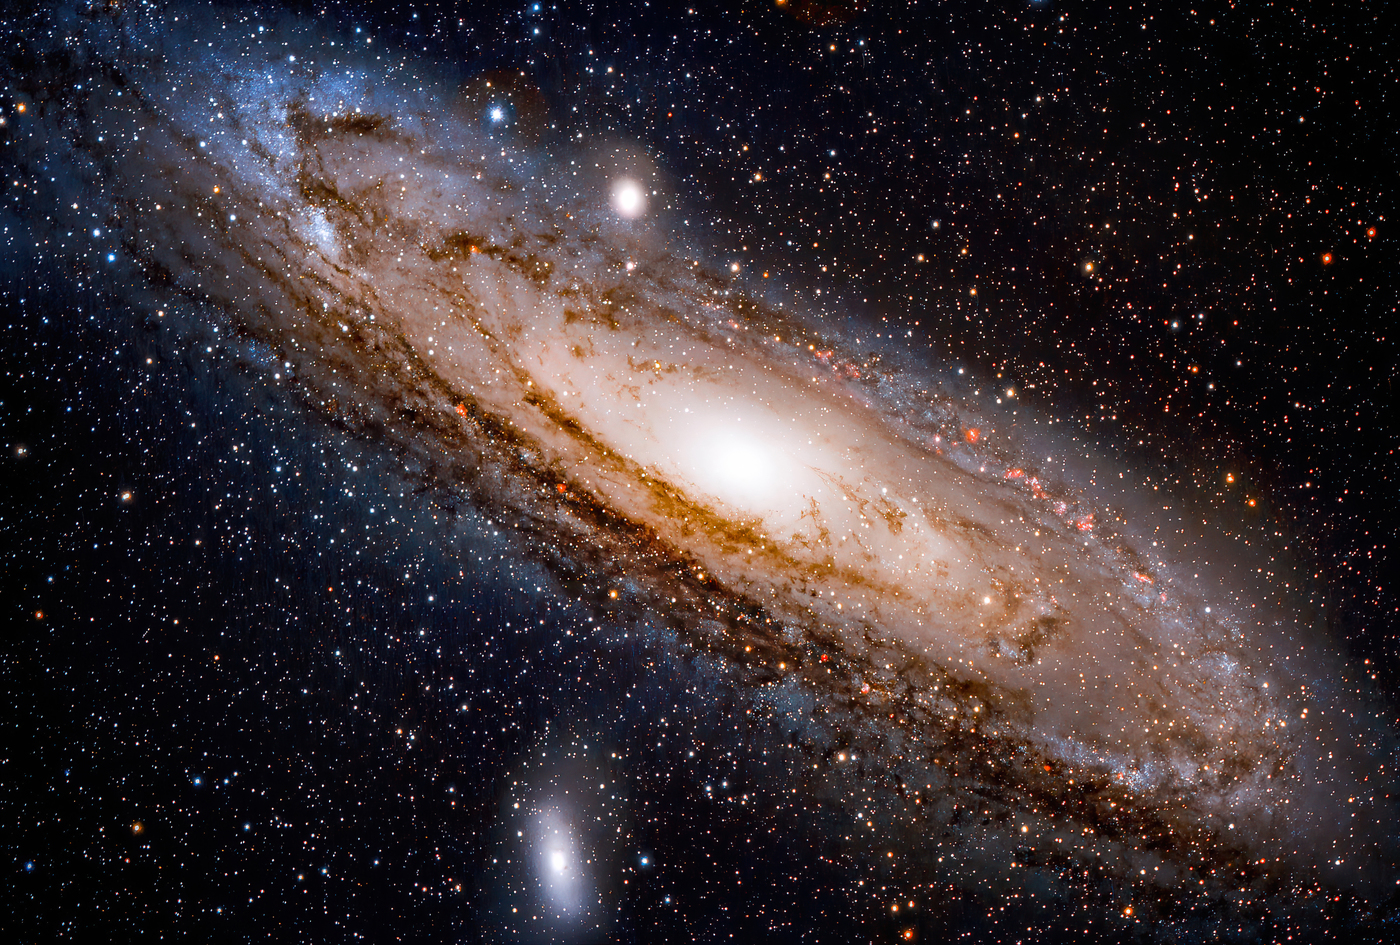
\includegraphics[width=0.99\columnwidth]{images/M31.jpg}\caption{Галактика Туманность Андромеды (М31)}\end{figure}}
\vs p012 2:3 В недалёком будущем\fnst{Написано в 30\hyp{}ых годах XX века.} новые телескопы откроют удивлённому взору астрономов Урантии не менее 375\,000\,000 новых галактик в отдалённых областях внешнего пространства. В то же время эти более мощные телескопы покажут, что многие островные вселенные\fnst{Так раньше назывались галактики (англ. island universes).}, ранее считавшиеся находящимися во внешнем пространстве, на самом деле являются частью галактической системы Орвонтон. Семь сверхвселенных всё ещё растут; периферия каждой из них постепенно расширяется; новые туманности постоянно стабилизируются и организуются; и некоторые из туманностей, которые астрономы Урантии считают внегалактическими, на самом деле находятся на окраине Орвонтона и путешествуют вместе с нами\fnst{Возможно, что речь идёт о Большом и Малом Магеллановых Облаках.}.
\vs p012 2:4 \pc Астрономы [star students] Уверсы отмечают, что большая вселенная окружена предшественниками ряда звёздных и планетарных скоплений, которые полностью окружают нынешнее обитаемое творение в виде концентрических колец внешних многочисленных вселенных. Физики Уверсы подсчитали, что энергия и материя этих внешних и неизведанных областей уже во много раз превышают общую материальную массу и энергетический заряд, заключённый во всех семи сверхвселенных. Мы знаем, что превращение космической силы в этих внешних пространственных уровнях является функцией Райских организаторов силы. Мы также знаем, что эти силы предшествуют тем физическим энергиям, которые в настоящее время активируют большую вселенную. Однако управляющие энергией Орвонтона не имеют никакого отношения к этим удалённым мирам, а движения энергии в них не связаны явным образом с контурами мощи организованных и обитаемых творений.\tunemarkup{pictures}{\begin{figure}[H]\centering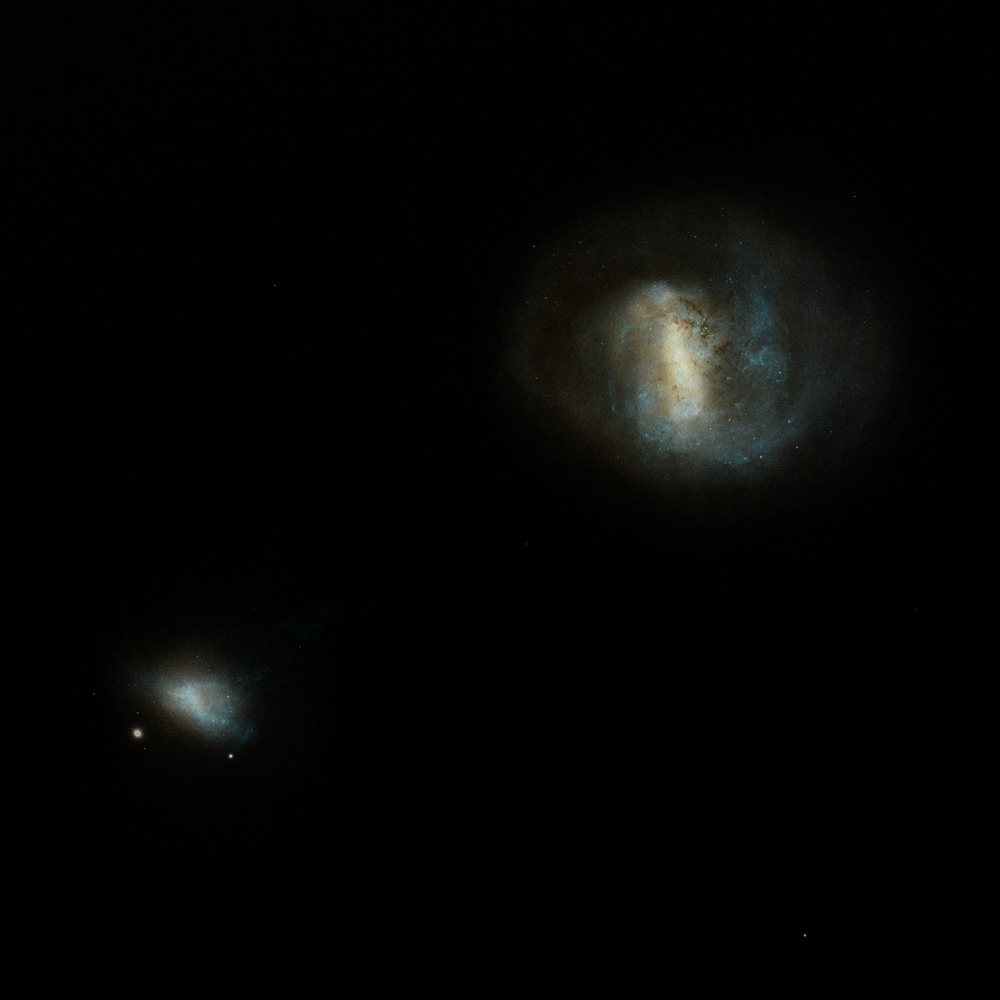
\includegraphics[width=0.99\columnwidth]{images/LMC.jpg}\caption{Большое и Малое Магеллановы Облака}\end{figure}}
\vs p012 2:5 \pc Мы очень мало знаем о значении этих грандиозных явлений внешнего пространства. Ещё более великое творение будущего находится в процессе формирования. Мы наблюдаем его необъятность, мы можем различать его протяжённость и ощущать его величественные размеры, но в остальном мы знаем об этих сферах немногим больше, чем астрономы Урантии. Насколько нам известно, в этом внешнем кольце туманностей, солнц и планет нет материальных существ вроде людей, ангелов или других духовных созданий. Эта далёкая область находится вне юрисдикции и управления правительств сверхвселенных.
\vs p012 2:6 По всему Орвонтону бытует мнение, что имеет место процесс творения нового типа вселенных, которым суждено стать ареной будущих действий собирающегося Корпуса Завершения; и если наши предположения верны, то бесконечное будущее может принести всем вам те же захватывающие дух зрелища, которые бесконечное прошлое содержало для ваших старших поколений [seniors] и предшественников.
\usection{ВСЕОБЩАЯ ГРАВИТАЦИЯ}
\vs p012 3:1 Все формы силы\hyp{}энергии --- материальной, ментальной или духовной --- одинаково подвержены тому охвату, тем универсальным присутствиям, которые мы называем гравитацией. Личность также восприимчива к гравитации --- исключительному контуру Отца; но, хотя этот контур специфически относится именно к Отцу, он\fnst{Отец, а не контур.} не исключён из других контуров; Всеобщий Отец бесконечен и действует по \bibemph{всем} четырём контурам абсолютной гравитации в главной вселенной:
\vs p012 3:2 \li{1.}Гравитация личности Всеобщего Отца.
\vs p012 3:3 \li{2.}Гравитация духа Вечного Сына.
\vs p012 3:4 \li{3.}Гравитация разума Совместного Вершителя.
\vs p012 3:5 \li{4.}Космическая гравитация Острова Рай.
\vs p012 3:6 \pc Эти четыре контура не имеют отношения к силовому центру нижнего Рая; они не являются ни силовыми, ни энергетическими, ни мощностными контурами. Они представляют собой контуры абсолютного \bibemph{присутствия} и, подобно Богу, не зависят от времени и пространства.
\vs p012 3:7 В этой связи интересно упомянуть результаты некоторых наблюдений, сделанных на Уверсе в течение последних тысячелетий корпусом исследователей гравитации. Эта группа экспертов пришла к следующим выводам относительно различных гравитационных систем главной вселенной:
\vs p012 3:8 \li{1.}\bibemph{Физическая гравитация}. Оценив результат суммирования полного потенциала физической гравитации большой вселенной, они тщательно сравнили его с оценкой полной величины ныне действующего присутствия абсолютной гравитации. Эти расчёты показывают, что общее гравитационное воздействие на большую вселенную составляет очень малую часть предполагаемого гравитационного притяжения Рая, вычисленного на основе реакции элементарных физических единиц вселенской материи на гравитацию. Эти исследователи приходят к удивительному выводу, что центральная вселенная и окружающие её семь сверхвселенных в настоящее время используют только около 5\% активно функционирующего охвата абсолютной гравитации Рая. Иными словами: в настоящий момент около 95\% активного действия космической гравитации Острова Рай, вычисленного по этой теории тотальности, задействовано в управлении материальными системами за пределами существующих сегодня организованных вселенных. Все эти расчёты относятся к абсолютной гравитации; линейная гравитация --- это явление взаимодействия, и её можно вычислить, только зная фактическую величину гравитации Рая.
\vs p012 3:9 \li{2.}\bibemph{Духовная гравитация}. Тем же самым методом сравнительной оценки и расчёта эти исследователи изучили текущую способность отклика гравитации духа и, в сотрудничестве с Одиночными Посланниками и другими духовными личностями, получили суммарную величину активной гравитации духа Второго Источника и Центра. И, что особенно поучительно, они обнаружили примерно такое же значение для фактического и функционального присутствия гравитации духа в большой вселенной, какое постулируется ими для полной суммы активной гравитации духа в настоящее время. Иными словами: в настоящее время практически вся гравитация духа Вечного Сына, вычисленная по этой теории тотальности, наблюдается функционирующей в большой вселенной. Если эти открытия достоверны, мы можем заключить, что вселенные, которые сейчас развиваются во внешнем пространстве, в настоящее время полностью недуховны. И если это так, это удовлетворительно объясняет, почему наделённые духом существа почти ничего не знают об этих громадных проявлениях энергии, кроме самог\'о факта их физического существования.
\vs p012 3:10 \li{3.}\bibemph{Гравитация разума}. Используя те же принципы сравнительных вычислений, эти специалисты приступили к решению задачи о присутствии гравитации разума и реакции на неё. Единица разума, принятая для оценки, была получена усреднением трёх материальных и трёх духовных типов мышления, хотя тип разума, присутствующий в управляющих мощью и их партнёрах, оказался мешающим фактором при определении базовой единицы для оценки гравитации разума. В соответствии с данной теорией тотальности оказалось несложным оценить нынешнюю способность Третьего Источника и Центра для функции гравитации разума. Хотя результаты в данном случае не столь убедительны, как в оценках физической и духовной гравитации, при сравнительном рассмотрении они весьма поучительны и даже загадочны. Эти исследователи пришли к выводу, что около 85\% реакции гравитации разума на интеллектуальное притяжение Совместного Вершителя берёт начало в существующей большой вселенной. Это указывает на возможность того, что наблюдаемые физические процессы, ныне происходящие по всем областям внешнего пространства, связаны с активностью разума\fnst{А именно: с остальными 15\% от общей активности разума.}. Хотя эта оценка, вероятно, далеко не точна, она в принципе согласуется с нашими представлениями о том, что разумные организаторы сил в настоящее время направляют эволюцию вселенной на пространственных уровнях за пределами нынешних внешних границ большой вселенной. Какой бы ни была природа этого постулируемого разума, очевидно, что он не реагирует на гравитацию духа.
\vs p012 3:11 Но все эти вычисления в лучшем случае являются оценками, основанными на предполагаемых законах. Мы думаем, что они достаточно надёжны. Даже если несколько духовных существ находятся во внешнем пространстве, их коллективное присутствие не может заметным образом повлиять на вычисления, касающиеся таких масштабных измерений.
\vs p012 3:12 \pc \bibemph{Гравитация личности} невычислима. Мы распознаём этот контур, но не можем измерить ни качественные, ни количественные реальности, реагирующие на него.
\usection{ПРОСТРАНСТВО И ДВИЖЕНИЕ}
\vs p012 4:1 Все единицы космической энергии находятся в первичном вращении, заняты выполнением своей миссии, обращаясь по вселенской орбите. Вселенные пространства и их составные системы и миры представляют собой вращающиеся сферы, движущиеся по бесконечным контурам уровней пространства главной вселенной. Во всей главной вселенной нет абсолютно ничего неподвижного, кроме с\'амого центра Хавоны, вечного Острова Рай, центра гравитации.
\vs p012 4:2 Безусловный Абсолют функционально ограничен пространством, но мы не столь уверены относительно связи этого Абсолюта с движением. Присуще ли ему движение? Мы не знаем. Мы знаем, что движение не присуще пространству; даже движения \bibemph{самог\'о} пространства не являются врождёнными. Но мы не столь уверены относительно связи Безусловного с движением. Кто или что на самом деле отвечает за гигантские процессы трансмутации силы\hyp{}энергии, которые сейчас продолжаются за пределами нынешних семи сверхвселенных? Относительно происхождения движения у нас есть следующие мнения:
\vs p012 4:3 \li{1.}Мы думаем, что Совместный Вершитель инициирует движение \bibemph{в} пространстве.
\vs p012 4:4 \li{2.}Если Совместный Вершитель и производит движения \bibemph{самог\'о} пространства, мы не можем этого доказать.
\vs p012 4:5 \li{3.}Всеобщий Абсолют не порождает первоначальное движение, но он стабилизирует и контролирует все напряжения, порождаемые движением.
\vs p012 4:6 \pc Во внешнем пространстве организаторы сил, по\hyp{}видимому, отвечают за создание гигантских вселенских дисков, которые сейчас находятся в процессе звёздообразования, но их способность функционировать таким образом, должно быть, стала возможной благодаря некоторой модификации космического присутствия Безусловного Абсолюта.\tunemarkup{pictures}{\begin{figure}[H]\centering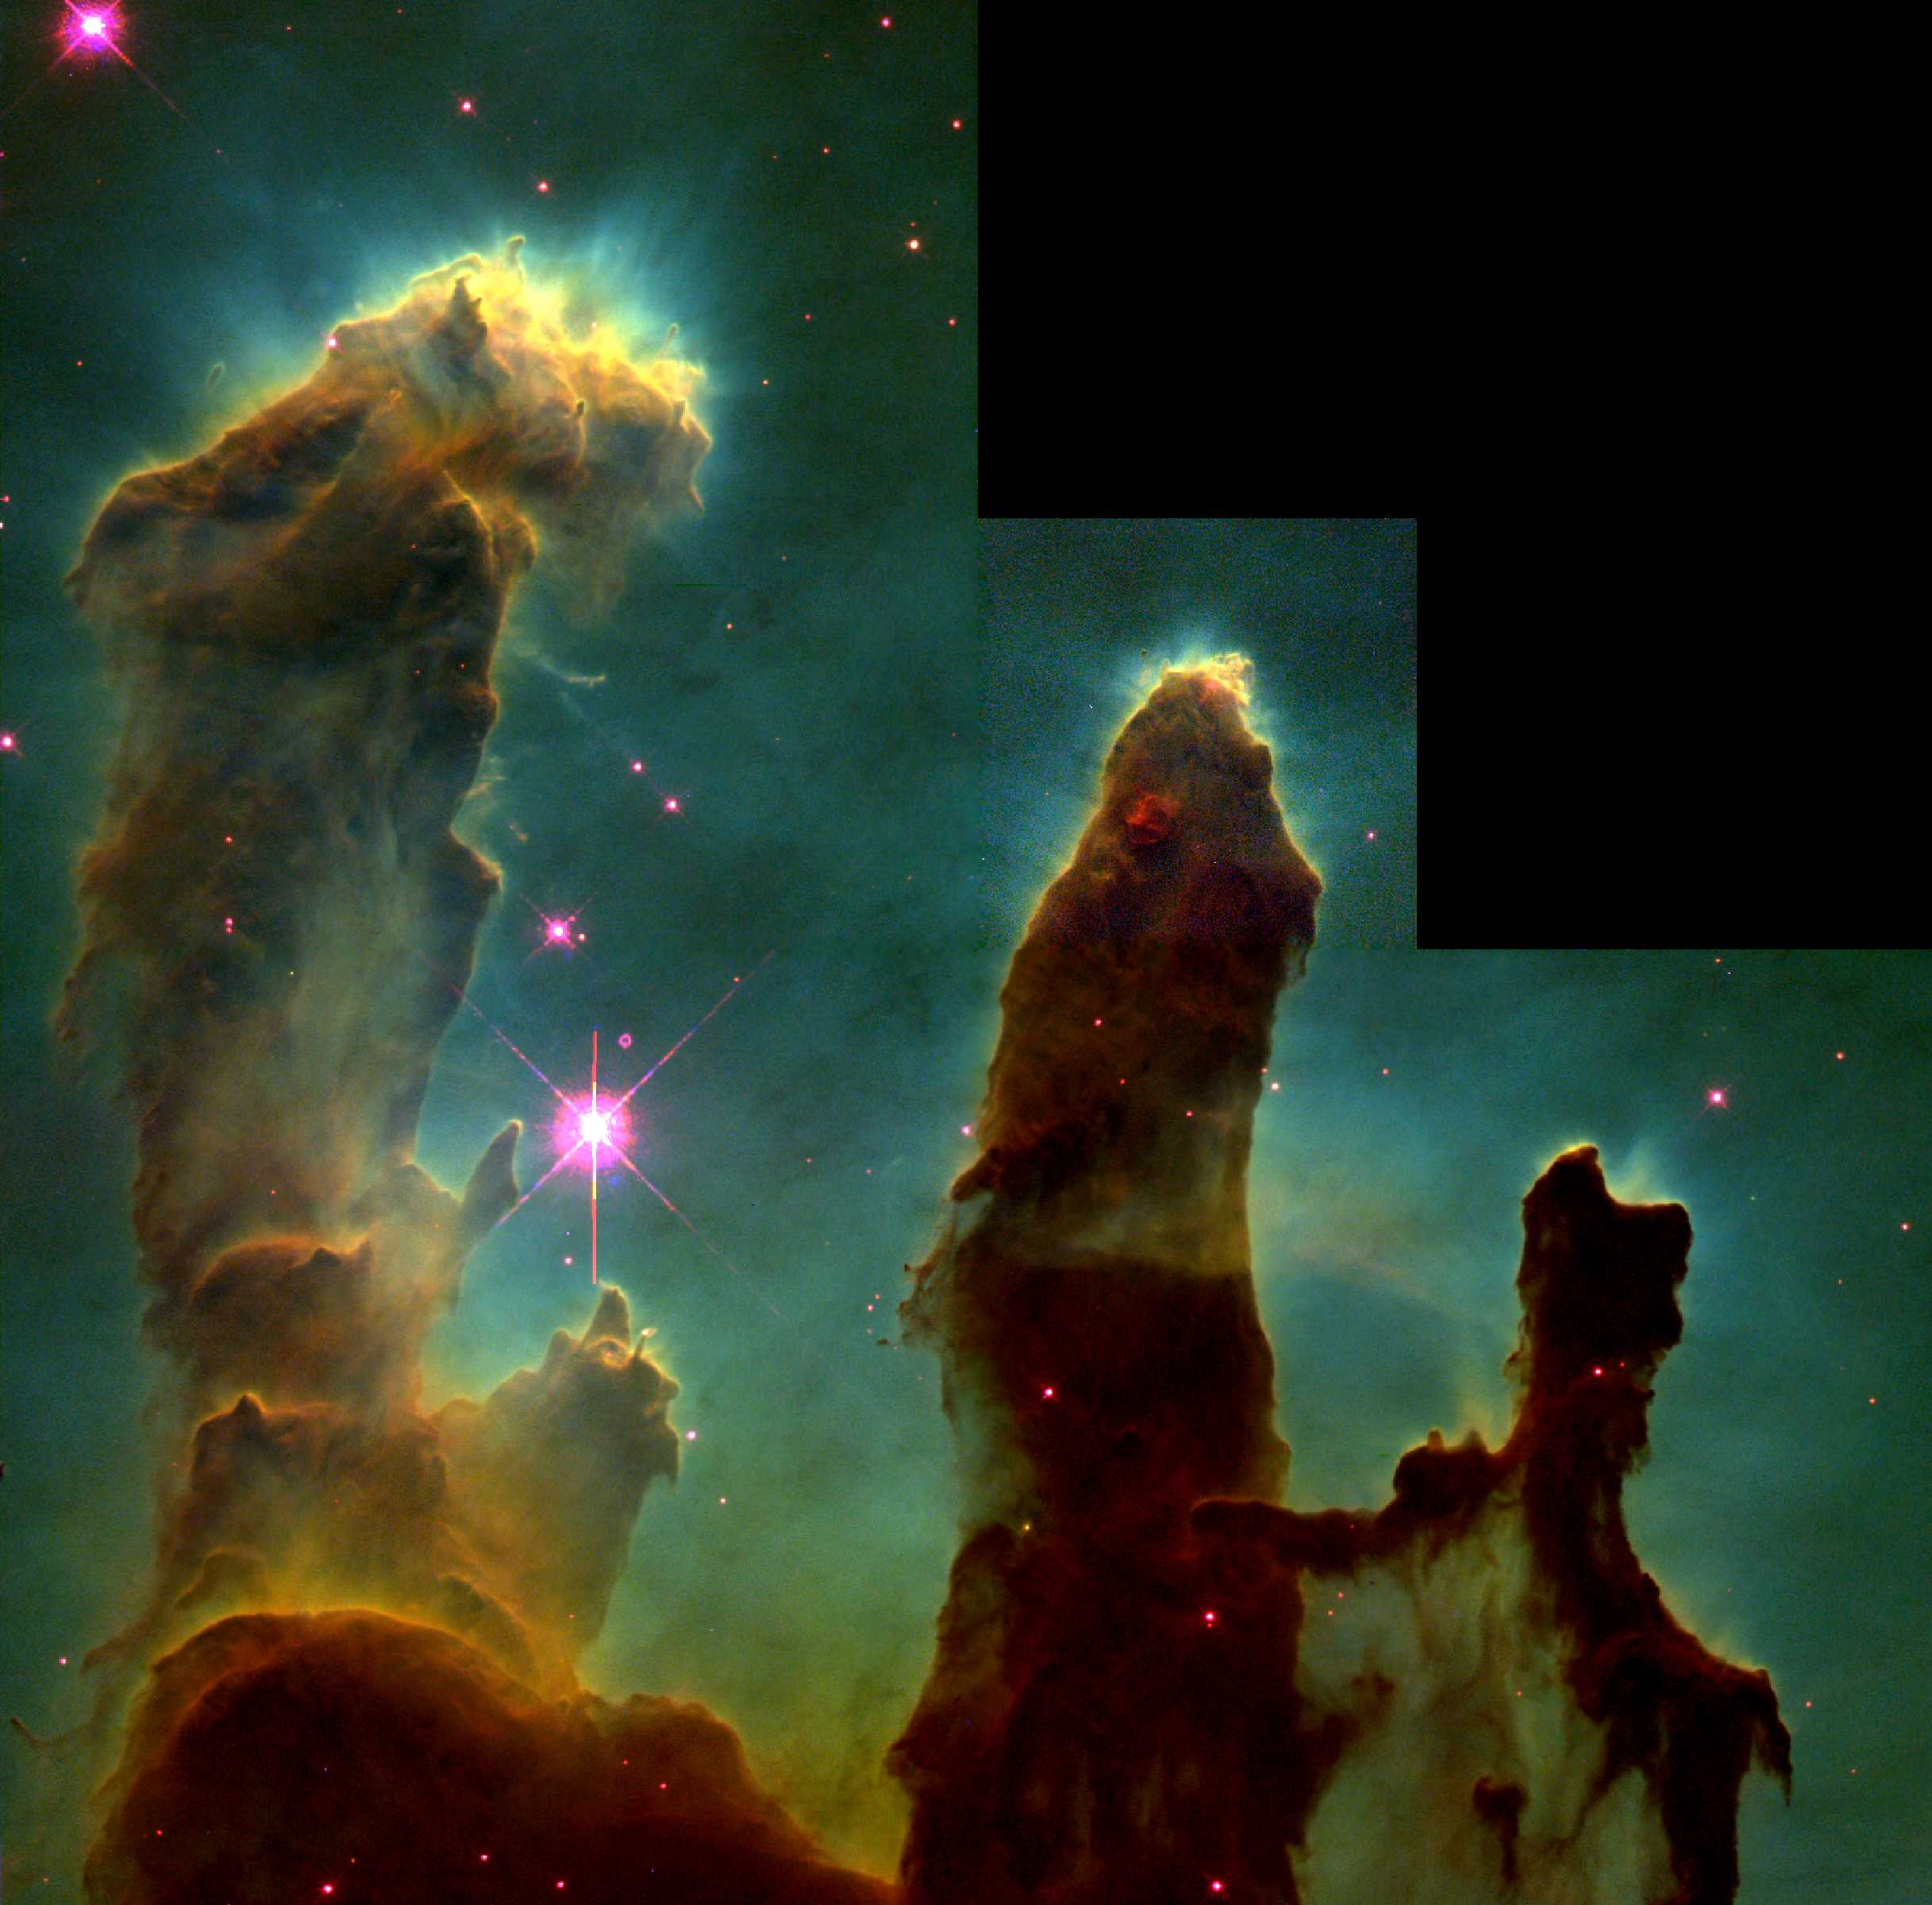
\includegraphics[width=0.99\columnwidth]{images/Stolpy-tvoreniya.jpg}\caption{<<Столпы творения>> в туманности Орёл}\end{figure}}
\vs p012 4:7 \pc Пространство, с человеческой точки зрения, --- это ничто, нечто отрицательное; оно существует только по отношению к чему\hyp{}то положительному и непространственному. Тем не менее пространство реально. Оно содержит и обуславливает движение. Оно даже движется. Движения пространства можно приблизительно классифицировать следующим образом:
\vs p012 4:8 \li{1.}Первичное движение --- респирация\fnst{Дыхание.} пространства, движение самог\'о пространства.
\vs p012 4:9 \li{2.}Вторичное движение --- противоположно направленные обращения последовательных уровней пространства.
\vs p012 4:10 \li{3.}Относительные движения --- относительные в том смысле, что они не вычисляются относительно Рая как точки отсчёта. Первичные и вторичные движения абсолютны, это движения относительно неподвижного Рая.
\vs p012 4:11 \li{4.}Компенсирующее или коррелирующее перемещение, предназначенное для координации всех остальных типов движения.
\vs p012 4:12 \pc Нынешнее взаимоотношение вашего Солнца и связанных с ним планет хотя и раскрывает множество относительных и абсолютных движений в пространстве, но создаёт впечатление у астрономов\hyp{}наблюдателей, что вы сравнительно неподвижны в пространстве, а ваши вычисления, охватывающие всё новые глубины пространства, указывают на то, что окружающие звёздные скопления и потоки вовлечены в направленный вовне полёт с постоянно возрастающими скоростями. Но это не так. Вы не принимаете во внимание нынешнее однородное расширение физических творений всего насыщенного пространства. Ваше собственное локальное творение (Небадон) участвует в этом движении всеобщего расширения. Все семь сверхвселенных участвуют в цикле пространственной респирации, длительностью в два миллиарда лет, вместе с внешними областями главной вселенной.
\vs p012 4:13 Когда вселенные расширяются и сжимаются, материальные массы в насыщенном пространстве попеременно движутся против и по направлению притяжения Райской гравитации. Работа, совершаемая при перемещении материальной энергетической массы творения, есть работа \bibemph{пространственная,} а не работа \bibemph{мощи\hyp{}энергии}.
\vs p012 4:14 \pc Хотя ваши спектроскопические оценки астрономических скоростей достаточно надёжны в применении к звёздным мирам, принадлежащим вашей и соседним сверхвселенным, такие расчёты совершенно непригодны к мирам внешнего пространства. Спектральные линии приближающейся звезды смещены в фиолетовую сторону; и, наоборот, у удаляющейся звезды эти линии смещаются в красную сторону. Многие факторы, накладываясь, создают впечатление, будто скорость удаления внешних вселенных увеличивается с расстоянием более чем на 160~км/с на каждый 1\,000\,000 световых лет\fnst{Приведённое в тексте Откровения значение постоянной Хаббла (522\,км/c/Мпк) близко к полученному самим Хабблом в 1935\,г. значению 535\,км/с/Мпк. Вычисления Хаббла были основаны на зависимости между периодом и светимостью переменных звёзд, именуемых цефеидами. Пересмотр нуль\hyp{}пункта этой зависимости (В.\,Бааде, 1952\,г.) привёл к коррекции величины постоянной Хаббла. К 1955\,г. общепринятым значением являлось 180\,км/с/Мпк. Современное (2016\,г.) значение и того меньше: 66,93$\pm$0,62\,км/с/Мпк.}. С усовершенствованием более мощных телескопов подобные рассуждения приведут к выводу, что эти далёкие системы удаляются из данной части вселенной с невероятной скоростью, превышающей 48\,000~км/с. Но эта кажущаяся скорость удаления нереальна; она является результатом множества факторов, приводящих к ошибке, включая углы наблюдения и другие время\hyp{}пространственные искажения.
\vs p012 4:15 Но наибольшее искажение возникает из\hyp{}за того, что огромные вселенные внешнего пространства в сферах, следующих за областями семи сверхвселенных, по\hyp{}видимому, вращаются в направлении, противоположном направлению вращения большой вселенной. То есть эти мириады туманностей и сопровождающих их солнц и сфер в настоящее время вращаются по часовой стрелке вокруг центрального творения. Семь сверхвселенных вращаются вокруг Рая против часовой стрелки. Представляется, что вторая внешняя вселенная галактик, как и семь сверхвселенных, вращается против часовой стрелки вокруг Рая. И астрономы\hyp{}наблюдатели Уверсы полагают, что они обнаружили доказательства вращательных движений в третьем внешнем поясе далёкого пространства, которые начинают проявлять тенденции направленности по часовой стрелке.
\vs p012 4:16 Вероятно, что эти попеременные направления последовательных процессий вселенных в пространстве имеют какое\hyp{}то отношение к механизму гравитации Всеобщего Абсолюта, действующему внутри главной вселенной и заключающемуся в координации сил и выравнивании пространственных напряжений. Движение так же, как и пространство, дополняет или уравновешивает гравитацию.
\usection{ПРОСТРАНСТВО И ВРЕМЯ}
\vs p012 5:1 Как и пространство, время есть дар Рая, но не в том же смысле, а лишь косвенно. Время возникает благодаря движению и потому, что разум изначально осознаёт последовательность. С практической точки зрения движение является существенным для времени, однако не существует универсальной единицы времени, основанной на движении, за исключением стандартного дня Рая\hyp{}Хавоны, произвольно принятого за таковую. Тотальность респирации пространства разрушает его локальную ценность в качестве источника времени.
\vs p012 5:2 Пространство не бесконечно, хотя оно и берёт начало из Рая; не абсолютно, ибо оно пронизано Безусловным Абсолютом. Мы не знаем абсолютных пределов пространства, но мы знаем, что абсолютом времени является вечность.
\vs p012 5:3 \pc Время и пространство неразделимы только во время\hyp{}пространственных творениях --- семи сверхвселенных. Нетемпоральное пространство (пространство без времени) теоретически существует, но единственным действительно нетемпоральным местом является \bibemph{площадь}\fnst{Именно \bibemph{площадь} (англ. \bibemph{area}). Связано ли это как\hyp{}то со свойством фазового пространства, в котором не существует расстояния между двумя точками $(x_1,p_1)$ и $(x_2,p_2)$, но вполне можно говорить о \bibemph{площади} треугольника с вершинами в трёх точках $(x_1,p_1)$, $(x_2,p_2)$ и $(x_3,p_3)$? Именно эта площадь странным образом фигурирует в эволюционных пропагаторах квантовой механики, переформулированной в терминах функций Вигнера.} Рая. Непространственное время (время без пространства) существует в разуме, функционирующем на уровне Рая.
\vs p012 5:4 Относительно неподвижные зоны промежуточного пространства, примыкающие к Раю и отделяющие насыщенное пространство от ненасыщенного, являются зонами перехода от времени к вечности, поэтому Райские пилигримы должны терять сознание во время этого перехода, когда он должен увенчаться Райским гражданством. Сознающие время \bibemph{посетители} могут попасть в Рай, не впадая в такой сон, но они остаются созданиями времени.
\vs p012 5:5 \pc Временн\'ые связи не существуют без движения в пространстве, но осознание времени существует. Понятие последовательности\fnst{Видимо, <<последовательности событий>>.} позволяет осознавать время даже в отсутствие движения. По своей природе человеческий разум меньше привязан ко времени, чем к пространству. Даже во дни земной жизни во плоти человеческий разум жёстко привязан к пространству, в то время как творческое воображение человека относительно свободно от времени. Но само время не является генетическим качеством разума.
\vs p012 5:6 \pc Существует три разных уровня восприятия времени\fnst{В то время как существует \bibemph{семь} различных концепций пространства, обусловленного временем. См.\,\bibref[130:7.6]{p130 7:6}.}:
\vs p012 5:7 \li{1.}Время, воспринимаемое разумом, --- осознание последовательности, движения и ощущение продолжительности.
\vs p012 5:8 \li{2.}Время, воспринимаемое духом, --- проникновение в суть движения по направлению к Богу и осознание восходящего движения по уровням возрастающей божественности.
\vs p012 5:9 \li{3.}Личность \bibemph{создаёт} уникальное чувство времени из проникновения в суть Реальности плюс сознания присутствия и осознания продолжительности.
\vs p012 5:10 \pc Бездуховные животные знают только прошлое и живут настоящим. Человек, в котором пребывает дух, обладает способностью предвидения (проницательности); он может представить себе будущее. Только обращённые в будущее и прогрессивные взгляды являются реальными для личности. Статическая этика и традиционная мораль лишь немного сверхживотны. Не является высоким видом самореализации и стоицизм. Этика и мораль становятся истинно человеческими тогда, когда они динамичны и прогрессивны, наполнены жизнью вселенской реальности.
\vs p012 5:11 Человеческая личность не просто сопутствует время\hyp{}пространственным событиям; человеческая личность может также действовать в качестве космической причины таких событий.
\usection{ВСЕОБЩЕЕ СВЕРХУПРАВЛЕНИЕ}
\vs p012 6:1 Вселенная не статична. Стабильность --- не результат инерции, но, скорее, результат сбалансированных энергий, сотрудничающих разумов, скоординированных моронтий, сверхконтроля духа и объединения личности. Стабильность целиком и всегда пропорциональна божественности.
\vs p012 6:2 В физическом управлении главной вселенной Всеобщий Отец осуществляет приоритет и первенство через Остров Рай; Бог абсолютен в духовном управлении космосом в лице Вечного Сына. Что касается областей разума, Отец и Сын согласованно действуют в Совместном Вершителе.
\vs p012 6:3 Третий Источник и Центр помогает в поддержании равновесия и координации объединённых физических и духовных энергий и формирований посредством абсолютности своего охвата космического разума и благодаря проявлению присущих ему и универсальных дополнений физической и духовной гравитации. Когда бы и где бы ни возникала связь между материальным и духовным, такое явление разума является действием Бесконечного Духа. Только разум может осуществлять взаимосвязь физических сил и энергий материального уровня с духовными силами и существами уровня духа.
\vs p012 6:4 Во всех твоих размышлениях о вселенских явлениях убедись, что ты принимаешь во внимание взаимосвязь физических, интеллектуальных и духовных энергий и что должным образом учитываешь неожиданные явления, сопровождающие их объединение личностью, и непредсказуемые явления, возникающие в результате действия и реакции эмпирического Божества и Абсолютов.
\vs p012 6:5 Вселенная в высшей степени предсказуема только в количественном смысле, --- в смысле измерения гравитации; даже первичные физические силы не реагируют на линейную гравитацию, равно как и смыслы высшего разума и истинные духовные ценности предельных вселенских реальностей. В качественном смысле Вселенная не очень предсказуема в отношении новых ассоциаций сил --- физических, ментальных или духовных, --- хотя многие такие комбинации энергий или сил становятся частично предсказуемыми, когда подвергаются критическому наблюдению. Когда материя, разум и дух объединены личностью создания, мы не можем полностью предсказать решения такого существа, обладающего свободной волей.
\vs p012 6:6 \pc Все фазы изначальной силы, зарождающегося духа и других неличностных предельностей, по\hyp{}видимому, реагируют в соответствии с некоторыми относительно стабильными, но неизвестными законами и характеризуются широтой действия и гибкостью реакции, которые часто приводят в замешательство, когда встречаются в явлениях ограниченных и изолированных ситуаций. Каково объяснение этой непредсказуемой свободы реакции, обнаруживаемой этими возникающими вселенскими актуальностями? Эти неизвестные, непостижимые непредсказуемости, --- относятся ли они к поведению первичной единицы силы, реакции неопознанного уровня разума или феномену обширной предвселенной, создаваемой в областях внешнего пространства, --- вероятно, раскрывают деятельность Предельного и присутствие\hyp{}действие Абсолютов, предшествующих функционированию всех вселенских Создателей.
\vs p012 6:7 Хотя доподлинно нам это неизвестно, мы предполагаем, что такая удивительная разносторонность и такая глубокая координация означают присутствие и действие Абсолютов, и что такое разнообразие реакций при явно однородной причинности раскрывает реакцию Абсолютов, --- и не только на непосредственную и ситуативную причину, но также и на все другие родственные причины по всей главной вселенной.
\vs p012 6:8 \pc У индивидуумов есть свои хранители предназначения; планеты, системы, созвездия, вселенные и сверхвселенные --- все имеют своих соответствующих правителей, которые трудятся на благо своих владений. За Хавоной, и даже большой вселенной, наблюдают те, кому доверена столь высокая ответственность. Но кто взращивает и заботится о фундаментальных потребностях главной вселенной в целом --- от Рая до четвёртого и самого дальнего пространственного уровня? Экзистенциально такую сверхзаботу, вероятно, можно приписывать Райской Троице, но с эмпирической точки зрения появление вселенных после Хавоны зависит от:
\vs p012 6:9 \li{1.}Абсолютов --- в потенциале.
\vs p012 6:10 \li{2.}Предельного --- в направлении.
\vs p012 6:11 \li{3.}Верховного --- в эволюционной координации.
\vs p012 6:12 \li{4.}Архитекторов Главной Вселенной --- в управлении до появления специальных правителей.
\vs p012 6:13 \pc Безусловный Абсолют пронизывает всё пространство. Нам не вполне ясен точный статус Божественного и Всеобщего Абсолютов, но мы знаем, что последний действует везде, где действуют Божественный и Безусловный Абсолюты. Божественный Абсолют может присутствовать повсюду, но вряд ли возможно его пространственное присутствие. Предельный присутствует или когда\hyp{}нибудь будет присутствовать в пространстве до внешних границ четвёртого пространственного уровня. Мы сомневаемся, что Предельный будет когда\hyp{}либо иметь пространственное присутствие за периферией главной вселенной, но в этих границах Предельный постепенно объединяет творческую структуру потенциалов трёх Абсолютов.
\usection{ЧАСТЬ И ЦЕЛОЕ}
\vs p012 7:1 Во всём времени и пространстве и по отношению ко всей реальности любой природы действует неумолимый и беспристрастный закон, эквивалентный функции космического провидения. Милосердие характеризует отношение любви Бога к индивидууму; беспристрастность мотивирует отношение Бога к целому. Воля Бога не обязательно преобладает в части --- в сердце любой отдельно взятой личности, --- но его воля действительно управляет целым --- вселенной вселенных.
\vs p012 7:2 \pc Истинно, что во всех его отношениях со всеми своими существами законы Бога не являются по своей сути произвольными. Тебе, с твоим ограниченным в\'идением и конечной точкой зрения, деяния Бога часто должны казаться диктаторскими и произвольными. Законы Бога --- это просто привычки Бога, его способ делать что\hyp{}то повторяющееся; и он всегда всё делает хорошо. Ты можешь заметить, что Бог делает одно и то же тем же самым образом просто потому, что это лучший способ сделать эту конкретную вещь в данных обстоятельствах; а лучший способ и есть правильный, и поэтому бесконечная мудрость всегда предписывает, чтобы это было сделано именно таким точным и совершенным образом. Тебе следует также помнить, что природа не является исключительным действием Божества; другие влияния присутствуют в тех явлениях, которые человек называет природой.
\vs p012 7:3 Божественной природе невыносимо терпеть любую форму деградации или даже разрешать совершение какого\hyp{}либо чисто личного действия не самым лучшим образом. Однако следует прояснить, что \bibemph{если} в божественности любой ситуации, в экстремальности любых обстоятельств, в любом случае, когда следование верховной мудрости может указать требование иного поведения, --- если требования совершенства по какой\hyp{}либо причине диктуют другой, лучший способ реагирования, --- тогда премудрый Бог сразу же поступит таким лучшим и более подходящим способом. И это будет выражением высшего закона, а не отменой низшего.
\vs p012 7:4 Бог не является рабом привычки хронического повторения своих собственных добровольных действий. Между законами Бесконечного нет противоречий; все они --- совершенства непогрешимой природы; все они --- неоспоримые действия, выражающие безупречные решения. Закон --- это неизменная реакция бесконечного, совершенного и божественного разума. Все деяния Бога являются волевыми, несмотря на их кажущуюся одинаковость. В Боге <<нет ни изменчивости, ни тени перемены>>\fnst{Цитата из Иакова~1:17.}. Но всё то, что может воистину быть сказано о Всеобщем Отце, не может быть с такой же уверенностью сказано обо всех подчинённых ему разумных существах или о его эволюционных созданиях.
\vs p012 7:5 Поскольку Бог неизменен, ты можешь во всех обычных обстоятельствах положиться на то, что он делает то же самое таким же идентичным и обычным образом. Бог --- гарантия стабильности для всех созданных вещей и существ. Он Бог; поэтому он не меняется.
\vs p012 7:6 И всё это постоянство поведения и единообразие действий являются личными, сознательными и в высшей степени волевыми, ибо великий Бог не является беспомощным рабом своего собственного совершенства и бесконечности. Бог --- это не самодействующая автоматическая сила; он не рабская законопослушная власть. Бог --- это ни математическое уравнение, ни химическая формула. Он --- первичная личность, обладающая свободой воли. Он является Всеобщим Отцом, существом, преисполненным личностью, и универсальным источником личности всех созданий.
\vs p012 7:7 \pc Воля Бога не постоянно побеждает в сердце ищущего Бога материального смертного, но если временн\'ые рамки расширить за пределы данного момента, охватывая всю первую жизнь, тогда воля Бога становится всё более заметной в духовных плодах, принесённых в жизнях ведомых духом детей Божьих. А затем, если человеческую жизнь ещё больше расширить, включив моронтийный опыт, то можно заметить, как божественная воля сияет всё ярче и ярче в одухотворяющих поступках тех созданий времени, которые начали ощущать вкус божественных наслаждений эмпирического переживания связи личности человека с личностью Всеобщего Отца.
\vs p012 7:8 Отцовство Бога и братство людей представляют собой парадокс части и целого на уровне личности. Бог любит \bibemph{каждого} индивидуума как отдельное дитя в небесной семье. В то же время Бог любит так же \bibemph{всех} индивидуумов; он нелицеприятен, и универсальность его любви порождает отношение целого --- всеобщее братство.
\vs p012 7:9 Любовь Отца абсолютно индивидуализирует каждую личность как уникальное дитя Всеобщего Отца, --- дитя без дубликатов в бесконечности, волевое создание, незаменимое во всей вечности. Любовь Отца возносит каждое дитя Бога, озаряя каждого члена небесной семьи, резко выделяя уникальную природу каждого личностного существа на фоне неличностных уровней, лежащих за пределами братского контура Отца всех. Любовь Бога поразительно отображает трансцендентную ценность каждого волевого создания, безошибочно раскрывает высокую ценность, которую Всеобщий Отец придаёт каждому из своих детей и всем им, --- от высшей личности создателя с Райским статусом до низшей личности волевого достоинства среди диких племён на заре человеческого рода в каком\hyp{}нибудь эволюционном мире времени и пространства.
\vs p012 7:10 Именно эта любовь Бога к индивидууму порождает божественную семью всех индивидуумов, всеобщее братство добровольных детей Райского Отца. И это братство, будучи всеобщим, является отношением целого. Братство, если оно всеобщее, раскрывает не отношение \bibemph{каждого,} а отношение \bibemph{всех}. Братство --- это реальность целого и поэтому раскрывает свойства целого в противоположность свойствам части.
\vs p012 7:11 Братство составляет факт отношения между каждой личностью во вселенском существовании. Ни одно лицо не может избежать преимуществ или потерь, которые могут возникнуть в результате отношений с другими лицами. Благополучие или страдания части соизмеримы с таковыми целого. Попытки каждого человека делать добро приносят пользу всем людям; ошибка или зло каждого человека усугубляет несчастье всех людей. Как движется часть, так движется и целое. Каков прогресс целого, таков прогресс и части. Относительные скорости части и целого определяют, будет ли часть замедляться инертностью целого или переноситься вперёд импульсом космического братства.
\vs p012 7:12 \pc Остаётся тайной, каким образом Бог, будучи высоколичностным, самосознающим существом, имеющим постоянную резиденцию, в то же самое время лично присутствует в такой огромной вселенной и лично находится в контакте практически с бесконечным числом существ. То, что данное явление является тайной за пределами человеческого понимания, не должно ни в коей мере умалять твою веру. Не позволяй громадности бесконечности, необъятности вечности, величию и славе несравненного характера Бога внушать тебе благоговейный страх, ошеломлять или обескураживать тебя; ибо Отец недалеко от любого из вас; он обитает внутри тебя, и в нём мы все буквально движемся, действительно живём и истинно обретаем наше бытие.
\vs p012 7:13 \pc Несмотря на то что Райский Отец действует через своих божественных создателей и своих детей\hyp{}созданий, он также поддерживает с тобой самую сокровенную связь, --- связь столь возвышенную, столь высоко личную, что она выходит за пределы даже моего понимания, --- то таинственное общение фрагмента Отца с человеческой душой и смертным разумом своего действительного пребывания. Исходя из того, что тебе уже известно об этих дарах Бога, ты должен понимать, что Отец находится в тесном контакте не только со своими божественными партнёрами, но и со своими эволюционными смертными детьми времени. Отец действительно обитает на Рае, но его божественное присутствие также обитает в разумах людей.
\vs p012 7:14 Хотя дух Сына и был излит на всю плоть, хотя Сын и жил когда\hyp{}то с вами в подобии смертной плоти, хотя серафимы лично охраняют и ведут вас, как может любое из этих божественных существ Второго и Третьего Центров надеяться подойти к вам так же близко или понять вас так же полно, как Отец, который отдал часть себя, чтобы быть в вас, чтобы быть вашим настоящим, божественным и даже вашим вечным <<я>>?
\usection{МАТЕРИЯ, РАЗУМ И ДУХ}
\vs p012 8:1 <<Бог есть дух>>, но Рай --- нет. Материальная вселенная всегда является ареной, на которой происходит вся духовная деятельность; духовные существа и восходящие духи живут и работают на физических сферах материальной реальности.
\vs p012 8:2 \pc Дар космической силы, область космической гравитации --- это функция Острова Рай. Вся изначальная сила\hyp{}энергия исходит из Рая, а материя для создания бессчётных вселенных в настоящее время циркулирует по всей главной вселенной в форме присутствия супергравитации, которое составляет силу\hyp{}заряд насыщенного пространства.
\vs p012 8:3 Какие бы трансформации ни претерпевала сила в далёких вселенных, выйдя из Рая, она продолжает путешествовать, подчиняясь нескончаемому, вездесущему, неизменному притяжению вечного Острова, послушно и присущим ей образом обращаясь по вечным пространственным траекториям вселенных. Физическая энергия --- это единственная реальность, которая является верной и постоянной в своём подчинении всеобщему закону. Только в сферах воли созданий происходит отклонение от божественных путей и изначальных планов. Мощь и энергия --- универсальные свидетельства стабильности, постоянства и вечности центрального Острова Рай.
\vs p012 8:4 \pc Посвящение духа и одухотворение личностей, сфера духовной гравитации --- это сфера Вечного Сына. И эта гравитация духа Сына, постоянно притягивающая к нему все духовные реальности, так же реальна и абсолютна, как всесильный материальный охват Острова Рай. Но человек, склонный к материальному, естественно, более знаком с материальными проявлениями физической природы, чем с такими же реальными и могущественными действиями духовной природы, которые можно различить только духовной проницательностью души.
\vs p012 8:5 По мере того как разум любой личности во вселенной становится более духовным --- Богоподобным, --- он становится менее реагирующим на материальную гравитацию. Реальность, измеряемая реакцией на физическую гравитацию, является противоположностью реальности, определяемой качеством духовного содержания. Действие физической гравитации является количественным показателем недуховной энергии; действие духовной гравитации является качественной мерой живой энергии божественности.
\vs p012 8:6 \pc Чем Рай является для физического творения и Вечный Сын --- для духовной вселенной, тем Совместный Вершитель является для областей разума --- разумной вселенной материальных, моронтийных и духовных существ и личностей.
\vs p012 8:7 Совместный Вершитель реагирует как на материальные, так и на духовные реальности, и поэтому, по своей сущности, становится универсальным служителем для всех разумных существ, --- существ, которые могут представлять собой союз как материальной, так и духовной фаз творения. Наделение разумом, помощь материальному и духовному посредством феномена разума является исключительной прерогативой Совместного Вершителя, который, таким образом, становится партнёром духовного разума, сущностью моронтийного разума и субстанцией материального разума эволюционных созданий времени.
\vs p012 8:8 Разум --- это метод, с помощью которого реальности духа становятся эмпирическими для личностей созданий. И в конечном счёте объединяющие возможности даже человеческого разума, --- способность координировать вещи, идеи и ценности --- являются сверхматериальными.
\vs p012 8:9 \pc Хотя смертному разуму вряд ли возможно постичь семь уровней относительной космической реальности, человеческий интеллект должен понять б\'ольшую часть смысла трёх действующих уровней конечной реальности:
\vs p012 8:10 \li{1.}\bibemph{Материя}. Организованная энергия, которая подчинена линейной гравитации, за исключением того, что она модифицируется движением\fnst{В каком смысле материя \bibemph{модифицируется} движением? Здесь лежит великая загадка.} и обусловливается разумом.
\vs p012 8:11 \li{2.}\bibemph{Разум}. Организованное сознание, которое не полностью подчинено материальной гравитации и которое становится воистину освобождённым, когда оно модифицировано духом.
\vs p012 8:12 \li{3.}\bibemph{Дух}. Высшая личностная реальность. Истинный дух не подчиняется физической гравитации, но в итоге становится мотивирующим влиянием для всех развивающихся энергетических систем уровня достоинства личности.
\vs p012 8:13 \pc Цель существования всех личностей --- дух; материальные проявления относительны, и космический разум служит посредником между этими всеобщими противоположностями. Наделение разумом и служение духа --- это работа связанных личностей Божества --- Бесконечного Духа и Вечного Сына. Тотальная реальность Божества --- это не разум, а дух\hyp{}разум --- разум\hyp{}дух, объединённый личностью. Тем не менее абсолюты как духа, так и вещи сходятся в личности Всеобщего Отца.
\vs p012 8:14 \pc На Рае согласованы три вида энергии: физическая, ментальная и духовная. В эволюционном космосе преобладает энергия\hyp{}материя, за исключением личности, где дух через посредство разума стремится к господству. Дух есть фундаментальная реальность личностного опыта всех созданий, потому что Бог есть дух. Дух неизменен, и поэтому во всех личностных отношениях он превосходит как разум, так и материю, которые являются эмпирическими переменными прогрессивного достижения.
\vs p012 8:15 В космической эволюции материя становится философской тенью, отбрасываемой разумом в присутствии духовного сияния божественного просвещения, но это не отменяет реальности материи\hyp{}энергии. Разум, материя и дух одинаково реальны, но не имеют одинаковой ценности для личности в достижении божественности. Сознание божественности --- это постепенный духовный опыт.
\vs p012 8:16 Чем ярче сияние одухотворённой личности (Отца во вселенной, фрагмента потенциальной духовной личности в индивидуальном создании), тем сильнее тень, отбрасываемая посредником\hyp{}разумом на своё материальное облачение. Во времени тело человека так же реально, как разум или дух, но после смерти разум (индивидуальность) и дух выживают, а тело --- нет. Космическая реальность может быть несуществующей в опыте личности. И поэтому ваша греческая метафора --- материальное как тень более реальной духовной субстанции --- действительно имеет философское значение.
\usection{ЛИЧНОСТНЫЕ РЕАЛЬНОСТИ}
\vs p012 9:1 Дух --- это основная личностная реальность во вселенных, а личность --- это основа всякого постепенного опыта духовной реальности. Каждая фаза личностного опыта на каждом последовательном уровне вселенского развития изобилует подсказками [clues] к открытию заманчивых личностных реальностей. Истинное предназначение человека состоит в создании новых духовных целей и затем в отклике на космический зов этих возвышенных целей нематериальной ценности.
\vs p012 9:2 \pc Любовь --- это секрет благотворного общения между личностями. Невозможно по\hyp{}настоящему узнать человека на основании единичного контакта. Невозможно с пониманием оценить музыку с помощью математических выводов, хотя музыка и является разновидностью математического ритма. Номер, присвоенный телефонному абоненту, никоим образом не идентифицирует личность этого абонента и ничего не говорит о его характере.
\vs p012 9:3 Математика --- материальная наука\fnst{Математика является порождением материального разума, а моронтийная математика, соответственно, --- моронтийного разума (см. \bibref[112:1.11]{p112 1:11}).} --- незаменима для разумного обсуждения материальных аспектов вселенной, но такое знание не обязательно является частью более высокого осознания истины или личного понимания духовных реальностей. Не только в сферах жизни, но даже в мире физической энергии сумма двух или более вещей очень часто является чем\hyp{}то \bibemph{б\'ольшим,} чем ожидаемые аддитивные последствия таких союзов, или чем\hyp{}то \bibemph{отличным} от них. Вся математическая наука, вся область философии, высшая физика или химия не смогли предсказать или догадаться, что объединение двух атомов газообразного водорода с одним атомом газообразного кислорода даст новое и качественно супераддитивное вещество --- жидкую воду. Осмысленное знание одного только данного физико\hyp{}химического явления должно было бы предотвратить развитие материалистической философии и механистической космологии.
\vs p012 9:4 Технический анализ не раскрывает возможностей человека или вещи. Например: вода эффективно используется для тушения огня. То, что вода тушит огонь, --- это факт повседневного опыта, но невозможно провести анализ воды, способный выявить это свойство. Анализ определяет, что вода состоит из водорода и кислорода; дальнейшее изучение этих элементов показывает, что кислород активно поддерживает горение, а водород сам свободно горит.
\vs p012 9:5 Ваша религия становится реальной, потому что она выходит из рабства страха и оков суеверий. Ваша философия борется за освобождение от догм и традиций. Ваша наука на протяжении веков ведёт борьбу между истиной и заблуждением, в то же время сражаясь за избавление от бремени абстракции, рабства математики и относительной слепоты механистического материализма.
\vs p012 9:6 \pc У смертного человека есть ядро\hyp{}дух. Разум --- это личностно\hyp{}энергетическая система, существующая вокруг ядра божественного духа и функционирующая в материальной среде. Такое живое взаимоотношение личного разума и духа составляет вселенский потенциал вечной личности. Настоящее несчастье, длительное разочарование, серьёзное поражение или неизбежная смерть могут наступить только после того, как концепция собственного <<я>> позволит себе полностью вытеснить управляющую власть центрального духовного ядра, тем самым разрушая космическую схему личностной индивидуальности.
\vsetoff
\vs p012 9:7 [Представлено Совершенствователем Мудрости, уполномоченным От Века Древними.]
\quizlink

\upaper{13}{СВЯЩЕННЫЕ СФЕРЫ РАЯ}
\uminitoc{СЕМЬ СВЯЩЕННЫХ МИРОВ ОТЦА}
\uminitoc{СВЯЗИ МИРОВ ОТЦА}
\uminitoc{СВЯЩЕННЫЕ МИРЫ ВЕЧНОГО СЫНА}
\uminitoc{МИРЫ БЕСКОНЕЧНОГО ДУХА}
\author{Совершенствователь Мудрости}
\vs p013 0:1 Между центральным Островом Рай и самым внутренним из планетарных контуров Хавоны в пространстве расположены три меньших контура особых сфер. Самый внутренний контур состоит из семи секретных сфер Всеобщего Отца; вторая группа состоит из семи светящихся миров Вечного Сына; во внешнем находятся семь необъятных сфер Бесконечного Духa --- миры центров управления Семи Главных Духов.
\vs p013 0:2 Эти три контура по семь миров Отца, Сына и Духа являются сферами непревзойдённого величия и невообразимого великолепия. Даже их материальная, или физическая, конструкция относится к типу, не раскрываемому вам. Каждый контур отличается материалом, и каждый мир каждого контура индивидуален, за исключением семи миров Сына, которые похожи по физическому строению. Все 21 --- огромные сферы, и каждая группа из семи по\hyp{}своему увековечена. Насколько нам известно, они существовали всегда; как и Рай, они вечны. Не существует ни записей, ни преданий об их происхождении.
\vs p013 0:3 \pc Семь секретных сфер Всеобщего Отца, обращающихся вокруг Рая в непосредственной близости от вечного Острова\fnst{Рай, будучи ядром каждого ультиматона, не может находиться на разном расстоянии от различных точек насыщенного пространства, ибо на Рае отсутствует пространственно\hyp{}временн\'ая метрика, хотя там существует, по\hyp{}видимому, некое подобие симплектической структуры.}, в высокой степени отражают духовное свечение центрального сияния вечных Божеств, проливая этот свет божественной славы по всему Раю и даже на семь контуров Хавоны.
\vs p013 0:4 \pc На семи священных мирах Вечного Сына, по\hyp{}видимому, берут начало неличностные энергии свечения духа. Ни одному личностному существу не позволено проживать ни на одном из этих семи сияющих миров. Духовной славой они освещают весь Рай и Хавону и направляют свечение чистого духа в семь сверхвселенных. Эти сверкающие сферы второго контура также излучают свой свет (свет без тепла) на Рай и на миллиард миров семиконтурной центральной вселенной.
\vs p013 0:5 \pc Семь миров Бесконечного Духа заняты Семью Главными Духами, которые руководят судьбами семи сверхвселенных, посылая духовное озарение Третьего Лица Божества в эти творения времени и пространства. И вся Хавона --- но не остров Рай --- купается в этих одухотворяющих влияниях.
\vs p013 0:6 \pc Хотя миры Отца являются сферами предельного статуса для всех наделённых присутствием Отца [Father\hyp{}endowed] личностей, это не является их исключительной функцией. Многие существа и сущности, помимо личностных, проживают на этих мирах. Каждый мир в контуре Отца и в контуре Духа имеет особый тип постоянного гражданства, но мы думаем, что миры Сына населены единообразными типами неличностных существ. Фрагменты Отца находятся среди коренных жителей Дивинингтона; другие типы постоянных граждан вам не раскрыты.
\vs p013 0:7 Двадцать один спутник Рая служит многим целям как в центральной, так и в сверхвселенных, не раскрытых в этих повествованиях. Вы в состоянии понять так мало относительно жизни этих сфер, что не можете и надеяться получить какое\hyp{}либо связное представление о них или об их природе или функциях; там происходят тысячи действий, которые вам не раскрыты. Эта 21 сфера охватывает \bibemph{потенциалы} функции главной вселенной. Эти документы дают лишь поверхностное представление о некоторых ограниченных видах деятельности, относящихся к нынешней вселенской эпохе большой вселенной, --- вернее, одного из семи секторов большой вселенной.
\usection{СЕМЬ СВЯЩЕННЫХ МИРОВ ОТЦА}
\vs p013 1:1 Отцовский контур священных сфер жизни содержит единственные во вселенной вселенных специфические секреты личности. Эти спутники Рая, самые внутренние из трёх контуров, являются единственными запретными зонами в центральной вселенной, связанными с личностью. Нижний Рай и миры Сына также закрыты для личностей, но ни одна из этих областей никоим образом не связана непосредственно с личностью.
\vs p013 1:2 Райские миры Отца управляются высшей категорией Стационарных Сынов Троицы --- Тринитизованными Секретами Верховности. Об этих мирах я мало что могу сказать; об их разнообразной деятельности я вправе поведать ещё меньше. Такая информация касается только тех существ, которые функционируют там и исходят оттуда. И хотя я в некоторой степени знаком с шестью из этих особых миров, я никогда не приземлялся на Дивинингтоне; этот мир для меня является полностью запретным.
\vs p013 1:3 Одна из причин секретности этих миров заключается в том, что каждая из этих священных сфер обладает особенным представлением, или проявлением, Божеств, составляющих Райскую Троицу; не личность, а уникальное присутствие Божественности, которое могут оценить и понять только те конкретные группы разумных существ, которые проживают на данной конкретной сфере или допускаются к ней. Тринитизованные Секреты Верховности являются личными представителями этих специализированных и неличностных присутствий Божественности. А Секреты Верховности --- высоколичностные существа, одарённые великолепными способностями и чудесно приспособленные к своей возвышенной и напряжённой [exacting] работе.
\vs p013 1:4 \li{1.}ДИВИНИНГТОН\fnst{Английский синтетический термин DIVININGTON можно было бы буквально обратить в БОЖЕГРАД, но я оставил в тексте транслитерацию.}. Этот мир является, в уникальном смысле, <<лоном Отца>>, сферой личного общения Всеобщего Отца, и на нём есть особое проявление его божественности. Дивинингтон --- это Райское место встречи Настройщиков Мыслей, но он также является домом для множества других сущностей, личностей и других существ, берущих начало от Всеобщего Отца. Многие личности, помимо Вечного Сына, произошли непосредственно в результате одиночных актов Всеобщего Отца. Только фрагменты Отца и те личности и другие существа, которые берут своё прямое и исключительное начало во Всеобщем Отце, общаются по\hyp{}братски и функционируют в этой обители.
\vs p013 1:5 \pc \bibemph{Секреты Дивинингтона} включают секрет посвящения и миссии Настройщиков Мыслей. Их природа, происхождение и механизм их контакта с низшими созданиями эволюционных миров --- секрет этой Райской сферы. Эти удивительные операции лично не относятся к остальным из нас, и поэтому Божества считают правильным скрыть некоторые особенности этого великого и божественного служения от нашего полного понимания. В той мере, в какой мы соприкасаемся с этой фазой божественной активности, нам разрешается полностью знать об этих операциях, но насчёт интимных деталей этого великого посвящения мы не полностью осведомлены.
\vs p013 1:6 Эта сфера также хранит секреты природы, цели и деятельности всех других форм фрагментов Отца, Гравитационных Посланников и множества других существ, не раскрытых вам. Весьма вероятно, что если бы те истины, касающиеся Дивинингтона, которые скрыты от меня, раскрылись, они просто сбили бы меня с толку и затруднили мою нынешнюю работу; и к тому же, возможно, они выходят за рамки концептуальной способности существ моей категории.
\vs p013 1:7 \li{2.}СОНАРИНГТОН\fnst{Английский синтетический термин SONARINGTON можно буквально обратить в СЫНОГРАД. См.\,\bibref[13:1.4]{p013 1:4}.}. Эта сфера --- <<лоно Сына>>, личный принимающий мир Вечного Сына. Это Райский центр нисходящих и восходящих Сынов Бога, когда и после того как они полностью признаны и окончательно утверждены. Этот мир является Райским домом для всех Сынов Вечного Сына и его равных и связанных с ним Сынов. К этой небесной обители прикреплены многочисленные категории божественного сыновства, которые не были раскрыты смертным, поскольку они не имеют отношения к планам программы восхождения в человеческом духовном продвижени через вселенные и далее к Раю.
\vs p013 1:8 \pc \bibemph{Секреты Сонарингтона} включают секрет воплощения божественных Сынов. Когда Сын Божий становится Сыном Человеческим, буквально рождается от женщины, как это произошло на вашем мире 1900 лет назад\fnst{На момент работы над данной книгой (2021~г.) это событие произошло уже 2027 лет назад.}, --- это всеобщая тайна. Это происходит повсеместно по всем вселенным, и это секрет божественного сыновства, --- секрет Сонарингтона. Настройщики --- это тайна Бога Отца. Воплощение божественных Сынов --- это тайна Бога Сына; это секрет, сокрытый в седьмом секторе Сонарингтона, в области, в которую никто не проникал, кроме тех, кто лично прошёл через этот уникальный опыт. Только те фазы инкарнации, которые имеют отношение к карьере вашего восхождения, были доведены до вашего внимания. Есть много других фаз тайны воплощения Райских Сынов нераскрытых типов в миссиях вселенского служения, которые вам не раскрываются. Существуют ещё и другие тайны Сонарингтона.
\vs p013 1:9 \li{3.}СПИРИТИНГТОН\fnst{Английский синтетический термин SPIRITINGTON можно буквально обратить в ДУХОГРАД. См.\,\bibref[13:1.4]{p013 1:4}.}. Этот мир --- <<лоно Духа>>, Райский дом высоких существ, представляющих исключительно Бесконечного Духа. Здесь собираются Семь Главных Духов и некоторые из их потомков со всех вселенных. В этой небесной обители можно также встретить множество нераскрытых категорий духовных личностей, существ, которым поручена разнообразная вселенская деятельность, не связанная с планами возвышения смертных созданий времени к Райским уровням вечности.
\vs p013 1:10 \pc \bibemph{Секреты Спиритингтона} касаются непостижимых тайн отражательности. Мы рассказываем об обширном и универсальном феномене отражательности, в частности о том, как он действует на столичных мирах семи сверхвселенных, но мы никогда полностью не объясняем это явление, ибо сами не до конца понимаем его. Многое, очень многое мы действительно понимаем, но многие основные детали остаются для нас загадочными. Отражательность --- это секрет Бога Духа. Вы были осведомлены относительно функций отражательной способности в отношении к плану восхождения для выживания смертных, и они действуют именно так, но отражательность также является неотъемлемой чертой нормальной работы многих других фаз вселенских занятий. Этот дар Бесконечного Духа используется также в целях, отличных от сбора сведений и распространения информации. Есть и другие секреты Спиритингтона.
\vs p013 1:11 \li{4.}ВАЙСДЖЕРИНГТОН\fnst{Английский синтетический термин VICEGERINGTON можно буквально обратить в НАМЕСТНИКОГРАД. См.\,\bibref[13:1.4]{p013 1:4}.}. Эта планета --- <<лоно Отца и Сына>> и является секретной сферой некоторых нераскрытых существ, которые происходят в результате актов Отца и Сына. Это также Райский дом для многих прославленных существ со сложной родословной, --- тех, чьё происхождение усложняется из\hyp{}за разнообразия методов, действующих в семи сверхвселенных. Многие группы существ, особенности которых не были раскрыти смертным Урантии, собираются на этом мире.
\vs p013 1:12 \pc \bibemph{Секреты Вайсджерингтона} включают секреты тринитизации, а тринитизация представляет собой секрет власти представлять Троицу, действовать в качестве наместников Богов. Полномочия представлять Троицу имеют только те раскрытые и нераскрытые существа, которые тринитизованы, созданы, выявлены [eventuated] или увековечены любыми двумя или всеми тремя из Райской Троицы. Личности, появившиеся благодаря актам тринитизации определённых типов прославленных существ, представляют не более чем мобилизованный в такой тринитизации концептуальный потенциал, и тем не менее такие существа могут взойти по пути объятия Божества, открытому для всех существ их вида.
\vs p013 1:13 Нетринитизованные существа не полностью понимают метод тринитизации двумя или тремя Создателями или определёнными созданиями. Ты никогда полностью не поймёшь это явление, если в далёком\hyp{}далёком будущем твоего славного пути не попытаешься и не преуспеешь в подобном приключении, ибо, в противном случае эти секреты Вайсджерингтона навсегда останутся для тебя запретными. Но для меня, высокого существа Троичного происхождения, все секторы Вайсджерингтона открыты. Я полностью понимаю и так же полностью и свято защищаю секрет моего происхождения и предназначения.
\vs p013 1:14 Существуют ещё и другие формы и фазы тринитизации, которые не были доведены до сведения народов Урантии, и этот опыт, в его личностных аспектах, должным образом охраняется в секретном секторе Вайсджерингтона.
\vs p013 1:15 \li{5.}СОЛИТАРИНГТОН\fnst{Английский синтетический термин SOLITARINGTON можно буквально обратить в ОДИНОКОГРАД. См.\,\bibref[13:1.4]{p013 1:4}.}. Этот мир --- <<лоно Отца и Духа>> и место встречи величественного сонма нераскрытых существ, возникших в совместных актах Всеобщего Отца и Бесконечного Духа, существ, которые в дополнение к своим наследственным качествам Духа обладают чертами Отца.
\vs p013 1:16 Это также дом Одиноких Посланников и других личностей сверхангельских видов. Ты мало о ком знаешь из этих существ; существует огромное количество не раскрытых на Урантии видов. Поскольку они проживают на пятом мире, из этого не обязательно следует, что Отец имел какое\hyp{}либо отношение к созданию Одиноких Посланников или их сверхангельских товарищей, но в эту вселенскую эпоху он действительно имеет отношение к их функциям. В течение нынешней вселенской эпохи это также статусная сфера Управляющих Вселенской Мощи.
\vs p013 1:17 Существует множество дополнительных категорий личностей духа, существ, неизвестных смертному человеку, которые считают Солитарингтон своей Райской домашней сферой. Следует помнить, что все подразделения и уровни вселенской деятельности так же полностью обеспечены духами\hyp{}помощниками, как и та область, которая связана с помощью смертному человеку в восхождении к его божественному Райскому предназначению.
\vs p013 1:18 \pc \bibemph{Секреты Солитарингтона}. Помимо определённых секретов тринитизации, этот мир хранит секреты личных отношений Бесконечного Духа с некоторыми из высших потомков Третьего Источника и Центра. На Солитарингтоне хранятся тайны сокровенной связи многочисленных нераскрытых категорий с духами Отца, Сына и Духа, с тройственным духом Троицы и с духами Верховного, Предельного и Верховного\hyp{}Предельного.
\vs p013 1:19 \li{6.}СЕРАФИНГТОН\fnst{Английский синтетический термин SERAPHINGTON можно буквально обратить в СЕРАФИМОГРАД. См.\,\bibref[13:1.4]{p013 1:4}.}. Эта сфера --- <<лоно Сына и Духа>> и домашний мир огромных сонмов нераскрытых существ, созданных Сыном и Духом. Это также сфера предназначения всех служителей ангельского воинства, включая супернафимов, секонафимов и серафимов. В центральной и в отдалённых вселенных также служат многие категории превосходных духов, которые не являются <<духами, служащими тем, кто унаследует спасение>>. Все эти труженики духа на всех уровнях и во всех сферах вселенской деятельности смотрят на Серафингтон как на свой Райский дом.
\vs p013 1:20 \pc \bibemph{Секреты Серафингтона} включают тройную тайну, только одну из которых я могу упомянуть --- тайну серафического транспорта. Способность различных категорий серафимов и связанных с ними существ духа обволакивать в своей духовной форме все категории нематериальных личностей и уносить их в длительные межпланетные путешествия --- это секрет, сокрытый в священных секторах Серафингтона. Транспортные серафимы понимают эту тайну, но не передают её остальным, --- а может быть, и не могут. Другие тайны Серафингтона относятся к личному опыту тех типов духовных служителей, которые ещё не раскрыты смертным. И мы воздерживаемся от обсуждения секретов таких тесно связанных существ, потому что ты можешь почти понять столь близкие категории существования, и это было бы похоже на предательство доверия, если бы мы предоставили даже наши частичные знания об этих явлениях.
\vs p013 1:21 \li{7.}АСЕНДИНГТОН\fnst{Английский синтетический термин ASCENDINGTON можно буквально обратить в ВОСХОДОГРАД. См.\,\bibref[13:1.4]{p013 1:4}.}. Этот уникальный мир --- <<лоно Отца, Сына и Духа>>, место встречи восходящих созданий пространства, приёмная сфера пилигримов времени, которые проходят через вселенную Хавону на своём пути в Рай. Асендингтон является настоящим Райским домом восходящих душ времени и пространства до тех пор, пока они не достигнут статуса Рая. Вы, смертные, будете проводить б\'ольшую часть своих <<каникул>> в Хавоне на Асендингтонe. В течение вашей жизни в Хавоне Асендингтон будет для вас тем, чем были управляющие реверсией во время восхождения в локальной и сверхвселенной. Здесь вы будете заниматься тысячами дел, недоступных воображению смертных. И, как и при каждом предыдущем продвижении в восхождении к Богу, ваше человеческое <<я>> здесь вступит в новые отношения с вашим божественным <<я>>.
\vs p013 1:22 \pc \bibemph{Секреты Асендингтона} включают тайну постепенного и несомненного наращивания в материальном и смертном разуме духовного и потенциально бессмертного двойника характера и личности. Это явление составляет одну из самых непостижимых тайн вселенных --- эволюцию бессмертной души в разуме смертного и материального создания.
\vs p013 1:23 Tы никогда полностью не поймёшь это таинственное действо, пока не достигнешь Асендингтона. И именно поэтому весь Асендингтон будет открыт твоему изумлённому взору. Одна седьмая часть Асендингтона для меня запретна --- этот сектор касается той самой тайны, которая является (или станет) исключительным опытом и владением существа твоего типа. Этот опыт принадлежит твоему человеческому типу существования. Моя категория личности не имеет прямого отношения к таким процессам. Поэтому это запретно для меня и, в конце концов, раскрыто тебе. Но даже после того как тебе это откроется, почему\hyp{}то оно навсегда останется твоим секретом. Вы не открываете это ни нам, ни каким\hyp{}либо другим типам существ. Мы знаем о вечном слиянии божественного Настройщика и бессмертной души человеческого происхождения, но восходящие завершители знают этот самый опыт как абсолютную реальность.
\usection{СВЯЗИ МИРОВ ОТЦА}
\vs p013 2:1 Эти домашние миры различных категорий духовных существ представляют собой колоссальные и изумительные сферы, и они равны Раю по своей несравненной красоте и великолепной славе. Они являются мирами встреч, сферами воссоединения, служа постоянными космическими адресами. Как завершители, вы будете проживать в Раю, но Асендингтон навсегда останется вашим домашним адресом, даже когда вы приступите к службе во внешнем пространстве. На протяжении всей вечности вы будете считать Асендингтон своим домом, связанным с сентиментальными воспоминаниями и вызывающим раздумья. Когда вы станете духовными существами седьмой ступени, возможно, вы откажетесь от своего статуса постоянного проживания на Рае.
\vs p013 2:2 Если внешние вселенные находятся в процессе становления, если они должны быть населены временн\'ыми созданиями, обладающими потенциалом восхождения, то можно сделать вывод, что этим детям будущего также будет суждено смотреть на Асендингтон как на свой Райский домашний мир.
\vs p013 2:3 \pc Асендингтон --- единственная священная сфера, которая будет полностью открыта вашему осмотру как новоприбывшим в Рай. Вайсджерингтон --- единственная священная сфера, которая целиком и полностью открыта для моего исследования. Хотя его секреты связаны с моим происхождением, в эту вселенскую эпоху я не считаю Вайсджерингтон своим домом. Существа Троичного происхождения и тринитизованные существа --- не одно и то же.
\vs p013 2:4 \pc Существа Tроичного происхождения не полностью владеют\fnst{Буквально <<не полностью разделяют миры Отца>>. В англ. <<do not fully share the Father's worlds>> --- смысл этой фразы не ясен.} мирами Отца; у них есть свои собственные дома на Острове Рай, в непосредственной близости от Святейшей Сферы. Они часто появляются на Асендингтоне, <<лоне Отца\hyp{}Сына\hyp{}Духа>>, где они дружески общаются со своими братьями, которые поднялись из скромных миров пространства.
\vs p013 2:5 \pc Ты, возможно, предполагаешь, что Сыны Создатели, происходящие от Отца\hyp{}Сына, должны были бы считать Вайсджерингтон своим домом, но в нынешнюю вселенскую эпоху функции Бога Семичастного дело обстоит иначе. И существует много подобных проблем, которые озадачат тебя, ибо ты наверняка столкнёшься со многими трудностями, пытаясь понять эти вещи, которые столь близки к Раю. Не сможешь ты успешно продумать эти вопросы до конца; ты так мало знаешь. А если бы ты и знал больше о мирах Отца, ты бы просто столкнулся с ещё б\'ольшим количеством трудностей, пока не узнал бы о них \bibemph{всё}. Статус на любом из этих секретных миров приобретается служением, а также природой происхождения, и последующие вселенские эпохи могут перераспределять, и действительно перераспределяют, некоторые из этих группирований личностей.
\vs p013 2:6 \pc Миры внутреннего контура --- это в большей мере миры общения, или статусные миры, чем собственно жилые сферы. Смертные получат определённый статус на каждом из миров Отца, кроме одного. Например: когда вы, смертные, достигаете Хавоны, вы получаете доступ к Асендингтону, где вы более всего желанны, но вам не разрешается посещать остальные шесть священных миров. После прохождения режима Рая и включения в Корпус Завершения вам предоставляется доступ к Сонарингтону, поскольку вы являетесь сыновьями Бога, равно как и восходящими созданиями, и вы являетесь даже б\'ольшим. Но всегда будет оставаться одна седьмая часть Сонарингтона --- сектор тайн воплощений божественных Сынов, --- которая не будет открыта вашему осмотру. Никогда эти секреты не будут раскрыты восходящим сыновьям Бога.
\vs p013 2:7 В конце концов у тебя будет полный доступ к Асендингтону и относительный доступ к другим сферам Отца, кроме Дивинингтона. Но даже когда ты получишь разрешение приземляться на пяти дополнительных секретных сферах, после того как ты станешь завершителем, тебе не будет разрешено посещать все сектора таких миров. Тебе также не будет позволено высадиться на берегах Дивинингтона, <<лона Отца>>, хотя ты, несомненно, будешь неоднократно стоять <<одесную Отца>>. Никогда на протяжении всей вечности не возникнет необходимости в твоём присутствии в мире Настройщиков Мыслей.
\vs p013 2:8 Эти миры встреч духовной жизни являются запретной территорией в том смысле, что от нас ожидается не запрашивать доступ в те фазы этих сфер, которые находятся полностью за пределами областей нашего опыта. Ты можешь стать совершенным созданием, даже как Всеобщий Отец является божественно совершенным, но тебе не дано знать всех эмпирических секретов всех других категорий вселенских личностей. Если у Создателя есть эмпирический личностный секрет со своим созданием, Создатель хранит этот секрет вечно и надёжно.
\vs p013 2:9 \pc Все эти секреты якобы известны коллективу Тринитизованных Секретов Верховности. Эти существа полностью известны только тем группам, которые обитают на их особых мирах; они мало постижимы для других категорий. После того как ты достигнешь Рая, ты познаешь и горячо полюбишь десять Секретов Верховности, управляющих Асендингтоном. За исключением Дивинингтона, ты также достигнешь частичного понимания Секретов Верховности на других мирах Отца, хотя и не так совершенно, как на Асендингтоне.
\vs p013 2:10 Тринитизованные Секреты Верховности, как можно догадаться из их имени, связаны с Верховным; они также связаны с Предельным и с будущим Верховным\hyp{}Предельным. Эти Секреты Верховности являются секретами Верховного, а также секретами Предельного, даже секретами Верховного\hyp{}Предельного.
\usection{СВЯЩЕННЫЕ МИРЫ ВЕЧНОГО СЫНА}
\vs p013 3:1 Семь светящихся сфер Вечного Сына --- это миры семи фаз существования чистого духа. Эти сияющие шары [orbs] являются источником тройственного света Рая и Хавоны, их влияние в значительной степени, но не полностью, ограничено центральной вселенной.
\vs p013 3:2 Личность не присутствует на этих Райских спутниках; поэтому мало что может быть передано смертной и материальной личности относительно этих обителей чистого духа. Нас учат, что эти миры изобилуют неличностной жизнью существ Вечного Сына. Мы делаем вывод, что эти сущности собираются для служения в проектируемых новых вселенных внешнего пространства. Райские философы утверждают, что каждый Райский цикл, примерно два миллиарда лет урантийского времени, становится свидетелем создания дополнительных резервов этих категорий на секретных мирах Вечного Сына.
\vs p013 3:3 \pc Насколько мне известно, ни одна личность никогда не была ни на одной из этих сфер Вечного Сына. Мне ни разу не поручали посетить один из этих миров за весь мой долгий опыт пребывания в Раю и за его пределами. Даже личности, созданные при участии Вечного Сына, не посещают эти миры. Мы делаем вывод, что все типы неличностных духов --- независимо от их происхождения --- допускаются в эти дома духа. Поскольку я личность и имею духовную форму, нет сомнения в том, что такой мир показался бы мне пустым и заброшенным, даже если бы мне разрешили посетить его. Высокие личности духа не предаются удовлетворению бесцельного любопытства --- абсолютно бесполезного приключения. Всегда есть более чем достаточно интригующих и целенаправленных приключений, чтобы позволить себе проявлять сколько\hyp{}нибудь значительный интерес к тем проектам, которые либо бесполезны, либо нереальны.
\usection{МИРЫ БЕСКОНЕЧНОГО ДУХА}
\vs p013 4:1 Между внутренним контуром Хавоны и сияющими сферами Вечного Сына вращаются семь сфер Бесконечного Духа, миры, населённые потомками Бесконечного Духа, тринитизованными сыновьями прославленных сотворённых личностей и другими типами нераскрытых существ, связанных с эффективным управлением многими предприятиями в различных сферах деятельности вселенной.
\vs p013 4:2 Семь Главных Духов являются верховными и предельными представителями Бесконечного Духа. Они поддерживают свои личные станции, их мощь сосредоточена на периферии Рая, но все операции, связанные с их управлением и руководством большой вселенной, проводятся на этих семи особых исполнительных сферах Бесконечного Духа и с этих сфер. Семь Главных Духов --- это, в сущности, балансир духа\hyp{}разума вселенной вселенных, всеобъемлющая, всеохватная и всё координирующая сила центрального положения.
\vs p013 4:3 Действуя с этих семи особых сфер, Главные Духи уравновешивают и стабилизируют контуры космического разума большой вселенной. Они также имеют отношение к дифференцированной духовной позиции и присутствию Божеств по всей большой вселенной. Физические реакции единообразны, неизменны и всегда мгновенны и автоматичны. Но эмпирическое духовное присутствие находится в соответствии с основными условиями или состояниями духовной восприимчивости, свойственной индивидуальным разумам миров.
\vs p013 4:4 \pc Физическая власть, присутствие и функции неизменны во всех вселенных, малых или больших. Различный фактор в духовном присутствии или реакции --- это колеблющееся различие в его признании и восприятии волевыми созданиями. Тогда как духовное присутствие абсолютного и экзистенциального Божества никоим образом не зависит от отношения лояльности или нелояльности со стороны сотворённых существ, в то же время верно, что действующее присутствие субабсолютного и эмпирического Божества определённо и напрямую зависит от решений, выбора и отношения воли таких конечных созданий --- верностью и преданностью отдельного существа, планеты, системы, созвездия или вселенной. Но это духовное присутствие божественности не является ни капризным, ни произвольным; его эмпирическая изменчивость неотъемлема от дара свободной воли личностных существ.
\vs p013 4:5 Определитель дифференциала духовного присутствия существует в ваших собственных сердцах и умах и состоит в том, как вы сами делаете свой выбор, в решениях вашего разума и в решимости вашей собственной воли. Этот дифференциал присущ реакциям свободной воли разумных личностных существ, --- существ, которым Всеобщий Отец заповедал пользоваться этой свободой выбора. И Божества всегда верны приливам и отливам своего духа, встречая и удовлетворяя условия и требования этого дифференциала в выборе создания, теперь даруя больше своего присутствия в ответ на искреннее желание этого присутствия, и снова удаляясь со сцены, как только их создания принимают решение против этого присутствия, используя божественно дарованную им свободу выбора. Так дух божественности становится смиренно послушным выбору созданий миров.
\vs p013 4:6 \pc В действительности исполнительные обители Семи Главных Духов являются Райскими столицами семи сверхвселенных и связанных с ними сегментов внешнего пространства. Каждый Главный Дух возглавляет одну сверхвселенную, и каждый из этих семи миров назначен исключительно одному из Главных Духов. Нет буквально ни одной фазы субрайского управления семью сверхвселенными, которая не была бы предусмотрена на этих исполнительных мирах. Они не столь исключительны, как сферы Отца или сферы Сына, и хотя статус постоянного проживания ограничен местными существами и теми, кто на них работает, эти семь административных планет всегда открыты для всех существ, кто желает их посетить и располагает необходимыми средствами передвижения.
\vs p013 4:7 Для меня эти исполнительные миры --- самые интересные и интригующие места за пределами Рая. Ни в каком другом месте в обширной вселенной невозможно наблюдать такие разнообразные виды деятельности, в которых задействовано так много разных категорий живых существ, имеющих отношение к операциям на столь многих различных уровнях, --- занятиям одновременно материальным, интеллектуальным и духовным. Когда мне предоставляется промежуток свободы от выполнения заданий, и если я в этот момент нахожусь в Раю или в Хавоне, я обычно отправляюсь в один из этих занятых миров Семи Главных Духов, чтобы там вдохновить свой ум такими зрелищами предприимчивости, преданности, верности, мудрости и эффективности. Нигде больше я не могу наблюдать такого удивительного взаимодействия личностных качеств на всех семи уровнях вселенской реальности. И меня всегда стимулирует деятельность тех, кто хорошо знает своё дело и кто делает его с таким большим удовольствием.
\vsetoff
\vs p013 4:8 [Представлено Совершенствователем Мудрости, уполномоченным От Века Древними на Уверсе.]
\quizlink

\upaper{14}{ЦЕНТРАЛЬНАЯ И БОЖЕСТВЕННАЯ ВСЕЛЕННАЯ}
\uminitoc{СИСТЕМА РАЙ\hyp{}ХАВОНА}
\uminitoc{УСТРОЙСТВО ХАВОНЫ}
\uminitoc{МИРЫ ХАВОНЫ}
\uminitoc{СОЗДАНИЯ ЦЕНТРАЛЬНОЙ ВСЕЛЕННОЙ}
\uminitoc{ЖИЗНЬ В ХАВОНЕ}
\uminitoc{НАЗНАЧЕНИЕ ЦЕНТРАЛЬНОЙ ВСЕЛЕННОЙ}
\author{Совершенствователь Мудрости}
\vs p014 0:1 Совершенная и божественная вселенная занимает центр всего творения; она --- вечная сердцевина, вокруг которой вращаются обширные творения времени и пространства. Рай --- это гигантский Остров, ядро абсолютной стабильности, который неподвижно покоится в самом сердце великолепной вечной вселенной. Это центральное планетарное семейство, называемое Хавоной, значительно удалено от локальной вселенной Небадон. Оно имеет громадные размеры, почти невероятную массу и состоит из миллиарда сфер невообразимой красоты и непревзойдённого величия, но истинные размеры этого огромного творения находятся за пределами понимания человеческого разума.
\vs p014 0:2 Это --- одно единственное стабильное, совершенное и утверждённое скопление миров. Это --- целиком созданная и совершенная вселенная; она не является результатом эволюционного развития. Это --- вечное ядро совершенства, вокруг которого кружится бесконечная процессия вселенных, составляющих грандиозный эволюционный эксперимент, смелое приключение Божьих Сынов Создателей, которые стремятся повторить во времени и воспроизвести в пространстве вселенную\hyp{}образец, идеал божественной завершённости, верховной законченности, предельной реальности и вечного совершенства.
\usection{СИСТЕМА РАЙ\hyp{}ХАВОНА}
\vs p014 1:1 Между периферией Рая и внутренними границами семи сверхвселенных существуют следующие семь пространственных состояний и движений:
\vs p014 1:2 \li{1.}Спокойные зоны промежуточного пространства, соприкасающиеся с Раем.
\vs p014 1:3 \li{2.}Движущиеся по часовой стрелке три контура Рая и семь контуров Хавоны.
\vs p014 1:4 \li{3.}Зона пространства относительного покоя, отделяющая контуры Хавоны от тёмных гравитационных тел центральной вселенной.
\vs p014 1:5 \li{4.}Внутренний, движущийся против часовой стрелки, пояс тёмных гравитационных тел.
\vs p014 1:6 \li{5.}Вторая уникальная зона пространства, разделяющая две пространственные траектории тёмных гравитационных тел.
\vs p014 1:7 \li{6.}Внешний пояс тёмных гравитационных тел, вращающихся по часовой стрелке вокруг Рая.
\vs p014 1:8 \li{7.}Третья зона пространства --- зона относительного покоя --- отделяющая внешний пояс тёмных гравитационных тел от внутренних контуров семи сверхвселенных.
\vs p014 1:9 \pc Миллиард миров Хавоны организован в семь концентрических контуров, непосредственно окружающих три контура спутников Рая. Более 35\,000\,000 миров находятся во внутреннем контуре Хавоны и более 245\,000\,000 --- на внешнем, с пропорциональными числами между ними. Каждый контур отличается от других, но все они идеально сбалансированы и изысканно организованы, и каждый пронизан особым представительством Бесконечного Духа --- одним из Семи Духов Контуров. В дополнение к другим функциям этот неличностный Дух координирует ведение небесных дел в каждом контуре.
\vs p014 1:10 Планетарные контуры Хавоны не накладываются друг на друга; их миры следуют друг за другом упорядоченными линейными рядами. Центральная вселенная вращается вокруг неподвижного Острова Рай в одной гигантской плоскости, состоящей из десяти концентрических стабилизированных единиц --- трёх контуров сфер Рая и семи контуров миров Хавоны. С физической точки зрения контуры Хавоны и Рая --- это одна и та же система; их разделение проявляется только в признании их функциональной и административной сегрегации.
\vs p014 1:11 \pc Счёт времени не ведётся на Рае; последовательность чередующихся событий заложена в концепции коренных жителей центрального Острова. Но время уместно для контуров Хавоны и для многочисленных существ как небесного, так и земного происхождения, пребывающих на них. Каждый мир Хавоны имеет своё местное время, определяемое его контуром. Все миры в данном контуре имеют одинаковую продолжительность года, поскольку они равномерно обращаются вокруг Рая, и продолжительность этих планетных лет уменьшается от внешнего контура к самому внутреннему.
\vs p014 1:12 Кроме контурного времени Хавоны, существует стандартный день системы Рай\hyp{}Хавона, но есть и другие показатели времени, которые определяются на семи Райских спутниках Бесконечного Духа и передаются оттуда. Стандартный день системы Рай\hyp{}Хавона основан на продолжительности времени, необходимом для планетарных обителей первого или внутреннего контура Хавоны, чтобы совершить один оборот вокруг Острова Рай; и хотя их скорость огромна из\hyp{}за их положения между тёмными гравитационными телами и гигантским Раем, этим сферам требуется почти 1000 лет, чтобы завершить свой круг. Твоему взору невольно открывается истина, когда ты читаешь утверждение: <<День у Бога как тысяча лет, как стража в ночи>>\fnst{<<Ибо пред очами Твоими тысяча лет, как день вчерашний, когда он прошёл, и \bibemph{как} стража в ночи>> Псалом 89:5 (Синодальный перевод).}. Один день системы Рай\hyp{}Хавона всего на 7 минут, 3\bibfrac{1}{8} секунды короче 1000 лет по современному високосному календарю Урантии.
\vs p014 1:13 Этот день Рая\hyp{}Хавоны является стандартной единицей измерения времени для семи сверхвселенных, хотя каждая из них поддерживает свои собственные внутренние стандарты времени.
\vs p014 1:14 \pc На окраине этой обширной центральной вселенной, далеко за пределами седьмого пояса миров Хавоны, кружится невероятное число огромных тёмных гравитационных тел. Эти многочисленные тёмные массы во многом совершенно не похожи на другие космические тела, отличаясь даже по форме. Тёмные гравитационные тела не отражают и не поглощают свет; они не реагируют на свет физической энергии, и так плотно окружают и окутывают Хавону, что скрывают её от взора даже близлежащих обитаемых вселенных времени и пространства.
\vs p014 1:15 Огромный пояс тёмных гравитационных тел разделён на два равных эллиптических контура внедрением уникального пространства. Внутренний пояс вращается против, внешний --- по часовой стрелке. Противоположные направления движения в сочетании с колоссальной массой тёмных тел настолько эффективно уравновешивают линии гравитации Хавоны, что превращают центральную вселенную в физически сбалансированное и идеально стабилизированное творение.
\vs p014 1:16 Внутренний ряд тёмных гравитационных тел имеет трубчатую форму и состоит из трёх круговых групп. Поперечное сечение этого контура представляет собой три концентрических круга примерно равной плотности. Внешний контур тёмных гравитационных тел расположен перпендикулярно и в 10\,000 раз выше внутреннего контура. Вертикальный диаметр внешнего контура в 50\,000 раз превышает его поперечный диаметр.
\vs p014 1:17 Промежуточное пространство, существующее между этими двумя контурами гравитационных тел, \bibemph{уникально} тем, что нигде во всей обширной вселенной больше нет ничего подобного. Эта зона характеризуется огромными волновыми движениями вверх и вниз и пронизана огромной энергетической активностью неизвестной природы.
\vs p014 1:18 По нашему мнению, ничто подобное тёмным гравитационным телам центральной вселенной, не будет характерно для будущей эволюции внешних пространственных уровней; мы считаем эти противоположно движущиеся ряды громадных уравновешивающих гравитацию тел уникальными в главной вселенной.
\usection{УСТРОЙСТВО ХАВОНЫ}
\vs p014 2:1 
\vs p014 2:2 
\vs p014 2:3 
\vs p014 2:4 
\vs p014 2:5 \pc 
\vs p014 2:6 
\vs p014 2:7 
\vs p014 2:8 
\vs p014 2:9 \pc 
\usection{МИРЫ ХАВОНЫ}
\vs p014 3:1 
\vs p014 3:2 
\vs p014 3:3 
\vs p014 3:4 
\vs p014 3:5 
\vs p014 3:6 
\vs p014 3:7 
\vs p014 3:8 
\usection{СОЗДАНИЯ ЦЕНТРАЛЬНОЙ ВСЕЛЕННОЙ}
\vs p014 4:1 
\vs p014 4:2 
\vs p014 4:3 
\vs p014 4:4 
\vs p014 4:5 
\vs p014 4:6 
\vs p014 4:7 
\vs p014 4:8 
\vs p014 4:9 \pc 
\vs p014 4:10 \pc 
\vs p014 4:11 
\vs p014 4:12 
\vs p014 4:13 
\vs p014 4:14 
\vs p014 4:15 
\vs p014 4:16 
\vs p014 4:17 
\vs p014 4:18 \pc 
\vs p014 4:19 
\vs p014 4:20 
\vs p014 4:21 
\vs p014 4:22 
\usection{ЖИЗНЬ В ХАВОНЕ}
\vs p014 5:1 
\vs p014 5:2 
\vs p014 5:3 
\vs p014 5:4 \pc 
\vs p014 5:5 
\vs p014 5:6 \pc 
\vs p014 5:7 
\vs p014 5:8 
\vs p014 5:9 
\vs p014 5:10 
\vs p014 5:11 
\usection{НАЗНАЧЕНИЕ ЦЕНТРАЛЬНОЙ ВСЕЛЕННО}
\vs p014 6:1 
\vs p014 6:2 
\vs p014 6:3 
\vs p014 6:4 
\vs p014 6:5 \pc 
\vs p014 6:6 
\vs p014 6:7 
\vs p014 6:8 
\vs p014 6:9 
\vs p014 6:10 
\vs p014 6:11 
\vs p014 6:12 
\vs p014 6:13 
\vs p014 6:14 
\vs p014 6:15 
\vs p014 6:16 
\vs p014 6:17 
\vs p014 6:18 
\vs p014 6:19 
\vs p014 6:20 
\vs p014 6:21 
\vs p014 6:22 
\vs p014 6:23 
\vs p014 6:24 
\vs p014 6:25 
\vs p014 6:26 
\vs p014 6:27 
\vs p014 6:28 
\vs p014 6:29 
\vs p014 6:30 
\vs p014 6:31 
\vs p014 6:32 
\vs p014 6:33 
\vs p014 6:34 
\vs p014 6:35 
\vs p014 6:36 
\vs p014 6:37 
\vs p014 6:38 
\vs p014 6:39 
\vs p014 6:40 
\vs p014 6:41 \pc 
\vsetoff
\vs p014 6:42 
\quizlink

\upaper{15}{СЕМЬ СВЕРХВСЕЛЕННЫХ}
\uminitoc{ПРОСТРАНСТВЕННЫЙ УРОВЕНЬ СВЕРХВСЕЛЕННЫХ}
\uminitoc{ОРГАНИЗАЦИЯ СВЕРХВСЕЛЕННЫХ}
\uminitoc{СВЕРХВСЕЛЕННАЯ ОРВОНТОН}
\uminitoc{ТУМАННОСТИ~--- ПРАРОДИТЕЛИ ВСЕЛЕННЫХ}
\uminitoc{ПРОИСХОЖДЕНИЕ ТЕЛ В ПРОСТРАНСТВЕ}
\uminitoc{СФЕРЫ ПРОСТРАНСТВА}
\uminitoc{АРХИТЕКТУРНЫЕ СФЕРЫ}
\uminitoc{КОНТРОЛЬ И РЕГУЛИРОВАНИЕ ЭНЕРГИИ}
\uminitoc{КОНТУРЫ СВЕРХВСЕЛЕННЫХ}
\uminitoc{ПРАВИТЕЛИ СВЕРХВСЕЛЕННЫХ}
\uminitoc{СОВЕЩАТЕЛЬНАЯ АССАМБЛЕЯ}
\uminitoc{ВЕРХОВНЫЕ СУДЫ}
\uminitoc{ПРАВИТЕЛЬСТВА СЕКТОРОВ}
\uminitoc{ЦЕЛИ СЕМИ СВЕРХВСЕЛЕННЫХ}
\author{Всеобщий Цензор}
\vs p015 0:1 Для Всеобщего Отца~--- как для Отца~--- вселенные фактически не существуют; он имеет дело с личностями; он является Отцом личностей. Для Вечного Сына и Бесконечного Духа~--- как для создателей\hyp{}партнёров~--- вселенные представляют собой локализованные и индивидуальные творения, находящиеся под совместным правлением Сынов Создателей и Созидательных Духов. Для Райской Троицы за пределами Хавоны существует всего семь обитаемых вселенных,~--- семь сверхвселенных, в юрисдикцию которых входит круг первого уровня пост\hyp{}Хавонского пространства. Семь Главных Духов излучают своё влияние из центрального Острова, делая тем самым огромное творение одним гигантским колесом, центральный стержень которого~--- вечный Остров Рай, семь спиц~--- излучения Семи Главных Духов, обод~--- внешние области большой вселенной.
\vs p015 0:2 В начале материализации всеобщего творения была сформулирована семеричная схема организации и правления сверхвселенными. Первое творение после Хавоны было разделено на семь колоссальных сегментов, и были спроектированы и сконструированы столичные миры для правительств этих сверхвселенных. Нынешняя система управления существует почти от вечности, и правители этих семи сверхвселенных справедливо называются От Века Древними.
\vs p015 0:3 Из огромного объёма знаний о сверхвселенных я могу поведать тебе лишь немногое, но повсюду в этих областях действует метод разумного управления как над физическими, так и над духовными силами, а всеобщие гравитационные присутствия функционируют там с величественной мощью и в совершенной гармонии. Вначале важно получить адекватное представление о физическом устройстве и материальной организации областей сверхвселенных, поскольку тогда ты сможешь лучше усвоить значение изумительной организации, предусмотренной для их духовного управления и интеллектуального развития волевых созданий, живущих на мириадах обитаемых планет, разбросанных по этим семи сверхвселенным.
\usection{ПРОСТРАНСТВЕННЫЙ УРОВЕНЬ СВЕРХВСЕЛЕННЫХ}
\vs p015 1:1 В записях, наблюдениях и воспоминаниях, ограниченных миллионом или миллиардом ваших коротких лет, Урантия и вселенная, к которой она принадлежит, участвуют в приключении долгого и неизведанного устремления в новое пространство; но согласно записям Уверсы, в соответствии с более ранними наблюдениями и в гармонии с более обширным опытом и расчётами нашего уровня, и в результате заключений, основанных на этих и других выводах, мы знаем, что вселенные вовлечены в упорядоченную, хорошо осмысленную и безупречно управляемую процессию, в величественном великолепии кружащуюся вокруг Первого Великого Источника и Центра и вселенной его пребывания.
\vs p015 1:2 Мы давно обнаружили, что семь сверхвселенных обращаются по громадному эллипсу, гигантскому и вытянутому кругу. Ваша солнечная система и другие миры времени отнюдь не устремляются в неизведанное пространство неуправляемо, без карты и компаса. Локальная вселенная, к которой принадлежит ваша система, следует определённым и хорошо осмысленным курсом, двигаясь против часовой стрелки по огромной замкнутой дуге вокруг центральной вселенной. Этот космический путь полностью нанесён на карты и так же хорошо известен сверхвселенским наблюдателям звёзд, как орбиты планет, составляющих вашу солнечную систему, известны астрономам Урантии.
\vs p015 1:3 Урантия расположена в ещё не полностью сформированных как локальной, так и сверхвселенной, и ваша локальная вселенная находится в непосредственной близости от многочисленных частично завершённых физических творений. Вы принадлежите к одной из относительно молодых вселенных. Однако сегодня вы не устремляетесь наугад в неизведанное пространство и не качаетесь слепо в неизвестных регионах. Вы следуете упорядоченным и предусмотренным путём, относящимся к пространственному уровню сверхвселенных. Сейчас вы проходите через то же пространство, которое ваша планетарная система или её предшественники пересекали много веков назад; и когда\hyp{}нибудь в далёком будущем ваша система или её преемники вновь пересекут то же самое пространство, сквозь которое вы сейчас столь стремительно проноситесь.
\vs p015 1:4 \pc В данную эпоху и согласно принятым на Урантии представлениям о направлении, сверхвселенная номер один поворачивается почти строго на север, к востоку от Райской резиденции Великих Источников и Центров и центральной вселенной Хавоны, приблизительно напротив неё. Эта позиция, вместе с соответствующей ей на западе, представляет собой ближайшее физическое приближение сфер времени к вечному Острову. Сверхвселенная номер два расположена на севере, готовясь к повороту в западном направлении, а третья сейчас занимает самый северный сегмент великого пространственного пути, уже повернув в изгиб, ведущий к южному направлению. Номер четыре проходит сравнительно прямой участок полёта в южном направлении, и её передние области теперь приближаются к позиции напротив Великих Центров. Номер пять почти покинула свою позицию напротив Центра Центров, продолжая двигаться прямым курсом на юг, как раз перед поворотом на восток; номер шесть занимает б\'ольшую часть южной дуги, сегмент которой ваша сверхвселенная уже почти прошла.
\vs p015 1:5 Ваша локальная вселенная Небадон принадлежит к Орвонтону~--- седьмой сверхвселенной, обращающейся между первой и шестой сверхвселенными, не так давно обогнувшей (согласно нашим представлениям о времени) юго\hyp{}восточный изгиб пространственного уровня сверхвселенных. Сегодня солнечная система, к которой принадлежит Урантия, прошла за несколько предыдущих миллиардов лет поворот вокруг южного изгиба, так что вы только сейчас покидаете юго\hyp{}восточный изгиб и быстро продвигаетесь по длинному и относительно прямому пути в северном направлении. В течение бессчётных веков Орвонтон будет следовать этим почти прямым курсом на север.
\vs p015 1:6 Урантия принадлежит к системе, расположенной недалеко от границы вашей локальной вселенной; а ваша локальная вселенная в настоящее время пересекает периферию Орвонтона. За вами есть ещё другие творения, но вы сильно удалены в пространстве от тех физических систем, которые обращаются по великому кругу в сравнительной близости к Великому Источнику и Центру.
\usection{ОРГАНИЗАЦИЯ СВЕРХВСЕЛЕННЫХ}
\vs p015 2:1 Только Всеобщий Отец знает местонахождение и фактическое число обитаемых миров в пространстве; он называет их всех по имени и номеру. Я могу назвать лишь приблизительное число обитаемых или пригодных для обитания планет, ибо в одних локальных вселенных больше миров, пригодных для разумной жизни, чем в других. Кроме того, ещё не все спроектированные локальные вселенные организованы. Поэтому предлагаемые мной оценки предназначены исключительно для того, чтобы дать некоторое представление о необъятности материального творения.
\vs p015 2:2 \pc Большая вселенная включает семь сверхвселенных, и устроены они приблизительно так:
\vs p015 2:3 \li{1.}\bibemph{Система}. Основная единица сверхуправления состоит примерно из 1000 обитаемых или пригодных для обитания миров. Пылающие солнца, холодные миры, планеты, слишком близко расположенные к горячим солнцам, и другие сферы, не пригодные для обитания созданий, не включены в эту группу. Эти 1000 миров, приспособленных для поддержания жизни, называются системой, однако в более молодых системах лишь сравнительно небольшое количество миров может быть обитаемым. Каждую обитаемую планету возглавляет Планетарный Принц, а каждая локальная система имеет в качестве своей столицы архитектурную сферу, управляемую Властелином Системы.
\vs p015 2:4 \li{2.}\bibemph{Созвездие}. Сто систем (около 100\,000 пригодных для обитания планет) составляют созвездие. Каждое созвездие имеет столичную архитектурную сферу и возглавляется тремя Сынами Ворондадеками, Всевышними. Каждое созвездие находится также под наблюдением От Века Верного, посла Райской Троицы.
\vs p015 2:5 \li{3.}\bibemph{Локальная вселенная}. Сто созвездий (около\tunemarkup{pgnexus10}{\linebreak} 10\,000\,000 пригодных для обитания планет) составляют локальную вселенную. Каждая локальная вселенная имеет великолепный архитектурный столичный мир и управляется одним из равных Сынов Создателей Бога категории Михаил. Каждая вселенная благословлена присутствием От Века Единого, представителя Райской Троицы.
\vs p015 2:6 \li{4.}\bibemph{Малый сектор}. Сто локальных вселенных (около 1\,000\,000\,000 пригодных для обитания планет) составляют малый сектор управления сверхвселенной; он имеет прекрасный столичный мир, откуда его правители, От Века Недавние, руководят делами малого сектора. На столичном центре каждого малого сектора находятся трое От Века Недавних, Верховных Троичных Личностей.
\vs p015 2:7 \li{5.}\bibemph{Большой сектор}. Сто малых секторов (около\tunemarkup{pgnexus10}{\linebreak} 100\,000\,000\,000 пригодных для обитания миров) составляют один большой сектор. Каждый большой сектор снабжён превосходным центром и возглавляется тремя От Века Совершенными, Верховными Троичными Личностями.
\vs p015 2:8 \li{6.}\bibemph{Сверхвселенная}. Десять больших секторов (около 1\,000\,000\,000\,000 пригодных для обитания планет) составляют сверхвселенную. Каждая сверхвселенная обеспечена огромным и великолепным столичным миром и управляется тремя От Века Древними.
\vs p015 2:9 \li{7.}\bibemph{Большая Вселенная}. Семь сверхвселенных составляют нынешнюю организованную большую вселенную, состоящую примерно из семи триллионов пригодных для обитания миров, а также архитектурных сфер\fnst{Каждая локальная вселенная содержит в точности 647\,591 архитектурную сферу (см.\,\bibref[37:10.1]{p037 10:1}), а семь сверхвселенных приблизительно (точное вычисление приведено ниже, \bibref[15:7.12]{p015 7:12}) 700\,000\dt647\,591=453\,313\,700\,000 архитектурных сфер, то есть в организации вселенных предусмотрено примерно 15 обитаемых миров на один архитектурный.} и одного миллиарда обитаемых сфер Хавоны. Сверхвселенными опосредованно и с помощью системы отражения управляют и руководят из Рая Семь Главных Духов. Миллиардом миров Хавоны непосредственно управляют От Века Вечные, одна из таких Верховных Троичных Личностей возглавляет каждую из этих совершенных сфер.
\vs p015 2:10 \pc За исключением сфер системы Рай\hyp{}Хавона, план организации вселенных предусматривает следующие единицы:
\vs p015 2:11 сверхвселенные\bibdf7
\vs p015 2:12 большие сектора\bibdf70
\vs p015 2:13 малые сектора\bibdf7\,000
\vs p015 2:14 локальные вселенные\bibdf700\,000
\vs p015 2:15 созвездия\bibdf70\,000\,000
\vs p015 2:16 локальные системы\bibdf7\,000\,000\,000
\vs p015 2:17 пригодные для обитания планеты\bibdf7\,000\,000\,000\,000.
\vs p015 2:18 Состав каждой из семи сверхвселенных выглядит примерно так:
\vs p015 2:19 одна система включает примерно\hfill1\,000 миров;
\vs p015 2:20 одно созвездие (100 систем)\hfill100\,000 миров;
\vs p015 2:21 одна вселенная (100 созвездий)\hfill10\,000\,000 миров;
\vs p015 2:22 один малый сектор (100 вселенных)\hfill1\,000\,000\,000 миров;
\vs p015 2:23 один большой сектор (100 малых секторов)\tunemarkup{pgnexus10}{\linebreak}\hfill100\,000\,000\,000 миров;
\vs p015 2:24 одна сверхвселенная (10 больших секторов)\tunemarkup{pgnexus10}{\linebreak}\hfill1\,000\,000\,000\,000 миров.
\vs p015 2:25 \pc Все подобные оценки в лучшем случае приблизительны, ибо постоянно развиваются новые системы, в то время как другие формирования временно выбывают из материального существования.
\usection{СВЕРХВСЕЛЕННАЯ ОРВОНТОН}
\vs p015 3:1 Практически все звёздные миры, видимые невооружённым глазом на Урантии, принадлежат седьмой части большой вселенной~--- сверхвселенной Орвонтон. Обширная звёздная система Млечный Путь представляет собой центральное ядро Орвонтона и большей частью находится за пределами вашей локальной вселенной. Это огромное скопление солнц, тёмных островов пространства, двойных звёзд, шаровых скоплений, звёздных облаков, спиральных и иных туманностей\fnst{В начале XX века галактики назывались <<спиральными туманностями>>. См.\,\bibref[12:1.12]{p012 1:12}, \bibref[12:2.2]{p012 2:2}.} вместе с мириадами отдельных планет образует похожую на часы удлинённо\hyp{}круглую группу, составляющую примерно одну седьмую обитаемых эволюционных вселенных.
\vs p015 3:2 Если смотреть из астрономического положения Урантии в направлении великого Млечного Пути через поперечное сечение соседних систем, видно, что сферы Орвонтона движутся в огромной вытянутой плоскости, ширина которой намного больше толщины, а длина значительно превышает ширину.
\vs p015 3:3 Наблюдение так называемого Млечного Пути обнаруживает сравнительное увеличение концентрации звёзд Орвонтона при обозрении неба в определённом направлении, тогда как по обе стороны концентрация уменьшается; число звёзд и других сфер уменьшается по мере удаления от главной плоскости нашей материальной сверхвселенной. При благоприятном угле наблюдения сквозь основное тело этой области максимальной концентрации, вы смотрите в направлении вселенной\hyp{}резиденции и центра всех вещей.
\vs p015 3:4 \pc Из десяти больших подразделений Орвонтона восемь приблизительно идентифицированы астрономами Урантии. Два других трудно распознать по отдельности, потому что вы вынуждены рассматривать эти явления изнутри. Если бы вы могли взглянуть на сверхвселенную Орвонтон с очень дальнего расстояния в пространстве, вы бы сразу узнали десять больших секторов седьмой галактики.
\vs p015 3:5 Центр вращения вашего малого сектора расположен далеко в огромном и плотном звёздном облаке Стрельца, вокруг которого движется ваша локальная вселенная и связанные с ней творения, и с противоположных сторон обширной субгалактической системы Стрельца вы можете наблюдать два великих потока звёздных облаков, возникающих в виде колоссальных звёздных витков\fnst{Или <<звёздных колец>> (англ. stellar coils).}.
\vs p015 3:6 Ядро физической системы, к которой принадлежат ваше солнце и связанные с ним планеты, является центром прежней туманности Андроновер. Эта бывшая спиральная туманность была слегка искажена гравитационными нарушениями, связанными с событиями, сопровождавшими рождение вашей солнечной системы, и которые были вызваны приближением большой соседней туманности. Это~--- почти столкновение~--- превратило Андроновер в некое шаровидное скопление, но не уничтожило полностью двустороннюю процессию солнц и связанных с ними физических групп. Ваша солнечная система теперь занимает почти центральное положение в одном из рукавов этой деформированной спирали, примерно на полпути от центра к краю звёздного потока.
\vs p015 3:7 \pc Сектор Стрельца и все другие сектора и подразделения Орвонтона вращаются вокруг Уверсы, и некоторая путаница урантийских наблюдателей звёзд возникает из\hyp{}за иллюзий и относительных искажений, производимых следующими многочисленными вращательными движениями:
\vs p015 3:8 \li{1.}Вращение Урантии вокруг своего солнца.
\vs p015 3:9 \li{2.}Обращение вашей солнечной системы вокруг ядра бывшей туманности Андроновер.
\vs p015 3:10 \li{3.}Вращение звёздной семьи Андроновер и связанных с ней скоплений вокруг сложного ротационно\hyp{}гравитационного центра звёздного облака Небадон.
\vs p015 3:11 \li{4.}Обращение локального звёздного облака Небадон и связанных с ним творений вокруг центра их малого сектора в созвездии Стрельца.
\vs p015 3:12 \li{5.}Вращение ста малых секторов, включая малый сектор Стрельца\fnst{То есть наш малый сектор, направление на центр которого совпадает с направлением на созвездие Стрельца, если смотреть с Урантии.}, вокруг их большого сектора.
\vs p015 3:13 \li{6.}Обращение десяти больших секторов, так называемый звёздный дрейф, вокруг столичного центра Орвонтона, Уверсы.
\vs p015 3:14 \li{7.}Движение Орвонтона и шести связанных сверхвселенных вокруг Рая и Хавоны,~--- совершаемое против часовой стрелки движение пространственного уровня сверхвселенной.
\vs p015 3:15 \pc Эти множественные движения бывают нескольких порядков: космические орбиты вашей планеты и вашей солнечной системы заложены изначально,~--- генетически. Абсолютное движение Орвонтона против часовой стрелки также является генетическим, заложенным в архитектурных планах главной вселенной. Но промежуточные движения имеют сложное происхождение и отчасти объясняются структурной сегментацией материи\hyp{}энергии на сверхвселенные, а отчасти~--- интеллектуальным и целенаправленным действием Райских организаторов сил.
\vs p015 3:16 \pc По мере приближения к Хавоне локальные вселенные сближаются друг с другом; число контуров возрастает, и наложение увеличивается слой за слоем. Но чем дальше от вечного центра, тем всё меньше и меньше систем, слоёв, контуров и вселенных.
\usection{ТУМАННОСТИ~--- ПРАРОДИТЕЛИ ВСЕЛЕННЫХ}
\vs p015 4:1 В то время как сотворение и организация вселенных навсегда остаются под контролем бесконечных Создателей и их партнёров, весь этот процесс протекает в соответствии с предписанным механизмом и согласно гравитационным законам силы, энергии и материи. Но всеобщий сила\hyp{}заряд пространства остаётся загадочным явлением; мы вполне понимаем организацию материальных творений, начиная с ультиматонной стадии, однако нам не до конца понятно космическое происхождение ультиматонов. Мы уверены, что эти унаследованные силы имеют Райское происхождение, ибо они вечно обращаются по насыщенному пространству, повторяя в гигантском масштабе точные очертания Рая. И хотя этот сила\hyp{}заряд пространства, прародитель всей материализации, невосприимчив к гравитации Рая, он всегда реагирует на присутствие нижнего Рая, очевидно, исходя из центра нижнего Рая и возвращаясь в него по замкнутому контуру.
\vs p015 4:2 Райские организаторы силы преобразуют потенцию пространства в изначальную силу и развивают этот предматериальный потенциал в первичные и вторичные энергетические проявления физической реальности. Когда эта энергия достигает уровней, реагирующих на гравитацию, на сцене появляются управляющие мощью и их партнёры, относящиеся к сверхвселенскому режиму, и начинают свои нескончаемые манипуляции, направленные на установление разнообразных контуров мощи и энергетических каналов вселенных времени и пространства. Так в пространстве появляется физическая материя и подготавливается сцена для начала организации вселенной.
\vs p015 4:3 Эта сегментация энергии~--- феномен, так и не объяснённый физиками Небадона. Их главная трудность заключается в относительной недоступности Райских организаторов силы, ибо живые управляющие мощью, хотя и умеют обращаться с пространственной энергией, не имеют ни малейшего представления о происхождении энергий, которыми они столь искусно и разумно манипулируют.
\vs p015 4:4 \pc Райские организаторы силы~--- создатели туманностей, способные инициировать в области своего пространственного присутствия колоссальные циклоны силы. Такие однажды возникшие циклоны невозможно остановить или ограничить до тех пор, пока не произойдёт мобилизация всепроникающих сил, способствующих появлению в конечном счёте ультиматонных единиц вселенской материи. Так возникают спиральные и другие туманности~--- материнские диски солнц прямого происхождения и их разнообразные системы. Во внешнем пространстве можно наблюдать десять различных форм туманностей, фаз первичной эволюции вселенной, и эти огромные энергетические диски имеют то же происхождение, что и диски в семи сверхвселенных.
\vs p015 4:5 \pc Туманности сильно различаются по размеру, а также по конечному количеству и полной массе их звёздного и планетарного потомства. Солнцеобразующая туманность к северу от границ Орвонтона, но в пределах пространственного уровня сверхвселенных, уже породила примерно 40\,000 солнц, а материнский диск всё ещё испускает солнца, большинство из которых во много раз превышают размеры вашего. Некоторые из более крупных туманностей внешнего пространства производят до 100\,000\,000 солнц.
\vs p015 4:6 Туманности не связаны напрямую с какими\hyp{}либо административными единицами, такими как малые сектора или локальные вселенные, хотя некоторые локальные вселенные и были организованы из продуктов одной туманности. Каждая локальная вселенная охватывает ровно одну стотысячную\fnst{В \bibref[32:1.4]{p032 1:4} сказано, что это распределение \bibemph{приблизительное,} а не точное. Единственная видимая разница между двумя текстами это то, что в \bibref[32:1.4]{p032 1:4} говорится об одной стотысячной от общего \bibemph{наделения силой,} тогда как здесь говорится об \bibemph{энергетическом заряде}.} от общего энергетического заряда сверхвселенной, независимо от связи с туманностями, ибо энергия распределена однородно [universally], а не по туманностям.
\vs p015 4:7 Не все спиральные туманности участвуют в солнцеобразовании. Некоторые сохранили контроль над множеством отделившихся от них звёзд, и их спиралевидная форма объясняется тем, что их солнца выходят из рукава туманности в близком расположении, но возвращаются разными путями, поэтому их легко наблюдать в первом случае и сложнее, когда они возвращаются в туманность, будучи разбросанными на огромные расстояния от её рукава. В настоящее время в Орвонтоне не так много активных солнцеобразующих туманностей, хотя Андромеда, находящаяся за пределами обитаемой сверхвселенной, очень активна. Эта далёкая туманность видна невооружённым глазом, и когда ты смотришь на неё, задумайся над тем, что свет, который ты видишь, покинул эти далёкие солнца почти миллион лет назад\fnst{Современная (2011 г.) оценка расстояния до галактики М31 составляет 765\,$\pm$\,28\,кпк или 2.5 миллиона световых лет. Значение, указанное в тексте, соответствует указанному в книге сэра Артура Эддингтона <<Звёзды и атомы>>, опубликованной в 1927 году и являющейся одним из источников, на которых основано Пятое Эпохальное Откровение. Эдвин Хаббл был первым, кто обнаружил переменные звёзды (цефеиды) в галактике М31, тем самым навсегда положив конец дебатам о том, является ли эта <<туманность>> внегалактическим объектом.}.
\vs p015 4:8 Галактика Млечный Путь состоит из огромного числа бывших спиральных и других туманностей, причём многие из них всё ещё сохраняют свою первоначальную конфигурацию. Но в результате внутренних катастроф и внешнего притяжения многие из них претерпели такое искажение и перестройку, что эти огромные скопления стали выглядеть как гигантские светящиеся массы пылающих солнц, подобных Магелланову Облаку. У внешних окраин Орвонтона преобладает шаровой тип звёздных скоплений.
\vs p015 4:9 Обширные звёздные облака Орвонтона следует рассматривать как отдельные скопления материи, сравнимые с отдельными туманностями, наблюдаемыми в областях пространства, внешних по отношению к галактике Млечный Путь. Однако многие из так называемых звёздных облаков пространства состоят только из газообразного вещества. Энергетический потенциал этих звёздных газовых облаков невероятно громаден, и некоторая часть его поглощается близлежащими солнцами и перераспределяется в пространстве в виде солнечных излучений.
\usection{ПРОИСХОЖДЕНИЕ КОСМИЧЕСКИХ ТЕЛ}
\vs p015 5:1 Большая часть массы, содержащейся в солнцах и планетах сверхвселенной, зарождается в дисках туманностей; лишь очень малая часть массы сверхвселенной формируется прямым действием управляющих мощью (как в конструировании архитектурных сфер), хотя в открытом пространстве и возникает постоянно изменяющееся количество материи.
\vs p015 5:2 По происхождению большинство солнц, планет и других сфер можно отнести к одной из следующих десяти групп:
\vs p015 5:3 \li{1.}\bibemph{Концентрические кольца сжатия}. Не все туманности спиральные. Многие гигантские туманности, вместо расщепления на системы двойных звёзд или развития в виде спиралей, претерпевают сжатие с образованием множества колец. В течение долгого времени такая туманность выглядит как огромное центральное солнце, окружённое многочисленными гигантскими кольцеобразными облаками материи.
\vs p015 5:4 \li{2.}\bibemph{Закрученные звёзды} включают солнца, выбрасываемые огромными материнскими дисками сильно нагретых газов. Их выбросы происходят не в форме колец, а в виде право\hyp{} и левосторонних процессий. Закрученные звёзды также возникают в неспиральных туманностях.
\vs p015 5:5 \li{3.}\bibemph{Гравитационно\hyp{}взрывные планеты}. Когда солнце рождается из спиральной туманности или туманности с перемычкой, оно нередко выбрасывается на значительное расстояние. Такое солнце в основном газообразное, и впоследствии, после некоторого охлаждения и сжатия, оно может оказаться вблизи какой\hyp{}нибудь огромной массы материи~--- гигантского солнца или тёмного острова пространства. Такое сближение может быть недостаточно близким для столкновения, но всё же достаточным, чтобы гравитационное притяжение большего тела вызвало приливные колебания в меньшем, тем самым инициируя серию приливных возмущений на противоположных сторонах сотрясаемого солнца. На пике эти взрывные извержения производят скопления материи различных размеров, которые могут быть выброшены за пределы зоны гравитационного возврата извергающего их солнца и таким образом обрести свои собственные стабильные орбиты вокруг одного из двух тел, участвующих в этом событии. Позже более крупные скопления материи объединяются и постепенно притягивают к себе меньшие тела. Так возникают многие твёрдые планеты малых систем. Ваша собственная солнечная система имела именно такое происхождение\fnst{Это утверждение известно в науке под названием <<гипотеза Джинса>>. Она была выдвинута сэром Джеймсом Джинсом в 1916 году и до 1935 года оставалась общепризнанной. Возражения, выдвинутые Генри Расселом и его учеником Лайманом Спитцером, сводятся к тому, что эти два учёных так и не смогли понять, почему удельный момент импульса (на единицу массы) Солнца на порядок меньше, чем таковой для планет. Кроме того, остаётся неясным, почему вещество, вырванное из Солнца, не упало обратно на него или не увлеклось вырвавшим его вторым телом.}.\tunemarkup{pictures}{\begin{figure}[H]\centering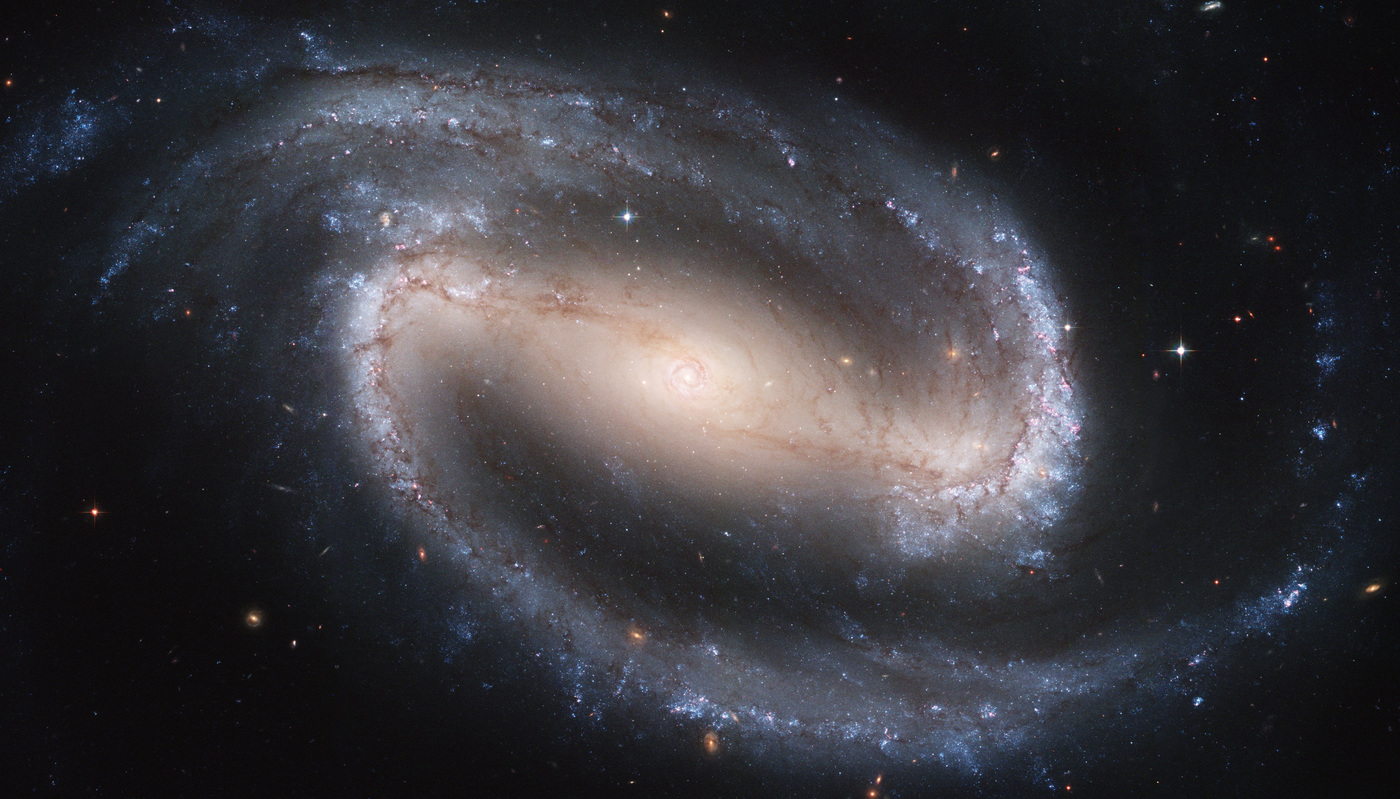
\includegraphics[width=0.99\columnwidth]{images/NGC1300.jpg}\caption{Спиральная галактика (<<туманность>>) с перемычкой (NGC 1300)}\end{figure}}
\vs p015 5:6 \li{4.}\bibemph{Центробежные планетарные дочери}. На определённых стадиях своего развития и в случае значительного увеличения частоты вращения, огромные солнца начинают выбрасывать в больших количествах материю, впоследствии соединяющуюся в небольшие миры, которые продолжают обращаться вокруг материнского солнца.
\vs p015 5:7 \li{5.}\bibemph{Сферы гравитационной недостаточности}. Существует критический предел размера отдельных звёзд. Если, достигнув такого предела, солнце не замедляет своего вращения, оно обречено на расщепление; происходит деление солнца, и рождается новая двойная звезда этой разновидности. В результате такого гигантского разрушения впоследствии могут образоваться многочисленные малые планеты.
\vs p015 5:8 \li{6.}\bibemph{Звёзды, образовавшиеся в результате сжатия} [\bibemph{Contractural Stars}]. В малых системах самая большая внешняя планета иногда притягивает к себе соседние миры, в то время как планеты, близко расположенные к солнцу, начинают своё терминальное падение\fnst{То есть падение на центральную звезду, которое завершает их существование в качестве планет.}. В случае вашей солнечной системы такой конец означал бы, что четыре внутренних планеты были бы поглощены солнцем, в то время как крупнейшая планета~--- Юпитер~--- сильно увеличилась бы за счёт захвата остальных миров. Такой конец солнечной системы привёл бы к образованию двух соседних, но неравных солнц, как одного из типов образования двойной звезды. Такие катастрофы случаются нечасто, за исключением периферии звёздных скоплений сверхвселенной.
\vs p015 5:9 \li{7.}\bibemph{Кумулятивные сферы}\fnst{То есть возникающие за счёт накопления~--- аккумуляции~--- материи.}. Из огромного количества материи, циркулирующей в пространстве, могут медленно накапливаться маленькие планеты. Они растут за счёт метеорной аккреции\fnst{В астрофизике под <<аккрецией>> понимают захват (обычно гравитационный) вещества каким\hyp{}либо массивным телом, например: аккреция газа нейтронной звездой с поверхности обычной звезды\hyp{}компаньона.} и незначительных столкновений. В определённых секторах пространства условия благоприятствуют таким формам планетарного рождения. Многие обитаемые миры имели такое происхождение.
\vs p015 5:10 Некоторые плотные тёмные острова являются прямым результатом аккреции преобразующейся в пространстве энергии. Другая группа таких тёмных островов возникла в результате скопления огромного количества холодной материи~--- циркулирующих в пространстве осколков и метеоров. Такие скопления материи никогда не были горячими и, за исключением плотности, по составу очень похожи на Урантию.
\vs p015 5:11 \li{8.}\bibemph{Выгоревшие солнца}. Некоторые из тёмных островов пространства~--- это выгоревшие изолированные солнца, излучившие всю доступную пространственную энергию. Такие организованные единицы материи приближаются к полной конденсации, почти полному затвердеванию; и потребуются многие эпохи для того, чтобы такие огромные массы сверхплотной материи могли перезарядиться в контурах пространства и подготовиться к новым циклам функционирования во вселенной после столкновения или другого возрождающего к жизни космического события.
\vs p015 5:12 \li{9.}\bibemph{Коллизионные сферы}\fnst{От лат. collisio: <<столкновение>>.}. В областях более плотного скопления столкновения~--- не редкость. Такое астрономическое перестраивание сопровождается колоссальными изменениями энергии и преобразованиями материи. Особенно столкновения, в которых участвуют потухшие [dead] солнца, вызывают широкомасштабные флуктуации энергии. Возникающие после столкновения обломки часто образуют материальные ядра для последующего формирования планетарных тел, приспособленных для обитания смертных.
\vs p015 5:13 \li{10.}\bibemph{Архитектурные миры}. Это миры, которые построены в соответствии с планами и особенностями для некоторой специальной цели, такие как Спасоград, столица вашей локальной вселенной, и Уверса, место пребывания правительства нашей сверхвселенной.
\vs p015 5:14 \pc Существует множество других методов эволюции солнц и отделения планет, но именно с помощью вышеизложенных методов возникает подавляющее большинство звёздных систем и планетарных семейств. Для описания всего разнообразия методов, задействованных в звёздных метаморфозах и эволюции планет, потребовалось бы рассказать о почти 100 различных способах солнцеобразования и возникновения планет. Ваши астрономы [star students], сканируя небеса, обнаружат явления, указывающие на все эти способы звёздной эволюции, но им редко удастся заметить признаки формирования тех небольших несветящихся скоплений материи, которые служат в качестве обитаемых планет,~--- самых важных из многочисленных материальных творений\fnst{Первая планета, находящаяся за пределами Солнечной системы (<<экзопланета>>), была открыта в 1988 году, и с тех пор их число удваивается примерно каждые 27 месяцев. По состоянию на 9~мая 2021 года подтверждено существование 4723 экзопланет в 3493 планетных системах, из которых в 773 имеется более одной планеты.}.
\usection{СФЕРЫ ПРОСТРАНСТВА}
\vs p015 6:1 Независимо от происхождения, различные сферы пространства можно разделить на следующие основные подразделения:
\vs p015 6:2 \li{1.}Солнца~--- звёзды пространства.
\vs p015 6:3 \li{2.}Тёмные острова пространства.
\vs p015 6:4 \li{3.}Малые тела пространства\fnst{Или <<космические тела>>.}~--- кометы, метеоры и планетезимали.
\vs p015 6:5 \li{4.}Планеты, включая обитаемые миры.
\vs p015 6:6 \li{5.}Архитектурные сферы~--- специально созданные миры.
\vs p015 6:7 \pc За исключением архитектурных сфер, все космические тела имеют эволюционное происхождение, эволюционное в том смысле, что они не появились в результате прямого акта Божества; и в том, что созидательные акты Бога были раскрыты посредством время\hyp{}пространственного метода через действия многих созданных и возникших разумных существ Божества.
\vs p015 6:8 \pc \bibemph{Солнца}. Это звёзды пространства на всех различных стадиях их существования. Одни из них~--- одиночные эволюционирующие системы в пространстве; другие представляют собой двойные звёзды, сжимающиеся или исчезающие планетарные системы. Звёзды пространства существуют не менее чем в тысяче различных состояний и стадий. Вы знакомы с солнцами, которые излучают свет, сопровождаемый теплом; но существуют солнца, которые светят без тепла.
\vs p015 6:9 Триллионы и триллионы лет, в течение которых обычное солнце будет продолжать выделять тепло и свет, хорошо иллюстрируют колоссальный запас энергии, который содержится в каждой единице материи. Фактическая энергия, запасённая в этих невидимых частицах физической материи, почти невообразима. И почти вся эта энергия под воздействием огромного теплового давления и связанной с этим энергетической активностью, преобладающей внутри пылающих солнц, выделяется в виде света. Другие условия позволяют этим солнцам преобразовывать и излучать значительную часть той энергии пространства, которая достигает их по установленным пространственным контурам. Многие фазы физической энергии и все формы материи притягиваются и впоследствии распределяются солнечными генераторами. Таким образом, солнца служат в качестве локальных ускорителей циркуляции энергии, действуя как станции автоматического регулирования мощи.
\vs p015 6:10 Сверхвселенная Орвонтон освещается и обогревается более чем десятью триллионами пылающих солнц. Эти солнца~--- звёзды доступной вашему обозрению астрономической системы. Более двух триллионов солнц слишком далеки и слишком малы, чтобы быть видимыми с Урантии. Но в главной вселенной столько же солнц, сколько стаканов воды в океанах вашего мира\fnst{В океанах Урантии примерно $10^{21}$ стаканов воды, а в нашей Галактике около $10^{11}$ звёзд. Следовательно, главная вселенная содержит приблизительно десять миллиардов галактик, размером с Млечный Путь.}.
\vs p015 6:11 \pc \bibemph{Тёмные острова пространства}. Это потухшие солнца и другие крупные скопления материи, лишённые света и тепла. Тёмные острова иногда обладают огромной массой и оказывают сильное влияние на равновесие во вселенной и на управление энергией. Плотность некоторых из этих больших масс почти невероятна. И эта огромная концентрация массы позволяет тёмным островам действовать в качестве мощного балансира, удерживая в надёжной узде большие соседние с ними системы. Они поддерживают гравитационный баланс мощи во многих созвездиях; многие физические системы, которым в противном случае грозило бы быстрое погружение в соседние солнца и разрушение, надёжно удерживаются гравитационным охватом этих тёмных островов\hyp{}хранителей. Именно благодаря этой функции мы можем точно определять их местонахождение. Мы измерили гравитационное притяжение светящихся тел, что позволяет вычислить точный размер и расположение тёмных островов пространства, столь эффективно поддерживающих устойчивость данной системы на её пути.
\vs p015 6:12 \pc \bibemph{Малые тела пространства}. Метеоры и другие мелкие частицы материи, циркулирующие и эволюционирующие в пространстве, составляют огромную совокупность энергии и материальной субстанции.
\vs p015 6:13 Многие кометы~--- это неустановившееся, неуправляемое [wild] потомство солнечных материнских дисков, постепенно переходящее под контроль центрального управляющего солнца. Кометы имеют также и различные другие виды происхождения. Хвост кометы направлен в противоположную сторону от притягивающего тела или солнца из\hyp{}за электрической реакции его сильно разрежённых газов и фактического давления света и других энергий, излучаемых солнцем. Это явление служит одним из убедительных доказательств реальности света и связанных с ним энергий; оно демонстрирует то, что свет имеет вес. Свет~--- это реальная субстанция, а не просто волны гипотетического эфира.
\vs p015 6:14 \pc \bibemph{Планеты}. Это более крупные скопления материи, движущиеся по орбите вокруг солнца или другого космического тела; они варьируются по размеру от планетезималей до огромных газообразных, жидких или твёрдых сфер. Холодные миры, построенные в результате скопления летающего в пространстве вещества, становятся наиболее идеальными планетами для разумных обитателей, когда оказываются в правильной взаимосвязи с ближайшим солнцем. Потухшие солнца, как правило, не приспособлены для жизни; они обычно слишком далеки от живых пылающих солнц и, кроме того, слишком массивны; гравитация на их поверхности огромна.
\vs p015 6:15 В вашей сверхвселенной менее чем одна из сорока холодных планет пригодна для обитания существами вашей категории. И конечно, сверхгорячие солнца и холодные отдалённые миры непригодны для высших форм жизни. В вашей солнечной системе только три планеты\fnst{Две другие планеты, пригодные для обитания в Солнечной системе: Марс и Венера. См.\,\cite{Eddington1}, стр.\,170.} в настоящее время пригодны для жизни. Урантия по своему размеру, плотности и местоположению во многих отношениях идеальна для обитания человека.
\vs p015 6:16 Законы поведения физической энергии в основном универсальны, но местные влияния связаны с физическими условиями, преобладающими на отдельных планетах и в локальных системах. Бесчисленные миры пространства характеризует почти бесконечное разнообразие жизни созданий и других живых проявлений. Однако есть определённые точки сходства в группе миров, объединённых в одну систему, а также существует вселенская модель разумной жизни. Существует физическая взаимосвязь планетарных систем, принадлежащих одному физическому контуру и тесно следующих друг за другом в бесконечном движении по кругу вселенных.
\usection{АРХИТЕКТУРНЫЕ СФЕРЫ}
\vs p015 7:1 Правительство каждой сверхвселенной осуществляет своё руководство, находясь рядом с центром эволюционных вселенных своего сегмента пространства, и занимает специально созданный мир, населённый аккредитованными личностями. Эти столичные миры представляют собой архитектурные сферы~--- тела пространства, специально сконструированные для особой цели. Хотя эти сферы и пользуются светом близлежащих солнц, освещаются и обогреваются они независимо. Каждая имеет солнце, дающее свет без тепла, подобно спутникам Рая, и обогревается за счёт циркуляции определённых энергетических потоков около поверхности сферы. Эти столичные миры принадлежат к одной из крупнейших систем, расположенных вблизи астрономического центра соответствующих сверхвселенных.
\vs p015 7:2 \pc Время в столицах сверхвселенных стандартизировано. Стандартный день сверхвселенной Орвонтон равен почти 30 дням времени Урантии, а год Орвонтона равен 100 стандартным дням. Этот год Уверсы является стандартом для седьмой сверхвселенной, и он на 22 минуты короче 3\,000 дней урантийского времени, что составляет примерно 8,2 ваших лет.
\vs p015 7:3 \pc Столичные миры семи сверхвселенных сопричастны природе и величию Рая, их центральному образцу совершенства. В действительности все столичные миры раеподобны [paradisiacal]. Это поистине небесные обители, и они увеличиваются в материальных размерах, моронтийной красоте и духовной славе от Иерусема до центрального Острова. И все спутники столичных миров также являются архитектурными сферами.
\vs p015 7:4 В различных столичных мирах представлена каждая фаза материального и духовного творения. Все виды материальных, моронтийных и духовных существ чувствуют себя как дома на этих вселенских мирах встреч. По мере восхождения во вселенной, переходя от материальных миров к духовным, смертные никогда не теряют восприятия и наслаждения от своих прежних уровней существования.
\vs p015 7:5 \pc \bibemph{Иерусем,} столица вашей локальной системы Сатания, имеет семь миров переходной культуры, каждый из которых окружён семью спутниками, среди которых семь обительских миров моронтийного заключения\fnst{Использованное здесь английское слово \bibemph{detention} означает <<тюремное заключение, лишение свободы>>. Семь обительских миров являются местами временного заключения: свобода действий и передвижений бывших смертных ограничена до тех пор, пока истинные мотивы души восходящего смертного не будут установлены окончательно, то есть до момента слияния с духом Отца.},~--- первого места пребывания человека после смерти. Термин <<небеса>>, как он использовался на Урантии, иногда обозначал эти семь обительских миров; первый обительский мир назывался первым небом и так далее до седьмого.
\vs p015 7:6 \pc \bibemph{Эденция,} столица вашего созвездия Норлатиадек, имеет 70 спутников культуры социализации и воспитания, где идущие по пути восхождения пребывают после завершения иерусемского режима мобилизации, объединения и реализации личности.
\vs p015 7:7 \pc \bibemph{Спасоград,} столица вашей локальной вселенной Небадон, окружён 10 группами университетов по 49 сфер в каждой. Здесь человек одухотворяется после своей социализации в созвездии.
\vs p015 7:8 \pc \bibemph{Уминор третий,} столица вашего малого сектора Энса, окружён семью сферами высших физических исследований восходящей жизни.
\vs p015 7:9 \pc \bibemph{Умажор\fnst{Буква <<У>> в названиях столиц малого и большого сектора происходит, вероятно, от названия сверхвселенной \textbf{У}верса. А окончания -минор и -мажор свидетельствуют о том, что, начиная с уровня малого сектора, восходящему созданию уже должен становится ясен \bibemph{музыкальный} смысл всего пути восхождения.} пятый,} столица вашего большого сектора Спландон, окружён 70 сферами развивающей интеллектуальной подготовки сверхвселенной.
\vs p015 7:10 \pc \bibemph{Уверса\fnst{Слово <<Уверса>>, возможно, синтезировано специально для английского текста Откровения следующим образом: <<U>>~--- 21\hyp{}я буква латинского алфавита, используемого в английском языке, находится на последнем месте седьмой тройки: 1$=$(A,B,C), 2$=$(D,E,F),\ldots, 7$=$(S,T,U). Окончание -верса, в таком случае, есть указание на то, что, когда последняя нота цикла будет сыграна, мы <<возвращаемся>> (лат. versamus) к Отцу. В русском алфавите <<у>> тоже занимает последнее место седьмой тройки. Следовательно, русифицированное название столицы нашей сверхвселенной может быть синтезировано в форме <<Увозврат>> или <<Увращение>>.},} столица вашей сверхвселенной Орвонтон, непосредственно окружена 7 высшими университетами углублённой духовной подготовки восходящих волевых созданий. Каждая из этих семи групп удивительных сфер состоит из 70 специализированных миров, содержащих тысячи и тысячи разнообразных учреждений и организаций, посвящённых вселенскому образованию и культуре духа, где пилигримы времени переобучаются и переэкзаменуются перед своим долгим полётом к Хавоне. Прибывающие пилигримы времени всегда принимаются на этих вспомогательных мирах, но отбывающие выпускники всегда отправляются в Хавону прямо с берегов Уверсы.
\vs p015 7:11 Уверса является духовным и административным центром примерно одного триллиона обитаемых или пригодных для обитания миров. Слава, величие и совершенство столицы Орвонтона превосходит любое из чудес время\hyp{}пространственных творений.
\vs p015 7:12 \pc Если бы все спроектированные локальные вселенные и их составные части уже существовали, то в семи сверхвселенных было бы чуть менее 500 миллиардов\fnst{Точное число~--- 453\,313\,764\,407. Оно вычисляется следующим образом: 7\dt(1+7\dt70+10\dt(70+1)+1000\dt(7+1)+100\,000\dt647\,591).} архитектурных миров.
\usection{КОНТРОЛЬ И РЕГУЛИРОВАНИЕ ЭНЕРГИИ}
\vs p015 8:1 Столичные сферы сверхвселенных сконструированы так, что могут функционировать как эффективные регуляторы мощи\hyp{}энергии для соответствующих секторов, выступая в качестве фокальных точек для направления энергии в составляющие их локальные вселенные. Они оказывают мощное влияние на баланс и управление физическими энергиями, циркулирующими в организованном пространстве.
\vs p015 8:2 Дальнейшие регулирующие функции выполняются центрами мощи и физическими регуляторами, живыми и полуживыми разумными сущностями, созданными для этой конкретной цели. Эти центры мощи и регуляторы трудны для понимания; низшие категории неспособны к принятию волевых решений, они не обладают волей, они не выбирают, их функции очень разумны, но, по\hyp{}видимому, автоматичны и свойственны их высокоспециализированной организации. Центры мощи и физические регуляторы сверхвселенных принимают на себя руководство и частичный контроль над 30 энергетическими системами, составляющими область гравиты. Чтобы завершить окружение сверхвселенной контурами физической энергии, управляемыми центрами мощи Уверсы, требуется немногим более 968\,000\,000 лет.
\vs p015 8:3 \pc Развивающаяся энергия обладает субстанцией; она имеет вес, хотя вес всегда относителен и зависит от скорости обращения, массы и антигравитации. Масса в материи стремится замедлять скорость в энергии\fnst{Если рассматривать массу покоя $m$ как канонический импульс $p^5=m$ в 5\hyp{}мерном пространстве, сопряжённый собственному времени $\tau$ (или интервалу, играющему роль действия для свободной частицы), то это иначе бессмысленное утверждение становится почти понятным. См.\,\bibref[23:3.2]{p023 3:3}.}; а присутствующая повсюду скорость энергии представляет собой: начальное значение скорости минус замедление, вызванное массой во время перемещения, плюс регулирующую функцию живых регуляторов энергии сверхвселенной и физическое влияние близлежащих сильно нагретых или сильно заряженных тел.
\vs p015 8:4 Универсальный план поддержания равновесия между материей и энергией требует постоянного создания и разрушения малых материальных единиц. Управляющие Вселенской Мощью обладают способностью уплотнять и удерживать или расширять и высвобождать различные количества энергии.
\vs p015 8:5 При достаточно продолжительном замедляющем влиянии гравитация в конце концов преобразовала бы всю энергию в материю, если бы не два фактора: во\hyp{}первых, антигравитационное влияние регуляторов энергии и, во\hyp{}вторых, тенденция к распаду организованной материи при определённых условиях, встречающихся в очень горячих звёздах, и при особых условиях в пространстве вблизи высокоэнергетических холодных тел из сжатой [condensed] материи.
\vs p015 8:6 Когда масса становится сверхагрегированной и угрожает нарушить баланс энергии, истощить контуры физической мощи, вмешиваются физические регуляторы\fnst{Получается, что возникновению гравитационных сингулярностей (т.н. <<чёрных дыр>>) препятствует либо личное вмешательство физических регуляторов, либо случайные столкновения коллапсаров.}, если только дальнейшая тенденция гравитации к чрезмерной материализации энергии не прекратится из\hyp{}за случайного столкновения между мёртвыми гигантами космоса, тем самым мгновенно рассеивая кумулятивные скопления гравитации. В случае таких столкновений огромные массы материи внезапно превращаются в редчайшую форму энергии, и борьба за всеобщее равновесие начинается снова. В итоге более крупные физические системы стабилизируются, становятся физически устойчивыми и включаются в сбалансированные и установившиеся контуры сверхвселенных. После этого события в таких устойчивых системах больше не происходит столкновений или других разрушительных катастроф.
\vs p015 8:7 В периоды избытка энергии наблюдаются энергетические возмущения и тепловые флуктуации, сопровождаемые электрическими феноменами. В периоды недостатка энергии возрастают тенденции материи к накоплению, уплотнению и выходу из\hyp{}под контроля в более тонко сбалансированных контурах; возникающие вследствие этого приливные или коллизионные изменения быстро восстанавливают баланс между циркулирующей энергией и буквально более стабильной материей. Прогнозирование и понимание такого вероятного поведения пылающих солнц и тёмных островов пространства~--- одна из задач небесных наблюдателей звёзд.
\vs p015 8:8 Мы способны распознать большинство законов, управляющих вселенским равновесием, и предсказать многое, относящееся к стабильности вселенной. На практике наши прогнозы надёжны, но мы постоянно сталкиваемся с определёнными силами, которые не полностью подчиняются известным нам законам управления энергией и поведения материи. По мере нашего продвижения из Рая наружу во вселенные, предсказуемость всех физических явлений затрудняется. Выходя за пределы личного управления Райских Правителей, мы сталкиваемся с растущей неспособностью производить расчёты в соответствии с установленными стандартами и опытом, приобретённым при наблюдениях, имеющих отношение исключительно к физическим явлениям ближайших астрономических систем. Даже в областях семи сверхвселенных мы живём в среде силовых воздействий и энергетических реакций, наполняющих все наши сферы и простирающихся в едином равновесии во все регионы внешнего пространства.
\vs p015 8:9 Чем дальше мы идём, тем больше вероятность столкновения с изменчивыми и непредсказуемыми явлениями, которые столь безошибочно характерны для непостижимого присутствия\hyp{}действия Абсолютов и эмпирических Божеств. И эти явления должны указывать на некий универсальный сверхконтроль над всеми вещами.
\vs p015 8:10 Сверхвселенная Орвонтон в настоящее время, очевидно, останавливается; внешние вселенные, кажется, заряжаются для беспрецедентной будущей активности; центральная вселенная Хавона вечно стабилизирована. Гравитация и отсутствие тепла (холод) организуют и скрепляют материю; тепло и антигравитация разрушают материю и рассеивают энергию. Живые управляющие мощью и организаторы силы~--- вот секрет особого управления и разумного руководства бесконечными метаморфозами создания, разрушения и воссоздания вселенных. Туманности могут рассеиваться, солнца выгорать, системы исчезать, планеты погибать, но вселенные не останавливаются.
\usection{КОНТУРЫ СВЕРХВСЕЛЕННЫХ}
\vs p015 9:1 Всеобщие контуры Рая фактически пронизывают области семи сверхвселенных. К этим контурам присутствия относятся: гравитация личности Всеобщего Отца, духовная гравитация Вечного Сына, гравитация разума Совместного Вершителя и материальная гравитация вечного Острова.
\vs p015 9:2 В дополнение к всеобщим контурам Рая и к присутствию\hyp{}действиям Абсолютов и эмпирических Божеств, на пространственном уровне сверхвселенных функционируют только два вида энергетических контуров или распределения мощи: контуры сверхвселенных и контуры локальных вселенных.
\vs p015 9:3 \pc \bibemph{Контуры сверхвселенных:}
\vs p015 9:4 \li{1.}Объединяющий контур разума одного из Семи Главных Духов Рая. Такой контур космического разума ограничен одной сверхвселенной.
\vs p015 9:5 \li{2.}Контур отражательного служения семи Отражательных Духов в каждой сверхвселенной.
\vs p015 9:6 \li{3.}Секретные контуры Таинственных Мониторов, определённым образом взаимосвязанные и направляемые через Божеград к Всеобщему Отцу на Рае.
\vs p015 9:7 \li{4.}Контур общения Вечного Сына со своими Райскими Сынами.
\vs p015 9:8 \li{5.}Молниеносное присутствие Бесконечного Духа.
\vs p015 9:9 \li{6.}Трансляции Рая, пространственные сообщения Хавоны.
\vs p015 9:10 \li{7.}Энергетические контуры центров мощи и физических регуляторов.
\vs p015 9:11 \pc \bibemph{Контуры локальных вселенных:}
\vs p015 9:12 \li{1.}Дух посвящения Райских Сынов, Утешитель миров посвящения. Дух Истины, дух Михаила на Урантии.
\vs p015 9:13 \li{2.}Контур Божественных Помощниц, Материнских Духов локальных вселенных, Святой Дух вашего мира.
\vs p015 9:14 \li{3.}Контур служения разума локальной вселенной, включающий разнообразно функционирующее присутствие адъютантов разумо\hyp{}духов\fnst{Выбирая термин для описания этих удивительных существ, я решил буквально копировать английскую фразу adjutant mind\hyp{}spirits, вместо более привычно звучащего варианта <<духов помощников разума>>, и сделал это по следующей причине. Эти существа, с практически автоматической деятельностью которых мы встречаемся при каждом биении сердца и при каждом вдохе и выдохе, не являются духами в смысле возможности личностного контакта с ними со стороны человека. Они вполне соответствуют семи т.н. чакрам эзотерических учений, и проще всего их визуализировать в виде энергетических центров или вихрей, сфокусированных в разных частях тела. На самом деле их видимые (не обычным зрением, разумеется) проявления в виде <<чакр>> являются лишь проекцией с уровня материального разума на модель нашего тела, создаваемую нашим же разумом, т.е. на ту часть материальной Вселенной, которую мы условно воспринимаем как собственное смертное тело. Уровень функционирования материального разума, соответствующий каналам адъютантов, в точности соответствует уровню восприятия Вселенской космической семьи как чего\hyp{}то отдельного от собственного тела и разума. Переход на моронтийный уровень функционирования разума, лежащий \bibemph{над} семью адъютантами, даже чисто геометрически (5\hyp{}е измерение есть собственное время частицы, параметризующее её существование отдельно от других частиц,~--- <<псевдосознание>>,~--- т.е., начиная с 5\hyp{}го измерения, Вселенная представляет собой отдельное многообразие для каждой частицы, и возможность сосуществования многих частиц означает изоморфизм всех этих многообразий) подразумевает гармоничное соответствие (но не обязательно отождествление, как и в нашем теле левая и правая рука работают в гармонии друг с другом, но не отождествляются) с другими <<элементами>> космической семьи, достигшими того же уровня восприятия реальности. На ту же самую нелокальность и нелокализуемость материи (а тем более разума) указывают соображения из квантовой механики. Например: изменение \bibemph{квантовых} траекторий (рассчитанных по квантовой теории движения де Бройля и Бома) частиц, летящих на потенциальный барьер, \bibemph{до} достижения барьера, а также смещение интерференционной картины электронных пучков, пролетающих в области нулевого магнитного поля, но отличного от нуля векторного потенциала $\mathbf{A(r)}$ (эффект Ааронова\hyp{}Бома).}.
\vs p015 9:15 \pc Когда в локальной вселенной проявляется такая духовная гармония, что её индивидуальные и объединённые контуры становятся неотличимыми от контуров сверхвселенной, когда эта идентичность функций и единство служения действительно преобладают, тогда локальная вселенная немедленно переходит в установившиеся контуры света и жизни, сразу получая право на вступление в духовную конфедерацию союза сверхтворения, ставшего совершенным. Условия для приёма в советы От Века Древних и членство в сверхвселенской конфедерации следующие:
\vs p015 9:16 \li{1.}\bibemph{Физическая стабильность}. Звёзды и планеты локальной вселенной должны находиться в равновесии; периоды непосредственных звёздных трансформаций должны быть завершены. Вселенная должна продолжать движение по ясно проложенному пути; её орбита должна стать надёжно и окончательно установившейся.
\vs p015 9:17 \li{2.}\bibemph{Духовная преданность}. Должно существовать состояние всеобщего признания и преданности Суверенному Сыну Бога, руководящему делами такой локальной вселенной. Должно наступить состояние гармоничного сотрудничества между отдельными планетами, системами и созвездиями всей локальной вселенной.
\vs p015 9:18 \pc Ваша локальная вселенная даже не принадлежит к категории физически устойчивых образований сверхвселенной, не говоря уже о членстве в признанной духовной семье сверхправления. Хотя Небадон ещё не имеет своего представительства на Уверсе, время от времени нас, входящих в состав правительства сверхвселенной, посылают в его миры с особыми миссиями, как и я прибыл на Урантию прямо с Уверсы. Мы оказываем всевозможную помощь вашим руководителям и правителям в решении их сложных проблем; мы очень хотим видеть вашу вселенную полностью соответствующей условиям для принятия в объединённые творения семьи сверхвселенной.
\usection{ПРАВИТЕЛИ СВЕРХВСЕЛЕННЫХ}
\vs p015 10:1 Столицы сверхвселенных~--- это резиденции высшего духовного правительства областей времени и пространства. Исполнительной ветвью сверхправительства, берущей начало в Советах Троицы, непосредственно руководит один из Семи Главных Духов верховного надзора, существ, которые обладают полномочиями Рая и управляют сверхвселенными через Семь Верховных Исполнителей, располагающихся на семи особых мирах Бесконечного Духа~--- самых внешних спутниках Рая.
\vs p015 10:2 Столицы сверхвселенных~--- это места пребывания Отражательных Духов и Помощников Отражательного Изображения. С этой промежуточной позиции эти восхитительные существа совершают свои потрясающие отражательные операции, таким образом служа как вышестоящей центральной вселенной, так и нижестоящим локальным вселенным.
\vs p015 10:3 \pc Каждую сверхвселенную возглавляют трое От Века Древних, совместные главные руководители сверхправительства. Персонал исполнительной ветви сверхвселенского правительства состоит из семи различных групп:
\vs p015 10:4 \li{1.}От Века Древние.
\vs p015 10:5 \li{2.}Совершенствователи Мудрости.
\vs p015 10:6 \li{3.}Божественные Советники.
\vs p015 10:7 \li{4.}Всеобщие Цензоры.
\vs p015 10:8 \li{5.}Могущественные Посланники.
\vs p015 10:9 \li{6.}Облечённые Высокой Властью.
\vs p015 10:10 \li{7.}Не Имеющие Имени и Номера\fnst{Или <<Числа>> (англ. Those without Name and Number).}.
\vs p015 10:11 \pc Трём От Века Древним непосредственно помогает корпус из миллиарда Совершенствователей Мудрости, с которыми связаны три миллиарда Божественных Советников. К каждой администрации сверхвселенной прикреплён миллиард Всеобщих Цензоров. Эти три группы~--- Равноправные Троичные Личности, берущие происхождение непосредственно и божественно в Райской Троице.
\vs p015 10:12 Остальные три категории~--- Могущественные Посланники, Облечённые Высокой Властью и Не Имеющие Имени и Номера~--- прославленные восходящие смертные. К первой из этих категорий относятся прошедшие режим восхождения и Хавону во дни Грандфанды. Достигнув Рая, они были собраны в Корпус Завершения, объяты Райской Троицей и впоследствии назначены на божественное служение в помощь От Века Древним. Как класс, эти три категории известны как Тринитизованные Сыны Достижения; они имеют двойственное происхождение, но теперь служат Троице. Таким образом исполнительная власть правительства сверхвселенной была расширена за счёт прославленных и ставших совершенными детей эволюционных миров.
\vs p015 10:13 Координационный совет сверхвселенной состоит из семи ранее названных исполнительных групп, а также следующих правителей секторов и других региональных надзирателей:
\vs p015 10:14 \li{1)}От Века Совершенных~--- правителей больших секторов сверхвселенной;
\vs p015 10:15 \li{2)}От Века Недавних~--- руководителей малых секторов сверхвселенной;
\vs p015 10:16 \li{3)}От Века Единых~--- Райских советников правителей локальных вселенных;
\vs p015 10:17 \li{4)}От Века Верных~--- Райских советников Всевышних правителей правительств созвездий;
\vs p015 10:18 \li{5)}Троичных Сынов Учителей~--- в случае, когда они служат в столице сверхвселенной;
\vs p015 10:19 \li{6)}От Века Вечных~--- в случае, когда они присутствуют в столице сверхвселенной;
\vs p015 10:20 \li{7)}Семи Помощников Отражательного Изображения~--- выразителей семи Отражательных Духов и, через них, представителей Семи Главных Духов Рая.
\vs p015 10:21 \pc Помощники Отражательного Изображения также действуют как представители многочисленных групп существ, имеющих влияние в правительствах сверхвселенных, но в настоящее время по разным причинам не полностью проявляющих свои индивидуальные способности. В эту группу входят: развивающееся сверхвселенское проявление личности Верховного Существа, Безусловные Смотрители Верховного, Условные Наместники Предельного, безымянные связующие отражатели Мажестона и сверхличностные духовные представители Вечного Сына.
\vs p015 10:22 \pc На столичных мирах сверхвселенных почти всегда можно найти представителей всех групп созданных существ. Текущую работу по оказанию помощи в сверхвселенных выполняют могущественные секонафимы и другие члены обширной семьи Бесконечного Духа. В работе этих изумительных центров сверхвселенского управления, контроля, служения и исполнительного правосудия разумные существа всех сфер вселенской жизни объединяются в эффективном служении, мудром управлении, любящей опеке и справедливых судебных решениях.
\vs p015 10:23 Сверхвселенные не имеют взаимных посольских представительств; они полностью изолированы друг от друга. Они знают об общих делах только через Райский информационный центр, поддерживаемый Семью Главными Духами. Их правители трудятся в советах божественной мудрости на благо своих собственных сверхвселенных независимо от того, что происходит в других частях всеобщего творения. Эта изоляция сверхвселенных будет сохраняться до тех пор, пока они не достигнут согласованности благодаря более полной фактуализации личности и полновластия [personality\hyp{}sovereignty] развивающегося эмпирического Верховного Существа.
\usection{СОВЕЩАТЕЛЬНАЯ АССАМБЛЕЯ}
\vs p015 11:1 Именно на таких мирах, как Уверса, встречаются лицом к лицу существа, олицетворяющие автократию совершенства и демократию эволюции. Исполнительная ветвь сверхправительства берёт своё начало в областях совершенства; законодательная ветвь представлена цветом эволюционных вселенных.
\vs p015 11:2 Совещательная ассамблея сверхвселенной ограничена пределами столичного мира. Этот законодательный, или консультативный, совет состоит из семи палат, в каждую из которых локальные вселенные, допущенные в советы сверхвселенной, избирают местного представителя. Эти представители выбираются высшими советами таких локальных вселенных из числа восходящих пилигримов, выпускников Орвонтона, проживающих на Уверсе и аккредитованных для перемещения в Хавону. Средний срок служения составляет около 100 лет стандартного времени сверхвселенной.
\vs p015 11:3 Я никогда не слышал о разногласиях между представителями исполнительной власти Орвонтона и ассамблеей Уверсы. Никогда ещё в истории нашей сверхвселенной совещательный орган не вносил рекомендаций, выполнение которых могло бы вызвать хоть малейшее сомнение у представителей исполнительной власти сверхправительства. Всегда в работе царила совершенная гармония и взаимное согласие; всё это свидетельствует о том, что эволюционные существа действительно могут достичь высот ставшей совершенной мудрости, дающей им право общаться с личностями совершенного происхождения и божественной природы. Присутствие совещательных ассамблей в столицах сверхвселенных раскрывает мудрость и предвещает окончательный триумф всей необъятной эволюционной концепции Всеобщего Отца и его Вечного Сына.
\usection{ВЕРХОВНЫЕ СУДЫ}
\vs p015 12:1 Когда мы говорим об исполнительной и совещательной ветвях правительства Уверсы, вы можете, по аналогии с некоторыми формами гражданского правления Урантии, предположить, что у нас должна быть третья, или судебная, ветвь власти, и это так; но у неё нет отдельного персонала. Состав наших судов следующий: в соответствии с характером и серьёзностью дела председательствует От Века Древний, Совершенствователь Мудрости или Божественный Советник. Свидетельские показания в пользу или против индивидуума, планеты, системы, созвездия или вселенной представляются и интерпретируются Цензорами. Защиту детей времени и эволюционных планет берут на себя Могущественные Посланники, официальные наблюдатели правительства сверхвселенной в локальных вселенных или системах. Позицию высшего правительства представляют Облечённые Высокой Властью. Приговор же обычно формулируется комиссией с переменным числом участников, состоящей в равной степени из Не Имеющих Имени и Номера и группы чутких личностей, избранных от совещательной ассамблеи.
\vs p015 12:2 Суды От Века Древних~--- это высшие апелляционные суды для вынесения решений по духовным вопросам всех вселенных, составляющих сверхвселенную. Суверенные Сыны локальных вселенных обладают верховной властью в своих владениях; они подчиняются сверхправительству ровно настолько, насколько сами добровольно представляют дела на рассмотрение или вынесение решения От Века Древними, за исключением вопросов, связанных с прекращением существования волевых созданий. Мандаты судебного решения берут начало в локальных вселенных, но приговоры, касающиеся прекращения существования волевых созданий, всегда формулируются и исполняются из столицы сверхвселенной. Сыны локальных вселенных могут принять постановление о сохранении [survival] смертного человека, но только От Века Древние могут выносить подлежащее исполнению решение по вопросам вечной жизни и смерти.
\vs p015 12:3 От Века Древние или их коллеги выносят решения по всем вопросам, не требующим судебного разбирательства и предоставления доказательств, и эти судебные решения всегда единодушны. Здесь мы имеем дело с советами совершенства. В постановлениях этих верховных и высочайших судов нет разногласий или мнений меньшинства.
\vs p015 12:4 За некоторыми исключениями, юрисдикция сверхправительства распространяется на всё и на всех в соответствующих владениях. Постановления и решения властей сверхвселенной не подлежат апелляции, поскольку они представляют совпадающие мнения От Века Древних и того Главного Духа, который из Рая руководит предназначением соответствующей сверхвселенной.
\usection{ПРАВИТЕЛЬСТВА СЕКТОРОВ}
\vs p015 13:1 \bibemph{Большой сектор} охватывает примерно одну десятую часть сверхвселенной и состоит из 100 малых секторов, 10\,000 локальных вселенных, около 100\,000\,000\,000 пригодных для обитания миров. Эти большие сектора управляются тремя От Века Совершенными, Верховными Троичными Личностями.
\vs p015 13:2 Суды От Века Совершенных устроены во многом так же, как и суды От Века Древних, за исключением того, что они не выносят духовных судебных решений в отношении миров. Работа этих правительств больших секторов в основном связана с интеллектуальным статусом обширного творения. Большие сектора задерживают, выносят решения, распределяют и сводят в таблицы для передачи в суды От Века Древних все повседневные и административные вопросы сверхвселенской важности, не связанные непосредственно с духовным управлением мирами или с осуществлением планов Райских Правителей по восхождению смертных. Персонал правительства большого сектора ничем не отличается от персонала сверхвселенной.
\vs p015 13:3 Как великолепные спутники Уверсы связаны с вашей окончательной духовной подготовкой к Хавоне, так и 70 спутников Умажора пятого посвящены вашему интеллектуальному обучению и развитию в сверхвселенной. Со всего Орвонтона здесь собираются мудрые существа, неустанно трудящиеся, чтобы подготовить смертных времени к их дальнейшему продвижению по пути вечности. Б\'ольшая часть этого обучения восходящих смертных проводится на 70 учебных мирах.
\vs p015 13:4 \pc Правительства \bibemph{малых секторов} возглавляют трое От Века Недавних. Их администрация занимается в основном физическим управлением, объединением, стабилизацией и повседневным согласованием управления локальными вселенными, составляющими малый сектор. Каждый малый сектор включает до 100 локальных вселенных, 10\,000 созвездий, 1\,000\,000 систем, или около 1\,000\,000\,000 пригодных для обитания миров.
\vs p015 13:5 Центральные миры малых секторов~--- это грандиозные места встреч Главных Физических Регуляторов. Эти столичные миры окружены семью сферами обучения, которые образуют начальные школы сверхвселенной и являются центрами обретения знаний о физическом устройстве и администрации вселенной вселенных.
\vs p015 13:6 Администраторы правительств малых секторов находятся под непосредственной юрисдикцией правителей большого сектора. От Века Недавние получают все сообщения о наблюдениях и координируют все рекомендации, которые поступают в сверхвселенную от От Века Единых, находящихся на сферах столиц локальных вселенных в качестве наблюдателей и советников Троицы, и от От Века Верных, которые аналогично прикреплены к советам Всевышних в столицах созвездий. Все такие сообщения передаются От Века Совершенным на большие сектора для последующей передачи в суды От Века Древних. Так режим Троицы простирается от созвездий локальных вселенных до столицы сверхвселенной. Столицы локальных систем представителей Троицы не имеют.
\usection{ЦЕЛИ СЕМИ СВЕРХВСЕЛЕННЫХ}
\vs p015 14:1 Существует семь основных целей, раскрывающихся в эволюции семи сверхвселенных. Каждая основная цель эволюции сверхвселенной найдёт наиболее полное выражение только в одной из них, и поэтому каждая сверхвселенная обладает особой функцией и уникальной природой.
\vs p015 14:2 Орвонтон, седьмая сверхвселенная, к которой принадлежит ваша локальная вселенная, известна главным образом благодаря огромному и щедрому дарованию милосердного служения смертным миров. Она славится тем особым методом, благодаря которому справедливость торжествует, будучи смягчённой милосердием, и власть побеждает, будучи обусловленной терпением, где добровольно приносятся жертвы времени для обеспечения стабилизации вечности. Орвонтон~--- вселенская демонстрация любви и милосердия.
\vs p015 14:3 Однако очень трудно описать нашу концепцию истинной природы эволюционной цели, разворачивающейся в Орвонтоне, но можно сказать, что здесь, в этом сверхтворении, мы ощущаем, как шесть уникальных целей космической эволюции, проявляемых в шести ассоциированных сверхтворениях, взаимосвязаны в виде единого смысла целого; и именно поэтому мы иногда предполагаем, что в отдалённом будущем развитая и завершённая персонализация Бога Верховного будет править из Уверсы ставшими совершенными семью сверхвселенными во всём эмпирическом величии его грядущей суверенной власти.
\vs p015 14:4 Орвонтон уникален по своей природе и индивидуален по своему предназначению, так же как и каждая из шести связанных с ним сверхвселенных. Однако многое из того, что происходит в Орвонтоне, вам не раскрыто, и многие из этих нераскрытых сторон жизни Орвонтона находят наиболее полное выражение в какой\hyp{}либо другой сверхвселенной. Семь целей эволюции сверхвселенных действуют по всем семи сверхвселенным, но каждое сверхтворение наиболее полно выражает только одну из этих целей. Для б\'ольшего понимания этих целей сверхвселенных следовало бы раскрыть ещё многое из того, что остаётся для вас непонятным, но и тогда вы бы поняли лишь немногое. Весь этот рассказ представляет собой лишь беглый взгляд на огромное творение, частью которого является ваш мир и ваша локальная система.
\vs p015 14:5 \pc Ваш мир называется Урантия, и его номер в планетарной группе, или системе, Сатания~--- 606. Эта система в настоящее время насчитывает 619 обитаемых миров, и ещё более 200 планет благоприятно развиваются, чтобы в будущем стать обитаемыми мирами.
\vs p015 14:6 Столичный мир Сатании называется Иерусем, и это система номер 24 в созвездии Норлатиадек. Ваше созвездие Норлатиадек состоит из 100 локальных систем, а его столичный мир называется Эденция. Норлатиадек числится под номером 70 во вселенной Небадон. Локальная вселенная Небадон состоит из 100 созвездий и имеет столицу, известную как Спасоград. Вселенная Небадон имеет номер 84 в малом секторе Энса.
\vs p015 14:7 Малый сектор Энса состоит из 100 локальных вселенных, и его столица называется Уминор третий. Этот малый сектор числится под номером 3 в большом секторе Спландон. Спландон состоит из 100 малых секторов, а столица его~--- Умажор пятый. Это 5\hyp{}й большой сектор сверхвселенной Орвонтон, 7\hyp{}го сегмента большой вселенной. Так вы можете определить положение вашей планеты в структуре организации и управления вселенной вселенных.
\vs p015 14:8 Номер вашего мира, Урантии, в большой вселенной~--- 5\,342\,482\,337\,666. Это регистрационный номер на Уверсе и на Рае, ваш номер в каталоге обитаемых миров. Я знаю регистрационный номер физической сферы, но он настолько огромен, что не имеет практического значения\fnst{Практическое значение приведённого выше номера 5\,342\,482\,337\,666 в каталоге обитаемых миров, например, состоит в том, что, судя по его величине, из потенциально возможных семи триллионов обитаемых миров более пяти уже стали реальностью.} для смертного разума.
\vs p015 14:9 \pc Ваша планета~--- частица огромного космоса; вы принадлежите к почти бесконечной семье миров, но руководят вашей сферой с такой же точностью и заботятся о ней с такой же любовью, как если бы это был единственный обитаемый мир из всех существующих.
\vsetoff
\vs p015 14:10 [Представлено Всеобщим Цензором из Уверсы]. 
\quizlink
\begin{thebibliography}{100}
\bibitem{Eddington1}
Sir Arthur Stanley Eddington.
{<<The Nature of the Physical World>>.}
{\em Cambridge, England}, 1929.
\bibitem{Baker1}
Robert H. Baker, Ph.D.
{<<The Universe Unfolding: A Story of Man's Increasing Comprehension of the Universe Around Him.>>}
{\em Baltimore: The Williams \&\ Wilkins Company}, 1932.
\bibitem{Barnes1}
Ernest William Barnes.
{<<Scientific Theory and Religion: The World described by Science and its Spiritual interpretation>>.}
{\em Cambridge: At the University Press}, 1933.
\bibitem{Swann1}
W.F.G.~Swann.
{``The Architecture of the Universe''}
{\em New York: The Macmillan Company}, 1934.
\end{thebibliography}

\upaper{16}{СЕМЬ ГЛАВНЫХ ДУХОВ}
\uminitoc{ОТНОШЕНИЕ К ТРИЕДИНОМУ БОЖЕСТВУ}
\uminitoc{ОТНОШЕНИЕ К БЕСКОНЕЧНОМУ ДУХУ}
\uminitoc{ИНДИВИДУАЛЬНОСТЬ И РАЗНООБРАЗИЕ ГЛАВНЫХ ДУХОВ}
\uminitoc{АТРИБУТЫ И ФУНКЦИИ ГЛАВНЫХ ДУХОВ}
\uminitoc{ОТНОШЕНИЕ К СОЗДАНИЯМ}
\uminitoc{КОСМИЧЕСКИЙ РАЗУМ}
\uminitoc{НРАВСТВЕННОСТЬ, ДОБРОДЕТЕЛЬ И ЛИЧНОСТЬ}
\uminitoc{УРАНТИЙСКАЯ ЛИЧНОСТЬ}
\uminitoc{РЕАЛЬНОСТЬ ЧЕЛОВЕЧЕСКОГО СОЗНАНИЯ}
\author{Всеобщий Цензор}
\vs p016 0:1 Семь Главных Духов Рая --- первичные личности Бесконечного Духа. В этом семичастном созидательном акте самоповторения Бесконечный Дух исчерпал комбинаторные возможности, математически свойственные фактическому существованию трёх лиц Божества. Если бы возможно было создать большее число Главных Духов, они были бы созданы, но существует семь, и только семь, возможных комбинаций, присущих трём Божествам. Это объясняет, почему вселенная управляется в семи больших разделах, а число семь является фундаментальным в основе её организации и управления.
\vs p016 0:2 Cемь Главных Духов, таким образом, берут своё начало в следующих семи прообразах, наследуя от них индивидуальные характерные черты:
\vs p016 0:3 \li{1.}Всеобщий Отец.
\vs p016 0:4 \li{2.}Вечный Сын.
\vs p016 0:5 \li{3.}Бесконечный Дух.
\vs p016 0:6 \li{4.}Отец и Сын.
\vs p016 0:7 \li{5.}Отец и Дух.
\vs p016 0:8 \li{6.}Сын и Дух.
\vs p016 0:9 \li{7.}Отец, Сын и Дух.
\vs p016 0:10 \pc Мы очень мало знаем о деятельности Отца и Сына в создании Главных Духов. По всей видимости, они появились в результате личных действий Бесконечного Духа, однако нас со всей определённостью учили, что и Отец, и Сын также участвовали в этом созидательном акте.
\vs p016 0:11 По своей духовной природе и сущности Семь Духов Рая едины, но очень непохожи во всех других аспектах существа, и по оценке их действий в сверхвселенных индивидуальные отличия каждого безошибочно распознаваемы. Все последующие планы семи сегментов большой вселенной --- и даже соответствующих сегментов внешнего пространства --- обусловлены внедуховным разнообразием Семи Главных Духов в верховном и предельном сверхконтроле.
\vs p016 0:12 Главные Духи выполняют множество функций, но в настоящее время основная сфера их деятельности --- центральное руководство семью сверхвселенными. Каждый Главный Дух поддерживает огромный фокально\hyp{}силовой центр, медленно обращающийся вокруг периферии Рая, всегда сохраняя позицию напротив вселенной непосредственного контроля и в Райском фокусе специализированного управления мощью и сегментированного распределения энергии. Радиальные граничные линии любой сверхвселенной действительно сходятся в Райском центре руководящего Главного Духа.
\usection{ОТНОШЕНИЕ К ТРИЕДИНОМУ БОЖЕСТВУ}
\vs p016 1:1 Совместный Создатель --- Бесконечный Дух --- необходим для завершения триединой персонализации неделимого Божества. Эта тройная персонализация Божества является, по сути, семичастной в возможности индивидуального и ассоциативного выражения; поэтому последующий план создания вселенных, населённых разумными и потенциально духовными существами, должным образом выражающими Отца, Сына и Духа, сделал персонализацию Семи Главных Духов неизбежной. Обычно мы говорим о тройной персонализации Божества как об \bibemph{абсолютной неизбежности,} в то же время рассматривая появление Семи Главных Духов как \bibemph{субабсолютную неизбежность}.
\vs p016 1:2 Хотя Семь Главных Духов едва ли выражают \bibemph{трёхчастное} Божество, они являются вечным изображением \bibemph{семичастного} Божества, активными и ассоциативными функциями трёх вечно существующих лиц Божества. С помощью этих Семи Духов, в них и через них, Всеобщий Отец, Вечный Сын или Бесконечный Дух, или любая их парная комбинация, способны действовать как таковые. Когда Отец, Сын и Дух действуют вместе, они могут и действительно функционируют через Главного Духа Номер Семь, но не как Троица. Порознь и совместно Главные Духи представляют любую и все возможные функции Божества, одну или несколько, но не совокупные, не Троицу. Главный Дух Номер Семь лично не функционирует по отношению к Райской Троице, и именно по этой причине он может функционировать \bibemph{лично} от имени Верховного Существа.
\vs p016 1:3 Но когда Семь Главных Духов покидают свои индивидуальные места личной власти и сверхвселенских полномочий и собираются вокруг Совместного Вершителя в триедином присутствии Райского Божества, они коллективно становятся представителями функциональной власти, мудрости и полномочий неделимого Божества --- Троицы --- по отношению к развивающимся вселенным и в них. Такой Райский союз первичного семичастного выражения Божества действительно охватывает, буквально заключает в себе, все атрибуты и отношения трёх вечных Божеств в Верховности и в Предельности. Фактически Семь Главных Духов действительно и сразу охватывают функциональную область Верховного\hyp{}Предельного в главной вселенной и по отношению к ней.
\vs p016 1:4 Насколько мы можем судить, эти Семь Духов связаны с божественной деятельностью трёх вечных лиц Божества; мы не обнаруживаем никакого свидетельства непосредственной связи с функционирующими присутствиями трёх вечных фаз Абсолюта. Во взаимосвязи Главные Духи представляют Райских Божеств в том, что можно приблизительно представить себе как конечную область действия. Эта область может включать многое из того, что является предельным, но \bibemph{не} абсолютным.
\usection{ОТНОШЕНИЕ К БЕСКОНЕЧНОМУ ДУХУ}
\vs p016 2:1 Как Вечный и Изначальный Сын раскрывается через лица постоянно увеличивающегося числа божественных Сынов, так и Бесконечный и Божественный Дух раскрывается через каналы Семи Главных Духов и связанные с ними группы духов. В центре центров Бесконечный Дух доступен, но не все, кто достигает Рая, способны сразу же распознать его личность и дифференцированное присутствие; но все, кто достигает центральной вселенной, могут непосредственно общаться, и действительно общаются, с одним из Семи Главных Духов, возглавляющим ту сверхвселенную, откуда поступил вновь прибывший пилигрим пространства.
\vs p016 2:2 Со вселенной вселенных Райский Отец говорит только через своего Сына, в то же время вместе, он и Сын, действуют только через Бесконечного Духа. Вне Рая и Хавоны Бесконечный Дух \bibemph{говорит} только голосами Семи Главных Духов.
\vs p016 2:3 \pc Бесконечный Дух оказывает влияние \bibemph{личного присутствия} внутри системы Рай\hyp{}Хавона; за её пределами присутствие его личного духа проявляется одним из Семи Главных Духов и через него. Поэтому сверхвселенское присутствие духа Третьего Источника и Центра на любом мире или в любом индивидууме обусловлено уникальной природой руководящего Главного Духа данного сегмента творения. И наоборот, объединённые линии силы духа и разума проходят внутрь, к Третьему Лицу Божества, через Семь Главных Духов.
\vs p016 2:4 \pc Семь Главных Духов коллективно наделяются верховно\hyp{}предельными атрибутами Третьего Источника и Центра. Хотя каждый индивидуально получает этот дар, только коллективно они раскрывают атрибуты всемогущества, всеведения и вездесущности. Поэтому ни один из них не может функционировать универсально; как индивидуумы, в проявлении таких полномочий верховности и предельности, каждый лично ограничен сверхвселенной непосредственного контроля.
\vs p016 2:5 Всё сказанное тебе о божественности и личности Совместного Вершителя в равной и полной мере относится к Семи Главным Духам, которые столь эффективно распределяют Бесконечный Дух по семи сегментам большой вселенной в соответствии со своим божественным даром и согласно своей различной и индивидуально\hyp{}уникальной природе. Поэтому вполне уместно применить к коллективной группе из семи любое или все имена Бесконечного Духа. Вместе они едины с Совместным Создателем на всех субабсолютных уровнях.
\usection{ИНДИВИДУАЛЬНОСТЬ И РАЗНООБРАЗИЕ ГЛАВНЫХ ДУХОВ}
\vs p016 3:1 Семь Главных Духов --- неописуемые существа, но они отчётливо и определённо личностны. У них есть имена, но мы предпочитаем знакомить с ними по номерам. Будучи первичными персонализациями Бесконечного Духа, они родственны друг другу, но как первичные выражения семи возможных комбинаций триединого Божества они существенно отличаются друг от друга по природе, и это различие природы определяет дифференциал их сверхвселенского поведения\fnst{Или <<различие в управлении сверхвселенными>>.}. Эти Семь Главных Духов можно описать следующим образом.
\vs p016 3:2 \bibemph{Главный Дух Номер Один}. Особым образом этот Дух непосредственно представляет Райского Отца. Он --- своеобразное и действенное проявление могущества, любви и мудрости Всеобщего Отца. Он является близким партнёром главы Таинственных Мониторов, того существа, которое возглавляет Коллегию Персонализированных Настройщиков на Дивинингтоне. Во всех ассоциациях Семи Главных Духов от имени Всеобщего Отца всегда говорит Главный Дух Номер Один.
\vs p016 3:3 Этот Дух возглавляет первую сверхвселенную и, неизменно демонстрируя божественную природу первичной персонализации Бесконечного Духа, по всей видимости, по характеру больше похож на Всеобщего Отца. Он всегда поддерживает личную связь с семью Отражательными Духами в столице первой сверхвселенной.
\vs p016 3:4 \pc \bibemph{Главный Дух Номер Два}. Этот Дух --- адекватное изображение несравненной природы и обаятельного характера Вечного Сына, первородного Сына всего творения. Он всегда находится в тесном партнёрстве со всеми категориями Сынов Бога, когда бы ни случилось им оказаться в родной вселенной лично или на радостном конклаве. На всех собраниях Семи Главных Духов он всегда говорит за Вечного Сына и от его имени.
\vs p016 3:5 Этот Дух руководит судьбой второй сверхвселенной и правит этим огромным владением так же, как это делал бы Вечный Сын. Он всегда поддерживает связь с семью Отражательными Духами, расположенными в столице второй сверхвселенной.
\vs p016 3:6 \pc \bibemph{Главный Дух Номер Три}. Этот Дух\hyp{}личность особенно напоминает Бесконечного Духа и руководит передвижениями и работой многих высоких личностей Бесконечного Духа. Он возглавляет их собрания и тесно связан со всеми личностями, которые берут своё исключительное начало от Третьего Источника и Центра. Когда Семь Главных Духов собираются на совет, именно Главный Дух Номер Три всегда говорит от имени Бесконечного Духа.
\vs p016 3:7 Этот Дух отвечает за сверхвселенную номер три и управляет делами этого сегмента во многом так же, как это делал бы Бесконечный Дух. Он всегда поддерживает связь с Отражательными Духами в столице третьей сверхвселенной.
\vs p016 3:8 \pc \bibemph{Главный Дух Номер Четыре}. Разделяя объединённую природу Отца и Сына, этот Главный Дух оказывает определяющее влияние касательно стратегии и тактики Отца\hyp{}Сына в советах Семи Главных Духов. Этот Дух --- главный руководитель и советник тех восходящих существ, которые достигли Бесконечного Духа и, таким образом, стали кандидатами на встречу с Сыном и Отцом. Он поддерживает ту огромную группу личностей, которые происходят от Отца и Сына. Когда необходимо представлять Отца и Сына в ассоциациях Семи Главных Духов, всегда говорит именно Главный Дух Номер Четыре.
\vs p016 3:9 Этот Дух заботится о четвёртом сегменте большой вселенной в соответствии с его уникальной комбинацией атрибутов Всеобщего Отца и Вечного Сына. Он всегда поддерживает личную связь с Отражательными Духами в столице четвёртой сверхвселенной.
\vs p016 3:10 \pc \bibemph{Главный Дух Номер Пять}. Эта божественная личность, в совершенстве сочетающая в себе характер Всеобщего Отца и Бесконечного Духа, является советником огромной группы существ, известных как управляющие мощью, центры мощи и физические регуляторы. Этот Дух также заботится обо всех личностях, происходящих от Отца и Совместного Вершителя. В советах Семи Главных Духов, когда возникает вопрос о точке зрения Отца\hyp{}Духа, всегда говорит именно Главный Дух Номер Пять.
\vs p016 3:11 Этот Дух управляет благополучием пятой сверхвселенной так, как это предполагает объединённый характер действий Всеобщего Отца и Бесконечного Духа. Он всегда поддерживает связь с Отражательными Духами в столице пятой сверхвселенной.
\vs p016 3:12 \pc \bibemph{Главный Дух Номер Шесть}. Это божественное существо, по всей видимости, изображает объединённый характер Вечного Сына и Бесконечного Духа. Всякий раз, когда в центральной вселенной собираются создания, сотворённые совместно Сыном и Духом, их советником выступает именно этот Главный Дух; и всякий раз, когда в советах Семи Главных Духов необходимо говорить совместно за Вечного Сына и Бесконечного Духа, отвечает именно Главный Дух Номер Шесть.
\vs p016 3:13 Этот Дух управляет делами шестой сверхвселенной подобно тому, как это делали бы Вечный Сын и Бесконечный Дух. Он всегда поддерживает связь с Отражательными Духами в столице шестой сверхвселенной.
\vs p016 3:14 \pc \bibemph{Главный Дух Номер Семь}. Возглавляющий седьмую сверхвселенную Дух --- это уникально равное изображение Всеобщего Отца, Вечного Сына и Бесконечного Духа. Седьмой Дух --- наставник и советник всех существ триединого происхождения, является также советником и руководителем всех восходящих пилигримов Хавоны, тех скромных существ, которые достигли чертогов славы [courts of glory] благодаря объединённому служению Отца, Сына и Духа.
\vs p016 3:15 Седьмой Главный Дух не является органическим представителем Райской Троицы; но это известный факт, что его личностная и духовная природа \bibemph{есть} изображение Совместного Вершителя в равных пропорциях трёх бесконечных лиц, чей союз Божеств \bibemph{есть} Райская Троица, и чья функция как таковая \bibemph{есть} источник личностной и духовной природы Бога Верховного. Поэтому Седьмой Главный Дух раскрывает личностное и органическое отношение к духу\hyp{}лицу эволюционирующего Верховного. Поэтому в небесных советах Главных Духов, когда необходимо выбрать совместную личную позицию Отца, Сына и Духа или отобразить духовную позицию Верховного Существа, действует Главный Дух Номер Семь. Таким образом, по своей сущности он становится главой Райского совета Семи Главных Духов.
\vs p016 3:16 Ни один из Семи Духов не является органическим представителем Райской Троицы, но когда они объединяются как семичастное Божество, то этот союз в смысле божества --- не в личностном смысле --- равноценен функциональному уровню, связанному с функциями Троицы. В этом смысле <<Семичастный Дух>> способен функционально объединяться с Райской Троицей. Именно в этом же смысле Главный Дух Номер Семь иногда говорит в подтверждение точки зрения Троицы или, скорее, выражает позицию союза Семичастного Духа относительно позиции союза Трёхчастного Божества, точки зрения Райской Троицы.
\vs p016 3:17 Многочисленные функции Седьмого Главного Духа, таким образом, простираются от объединённого изображения \bibemph{личной природы} Отца, Сына и Духа через представление \bibemph{личной позиции} Бога Верховного до раскрытия \bibemph{позиции божества} Райской Троицы. И в некоторых отношениях этот главенствующий Дух одинаково выражает \bibemph{позиции} Предельного и Верховного\hyp{}Предельного.
\vs p016 3:18 Именно Главный Дух Номер Семь, благодаря своим многочисленным качествам, лично содействует прогрессу кандидатов на восхождение из миров времени в их попытках достичь понимания неделимого Божества Верховности. Такое понимание включает в себя постижение зкзистенциального полновластия Троицы Верховности, так скоординированного с концепцией растущего эмпирического полновластия Верховного Существа, чтобы сделать возможным постижение созданиями единства Верховности. Осознание созданиями этих трёх факторов соответствует хавонскому пониманию реальности Троицы и наделяет пилигримов времени способностью в конечном итоге проникнуть в Троицу, открыть три бесконечных лица Божества.
\vs p016 3:19 Неспособность пилигримов Хавоны полностью найти Бога Верховного компенсируется Седьмым Главным Духом, чья триединая природа таким своеобразным способом раскрывает духовное лицо Верховного. В течение настоящей вселенской эпохи, ввиду невозможности контакта с личностью Верховного, Главный Дух Номер Семь функционирует за Бога восходящих созданий в вопросах личных отношений. Он --- единственное высшее духовное существо, которое все восходящие, несомненно, узн\'ают и отчасти поймут, когда достигнут центров славы.
\vs p016 3:20 Этот Главный Дух всегда поддерживает связь с Отражательными Духами Уверсы --- столицы седьмой сверхвселенной, нашего собственного сегмента творения. Его управление Орвонтоном раскрывает изумительную симметрию согласованного сочетания божественной природы Отца, Сына и Духа.
\usection{АТРИБУТЫ И ФУНКЦИИ ГЛАВНЫХ ДУХОВ}
\vs p016 4:1 Семь Главных Духов есть полное представление Бесконечного Духа эволюционным вселенным. Они представляют Третий Источник и Центр в соотношениях энергии, разума и духа. Хотя они функционируют как координирующие главы всеобщего административного управления Совместного Вершителя, не забывай, что они берут своё начало в созидательных актах Райских Божеств. Буквально верно, что эти Семь Духов являются персонализированной физической мощью, космическим разумом и духовным присутствием триединого Божества, <<Семь Духов Бога, посланных по всей вселенной>>.
\vs p016 4:2 Главные Духи уникальны тем, что они действуют на всех вселенских уровнях реальности, кроме абсолютного. Поэтому они являются эффективными и совершенными руководителями всех фаз административных дел на всех уровнях сверхвселенской активности. Смертному разуму трудно понять очень многое о Главных Духах, потому что их работа является одновременно чрезвычайно специализированной, но всеобъемлющей, столь исключительно материальной и, в то же время, столь изысканно духовной. Эти разносторонние создатели космического разума --- прародители Управляющих Вселенской Мощью и сами являются верховными управляющими огромного и обширного творения духовных созданий.
\vs p016 4:3 Семь Главных Духов являются создателями Управляющих Вселенской Мощью и их помощников --- сущностей, незаменимых для организации, контроля и регулирования физических энергий большой вселенной. И эти же Главные Духи весьма существенно помогают Сынам Создателям в работе формирования и организации локальных вселенных.
\vs p016 4:4 Мы не имеем возможности проследить какую бы то ни было личностную связь между деятельностью Главных Духов, связанной с космической энергией, и силовыми функциями Безусловного Абсолюта. Все энергетические проявления, находящиеся под юрисдикцией Главных Духов, управляются с периферии Рая; они не кажутся связанными напрямую с силовыми феноменами, отождествляемыми с нижней поверхностью Рая.
\vs p016 4:5 Несомненно, что, когда мы сталкиваемся с функциональной активностью различных Руководителей Моронтийной Мощи, мы оказываемся лицом к лицу с определённой нераскрытой деятельностью Главных Духов. Кто, кроме этих прародителей как физических регуляторов, так и духовных помощников, смог бы придумать как соединить и связать материальную и духовную энергии таким образом, чтобы создать несуществующую ранее фазу вселенской реальности --- моронтийную субстанцию и моронтийный разум?
\vs p016 4:6 Значительная часть реальности духовных миров относится к моронтийному типу --- фазе вселенской реальности, совершенно неизвестной на Урантии. Цель существования личности --- духовная, но моронтийные творения всегда занимают промежуточное положение, перекидывая мост через пропасть между материальными мирами происхождения смертных и сверхвселенскими сферами развивающегося духовного статуса. Именно в этой области Главные Духи вносят свой великий вклад в план Райского восхождения человека.
\vs p016 4:7 У Семи Главных Духов есть личные представители, которые действуют по всей большой вселенной; но ввиду того, что подавляющее большинство этих подчинённых существ не связано непосредственно с планом восхождения смертных по пути Райского совершенства, о них почти ничего не раскрыто. Многое, очень многое, из деятельности Семи Главных Духов остаётся скрытым от человеческого понимания, ибо никоим образом не связано непосредственно с вашей задачей Райского восхождения.
\vs p016 4:8 \pc Весьма вероятно, хотя мы и не можем представить конкретных доказательств, что Главный Дух Орвонтона оказывает определённое влияние в следующих сферах деятельности:
\vs p016 4:9 \li{1.}Процедуры зарождения жизни Носителями Жизни локальной вселенной.
\vs p016 4:10 \li{2.}Активация жизни адъютантами разумо\hyp{}духами, дарованными мирам Созидательным Духом локальной вселенной.
\vs p016 4:11 \li{3.}Флуктуации энергетических проявлений, представленные единицами организованной материи, реагирующими на линейную гравитацию.
\vs p016 4:12 \li{4.}Поведение появляющейся энергии, полностью освобождённой от охвата Безусловного Абсолюта, таким образом становящейся восприимчивой к прямому воздействию линейной гравитации и манипуляциям Управляющих Вселенской Мощью и их помощников.
\vs p016 4:13 \li{5.}Дар духа помощи Созидательного Духа локальной вселенной, известного на Урантии как Святой Дух.
\vs p016 4:14 \li{6.}Последующий дар духа посвящения Сынов, называемого на Урантии Утешителем или Духом Истины.
\vs p016 4:15 \li{7.}Механизм отражательности локальных вселенных и сверхвселенной. Многие особенности, связанные с этим необычным феноменом, едва ли могут быть разумно объяснены или рационально поняты без постулирования деятельности Главных Духов в ассоциации с Совместным Вершителем и Верховным Существом.
\vs p016 4:16 \pc Несмотря на нашу неспособность в полной мере понять разнообразные действия Семи Главных Духов, мы уверенны, что в огромной области вселенской деятельности существуют две сферы, к которым они не имеют абсолютно никакого отношения: дар и служение Настройщиков Мыслей и непостижимые функции Безусловного Абсолюта.
\usection{ОТНОШЕНИЕ К СОЗДАНИЯМ}
\vs p016 5:1 
\vs p016 5:2 
\vs p016 5:3 
\vs p016 5:4 
\vs p016 5:5 
\usection{The Cosmic Mind}
\vs p016 6:1 
\vs p016 6:2 
\vs p016 6:3 
\vs p016 6:4 \pc 
\vs p016 6:5 
\vs p016 6:6 
\vs p016 6:7 
\vs p016 6:8 
\vs p016 6:9 \pc 
\vs p016 6:10 \pc 
\vs p016 6:11 
\usection{Morals, Virtue, and Personality}
\vs p016 7:1 
\vs p016 7:2 
\vs p016 7:3 
\vs p016 7:4 
\vs p016 7:5 
\vs p016 7:6 \pc 
\vs p016 7:7 
\vs p016 7:8 \pc 
\vs p016 7:9 \pc 
\vs p016 7:10 
\usection{Urantia Personality}
\vs p016 8:1 
\vs p016 8:2 
\vs p016 8:3 
\vs p016 8:4 
\vs p016 8:5 \pc 
\vs p016 8:6 
\vs p016 8:7 \pc 
\vs p016 8:8 
\vs p016 8:9 
\vs p016 8:10 
\vs p016 8:11 
\vs p016 8:12 
\vs p016 8:13 
\vs p016 8:14 
\vs p016 8:15 \pc 
\vs p016 8:16 
\vs p016 8:17 
\vs p016 8:18 
\vs p016 8:19 \pc 
\usection{Reality of Human Consciousness}
\vs p016 9:1 
\vs p016 9:2 
\vs p016 9:3 
\vs p016 9:4 \pc 
\vs p016 9:5 
\vs p016 9:6 
\vs p016 9:7 \pc 
\vs p016 9:8 
\vs p016 9:9 
\vs p016 9:10 
\vs p016 9:11 
\vs p016 9:12 
\vs p016 9:13 
\vs p016 9:14 \pc 
\vs p016 9:15 
\vsetoff
\vs p016 9:16 
\quizlink

\upaper{17}{СЕМЬ ГРУПП ВЕРХОВНЫХ ДУХОВ}
\uminitoc{СЕМЬ ВЕРХОВНЫХ ИСПОЛНИТЕЛЕЙ}
\uminitoc{МАЖЕСТОН~--- ГЛАВА ОТРАЖАТЕЛЬНОСТИ}
\uminitoc{ОТРАЖАТЕЛЬНЫЕ ДУХИ}
\uminitoc{ПОМОЩНИКИ ОТРАЖАТЕЛЬНОГО ИЗОБРАЖЕНИЯ}
\uminitoc{СЕМЬ ДУХОВ КОНТУРОВ}
\uminitoc{ТВОРЧЕСКИЕ ДУХИ ЛОКАЛЬНЫХ ВСЕЛЕННЫХ}
\uminitoc{АДЪЮТАНТЫ РАЗУМО\hyp{}ДУХИ}
\uminitoc{ФУНКЦИИ ВЕРХОВНЫХ ДУХОВ}
\author{Божественный Советник}
\vs p017 0:1 Семь групп Верховных Духов являются универсальными координирующими руководителями семисегментной администрации большой вселенной. Хотя все они относятся к функциональной семье Бесконечного Духа, следующие три группы обычно классифицируются как дети Райской Троицы:
\vs p017 0:2 \li{1.}Семь Главных Духов.
\vs p017 0:3 \li{2.}Семь Верховных Исполнителей.
\vs p017 0:4 \li{3.}Отражательные Духи.
\vs p017 0:5 \pc Остальные четыре группы возникли в результате созидательных актов Бесконечного Духа или его помощников, обладающих статусом создателей:
\vs p017 0:6 \li{4.}Помощники Отражательного Изображения.
\vs p017 0:7 \li{5.}Семь Духов Контуров.
\vs p017 0:8 \li{6.}Созидательные Духи Локальных Вселенных.
\vs p017 0:9 \li{7.}Адъютанты разумо\hyp{}духи.
\vs p017 0:10 \pc Эти семь категорий известны на Уверсе как семь групп Верховных Духов. Сфера их деятельности простирается от личного присутствия Семи Главных Духов на периферии вечного Острова, охватывая семь Райских спутников Духа, контуры Хавоны, правительства сверхвселенных, управление и надзор за локальными вселенными, вплоть до скромного служения адъютантов в области эволюционного разума на мирах времени и пространства.
\vs p017 0:11 Семь Главных Духов~--- координирующие руководители этой обширной административной сферы. В некоторых вопросах, касающихся административного регулирования организованной физической мощи, энергии разума и неличностного служения духов, они действуют лично и непосредственно, а в других~--- через своих разнообразных партнёров. Во всех вопросах исполнительного характера~--- постановлениях, предписаниях, корректировках и административных решениях~--- Главные Духи действуют в лице Семи Верховных Исполнителей. В центральной вселенной Главные Духи могут функционировать через Семь Духов Контуров Хавоны; на столичных мирах семи сверхвселенных они раскрывают себя через канал Отражательных Духов и действуют через лица От Века Древних, с которыми находятся в личной связи через Помощников Отражательного Изображения.
\vs p017 0:12 Семь Главных Духов напрямую и лично не контактируют с администрацией вселенной ниже уровня судов От Века Древних. Ваша локальная вселенная управляется как часть нашей сверхвселенной Главным Духом Орвонтона, но в отношении исконных жителей Небадона его функция непосредственно осуществляется и лично направляется Созидательным Материнским Духом, пребывающим на Салвингтоне~--- столице вашей локальной вселенной.
\usection{СЕМЬ ВЕРХОВНЫХ ИСПОЛНИТЕЛЕЙ}
\vs p017 1:1 Исполнительные центры Главных Духов занимают семь Райских спутников Бесконечного Духа, обращающихся вокруг центрального Острова между сияющими сферами Вечного Сына и внутренним контуром Хавоны. Эти исполнительные сферы находятся под управлением группы из семи Верховных Исполнителей, тринитизованных Отцом, Сыном и Духом в соответствии с требованиями Семи Главных Духов для существ, способных функционировать в качестве их универсальных представителей.
\vs p017 1:2 Через этих Верховных Исполнителей Главные Духи поддерживают связь с различными отделениями правительств сверхвселенных. Именно они в значительной мере определяют основные существенные направления развития семи сверхвселенных. Они одинаково и божественно совершенны, но обладают отличиями личности. У них нет председательствующего главы; при каждой встрече они избирают одного из своего числа председателем совместного совета. Периодически они путешествуют в Рай для заседаний в совете с Семью Главными Духами.
\vs p017 1:3 \pc Семь Верховных Исполнителей функционируют как административные координаторы большой вселенной; их можно назвать советом управляющих пост\hyp{}Хавонского творения. Они не связаны с внутренними делами Рая и управляют своими ограниченными сферами деятельности Хавоны через Семь Духов Контуров. В остальном сфера их надзора почти не ограничена; они заняты руководством физических, интеллектуальных и духовных дел; они всё видят, всё слышат, всё чувствуют и даже знают всё, что происходит в семи сверхвселенных и в Хавоне.
\vs p017 1:4 Эти Верховные Исполнители не придумывают новые правила и не изменяют вселенские процедуры; они заботятся об исполнении планов божественности, провозглашённых Семью Главными Духами. Они не вмешиваются ни в правление От Века Древних в сверхвселенных, ни в суверенное правление Сынов Создателей в локальных вселенных. Они~--- координирующие исполнители, чья функция заключается в реализации объединённой стратегии всех наделённых должными полномочиями правителей в большой вселенной.
\vs p017 1:5 Каждый из исполнителей и средства его сферы посвящены эффективному руководству одной сверхвселенной. Верховный Исполнитель Номер Один, действующий на исполнительной сфере номер один, полностью занят делами сверхвселенной номер один, и так далее до Верховного Исполнителя Номер Семь, действующего с седьмого Райского спутника Духа и посвятившего свои энергии управлению делами седьмой сверхвселенной. Название этой седьмой сферы~--- Орвонтон, ибо Райские спутники Духа имеют те же названия, что и связанные с ними сверхвселенные; на самом деле сверхвселенные были названы в честь этих спутников.
\vs p017 1:6 На исполнительной сфере седьмой сверхвселенной число сотрудников, занятых поддержанием дел Орвонтона, выходит за рамки человеческого понимания и охватывает практически все категории небесного разума. Все службы сверхвселенных по перемещению личностей (кроме Вдохновлённых Духов Троицы и Настройщиков Мыслей) в их вселенских путешествиях в Рай и обратно проходят через один из этих исполнительных миров, и здесь же хранятся центральные реестры всех личностей, созданных Третьим Источником и Центром и действующих в сверхвселенных. Система материальных, моронтийных и духовных записей на одном из этих исполнительных миров Духа поражает воображение существ даже моего уровня.
\vs p017 1:7 Непосредственные подчинённые Верховных Исполнителей состоят в основном из тринитизованных сынов личностей системы Рай\hyp{}Хавона и тринитизованного потомства прославленных смертных, прошедших многовековую подготовку по программе восхождения во времени и пространстве. Эти тринитизованные сыны назначаются для служения у Верховных Исполнителей главой Верховного Совета Райского Корпуса Завершения.
\vs p017 1:8 У каждого Верховного Исполнителя есть два консультативных кабинета. Дети Бесконечного Духа в столице каждой сверхвселенной выбирают из своих рядов представителей для тысячелетнего служения в первичном консультативном кабинете своего Верховного Исполнителя. Всеми вопросами, касающимися восходящих смертных времени, занимается вторичный кабинет, состоящий из достигших Рая смертных и тринитизованных сынов прославленных смертных; этот орган избирается совершенствующимися и восходящими существами, временно пребывающими в столицах семи сверхвселенных. Руководители всех остальных служб назначаются Верховными Исполнителями.
\vs p017 1:9 \pc Время от времени на этих Райских спутниках Духа проходят великие конклавы. Назначенные на эти миры тринитизованные сыны и достигшие Рая восходящие создания собираются с духовными личностями Третьего Источника и Центра на дружеские встречи, где обсуждаются усилия и триумфы пути восхождения. На таких братских собраниях всегда председательствуют Верховные Исполнители.
\vs p017 1:10 Раз в каждое Райское тысячелетие Семь Верховных Исполнителей покидают свои троны власти и отправляются в Рай на свой тысячелетний конклав всеобщего приветствия и добрых пожеланий разумным сонмам творения. Это знаменательное событие происходит в непосредственном присутствии Мажестона~--- главы всех групп отражательных духов. Так, благодаря уникальной функции всеобщего отражения, они способны поддерживать одновременную связь со всеми своими партнёрами в большой вселенной.
\usection{МАЖЕСТОН~--- ГЛАВА ОТРАЖАТЕЛЬНОСТИ}
\vs p017 2:1 Отражательные Духи происходят от божественной Троицы\fnst{Или <<божественно происходят от Троицы>>.}. Существует 50 этих уникальных и несколько загадочных существ. За раз создавалось 7 этих необычных личностей, и каждый такой созидательный акт осуществлялся посредством связи Райской Троицы с одним из Семи Главных Духов.
\vs p017 2:2 Это эпохальное событие, произошедшее на заре времени, демонстрирует начальное усилие Личностей Верховных Создателей, представленных Главными Духами, действовать в качестве сотворцов с Райской Троицей. Этот союз творческой силы Верховных Создателей с творческими потенциалами Троицы и есть истинный источник актуальности Верховного Существа. Поэтому, когда цикл отражательного творения завершился, когда каждый из Семи Главных Духов нашёл совершенную творческую синхронность с Райской Троицей, когда персонализировался 49\hyp{}й Отражательный Дух, тогда произошла новая и далекоидущая реакция в Божественном Абсолюте, которая наделила новыми личностными прерогативами Верховное Существо и достигла кульминации в персонализации Мажестона~--- главы отражательности и Райского центра всей деятельности 49 Отражательных Духов и их партнёров по всей вселенной вселенных.
\vs p017 2:3 Мажестон~--- истинная личность, персональное и безупречное средоточие феномена отражательности во всех семи сверхвселенных времени и пространства. Его постоянный Райский центр находится рядом с центром всего сущего в месте встреч Семи Главных Духов. Он занимается исключительно координацией и поддержанием отражательной службы в обширном творении; в остальном он не причастен к управлению вселенскими делами.
\vs p017 2:4 Мажестон не включён в наш каталог Райских личностей, потому что он единственная существующая божественная личность, созданная Верховным Существом в функциональной связи с Божественным Абсолютом. Он~--- личность, но исключительно и, по\hyp{}видимому, автоматически занят только этой одной фазой вселенской деятельности; сейчас он не функционирует в каком\hyp{}либо личностном качестве по отношению к другим (неотражательным) категориям вселенских личностей.
\vs p017 2:5 \pc Создание Мажестона ознаменовало собой первый верховный созидательный акт Верховного Существа. Это стремление к действию было волеизъявлением Верховного Существа, но грандиозная реакция Божественного Абсолюта не была известна заранее. Ни разу с момента появления в вечности Хавоны вселенная не становилась свидетелем подобного грандиозного осуществления столь гигантского и обширного согласования мощи и координации функциональной деятельности духа. Реакция Божества на созидательную волю Верховного Существа и его партнёров была намного выше их целенаправленного намерения и намного превосходила их концептуальные прогнозы.
\vs p017 2:6 Мы с трепетом предвидим возможность того, что будущие эпохи, в которые Верховный и Предельный смогут достичь новых уровней божественности и возвыситься до новых областей личностных функций, станут свидетелями обожествления других, неожиданных и невообразимых существ, обладающих невероятными способностями улучшенной вселенской координации. Кажется, нет предела способности Божественного Абсолюта реагировать на такое объединение отношений между эмпирическим Божеством и экзистенциальной Райской Троицей.
\usection{ОТРАЖАТЕЛЬНЫЕ ДУХИ}
\vs p017 3:1 Все 49 Отражательных Духов происходят от Троицы, но каждый из семи созидательных актов, сопровождавших их появление, производил тип существ, по своей природе напоминающих характерные черты родительского Главного Духа. Таким образом, они по\hyp{}разному отражают природу и характер семи возможных комбинаций сочетания божественных характерных черт Всеобщего Отца, Вечного Сына и Бесконечного Духа. По этой причине необходимо присутствие всех семи Отражательных Духов в столице каждой сверхвселенной. Для достижения совершенного отражения всех фаз любого возможного проявления трёх Райских Божеств в любой части семи сверхвселенных требуется по одному от каждого из семи типов Отражательных Духов. Соответственно, в каждую сверхвселенную было назначено служить по одному представителю каждого типа. Эти группы, состоящие из семи несхожих Отражательных Духов, имеют центры в столицах сверхвселенных в отражательном фокусе каждого мира, но такой фокус не совпадает с точкой духовной полярности.
\vs p017 3:2 Отражательные Духи имеют имена, но эти обозначения не раскрываются на мирах пространства. Они относятся к природе и характеру этих существ, являясь частью одной из семи вселенских загадок секретных сфер Рая.
\vs p017 3:3 Свойство отражательности~--- феномен уровней разума Совместного Вершителя, Верховного Существа и Главных Духов~--- может передаваться всем существам, занятым в работе этой обширной схемы универсального разума [universal intelligence]. И здесь кроется великая тайна: ни Главные Духи, ни Райские Божества, в одиночку или коллективно, не обнаруживают этих способностей согласованной вселенской отражательности так, как они проявляются в этих 49 связующих личностях Мажестона, и тем не менее они~--- создатели всех этих чудесно одарённых существ. Иногда божественная наследственность раскрывает в создании определённые свойства, неразличимые в самом Создателе.
\vs p017 3:4 Персонал службы отражательности, за исключением Мажестона и Отражательных Духов, представлен созданиями Бесконечного Духа и его непосредственных партнёров и подчинённых. Отражательные Духи каждой сверхвселенной являются создателями своих Помощников Отражательного Изображения, своих личных голосов в судах От Века Древних.
\vs p017 3:5 \pc Отражательные Духи~--- не просто передающие посредники; но личности~--- хранители информации. Их потомки, секонафимы, также хранят и записывают информацию. Всё, имеющее истинную духовную ценность, регистрируется дважды, и одно из впечатлений хранится в личном оснащении одного из членов какой\hyp{}либо из многочисленных категорий секорафических личностей, принадлежащих к огромному штату Отражательных Духов.
\vs p017 3:6 Официальные записи вселенных передаются регистрирующими ангелами и через них, но истинные духовные записи собираются посредством отражения и сохраняются в разумах соответствующих и подходящих личностей, принадлежащих к семье Бесконечного Духа. В противоположность официальным~--- \bibemph{мёртвым}~--- записям вселенной, эти записи~--- \bibemph{живые,} в совершенстве сохраняющиеся в живых разумах регистрирующих личностей Бесконечного Духа.
\vs p017 3:7 Организация отражательности является также механизмом сбора новостей и распространения постановлений всему творению. В отличие от периодического функционирования различных служб вещания, она работает постоянно.
\vs p017 3:8 Всё важное, что происходит в столице локальной вселенной, непосредственно отражается в столицу соответствующей сверхвселенной. И наоборот: всё, что имеет значение для локальной вселенной, отражается в её столичный мир из столицы сверхвселенной. Кажется, что служба отражательности~--- от вселенных времени до сверхвселенных~--- действует автоматически, сама по себе, но это не так. Она весьма личностна и разумна; её точность проистекает от совершенного сотрудничества личностей и поэтому вряд ли может быть приписана неличностным присутствиям\hyp{}действиям Абсолютов.
\vs p017 3:9 Хотя Настройщики Мыслей не участвуют в функционировании вселенской отражательной системы, у нас есть все основания полагать, что все частицы Отца полностью осозна\'ют эти процессы и способны пользоваться их содержанием.
\vs p017 3:10 \pc В течение нынешней вселенской эпохи пространственный диапазон внерайской отражательной службы, очевидно, ограничен периферией семи сверхвселенных. В остальном функция этой службы, по\hyp{}видимому, не зависит от времени и пространства. Она кажется независимой от всех известных субабсолютных вселенских контуров.
\vs p017 3:11 В столице каждой сверхвселенной организация отражательности действует как обособленная единица; но в некоторых особых случаях, под руководством Мажестона, все семь действуют во вселенском единстве, как, например, в юбилейном праздновании по случаю установления целой локальной вселенной в свете и жизни, а также во время тысячелетних приветствий Семи Верховных Исполнителей.
\usection{ПОМОЩНИКИ ОТРАЖАТЕЛЬНОГО ИЗОБРАЖЕНИЯ}
\vs p017 4:1 Все 49 Помощников Отражательного Изображения были созданы Отражательными Духами, и в столице каждой сверхвселенной находятся по семь Помощников. Первый созидательный акт семи Отражательных Духов Уверсы заключался в произведении ими семи Помощников Изображения, причём каждый Отражательный Дух создавал своего собственного Помощника. По определённым атрибутам и характеристикам Помощники Отражательного Изображения~--- это совершенное отображение своих Отражательных Материнских Духов; это почти копии без атрибута отражательности. Они являются истинными изображениями и постоянно функционируют в качестве канала связи между Отражательными Духами и властями сверхвселенной. Помощники Изображения не просто помощники; они являются действительными представлениями соответствующих Духов\hyp{}родителей; они~--- \bibemph{изображения} и соответствуют своему названию.
\vs p017 4:2 Сами Отражательные Духи~--- истинные личности, но относятся к категории, непостижимой для материальных существ. Даже в столичной сфере сверхвселенной они нуждаются в помощи своих Помощников Изображения при любом личном общении с От Века Вечными и их партнёрами. Для контактов между Помощниками Изображения и От Века Вечными иногда достаточно действия одного Помощника, тогда как в других случаях, для полного и надлежащего представления сообщения, доверенного их передаче, требуется участие двух, трёх, четырёх или даже всех семи Помощников. Аналогично сообщения Помощников Изображения принимаются, соответственно, одним, двумя или всеми тремя От Века Древними, в зависимости от содержания сообщения.
\vs p017 4:3 Помощники Изображения извечно служат рядом со своими Духами\hyp{}родителями, и в их распоряжении невероятное множество помощников\hyp{}секонафимов. Помощники Изображения не задействованы непосредственно в мирах обучения восходящих смертных. Они тесно связаны со служением разума в соответствии со вселенской схемой развития смертных, но у тебя не будет с ними личного контакта во время пребывания в школах Уверсы, потому что эти кажущиеся личностными существа лишены воли; они не обладают свободой выбора. Это точные изображения отдельно взятого Духа\hyp{}родителя, целиком отражающие его личность и разум. Восходящие смертные, как класс, не имеют непосредственного контакта с отражательностью. Кто\hyp{}нибудь из отражательных существ всегда будет посредником между тобой и фактической работой службы отражательности.
\usection{СЕМЬ ДУХОВ КОНТУРОВ}
\vs p017 5:1 Семь Духов Контуров Хавоны~--- это совместное неличностное представительство Бесконечного Духа и Семи Главных Духов семи контурам центральной вселенной. Они~--- служители Главных Духов и являются их общим потомством. Главные Духи обеспечивают чёткость и разнообразие индивидуальных черт в руководстве семью сверхвселенными. Благодаря однородным Духам Контуров Хавоны они\fnst{То есть Главные Духи.} получают возможность обеспечивать единый, однородный и согласованный духовный надзор за центральной вселенной.
\vs p017 5:2 Возможность проникновения каждого из Семи Духов Контуров ограничена одним контуром Хавоны. Они не имеют прямого отношения к режимам От Века Вечных, правителей отдельных миров Хавоны. Но они поддерживают связь с Семью Верховными Исполнителями и действуют синхронно с присутствием в центральной вселенной Верховного Существа. Их работа всецело ограничена Хавоной.
\vs p017 5:3 Эти Духи Контуров осуществляют контакт с теми, кто пребывает в Хавоне, через своих личных потомков~--- третичных супернафимов. Хотя Духи Контуров сосуществуют с Семью Главными Духами, их функция в создании третичных супернафимов не играла особой роли до момента прибытия первых пилигримов времени на внешний контур Хавоны во времена Грандфанды.
\vs p017 5:4 По мере продвижения от одного контура Хавоны к другому ты будешь всё больше узнавать о Духах Контуров, но не сможешь общаться с ними лично, даже если и сможешь лично пользоваться и распознавать неличностное присутствие их духовного влияния.
\vs p017 5:5 Духи Контуров связаны с коренными жителями Хавоны почти так же, как Настройщики Мыслей связаны со смертными созданиями, населяющими миры эволюционных вселенных. Как и Настройщики Мыслей, Духи Контуров неличностны и взаимодействуют [consort] с совершенными разумами существ Хавоны во многом так же, как неличностные духи Всеобщего Отца пребывают в конечных разумах смертных людей. Но Духи Контуров никогда не становятся постоянной частью личностей Хавоны.
\usection{ТВОРЧЕСКИЕ ДУХИ ЛОКАЛЬНЫХ ВСЕЛЕННЫХ}
\vs p017 6:1 
\vs p017 6:2 \pc 
\vs p017 6:3 
\vs p017 6:4 
\vs p017 6:5 
\vs p017 6:6 
\vs p017 6:7 
\vs p017 6:8 
\vs p017 6:9 
\vs p017 6:10 
\usection{The Adjutant Mind\hyp{}Spirits}
\vs p017 7:1 
\usection{Functions of the Supreme Spirits}
\vs p017 8:1 
\vs p017 8:2 \pc 
\vs p017 8:3 \pc 
\vs p017 8:4 
\vs p017 8:5 
\vs p017 8:6 
\vs p017 8:7 
\vs p017 8:8 
\vs p017 8:9 \pc 
\vsetoff
\vs p017 8:10 
\quizlink

\upaper{18}{ВЕРХОВНЫЕ ТРОИЧНЫЕ ЛИЧНОСТИ}
\uminitoc{ТРИНИТИЗОВАННЫЕ СЕКРЕТЫ ВЕРХОВНОСТИ}
\uminitoc{ОТ ВЕКА ВЕЧНЫЕ}
\uminitoc{ОТ ВЕКА ДРЕВНИЕ}
\uminitoc{ОТ ВЕКА СОВЕРШЕННЫЕ}
\uminitoc{ОТ ВЕКА НЕДАВНИЕ}
\uminitoc{ОТ ВЕКА ЕДИНЫЕ}
\uminitoc{ОТ ВЕКА ВЕРНЫЕ}
\author{Божественный Советник}
\vs p018 0:1 Все Верховные Троичные Личности созданы для определённого служения. Они задуманы божественной Троицей для выполнения определённых конкретных обязанностей, и они компетентны для служения с совершенством метода и окончательностью преданности. Существует семь категорий Верховных Троичных Личностей:
\vs p018 0:2 \li{1.}Тринитизованные Секреты Верховности.
\vs p018 0:3 \li{2.}От Века Вечные [Eternals of Days].
\vs p018 0:4 \li{3.}От Века Древние [Ancients of Days].
\vs p018 0:5 \li{4.}От Века Совершенные [Perfections of Days].
\vs p018 0:6 \li{5.}От Века Недавние [Recents of Days].
\vs p018 0:7 \li{6.}От Века Единые [Unions of Days].
\vs p018 0:8 \li{7.}От Века Верные [Faithfuls of Days].
\vs p018 0:9 \pc Существует определённое и окончательное число этих существ административного совершенства. Их создание~--- событие прошлого; новых персонализаций больше не происходит.
\vs p018 0:10 По всей большой вселенной эти Верховные Троичные Личности представляют административную политику Райской Троицы; они представляют правосудие и \bibemph{являются} исполнительным судебным решением Райской Троицы. Они образуют взаимосвязанную линию административного совершенства, простирающуюся от Райских сфер Отца до столичных миров локальных вселенных и столиц составляющих их созвездий.
\vs p018 0:11 Все существа Троичного происхождения созданы в Райском совершенстве во всех своих божественных атрибутах. Только в сферах опыта течение времени добавляло к их подготовке к несению космической службы. Среди существ Троичного происхождения исключена опасность проступка или риск восстания. Они по своей сущности божественны и никогда не были замечены в отклонении от божественной и совершенной линии поведения личности.
\usection{ТРИНИТИЗОВАННЫЕ СЕКРЕТЫ ВЕРХОВНОСТИ}
\vs p018 1:1 Во внутреннем контуре Райских спутников находятся семь миров, и каждый из этих возвышенных миров возглавляется корпусом из десяти Тринитизованных Секретов Верховности. Они не создатели, а верховные и предельные администраторы. Управление делами этих семи братских сфер полностью возложено на этот корпус из 70 верховных руководителей. Хотя потомство Троицы контролирует эти семь ближайших к Раю священных сфер, эта группа миров широко известна как личный контур Всеобщего Отца.
\vs p018 1:2 Тринитизованные Секреты Верховности действуют в группах по десять равных и совместных руководителей соответствующих сфер, но они также действуют индивидуально в определённых областях ответственности. Работа каждого из этих особых миров разделена на семь основных отделов, и один из этих равных правителей заведует каждым подобным отделом специализированной деятельности. Остальные три действуют как личные представители триединого Божества по отношению к остальным семи: один представляет Отца, один~--- Сына, и один~--- Духа.
\vs p018 1:3 Хотя существует определённое групповое сходство, которое типично для Тринитизованных Секретов Верховности, они также раскрывают семь различных групповых характерных черт. Десять верховных руководителей дел Дивинингтона отражают личный характер и природу Всеобщего Отца; и то же самое верно относительно каждой из этих семи сфер: каждая группа из десяти похожа на то Божество или ассоциацию Божеств, которая характерна для их области. Десять управляющих, которые правят Асендингтоном, отражают объединённую природу Отца, Сына и Духа.
\vs p018 1:4 \pc Я могу раскрыть очень мало о работе этих высоких личностей семи священных миров Отца, ибо они действительно~--- \bibemph{Секреты} Верховности. Нет никаких произвольных секретов, связанных с приближением к Всеобщему Отцу, Вечному Сыну или Бесконечному Духу. Божества~--- открытая книга для всех, кто достигает божественного совершенства, но не все Секреты Верховности могут быть до конца постигнуты. Мы никогда не сможем полностью проникнуть в сферы, содержащие личностные секреты связи Божества с семичастным группированием созданных существ.
\vs p018 1:5 Поскольку работа этих верховных руководителей связана с близким и личным контактом Божеств с семью основными группами вселенских существ,~--- размещаются ли они на этих семи особых мирах или функционируют по всей большой вселенной,~--- естественно, что эти очень личные отношения и необычные контакты следует хранить в священной тайне. Райские Создатели уважают конфиденциальность и неприкосновенность личности даже своих низших созданий. И это верно как для отдельных лиц, так и для различных категорий личностей.
\vs p018 1:6 Даже для существ высокого вселенского достижения эти секретные миры всегда остаются испытанием на преданность. Нам дано полностью и лично познавать вечных Богов, беспрепятственно познавать их божественность и совершенство, но нам не дано полностью проникнуть во все личные отношения Райских Правителей со всеми их созданиями.
\usection{ОТ ВЕКА ВЕЧНЫЕ}
\vs p018 2:1 Каждым из миллиарда миров Хавоны управляет Верховная Троичная Личность. Эти правители известны как От Века Вечные, и число их ровно один миллиард, по одному на каждую из сфер Хавоны. Они являются потомством Райской Троицы, но, подобно Секретам Верховности, об их происхождении нет никаких записей. Эти две группы премудрых отцов вечно правили своими изысканными мирами системы Рай\hyp{}Хавона, и они действуют без смены или переназначения.
\vs p018 2:2 От Века Вечные видимы всем волевым созданиям, обитающим в их владениях. Они председательствуют на регулярных планетарных конклавах. Периодически и по очереди они посещают столичные сферы семи сверхвселенных. Они близкородственны и божественно равны От Века Древним, которые вершат судьбы семи сверхправительств. Когда От Века Вечный отсутствует на своей сфере, его миром управляет Троичный Сын Учитель.
\vs p018 2:3 За исключением учреждённых типов жизни, таких как уроженцы Хавоны и другие живые существа центральной вселенной, каждый из постоянно проживающих От Века Вечных разработал свою сферу полностью в соответствии со своими личными идеями и идеалами. Они посещают планеты друг друга, но не копируют и не подражают; они всегда и во всём оригинальны.
\vs p018 2:4 Архитектура, крас\'оты природы, моронтийные структуры и творения духа исключительны и уникальны на каждой сфере. Каждый мир~--- это место вечной красоты и совершенно не похож на любой другой мир центральной вселенной. И каждый из вас проведёт более или менее длительное время на каждой из этих уникальных и захватывающих сфер на пути внутрь через Хавону в Рай. В вашем мире принято говорить \bibemph{вверх} о направлении к Раю, но о божественной цели восхождения было бы правильнее говорить \bibemph{внутрь}.
\usection{ОТ ВЕКА ДРЕВНИЕ}
\vs p018 3:1 Когда смертные времени завершают обучение на мирах подготовки, окружающих столицу локальной вселенной, и переходят в сферы образования своей сверхвселенной, они продвигаются в духовном развитии до той точки, где они в состоянии осознавать и общаться с высокими духовными правителями и руководителями этих более высоких сфер, включая От Века Древних.
\vs p018 3:2 Все От Века Древние в основном идентичны; они раскрывают объединённый характер и единую природу Троицы. Они обладают индивидуальностью и личностно разнообразны, но не отличаются друг от друга так, как Семь Главных Духов. Они обеспечивают единообразное руководство во всём остальном различающимися семью сверхвселенными, каждая из которых является отдельным, обособленным и уникальным творением. Семь Главных Духов не похожи друг на друга по своей природе и свойствам, но все От Века Древние~--- личные правители сверхвселенных~--- это единообразные и сверхсовершенные потомки Райской Троицы.
\vs p018 3:3 Семь Главных Духов свыше определяют \bibemph{природу} своих сверхвселенных, а От Века Древние диктуют \bibemph{управление} этими же самыми сверхвселенными. Они накладывают административное единообразие на творческое разнообразие и обеспечивают гармонию целого перед лицом фундаментальных творческих различий семи сегментных группировок большой вселенной.
\vs p018 3:4 \pc Все От Века Древние были тринитизованы в одно и то же время. Они представляют собой начало личностных записей вселенной вселенных, отсюда и их название~--- От Века \bibemph{Древние}. Когда ты достигнешь Рая и исследуешь письменные записи о начале всего, ты обнаружишь, что первая запись в разделе личностей~--- это описание тринитизации этих 21 От Века Древних.
\vs p018 3:5 \pc Эти высокие существа всегда правят группами по трое. Есть много фаз деятельности, в которых они работают как индивидуумы, есть и такие, в которых могут действовать любые двое, но в более высоких сферах своего управления они должны действовать совместно. Они никогда лично не покидают свои сферы\hyp{}резиденции, но им и не надо этого делать, ибо эти миры являются сверхвселенскими фокальными точками в обширной системе отражения.
\vs p018 3:6 Личные обители каждого трио От Века Древних расположены в точке духовной полярности на их центральной сфере. Такая сфера разделена на 70 административных секторов и имеет 70 региональных столиц, в которых время от времени живут От Века Древние.
\vs p018 3:7 По власти, сфере полномочий и ограничению юрисдикции От Века Древние~--- самые могущественные и сильные из всех непосредственных правителей творений времени\hyp{}пространства. Во всей необъятной вселенной вселенных только они наделены высокими полномочиями окончательного исполнительного судебного решения относительно вечного исчезновения волевых созданий. И все трое От Века Древних должны участвовать в вынесении окончательных приговоров верховного трибунала сверхвселенной.
\vs p018 3:8 \pc Помимо Божеств и их Райских партнёров, От Века Древние~--- самые совершенные, самые разносторонние и самые божественно одарённые правители во всём время\hyp{}пространственном существовании. Очевидно, что они являются верховными правителями сверхвселенных; но они не заслужили это право руководить эмпирически, и поэтому им суждено когда\hyp{}нибудь быть смещёнными Верховным Существом~--- эмпирическим властелином, чьими наместниками они, несомненно, станут.
\vs p018 3:9 Верховное Существо достигает полновластия над семью сверхвселенными посредством эмпирического служения, точно так же как Сын Создатель эмпирически заслуживает суверенную власть над своей локальной вселенной. Но в нынешнюю эпоху незавершённой эволюции Верховного От Века Древние обеспечивают координированный и совершенный административный сверхконтроль над развивающимися вселенными времени и пространства. Все указы и постановления От Века Древних характеризуют оригинальная мудрость и индивидуальная инициатива.
\usection{ОТ ВЕКА СОВЕРШЕННЫЕ}
\vs p018 4:1 Существует ровно 210 От Века Совершенных, и они возглавляют правительства десяти главных секторов каждой сверхвселенной. Они были тринитизованы для особой работы по оказанию помощи руководителям сверхвселенной; они правят как непосредственные и личные наместники От Века Древних.
\vs p018 4:2 Трое От Века Совершенных назначаются в столицу каждого большого сектора, но, в отличие от От Века Древних, необязательно, чтобы все трое присутствовали постоянно. Время от времени один из этого трио может отсутствовать, чтобы лично посоветоваться с От Века Древними относительно благополучия своего владения.
\vs p018 4:3 \pc Эти триединые правители основных секторов особенно совершенны в мастерском владении административными тонкостями, отсюда и их название~--- От Века \bibemph{Совершенные}. Записывая имена этих существ духовного мира, мы сталкиваемся с проблемой перевода на ваш язык, и очень часто чрезвычайно трудно дать удовлетворительный перевод. Нам не хотелось бы использовать произвольные обозначения, которые были бы бессмысленны для вас; поэтому нам часто бывает трудно выбрать подходящее имя~--- такое, которое будет вам понятно и в то же время в некоторой степени представлять оригинал.
\vs p018 4:4 \pc От Века Совершенные имеют при своих правительствах небольшой корпус Божественных Советников, Совершенствователей Мудрости и Всеобщих Цензоров. Ещё больше у них Могущественных Посланников, Высокоуполномоченных и Не Имеющих Имени и Номера. Но значительная часть рутинной работы большого сектора выполняется Небесными Хранителями и Помощниками Высоких Сынов. Эти две группы набираются из числа тринитизованного потомства, либо личностей Рая\hyp{}Хавоны, либо прославленных смертных завершителей. Некоторые из этих двух категорий существ, тринитизованных созданиями, повторно тринитизуются Райскими Божествами, а затем их направляют помогать в управлении правительствами сверхвселенных.
\vs p018 4:5 Большинство Небесных Хранителей и Помощников Высоких Сынов назначаются на службу в больших и малых секторах, но Тринитизованные Хранители (объятые Троицей серафимы и промежуточные создания) являются должностными лицами судов всех трёх подразделений, действующих в трибуналах От Века Древних, От Века Совершенных и От Века Недавних. Тринитизованных Послов (объятых Троицей восходящих смертных из тех, что испытали слияние с Сыном или Духом) можно встретить повсюду в сверхвселенной, но большинство из них находится на службе малых секторов.
\vs p018 4:6 До наступления времени полного развёртывания схемы правительств семи сверхвселенных, практически все администраторы различных подразделений этих правительств, за исключением От Века Древних, служили подмастерьями в течение сроков разной продолжительности у От Века Вечных на различных мирах совершенной вселенной Хавона. Тринитизованные позднее существа также прошли период обучения у От Века Вечных, прежде чем они были прикреплены к службе От Века Древних, От Века Совершенных и От Века Недавних. Все они~--- закалённые, испытанные и опытные управляющие.
\vs p018 4:7 \pc Ты рано повстречаешь От Века Совершенных, как только достигнешь столицы Спландона после пребывания в мирах малого сектора, поскольку эти возвышенные правители тесно связаны с 70 мирами большого сектора,~--- мирами высшей подготовки восходящих созданий времени. От Века Совершенные лично приводят к групповой присяге восходящих выпускников школ большого сектора.
\vs p018 4:8 Работа пилигримов времени на мирах, окружающих столицу большого сектора, носит в основном интеллектуальный характер, в отличие от более физического и материального характера обучения на семи образовательных сферах малого сектора и от духовных занятий на 490 университетских мирах столицы сверхвселенной.
\vs p018 4:9 Хотя тебя занесут только в регистр Спландона~--- большого сектора, включающего локальную вселенную твоего происхождения,~--- тебе придётся пройти через все десять основных подразделений нашей сверхвселенной. Ты увидишь все 30 От Века Совершенных Орвонтона, прежде чем доберёшься до Уверсы.
\usection{ОТ ВЕКА НЕДАВНИЕ}
\vs p018 5:1 От Века Недавние~--- самые молодые из верховных руководителей сверхвселенных; в группах по трое они руководят делами малых секторов. По своей природе они равны От Века Совершенным, но в административной власти они являются подчинёнными. Существует ровно 21\,000 этих в личном отношении восхитительных и божественно эффективных Троичных личностей. Они были созданы одновременно и вместе прошли обучение в Хавоне под руководством От Века Вечных.
\vs p018 5:2 От Века Недавние имеют корпус партнёров и помощников, подобный корпусу От Века Совершенных. Вдобавок к ним приписано огромное количество различных подчинённых категорий небесных существ. К управлению малыми секторами они привлекают большое количество постоянно проживающих восходящих смертных, персонал различных гостящих колоний и различные группы существ, происходящих от Бесконечного Духа.
\vs p018 5:3 Правительства малых секторов в значительной степени, хотя и не исключительно, занимаются крупными физическими проблемами сверхвселенных. Сферы малого сектора являются центрами Главных Физических Регуляторов. На этих мирах восходящие смертные проводят исследования и эксперименты, связанные с изучением деятельности третьей категории Верховных Центров Мощи третьего уровня и всех семи категорий Главных Физических Регуляторов.
\vs p018 5:4 Поскольку режим малого сектора так сильно связан с физическими проблемами, его три От Века Недавних редко бывают вместе на столичной сфере. Б\'ольшую часть времени один из них отсутствует, находясь на совещании с От Века Совершенными вышестоящего большого сектора или представляя От Века Древних на Райских конклавах высоких существ Троичного происхождения. Они чередуются с От Века Совершенными, представляя От Века Древних на верховных советах в Раю. Между тем другой От Века Недавний может уехать на инспекцию столичных миров локальных вселенных, принадлежащих его юрисдикции. Но по крайней мере один из этих правителей всегда остаётся на дежурстве в столице малого сектора.
\vs p018 5:5 Вы все когда\hyp{}нибудь узнаете трёх От Века Недавних, отвечающих за ваш малый сектор Энса, ибо вам предстоит пройти через их руки на пути внутрь к подготовительным мирам больших секторов. Восходя к Уверсе, вы пройдёте только одну группу сфер подготовки малых секторов.
\usection{ОТ ВЕКА ЕДИНЫЕ}
\vs p018 6:1 Троичные личности категории <<От Века>> не выполняют административных функций на уровне ниже сверхвселенских правительств. В эволюционирующих локальных вселенных они действуют только как советники и консультанты. От Века Единые~--- это группа связн\'ых личностей, аккредитованных Райской Троицей для служения с парными правителями\fnst{То есть с Сыном Создателем и Материнским Духом локальной вселенной.} локальных вселенных. Каждой организованной и обитаемой локальной вселенной назначается один из этих Райских советников, который действует как представитель Троицы и, в некоторых отношениях, Всеобщего Отца для локального творения.
\vs p018 6:2 Всего 700\,000 таких существ, хотя не все они ещё получили назначения. Резервный корпус От Века Единых функционирует на Рае как Верховный Совет Вселенского Урегулирования.
\vs p018 6:3 Особым образом эти Троичные наблюдатели координируют административную деятельность всех ветвей вселенского правительства, от правительств локальных вселенных, через правительства секторов и до правительств сверхвселенных, отсюда и их название~--- От Века \bibemph{Единые}. Они представляют тройной отчёт своему начальству: \begin{itemize}\item От Века Недавним своего малого сектора~--- относящиеся к делу данные физического и полуинтеллектуального характера;\item От Века Совершенным своего большого сектора~--- события интеллектуального и квазидуховного характера;\item От Века Древним в столице своей сверхвселенной~--- дела духовного и полурайского уровня.\end{itemize}
\vs p018 6:4 Поскольку они являются существами Троичного происхождения, все Райские контуры доступны им для связи, и таким образом они всегда находятся в контакте друг с другом и со всеми другими необходимыми личностями вплоть до верховных советов Рая.
\vs p018 6:5 \pc От Века Единый не связан органически с правительством локальной вселенной своего назначения. Помимо своих обязанностей наблюдателя, он действует только по запросу местных властей. Он по должности [ex officio] является членом всех первичных советов и всех важных конклавов локального творения, но не участвует в специальном рассмотрении административных проблем.
\vs p018 6:6 Когда локальная вселенная утверждается в свете и жизни, её прославленные существа свободно общаются с От Века Единым, который с этого времени действует в расширенном качестве в таком царстве эволюционного совершенства. Но он по\hyp{}прежнему остаётся в первую очередь послом Троицы и Райским советником.
\vs p018 6:7 Локальной вселенной непосредственно правит божественный Сын, происходящий от двух Божеств, но рядом с ним постоянно находится Райский брат~--- личность Троичного происхождения. В случае временного отсутствия Сына Создателя в столице его локальной вселенной, исполняющие обязанности правителей при принятии важных решений в значительной степени руководствуются советом своего От Века Единого.
\usection{ОТ ВЕКА ВЕРНЫЕ}
\vs p018 7:1 Эти высокие личности Троичного происхождения являются Райскими советниками правителей 100 созвездий в каждой локальной вселенной. Существует 70\,000\,000 От Века Верных, но, как и От Века Единые, не все находятся на службе. Их Райский резервный корпус~--- это Совещательная Комиссия по Межвселенской Этике и Самоуправлению. От Века Верные сменяют друг друга на службе в соответствии с постановлениями верховного совета их резервного корпуса.
\vs p018 7:2 Всем тем, чем От Века Единый является для Сына Создателя локальной вселенной, От Века Верные являются для Сынов Ворондадеков, которые правят созвездиями данного локального творения. Они в высшей степени преданы и божественно верны благополучию созвездия своего назначения, отсюда и название~--- От Века \bibemph{Верные}. Они действуют только как советники и никогда не участвуют в административной деятельности, кроме как по приглашению властей созвездия. Они также не имеют прямого отношения к системе образования пилигримов восхождения на архитектурных сферах обучения, окружающих столицу созвездия. Все подобные начинания находятся под надзором Сынов Ворондадеков.
\vs p018 7:3 Все От Века Верные, действующие в созвездиях локальной вселенной, находятся под юрисдикцией От Века Единого и докладывают непосредственно ему. У них нет обширной системы связи, так как обычно они ограничивают себя взаимодействием в пределах локальной вселенной. Любой От Века Верный, несущий службу в Небадоне, может связаться и связывается со всеми остальными существами его типа, находящимися на службе в этой локальной вселенной.
\vs p018 7:4 Подобно От Века Единому на столице вселенной, От Века Верные содержат свои личные резиденции на столицах созвездий отдельно от резиденций административных руководителей этих миров. Их жилища действительно скромны по сравнению с домами Ворондадеков~--- правителей созвездий.
\vs p018 7:5 От Века Верные~--- последнее звено в длинной административно\hyp{}консультативной цепи, которая простирается от священных сфер Всеобщего Отца, находящихся близко к центру всего, до первичных подразделений локальных вселенных. Режим Троичного происхождения заканчивается на уровне созвездий; такие Райские советники не находятся постоянно в своих составных системах или на обитаемых мирах. Эти последние административные единицы находятся целиком под юрисдикцией существ\hyp{}уроженцев локальных вселенных.
\vsetoff
\vs p018 7:6 [Представлено Божественным Советником Уверсы]
\quizlink

\upaper{19}{РАВНЫЕ СУЩЕСТВА ТРОИЧНОГО ПРОИСХОЖДЕНИЯ}
\uminitoc{ТРОИЧНЫЕ СЫНЫ УЧИТЕЛЯ}
\uminitoc{СОВЕРШЕНСТВОВАТЕЛИ МУДРОСТИ}
\uminitoc{БОЖЕСТВЕННЫЕ СОВЕТНИКИ}
\uminitoc{ВСЕОБЩИЕ ЦЕНЗОРЫ}
\uminitoc{ВДОХНОВЛЁННЫЕ ТРОИЧНЫЕ ДУХИ}
\uminitoc{УРОЖЕНЦЫ ХАВОНЫ}
\uminitoc{ГРАЖДАНЕ РАЯ}
\author{Божественный Советник}
\vs p019 0:1 Данная Райская группа~--- Равные Существа Троичного происхождения~--- включает Троичных Сынов Учителей, также причисляемых к Райским Сынам Бога, три группы высоких администраторов сверхвселенных и до некоторой степени безличностную категорию Вдохновлённых Троичных Духов. Даже уроженцы Хавоны могут быть по праву включены в эту классификацию Троичных личностей вместе с многочисленными группами существ, постоянно пребывающих в Раю. В этом обсуждении будут рассмотрены следующие существа Троичного происхождения:
\vs p019 0:2 \li{1.} Троичные Сыны Учителя.
\vs p019 0:3 \li{2.} Совершенствователи Мудрости.
\vs p019 0:4 \li{3.} Божественные Советники.
\vs p019 0:5 \li{4.} Всеобщие Цензоры.
\vs p019 0:6 \li{5.} Вдохновлённые Троичные Духи.
\vs p019 0:7 \li{6.} Уроженцы Хавоны.
\vs p019 0:8 \li{7.} Граждане Рая.
\vs p019 0:9 \pc За исключением Троичных Сынов Учителей и, возможно, Вдохновлённых Троичных Духов, эти группы имеют определённое число членов; их создание~--- завершённое событие прошлого.
\usection{ТРОИЧНЫЕ СЫНЫ УЧИТЕЛЯ}
\vs p019 1:1 Из всех раскрытых тебе высоких категорий небесных личностей только Троичные Сыны Учителя действуют в двойном качестве. По происхождению будучи Троичной природы, они по своим функциям почти полностью посвящены служению божественного сыновства. Они являются связующими существами, которые как бы перекидывают мост через вселенскую пропасть между личностями Троичного и двойственного происхождения.
\vs p019 1:2 В то время как число Стационарных Сынов Троицы окончательно, число Сынов Учителей постоянно увеличивается. Каково будет окончательное число Сынов Учителей, я не знаю. Однако я могу констатировать, что, согласно Райским спискам, на момент последнего периодического отчёта, поступившего на Уверсу, на службе находилось 21\,001\,624\,821 этих Сынов.
\vs p019 1:3 Эти существа~--- единственная раскрытая вам группа Сынов Бога, чьё происхождение~--- от Райской Троицы. Их присутствие охватывает центральную и сверхвселенные, и каждой локальной вселенной назначается огромный корпус. Они также служат отдельным планетам, как и другие Райские Сыны Бога. Поскольку схема большой вселенной ещё не полностью разработана, большое число Сынов Учителей содержится в резервах на Рае, и они вызываются добровольцами на службу в чрезвычайных ситуациях и для необычного служения во всех подразделениях большой вселенной, на одиноких мирах космоса, в локальные и сверхвселенные, а также миры Хавоны. Они функционируют также на Рае, но будет полезнее отложить их подробное рассмотрение, пока мы не перейдём к обсуждению Райских Сынов Бога.
\vs p019 1:4 В этой связи, однако, можно отметить, что Сыны Учителя~--- это верховные координирующие личности Троичного происхождения. В такой обширной вселенной вселенных всегда таится огромная опасность поддаться заблуждению из\hyp{}за ограниченности точки зрения,~--- злу, присущему разрозненной концепции реальности и божественности.
\vs p019 1:5 Например: человеческий разум обычно жаждет приблизиться к космической философии, изображённой в этих откровениях, путём перехода от простого и конечного к сложному и бесконечному\fnst{Эта тенденция нередко проявляется в стремлении многих людей изучать Пятое Эпохальное Откровение в обратном порядке: начиная с жизни Иисуса на Урантии и кончая концепциями экзистенциального Божества на Рае.}, от человеческого происхождения к божественному предназначению. Но этот путь не ведёт к \bibemph{духовной мудрости}. Такая процедура~--- самый лёгкий путь к определённой форме \bibemph{генетического знания,} которое в лучшем случае может раскрыть лишь происхождение человека, но мало или совсем ничего не раскрывает касательно его божественного предназначения.
\vs p019 1:6 Даже в изучении биологической эволюции человека на Урантии возникают серьёзные возражения против чисто исторического подхода к его нынешнему статусу и текущим проблемам. Истинная перспектива любой связанной с реальностью проблемы~--- человеческой или божественной, земной или космической~--- может быть достигнута только путём полного и беспристрастного изучения и корреляции трёх фаз вселенской реальности: происхождения, истории и предназначения. Правильное понимание этих трёх эмпирических реальностей даёт основу для мудрой оценки текущего статуса.
\vs p019 1:7 \pc Когда человеческий разум берётся следовать философскому методу, начиная с низшего, чтобы приблизиться к высшему, будь то в биологии или теологии, он всегда рискует совершить четыре логические ошибки:
\vs p019 1:8 \li{1.} Он может совершенно не понять конечную и окончательную эволюционную цель как личного достижения, так и космического предназначения.
\vs p019 1:9 \li{2.} Он может допустить грубейшую философскую ошибку, чрезмерно упрощая космическую эволюционную (эмпирическую) реальность, что приводит к искажению фактов, извращению истины и неправильному представлению о предназначениях.
\vs p019 1:10 \li{3.} Изучение причинности есть внимательное изучение истории. Но знание того, \bibemph{как} происходит становление существа, необязательно ведёт к разумному пониманию текущего статуса и истинного характера такого существа.
\vs p019 1:11 \li{4.} Одна лишь история не может адекватно раскрыть будущее развитие~--- предназначение. Знание конечного происхождения полезно, но только божественные причины раскрывают окончательные следствия. Цели вечности не показаны в истоках времени. Настоящее можно истинно интерпретировать только в свете взаимосвязанных прошлого и будущего.
\vs p019 1:12 \pc В силу этих и других причин мы используем метод приближения к человеку и его планетарным проблемам, отправляясь во время\hyp{}пространственное путешествие из бесконечного, вечного и божественного Райского Источника и Центра всей личностной реальности и всего космического существования.
\usection{СОВЕРШЕНСТВОВАТЕЛИ МУДРОСТИ}
\vs p019 2:1 Совершенствователи Мудрости~--- это специализированное творение Райской Троицы, предназначенное для олицетворения мудрости божественности в сверхвселенных. Существует ровно 7\,000\,000\,000 таких существ, и по 1\,000\,000\,000 назначены каждой из семи сверхвселенных.
\vs p019 2:2 Подобно своим равным~--- Божественным Советникам и Всеобщим Цензорами~--- Совершенствователи Мудрости прошли через мудрость Рая, Хавоны и, за исключением Дивинингтона, Райских сфер Отца. После прохождения этого опыта Совершенствователи Мудрости были назначены постоянно на службу От Века Древним. Они не служат ни на Рае, ни на мирах контуров Рай\hyp{}Хавона; они целиком заняты административной деятельностью правительств сверхвселенных.
\vs p019 2:3 \pc Где бы и когда бы ни действовал Совершенствователь Мудрости, там и тогда действует божественная мудрость. В знаниях и мудрости, представленных деяниями этих могущественных и величественных личностей,~--- актуальность присутствия и совершенство проявления. Они не \bibemph{отражают} мудрость Райской Троицы; они являются \bibemph{этой} мудростью. Они являются источниками мудрости по применению вселенских знаний для всех учителей; они~--- источники благоразумия и кладези проницательности для институтов учёбы и различения во всех вселенных.
\vs p019 2:4 Мудрость двойственна по происхождению: она проистекает из совершенства божественной проницательности, присущей совершенным существам, а также из личного опыта, приобретённого эволюционными созданиями. Совершенствователи Мудрости \bibemph{являются} божественной мудростью Райского совершенства проницательности Божества. Действуя совместно, их административные помощники на Уверсе~--- Могущественные Посланники, Не Имеющие Имени и Номера и Высокоуполномоченные~--- \bibemph{являются} вселенской мудростью опыта. Божественное существо может обладать совершенством божественного знания. Эволюционный смертный может когда\hyp{}нибудь достичь совершенства знания восходящего существа, но ни одно из этих существ в одиночку не исчерпывает потенциалов всей возможной мудрости. Соответственно, всякий раз, когда в управлении сверхвселенной желают достичь максимальной административной мудрости, эти совершенствователи мудрости, обладающие божественной проницательностью, обязательно объединяются с теми восходящими личностями, которые поднялись до высокой ответственности сверхвселенской власти, пройдя через эмпирические беды эволюционного развития.
\vs p019 2:5 Совершенствователи Мудрости всегда будут нуждаться в этой дополняющей эмпирической мудрости для полноты своей административной прозорливости. Но было высказано предположение, что высокий и доселе недостижимый уровень мудрости может быть достигнут Райскими завершителями \bibemph{после} того, как они их введут в седьмую стадию духовного существования. Если это предположение верно, тогда такие достигшие совершенства существа эволюционного восхождения, несомненно, станут самыми эффективными администраторами во вселенной из всех, которые когда\hyp{}либо были известны во всём творении. Я верю, что таково высокое предназначение завершителей.
\vs p019 2:6 \pc Разносторонность Совершенствователей Мудрости позволяет им участвовать практически во всех небесных службах, относящихся к восходящим созданиям. Совершенствователи Мудрости и мой класс личности, Божественные Советники, вместе сo Всеобщими Цензорами составляют высшие категории существ, которые могут и действительно участвуют в деле откровения истины индивидуальным планетам и системам, будь то в их более ранние эпохи или при их установлении в свете и жизни. Время от времени мы все вступаем в контакт со службой восходящих смертных, начиная с планеты начальной жизни, вплоть до локальной вселенной и сверхвселенной, особенно последней.
\usection{БОЖЕСТВЕННЫЕ СОВЕТНИКИ}
\vs p019 3:1 
\vs p019 3:2 
\vs p019 3:3 
\vs p019 3:4 \pc 
\vs p019 3:5 
\vs p019 3:6 \pc 
\vs p019 3:7 
\usection{ВСЕОБЩИЕ ЦЕНЗОРЫ}
\vs p019 4:1 
\vs p019 4:2 
\vs p019 4:3 
\vs p019 4:4 \pc 
\vs p019 4:5 \pc 
\vs p019 4:6 
\vs p019 4:7 
\vs p019 4:8 \pc 
\vs p019 4:9 
\usection{ВДОХНОВЛЁННЫЕ ТРОИЧНЫЕ ДУХИ}
\vs p019 5:1 
\vs p019 5:2 
\vs p019 5:3 
\vs p019 5:4 
\vs p019 5:5 \pc 
\vs p019 5:6 
\vs p019 5:7 
\vs p019 5:8 \pc 
\vs p019 5:9 
\vs p019 5:10 
\vs p019 5:11 
\vs p019 5:12 
\usection{УРОЖЕНЦЫ ХАВОНЫ}
\vs p019 6:1 
\vs p019 6:2 
\vs p019 6:3 \pc 
\vs p019 6:4 \pc 
\vs p019 6:5 
\vs p019 6:6 
\vs p019 6:7 
\vs p019 6:8 
\usection{ГРАЖДАНЕ РАЯ}
\vs p019 7:1 
\vs p019 7:2 \pc 
\vs p019 7:3 \pc 
\vs p019 7:4 
\vs p019 7:5 
\vsetoff
\vs p019 7:6 
\quizlink
\begin{thebibliography}{100}
\bibitem{Doresey1}
John Morris Dorsey,
{<<The Foundations of Human Nature: The Study of the Person>>.}
{\em New York: Longmans, Green and Co.}, 1935.
\end{thebibliography}

\upaper{20}{РАЙСКИЕ СЫНЫ БОГА}
\uminitoc{НИСХОДЯЩИЕ СЫНЫ БОГА}
\uminitoc{СЫНЫ ПОВЕЛИТЕЛИ}
\uminitoc{СУДЕБНЫЕ ДЕЙСТВИЯ}
\uminitoc{МИССИИ ПОВЕЛИТЕЛЯ}
\uminitoc{ПОСВЯЩЕНИЕ РАЙСКИХ СЫНОВ БОГА}
\uminitoc{ПОСВЯЩЕНИЯ В ОБЛИКЕ СМЕРТНЫХ}
\uminitoc{ТРОИЧНЫЕ СЫНЫ УЧИТЕЛЯ}
\uminitoc{СЛУЖЕНИЕ ДАЙНАЛОВ В ЛОКАЛЬНЫХ ВСЕЛЕННЫХ}
\uminitoc{ПЛАНЕТАРНОЕ СЛУЖЕНИЕ ДАЙНАЛОВ}
\uminitoc{ОБЪЕДИНЁННОЕ СЛУЖЕНИЕ РАЙСКИХ СЫНОВ}
\author{Совершенствователь Мудрости}
\vs p020 0:1 По своим функциям в сверхвселенной Орвонтон, Сыны Бога подразделяются на три основные группы:
\vs p020 0:2 \li{1.}Нисходящие Сыны Бога.
\vs p020 0:3 \li{2.}Восходящие Сыны Бога.
\vs p020 0:4 \li{3.}Тринитизованные Сыны Бога.
\vs p020 0:5 \pc К нисходящим категориям сыновства относятся личности непосредственно и божественно созданные. Восходящие сыны, такие как смертные создания, обретают этот статус через эмпирическое участие в творческом процессе, известном как эволюция. Тринитизованные Сыны~--- это группа смешанного происхождения, которая включает все существа, объятые Райской Троицей, даже не имеющие непосредственно Троичного происхождения.
\usection{НИСХОДЯЩИЕ СЫНЫ БОГА}
\vs p020 1:1 Все нисходящие Сыны Бога имеют высокое и божественное происхождение. Они посвящены нисходящему служению на мирах и системах времени и пространства, чтобы способствовать прогрессу в Райском восхождении низших созданий эволюционного происхождения~--- восходящих сынов Бога. В этих повествованиях из многочисленных категорий нисходящих Сынов будут описаны семь. Те Сыны, которые происходят от Божеств на центральном Острове Света и Жизни, называются \bibemph{Райскими Сынами Бога} и охватывают следующие три категории\fnst{Следующие семь категорий распадаются на три группы: $7=3+3+1$. Название первого члена первой и второй групп выбрано из широко известных имён из древнееврейского текста Ветхого Завета: \bibemph{Михаил} от \textheb{מִיכָאֵל} \bibemph{ми ка эль} <<кто подобен Богу?>>, и \bibemph{Мелхиседек} от \textheb{מַלְכִּי־צֶדֶק} \bibemph{малки цедек} <<царь праведности>> (см. ниже). Остальные два имени каждой группы сконструированы из двух компонент: окончаний -el/-al и -dek, указывающих на родство с первым элементом группы, и корня, несущего основное лексическое значение. Так, \bibemph{Авонал} происходит, несомненно, от древнееврейского \textheb{עָוֺן} \bibemph{авон} <<беззаконие>>, <<наказание за беззаконие>> или <<бедствия, проистекающие от беззаконий>>, а \bibemph{Дайнал} от древнееврейского \textheb{דֵעָה} \bibemph{деа} <<знание>>, особенно <<знание \bibemph{о} Боге>>. Происхождение \bibemph{Ворондадек} от комбинаций саксонских корней vor- $+$ on- $+$ da- $=$ <<в точности такой, как Отец>> и \bibemph{Ланонандек} от lan- $+$ on- $+$ an- $=$ <<не совсем такой, как [Отец]>> весьма сомнительно.}:
\vs p020 1:2 \li{1.}Сыны Создатели~--- Михаилы.
\vs p020 1:3 \li{2.}Сыны Повелители\fnst{По сути, Авоналы~--- это божественные \bibemph{диктаторы}, несущие мирам справедливые наказания за многочисленные беззакония.}~--- Авоналы.
\vs p020 1:4 \li{3.}Троичные Сыны Учителя~--- Дайналы.
\vs p020 1:5 \pc Остальные четыре категории нисходящего сыновства известны как \bibemph{Сыны Бога Локальных Вселенных:}
\vs p020 1:6 \li{4.}Сыны Мелхиседеки\fnst{В древнееврейском тексте Ветхого Завета слово \textheb{מַלְכִּי־צֶדֶק} встречается лишь дважды (см.\,\bibref[93:9.9]{p093 9:9}): Бытие~14:18 и Псалом~110:4 (109:4 в русской Библии, использующей нумерацию Псалмов согласно Септуагинте). В древнееврейском языке добиблейских времён, также как в классическом арабском, существовали три окончания падежей: -u (именительный), -i (родительный) и -a (винительный). В имени собственном \textheb{מַלְכִּי־צֶדֶק}, означающем <<царь праведности>> (\bibemph{малки\hyp{}цедек} $\Rightarrow$ \bibemph{Мелхиседек}), сохранилось это древнее окончание родительного падежа -i, чем объясняется необычная конструктивная форма слова <<царь>> \textheb{מַלְכִּי} \bibemph{малки} вместо логически следующей из правил, но неверной \textheb{מֶלֶךְ} \bibemph{мелех}.}.
\vs p020 1:7 \li{5.}Сыны Ворондадеки.
\vs p020 1:8 \li{6.}Сыны Ланонандеки.
\vs p020 1:9 \li{7.}Носители Жизни.
\vs p020 1:10 \pc Мелхиседеки представляют собой совместное потомство Сына Создателя локальной вселенной, Созидательного Духа и Отца Мелхиседека. И Ворондадеки, и Ланонандеки были созданы Сыном Создателем и его партнёром~--- Созидательным Духом. Ворондадеки наиболее известны как Всевышние~--- Отцы Созвездий; Ланонандеки~--- как Властелины Систем и Планетарные Принцы. Тройственная категория Носителей Жизни создаётся Сыном Создателем и Созидательным Духом в контакте с одним из трёх От Века Древних соответствующей сверхвселенной. Но природа и деятельность этих Сынов Бога Локальных Вселенных точнее отражены в тех документах, которые относятся к локальным творениям.
\vs p020 1:11 \pc Райские Сыны Бога имеют тройственное происхождение: первичные, или Сыны Создатели, создаются Всеобщим Отцом и Вечным Сыном; вторичные, или Сыны Повелители,~--- дети Вечного Сына и Бесконечного Духа; Троичные Сыны Учителя~--- это потомство Отца, Сына и Духа. С точки зрения служения, поклонения и молитвы Райские Сыны едины; их дух един, и их работа идентична по качеству и завершённости.
\vs p020 1:12 Как Райские категории <<От Века>> проявили себя божественными администраторами, так категории Райских Сынов раскрыли себя как божественные служители~--- создатели, помощники, дарители, судьи, учителя и открыватели истины. Они охватывают вселенную вселенных от берегов вечного Острова до обитаемых миров времени и пространства, исполняя различные виды служения в центральной и сверхвселенных, не раскрытые в этих повествованиях. Они по\hyp{}разному организованы в зависимости от характера и места их служения, но в локальной вселенной и Сыны Повелители, и Сыны Учителя служат под руководством Сына Создателя, возглавляющего это владение.
\vs p020 1:13 По\hyp{}видимому, Сыны Создатели обладают сосредоточенным в их личности духовным даром, который они контролируют и могут посвящать, что и сделал ваш собственный Сын Создатель, когда излил свой дух на всю смертную плоть на Урантии. Каждый Сын Создатель наделён этой духовной силой притяжения в своём собственном владении; он лично осознаёт любое действие и эмоцию каждого нисходящего Сына Бога, служащего в его вселенной. В этом выражается божественное отражение~--- повторение в локальной вселенной той абсолютной духовной силы притяжения Вечного Сына, которая позволяет ему дотянуться до всех своих Райских Сынов, чтобы установить и поддерживать контакт с ними, где бы они не находились во всей вселенной вселенных.
\vs p020 1:14 Райские Сыны Создатели действуют не только как Сыны в нисходящих видах служения и посвящения, но по завершении пути своего посвящения каждый становится вселенским Отцом своего собственного творения, в то время как другие Сыны Бога продолжают служение посвящения и духовного возвышения, предназначенного привести планеты, одну за другой, к добровольному признанию исполненного любви правления Всеобщего Отца, достигая кульминации в посвящении созданий воле Райского Отца и в планетарной верности вселенскому владычеству его Сына Создателя.
\vs p020 1:15 В семикратном\fnst{То есть <<прошедшем семь посвящений>>.} Сыне Создателе Создатель и создание навечно объединены союзом понимания, сочувствия и милосердной связи. Вся категория Михаилов~--- Сынов Создателей~--- настолько уникальна, что природа и род их деятельности будут рассмотрены в следующем документе этой серии, в то время как данное повествование будет в основном касаться двух остальных категорий Райского сыновства: Сынов Повелителей и Троичных Сынов Учителей.
\usection{СЫНЫ ПОВЕЛИТЕЛИ}
\vs p020 2:1 Каждый раз, когда оригинальная и абсолютная концепция существа, сформулированная Вечным Сыном, объединяется с новым и божественным идеалом полного любви служения, задуманного Бесконечным Духом, производится новый и оригинальный Сын Бога~--- Райский Сын Повелитель. Эти Сыны составляют категорию Авоналов, в отличие от категории Михаилов, Сынов Создателей. Хотя они и не создатели в личностном смысле, во всей своей деятельности они тесно связаны с Михаилами. Авоналы являются планетарными служителями и судьями, местными судьями время\hyp{}пространственных сфер~--- всех рас, для всех миров и во всех вселенных.
\vs p020 2:2 У нас есть основания полагать, что общее число Сынов Повелителей в большой вселенной составляет около одного миллиарда. Это самоуправляющаяся категория, руководимая своим верховным советом на Рае, составленным из опытных Авоналов из служб всех вселенных. Но по назначении и прибытии в локальную вселенную они служат под руководством Сына Создателя этой области.
\vs p020 2:3 Авоналы~--- Райские Сыны служения и посвящения отдельным планетам локальных вселенных. Поскольку каждый Сын Авонал~--- исключительная личность, и среди них нет двух одинаковых, их работа индивидуально уникальна в сферах их пребывания, где они зачастую воплощаются в облике смертных, а иногда рождаются от земных матерей на эволюционных мирах.
\vs p020 2:4 \pc В дополнение к своему служению на высших административных уровнях Авоналы выполняют тройную функцию на обитаемых мирах:
\vs p020 2:5 \li{1.}\bibemph{Судебные действия}. Они действуют в конце планетарных диспенсаций\fnst{Планетарных <<Судных периодов>>.}. Со временем десятки или даже сотни подобных миссий могут осуществляться на каждом отдельном мире, и они могут посещать те же самые или другие миры бессчётное количество раз в качестве завершителей диспенсаций, освободителей спящих выживших созданий.
\vs p020 2:6 \li{2.}\bibemph{Миссии повелителя}. Планетарное посещение такого типа обычно происходит до прибытия Сына посвящения. В такой миссии Авонал появляется в облике зрелого создания данного мира с помощью техники воплощения, не связанной с рождением смертных. После этого первого и обычного визита в качестве повелителя Авоналы могут неоднократно служить повелителем на одной и той же планете как до, так и после появления Сына посвящения. В течение этих дополнительных миссий повелителя Авонал может появиться или не появиться в материальной и видимой форме, но ни в одной из них он не рождается в мир беспомощным младенцем.
\vs p020 2:7 \li{3.}\bibemph{Миссии посвящения}. Все Сыны Авоналы хотя бы однажды посвящают себя одной из смертных рас какого\hyp{}нибудь эволюционного мира. Судебные визиты многочисленны, миссии повелителя могут повторяться, но на каждой планете появляется только один Сын посвящения. Авоналы посвящения рождаются от женщины, как на Урантии воплотился Михаил Небадона.
\vs p020 2:8 \pc Нет предела для числа миссий повелителя и миссий посвящения, в которых могут служить Сыны Авоналы, но обычно, после семикратного повторения опыта, они уступают своё место тем, у кого меньше опыта в таком виде служения. Эти Сыны, получившие опыт многократных пришествий, назначаются в высший личный совет Сына Создателя, таким образом становясь участниками управления делами вселенной.
\vs p020 2:9 Во всей своей работе на обитаемых мирах и для них Сыны Повелители получают помощь от двух категорий существ локальной вселенной: Мелхиседеков и архангелов, а в миссиях посвящения их также сопровождают Блистательные Вечерние Звёзды, тоже берущие начало в локальных творениях. В любых планетарных начинаниях вторичные Райские Сыны, Авоналы, поддерживаются всем могуществом и властью первичного Райского Сына, Сына Создателя локальной вселенной их служения. По сути, их работа на обитаемых сферах столь же эффективна и приемлема, как и служение самог\'о Сына Создателя на таких мирах обитания смертных.
\usection{СУДЕБНЫЕ ДЕЙСТВИЯ}
\vs p020 3:1 Авоналы известны как Сыны Повелители потому, что они~--- высшие судьи\fnst{Игра слов в английском: magisterial \ldots\ magistrates.} миров, выносящие решения относительно последовательных диспенсаций миров времени. Они руководят пробуждением спящих выживших, заседают в суде над данным миром, завершают диспенсацию приостановленного правосудия, исполняют мандаты, связанные с эпохой испытательного милосердия, дают пространственным созданиям планетарного служения задания, связанные с задачами новой диспенсации, и после выполнения миссии возвращаются в столицу своей локальной вселенной.
\vs p020 3:2 Вынося судебное решение о судьбе эпохи, Авоналы определяют участь эволюционных рас, но, несмотря на то что они могут выносить приговоры об индивидуальном уничтожении личностных созданий, они не приводят в исполнение такие приговоры. Вердикты такого рода исполняются только властями сверхвселенной.
\vs p020 3:3 Прибытие Райского Авонала на эволюционный мир с целью завершения диспенсации и открытия новой эры планетарного развития не обязательно связано с миссией повелителя или миссией посвящения. Миссии повелителя иногда, а миссии посвящения всегда, являются воплощением; то есть в таких назначениях Авоналы служат на планете в материальной форме~--- буквально. Другие их посещения представляют <<технический характер>>, и в этом качестве Авонал не воплощается для планетарного служения. Если Сын Повелитель прибывает только для вынесения решения о завершении диспенсации, он посещает планету как духовное существо, невидимое материальным созданиям сферы. Такие технические посещения происходят неоднократно в течение долгой истории обитаемого мира.
\vs p020 3:4 Сыны Авоналы могут действовать в качестве планетарных судей до приобретения как опыта повелителя, так и опыта посвящения. Тем не менее в обеих этих миссиях воплотившийся Сын будет судить проходящую планетарную эпоху; так же действует и Сын Создатель, когда он воплощается в миссии посвящения в облике смертной плоти. Когда Райский Сын посещает эволюционный мир и становится похожим на одного из его обитателей, его присутствие завершает диспенсацию и вводит в силу судебное решение о данном мире.
\usection{МИССИИ ПОВЕЛИТЕЛЯ}
\vs p020 4:1 До появления на планете Сына посвящения, обитаемый мир обычно посещает Райский Авонал с миссией повелителя. Если это первоначальный визит повелителя, Авонал всегда воплощается как материальное существо. Он появляется на планете своего назначения как полноценный мужчина из смертных рас, существо, полностью видимое смертным созданиям своего времени и поколения, и поддерживает с ними физический контакт. Связь Сына Авонала с локальными и всеобщими духовными силами сохраняется полной и непрерывной на протяжении всего периода воплощения.
\vs p020 4:2 Планета может переживать много посещений повелителя как до, так и после появления Сына посвящения. Её может многократно посещать один и тот же или разные Авоналы, действующие в качестве диспенсационных судей, но такие технические миссии вынесения решения не являются ни посвящением, ни миссиями повелителя, и Авоналы никогда не воплощаются в таких случаях. Даже когда планета благословляется повторными миссиями повелителя, Авоналы не всегда прибегают к смертному воплощению; и когда они действительно служат в подобии смертной плоти, они всегда появляются как взрослые существа данного мира; они не рождаются от женщины.
\vs p020 4:3 Воплощаясь для миссии посвящения либо повелителя, Райские Сыны имеют опытных Настройщиков, и эти Настройщики различны для каждого воплощения. Настройщики, присутствующие в разумах воплощённых Сынов Бога, не имеют никакой надежды на обретение личности через слияние с человеко\hyp{}божественными существами их пребывания, но они часто персонализируются прямым актом Всеобщего Отца. Такие Настройщики образуют высший руководящий совет Божеграда для управления, идентификации и отправки Таинственных Мониторов на обитаемые миры. Они также принимают и утверждают Настройщиков по их возвращении в <<лоно Отца>> после посмертного распада их земных сосудов. Таким образом верные Настройщики судей мира становятся возвышенными руководителями себе подобных.
\vs p020 4:4 \pc Урантия никогда не принимала Сына Авонала с миссией повелителя. Если бы Урантия следовала общему плану обитаемых миров, она была бы благословлена миссией повелителя где\hyp{}то между днями Адама и посвящением Христа Михаила. Но обычная последовательность посещений Райских Сынов на вашей планете была полностью расстроена появлением вашего Сына Создателя во время его заключительного посвящения 1900 лет назад\fnst{На момент работы над этим переводом~--- 2027 лет назад.}.
\vs p020 4:5 Урантию ещё может посетить Авонал, направленный для воплощения с миссией повелителя, но что касается будущего появления Райских Сынов, даже <<ангелы на небесах не знают времени или способа таких посещений>>\fnst{Матфея 24:36.}, ибо мир посвящения Михаила становится предметом индивидуальной и личной опеки Сына Властелина и, как таковой, целиком подчиняется его собственным планам и постановлениям. А с вашим миром всё ещё больше осложняется обещанием Михаила вернуться. Несмотря на недоразумения касательно пребывания Михаила Небадона на Урантии, одно, безусловно, достоверно~--- его обещание вернуться на ваш мир. Ввиду этой перспективы только время может раскрыть будущий порядок посещений Урантии Райскими Сынами Бога.
\usection{ПОСВЯЩЕНИЕ РАЙСКИХ СЫНОВ БОГА}
\vs p020 5:1 Вечный Сын~--- это вечное Слово Бога. Вечный Сын является совершенным выражением <<первой>> абсолютной и бесконечной мысли своего вечного Отца. Когда личностное воспроизведение или божественное продолжение этого Изначального Сына приступает к миссии посвящения в смертном воплощении, становится буквально истинным, что божественное <<Слово стало плотью>> и что Слово, таким образом, обитает среди низших существ животного происхождения.
\vs p020 5:2 На Урантии широко распространено мнение, что цель посвящения Сына~--- каким\hyp{}то образом повлиять на отношение Всеобщего Отца. Но ваша просвещённость должна подсказать вам, что это не так. Посвящения Сынов Авоналов и Михаилов являются необходимой частью эмпирического процесса, призванного сделать этих Сынов надёжными и сострадательными судьями и правителями народов и планет времени и пространства. Путь семикратного посвящения~--- высшая цель всех Райских Сынов Создателей. И все Сыны Повелители движимы тем же самым духом служения, который столь исчерпывающе характеризует первичных Сынов Создателей и Вечного Сына Рая.
\vs p020 5:3 Представитель какой\hyp{}нибудь категории Райских Сынов должен принести дар посвящения каждому миру, населённому смертными, чтобы Настройщики Мыслей могли поселиться в разумах всех нормальных человеческих существ данной сферы, ибо Настройщики не приходят ко \bibemph{всем} подлинно человеческим существам, пока Дух Истины не будет излит на всю плоть; а ниспослание Духа Истины зависит от возвращения в столицу вселенной Райского Сына, успешно завершившего свою миссию посвящения в эволюционирующем мире в облике смертного.
\vs p020 5:4 В течение долгой истории обитаемой планеты происходит множество диспенсационных судов и, возможно, более чем одна миссия повелителя, но Сын посвящения обычно служит на этой сфере только один раз. Для каждого обитаемого мира необходимо, чтобы только один Сын посвящения прожил полную жизнь в качестве смертного от рождения до смерти. Рано или поздно, независимо от духовного статуса, каждому населённому смертными миру предназначено принять Сына Повелителя с миссией посвящения, за исключением одной планеты в каждой локальной вселенной, которую Сын Создатель выбирает для своего посвящения в облике смертного.
\vs p020 5:5 \pc Понимая больше о Сынах посвящения, вы осознаёте, почему в истории Небадона проявляется такой интерес к Урантии. Ваша маленькая и незначительная планета представляет интерес для локальной вселенной просто потому, что это смертный родной мир Иисуса из Назарета. Она была сценой последнего и триумфального посвящения вашего Сына Создателя, ареной, на которой Михаил завоевал верховный личный суверенитет во вселенной Небадон.
\vs p020 5:6 В столице своей локальной вселенной Сын Создатель, особенно после завершения своего собственного посвящения в облике смертного, проводит значительную часть времени, консультируя и наставляя коллегию подобных себе Сынов, Сынов Повелителей и других. С любовью и преданностью, с чутким состраданием и нежным вниманием эти Сыны Повелители посвящают себя мирам пространства. И такие планетарные посвящения ни в чём не уступают посвящениям Михаилов в облике смертных. Это правда, что сферой своего последнего приключения на пути обретения опыта созданий ваш Сын Создатель выбрал ту, с которой случились необыкновенные несчастья. Но ни одна планета никогда не могла оказаться в таком состоянии, чтобы для её духовного восстановления потребовалось посвящение Сына Создателя. В равной степени было бы достаточно любого Сына из группы посвящения, ибо во всей своей работе на мирах локальной вселенной Сыны Повелители столь же божественно эффективны и мудры, как и их Райский брат, Сын Создатель.
\vs p020 5:7 \pc Хотя воплощения во время посвящений этих Райских Сынов всегда сопряжены с опасностью, я ещё не видел записи о неудаче или невыполнении обязательств Сыном Повелителем или Сыном Создателем в миссии посвящения. Оба они по происхождению слишком близки к абсолютному совершенству, чтобы потерпеть неудачу. Они действительно подвергают себя риску, становясь подобными смертным созданиям из плоти и крови, и тем самым приобретают уникальный опыт создания, но, по моим наблюдениям, они всегда добиваются успеха. Они неизменно достигают цели миссии посвящения. Рассказ об их посвящениях и планетарном служении по всему Небадону составляет наиболее благородную и захватывающую главу в истории вашей локальной вселенной.
\usection{ПОСВЯЩЕНИЯ В ОБЛИКЕ СМЕРТНЫХ}
\vs p020 6:1 Метод, посредством которого Райский Сын становится готовым к воплощению в облике смертного в качестве Сына посвящения и оказывается в утробе матери на планете посвящения, является всеобщей тайной; и любая попытка обнаружить принцип действия этого метода Сынограда обречена на неудачу. Пусть возвышенное знание смертной жизни Иисуса из Назарета глубоко проникнет в ваши души, но не тратьте понапрасну силы на бесполезные размышления о том, как произошло это таинственное воплощение Михаила Небадона. Давайте же радоваться знанию и уверенности в том, что такие достижения возможны для божественной природы, и не будем тратить время на тщетные догадки о методе, используемом божественной мудростью для осуществления таких явлений.
\vs p020 6:2 \pc Для миссии посвящения в облике смертного Райский Сын всегда рождается от женщины и растёт как ребёнок мужского пола данного мира, как это произошло с Иисусом на Урантии. Все Сыны высшего служения проходят такой же путь, как и человек, от младенчества через юность к зрелости. Во всех отношениях они уподобляются смертным той расы, в которой родились. Они обращаются с прошениями к Отцу, как и дети тех сфер, где они служат. С материальной точки зрения эти человеко\hyp{}божественные Сыны живут обычной жизнью с одним только исключением: они не производят потомства на мирах их пребывания, это общее ограничение для всех категорий Райских Сынов посвящения.
\vs p020 6:3 Как Иисус трудился на вашем мире в качестве сына плотника, так и другие Райские Сыны трудятся в различных качествах на планетах своего посвящения. Вряд ли найдётся профессия, которой бы не занимался кто\hyp{}либо из райских Сынов в своём посвящении на какой\hyp{}нибудь из эволюционных планет времени.
\vs p020 6:4 Когда Сын посвящения овладевает опытом смертной жизни, когда он достигает совершенной гармонии со своим внутренним Настройщиком, он приступает к той части своей планетарной миссии, которая призвана просвещать разум и вдохновлять души его собратьев по плоти. Как уч\'ители, эти Сыны посвящены исключительно духовному просвещению смертных рас на мирах своего пребывания.
\vs p020 6:5 \pc Во многом похожие, пути посвящения Михаилов и Авоналов в облике смертных не во всём идентичны. Никогда Сын Повелитель не провозглашает: <<Всякий, видевший Сына, видел Отца>>,\fnst{Иоанна 14:9.} как это сделал ваш Сын Создатель во время своего пребывания на Урантии во плоти. Но совершивший посвящение Авонал заявляет: <<Всякий, видевший меня, видел Вечного Сына Бога>>. Сыны Повелители не происходят непосредственно от Всеобщего Отца и не воплощаются по воле Отца; но всегда посвящают себя как Райские \bibemph{Сыны,} исполняющие волю Вечного Сына Рая.
\vs p020 6:6 \pc Проходя через врата смерти, Сыны посвящения, Создатели или Повелители, снова появляются на третий день. Но не ст\'оит думать, что их всегда ожидает столь трагичный конец, с каким столкнулся Сын Создатель на вашем мире 1900\fnst{См. сноску к \bibref[20:4.4]{p020 4:4}.} лет назад. Чрезвычайный и необычайно жестокий опыт, через который прошёл Иисус из Назарета, послужил причиной тому, что Урантия стала локально известна как <<мир креста>>. Вовсе не обязательно, чтобы Сын Бога подвергался столь бесчеловечному обращению, и подавляющее большинство планет оказывает им более деликатный приём, позволяя завершить свой смертный путь, положить конец эпохе, вынести решение в отношении выживших спящих и открыть новую диспенсацию, не предавая насильственной смерти. Сын посвящения должен встретиться со смертью, должен пройти через весь реальный опыт смертных данного мира, но божественный план не требует, чтобы эта смерть была насильственной или необычной.
\vs p020 6:7 Сыны посвящения, не подвергшиеся смерти насильно, добровольно оставляют свои жизни и проходят через врата смерти не для удовлетворения требований <<сурового правосудия>> или <<божественного гнева>>, а чтобы завершить посвящение, <<испить чашу>> пути воплощения и личного опыта во всём, что составляет жизнь создания, как она проживается на планетах смертного существования. Посвящение~--- это планетарная и вселенская необходимость, а физическая смерть~--- не более чем необходимая часть миссии посвящения.
\vs p020 6:8 Когда воплощение в облике смертного завершено, Авонал, исполнявший служение, отправляется в Рай, принимается Всеобщим Отцом, возвращается в локальную вселенную назначения и получает признание Сына Создателя. Затем Авонал посвящения и Сын Создатель посылают своего совместного Духа Истины действовать в сердцах смертных рас, живущих на мире посвящения. В эпоху до обретения полновластия в локальной вселенной это~--- общий дух обоих Сынов, реализованный Созидательным Духом. Он несколько отличается от Духа Истины, который характеризует эпохи локальной вселенной после седьмого посвящения Михаила.
\vs p020 6:9 После завершения последнего посвящения Сына Создателя природа Духа Истины, ранее посланного во все миры посвящения Авоналов этой локальной вселенной, изменяется, становясь в более буквальном смысле духом полновластного Михаила. Этот феномен происходит одновременно с освобождением Духа Истины для служения на планете посвящения Михаила в облике смертного. После этого каждый мир, удостоенный посвящения Повелителя, получает такого же духа Утешителя от семикратного Сына Создателя, в союзе с этим Сыном Повелителем, какого он получил бы, если бы Суверен локальной вселенной лично посвятил себя этому миру.
\usection{ТРОИЧНЫЕ СЫНЫ УЧИТЕЛЯ}
\vs p020 7:1 Эти высоколичностные и высокодуховные Райские Сыны порождаются Райской Троицей. Они известны в Хавоне как категория Дайналов\fnst{О происхождении термина \bibemph{Дайнал} см. сноску к \bibref[20:1.1]{p020 1:1}.}. В Орвонтоне они зарегистрированы как Троичные Сыны Учителя, названные так из\hyp{}за своего происхождения. На Салвингтоне их иногда называют Райскими Духовными Сынами.
\vs p020 7:2 Число Сынов Учителей постоянно увеличивается. По данным последней трансляции всеобщей переписи, количество этих Троичных Сынов, функционирующих в центральной вселенной и в сверхвселенных, немногим превышает 21\,000\,000\,000, и это без учёта Райских резервов, которые включают более одной трети всех существующих Троичных Сынов Учителей.
\vs p020 7:3 Категория сынов Дайналов не является органической частью администраций локальных или сверхвселенных. Её члены не являются ни создателями, ни спасателями, ни судьями, ни правителями. Они заботятся не столько об управлении вселенной, сколько о нравственном просвещении и духовном развитии. Они всеобщие наставники, посвящённые духовному пробуждению и нравственному руководству всех сфер. Их служение тесно взаимосвязано со служением личностей Бесконечного Духа и близко связано с Райским восхождением созданных существ.
\vs p020 7:4 Эти Сыны Троицы разделяют объединённую природу трёх Райских Божеств, но в Хавоне, по всей видимости, они больше отражают природу Всеобщего Отца. В сверхвселенных они, по\hyp{}видимому, выражают природу Вечного Сына, тогда как в локальных творениях они, очевидно, проявляют характер Бесконечного Духа. Во всех вселенных они являют собой воплощение служения и благоразумие мудрости.
\vs p020 7:5 В отличие от своих Райских братьев, Михаилов и Авоналов, Троичные Сыны Учителя не получают предварительной подготовки в центральной вселенной. Они направляются прямо в столицы сверхвселенных и оттуда назначаются на службу в какой\hyp{}нибудь локальной вселенной. В своём служении этим эволюционным сферам они используют объединённое духовное влияние Сына Создателя и действующих совместно с ним Сынов Повелителей, ибо сами по себе Дайналы не обладают духовной силой притяжения.
\usection{СЛУЖЕНИЕ ДАЙНАЛОВ В ЛОКАЛЬНЫХ ВСЕЛЕННЫХ}
\vs p020 8:1 Райские Духовные Сыны~--- уникальные существа Троичного происхождения и единственные Троичные создания, столь полно связанные с руководством вселенными двойственного происхождения. Они с любовью преданы служению просвещения смертных созданий и низших категорий духовных существ. Начиная трудиться в локальных системах, они, в соответствии с опытом и достижениями, продвигаются внутрь через служение в созвездиях к наивысшей работе локального творения. После аттестации они могут стать духовными послами, представляющими локальные вселенные своего служения.
\vs p020 8:2 Я не знаю точного числа Сынов Учителей в Небадоне; их многие тысячи. К этой категории относятся многие руководители отделений школ Мелхиседеков, в то время как объединённый штат постоянно действующего Университета Салвингтона охватывает более 100\,000, включая этих Сынов. Большое их число размещается на различных мирах моронтийного обучения, где, наряду с духовным и интеллектуальным развитием смертных созданий, они в равной степени заняты обучением серафических существ и других уроженцев локальных творений. Многие из их помощников привлекаются из рядов существ, тринитизованных созданиями.
\vs p020 8:3 Сыны Учителя составляют ту инстанцию, которая проводит все экзамены и тесты для квалификации и аттестации всех подчинённых фаз вселенского служения, от обязанностей стражей аванпостов до исследователей звёзд. Они проводят многовековой курс обучения, начиная от планетарных курсов до высшего Колледжа Мудрости, расположенного на Салвингтоне. Признание, свидетельствующее об усилиях и достижениях, даровано всем, кто заканчивает эти путешествия [adventures] в мудрость и истину, будь то восходящий смертный или целеустремлённый херувим.
\vs p020 8:4 Во всех вселенных все Сыны Бога признательны этим неизменно преданным и всесторонне эффективным Троичным Сынам Учителям. Они~--- возвышенные учителя всех духовных личностей и даже~--- надёжные и истинные учителя самих Сынов Бога. Но я вряд ли могу рассказать вам о бесчисленных деталях обязанностей и функций Сынов Учителей. Обширная сфера деятельности сынов Дайналов будет лучше понята на Урантии тогда, когда больше повысится уровень вашего интеллектуального развития и когда завершится духовная изоляция вашей планеты.
\usection{ПЛАНЕТАРНОЕ СЛУЖЕНИЕ ДАЙНАЛОВ}
\vs p020 9:1 Когда развитие событий на эволюционном мире указывает на то, что пришло время положить начало духовной эпохе, Троичные Сыны Учителя всегда выступают в качестве добровольцев для этого служения. Вы не знакомы с этой категорией сыновства, потому что Урантия никогда не переживала духовной эпохи~--- тысячелетия космического просвещения. Но Сыны Учителя даже сейчас посещают ваш мир для составления планов своего предполагаемого пребывания на вашей сфере. Они должны будут появиться на Урантии после того, как её жители достигнут сравнительного освобождения от оков животного наследия и пут материализма.
\vs p020 9:2 Троичные Сыны Учителя не имеют никакого отношения к завершению планетарных диспенсаций. Они не судят мёртвых и не преобразуют живых, но в каждой планетарной миссии их сопровождает Сын Повелитель, совершающий это служение. Сыны Учителя целиком посвящены делу зарождения духовной эпохи, рассвету эры духовных реальностей на эволюционной планете. Они превращают в реальность духовные аналоги материального знания и темпоральной мудрости.
\vs p020 9:3 Обычно Сыны Учителя остаются на планетах своего посещения в течение 1000 лет планетарного времени. Возглавляет тысячелетнее планетарное правление один Сын Учитель, и ему помогают 70 партнёров той же категории. Дайналы не воплощаются и не материализуются каким\hyp{}либо иным методом, чтобы сделаться видимыми для смертных существ; поэтому контакт с миром посещения поддерживается благодаря деятельности Блистательных Вечерних Звёзд~--- личностей локальной вселенной, связанных с Троичными Сынами Учителями.
\vs p020 9:4 Дайналы могут возвращаться на обитаемый мир много раз, и после их последней миссии планета утверждается в статусе сферы света и жизни, эволюционной цели всех населённых смертными миров нынешней вселенской эпохи. Смертный Корпус Завершения много занимается сферами, установленными в свете и жизни, и их планетарная деятельность соприкасается с деятельностью Сынов Учителей. В действительности вся категория сыновства Дайналов тесно связана со всеми фазами деятельности завершителей в эволюционных творениях времени и пространства.
\vs p020 9:5 \pc Троичные Сыны Учителя кажутся настолько полно отождествлёнными с режимом продвижения смертных на ранних стадиях эволюционного восхождения, что мы часто строим догадки об их возможном сотрудничестве с завершителями в нераскрытом пути будущих вселенных. Мы замечаем, что часть администраторов сверхвселенных представлена личностями Троичного происхождения, а часть~--- восходящими эволюционными созданиями, объятыми Троицей. Мы твёрдо убеждены, что Сыны Учителя и завершители сейчас накапливают опыт взаимодействия во времени, что может послужить предварительной подготовкой для их тесного общения в каком\hyp{}то нераскрытом будущем предназначении. На Уверсе мы верим, что после окончательного установления сверхвселенных в свете и жизни эти Райские Сыны Учителя, столь глубоко изучившие проблемы эволюционных миров и так долго связанные с путём восхождения эволюционных смертных, вероятно, перейдут к вечному союзу с Райским Корпусом Завершения.
\usection{ОБЪЕДИНЁННОЕ СЛУЖЕНИЕ РАЙСКИХ СЫНОВ}
\vs p020 10:1 Все Райские Сыны Бога имеют божественное происхождение и природу. Труд каждого Райского Сына во благо каждого мира совершается так, как если бы Сын служения был первым и единственным Сыном Бога.
\vs p020 10:2 Райские Сыны представляют собой божественное выражение действующей природы трёх лиц Божества в сферах времени и пространства. Сыны Создатели, Повелители и Учителя~--- это дары вечных Божеств детям человеческим и всем другим вселенским созданиям, обладающим потенциалом восхождения. Эти Сыны Бога~--- божественные служители, неустанно преданные делу помощи созданиям времени в достижении высокой духовной цели вечности.
\vs p020 10:3 В Сынах Создателях любовь Всеобщего Отца смешивается с милосердием Вечного Сына и раскрывается локальным вселенным в созидательном могуществе, полном любви служении и сострадательном полновластии Михаилов. В Сынах Повелителях милосердие Вечного Сына, объединённое со служением Бесконечного Духа, раскрывается эволюционным сферам в жизненном пути этих Авоналов суда, служения и посвящения. В Троичных Сынах Учителях любовь, милосердие и служение трёх Райских Божеств координируются на высочайших время\hyp{}пространственных уровнях ценностей и представляются вселенным как живая истина, божественная доброта и подлинная духовная красота.
\vs p020 10:4 В локальных вселенных эти категории сыновства сотрудничают, раскрывая откровение Божеств Рая созданиям пространства: как Отец локальной вселенной, Сын Создатель демонстрирует бесконечный характер Всеобщего Отца; как Сыны милосердия во время посвящения, Авоналы раскрывают непревзойдённую природу Вечного Сына бесконечного сострадания; как истинные учителя восходящих личностей, Троичные Сыны Дайналы раскрывают учительскую личность Бесконечного Духа. В своём божественно совершенном сотрудничестве Михаилы, Авоналы и Дайналы способствуют актуализации и раскрытию личности и полновластия Бога Верховного во время\hyp{}пространственных вселенных и для них. В гармонии своей триединой деятельности эти Райские Сыны Бога всегда действуют в авангарде личностей Божества, участвующих в бесконечном распространении божественности Первого Великого Источника и Центра от вечного Острова Рай в неизведанные глубины пространства.
\vsetoff
\vs p020 10:5 [Представлено Совершенствователем Мудрости из Уверсы.]
\quizlink

\upaper{21}{РАЙСКИЕ СЫНЫ СОЗДАТЕЛИ}
\uminitoc{ПРОИСХОЖДЕНИЕ И ПРИРОДА СЫНОВ СОЗДАТЕЛЕЙ}
\uminitoc{СОЗДАТЕЛИ ЛОКАЛЬНЫХ ВСЕЛЕННЫХ}
\uminitoc{ПОЛНОВЛАСТИЕ В ЛОКАЛЬНОЙ ВСЕЛЕННОЙ}
\uminitoc{ПОСВЯЩЕНИЯ МИХАИЛОВ}
\uminitoc{ОТНОШЕНИЕ СЫНОВ ВЛАСТЕЛИНОВ К ВСЕЛЕННОЙ}
\uminitoc{ПРЕДНАЗНАЧЕНИЕ ВЛАСТЕЛИНОВ МИХАИЛОВ}
\author{Совершенствователь Мудрости}
\vs p021 0:1 Сыны Создатели являются создателями и правителями локальных вселенных времени и пространства. Эти вселенские создатели и властелины имеют двойное происхождение и воплощают в себе характерные черты Бога Отца и Бога Сына. Но каждый Сын Создатель отличается от любого другого; каждый уникален как по своей природе, так и личностью; каждый является <<единородным Сыном>>~--- совершенным божественным идеалом своего происхождения.
\vs p021 0:2 В огромной работе по организации, развитию и совершенствованию локальной вселенной эти высокие Сыны всегда получают неизменную поддержку и одобрение Всеобщего Отца. Отношения Сынов Создателей со своим Райским Отцом трогательны и превосходны. Несомненно, глубокая привязанность Божеств\hyp{}родителей к своему божественному потомству есть источник той прекрасной и почти божественной любви, которую даже смертные родители испытывают к своим детям.
\vs p021 0:3 Эти первичные Райские Сыны персонализируются как Михаилы. Когда они отправляются из Рая, чтобы основать свои вселенные, они известны как Создатели Михаилы. Когда они утверждаются в верховной власти, их называют Властелинами Михаилами. Иногда мы говорим о властелине вашей вселенной Небадон как о Христе Михаиле. Неизменно и вечно они правят <<по чину Михаила>>\fnst{Псалом~109:4: <<Клялся Господь и не раскается: Ты священник вовек по чину Мелхиседека>>.}, ибо таково название первого Сына их категории и природы.
\vs p021 0:4 \pc Изначальный, или первородный, Михаил никогда не имел опыта воплощения в качестве материального существа, но семь раз он проходил через опыт восхождения духовных созданий по семи контурам Хавоны, продвигаясь от внешних сфер к самому внутреннему контуру центрального творения. Категория Михаилов познала большую вселенную от одного конца до другого; нет ни одного существенного опыта любого из детей времени и пространства, в котором Михаилы не принимали бы личного участия; они действительно причастны не только к божественной природе, но и к вашей природе, то есть к любой~--- от высшей до низшей.
\vs p021 0:5 Изначальный Михаил является председательствующим главой первичных Райских Сынов, когда они собираются для совещания в центре всего. Не так давно на Уверсе мы записали вселенскую трансляцию внеочередного конклава на вечном Острове 150\,000 Сынов Создателей, собравшихся в родительском присутствии и занятых в обсуждениях, касающихся прогресса объединения и стабилизации вселенной вселенных. Это была избранная группа Суверенных Михаилов, Сынов семичастного посвящения.
\usection{ПРОИСХОЖДЕНИЕ И ПРИРОДА СЫНОВ СОЗДАТЕЛЕЙ}
\vs p021 1:1 Когда полнота абсолютного духовного представления в Вечном Сыне встречается с полнотой абсолютной личностной концепции во Всеобщем Отце, когда такой творческий союз достигается окончательно и полностью, когда происходит абсолютное тождество духа и такое бесконечное единство личностной концепции, тогда,~--- прямо тогда и там,~--- без утраты прерогатив или чего\hyp{}либо личностного любым из бесконечных Божеств, молниеносно появляется полноценное существо~--- новый и оригинальный Сын Создатель, единородный Сын совершенного идеала и могущественной идеи, чей союз порождает личность этого нового создателя~--- могущественную и совершенную.
\vs p021 1:2 Каждый Сын Создатель является единородным и единственно могущим быть рождённым потомком совершенного союза оригинальных концепций двух бесконечных, вечных и совершенных разумов вечно существующих Создателей вселенной вселенных. Никогда не может быть другого такого Сына, потому что каждый Сын Создатель~--- это безусловное, завершённое и окончательное выражение и воплощение всего, что представляет собой любая фаза любой черты, любой возможности, любой божественной реальности, которые во всей вечности могли быть когда\hyp{}либо обнаружены в тех божественных потенциалах, выражены через них или развиться из них, которые были объединены для создания этого Сына Михаила. Каждый Сын Создатель есть абсолют объединённых концепций божества, составляющих его божественное происхождение.
\vs p021 1:3 В принципе, божественная природа этих Сынов Создателей в равной степени происходит из атрибутов обоих Райских родителей. Все причастны к полноте божественной природы Всеобщего Отца и созидательных прерогатив Вечного Сына, но, наблюдая за практической реализацией функций Михаилов во вселенных, мы замечаем очевидные различия. Некоторые Сыны Создатели кажутся более похожими на Бога Отца; другие~--- на Бога Сына. Например: тенденция управления во вселенной Небадон предполагает, что её Создатель и правящий Сын есть тот, чья природа и характер больше напоминают Вечного Сына\hyp{}Мать. Следует также отметить, что некоторые вселенные возглавляются Райскими Михаилами, которые в равной степени напоминают Бога Отца и Бога Сына. И эти наблюдения ни в каком смысле не содержат критики; они просто являются констатацией фактов.
\vs p021 1:4 Я не знаю точное число существующих Сынов Создателей, но у меня есть веские основания полагать, что их более 700\,000. Теперь мы знаем, что существует ровно 700\,000 От Века Единых и что больше их не создаётся. Мы также отмечаем, что предопределённые планы нынешней вселенской эпохи, по\hyp{}видимому, указывают на то, что один От Века Единый располагается в каждой локальной вселенной в качестве советника\hyp{}посла Троицы. Далее мы видим, что постоянно растущее число Сынов Создателей уже превышает неизменное число От Века Единых. Но относительно предназначения Михаилов за пределами 700\,000 нас никогда не информировали.
\usection{СОЗДАТЕЛИ ЛОКАЛЬНЫХ ВСЕЛЕННЫХ}
\vs p021 2:1 Райские Сыны первичной категории являются проектировщиками, создателями, строителями и администраторами своих соответствующих владений~--- локальных вселенных времени и пространства, основных созидательных единиц семи эволюционных сверхвселенных. Сыну Создателю разрешено выбирать в пространстве место для своей будущей космической деятельности, но прежде чем он сможет начать даже физическую организацию своей вселенной, он должен провести длительный период наблюдения, посвящённый изучению усилий своих старших братьев в различных творениях, расположенных в сверхвселенной его запланированной деятельности. А до всего этого Сын Михаил завершит свой долгий и уникальный опыт наблюдения в Раю и обучения в Хавоне.
\vs p021 2:2 \pc Когда Сын Создатель покидает Рай и отправляется в приключение по созданию вселенной, чтобы стать главой~--- фактически Богом~--- организованной им самим локальной вселенной, тогда он впервые оказывается в близком контакте с Третьим Источником и Центром и во многих отношениях зависимым от него. Бесконечный Дух хотя и пребывает с Отцом и Сыном в центре всего, предназначен функционировать как настоящий и эффективный помощник каждого Сына Создателя. Поэтому каждого Сына Создателя сопровождает Созидательная Дочь Бесконечного Духа, то существо, которому предназначено стать Божественным Служителем~--- Материнским Духом новой локальной вселенной.
\vs p021 2:3 Отбытие Сына Михаила в связи с этим событием навсегда освобождает его прерогативы создателя от Райских Источников и Центров при соблюдении только некоторых ограничений, присущих предсуществованию этих Источников и Центров, а также определённых других предшествующих влияний и присутствий. Среди этих ограничений в остальном неограниченных создательских прерогатив Отца локальной вселенной можно выделить следующие:
\vs p021 2:4 \li{1.}\bibemph{Энергия\hyp{}материя} находится под доминирующим влиянием Бесконечного Духа. Прежде чем могут быть созданы какие\hyp{}либо новые формы вещей, большие или малые, прежде чем могут быть предприняты какие\hyp{}либо новые преобразования энергии\hyp{}материи, Сын Создатель должен обеспечить согласие и рабочее сотрудничество Бесконечного Духа.
\vs p021 2:5 \li{2.}\bibemph{Образцы и типы созданий} контролируются Вечным Сыном. Прежде чем Сын Создатель сможет заняться созданием любого нового типа существа, любого нового образца создания, он должен получить согласие Вечного и Изначального Сына\hyp{}Матери.
\vs p021 2:6 \li{3.}\bibemph{Личность} планируется и посвящается Всеобщим Отцом.
\vs p021 2:7 \pc Типы и образцы \bibemph{разума} определяются предшествующими созданию факторами бытия. После их объединения для образования создания (личностного или иного), разум становится даром Третьего Источника и Центра~--- всеобщего источника служения разума всем существам ниже уровня Райских Создателей.
\vs p021 2:8 \pc Контроль образцов и типов \bibemph{духа} зависит от уровня их проявления. В конечном счёте духовный образец контролируется Троицей или пред\hyp{}Троичными духовными дарами личностей Троицы~--- Отца, Сыны и Духа.
\vs p021 2:9 \pc Когда такой совершенный и божественный Сын вступил во владение избранной областью пространства для своей вселенной; когда первоначальные проблемы материализации вселенной и общего равновесия решены; когда он заключил эффективный и совместно действующий союз с дополняющей его Дочерью Бесконечного Духа~--- тогда этот Вселенский Сын и этот Вселенский Дух инициируют то взаимодействие, которое предназначено дать начало бесчисленным сонмам детей их локальной вселенной. В связи с этим событием Созидательный Дух~--- фокализация Райского Бесконечного Духа~--- изменяет свою природу, приобретая личные качества Материнского Духа локальной вселенной.
\vs p021 2:10 Несмотря на то что все Сыны Создатели божественно подобны своим Райским родителям, ни один из них не похож в точности на другого; каждый уникален, отличен, исключителен и оригинален как своей \bibemph{природой,} так и личностью. И так как они являются архитекторами и создателями жизненных планов своих соответствующих сфер, то само это разнообразие гарантирует, что их владения также будут разнообразны во всех производных от Михаила формах и фазах живого существования, которое может быть там создано и впоследствии развито. Поэтому категории существ, рождённых в локальных вселенных, весьма разнообразны. Нет двух вселенных, которые управлялись бы и были населены местными существами дуального происхождения и идентичными во всех отношениях. В любой сверхвселенной одна половина присущих ей атрибутов очень схожа, будучи унаследованной от единообразных Созидательных Духов; другая половина различна, будучи унаследованной от разнообразных Сынов Создателей. Но такое разнообразие не характерно ни для созданий, происходящих только от Созидательного Духа, ни для прибывших существ~--- уроженцев центральной или сверхвселенных.
\vs p021 2:11 \pc Когда Сын Михаил отсутствует в своей вселенной, её правительством руководит перворождённое местное существо~--- Яркая Утренняя Звезда\fnst{В английском тексте \bibemph{Bright and Morning Star,} буквально переводимое как \bibemph{Яркая и Утренняя Звезда}, тогда как в названии \bibemph{Блистательная Вечерняя Звезда} (\bibemph{Brilliant Evening Star} в \bibref[20:2.9]{p020 2:9}) этого союза \bibemph{и} нет.}, глава исполнительной власти локальной вселенной. В такие времена неоценимы рекомендации и советы От Века Единого. На время своего отсутствия Сын Создатель может наделять ассоциированного с ним Материнского Духа способностью сверхконтроля своего духовного присутствия на обитаемых мирах и в сердцах своих смертных детей. А Материнский Дух локальной вселенной всегда остаётся в её столице, распространяя свою заботу и духовное служение до самых отдалённых уголков такой эволюционной области.
\vs p021 2:12 Личное присутствие Сына Создателя в своей локальной вселенной не является необходимым для гладкого функционирования существующего материального творения. Такие Сыны могут путешествовать в Рай, а их вселенные будут продолжать вращаться в пространстве. Они могут сложить свои полномочия, чтобы воплотиться как дети времени; всё равно их сферы будут продолжать обращаться вокруг соответствующих центров. Ни одна материальная организация не является независимой от охвата абсолютной гравитации Рая или космического сверхконтроля, присущего пространственному присутствию Безусловного Абсолюта.
\usection{ПОЛНОВЛАСТИЕ В ЛОКАЛЬНОЙ ВСЕЛЕННОЙ}
\vs p021 3:1 Сыну Создателю даётся область вселенной с согласия Райской Троицы и с подтверждением руководящего Главного Духа соответствующей сверхвселенной. Такое действие утверждает право физического владения, космической аренды. Но возвышение Сына Михаила от этой начальной и самоограниченной стадии правления к эмпирической верховности заработанного им полновластия происходит в результате его личного опыта в работе по созданию вселенной и в воплощениях посвящения. До достижения полновластия, заработанного посвящениями, он правит как наместник Всеобщего Отца.
\vs p021 3:2 \pc Сын Создатель мог бы заявить о полной суверенной власти над своим личным творением в любое время, но он мудро решает не делать этого. Если перед тем, как пройти через посвящения в качестве созданий, он принял бы незаслуженное верховное полновластие, то Райские личности, постоянно проживающие в его локальной вселенной, покинули бы её. Но этого никогда не случалось во всех творениях времени и пространства.
\vs p021 3:3 Сам факт статуса создателя подразумевает полноту суверенной власти, но Михаилы предпочитают эмпирически \bibemph{заработать} её, тем самым сохраняя полное сотрудничество со всеми Райскими личностями, прикреплёнными к администрации локальной вселенной. Мы не знаем ни одного Михаила, который когда\hyp{}либо поступил бы иначе, хотя все они могли бы, ибо действительно являются Сынами, обладающими свободной волей.
\vs p021 3:4 \pc Полновластие Сына Создателя в локальной вселенной проходит через шесть, возможно~--- семь, стадий эмпирического проявления. Они появляются в следующем порядке:
\vs p021 3:5 \li{1.}Первоначальное наместническое полновластие~--- временная единоличная власть, осуществляемая Сыном Создателем до приобретения личностных качеств у связанного с ним Созидательного Духа.
\vs p021 3:6 \li{2.}Совместное наместническое полновластие~--- совместное правление Райской пары после достижения личности Вселенским Материнским Духом.
\vs p021 3:7 \li{3.}Возрастающее наместническое полновластие~--- возрастающая власть Сына Создателя в течение периода его семи посвящений в качестве созданий.
\vs p021 3:8 \li{4.}Верховное полновластие~--- утверждённая власть после завершения седьмого посвящения. В Небадоне верховное полновластие начинается с момента завершения посвящения Михаила на Урантии. Оно существует немногим более 1900\fnst{На момент работы над этим переводом~--- 2027 лет.} лет вашего планетарного времени.
\vs p021 3:9 \li{5.}Возрастающее верховное полновластие~--- углублённые отношения, вырастающие из установления в свете и жизни большинства областей, населённых созданиями. Этот этап относится к недостигнутому будущему вашей локальной вселенной.
\vs p021 3:10 \li{6.}Тринитарное полновластие~--- осуществляется после установления всей локальной вселенной в свете и жизни.
\vs p021 3:11 \li{7.}Нераскрытое полновластие~--- неизвестные отношения будущей вселенской эпохи.
\vs p021 3:12 \pc Принимая первоначальное наместническое полновластие в планируемой локальной вселенной, Создатель Михаил даёт клятву Троице не принимать на себя верховное полновластие до тех пор, пока семь посвящений в качестве созданий не будут завершены и подтверждены правителями сверхвселенной. Но если Сын Михаил не мог бы по своему желанию заявить о таком незаслуженном полновластии, не было бы смысла давать клятву не делать этого.
\vs p021 3:13 Даже в эпохи до посвящений Сын Создатель правит своим владением почти верховно, когда нет разногласий ни в одной из его частей. Ограниченность правления едва ли могла бы проявиться, если бы полновластие никогда не оспаривалось. Полновластие, осуществляемое Сыном Создателем до посвящения во вселенной без восстания, не больше, чем во вселенной с восстанием; но в первом случае ограничения полновластия не проявляются, а во втором они очевидны.
\vs p021 3:14 Если когда\hyp{}либо власти или правлению Сына Создателя бросают вызов, нападают на них или им угрожает опасность, он навечно связан клятвой поддерживать, защищать, оборонять и, при необходимости, восстанавливать своё личное творение. Таких Сынов могут беспокоить или тревожить только существа, созданные ими самими, или высшие существа, которых они сами выбрали. Можно предположить, что <<высшие существа>>, происходящие с уровней выше локальной вселенной, вряд ли станут беспокоить Сына Создателя, и это правда. Но они могли бы, если бы захотели. В случае личности добродетель зависит от воли; праведность не является автоматической у созданий, обладающих свободной волей.
\vs p021 3:15 До завершения пути посвящения Сын Создатель правит с некоторыми наложенными им самим ограничениями полновластия, но после завершения своего служения посвящения он правит на основании своего действительного опыта в форме и подобии своих разнообразных созданий. Когда Создатель семь раз временно прожил среди своих созданий, когда его путь посвящения завершён, тогда он верховным образом утверждается во вселенской власти; он становится Сыном Властелином~--- полновластным и верховным правителем.
\vs p021 3:16 \pc Процесс обретения верховного полновластия над локальной вселенной включает следующие семь эмпирических шагов:
\vs p021 3:17 \li{1.}Эмпирически проникнуть в семь уровней существования методом воплощённого посвящения в точном подобии созданий соответствующего уровня.
\vs p021 3:18 \li{2.}Осуществить эмпирическое посвящение каждой фазе семичастной воли Райского Божества, олицетворённого в Семи Главных Духах.
\vs p021 3:19 \li{3.}Пройти каждый из семи опытов на уровнях созданий одновременно с исполнением одного из семи посвящений воле Райского Божества.
\vs p021 3:20 \li{4.}На каждом уровне созданий эмпирически изобразить кульминацию жизни создания Райскому Божеству и всем разумным существам вселенной.
\vs p021 3:21 \li{5.}На каждом уровне созданий эмпирически раскрыть одну фазу семичастной воли Божества уровню посвящения\fnst{То есть <<уровню существ данного посвящения>>. Например, при воплощении в образе смертного эволюционного мира это откровение обращено к смертным данного эволюционного мира и всех подобных миров.} и всей вселенной.
\vs p021 3:22 \li{6.}Эмпирически объединить семикратный опыт в качестве создания с семичастным опытом посвящения раскрытию природы и воли Божества.
\vs p021 3:23 \li{7.}Достичь новых и более высоких отношений с Верховным Существом. Отражение совокупности этого опыта Создателя\hyp{}создания увеличивает сверхвселенскую реальность Бога Верховного и время\hyp{}пространственное полновластие Всемогущего Верховного, а также актуализирует верховное полновластие Райского Михаила в локальной вселенной.
\vs p021 3:24 \pc Разрешая проблему полновластия в локальной вселенной, Сын Создатель не только демонстрирует свою собственную пригодность к правлению, но также раскрывает природу и изображает семичастную позицию Райских Божеств. Конечное понимание и осознание созданиями первичности Отца потенциально раскрываются в приключениях Сына Создателя, когда он нисходит до того, чтобы принять форму и опыт своих созданий. Эти первичные Райские Сыны по\hyp{}настоящему раскрывают любящую природу и благодетельную власть Отца, того же самого Отца, который совместно с Сыном и Духом является всеобщим главой всей мощи, всех личностей и всех правительств во всех вселенских сферах.
\usection{ПОСВЯЩЕНИЯ МИХАИЛОВ}
\vs p021 4:1 Существует семь групп проходящих посвящения Сынов Создателей, и такая классификация соответствует числу их посвящений созданиям своих миров: от первоначального опыта и далее через пять дополнительных сфер постепенного посвящения, пока они не достигнут седьмого и последнего эпизода опыта создания\hyp{}Создателя.
\vs p021 4:2 Посвящения Авоналов всегда происходят в подобии смертной плоти, но семь посвящений Сына Создателя включают его появление на семи уровнях существования созданий и относятся к раскрытию семи первичных выражений воли и природы Божества. Все без исключения Сыны Создатели проходят через это семь раз, даруя себя своим сотворённым детям, прежде чем они примут на себя утверждённую и верховную юрисдикцию над вселенной своего собственного творения.
\vs p021 4:3 Хотя эти семь посвящений различаются в разных секторах и вселенных, они всегда включают в себя приключение смертного посвящения. В последнем посвящении Сын Создатель появляется как член одной из высших рас смертных на каком\hyp{}нибудь обитаемом мире, обычно как член той расовой группы, которая содержит наибольшее генетическое наследие Адамического рода, привнесённого ранее для улучшения физического статуса народов животного происхождения. Только однажды на своём семичастном пути посвящения Сына Райский Михаил рождается от женщины, как у вас написано о младенце из Вифлеема. Только однажды он живёт и умирает как представитель низшей категории эволюционных волевых созданий.
\vs p021 4:4 После каждого из своих посвящений Сын Создатель восходит к <<правой руке Отца>>\fnst{Псалом 109:1, Марка 16:19.}, чтобы достичь там признания Отцом своего посвящения и получить наставление для подготовки к следующему эпизоду вселенского служения. После седьмого и заключительного посвящения Сын Создатель получает от Всеобщего Отца верховную власть и юрисдикцию над своей вселенной.
\vs p021 4:5 \pc Как известно, последний из божественных Сынов, появлявшихся на вашей планете, был Райским Сыном Создателем, который завершил шесть фаз своего пути посвящения; поэтому, когда он сознательно перестал хвататься за жизнь во плоти на Урантии, он мог по праву сказать: <<Свершилось>>\fnst{Иоанна 19:30.}~--- буквально свершилось. Смерть на Урантии завершила его путь посвящения; это был последний шаг в исполнении священной клятвы Райского Сына Создателя. И когда этот опыт приобретён, такие Сыны становятся верховными властелинами вселенной; они больше не правят как наместники Отца, но по собственному праву и от собственного имени~--- как <<Царь Царей и Господь Господствующих>>\fnst{Откровение 19:16}. За некоторыми указанными исключениями, эти Сыны семичастного посвящения являются безусловно верховными во вселенной своего пребывания. Что касается его локальной вселенной, то <<вся власть на небе и на земле>>\fnst{Матфея 28:18.} передаётся этому торжествующему и возведённому на трон Сыну Властелину.
\vs p021 4:6 \pc После завершения своего пути посвящения Сыны Создатели считаются отдельной категорией~--- семичастными Сынами Властелинами. Как личности, Сыны Властелины идентичны Сынам Создателям, но они пережили столь уникальный опыт посвящения, что их обычно рассматривают как представителей другой категории. Когда Создатель снисходит совершить посвящение, то суждено произойти реальной и необратимой перемене. Правда, Сын посвящения тем не менее всё ещё является Создателем, но он добавил к своей природе опыт создания, который навсегда удаляет его с божественного уровня Сына Создателя и возвышает его на эмпирический уровень Сына Властелина,~--- того, кто заработал полное право править вселенной и управлять её мирами. Такие существа воплощают в себе всё, что может быть унаследовано от божественного происхождения, и охватывают всё, что может быть получено из опыта ставшего совершенным создания. Стоит ли человеку оплакивать своё низкое происхождение и вынужденный эволюционный путь, когда сами Боги должны пройти эквивалентный опыт, прежде чем они будут признаны эмпирически достойными и компетентными, чтобы окончательно и полностью править своими вселенскими владениями!
\usection{ОТНОШЕНИЕ СЫНОВ ВЛАСТЕЛИНОВ К ВСЕЛЕННОЙ}
\vs p021 5:1 Могущество Михаила Властелина неограниченно, потому что проистекает из испытанного им взаимодействия с Райской Троицей, оно неоспоримо, потому что извлечено из реального опыта в качестве тех созданий, которые подчиняются такой власти. Природа полновластия семичастного Сына Создателя является верховной, потому что она:
\vs p021 5:2 \li{1.}Охватывает семичастную точку зрения Райского Божества.
\vs p021 5:3 \li{2.}Воплощает семичастную позицию время\hyp{}пространственных созданий.
\vs p021 5:4 \li{3.}В совершенстве объединяет позицию Рая и точку зрения созданий.
\vs p021 5:5 \pc Таким образом, это эмпирическое полновластие включает в себя всю божественность Бога Семичастного, достигающую кульминации в Верховном Существе. И личное полновластие семикратного Сына подобно будущему полновластию когда\hyp{}нибудь завершённого Верховного Существа, ибо оно уже сейчас охватывает максимально полное содержание могущества и власти Райской Троицы, какое может быть проявлено в рамках данных время\hyp{}пространственных пределов.
\vs p021 5:6 \pc С достижением верховного полновластия в локальной вселенной Сын Михаил утрачивает власть и возможность создавать совершенно новые типы созданных существ в течение нынешней вселенской эпохи. Но утрата Сыном Властелином власти порождать совершенно новые категории никоим образом не препятствует работе по развитию жизни уже установленной, а также находящейся в процессе раскрытия; эта обширная программа эволюции вселенной идёт непрерывно и без сокращений. Обретение верховного полновластия Сыном Властелином подразумевает ответственность личной преданности за развитие и управление тем, что уже было задумано и создано, и того, что впоследствии будет создано теми, кто был таким образом задуман и создан. Со временем может развиться почти бесконечная эволюция разнообразных существ, но ни один совершенно новый образец или тип разумного создания отныне не будет иметь прямого происхождения от Сына Властелина. Это является первым шагом, началом, устойчивого управления в любой локальной вселенной.
\vs p021 5:7 Возвышение Сына семичастного посвящения до неоспоримого полновластия в своей вселенной означает начало конца многовековой неопределённости и относительного беспорядка. После этого события то, что не может быть когда\hyp{}нибудь одухотворено, в конечном итоге будет развалено; то, что когда\hyp{}нибудь не может быть согласовано с космической реальностью, в конечном итоге будет уничтожено. Когда запасы бесконечного милосердия и невыразимого терпения будут исчерпаны в усилиях завоевать лояльность и преданность волевых созданий миров, тогда справедливость и праведность восторжествуют. То, что милосердие не может восстановить, правосудие в конечном итоге уничтожит.
\vs p021 5:8 \pc Михаилы Властелины становятся верховными в своих локальных вселенных после того, как они были утверждены полновластными правителями. Некоторые ограничения их правления являются ограничениями, присущими космическому предсуществованию определённых сил и личностей. В остальном эти Сыны Властелины являются верховными во власти, ответственности и административном могуществе в своих вселенных; как Создатели и Боги, они действительно являются верховными во всём. Невозможно проникнуть за пределы их мудрости в вопросах функционирования данной вселенной.
\vs p021 5:9 После своего возвышения до установившегося полновластия в локальной вселенной Райский Михаил полностью контролирует всех других Сынов Бога, функционирующих в его владении, и он может свободно править в соответствии со своим представлением о потребностях своих сфер. Сын Властелин может по своей воле изменять порядок духовного судопроизводства и эволюционной адаптации обитаемых планет. И такие Сыны действительно составляют и осуществляют планы по своему собственному выбору во всех вопросах особых планетарных нужд, особенно в отношении миров их временного пребывания в качестве созданий, и ещё более относительно мира заключительного посвящения, планеты воплощения в подобии смертной плоти.
\vs p021 5:10 Сыны Властелины, по\hyp{}видимому, находятся в совершенной связи с мирами своих посвящений, и не только с мирами своего личного пребывания, но и со всеми мирами, которым посвятили себя Сыны Повелители. Этот контакт поддерживается их собственным духовным присутствием, Духом Истины, который они способны <<излить на всякую плоть>>. Эти Сыны Властелины также поддерживают непрерывную связь с Вечным Сыном\hyp{}Матерью, находящимся в центре всего. Они обладают сочувствием, которое простирается от Всеобщего Отца на небесах до низших рас планетарной жизни в сферах времени.
\usection{ПРЕДНАЗНАЧЕНИЕ ВЛАСТЕЛИНОВ МИХАИЛОВ}
\vs p021 6:1 Никто не осмелится безапелляционно обсуждать природу или предназначение семичастных Властелинов Суверенов локальных вселенных; тем не менее мы все много размышляем по этому поводу. Нас учат, и мы верим, что каждый Райский Михаил является \bibemph{абсолютом} концепций двойственного божества своего происхождения; таким образом, он воплощает в себе актуальные фазы бесконечности Всеобщего Отца и Вечного Сына. Михаилы, должно быть, частичны по отношению к тотальной бесконечности, но они, вероятно, абсолютны по отношению к той части бесконечности, которая связана с их происхождением. Но, наблюдая их деятельность в нынешнюю вселенскую эпоху, мы не обнаруживаем действий, которые более чем конечны; любые предположительно более чем конечные способности, должно быть, являются изолированными и пока что нераскрытыми.
\vs p021 6:2 Завершение пути посвящения в качестве созданий и возвышение до верховного вселенского полновластия должно означать окончательное высвобождение способностей Михаила к конечным действиям, сопровождаемое появлением способности к более чем конечному служению. Ибо в этой связи мы отмечаем, что такие Сыны Властелины впоследствии ограничены в создании новых типов созданных существ, и что это ограничение становится неизбежным из\hyp{}за освобождения их сверхконечных потенциалов.
\vs p021 6:3 Весьма вероятно, что эти нераскрытые способности создателя останутся заключёнными в них самих в течение всей нынешней вселенской эпохи. Но когда\hyp{}нибудь в далёком будущем, в ныне подготавливаемых вселенных внешнего пространства, мы верим, что связь между семичастным Сыном Властелином и Созидательным Духом седьмой ступени может достичь абсонитных уровней служения, сопровождаемого появлением новых вещей, смыслов и ценностей на трансцендентных уровнях предельного вселенского значения.
\vs p021 6:4 Так же, как Божество Верховного актуализируется благодаря эмпирическому служению, так и Сыны Создатели достигают личной реализации потенциалов Райской божественности, скрытых в их непостижимой природе. Когда\hyp{}то на Урантии Христос Михаил сказал: <<Я есть путь, истина и жизнь>>\fnst{Иоанна 14:6}. И мы верим, что в вечности Михаилы буквально предназначены быть <<путём, истиной и жизнью>>, всегда освещая путь для всех вселенских личностей, ведя их от верховной божественности через предельную абсонитность к вечной завершённости божества.
\vsetoff
\vs p021 6:5 [Представлено Совершенствователем Мудрости из Уверсы.]
\quizlink

\upaper{22}{ТРИНИТИЗОВАННЫЕ СЫНЫ БОГА}
\uminitoc{СЫНЫ, ОБЪЯТЫЕ ТРОИЦЕЙ}
\uminitoc{МОГУЩЕСТВЕННЫЕ ПОСЛАННИКИ}
\uminitoc{ВЫСОКОУПОЛНОМОЧЕННЫЕ}
\uminitoc{НЕ ИМЕЮЩИЕ ИМЕНИ И НОМЕРА}
\uminitoc{ТРИНИТИЗОВАННЫЕ ХРАНИТЕЛИ}
\uminitoc{ТРИНИТИЗОВАННЫЕ ПОСЛЫ}
\uminitoc{МЕТОД ТРИНИТИЗАЦИИ}
\uminitoc{СЫНЫ, ТРИНИТИЗОВАННЫЕ СОЗДАНИЯМИ}
\uminitoc{НЕБЕСНЫЕ СТРАЖИ}
\uminitoc{ПОМОЩНИКИ ВЫСОКИХ СЫНОВ}
\author{Могущественный Посланник}
\vs p022 0:1 Существуют три группы существ, называемых Сынами Бога. В дополнение к нисходящим и восходящим категориям сыновства существует третья группа, известная как Тринитизованные Сыны Бога. Категория тринитизованных сынов подразделяется на три первичных раздела в соответствии с происхождением его многочисленных типов личностей, раскрытых и нераскрытых. Этими первичными разделами являются:
\vs p022 0:2 \li{1.}Сыны, тринитизованные Божествами\fnst{То есть сыны, объятые Божеством или Божествами, отличными от Троицы, ибо Троица сама представляет собой Божество.}.
\vs p022 0:3 \li{2.}Сыны, объятые Троицей.
\vs p022 0:4 \li{3.}Сыны, тринитизованные созданиями.
\vs p022 0:5 Независимо от происхождения, все Тринитизованные Сыны Бога обладают общим для всех опытом тринитизации, который является либо частью их происхождения, либо последствием, достигнутым в результате объятия Троицы. Сыны, тринитизованные Божеством, не раскрываются в этих повествованиях; поэтому данное изложение будет ограничено изображением двух оставшихся групп, особенно~--- сынов Бога, объятых Троицей.
\usection{СЫНЫ, ОБЪЯТЫЕ ТРОИЦЕЙ}
\vs p022 1:1 Все объятые Троицей сыны изначально имеют дуальное или унарное происхождение, но после объятия Троицы они становятся навсегда преданными служению и заданиям Троицы. Этот корпус~--- в той форме, в какой он раскрыт и организован для сверхвселенской службы,~--- включает в себя семь категорий личностей:
\vs p022 1:2 \li{1.}Могущественные Посланники.
\vs p022 1:3 \li{2.}Высокоуполномоченные.
\vs p022 1:4 \li{3.}Не Имеющие Имени и Номера.
\vs p022 1:5 \li{4.}Тринитизованные Хранители.
\vs p022 1:6 \li{5.}Тринитизованные Послы.
\vs p022 1:7 \li{6.}Небесные Стражи.
\vs p022 1:8 \li{7.}Помощники Высоких Сынов.
\vs p022 1:9 \pc Эти семь групп личностей далее классифицируются на три основных подразделения согласно происхождению, природе и функции: Тринитизованные Сыны Достижения, Тринитизованные Сыны Отбора и Тринитизованные Сыны Совершенства.
\vs p022 1:10 \pc \bibemph{Тринитизованные Сыны Достижения}~--- Могущественные Посланники, Высокоуполномоченные и Не Имеющие Имени и Номера~--- это слившиеся\fnst{В тексте Откровения я использую слово <<слившиеся>> в качестве перевода английского <<fused>>, однако следует также иметь в виду слово <<сплавленные>>, ибо процесс слияния с обитающим в человеке фрагментом духа Отца напоминает плавление металлов при высокой температуре. В восточной эзотерической мудрости даже используется иллюстрация достижения внутреннего единства в виде сплавления благодаря трению~--- борьбе между <<да>> и <<нет>>.} с Настройщиками восходящие смертные, достигшие Рая и Корпуса Завершения. Но они не завершители; после объятий Троицей их имена удаляются из списка завершителей. Новые сыны этой категории проходят специальные курсы обучения в течение сравнительно коротких периодов на планетах контуров Хавоны под руководством От Века Вечных. После этого их назначают на службу к От Века Древним в семи сверхвселенных.
\vs p022 1:11 \pc \bibemph{Тринитизованные Сыны Отбора} включают Тринитизованных Хранителей и Тринитизованных Послов. Они набираются из числа некоторых эволюционных серафимов и преобразованных промежуточных созданий, которые пересекли Хавону и достигли Рая, а также некоторых слившихся с Духом и слившихся с Сыном смертных, которые аналогичным образом взошли к центральному Острову Света и Жизни. После объятия их Райской Троицей и краткого обучения в Хавоне, Тринитизованные Сыны Отбора назначаются в суды От Века Древних.
\vs p022 1:12 \pc \bibemph{Тринитизованные Сыны Совершенства}. Небесные Стражи и равные им Помощники Высоких Сынов составляют уникальную группу дважды тринитизованных личностей. Они являются созданиями, тринитизованными сыновьями личностей Рая\hyp{}Хавоны или ставших совершенными восходящих смертных, давно отличившихся в Корпусе Завершения. Некоторые из этих сынов, тринитизованных созданиями, после службы с Верховными Исполнителями Семи Главных Духов и после служения под началом Троичных Сынов Учителей, тринитизуются повторно (обнимаются) Райской Троицей и затем направляются в суды От Века Древних в качестве Небесных Стражей и Помощников Высоких Сынов. Тринитизованные Сыны Совершенства назначаются непосредственно на службу в сверхвселенную без дальнейшего обучения.
\vs p022 1:13 \pc Число наших партнёров Троичного происхождения~--- Совершенствователей Мудрости, Божественных Советников и Всеобщих Цензоров~--- постоянно, но число сынов, объятых Троицей, постоянно растёт. Все семь категорий сынов, объятых Троицей, назначаются членами одного из семи сверхвселенских правительств, и число находящихся на службе в каждой сверхвселенной совершенно одинаково; ни один не был потерян. Существа, объятые Троицей, никогда не сбивались с пути; они могут временно оступиться, но ни один из них не был осуждён за неуважение к сверхвселенским правительствам. Сыны Достижения и Сыны Отбора ни разу не оступились на службе Орвонтона, но Тринитизованные Сыны Совершенства иногда ошибались в суждениях и тем самым вызывали временный беспорядок.
\vs p022 1:14 Под руководством От Века Древних все семь категорий функционируют как самоуправляющиеся группы. Сфера их служения обширна; Тринитизованные Сыны Совершенства не покидают сверхвселенную назначения, но их тринитизованные партнёры странствуют по большой вселенной~--- от эволюционных миров времени и пространства до вечного Острова Рай. Они могут действовать в любой из сверхвселенных, но только в качестве членов сверхправительства своего первоначального назначения.
\vs p022 1:15 Судя по всему, объятые Троицей сыны получили постоянное назначение на службу семи сверхвселенных; это назначение определённо действует в течение нынешней вселенской эпохи, но нам никогда не сообщали, что оно должно быть вечным.
\usection{МОГУЩЕСТВЕННЫЕ ПОСЛАННИКИ}
\vs p022 2:1 Могущественные Посланники принадлежат к восходящей группе Тринитизованных Сынов. Они представляют собой класс ставших совершенными смертных, испытанных восстанием или доказавших иным равнозначным образом свою личную преданность; все они прошли через какое\hyp{}то конкретное испытание на верность вселенной. На каком\hyp{}то этапе своего Райского восхождения они проявили стойкость и преданность перед лицом нелояльности своего начальства, а некоторые из них активно и преданно действовали, заменяя таких неверных лидеров.
\vs p022 2:2 С такими личными характеристиками верности и преданности, эти восходящие смертные проходят через Хавону с потоком пилигримов времени, достигают Рая, заканчивают там своё обучение и зачисляются в Корпус Завершения. Вслед за этим они тринитизуются в тайном объятии Райской Троицы и впоследствии получают назначение помогать От Века Древним в управлении делами правительств семи сверхвселенных.
\vs p022 2:3 Каждому восходящему смертному, прошедшему через опыт мятежа, действовавшему преданно в условиях восстания, в конечном итоге суждено стать Могущественным Посланником на службе сверхвселенной. То же самое относится и к любому восходящему существу, которое эффективно предотвращает подобные потрясения, связанные с ошибкой, злом или грехом, ибо действия, направленные на предотвращение восстания или демонстрирующие высшие типы верности во время вселенского кризиса, ценятся даже выше, чем верность во время уже свершившегося восстания.
\vs p022 2:4 Старшие Могущественные Посланники были избраны из тех восходящих смертных времени и пространства, которые находились среди более ранних прибывших в Рай, многие из которых пересекли Хавону во времена Грандфанды. Но первая тринитизация Могущественных Посланников не проводилась до тех пор, пока в корпус кандидатов не вошли представители от каждой из семи сверхвселенных. И последняя получившая это право в Раю группа этой категории включала восходящих пилигримов из локальной вселенной Небадон.
\vs p022 2:5 Могущественные Посланники обнимаются Райской Троицей классами по 700\,000, по 100\,000 для назначения в каждую сверхвселенную. Почти один триллион Могущественных Посланников получил назначение на Уверсу, и есть все основания полагать, что число служителей в каждой из семи сверхвселенных в точности такое же.
\vs p022 2:6 \pc Я~--- Могущественный Посланник, и жителям Урантии, может быть, интересно узнать, что мой партнёр и спутник моего смертного существования также одержал победу в великом испытании, и что, хотя мы много раз и на долгие периоды были разделены в течение многовекового восхождения внутрь, к Хавоне, мы были объяты в одном и том же классе из 700\,000, и что время, проведённое нами при прохождении Наместникограда, прошло в тесном и исполненном любви общении. В итоге мы получили полномочия и были вместе направлены на Уверсу Орвонтона, и нас часто отправляют совместно для выполнения заданий, требующих услуг двух посланников.
\vs p022 2:7 \pc Могущественные Посланники, как и все объятые Троицей сыны, назначаются во все фазы деятельности в сверхвселенной. Они поддерживают постоянную связь со своим центром через сверхвселенскую службу отражательности. Могущественные Посланники служат во всех секторах сверхвселенной и часто выполняют миссии в локальных вселенных и даже на отдельных мирах, как это делаю я в данном случае.
\vs p022 2:8 В судах сверхвселенных Могущественные Посланники выступают в роли защитников как отдельных людей, так и планет, когда те предстают перед судом; они также помогают От Века Совершенным в управлении делами больших секторов. Главным назначением их как группы является роль сверхвселенских наблюдателей. Они размещаются на различных столичных мирах и на отдельных особых планетах в качестве официальных наблюдателей От Века Древних. Получив подобное назначение, они также служат в качестве советников властей, управляющих делами сфер их пребывания. Посланники принимают активное участие во всех фазах схемы восхождения и развития смертных. Вместе со своими товарищами смертного происхождения они непосредственно и лично информируют сверхправительство о состоянии и развитии планов нисходящих Сынов Бога.
\vs p022 2:9 Могущественные Посланники держат в сознании весь свой путь восхождения, и именно поэтому они являются такими полезными и чуткими помощниками, понимающими посланниками для служения на любом мире пространства и любому созданию времени. Как только ты освободишься от плоти, ты начнёшь свободно и с пониманием общаться с нами, поскольку мы происходим из всех рас всех эволюционных миров пространства,~--- то есть из тех смертных рас, в которых обитают, а затем сливаются с ними Настройщики Мысли.
\usection{ВЫСОКОУПОЛНОМОЧЕННЫЕ}
\vs p022 3:1 Все Высокоуполномоченные, составляющие вторую группу Тринитизованных Сынов Достижения, являются слившимися с Настройщиками существами смертного происхождения. Это~--- ставшие совершенными смертные, которые проявили превосходные административные способности и выявили выдающийся управленческий талант [genius] на протяжении всего своего долгого пути восхождения. Они~--- сливки всех обладающих управленческими способностями из числа выживших смертных пространства.
\vs p022 3:2 По 70\,000 Высокоуполномоченных тринитизуются при каждой связи с Троицей. Хотя локальная вселенная Небадон является сравнительно молодым творением, она имеет своих представителей среди недавно тринитизованного класса этой категории. В настоящее время в Орвонтоне задействовано более десяти миллиардов этих умелых администраторов. Как и все отдельные категории небесных существ, они поддерживают свой собственный центр на Уверсе, и, подобно другим сынам, объятым Троицей, их резервы на Уверсе действуют как центральный руководящий орган своей категории в Орвонтоне.
\vs p022 3:3 Высокоуполномоченные являются администраторами без ограничений. Они~--- вездесущие и неизменно эффективные исполнители От Века Древних. Они служат на любой сфере, на любом обитаемом мире и в любой фазе деятельности в любой из семи сверхвселенных.
\vs p022 3:4 Обладая незаурядной административной мудростью и необычайным мастерством исполнителей, эти выдающиеся существа берутся представлять линию правосудия от имени сверхвселенских трибуналов; они заботятся об отправлении правосудия и исправлении последствий неверной адаптации в эволюционных вселенных. Следовательно, если во время восхождения через миры и сферы предопределённого тебе космического развития тебя когда\hyp{}либо привлекут к ответственности за ошибочные суждения, вряд ли тебе грозит пострадать от несправедливости, ибо твоими обвинителями будут те, кто некогда являлся восходящими созданиями, лично знакомыми с каждым шагом пути, который ты уже прошёл и по которому продолжаешь идти.
\usection{НЕ ИМЕЮЩИЕ ИМЕНИ И НОМЕРА}
\vs p022 4:1 Не Имеющие Имени и Номера составляют третью и последнюю группу Тринитизованных Сынов Достижения; это такие восходящие души, которые развили способность поклоняться за пределами способностей всех сыновей и дочерей эволюционных рас из миров времени и пространства. Они овладели духовной концепцией вечного замысла Всеобщего Отца, которая сравнительно превосходит понимание эволюционных созданий, имеющих имя или номер; поэтому они называются Не Имеющими Имени и Номера. Переведённое более строго их имя было бы: <<Те, кто \bibemph{выше} Имени и Номера>>.
\vs p022 4:2 Эта категория сыновей обнимается Райской Троицей группами по 7\,000. На Уверсе зарегистрировано более 100\,000\,000 таких сыновей, назначенных в Орвонтон.
\vs p022 4:3 Поскольку Не Имеющие Имени и Номера являются высшими духовными умами рас выживших смертных, они особенно подходят для того, чтобы заседать в суде и высказывать мнения, когда желательна духовная точка зрения и когда опыт пути восхождения является существенным для адекватного понимания вопросов, связанных с проблемой, подлежащей судебному разрешению. Они являются верховными присяжными Орвонтона. Плохо управляемая система присяжных может в большей или меньшей степени превратиться в пародию на правосудие на некоторых мирах, но на Уверсе и в её дополнительных трибуналах мы используем высший тип эволюционного духовного менталитета в качестве присяжных\hyp{}судей. Вынесение судебного решения есть высшая функция любого правительства, и тех, кому доверено вынесение приговоров, следует выбирать из самых высоких и благородных типов наиболее опытных и чутких индивидуумов.
\vs p022 4:4 \pc Отбор кандидатов в классы тринитизации Могущественных Посланников, Высокоуполномоченных и Не Имеющих Имени и Номера является естественным и автоматическим. Методы отбора Рая ни в коем случае не являются произвольными. Персонал Тринитизованных Сынов Достижения определяется личным опытом и духовными ценностями. Такие существа обладают равной властью и одинаковым административным статусом, но все они обладают индивидуальностью и различными характерами; они не являются стандартизированными существами. Все они имеют характерные черты, зависящие от различий в их путях восхождения.
\vs p022 4:5 В дополнение к этим эмпирическим качествам, Тринитизованные Сыны Достижения были тринитизованы в божественном объятии Райских Божеств. В результате они функционируют как равные партнёры Стационарных Сынов Троицы, ибо объятия Троицы, по\hyp{}видимому, извлекают\fnst{Буквально <<осаждают в осадок>> (англ. precipitate).} из потока будущего времени многие из нереализованных потенциалов созданных существ. Но это верно только в отношении того, что относится к нынешней вселенской эпохе.
\vs p022 4:6 Эта группа сыновей в основном, но не полностью, связана со службами пути восхождения время\hyp{}пространственных смертных. Если точка зрения смертного создания не ясна, то вопрос решается обращением к комиссии восхождения, состоящей из Могущественного Посланника, Высокоуполномоченного и Не Имеющего Имени и Номера.
\vs p022 4:7 Вы, смертные, читающие это послание, способны сами взойти к Раю, достичь объятий Троицы и в отдалённые будущие эпохи быть направленными на службу От Века Древних в одной из семи сверхвселенных, и когда\hyp{}нибудь получить задание расширить откровение истины для какой\hyp{}нибудь развивающейся обитаемой планеты, как это делаю сейчас я на Урантии.
\usection{ТРИНИТИЗОВАННЫЕ ХРАНИТЕЛИ}
\vs p022 5:1 Тринитизованные Хранители~--- это Тринитизованные Сыны Отбора. Не только ваши расы и другие смертные, достойные выживания, пересекают Хавону, достигают Рая и иногда оказываются предназначенными для служения в сверхвселенной со Стационарными Сынами Троицы, но и ваши верные серафические хранители и ваши столь же преданные промежуточные товарищи могут так же претендовать на такое же признание Троицей и великолепное личностное предназначение.
\vs p022 5:2 Тринитизованные Хранители~--- это восходящие серафимы и преображённые промежуточные создания, прошедшие через Хавону и достигшие Рая и Корпуса Завершения. Впоследствии они были объяты Райской Троицей и назначены на службу От Века Древних.
\vs p022 5:3 Кандидаты для объятия Троицей из числа восходящих серафимов удостаиваются этого признания благодаря их доблестному сотрудничеству с каким\hyp{}нибудь восходящим смертным, который достиг Корпуса Завершения и затем был тринитизован. Мой собственный серафический хранитель в течение смертного пути прошёл со мной до конца, затем был тринитизован и теперь прикреплён к правительству Уверсы в качестве Тринитизованного Хранителя.
\vs p022 5:4 И так же обстоит дело с промежуточными созданиями: многие преображаются, и~--- вместе с серафимами и по тем же причинам~--- они обнимаются Троицей и направляются в качестве Хранителей в сверхвселенные.
\vs p022 5:5 Тринитизованные Хранители обнимаются Райской Троицей группами по 70\,000, и одна седьмая каждой группы назначается в одну из сверхвселенных. В настоящее время на службе Орвонтона состоят чуть более 10\,000\,000 этих надёжных высоких Хранителей. Они служат на Уверсе, а также на столичных сферах больших и малых секторов. В их трудах им помогает корпус из нескольких миллиардов секонафимов и других умелых личностей сверхвселенной.
\vs p022 5:6 Тринитизованные Хранители начинают свой путь как хранители и продолжают оставаться в этом же качестве в деяниях сверхправительств. В некотором смысле они являются чиновниками своих сверхвселенских правительств, но они не имеют дела с индивидуумами в отличие от Небесных Стражей. Тринитизованные Хранители занимаются проблемами групп и содействуют коллективным проектам. Они~--- хранители записей, планов и установленных практик; они действуют как попечители начинаний, групп личностей, проектов восхождения, моронтийных планов, вселенских намёток и бесчисленного множества других предприятий.
\usection{ТРИНИТИЗОВАННЫЕ ПОСЛЫ}
\vs p022 6:1 Тринитизованные Послы~--- вторая категория Тринитизованных Сынов Отбора и подобно своим партнёрам, Хранителям, набираются из двух типов восходящих созданий. Не все восходящие смертные сливаются с Настройщиком, или с Отцом; некоторые сливаются с Духом, а некоторые~--- с Сыном. Некоторые из этих слившихся с Духом и с Сыном смертных добираются до Хавоны и достигают Рая. Из рядов этих восходящих к Раю отбираются кандидаты для объятия Троицей, и время от времени они тринитизуются классами по 7\,000. Затем они назначаются в сверхвселенные в качестве Тринитизованных Послов От Века Древних. Почти полмиллиарда их зарегистрировано на Уверсе.
\vs p022 6:2 Тринитизованные Послы отбираются для объятия Троицей по совету их учителей Хавоны. Они представляют высшие умы своих соответствующих групп и поэтому лучше всего подходят для помощи сверхвселенским правителям в понимании и защите интересов тех миров, откуда прибывают слившиеся с Духом смертные. Слившиеся с Сыном Послы оказывают огромную помощь при рассмотрении нами проблем, затрагивающих категорию личностей, слившихся с Сыном.
\vs p022 6:3 Тринитизованные Послы~--- это эмиссары От Века Древних для любых и всех целей, направляемые в любые и во все миры или вселенные в пределах сверхвселенной своего назначения. Они исполняют особо важную службу в столицах малых секторов, а также выполняют бесчисленные и разнообразные задания сверхвселенной. Они представляют собой аварийный, или резервный, корпус Тринитизованных Сынов сверхправительств и поэтому являются пригодными для выполнения широкого круга обязанностей. Они участвуют в тысячах и тысячах начинаний в сверхвселенных, которые невозможно изобразить человеческому разуму, поскольку на Урантии не происходит ничего, хотя бы отдалённо напоминающего эти виды деятельности.
\usection{МЕТОД ТРИНИТИЗАЦИИ}
\vs p022 7:1 Я не могу полностью развернуть перед материальным разумом опыт высшего созидательного акта совершенных и ставших совершенными духовных существ~--- акт тринитизации. Методы тринитизации относятся к секретам Наместникограда и Одинокограда и не раскрываются никому, и не могут быть поняты никем, кроме тех, кто прошёл через этот уникальный опыт. Следовательно, ни одно существо не может успешно изобразить человеческому разуму природу и содержание этой необычайной операции.
\vs p022 7:2 Помимо Божеств, тринитизацией занимаются только личности Рая\hyp{}Хавоны и определённые члены каждого корпуса завершителей. В особых условиях Райского совершенства эти возвышенные существа могут отправиться в уникальное приключение индивидуализации концепции [concept\hyp{}identity]\fnst{Здесь слово <<индивидуализации>> употреблено в смысле <<превращения [концепции] в индивидуума>>, а не в смысле <<придания [концепции] каких\hyp{}то новых индивидуальных, характерных черт>>.} и нередко добиваются успеха в создании нового существа~--- сына, тринитизованного созданиями.
\vs p022 7:3 Прославленные создания, занятые подобными приключениями тринитизации, могут участвовать только в одном таком опыте, тогда как у Райских Божеств, видимо, не существует ограничения на продолжение исполнения актов тринитизации. Божество, похоже, ограничено только в одном отношении: может существовать только один Изначальный и Бесконечный Дух, только один бесконечный исполнитель объединённой воли Отца\hyp{}Сына.
\vs p022 7:4 Слившиеся с Настройщиками восходящие смертные завершители, достигшие определённых уровней Райской культуры и духовного развития, относятся к числу тех, кто может попытаться тринитизовать создание\hyp{}существо. Отрядам смертных завершителей, находящимся в Раю, предоставляются каникулы каждое тысячелетие по времени Хавоны. Существует семь различных способов провести это время, свободное от выполнения задания, и один из них~--- попытка совершить акт тринитизации создания совместно с каким\hyp{}нибудь другим завершителем или личностью Рая\hyp{}Хавоны.
\vs p022 7:5 Если два смертных завершителя, представ перед Зодчими Главной Вселенной, продемонстрируют, что они независимо выбрали идентичную концепцию для тринитизации, то Зодчие облечены властью по своему собственному усмотрению обнародовать мандаты, позволяющие этим прославленным смертным восходящим существам продлить свои каникулы и удалиться на время в сектор тринитизации Райских Граждан. Если по окончании этого назначенного уединения они сообщают, что порознь и совместно решили сделать райское усилие одухотворить, идеализировать и актуализировать выбранную ими оригинальную концепцию, которая до сих пор не была тринитизована, тогда Главный Дух Номер Семь издаёт приказы, санкционирующие такое чрезвычайное предприятие.
\vs p022 7:6 Иногда эти приключения поглощают невероятно долгие периоды времени; кажется, что прошла целая эпоха, прежде чем эти верные и целеустремлённые бывшие смертные~--- а иногда и личности Рая\hyp{}Хавоны~--- наконец достигают своей цели, действительно добившись успеха в воплощении в реальном существе избранной ими концепции всеобщей истины. Но не всегда эти преданные пары добиваются успеха; нередко они терпят неудачу, и это происходит не из\hyp{}за ошибки с их стороны, которую можно обнаружить. Кандидаты на тринитизацию, потерпевшие неудачу, попадают в особую группу завершителей, которые определяются как существа, приложившие величайшее усилие и выдержавшие величайшее разочарование. Когда Райские Божества объединяются для тринитизации, им это всегда удаётся, но с однородной парой созданий, то есть с попыткой объединения двух членов одного и того же порядка существования, дело обстоит не так.
\vs p022 7:7 \pc Когда новое и оригинальное существо тринитизуется Богами, божественные родители в потенциале божества остаются неизменными; но когда возвышенные созданные существа осуществляют такой созидательный эпизод, один из заключающих союз и участвующих индивидуумов претерпевает уникальную трансформацию личности. Оба родителя сына, тринитизованного созданиями, становятся в определённом смысле духовно как одно целое. Мы полагаем, что этот статус двойного объединения определённых духовных фаз личности, вероятно, будет существовать до тех пор, пока Верховное Существо не достигнет полного и завершённого проявления личности в большой вселенной.
\vs p022 7:8 Одновременно с появлением нового сына, тринитизованного созданиями, возникает функциональный духовный союз двух родителей; оба тринитизующих родителя становятся единым целым на предельном функциональном уровне. Ни одно сотворённое существо во вселенной не может полностью объяснить это удивительное явление; это почти божественный опыт. Когда Отец и Сын объединились, чтобы увековечить Бесконечного Духа, по достижении своей цели они сразу же стали одним целым и с тех пор остаются таковым. И хотя тринитизационный союз двух созданий находится на уровне бесконечных возможностей совершенного Божественного\fnst{В смысле <<союза Божеств>>, а не <<союза, обладающего божественными качествами>>.} союза Всеобщего Отца и Вечного Сына, последствия тринитизации созданий не вечны по своей природе; они прекратятся после завершения фактуализации эмпирических Божеств.
\vs p022 7:9 В то время как эти родители сыновей, тринитизованных созданиями, становятся единым целым в своих вселенских назначениях, они по\hyp{}прежнему считаются двумя личностями в составе и перекличке Корпуса Завершения и Зодчих Главной Вселенной. В течение нынешней вселенской эпохи все родители, объединённые тринитизацией, неразлучны при исполнении своих назначений и функций: куда отправляется один, туда идёт и другой; что делает один, то делает и другой. Если в родительском двойном объединении участвует смертный (или иной) завершитель и личность Рая\hyp{}Хавоны, объединённые родительские существа не функционируют ни вместе с Райскими личностями, ни с личностями Хавоны, ни с завершителями. Такие смешанные союзы собираются в специальный корпус, состоящий из подобных существ. И во всех союзах тринитизации, смешанных или иных, родительские существа осознают и могут общаться друг с другом; также они могут выполнять обязанности, которые ни один из них ранее не мог выполнять.
\vs p022 7:10 \pc Семь Главных Духов обладают властью санкционировать тринитизационный союз завершителей и личностей Рая\hyp{}Хавоны, и такие смешанные связи всегда успешны. Получающиеся в результате величественные сыны, тринитизованные созданиями, представляют концепции, неприспособленные для понимания ни вечных созданий Рая, ни временн\'ых созданий пространства; поэтому они становятся подопечными Зодчих Главной Вселенной. Эти тринитизованные сыны предназначения воплощают идеи, идеалы и \bibemph{опыт,} которые, по\hyp{}видимому, относятся к будущей вселенской эпохе и поэтому не имеют непосредственной практической ценности для администраций сверхвселенных или центральной вселенной. Все эти уникальные сыновья детей времени и граждан вечности находятся в резерве на Наместникограде, где они заняты изучением концепций времени и реальностей вечности в особом секторе сферы, отведённом секретным колледжам корпуса Сынов Создателей.
\vs p022 7:11 \pc Верховное Существо~--- это объединение трёх фаз реальности Божества: Бог Верховный~--- духовное объединение определённых конечных аспектов Райской Троицы; Всемогущий Верховный~--- объединение мощи Создателей большой вселенной; и Верховный Разум~--- индивидуальный вклад Третьего Источника и Центра, и равных ему, в реальность Верховного Существа. В своих приключениях тринитизации возвышенные создания центральной вселенной и Рая участвуют в трёхчастном исследовании Божества Верховного, в результате которого рождаются три категории сыновей, тринитизованных созданиями:
\vs p022 7:12 \li{1.}\bibemph{Тринитизованные Сыны Восходящих}. В своих созидательных усилиях завершители пытаются тринитизовать определённые концептуальные реальности Всемогущего Верховного, которые они приобрели эмпирически на пути своего восхождения через время и пространство к Раю.
\vs p022 7:13 \li{2.}\bibemph{Тринитизованные Сыны Рая\hyp{}Хавоны}. Созидательные усилия Райских Граждан и жителей Хавоны завершаются тринитизацией определённых высоких духовных аспектов Верховного Существа, которые они приобрели эмпирически на сверхверховном фоне, граничащем с Предельным и Вечным.
\vs p022 7:14 \li{3.}\bibemph{Тринитизованные Сыны Предназначения}. Но когда завершитель и житель Рая\hyp{}Хавоны вместе тринитизуют новое создание, это совместное усилие отражается на определённых фазах Верховного\hyp{}Предельного Разума. Получающиеся в результате сыны, тринитизованные созданиями, являются сверхсозидательными; они представляют собой реальности Верховного\hyp{}Предельного Божества, которые не были эмпирически достигнуты иным образом и которые, следовательно, автоматически попадают в компетенцию Зодчих Главной Вселенной, хранителей всего, что превосходит созидательные пределы нынешней вселенской эпохи. Тринитизованные сыны предназначения воплощают определённые аспекты нераскрытой функции Верховного\hyp{}Предельного в главной вселенной. Мы мало что знаем об этих совместных детях времени и вечности, но мы знаем много больше, чем нам позволено раскрыть.
\usection{СЫНЫ, ТРИНИТИЗОВАННЫЕ СОЗДАНИЯМИ}
\vs p022 8:1 Кроме сынов, тринитизованных созданиями, которые рассматриваются в этом повествовании, существует множество нераскрытых категорий существ, тринитизованных созданиями,~--- разнообразное потомство множественных связей семи корпусов завершителей и личностей Рая\hyp{}Хавоны. Но все эти тринитизованные созданиями существа, раскрытые и нераскрытые, наделяются личностью Всеобщим Отцом.
\vs p022 8:2 \pc Когда новые сыны, тринитизованные восходящими и тринитизованные жителями Рая\hyp{}Хавоны, молоды и необучены, их обычно отправляют на длительные периоды служения на семи Райских сферах Бесконечного Духа, где они служат под опекой Семи Верховных Исполнителей. Впоследствии они могут быть приняты Троичными Сынами Учителями для дальнейшего обучения в локальных вселенных.
\vs p022 8:3 Эти приёмные сыны, происходящие от высоких и прославленных созданий, являются подмастерьями, учениками\hyp{}помощниками Сынов Учителей, и по классификации их часто временно причисляют к этим Сынам. Они могут выполнять и самоотверженно выполняют множество благородных заданий в интересах избранных ими сфер служения.
\vs p022 8:4 Сыны Учителя в локальных вселенных могут выдвигать своих тринитизованных созданиями подопечных для объятия Райской Троицей. Появляясь из этих объятий как Тринитизованные Сыны Совершенства, они приступают на службу От Века Древних в семи сверхвселенных, что является известным на данный момент предназначением этой уникальной группы дважды тринитизованных существ.
\vs p022 8:5 Не все сыны, тринитизованные созданиями, обнимаются Троицей; многие становятся партнёрами и послами Семи Главных Духов Рая, Отражательных Духов сверхвселенных и Материнских Духов локальных творений. Другие могут получить специальные задания на Вечном Острове. Третьи могут поступать в специальные службы на секретных мирах Отца и на Райских сферах Духа. В конце концов многие попадают в объединённый корпус Тринитизованных Сынов на внутреннем контуре Хавоны.
\vs p022 8:6 За исключением Тринитизованных Сынов Совершенства и тех, кто собирается на Наместникограде, верховным предназначением всех сынов, тринитизованных созданиями, по\hyp{}видимому, является вступление в Корпус Тринитизованных Завершителей, один из семи Райских Корпусов Завершения.
\usection{НЕБЕСНЫЕ СТРАЖИ}
\vs p022 9:1 Сыны, тринитизованные созданиями, обнимаются Райской Троицей классами по 7\,000. Эти тринитизованные потомки ставших совершенными людей и личностей Рая\hyp{}Хавоны все в равной степени обнимаются Божествами, но приписываются они к сверхвселенным в соответствии с рекомендациями их бывших наставников, Троичных Сынов Учителей. Более преуспевшие в служении получают назначение Помощников Высоких Сынов; менее отличившиеся назначаются Небесными Стражами.
\vs p022 9:2 Когда эти уникальные существа обнимаются Троицей, они становятся ценными дополнениями к правительствам сверхвселенных. Они разбираются в делах пути восхождения, но не в результате личного восхождения, а благодаря их службе с Троичными Сынами Учителями на мирах пространства.
\vs p022 9:3 \pc Почти миллиард Небесных Стражей получили назначение в Орвонтон. В основном они прикрепляются к администрации От Века Совершенных на столицах больших секторов, и им умело помогает корпус восходящих смертных, слившихся с Сыном.
\vs p022 9:4 Небесные Стражи являются служащими судов От Века Древних, функционируя как судебные посланники и носители повесток и решений различных трибуналов сверхвселенских правительств. Они~--- агенты От Века Древних по задержанию; они отправляются из Уверсы, чтобы доставить сюда существа, чьё присутствие перед сверхвселенскими судьями является необходимым; они выполняют предписания по задержанию любой личности\fnst{Кроме Одиноких Посланников и Управляющих Вселенской Мощью, которые не подлежат аресту или заключению в пределах времени и пространства. См.\,\bibref[23:1.7]{p023 1:7}.} в сверхвселенной. Они также сопровождают слившихся с Духом смертных локальных вселенных, когда по какой\hyp{}то причине требуется их присутствие на Уверсе.
\vs p022 9:5 \pc Небесные Стражи и их партнёры, Помощники Высоких Сынов, никогда не наделялись Настройщиками. Не сливаются они также ни с Духом, ни с Сыном. Однако объятия Райской Троицы компенсируют статус неслияния Тринитизованных Сынов Совершенства. Объятия Троицы могут воздействовать исключительно на идею, олицетворённую в тринитизованном созданием сыне, во всём остальном оставляя принятого в объятия сына без изменений, но такое ограничение возникает только тогда, когда это запланировано.
\vs p022 9:6 Эти дважды тринитизованные сыны~--- изумительные существа, но они не так разносторонни и надёжны, как их восходящие партнёры; им не хватает того огромного и глубокого личного опыта, который остальные сыны этой группы приобрели, действительно взобравшись к сиянию из тёмных владений пространства. Мы, прошедшие путь восхождения, любим их и делаем всё, что в наших силах, чтобы компенсировать их недостатки, и они делают нас вечно благодарными за наше низкое происхождение и нашу способность приобретать опыт. Их готовность осознать и признать свои недостатки в области эмпирически достижимых реальностей вселенского восхождения трансцендентно прекрасна и порой весьма трогательна.
\vs p022 9:7 Тринитизованные Сыны Совершенства ограничены по сравнению с другими сынами, объятыми Троицей, потому что их эмпирическая способность сдерживается время\hyp{}пространством. Им недостаёт опыта, несмотря на длительное обучение у Верховных Исполнителей и Сынов Учителей, и если бы не это, насыщенность опытом не позволила бы оставить их в резерве для приобретения опыта в будущую вселенскую эпоху. Во всём вселенском существовании просто нет ничего, что могло бы заменить настоящий личный опыт, и эти тринитизованные созданиями сыны содержатся в резерве для эмпирической функции в одной из будущих вселенских эпох.
\vs p022 9:8 На обительских мирах я часто видел, как эти достойные служащие высших судов сверхвселенной смотрят с такой тоской и мольбой даже на недавно прибывших из эволюционных миров пространства, что нельзя не понять, что эти обладатели неэмпирической тринитизации действительно завидуют своим якобы менее удачливым собратьям, которые поднимаются по вселенскому пути ступенями настоящего опыта и реальной жизни. Несмотря на свои недостатки и ограничения, они представляют собой замечательно полезный и всегда готовый корпус работников во всём, что касается исполнения сложных административных планов сверхвселенских правительств.
\usection{ПОМОЩНИКИ ВЫСОКИХ СЫНОВ}
\vs p022 10:1 Помощники Высоких Сынов являются высшей группой повторно тринитизованных сынов, тринитизованных прославленными восходящими существами Смертного Корпуса Завершения и их вечными партнёрами, личностями Рая\hyp{}Хавоны. Они назначаются на службу в сверхвселенную и действуют как личные помощники высоких сынов правительств От Века Древних. Их вполне можно назвать личными секретарями. Время от времени они действуют как клерки специальных комиссий и других групповых ассоциаций высоких сынов. Они служат Совершенствователям Мудрости, Божественным Советникам, Всеобщим Цензорам, Могущественным Посланникам, Высокоуполномоченным и Не Имеющим Имени и Номера.
\vs p022 10:2 \pc Если при обсуждении Небесных Стражей я, кажется, привлёк внимание к ограничениям и недостаткам этих дважды тринитизованных сынов, то позвольте мне теперь, по всей справедливости, указать на их одну сильную сторону, свойство, которое делает их почти бесценными для нас. Эти существа обязаны своим существованием тому факту, что они являются олицетворением единственной и верховной концепции. Они являются личностным воплощением некоторой божественной идеи, некоего всеобщего идеала, каким он никогда прежде не задумывался, не выражался и не был тринитизован. И затем они побывали в объятиях Троицы; таким образом, они проявляют и фактически воплощают в себе саму мудрость божественной Троицы в том, что касается идеи\hyp{}идеала их личностного существования. В той мере, в какой данная конкретная концепция может быть раскрыта вселенным, эти личности воплощают в себе всё, что любой разум создания или Создателя мог бы постичь, выразить или проиллюстрировать примером. \bibemph{Они являются персонификацией этой идеи}.
\vs p022 10:3 Разве ты не видишь, что такие живые средоточия одной высшей концепции вселенской реальности могут оказать неоценимую услугу тем, кому доверено управление сверхвселенными?
\vs p022 10:4 \pc Не так давно мне было поручено возглавить комиссию шести~--- по одному от каждой категории высоких сынов,~--- назначенную для изучения трёх проблем, относящихся к группе новых вселенных в южных частях Орвонтона. Я остро осознал ценность Помощников Высоких Сынов, когда сделал запрос главе их категории на Уверсе для временного назначения таких секретарей в мою комиссию. Первая из наших идей была представлена Помощником Высоких Сынов на Уверсе, который был тотчас же прикреплён к нашей группе. Наша вторая проблема была воплощена в Помощнике Высоких Сынов, назначенном в сверхвселенную номер три. Мы получили большую помощь от этого источника через информационный центр центральной вселенной по координации и распространению существенных знаний, однако это не идёт ни в какое сравнение с помощью, предоставленной фактическим присутствием личности, которая \bibemph{является} концепцией, тринитизованной созданиями в верховности и тринитизованной Божеством в завершённости. Что касается нашей третьей проблемы, то записи Рая показали, что такая идея никогда не была тринитизована созданиями.
\vs p022 10:5 \pc Помощники Высоких Сынов~--- это уникальные и оригинальные воплощения потрясающих концепций и грандиозных идеалов. И как таковые, они способны время от времени вносить в наши дискуссии невыразимую ясность. Когда я выполняю какое\hyp{}то задание далеко во вселенных пространства, подумай, что значит для меня в смысле помощи, если мне так повезёт, что к моей миссии будет прикреплён Помощник Высоких Сынов, который является полнотой божественной концепции, касающейся той с\'амой проблемы, за которую я должен взяться и решить; и я неоднократно сталкивался с подобным опытом. Единственная трудность этого плана состоит в том, что ни одна из сверхвселенных не может иметь полного собрания этих тринитизованных идей; мы получаем только одну седьмую этих существ; так что только один раз из семи мы можем пользоваться личным общением с этими существами, даже когда записи указывают, что данная идея была тринитизована.
\vs p022 10:6 Будь на Уверсе намного больше этих существ, мы могли бы использовать их с ещё большей пользой. Из\hyp{}за их ценности для администраций сверхвселенной, мы всеми возможными способами поощряем пилигримов пространства, а также жителей Рая предпринимать попытки тринитизации после того, как они обогатили друг друга теми эмпирическими реальностями, которые необходимы для осуществления подобных созидательных приключений.
\vs p022 10:7 \pc В настоящее время в нашей сверхвселенной насчитывается около одного с четвертью миллиона Помощников Высоких Сынов, и они служат как на больших, так и на малых секторах, равно как и на Уверсе. Они очень часто сопровождают нас в наших назначениях в дальние вселенные. Помощники Высоких Сынов не назначаются на постоянной основе какому\hyp{}либо Сыну или какой\hyp{}либо комиссии. Они находятся в постоянном обращении, служа там, где идея или идеал, которыми они \bibemph{являются,} могут наилучшим образом способствовать достижению вечных целей Райской Троицы, чьими сынами они стали.
\vs p022 10:8 Они трогательно нежны, возвышенно преданны, изысканно умны, в высшей степени мудры~--- в отношении одной\hyp{}единственной идеи~--- и необычайно скромны. Хотя они могут поделиться с тобой богатством вселенских знаний относительно своей единственной идеи или идеала, бывает почти грустно наблюдать, как они ищут знания и информацию по множеству других предметов даже от восходящих смертных.
\vs p022 10:9 \pc Этим завершается повествование о происхождении, природе и функционировании некоторых из тех, кого называют Тринитизованными Сынами Бога, в частности о тех, кто, пройдя через божественные объятия Райской Троицы, был затем назначен на службу сверхвселенных для мудрого и полного понимания сотрудничества с администраторами От Века Древних в их неустанных усилиях по содействию направленному внутрь продвижению восходящих смертных времени к их непосредственному месту назначения в Хавоне и конечной Райской цели.
\vsetoff
\vs p022 10:10 [Рассказано Могущественным Посланником корпуса откровения Орвонтона.]
\quizlink

\upaper{23}{ОДИНОЧНЫЕ ПОСЛАННИКИ}
\uminitoc{Nature and Origin of Solitary Messengers}
\uminitoc{Assignments of Solitary Messengers}
\uminitoc{Time and Space Services of Solitary Messengers}
\uminitoc{Special Ministry of Solitary Messengers}
\author{Божественный Советник}
\vs p023 0:1  Бла-бла...
\vs p023 0:2 
\usection{Nature and Origin of Solitary Messengers}
\vs p023 1:1 
\vs p023 1:2 
\vs p023 1:3 
\vs p023 1:4 
\vs p023 1:5 
\vs p023 1:6 \pc 
\vs p023 1:7 
\vs p023 1:8 
\vs p023 1:9 \pc 
\vs p023 1:10 \pc 
\usection{Assignments of Solitary Messengers}
\vs p023 2:1 
\vs p023 2:2 \pc 
\vs p023 2:3 
\vs p023 2:4 
\vs p023 2:5 
\vs p023 2:6 
\vs p023 2:7 
\vs p023 2:8 
\vs p023 2:9 
\vs p023 2:10 \pc 
\vs p023 2:11 
\vs p023 2:12 
\vs p023 2:13 
\vs p023 2:14 
\vs p023 2:15 
\vs p023 2:16 
\vs p023 2:17 
\vs p023 2:18 
\vs p023 2:19 
\vs p023 2:20 
\vs p023 2:21 
\vs p023 2:22 
\vs p023 2:23 
\vs p023 2:24 
\usection{Time and Space Services of Solitary Messengers}
\vs p023 3:1 
\vs p023 3:2 \pc 
\vs p023 3:3 
\vs p023 3:4 
\vs p023 3:5 \pc 
\vs p023 3:6 
\vs p023 3:7 \pc 
\vs p023 3:8 
\vs p023 3:9 
\usection{Special Ministry of Solitary Messengers}
\vs p023 4:1 
\vs p023 4:2 
\vs p023 4:3 \pc 
\vs p023 4:4 
\vs p023 4:5 \pc 
\vs p023 4:6 
\vsetoff
\vs p023 4:7 
\quizlink

\upaper{24}{ВЫСШИЕ ЛИЧНОСТИ БЕСКОНЕЧНОГО ДУХА}
\uminitoc{СМОТРИТЕЛИ ВСЕЛЕНСКИХ КОНТУРОВ}
\uminitoc{УПРАВЛЯЮЩИЕ ПЕРЕПИСЬЮ}
\uminitoc{ЛИЧНЫЕ ПОМОЩНИКИ БЕСКОНЕЧНОГО ДУХА}
\uminitoc{МЛАДШИЕ ИНСПЕКТОРЫ}
\uminitoc{НАЗНАЧЕННЫЕ СТРАЖИ}
\uminitoc{ПРОВОДНИКИ ВЫПУСКНИКОВ}
\uminitoc{ПРОИСХОЖДЕНИЕ ПРОВОДНИКОВ ВЫПУСКНИКОВ}
\author{Божественный Советник}
\vs p024 0:1 На Уверсе мы разделяем все личности и сущности Совместного Создателя на три большие группы: Высшие Личности Бесконечного Духа, Воинства Посланников Пространства и Духи Служители Времени~--- те духовные существа, которые занимаются обучением волевых созданий и служением им в рамках схемы восхождения и развития смертных.
\vs p024 0:2 \pc Те Высшие Личности Бесконечного Духа, которые упоминаются в этих повествованиях, действуют по всей большой вселенной в семи подгруппах:
\vs p024 0:3 \li{1.}Одинокие Посланники.
\vs p024 0:4 \li{2.}Смотрители Вселенских Контуров.
\vs p024 0:5 \li{3.}Управляющие Переписью.
\vs p024 0:6 \li{4.}Личные Помощники Бесконечного Духа.
\vs p024 0:7 \li{5.}Младшие Инспекторы.
\vs p024 0:8 \li{6.}Назначенные Стражи.
\vs p024 0:9 \li{7.}Проводники Выпускников.
\vs p024 0:10 \pc Одинокие Посланники, Смотрители Контуров,\tunemarkup{pgnexus10}{\linebreak} Управляющие Переписью и Личные Помощники характеризуются тем, что обладают колоссальными способностями антигравитации. Одинокие Посланники не располагают каким\hyp{}либо известным общим центром; они странствуют по вселенной вселенных. Смотрители Вселенских Контуров и Управляющие Переписью содержат центры на столицах сверхвселенных. Личные Помощники Бесконечного Духа размещаются на центральном Острове Света. Младшие Инспекторы и Назначенные Стражи находятся соответственно на столицах локальных вселенных и на столицах составляющих их систем. Проводники Выпускников постоянно проживают во вселенной Хавона и действуют на всём её миллиарде миров. У большинства этих высших личностей есть свои пункты в локальных вселенных, но они не прикреплены органически к администрациям эволюционных областей.
\vs p024 0:11 Из семи классов, составляющих эту группу, только радиус действия Одиноких Посланников и, возможно, Личных Помощников охватывает всю вселенную вселенных. Одинокие Посланники встречаются начиная от Рая и дальше: через контуры Хавоны до столиц сверхвселенных и отсюда через сектора и локальные вселенные с их подразделениями, и даже вплоть до обитаемых миров. Хотя Одинокие Посланники принадлежат к Высшим Личностям Бесконечного Духа, их происхождение, природа и служение описаны в предыдущем документе.
\usection{СМОТРИТЕЛИ ВСЕЛЕНСКИХ КОНТУРОВ}
\vs p024 1:1 Может показаться, что огромные потоки мощи пространства и контуры энергии духа действуют автоматически; может выглядеть, что они функционируют без помех или препятствий, но это не так. Все эти колоссальные системы энергии находятся под контролем; они подчиняются разумному надзору. Смотрители Вселенских Контуров занимаются не чисто физической, или материальной, энергией~--- областью Управляющих Вселенской Мощью, а контурами относительной духовной энергии и теми модифицированными контурами, которые существенны для поддержания как высокоразвитых духовных существ, так и моронтийного, или переходного, типа разумных созданий. Смотрители не порождают контуры энергии и сверхсущности божественности, но в целом они имеют отношение ко всем контурам высших духов времени и вечности и ко всем относительным контурам духа, участвующим в управлении составными частями большой вселенной. Они направляют все такие контуры духовной энергии за пределами Острова Рай и манипулируют ими.
\vs p024 1:2 \pc Смотрители Вселенских Контуров~--- исключительное творение Бесконечного Духа и действуют только в качестве представителей Совместного Вершителя. Они персонализированы для служения в следующих четырёх категориях:
\vs p024 1:3 \li{1.}Верховные Смотрители Контуров.
\vs p024 1:4 \li{2.}Младшие Смотрители Контуров.
\vs p024 1:5 \li{3.}Вторичные Смотрители Контуров.
\vs p024 1:6 \li{4.}Третичные Смотрители Контуров.
\vs p024 1:7 \pc Число верховных смотрителей Хавоны и младших смотрителей семи сверхвселенных заполнено; больше существ таких категорий не создаётся. Всего существует семь верховных смотрителей, и они расположены на контрольных мирах семи контуров Хавоны. Контуры семи сверхвселенных находятся в в\'едении изумительной группы из семи младших смотрителей, центры которых расположены на семи Райских сферах Бесконечного Духа, мирах Семи Верховных Исполнителей. Отсюда они наблюдают за контурами сверхвселенных пространства и управляют ими.
\vs p024 1:8 На этих Райских сферах Духа семь младших смотрителей контуров и первая категория Верховных Центров Мощи вступают в связь, которая под руководством Верховных Исполнителей приводит к субрайской координации всех материальных и духовных контуров, расходящихся к семи сверхвселенным.
\vs p024 1:9 На столичных мирах каждой сверхвселенной размещены вторичные смотрители локальных вселенных времени и пространства. Большие и малые секторы являются административными подразделениями сверхправительств, но они не имеют отношения к вопросам управления духовной энергией. Я не знаю, сколько вторичных смотрителей контуров существует в большой вселенной, но на Уверсе их 84\,691. Вторичные смотрители создаются непрерывно; время от времени они появляются на мирах Верховных Исполнителей группами по 70. Мы получаем их по заявке по мере подготовки к установлению отдельных контуров энергии духа и связующей мощи для зарождающихся вселенных нашей юрисдикции.
\vs p024 1:10 По одному третичному смотрителю контуров функционирует на столичном мире каждой локальной вселенной. Эта категория, как и вторичные смотрители, продолжает создаваться группами по 700. Они назначаются в локальные вселенные От Века Древними.
\vs p024 1:11 Смотрители контуров создаются для выполнения конкретных задач и служат вечно в группах своего первоначального назначения. У них нет смены деятельности, поэтому они в течение веков проводят исследования проблем, обнаруженных в областях их исходного назначения. Например, третичный смотритель контуров номер 572\,842 служит на Спасограде с момента зарождения вашей локальной вселенной как представитель личного штата Михаила Небадона.
\vs p024 1:12 \pc Действуя в локальных или в более высоких вселенных, смотрители контуров направляют всех заинтересованных к надлежащим контурам для передачи любых духовных сообщений и перемещения любых личностей. В своей работе по наблюдению за контурами эти эффективные существа используют все средства, силы и личности вселенной вселенных. Они привлекают нераскрытых <<высокодуховных личностей контроля контуров>> и получают квалифицированную помощь от многочисленных групп личностей Бесконечного Духа. Именно они изолируют эволюционный мир, если его Планетарный Принц восстаёт против Всеобщего Отца и его наместника Сына. Они способны исключить любой мир из определённых вселенских контуров высшего духовного порядка, но не могут аннулировать материальные потоки управляющих мощью.
\vs p024 1:13 \pc Отношение Смотрителей Вселенских Контуров к контурам духа примерно такое же, как у Управляющих Вселенской Мощью к материальным контурам. Эти две категории дополняют друг друга, вместе осуществляя надзор за всеми духовными и материальными контурами, которыми могут управлять и манипулировать создания.
\vs p024 1:14 Смотрители контуров осуществляют определённый надзор за теми контурами разума, которые связаны с духом, во многом так же, как управляющие мощью оказывают определённое влияние на те фазы разума, которые связаны с физической энергией, то есть на механический разум. В целом функции каждой категории расширяются благодаря связи с противоположной, но контуры чистого разума не подлежат надзору ни одной из них. Эти две категории не равноправны; во всей своей разносторонней деятельности Смотрители Вселенских Контуров подчинены Семи Верховным Управляющим Мощью и их подчинённым.
\vs p024 1:15 \pc Хотя в пределах своих категорий смотрители контуров полностью схожи, все они~--- отдельные индивидуумы. Это поистине личностные существа, но они обладают типом личности, не дарованной Отцом, которая не встречается ни в одном другом типе созданий, существующих во всей вселенной.
\vs p024 1:16 Хотя ты познакомишься с ними и узн\'аешь их, путешествуя внутрь, к Раю, у тебя не будет с ними никаких личных отношений. Они смотрители контуров, строго и эффективно исполняющие свои обязанности. Они имеют дело исключительно с теми личностями и сущностями, которые осуществляют надзор за деятельностью, связанной с вверенными им контурами.
\usection{УПРАВЛЯЮЩИЕ ПЕРЕПИСЬЮ}
\vs p024 2:1 Несмотря на то что космический разум Всеобщего Интеллекта осведомлён о присутствии и местонахождении всех \bibemph{мыслящих} созданий, во вселенной вселенных действует независимый метод учёта всех \bibemph{волевых} созданий.
\vs p024 2:2 Управляющие Переписью~--- особое и завершённое творение Бесконечного Духа, и они существуют в неизвестном нам количестве. Они созданы так, чтобы обладать способностью поддерживать совершенную синхронность с отражательной системой сверхвселенных, и в то же время обладают личной чувствительностью к разумной \bibemph{воле} и способны реагировать на неё. Эти управляющие не совсем понятным способом немедленно узна\'ют о рождении воли в любой части большой вселенной. Поэтому они всегда компетентны сообщить нам число, природу и местонахождение всех волевых созданий в любой части центрального творения и семи сверхвселенных. Но они не функционируют на Рае; там они не нужны. На Рае знание неотъемлемо; Божества знают всё.
\vs p024 2:3 \pc В Хавоне действуют семь Управляющих Переписью, по одному на контрольном мире каждого контура Хавоны. За исключением этих семи и резерва существ данной категории, находящегося на Райских мирах Духа, все Управляющие Переписью действуют под юрисдикцией От Века Древних.
\vs p024 2:4 Одному главному Управляющему Переписью, осуществляющему руководство из столицы каждой сверхвселенной, подчиняются тысячи и тысячи, по одному на столице каждой локальной вселенной. Все личности этой категории равны, за исключением тех, кто находится на контрольных мирах Хавоны, и семи сверхвселенских глав.
\vs p024 2:5 В седьмой сверхвселенной насчитывается 100\,000 Управляющих Переписью. И это число полностью состоит из тех, кто назначается в локальные вселенные; сюда не входит личный персонал Усатии, главы всех управляющих сверхвселенной Орвонтон. Усатия, как и другие главы сверхвселенных, не настроен\fnst{От английского <<attuned>>, то есть настроен как радиоприёмник.} непосредственно на регистрацию разумной воли. Он настроен исключительно на своих подчинённых, расположенных во вселенных Орвонтона; таким образом, он действует как величественная личность, которая суммирует отчёты, поступающие из столиц локальных творений.
\vs p024 2:6 Официальные писцы Уверсы время от времени обновляют в своих записях статус сверхвселенной согласно тому, как он обозначен регистрациями в личности Усатии и на ней. Такие данные переписи относятся только к сверхвселенным; эти отчёты не передаются ни в Хавону, ни в Рай.
\vs p024 2:7 \pc Управляющие Переписью связаны с человеческими существами~--- как и с другими волевыми созданиями~--- только в смысле регистрации факта функционирования воли. Они не касаются сведений о твоей жизни и делах; они ни в каком смысле не являются личностями, ведущими записи. Управляющий Переписью Небадона, номер 81\,412 Орвонтона, сейчас пребывающий на Спасограде, в данный момент лично сознаёт и осознаёт твоё живое присутствие здесь, на Урантии\fnst{Если Спасоград представлять себе в виде материальной сферы, существующей в физическом пространстве\hyp{}времени на расстоянии порядка тысяч световых лет, то, согласно теории относительности, совершенно бессмысленно говорить о том, что кто-то там \bibemph{и сейчас} осознаёт события, происходящие здесь \bibemph{и сейчас}, ибо понятие одновременности не является абсолютным, а зависит от состояния движения наблюдателя.}; и он предоставит записи~--- подтверждение твоей смерти~--- в момент, когда ты прекратишь функционировать как волевое создание.
\vs p024 2:8 Управляющие Переписью регистрируют существование нового волевого создания, когда совершается первый акт воли; а в момент проявления последнего акта воли они указывают на смерть волевого создания. Частичное проявление воли, наблюдаемое в реакциях некоторых высших животных, не относится к области Управляющих Переписью. Они ведут учёт только полноценных волевых созданий и реагируют исключительно на \bibemph{функционирование воли}. Как именно они регистрируют функционирование воли, мы не знаем.
\vs p024 2:9 Эти существа всегда были и всегда будут Управляющими Переписью. В любой другой сфере вселенской деятельности они были бы относительно бесполезны. Но они безупречны в выполнении своих функций; они никогда не оступаются и не допускают фальсификаций. И несмотря на свои замечательные способности и невероятные полномочия, они~--- личности, обладающие распознаваемым присутствием и формой духа\fnst{О <<форме духа>> см.\,\bibref[13:3.3]{p013 3:3} и \bibref[30:4.20]{p030 4:20}.}.
\usection{ЛИЧНЫЕ ПОМОЩНИКИ БЕСКОНЕЧНОГО ДУХА}
\vs p024 3:1 У нас нет достоверных сведений о времени и способе создания Личных Помощников. Число их, должно быть, легион, но записей на Уверсе о нём нет. По скромным оценкам, основанным на том, что нам известно об их работе, я осмелюсь предположить, что их количество превосходит триллионы. Мы придерживаемся мнения, что при создании Личных Помощников Бесконечный Дух не ограничен в количественном отношении.
\vs p024 3:2 Личные Помощники Бесконечного Духа существуют исключительно для помощи Райскому присутствию Третьего Лица Божества. Хотя они приданы непосредственно Бесконечному Духу и располагаются на Рае, они молниеносно перемещаются к самым отдалённым частям творения и обратно. Куда бы ни простирались контуры Совместного Вершителя, там могут появляться Личные Помощники для исполнения распоряжений Бесконечного Духа. Они пересекают пространство во многом так же, как и Одинокие Посланники, но не являются личностями в том же смысле слова.
\vs p024 3:3 Все Личные Помощники равны и идентичны; они не обнаруживают различий индивидуальности. Хотя Совместный Вершитель видит в них истинных личностей, другим трудно относиться к ним как к таковым; они не проявляют присутствия своего духа другим существам\hyp{}духам. Существа Райского происхождения всегда сознают близость таких Помощников, но мы не распознаём присутствия личности. Отсутствие такой формы\hyp{}присутствия несомненно делает их ещё более полезными Третьему Лицу Божества.
\vs p024 3:4 Из всех раскрытых категорий духовных существ, происходящих от Бесконечного Духа, Личные Помощники едва ли не единственные, с которыми ты не встретишься на своём пути восхождения внутрь к Раю.
\usection{МЛАДШИЕ ИНСПЕКТОРЫ}
\vs p024 4:1 Семь Верховных Исполнителей на семи Райских сферах Бесконечного Духа совместно действуют как административный совет сверхуправляющих семью сверхвселенными. Младшие Инспекторы представляют собой личностное воплощение власти Верховных Исполнителей в локальных вселенных времени и пространства. Эти высокие наблюдатели за делами локальных творений являются совместным потомством Бесконечного Духа и Семи Главных Духов Рая. У истоков вечности 700\,000 из них были персонализированы, и их резервный корпус пребывает на Рае.
\vs p024 4:2 Младшие Инспекторы работают под непосредственным надзором Семи Верховных Исполнителей, будучи их личными и могущественными представителями в локальных вселенных времени и пространства. На столичной сфере каждой локальной вселенной есть свой инспектор, тесно сотрудничающий с местным От Века Единым.
\vs p024 4:3 Младшие Инспекторы получают отчёты и рекомендации только от своих подчинённых, Назначенных Стражей, размещённых на столицах локальных систем обитаемых миров, в то время как сами они подотчётны только своему непосредственному руководителю, Верховному Исполнителю соответствующей сверхвселенной.
\usection{НАЗНАЧЕННЫЕ СТРАЖИ}
\vs p024 5:1 Назначенные Стражи~--- координирующие личности и связные Семи Верховных Исполнителей. Они были персонализированы на Рае Бесконечным Духом и созданы специально для соответствующих им особых назначений. Их численность постоянна и составляет ровно семь миллиардов.
\vs p024 5:2 Подобно тому как Младший Инспектор представляет Семь Верховных Исполнителей для всей локальной вселенной, так в каждой из 10\,000 систем этого локального творения существует Назначенный Страж, который действует как непосредственный представитель далёкого верховного совета сверхконтроля по делам всех семи сверхвселенных. Стражи, несущие службу в правительствах локальных систем Орвонтона, действуют непосредственно от имени Верховного Исполнителя Номер Семь, координатора седьмой сверхвселенной. Но в своей административной организации все стражи, направленные в локальную вселенную, подчиняются Младшему Инспектору, поставленному на службу в столице вселенной.
\vs p024 5:3 В пределах локального творения Назначенные Стражи служат поочерёдно, перемещаясь из системы в систему. Обычно они сменяются каждое тысячелетие по времени локальной вселенной. Они относятся к числу наиболее высокопоставленных личностей, несущих службу на столице системы, но никогда не участвуют в обсуждениях, связанных с делами системы. В локальных системах они по должности служат руководителями двадцати четырёх администраторов, происходящих из эволюционных миров, но в остальном восходящие смертные практически не контактируют с ними. Стражи почти исключительно заняты тем, что снабжают Младшего Инспектора своей вселенной полной информацией по всем вопросам, касающимся благополучия и состояния систем их назначения.
\vs p024 5:4 Назначенные Стражи и Младшие Инспекторы не отчитываются перед Верховными Исполнителями через столицу сверхвселенной. Они несут ответственность только перед Верховным Исполнителем соответствующей сверхвселенной; их деятельность независима от администрации От Века Древних.
\vs p024 5:5 \pc Верховные Исполнители, Младшие Инспекторы и Назначенные Стражи вместе с омниафимами и сонмом нераскрытых личностей составляют эффективную, прямую, централизованную, но обширную систему консультативной и административной координации всей большой вселенной вещей и существ.
\usection{ПРОВОДНИКИ ВЫПУСКНИКОВ}
\vs p024 6:1 Проводники Выпускников, как группа, поддерживают и руководят высшим университетом технического обучения и духовной подготовки, которые так необходимы для достижения смертными цели веков: Бога, покоя и затем вечности достигшего совершенства служения. Название этих высоколичностных существ происходит от характера и цели их деятельности. Они посвящены исключительно задачам проведения смертных выпускников из сверхвселенных времени через курс обучения и воспитания в Хавоне, который служит для подготовки восходящих пилигримов к приёму в Рай и Корпус Завершения.
\vs p024 6:2 Мне не запрещено попытаться рассказать о работе этих Проводников Выпускников, но она столь ультрадуховна, что я отчаялся адекватно представить материальному разуму концепцию их разнообразной деятельности. На обительских мирах, после того как твой кругозор расширится и ты освободишься от пут материальных сравнений, ты начнёшь понимать значение тех реальностей, которые <<глаз не видит и ухо не слышит, и которые не приходят на ум человеку>>,~--- того, что <<Бог уготовил для любящих эти вечные истины>>\fnst{<<Но, как написано: не видел того глаз, не слышало ухо, и не приходило то на сердце человеку, что приготовил Бог любящим Его>>. (1 Кор 2:9)}. Диапазон твоего в\'идения и духовного понимания не всегда будет столь ограничен.
\vs p024 6:3 Проводники Выпускников проводят пилигримов времени через семь контуров миров Хавоны. Проводник, который будет приветствовать тебя по прибытии на принимающий мир внешнего контура Хавоны, останется с тобой на протяжении всего твоего пути по небесным контурам. Хотя ты будешь общаться с бесчисленным множеством других личностей во время твоего пребывания на миллиарде миров, твой Проводник Выпускников будет следовать за тобой до конца твоего продвижения по Хавоне и станет свидетелем твоего последнего погружения в сон времени, сон вечностного перехода к Райской цели, где после пробуждения тебя будет приветствовать Райский Спутник, назначенный встретить тебя и, возможно, остаться с тобой вплоть до твоей инициации в качестве члена Корпуса Завершения Смертных.
\vs p024 6:4 \pc Человеческий разум не в силах постичь число Проводников Выпускников, и они продолжают появляться. Их происхождение остаётся загадкой. Они не существовали извечно; но загадочно появляются по мере необходимости. На всех сферах центральной вселенной нет упоминаний о Проводниках Выпускников до того далёкого дня, пока первый за всё время смертный пилигрим не завершил свой путь к внешнему поясу центрального творения. Но в тот момент, когда он прибыл на контрольный мир внешнего контура, его встретил с дружескими приветствиями Малвориан, первый из Проводников Выпускников, а теперь глава верховного совета и директор их обширной образовательной организации.
\vs p024 6:5 В Райских записях Хавоны в разделе, названном <<Проводники Выпускников>>, есть эта первоначальная запись:
\vs p024 6:6 <<И Малвориан, первый представитель этой категории, приветствовал и наставил пилигрима, открывателя Хавоны, и провёл его от внешних контуров первоначального опыта, шаг за шагом, от контура к контуру, пока тот не предстал перед самим присутствием Источника и Предназначения всякой личности и не пересёк затем порог вечности к Раю>>.
\vs p024 6:7 В то далёкое время я служил в распоряжении От Века Древних на Уверсе, и все мы радовались, наполняясь уверенностью, что со временем и пилигримы из нашей сверхвселенной достигнут Хавоны. Веками нас учили, что эволюционные создания пространства достигнут Рая, и небывалое волнение пронеслось по небесным дворам, когда первый пилигрим действительно прибыл.
\vs p024 6:8 \pc Имя этого пилигрима, открывшего Хавону, \bibemph{Грандфанда,} и он прибыл с планеты 341 системы 84 в созвездии 62 локальной вселенной 1\,131, расположенной в сверхвселенной номер один. Его прибытие стало сигналом к созданию службы вещания вселенной вселенных. До этого действовали только трансляции сверхвселенных и локальных вселенных, но объявление о прибытии Грандфанды к порталам Хавоны ознаменовало начало <<триумфальных пространственных сообщений>>, названных так потому, что первоначальная трансляция вселенной сообщала о прибытии в Хавону первого из эволюционных существ, которое достигло входа к цели восходящего существования.
\vs p024 6:9 \pc Проводники Выпускников никогда не покидают миров Хавоны; они посвящены служению выпускникам\hyp{}пилигримам времени и пространства. Когда\hyp{}нибудь и ты лично встретишься с этими благородными существами, если только не отвергнешь надёжный и безупречный план, задуманный осуществить твоё выживание и восхождение.
\usection{ПРОИСХОЖДЕНИЕ ПРОВОДНИКОВ ВЫПУСКНИКОВ}
\vs p024 7:1 Хотя эволюция не свойственна центральной вселенной, мы полагаем, что Проводники Выпускников являются усовершенствованными или более опытными членами другой категории созданий центральной вселенной~--- Сервиталов Хавоны. Проводники Выпускников проявляют такую широту сочувствия и такую способность понимания восходящих созданий, что мы убеждены: они приобрели эту культуру в результате реального служения в областях сверхвселенных в качестве Сервиталов Хавоны всеобщего служения. Если эта точка зрения неверна, то как можно объяснить постоянное исчезновение старших или более опытных сервиталов?
\vs p024 7:2 Сервитал может долго отсутствовать в Хавоне, будучи на сверхвселенском задании, выполнив до этого множество подобных миссий. Затем он возвращается домой, получает привилегию <<личного контакта>> с Райским Центральным Сиянием, принимается в объятия Светящихся Лиц и исчезает из поля зрения своих духовных собратьев, чтобы никогда больше не появляться среди себе подобных.
\vs p024 7:3 Закончив своё служение в сверхвселенной, сервитал Хавоны может неоднократно наслаждаться божественными объятиями и выходить из них просто как возвышенный сервитал. Переживание светящихся объятий не обязательно означает, что сервитал должен преобразоваться в Проводника Выпускников, но почти четверть тех, кто достигает божественного объятия, никогда не возвращается к служению в своих областях.
\vs p024 7:4 \pc В высоких протоколах появляется ряд записей, подобных следующей:
\vs p024 7:5 <<И сервитал номер 842\,842\,682\,846\,782 Хавоны по имени Судна вернулся из служения в сверхвселенной, был принят на Рае, познал Отца, вошёл в божественное объятие и исчез>>.
\vs p024 7:6 Когда такая запись появляется в протоколах, путь такого сервитала заканчивается. Но уже через три мгновения (чуть меньше трёх дней вашего времени) новорождённый Проводник Выпускников <<спонтанно>> появляется на внешнем контуре вселенной Хавона. И количество Проводников Выпускников, с учётом небольшой разницы, несомненно, из-за тех, кто находится в процессе перехода, в точности равно количеству исчезнувших сервиталов.
\vs p024 7:7 \pc Есть ещё одна причина предположить, что Проводники Выпускников представляют собой эволюционировавших Сервиталов Хавоны, и она заключается в неизменной тенденции к исключительной взаимной привязанности проводников и связанных с ними сервиталов. Совершенно необъяснимо сочувствие и взаимопонимание этих предположительно различных категорий существ. Оживляет и вдохновляет, когда становишься свидетелем их взаимной преданности.
\vs p024 7:8 \pc Семь Главных Духов и связанные с ними Семь Верховных Управляющих Мощью являются, соответственно, личными вместилищами потенциала разума и потенциала мощи Верховного Существа, которыми он пока ещё не управляет лично. И когда эти Райские партнёры сотрудничают, чтобы создать Сервиталов Хавоны, последние по своей сути участвуют в определённых фазах Верховности. Таким образом, Сервиталы Хавоны в действительности являются отражением в совершенной центральной вселенной определённых эволюционных потенциальных возможностей время\hyp{}пространственных областей, причём все эти возможности раскрываются при трансформации и воссоздании сервитала. Мы полагаем, что эта трансформация происходит в ответ на волю Бесконечного Духа, несомненно, действующего от имени Верховного. Проводники Выпускников не создаются Верховным Существом, но мы все предполагаем, что эмпирическое Божество имеет некоторое отношение к процессам, приводящим к появлению этих существ.
\vs p024 7:9 Хавона, пересекаемая сейчас восходящими смертными, во многом отличается от центральной вселенной, какой она была до времён Грандфанды. Прибытие восходящих смертных на контуры Хавоны положило начало радикальным изменениям в организации центрального и божественного творения, изменениям, несомненно, инициированным Верховным Существом~--- Богом эволюционных созданий~--- в ответ на прибытие первого из его эмпирических детей из семи сверхвселенных. Появление Проводников Выпускников вместе с сотворением третичных супернафимов свидетельствует об этих действиях Бога Верховного.
\vsetoff
\vs p024 7:10 [Представлено Божественным Советником Уверсы.]
\quizlink

\upaper{25}{ВОИНСТВА ПОСЛАННИКОВ ПРОСТРАНСТВА}
\uminitoc{СЕРВИТАЛЫ ХАВОНЫ}
\uminitoc{ВСЕОБЩИЕ МИРОТВОРЦЫ}
\uminitoc{ОБШИРНОЕ СЛУЖЕНИЕ МИРОТВОРЦЕВ}
\uminitoc{ТЕХНИЧЕСКИЕ КОНСУЛЬТАНТЫ}
\uminitoc{ХРАНИТЕЛИ ЗАПИСЕЙ НА РАЕ}
\uminitoc{НЕБЕСНЫЕ РЕГИСТРАТОРЫ}
\uminitoc{МОРОНТИЙНЫЕ СПУТНИКИ}
\uminitoc{РАЙСКИЕ СПУТНИКИ}
\author{Высокоуполномоченный}
\vs p025 0:1 Промежуточное положение в семье Бесконечного Духа занимают Воинства Посланников Пространства. Эти разносторонние существа функционируют как связующие звенья между высшими личностями и духами\hyp{}служителями. Воинства Посланников включают следующие категории небесных существ:
\vs p025 0:2 \li{1.}Сервиталы Хавоны.
\vs p025 0:3 \li{2.}Всеобщие Миротворцы.
\vs p025 0:4 \li{3.}Технические Консультанты.
\vs p025 0:5 \li{4.}Хранители Райских Записей.
\vs p025 0:6 \li{5.}Небесные Регистраторы.
\vs p025 0:7 \li{6.}Моронтийные Спутники.
\vs p025 0:8 \li{7.}Райские Спутники.
\vs p025 0:9 \pc Из семи перечисленных групп только три~--- сервиталы, миротворцы и Моронтийные Спутники~--- создаются как таковые; оставшиеся четыре представляют собой уровни достижения ангельских категорий. В соответствии с присущей им природой и достигнутым статусом, воинства посланников по\hyp{}разному служат во вселенной вселенных, но всегда под руководством тех, кто правит сферами их назначения.
\usection{СЕРВИТАЛЫ ХАВОНЫ}
\vs p025 1:1 Хотя и названные сервиталами, эти <<промежуточные создания>> центральной вселенной не являются слугами в каком\hyp{}либо унизительном смысле этого слова. В духовном мире не существует чёрной работы; любое служение~--- священно и радостно; и высшие категории существ не смотрят свысока на низшие формы существования.
\vs p025 1:2 \pc Сервиталы Хавоны являются результатом совместной творческой работы Семи Главных Духов и их помощников~--- Семи Верховных Управляющих Мощью. Это созидательное сотрудничество ближе всего к тому, чтобы стать образцом для длинного ряда воспроизведений дуального типа в эволюционных вселенных, начиная от создания Яркой Утренней Звезды посредством связи Сына Создателя и Созидательного Духа до полового размножения на мирах, подобных Урантии.
\vs p025 1:3 Число сервиталов непомерно, и постоянно создаются ещё. Они появляются группами по 1\,000 на третий момент\fnst{Мне не ясно, что это за <<третий момент>>, ибо на Рае, даже на его дальнем северном секторе, время не имеет смысла.}, следующий за собранием Главных Духов и Верховных Управляющих Мощью в их общей области~--- дальнем северном секторе Рая. Каждый четвёртый сервитал более физического типа, чем остальные; то есть из каждой 1\,000~--- 750, по\hyp{}видимому, относятся к духовному типу, а 250 являются полуфизическими по своей природе. Эти \bibemph{четвёртые создания} в некотором роде относятся к категории материальных существ (материальных в смысле Хавоны) и больше напоминают управляющих физической мощью, чем Главных Духов.
\vs p025 1:4 \pc В личностных взаимоотношениях духовное преобладает над материальным, хотя сейчас на Урантии кажется, что это не так; и в создании Сервиталов Хавоны преобладает закон доминирования духа; установленное соотношение даёт трёх духовных существ к одному полуфизическому.
\vs p025 1:5 \pc Вновь созданные сервиталы вместе с вновь появляющимися Проводниками Выпускников~--- все проходят через курсы обучения, которые постоянно ведут старшие проводники на каждом из семи контуров Хавоны. Затем сервиталы назначаются на те виды деятельности, для которых они лучше всего приспособлены, и, поскольку они бывают двух типов~--- духовные и полуфизические, не существует почти никаких ограничений для сферы работы, которую могут выполнять эти разносторонние существа. Высшие, или духовные, группы выборочно назначаются на службы Отца, Сына или Духа и на работу Семи Главных Духов. Время от времени в больших количествах они направляются служить в образовательные миры, окружающие столичные сферы семи сверхвселенных,~--- миры, посвящённые завершающей подготовке и духовной культуре восходящих душ времени, готовящихся к продвижению к контурам Хавоны. Как духи\hyp{}сервиталы, так и их более физические собратья назначаются помощниками и партнёрами Проводников Выпускников для помощи и наставления различных категорий восходящих созданий, которые достигли Хавоны и которые стремятся достичь Рая.
\vs p025 1:6 Сервиталы Хавоны и Проводники Выпускников проявляют трансцендентную преданность своей работе и трогательную привязанность друг к другу, привязанность, которую, хотя она и духовная, ты мог бы понять лишь в сравнении с феноменом человеческой любви. Есть божественный пафос в разлуке сервиталов с проводниками, как это часто случается, когда сервиталы направляются для исполнения миссий за пределами центральной вселенной; но они уходят с радостью, а не с печалью. Приносящая удовлетворение радость от исполнения высокого долга является эмоцией духовных существ, затмевающей все остальные. Печали нет места при осознании добросовестно исполненного божественного долга. И когда восходящая человеческая душа предстаёт перед Верховным Судьёй, обладающее вечной силой решение не будет определяться материальными успехами или количественными достижениями; приговор, разносящийся по высшим судам, гласит: <<Хорошая работа, добрый и \bibemph{верный} слуга; ты был верен в самом главном; ты будешь поставлен правителем над вселенскими реальностями>>.
\vs p025 1:7 На сверхвселенскую службу Сервиталы Хавоны всегда назначаются в область, возглавляемую Главным Духом, на которого они наиболее похожи в общих и особых духовных прерогативах. Они служат только на образовательных мирах, окружающих столицы семи сверхвселенных, и последний отчёт Уверсы показывает, что почти 138 миллиардов сервиталов служили на её 490 спутниках. Они заняты в бесконечном разнообразии деятельности, связанной с работой этих образовательных миров, составляющих сверхуниверситеты сверхвселенной Орвонтон. Здесь они~--- твои спутники; они спускаются с высот, которые станут твоим следующим этапом пути, чтобы изучать тебя и вдохновлять реальностью и уверенностью в твоём грядущем переходе из вселенных времени в сферы вечности. И в этих контактах сервиталы получают тот предварительный опыт служения восходящим созданиям времени, который так полезен в их последующей работе на контурах Хавоны в качестве помощников Проводников Выпускников или~--- как преображённые сервиталы~--- в качестве самих Проводников Выпускников.
\usection{ВСЕОБЩИЕ МИРОТВОРЦЫ}
\vs p025 2:1 На каждого созданного Сервитала Хавоны создаётся семь Всеобщих Миротворцев, по одному в каждой сверхвселенной. Этот творческий акт включает в себя определённый сверхвселенский метод отражательной реакции на процессы, происходящие на Рае.
\vs p025 2:2 На столичных мирах семи сверхвселенных функционируют семь отражений Семи Главных Духов. Трудно браться за описание материальному разуму природы этих Отражательных Духов. Они~--- истинные личности; тем не менее каждый член сверхвселенской группы точно отражает только одного из Семи Главных Духов. И каждый раз, когда Главные Духи объединяются с управляющими мощью с целью создания группы Сервиталов Хавоны, происходит одновременная фокализация на одном из Отражательных Духов в каждой из сверхвселенских групп, и незамедлительно появляется равное число полноценных Всеобщих Миротворцев на столичных мирах сверхтворений. Если при создании сервиталов Главный Дух Номер Семь проявит инициативу, никто, кроме Отражательных Духов седьмой категории, не станет беременным миротворцами; и одновременно с созданием 1\,000 сервиталов орвонтонского типа в каждой столице сверхвселенной появляется 1\,000 миротворцев седьмой категории. В результате этих актов, отражающих семичастную природу Главных Духов, происходят семь созданных категорий миротворцев, служащих в каждой сверхвселенной.
\vs p025 2:3 Миротворцы предрайского статуса не могут служить в любой сверхвселенной, будучи ограниченными своими родными сегментами творения. Поэтому любой сверхвселенский корпус, включающий одну седьмую часть каждой созданной категории, проводит очень долгое время под влиянием одного из Главных Духов, исключая остальных, ибо, хотя все семь \bibemph{отражены} на столицах сверхвселенных, только один из них является \bibemph{доминирующим} в каждом сверхтворении.
\vs p025 2:4 Каждое из семи сверхтворений действительно пронизано одним из Главных Духов, который руководит его судьбой. Таким образом, каждая сверхвселенная становится подобной гигантскому зеркалу, отражающему природу и характер возглавляющего её Главного Духа, всё это продолжается далее в каждой дочерней локальной вселенной через присутствие и функции Созидательных Материнских Духов. Влияние такой среды на эволюционный рост столь глубоко, что на своих постсверхвселенских путях миротворцы коллективно проявляют 49 эмпирических точек зрения, или проницательностей, каждая под одним углом, поэтому неполная, но все взаимно дополняют друг друга и вместе стремятся охватить круг Верховности.
\vs p025 2:5 \pc В каждой сверхвселенной Всеобщие Миротворцы оказываются удивительным и естественным образом разделёнными на группы по четыре~--- союзы, в которых они продолжают служить. В каждой группе трое являются духовными личностями, а один, как и четвёртые создания среди сервиталов, является полуматериальным существом. Этот квартет представляет собой миротворческую комиссию и укомплектован следующим образом:
\vs p025 2:6 \li{1.}\bibemph{Судья\hyp{}Арбитр}. Один из них, единогласно назначенный тремя другими как самый компетентный и квалифицированный, чтобы действовать в качестве главы судейской группы.
\vs p025 2:7 \li{2.}\bibemph{Дух\hyp{}Адвокат}. Назначается судьёй\hyp{}арбитром для представления доказательств и защиты прав всех личностей, вовлечённых в любое дело, переданное на рассмотрение миротворческой комиссии.
\vs p025 2:8 \li{3.}\bibemph{Божественный Палач}. Миротворец, обладающий присущей его природе способностью устанавливать контакт с материальными существами миров и исполнять решения комиссии. Божественные палачи, будучи четвёртыми созданиями~--- квазиматериальными существами,~--- почти, но не полностью, доступны ограниченному зрению смертных рас\fnst{Возможно, что именно о подобных \bibemph{палачах} объявил царю Навуходоносору пророк Даниил (см.\,Даниил~4:1--34), назвав их <<смотрителями>> (англ. \bibemph{watchers}, арам. \textheb{עִירִין}). Любопытно, что значение арамейского слова \textheb{עִיר} было незнакомо переводчикам Септуагинты и оставлено в греческой транслитерации \textgreek{ιρ}.}.
\vs p025 2:9 \li{4.}\bibemph{Регистратор}. Оставшийся член комиссии автоматически становится регистратором, секретарём трибунала. Он следит за тем, чтобы все записи были должным образом подготовлены для архивов сверхвселенной и для записей локальной вселенной. Если комиссия работает на эволюционном мире, то третий отчёт с помощью палача подготавливается для физических записей правительства системы, в юрисдикции которой находится данный мир.
\vs p025 2:10 \pc На заседании комиссия функционирует как группа из трёх, поскольку адвокат отстраняется на время рассмотрения дела и участвует в формулировании приговора только по завершении слушания. Поэтому эти комиссии иногда называют судейским трио.
\vs p025 2:11 \pc Миротворцы представляют огромную ценность для поддержания гладкого функционирования вселенной вселенных. Пересекая пространство с серафической, тройной, скоростью, они служат как передвижные суды миров~--- комиссии,~--- предназначенные для быстрого разрешения незначительных трудностей. Если бы не эти мобильные и в высшей степени справедливые комиссии, трибуналы сфер были бы безнадёжно перегружены делами о небольших разногласиях в мирах.
\vs p025 2:12 Эти судейские трио не рассматривают дела, имеющие отношение к вечности; душа, вечная перспектива создания времени, никогда не подвергается опасности их действиями. Миротворцы не занимаются вопросами, выходящими за пределы вр\'еменного существования и космического благополучия созданий времени. Но если комиссия однажды приняла проблему в судебное производство, то её решения окончательны и всегда единодушны; решение судьи\hyp{}арбитра не подлежит апелляции.
\usection{ОБШИРНОЕ СЛУЖЕНИЕ МИРОТВОРЦЕВ}
\vs p025 3:1 Миротворцы поддерживают центр группы на столице своей сверхвселенной, где содержится их главный резервный корпус. Их вторичные резервы размещены на столицах локальных вселенных. Более молодые и менее опытные члены комиссий начинают своё служение на низших мирах,~--- мирах, подобных Урантии, и продвигаются к вынесению решений по более крупным проблемам после того, как приобретут более зрелый опыт.
\vs p025 3:2 Категория миротворцев является полностью надёжной; ни один никогда не сбивался с пути. Хотя они и не являются непогрешимыми в мудрости и суждениях, они неоспоримо надёжны и безупречны в верности. Они берут своё начало на столицах сверхвселенных и в конечном итоге возвращаются туда, продвигаясь через следующие уровни вселенского служения:
\vs p025 3:3 \li{1.}\bibemph{Миротворцы миров}. Каждый раз, когда руководящие личности отдельных миров сильно озадачены или действительно оказываются в тупике относительно надлежащей процедуры при данных обстоятельствах, и если дело не является достаточно важным для передачи в официально учреждённые трибуналы данной сферы, тогда, при получении петиций от двух личностей, по одной от каждой спорящей стороны, немедленно начинает действовать миротворческая комиссия.
\vs p025 3:4 Когда эти административные и правовые затруднения передаются в руки миротворцев для изучения и вынесения решения, то их полномочия становятся верховными. Но они не выносят решения до тех пор, пока не будут заслушаны все доказательства, и не существует абсолютно никакого ограничения в их полномочиях для того, чтобы вызывать свидетелей отовсюду. И хотя их решения не могут быть обжалованы, иногда дело принимает такой оборот, что комиссия прекращает вести свои протоколы на определённом месте, высказывает своё мнение и передаёт всю проблему высшим трибуналам сферы.
\vs p025 3:5 Решения членов комиссии заносятся в планетарные записи и, при необходимости, приводятся в исполнение божественным палачом. Власть его весьма велика, и сфера его деятельности очень широка. Божественные палачи искусно манипулируют тем, что есть, в интересах того, что должно быть. Иногда очевидно, что их работа выполняется для благополучия сферы, а иногда их действия на мирах времени и пространства трудно поддаются объяснению. Хотя исполняемые ими приговоры не противоречат ни естественному закону, ни установленным обычаям сферы, они часто совершают свои странные действия и обеспечивают исполнение мандатов миротворцев в соответствии с высшими законами управления системой.
\vs p025 3:6 \li{2.}\bibemph{Миротворцы столиц систем}. От службы на эволюционных мирах эти комиссии четырёх продвигаются к службе на столице системы. Здесь у них много работы, и они показывают себя чуткими друзьями людей, ангелов и других существ\hyp{}духов. Судейское трио занято не столько разногласиями между личностями, сколько спорами между группами и недоразумениями, возникающими между различными категориями созданий; ведь на столице системы живут как духовные, так и материальные существа, а также существа комбинированного типа, такие как Материальные Сыны.
\vs p025 3:7 В тот момент, когда Создатели дарят существование развивающимся индивидуумам, обладающим способностью выбора, происходит отклонение от гладкого функционирования божественного совершенства; неизбежно возникают недоразумения, и необходимо предусмотреть возможность справедливой корректировки этих различных, но искренних точек зрения. Мы все должны помнить, что премудрые и всемогущие Создатели могли бы сделать локальные вселенные такими же совершенными, как Хавона. В центральной вселенной нет необходимости в миротворческих комиссиях. Но Создатели в своей премудрости решили не делать этого. И хотя они произвели вселенные, которые изобилуют различиями и наполнены трудностями, они также обеспечили механизм и средства для согласования всех этих различий и гармонизации этого кажущегося беспорядка.
\vs p025 3:8 \li{3.}\bibemph{Миротворцы созвездий}. От службы в системах миротворцы продвигаются к решению проблем созвездия, принимая на рассмотрение небольшие трудности, возникающие между сотней его систем обитаемых миров. Не так много проблем, возникающих на столицах созвездий, попадают под их юрисдикцию, но они постоянно заняты, посещая одну систему за другой, собирая доказательства и подготавливая предварительные заключения. Если спор является честным, если недоразумения возникают из\hyp{}за искренних расхождений во мнениях и честного различия точек зрения, то не имеет значения, сколь мало лиц может быть вовлечено, не важно, насколько очевидно тривиальное недоразумение, миротворческая комиссия всегда готова вынести решение по существу спора.
\vs p025 3:9 \li{4.}\bibemph{Миротворцы локальных вселенных}. В этой ещё более обширной работе во вселенной члены комиссии оказывают огромную помощь как Мелхиседекам и Сынам Повелителям, так и правителям созвездий и воинствам личностей, занимающихся координацией и управлением ста созвездий. Различные категории серафимов и другие обитатели столичных сфер локальных вселенных также пользуются помощью и решениями судейских трио.
\vs p025 3:10 Почти невозможно объяснить природу тех разногласий, которые могут возникать в деталях происходящего в системе, созвездии или вселенной. Трудности действительно возникают, но они совершенно не похожи на мелкие неприятности и невзгоды материального существования, переживаемого на эволюционных мирах.
\vs p025 3:11 \li{5.}\bibemph{Миротворцы малых секторов сверхвселенной}. От проблем локальных вселенных члены комиссии переходят к изучению вопросов, возникающих в малых секторах своей сверхвселенной. Чем дальше они восходят вовнутрь от отдельных планет, тем меньше остаётся материальных обязанностей у божественного палача; постепенно он берёт на себя новую роль интерпретатора милосердия\hyp{}правосудия, в то же время~--- будучи квазиматериальным~--- держа комиссию в целом в полном сочувствия контакте с материальными аспектами её расследований.
\vs p025 3:12 \li{6.}\bibemph{Миротворцы больших секторов сверхвселенной}. Характер работы членов комиссии продолжает меняться по мере их продвижения. Становится всё меньше и меньше недоразумений, требующих вынесения судебных решений, и всё больше и больше загадочных явлений, которые необходимо объяснить и истолковать. От стадии к стадии они эволюционируют от арбитров по разногласиям до \bibemph{объясняющих тайны}~--- судей, становящихся учителями\hyp{}интерпретаторами. Когда\hyp{}то они были арбитрами тех, кто из\hyp{}за своего невежества допускал возникновение трудностей и недоразумений; но теперь они становятся наставниками тех, кто достаточно разумен и терпим, чтобы избегать конфликтов разума и войн мнений. Чем выше образование создания, тем больше у него уважения к знанию, опыту и мнениям других.
\vs p025 3:13 \li{7.}\bibemph{Миротворцы сверхвселенной}. Здесь миротворцы становятся равными~--- четыре взаимно понимающих и в совершенстве функционирующих арбитра\hyp{}учителя. Божественный палач лишается карательной власти и становится физическим голосом духовного трио. К этому времени эти советники и учителя хорошо знакомы с большинством действительных проблем и трудностей, с которыми приходится сталкиваться при ведении дел сверхвселенной. Таким образом они становятся замечательными советниками и мудрыми учителями восходящих пилигримов, проживающих на образовательных сферах, которые окружают столичные миры сверхвселенных.
\vs p025 3:14 \pc Все миротворцы служат под общим надзором От Века Древних и под непосредственным руководством Помощников Изображения вплоть до своего перевода в Рай. Во время своего Райского пребывания они подотчётны Главному Духу, возглавляющему сверхвселенную их происхождения.
\vs p025 3:15 В реестрах сверхвселенных не числятся те миротворцы, которые вышли за пределы их юрисдикции, а такие комиссии разбросаны по всей большой вселенной. Согласно последнему отчёту Уверсы о регистрации, число действующих комиссий в Орвонтоне составляет почти 18 триллионов~--- более 70 триллионов индивидуумов. Но это лишь очень небольшая часть от всего множества миротворцев, созданных в Орвонтоне; их численность в целом является более высокой величиной и эквивалентна общему числу Сервиталов Хавоны с учётом преображённых в Проводников Выпускников.
\vs p025 3:16 Время от времени, по мере увеличения числа миротворцев сверхвселенной, они преображаются [translated] в совет совершенства на Рае, из которого впоследствии выходят как координационный корпус, развитый Бесконечным Духом для вселенной вселенных; это~--- изумительная группа существ, число и эффективность которой постоянно возрастает. Благодаря эмпирическому восхождению и Райскому обучению они приобретают уникальное понимание возникающей реальности Верховного Существа и странствуют по вселенной вселенных, исполняя специальные задания.
\vs p025 3:17 Члены миротворческой комиссии никогда не разлучаются. Группа четырёх всегда служит вместе в том составе, в каком изначально была объединена. Даже в своём прославленном служении они продолжают функционировать как квартеты накопленного космического опыта и усовершенствованной эмпирической мудрости. Их вечный союз является воплощением верховного правосудия времени и пространства.
\usection{ТЕХНИЧЕСКИЕ КОНСУЛЬТАНТЫ}
\vs p025 4:1 Эти правовые и технические разумы духовного мира не были созданы как таковые. Из числа первых супернафимов и омниафимов один миллион самых дисциплинированных умов были выбраны Бесконечным Духом в качестве ядра этой обширной и разносторонней группы. И всегда с того далёкого времени реальный опыт применения законов совершенства к планам эволюционного творения необходим для всех, кто стремится стать Техническим Консультантом.
\vs p025 4:2 \pc Технические Консультанты набираются из рядов следующих категорий личностей:
\vs p025 4:3 \li{1.}Супернафимы.
\vs p025 4:4 \li{2.}Секонафимы.
\vs p025 4:5 \li{3.}Терциафимы.
\vs p025 4:6 \li{4.}Омниафимы.
\vs p025 4:7 \li{5.}Серафимы.
\vs p025 4:8 \li{6.}Определённые типы восходящих смертных.
\vs p025 4:9 \li{7.}Определённые типы восходящих промежуточных созданий.
\vs p025 4:10 \pc В настоящее время, не считая смертных и промежуточных созданий вр\'еменного назначения, число технических консультантов, зарегистрированных на Уверсе и действующих в Орвонтоне, немногим превышает 61 триллион.
\vs p025 4:11 Технические Консультанты часто действуют индивидуально, но организованы в группы по семь для несения службы; они поддерживают общие центры на сферах назначения. В каждой группе не менее пяти должны иметь постоянный статус, а двое могут быть временно связаны с этой группой. Восходящие смертные и восходящие промежуточные создания служат в этих консультативных комиссиях во время восхождения к Раю, но они не поступают на регулярные курсы подготовки Технических Консультантов и никогда не становятся постоянными членами этой категории.
\vs p025 4:12 Те смертные и промежуточные создания, которые временно служат вместе с консультантами, избираются для такой работы благодаря их глубокому знанию концепции всеобщего закона и верховного правосудия. По мере того как ты путешествуешь к своей Райской цели, постоянно приобретая дополнительные знания и возрастающее мастерство, тебе всё время предоставляется возможность делиться с другими мудростью и опытом, которые ты уже накопил; на всём пути к Хавоне ты будешь играть роль ученика\hyp{}учителя. Ты будешь продвигаться по восходящим уровням этого обширного эмпирического университета, передавая тем, кто находится чуть ниже тебя, новые обретённые знания на своём пути восхождения. Во всеобщем режиме ты не будешь считаться обладателем знания и истины до тех пор, пока не продемонстрируешь свою способность и готовность передавать это знание и истину другим.
\vs p025 4:13 После долгого обучения и приобретения реального опыта, любым из духов\hyp{}помощников выше статуса херувимов разрешается получить постоянное назначение в качестве Технических Консультантов. Все кандидаты добровольно вступают в эту категорию служения; но однажды приняв на себя такие обязанности, они не могут отказаться от них. Только от Века Древние вправе перевести этих консультантов на другую деятельность.
\vs p025 4:14 \pc Подготовка Технических Консультантов, начатая в колледжах Мелхиседеков локальных вселенных, продолжается в судах От Века Древних. После этого обучения в сверхвселенной они отправляются в <<школы семи кругов>>, расположенные на направляющих мирах контуров Хавоны. И с направляющих миров они принимаются в <<колледж этики закона и метода Верховности>>~--- Райскую образовательную школу для совершенствования Технических Консультантов.
\vs p025 4:15 Эти консультанты~--- больше чем эксперты в области права; они~--- студенты и учителя \bibemph{прикладного} права, законов вселенной, применяемых к жизням и судьбам всех, кто населяет огромные области обширного творения. Со временем они становятся живыми библиотеками законов времени и пространства, предотвращающими бесконечные проблемы и ненужные задержки, наставляя личности времени относительно форм и способов действий, наиболее приемлемых для правителей вечности. Они могут давать работникам пространства советы, позволяющие им функционировать в согласии с требованиями Рая; для всех существ они являются учителями метода Создателей.
\vs p025 4:16 Такую живую библиотеку прикладного права невозможно было создать; такие существа должны были развиться посредством реального опыта. Бесконечные Божества экзистенциальны, поэтому у них компенсирован недостаток опыта; они знают всё ещё до того, как всё испытают, но они не передают это неэмпирическое знание своим подчинённым созданиям.
\vs p025 4:17 \pc Технические Консультанты посвящены работе по предотвращению задержек, содействию прогрессу и консультированию относительно достижений. Всегда существует \bibemph{лучший} и \bibemph{правильный} способ сделать что\hyp{}либо; всегда существует метод совершенства~--- божественный метод,~--- и эти консультанты знают, как направить нас всех к поиску этого лучшего пути.
\vs p025 4:18 Эти чрезвычайно мудрые и практичные существа всегда тесно связаны со службой и работой Всеобщих Цензоров. Мелхиседеки обеспечены умелым корпусом. Правители систем, созвездий, вселенных и секторов сверхвселенных~--- все в изобилии снабжены этими техническими, или правовыми, справочными умами духовного мира. Особая группа действует в качестве правовых советников для Носителей Жизни, консультируя этих Сынов о степени допустимого отклонения от установленного порядка распространения жизни и иным образом наставляя относительно их прерогатив и широты функций. Они являются консультантами всех классов существ относительно надлежащих правил и способов всех процессов мира духа. Но они не имеют дел напрямую и лично с материальными созданиями миров.
\vs p025 4:19 Помимо консультирования касательно установленных обычаев, Технические Консультанты в равной мере посвящены эффективному толкованию всех законов, касающихся сотворённых существ~--- физических, ментальных [mindal] и духовных. Они доступны Всеобщим Миротворцам и всем другим, кто желает познать истину закона; иными словами, познать, на какую реакцию Верховности Божества можно рассчитывать в данной ситуации при имеющихся факторах установленного физического, ментального и духовного порядка. Они пытаются даже прояснить метод Предельного.
\vs p025 4:20 Технические Консультанты являются избранными и испытанными существами; я никогда не знал ни одного из них, кто бы сбился с пути. У нас на Уверсе нет записей о том, что они когда\hyp{}либо были осуждены за неуважение к божественным законам, которые они так эффективно интерпретируют и столь красноречиво разъясняют. Нет известного предела области их служения, равно как ничем не ограничено их развитие. Они остаются консультантами вплоть до врат Рая; вся вселенная закона и опыта открыта для них.
\usection{ХРАНИТЕЛИ ЗАПИСЕЙ НА РАЕ}
\vs p025 5:1 Из числа третичных супернафимов Хавоны некоторые из старших главных регистраторов избираются Хранителями Записей~--- хранителями официальных архивов Острова Света; эти архивы полностью отличаются от живых записей регистрации в разумах хранителей знания, иногда называемых <<живой библиотекой Рая>>.
\vs p025 5:2 Регистрирующие ангелы обитаемых планет являются источником всех индивидуальных записей. Во вселенных функционируют и другие регистраторы, делающие как официальные, так и живые записи. От Урантии до Рая встречаются оба вида записей; в локальной вселенной больше письменных записей и меньше живых; на Рае больше живых и меньше официальных; на Уверсе оба вида встречаются одинаково.
\vs p025 5:3 Каждый значительный эпизод в организованном и обитаемом творении подлежит регистрации. В то время как события исключительно местного значения регистрируются только в локальных записях, события более широкого значения рассматриваются соответствующим образом. Всё, что имеет вселенское значение, начиная с планет, систем и созвездий Небадона, отправляется на Спасоград; и из таких столиц вселенных эти эпизоды передаются в записи более высоких уровней, касающиеся правительств секторов и сверхвселенных. На Рае также имеется соответствующая сводка данных по сверхвселенным и Хавоне; и это историческое и совокупное повествование о вселенной вселенных находится в в\'едении этих возвышенных третичных супернафимов.
\vs p025 5:4 Хотя некоторые их этих существ были направлены в сверхвселенные служить в качестве Главных Регистраторов для руководства деятельностью Небесных Регистраторов, ни один никогда не был удалён из постоянного списка своей категории.
\usection{НЕБЕСНЫЕ РЕГИСТРАТОРЫ}
\vs p025 6:1 Это те регистраторы, которые делают все записи дважды, создавая первоначальную духовную запись и полуматериальный дубликат~--- то, что можно было бы назвать копией <<под копирку>> [carbon copy]. Они могут делать это благодаря своей особой способности одновременно манипулировать как духовной, так и материальной энергией. Небесные Регистраторы не создаются как таковые; они являются восходящими серафимами из локальных вселенных. Их принимают, классифицируют и назначают в свои сферы работы советы Главных Регистраторов на столицах семи сверхвселенных. Там же располагаются школы для подготовки Небесных Регистраторов. Школой на Уверсе руководят Совершенствователи Мудрости и Божественные Советники.
\vs p025 6:2 По мере продвижения во вселенском служении регистраторы сохраняют свою систему двойной регистрации, тем самым делая их записи всегда доступными всем классам существ~--- от представителей материальной категории до высоких духов света. В своём опыте перехода, восходя из этого материального мира, ты всегда сможешь обращаться к записям или иным образом ознакомиться с историей и традициями сферы своего статуса.
\vs p025 6:3 Регистраторы~--- это испытанный и надёжный корпус. Я никогда не слышал о нарушении долга Небесным Регистратором, и ни разу в их записях не было обнаружено фальсификаций. Они подвергаются двойному контролю: записи тщательно изучаются их возвышенными собратьями из Уверсы и Могущественными Посланниками, которые подтверждают соответствие квазифизических копий первоначальным записям духа.
\vs p025 6:4 В то время как продвигающиеся регистраторы, несущие службу на подчинённых регистрационных сферах, во вселенных Орвонтона исчисляются триллионами и триллионами, число тех, кто достиг статуса на Уверсе, меньше 8\,000\,000. Эти старшие, или выпускники\hyp{}регистраторы, являются сверхвселенскими хранителями и экспедиторами предоставленных записей времени и пространства. Их постоянные центры расположены в кольцевых обителях, окружающих область записей на Уверсе. Они никогда не передают эти записи на хранение другим; они могут отсутствовать лично, но число отсутствующих никогда не бывает значительным.
\vs p025 6:5 Как и для тех супернафимов, которые стали Хранителями Записей, назначение в корпус Небесных Регистраторов является постоянным. Серафимы и супернафимы, поступающие на эти службы, остаются соответственно Небесными Регистраторами и Хранителями Записей до того дня, когда появится новое и модифицированное управление полной персонализации Бога Верховного.
\vs p025 6:6 На Уверсе эти старшие Небесные Регистраторы могут показать записи всего, что имеет космическое значение во всём Орвонтоне, начиная с далёких времён прибытия От Века Древних, в то время как на вечном Острове Хранители Записей охраняют архивы этой сферы, свидетельствующие о процессах на Рае со времён персонификации Бесконечного Духа.
\usection{МОРОНТИЙНЫЕ СПУТНИКИ}
\vs p025 7:1 
\vs p025 7:2 
\vs p025 7:3 
\vs p025 7:4 
\usection{РАЙСКИЕ СПУТНИКИ}
\vs p025 8:1 
\vs p025 8:2 
\vs p025 8:3 
\vs p025 8:4 
\vs p025 8:5 \pc 
\vs p025 8:6 
\vs p025 8:7 
\vs p025 8:8 \pc 
\vs p025 8:9 \pc 
\vs p025 8:10 
\vs p025 8:11 
\vsetoff
\vs p025 8:12 
\quizlink

\upaper{26}{ДУХИ\hyp{}ПОМОЩНИКИ ЦЕНТРАЛЬНОЙ ВСЕЛЕННОЙ}
\uminitoc{ДУХИ\hyp{}ПОМОЩНИКИ}
\uminitoc{МОГУЩЕСТВЕННЫЕ СУПЕРНАФИМЫ}
\uminitoc{ТРЕТИЧНЫЕ СУПЕРНАФИМЫ}
\uminitoc{ВТОРИЧНЫЕ СУПЕРНАФИМЫ}
\uminitoc{ПОМОЩНИКИ ПИЛИГРИМОВ}
\uminitoc{ПРОВОДНИКИ К ВЕРХОВНОСТИ}
\uminitoc{ПРОВОДНИКИ К ТРОИЦЕ}
\uminitoc{ИСКАТЕЛИ СЫНА}
\uminitoc{ПРОВОДНИКИ К ОТЦУ}
\uminitoc{СОВЕТНИКИ И КОНСУЛЬТАНТЫ}
\uminitoc{ДОПОЛНЕНИЯ ПОКОЯ}
\author{Совершенствователь Мудрости}
\vs p026 0:1 Супернафимы~--- это духи\hyp{}помощники Рая и центральной вселенной; они являются высшей категорией низшей группы детей Бесконечного Духа~--- ангельского воинства. Такие духи\hyp{}помощники встречаются от Острова Рай до миров времени и пространства. Ни одна крупная область организованного и обитаемого творения не обходится без их услуг.
\usection{ДУХИ\hyp{}ПОМОЩНИКИ}
\vs p026 1:1 Ангелы~--- это духи\hyp{}помощники и товарищи эволюционных и восходящих волевых созданий всего пространства; они также являются коллегами и рабочими партнёрами высших воинств божественных личностей сфер. Ангелы всех категорий~--- это отчётливые и высокоиндивидуализированные личности. Все они способны высоко ценить служение руководителей отдыхом. Вместе с Воинствами Посланников Пространства духи\hyp{}помощники наслаждаются периодами отдыха и перемены обстановки; они обладают весьма общительными характерами и по своей способности к социализации далеко превосходят человеческих существ.
\vs p026 1:2 \pc Духов\hyp{}помощников большой вселенной классифицируют следующим образом:
\vs p026 1:3 \li{1.}Супернафимы.
\vs p026 1:4 \li{2.}Секонафимы.
\vs p026 1:5 \li{3.}Терциафимы.
\vs p026 1:6 \li{4.}Омниафимы.
\vs p026 1:7 \li{5.}Серафимы.
\vs p026 1:8 \li{6.}Херувимы и сановимы.
\vs p026 1:9 \li{7.}Промежуточные создания.
\vs p026 1:10 \pc Индивидуальные члены ангельских категорий не совсем стационарны в отношении личного статуса во вселенной. Ангелы определённых категорий могут на время стать Райскими Спутниками; некоторые становятся Небесными Писцами; другие поднимаются до ранга Технических Консультантов. Некоторые из херувимов могут стремиться к серафическому статусу и предназначению, в то время как эволюционные серафимы могут достигать духовных уровней восходящих Сынов Бога.
\vs p026 1:11 \pc Семь категорий духов\hyp{}помощников, в том виде, в котором они раскрыты, сгруппированы для представления в соответствии с их функциями, имеющими наибольшее значение для восходящих созданий:
\vs p026 1:12 \li{1.}\bibemph{Духи\hyp{}помощники центральной вселенной}. Три категории \bibemph{супернафимов} служат в системе Рай\hyp{}Хавона. Первичные, или Райские, супернафимы созданы Бесконечным Духом. Вторичные и третичные категории, служащие в Хавоне, являются соответственно потомством Главных Духов и Духов Контуров.
\vs p026 1:13 \li{2.}\bibemph{Духи\hyp{}помощники сверхвселенных}~--- секонафимы, терциафимы и омниафимы. \bibemph{Секонафимы}~--- дети Отражательных Духов~--- различным образом служат в семи сверхвселенных. \bibemph{Терциафимы,} происходящие от Бесконечного Духа, в конечном счёте предназначаются для службы связи Сынов Создателей и От Века Древних. \bibemph{Омниафимы} создаются согласованно Бесконечным Духом и Семью Верховными Исполнителями и являются исключительно слугами последних. Обсуждение этих трёх категорий составляет предмет одного из следующих повествований в этой серии.
\vs p026 1:14 \li{3.}\bibemph{Духи\hyp{}помощники локальных вселенных} включают \bibemph{серафимов} и их помощников \bibemph{херувимов}. С этими потомками Материнского Духа Вселенной восходящие смертные имеют первый контакт. \bibemph{Промежуточные создания,} рождённые на обитаемых мирах, на самом деле не относятся к собственно ангельской категории, однако функционально часто группируются с духами\hyp{}помощниками. Рассказ о них, включая описание серафимов и херувимов, представлен в документах, посвящённых вашей локальной вселенной.
\vs p026 1:15 \pc Все категории ангельских воинств посвящены различным видам вселенской службы и тем или иным образом помогают более высоким категориям небесных существ; но именно множество супернафимов, секонафимов и серафимов занято содействием плану восхождения и постепенного совершенствования детей времени. Действуя в центральной, сверх\hyp{} и локальных вселенных, они образуют ту непрерывную цепь духов\hyp{}помощников, которая была предоставлена Бесконечным Духом для помощи и наставления всем тем, кто стремится достичь Всеобщего Отца через Вечного Сына.
\vs p026 1:16 Супернафимы ограничены в <<полярности духа>> только в одной фазе действия,~--- действия совместно со Всеобщим Отцом. Они могут работать в одиночку, за исключением случаев прямого использования исключительных контуров Отца. Когда супернафимы находятся в состоянии приёма мощи во время прямого служения Отца\fnst{То есть Отец служит какой\hyp{}то личности <<напрямую>>, используя только супернафимов в качестве посредников.}, они должны добровольно объединяться в пары для функционирования. Секонафимы ограничены подобным же образом и, кроме того, должны работать парами для синхронизации с контурами Вечного Сына. Серафимы могут работать в одиночку как отдельные и локализованные личности, но подключаться к контуру они могут только тогда, когда поляризованы в связанные пары. Когда такие духовные существа объединяются в пары, об одном говорят как о дополняющем другое. Дополняющие взаимоотношения могут быть вр\'еменными; они не обязательно имеют постоянный характер.
\vs p026 1:17 Эти блистательные создания света поддерживаются непосредственно за счёт поглощения духовной энергии первичных контуров вселенной. Смертные Урантии могут получать световую энергию [light\hyp{}energy] только через посредство растительной жизни [vegetative incarnation], но ангельские воинства подключены к контуру; у них <<есть пища, которой вы не знаете>>. Они также вкушают циркулирующие учения замечательных Троичных Сынов Учителей; восприятие ими знаний и усвоение мудрости очень напоминает их метод ассимиляции жизненных энергий.
\usection{МОГУЩЕСТВЕННЫЕ СУПЕРНАФИМЫ}
\vs p026 2:1 Супернафимы~--- искусные помощники всех типов существ, обитающих на Рае и в центральной вселенной. Эти высокие ангелы созданы в трёх основных категориях: первичные, вторичные и третичные.
\vs p026 2:2 \pc \bibemph{Первичные супернафимы}~--- исключительное потомство Совместного Создателя. Они делят своё служение примерно поровну между определёнными группами Райских Граждан и постоянно растущим корпусом восходящих пилигримов. Эти ангелы вечного Острова очень эффективны в содействии необходимому обучению обеих групп обитателей Рая. Они вносят большой вклад во взаимное понимание этих двух уникальных категорий вселенских созданий~--- одна из которых является высшим типом божественных и совершенных волевых созданий, а другая~--- усовершенствованным эволюцией низшим типом волевых созданий во всей вселенной вселенных.
\vs p026 2:3 \pc Работа первичных супернафимов настолько уникальна и своеобразна, что будет отдельно рассмотрена в последующем повествовании.
\vs p026 2:4 \pc \bibemph{Вторичные супернафимы}~--- управляющие делами восходящих существ на семи контурах Хавоны. Они в равной степени заняты помощью в образовательной подготовке многочисленных категорий Райских Граждан, которые подолгу пребывают на контурах миров центрального творения, но мы не можем обсуждать эту фазу их службы.
\vs p026 2:5 \pc Существует семь типов этих высоких ангелов, каждый из которых происходит от одного из Семи Главных Духов и по природе соответствует данному образцу. Совместно Семь Главных Духов создают множество различных групп уникальных существ и сущностей, и отдельные члены каждой категории сравнительно однородны по своей природе. Но когда те же самые Семь Духов творят индивидуально, получающиеся в результате категории всегда семичастны по своей природе; дети каждого Главного Духа причастны природе своего создателя и, соответственно, отличаются от других. Таково происхождение вторичных супернафимов, и ангелы всех семи созданных типов действуют во всех направлениях активности, открытых для всей их категории,~--- главным образом на семи контурах центральной и божественной вселенной.
\vs p026 2:6 \pc Каждый из семи планетарных контуров Хавоны находится под непосредственным наблюдением одного из Семи Духов Контуров, которые сами являются коллективным~--- а значит, единообразным~--- творением Семи Главных Духов. Несмотря на то что эти семь вспомогательных Духов Хавоны разделяют природу Третьего Источника и Центра, они не были частью изначальной образцовой вселенной. Они функционировали после изначального (вечного) творения, но задолго до времён Грандфанды. Они, несомненно, появились как созидательный ответ Главных Духов на возникающий замысел Верховного Существа, и были обнаружены в действии при организации большой вселенной. Бесконечный Дух и все его созидательные партнёры, как всеобщие координаторы, по\hyp{}видимому, щедро наделены способностью адекватно реагировать созидательными действиями на процессы развития, происходящие одновременно в эмпирических Божествах и в развивающихся вселенных.
\vs p026 2:7 \pc \bibemph{Третичные супернафимы} происходят от этих Семи Духов Контуров. Бесконечный Дух наделил каждого из них, на отдельных кругах Хавоны, способностью создавать достаточное количество высоких супернафических [superafic] помощников третичной категории для удовлетворения потребностей центральной вселенной. В то время как Духи Контуров произвели сравнительно небольшое количество этих ангельских помощников до прибытия в Хавону пилигримов времени, Семь Главных Духов даже не начали создание вторичных супернафимов до прибытия [landing] Грандфанды. Как старейшая из этих двух категорий, третичные супернафимы будут рассмотрены первыми.
\usection{ТРЕТИЧНЫЕ СУПЕРНАФИМЫ}
\vs p026 3:1 Эти слуги Семи Главных Духов являются ангельскими специалистами различных контуров Хавоны, и их помощь распространяется как на восходящих пилигримов времени, так и на нисходящих пилигримов вечности. На миллиарде учебных миров совершенного центрального творения твои супернафические партнёры всех категорий будут полностью видимыми. Там вы все будете, в самом высоком смысле слова, братьями, отзывчивыми существами, поддерживающими взаимный контакт и симпатию. Ты также будешь полностью распознавать и испытывать братские чувства к нисходящим пилигримам, Гражданам Рая, которые пересекают эти контуры изнутри наружу, входя в Хавону через контрольный мир первого контура и продвигаясь наружу к седьмому.
\vs p026 3:2 Восходящие пилигримы из семи сверхвселенных пересекают Хавону в противоположном направлении, входя через контрольный мир седьмого контура и продвигаясь внутрь. Не существует ограничений по времени для продвижения восходящих созданий от мира к миру и от контура к контуру, так же как нет никакого фиксированного промежутка времени, назначенного произвольно для проживания на моронтийных мирах. Но в то время как достаточно развитые индивидуумы могут быть освобождены от пребывания на одном или нескольких учебных мирах локальной вселенной, ни один пилигрим не может избежать прохождения всех семи контуров постепенного одухотворения Хавоны.
\vs p026 3:3 \pc Корпус третичных супернафимов, который главным образом предназначен для служения пилигримам времени, классифицируется следующим образом:
\vs p026 3:4 \li{1.}\bibemph{Руководители гармонии}. Должно быть очевидно, что даже в совершенной Хавоне требуется некоторое координирующее влияние, чтобы поддерживать систему и обеспечивать гармонию во всей работе по подготовке пилигримов времени к их последующим Райским достижениям. Такова настоящая миссия руководителей гармонии~--- следить за тем, чтобы всё шло гладко и быстро. Появляясь на первом контуре, они служат по всей Хавоне, и их присутствие на контурах гарантирует, что ничто не может пойти не так, как надо. Высокая способность координировать разнообразные виды деятельности с участием личностей разных категорий~--- даже множественных уровней~--- позволяет этим супернафимам оказывать помощь везде и всегда. Они вносят огромный вклад во взаимопонимание пилигримов времени и пилигримов вечности.
\vs p026 3:5 \li{2.}\bibemph{Главные писцы}. Эти ангелы создаются на втором контуре, но действуют повсюду в центральной вселенной. Они регистрируют всё в трёх экземплярах, выполняя записи для буквальных архивов Хавоны, для духовных архивов своей категории и для официальных записей Рая. Кроме того, они автоматически передают сообщения, содержащие истинное знание, живым библиотекам Рая, хранителям знаний первичной категории супернафимов.
\vs p026 3:6 \li{3.}\bibemph{Вещатели}. Дети третьего Духа Контура действуют по всей Хавоне, хотя их официальный центр находится на планете номер 70 самого внешнего круга. Эти мастера\hyp{}техники являются приёмниками и передатчиками программ центрального творения и режиссёрами пространственных сообщений обо всех явлениях на Рае, связанных с Божествами. Они могут управлять всеми основными контурами пространства.
\vs p026 3:7 \li{4.}\bibemph{Посланники} происходят с четвёртого контура. Они путешествуют по всей системе Рай\hyp{}Хавона в качестве носителей всех посланий, требующих личной передачи. Они служат своим собратьям, небесным личностям, Райским пилигримам и даже восходящим душам времени.
\vs p026 3:8 \li{5.}\bibemph{Координаторы сбора информации}. Эти третичные супернафимы~--- дети Духа пятого Контура~--- неизменно мудрые и сочувствующие покровители братского общения между восходящими и нисходящими пилигримами. Они помогают всем жителям Хавоны, и особенно восходящим, постоянно информируя их о происходящем во вселенной вселенных. Благодаря личным контактам с вещателями и отражателями, эти <<живые газеты>> Хавоны мгновенно знакомятся со всей информацией, передаваемой по обширным каналам новостей центральной вселенной. Они собирают данные методом графов Хавоны [Havona graph method], позволяющим автоматически усваивать за один час времени Урантии такое количество информации, на запись которой вашим самым быстрым телеграфным способом потребовалась бы тысяча лет.
\vs p026 3:9 \li{6.}\bibemph{Транспортные личности}. Эти существа, происходящие с контура номер 6, обычно действуют с планеты номер 40 самого внешнего контура. Именно они забирают разочарованных кандидатов, которые временно терпят неудачу в приключении с Божеством. Они постоянно готовы служить всем, кто должен перемещаться туда и обратно, находясь на службе в Хавоне, и кто не способен пересекать пространство самостоятельно.
\vs p026 3:10 \li{7.}\bibemph{Резервный корпус}. Колебания в работе с восходящими существами, Райскими пилигримами и другими категориями существ, пребывающих в Хавоне, делают необходимым поддерживать эти резервы супернафимов на контрольном мире седьмого круга, где они берут начало. Они создаются без определённого плана и способны нести службу в менее напряжённых фазах любой из обязанностей своих супернафических партнёров третичного уровня.
\usection{ВТОРИЧНЫЕ СУПЕРНАФИМЫ}
\vs p026 4:1 Вторичные супернафимы исполняют служение семи планетарным контурам центральной вселенной. Часть посвящена служению пилигримам времени, а половина всех существ этой категории назначена для обучения Райских пилигримов вечности. Эти Райские Граждане в их паломничестве по контурам Хавоны сопровождаются добровольцами из Корпуса Смертного Завершения; такой порядок стал преобладать с момента заполнения первой группы завершителей.
\vs p026 4:2 \pc В соответствии с их периодическим назначением на служение восходящим пилигримам, вторичные супернафимы работают в следующих семи группах:
\vs p026 4:3 \li{1.}Помощники пилигримов.
\vs p026 4:4 \li{2.}Проводники к Верховности.
\vs p026 4:5 \li{3.}Проводники к Троице.
\vs p026 4:6 \li{4.}Искатели Сына.
\vs p026 4:7 \li{5.}Проводники к Отцу.
\vs p026 4:8 \li{6.}Советники и консультанты.
\vs p026 4:9 \li{7.}Дополнения покоя.
\vs p026 4:10 \pc Каждая из этих рабочих групп содержит ангелов всех семи сотворённых типов, и пилигрим пространства всегда обучается вторичным супернафимом, происходящим от Главного Духа, который руководит той сверхвселенной, откуда родом данный пилигрим. Когда вы, смертные Урантии, достигнете Хавоны, вас непременно будут направлять супернафимы, чьи сущности создания~--- как и ваши собственные развившиеся сущности~--- происходят от Главного Духа Орвонтона. А поскольку ваши наставники происходят от Главного Духа вашей собственной сверхвселенной, они особенно подходят для того, чтобы понять, утешить и помочь вам во всех ваших усилиях по достижению Райского совершенства.
\vs p026 4:11 Пилигримы времени переносятся мимо тёмных гравитационных тел Хавоны к внешнему планетарному контуру с помощью транспортных личностей первичной категории секонафимов, действующих из столиц семи сверхвселенных. Большинство (но не все) серафимов планетарной службы и службы в локальных вселенных, которые были допущены для восхождения к Раю, расстаются со своими смертными товарищами перед долгим перелётом в Хавону и сразу же начинают долгую и интенсивную подготовку к высшему назначению, ожидая достичь, будучи серафимами, совершенства существования и верховности служения. И они делают это, надеясь воссоединиться с пилигримами времени, чтобы быть причисленными к тем, кто навечно следует путём таких смертных, которые достигли Всеобщего Отца и получили назначение на нераскрытое служение Корпуса Завершения.
\vs p026 4:12 Пилигрим приземляется на принимающей планете Хавоны~--- принимающем мире седьмого контура,~--- будучи наделённым только одним совершенством: совершенством цели. Всеобщий Отец постановил: <<Будьте совершенны, как я совершенен>>. Это~--- изумительное приглашение\hyp{}приказание, которое возвещается конечным детям миров пространства. Провозглашение этого предписания привело в движение всё творение в совместных усилиях небесных существ, направленных на содействие выполнению и осознанию этого грандиозного повеления Первого Великого Источника и Центра.
\vs p026 4:13 Когда, благодаря служению всех вспомогательных воинств всеобщей схемы выживания, ты наконец будешь доставлен на принимающий мир Хавоны, ты прибудешь туда только с одним видом совершенства~--- \bibemph{совершенством цели}. Твоя цель была тщательно проверена; твоя вера была испытана. Тебя знают как неподдающегося разочарованию. Даже неудача в попытке распознать Всеобщего Отца не может поколебать веру или серьёзно подорвать доверие восходящего смертного, прошедшего через опыт, который должны пройти все, чтобы достичь совершенных сфер Хавоны. Ко времени достижения Хавоны твоя искренность стала безупречной. Совершенство цели и божественность желания, с непоколебимостью веры, обеспечили тебе вход в устойчивые обители вечности; твоё избавление от неопределённости времени стало полным и окончательным; и теперь ты должен лицом к лицу столкнуться с проблемами Хавоны и безмерностями Рая, для встречи с которыми ты так долго готовился в течение эмпирических эпох времени на школах\hyp{}мирах пространства.
\vs p026 4:14 Вера принесла восходящему пилигриму совершенство цели, которое допускает детей времени к вратам вечности. Теперь помощники пилигримов должны начать работу по развитию того совершенства понимания и того метода постижения, которые так необходимы для Райского совершенства личности.
\vs p026 4:15 \bibemph{Способность постигать~--- это пропуск смертного в Рай}. Готовность верить есть ключ к Хавоне. Принятие сыновства, сотрудничество с пребывающим Настройщиком, есть цена эволюционного выживания.
\usection{ПОМОЩНИКИ ПИЛИГРИМОВ}
\vs p026 5:1 Первая из семи групп вторичных супернафимов, с которыми предстоит встретиться,~--- это помощники пилигримов: сообразительные и отзывчивые существа, которые приветствуют прошедших долгий путь восходящих существ пространства по прибытию их в устойчивые миры и прочную организацию центральной вселенной. Одновременно эти высокие помощники начинают работать с Райскими пилигримами вечности, первые из которых прибыли на контрольный мир внутреннего контура Хавоны соответственно с высадкой Грандфанды на контрольном мире внешнего контура. В те далёкие дни пилигримы из Рая и пилигримы времени впервые встретились на принимающем мире контура номер четыре.
\vs p026 5:2 Эти помощники пилигримов, функционируя на седьмом круге миров Хавоны, ведут свою работу с восходящими смертными по трём основным разделам: первый~--- верховное понимание Райской Троицы; второй~--- духовное постижение партнёрства Отца и Сына; и третий~--- интеллектуальная идентификация Бесконечного Духа. Каждая из этих фаз обучения разделена на 7 ветвей по 12 малых подразделений, каждое из которых делится на 70 вспомогательных групп; и каждая из этих 70 дополнительных групп обучения представлена в виде 1000 классификаций. Более подробное обучение предоставляется на последующих кругах, но общее представление о каждом из Райских требований преподносится помощниками пилигримов.
\vs p026 5:3 Вот с каким начальным, или элементарным, курсом сталкиваются испытанные верой и умудрённые долгими странствиями пилигримы пространства. Но задолго до того, как достичь Хавоны, эти восходящие дети времени научились наслаждаться неопределённостью\fnst{Буквально <<пировать неопределённостью>>. Англ. feast upon uncertainty.}, насыщаться разочарованием, воодушевляться очевидным поражением, закаляться в присутствии трудностей, демонстрировать неукротимое мужество перед лицом необъятности и проявлять непобедимую веру, сталкиваясь с вызовом необъяснимого. Уже давно боевым кличем этих пилигримов стали слова: <<В союзе с Богом нет ничего~--- абсолютно ничего~--- невозможного>>.
\vs p026 5:4 К пилигримам времени предъявляются определённые требования на каждом из кругов Хавоны; и хотя каждый пилигрим остаётся под опекой супернафимов, по своей природе приспособленных к помощи этому конкретному типу восходящих существ, курс, который необходимо освоить, является довольно единообразным для всех восходящих существ, достигших центральной вселенной. Этот курс достижений является количественным, качественным и эмпирическим~--- интеллектуальным, духовным и верховным.
\vs p026 5:5 Время не имеет большого значения на кругах Хавоны. В некоторой степени оно влияет на возможности продвижения, но окончательным и верховным экзаменом является достижение. Как только твой супернафический партнёр сочтёт тебя способным перейти внутрь к следующему кругу, тебя доставят к 12 адъютантам седьмого Духа Контура. Здесь тебе нужно будет пройти испытания круга, определяемые сверхвселенной твоего происхождения и системой твоего рождения. Достижение божественности этого круга происходит на контрольном мире и заключается в духовном распознании и осознании Главного Духа сверхвселенной восходящего пилигрима.
\vs p026 5:6 Когда работа внешнего круга Хавоны завершена и представленный курс освоен, помощники пилигримов переносят своих подопечных на контрольный мир следующего круга и передают их на попечение проводников к верховности. Помощники пилигримов всегда задерживаются на некоторое время, чтобы помочь сделать этот переход как приятным, так и полезным.
\usection{ПРОВОДНИКИ К ВЕРХОВНОСТИ}
\vs p026 6:1 Восходящие существа пространства именуются <<духовными выпускниками>> при переводе с седьмого на шестой круг и помещаются под непосредственное наблюдение проводников к верховности. Этих проводников не следует путать с Проводниками Выпускников, принадлежащими к Высшим Личностям Бесконечного Духа, которые вместе со своими помощниками сервиталами служат на всех контурах Хавоны как восходящим, так и нисходящим пилигримам. Проводники к верховности действуют только на шестом круге центральной вселенной.
\vs p026 6:2 Именно на этом круге восходящие создания достигают нового осознания Верховной Божественности. На протяжении своего долгого пути в эволюционных вселенных пилигримы времени испытывали растущее осознание реальности всемогущего сверхконтроля время\hyp{}пространственных творений. Здесь, на этом контуре Хавоны, они приближаются вплотную к центрально\hyp{}вселенскому источнику время\hyp{}пространственного единства~--- духовной реальности Бога Верховного.
\vs p026 6:3 Я несколько затрудняюсь объяснить, чт\'о именно происходит на этом круге. Никакое персонализированное присутствие Верховности не ощутимо для восходящих. В некоторых аспектах новые взаимоотношения с Седьмым Главным Духом компенсируют эту неспособность установить контакт с Верховным Существом. Но независимо от нашей неспособности постигнуть этот метод, каждое восходящее существо, по\hyp{}видимому, претерпевает трансформирующий рост, новую интеграцию сознания, новое одухотворение цели, новую чувствительность к божественности, что вряд ли может быть удовлетворительно объяснено без допущения нераскрытой деятельности Верховного Существа. Тем из нас, кто наблюдал эти таинственные операции, кажется, будто Бог Верховный с любовью дарует своим эмпирическим детям, вплоть до самых пределов их эмпирических способностей, те усиления интеллектуального осмысления, духовной проницательности и личностного стремления, в которых они будут так нуждаться во всех своих усилиях по проникновению на уровень божественности Троицы Верховности, чтобы достичь вечных и экзистенциальных Божеств Рая.
\vs p026 6:4 Когда проводники к верховности считают своих учеников созревшими для продвижения, они приводят их к комиссии из 70~--- смешанной группе, выступающей в качестве экзаменаторов на контрольном мире контура номер шесть. Удовлетворив эту комиссию в отношении понимания ими Верховного Существа и Троицы Верховности, пилигримы получают подтверждение для перевода на пятый контур.
\usection{ПРОВОДНИКИ К ТРОИЦЕ}
\vs p026 7:1 Проводники к Троице~--- это неутомимые помощники пятого круга обучения развивающихся пилигримов времени и пространства в Хавоне. Духовные выпускники здесь именуются <<кандидатами на приключение с Божествами>>, ибо именно на этом круге под руководством проводников к Троице пилигримы получают расширенные наставления касательно божественной Троицы в рамках подготовки к попытке добиться признания личности Бесконечного Духа. И здесь восходящие пилигримы открывают для себя, чт\'о такое настоящая учёба и настоящее умственное усилие, по мере того, как они начинают различать природу ещё более изнурительного и гораздо более напряжённого духовного усилия, которое потребуется для удовлетворения требований высокой цели, поставленной для достижения ими на мирах этого контура.
\vs p026 7:2 Проводники к Троице являются в высшей степени преданными и эффективными; и каждый пилигрим получает безраздельное внимание и наслаждается всецело любовью вторичного супернафима, принадлежащего к этой категории. Пилигрим времени никогда бы не нашёл первую доступную личность Райской Троицы, если бы не помощь и содействие этих проводников и множества других духовных существ, участвующих в обучении восходящих касательно природы и метода предстоящего приключения с Божествами.
\vs p026 7:3 После завершения курса обучения на этом контуре проводники к Троице забирают своих учеников на контрольный мир данного контура и представляют их одной из многих триединых комиссий, действующих в качестве экзаменаторов и утверждающих кандидатов на участие в приключении с Божествами. Эти комиссии состоят из одного завершителя, одного руководителя поведения из первичных супернафимов и либо Одинокого Посланника пространства, либо Тринитизованного Сына Рая.
\vs p026 7:4 Когда восходящая душа действительно отправляется в Рай, её сопровождает только транзитное трио: супернафический партнёр круга, Проводник Выпускников и неразлучный партнёр\hyp{}сервитал последнего. Эти экскурсии с кругов Хавоны в Рай являются пробными поездками; восходящие создания ещё не имеют Райского статуса. Они не достигают статуса постоянного проживания на Рае, пока не пройдут через заключительный покой времени после достижения Всеобщего Отца и окончательного разрешения [clearance] с контуров Хавоны. Только после божественного покоя они разделяют <<сущность божественности>> и <<дух верховности>> и тем самым действительно начинают функционировать в круге вечности и в присутствии Троицы.
\vs p026 7:5 \pc От спутников восходящего создания~--- транзитного трио~--- требуется не наделить его способностью определять географическое положение присутствия духовного сияния Троицы, а предоставить всю возможную помощь пилигриму в его трудной задаче признать, различить и понять Бесконечного Духа в степени, достаточной для того, чтобы это стало восприятием личности. Любой восходящий пилигрим на Рае может различить географическое, или локализованное, присутствие Троицы, подавляющее большинство способно соприкоснуться с интеллектуальной реальностью Божеств, особенно Третьего Лица, но не все могут распознать или хотя бы частично понять реальность духовного присутствия Отца и Сына. Ещё более трудным является даже минимальное духовное постижение Всеобщего Отца.
\vs p026 7:6 Поиски Бесконечного Духа редко терпят неудачу, и когда их подопечные одерживают успех в этой фазе приключения с Божествами, проводники к Троице готовятся передать их служению искателей Сына на четвёртом круге Хавоны.
\usection{ИСКАТЕЛИ СЫНА}
\vs p026 8:1 Четвёртый контур Хавоны иногда называют <<контуром Сынов>>. Из миров этого контура восходящие пилигримы отправляются в Рай для достижения осмысленного контакта с Вечным Сыном, в то время как на мирах этого контура нисходящие пилигримы достигают нового понимания природы и миссии Сынов Создателей времени и пространства. В этом контуре есть семь миров, на которых резервный корпус Райских Михаилов поддерживает специальные школы служения для взаимной помощи как восходящим, так и нисходящим пилигримам; и именно в этих мирах Сынов Михаилов пилигримы времени и пилигримы вечности достигают своего первого подлинного и взаимного понимания друг друга. Во многих отношениях происходящее на этом контуре является наиболее увлекательным за всё время пребывания в Хавоне.
\vs p026 8:2 Искатели Сына~--- это супернафические помощники восходящих смертных четвёртого контура. В дополнение к общей работе по подготовке своих кандидатов к осознанию Троичных взаимоотношений Вечного Сына, эти искатели Сына должны настолько исчерпывающе наставить своих подопечных, чтобы они полностью преуспели: во\hyp{}первых, в адекватном духовном постижении Сына; во\hyp{}вторых, в удовлетворительном признании личности Сына; и, в\hyp{}третьих, в правильной дифференциации Сына от личности Бесконечного Духа.
\vs p026 8:3 После достижения Бесконечного Духа экзамены больше не проводятся. Испытаниями внутренних кругов являются действия кандидатов\hyp{}пилигримов, когда они находятся в окутывающих объятиях Божеств. Прогресс определяется исключительно духовностью индивидуума, и никто, кроме Богов, не осмеливается оценивать это обладание. В случае неудачи никакие причины не приписываются этому, и ни сами кандидаты, ни их различные наставники и проводники никогда не упрекаются и не критикуются. На Рае разочарование никогда не рассматривается как поражение; отсрочку никогда не считают позором; кажущиеся неудачи времени никогда не путают с существенными задержками вечности.
\vs p026 8:4 \pc Немногие пилигримы испытывают задержку из\hyp{}за кажущейся неудачи в приключении с Божествами. Почти все достигают Бесконечного Духа, хотя иногда пилигрим из сверхвселенной номер один не достигает успеха с первой попытки. Паломники, достигшие Духа, редко терпят неудачу в поиске Сына; из тех, кто терпит неудачу в первом приключении, почти все происходят из третьей и пятой сверхвселенных. Подавляющее большинство тех, кому не удалось в первом приключении достичь Отца после обнаружения и Духа, и Сына, происходят из сверхвселенной номер шесть, хотя некоторые из номеров два и три\fnst{Указанную в тексте закономерность легко объяснить тем, что пилигриму, происходящему из сверхвселенной, не выражающей природу (в семеричной ассоциативной последовательности) соответствующего экзистенциального Божества, сложнее распознать именно это Божество с первой попытки. Действительно, сверхвселенная номер один не выражает природу Бесконечного Духа; сверхвселенные номер три и пять не выражают природу Вечного Сына; сверхвселенные номер два, три и шесть (и только они) не выражают природу Всеобщего Отца. Далее, мы наблюдаем очевидную асимметрию: из трёх сверхвселенных, не выражающих природу Духа, а именно номер один, два и четыре, только пилигримы из первой не достигают успеха; из трёх сверхвселенных, не выражающих природу Сына, а именно номер один, три и пять, только пилигримы из двух последних терпят неудачу; однако пилигримы из всех трёх сверхвселенных, не выражающих природу Отца, терпят неудачу. Эта пропорция объясняется тем, что Отца духовно распознать сложнее, чем Сына, а Сына сложнее, чем Духа.} также не добиваются успеха. И всё это, кажется, ясно указывает на то, что существует некая веская и достаточная причина для этих видимых неудач, которые в действительности являются просто неизбежными задержками.
\vs p026 8:5 Потерпевшие неудачу кандидаты на участие в приключении с Божествами помещаются под юрисдикцию глав назначений~--- группы первичных супернафимов~--- и отсылаются обратно к работе в областях пространства на срок не менее одного тысячелетия. Они никогда не возвращаются в сверхвселенную своего рождения, а всегда в то сверхтворение, которое наиболее благоприятно для их переобучения в рамках подготовки ко второму приключению с Божествами. После этого служения они по собственному побуждению возвращаются на внешний круг Хавоны, откуда их немедленно сопровождают на круг их прерванного пути, где они сразу же возобновляют свои приготовления к приключению с Божествами. На второй попытке вторичные супернафимы всегда успешно направляют своих подопечных, и те же самые супернафические помощники и другие проводники всегда сопровождают кандидатов в течение этого второго приключения.
\usection{ПРОВОДНИКИ К ОТЦУ}
\vs p026 9:1 Когда душа пилигрима достигает третьего круга Хавоны, он попадает под опеку проводников к Отцу, старших, самых искусных и опытных из супернафических служителей. На мирах этого контура проводники к Отцу содержат школы мудрости и методические колледжи, в которых все существа, населяющие центральную вселенную, служат учителями. Не пренебрегают ничем, что могло бы сослужить службу созданию времени в этом трансцендентном приключении достижения вечности.
\vs p026 9:2 Достижение Всеобщего Отца~--- это пропуск в вечность, несмотря на то, что предстоит ещё пройти оставшиеся контуры. Поэтому знаменательным событием на контрольном мире круга номер три становится объявление транзитного трио о том, что вот\hyp{}вот начнётся последнее приключение времени; что ещё одно создание пространства желает зайти в Рай через врата вечности.
\vs p026 9:3 \pc Испытание временем почти закончилось; погоня за вечностью почти завершилась. Дни неопределённости заканчиваются; искушение сомнения исчезает; предписание быть \bibemph{совершенным} было исполнено. С самого дна разумного существования создание времени и материальная личность поднялись по эволюционным сферам пространства, доказав тем самым осуществимость плана восхождения, навсегда демонстрируя справедливость и праведность повеления Всеобщего Отца его скромным созданиям миров: <<Будьте совершенны, как совершенен я>>.
\vs p026 9:4 Шаг за шагом, жизнь за жизнью, мир за миром путь восхождения был пройден, и цель Божества была достигнута. Выживание завершено в совершенстве, а совершенство исполнено верховности божественности. Время исчезло в вечности; пространство поглощено в исполненной поклонения идентификации и гармонии со Всеобщим Отцом. Трансляции Хавоны передают в пространство триумфальные сообщения, благие вести о том, что, воистину, добросовестные создания животной природы и материального происхождения, посредством эволюционного восхождения, действительно и навечно стали совершенными сынами Бога.
\usection{СОВЕТНИКИ И КОНСУЛЬТАНТЫ}
\vs p026 10:1 Супернафические советники и консультанты второго круга являются наставниками детей времени в отношении пути вечности. Достижение Рая влечёт за собой обязанности нового и более высокого уровня, и пребывание на втором круге даёт широкие возможности получить полезный совет этих преданных супернафимов.
\vs p026 10:2 \pc Те, кто потерпел неудачу в первом усилии по достижению Божеств, продвигаются с круга неудачи непосредственно ко второму кругу, прежде чем их отправляют обратно на службу в сверхвселенные. Таким образом, советники и консультанты также служат советниками и утешителями этих разочарованных пилигримов. Они только что столкнулись со своим величайшим разочарованием, ничем не отличающимся от длинного перечня подобных переживаний, по которым они поднимались, как по лестнице, от хаоса к славе~--- за исключением масштаба. Это те, кто осушил эмпирическую чашу опыта до дна; и я наблюдал, как они на время возвращаются на службу сверхвселенных в качестве высшего типа любящих служителей детям времени и временн\'ых разочарований.
\vs p026 10:3 После долгого пребывания на контуре номер два переживших разочарование экзаменуют советы совершенства, заседающие на контрольном мире этого круга, и сертифицируют как прошедших испытание Хавоны; и это, в пределах недуховного статуса, даёт им такое же положение во вселенных времени, как если бы они действительно преуспели в приключении с Божествами. Дух таких кандидатов был полностью приемлем; их неудача была присуща какой\hyp{}то фазе техники подхода или какой\hyp{}то части их эмпирического прошлого.
\vs p026 10:4 Затем советники круга доставляют их главам назначений на Рае и отправляют обратно на службу времени на мирах пространства; и они уходят с радостью и удовольствием к трудам прежних дней и веков. В другой день они вернутся на круг своего величайшего разочарования и попытаются возобновить приключение с Божествами.
\vs p026 10:5 Для успешных пилигримов на втором контуре стимул эволюционной неопределённости исчезает, но приключение вечного назначения ещё не началось; и хотя пребывание на этом круге полностью приятно и весьма полезно, ему не хватает некоторого энтузиазма предвосхищения, характерного для прежних кругов. В такое время многие пилигримы оглядываются на долгую, долгую борьбу с радостной завистью, искренне желая, чтобы как\hyp{}нибудь можно было им вернуться в миры времени и начать всё сначала, как вы, смертные, приближаясь к преклонному возрасту, иногда оглядываетесь на переживания юности и молодых лет, и вам действительно хочется, чтобы можно было прожить жизнь ещё раз.
\vs p026 10:6 Но предстоит пересечение внутреннего круга, и вскоре после этого завершится последний сон перехода, и начнётся новое приключение вечного пути. Советники и консультанты начинают на втором круге подготовку своих подопечных к этому великому и заключительному покою, неизбежному сну, который всегда отделяет эпохальные стадии пути восхождения.
\vs p026 10:7 Когда те восходящие пилигримы, которые достигли Всеобщего Отца, завершают опыт второго круга, постоянно сопровождающие их Проводники Выпускников издают приказ о допуске их на последний круг. Эти проводники лично направляют своих подопечных к внутреннему кругу и там помещают их под опеку дополнениям покоя, последним из тех категорий вторичных супернафимов, которые назначены для помощи пилигримам времени на контурах миров Хавоны.
\usection{ДОПОЛНЕНИЯ ПОКОЯ}
\vs p026 11:1 На последнем контуре восходящее создание посвящает много времени продолжению изучения надвигающихся проблем обитания в Раю. Обширное и разнообразное воинство существ, большинство из которых нераскрыто, являются постоянными и вр\'еменными обитателями этого внутреннего кольца миров Хавоны. И смешение этих различных типов обеспечивает супернафические дополнения покоя богатой ситуативной средой, которую они эффективно используют для дальнейшего обучения восходящих пилигримов, особенно в отношении проблем приспособления ко многим группам существ, с которыми им скоро предстоит встретиться на Рае.
\vs p026 11:2 \pc Среди тех, кто обитает на этом внутреннем контуре, находятся сыны, тринитизованные созданиями. Первичные и вторичные супернафимы являются общими хранителями объединённого корпуса этих сынов, включая тринитизованное потомство смертных завершителей и аналогичное потомство Райских Граждан. Некоторые из этих сынов были объяты Троицей и назначены в сверхправительства, другие получили различные назначения, но подавляющее большинство собирается в объединённом корпусе на совершенных мирах внутреннего контура Хавоны. Здесь под наблюдением супернафимов их готовит к какой\hyp{}то будущей работе особый и неназванный корпус высоких Граждан Рая, которые до времён Грандфанды были первыми исполнительными помощниками От Века Древних. Есть много оснований полагать, что эти две уникальные группы тринитизованных существ собираются работать вместе в отдалённом будущем, не последним из которых является их общая судьба в резервах Райского Корпуса Тринитизованных Завершителей.
\vs p026 11:3 На этом внутреннем контуре как восходящие, так и нисходящие пилигримы сближаются друг с другом и с сынами, тринитизованными созданиями. Как и их родители, эти сыны извлекают огромную пользу из взаимного общения, и особая миссия супернафимов состоит в том, чтобы способствовать и обеспечивать содружество тринитизованных сынов смертных завершителей и тринитизованных сынов Райских Граждан. Супернафические дополнения покоя заняты не столько их обучением, сколько содействием их чуткому общению с различными группами.
\vs p026 11:4 Смертные получили Райский наказ: <<Будьте совершенны, как совершенен ваш Райский Отец>>. Этим тринитизованным сыновьям объединённого корпуса супернафимы\hyp{}руководители никогда не перестают провозглашать: <<Относитесь с пониманием к вашим восходящим братьям, так же как Райские Сыны Создатели знают и любят их>>.
\vs p026 11:5 \pc Смертное создание должно найти Бога. Сын Создатель никогда не останавливается, пока не найдёт человека~--- самое низшее волевое создание. Вне всякого сомнения, Сыны Создатели и их смертные дети готовятся к некоему будущему и неизвестному вселенскому служению. Как те, так и другие пересекают весь спектр эмпирической вселенной, и таким образом обучаются и подготавливаются к своей вечной миссии. По всем вселенным происходит это уникальное смешение человеческого и божественного, смешение создания и Создателя. Неразумные смертные называют проявление божественного милосердия и нежности, особенно по отношению к слабым и нуждающимся, свидетельством антропоморфного Бога. Какое заблуждение! Скорее, подобные проявления милосердия и терпения со стороны человеческих существ следует рассматривать как свидетельство того, что в смертном человеке обитает дух живого Бога; что создание, в конечном счёте, мотивировано божественностью.
\vs p026 11:6 \pc Ближе к концу пребывания на первом круге восходящие пилигримы впервые встречают инициаторов покоя из первичной категории супернафимов. Это ангелы Рая, выходящие, чтобы приветствовать стоящих на пороге вечности и завершить их подготовку к переходному сну последнего воскресения. Ты не являешься одним из детей Рая, пока ты не пересечёшь внутренний круг и не испытаешь воскресение вечности из заключительного сна времени. Ставшие совершенными пилигримы начинают этот отдых, засыпают на первом круге Хавоны, но пробуждаются они на берегах Рая. Из всех, кто восходит на вечный Остров, только те, кто прибывает туда таким образом, являются детьми вечности; остальные идут как посетители, как гости без статуса постоянного проживания.
\vs p026 11:7 И теперь, по завершении пути Хавоны, когда вы, смертные, засыпаете на контрольном мире внутреннего контура, вы отправляетесь не одни к вашему отдыху, как вы делали это в мирах своего происхождения, когда закрыли глаза в естественном сне смерти смертных, ни как вы делали, когда вы вошли в долгий транзитный транс, готовясь к путешествию в Хавону. Теперь, когда вы готовитесь к покою достижения, рядом с вами находится ваш давний партнёр первого круга~--- величественное дополнение покоя, который готовится войти в покой как одно целое вместе с вами, как залог Хавоны, что ваш переход завершён, и что вам не хватает лишь последних штрихов совершенства.
\vs p026 11:8 Ваш первый переход действительно был смертью, второй~--- идеальным сном, и теперь третья метаморфоза есть настоящий покой, эпохальное расслабление.
\vsetoff
\vs p026 11:9 [Представлено Совершенствователем Мудрости из Уверсы.]
\quizlink

\upaper{27}{СЛУЖЕНИЕ ПЕРВИЧНЫХ СУПЕРНАФИМОВ}
\uminitoc{ИНИЦИАТОРЫ ПОКОЯ}
\uminitoc{ГЛАВЫ НАЗНАЧЕНИЙ}
\uminitoc{ИНТЕРПРЕТАТОРЫ ЭТИКИ}
\uminitoc{РУКОВОДИТЕЛИ ПОВЕДЕНИЯ}
\uminitoc{ХРАНИТЕЛИ ЗНАНИЙ}
\uminitoc{МАСТЕРА ФИЛОСОФИИ}
\uminitoc{РУКОВОДИТЕЛИ ПОКЛОНЕНИЯ}
\author{Совершенствователь Мудрости}
\vs p027 0:1 Первичные супернафимы~--- это возвышенные слуги Божеств на вечном Острове Рай. Никогда они ещё не отклонялись от путей света и праведности. Их численность окончательна и неизменна; от вечности ни один из этого великолепного воинства не был потерян. Эти высокие супернафимы~--- совершенные существа, верховные в совершенстве, но они не абсонитны, как не являются они и абсолютными. Будучи самой сутью совершенства, эти дети Бесконечного Духа трудятся взаимозаменяемо и по собственной воле во всех фазах своих разнообразных обязанностей. Хотя они не действуют широко за пределами Рая, но участвуют в различных тысячелетних собраниях и групповых встречах центральной вселенной. Они также выступают в качестве специальных посланников Божеств, и многие из них поднимаются до статуса Технических Консультантов.
\vs p027 0:2 Первичные супернафимы также ставятся во главе серафических воинств, которые служат мирам, изолированным из\hyp{}за восстания. После того как Райский Сын посвящает себя такому миру, завершает свою миссию, восходит ко Всеобщему Отцу, принимается и возвращается как облечённый полномочиями спаситель этого изолированного мира, главы назначений всегда уполномочивают первичного супернафима принять руководство духами\hyp{}помощниками восстановленной сферы. Супернафимы во время этой специальной службы периодически сменяются. На Урантии нынешний <<глава серафимов>> является вторым представителем этой категории, исполняющим обязанности со времён посвящения Христа Михаила.
\vs p027 0:3 От вечности первичные супернафимы служили на Острове Света и отправлялись с миссиями руководства к мирам пространства, но текущая классификация их функций существует только с момента прибытия на Рай пилигримов времени из Хавоны. Сейчас эти высокие ангелы служат главным образом в следующих семи категориях:
\vs p027 0:4 \li{1.}Руководители поклонения.
\vs p027 0:5 \li{2.}Мастера философии.
\vs p027 0:6 \li{3.}Хранители знаний.
\vs p027 0:7 \li{4.}Руководители поведения.
\vs p027 0:8 \li{5.}Интерпретаторы этики.
\vs p027 0:9 \li{6.}Главы назначений.
\vs p027 0:10 \li{7.}Инициаторы покоя.
\vs p027 0:11 Только после того как восходящие пилигримы достигают статуса постоянных жителей Рая, они попадают под непосредственное влияние этих супернафимов, проходя затем обучение под руководством этих ангелов в последовательности, обратной вышеуказанной. То есть ты вступишь на свой Райский путь под опекой инициаторов покоя, и после ряда этапов, на каждом из которых тебя будет обучать представитель промежуточной категории, ты закончишь этот период подготовки с руководителями поклонения. И тогда ты будешь готов начать свой нескончаемый путь завершителя.
\usection{ИНИЦИАТОРЫ ПОКОЯ}
\vs p027 1:1 Инициаторы покоя~--- это инспекторы Рая, которые отправляются с центрального Острова к внутреннему контуру Хавоны, чтобы сотрудничать там со своими коллегами, дополнениями покоя из второй категории супернафимов. Одна из существенных составляющих для наслаждения Раем~--- это покой, божественный отдых; и эти инициаторы покоя~--- последние наставники, которые готовят пилигримов времени к вступлению в вечность. Они начинают свою работу на последнем круге достижения центральной вселенной и продолжают её, когда пилигрим пробуждается от последнего сна перехода, дремоты, которая выпускает создание пространства в царство вечности.
\vs p027 1:2 \pc Покой имеет семичастную природу: есть отдых сна и досуга у низших форм жизни, отдых открытия~--- у более высоких существ, и отдых поклонения~--- у высшего типа личности духа. Есть также обычный отдых для получения энергии, перезарядка существ физической или духовной энергией. И ещё существует сон перехода, бессознательный сон в объятиях серафима при перемещении с одной сферы на другую. Полностью отличается от всех этих форм глубокий сон метаморфозы, отдых перехода от одной стадии бытия к другой, от одной жизни к другой, от одного состояния существования к другому, сон, который всегда сопутствует переходу к новому вселенскому \bibemph{статусу,} в отличие от эволюции через различные \bibemph{стадии} какого\hyp{}либо одного статуса.
\vs p027 1:3 Однако последний сон метаморфозы~--- нечто большее, чем те предыдущие сны перехода, которые отмечали последовательные достижения следующего статуса на пути восхождения; с его помощью создания времени и пространства пересекают внутренние границы временн\'ого и пространственного, чтобы достичь статуса постоянного жительства во вневременн\'ых и внепространственных обителях Рая. Инициаторы покоя и дополнения покоя точно так же необходимы для этой трансцендентной метаморфозы, как серафимы и связанные с ними существа для выживания смертного существа после смерти.
\vs p027 1:4 \pc Ты погрузишься в покой на последнем контуре Хавоны и воскреснешь в вечности на Рае. И после духовной реперсонализации ты мгновенно узнаешь в приветствующем тебя на вечных берегах инициаторе покоя того самого первичного супернафима, который погрузил тебя в последний сон на внутреннем контуре Хавоны; и вспомнишь своё последнее великое усилие веры, когда ты вновь был готов вверить своё существование в руки Всеобщего Отца.
\vs p027 1:5 Ты насладился последним покоем времени; испытал последний сон перехода; теперь ты пробуждаешься к жизни вечной на берегах вечной обители. <<И не будет больше сна. Присутствие Бога и его Сына стоит перед вами, и вы слуги его навечно; ты увидел его лицо, и имя его~--- твой дух. Там не будет ночи; и они не нуждаются в свете солнца, ибо Великий Источник и Центр даёт им свет; они будут жить во веки веков. И Бог отрёт все слёзы с их глаз; не будет больше смерти, ни печали, ни плача, и не будет больше боли, ибо прежнее прошло.>>\fnst{Ср. Откровение\,21:23: <<И город не имеет нужды ни в солнце, ни в луне для освещения своего, ибо слава Божия осветила его, и светильник его~--- Агнец.>>, Откровение\,21:4: <<И отрёт Бог всякую слезу с очей их, и смерти не будет уже; ни плача, ни вопля, ни болезни уже не будет, ибо прежнее прошло.>>}
\usection{ГЛАВЫ НАЗНАЧЕНИЙ}
\vs p027 2:1 
\vs p027 2:2 
\vs p027 2:3 
\usection{ИНТЕРПРЕТАТОРЫ ЭТИКИ}
\vs p027 3:1 
\vs p027 3:2 
\vs p027 3:3 
\vs p027 3:4 
\usection{РУКОВОДИТЕЛИ ПОВЕДЕНИЯ}
\vs p027 4:1 
\vs p027 4:2 
\vs p027 4:3 
\vs p027 4:4 
\usection{ХРАНИТЕЛИ ЗНАНИЙ}
\vs p027 5:1 
\vs p027 5:2 
\vs p027 5:3 
\vs p027 5:4 
\vs p027 5:5 
\usection{МАСТЕРА ФИЛОСОФИИ}
\vs p027 6:1 
\vs p027 6:2 
\vs p027 6:3 
\vs p027 6:4 
\vs p027 6:5 
\vs p027 6:6 
\usection{РУКОВОДИТЕЛИ ПОКЛОНЕНИЯ}
\vs p027 7:1 
\vs p027 7:2 \pc 
\vs p027 7:3 
\vs p027 7:4 \pc 
\vs p027 7:5 
\vs p027 7:6 
\vs p027 7:7 
\vs p027 7:8 \pc 
\vs p027 7:9 \pc 
\vs p027 7:10 
\vsetoff
\vs p027 7:11 
\quizlink

\upaper{28}{ДУХИ\hyp{}ПОМОЩНИКИ СВЕРХВСЕЛЕННЫХ}
\uminitoc{ТЕРЦИАФИМЫ}
\uminitoc{ОМНИАФИМЫ}
\uminitoc{СЕКОНАФИМЫ}
\uminitoc{ПЕРВИЧНЫЕ СЕКОНАФИМЫ}
\uminitoc{ВТОРИЧНЫЕ СЕКОНАФИМЫ}
\uminitoc{ТРЕТИЧНЫЕ СЕКОНАФИМЫ}
\uminitoc{СЛУЖЕНИЕ СЕКОНАФИМОВ}
\author{Могущественный Посланник}
\vs p028 0:1 Как супернафимы являются ангельскими воинствами центральной вселенной и серафимы~--- локальных вселенных, так секонафимы являются духами\hyp{}помощниками сверхвселенных. Однако в степени божественности и потенциале верховности эти дети Отражательных Духов намного больше похожи на супернафимов, чем на серафимов. Они служат в сверхтворениях не в одиночку, и сколь многочисленны, столь и загадочны действия, происходящие при поддержке их нераскрытых партнёров.
\vs p028 0:2 \pc Представленные в этих повествованиях духи\hyp{}помощники сверхвселенных охватывают следующие три категории:
\vs p028 0:3 \li{1.}Секонафимы.
\vs p028 0:4 \li{2.}Терциафимы.
\vs p028 0:5 \li{3.}Омниафимы.
\vs p028 0:6 \pc Поскольку последние две категории непосредственно не связаны со схемой восхождения и развития смертных, они будут кратко описаны перед более подробным рассмотрением секонафимов. Формально ни терциафимы, ни омниафимы не являются духами\hyp{}помощниками, \bibemph{принадлежащими} сверхвселенным, хотя и те и другие служат как духи\hyp{}помощники \bibemph{в} этих областях.
\usection{ТЕРЦИАФИМЫ}
\vs p028 1:1 Эти высокие ангелы регистрируются на столицах сверхвселенных, и, несмотря на службу в локальных творениях, формально они~--- постоянные жители этих сверхвселенских столиц, поскольку не являются уроженцами локальных вселенных. Терциафимы~--- дети Бесконечного Духа и персонализируются на Рае группами по тысяче. Эти возвышенные существа, отличающиеся божественной оригинальностью и почти верховной разносторонностью, являются даром Бесконечного Духа Божьим Сынам Создателям.
\vs p028 1:2 Когда один из Сынов Михаилов покидает родительский режим Рая и готов отправиться во вселенское приключение в пространстве, Бесконечный Дух порождает группу из тысячи таких духов\hyp{}спутников. И эти величественные терциафимы сопровождают данного Сына Создателя, когда он отправляется в приключение по организации вселенной.
\vs p028 1:3 На ранних этапах построения вселенной эта тысяча терциафимов~--- единственный личный персонал Сына Создателя. Они приобретают огромный опыт, будучи помощниками Сына в волнующие эпохи становления вселенной и прочих астрономических манипуляций. Они служат рядом с Сыном Создателем до дня персонализации Яркой Утренней Звезды~--- первородного существа локальной вселенной. Вслед за этим подаются и принимаются официальные отставки терциафимов. И с появлением первых категорий местной ангельской жизни они уходят с активной службы в локальной вселенной и становятся помощниками\hyp{}связными между Сыном Создателем, к которому они были ранее прикреплены, и От Века Древними соответствующей сверхвселенной.
\usection{ОМНИАФИМЫ}
\vs p028 2:1 Омниафимы создаются Бесконечным Духом посредством связи с Семью Верховными Исполнителями и являются исключительно слугами и посланниками этих же Верховных Исполнителей. Омниафимы назначаются в большую вселенную, и в Орвонтоне их корпус поддерживает центр в северных частях Уверсы, где они проживают особой гостящей колонией. Они не зарегистрированы на Уверсе, как и не прикреплены к нашей администрации. Не связаны они также непосредственно со схемой восхождения и развития смертных.
\vs p028 2:2 Омниафимы полностью заняты надзором за сверхвселенными в интересах административной координации с точки зрения Семи Верховных Исполнителей. Наша колония омниафимов на Уверсе получает инструкции только от Верховного Исполнителя Орвонтона, находящегося на связанной с ним исполнительной сфере номер семь во внешнем кольце спутников Рая, и отчитывается только перед ним.
\usection{СЕКОНАФИМЫ}
\vs p028 3:1 Секонафические воинства производятся семью Отражательными Духами, назначенными в столицу каждой сверхвселенной. Существует определённый метод реагирования Рая, связанный с созданием этих ангелов группами по семь. В каждой семёрке всегда есть один первичный, три вторичных и три третичных секонафима; они всегда персонализируются строго в этой пропорции. Когда создаются семь таких секонафимов, то один~--- первичный~--- прикрепляется к службе От Века Древних. Три вторичных ангела объединяются с тремя группами администраторов Райского происхождения в сверхправительствах: Божественных Советников, Совершенствователей Мудрости и Всеобщих Цензоров. Три третичных ангела прикрепляются к восходящим тринитизованным партнёрам правителей сверхвселенной: Могущественным Посланникам, Высокоуполномоченным и Не Имеющим Имени и Номера.
\vs p028 3:2 Эти секонафимы сверхвселенных являются потомством Отражательных Духов, и поэтому отражательность присуща их природе. Они отражательно реагируют на все и любую фазу каждого создания, происходящего от Третьего Источника и Центра и Райских Сынов Создателей, но они не отражают непосредственно существ и сущностей~--- личностных или иных,~--- происходящих только от Первого Источника и Центра. У нас есть много свидетельств реальности всеобщих интеллектуальных контуров Бесконечного Духа, но даже если у нас не было бы никаких иных доказательств, то отражательных действий секонафимов было бы вполне достаточно для демонстрации реальности всеобщего присутствия бесконечного разума Совместного Вершителя.
\usection{ПЕРВИЧНЫЕ СЕКОНАФИМЫ}
\vs p028 4:1 Первичные секонафимы, прикреплённые к От Века Древним, являются живыми зеркалами на службе у этих триединых правителей. Подумай, что значит для управления хозяйством сверхвселенной иметь возможность обращаться как бы к живому зеркалу, и видеть в нём и слышать с его помощью определённые ответы другого существа, находящегося на расстоянии в тысячу или сотню тысяч световых лет, и делать это мгновенно и безошибочно. Записи существенно важны для управления вселенными, трансляции полезны, работа Одиноких и других посланников очень полезна, но От Века Древние из своей промежуточной позиции между обитаемыми мирами и Раем~--- между человеком и Богом~--- могут мгновенно смотреть в обе стороны, слышать обе стороны и \bibemph{узнавать о происходящем} с обеих сторон.
\vs p028 4:2 Эта способность~--- как бы всё слышать и видеть~--- может быть совершенным образом реализована в сверхвселенных только От Века Древними и только на своих соответствующих столичных мирах. Но даже там существуют ограничения: на Уверсе такая связь ограничена мирами и вселенными Орвонтона, и этот же самый отражательный метод хотя и не действует между сверхвселенными, но держит каждую из них в тесном контакте с центральной вселенной и Раем. Таким образом, семь сверхправительств, хотя и изолированы друг от друга, в совершенстве отражают власть наверху и целиком сочувственны так же, как и хорошо сведущи касательно потребностей внизу.
\vs p028 4:3 \pc Первичные секонафимы, в силу врождённой природы, предрасположены к семи типам службы, и вполне уместно, что первые члены каждой серии существ этой категории наделены такой способностью, чтобы по своей сути могли интерпретировать разум Духа От Века Древним:
\vs p028 4:4 \li{1.}\bibemph{Голос Совместного Вершителя}. В каждой сверхвселенной первый первичный секонафим и каждый седьмой этой категории, впоследствии созданный, проявляют высокий уровень приспособляемости для понимания и толкования разума Бесконечного Духа От Века Древним и их партнёрам в сверхправительствах. Это представляет огромную ценность для столиц сверхвселенных, ибо в отличие от локальных творений с их Божественными Помощницами, в месте пребывания сверхправительства нет специализированной персонализации Бесконечного Духа. Поэтому эти секонафические голоса ближе всего к тому, чтобы быть личными представителями Третьего Источника и Центра на такой столичной сфере. Да, там присутствуют семь Отражательных Духов, но эти матери секонафических воинств менее точно и автоматически отражают Совместного Вершителя, чем Семь Главных Духов.
\vs p028 4:5 \li{2.}\bibemph{Голос Семи Главных Духов}. Второй первичный секонафим и каждый седьмой, впоследствии созданный, предрасположены к изображению коллективной природы и реакций Семи Главных Духов. Хотя каждый Главный Дух уже представлен на столице сверхвселенной каким\hyp{}то одним из семи назначенных Отражательных Духов, такое представление является индивидуальным, а не коллективным. Коллективно они присутствуют только отражательно; поэтому Главные Духи приветствуют служение этих высоких личностных ангелов, вторых в серии первичных секонафимов, которые столь компетентны, чтобы представлять их перед От Века Древними.
\vs p028 4:6 \li{3.}\bibemph{Голос Сынов Создателей}. Бесконечный Дух, должно быть, имел какое\hyp{}то отношение к созданию или обучению Райских Сынов категории Михаилов, поскольку третий первичный секонафим и каждый седьмой в каждой серии обладают замечательным даром отражать разумы этих Сынов Создателей. Если От Века Древние хотели бы знать~--- действительно знать~--- позицию Михаила Небадона по какому\hyp{}либо рассматриваемому вопросу, им не нужно было бы вызывать его по линиям пространства; им нужно лишь вызвать Главу Голосов Небадона, который по запросу представит секонафима, записывающего Михаила; и тут же От Века Древние воспримут голос Сына Властелина Небадона.
\vs p028 4:7 Никакая другая категория сыновства не может так <<отражать>>, и никакая другая категория ангелов не может так функционировать. Мы не до конца понимаем, как именно это осуществляется, и я очень сомневаюсь, что Сыны Создатели сами полностью понимают это. Но мы определённо знаем, что это работает, и знаем также, что это всегда работает надлежащим образом, ибо за всю историю Уверсы секонафические голоса никогда не ошибались в своих сообщениях.
\vs p028 4:8 Здесь ты начинаешь кое\hyp{}что понимать о том, как божественность охватывает пространство времени и управляет временем пространства. Теперь ты приобретаешь один из первых мимолётных проблесков понимания механизма цикла вечности, расходящегося [divergent] на данный момент, чтобы помочь детям времени в их задачах преодоления трудных препятствий пространства. И эти феномены дополняют существующий вселенский метод Отражательных Духов.
\vs p028 4:9 Хотя, очевидно, лишённые личного присутствия Главных Духов свыше и Сынов Создателей снизу, От Века Древние имеют в своём распоряжении живых существ, настроенных на космические механизмы отражательного совершенства и предельной точности, с помощью которых они могут получать отражательное присутствие всех тех возвышенных существ, в чьём личном присутствии им отказано. Этими и другими, неизвестными тебе, способами Бог потенциально присутствует на столицах сверхвселенных.
\vs p028 4:10 От Века Древние в совершенстве определяют волю Отца, приравнивая голос\hyp{}вспышку Духа сверху и голос\hyp{}вспышку Михаила снизу. Так они могут быть уверены, что безошибочно вычислили волю Отца касательно административных дел локальных вселенных. Но чтобы определить волю одного из Богов, исходя из знания двух других, трое От Века Древних должны действовать вместе; двое не смогли бы получить ответ. И по этой причине, даже если бы не было других, сверхвселенные всегда возглавляются тремя От Века Древними, а не одним или даже двумя.
\vs p028 4:11 \li{4.}\bibemph{Голос Ангельских Воинств}. Четвёртый первичный секонафим и каждый седьмой в каждой серии оказываются ангелами, особым образом реагирующими на эмоции всех категорий ангелов, включая супернафимов сверху и серафимов снизу. Таким образом позиция любого командующего или руководящего ангела сразу же становится доступной для рассмотрения на любом совете От Века Древних. Не проходит и дня на вашем мире, чтобы глава серафимов на Урантии не осознавала феномен отражательной передачи, используемый из Уверсы для какой\hyp{}либо цели; но если её не предупреждает заранее Одинокий Посланник, то она остаётся в полном неведении о том, чт\'о запрашивают и как это получают. Эти духи\hyp{}помощники времени постоянно предоставляют такого рода бессознательные и поэтому, безусловно, непредвзятые свидетельства, касающиеся бесконечного ряда дел, которые требуют внимания и совета От Века Древних и их партнёров.
\vs p028 4:12 \li{5.}\bibemph{Приёмники трансляций}. Существует особый класс транслируемых сообщений, которые принимаются только этими первичными секонафимами. Хотя они не являются обычными вещателями Уверсы, они работают во взаимодействии с ангелами отражательных голосов с целью синхронизации отражательного зрения От Века Древних с определёнными конкретными сообщениями, поступающими по установленным контурам вселенской коммуникации. Приёмники трансляций являются пятыми в каждой серии~--- пятый первичный секонафим и каждый седьмой, впоследствии созданный.
\vs p028 4:13 \li{6.}\bibemph{Транспортные личности}. Это такие секонафимы, которые переносят пилигримов времени со столичных миров сверхвселенных на внешний круг Хавоны. Они являются транспортным корпусом сверхвселенных, функционирующим внутрь к Раю и наружу, к мирам своих соответствующих секторов. Этот корпус состоит из шестых первичных секонафимов и каждого седьмого, впоследствии созданного.
\vs p028 4:14 \li{7.}\bibemph{Резервный корпус}. Очень большая группа секонафимов~--- седьмых первичных в каждой серии~--- содержится в резерве для выполнения разнообразных обязанностей и экстренных заданий в мирах. Не будучи высокоспециализированными, они могут достаточно хорошо выполнять любые функции своих разнообразных партнёров, но такая специализированная работа осуществляется только в чрезвычайных ситуациях. В их обычные задачи входит исполнение тех общих обязанностей в сверхвселенной, которые не попадают в сферу деятельности ангелов специфического назначения.
\usection{ВТОРИЧНЫЕ СЕКОНАФИМЫ}
\vs p028 5:1 Секонафимы вторичной категории обладают не меньшей отражательностью, чем их первичные собратья. В случае секонафимов разделение на первичных, вторичных и третичных не указывает на различие в статусе или функциях; оно просто означает порядок действий. В своей деятельности все три группы проявляют идентичные качества.
\vs p028 5:2 \pc Семь отражательных типов вторичных секонафимов назначаются на службу к равным партнёрам Троичного происхождения От Века Древних следующим образом:
\vs p028 5:3 к Совершенствователям Мудрости~--- Голоса Мудрости, Души Философии и Союзы Душ;
\vs p028 5:4 к Божественным Советникам~--- Сердца Совета, Радости Существования и Удовлетворения Служением;
\vs p028 5:5 к Всеобщим Цензорам~--- Различители Духов.
\vs p028 5:6 \pc Как и первичная категория, эта группа создаётся серийно; то есть первородным был Голос Мудрости, и каждый седьмой, появившийся впоследствии, был подобным ему, и аналогично с шестью другими типами этих отражательных ангелов.
\vs p028 5:7 \li{1.}\bibemph{Голос Мудрости}. Некоторые из этих секонафимов находятся в вечной связи с живыми библиотеками Рая, хранителями знаний, принадлежащими к первичным супернафимам. В специализированной отражательной службе Голоса Мудрости являются живыми, современными, полными и в высшей степени надёжными концентрациями и фокализациями согласованной мудрости вселенной вселенных. По отношению к почти бесконечному объёму информации, циркулирующей в главных контурах сверхвселенных, эти превосходные существа столь отражательны и избирательны, настолько чувствительны, что способны отделять и принимать сущность мудрости и безошибочно передавать эти сокровища мысли своему начальству, Совершенствователям Мудрости. И они действуют так, что Совершенствователи Мудрости не только слышат реальные и оригинальные выражения этой мудрости, но также отражательно видят самих существ, высокого или низкого происхождения, озвучивших её.
\vs p028 5:8 Написано: <<Если кому\hyp{}то недостаёт мудрости, пусть спросит>>. На Уверсе, когда возникает необходимость найти мудрое решение в запутанных ситуациях сложных дел правительства сверхвселенной, когда необходимо проявить и мудрость совершенства, и мудрость практической осуществимости, тогда Совершенствователи Мудрости созывают батарею Голосов Мудрости и, благодаря непревзойдённому мастерству их категории, так настраивают и направляют этих живых приёмников заключённой в разумах и циркулирующей мудрости вселенной вселенных, что тотчас от этих секонафических голосов начинает исходить ручей мудрости божественности из вселенной сверху и изливаться поток мудрости практической осуществимости от высших разумов вселенных снизу.
\vs p028 5:9 Если возникает путаница в отношении гармонизации этих двух версий мудрости, то сразу же обращаются к Божественным Советникам, которые тотчас же устанавливают надлежащий порядок комбинации процедур. Если есть какие\hyp{}либо сомнения в подлинности чего\hyp{}либо, происходящего из миров, где распространилось восстание, обращаются к Цензорам, которые со своими Различителями Духов могут немедленно установить, <<каким духом>> был движим советчик. Так мудрость веков и интеллект текущего момента всегда присутствуют с От Века Древними, как открытая книга перед их благотворным взором.
\vs p028 5:10 Ты в состоянии лишь смутно представить себе, что всё это значит для тех, кто несёт ответственность за руководство сверхвселенскими правительствами. Необъятность и всеохватность этих процессов превосходят предел конечного представления. Когда ты будешь стоять, как я неоднократно стоял, в специальных приёмных залах храма мудрости на Уверсе и видеть всё это в реальном действии, ты испытаешь чувство преклонения перед совершенством сложности и надёжности работы системы межпланетного общения вселенных. Ты отдашь дань уважения божественной мудрости и доброте Богов, которые планируют и выполняют планы такими возвышенными методами. И все эти вещи действительно происходят именно так, как я описал их.
\vs p028 5:11 \li{2.}\bibemph{Душа Философии}. Эти замечательные учителя также прикреплены к Совершенствователям Мудрости и, при отсутствии иной ориентации, остаются в фокальной синхронности с мастерами философии на Рае. Представь себе, что ты подошёл как бы к огромному живому зеркалу, но вместо того, чтобы увидеть подобие своего конечного и материального <<я>>, воспримешь отражение мудрости божественности и философии Рая. И если станет желательным <<воплотить>> эту философию совершенства, так разбавить её, чтобы сделать её практичной в применении и усвоении низшими народами более низких миров, эти живые зеркала должны только повернуть свои лица вниз, чтобы отразить нормы и нужды другого мира или вселенной.
\vs p028 5:12 Именно этими методами Совершенствователи Мудрости приспосабливают решения и рекомендации к реальным нуждам и действительному статусу рассматриваемых народов и миров, и всегда действуют в согласии с Божественными Советниками и Всеобщими Цензорами. Но возвышенная полнота этих процессов выходит за рамки даже моей способности понимания.
\vs p028 5:13 \li{3.}\bibemph{Союз Душ}. Эти отражатели идеалов и статуса этических отношений завершают триединый персонал, прикреплённый к Совершенствователям Мудрости. Из всех проблем во вселенной, требующих проявления непревзойдённой мудрости опыта и адаптируемости, нет более важных, чем проблемы, возникающие в результате взаимоотношений и объединений разумных существ. В человеческих ли сообществах коммерции и торговли, дружбе и браке или в связях ангельских воинств продолжают возникать мелкие трения, небольшие недоразумения, которые слишком тривиальны, чтобы привлекать внимание миротворцев, но достаточно раздражающие и беспокоящие, чтобы нарушить гладкое функционирование вселенной, если позволить им множиться и продолжаться. Поэтому Совершенствователи Мудрости делают доступным мудрый опыт своей категории в качестве <<елея примирения>> для всей сверхвселенной. Во всей этой работе этих мудрецов сверхвселенных умело поддерживают их отражательные партнёры, Союзы Душ, делающие доступной текущую информацию о состоянии вселенной и одновременно изображающие Райский идеал наилучшего решения этих сложных проблем. Если эти секонафимы не ориентированы специальным образом, то они остаются в отражательной связи с интерпретаторами этики на Рае.
\vs p028 5:14 \pc Это ангелы, которые стимулируют и поддерживают коллективную работу во всём Орвонтоне. Один из самых важных уроков, который следует усвоить в течение твоего смертного пути,~--- это \bibemph{коллективная работа}. Сферы совершенства населены теми, кто овладел этим искусством сотрудничества с другими существами. Во вселенной мало обязанностей для одинокого слуги. Чем выше ты восходишь, тем более одиноким чувствуешь себя, когда временно не общаешься со своими собратьями.
\vs p028 5:15 \li{4.}\bibemph{Сердце Совета}. Это первая группа тех отражательных гениев, которые находятся под надзором Божественных Советников. Секонафимы этого типа владеют фактами пространства, отбирая такие данные в контурах времени. Особенно отражательны они в отношении супернафических координаторов сбора информации, но также выборочно отражательны к советам всех существ, как высокого, так и низкого уровня. Всякий раз, когда к Божественным Советникам обращаются за важным советом или решением, они немедленно запрашивают группу Сердец Совета, и тотчас же выносится постановление, которое действительно включает в себя согласованную мудрость и советы самых компетентных разумов всей сверхвселенной, всё, что подверглось цензуре и исправлению в свете совета высоких разумов Хавоны и даже Рая.
\vs p028 5:16 \li{5.}\bibemph{Радость Существования}. По своей природе эти существа отражательно настроены на супернафических руководителей гармонии сверху и на определённых серафимов снизу, но трудно объяснить, чт\'о именно делают члены этой интересной группы. Их основная деятельность направлена на стимулирование реакций радости среди различных категорий ангельских воинств и низших волевых созданий. Божественные Советники, к которым они прикреплены, редко используют их для поиска конкретных радостей. В более общем смысле и в сотрудничестве с управляющими реверсией они функционируют как информационные службы радости, стремясь повысить реакции удовольствия сфер и одновременно пытаясь повысить уровень чувства юмора, развить чувство сверхъюмора среди смертных и ангелов. Они стремятся продемонстрировать, что существованию со свободой воли присуща радость, независимая от всех посторонних влияний; и они правы, хотя сталкиваются с большими трудностями при внедрении этой истины в умы примитивных людей. Высшие духовные личности и ангелы быстрее поддаются подобному обучению.
\vs p028 5:17 \li{6.}\bibemph{Удовлетворение Служением}. Эти ангелы в высокой степени отражательны касательно позиции руководителей поведения на Рае, и, действуя во многом так же, как и Радости Бытия, они стремятся повысить ценность служения и увеличить получаемое от него удовлетворение. Они сделали многое для того, чтобы пролить свет на будущие награды, присущие бескорыстному служению, служению во имя расширения царства истины.
\vs p028 5:18 Божественные Советники, к которым прикреплена эта категория, используют её для отражения из одного мира в другой преимуществ, извлекаемых из духовного служения. И используя достижения лучших, чтобы вдохновлять и ободрять посредственных, эти секонафимы вносят огромный вклад в повышение качества преданного служения в сверхвселенных. Дух братского соревнования эффективно используется путём распространения в любой мир информации о том, что делают другие, особенно лучшие. Живительное и здоровое соперничество поощряется даже среди серафических воинств.
\vs p028 5:19 \li{7.}\bibemph{Различители Духов}. Существует особая связь между советниками и консультантами второго круга Хавоны и этими отражательными ангелами. Они являются единственными секонафимами, прикреплёнными к Всеобщим Цензорам, но, вероятно, наиболее уникально специализированными из всех своих собратьев. Независимо от источника или канала информации, неважно насколько скудно имеющееся свидетельство, достаточно только подвергнуть его их отражательному рассмотрению, и эти различители немедленно сообщат нам об истинном мотиве, действительной цели и реальной природе его происхождения. Я восхищаюсь превосходным функционированием этих ангелов, столь безошибочно отражающих действительную нравственную и духовную природу любого индивидуума, попавшего в фокус их внимания.
\vs p028 5:20 Различители Духов выполняют эти сложные задания в силу присущей им <<духовной проницательности>>, если можно так выразиться в попытке донести до человеческого разума мысль о том, что эти отражательные ангелы делают всё это интуитивно, врождённо и безошибочно. Когда Всеобщие Цензоры видят эти представления, они оказываются лицом к лицу с обнажённой душой отражённого индивидуума; и именно эта достоверность и совершенство изображения отчасти объясняют, почему Цензоры могут всегда так справедливо действовать как праведные судьи. Различители всегда сопровождают Цензоров в любой миссии за пределами Уверсы, и они так же эффективны во вселенных, как и в своём центре на Уверсе.
\vs p028 5:21 Уверяю тебя, что все эти события, происходящие в мире духа, реальны, что они происходят в соответствии с установленными правилами и в гармонии с незыблемыми законами вселенских владений. Существа каждой вновь созданной категории, сразу же после получения дыхания жизни, мгновенно отражаются на небесах; живое изображение природы и потенциала создания молниеносно передаётся в столицу сверхвселенной. Таким образом, посредством различителей Цензоры становятся полностью осведомлёнными, <<какого духа>> существо родилось на мирах пространства.
\vs p028 5:22 Так же и со смертным человеком: Материнский Дух Спасограда полностью знает тебя, ибо Святой Дух на твоём мире <<исследует всё>>, и всё, что божественный Дух знает о тебе, немедленно становится доступным, как только секонафические различители отражают вместе с Духом касательно знания Духа о тебе. Однако следует отметить, что знания и планы фрагментов Отца не поддаются отражению. Различители могут отражать и отражают присутствие Настройщиков (и Цензоры признают их божественными), но они не могут расшифровывать содержание мыслей Таинственных Мониторов.
\usection{ТРЕТИЧНЫЕ СЕКОНАФИМЫ}
\vs p028 6:1 Так же, как и их собратья, эти ангелы создаются серийно и в семи отражательных типах, но эти типы не назначаются индивидуально на отдельные службы к администраторам сверхвселенных. Все третичные секонафимы коллективно назначаются к Тринитизованным Сынам Достижения, и эти восходящие сыны используют их как взаимозаменяемых; то есть, Могущественные Посланники могут и используют любой из третичных типов; и так же поступают равные им Высокоуполномоченные и Не Имеющие Имени и Номера. Эти семь типов третичных секонафимов следующие:
\vs p028 6:2 \li{1.}\bibemph{Значение Происхождения}. На восходящих Тринитизованных Сынов правительства сверхвселенной возлагается обязанность рассматривать все вопросы, связанные с происхождением любого индивидуума, расы или мира; и значение происхождения~--- это первостепенный вопрос во всех наших планах космического прогресса живых созданий миров. Все взаимоотношения и этические нормы вырастают из фундаментальных фактов происхождения. Происхождение является основой относительной реакции Богов. Совместный Вершитель всегда <<примечает человека, каким образом он родился>>.
\vs p028 6:3 У высших нисходящих существ происхождение~--- это просто устанавливаемый факт; но у восходящих существ, включая низшие категории ангелов, природа и обстоятельства происхождения не всегда настолько ясны, хотя в равной степени являются жизненно важными при каждом повороте вселенских дел~--- отсюда и ценность имеющейся в нашем распоряжении серии отражательных секонафимов, которые могут мгновенно изобразить всё необходимое касательно происхождения любого существа в центральной ли вселенной или повсюду в сверхвселенной.
\vs p028 6:4 Значения\fnst{В тексте первого издания 1955 года <<Значение>>, в ед.ч.} Происхождения~--- это живые готовые справочники генеалогий огромного сонма существ~--- людей, ангелов и других,~--- населяющих семь сверхвселенных. Они всегда готовы предоставить своему начальству самую свежую, исчерпывающую и достоверную оценку наследственных факторов и текущего действительного статуса любого индивидуума на любом мире соответствующих сверхвселенных; и их расчёт имеющихся фактов всегда соответствует текущему моменту.% XXX
\vs p028 6:5 \li{2.}\bibemph{Память Милосердия}. Эти реальные, полные и исчерпывающие живые записи милосердия, которое было проявлено индивидуумам и расам посредством чуткого служения посредников Бесконечного Духа в миссии адаптации правосудия к статусу миров, по мере его раскрытия благодаря изображениям Значения Происхождения. Память Милосердия раскрывает нравственный долг детей милосердия~--- их духовные пассивы,~--- которые сопоставляются с активами, спасительным условием, установленным Божьими Сынами. Раскрывая предсущее милосердие Отца, Божьи Сыны устанавливают необходимый кредит, гарантирующий выживание всех. И затем, в соответствии с выводами Значения Происхождений, кредит милосердия устанавливается для выживания каждого разумного создания, кредит льготных соразмерностей и достаточного милосердия для обеспечения выживания каждой души, которая действительно желает божественного гражданства.
\vs p028 6:6 Память Милосердия~--- это живой пробный баланс, текущее состояние вашего счёта у сверхъестественных сил миров. Это живые записи о милосердном служении, которые зачитываются в свидетельских показаниях судов Уверсы, когда право каждого индивидуума на бесконечную жизнь становится предметом для вынесения решения, когда <<поставлены троны и воссели От Века Древние. Трансляции Уверсы начинаются и проходят перед ними; тысячи и тысячи служат им, и десять тысяч раз по десять тысяч стоят перед ними. Суд начался и книги раскрыты>>. И книги, которые открываются по такому важному случаю, являются живыми записями третичных секонафимов сверхвселенных. Официальные записи хранятся а архиве, чтобы подтвердить свидетельства Памятей Милосердия, если они потребуются.
\vs p028 6:7 Память Милосердия должна показать, что спасительный кредит, установленный Божьими Сынами, был полностью и честно выплачен в любящем служении терпеливых личностей Третьего Источника и Центра. Но когда милосердие истощается, когда <<память>> его свидетельствует о его исчерпании, тогда торжествует справедливость и праведность отдаёт распоряжения. Ибо милосердие не должно навязываться тем, кто презирает его; милосердие не является даром, который попирается упрямыми бунтовщиками времени. Тем не менее, хотя милосердие является таким драгоценным и с любовью подаренным, ваши индивидуальные кредиты всегда намного превышают вашу способность исчерпать резерв, если вы искренни в цели и честны в сердце.
\vs p028 6:8 \pc Вместе со своими третичными партнёрами отражатели милосердия участвуют в многочисленных сверхвселенских службах, включая обучение восходящих созданий. В числе многих других вещей Значения Происхождений учат этих восходящих применять этику духа, и после такого обучения Памяти Милосердия учат их быть истинно милосердными. Хотя методы духа милосердной помощи выходят за рамки твоего представления, ты даже сейчас должен понимать, что милосердие~--- это качество роста. Тебе следовало бы осознать, что есть великая награда личного удовлетворения в том, чтобы быть, во\hyp{}первых, справедливым, далее честным, потом терпеливым, а затем добрым. И тогда, на этом фундаменте, если ты решишь и если это есть в твоём сердце, ты можешь сделать следующий шаг и действительно проявить милосердие; но ты не можешь проявить милосердие само по себе и исходя из него самого. Эти шаги необходимо пройти; иначе не может быть настоящего милосердия. Может быть покровительство, снисходительность или благотворительность~--- даже жалость,~--- но не милосердие. Истинное милосердие приходит как прекрасная кульминация этих предшествующих дополнений к групповому пониманию, братскому товариществу, духовному общению и божественной гармонии.
\vs p028 6:9 \li{3.}\bibemph{Значение Времени}. Время~--- это единственный всеобщий дар всем волевым созданиям; это <<один талант>>, доверенный всем разумным существам. У всех вас есть время, в течение которого вы можете обеспечить своё выживание; и время фатально растрачивается только тогда, когда его предают забвению, когда вы не можете так использовать его, чтобы стать уверенным в выживании своей души. Неспособность использовать своё время в максимально возможной степени не налагает фатальных наказаний; это просто задерживает пилигрима времени в его путешествии восхождения. Если выживание заработано, все другие потери могут быть восстановлены.
\vs p028 6:10 При оказании доверия совет Значений Времени бесценен. Время есть жизненно важный фактор во всём по эту сторону Хавоны и Рая. В окончательном суде перед От Века Древними время является элементом свидетельства. Значения Времени всегда должны предоставлять свидетельство, чтобы показать, что каждый ответчик имел достаточно времени для принятия решений и достижения выбора.
\vs p028 6:11 Эти оценщики времени также являются тайной пророчеств; они показывают элемент времени, который потребуется для завершения любого начинания, и они такие же надёжные индикаторы, как и франдаланки и хронолдеки, относящиеся к другим живым категориям. Боги видят наперёд, поэтому знают наперёд; но восходящие власти вселенных времени должны консультироваться со Значениями Времени, чтобы быть способными прогнозировать события будущего.
\vs p028 6:12 Ты впервые встретишься с этими существами на обительских мирах, и там они будут наставлять тебя в полезном использовании того, что называешь <<временем>>, как в его положительном использовании, работе, так и в его отрицательном использовании, отдыхе. Оба использования времени важны.
\vs p028 6:13 \li{4.}\bibemph{Серьёзность Доверия}. Доверие~--- это решающее испытание волевых созданий. Надёжность является мерилом самообладания, характера. В системе сверхвселенных эти секонафимы выполняют двойную функцию: они изображают всем волевым созданиям чувство обязательности, святости и торжественности доверия. В то же время они безошибочно отражают органам власти точную надёжность любого кандидата для конфиденциальности или доверия.
\vs p028 6:14 На Урантии вы гротескно пытаетесь читать характеры и оценивать конкретные способности, но на Уверсе мы действительно делаем это в совершенстве. Эти секонафимы взвешивают надёжность на живых весах безошибочной оценки характера, и когда они посмотрят на тебя, нам нужно только взглянуть на них, чтобы знать ограничения твоей способности брать на себя ответственность, оправдывать доверие и выполнять миссии. Твои активы надёжности чётко указаны вместе с твоими пассивами возможного неисполнения обязательств или предательства.
\vs p028 6:15 \pc План вашего начальства состоит в том, чтобы продвигать вас, повышая степень доверия настолько быстро, насколько ваш характер достаточно развит, чтобы достойно нести эти дополнительные обязанности, а перегрузка индивидуума только навлечёт бедствие и принесёт разочарование. И ошибки преждевременного возложения ответственности на человека или ангела можно избежать, если использовать служение этих безошибочных оценщиков способности к доверию индивидуумов времени и пространства. Эти секонафимы всегда сопровождают Облечённых Высокой Властью, и никогда эти руководители не делают назначений, пока их кандидаты не будут взвешены на секонафических весах и не будут объявлены <<без изъяна>>.
\vs p028 6:16 \li{5.}\bibemph{Святость Служения}. Привилегия служения немедленно следует за раскрытием надёжности. Ничто не может стоять между тобой и благоприятной возможностью для расширенного служения, кроме твоей собственной ненадёжности, твоей неспособности ценить серьёзность доверия.
\vs p028 6:17 Служение~--- целеустремлённое служение, а не рабство~--- приносит высочайшее удовлетворение и выражает божественное достоинство. Служение~--- большое служение, расширенное служение, трудное служение, приключенческое служение и, наконец, божественное и совершенное служение~--- есть цель времени и предназначение пространства. Но всегда периоды времени досуга будут чередоваться с периодами продвижения в служении. И за служением времени следует сверхслужение вечности. В течение времени досуга тебе следует представлять работу вечности, также, как в течение служения вечности, ты будешь вспоминать время досуга.
\vs p028 6:18 \pc Всеобщая экономика основана на потреблении и производстве; на вечном пути ты никогда не столкнёшься с однообразием бездействия или стагнацией личности. Прогресс становится возможным благодаря изначальному движению, продвижение произрастает из божественной способности к действию, и достижение~--- это дитя творческого приключения. Но в основе этой способности к достижениям лежит этическая ответственность, необходимость признания, что мир и вселенная наполнены множеством различных типов существ. Всё это величественное творение, \bibemph{включая и тебя самого,} не было создано только для тебя. Это не эгоцентрическая вселенная. Боги провозгласили: <<Блаженнее давать, чем получать>>, и сказал ваш Сын Властелин: <<Тот, кто хотел бы быть величайшим среди вас, пусть будет слугой всем>>.
\vs p028 6:19 \pc Реальная природа любого служения, исполняемого человеком или ангелом, полностью раскрывается в лицах этих секонафических индикаторов служения, Святостей Служения. Полный анализ истинных и скрытых мотивов ясно показывается. Эти ангелы действительно читают мысли, исследуют сердца и открывают души вселенной. Смертные могут использовать слова, чтобы скрыть свои мысли, но эти высокие секонафимы обнажают сокровенные мотивы человеческого сердца и ангельского разума.
\vs p028 6:20 \li{6 и 7.}\bibemph{Тайна Величия и Душа Доброты}. Восходящие пилигримы, осознав значение времени, подготавливают путь для осознания серьёзности доверия и ценности святости служения. В то время, как они являются нравственными элементами величия, существуют также тайны величия. При духовном испытании величия нравственными элементами не пренебрегают, но качество бескорыстия, проявляющееся в беспристрастном труде на благо своих земных собратьев, особенно достойных существ, нуждающихся и находящихся в беде, является реальной \bibemph{мерой} планетарного величия. А \bibemph{демонстрацией} величия в таком мире, как Урантия, есть проявление самообладания. Великий человек не тот, кто << захватывает город>> или <<низвергает нацию>>, но скорее <<тот, кто подчиняет свой собственный язык>>.
\vs p028 6:21 Величие~--- синоним божественности. Бог в высшей степени велик и добр. \bibemph{Величие и доброта просто не могут быть разъединены}. Они навсегда едины в Боге. Эта истина буквально и поразительно иллюстрируется в отражательной взаимозависимости Тайны Величия и Души Добра, поскольку одна не может функционировать без другой. В отражательности других качеств божественности, секонафимы сверхвселенной могут и действуют в одиночку, но отражательные оценки величия и доброты, по\hyp{}видимому, неразделимы. Поэтому на любом мире, в любой вселенной эти отражатели величия и доброты должны работать вместе, всегда показывая двойной и взаимозависимый отчёт о каждом существе, на котором они фокусируются. Величие нельзя оценить, не зная содержания доброты, в то время как доброту невозможно изобразить без демонстрации присущего ей божественного величия.
\vs p028 6:22 Оценка величия меняется от сферы к сфере. Быть великим, значит, быть Богоподобным. Поскольку качество величия полностью определяется содержанием доброты, следовательно, даже в твоём настоящем человеческом состоянии, если ты можешь через милосердие стать добрым, ты тем самым становишься великим. Чем пристальнее ты всматриваешься в концепцию божественной доброты, и чем упорнее следуешь ей, тем более определённо ты будешь расти в величии, в истинном величии подлинного характера для выживания.
\usection{СЛУЖЕНИЕ СЕКОНАФИМОВ}
\vs p028 7:1 Секонафимы берут своё начало и имеют центры на столицах сверхвселенных, но вместе со связанными с ними товарищами встречаются от берегов Рая до эволюционных миров пространства. Они служат в качестве ценных помощников членов совещательных ассамблей сверхправительств и оказывают большую помощь гостящим колониям Уверсы: исследователям звёзд, туристам тысячелетий, небесным наблюдателям и множеству других, включая восходящих существ, ожидающих перемещения в Хавону. От Века Древние с удовольствием поручают некоторым из первичных секонафимов помогать восходящим созданиям, проживающим на 490 образовательных мирах, окружающих Уверсу, и здесь также служат учителями многие вторичные и третичные категории. Эти спутники Уверсы являются завершающими школами вселенных времени, представляющими подготовительный курс для семиконтурного университета Хавоны.
\vs p028 7:2 \pc Из всех категорий секонафимов третичная группа, прикреплённая к восходящим властям, наиболее широко помогает восходящим созданиям времени. Ты будешь время от времени встречаться с ними вскоре после своего ухода с Урантии, хотя ты не сможешь свободно пользоваться их услугами, пока не достигнешь орвонтонских миров временного пребывания. Ты будешь наслаждаться их дружеским общением, когда полностью познакомишься с ними во время своего проживания на образовательных мирах Уверсы.
\vs p028 7:3 Эти третичные секонафимы берегут время, сокращают пространство, обнаруживают ошибки, они~--- верные учителя и вечные ориентиры, живые знаки божественной уверенности, в милосердии размещённые на перекрёстках времени, чтобы направлять стопы тревожных пилигримов в моменты великой растерянности и духовной неопределённости. Задолго до того, как ты достигнешь врат совершенства, ты начнёшь получать доступ к инструментам божественности и входить в контакт с методами Божества. Всё больше и больше, со времени твоего прибытия на начальный обительский мир и пока ты не закроешь глаза для сна в Хавоне перед переходом в Рай, ты будешь пользоваться экстренной помощью этих изумительных существ, так полно и свободно отражающих верные знания и бесспорную мудрость тех надёжных и заслуживающих доверия пилигримов, которые предшествовали тебе в долгом путешествии к вратам совершенства.
\vs p028 7:4 Мы лишены полного преимущества в использовании этих ангелов отражательной категории на Урантии. Они являются частыми посетителями на вашем мире, сопровождая назначенных личностей, но не могут действовать здесь свободно. Эта сфера всё ещё находится на частичном духовном карантине, и некоторые контуры, необходимые для их службы, в настоящее время отсутствуют. Когда ваш мир снова будет восстановлен для соответствующих отражательных контуров, большая часть работы межпланетной и межвселенской связи будет значительно упрощена и ускорена. Небесные работники на Урантии сталкиваются со многими трудностями из\hyp{}за функционального ограничения своих отражательных партнёров. Но мы продолжаем радостно вести свои дела подручными средствами, несмотря на наше локальное лишение многих служб этих восхитительных существ~--- живых зеркал пространства и проекторов присутствия времени.
\vsetoff
\vs p028 7:5 [При поддержке Могущественного Посланника Уверсы.]
\quizlink

\upaper{29}{УПРАВЛЯЮЩИЕ ВСЕЛЕНСКОЙ МОЩЬЮ}
\uminitoc{СЕМЬ ВЕРХОВНЫХ УПРАВЛЯЮЩИХ МОЩЬЮ}
\uminitoc{ВЕРХОВНЫЕ ЦЕНТРЫ МОЩИ}
\uminitoc{СФЕРА ДЕЯТЕЛЬНОСТИ ЦЕНТРОВ МОЩИ}
\uminitoc{ГЛАВНЫЕ ФИЗИЧЕСКИЕ РЕГУЛЯТОРЫ}
\uminitoc{ГЛАВНЫЕ ОРГАНИЗАТОРЫ СИЛЫ}
\author{Всеобщий Цензор}
\vs p029 0:1 Из всех вселенских личностей, имеющих отношение к регулированию межпланетных и межвселенских дел, меньше всего на Урантии знали об управляющих мощью и их партнёрах. О существовании ангелов и подобных категорий небесных существ ваши расы знали уже давно, но вам почти ничего не сообщалось об управляющих и регуляторах физической области. Даже сейчас мне позволено полностью раскрыть только последнюю из следующих трёх групп живых существ, имеющих отношение к управлению силой и регулированию энергии в главной вселенной:
\vs p029 0:2 \li{1.}Первичные Возникшие Главные Организаторы Силы.
\vs p029 0:3 \li{2.}Младшие Трансцендентальные Главные Организаторы Силы.
\vs p029 0:4 \li{3.}Управляющие Вселенской Мощью.
\vs p029 0:5 \pc Хотя я считаю невозможным изобразить индивидуальность различных групп управляющих, центров и регуляторов вселенской мощи, я надеюсь, что смогу объяснить кое\hyp{}что о сфере их деятельности. Они представляют собой уникальную группу живых существ, связанных с разумным регулированием энергии во всей большой вселенной. Включая верховных управляющих, они охватывают следующие основные подразделения:
\vs p029 0:6 \li{1.}Семь Верховных Управляющих Мощью.
\vs p029 0:7 \li{2.}Верховные Центры Мощи.
\vs p029 0:8 \li{3.}Главные Физические Регуляторы.
\vs p029 0:9 \li{4.}Управляющие Моронтийной Мощью.
\vs p029 0:10 \pc Верховные Управляющие Мощью и Центры существовали почти вечно, и, насколько нам известно, существа этой категории больше не создавались. Семь Верховных Управляющих были персонализированы Семью Главными Духами, а затем они сотрудничали со своими родителями в создании более десяти миллиардов партнёров. До появления управляющих мощью энергетические контуры пространства за пределами центральной вселенной находились под разумным наблюдением Главных Организаторов Силы Рая.
\vs p029 0:11 Обладая знаниями о материальных созданиях, ты можешь хотя бы по контрасту составить представление о духовных существах; однако смертному разуму очень трудно представить себе управляющих мощью. По плану постепенного восхождения к более высоким уровням существования ты не будешь соприкасаться ни с верховными управляющими, ни с центрами мощи. В некоторых редких случаях ты будешь иметь дело с физическими регуляторами, и будешь свободно работать с управляющими моронтийной мощью по достижении обительских миров. Эти Управляющие Моронтийной Мощью действуют настолько исключительно в моронтийном режиме локальных творений, что лучше всего рассказывать об их деятельности в разделе, относящемся к локальной вселенной.
\usection{СЕМЬ ВЕРХОВНЫХ УПРАВЛЯЮЩИХ МОЩЬЮ}
\vs p029 1:1 Семь Верховных Управляющих Мощью являются регуляторами физической энергии большой вселенной. Их создание Семью Главными Духами стало первым зарегистрированным случаем получения полуматериального потомства от чисто духовных предков. Когда Семь Главных Духов творят индивидуально, они порождают высокодуховных личностей ангельского порядка; когда они создают коллективно, они иногда производят эти высокие типы полуматериальных существ. Но даже эти квазифизические существа невидимы для ближнего зрения [short\hyp{}range vision]\fnst{Возможно, что имеется в виду ограниченность зрения смертных, а может быть и что\hyp{}то другое\ldots} смертных Урантии.
\vs p029 1:2 Верховных Управляющих Мощью всего семь и они идентичны по внешнему виду и функциям. Одного невозможно отличить от другого, кроме как тому Главному Духу, с которым каждый Управляющий находится в непосредственной связи и которому полностью подчиняется функционально. Таким образом, каждый из Главных Духов находится в вечном союзе с одним из своих коллективных потомков. Один и тот же управляющий всегда связан с одним и тем же Духом, и их рабочее сотрудничество приводит к уникальной ассоциации физических и духовных энергий, полуфизического существа и духовной личности.
\vs p029 1:3 Семь Верховных Управляющих Мощью располагаются на периферийном Рае, где их медленно циркулирующие присутствия указывают на местонахождение центра фокуса силы Главных Духов. Эти управляющие мощью действуют по отдельности в регулировании мощи и энергии сверхвселенных, но коллективно при управлении центральным творением. Они действуют из Рая, но поддерживают своё присутствие\fnst{Буквально <<поддерживают себя в качестве эффективных центров мощи>>.} в качестве эффективных центров мощи во всех подразделениях большой вселенной.
\vs p029 1:4 Эти могущественные существа являются физическими предками огромного множества центров мощи и, через них, физических регуляторов, разбросанных по семи сверхвселенным. Такие подчинённые организмы физического контроля в основном однородны, идентичны, за исключением дифференцированной тонировки [toning] каждого сверхвселенского корпуса. Чтобы изменить своё служение в сверхвселенной, им просто нужно вернуться в Рай для перетонировки [retoning]. Физическое творение в основном единообразно в управлении.
\usection{ВЕРХОВНЫЕ ЦЕНТРЫ МОЩИ}
\vs p029 2:1 Семь Верховных Управляющих Мощью не могут воспроизводиться индивидуально, но коллективно и в ассоциации с Семью Главными Духами они могут и воспроизводят~--- создают~--- других, подобных себе, существ. Таково происхождение Верховных Центров Мощи большой вселенной, которые функционируют в следующих семи группах:
\vs p029 2:2 \li{1.}Верховные Управляющие Центрами.
\vs p029 2:3 \li{2.}Центры Хавоны.
\vs p029 2:4 \li{3.}Центры сверхвселенных.
\vs p029 2:5 \li{4.}Центры локальных вселенных.
\vs p029 2:6 \li{5.}Центры созвездий.
\vs p029 2:7 \li{6.}Центры систем.
\vs p029 2:8 \li{7.}Неклассифицированные Центры.
\vs p029 2:9 \pc Эти центры мощи вместе с Верховными Управляющими Мощью являются существами, обладающими высокой степенью свободы воли и волевых действий. Все они наделены личностью Третьего Источника и обнаруживают неоспоримую волевую способность высокого порядка. Эти управляющие центры вселенской системы мощи наделены изысканным разумом; они представляют собой интеллект системы мощи большой вселенной и секрет метода управления разумом всей обширной сети разветвлённых функций Главных Физических Регуляторов и Управляющих Моронтийной Мощью.
\vs p029 2:10 \li{1.}\bibemph{Верховные Управляющие Центрами}. Эти семь равных партнёров Верховных Управляющих Мощью являются регуляторами главных энергетических контуров большой вселенной. Центр каждого управляющего центрами находится на одном из особых миров Семи Верховных Исполнителей, и они работают в тесном сотрудничестве с этими координаторами общих вселенских дел.
\vs p029 2:11 Верховные Управляющие Мощью и Верховные Управляющие Центрами действуют как индивидуально, так и совместно в отношении всех космических явлений ниже уровней <<энергии гравитации>>. Действуя сообща, эти 14 существ являются для вселенской мощи тем же, чем Семь Верховных Исполнителей~--- для общих вселенских дел, а Семь Главных Духов~--- для космического разума.
\vs p029 2:12 \li{2.}\bibemph{Центры Хавоны}. До создания вселенных времени и пространства центры мощи не требовались в Хавоне, но с тех давних пор в центральном творении функционирует 1\,000\,000 центров, каждый из которых контролирует 1\,000 миров Хавоны. Здесь, в божественной вселенной, имеет место совершенство энергетического контроля~--- условие, не существующее где\hyp{}либо ещё. Совершенство регулирования энергии есть конечная цель всех центров мощи и физических регуляторов пространства.
\vs p029 2:13 \li{3.}\bibemph{Центры сверхвселенных}. Тысяча центров мощи третьего порядка занимают огромную площадь, располагаясь на столичной сфере каждой из семи сверхвселенных. Три тока первичной энергии, по 10 сегрегаций в каждом, подходят к этим центрам мощи, но 7 специализированных и точно направленных, хотя и несовершенно управляемых, контуров мощи исходят из области их совместного действия. Это~--- электронная организация вселенской мощи.
\vs p029 2:14 Вся энергия заключена в контур в цикле Рая, но Управляющие Вселенской Мощью \bibemph{управляют} силами\hyp{}энергиями нижнего Рая, в том виде, в каком они находят их~--- модифицированными в пространственных функциях центральной вселенной и сверхвселенных,~--- преобразовывая и направляя эти энергии в каналы полезного и конструктивного применения. Есть разница между энергией Хавоны и энергиями сверхвселенных. Заряд мощи сверхвселенной состоит из трёх фаз энергии по 10 сегрегаций в каждой. Этот тройной энергетический заряд распространяется по всему пространству большой вселенной; он подобен огромному движущемуся океану энергии, который целиком поглощает и омывает каждое из семи сверхтворений.
\vs p029 2:15 Электронная организация вселенской мощи функционирует в семи фазах и обнаруживает переменную реакцию на локальную или линейную гравитацию. Этот семичастный контур исходит из центров мощи сверхвселенных и пронизывает каждое сверхтворение. Такие специализированные токи времени и пространства представляют собой определённые и локализованные движения энергии, инициированные и направленные для конкретных целей, подобно тому, как Гольфстрим функционирует как ограниченное явление посреди Атлантического океана.
\vs p029 2:16 \li{4.}\bibemph{Центры локальных вселенных}. На столице каждой локальной вселенной размещено 100 центров силы четвёртого порядка. Они действуют, чтобы ослабить и иначе изменять семь контуров мощи, исходящих из столицы сверхвселенной, тем самым делая их пригодными для нужд созвездий и систем. Локальные астрономические катаклизмы пространства имеют для этих центров мощи преходящее значение; они занимаются организованной подачей полезной энергии дочерним созвездиям и системам. Они оказывают огромную помощь Сынам Создателям в более поздние времена организации вселенной и мобилизации энергии. Эти центры могут обеспечивать усиленные энергетические трассы, используемые для межпланетной связи между важными населёнными пунктами. Такая \bibemph{трасса,} или \bibemph{линия} энергии, иногда также называемая энергетическим путём, представляет собой прямой контур энергии от одного центра мощи к другому центру мощи или от одного физического регулятора к другому регулятору. Это~--- индивидуализированный поток мощи, в противоположность движениям недифференцированной энергии в свободном пространстве.
\vs p029 2:17 \li{5.}\bibemph{Центры созвездий}. По десять этих живых энергетических центров размещены в каждом созвездии; они функционируют как излучатели энергии для 100 подчинённых локальных систем. От этих существ исходят линии мощи для связи и транспортировки, а также для подпитки тех живых существ, которые зависят от определённых форм физической энергии для поддержания жизни. Но ни центры мощи, ни подчинённые им физические регуляторы в остальном не имеют отношения к жизни как функциональной организации.
\vs p029 2:18 \li{6.}\bibemph{Центры систем}. В каждую локальную систему постоянно назначается один Верховный Центр Мощи. Эти центры систем посылают контуры мощи в обитаемые миры времени и пространства. Они координируют деятельность подчинённых физических регуляторов и иным образом функционируют для обеспечения удовлетворительного распределения мощи в локальной системе. Передача энергии между планетами зависит от совершенной координации определённых материальных энергий и от эффективного регулирования физической мощи.
\vs p029 2:19 \li{7.}\bibemph{Неклассифицированные Центры}. Это~--- центры, которые действуют в особых локальных условиях, но не на обитаемых планетах. Индивидуальные миры находятся в ведении Главных Физических Регуляторов и получают входящие в контур линии мощи, передаваемые центром мощи их системы. Только у сфер, обладающих самыми необычными энергетическими взаимоотношениями, имеются центры мощи седьмого порядка, действующие как вселенские балансиры, или регуляторы энергии. В каждой фазе деятельности эти центры мощи полностью равны тем, которые действуют на более высоких единицах управления, но даже одно космическое тело из миллиона не является убежищем такой живой системы мощи.
\usection{СФЕРА ДЕЯТЕЛЬНОСТИ ЦЕНТРОВ МОЩИ}
\vs p029 3:1 Верховных Центров Мощи, распределённых по всем сверхвселенным, вместе с партнёрами и подчинёнными, свыше десяти миллиардов. И все они находятся в совершенной синхронности и полной связи со своими Райскими прародителями, Семью Верховными Управляющими Мощью. Таким образом, контроль мощи большой вселенной возложен на Семь Главных Духов, создателей Семи Верховных Управляющих Мощью.
\vs p029 3:2 Верховные Управляющие Мощью и все их партнёры, помощники и подчинённые навсегда освобождены от задержания или вмешательства со стороны всех трибуналов всего пространства; не подчиняются они и административному руководству сверхвселенского правительства От Века Древних или правительств Сынов Создателей локальных вселенных.
\vs p029 3:3 Эти центры и управляющие мощью созданы детьми Бесконечного Духа. Они не имеют отношения к администрации Сынов Бога, хотя и присоединяются к Сынам Создателям в более поздние эпохи материальной организации вселенной. Но центры мощи неким образом тесно связаны с космическим сверхуправлением Верховного Существа.
\vs p029 3:4 \pc Центры мощи и физические регуляторы не проходят никакого обучения; все они созданы в совершенстве и от природы совершенны в действии. Они никогда не переходят от одной функции к другой; они всегда служат в изначальном назначении. В их рядах нет развития, и это верно касательно всех семи подразделений обоих категорий.
\vs p029 3:5 Не имея связанного с восхождением прошлого, к которому можно было бы возвращаться в памяти, центры мощи и физические регуляторы никогда не развлекаются; во всех своих действиях они ведут себя исключительно по\hyp{}деловому. Они всегда на службе; во всеобщем плане не предусмотрено прерывание физических линий энергии; никогда, ни на долю секунды эти существа не могут оставить своё прямое наблюдение за энергетическими контурами времени и пространства.
\vs p029 3:6 \pc Управляющие, центры и регуляторы мощи не имеют отношения ни к чему во всём творении, кроме мощи~--- материальной или полуфизической энергии; они не порождают её, а модифицируют, манипулируют и направляют. Они также не имеют никакого отношения к физической гравитации, кроме сопротивления её притягивающей силе. Их отношение к гравитации полностью отрицательное.
\vs p029 3:7 Центры мощи используют обширные механизмы и согласования материального типа в связи с живыми механизмами различных сегрегированных концентраций энергии. Каждый индивидуальный центр мощи состоит ровно из 1\,000\,000 единиц функционального контроля, и эти энергомодифицирующие единицы не являются стационарными, подобно жизненно важным органам физического тела человека; <<жизненно важные органы>> регуляции мощи подвижны и поистине калейдоскопичны\fnst{То есть обладают различными возможностями в зависимости от их сочетаний.} по ассоциативным возможностям.
\vs p029 3:8 Я совершенно неспособен объяснить, каким образом эти живые существа охватывают собой манипулирование и регулирование главных контуров вселенской энергии. Дальнейшая попытка проинформировать тебя касательно размеров и функций этих гигантских и почти совершенно эффективных центров мощи вызвала бы у тебя ещё б\'ольшую растерянность и ужас. Они и живые, и <<личностные>>, но находятся за пределами возможностей твоего понимания.
\vs p029 3:9 \pc За пределами Хавоны Верховные Центры Мощи функционируют только на специально сконструированных (архитектурных) сферах или на других подходящим образом устроенных космических телах. Архитектурные миры устроены так, что живые центры мощи могут действовать как селективные переключатели, чтобы направлять, изменять и концентрировать энергии пространства, изливающиеся на эти сферы. Они не могли бы так функционировать на обычном эволюционном солнце или планете. Некоторые группы также занимаются обогревом и другими материальными потребностями этих специальных столичных миров. И хотя это выходит за рамки знания на Урантии, я могу заявить, что эти категории живых личностей мощи имеют много общего с распределением света, который светит без тепла\fnst{В физике принято называть <<светом без тепла>> различные виды люминесценции.}. Они не создают это явление, но они связаны с его распространением и направлением.
\vs p029 3:10 \pc Центры мощи и подчинённые им регуляторы назначаются на обработку всех видов физических энергий организованного пространства. Они работают с тремя основными токами по десять видов энергий в каждом. Это~--- энергетический заряд организованного пространства, а организованное пространство является их сферой деятельности. Управляющие Вселенской Мощью не имеют абсолютно никакого отношения к тем колоссальным силовым действиям, которые сейчас происходят за пределами нынешних границ семи сверхвселенных.
\vs p029 3:11 Центры и регуляторы мощи осуществляют совершенный контроль только над семью из десяти форм энергии, содержащихся в каждом основном вселенском токе; те формы, которые частично или полностью освобождены от их контроля, должно быть представляют собой непредсказуемые области проявления энергии, в которых доминирует Безусловный Абсолют. Если они и оказывают влияние на изначальные силы этого Абсолюта, нам об этом не известно, хотя есть некоторые незначительные свидетельства в пользу того мнения, что определённые физические регуляторы иногда автоматически реагируют на определённые импульсы Универсального Абсолюта.
\vs p029 3:12 Эти живые механизмы мощи не связаны сознательно с энергетическим сверхуправлением Безусловного Абсолюта в главной вселенной, но мы предполагаем, что вся их почти совершенная схема управления мощью каким\hyp{}то неизвестным образом подчинена этому надгравитационному присутствию. В любой локальной энергетической ситуации центры и регуляторы проявляют почти верховность, но они всегда осознают надэнергетическое присутствие и нераспознаваемые действия Безусловного Абсолюта.
\usection{ГЛАВНЫЕ ФИЗИЧЕСКИЕ РЕГУЛЯТОРЫ}
\vs p029 4:1 Эти существа являются мобильными подчинёнными Верховных Центров Мощи. Физические регуляторы наделены способностью метаморфозы индивидуальности такого рода, что они могут участвовать в удивительном разнообразии самопереноса, будучи способны пересекать локальное пространство со скоростями, приближающимися к скорости полёта Одиноких Посланников. Но подобно всем другим пересекающим пространство существам, они нуждаются в помощи как своих собратьев, так и некоторых других типов существ для преодоления действия гравитации и сопротивления инерции при отправке с материальной сферы.
\vs p029 4:2 Главные Физические Регуляторы служат по всей большой вселенной. Они непосредственно управляются из Рая Семью Верховными Управляющими Мощью вплоть до столиц сверхвселенных; отсюда они направляются и распределяются Советом Равновесия, высокоуполномоченными по мощи, посланными Семью Главными Духами из персонала Младших Главных Организаторов Силы. Эти высокоуполномоченные вправе интерпретировать показания и индикации главных франдаланков~--- живых инструментов, которые показывают напряжение мощи и энергетический заряд всей сверхвселенной.
\vs p029 4:3 В то время как присутствие Райских Божеств окружает большую вселенную и развёртывается по кругу вечности, влияние любого из Семи Главных Духов ограничено одной сверхвселенной. Существует чёткая сегрегация энергии и разделение контуров мощи между семью сверхтворениями; поэтому должны преобладать и преобладают индивидуализированные методы контроля.
\vs p029 4:4 \pc Главные Физические Регуляторы являются прямым потомством Верховных Центров Мощи, и в их число входят следующие:
\vs p029 4:5 \li{1.}Младшие Управляющие Мощью.
\vs p029 4:6 \li{2.}Механические регуляторы.
\vs p029 4:7 \li{3.}Преобразователи энергии.
\vs p029 4:8 \li{4.}Передатчики энергии.
\vs p029 4:9 \li{5.}Первичные ассоциаторы.
\vs p029 4:10 \li{6.}Вторичные диссоциаторы.
\vs p029 4:11 \li{7.}Франдаланки и хронолдеки.
\vs p029 4:12 \pc Не все эти категории~---личности в смысле обладания индивидуальной свободой выбора. Особенно последние четыре кажутся полностью автоматическими и механическими в реакции на импульсы вышестоящих и существующие энергетические условия. Но хотя такая реакция кажется полностью механической, это не так; они могут казаться автоматами, но все они раскрывают характерную функцию интеллекта.\tunemarkup{pictures}{\begin{figure}[H]\centering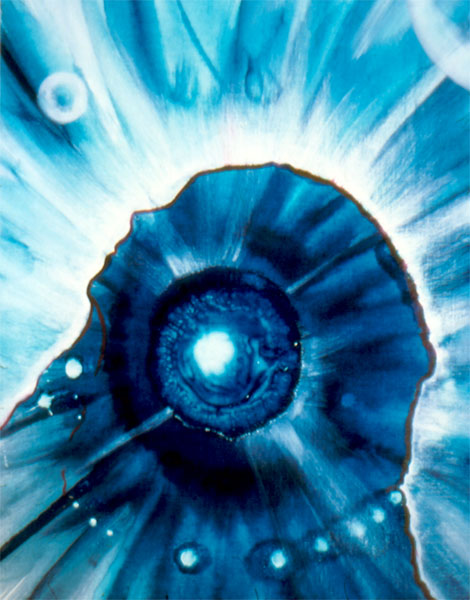
\includegraphics[width=0.82\columnwidth]{images/Morontia-Soul.jpg}\caption{Моронтийная душа, Винсент Вентола.}\end{figure}}
\vs p029 4:13 Личность не обязательно сопутствует разуму. Разум может мыслить даже если он полностью лишён способности выбора, как это наблюдается у многочисленных низших типов животных и у некоторых из этих подчинённых физических регуляторов. Многие из этих более автоматических регуляторов физической мощи не являются личностями ни в каком смысле этого слова. Они не наделены волей и способностью принимать независимые решения, будучи полностью подчинёнными механическому совершенству конструкции для задач, которые на них возложены. Тем не менее все они являются высокоразумными существами.
\vs p029 4:14 Физические регуляторы в основном заняты настройкой основных энергий, не открытых на Урантии. Эти неизвестные энергии очень важны для межпланетной системы транспорта и для некоторых способов связи. Когда мы прокладываем линии энергии с целью передачи эквивалентов звука или расширения зрения, эти неоткрытые формы энергии используются живыми физическими контролерами и их партнёрами. Эти же энергии иногда используются промежуточными созданиями в их повседневной работе\fnst{Действительно, при контактах с серафимами при поддержке промежуточных созданий происходит расширение зрения за пределы обычной октавы видимого света. В этой связи любопытно отметить следующий факт: при расширении зрения для восприятия формы серафима (например, в виде красного огненного столба) или формы моронтийной души (в виде голубого пульсирующего шара в области между горлом и солнечным сплетением, с нитями и <<клубами дыма>> внутри), все окружающие материальные предметы представляются \bibemph{чёрно\hyp{}белыми,} тогда как предметы из <<расширенной области>> видны в \bibemph{цвете}.}.\tunemarkup{pictures}{\begin{figure}[H]\centering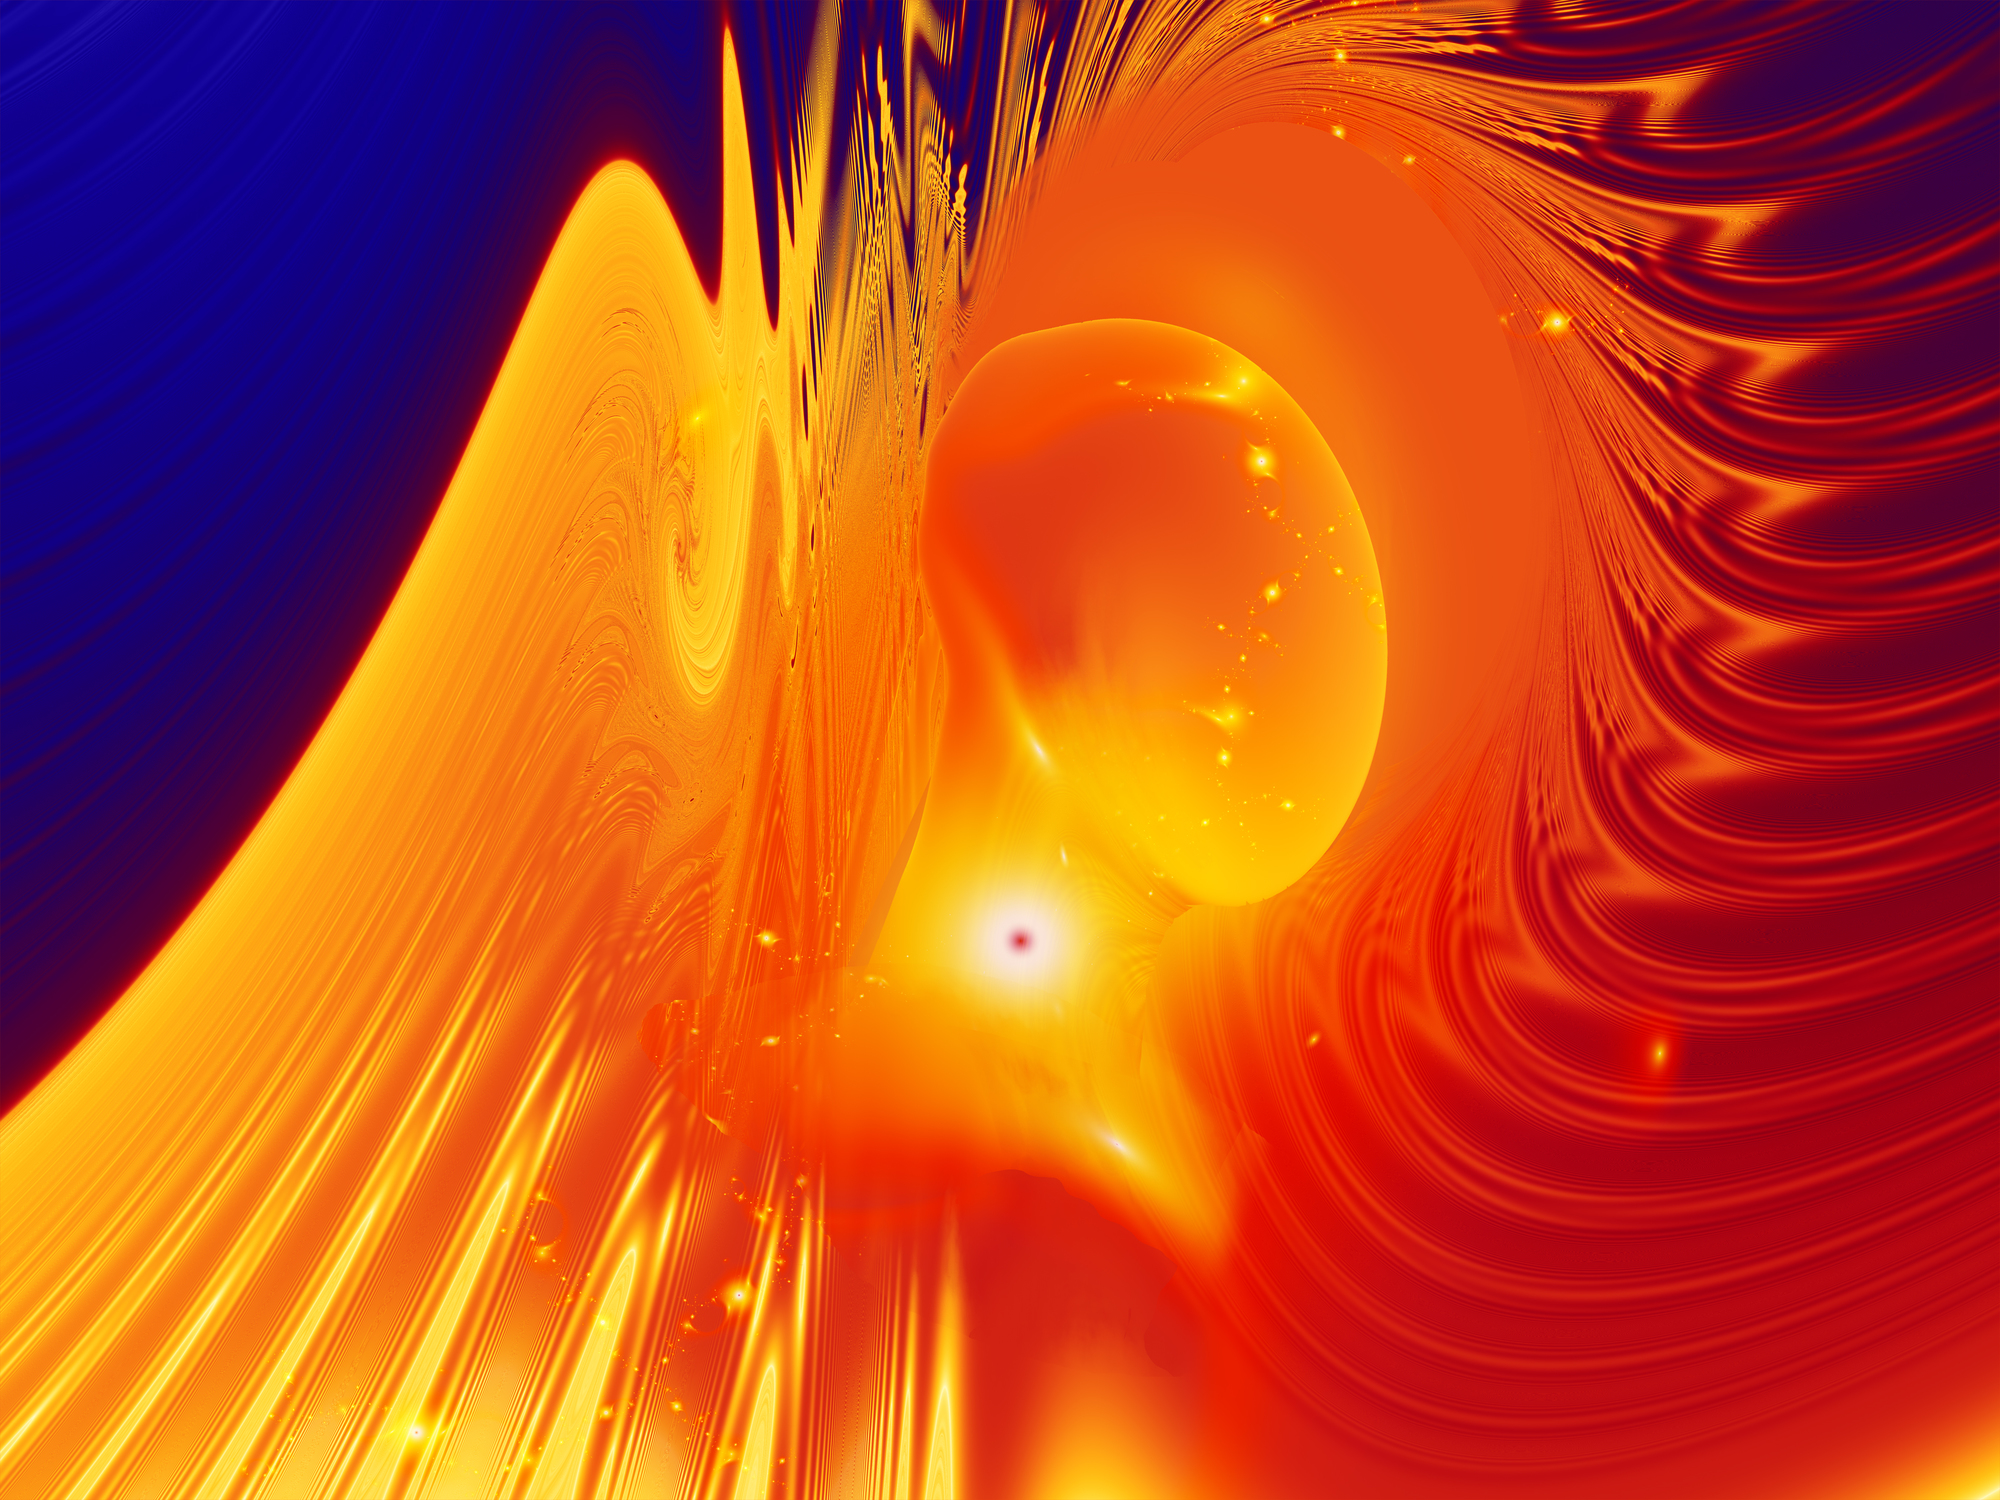
\includegraphics[width=0.95\columnwidth]{images/Seraphim.jpg}\caption{Серафим, Трой Бишоп.}\end{figure}}
\vs p029 4:15 \li{1.}\bibemph{Младшие Управляющие Мощью}. Этим удивительно эффективным существам доверено назначение и отправка всех категорий Главных Физических Регуляторов в соответствии с постоянно меняющимися потребностями постоянно изменяющегося энергетического статуса миров. Огромные резервы физических регуляторов поддерживаются на столичных мирах малых секторов, и из этих концентрационных пунктов они периодически отправляются младшими управляющими мощью в столицы вселенных, созвездий и систем, а также на отдельные планеты. Получив такое назначение, физические регуляторы временно подчиняются приказам божественных исполнителей миротворческих комиссий, но в остальном подчиняются исключительно своим помощникам управляющим и Верховным Центрам Мощи.
\vs p029 4:16 В каждый из малых секторов Орвонтона назначено 3\,000\,000 младших управляющих мощью, что в сумме составляет 3\,000\,000\,000 в качестве сверхвселенской квоты этих удивительно разносторонних существ. Их собственные резервы содержатся на тех же самых мирах малых секторов, где они служат также в качестве инструкторов для всех, кто изучает науки о методах интеллектуального контроля и трансмутации энергии.
\vs p029 4:17 Эти управляющие чередуют периоды исполнительной службы в малых секторах с равными периодами инспекционной службы в мирах пространства. Хотя бы один действующий инспектор всегда присутствует в каждой локальной системе, поддерживая центр на её столичной сфере. Они поддерживают гармоничную синхронизацию всего обширного скопления живой энергии.
\vs p029 4:18 \li{2.}\bibemph{Механические регуляторы}. Это чрезвычайно разносторонние и мобильные помощники младших управляющих мощью. Триллионы и триллионы их посылаются в Энсу, ваш малый сектор. Эти существа называются механическими регуляторами, потому что они полностью подвластны своим вышестоящим, целиком подчинены воле младших управляющих мощью. Тем не менее они сами по себе весьма умны, и их работа, хотя и механическая и прозаичная по природе своей, выполняется умело.
\vs p029 4:19 Из всех Главных Физических Регуляторов, назначенных в обитаемые миры, механические регуляторы безусловно являются самыми могущественными. Обладая живым даром антигравитации, больше всех других существ, каждый регулятор обладает сопротивлением гравитации, сравнимым только с сопротивлением гигантских сфер, вращающихся с огромной скоростью. Десять из этих регуляторов в настоящее время несут службу на Урантии, и одним из важнейших видов их планетарной деятельности является содействие отправлению серафических транспортов. При выполнении этой функции все 10 механических регуляторов действуют в унисон, в то время как батарея из 1\,000 передатчиков энергии обеспечивает начальный импульс для отправления серафима.
\vs p029 4:20 Механические регуляторы способны направлять поток энергии и способствовать её концентрации в специализированных токах или контурах. Эти могущественные существа непосредственно связаны с сегрегацией, направлением и усилением физических энергий и с уравновешиванием напряжений межпланетных контуров. Они являются экспертами в управлении 21 из 30 физических энергий пространства, составляющих энергетический заряд сверхвселенной. Им также удаётся добиться многого в управлении и контроле над 6 из 9 более тонких форм физической энергии. Помещая этих регуляторов в подходящем техническом отношении друг с другом и с определёнными центрами мощи, младшие управляющие мощью получают возможность производить невероятные изменения в настройке мощи и управлении энергией.
\vs p029 4:21 Главные Физические Регуляторы часто действуют в батареях из сотен, тысяч и даже миллионов, и, изменяя своё положение и построение, могут управлять энергией как коллективно, так и индивидуально. По мере изменения требований они могут повышать и ускорять объём и движение энергии или задерживать, конденсировать и замедлять энергетические токи. Они влияют на преобразования энергии и мощи подобно так называемым катализаторам, усиливающим химические реакции. Они функционируют благодаря врождённым способностям и в сотрудничестве с Верховными Центрами Мощи.
\vs p029 4:22 \li{3.}\bibemph{Преобразователи энергии}. Число этих существ в сверхвселенной невероятно велико. Только в одной Сатании их почти 1\,000\,000, а обычная квота составляет 100 на каждый обитаемый мир.
\vs p029 4:23 Преобразователи энергии являются совместным творением Семи Верховных Управляющих Мощью и Семи Управляющих Центрами\fnst{В тексте первого издания 1955 года <<Seven Central Supervisors>>, то есть <<Семь Центральных Управляющих>>, но текст был изменён на <<Seven Centre Supervisors>>, ибо последние известны из \bibref[29:2.10]{p029 2:10}, а первые нигде больше не упоминаются.}. Они относятся к числу более личностных категорий физических регуляторов, и за исключением тех случаев, когда на обитаемом мире присутствует младший управляющий мощью, руководство осуществляют преобразователи. Они являются планетарными инспекторами всех отбывающих серафических транспортов. Все классы небесной жизни могут использовать менее личностные категории физических регуляторов только посредством связи с более личностными категориями младших управляющих и преобразователей энергии.
\vs p029 4:24 Эти преобразователи представляют собой мощные и эффективные живые переключатели, будучи в состоянии располагаться по или против данного расположения или направления мощи. Они также искусно изолируют планеты от мощных потоков энергии, проходящих между гигантскими планетарными и звёздными соседями. Способность преобразовывать энергию делает их наиболее полезными в важной задаче поддержания всеобщего энергетического баланса или равновесия мощи. В какие\hyp{}то моменты кажется, что они потребляют или накапливают энергию; в другие,~--- что они источают или высвобождают энергию. Преобразователи способны увеличивать или уменьшать <<аккумуляторный>> потенциал живых и мёртвых энергий в соответствующих им областях. Но они имеют дело только с физическими и полуматериальными энергиями, они не функционируют непосредственно в сфере жизни, как не меняют они и формы живых существ.
\vs p029 4:25 В некоторых отношениях преобразователи энергии~--- самые удивительные и загадочные из всех полуматериальных живых созданий. Они каким\hyp{}то неизвестным образом физически отличаются, и, изменяя отношения своих связей, они могут оказывать глубокое влияние на энергию, которая проходит через их объединённые присутствия. Статус физических миров, по\hyp{}видимому, претерпевает трансформацию вследствие их искусных манипуляций. \bibemph{Они могут и действительно изменяют физическую форму энергий пространства}. С помощью своих партнёров\hyp{}регуляторов они фактически способны изменять форму и потенциал 27 из 30 физических энергий сверхвселенского заряда мощи. То, что три из этих энергий находятся вне их контроля, доказывает, что Безусловный Абсолют не действует посредством их.
\vs p029 4:26 \pc Остальные четыре группы Главных Физических Регуляторов вряд ли являются личностями в каком\hyp{}либо приемлемом определении этого слова. Эти передатчики, ассоциаторы, диссоциаторы и франдаланки полностью автоматичны в своих реакциях; тем не менее они разумны в полном смысле слова. Мы очень ограничены в наших знаниях об этих чудесных существах, потому что не можем общаться с ними. Они, кажется, понимают языки миров, но не могут общаться с нами. По\hyp{}видимому, они вполне способны принимать наши сообщения, но совершенно бессильны на них ответить.
\vs p029 4:27 \li{3.}\bibemph{Передатчики энергии}. Эти существа действуют главным образом, но не полностью, во внутрипланетном качестве. Они являются чудесными передатчиками энергии в той форме, в какой она проявляется на индивидуальных мирах.
\vs p029 4:28 Когда энергию нужно отвести в новый контур, передатчики выстраиваются в линию вдоль желаемого пути энергии, и в силу своих уникальных атрибутов притяжения энергии они могут действительно вызвать усиленный поток энергии в желаемом направлении. Они делают это так же буквально, как определённые металлические цепи направляют поток определённых форм электрической энергии; и они являются живыми сверхпроводниками для более чем половины из 30 форм физической энергии.
\vs p029 4:29 Передатчики искусно образуют связи, эффективно восстанавливающие слабеющие токи специализированной энергии, проходящие от планеты к планете и от станции к станции на отдельной планете. Они могут обнаруживать токи, которые слишком слабы для восприятия любым другим типом живого существа, и они могут так усиливать эти энергии, что сопровождающее их сообщение становится вполне разборчивым. Их услуги бесценны для приёмников трансляций.
\vs p029 4:30 Передатчики энергии могут работать со всеми формами передаваемого восприятия; они могут сделать удалённую сцену <<видимой>>, а далёкий звук <<слышимым>>. Они обеспечивают аварийные линии связи в локальных системах и на отдельных планетах. Эти услуги необходимы практически всем созданиям для связи за пределами регулярно установленных контуров.
\vs p029 4:31 Эти существа вместе с преобразователями энергии незаменимы для поддержания смертного существования на мирах с обеднённой атмосферой, и являются неотъемлемой частью жизненного процесса на планетах недышащих.
\vs p029 4:32 \li{5.}\bibemph{Первичные ассоциаторы}. Эти интересные и бесценные сущности являются непревзойдёнными накопителями и хранителями энергии. Подобно тому, как растение накапливает солнечный свет, так и эти живые организмы накапливают энергию во времена её избытка [plus manifestations]. Они работают в гигантском масштабе, преобразовывая энергии пространства в физическое состояние, неизвестное на Урантии. Они также способны продолжать эти преобразования вплоть до точки создания некоторых примитивных единиц материального существования. Эти существа просто действуют своим присутствием. Они никоим образом не истощаются и не опустошаются этой функцией; они действуют как живые катализаторы.
\vs p029 4:33 В периоды недостатка [minus manifestations] они имеют возможность высвобождать эти накопленные энергии. Но твоё знание об энергии и материи недостаточно развито, чтобы можно было объяснить метод этой фазы их работы. Они всегда трудятся в соответствии со всеобщим законом, оперируя и манипулируя атомами, электронами и ультиматонами так же, как вы маневрируете типографским набором, заставляя одни и те же алфавитные символы рассказывать совершенно разные истории.
\vs p029 4:34 Ассоциаторы~--- это первая группа жизни, которая появляется на формирующейся материальной сфере, и они могут функционировать при физических температурах, которые ты бы считал совершенно несовместимыми с существованием живых существ. Они представляют собой форму жизни, которая просто выходит за рамки человеческого воображения. Вместе со своими сотрудниками, диссоциаторами, они являются самыми рабски покорными из всех разумных созданий.
\vs p029 4:35 \li{6.}\bibemph{Вторичные диссоциаторы}. По сравнению с первичными ассоциаторами, эти существа с огромными антигравитационными способностями являются работниками обратного действия [reverse workers]. Никогда нет никакой опасности того, что специальные или модифицированные формы физической энергии на локальных мирах или в локальных системах иссякнут, ибо эти живые образования наделены уникальной способностью вырабатывать неограниченные запасы энергии. Они занимаются, главным образом, выработкой почти неизвестной на Урантии формы энергии, из формы материи, которая ещё менее известна. Они~--- поистине алхимики пространства и чудотворцы времени. Но творя все свои чудеса, они никогда не преступают мандатов Космической Верховности.
\vs p029 4:36 \li{7.}\bibemph{Франдаланки}. Эти существа~--- совместное творение всех трёх категорий существ, контролирующих энергию: первичных и вторичных организаторов силы и управляющих мощью. Франдаланки~--- самые многочисленные из всех Главных Физических Регуляторов; число действующих только в Сатании выходит за пределы твоей концепции числа. Они размещены на всех обитаемых мирах и всегда связаны с физическими регуляторами более высоких категорий. Они действуют взаимозаменяемо в центральной вселенной, сверхвселенных и в областях внешнего пространства.
\vs p029 4:37 Франдаланки создаются в 30 подразделениях, по одному для каждой формы основной вселенской силы, и они функционируют исключительно как живые и автоматические датчики присутствия, напряжения и скорости. Эти живые барометры занимаются исключительно автоматической и безошибочной регистрацией статуса всех форм силы\hyp{}энергии. Они являются для физической вселенной тем, чем обширный механизм отражательности является для вселенной разума. Франдаланки, которые регистрируют время в дополнение к количественному и качественному присутствию энергии, называются \bibemph{хронолдеками}.
\vs p029 4:38 Я признаю, что франдаланки разумны, но не могу классифицировать их иначе, как живые машины. Пожалуй, единственный способ помочь тебе понять эти живые механизмы,~--- это сравнить их с вашими собственными механическими приспособлениями, действующими с почти разумной надёжностью и точностью. Так что если ты хочешь представить себе этих существ, задействуй своё воображение до такой степени, чтобы признать, что в большой вселенной у нас действительно есть разумные и \bibemph{живые} механизмы (сущности), которые могут выполнять более запутанные задачи, требующие более колоссальных вычислений с ещё большей чувствительностью к точности и с предельной надёжностью.
\usection{ГЛАВНЫЕ ОРГАНИЗАТОРЫ СИЛЫ}
\vs p029 5:1 Организаторы силы проживают на Рае, но они действуют по всей главной вселенной, особенно в областях неорганизованного пространства. Эти необыкновенные существа не являются ни создателями, ни созданиями, и они составляют два основных подразделения службы:
\vs p029 5:2 \li{1.}Первичные Возникшие Главные Организаторы Силы.
\vs p029 5:3 \li{2.}Младшие Трансцендентальные Главные Организаторы Силы.
\vs p029 5:4 \pc Эти две могущественные категории манипуляторов изначальной силы работают исключительно под наблюдением Зодчих Главной Вселенной, и в настоящее время они не ведут широкой деятельности в границах большой вселенной.
\vs p029 5:5 \pc Первичные Главные Организаторы Силы~--- это манипуляторы изначальных или основных пространственных сил [space\hyp{}force] Безусловного Абсолюта; они являются создателями туманностей\fnst{То есть галактик.}. Они~--- живые инициаторы энергетических циклонов пространства, а также организаторы и направляющие этих гигантских проявлений на ранних стадиях. Эти организаторы силы трансмутируют \bibemph{изначальную силу} (предэнергию, не реагирующую на прямую Райскую гравитацию) в первичную, или \bibemph{могучую энергию}~--- энергию, переходящую из исключительного охвата Безусловного Абсолюта в гравитационный охват Острова Рай. Далее на смену им приходят младшие организаторы силы, которые продолжают процесс трансмутации энергии от первичной к вторичной, или \bibemph{гравитационно\hyp{}энергетической,} стадии.
\vs p029 5:6 По завершении планов создания локальной вселенной, о чём свидетельствует прибытие Сына Создателя, Младшие Главные Организаторы Силы уступают место категориям управляющих мощью, действующих в сверхвселенной астрономического подчинения. Но в отсутствие таких планов помощники организаторы сил продолжают бессрочно заботиться об этих материальных творениях~--- именно так, как они сейчас это делают во внешнем пространстве.
\vs p029 5:7 Главные Организаторы Силы выдерживают температуры и функционируют в физических условиях, которые были бы непереносимы даже для разносторонних центров мощи и физических регуляторов Орвонтона. Кроме них, из раскрытых категорий существ только Одинокие Посланники и Вдохновлённые Троичные Духи способны функционировать во владениях внешнего пространства.
\vsetoff
\vs p029 5:8 [При поддержке Всеобщего Цензора, уполномоченного От Века Древними на Уверсе.]
\quizlink

\upaper{30}{ЛИЧНОСТИ БОЛЬШОЙ ВСЕЛЕННОЙ}
\uminitoc{РАЙСКАЯ КЛАССИФИКАЦИЯ ЖИВЫХ СУЩЕСТВ}
\uminitoc{РЕЕСТР ЛИЧНОСТЕЙ УВЕРСЫ}
\uminitoc{ГОСТЯЩИЕ КОЛОНИИ}
\uminitoc{ВОСХОДЯЩИЕ СМЕРТНЫЕ}
\author{Могущественный Посланник}
\vs p030 0:1 Личности и не являющиеся личностями сущности, функционирующие в настоящее время на Рае и в большой вселенной, составляют почти безграничное количество живых существ. Даже количество основных категорий и типов поразило бы человеческое воображение, не говоря уже о бесчисленных подтипах и разновидностях. Тем не менее желательно дать представление о двух основных классификациях живых существ: вариант Райской классификации и сокращённую форму Реестра Личностей Уверсы.
\vs p030 0:2 Невозможно сформулировать исчерпывающую и полностью последовательную классификацию личностей большой вселенной, потому что не \bibemph{все} группы раскрыты. Потребовалось бы множество дополнительных документов, чтобы охватить дальнейшее откровение, необходимое для систематической классификации всех групп. Такое концептуальное расширение вряд ли было бы желательным, поскольку оно лишило бы мыслящих смертных следующего тысячелетия того стимула к творческим размышлениям, которые дают эти частично раскрытые концепции. Лучше, если у человека не будет чрезмерного откровения; это подавляет воображение.
\usection{РАЙСКАЯ КЛАССИФИКАЦИЯ ЖИВЫХ СУЩЕСТВ}
\vs p030 1:1 Живые существа классифицируются на Рае в соответствии с присущими им и достигнутыми отношениями с Райскими Божествами. Во время великих собраний центральной вселенной  и сверхвселенных присутствующие часто группируются в соответствии с происхождением: триединого происхождения или достигшие Троицы; дуального происхождения; и одиночного происхождения. Трудно объяснить Райскую классификацию живых существ смертному разуму, но мы уполномочены представить следующее:
\vs p030 1:2 \li{I.}\bibemph{СУЩЕСТВА ТРИЕДИНОГО ПРОИСХОЖДЕНИЯ}. Существа, созданные всеми тремя Райскими Божествами~--- либо как таковые, либо в качестве Троицы,~--- а также Тринитизованный Корпус, это обозначение относится ко всем группам тринитизованных существ, раскрытых и нераскрытых.
\vs p030 1:3 \li{А.}\bibemph{Верховные Духи}.
\vs p030 1:4 \li{1.}Семь Главных Духов.
\vs p030 1:5 \li{2.}Семь Верховных Исполнителей.
\vs p030 1:6 \li{3.}Семь категорий Отражательных Духов.
\vs p030 1:7 \li{Б.}\bibemph{Стационарные Сыны Троицы}.
\vs p030 1:8 \li{1.}Тринитизованные Секреты Верховности.
\vs p030 1:9 \li{2.}От Века Вечные.
\vs p030 1:10 \li{3.}От Века Древние.
\vs p030 1:11 \li{4.}От Века Совершенные.
\vs p030 1:12 \li{5.}От Века Недавние.
\vs p030 1:13 \li{6.}От Века Единые.
\vs p030 1:14 \li{7.}От Века Верные.
\vs p030 1:15 \li{8.}Совершенствователи Мудрости.
\vs p030 1:16 \li{9.}Божественные Советники.
\vs p030 1:17 \li{10.}Всеобщие Цензоры.
\vs p030 1:18 \li{В.}\bibemph{Существа Троичного происхождения и тринитизованные существа}.
\vs p030 1:19 \li{1.}Троичные Сыны Учителя.
\vs p030 1:20 \li{2.}Вдохновлённые Троичные Духи.
\vs p030 1:21 \li{3.}Уроженцы Хавоны.
\vs p030 1:22 \li{4.}Граждане Рая.
\vs p030 1:23 \li{5.}Нераскрытые существа Троичного происхождения.
\vs p030 1:24 \li{6.}Нераскрытые существа, тринитизованные Божествами.
\vs p030 1:25 \li{7.}Тринитизованные Сыны Достижения.
\vs p030 1:26 \li{8.}Тринитизованные Сыны Отбора.
\vs p030 1:27 \li{9.}Тринитизованные Сыны Совершенства.
\vs p030 1:28 \li{10.}Сыны, тринитизованные созданиями.
\vs p030 1:29 \li{II.}\bibemph{СУЩЕСТВА ДВОЙСТВЕННОГО ПРОИСХОЖДЕНИЯ}. Существа, происходящие от любых двух Райских Божеств или иным образом созданные любыми двумя существами прямого или косвенного происхождения от Райских Божеств.
\vs p030 1:30 \li{А.}\bibemph{Нисходящие категории}.
\vs p030 1:31 \li{1.}Сыны Создатели.
\vs p030 1:32 \li{2.}Сыны Повелители.
\vs p030 1:33 \li{3.}Яркие Утренние Звёзды.
\vs p030 1:34 \li{4.}Отцы Мелхиседеки.
\vs p030 1:35 \li{5.}Мелхиседеки.
\vs p030 1:36 \li{6.}Ворондадеки.
\vs p030 1:37 \li{7.}Ланонандеки.
\vs p030 1:38 \li{8.}Блистательные Вечерние Звёзды.
\vs p030 1:39 \li{9.}Архангелы.
\vs p030 1:40 \li{10.}Носители Жизни.
\vs p030 1:41 \li{11.}Нераскрытые Вселенские Помощники.
\vs p030 1:42 \li{12.}Нераскрытые Сыны Бога.
\vs p030 1:43 \li{Б.}\bibemph{Стационарные категории}.
\vs p030 1:44 \li{1.}Абандонтеры.
\vs p030 1:45 \li{2.}Сусации.
\vs p030 1:46 \li{3.}Унивитации.
\vs p030 1:47 \li{4.}Спиронги.
\vs p030 1:48 \li{5.}Нераскрытые существа двойственного происхождения.
\vs p030 1:49 \li{В.}\bibemph{Восходящие категории}.
\vs p030 1:50 \li{1.}Смертные, слившиеся с Настройщиком.
\vs p030 1:51 \li{2.}Смертные, слившиеся с Сыном.
\vs p030 1:52 \li{3.}Смертные, слившиеся с Духом.
\vs p030 1:53 \li{4.}Преображённые промежуточные создания.
\vs p030 1:54 \li{5.}Нераскрытые восходящие существа.
\vs p030 1:55 \li{III.}\bibemph{СУЩЕСТВА ОДИНОЧНОГО ПРОИСХОЖДЕНИЯ}.
\vs p030 1:56 \li{А.}\bibemph{Верховные Духи}.
\vs p030 1:57 \li{1.}Гравитационные Посланники.
\vs p030 1:58 \li{2.}Семь Духов Контуров Хавоны.
\vs p030 1:59 \li{3.}Двенадцатичастные Помощники Контуров Хавоны.
\vs p030 1:60 \li{4.}Помощники Отражательного Изображения.
\vs p030 1:61 \li{5.}Вселенские Материнские Духи.
\vs p030 1:62 \li{6.}Семичастные Адъютанты Разумо\hyp{}Духи.
\vs p030 1:63 \li{7.}Нераскрытые существа, происходящие от Божеств.
\vs p030 1:64 \li{Б.}\bibemph{Восходящие категории}.
\vs p030 1:65 \li{1.}Персонализированные Настройщики.
\vs p030 1:66 \li{2.}Восходящие Материальные сыны.
\vs p030 1:67 \li{3.}Эволюционные серафимы.
\vs p030 1:68 \li{4.}Эволюционные херувимы.
\vs p030 1:69 \li{5.}Нераскрытые восходящие создания.
\vs p030 1:70 \li{В.}\bibemph{Семейство Бесконечного Духа}.
\vs p030 1:71 \li{1.}Одинокие Посланники.
\vs p030 1:72 \li{2.}Смотрители Вселенских Контуров.
\vs p030 1:73 \li{3.}Управляющие Переписью.
\vs p030 1:74 \li{4.}Личные Помощники Бесконечного Духа.
\vs p030 1:75 \li{5.}Младшие Инспекторы.
\vs p030 1:76 \li{6.}Назначенные Стражи.
\vs p030 1:77 \li{7.}Проводники Выпускников.
\vs p030 1:78 \li{8.}Сервиталы Хавоны.
\vs p030 1:79 \li{9.}Всеобщие Миротворцы.
\vs p030 1:80 \li{10.}Моронтийные Спутники.
\vs p030 1:81 \li{11.}Супернафимы.
\vs p030 1:82 \li{12.}Секонафимы.
\vs p030 1:83 \li{13.}Терциафимы.
\vs p030 1:84 \li{14.}Омниафимы.
\vs p030 1:85 \li{15.}Серафимы.
\vs p030 1:86 \li{16.}Херувимы и сановимы.
\vs p030 1:87 \li{17.}Нераскрытые существа, происходящие от Духа.
\vs p030 1:88 \li{18.}Семь Верховных Управляющих Мощью.
\vs p030 1:89 \li{19.}Верховные Центры Мощи.
\vs p030 1:90 \li{20.}Главные Физические Регуляторы.
\vs p030 1:91 \li{21.}Управляющие Моронтийной Мощью.
\vs p030 1:92 \li{IV.}\bibemph{ВОЗНИКШИЕ ТРАНСЦЕНДЕНТАЛЬНЫЕ СУЩЕСТВА}. На Рае можно найти великое множество трансцендентальных существ, происхождение которых обычно не раскрывается вселенным времени и пространства, пока они не утверждаются в свете и жизни. Эти Трансценденталы не являются ни создателями, ни созданиями; они~--- \bibemph{возникшие} [\bibemph{eventuated}] дети божественности, предельности и вечности. Эти <<возникшие>> [``eventuators''] не являются ни конечными, ни бесконечными~--- они \bibemph{абсонитны;} а абсонитность~--- это ни бесконечность, ни абсолютность.
\vs p030 1:93 Эти несозданные несоздатели всегда верны Райской Троице и послушны Предельному. Они существуют на четырёх предельных уровнях личностной активности и функционируют на семи уровнях абсонитного в двенадцати больших подразделениях, состоящих из тысячи основных рабочих групп по семь классов в каждой. Эти возникшие существа включают в себя следующие категории:
\vs p030 1:94 \li{1.}Зодчие Главной Вселенной.
\vs p030 1:95 \li{2.}Трансцендентальные Писцы.
\vs p030 1:96 \li{3.}Прочие Трансценденталы.
\vs p030 1:97 \li{4.}Первичные Возникшие Главные Организаторы Силы.
\vs p030 1:98 \li{5.}Младшие Трансцендентальные Главные Организаторы Силы.
\vs p030 1:99 \pc Бог, как сверхличность, возникает; Бог, как личность, творит; Бог, как доличность, фрагментируется; и такой фрагмент его самого, как Настройщик, развивает душу духа на базе материального и смертного разума в соответствии с добровольным выбором личности, которая была дарована такому смертному созданию родительским актом Бога как Отца.
\vs p030 1:100 \li{V.}\bibemph{ФРАГМЕНТИРОВАННЫЕ СУЩНОСТИ БОЖЕСТВА}. Эта категория живого существования, происходящая от Всеобщего Отца, лучше всего представлена Настройщиками Мыслей, хотя эти сущности ни в коем случае не являются единственными фрагментами доличностной реальности Первого Источника и Центра. Функции фрагментов, не являющихся Настройщиками, многочисленны и мало известны. Слияние с Настройщиком или другим подобным фрагментом составляет \bibemph{существо, слившееся с Отцом}.
\vs p030 1:101 Здесь следует отметить фрагментации предр\'азумного духа Третьего Источника и Центра, хотя они едва ли сравнимы с фрагментами Отца. Такие сущности очень сильно отличаются от Настройщиков; как таковые, они не обитают на Духограде и не перемещаются по контурам гравитации разума; не вселяются они и в смертные создания в течение жизни во плоти. Они не являются доличностными в том смысле, в каком являются Настройщики, но такие фрагменты предр\'азумного духа даруются некоторым выжившим смертным, и слияние с ними делает их \bibemph{слившимися с Духом смертными,}~--- в отличие от смертных, слившихся с Настройщиком.
\vs p030 1:102 Ещё труднее описать индивидуализированный дух Сына Создателя, союз с которым делает создание \bibemph{смертным, слившимся с Сыном}. Существуют и другие фрагментации Божества.
\vs p030 1:103 \li{VI.}\bibemph{СВЕРХЛИЧНОСТНЫЕ СУЩЕСТВА}. Во вселенной вселенных существует великое воинство неличностных существ божественного происхождения и разнообразного служения. Некоторые из этих существ обитают на Райских мирах Сына; другие, как сверхличностные представители Вечного Сына, встречаются повсюду. Они по большей части не упоминаются в этих повествованиях, и было бы совершенно бесполезно пытаться описать их \bibemph{личностным} существам.
\vs p030 1:104 \li{VII.}\bibemph{НЕКЛАССИФИЦИРОВАННЫЕ И НЕРАСКРЫТЫЕ КАТЕГОРИИ}. В течение нынешней вселенской эпохи было бы невозможно уложить всех существ, личностных и иных, в рамки классификации, относящейся к нынешней вселенской эпохе; кроме того, не все такие категории раскрыты в этих повествованиях; поэтому многочисленные категории были опущены в этих списках. Обрати внимание на следующие:
\vs p030 1:105 Завершитель Вселенского Предназначения.
\vs p030 1:106 Условные Наместники Предельного.
\vs p030 1:107 Безусловные Смотрители Верховного.
\vs p030 1:108 Нераскрытые Созидательные Силы От Века Древних.
\vs p030 1:109 Мажестон Рая.
\vs p030 1:110 Неназванные Отражательные Связные Мажестона.
\vs p030 1:111 Мидсонитные категории локальных вселенных.
\vs p030 1:112 \pc Не нужно придавать особого значения перечислению этих категорий вместе, кроме того, что ни один из них не фигурирует в Райской классификации в том виде, в котором она здесь раскрыта. Это лишь немногие из не вошедших в классификацию; тебе ещё предстоит узнать о многих нераскрытых.
\vs p030 1:113 Существуют различные духи: духи\hyp{}сущности, духи\hyp{}присутствия, личностные духи, доличностные духи, сверхличностные духи, духи\hyp{}существования, духи\hyp{}личности~--- но здесь не адекватны\fnst{То, что язык и интеллект смертных не адекватны очевидно хотя бы из того, что совершенно неясно, почему <<личностные духи>> и <<духи\hyp{}личности>> упомянуты отдельно.} ни язык смертных, ни смертный интеллект. Тем не менее мы можем отметить, что не существует личностей <<чистого разума>>; ни одна сущность не обладает личностью, если она не была наделена ею Богом, который есть дух. Любая разумная сущность, не связанная ни с духовной, ни с физической энергией, не является личностью. Но в том же смысле, в каком существуют духи\hyp{}личности, которые имеют разум, существуют разумы\hyp{}личности, которые имеют дух. Мажестон и его партнёры являются довольно хорошими иллюстрациями существ, у которых разум доминирует, но есть и лучшие иллюстрации этого типа личности, которые вам неизвестны. Существуют даже целые нераскрытые категории таких \bibemph{личностей разума,} но они всегда связаны с духом. Некоторые другие нераскрытые создания можно было бы назвать \bibemph{личностями разумо\hyp{}энергетическими и физико\hyp{}энергетическими}. Этот тип существ невосприимчив к гравитации духа, но тем не менее является истинной личностью~--- находится в контуре Отца.
\vs p030 1:114 \pc Эти документы не могут даже начать исчерпывающее изложение рассказа о живых существах, создателях, возникших и существующих иным образом существ, которые живут, поклоняются и служат в кишащих созданиями вселенных времени и в центральной вселенной вечности. Вы, смертные, являетесь личностями; поэтому мы можем описывать существа, которые \bibemph{персонализированы,} но как можно объяснить вам \bibemph{абсонитизированное} существо?
\usection{РЕЕСТР ЛИЧНОСТЕЙ УВЕРСЫ}
\vs p030 2:1 Божественная семья живых существ зарегистрирована на Уверсе в семи основных разделах:
\vs p030 2:2 \li{1.}Райские Божества.
\vs p030 2:3 \li{2.}Верховные Духи.
\vs p030 2:4 \li{3.}Существа Троичного происхождения.
\vs p030 2:5 \li{4.}Сыны Бога.
\vs p030 2:6 \li{5.}Личности Бесконечного Духа.
\vs p030 2:7 \li{6.}Управляющие Вселенской Мощью.
\vs p030 2:8 \li{7.}Корпус Постоянного Гражданства.
\vs p030 2:9 \pc Эти группы волевых существ делятся на многочисленные классы и малые подразделения. Однако изложение данной классификации личностей большой вселенной главным образом связано с представлением тех категорий разумных существ, которые были раскрыты в этих повествованиях, большинство из которых будут встречаться в опыте восхождения смертных времени на их постепенном подъёме к Раю. В нижеследующих списках не упоминаются обширные категории вселенских существ, которые выполняют свою работу вне плана восхождения смертных.
\vs p030 2:10 \li{I.}\bibemph{РАЙСКИЕ БОЖЕСТВА}.
\vs p030 2:11 \li{1.}Всеобщий Отец.
\vs p030 2:12 \li{2.}Вечный Сын.
\vs p030 2:13 \li{3.}Бесконечный Дух.
\vs p030 2:14 \li{II.}\bibemph{ВЕРХОВНЫЕ ДУХИ}.
\vs p030 2:15 \li{1.}Семь Главных Духов.
\vs p030 2:16 \li{2.}Семь Верховных Исполнителей.
\vs p030 2:17 \li{3.}Семь групп Отражательных Духов.
\vs p030 2:18 \li{4.}Помощники Отражательного Изображения.
\vs p030 2:19 \li{5.}Семь Духов Контуров.
\vs p030 2:20 \li{6.}Созидательные Духи локальных вселенных.
\vs p030 2:21 \li{7.}Адъютанты Разумо\hyp{}Духи.
\vs p030 2:22 \tunemarkup{pgnexus10}{\kern-4pt}\li{III.}\tunemarkup{pgnexus10}{\kern-5pt}\bibemph{СУЩЕСТВА ТРОИЧНОГО ПРОИСХОЖДЕНИЯ}.
\vs p030 2:23 \li{1.}Тринитизованные Секреты Верховности.
\vs p030 2:24 \li{2.}От Века Вечные.
\vs p030 2:25 \li{3.}От Века Древние.
\vs p030 2:26 \li{4.}От Века Совершенные.
\vs p030 2:27 \li{5.}От Века Недавние.
\vs p030 2:28 \li{6.}От Века Единые.
\vs p030 2:29 \li{7.}От Века Верные.
\vs p030 2:30 \li{8.}Троичные Сыны Учителя.
\vs p030 2:31 \li{9.}Совершенствователи Мудрости.
\vs p030 2:32 \li{10.}Божественные Советники.
\vs p030 2:33 \li{11.}Вселенские Цензоры.
\vs p030 2:34 \li{12.}Вдохновлённые Троичные Духи.
\vs p030 2:35 \li{13.}Уроженцы Хавоны.
\vs p030 2:36 \li{14.}Граждане Рая.
\vs p030 2:37 \li{IV.}\bibemph{СЫНЫ БОГА}.
\vs p030 2:38 \li{A.}\bibemph{Нисходящие Сыны}.
\vs p030 2:39 \li{1.}Сыны Создатели~--- Михаилы.
\vs p030 2:40 \li{2.}Сыны Повелители~--- Авоналы.
\vs p030 2:41 \li{3.}Троичные Сыны Учителя~--- Дайналы.
\vs p030 2:42 \li{4.}Сыны Мелхиседеки.
\vs p030 2:43 \li{5.}Сыны Ворондадеки.
\vs p030 2:44 \li{6.}Сыны Ланонандеки.
\vs p030 2:45 \li{7.}Сыны Носители Жизни.
\vs p030 2:46 \li{Б.}\bibemph{Восходящие Сыны}.
\vs p030 2:47 \li{1.}Слившиеся с Отцом смертные.
\vs p030 2:48 \li{2.}Слившиеся с Сыном смертные.
\vs p030 2:49 \li{3.}Слившиеся с Духом смертные.
\vs p030 2:50 \li{4.}Эволюционные серафимы.
\vs p030 2:51 \li{5.}Восходящие Материальные Сыны.
\vs p030 2:52 \li{6.}Преображённые промежуточные создания.
\vs p030 2:53 \li{7.}Персонализированные Настройщики.
\vs p030 2:54 \li{В.}\bibemph{Тринитизованные Сыны}.
\vs p030 2:55 \li{1.}Могущественные Посланники.
\vs p030 2:56 \li{2.}Высокоуполномоченные.
\vs p030 2:57 \li{3.}Не Имеющие Имени и Номера.
\vs p030 2:58 \li{4.}Тринитизованные Хранители.
\vs p030 2:59 \li{5.}Тринитизованные Послы.
\vs p030 2:60 \li{6.}Небесные Стражи.
\vs p030 2:61 \li{7.}Помощники Высоких Сынов.
\vs p030 2:62 \li{8.}Сыны, тринитизованные восходящими созданиями.
\vs p030 2:63 \li{9.}Тринитизованные Сыны Рая Хавоны.
\vs p030 2:64 \li{10.}Тринитизованные Сыны Предназначения.
\vs p030 2:65 \li{V.}\bibemph{ЛИЧНОСТИ БЕСКОНЕЧНОГО ДУХА}.
\vs p030 2:66 \li{А.}\bibemph{Высшие Личности Бесконечного Духа}.
\vs p030 2:67 \li{1.}Одинокие Посланники.
\vs p030 2:68 \li{2.}Смотрители Вселенских Контуров.
\vs p030 2:69 \li{3.}Управляющие Переписью.
\vs p030 2:70 \li{4.}Личные Помощники Бесконечного Духа.
\vs p030 2:71 \li{5.}Младшие Инспекторы.
\vs p030 2:72 \li{6.}Назначенные Стражи.
\vs p030 2:73 \li{7.}Проводники Выпускников.
\vs p030 2:74 \li{Б.}\bibemph{Воинства Посланников Пространства}.
\vs p030 2:75 \li{1.}Сервиталы Хавоны.
\vs p030 2:76 \li{2.}Всеобщие Миротворцы.
\vs p030 2:77 \li{3.}Технические Консультанты.
\vs p030 2:78 \li{4.}Хранители Райских Записей.
\vs p030 2:79 \li{5.}Небесные Писцы.
\vs p030 2:80 \li{6.}Моронтийные Спутники.
\vs p030 2:81 \li{7.}Райские Спутники.
\vs p030 2:82 \li{В.}\bibemph{Духи\hyp{}Помощники}.
\vs p030 2:83 \li{1.}Супернафимы.
\vs p030 2:84 \li{2.}Секонафимы.
\vs p030 2:85 \li{3.}Терциафимы.
\vs p030 2:86 \li{4.}Омниафимы.
\vs p030 2:87 \li{5.}Серафимы.
\vs p030 2:88 \li{6.}Херувимы и сановимы.
\vs p030 2:89 \li{7.}Промежуточные создания.
\vs p030 2:90 \li{VI.}\bibemph{УПРАВЛЯЮЩИЕ ВСЕЛЕНСКОЙ МОЩЬЮ}.
\vs p030 2:91 \li{А.}\bibemph{Семь Верховных Управляющих Мощью}.
\vs p030 2:92 \li{Б.}\bibemph{Верховные Центры Мощи}.
\vs p030 2:93 \li{1.}Верховные Управляющие Центрами.
\vs p030 2:94 \li{2.}Центры Хавоны.
\vs p030 2:95 \li{3.}Центры сверхвселенных.
\vs p030 2:96 \li{4.}Центры локальных вселенных.
\vs p030 2:97 \li{5.}Центры созвездий.
\vs p030 2:98 \li{6.}Центры систем.
\vs p030 2:99 \li{7.}Неклассифицированные Центры.
\vs p030 2:100 \li{В.}\bibemph{Главные Физические Регуляторы}.
\vs p030 2:101 \li{1.}Младшие Управляющие Мощью.
\vs p030 2:102 \li{2.}Механические регуляторы.
\vs p030 2:103 \li{3.}Преобразователи энергии.
\vs p030 2:104 \li{4.}Передатчики энергии.
\vs p030 2:105 \li{5.}Первичные ассоциаторы.
\vs p030 2:106 \li{6.}Вторичные диссоциаторы.
\vs p030 2:107 \li{7.}Франдаланки и хронолдеки.
\vs p030 2:108 \li{Г.}\bibemph{Управляющие Моронтийной Мощью}.
\vs p030 2:109 \li{1.}Регуляторы контуров.
\vs p030 2:110 \li{2.}Координаторы систем.
\vs p030 2:111 \li{3.}Планетарные Хранители.
\vs p030 2:112 \li{4.}Объединённые регуляторы.
\vs p030 2:113 \li{5.}Стабилизаторы связи.
\vs p030 2:114 \li{6.}Селективные сортировщики.
\vs p030 2:115 \li{7.}Младшие Регистраторы.
\vs p030 2:116 \tunemarkup{pgnexus10}{\kern4pt}\li{VII.}\bibemph{КОРПУС ПОСТОЯННОГО ГРАЖДАНСТВА}.
\vs p030 2:117 \li{1.}Планетарные промежуточные создания.
\vs p030 2:118 \li{2.}Адамические Сыны систем.
\vs p030 2:119 \li{3.}Унивитации созвездий.
\vs p030 2:120 \li{4.}Сусации локальных вселенных.
\vs p030 2:121 \li{5.}Слившиеся с Духом смертные локальных вселенных.
\vs p030 2:122 \li{6.}Абандонтеры сверхвселенных.
\vs p030 2:123 \li{7.}Слившиеся с Сыном смертные сверхвселенных.
\vs p030 2:124 \li{8.}Уроженцы Хавоны.
\vs p030 2:125 \li{9.}Уроженцы Райских сфер Духа.
\vs p030 2:126 \li{10.}Уроженцы Райских сфер Отца.
\vs p030 2:127 \li{11.}Сотворённые Граждане Рая.
\vs p030 2:128 \li{12.}Слившиеся с Настройщиком смертные Граждане Рая.
\vs p030 2:129 \pc Такова рабочая классификация личностей вселенных в том виде, как они зарегистрированы на столичном мире~--- на Уверсе.
\vs p030 2:130 \pc \bibemph{СМЕШАННЫЕ ГРУППЫ ЛИЧНОСТЕЙ}. На Уверсе существуют записи о многочисленных дополнительных группах разумных существ, существ, которые также тесно связаны с организацией и управлением большой вселенной. В число таких категорий входят следующие три смешанные группы личностей:
\vs p030 2:131 \li{А.}\bibemph{Райские Корпусы Завершения}.
\vs p030 2:132 \li{1.}Корпус Смертных Завершителей.
\vs p030 2:133 \li{2.}Корпус Райских Завершителей.
\vs p030 2:134 \li{3.}Корпус Тринитизованных Завершителей.
\vs p030 2:135 \li{4.}Корпус Совместных Тринитизованных Завершителей.
\vs p030 2:136 \li{5.}Корпус Завершителей Хавоны.
\vs p030 2:137 \li{6.}Корпус Трансцендентальных Завершителей.
\vs p030 2:138 \li{7.}Корпус Нераскрытых Сынов Предназначения.
\vs p030 2:139 \pc Смертный Корпус Завершения рассматривается в следующем и заключительном документе этой серии.
\vs p030 2:140 \li{Б.}\bibemph{Вселенские Помощники}.
\vs p030 2:141 \li{1.}Яркие Утренние Звёзды.
\vs p030 2:142 \li{2.}Блистательные Вечерние Звёзды.
\vs p030 2:143 \li{3.}Архангелы.
\vs p030 2:144 \li{4.}Всевышние Помощники.
\vs p030 2:145 \li{5.}Высокие Комиссары.
\vs p030 2:146 \li{6.}Небесные Наблюдатели.
\vs p030 2:147 \li{7.}Учителя Обительских Миров.
\vs p030 2:148 \pc На всех столичных мирах как локальных вселенных, так и сверхвселенных обеспечены условия для этих существ, выполняющих конкретные миссии для Сынов Создателей, правителей локальной вселенной. Мы радушно принимаем этих \bibemph{Вселенских Помощников} на Уверсе, но они не входят в нашу юрисдикцию. Эти эмиссары выполняют свою работу и проводят свои наблюдения под руководством Сынов Создателей. Их деятельность более полно описана в рассказе о вашей локальной вселенной.
\vs p030 2:149 \li{В.}\bibemph{Семь гостящих колоний}.
\vs p030 2:150 \li{1.}Исследователи звёзд.
\vs p030 2:151 \li{2.}Небесные мастеровые.
\vs p030 2:152 \li{3.}Управляющие реверсией.
\vs p030 2:153 \li{4.}Преподаватели подготовительных школ.
\vs p030 2:154 \li{5.}Различные резервные корпусы.
\vs p030 2:155 \li{6.}Приезжие студенты.
\vs p030 2:156 \li{7.}Восходящие пилигримы.
\vs p030 2:157 \pc Такова организация и управление этих семи групп существ на всех столичных мирах~--- от локальных систем до столиц сверхвселенных, особенно последних. Столицы семи сверхвселенных~--- это места встреч почти всех классов и категорий разумных существ. За исключением многочисленных групп жителей Рая\hyp{}Хавоны, здесь можно наблюдать и изучать волевые создания любой фазы существования.
\usection{ГОСТЯЩИЕ КОЛОНИИ}
\vs p030 3:1 Семь гостящих колоний временно проживают на архитектурных сферах в течение более или менее продолжительного времени, занятые осуществлением своих миссий и исполнением своих особых заданий. Их работа может быть описана следующим образом:
\vs p030 3:2 \li{1.}\bibemph{Исследователи звёзд}~--- небесные астрономы~--- предпочитают работать на сферах, подобных Уверсе, потому что такие специально сконструированные миры особенно благоприятны для их наблюдений и расчётов. Уверса удачно расположена для работы этой колонии не только из\hyp{}за её центрального местонахождения, но и потому, что поблизости нет гигантских живых или мёртвых солнц, которые приводили бы к возмущениям токов энергии. Эти исследователи никоим образом не связаны органично с делами сверхвселенной; они просто гости.
\vs p030 3:3 Астрономическая колония Уверсы включает индивидуумов из многих близлежащих миров, из центральной вселенной и даже из Норлатиадека. Любое существо из любого мира любой системы любой вселенной может стать исследователем звёзд, может стремиться вступить в один из корпусов небесных астрономов. Единственные необходимые условия: продолжение жизни и достаточное знание миров пространства, особенно их физических законов эволюции и контроля. Исследователи звёзд не обязаны служить в этом корпусе вечно, но никто, принятый в эту группу, не может уйти раньше одного тысячелетия по времени  Уверсы.
\vs p030 3:4 Колония звёздных наблюдателей Уверсы сейчас насчитывает более миллиона существ. Эти астрономы приходят и уходят, хотя некоторые остаются на сравнительно долгое время. Они выполняют свою работу с помощью множества механических инструментов и физических приспособлений; им также очень помогают Одинокие Посланники и другие духи\hyp{}исследователи. Эти небесные астрономы постоянно используют живых преобразователей и передатчиков энергии, а также отражательных личностей в своей работе по изучению звёзд и обследованию пространства. Они изучают все формы и фазы пространственных материальных и энергетических проявлений, и их так же сильно интересуют силовые функции, как и звёздные явления; ничто во всём пространстве не ускользает от их пристального внимания.
\vs p030 3:5 Подобные колонии астрономов можно встретить на столичных мирах секторов сверхвселенной, а также на архитектурных столицах локальных вселенных и их административных подразделениях. За исключением Рая, знание не является врождённым; понимание физической вселенной во многом зависит от наблюдений и исследований.
\vs p030 3:6 \li{2.}\bibemph{Небесные мастеровые} служат по всем семи сверхвселенным. Восходящие смертные впервые вступают в контакт с этими группами на моронтийном пути локальной вселенной, в связи с которой эти мастеровые и будут обсуждаться более подробно.
\vs p030 3:7 \li{3.}\bibemph{Управляющие реверсией} содействуют отдыху и поднятию настроения~--- возвращению к воспоминаниям о прошлом. Они очень полезны в практическом осуществлении плана восхождения смертных, особенно на ранних этапах моронтийного перехода и опыта духа. Рассказ о них относится к повествованию о пути смертных в локальной вселенной.
\vs p030 3:8 \li{4.}\bibemph{Преподаватели подготовительных школ}. Более высокий, следующий на пути восхождения мир обитания всегда поддерживает мощный корпус учителей в более низком, непосредственно предшествующем ему~--- своего рода подготовительную школу для развивающихся жителей этой сферы; это этап схемы восхождения для продвижения пилигримов времени. Эти школы, их методы обучения и проведения экзаменов совершенно не похожи на всё, что вы пытаетесь провести на Урантии.
\vs p030 3:9 Весь план восхождения по пути развития смертных характеризуется практикой передачи другим существам новой истины и опыта сразу же после их приобретения. Вы прокладываете себе путь через долгую школу Райского достижения, служа учителями ученикам, которые находятся сразу же за вами по уровню развития.
\vs p030 3:10 \li{5.}\bibemph{Различные резервные корпусы}. Огромные резервы существ, не находящихся под нашим непосредственным руководством, мобилизованы на Уверсе в качестве колонии резервных корпусов. На Уверсе действует 70 первичных подразделений этой колонии, и для получения разностороннего образования разрешается провести некоторое время с этими необыкновенными личностями. Подобные общие резервы поддерживаются на Спасограде и других вселенских столицах; они направляются на активную службу по запросу директоров соответствующих групп.
\vs p030 3:11 \li{6.}\bibemph{Приезжие студенты}. Со всей вселенной через различные столичные миры течёт непрерывный поток небесных посетителей. Индивидуально и в классах эти различные типы существ стекаются к нам в качестве наблюдателей, учеников по обмену и помощников исследователей. На Уверсе в настоящее время в этой гостевой колонии проживает более миллиарда лиц. Некоторые из этих посетителей могут задержаться на день, другие~--- на год, всё зависит от характера их миссии. В этой колонии обитают почти все классы вселенских существ, кроме личностей Создателей и моронтийных смертных.
\vs p030 3:12 Моронтийные смертные могут быть приезжими студентами только в пределах локальной вселенной своего происхождения. Они могут гостить в сверхвселенском качестве только после того, как достигнут статуса духа. Более половины посетителей в нашей колонии составляют <<транзитные>>~--- существа, путешествующие куда\hyp{}то в другое место, которые делают остановку, чтобы посетить столицу Орвонтона. Эти личности могут выполнять вселенское задание или наслаждаться периодом досуга~--- свободы от задания. Привилегия путешествий и наблюдений внутривселенского уровня~--- это часть пути всех восходящих существ. Человеческое желание путешествовать и наблюдать за новыми народами и мирами будет полностью удовлетворено во время долгого и насыщенного событиями восхождения в Рай через локальную, сверх\hyp{} и центральную вселенные.
\vs p030 3:13 \li{7.}\bibemph{Восходящие пилигримы}. Когда восходящие пилигримы назначаются на различные службы в связи с их Райским восхождением, они размещаются в качестве гостевой колонии на различных столичных сферах. Действуя повсюду в сверхвселенной, такие группы в основном самоуправляющиеся. Они представляют собой постоянно изменяющуюся колонию, охватывающую все категории эволюционных смертных и их товарищей по восхождению.
\usection{ВОСХОДЯЩИЕ СМЕРТНЫЕ}
\vs p030 4:1 Хотя выжившие смертные времени и пространства, принятые к постепенному восхождению к Раю, называются \bibemph{восходящими пилигримами,} эти эволюционные создания занимают такое важное место в данных повествованиях, что мы желаем дать здесь краткий обзор следующих семи стадий вселенского пути восхождения:
\vs p030 4:2 \li{1.}Планетарные смертные.
\vs p030 4:3 \li{2.}Выжившие спящие.
\vs p030 4:4 \li{3.}Студенты обительских миров.
\vs p030 4:5 \li{4.}Моронтийные прогрессоры.
\vs p030 4:6 \li{5.}Подопечные сверхвселенных.
\vs p030 4:7 \li{6.}Пилигримы Хавоны.
\vs p030 4:8 \li{7.}Прибывшие в Рай.
\vs p030 4:9 \pc В следующем повествовании представлен вселенский путь смертного, в котором обитает Настройщик. Слившиеся с Сыном или Духом смертные разделяют часть этого пути, но мы решили рассказать эту историю в той форме, в какой она относится к слившимся с Настройщиком смертным, поскольку такое предназначение могут ожидать все человеческие расы Урантии.
\vs p030 4:10 \li{1.}\bibemph{Планетарные смертные}. Все смертные~--- эволюционные существа животного происхождения с потенциалом восхождения. По происхождению, природе и предназначению эти различные группы и типы человеческих существ не слишком отличаются от народов Урантии. Человеческие расы каждого мира пользуются одинаковым служением Сынов Бога и присутствием духов\hyp{}помощников времени. После естественной смерти все типы восходящих созданий объединяются в одну моронтийную семью на обительских мирах.
\vs p030 4:11 \li{2.}\bibemph{Выжившие спящие}. Все смертные со статусом выживания, находящиеся под опекой личных хранителей предназначения, проходят через врата естественной смерти и, на третий период, персонализируются на обительских мирах. Те допущенные существа, которые по какой\hyp{}либо причине не смогли достичь того уровня владения разумом и наделения духовностью, который давал бы им право на личных хранителей, не могут таким образом немедленно и непосредственно отправиться в обительские миры. Такие выжившие души должны отдыхать в бессознательном сне до судного дня новой эпохи, новой диспенсации, прихода Сына Бога, чтобы сделать эпохальную перекличку и судить мир, и это общая практика по всему Небадону. О Христе Михаиле было сказано, что, когда он взошёл на небеса по завершении своей земной работы, <<Он увёл великое множество пленников>>. И эти пленники были спящими выжившими со времён Адама до дня воскресения Учителя на Урантии.
\vs p030 4:12 Течение времени не имеет значения для спящих смертных; они совершенно не осозна\'ют и не помнят продолжительности своего покоя. После реконструкции личности в конце эпохи те, кто проспал пять тысяч лет, будут реагировать не иначе, чем те, кто отдыхал пять дней. За исключением этой временн\'ой задержки, эти выжившие проходят режим восхождения так же, как и те, кто избежал более или менее продолжительного сна смерти.
\vs p030 4:13 Эти диспенсационные классы пилигримов миров используются для групповой моронтийной деятельности в работе локальных вселенных. Мобилизация таких огромных групп даёт большое преимущество; таким образом, они остаются вместе на долгие периоды эффективного служения.
\vs p030 4:14 \li{3.}\bibemph{Студенты обительских миров}. Все выжившие смертные, пробуждающиеся на обительских мирах, принадлежат к этому классу.
\vs p030 4:15 Физическое тело смертной плоти не является частью процесса реконструкции [reassembly] спящего выжившего; физическое тело возвратилось в прах. Назначенный серафим подготавливает [sponsors] новое тело, моронтийную форму, как новое жизненное средство\fnst{То есть новое средство самовыражения для той же самой личности.} для бессмертной души и для обитания вернувшегося Настройщика. Настройщик является хранителем духовной копии разума спящего выжившего. Назначенный серафим является хранителем сохранившейся индивидуальности~--- бессмертной души~--- в той мере, в какой она сформировалась. И когда эти двое~--- Настройщик и серафим~--- воссоединяют доверенные им собственности личности, новый индивидуум представляет собой воскрешение старой личности, выживание развивающейся моронтийной индивидуальности души. Такое воссоединение души и Настройщика вполне правильно называть воскресением, реконструкцией личностных факторов; но даже это не полностью объясняет повторное появление уцелевшей \bibemph{личности}. Хотя ты, вероятно, никогда не поймёшь факта такого необъяснимого процесса, ты когда\hyp{}нибудь эмпирически познаешь его истинность, если только не откажешься от плана выживания смертных.
\vs p030 4:16 \pc План первоначального содержания смертного под арестом на семи мирах постепенной подготовки действует почти универсально в Орвонтоне. В каждой локальной системе, состоящей примерно из тысячи обитаемых планет, есть семь обительских миров, обычно спутников или вторичных спутников\fnst{Спутников спутников.} столицы системы. Они являются принимающими мирами для большинства восходящих смертных.
\vs p030 4:17 Иногда все учебные миры, где обитают смертные, называют вселенскими <<обителями>>, и именно такие сферы имел в виду Иисус, когда сказал: <<В доме моего Отца много обителей>>. Отсюда и далее, в пределах одной группы сфер, таких как обительские миры, восходящие создания будут индивидуально продвигаться от одной сферы к другой и от одной фазы жизни к другой, но от одной ступени изучения вселенной к другой они всегда будут переходить классами.
\vs p030 4:18 \li{4.}\bibemph{Моронтийные прогрессоры}. Начиная с обительских миров и далее~--- через сферы системы, созвездия и вселенной,~--- смертные причисляются к классу моронтийных прогрессоров; они проходят переходные сферы восхождения смертных. Поднимаясь от низших моронтийных миров к высшим, восходящие смертные выполняют бесчисленные задания вместе со своими учителями и в компании своих дальше продвинувшихся и старших братьев.
\vs p030 4:19 Моронтийное развитие относится к непрерывному развитию интеллекта, духа и формы личности. Выжившие по\hyp{}прежнему остаются существами троякой природы. На протяжении всего моронтийного опыта они являются подопечными локальной вселенной. Режим сверхвселенной не действует до тех пор, пока не начнётся путь духа.
\vs p030 4:20 Смертные обретают настоящую индивидуальность духа непосредственно перед тем, как покинуть столицу локальной вселенной и отправиться в принимающие миры малых секторов сверхвселенной. Переход от заключительной моронтийной стадии к первому или низшему статусу духа представляет собой лишь небольшое изменение. Разум, личность и характер не меняются в результате такого продвижения; изменяется только форма. Но форма духа так же реальна, как и моронтийное тело, и не менее различима.
\vs p030 4:21 Прежде чем покинуть свои родные локальные вселенные и отправиться в принимающие миры сверхвселенной, смертные времени получают подтверждение духа от Сына Создателя и Материнского Духа локальной вселенной. С этого момента статус восходящего смертного утверждён навсегда. Никогда ещё подопечные сверхвселенной не сбивались с пути. Восходящие серафимы также продвигаются в ангельском статусе во время своего ухода из локальных вселенных.
\vs p030 4:22 \li{5.}\bibemph{Подопечные сверхвселенных}. Все восходящие существа, прибывающие на подготовительные миры сверхвселенных, становятся подопечными От Века Древних; они прошли моронтийную жизнь локальной вселенной и теперь стали признанными духами. Как молодые духи, они начинают восхождение в системе обучения и культуры сверхвселенной, начиная от принимающих сфер своего малого сектора через учебные миры десяти больших секторов и далее к высшим культурным сферам столицы сверхвселенной.
\vs p030 4:23 Существуют три категории духов\hyp{}учащихся, проживающих, соответственно, на столичных мирах развития духа малого сектора, больших секторов и сверхвселенной. Как восходящие моронтийные существа учились и работали на мирах локальной вселенной, так и восходящие духи продолжают осваивать новые миры, практикуясь в передаче другим того, что они впитали из эмпирических источников мудрости. Но посещение школы духовным существом в сверхвселенной очень непохоже ни на что из того, что когда\hyp{}либо появлялось в сферах воображения материального разума человека.
\vs p030 4:24 Прежде, чем покинуть сверхвселенную и отправиться в Хавону, эти восходящие духи проходят такой же основательный курс по управлению сверхвселенной, как и курс по управлению локальной вселенной, который они получили во время своего моронтийного опыта. Пока духи\hyp{}смертные не достигнут Хавоны, их главным предметом изучения, но не исключительным занятием, является овладение искусством управления локальной вселенной и сверхвселенной. Причина приобретения всего этого опыта пока не полностью ясна, но, вне всякого сомнения, прохождение такой учёбы есть дело благоразумное и необходимое в свете их возможного будущего предназначения в качестве членов Корпуса Завершения.
\vs p030 4:25 Режим сверхвселенной не является одинаковым для всех восходящих смертных. Они получают одинаковое общее образование, но специальные группы и классы проходят специальные курсы обучения и проводятся через особые курсы подготовки.
\vs p030 4:26 \li{6.}\bibemph{Пилигримы Хавоны}. Когда развитие духа завершено, даже если не до конца, выживший смертный готовится к долгому перелёту в Хавону~--- надёжную гавань\fnst{В английском игра слов: Havona \ldots\ haven.} эволюционных духов. На земле ты был созданием из плоти и крови; в пределах локальной вселенной ты был моронтийным существом; через сверхвселенную ты проходил эволюционирующим духом; с прибытием на принимающие миры Хавоны твоё духовное образование начинается всерьёз и реально; твоё конечное появление на Рае будет в виде совершенного духа.
\vs p030 4:27 Путешествие из столицы сверхвселенной в принимающие сферы Хавоны всегда совершается в одиночку. Отныне обучение в классе или группе больше не ведётся. Ты закончил техническую и административную подготовку эволюционных миров времени и пространства. Теперь начинается твоё \bibemph{личное образование,} твоё индивидуальное духовное обучение. От начала до конца, по всей Хавоне, обучение~--- личное и тройственное по своему характеру: интеллектуальное, духовное и эмпирическое.
\vs p030 4:28 Первым делом на твоём пути в Хавоне будет узнать и поблагодарить своего транспортного секонафима за долгое и безопасное путешествие. Затем тебя представят тем существам, которые поддержат твою раннюю деятельность в Хавоне. Затем ты отправишься зарегистрировать своё прибытие и подготовишь послание благодарности и поклонения для отправки Сыну Создателю твоей локальной вселенной~--- вселенскому Отцу, который сделал возможным твой путь сыновства. На этом завершаются формальности прибытия в Хавону; после чего тебе предоставляется длительный период досуга для свободного наблюдения, и это даёт возможность найти своих друзей, товарищей и партнёров по долгому опыту восхождения. По системе трансляции ты также сможешь узнать, кто из твоих собратьев\hyp{}пилигримов отправился в Хавону с того времени, как ты покинул Уверсу.
\vs p030 4:29 Факт твоего прибытия на принимающие миры Хавоны будет должным образом передан в столицу твоей локальной вселенной и сообщён лично твоему серафическому хранителю, где бы тот серафим ни находился.
\vs p030 4:30 Восходящие смертные были тщательно обучены делам эволюционных миров пространства; теперь они начинают свой долгий и плодотворный контакт с созданными сферами совершенства. Какую прекрасную подготовку к некоей будущей работе даёт этот комбинированный, уникальный и необыкновенный опыт! Но я не могу рассказать тебе о Хавоне; ты должен увидеть эти миры, чтобы оценить их великолепие и понять их величие.
\vs p030 4:31 \li{7.}\bibemph{Прибывшие в Рай}. Достигнув Рая со статусом постоянного обитателя, ты начинаешь изучать последовательный курс божественности и абсолютности. Твоё проживание на Рае означает, что ты нашёл Бога и должен быть зачислен в Смертный Корпус Завершения. Из всех созданий большой вселенной только те, кто слились с Отцом, принимаются в Смертный Корпус Завершения. Только такие индивидуумы принимают клятву завершителя. Другие существа Райского совершенства или достижений могут быть временно прикреплены к этому корпусу завершения, но они не принадлежат вечному назначению для неизвестной и нераскрытой миссии этого растущего воинства эволюционных и ставших совершенными ветеранов времени и пространства.
\vs p030 4:32 Прибывшим в Рай предоставляется период свободы, после которого они начинают своё общение с семью группами первичных супернафимов. Пройдя курс с руководителями поклонения они называются Райскими выпускниками, а затем, как завершители, назначаются на службу наблюдения и сотрудничества в разных концах обширного творения. Похоже, что пока для Смертного Корпуса Завершителей нет определённой или постоянной работы, хотя они служат во многих качествах в мирах, утверждённых в свете и жизни.
\vs p030 4:33 Даже если у Смертного Корпуса Завершения не будет будущего или нераскрытого предназначения, нынешнее назначение этих восходящих существ будет вполне адекватным и достойным. Их нынешнее предназначение полностью оправдывает всеобщий план эволюционного восхождения. Но будущие эпохи эволюции сфер внешнего пространства несомненно будут дальше развивать и с большей полнотой божественно освещать мудрость и исполненную любви доброту Богов в исполнении их божественного плана человеческого выживания и восхождения смертных.
\vs p030 4:34 \pc Это повествование вместе, с тем, что уже было раскрыто тебе ранее, и тем, что ты сможешь почерпнуть в связи с наставлением относительно твоего собственного мира, даёт общую картину пути восходящего смертного. Изложение значительно отличается в разных сверхвселенных, но этот пересказ даёт представление об обычном\fnst{Буквально <<среднем>>. Англ. average.} плане развития смертных, действующем в локальной вселенной Небадон и в седьмом сегменте большой вселенной~--- сверхвселенной Орвонтон.
\vsetoff
\vs p030 4:35 [При поддержке Могущественного Посланника из Уверсы.]
\quizlink

\upaper{31}{КОРПУС ЗАВЕРШЕНИЯ}
\uminitoc{УРОЖЕНЦЫ ХАВОНЫ}
\uminitoc{ГРАВИТАЦИОННЫЕ ПОСЛАННИКИ}
\uminitoc{ПРОСЛАВЛЕННЫЕ СМЕРТНЫЕ}
\uminitoc{ПРИЁМНЫЕ СЕРАФИМЫ}
\uminitoc{ПРОСЛАВЛЕННЫЕ МАТЕРИАЛЬНЫЕ СЫНЫ}
\uminitoc{ПРОСЛАВЛЕННЫЕ ПРОМЕЖУТОЧНЫЕ СОЗДАНИЯ}
\uminitoc{ЕВАНГЕЛИСТЫ СВЕТА}
\uminitoc{ТРАНСЦЕНДЕНТАЛЫ}
\uminitoc{ЗОДЧИЕ ГЛАВНОЙ ВСЕЛЕННОЙ}
\uminitoc{ПРИКЛЮЧЕНИЕ С ПРЕДЕЛЬНЫМ}
\author{Божественный Советник и Не Имеющий Имени и Номера}
\vs p031 0:1 Корпус Смертных Завершителей представляет собой известное в настоящее время предназначение слившихся с Настройщиками восходящих смертных времени. Но есть и другие группы существ, которые назначаются в этот корпус. Первичный корпус завершителей состоит из нижеследующих:
\vs p031 0:2 \li{1.}Уроженцы Хавоны.
\vs p031 0:3 \li{2.}Гравитационные Посланники.
\vs p031 0:4 \li{3.}Прославленные смертные.
\vs p031 0:5 \li{4.}Приёмные серафимы.
\vs p031 0:6 \li{5.}Прославленные Материальные Сыны.
\vs p031 0:7 \li{6.}Прославленные промежуточные создания.
\vs p031 0:8 \pc Эти шесть групп прославленных существ составляют уникальный корпус вечного предназначения. Мы полагаем, что знаем об их будущей деятельности, но не уверены в этом. Хотя Корпус Смертного Завершения мобилизуется на Рае и сейчас они так широко служат вселенным пространства и управляют мирами, утверждёнными в свете и жизни, их будущим пунктом назначения, по\hyp{}видимому, станут организуемые ныне вселенные внешнего пространства. Так, по крайней мере, предполагают на Уверсе.
\vs p031 0:9 Данный корпус организован в соответствии с функциональными объединениями миров пространства и в согласии с объединённым опытом, накопленным в течение длительного и насыщенного событиями пути восхождения. Всех восходящих созданий, зачисляемых в этот корпус, принимают как равных, но это возвышенное равенство никоим образом не отменяет индивидуальность и не уничтожает подлинность личности. В общении с завершителем мы сразу можем определить, является ли он восходящим смертным, уроженцем Хавоны, приёмным серафимом, промежуточным созданием или Материальным Сыном.
\vs p031 0:10 В течение нынешней вселенской эпохи завершители возвращаются служить во вселенных времени. Их назначают трудиться поочерёдно в разных сверхвселенных, но в свою родную сверхвселенную их посылают только после того, как они прослужили в других шести сверхтворениях. Так они получают возможность приобрести семичастное представление о Верховном Существе.
\vs p031 0:11 Одна или несколько рот смертных завершителей постоянно находятся на службе на Урантии. Нет такой области вселенского служения, в которую бы они не назначались; они действуют повсюду, чередуя равные промежутки назначенной службы и свободного служения.
\vs p031 0:12 Мы ничего не знаем о характере будущей организации этой необыкновенной группы, но сейчас завершители~--- полностью самоуправляющийся орган. Они сами выбирают своих лидеров и руководителей: постоянных, периодических и связанных с конкретным заданием. Никакое внешнее давление не может быть оказано на их образ действий, и клятву верности они дают только Райской Троице.
\vs p031 0:13 Завершители имеют свои собственные центры на Рае, в сверхвселенных, в локальных вселенных и на всех столицах соответствующих подразделений. Они представляют собой отдельную категорию эволюционного творения. Мы не управляем ими непосредственно и не контролируем их, и всё же они абсолютно лояльны и всегда готовы сотрудничать во всех наших планах. Это накапливающиеся, действительно испытанные и верные души времени и пространства~--- эволюционная соль вселенной~--- и они навечно недоступны злу и надёжно защищены от греха.
\usection{УРОЖЕНЦЫ ХАВОНЫ}
\vs p031 1:1 Многие из уроженцев Хавоны, которые служат учителями в школах подготовки пилигримов в центральной вселенной, сильно привязываются к восходящим смертным, и ещё больше они интересуются будущей работой и предназначением Корпуса Смертных Завершителей. На Рае, в административном центре корпуса, содержится реестр добровольцев Хавоны, которыми\fnst{Добровольцами Хавоны, а не реестром.} руководит помощник Грандфанды. Сегодня в этом списке ожидающих можно найти многие миллионы уроженцев Хавоны. Эти совершенные существа, сотворённые непосредственно и божественно, оказывают огромную помощь Смертному Корпусу Завершения, и они, несомненно, будут ещё более полезны в далёком будущем. Они представляют точку зрения существа, рождённого в совершенстве и божественной полноте. Так завершители охватывают обе фазы эмпирического существования~--- совершенного и ставшего совершенным.
\vs p031 1:2 В их связи с эволюционными существами уроженцы Хавоны должны добиться определённого эмпирического развития, что создаст способность восприятия дара фрагмента духа Всеобщего Отца. Постоянными членами Корпуса Смертных Завершителей становятся только те существа, которые слились с духом Первого Источника и Центра или которые, подобно Гравитационным Посланникам, врождённо заключают в себе этот дух Бога Отца.
\vs p031 1:3 Обитатели центральной вселенной принимаются в корпус в пропорции один на тысячу~--- на роту завершителей. Корпус делится для вр\'еменной службы на роты по одной тысяче, 997 из которых~--- восходящие создания, один~--- уроженец Хавоны и один~--- Гравитационный Посланник. Итак, завершители мобилизуются ротами, но к присяге завершения они приводятся индивидуально. Эта присяга имеет самые широкие последствия и вечное значение. Уроженец Хавоны приносит ту же самую присягу и навечно присоединяется к корпусу.
\vs p031 1:4 Привлечённые в корпус уроженцы Хавоны следуют за ротой своего назначения: куда рота, туда и они. Если бы ты только видел их энтузиазм, с которым они начинают работать в качестве завершителей! Возможность достичь Корпуса Завершения есть одно из волнующих переживаний Хавоны; возможность стать завершителем~--- одно из верховных приключений этих совершенных рас.
\vs p031 1:5 В той же пропорции уроженцы Хавоны принимаются также в Корпус Совместных Тринитизованных Завершителей на Наместникограде и в Корпус Трансцендентальных Завершителей на Рае. Граждане Хавоны считают эти три предназначения, а также возможное вступление в Корпус Завершителей Хавоны, верховными целями своего небесного пути.
\usection{ГРАВИТАЦИОННЫЕ ПОСЛАННИКИ}
\vs p031 2:1 Где бы и когда бы ни действовали Гравитационные Посланники, там всегда командуют завершители. Все Гравитационные Посланники находятся под исключительной юрисдикцией Грандфанды, и они назначаются только в первичный Корпус Завершения. Они бесценны для завершителей даже сейчас, а в будущем их служба станет всеобъемлющей. Ни одна другая группа разумных созданий не обладает таким корпусом личностных посланников, способных преодолевать время и пространство. Подобные типы посланников\hyp{}писцов, прикрепленные к другим корпусам завершителей, не персонализированы; они абсонитизированы.
\vs p031 2:2 \pc Гравитационные Посланники происходят из Божеграда и являются модифицированными и персонализированными Настройщиками, но никто из нашей группы на Уверсе не возьмётся объяснить природу кого\hyp{}либо из этих посланников. Мы знаем, что они высоколичностные существа, божественные, разумные и трогательно отзывчивые, но мы не понимаем их вневременной способ пересечения пространства. По\hyp{}видимому, они способны использовать любые и все виды энергии, контуры и даже гравитацию. Завершители смертного корпуса не могут игнорировать время и пространство, но это под силу связанным с ними почти бесконечным духам\hyp{}личностям, которые к тому же им подчинены. Мы осмеливаемся называть Гравитационных Посланников личностями, но на самом деле они являются существами\hyp{}сверхдухaми, безграничными и беспредельными личностями. По сравнению с Одинокими Посланниками, они принадлежат к совершенно другому типу личности.
\vs p031 2:3 \pc Гравитационные Посланники могут быть прикреплены к роте завершителей в неограниченных количествах, но только один посланник~--- глава своих товарищей~--- зачисляется в Смертный Корпус Завершения. Однако в распоряжении у этого посланника находятся 999 собратьев\hyp{}посланников, и в случае необходимости он может призвать помощников из резервов своей категории в неограниченных количествах.
\vs p031 2:4 Между Гравитационными Посланниками и прославленными смертными завершителями возникает трогательная и глубокая привязанность; у них много общего: одни являются прямой персонализацией фрагмента Всеобщего Отца, другие~--- личностью создания, существующей в выжившей бессмертной душе, слившейся с фрагментом того же Всеобщего Отца, духом\hyp{}Настройщиком Мыслей.
\usection{ПРОСЛАВЛЕННЫЕ СМЕРТНЫЕ}
\vs p031 3:1 Слившиеся с Настройщиком восходящие смертные составляют основную часть первичного Корпуса Завершения. Вместе с приёмными прославленными серафимами их обычно 990 в каждой роте завершителей. Пропорция смертных и ангелов в любой данной группе различная, но смертных намного больше, чем серафимов. Уроженцы Хавоны, прославленные Материальные Сыны, прославленные промежуточные создания, Гравитационные Посланники и неизвестный отсутствующий член составляют лишь 1\% корпуса; в каждой роте из тысячи завершителей есть места только для 10 из этих несмертных и несерафических личностей.
\vs p031 3:2 Мы на Уверсе не знаем <<предназначение завершения>> восходящих смертных времени. В настоящее время они проживают на Рае и временно служат в Корпусе Света и Жизни, но такой огромный курс обучения восходящих и такая длительная вселенская тренировка, должно быть, предназначены для того, чтобы подготовить их к ещё более великим испытаниям доверия и более возвышенной и ответственной службе.
\vs p031 3:3 \pc Несмотря на то, что эти восходящие смертные достигли Рая, были зачислены в Корпус Завершения и были отправлены обратно в большом количестве, чтобы участвовать в управлении локальными вселенными и помогать в управлении делами сверхвселенных,~--- несмотря даже на это \bibemph{явное} предназначение,~--- остаётся значительным тот факт, что они зарегистрированы как духи только шестой ступени. Несомненно, остаётся еще один шаг на пути Смертного Корпуса Завершения. Мы не знаем природы этого шага, но мы приняли к сведению и здесь обращаем внимание на следующие три факта:
\vs p031 3:4 \li{1.}Мы знаем из записей, что смертные являются духами первого порядка во время пребывания в малых секторах, и что они поднимаются до второго порядка, когда переводятся в главные сектора, и до третьего, когда отправляются в центральные учебные миры сверхвселенной. После достижения шестого круга Хавоны смертные становятся четвертичными, или духами\hyp{}выпускниками, а когда находят Всеобщего Отца, становятся духами пятого порядка. Впоследствии они достигают шестой ступени существования духа по принятии присяги, которая навсегда прикрепляет их к вечному назначению Корпуса Смертного Завершения.
\vs p031 3:5 Мы видим, что классификация или обозначение духов определяется фактическим продвижением из одной области вселенского служения в другую область или из одной вселенной в другую вселенную; и мы предполагаем, что классификация Смертного Корпуса Завершения в качестве духов седьмого порядка произойдёт одновременно с их переходом к вечному назначению для служения на доселе незарегистрированных и нераскрытых сферах, сопутствующим достижению ими Бога Верховного. Однако, не считая этих смелых предположений, мы действительно знаем обо всём этом не больше, чем вы; наше знание смертного пути не идёт дальше нынешнего Райского предназначения.
\vs p031 3:6 \li{2.}Смертные завершители полностью исполнили заповедь веков: <<Будьте совершенны>>; они поднялись по всеобщему пути достижения смертных; они нашли Бога и должным образом были приняты в Корпус Завершения. Такие существа достигли нынешнего предела развития духа, но ещё не достигли \bibemph{завершённости предельного статуса духа}. Они испытали полноту поклонения Божеству, но не \bibemph{завершённость эмпирического достижения Божества}.
\vs p031 3:7 \li{3.}Прославленные смертные Райского Корпуса Завершения~--- это восходящие существа, обладающие эмпирическим знанием каждого шага действительности и философии наиболее полной жизни разумного существования, и при этом на протяжении веков своего восхождения от низших материальных миров к духовным высотам Рая, эти выжившие создания были обучены до пределов своих возможностей, касательно каждой детали каждого божественного принципа справедливого и эффективного, а также милосердного и терпеливого управления всем всеобщим творением времени и пространства.
\vs p031 3:8 \pc Мы считаем, что человеческие существа имеют право разделять наши мнения, и в тоже же время вы вольны строить догадки вместе с нами, касательно тайны предельного предназначения Райского Корпуса Завершения. Нам кажется очевидным, что нынешние задания ставших совершенными эволюционных созданий имеют нечто схожее с курсами усовершенствования выпускников в области понимания вселенной и управления сверхвселенными; и все мы задаём вопрос: <<Почему Боги так заинтересованы в столь тщательном обучении выживающих смертных методу вселенского управления?>>
\usection{ПРИЁМНЫЕ СЕРАФИМЫ}
\vs p031 4:1 Многим из верных серафических хранителей смертных позволено пройти путь восхождения со своими человеческими подопечными, и многие из этих ангелов\hyp{}хранителей, слившись с Отцом, присоединяются к своим подопечным в принятии присяги вечности завершителей и навсегда разделяют судьбу своих смертных товарищей. Ангелы, которые проходят через опыт восхождения смертных существ, могут разделить предназначение человеческой природы; они могут быть на равных и навечно приняты в Корпус Завершения. Большое количество приёмных прославленных серафимов присоединяется к различным корпусам несмертных завершителей.
\usection{ПРОСЛАВЛЕННЫЕ МАТЕРИАЛЬНЫЕ СЫНЫ}
\vs p031 5:1 Во вселенных времени и пространства предусмотрено, что в случае долгой задержки при получении планетарного назначения адамические граждане локальных систем могут подать прошение об освобождении от статуса постоянного гражданства. И если оно удовлетворяется, они присоединяются к восходящим пилигримам на столицах вселенных и оттуда направляются далее к Раю и Корпусу Завершения.
\vs p031 5:2 Когда развитый эволюционный мир достигает поздних эпох эры света и жизни, Материальные Сыны~--- Планетарные Адам и Ева~--- могут принять решение очеловечиться, получить Настройщиков и встать на эволюционный путь вселенского восхождения, ведущий к Корпусу Смертных Завершителей. Некоторые из этих Материальных Сынов потерпели частичную неудачу или формально не выполнили свою миссию в качестве биологических ускорителей, как это случилось с Адамом на Урантии; и тогда они вынуждены следовать естественным путём народов данного мира, получать Настройщиков, проходить через смерть и верою двигаться вперёд через режим восхождения, впоследствии достигая Рая и Корпуса Завершения.
\vs p031 5:3 Такие Материальные Сыны встречаются лишь в немногих ротах завершителей. Их присутствие придаёт большой потенциал возможностям высокого служения для такой группы, и они неизменно избираются её лидерами. Если оба члена Эдемской пары прикрепляются к одной и той же группе, им обычно разрешается действовать сообща, как одной личности. Такие восходящие пары гораздо более успешны в приключении тринитизации, чем восходящие смертные.
\usection{ПРОСЛАВЛЕННЫЕ ПРОМЕЖУТОЧНЫЕ СОЗДАНИЯ}
\vs p031 6:1 На многих планетах промежуточные создания производятся в больших количествах, но они редко задерживаются на своём родном мире после его утверждения в свете и жизни. Тогда или вскоре после этого они освобождаются от статуса постоянного гражданства и начинают восхождение к Раю, проходя через моронтийные миры, сверхвселенную и Хавону в обществе со смертными времени и пространства.
\vs p031 6:2 Промежуточные существа из разных вселенных сильно отличаются по происхождению и природе, но предназначение всех их~--- тот или иной из Райских корпусов завершения. Вторичные промежуточные создания все в конечном итоге сливаются с Настройщиком и зачисляются в смертный корпус. Многие роты завершителей имеют по одному из этих прославленных существ.
\usection{ЕВАНГЕЛИСТЫ СВЕТА}
\vs p031 7:1 В настоящее время каждая рота завершителей насчитывает 999 личностей, принявших присягу и являющихся постоянными членами. Свободное место занимает глава прикреплённых Евангелистов\fnst{В северо\hyp{}американском диалекте английского раньше использовалось слово <<evangel>> в значении <<евангелист>>.} Света, который назначается для исполнения какой\hyp{}либо одиночной миссии. Но эти существа~--- лишь временные члены корпуса.
\vs p031 7:2 Любая небесная личность, назначенная на службу в любой корпус завершителей, именуется Евангелистом Света. Эти существа не принимают присягу завершителей и, хотя и подчиняются структуре корпуса, их прикрепление не является постоянным. В эту группу могут входить Одинокие Посланники, супернафимы, секонафимы, Граждане Рая или их тринитизованное потомство~--- любое существо, необходимое для выполнения временного задания завершителей. Мы не знаем, будут ли эти существа прикреплены к корпусу для вечной миссии. По завершении прикомандирования эти Евангелисты Света восстанавливают свой прежний статус\fnst{Отличие от постоянных членов Корпуса примерно такое же, как между евангелистами и апостолами Иисуса.}.
\vs p031 7:3 \pc В том виде, в каком Смертный Корпус Завершения сформирован в настоящее время, в нём всего шесть классов постоянных членов. Завершители, как и следовало ожидать, строят множество гипотез относительно личности своих будущих товарищей, но единого мнения у них нет.
\vs p031 7:4 На Уверсе мы также делаем предположения, из кого будет состоять седьмая группа завершителей. Мы рассматриваем множество идей, включая возможное назначение некоторых из собирающихся корпусов многочисленных тринитизованных групп на Рае, Наместникограде и внутреннем контуре Хавоны. Есть даже предположение, что Корпусу Завершения может быть разрешено тринитизовать многих своих помощников по управлению вселенной в случае, если они будут предназначены для служения вселенным, находящимся в настоящее время в процессе формирования.
\vs p031 7:5 Один из нас придерживается мнения, что это свободное место в корпусе будет занято неким типом существ, происходящих из новой вселенной их будущей службы; другой склоняется к мнению, что это место будет занято неким типом Райской личности, ещё не созданной, не возникшей или не тринитизованной. Но весьма вероятно, что мы действительно узнаем это только тогда, когда дождёмся перехода завершителей на седьмую ступень достижения духа.
\usection{ТРАНСЦЕНДЕНТАЛЫ}
\vs p031 8:1 На Рае часть опыта смертного, ставшего совершенным, в качестве завершителя состоит в усилии достичь понимания природы и функций более чем тысячи групп трансцендентальных сверхграждан Рая, возникших в результате существ с абсонитными атрибутами. В своём общении с этими сверхличностями восходящие завершители получают огромную помощь от полезного водительства многочисленных категорий трансцендентальных помощников, которым поручено представлять прошедших эволюцию завершителей их новым Райским братьям. Вся категория Трансценденталов живёт на западе Рая на обширной территории, которую занимают исключительно они.
\vs p031 8:2 В обсуждении Трансценденталов мы ограничены не только пределами человеческого понимания, но и условиями мандата, контролирующего раскрытие информации, касающейся личностей Рая. Эти существа никак не связаны с восхождением смертных в Хавону. Огромное воинство Райских Трансценденталов не имеет абсолютно никакого отношения к делам Хавоны или семи сверхвселенных, занимаясь только сверхуправлением делами главной вселенной.
\vs p031 8:3 Ты, будучи созданием, можешь представить себе Создателя, но ты вряд ли можешь понять, что существует огромное и разнообразное скопление разумных существ, которые не являются ни Создателями, ни созданиями. Эти Трансценденталы не создают никаких существ, и сами никогда не были созданы. Говоря об их происхождении, чтобы избежать использования нового термина~--- произвольного и бессмысленного обозначения,~--- мы считаем, что лучше всего сказать, что Трансценденталы просто \bibemph{возникают}. Божественный Абсолют вполне мог быть причастен к их происхождению и, может быть, имеет отношение к их предназначению, но эти уникальные существа сейчас не находятся под властью Божественного Абсолюта. Они подчиняются Богу Предельному, и их нынешнее Райское пребывание во всех отношениях контролируется и направляется Троицей.
\vs p031 8:4 Все смертные, достигшие Рая, часто дружат с Трансценденталами, так же, как и с Райскими Гражданами, но первый серьезный контакт человека с Трансценденталом происходит в тот знаменательный момент, когда, в качестве члена новой группы завершителей, восходящий смертный становится в принимающий круг завершителей, когда Троичная клятва вечности принимается главой Трансценденталов~--- старшим Зодчим Главной Вселенной.
\usection{ЗОДЧИЕ ГЛАВНОЙ ВСЕЛЕННОЙ}
\vs p031 9:1 
\vs p031 9:2 
\vs p031 9:3 
\vs p031 9:4 
\vs p031 9:5 
\vs p031 9:6 
\vs p031 9:7 
\vs p031 9:8 
\vs p031 9:9 
\vs p031 9:10 \pc 
\vs p031 9:11 \pc 
\vs p031 9:12 
\vs p031 9:13 
\vs p031 9:14 
\usection{ПРИКЛЮЧЕНИЕ С ПРЕДЕЛЬНЫМ}
\vs p031 10:1 
\vs p031 10:2 
\vs p031 10:3 
\vs p031 10:4 
\vs p031 10:5 
\vs p031 10:6 
\vs p031 10:7 
\vs p031 10:8 
\vs p031 10:9 
\vs p031 10:10 
\vs p031 10:11 
\vs p031 10:12 
\vs p031 10:13 
\vs p031 10:14 
\vs p031 10:15 
\vs p031 10:16 
\vs p031 10:17 
\vs p031 10:18 
\vs p031 10:19 \pc 
\vs p031 10:20 \pc 
\vsetoff
\vs p031 10:21 
\vs p031 10:22 
\vs p031 10:23 
\quizlink

\partii
\upaper{32}{ЭВОЛЮЦИЯ ЛОКАЛЬНЫХ ВСЕЛЕННЫХ}
\uminitoc{ФИЗИЧЕСКОЕ ВОЗНИКНОВЕНИЕ ВСЕЛЕННЫХ}
\uminitoc{ОРГАНИЗАЦИЯ ВСЕЛЕННОЙ}
\uminitoc{ЭВОЛЮЦИОННАЯ ИДЕЯ}
\uminitoc{ОТНОШЕНИЕ БОГА К ЛОКАЛЬНОЙ ВСЕЛЕННОЙ}
\uminitoc{ВЕЧНАЯ И БОЖЕСТВЕННАЯ ЦЕЛЬ}
\author{Могущественный Посланник}
\vs p032 0:1 Локальная вселенная есть дело рук Сына Создателя Райской категории Михаила. Она охватывает 100 созвездий, каждое из которых включает в себя 100 систем обитаемых миров. Каждая система в конечном итоге будет содержать примерно 1\,000 обитаемых сфер.
\vs p032 0:2 Все эти вселенные времени и пространства являются эволюционными. Созидательный план Райских Михаилов всегда идёт по пути постепенной эволюции и прогрессивного развития физической, интеллектуальной и духовной природы и способностей разнообразных созданий, которые населяют различные категории сфер, составляющих такую локальную вселенную.
\vs p032 0:3 Урантия принадлежит к локальной вселенной, властелином которой является Богочеловек Небадона, Иисус из Назарета и Михаил Спасограда. И все планы Михаила для этой вселенной были полностью одобрены Райской Троицей ещё до того, как он отправился в верховное приключение пространства.
\vs p032 0:4 Сыны Бога могут выбирать области для своей созидательной деятельности, но эти материальные творения были изначально спроектированы и запланированы Райскими Зодчими Главной Вселенной.
\usection{ФИЗИЧЕСКОЕ ВОЗНИКНОВЕНИЕ ВСЕЛЕННЫХ}
\vs p032 1:1 Довселенские манипуляции пространственной силой и изначальными энергиями являются работой Райских Главных Организаторов Силы; но в сверхвселенских областях, когда появляющаяся энергия начинает реагировать на локальную, или линейную, гравитацию, они уступают место управляющим мощью соответствующей сверхвселенной.
\vs p032 1:2 Эти управляющие мощью действуют обособленно на доматериальных и постсиловых фазах творения локальной вселенной. У Сына Создателя нет возможности начать организацию вселенной до тех пор, пока управляющие мощью не осуществят мобилизацию пространственных энергий [space\hyp{}energies] в достаточной степени, чтобы обеспечить материальную основу~--- буквальные солнца и материальные сферы~--- для возникающей вселенной.
\vs p032 1:3 \pc Все локальные вселенные обладают примерно одинаковым энергетическим потенциалом, хотя они сильно различаются по физическим размерам и время от времени могут различаться по содержанию видимой материи. Заряд мощи и наделение локальной вселенной потенциальной материей определяются манипуляциями управляющих мощью и их предшественников, а также действиями Сына Создателя и дарованием врождённого физического контроля, которым обладает его созидательный партнёр.
\vs p032 1:4 Энергетический заряд локальной вселенной составляет примерно \bibfrac{1}{100000} от силы, которой наделена её сверхвселенная. В случае Небадона, вашей локальной вселенной, материализация массы немного меньше. С физической точки зрения Небадон обладает таким же физическим даром энергии и материи, который можно обнаружить в любом из локальных творений Орвонтона. Единственное физическое ограничение на процесс эволюционного расширения вселенной Небадон заключается в количественном заряде пространственной энергии, удерживаемом гравитационным контролем связанных сил и личностей объединённого вселенского механизма.
\vs p032 1:5 \pc Когда энергия\hyp{}материя достигает определённой стадии материализации массы, на сцене появляется Райский Сын Создатель, сопровождаемый Созидательной Дочерью Бесконечного Духа. Одновременно с прибытием Сына Создателя начинается работа над архитектурной сферой, которой надлежит стать столичным миром проецируемой локальной вселенной. В течение долгих веков такое локальное творение эволюционирует, солнца стабилизируются, планеты формируются и устанавливаются на своих орбитах, в то время как работа по созданию архитектурных миров, которым предстоит служить столицами созвездий и столицами систем, продолжается.
\usection{ОРГАНИЗАЦИЯ ВСЕЛЕННОЙ}
\vs p032 2:1 
\vs p032 2:2 
\vs p032 2:3 \pc 
\vs p032 2:4 
\vs p032 2:5 
\vs p032 2:6 \pc 
\vs p032 2:7 
\vs p032 2:8 
\vs p032 2:9 \pc 
\vs p032 2:10 
\vs p032 2:11 
\vs p032 2:12 
\vs p032 2:13 \pc 
\usection{ЭВОЛЮЦИОННАЯ ИДЕЯ}
\vs p032 3:1 
\vs p032 3:2 
\vs p032 3:3 
\vs p032 3:4 \pc 
\vs p032 3:5 
\vs p032 3:6 
\vs p032 3:7 \pc 
\vs p032 3:8 \pc 
\vs p032 3:9 
\vs p032 3:10 
\vs p032 3:11 
\vs p032 3:12 
\vs p032 3:13 
\vs p032 3:14 
\vs p032 3:15 
\usection{ОТНОШЕНИЕ БОГА К ЛОКАЛЬНОЙ ВСЕЛЕННОЙ}
\vs p032 4:1 
\vs p032 4:2 
\vs p032 4:3 \pc 
\vs p032 4:4 
\vs p032 4:5 \pc 
\vs p032 4:6 \pc 
\vs p032 4:7 
\vs p032 4:8 
\vs p032 4:9 \pc 
\vs p032 4:10 \pc 
\vs p032 4:11 
\vs p032 4:12 
\usection{ВЕЧНАЯ И БОЖЕСТВЕННАЯ ЦЕЛЬ}
\vs p032 5:1 
\vs p032 5:2 
\vs p032 5:3 \pc 
\vs p032 5:4 
\vs p032 5:5 
\vs p032 5:6 
\vs p032 5:7 \pc 
\vs p032 5:8 
\vsetoff
\vs p032 5:9 
\quizlink

\upaper{33}{АДМИНИСТРАЦИЯ ЛОКАЛЬНОЙ ВСЕЛЕННОЙ}
\uminitoc{МИХАИЛ НЕБАДОНА}
\uminitoc{СУВЕРЕН НЕБАДОНА}
\uminitoc{ВСЕЛЕНСКИЕ СЫН И ДУХ}
\uminitoc{ГАВРИИЛ --- ГЛАВА ИСПОЛНИТЕЛЬНОЙ ВЛАСТИ}
\uminitoc{ПОСЛЫ ТРОИЦЫ}
\uminitoc{ОБЩЕЕ УПРАВЛЕНИЕ}
\uminitoc{СУДЫ НЕБАДОНА}
\uminitoc{ЗАКОНОДАТЕЛЬНЫЕ И ИСПОЛНИТЕЛЬНЫЕ ФУНКЦИИ}
\author{Глава Архангелов}
\vs p033 0:1 В то время как Всеобщий Отец, несомненно, правит своим огромным творением, в управлении локальной вселенной он действует в лице Сына Создателя. В остальном Отец лично не участвует в административных делах локальной вселенной. Эти вопросы вверены Сыну Создателю и Материнскому Духу локальной вселенной, а также их многочисленным детям. Планы, политика и административные действия в локальной вселенной формируются и исполняются этим Сыном, который, вместе со своим партнёром Духом, передаёт исполнительную власть Гавриилу, а судебную власть~--- Отцам Созвездий, Властелинам Систем и Планетарным Принцам.
\usection{МИХАИЛ НЕБАДОНА}
\vs p033 1:1 Наш Сын Создатель является олицетворением 611\,121-й оригинальной концепции бесконечного отождествления, берущего одновременное начало во Всеобщем Отце и Вечном Сыне. Михаил Небадона~--- <<единородный Сын>>, олицетворяющий эту 611\,121-ю всеобщую концепцию божественности и бесконечности. Его центр находится в тройной обители света на Спасограде. И жилище это устроено именно таким образом потому, что Михаил испытал жизнь во всех трёх фазах существования разумного создания: духовной, моронтийной и материальной. Из-за имени, связанного с его седьмым и последним посвящением на Урантии, о нём иногда говорят как о Христе Михаиле.
\vs p033 1:2 Наш Сын Создатель не есть Вечный Сын, экзистенциальный Райский партнёр Всеобщего Отца и Бесконечного Духа. Михаил Небадона не является членом Райской Троицы. Тем не менее наш Сын Властелин обладает в своих владениях всеми божественными атрибутами и полномочиями, которые проявил бы сам Вечный Сын, если бы он реально находился на Спасограде и действовал в Небадоне. Михаил обладает даже дополнительными могуществом и властью, так как он не только олицетворяет Вечного Сына, но также полностью представляет и фактически воплощает в себе личностное присутствие Всеобщего Отца в этой локальной вселенной и для неё. Он даже представляет Отца\hyp{}Сына. Эти отношения делают Сына Создателя самым могущественным, разносторонним и влиятельным из всех божественных существ, способных непосредственно управлять эволюционными вселенными и личностно контактировать с незрелыми созданными существами.
\vs p033 1:3 Наш Сын Создатель проявляет ту же духовную притягательную силу, гравитацию духа, из столицы локальной вселенной, которую проявлял бы Вечный Сын Рая, если бы лично присутствовал на Спасограде, и \bibemph{более того:} этот Вселенский Сын также является олицетворением Всеобщего Отца для вселенной Небадон. Сыны Создатели представляют собой личностные центры духовных сил Райского Отца\hyp{}Сына. Сыны Создатели являются завершающими средоточиями мощи\hyp{}личности могущественных время\hyp{}пространственных атрибутов Бога Семичастного.
\vs p033 1:4 Сын Создатель есть персонализация Всеобщего Отца в качестве наместника; в божественности он равен Вечному Сыну и является созидательным партнёром Бесконечного Духа. Для нашей вселенной и всех её обитаемых миров Суверенный Сын практически является Богом. Он олицетворяет все Райские Божества, доступные осмысленному постижению развивающихся смертных. Этот Сын и его партнёр Дух \bibemph{суть} ваши создатели\hyp{}родители. Для вас Михаил, Сын Создатель, является верховной личностью; Вечный Сын для вас~--- сверхверховная~--- бесконечная личность Божества.
\vs p033 1:5 \pc В лице Сына Создателя у нас есть правитель и божественный родитель, столь же могущественный, действенный и благотворный, какими были бы Всеобщий Отец и Вечный Сын, если бы они оба присутствовали на Спасограде и занимались управлением вселенной Небадон.
\usection{СУВЕРЕН НЕБАДОНА}
\vs p033 2:1 Наблюдение за Сынами Создателями показывает, что некоторые из них больше напоминают Отца, какие\hyp{}то~--- Сына, тогда как другие представляют собой сочетание обоих своих бесконечных родителей. Наш Сын Создатель определённо проявляет черты и атрибуты, которые больше напоминают Вечного Сына.
\vs p033 2:2 Михаил решил организовать эту локальную вселенную, и здесь он сейчас правит безраздельно. Его личная власть ограничена изначально существующими контурами гравитации, сходящимися в Рае, и тем, что От Века Древние правительства сверхвселенной сохраняют за собой право вынесения всех окончательных исполнительных судебных решений, касающихся прекращения существования личности. Личность является даром одного лишь Отца, но Сыны Создатели, с одобрения Вечного Сына, порождают новые типы созданий и, в сотрудничестве со своими партнёрами Духами, могут предпринимать попытки новых преобразований энергии\hyp{}материи.
\vs p033 2:3 \pc Михаил является олицетворением Райского Отца\hyp{}Сына в локальной вселенной Небадон и для неё; поэтому, когда Созидательный Материнский Дух, представитель Бесконечного Духа в локальной вселенной, подчинила себя Христу Михаилу по возвращении его из завершающего посвящения на Урантии, Сын Властелин благодаря этому приобрёл право на <<всю власть на небе и на земле>>.
\vs p033 2:4 Это подчинение Божественных Служительниц Сынам Создателям локальных вселенных утверждает этих Сынов Властелинов в качестве личных вместилищ выражаемой на конечном уровне божественности Отца, Сына и Духа, в то время как опыт посвящений Михаилов в облике созданий даёт им право выражать эмпирическую божественность Верховного Существа. Никакие другие существа во вселенных не исчерпали так лично потенциалы существующего конечного опыта, и никакие другие существа во вселенных не обладают такой квалификацией для единоличного суверенитета.
\vs p033 2:5 \pc Хотя центр Михаила официально расположен на Спасограде, столице Небадона, значительную часть своего времени он проводит посещая столицы созвездий и систем и даже отдельные планеты. Периодически он путешествует в Рай и часто на Уверсу, где советуется с От Века Древними. Когда он отсутствует на Спасограде, его место занимает Гавриил, который в таких случаях действует как регент вселенной Небадон.
\usection{ВСЕЛЕНСКИЕ СЫН И ДУХ}
\vs p033 3:1 В то время как Бесконечный Дух пронизывает все вселенные времени и пространства, из столицы каждой локальной вселенной он действует как специализированная фокализация, приобретающая полные качества личности через созидательное сотрудничество с Сыном Создателем. В отношении локальной вселенной, Сын Создатель обладает верховной административной властью; Бесконечный Дух, в качестве Божественной Служительницы, действует в полном с ним согласии, несмотря на совершенно равное положение.
\vs p033 3:2 \pc Вселенский Материнский Дух Спасограда, партнёр Михаила в управлении и руководстве Небадоном, принадлежит к шестой группе Верховных Духов, являясь 611\,121-й в этой категории. Она добровольно вызвалась сопровождать Михаила по случаю его освобождения от Райских обязанностей и с тех пор действует вместе с ним в создании и управлении его вселенной.
\vs p033 3:3 \pc Полновластный Сын Создатель~--- единоличный суверен своей вселенной, но во всех тонкостях управления ею Сын руководит совместно со Вселенским Духом. В то время как Дух всегда признаёт Сына сувереном и правителем, Сын всегда предоставляет Духу равное положение и равенство полномочий во всех делах, имеющих отношение к области их управления. Во всём своём деле любви и дарования жизни Сын Создатель всегда и вечно получает совершенную поддержку и умелую помощь от премудрого и вечно верного Вселенского Духа и всей её свиты разнообразных ангельских личностей. Такая Божественная Служительница на самом деле является матерью духов и духовных личностей, вездесущим и премудрым советчиком Сына Создателя, верным и истинным проявлением Райского Бесконечного Духа.
\vs p033 3:4 \pc Сын действует как отец в своей локальной вселенной. Дух же, в доступном для смертных созданий понимании, исполняет роль матери, неизменно помогающей Сыну и навечно незаменимой в управлении вселенной. В случае восстания только Сын и связанные с ним Сыны могут действовать как избавители. Дух никогда не может противостать мятежу или защитить власть, но всегда поддерживает Сына во всём, с чем бы тот ни сталкивался в своих усилиях стабилизировать управление и поддержание власти на мирах, заражённых злом или порабощённых грехом. Только Сын может восстановить работу их совместного творения, но ни один Сын не может надеяться на окончательный успех без непрестанной поддержки Божественной Служительницы и её обширного собрания духовных помощниц, дочерей Бога, которые столь преданно и доблестно борются за благополучие смертных людей и во славу своих божественных родителей.
\vs p033 3:5 После завершения седьмого и последнего посвящения Сына Создателя в облике создания, неопределённость, связанная с периодической изоляцией Божественной Служительницы, заканчивается, и вселенская помощница Сына навечно и надёжно утверждается в управлении. И в юбилей юбилеев в честь возведения Сына Создателя на престол в качестве Сына Властелина, Вселенский Дух перед собравшимися воинствами впервые делает публичное и всеобщее заявление о подчинении Сыну, принося клятву верности и послушания. Это событие произошло в Небадоне по возвращении Михаила на Спасоград после его посвящения на Урантии. Никогда до этого знаменательного события Вселенский Дух не признавала своего подчинения Вселенскому Сыну, и только после этого добровольного отказа Духа от могущества и власти можно было правдиво провозгласить о Сыне, что <<в его руки отдана вся власть на небе и на земле>>.
\vs p033 3:6 После этой клятвы подчинения со стороны Созидательного Материнского Духа Михаил Небадона благородно признал свою вечную зависимость от своей спутницы Духа, назначив Дух соправителем его вселенских владений и потребовав от всех своих созданий дать такую же клятву верности Духу, какую они дали Сыну; и затем было издано и распространено окончательное <<Провозглашение равенства>>. Несмотря на полновластие в своей локальной вселенной, Сын объявил мирам факт равенства Духа с ним во всех личностных качествах и атрибутах божественного характера. И это стало трансцендентным образцом семейной организации и управления даже для низших созданий миров пространства. Это действительно и истинно высокий идеал семьи и человеческого института добровольного брака.
\vs p033 3:7 Сегодня Сын и Дух руководят вселенной во многом так же, как отец и мать заботятся о своей семье сыновей и дочерей и помогают ей. Не будет целиком неуместным назвать Вселенский Дух созидательной спутницей Сына Создателя, а создания миров считать их сыновьями и дочерьми~--- великой и славной семьёй, но семьёй, за которую несут несказанную ответственность и окружают бесконечной заботой.
\vs p033 3:8 \pc Сын инициирует создание определённых вселенских детей, в то время как Дух несёт единоличную ответственность за создание многочисленных категорий духовных личностей, которые помогают и служат под управлением и руководством того же Материнского Духа. В создании других типов вселенских личностей и Сын, и Дух действуют вместе, при этом ни один из них не приступает ни к одному из созидательных актов, не получив совета и одобрения другого.
\usection{ГАВРИИЛ --- ГЛАВА ИСПОЛНИТЕЛЬНОЙ ВЛАСТИ}
\vs p033 4:1 Яркая Утренняя Звезда~--- это персонализация первой концепции индивидуального существования [identity] и идеала личности, задуманной Сыном Создателем и проявлением Бесконечного Духа в локальной вселенной. Возвращаясь к ранним дням локальной вселенной, до союза Сына Создателя и Материнского Духа в узах творческого объединения, к временам до начала создания их разносторонней семьи сыновей и дочерей, первый совместный акт раннего и свободного объединения этих двух божественных личностей привёл к созданию высочайшей духовной личности Сына и Духа~--- Яркой Утренней Звезды.
\vs p033 4:2 В каждой локальной вселенной рождается только одно столь мудрое и величественное существо. Всеобщий Отец и Вечный Сын могут создавать, и фактически создают, неограниченное число Сынов, равных себе в божественности; но такие Сыны, в союзе с Дочерьми Бесконечного Духа, могут создать только одну Яркую Утреннюю Звезду в каждой вселенной, существо, подобное им самим и щедро наследующее их объединённую природу, но не их созидательные прерогативы. Гавриил Спасограда подобен Вселенскому Сыну природной божественностью, хотя и значительно ограничен в атрибутах Божества.
\vs p033 4:3 Этот первенец родителей новой вселенной~--- уникальная личность, обладающая многими замечательными чертами, которые не были ярко выражены ни в одном из родителей, существо беспрецедентной разносторонности и невообразимого великолепия. Эта небесная личность заключает в себе божественную волю Сына в сочетании с творческим воображением Духа. Мысли и действия Яркой Утренней Звезды всегда будут полностью представлять как Сына Создателя, так и Созидательного Духа. Кроме того, такое существо способно глубоко понимать и сочувственно общаться как с духовными серафическими воинствами, так и с материальными эволюционными волевыми созданиями.
\vs p033 4:4 \pc Яркая Утренняя Звезда не создатель, но он изумительный руководитель~--- личный административный представитель Сына Создателя. Кроме созидания и наделения жизнью, Сын и Дух никогда не совещаются о важных вселенских вопросах в отсутствие Гавриила.
\vs p033 4:5 Гавриил Спасограда является главой исполнительной власти вселенной Небадон и арбитром всех административных апелляций, касающихся её управления. Этот руководитель вселенной был создан полностью подготовленным для выполнения своей работы, но он приобрёл опыт с ростом и эволюцией нашего локального творения.
\vs p033 4:6 Гавриил~--- главное должностное лицо, ответственное за исполнение мандатов сверхвселенной, касающихся неличностных дел в локальной вселенной. Большинство вопросов, связанных с массовыми судами и диспенсационными воскресениями, по которым принимают решения От Века Древние, также делегируются для исполнения Гавриилу и его персоналу. Таким образом, Гавриил исполняет объединённые обязанности главного руководителя правителей как сверх-, так и локальной вселенной. В его распоряжении квалифицированный корпус нераскрытых эволюционным смертным административных помощников, созданных для выполнения своей специальной работы. В дополнение к этим помощникам Гавриил может использовать любые и все категории небесных существ, действующих в Небадоне, а также он является главнокомандующим <<армий небес>>~--- небесных воинств.
\vs p033 4:7 \pc Гавриил и его сотрудники не являются учителями; они~--- администраторы. Известно, что они никогда не отклонялись от своей постоянной работы, за исключением случаев, когда Михаил воплощался для посвящений в качестве создания. В течение таких посвящений Гавриил всегда служил в соответствии с волей воплощённого Сына, и при содействии От Века Единого он стал фактическим руководителем вселенских дел во время более поздних посвящений. Со времени посвящения Михаила в облике смертного Гавриил тесно связан с историей и развитием Урантии.
\vs p033 4:8 Кроме встреч с Гавриилом на мирах посвящений и во время общих и особых перекличек по случаю воскресения, смертные редко встречаются с ним на протяжении своего восхождения через локальную вселенную, пока не будут вовлечены в административную работу локального творения. В качестве администраторов любой категории или уровня вы будете находиться под руководством Гавриила.
\usection{ПОСЛЫ ТРОИЦЫ}
\vs p033 5:1 Управление личностями троичного происхождения завершается на уровне правительства сверхвселенных. Для локальных вселенных характерно двойное руководство, начало концепции отца\hyp{}матери. Отец вселенной~--- это Сын Создатель; а вселенская мать~--- Божественная Служительница, Созидательный Дух локальной вселенной. Однако каждая локальная вселенная благословлена присутствием определённых личностей из центральной вселенной и Рая. Возглавляет эту Райскую группу в Небадоне посол Райской Троицы~--- Иммануил Спасограда, От Века Единый, назначенный в локальную вселенную Небадон. В определённом смысле этот высокий Сын Троицы является также личным представителем Всеобщего Отца при дворе Сына Создателя; отсюда и его имя~--- Иммануил\fnst{В переводе с древнееврейского слово \textheb{עִמָּנוּאֵל} означает: <<с нами Бог>>. (См.\,Исайя~7:14, 8:8,10, Матфея~1:23).}.
\vs p033 5:2 Иммануил Спасограда, номер 611\,121 из шестой категории Верховных Троичных Личностей, является существом столь высочайшего достоинства и такой благородной снисходительности в обращении, что отказывается от почитания и поклонения всех живых созданий. Он отличается тем, что является единственной личностью во всём Небадоне, которая никогда не признавала подчинения своему брату Михаилу. Он действует как советник Суверенного Сына, но даёт советы только по просьбе. В отсутствие Сына Создателя он может председательствовать в любом высоком вселенском совете, однако в остальных административных делах вселенной принимает участие только тогда, когда его об этом просят.
\vs p033 5:3 Этот посол Рая в Небадоне не подчинён юрисдикции правительства локальной вселенной. Не применяет он и властных полномочий в исполнительных делах развивающейся локальной вселенной, за исключением надзора за своими, выполняющими роль связных, собратьями, От Века Верными, служащими на столичных мирах созвездий.
\vs p033 5:4 От Века Верные, как и От Века Единый, никогда не дают совета и не предлагают помощи правителям созвездий, если их об этом не просят. Эти Райские послы в созвездиях представляют последнее личное присутствие Стационарных Сынов Троицы, действующих в роли консультантов в локальных вселенных. Созвездия более тесно связаны с администрацией сверхвселенной, чем локальные системы, которые управляются исключительно исконными личностями локальной вселенной.
\usection{ОБЩЕЕ УПРАВЛЕНИЕ}
\vs p033 6:1 Гавриил является главой исполнительной власти и действительным администратором Небадона. Отсутствие Михаила на Спасограде никоим образом не мешает упорядоченному ведению вселенских дел. В отсутствие Михаила, как во время недавней миссии воссоединения Сынов Властелинов Орвонтона на Рае, Гавриил становится регентом вселенной. В таких случаях по всем важным вопросам Гавриил всегда обращается за советом к Иммануилу Спасограда.
\vs p033 6:2 Отец Мелхиседек~--- первый помощник Гавриила. Когда Яркая Утренняя Звезда отсутствует на Спасограде, его обязанности берёт на себя этот изначальный Сын Мелхиседек.
\vs p033 6:3 \pc Различным подчинённым администрациям вселенной поручены определённые особые сферы ответственности. Правительство системы, заботясь в целом о благополучии своих планет, в первую очередь занимается физическим статусом живых существ, биологическими проблемами. В свою очередь, правители созвездия уделяют особое внимание социальным вопросам и условиям управления, преобладающим на различных планетах и системах. Правительство созвездия в основном занимается объединением и стабилизацией. Вселенские правители более высокого уровня больше заняты духовным статусом миров.
\vs p033 6:4 \pc Послы назначаются судейским решением и представляют одни вселенные другим вселенным. Консулы являются представителями созвездий друг для друга и для столицы вселенной; они назначаются законодательным актом и действуют только в пределах локальной вселенной. Наблюдатели уполномочены исполнительным распоряжением Властелина Системы представлять данную систему остальным системам и столице созвездия, и они также функционируют только в пределах локальной вселенной.
\vs p033 6:5 \pc Передачи из Спасограда транслируются одновременно столицам созвездий и систем, а также отдельным планетам. Все высшие категории небесных существ способны использовать эту службу для связи со своими собратьями, разбросанными по вселенной. Вселенское вещание распространяется на все обитаемые миры, независимо от их духовного статуса. В межпланетной связи отказано только тем мирам, которые находятся в духовном карантине.
\vs p033 6:6 Трансляции созвездия периодически посылаются из столицы созвездия главой Отцов Созвездия.
\vs p033 6:7 \pc Хронология поддерживается, вычисляется и корректируется специальной группой существ на Спасограде. Стандартный день Небадона равен 18 дням, 6 часам и 2\bibfrac{1}{2} минутам времени Урантии. Год Небадона состоит из определённой части времени вселенского оборота по отношению к контуру Уверсы и равен 100 дням стандартного вселенского времени~--- примерно 5 годам времени Урантии.
\vs p033 6:8 Время Небадона, транслируемое из Спасограда, является стандартом для всех созвездий и систем этой локальной вселенной. Каждое созвездие ведёт свои дела по времени Небадона, однако системы, как и отдельные планеты, поддерживают собственную хронологию.
\vs p033 6:9 День Сатании, согласно исчислению Иерусема, немного короче (на 1 час, 4 минуты и 15 секунд) трёх дней времени Урантии. Эти системы отсчёта времени обычно известны как время Спасограда, или вселенское время, и время Сатании, или системное время, соответственно. Стандартным является вселенское время.
\usection{СУДЫ НЕБАДОНА}
\vs p033 7:1 Сын Властелин Михаил наивысшее внимание уделяет трём направлениям: созиданию, поддержке и служению. Он лично не участвует в судебной деятельности вселенной. Создатели никогда не судят свои создания; эта функция принадлежит исключительно созданиям с высокой подготовкой и реальным опытом созданных существ.
\vs p033 7:2 Весь судебный механизм Небадона находится под надзором Гавриила. Высокие суды, расположенные на Спасограде, занимаются проблемами, имеющими значение для всей вселенной, и апелляционными делами, поступающими из трибуналов систем. Существует 70 отделений этих вселенских судов, и они функционируют в семи подразделениях по десять секций в каждом. Во всех судебных разбирательствах преобладает двойная магистратура, состоящая из одного судьи, обладающего изначальным совершенством, и одного мирового судьи, прошедшего опыт восхождения.
\vs p033 7:3 Что касается юрисдикции, то суды локальных вселенных ограничены в следующих вопросах:
\vs p033 7:4 \li{1.}Администрация локальной вселенной занимается созиданием, эволюцией, поддержкой и служением. Поэтому вселенским трибуналам отказано в праве рассматривать дела, связанные с вопросами вечной жизни и смерти. Это не имеет отношения к естественной смерти в том виде, в каком она существует на Урантии, но если возникает необходимость вынесения решения по вопросу о праве на продолжение существования, вечную жизнь, то такое решение должно быть передано в трибуналы Орвонтона, и если решение принято не в пользу индивидуума, то приговоры о прекращении существования приводятся в исполнение по приказу и средствами правителей сверхправительства.
\vs p033 7:5 \li{2.}Невыполнение обязательств или отступничество любого из Сынов Бога Локальной Вселенной, которые ставят под угрозу их статус и авторитет как Сынов, никогда не рассматриваются судами Сына; такое недоразумение немедленно передаётся в суды сверхвселенной.
\vs p033 7:6 \li{3.}Вопрос о повторном допуске любой составной части локальной вселенной~--- такой как локальная система~--- к общению с полным духовным статусом в локальном творении после духовной изоляции должен получить одобрение высокой ассамблеи сверхвселенной.
\vs p033 7:7 \pc Во всех остальных вопросах суды Спасограда окончательны и верховны. Их решения и постановления неизбежны и обжалованию не подлежат.
\vs p033 7:8 Какими бы несправедливыми ни казались порой решения, принимаемые человеческими судами на Урантии, во вселенной торжествуют справедливость и божественная беспристрастность. Ты живёшь в хорошо организованной вселенной, и рано или поздно сможешь положиться на справедливое и даже милосердное обхождение.
\usection{ЗАКОНОДАТЕЛЬНЫЕ И ИСПОЛНИТЕЛЬНЫЕ ФУНКЦИИ}
\vs p033 8:1 На Спасограде, столице Небадона, нет настоящих законодательных органов. Столичные миры вселенных в основном занимаются вынесением решений. Законодательные ассамблеи локальной вселенной расположены на столицах 100 созвездий. Системы главным образом связаны с исполнительной и административной работой локальных творений. Властелины Систем и их помощники обеспечивают соблюдение законодательных полномочий правителей созвездий и исполняют судебные постановления высоких судов вселенной.
\vs p033 8:2 Хотя в столице вселенной собственно законодательство не задействовано, на Спасограде действуют разнообразные консультативные и исследовательские ассамблеи, которые по\hyp{}разному формируются и проводятся в соответствии с их масштабами и целями. Некоторые из них являются постоянными, другие распускаются после достижения своей цели.
\vs p033 8:3 \pc \bibemph{Верховный совет} локальной вселенной состоит из трёх членов от каждой системы и семи представителей от каждого созвездия. Изолированные системы не имеют представительства в этой ассамблее, но им разрешено посылать наблюдателей, которые присутствуют и изучают все её дискуссии.
\vs p033 8:4 \pc \bibemph{Сто советов верховных санкций} также находятся на Спасограде. Президенты этих советов образуют непосредственный рабочий кабинет Гавриила.
\vs p033 8:5 \pc Все заключения высоких консультативных советов вселенной передаются либо судебным органам Спасограда, либо законодательным ассамблеям созвездий. Эти высокие советы не обладают властью или полномочиями обеспечить исполнение своих рекомендаций. Если их советы основаны на фундаментальных законах вселенной, тогда суды Небадона выносят постановление об исполнении; но если их рекомендации связаны с локальными или чрезвычайными условиями, то они должны передаваться вниз, в законодательные ассамблеи созвездия для обсуждения и введения закона в силу, а затем~--- властям системы для исполнения. В действительности эти высокие советы представляют собой сверхзаконодательные органы вселенной, но они действуют без права введения в силу законов и без власти обеспечивать их исполнение.
\vs p033 8:6 Хотя мы говорим о вселенской администрации, пользуясь терминами <<суды>> и <<ассамблеи>>, следует понимать, что эти духовные процессы очень отличаются от более примитивных материальных видов деятельности, носящих соответствующие названия на Урантии.
\vsetoff
\vs p033 8:7 [Представлено Главой Архангелов Небадона.]
\quizlink

%\upaper{34}{МАТЕРИНСКИЙ ДУХ ЛОКАЛЬНОЙ ВСЕЛЕННОЙ}
\uminitoc{ПЕРСОНАЛИЗАЦИЯ СОЗИДАТЕЛЬНОГО ДУХА}
\uminitoc{ПРИРОДА БОЖЕСТВЕННОЙ СЛУЖИТЕЛЬНИЦЫ}
\uminitoc{СЫН И ДУХ ВО ВРЕМЕНИ И ПРОСТРАНСТВЕ}
\uminitoc{КОНТУРЫ ЛОКАЛЬНОЙ ВСЕЛЕННОЙ}
\uminitoc{СЛУЖЕНИЕ ДУХА}
\uminitoc{ДУХ В ЧЕЛОВЕКЕ}
\uminitoc{ДУХ И ПЛОТЬ}
\author{Могущественный Посланник}
\vs p034 0:1 Когда Сын Создатель персонализуется Всеобщим Отцом и Вечным Сыном, Бесконечный Дух индивидуализирует своё новое и уникальное выражение, чтобы сопровождать этого Сына Создателя в мирах пространства, быть там его спутником сначала в физической организации, а затем в создании и служении существам новой запланированной вселенной.
\vs p034 0:2 Созидательный Дух, как и Сын Создатель, реагирует как на физические, так и на духовные реальности; и, таким образом, они равны и взаимосвязаны в управлении локальной вселенной времени и пространства.
\vs p034 0:3 Эти Дочерние Духи происходят от сущности Бесконечного Духа, но они не могут действовать в работе физического творения и духовного служения одновременно. В физическом творении Вселенский Сын обеспечивает образец, в то время как Вселенский Дух инициирует материализацию физических реальностей. Сын оперирует силовыми конструкциями, а Дух преобразует эти энергетические творения в физические субстанции. Хотя это раннее вселенское присутствие Бесконечного Духа довольно сложно изобразить в виде личности, тем не менее, для Сына Создателя партнёр Дух является личностным и всегда действовал как отдельный индивидуум.
\usection{ПЕРСОНАЛИЗАЦИЯ СОЗИДАТЕЛЬНОГО ДУХА}
\vs p034 1:1 После завершения физической организации звёздного и планетарного скопления и установления энергетических контуров сверхвселенскими центрами мощи, после этой предварительной созидательной работы силами Бесконечного Духа, действующими через и под управлением его созидательной фокализации в локальной вселенной, происходит провозглашение Сына Михаила о том, что далее в новой организованной вселенной будет спроектирована жизнь. После признания Раем этой декларации о намерении происходит реакция одобрения в Райской Троице, за которой следует исчезновение в духовном сиянии Божеств Главного Духа, в сверхвселенной которого организуется это новое творение. Тем временем другие Главные Духи приближаются к этой центральной обители  Райских Божеств, и затем, когда объятый Божеством Главный Дух появляется перед своими собратьями, происходит так называемое <<первичное извержение>>. Это огромная духовная вспышка, феномен, отчётливо различимый даже в столице сверхвселенной; и одновременно с этим малопонятным проявлением Троицы происходит заметное изменение в природе присутствия созидательного духа и мощи Бесконечного Духа, пребывающего в соответствующей локальной вселенной. В ответ на эти Райские явления перед самим присутствием Сына Создателя немедленно персонализируется новое личное выражение Бесконечного Духа. Это Божественная Служительница. Индивидуализированный Созидательный Дух, помощник Сына Создателя, стал его личным творческим партнёром, Материнским Духом локальной вселенной.
\vs p034 1:2 От этого нового личностного разделения Совместного Вершителя и через него исходят установленные потоки и предписанные контуры мощи духа и духовного влияния, предназначенные пронизывать все миры и существа этой локальной вселенной. В действительности это новое и личностное присутствие есть не что иное, как трансформация ранее существовавшего и менее личностного спутника Сына в его более ранней работе по организации физической вселенной.
\vs p034 1:3 \pc Это изложение грандиозной драмы в нескольких словах, но оно представляет собой почти всё, что можно рассказать об этих важнейших событиях. Они мгновенны, недоступны и непостижимы; тайна метода и процедуры покоятся в лоне Райской Троицы. Мы уверены только в одном: присутствие Духа в локальной вселенной во время чисто физического творения, или организации, не было полностью дифференцировано от духа Райского Бесконечного Духа; тогда как после возвращения управляющего Главного Духа из тайных объятий Богов и вслед за вспышкой духовной энергии, проявление Бесконечного Духа в локальной вселенной внезапно и полностью меняется на личностное подобие того Главного Духа, который находился в преобразующей связи с Бесконечным Духом. Так Материнский Дух локальной вселенной приобретает личностную природу с оттенком Главного Духа той сверхвселенной, к астрономической юрисдикции которой он относится.
\vs p034 1:4 Это персонализированное присутствие Бесконечного Духа, Созидательного Материнского Духа локальной вселенной, известно в Сатании как Божественная Служительница. Во всех практических смыслах и духовных целей это проявление Божества есть божественный индивидуум, духовная личность. И таковой её признаёт и считает Сын Создатель. Благодаря именно этой локализации и персонализации Третьего Источника и Центра в нашей локальной вселенной Дух смог впоследствии настолько полностью подчиниться Сыну Создателю, что об этом Сыне было истинно сказано: <<Вся власть на небе и на земле была вверена ему>>.
\usection{ПРИРОДА БОЖЕСТВЕННОЙ СЛУЖИТЕЛЬНИЦЫ}
\vs p034 2:1 
\vs p034 2:2 
\vs p034 2:3 \pc 
\vs p034 2:4 \pc 
\vs p034 2:5 
\vs p034 2:6 \pc 
\usection{СЫН И ДУХ ВО ВРЕМЕНИ И ПРОСТРАНСТВЕ
\vs p034 3:1 
\vs p034 3:2 
\vs p034 3:3 \pc 
\vs p034 3:4 
\vs p034 3:5 \pc 
\vs p034 3:6 
\vs p034 3:7 \pc 
\vs p034 3:8 
\usection{КОНТУРЫ ЛОКАЛЬНОЙ ВСЕЛЕННОЙ}
\vs p034 4:1 
\vs p034 4:2 
\vs p034 4:3 
\vs p034 4:4 
\vs p034 4:5 \pc 
\vs p034 4:6 
\vs p034 4:7 
\vs p034 4:8 \pc 
\vs p034 4:9 
\vs p034 4:10 \pc 
\vs p034 4:11 \pc 
\vs p034 4:12 
\vs p034 4:13 
\usection{СЛУЖЕНИЕ ДУХА}
\vs p034 5:1 
\vs p034 5:2 
\vs p034 5:3 \pc 
\vs p034 5:4 
\vs p034 5:5 
\vs p034 5:6 \pc 
\vs p034 5:7 
\usection{ДУХ В ЧЕЛОВЕКЕ}
\vs p034 6:1 
\vs p034 6:2 
\vs p034 6:3 \pc 
\vs p034 6:4 
\vs p034 6:5 \pc 
\vs p034 6:6 
\vs p034 6:7 
\vs p034 6:8 
\vs p034 6:9 \pc 
\vs p034 6:10 
\vs p034 6:11 \pc 
\vs p034 6:12 
\vs p034 6:13 
\usection{ДУХ И ПЛОТЬ}
\vs p034 7:1 
\vs p034 7:2 
\vs p034 7:3 
\vs p034 7:4 \pc 
\vs p034 7:5 
\vs p034 7:6 \pc 
\vs p034 7:7 
\vs p034 7:8 \pc 
\vsetoff
\vs p034 7:9 
\quizlink

%\upaper{35}{СЫНЫ БОГА ЛОКАЛЬНОЙ ВСЕЛЕННОЙ}
\uminitoc{ОТЕЦ МЕЛХИСЕДЕК}
\uminitoc{СЫНЫ МЕЛХИСЕДЕКИ}
\uminitoc{МИРЫ МЕЛХИСЕДЕКОВ}
\uminitoc{ОСОБАЯ РАБОТА МЕЛХИСЕДЕКОВ}
\uminitoc{СЫНЫ ВОРОНДАДЕКИ}
\uminitoc{ОТЦЫ СОЗВЕЗДИЙ}
\uminitoc{МИРЫ ВОРОНДАДЕКОВ}
\uminitoc{СЫНЫ ЛАНОНАНДЕКИ}
\uminitoc{ЛАНОНАНДЕКИ ПРАВИТЕЛИ}
\uminitoc{МИРЫ ЛАНОНАНДЕКОВ}
\author{Глава Архангелов}
\vs p035 0:1 Представленные ранее Сыны Бога имели Райское происхождение. Они~--- потомки божественных Правителей вселенских владений. Из первой Райской категории сыновства, Сынов Создателей, в Небадоне имеется только один~--- Михаил, вселенский отец и властелин. Из второй категории Райского сыновства, Авоналов, или Сынов Повелителей, Небадон обладает полной квотой, в количестве~--- 1\,062. И эти <<меньшие Христы>> так же эффективны и всемогущи в своих планетарных посвящениях, каким был Сын Создатель и Властелин на Урантии. Третья категория, Троичного происхождения, не регистрируется в локальной вселенной, но, по моим оценкам, в Небадоне насчитывается от 15\,000 до 20\,000 Троичных Сынов Учителей, не считая 9\,642 зарегистрированных помощников, тринитизованных созданиями. Эти райские Дайналы не являются ни судьями, ни администраторами; они~--- сверхучителя.
\vs p035 0:2 Типы Сынов, которые будут рассмотрены далее, происходят из локальной вселенной; это~--- потомство Райского Сына Создателя в разнообразных ассоциациях с дополняющим Вселенским Материнским Духом. В этих повествованиях упоминаются следующие категории сыновства локальной вселенной:
\vs p035 0:3 \li{1.}Сыны Мелхиседеки.
\vs p035 0:4 \li{2.}Сыны Ворондадеки.
\vs p035 0:5 \li{3.}Сыны Ланонандеки.
\vs p035 0:6 \li{4.}Сыны Носители Жизни.
\vs p035 0:7 \pc Действием Триединого Райского Божества создаются три категории сыновства: Михаилы, Авоналы и Дайналы. Двойственное Божество в локальной вселенной, Сын и Дух, также функционирует в создании трёх высоких категорий Сынов: Мелхиседеков, Ворондадеков и Ланонандеков; и, достигнув этого троичного выражения, они сотрудничают со следующим уровнем Бога Семичастного в создании разносторонней категории Носителей Жизни. Эти существа классифицируются вместе с нисходящими Сынами Бога, но они представляют собой уникальную и оригинальную форму вселенской жизни, рассмотрению которой посвящён весь следующий документ.
\usection{ОТЕЦ МЕЛХИСЕДЕК}
\vs p035 1:1 После создания существ, являющихся личными помощниками, таких как Яркая Утренняя Звезда, и других управляющих личностей, в соответствии с божественным замыслом и созидательными планами данной вселенной, возникает новая форма созидательного союза между Сыном Создателем и Созидательным Духом, Дочерью Бесконечного Духа в локальной вселенной. Личностный потомок, появившийся в результате этого творческого партнёрства, это изначальный Мелхиседек~--- Отец Мелхиседек~--- то уникальное существо, которое впоследствии сотрудничает с Сыном Создателем и Созидательным Духом, производя на свет всю одноимённую группу.
\vs p035 1:2 Во вселенной Небадон Отец Мелхиседек действует как первый исполнительный помощник Яркой Утренней Звезды. Гавриил больше занят вселенским планированием. Мелхиседек~--- практическими процедурами. Гавриил возглавляет регулярно собираемые суды и советы Небадона, Мелхиседек~--- специальные, внеочередные и чрезвычайные комиссии и совещательные органы. Гавриил и Отец Мелхиседек никогда не покидают Спасоград одновременно\fnst{Иногда они всё же покидают Спасоград одновременно (см.\,\bibref[158:1.6--7]{p158 1:6}).}, так как в отсутствие Гавриила Отец Мелхиседек выполняет функции главы Небадона.
\vs p035 1:3 Все Мелхиседеки нашей вселенной были созданы в течение одного тысячелетия стандартного времени Сыном Создателем и Созидательным Духом в союзе с Отцом Мелхиседеком. Будучи категорией сыновства, в которой один из них действовал как равноправный создатель, по своему строению Мелхиседеки отчасти происходят от самих себя и поэтому являются кандидатами на реализацию высшей формы самоуправления. Они периодически выбирают своего собственного административного руководителя сроком на семь лет стандартного времени и в остальном действуют как саморегулирующаяся категория, хотя изначальный Мелхиседек пользуется некоторыми неотъемлемыми прерогативами совместного родителя. Время от времени этот Отец Мелхиседек назначает определённых индивидуумов своей категории в качестве особых Носителей Жизни на мидсонитные миры~--- обитаемые планеты не раскрытого пока ещё на Урантии типа.
\vs p035 1:4 Мелхиседеки не ведут широкой деятельности за пределами локальной вселенной, за исключением тех случаев, когда их вызывают в качестве свидетелей по делам, рассматриваемым судами сверхвселенной, и когда они назначаются, как это иногда бывает, специальными послами для представления одной вселенной перед другой в пределах своей сверхвселенной. Изначальный, или первородный, Мелхиседек каждой вселенной всегда волен отправиться в соседние вселенные или в Рай с миссиями, связанными с интересами и обязанностями своей категории.
\usection{СЫНЫ МЕЛХИСЕДЕКИ}
\vs p035 2:1 Мелхиседеки~--- это первая категория божественных Сынов, сто\'ящая достаточно близко к низшим формам созданной жизни, чтобы участвовать непосредственно в оказании помощи по подъёму смертных и служении эволюционным расам без необходимости воплощения. Эти Сыны естественным образом находятся на полпути великого личностного нисхождения, по происхождению занимая примерно среднее положение между высочайшей Божественностью и низшим уровнем жизни созданий, наделённых волей. Это делает их естественными посредниками между высшими, божественными, уровнями живого существования и низшими, даже материальными, формами жизни на эволюционных мирах. Серафические категории, ангелы, с удовольствием работают с Мелхиседеками; фактически все формы разумной жизни находят в этих Сынах понимающих друзей, сочувствующих учителей и мудрых советников.
\vs p035 2:2 Мелхиседеки~--- самоуправляющаяся категория. В этой уникальной группе мы сталкиваемся с первой попыткой самоопределения со стороны существ локальной вселенной и наблюдаем высший тип истинного самоуправления. Эти Сыны организуют собственные средства для управления своей группой и планетой обитания, а также для шести связанных сфер и подчинённых им миров. И следует отметить, что они никогда не злоупотребляли своими прерогативами; ни разу во всей сверхвселенной Орвонтон эти Сыны Мелхиседеки не обманули оказанного им доверия. Они~--- надежда каждой вселенской группы, стремящейся к самоуправлению, они являются образцом и учителями самоуправления для всех сфер Небадона. Все категории разумных существ, от вышестоящих руководителей до нижестоящих подчинённых, искренне восхваляют правление Мелхиседеков.
\vs p035 2:3 \pc Категория сыновства Мелхиседек занимает положение и берёт на себя ответственность старшего сына в большой семье. Наибольшая часть их работы регулярна и несколько рутинна, но значительная её часть выполняется совершенно добровольно и по собственной инициативе. Большинство специальных ассамблей, которые время от времени собираются на Спасограде, созываются по предложению Мелхиседеков. По своей собственной инициативе эти Сыны патрулируют свою родную вселенную. Они поддерживают автономную организацию, занимающуюся сбором вселенских данных, периодически отчитываясь перед Сыном Создателем, независимо от всей информации, поступающей в столицу вселенной через регулярные службы повседневного управления миром. По своей природе они являются беспристрастными наблюдателями и пользуются полным доверием всех классов разумных существ.
\vs p035 2:4 Мелхиседеки действуют как мобильные и совещательные кассационные суды сфер; эти вселенские Сыны отправляются небольшими группами в миры, чтобы служить в качестве консультативных комиссий, снимать показания, получать предложения и действовать как советники, тем самым помогая преодолевать основные трудности и улаживать серьёзные разногласия, которые возникают время от времени в делах эволюционных владений.
\vs p035 2:5 Эти старшие Сыны вселенной~--- главные помощники Яркой Утренней Звезды в выполнении мандатов Сына Создателя. Когда Мелхиседек отправляется в отдалённый мир от имени Гавриила, то для целей этой конкретной миссии он может представлять своего отправителя, и в таком случае он появится на планете назначения, наделённый всей полнотой власти Яркой Утренней Звезды. Особенно это относится к тем сферам, где более высокий Сын ещё не воплощался в облике создания данного мира.
\vs p035 2:6 Когда Сын Создатель вступает на путь посвящения эволюционному миру, он отправляется туда один; но когда к посвящению приступает один из его Райских братьев, Сын Авонал, его сопровождают 12 Мелхиседеков поддержки, которые столь эффективно способствуют успеху миссии посвящения. Они также поддерживают Райских Авоналов, посещающих обитаемые миры с миссиями повеления, и при выполнении этих заданий Мелхиседеки видимы глазам смертных, если Сын Авонал проявляет себя таким же образом.
\vs p035 2:7 Нет ни одной фазы планетарной духовной потребности, в которой бы они не служили. Это те учителя, которые так часто побуждают целые миры высокоразвитой жизни прийти к окончательному и полному признанию ими Сына Создателя и его Райского Отца.
\vs p035 2:8 \pc Мелхиседеки почти совершенны в мудрости, но не безошибочны в суждениях. Находясь в изоляции и одиночестве при выполнении планетарной миссии, они иногда ошибались в незначительных вопросах, то есть выбранный ими определённый образ действий впоследствии не одобрялся их руководителями. Такая ошибка суждения временно дисквалифицирует Мелхиседека до тех пор, пока он не отправится на Спасоград и на аудиенции у Сына Создателя не получит наставление, эффективно устраняющее ту дисгармонию, которая привела к разногласиям с его собратьями; а на третий день, после исправительного отдыха, его восстанавливают на службе. Но эти незначительные промахи в действиях Мелхиседеков редко случались в Небадоне.
\vs p035 2:9 Категория этих Сынов не возрастает в количестве; их число постоянно, хотя и варьируется в каждой локальной вселенной. Число Мелхиседеков, зарегистрированных на их столичной планете в Небадоне, превышает 10\,000\,000.
\usection{МИРЫ МЕЛХИСЕДЕКОВ}
\vs p035 3:1 Мелхиседеки занимают свой собственный мир недалеко от Спасограда, столицы вселенной. Эта сфера, именуемая Мелхиседек, является контрольным миром контура Спасограда, состоящего из 70 первичных сфер, каждая из которых окружена шестью подчинёнными сферами специализированной деятельности. Эти удивительные сферы~--- 70 первичных и 420 подчинённых~--- часто называют Университетом Мелхиседеков. Восходящие смертные из всех созвездий Небадона проходят обучение на всех 490 мирах для приобретения статуса постоянного проживания на Спасограде. Но образование восходящих~--- только один из аспектов многообразной деятельности, имеющей место на скоплении архитектурных сфер Спасограда.
\vs p035 3:2 Все 490 сфер контура Спасограда разделены на 10 групп, каждая из которых содержит 7 первичных и 42 подчинённых сферы. Каждая из этих групп находится под общим надзором какой\hyp{}либо одной из основных категорий вселенской жизни. Первая группа, включающая контрольный мир и следующие шесть первичных сфер окружающей планетарной процессии, находится под надзором Мелхиседеков. Эти миры Мелхиседеков следующие:
\vs p035 3:3 \li{1.}Контрольный мир~--- родной мир Сынов Мелхиседеков.
\vs p035 3:4 \li{2.}Мир школ физической жизни и лабораторий живых энергий.
\vs p035 3:5 \li{3.}Мир моронтийной жизни.
\vs p035 3:6 \li{4.}Сфера начальной жизни духа.
\vs p035 3:7 \li{5.}Мир средней жизни духа.
\vs p035 3:8 \li{6.}Сфера развитой жизни духа.
\vs p035 3:9 \li{7.}Область согласованной и верховной самореализации.
\vs p035 3:10 \pc Шесть подчинённых миров каждой из этих сфер Мелхиседеков посвящены деятельности, относящейся к работе соответствующей первичной сферы.
\vs p035 3:11 \pc Контрольный мир, сфера \bibemph{Мелхиседек}~--- это общее место встреч всех существ, занятых обучением и одухотворением восходящих смертных времени и пространства. Для восходящего этот мир, вероятно, самое интересное место во всём Небадоне. Всем эволюционным смертным, которые завершают подготовку в своих созвездиях, предназначено прибыть на Мелхиседек, где их знакомят с расписанием предметов и духовного прогресса образовательной системы Спасограда. И ты никогда не забудешь своих впечатлений от первого дня жизни на этом уникальном мире, даже после достижения своей Райской цели.
\vs p035 3:12 Восходящие смертные сохраняют место жительства на мире Мелхиседек, продолжая свою подготовку на шести окружающих планетах специализированного образования. И этого же метода придерживаются на протяжении всего их пребывания на 70 мирах культуры, первичных сферах контура Спасограда.
\vs p035 3:13 \pc Время многочисленных существ, обитающих на шести подчинённых мирах сферы Мелхиседек, заполнено разнообразными видами деятельности, но в отношении восходящих смертных эти спутники посвящены следующим специальным фазам обучения:
\vs p035 3:14 \li{1.}Сфера номер один посвящена обзору начальной планетарной жизни восходящих смертных. Эта работа проводится в классах, состоящих из смертных уроженцев определённого мира. Выходцы из Урантии проводят такое рассмотрение опыта вместе.
\vs p035 3:15 \li{2.}Специфика работы сферы номер два заключается в аналогичном обзоре опыта, пройденного на обительских мирах, окружающих первый спутник столицы локальной системы.
\vs p035 3:16 \li{3.}Обзор, проводимый на этой сфере, относится к пребыванию на столице локальной системы и охватывает деятельность остальных архитектурных миров столичного скопления системы.
\vs p035 3:17 \li{4.}Четвёртая сфера посвящена обзору опыта 70 подчинённых миров созвездия и связанных с ними сфер.
\vs p035 3:18 \li{5.}На пятой сфере проводится обзор пребывания восходящих на столичном мире созвездия.
\vs p035 3:19 \li{6.}Время на сфере номер шесть посвящено попытке скоррелировать эти пять эпох и таким образом достичь согласования опыта, необходимого для поступления в начальные школы вселенского обучения Мелхиседеков.
\vs p035 3:20 \pc Школы вселенского управления и духовной мудрости расположены на родном мире Мелхиседеков, где также можно найти школы, посвящённые узкому направлению исследований, таких как энергия, материя, организация, коммуникация, архивное дело, этика и сравнительное существование созданий.
\vs p035 3:21 В Мелхиседекском Колледже Духовного Одарения все категории Сынов Бога~--- даже Райские~--- сотрудничают с Мелхиседеками и серафическими учителями в обучении множеств, которые отправляются как евангелисты предназначения, провозглашая духовную свободу и божественное сыновство даже в отдалённых мирах вселенной. Эта специальная школа Университета Мелхиседеков является исключительно учреждением данной вселенной; сюда не принимаются приезжие студенты из других регионов.
\vs p035 3:22 Высший курс обучения управлению вселенной преподаётся Мелхиседеками на их родном мире. Этот Колледж Высокой Этики возглавляет изначальный Отец Мелхиседек. Именно в эти школы различные вселенные посылают студентов по обмену. Несмотря на то что молодая вселенная Небадон стоит невысоко по шкале вселенных с точки зрения духовных достижений и высшего этического развития, тем не менее наши административные трудности настолько превратили всю вселенную в огромную клинику для соседних творений, что колледжи Мелхиседеков переполнены приезжими студентами и наблюдателями из других регионов. Помимо колоссальной группы местных зарегистрированных лиц, школы Мелхиседеков всегда посещают более 100\,000 приезжих студентов, ибо категория Мелхиседеков Небадона знаменита по всему Спландону.
\usection{ОСОБАЯ РАБОТА МЕЛХИСЕДЕКОВ}
\vs p035 4:1 Одно из специализированных направлений деятельности Мелхиседеков связано с наблюдением за продвижением восходящих смертных по моронтийному пути. Значительную часть этого обучения проводят терпеливые и мудрые серафические служители, которым помогают смертные, поднявшиеся на относительно высокие уровни вселенских достижений, но вся эта образовательная работа находится под общим наблюдением Мелхиседеков совместно с Троичными Сынами Учителями.
\vs p035 4:2 \pc Хотя категории Мелхиседеков главным образом посвящены обширной образовательной системе и режиму эмпирического обучения в локальной вселенной, они также выполняют уникальные задания и в необычных обстоятельствах. В развивающейся вселенной, которая в конечном итоге должна охватить приблизительно 10\,000\,000 обитаемых миров, неизбежно происходит множество событий, выходящих за рамки обычного, и именно в таких чрезвычайных обстоятельствах действуют Мелхиседеки. На Эденции, столице вашего созвездия, они известны как чрезвычайные Сыны. Они всегда готовы служить во всех экстренных ситуациях~--- физических, интеллектуальных или духовных~--- будь то на планете, в системе, в созвездии или во вселенной. Когда бы и где бы ни понадобилась особая помощь, там всегда можно найти одного или нескольких Сынов Мелхиседеков.
\vs p035 4:3 Когда возникает угроза провала какой\hyp{}либо части плана Сына Создателя, Мелхиседек немедленно отправляется на помощь. Но не часто случается так, чтобы пришлось вызывать их на помощь в случае греховного восстания, подобного произошедшему в Сатании\fnst{То есть подобные греховные восстания происходят, слава Богу, не часто.}.
\vs p035 4:4 Мелхиседеки первыми действуют во всех чрезвычайных ситуациях любой природы на всех мирах, где живут волевые создания. Иногда они выступают в качестве временных хранителей на сбившихся с пути планетах, служа преемниками несостоятельного планетарного правительства. Во время планетарного кризиса эти Сыны Мелхиседеки служат во многих уникальных качествах. Такому Сыну легко сделать себя видимым для смертных существ, а иногда один из представителей этой категории даже воплощается в подобии смертной плоти. Семь раз в Небадоне Мелхиседек служил на эволюционном мире в облике смертной плоти, и во многих случаях эти Сыны появлялись в подобии других категорий вселенских созданий. Они действительно являются разносторонними и добровольными помощниками в чрезвычайных ситуациях для всех категорий вселенского разума всех миров и систем миров.
\vs p035 4:5 \pc Мелхиседек, живший на Урантии во времена Авраама, был известен в той местности как Принц Салима, так как он возглавлял небольшую колонию искателей истины, живущих в месте, называемом Салим. Он добровольно воплотился в облике смертной плоти и сделал это с одобрения Мелхиседеков\hyp{}преемников планеты, опасавшихся, что свет жизни угаснет в этот период нарастающей духовной тьмы. И он действительно поддержал истину своего времени и бережно передал её Аврааму и его товарищам.
\usection{СЫНЫ ВОРОНДАДЕКИ}
\vs p035 5:1 После создания личных помощников и первой группы разносторонних Мелхиседеков, Сын Создатель и Созидательный Дух локальной вселенной спланировали и создали вторую великую и разнообразную категорию вселенского сыновства~--- Ворондадеков. Они более широко известны как Отцы Созвездий, потому что один из Сынов этой категории неизменно находится во главе правительства каждого созвездия в любой локальной вселенной.
\vs p035 5:2 \pc Число Ворондадеков варьируется в каждой локальной вселенной, и в Небадоне их зарегистрировано ровно 1\,000\,000. Эти Сыны, как и равные им Мелхиседеки, не обладают способностью к воспроизводству. Не существует никакого известного способа, с помощью которого они могли бы увеличить свою численность.
\vs p035 5:3 \pc Во многих отношениях эти Сыны представляют собой самоуправляющуюся группу; как индивидуумы, как группы и даже как единое целое, они обладают значительной степенью самоопределения, как и Мелхиседеки, но функционально диапазон деятельности Ворондадеков не столь широк. Они не равны своим братьям Мелхиседекам по блестящей разносторонности, но при этом они даже более надёжны и эффективны в качестве правителей и дальновидных администраторов. Не во всём равны они как администраторы и своим подчинённым, Властелинам Систем категории Ланонандеков, но превосходят все категории вселенского сыновства в стабильности целей и божественности суждений.
\vs p035 5:4 Хотя решения и постановления этой категории Сынов всегда находятся в соответствии с духом божественного сыновства и в гармонии с планами Сына Создателя, они призывались к Сыну Создателю за допущенные ошибки, а технические детали их решений иногда отменялись по апелляции, подаваемой в верховные суды вселенной. Но эти Сыны редко впадают в ошибку и никогда не восставали; никогда за всю историю Небадона ни один Ворондадек не был замечен в неуважении к правительству вселенной.
\vs p035 5:5 Служба Ворондадеков в локальных вселенных обширна и разнообразна. Они служат как послы в других вселенных и как консулы, представляющие созвездия в пределах своей родной вселенной. Из всех категорий сыновства локальной вселенной им чаще всего вверяют полную передачу верховных полномочий, которые применяются в критических вселенских ситуациях.
\vs p035 5:6 На мирах, изолированных в духовной темноте, на тех сферах, которые из-за восстания и провинности подверглись планетарной изоляции, наблюдатель Ворондадек обычно присутствует вплоть до восстановления нормального статуса. В определённых чрезвычайных ситуациях этот Всевышний наблюдатель может использовать абсолютную и произвольную власть над каждым небесным существом, назначенным на данную планету. На Спасограде зарегистрировано, что Ворондадеки иногда обладали властью Всевышних регентов таких планет. И это верно даже в отношении обитаемых миров, не затронутых восстанием.
\vs p035 5:7 Часто корпус из 12 или более Сынов Ворондадеков заседает в полном составе [en banc] в качестве высокого суда по рассмотрению и обжалованию особых дел, связанных со статусом планеты или системы. Но в большей степени их работа относится к законодательным функциям, присущим правительствам созвездий. В результате выполнения всех этих видов служения Сыны Ворондадеки стали историками локальных вселенных; они лично знакомы со всей политической борьбой и социальными потрясениями обитаемых миров.
\usection{ОТЦЫ СОЗВЕЗДИЙ}
\vs p035 6:1 Как минимум три Ворондадека назначаются для управления каждым из 100 созвездий локальной вселенной. Эти Сыны выбираются Сыном Создателем и назначаются Гавриилом в качестве \bibemph{Всевышних} созвездий для служения сроком на один декамиллениум~--- 10\,000 стандартных лет, около 50\,000 лет по времени Урантии. У правящего Всевышнего, Отца Созвездия, есть два помощника: старший и младший. При каждой смене администрации старший помощник становится главой правительства, младший принимает обязанности старшего, в то время как свободные от задания Ворондадеки, проживающие на мирах Спасограда, выдвигают из своего числа кандидата на должность младшего помощника. Таким образом, в соответствии с нынешними правилами, у каждого из Всевышних правителей период служения на столице созвездия длится три декамиллениума, около 150\,000 лет Урантии.
\vs p035 6:2 Сто Отцов Созвездий~--- действительные главы правительств созвездий~--- составляют верховный совещательный кабинет Сына Создателя. Этот совет часто заседает в столице вселенной и не ограничен определёнными рамками и кругом обсуждаемых тем, но в основном заботится о благополучии созвездий и объединении управления всей локальной вселенной.
\vs p035 6:3 Когда Отец Созвездия исполняет свои обязанности, находясь на столице вселенной, как это часто бывает, старший помощник становится исполняющим обязанности управляющего делами созвездия. Обычная функция старшего помощника~--- надзор за духовными делами, в то время как младший помощник лично занимается физическим благополучием созвездия. Однако ни один значительный план никогда не осуществляется в созвездии, пока все трое Всевышних не придут к согласию относительно всех деталей его исполнения.
\vs p035 6:4 Весь механизм духовного сбора сведений и каналов связи находится в распоряжении Всевышних созвездия. Они поддерживают совершенную связь со своими руководителями на Спасограде и своими прямыми подчинёнными, властелинами локальных систем. Они часто собираются на совет с этими Властелинами Систем, обсуждая состояние созвездия.
\vs p035 6:5 Всевышние окружают себя корпусом советников, численность и состав которого временами варьируется в зависимости от присутствия в столице созвездия различных групп, а также в соответствии с местными потребностями. В особо напряжённые времена они могут запросить, и быстро получат, дополнительное число Сынов категории Ворондадеков для помощи в административной работе. Норлатиадек, ваше собственное созвездие, в настоящее время возглавляют 12 Сынов Ворондадеков.
\usection{МИРЫ ВОРОНДАДЕКОВ}
\vs p035 7:1 Вторая группа из семи миров в контуре 70 первичных сфер, окружающих Спасоград, содержит планеты Ворондадеков. Каждая из этих сфер, вместе с шестью окружающими её спутниками, посвящена определённой фазе деятельности Ворондадеков. На этих 49 сферах восходящие смертные достигают вершины своего образования в области вселенского законодательства.
\vs p035 7:2 Прежде, на столичных мирах созвездий, восходящие смертные наблюдали функционирование законодательных ассамблей, но здесь, на этих мирах Ворондадеков, они участвуют во введении в силу общего действующего законодательства локальной вселенной под опекой старших Ворондадеков. Такое введение законов в силу предназначено для координации различных постановлений автономных законодательных ассамблей 100 созвездий. Образование, полученное в школах Ворондадеков, остаётся непревзойдённым даже на Уверсе. Эта подготовка осуществляется постепенно: начинается на первой сфере с дополнительной работой на её шести спутниках и продолжается на остальных шести первичных сферах и связанных с ними группах спутников.
\vs p035 7:3 На этих мирах учёбы и практической работы восходящие пилигримы знакомятся с многочисленными новыми видами деятельности. Нам не запрещено предпринять попытку откровения об этих новых и невероятных занятиях, но мы отчаялись найти возможность описать их материальному разуму смертных существ. У нас нет слов для передачи смыслов этих небесных видов деятельности, и нет аналогов среди человеческих занятий, способных проиллюстрировать эти новые занятия восходящих смертных, продолжающих своё обучение на данных 49 мирах. На этих мирах Ворондадеков контура Спасограда сосредоточены и многие другие виды деятельности, не являющиеся частью режима восхождения.
\usection{СЫНЫ ЛАНОНАНДЕКИ}
\vs p035 8:1 После создания Ворондадеков Сын Создатель и Вселенский Материнский Дух соединяются с целью создания третьей категории вселенского сыновства~--- Ланонандеков. Хотя Ланонандеки выполняют разнообразные задачи по управлению системами, более всего они известны как Властелины Систем, правители локальных систем, и как Планетарные Принцы, административные главы обитаемых миров.
\vs p035 8:2 Будучи категорией сыновства, созданной позже и, в отношении уровней божественности, ниже, этим существам потребовалось пройти определённые курсы обучения на мирах Мелхиседеков для подготовки к последующему служению. Они были первыми студентами в Университете Мелхиседеков и были классифицированы и аттестованы своими учителями и экзаменаторами Мелхиседеками в соответствии со способностями, личностью и достижениями.
\vs p035 8:3 С начала своего существования Вселенная Небадон насчитывала ровно 12\,000\,000 Ланонандеков, и после прохождения подготовки на сфере Мелхиседек, их разделили по итогам окончательных тестов на три класса:
\vs p035 8:4 \li{1.}\bibemph{Первичные Ланонандеки}. Высшая категория составила 709\,841. Это Сыны, назначенные Властелинами Систем и помощниками верховных советов созвездий, а также советниками по высшей административной работе вселенной.
\vs p035 8:5 \li{2.}\bibemph{Вторичные Ланонандеки}. В эту категорию выпускников сферы Мелхиседек вошли 10\,234\,601 Ланонандек. Они назначаются Планетарными Принцами, а также в резервы данной категории.
\vs p035 8:6 \li{3.}\bibemph{Третичные Ланонандеки}. Эта группа составила 1\,055\,558. Эти Сыны действуют в качестве подчинённых помощников, посланников, хранителей, уполномоченных, наблюдателей и выполняют различные обязанности в системе и составляющих её мирах.
\vs p035 8:7 \pc В отличие от эволюционирующих существ, эти Сыны не могут переходить из одной группы в другую. Пройдя обучение у Мелхиседеков, после тестирования и классификации, они служат постоянно в назначенном ранге. Не занимаются эти Сыны и воспроизводством; их число во вселенной постоянно.
\vs p035 8:8 В округлённых числах категория Сынов Ланонандеков классифицируется на Спасограде следующим образом:
\vs p035 8:9 \pc Вселенские Координаторы и Советники Созвездий\bibdf100\,000
\vs p035 8:10 Властелины Систем и Помощники\bibdf600\,000
\vs p035 8:11 Планетарные Принцы и Резервы\bibdf10\,000\,000
\vs p035 8:12 Корпус Посланников\bibdf400\,000
\vs p035 8:13 Хранители и Писцы\bibdf100\,000
\vs p035 8:14 Резервный Корпус\bibdf800\,000
\vs p035 8:15 \pc Так как Ланонандеки несколько ниже по категории сыновства, чем Мелхиседеки и Ворондадеки, они приносят ещё б\'ольшую пользу в подчинённых единицах вселенной, ибо способны к большему сближению с низшими созданиями разумных рас. Но при этом им угрожает б\'ольшая опасность сбиться с пути и отклониться от приемлемого метода управления вселенной. Однако Ланонандеки, особенно их первичная категория, являются наиболее способными и разносторонними из всех администраторов локальной вселенной. В отношении административных способностей, их превосходят только Гавриил и его нераскрытые партнёры.
\usection{ЛАНОНАНДЕКИ ПРАВИТЕЛИ}
\vs p035 9:1 Ланонандеки~--- постоянные правители планет и сменяющиеся властелины систем. Такой Сын сейчас правит на Иерусеме, столице вашей локальной системы обитаемых миров.
\vs p035 9:2 Властелины Систем управляют в составе комиссий по двое или трое на столице каждой системы обитаемых миров. Отец Созвездия назначает одного из этих Ланонандеков главой каждый декамиллениум. Иногда никаких изменений в отношении главы трио не происходит, решение этого вопроса целиком предоставлено на усмотрение правителей созвездия. Внезапные изменения в составе правительств систем возможны только в случае какой\hyp{}либо трагедии.
\vs p035 9:3 Когда Властелины Систем или помощники отзываются, их места занимают те, кто был выбран верховным советом, расположенным на столице созвездия, из резервов этой категории~--- группы, численность которой на Эденции превышает указанный средний уровень.
\vs p035 9:4 Верховные советы Ланонандеков размещаются на столицах различных созвездий. Такой совет возглавляет старший Всевышний помощник Отца Созвездия, в то время как младший помощник наблюдает за резервами вторичной категории.
\vs p035 9:5 \pc Властелины Систем соответствуют своему названию; они практически полновластны в местных делах обитаемых миров. Они почти по\hyp{}отечески руководят Планетарными Принцами, Материальными Сынами и духами\hyp{}помощниками. Личный авторитет властелина почти непререкаем. Эти правители не контролируются Троичными наблюдателями из центральной вселенной. Они являются подразделением исполнительной власти локальной вселенной, и как ответственные за исполнение законодательных мандатов и исполнители судебных вердиктов, они представляют собой единственное место во всей вселенской администрации, где легко и просто может возникнуть и заявить о себе личная нелояльность по отношению к воле Сына Михаила.
\vs p035 9:6 В нашей локальной вселенной, к несчастью, более 700 Сынов категории Ланонандек восстали против вселенского правительства, тем самым ввергнув в хаос несколько систем и множество планет. Из всех сбившихся с пути только трое были Властелинами Систем; практически все эти Сыны принадлежали ко второй и третьей категориям, Планетарным Принцам и третичным Ланонандекам.
\vs p035 9:7 Большое число таких обесчестивших себя Сынов, не указывает на какую\hyp{}либо ошибку при их сотворении. Они могли быть созданы божественно совершенными, но они были сотворены такими, чтобы лучше понимать эволюционные существа, обитающие на мирах времени и пространства, и сближаться с ними.
\vs p035 9:8 Из всех локальных вселенных в Орвонтоне, наша вселенная, за исключением Хенселона, потеряла наибольшее число Сынов этой категории. По общему мнению Уверсы, такое обилие административных проблем Небадона связано с тем, что наши Сыны категории Ланонандек наделены при создании столь высокой степенью личной свободы в вопросах выбора и планирования. Я привожу это наблюдение не в качестве критики. Создатель нашей вселенной обладает всей полнотой власти и мощи поступать именно так. С точки зрения наших высоких правителей, хотя свободные в принятии решений Сыны и создают излишние неприятности на ранних этапах существования вселенной, после полного анализа и окончательного урегулирования ситуации, достижения более высокой лояльности и более полного добровольного служения со стороны этих основательно испытанных Сынов с избытком компенсируют сумятицу и невзгоды более ранних времён.
\vs p035 9:9 \pc В случае восстания на столице системы, новый властелин обычно назначается в течение сравнительно короткого времени, но на отдельных планетах это не так. Они являются составными единицами материального творения, и свободная воля созданий~--- существенный фактор при вынесении окончательного решения по всем подобным вопросам. На изолированные миры, планеты, чьи облечённые властью принцы могли сбиться с пути, назначаются Планетарные Принцы преемники, но они не приступают к активному правлению такими мирами до тех пор, пока последствия восстания не преодолены частично и не устранены корректирующими действиями Мелхиседеков и других помогающих личностей. Восстание Планетарного Принца приводит к немедленной изоляции планеты и мгновенному отключению локальных духовных контуров. Восстановить межпланетные линии связи на таком духовно изолированном мире может только Сын посвящения.
\vs p035 9:10 Существует план спасения таких сбившихся с пути и неблагоразумных Сынов, и многие воспользовались этой милосердно предусмотренной возможностью; но никогда они уже не смогут функционировать в том качестве, в котором не выполнили своих обязательств. После реабилитации они назначаются на должности хранителей и в отделы физического управления.
\usection{МИРЫ ЛАНОНАНДЕКОВ}
\vs p035 10:1 Третья группа из семи миров в контуре 70 планет Спасограда, с их 42 спутниками, составляет скопление административных сфер Ланонандеков. На этих мирах опытные Ланонандеки, принадлежащие к корпусу бывших Властелинов Систем, исполняют обязанности учителей восходящих пилигримов и серафических воинств в области управления. Эволюционные смертные наблюдают управляющих системами в работе уже на столицах систем, но здесь они участвуют в непосредственном согласовании административных решений 10\,000 локальных систем.
\vs p035 10:2 Эти административные школы локальной вселенной находятся под наблюдением корпуса Сынов Ланонандеков, имеющих большой опыт работы в качестве Властелинов Систем и советников созвездий. Эти колледжи исполнительной власти уступают только административным школам Энсы.
\vs p035 10:3 Миры Ланонандеков, служа сферами подготовки для восходящих смертных, являются также центрами обширных начинаний, связанных с обычным и рутинным административным управлением вселенной. На протяжении всего пути к Раю восходящие пилигримы продолжают своё обучение в практических школах прикладного знания, где учатся применять полученные знания на практике. Образовательная система Вселенной, организованная Мелхиседеками, практична, прогрессивна, исполнена смысла и основана на опыте. Она включает в себя подготовку в области материального, интеллектуального, моронтийного и духовного.
\vs p035 10:4 \pc Именно в связи с этими административными сферами Ланонандеков большинство спасённых Сынов этой категории служат хранителями и управляющими планетарными делами. И эти не выполнившие обязательств Планетарные Принцы и их соучастники в восстании, решившие принять предложенную реабилитацию, продолжат выполнять эти рутинные обязанности, по крайней мере, до тех пор, пока вселенная Небадон не утвердится в свете и жизни.
\vs p035 10:5 \pc Многие Сыны Ланонандеки в более старых системах, однако, добились замечательных результатов в служении, управлении и духовных достижениях. Они представляют собой благородную, верную и преданную группу, несмотря на их склонность впадать в заблуждения из-за обманчивых представлений о личной свободе и ложных представлений о самоопределении.
\vsetoff
\vs p035 10:6 [При поддержке Главы Архангелов, уполномоченного Гавриилом Спасограда.]
\quizlink

%\upaper{36}{НОСИТЕЛИ ЖИЗНИ}
\uminitoc{ПРОИСХОЖДЕНИЕ И ПРИРОДА НОСИТЕЛЕЙ ЖИЗНИ}
\uminitoc{МИРЫ НОСИТЕЛЕЙ ЖИЗНИ}
\uminitoc{ТРАНСПЛАНТАЦИЯ ЖИЗНИ}
\uminitoc{МЕЛХИСЕДЕКИ НОСИТЕЛИ ЖИЗНИ}
\uminitoc{СЕМЬ АДЪЮТАНТОВ РАЗУМО-ДУХОВ}
\uminitoc{ЖИВЫЕ СИЛЫ}
\author{Сын Ворондадек}
\vs p036 0:1 Жизнь не возникает спонтанно. Жизнь строится в соответствии с планами, формулируемыми (нераскрытыми) Зодчими Бытия, и появляется на обитаемых планетах либо путём прямого привнесения, либо в результате операций Носителей Жизни локальных вселенных. Эти Носители Жизни~--- одни из самых интересных и разносторонних представителей разнообразной семьи вселенских Сынов. Им доверено проектирование и перенесение жизни созданий на планетарные сферы. И, засеяв эту жизнь на таких новых мирах, они остаются там на длительный срок, чтобы способствовать её развитию.
\usection{ПРОИСХОЖДЕНИЕ И ПРИРОДА НОСИТЕЛЕЙ ЖИЗНИ}
\vs p036 1:1 Хотя Носители Жизни принадлежат семье божественного сыновства, они представляют собой своеобразный и особый тип вселенских Сынов, будучи единственной группой разумной жизни в локальной вселенной, в создании которой участвуют правители сверхвселенной. Носители Жизни являются потомством трёх предсущих личностей: Сына Создателя, Вселенского Материнского Духа и, соответственно назначению, одного из трёх От Века Древних, управляющих судьбами соответствующей сверхвселенной. Эти От Века Древние, будучи единственными, кто может издать указ о прекращении существования разумной жизни, участвуют в создании Носителей Жизни, которым доверено установление физической жизни на эволюционирующих мирах.
\vs p036 1:2 Во вселенной Небадон зарегистрировано создание 100\,000\,000 Носителей Жизни. Этот эффективный корпус распространителей жизни не является в полной мере самоуправляющейся группой. Он управляется жизнеопределяющим трио, состоящим из Гавриила, Отца Мелхиседека и Намбии~--- изначального и первородного Носителя Жизни Небадона. Но во всех фазах своего административного подразделения они являются самоуправляющимися.
\vs p036 1:3 Носители Жизни рассортированы на три больших подразделения: первое подразделение~--- старшие Носители Жизни, второе~--- помощники и третье~--- хранители. Первое подразделение поделено на 12 групп специалистов по различным формам проявления жизни. Разделение этих трёх подразделений было осуществлено Мелхиседеками, проводившими с этой целью испытания на столичной сфере Носителей Жизни. С тех пор Мелхиседеки тесно связаны с Носителями Жизни и всегда сопровождают их, когда те отправляются устанавливать жизнь на новой планете.
\vs p036 1:4 Когда эволюционная планета окончательно утверждается в свете и жизни, Носители Жизни образуют высшие совещательные органы с консультативным правом для оказания помощи в дальнейшем управлении и развитии мира и его прославленных существ. В более поздние и устойчивые эпохи развивающейся вселенной этим Носителям Жизни доверяют много новых обязанностей.
\usection{МИРЫ НОСИТЕЛЕЙ ЖИЗНИ}
\vs p036 2:1 Мелхиседеки осуществляют общий надзор за четвёртой группой семи первичных сфер контура Спасограда. Эти миры Носителей Жизни носят следующие названия:
\vs p036 2:2 \li{1.}Столица Носителей Жизни.
\vs p036 2:3 \li{2.}Сфера планирования жизни.
\vs p036 2:4 \li{3.}Сфера сохранения жизни.
\vs p036 2:5 \li{4.}Сфера эволюции жизни.
\vs p036 2:6 \li{5.}Сфера жизни, связанной с разумом.
\vs p036 2:7 \li{6.}Сфера разума и духа в живых существах.
\vs p036 2:8 \li{7.}Сфера нераскрытой жизни.
\vs p036 2:9 \pc Каждая из этих первичных сфер окружена шестью спутниками, на которых сосредоточены специальные фазы всей деятельности Носителей Жизни во вселенной.
\vs p036 2:10 \pc \bibemph{Мир Номер Один}~--- столичная сфера, вместе с её шестью подчинёнными спутниками,~--- посвящён изучению всеобщей жизни, жизни во всех известных фазах её проявления. Здесь расположен колледж планирования жизни, в котором функционируют учителя и советники из Уверсы и Хавоны, даже из Рая. И мне позволено раскрыть, что семь центральных местоположений адъютантов разумо\hyp{}духов находятся на этом мире Носителей Жизни.
\vs p036 2:11 Число 10~--- десятичная система~--- присуще физической вселенной, но не духовной. Сфера жизни характеризуется числами 3, 7 и 12 или кратными и комбинациями\fnst{Комбинациями в мультипликативном смысле факторизации в произведение: $n=p_1^{k_1}\cdot\ldots\cdot p_m^{k_m}$.} этих основных чисел. Существует три первичных и по существу различных жизненных плана соответственно трём Райским Источникам и Центрам, и во вселенной Небадон эти три основные формы жизни распределены по трём различным типам планет\fnst{Этими тремя типами планет и соответствующими им тремя различными жизненными планами являются: эволюционные планеты~--- материальная жизнь, далее, сферы системы и созвездия (ср.~\bibref[48:1.2]{p048 1:2})~--- моронтийная жизнь и, наконец, миры скопления Спасограда~--- жизнь духа.}. Первоначально существовало 12 отдельных и божественных концепций передаваемой жизни. Это число 12 с его делителями [subdivisions] и кратными проходит по всем основным образцам жизни всех семи сверхвселенных. Существует также семь архитектурных типов конструкции жизни, фундаментальных расположений, воспроизводящих конфигурации живой материи. Образцы жизни Орвонтона конфигурированы в виде 12 единиц носителей наследственности. Различные категории волевых созданий соответствуют конфигурации из 12, 24, 48, 96, 192, 384 и 768 единиц. На Урантии существует 48 единиц\fnst{<<Определители характерных признаков>> и <<хромосомы>>~--- не одно и то же, потому что число пар хромосом в одной половой клетке человека равно 23, а не 48. В клетках человека 24 различных хромосомы: 22 аутосомы, X и Y. Каждая хромосома содержит единственную молекулу ДНК, которая содержит две нити генов и, таким образом, представляет собой два определителя признака. Следовательно, в половых клетках действительно 48 (24 пары) единиц контроля образцов, несмотря на то, что ни одна отдельная половая клетка не содержит всех 48. Любопытно отметить, что принятое число хромосом для человека на момент откровения (1935) было 48, но роль ДНК в определении признаков была ещё неизвестна. Авторы Откровения предоставили нам информацию в той форме, которая соответствовала общепринятой научной истине того дня, и при этом осталась последовательной в свете новых открытий.} контроля образцов~--- определителей характерных признаков~--- в половых клетках человеческого воспроизводства.
\vs p036 2:12 \pc \bibemph{Второй Мир}~--- это сфера проектирования жизни; здесь разрабатываются все новые формы организации жизни. В то время как первоначальные образцы жизни предоставляются Сыном Создателем, фактическая реализация этих планов доверена Носителям Жизни и их помощникам. Когда сформулированы общие планы жизни нового мира, они передаются на столичную сферу, где тщательно изучаются верховным советом старших Носителей Жизни при сотрудничестве с консультативным корпусом Мелхиседеков. Если в планах есть отклонения от ранее принятых формул, они должны быть рассмотрены Сыном Создателем и одобрены им. Глава Мелхиседеков часто представляет Сына Создателя на этих обсуждениях.
\vs p036 2:13 Поэтому планетарная жизнь, хотя в некоторых отношениях похожая, во многом отличается на каждом эволюционном мире. Даже в серии единообразной жизни в одной семье миров жизнь не совсем одинакова на любых двух планетах; всегда существует планетарный тип, ибо Носители Жизни постоянно работают, стремясь усовершенствовать формулы жизни, переданные им в ведение.
\vs p036 2:14 Существует более 1\,000\,000 фундаментальных, или космических, химических формул, составляющих исходные образцы и многочисленные базовые функциональные вариации проявлений жизни. Спутник номер один сферы планирования жизни~--- это область вселенских физиков и электрохимиков, которые служат техническими помощниками Носителей Жизни в работе по захвату, организации и манипулированию основными единицами энергии, используемыми для построения материального носителя передачи жизни,~--- так называемой зародышевой плазмы.
\vs p036 2:15 Лаборатории планирования планетарной жизни расположены на втором спутнике этого мира номер два. В этих лабораториях Носители Жизни и все их помощники сотрудничают с Мелхиседеками в попытках модифицировать и, по возможности, улучшить жизнь, предназначенную для имплантации на \bibemph{десятичных планетах} Небадона. Жизнь, развивающаяся сейчас на Урантии, была спланирована и частично разработана на этом с\'амом мире, ибо Урантия является десятичной планетой~--- миром экспериментальной жизни. На одном мире из каждых десяти\fnst{Не обязательно строго \bibemph{каждом десятом}.} разрешается большее разнообразие в стандартных проектах жизни, чем на других (неэкспериментальных) мирах.
\vs p036 2:16 \pc \bibemph{Мир Номер Три} посвящён сохранению жизни. Здесь помощниками и хранителями корпуса Носителей Жизни изучаются и разрабатываются различные способы защиты и сохранения жизни. Планы жизни каждого нового мира всегда предусматривают создание на раннем этапе комиссии по сохранению жизни, состоящей из хранителей\hyp{}специалистов по искусному манипулированию основными образцами жизни. На Урантии было 24 таких хранителя, члена комиссии, по два на каждый фундаментальный, или исходный, образец архитектурной организации жизненного материала. На таких планетах, как ваша, высшая форма жизни воспроизводится несущим жизнь пучком, состоящим из 24 структурных единиц. (А поскольку интеллектуальная жизнь произрастает из физической и основывается на ней, то появляются 24 основных типа психической организации\fnst{Этот факт объясняет, почему было 12 апостолов и 12 женщин\hyp{}евангелисток, ибо 24 основных характера психики подразделяются на 12 мужских и 12 женских типов темперамента.}.)
\vs p036 2:17 \pc \bibemph{Сфера Номер Четыре} и её подчинённые спутники посвящены изучению эволюции жизни созданий в общем и эволюционных предшественников какого\hyp{}либо уровня жизни в частности. Изначальная жизненная плазма эволюционного мира должна содержать полный потенциал для всех будущих вариаций развития и для всех последующих эволюционных изменений и модификаций. Обеспечение таких далекоидущих проектов метаморфозы жизни может потребовать появления многих, казалось бы, бесполезных форм животной и растительной жизни. Такие побочные продукты планетарной эволюции, предвиденные или непредвиденные, появляются на сцене действия лишь для того, чтобы исчезнуть, но во всём этом долгом процессе и через него проходит нить мудрых и разумных формулировок первоначальных разработчиков планетарного плана жизни и схемы видов. Все многочисленные побочные продукты биологической эволюции существенны для окончательного и полного функционирования высших разумных форм жизни, несмотря на то, что огромная внешняя дисгармония может время от времени преобладать в длительной восходящей борьбе высших созданий за господство над низшими формами жизни, многие из которых иногда так враждебны миру и комфорту эволюционирующих волевых созданий.
\vs p036 2:18 \pc \bibemph{Мир Номер Пять} занимается только жизнью, связанной с разумом. Каждый из его спутников посвящён изучению одной фазы разума созданий, соотнесённой с жизнью созданий. Разум в том виде, в каком его понимает человек, является даром семи адъютантов разумо\hyp{}духов, наложенным на необучаемые, или механические, уровни разума\fnst{Это происходит на разных уровнях: отдельных клеток, тканей, состоящих из подобных клеток, и даже органов. Таким образом, когда эзотерический гуру <<просит>> своё (или даже чужое!) сердце замедлить темп или печень исцелить себя, он, по сути, общается с такими необучаемыми, или механическими, уровнями разума.} силами Бесконечного Духа. Образцы жизни по\hyp{}разному реагируют на этих адъютантов и на различные духовные служения, действующие во вселенных времени и пространства. Способность материальных созданий вызывать реакцию духа полностью зависит от соответствующего наделения разумом, что, в свою очередь, направляло ход биологической эволюции этих же смертных созданий.
\vs p036 2:19 \pc \bibemph{Мир Номер Шесть} посвящён корреляции разума с духом в их соединении с живыми формами и организмами. Этот мир и его шесть подчинённых спутников охватывают школы координации созданий, в которых учителя как из центральной вселенной, так и из сверхвселенной сотрудничают с наставниками Небадона, демонстрируя высшие уровни достижений созданий во времени и пространстве.
\vs p036 2:20 \pc \bibemph{Седьмая Сфера} Носителей Жизни посвящена нераскрытым областям жизни эволюционных созданий в её связи с космической философией расширяющейся фактуализации Верховного Существа.
\usection{ТРАНСПЛАНТАЦИЯ ЖИЗНИ}
\vs p036 3:1 Жизнь не возникает спонтанно во вселенных; Носители Жизни должны инициировать её на бесплодных планетах. Они являются носителями, распространителями и хранителями жизни в том виде, в каком она проявляется на эволюционных мирах пространства. Все категории и формы жизни, известные на Урантии, возникают через посредство этих Сынов, хотя не все формы планетарной жизни существуют на Урантии.
\vs p036 3:2 Корпус Носителей Жизни, которому поручено насадить жизнь на новом мире, обычно состоит из 100 старших носителей, 100 помощников и 1\,000 хранителей. Носители Жизни часто переносят саму плазму жизни на новый мир, но не всегда. Иногда они организуют образцы жизни после прибытия на планету назначения в соответствии с формулами, ранее утверждёнными для нового приключения в установлении жизни. Таково было происхождение планетарной жизни Урантии.
\vs p036 3:3 Когда в соответствии с утверждёнными формулами готовы физические образцы, тогда Носители Жизни катализируют этот безжизненный материал, передавая через себя духовную жизненную искру; и тотчас же инертные образцы становятся живой материей.
\vs p036 3:4 \pc Жизненная искра~--- тайна жизни~--- даруется через Носителей Жизни, но не ими. Они действительно контролируют такие операции, они формируют саму жизненную плазму, но именно Вселенский Материнский Дух поставляет существенный фактор живой плазмы. От Созидательной Дочери Бесконечного Духа исходит та энергетическая искра, которая оживляет тело и предвещает разум.
\vs p036 3:5 \pc При даровании жизни Носители Жизни ничего не передают от своей личной природы, даже на тех сферах, где проектируются новые категории жизни. В такие моменты они просто инициируют и передают искру жизни, запускают необходимые вихри\fnst{Буквально <<вращения>> (англ. <<revolutions>>), но я перевёл как <<вихри>>, предвосхищая тот факт, что в человеке эти <<вращения>> локализуются в особую вихревую структуру семи т.н. <<чакр>>, которые представляют собой информационно\hyp{}энергетические центры контакта семи адъютантов разума с материальным телом человека.} материи в соответствии с физическими, химическими и электрическими спецификациями предопределённых планов и образцов. Носители Жизни~--- это живые катализаторы, которые возбуждают, организуют и оживляют инертные элементы материальной категории существования.
\vs p036 3:6 \pc Носителям Жизни планетарного корпуса даётся определённый период для установления жизни на новом мире~--- приблизительно 500\,000 лет по времени данной планеты\fnst{То есть 500\,000 периодов обращения данной планеты вокруг центрального светила.}. По окончании этого периода, на что указывают определённые достижения развития планетарной жизни, они прекращают усилия по имплантации, и впоследствии они не могут добавлять ничего нового или дополнительного в жизнь этой планеты.
\vs p036 3:7 В течение промежуточных веков между установлением жизни и появлением человеческих созданий нравственного статуса, Носителям Жизни разрешается манипулировать жизненной средой и иным образом благоприятно направлять ход биологической эволюции. И они делают это в течение долгих периодов времени.
\vs p036 3:8 Когда Носителям Жизни, работающим на новом мире, наконец удаётся произвести существо с волей, со способностью принятия нравственного решения и духовного выбора, тогда и на этом их работа прекращается~--- они закончили; они не могут больше манипулировать развивающейся жизнью. Далее с этого момента эволюция живых существ должна идти в соответствии с наделённой природной сущностью и тенденциями, которые уже были переданы и установлены в формулах и образцах планетарной жизни. Носителям Жизни не разрешается экспериментировать с волей или вмешиваться в неё; им не позволено доминировать над нравственными созданиями или произвольно влиять на них.
\vs p036 3:9 По прибытии Планетарного Принца они готовятся к уходу, хотя двое из старших носителей и двенадцать хранителей, временно приняв клятву отречения, могут добровольно остаться на планете на неопределённый срок в качестве советников в деле дальнейшего развития и сохранения жизненной плазмы. Два таких Сына и их двенадцать помощников сейчас служат на Урантии.
\usection{МЕЛХИСЕДЕКИ НОСИТЕЛИ ЖИЗНИ}
\vs p036 4:1 По всему Небадону, в каждой локальной системе обитаемых миров, есть одна сфера, на которой Мелхиседеки функционировали как носители жизни. Эти обители известны как \bibemph{мидсонитные} миры системы, и на каждом из них материально модифицированный Сын Мелхиседек соединился с избранной Дочерью материальной категории сыновства. Матери Евы таких мидсонитных миров прибывают со столицы системы соответствующей юрисдикции, будучи выбранными назначенным Мелхиседеком носителем жизни из числа многочисленных добровольцев, которые отозвались на призыв Властелина Системы, обращённый к Материальным Дочерям его сферы.
\vs p036 4:2 Потомство Мелхиседека носителя жизни и Материальной Дочери известно как \bibemph{мидсониты}. Мелхиседек~--- отец такой расы небесных созданий~--- в итоге покидает планету своей уникальной жизненной функции, и Мать Ева этой особой категории вселенских существ также удаляется с появлением седьмого поколения планетарного потомства. Управление таким миром тогда переходит к её старшему сыну.
\vs p036 4:3 Мидсонитные создания живут и функционируют как воспроизводящиеся существа на своих великолепных мирах до тех пор, пока им не исполнится тысяча лет стандартного времени; после чего они переносятся серафическим транспортом. После этого мидсониты не воспроизводятся, потому что техника дематериализации, через которую они проходят при подготовке к серафимированию, навсегда лишает их репродуктивных прерогатив\fnst{Верно ли это и для обычных смертных людей? Если это так, то опыт Бетти Андреассон нельзя объяснить путешествием на транспортном серафиме. Скорее это были проекции Настройщика Мыслей этой духовно высоко развитой личности, исполненной любовью и бескорыстным служением. Доказательства того, что Бетти была серафимирована, основаны исключительно на её восприятии погружения в белую густую облакообразную субстанцию во время путешествия, что являлось также частью моего собственного \bibemph{весьма похожего} опыта. Однако мы пока слишком мало знаем о механизме отделения Настройщика Мыслей от тела, чтобы сделать вывод о том, что <<прохождение через белое серебристое облако>>, засвидетельствованное многими другими пророками, как древними (апостолами на горе Преображения), так и современными (мной, на службе в качестве резервиста), обязательно указывает на транспортное серафимирование. Для дополнительного ознакомления с фактами я рекомендую серию из пяти книг Раймонда Фаулера, в которых задокументированы многочисленные контакты Бетти Андреассон с серафическим планетарным правительством, а именно: 1.\,\bibemph{Дело Андреассон,} 2.\,\bibemph{Дело Андреассон: Вторая Фаза,} 3.\,\bibemph{Наблюдатели,} 4.\,\bibemph{Наблюдатели II,} 5.\,\bibemph{Наследие Андреассон}. Следует отметить, что 99\% информации, представленной в этих книгах, является выдумкой (из-за \bibemph{гипнотической конфабуляции,} неизбежной во время сессий регрессивного гипноза), поэтому следует проявлять мудрость и опираться исключительно на чувствительность к Духу Истины для того, чтобы извлечь из этого потока лжи драгоценный оставшийся 1\% истины.}.
\vs p036 4:4 Нынешний статус этих существ вряд ли можно считать смертным или бессмертным, как и нельзя их определённо классифицировать как человеческих или божественных существ. В этих созданиях не пребывают Настройщики, поэтому едва ли они бессмертны. Но они, по\hyp{}видимому, не являются также смертными; ни один мидсонит не испытал смерти. Все мидсониты, когда\hyp{}либо рождённые в Небадоне, живы и сегодня, функционируя на своих родных мирах, на одной из промежуточных сфер или на мидсонитной сфере Спасограда в группе миров завершителей.
\vs p036 4:5 \pc \bibemph{Миры Завершителей Спасограда}. Мелхиседеки носители жизни, а также связанные с ними Матери Евы переходят с мидсонитных сфер системы на миры завершителей контура Спасограда, где их потомству также предназначено собраться.
\vs p036 4:6 В этой связи следует пояснить, что пятая группа из семи первичных миров контура Спасограда~--- это миры завершителей Небадона. Дети Мелхиседеков носителей жизни и Материальных Дочерей поселяются на седьмом мире завершителей~--- мидсонитной сфере Спасограда.
\vs p036 4:7 Спутники семи первичных миров завершителей являются местом встречи личностей сверх- и центральной вселенных, исполняющих задания в Небадоне. Хотя восходящие смертные свободно перемещаются по всем мирам культуры и образовательным сферам 490 миров, составляющих Университет Мелхиседеков, существуют определённые специальные школы и многочисленные запретные зоны, в которые им не разрешается входить. Особенно это касается 49 сфер, находящихся под юрисдикцией завершителей.
\vs p036 4:8 \pc Назначение мидсонитных созданий в настоящее время неизвестно, но похоже на то, что эти личности собираются на седьмом мире завершителей для подготовки к каким\hyp{}то будущим возможным событиям в эволюции вселенной. Наши вопросы, касающиеся рас мидсонитов, всегда переадресовываются завершителям, а завершители всегда отказываются обсуждать судьбу своих подопечных. Несмотря на нашу неуверенность касательно будущего мидсонитов, мы знаем, что каждая локальная вселенная в Орвонтоне содержит такой накапливающийся корпус этих таинственных существ. Мелхиседеки носители жизни верят, что их мидсонитные дети когда\hyp{}нибудь будут наделены трансцендентным и вечным духом абсонитности Бога Предельного.
\usection{СЕМЬ АДЪЮТАНТОВ РАЗУМО-ДУХОВ}
\vs p036 5:1 Именно присутствие семи адъютантов разумо\hyp{}духов на примитивных мирах обусловливает ход органической эволюции; это объясняет, почему эволюция целенаправленна, а не случайна. Эти адъютанты представляют ту функцию служения Бесконечного Духа разуму, которая распространяется на низшие категории разумной жизни посредством действий Материнского Духа локальной вселенной. Адъютанты~--- дети Вселенского Материнского Духа и составляют её личное служение материальным разумам миров. Где бы и когда бы ни проявлялся такой разум, тогда и там эти духи всячески функционируют.
\vs p036 5:2 Семь адъютантов разумо\hyp{}духов называют именами, эквиваленты которых имеют следующие обозначения: интуиция, понимание, отвага, знание, совет, поклонение и мудрость. Эти разумо\hyp{}духи оказывают своё влияние на все обитаемые миры в виде дифференцированного побуждения; каждый из них стремится добиться восприимчивости к проявлению совершенно независимо от степени восприятия и возможности функционирования своих собратьев.
\vs p036 5:3 Центральные места расположения духов\hyp{}адъютантов на столичном мире Носителей Жизни показывают руководителям Носителей Жизни масштаб и качество функционирования разума, связанного с адъютантами на любом мире и в любом данном живом организме, обладающем интеллектуальным статусом. Эти местоположения жизненного разума являются совершенными индикаторами функции живого разума для первых пяти адъютантов. Но в отношении шестого и седьмого духов\hyp{}адъютантов~--- поклонения и мудрости~--- эти центральные места расположения регистрируют лишь качественную функцию. Количественная активность адъютанта поклонения и адъютанта мудрости регистрируется в непосредственном присутствии Божественной Служительницы на Спасограде, являясь личным опытом Вселенского Материнского Духа.
\vs p036 5:4 \pc Семь адъютантов разумо\hyp{}духов всегда сопровождают Носителей Жизни на новую планету, но их не следует рассматривать как сущности; они больше похожи на контуры. Духи семи вселенских адъютантов не функционируют как личности вне вселенского присутствия Божественной Служительницы; фактически они являются уровнем сознания Божественной Служительницы и всегда подчинены действию и присутствию своей созидательной матери.
\vs p036 5:5 У нас не хватает слов для адекватного обозначения этих семи адъютантов разумо\hyp{}духов. Они являются служителями низших уровней эмпирического разума, и их можно описать в порядке эволюционного достижения следующим образом:
\vs p036 5:6 \li{1.}\bibemph{Дух интуиции}~--- быстрое восприятие, примитивные физические и врождённые рефлекторные инстинкты, ориентация и другие способности самосохранения всех наделённых разумом созданий; единственный из адъютантов, столь широко функционирующий в низших категориях животной жизни, и единственный, устанавливающий обширный функциональный контакт с необучаемыми уровнями механического разума.
\vs p036 5:7 \li{2.}\bibemph{Дух понимания}~--- импульс согласования, спонтанная и кажущаяся автоматической ассоциация идей. Это дар согласования приобретённых знаний, феномен быстрого рассуждения, быстрого суждения и незамедлительных решений.
\vs p036 5:8 \li{3.}\bibemph{Дух отваги}~--- дар верности в личностных существах, основа приобретения характера и интеллектуальный источник нравственной стойкости и духовной храбрости. Просвещённый фактами и вдохновлённый истиной, он становится негласным побуждением к эволюционному восхождению по каналам разумного и добросовестного самоуправления.
\vs p036 5:9 \li{4.}\bibemph{Дух знания}~--- любопытство~--- мать приключений и открытий, научный дух; проводник и верный помощник духов отваги и совета; побуждение направлять дары отваги на полезные и прогрессивные пути роста.
\vs p036 5:10 \li{5.}\bibemph{Дух совета}~--- социальное побуждение, дар сотрудничества видов; способность волевых созданий приходить к гармонии со своими собратьями; источник стадного инстинкта у низших существ.
\vs p036 5:11 \li{6.}\bibemph{Дух поклонения}~--- религиозный импульс, первое дифференцированное побуждение, разделяющее разумных созданий на два основных класса смертного существования. Дух поклонения всегда отличает связанное с ним животное от бездушных созданий, наделённых разумом. Поклонение есть отличительный признак кандидата на духовное восхождение.
\vs p036 5:12 \li{7.}\bibemph{Дух мудрости}~--- присущая всем нравственным созданиям склонность к упорядоченному и прогрессивному эволюционному продвижению. Это высший из адъютантов, духовный координатор и выразитель работы всех остальных. Этот дух является секретом того врождённого побуждения разумных созданий, которое инициирует и поддерживает практическую и эффективную программу восходящей шкалы существования; тот дар живых существ, который объясняет их необъяснимую способность выживать и, выживая, использовать согласованность всего своего прошлого опыта и нынешних возможностей для приобретения всего того, что все остальные шесть служителей разума могут мобилизовать в разуме связанного с ними организма. Мудрость~--- это вершина интеллектуальной деятельности. Мудрость есть цель чисто разумного и нравственного существования.
\vs p036 5:13 \pc Адъютанты разумо\hyp{}духи эмпирически растут, но они никогда не становятся личностными. Они эволюционируют в действии, и функционирование первых пяти животных категорий в определённой степени существенно для функционирования всех семи как человеческого интеллекта. Эти животные отношения делают адъютантов практически более эффективными в качестве человеческого разума; поэтому животные в определённой степени необходимы как для интеллектуальной, так и для физической эволюции человека.
\vs p036 5:14 Эти адъютанты разума Материнского Духа локальной вселенной связаны с жизнью созданий со статусом разумности так же, как центры мощи и физические регуляторы связаны с неживыми силами вселенной. Они выполняют бесценную службу в контурах разума на обитаемых мирах и эффективно сотрудничают с Главными Физическими Регуляторами, которые также служат регуляторами и управляющими уровней разума, предшествующих адъютантам, уровней необучаемого, или механического, разума.
\vs p036 5:15 Живой разум, до появления способности учиться на опыте, есть область служения Главных Физических Регуляторов. Разум создания, прежде чем он обретёт способность распознавать божественность и поклоняться Божеству, является исключительной областью  духов\hyp{}адъютантов. С появлением духовного отклика интеллекта созданий такие созданные разумы сразу становятся сверхразумными, мгновенно включаясь в контур духовных циклов Материнского Духа локальной вселенной.
\vs p036 5:16 Адъютанты разумо\hyp{}духи никоим образом не связаны напрямую с разнообразной и высокодуховной функцией духа личного присутствия Божественной Служительницы~--- Святого Духа обитаемых миров; но функционально они предшествуют и подготавливают появление этого с\'амого духа в эволюционном человеке. Адъютанты обеспечивают Вселенскому Материнскому Духу разнообразный контакт с материальными живыми созданиями локальной вселенной и контроль над ними, но они не производят последствий в Верховном Существе, действуя на доличностных уровнях.
\vs p036 5:17 \pc Недуховный разум~--- это либо проявление духовной энергии, либо феномен физической энергии. Даже человеческий разум, личный разум, не обладает никакими качествами выживания, кроме отождествления с духом. Разум есть дар божественности, но он не бессмертен, когда функционирует без духовной проницательности и когда он лишён способности поклоняться и жаждать выживания.
\usection{ЖИВЫЕ СИЛЫ}
\vs p036 6:1 Жизнь является одновременно механистической и виталистической~--- материальной и духовной. Физики и химики Урантии будут вечно продвигаться вперёд в своём понимании протоплазменных форм растительной и животной жизни, но они никогда не смогут производить живые организмы. Жизнь есть нечто отличное от любых проявлений энергии; даже материальная жизнь физических созданий не является внутренним свойством материи.
\vs p036 6:2 Материальное может иметь независимое существование, но жизнь проистекает только от жизни. Разум может произойти только из предсущего разума. Дух происходит только от духов\hyp{}родителей. Создание может производить формы жизни, но только личность создателя или созидательная сила могут дать активирующую живую искру.
\vs p036 6:3 Носители Жизни могут организовывать материальные формы или физические образцы живых существ, но Дух даёт первоначальную искру жизни и наделяет даром разума. Даже живые формы экспериментальной жизни, которую Носители Жизни организуют на своих мирах Спасограда, всегда лишены способности к воспроизводству. Когда формулы жизни и жизненные образцы правильно собраны и должным образом организованы, для инициирования жизни достаточно присутствия Носителя Жизни, но всем таким живым организмам не хватает двух существенных атрибутов~--- дара разума и способности к воспроизводству. Животный разум и человеческий разум являются дарами Материнского Духа локальной вселенной, функционирующего через семь адъютантов разумо\hyp{}духов, в то время как способность создания к воспроизводству есть особое и личное дарование Вселенского Духа, привносимое в исходную жизненную плазму, вводимую в действие Носителями Жизни.
\vs p036 6:4 \pc Когда Носители Жизни разработали образцы жизни и затем организовали энергетические системы, должен произойти дополнительный феномен; этим безжизненным формам должно быть передано <<дыхание жизни>>. Сыны Бога могут построить формы жизни, но именно Дух Бога вносит саму жизненную искру. Когда дарованная таким образом жизнь подходит к концу, оставшееся материальное тело снова становится мёртвой материей. Когда дарованная жизнь исчерпывается, тело возвращается в лоно материальной вселенной, из которой оно было заимствовано Носителями Жизни, чтобы служить вр\'еменным проводником того дара жизни, который они передали такому видимому союзу энергии\hyp{}материи.
\vs p036 6:5 Жизнь, дарованная Носителями Жизни растениям и животным, не возвращается к Носителям Жизни после смерти растения или животного. Уходящая жизнь такого живого существа не обладает ни индивидуальностью, ни личностью; индивидуально она не выживает после смерти. За время своего существования и время своего пребывания в материальном теле она претерпевает энергетическую эволюцию и выживает только как часть космических сил вселенной; она не выживает как индивидуальная жизнь. Выживание смертных созданий полностью зависит от развития бессмертной души в смертном разуме.
\vs p036 6:6 \pc Мы говорим о жизни как об <<энергии>> и как о <<силе>>, но в действительности она не является ни тем, ни другим. Сила\hyp{}энергия в той или иной мере реагирует на гравитацию; жизнь~--- нет. Образец также не реагирует на гравитацию, будучи конфигурацией энергий, которые уже выполнили все обязательства, связанные с реагированием на гравитацию. Жизнь, как таковая, представляет собой оживление некоторого сконфигурированного образца или иным образом выделенной системы энергии~--- материальной, ментальной или духовной.
\vs p036 6:7 \pc Есть некоторые вещи, связанные с разработкой жизни на эволюционных планетах, которые нам не совсем ясны. Мы полностью понимаем физическую организацию электрохимических формул Носителей Жизни, но не до конца понимаем природу и источник \bibemph{искры активации жизни}. Мы знаем, что жизнь проистекает от Отца через Сына и \bibemph{посредством} Духа. Вполне вероятно, что Главные Духи являются семичастным каналом реки жизни, изливающейся на всё творение. Но мы не понимаем механизм, посредством которого руководящий Главный Дух участвует в первоначальном эпизоде посвящения жизни на новой планете. Мы уверены, что От Века Древние также принимают участие в этом начинании жизни на новом мире, но мы находимся в полном неведении относительно характера данного участия. Мы знаем, что Вселенский Материнский Дух действительно оживляет безжизненные образцы и наделяет такую активированную плазму прерогативами воспроизводства организмов. Мы видим, что эти трое являются уровнями Бога Семичастного, иногда называемые Верховными Создателями времени и пространства; но в остальном мы знаем немногим больше, чем смертные Урантии,~--- просто то, что концепция присуща Отцу, выражение~--- Сыну, а реализация жизни~--- Духу.
\vsetoff
\vs p036 6:8 [Продиктовано Сыном Ворондадеком, пребывающим на Урантии наблюдателем и действующим в этом качестве по просьбе Мелхиседека~--- Главы Руководящего Корпуса Откровения.]
\quizlink

%\upaper{37}{ЛИЧНОСТИ ЛОКАЛЬНОЙ ВСЕЛЕННОЙ}
\uminitoc{ВСЕЛЕНСКИЕ ПОМОЩНИКИ}
\uminitoc{БЛИСТАТЕЛЬНЫЕ ВЕЧЕРНИЕ ЗВЁЗДЫ}
\uminitoc{АРХАНГЕЛЫ}
\uminitoc{ВСЕВЫШНИЕ ПОМОЩНИКИ}
\uminitoc{ВЕРХОВНЫЕ КОМИССАРЫ}
\uminitoc{НЕБЕСНЫЕ НАБЛЮДАТЕЛИ}
\uminitoc{УЧИТЕЛЯ ОБИТЕЛЬСКИХ МИРОВ}
\uminitoc{ВЫСШИЕ НАЗНАЧАЕМЫЕ КАТЕГОРИИ ДУХА}
\uminitoc{ПОСТОЯННЫЕ ГРАЖДАНЕ ЛОКАЛЬНОЙ ВСЕЛЕННОЙ}
\uminitoc{ДРУГИЕ ГРУППЫ ЛОКАЛЬНОЙ ВСЕЛЕННОЙ}
\author{Блистательная Вечерняя Звезда}
\vs p037 0:1 Во главе всех личностей в Небадоне стоит Сын Создатель и Властелин, Михаил, отец и суверен вселенной. Равна в божественности и дополняет его в созидательных атрибутах Материнский Дух локальной вселенной~--- Божественная Служительница Спасограда. И эти создатели в самом буквальном смысле являются Отцом\hyp{}Сыном и Матерью\hyp{}Духом всех уроженцев Небадона.
\vs p037 0:2 В предыдущих документах были рассмотрены созданные категории сыновства; последующие повествования опишут духов\hyp{}помощников и восходящие категории сыновства. Этот документ в основном посвящён промежуточной группе, Вселенским Помощникам, но в нём также кратко рассматриваются некоторые из высших духов, пребывающих в Небадоне, и некоторые категории постоянных граждан локальной вселенной.
\usection{ВСЕЛЕНСКИЕ ПОМОЩНИКИ}
\vs p037 1:1 Многие из уникальных категорий, которые обычно включаются в этот класс, нераскрыты; но из представленных в данных документах Вселенских Помощников можно выделить следующие семь категорий:
\vs p037 1:2 \li{1.}Яркие Утренние Звёзды.
\vs p037 1:3 \li{2.}Блистательные Вечерние Звёзды.
\vs p037 1:4 \li{3.}Архангелы.
\vs p037 1:5 \li{4.}Всевышние Помощники.
\vs p037 1:6 \li{5.}Верховные Комиссары.
\vs p037 1:7 \li{6.}Небесные Наблюдатели.
\vs p037 1:8 \li{7.}Учителя Обительских Миров.
\vs p037 1:9 \pc Из первой категории Вселенских Помощников, Ярких Утренних Звёзд, в каждой локальной вселенной существует только один, и он является первенцем из всех существ\hyp{}уроженцев локальной вселенной. Яркая Утренняя Звезда нашей вселенной известна как Гавриил Спасограда. Он глава исполнительной власти всего Небадона, действующий в качестве личного представителя Сына Властелина и выразителя интересов его созидательной супруги.
\vs p037 1:10 В ранние эпохи Небадона Гавриил трудился совершенно один рядом с Михаилом и Созидательным Духом. По мере роста вселенной и умножения административных проблем ему был предоставлен личный штат нераскрытых помощников, и в конце концов эта группа была пополнена в результате создания корпуса Вечерних Звёзд Небадона.
\usection{БЛИСТАТЕЛЬНЫЕ ВЕЧЕРНИЕ ЗВЁЗДЫ}
\vs p037 2:1 Эти блистательные создания были задуманы Мелхиседеками и затем созданы Сыном Создателем и Созидательным Духом. Они служат во многих качествах, но главным образом как связные Гавриила, главы исполнительной власти локальной вселенной. Одно или несколько из этих существ функционируют в качестве его представителей в столице каждого созвездия и каждой системы в Небадоне.
\vs p037 2:2 Как глава исполнительной власти Небадона, Гавриил по должности является председателем или наблюдателем на большинстве конклавов Спасограда, где часто может проходить до тысячи заседаний одновременно. В таких случаях Гавриила представляют Блистательные Вечерние Звёзды; он не может быть в двух местах в одно и то же время, и эти сверхангелы компенсируют данное ограничение. Аналогичную службу они выполняют и для корпуса Троичных Сынов Учителей.
\vs p037 2:3 Хотя Гавриил лично занят административными обязанностями, он поддерживает связь со всеми другими фазами вселенской жизни и дел через Блистательных Вечерних Звёзд. Они всегда сопровождают его в планетарных поездках и часто отправляются со специальными миссиями на отдельные планеты в качестве его личных представителей. В таких назначениях их иногда называли <<ангелами Господа>>. Они часто отправляются на Уверсу, чтобы представлять Яркую Утреннюю Звезду перед судами и ассамблеями От Века Древних, но они редко выходят за пределы Орвонтона.
\vs p037 2:4 \pc Блистательные Вечерние Звёзды представляют собой уникальную двоякую категорию, охватывающую как созданий высокого достоинства по происхождению, так и достигших этого положения служением. Корпус этих сверхангелов Небадона сейчас насчитывает 13\,641. Существует 4\,832 созданных в этом статусе, в то время как 8\,809~--- восходящие духи, достигшие этой цели возвышенного служения. Многие из этих восходящих Вечерних Звёзд начали свой вселенский путь в качестве серафимов; другие поднялись из нераскрытых уровней жизни созданий. Как цель достижения, этот высокий корпус всегда открыт для кандидатов на восхождение до тех пор, пока вселенная не утвердится в свете и жизни.
\vs p037 2:5 Оба типа Блистательных Вечерних Звёзд легко видимы моронтийным личностям и определённым типам сверхсмертных материальных существ. Созданные существа этой интересной и разносторонней категории обладают силой духа, которая может проявляться независимо от их личного присутствия.
\vs p037 2:6 \pc Главой этих сверхангелов является Гавалия~--- первенец данной категории в Небадоне. Со времени возвращения Христа Михаила из его триумфального посвящения на Урантии Гавалия назначен для помощи восходящим смертным, и за последние 1900 лет Урантии его партнёр Галантия поддерживает центр на Иерусеме, где проводит примерно половину своего времени. Галантия является первым из восходящих сверхангелов, достигшим этого высокого положения.
\vs p037 2:7 Не существует групповой или коллективной организации Блистательных Вечерних Звёзд, кроме обычного объединения их в пары во время выполнения многих заданий. Им не часто поручают миссии, относящиеся к пути восхождения смертных. Однако получив такое задание, они никогда не действуют в одиночку, но всегда работают в парах: один~--- созданное существо, другой~--- восходящая Вечерняя Звезда.
\vs p037 2:8 Одной из высоких обязанностей Вечерних Звёзд является сопровождение Сынов Авоналов посвящения в их планетарных миссиях, подобно тому как Гавриил сопровождал Михаила во время его посвящения на Урантии. Два сопровождающих сверхангела являются вышестоящими личностями во время таких миссий и выступают в качестве совместных предводителей архангелов и всех других существ, назначенных для этих начинаний. Именно старший из этих командующих\hyp{}сверхангелов в знаменательный момент времени предлагает Сыну Авоналу посвящения: <<Займись делом своего брата>>\fnst{Сравни с подобным посланием, которое Иисус получил в возрасте 12 лет во время посещения Иерусалима (см.\,\bibref[124:6.15]{p124 6:15}): <<Час настал. Пришло время тебе заняться делом твоего Отца>>.}.
\vs p037 2:9 Подобные пары этих сверхангелов назначаются в планетарные корпусы Троичных Сынов Учителей, которые действуют, чтобы установить эпоху после посвящения~--- рассвет духовной жизни обитаемого мира. При выполнении таких заданий Вечерние Звёзды служат связными между смертными мира и невидимым корпусом Сынов Учителей.
\vs p037 2:10 \pc \bibemph{Миры Вечерних Звёзд}. Шестая группа из семи миров Спасограда и 42 подчинённых им спутников закреплены за администрацией Блистательных Вечерних Звёзд. Семь первичных миров возглавляются созданными категориями этих сверхангелов, а подчинённые им спутники управляются восходящими Вечерними Звёздами.
\vs p037 2:11 Спутники первых трёх миров предназначены для школ Сынов Учителей и Вечерних Звёзд, посвящённых духовным личностям локальной вселенной. Три следующие группы заняты аналогичными совместными школами, посвящёнными обучению восходящих смертных. Спутники седьмого мира зарезервированы для триединых совещаний Сынов Учителей, Вечерних Звёзд и завершителей. В последнее время эти сверхангелы были тесно связаны с работой Корпуса Завершения в локальной вселенной и уже давно взаимодействуют с Сынами Учителями. Существует связь огромной силы и важности между Вечерними Звёздами и Гравитационными Посланниками, прикреплёнными к рабочим группам завершителей. Сам седьмой первичный мир зарезервирован для нераскрытых дел, касающихся будущих отношений, которые установятся между Сынами Учителями, завершителями и Вечерними Звёздами после окончательного сверхвселенского проявления личности Бога Верховного.
\usection{АРХАНГЕЛЫ}
\vs p037 3:1 Архангелы являются потомками Сына Создателя и Вселенского  Материнского Духа. Они представляют собой высший тип высоких духовных существ, создаваемых в больших количествах в локальной вселенной, и во время последней регистрации их было почти 800\,000 в Небадоне.
\vs p037 3:2 Архангелы~--- одна из немногих групп личностей локальной вселенной, которые обычно не находятся под юрисдикцией Гавриила. Они никоим образом не связаны с повседневным управлением вселенной, ибо их работа посвящена выживанию созданий и содействию пути восхождения смертных времени и пространства. Хотя, как правило, архангелы не подчинены руководству Яркой Утренней Звезды, иногда они действуют от его имени. Они также сотрудничают с другими Вселенскими Помощниками, такими как Вечерние Звёзды, как видно на примере некоторых процессов, описанных в рассказе о трансплантации жизни на вашем мире.
\vs p037 3:3 \pc Корпусом архангелов Небадона руководит первенец этой категории, а с недавних времён на Урантии поддерживается региональный центр архангелов. Именно этот необычный факт сразу привлекает внимание студентов, прибывающих из-за пределов Небадона. Уже из начальных наблюдений внутривселенских процессов им открывается, что многие виды деятельности Блистательных Вечерних Звёзд, связанные с восхождением, управляются из столицы локальной системы Сатания. При дальнейшем наблюдении они обнаруживают, что определённые виды деятельности архангелов управляются из маленького, казалось бы, ничем не примечательного обитаемого мира, называемого Урантией. И затем следует откровение о посвящении Михаила на Урантии, что немедленно оживляет их интерес к вам и вашей скромной сфере.
\vs p037 3:4 Осознаёте ли вы значение того факта, что ваша скромная и запутавшаяся планета стала региональным центром вселенского управления и руководства определённой деятельностью архангелов, имеющей отношение к плану Райского восхождения? Это, несомненно, предвещает будущую концентрацию других видов деятельности, связанных с восхождением, на мире посвящения Михаила и придаёт огромное и торжественное значение личному обещанию Учителя: <<Я вернусь>>.
\vs p037 3:5 \pc Обычно архангелы назначаются для помощи и служения сынам категории Авоналов, но не раньше, чем они пройдут обширную предварительную подготовку по всем фазам деятельности различных духов служителей. Корпус из 100 архангелов сопровождает каждого Райского Сына посвящения к обитаемому миру, будучи временно назначенными к нему на срок такого посвящения. Если Сын Повелитель становится временным правителем планеты, эти архангелы действуют в качестве главных руководителей всей небесной жизнью такой сферы.
\vs p037 3:6 Два старших архангела всегда назначаются как личные помощники Райского Авонала во всех планетарных миссиях, будь то судебные действия, миссии повелителя или инкарнации посвящения. Когда этот Райский Сын завершает суд над сферой и умершие призываются к ответу (так называемое воскресение), буквально верно, что серафические хранители покоящихся личностей отвечают <<голосу архангела>>. Перекличка при завершении диспенсации провозглашается сопровождающим архангелом. Это архангел воскрешения, иногда называемый <<архангелом Михаила>>.
\vs p037 3:7 \pc \bibemph{Миры Архангелов}. Седьмая группа окружающих Спасоград миров, со связанными с ними спутниками, отведена архангелам. Сфера номер один и все шесть подчинённых ей спутников заняты хранителями записей личностей. Этот гигантский корпус регистраторов ведёт чёткую запись о каждом смертном времени с момента рождения вплоть до завершения вселенского пути, пока такой индивидуум либо не покинет Спасоград, переходя в режим сверхвселенной, либо не будет <<стёрт из записей существования>> мандатом От Века Древних.
\vs p037 3:8 Именно на этих мирах записи о личности и гарантии идентификации классифицируются, регистрируются и сохраняются в течение того времени, которое проходит между человеческой смертью и часом реперсонализации, воскресением из мёртвых.
\usection{ВСЕВЫШНИЕ ПОМОЩНИКИ}
\vs p037 4:1 Всевышние Помощники~--- это группа существ\hyp{}добровольцев, имеющих происхождение за пределами локальной вселенной и временно назначенных в качестве представителей от центральной вселенной и от сверхвселенной или в качестве наблюдателей в локальные творения. Их число постоянно меняется, но всегда исчисляется многими миллионами.
\vs p037 4:2 Таким образом, время от времени мы извлекаем пользу от служения и помощи таких существ Райского происхождения, как Совершенствователи Мудрости, Божественные Советники, Всеобщие Цензоры, Вдохновлённые Троичные Духи, Тринитизованные Сыны, Одинокие Посланники, супернафимы, секонафимы, терциафимы и другие милосердные служители, которые пребывают среди нас, чтобы помогать нашим коренным личностям в их стремлении привести весь Небадон к более полной гармонии с идеями Орвонтона и идеалами Рая.
\vs p037 4:3 Любое из этих существ может добровольно служить в Небадоне и, таким образом, формально оставаться вне нашей юрисдикции, но, действуя по заданию, такие личности сверх- и центральной вселенных не полностью освобождаются от правил локальной вселенной их пребывания, хотя и продолжают действовать в качестве представителей более высоких вселенных и работать в соответствии с инструкциями, определяющими их миссию в нашей сфере. Их общий центр находится в секторе От Века Единого Спасограда, и они действуют в Небадоне под общим наблюдением этого посла Райской Троицы. При служении в неприкреплённых группах, эти личности из высших сфер обычно используют самоуправление, но на службе по чьей\hyp{}либо просьбе, они часто добровольно переходят под полную юрисдикцию полномочных руководителей сфер своего назначения.
\vs p037 4:4 Всевышние Помощники служат в локальной вселенной и созвездиях, но не прикрепляются напрямую к правительствам систем или планет. Однако они могут функционировать повсюду в локальной вселенной и быть назначенными в любой фазе деятельности Небадона~--- административной, исполнительной, образовательной и других.
\vs p037 4:5 Б\'ольшая часть этого корпуса призвана помогать Райским личностям Небадона~--- От Века Единому, Сыну Создателю, От Века Верным, Сынам Повелителям и Троичным Сынам Учителям. Время от времени при ведении дел локального творения бывает разумным временно скрыть определённые детали практически от всех коренных личностей данной локальной вселенной. Некоторые передовые планы и сложные решения также лучше усваиваются и глубже понимаются более зрелыми и прозорливыми членами корпуса Всевышних Помощников, и именно в таких ситуациях, как и во многих других, они оказываются столь полезными правителям и администраторам вселенной.
\usection{ВЕРХОВНЫЕ КОМИССАРЫ}
\vs p037 5:1 Верховные Комиссары~--- это восходящие смертные, слившиеся с Духом; они не сливаются с Настройщиками. Тебе вполне понятен вселенский путь восхождения смертного кандидата на слияние с Настройщиком, что является высоким предназначением для всех смертных Урантии с момента посвящения Христа Михаила. Но это не единственное предназначение всех смертных в эпохи до посвящения, в мирах, подобных вашему; существует и другой тип миров, в обитателях которых Настройщики Мыслей никогда не пребывают постоянно. Такие смертные никогда не сливаются в вечном союзе с Таинственными Мониторами, дарованными Раем; тем не менее Настройщики вселяются в них на время, служа проводниками и образцами на протяжении всей жизни во плоти. В течение этого временного пребывания они способствуют развитию бессмертной души так же, как и у тех существ, с которыми они надеются слиться, но когда жизненный путь смертного пройден, они навечно покидают создания, с которыми временно были соединены.
\vs p037 5:2 Выживающие души этой категории достигают бессмертия благодаря вечному слиянию с индивидуализированным фрагментом духа Материнского Духа локальной вселенной. Эта группа немногочисленна, во всяком случае, в Небадоне. На обительских мирах ты встретишься и подружишься с этими слившимися с Духом смертными, когда они будут подниматься с тобой по Райскому пути до Спасограда, где они остановятся. Впоследствии некоторые из них могут восходить к более высоким вселенским уровням, но большинство навсегда останется на службе локальной вселенной; как класс они не предназначены достичь Рая.
\vs p037 5:3 Не слившись с Настройщиком, они никогда не становятся завершителями, но в итоге зачисляются в Корпус Совершенства локальной вселенной. Они в духе послушались заповеди Отца: <<Будьте совершенны>>.
\vs p037 5:4 \pc После достижения Корпуса Совершенства Небадона слившиеся с Духом восходящие создания могут принять назначение в качестве Вселенских Помощников, что является одним из путей продолжающегося эмпирического роста, который открыт для них. Таким образом, они становятся кандидатами на высокое служение интерпретации точек зрения эволюционирующих созданий материальных миров небесным властям локальной вселенной.
\vs p037 5:5 Верховные Комиссары начинают своё служение на планетах в качестве расовых комиссаров. В этом качестве они интерпретируют точки зрения и описывают потребности различных человеческих рас. Они в высшей степени преданы благополучию смертных рас, от имени которых они и выступают, всегда стремясь добиться для них милосердия, справедливости и честного обращения во всех взаимоотношениях с другими народами. Расовые комиссары действуют в условиях бесконечной череды планетарных кризисов и служат красноречивым выражением интересов целых групп борющихся с трудностями смертных.
\vs p037 5:6 После долгого опыта решения проблем на обитаемых мирах эти расовые комиссары продвигаются на более высокие уровни деятельности, достигая в итоге статуса Верховных Комиссаров локальной вселенной. Последняя регистрация зафиксировала немногим более 1,5 миллиардов этих Верховных Комиссаров в Небадоне. Эти существа не становятся завершителями, но они являются восходящими существами, которые обладают продолжительным опытом и приносят огромную пользу своим родным сферам.
\vs p037 5:7 Мы неизменно находим этих комиссаров во всех судебных инстанциях, от низших до высших. Не то чтобы они участвовали в судебном разбирательстве, но они оказывают дружескую помощь суду, консультируя председательствующих судей относительно прошлого, окружения и врождённой природы тех, в отношении кого выносится судебное решение.
\vs p037 5:8 Верховные Комиссары прикрепляются к различным воинствам посланников пространства и всегда к духам\hyp{}помощникам времени. Их можно встретить на выступлениях различных вселенских ассамблей, и эти же самые комиссары, прекрасно знающие смертных, всегда прикрепляются к миссиям Сынов Бога в миры пространства.
\vs p037 5:9 Всякий раз, когда честность и справедливость требуют понимания того, как предполагаемая политика или процедура повлияют на эволюционные расы времени, эти комиссары готовы предоставить свои рекомендации; они всегда присутствуют, чтобы говорить от имени тех, кто не может выступить лично.
\vs p037 5:10 \pc \bibemph{Миры смертных, слившихся с Духом}. Восьмая группа из семи первичных миров и подчинённых им спутников в контуре Спасограда являются исключительным владением слившихся с Духом смертных Небадона. Восходящие смертные, слившиеся с Настройщиками, не имеют отношения к этим мирам, за исключением того, что они неоднократно, с удовольствием и пользой для себя, посещают их в качестве приглашённых гостей слившихся с Духом постоянных обитателей.
\vs p037 5:11 За исключением тех немногих, кто достигает Уверсы и Рая, эти миры являются постоянным местом жительства слившихся с Духом выживших. Такое запланированное ограничение восхождения смертных откликается благом для локальных вселенных, обеспечивая сохранение постоянного развитого населения, чей возрастающий опыт будет и дальше способствовать усилению стабильности и разнообразию управления локальной вселенной. Хотя эти существа и не достигают Рая, они обретают эмпирическую мудрость в решении проблем Небадона, которая значительно превосходит все достижения продвигающихся дальше восходящих. И эти выжившие души продолжают существовать как уникальные сочетания человеческого и божественного, всё более способные объединять точки зрения этих двух совершенно разных уровней и представлять такую двойную точку зрения со всё возрастающей мудростью.
\usection{НЕБЕСНЫЕ НАБЛЮДАТЕЛИ}
\vs p037 6:1 Образовательной системой Небадона совместно управляют Троичные Сыны Учителя и обучающий корпус Мелхиседеков, но значительная часть работы по её поддержанию и развитию выполняется Небесными Наблюдателями. Эти существа составляют корпус, включающий все типы индивидуумов, связанных со схемой обучения и подготовки восходящих смертных. В Небадоне их свыше 3\,000\,000, и все они~--- добровольцы, обладающие достаточным опытом и квалификацией, чтобы служить советниками по вопросам образования для всего владения. Из своих центров на мирах Мелхиседеков Спасограда эти наблюдатели действуют по всей локальной вселенной в качестве инспекторов методики преподавания Небадона, предназначенной для обучения разума и воспитания духа восходящих созданий.
\vs p037 6:2 Это обучение разума и воспитание духа начинается с миров человеческого происхождения, восходит через обительские миры системы и другие сферы развития, связанные с Иерусемом, на 70 миров социализации Эденции и далее на 490 сфер духовного развития, окружающих Спасоград. На сам\'ой столице вселенной находятся многочисленные школы Мелхиседеков, колледжи Сынов Вселенной, университеты серафимов и школы Сынов Учителей и От Века Единого. Делается всё возможное, чтобы подготовить различные личности вселенной для расширения служения и совершенствования своей деятельности. Вся вселенная~--- это одна огромная школа.
\vs p037 6:3 \pc Методы, применяемые во многих высших школах, выходят за рамки человеческого представления об искусстве обучения истине, но ключевой момент всей системы образования таков: формирование характера через просвещённый опыт. Учителя обеспечивают просвещение; положение во вселенной и статус восходящего дают возможность получить опыт; мудрое использование этих двух факторов укрепляет характер.
\vs p037 6:4 По сути, образовательная система Небадона предусматривает постановку задачи, предоставляя затем возможность получить инструкции относительно идеального и божественного метода наилучшего выполнения этой задачи. Перед тобой ставят определённую задачу, и одновременно предоставляют квалифицированных учителей, способных научить тебя лучшему способу её решения. Божественный план образования предусматривает тесную связь работы и обучения. Мы учим тебя, как лучше всего исполнять то, что мы приказываем тебе сделать.
\vs p037 6:5 Цель всего этого обучения и опыта~--- подготовить тебя к поступлению в более высокие и более духовные образовательные сферы сверхвселенной. Прогресс в конкретной области индивидуален, но переход от одной фазы к другой обычно происходит классами.
\vs p037 6:6 Продвижение к вечности состоит не только в духовном развитии. Интеллектуальное приобретение есть также часть всеобщего образования. Опыт разума расширяется вместе с расширением духовного горизонта. Разуму и духу предоставляются равные возможности для обучения и продвижения. К тому же во всей этой превосходной тренировке разума и духа ты навсегда освобождён от ограничений смертной плоти. Тебе больше не придётся постоянно примирять духовную и материальную стороны своей натуры, находящихся в постоянном противоречии друг с другом. Наконец\hyp{}то ты правомочен наслаждаться единым стремлением прославленного разума, давно освободившегося от примитивной животной склонности к материальному.
\vs p037 6:7 \pc Прежде чем покинуть вселенную Небадон, большинство смертных Урантии получат возможность послужить то или иное время в качестве членов корпуса Небесных Наблюдателей Небадона.
\usection{УЧИТЕЛЯ ОБИТЕЛЬСКИХ МИРОВ}
\vs p037 7:1 Учителя Обительских Миров набираются из числа прославленных херувимов. Как и большинство других преподавателей в Небадоне, они назначаются Мелхиседеками. Они задействованы в большинстве образовательных начинаний моронтийной жизни, и их численность находится совершенно за пределами понимания смертного разума.
\vs p037 7:2 Учителя Обительских Миров получат дальнейшее рассмотрение в следующем документе в качестве уровня достижения херувимов и сановимов, а как учителя, играющие важную роль в моронтийной жизни, они будут более подробно рассмотрены в одноимённом документе.
\usection{ВЫСШИЕ НАЗНАЧАЕМЫЕ КАТЕГОРИИ ДУХА}
\vs p037 8:1 Кроме центров мощи и физических регуляторов, некоторые из духовных существ более высокого происхождения из семейства Бесконечного Духа имеют постоянное назначение в локальной вселенной. Такое назначение получают следующие категории высших духов, относящихся к семейству Бесконечного Духа:
\vs p037 8:2 \pc \bibemph{Одинокие Посланники,} функционально прикреплённые к администрации локальной вселенной, оказывают нам неоценимую помощь в наших усилиях преодолеть ограничения времени и пространства. Когда же они не имеют такого назначения, мы, представители локальных вселенных, не имеем над ними абсолютно никакой власти, но даже и в этом случае эти уникальные существа всегда готовы помочь нам в решении наших проблем и исполнении наших мандатов.
\vs p037 8:3 Андовонтия~--- имя третичного\fnst{В тексте 1955 года~--- <<вторичного>>. Хотя и вторичный, и третичный Смотрители Контуров назначены для наблюдения за контурами одной локальной вселенной, в сам\'ой локальной вселенной находится только третичный Смотритель Контура, а вторичный Смотритель находится на столице сверхвселенной (см.\,\bibref[24:1.9--10]{p024 1:9} в тексте). Следовательно, если Андовонтия <<находится в нашей локальной вселенной>>, то он является третичным Смотрителем Вселенских Контуров. Прямое объяснение происхождения ошибки основано на предполагаемом использовании в рукописи несколько необычных, но, тем не менее допустимых, сокращений 1-ный, 2-ный и 3-ный (англ.~--- 1\ts{ry}, 2\ts{ry}, and 3\ts{ry}). Эти аббревиатуры применяются в нескольких дисциплинах (например, в грамматике/фонетике, медицине, химии) и при использовании в непосредственной близости друг к другу их значения понятны даже обычному читателю, но данный экземпляр не расположен рядом с аналогичными ссылками, поэтому вероятность его использования здесь остаётся только вероятностью, основанной на типографском наблюдении, а не уверенностью. Это объяснение, однако, превращает невозможную типографскую ошибку в обычную~--- опечатку символа.} \bibemph{Смотрителя Вселенских Контуров,} находящегося в нашей локальной вселенной. Он занимается только контурами духа и моронтии, а не теми, что находятся под юрисдикцией управляющих мощью. Именно он изолировал Урантию во время предательства планеты Калигастией в период испытаний, связанных с восстанием Люцифера. Посылая приветствия смертным Урантии, он провидчески выражает радость в предвкушении того, что когда\hyp{}нибудь вы будете восстановлены в контролируемых им вселенских контурах.
\vs p037 8:4 \bibemph{Управляющий Переписью} Небадона Салсатия поддерживает центр в секторе Гавриила на Спасограде. Он автоматически осознаёт рождение и смерть воли и в каждый данный момент времени регистрирует точное число волевых созданий, функционирующих в локальной вселенной. Он работает в тесном сотрудничестве с регистраторами личностей, расположенными на регистрационных мирах архангелов.
\vs p037 8:5 \bibemph{Младший Инспектор} постоянно пребывает на Спасограде. Он является личным представителем Верховного Исполнителя Орвонтона. Его партнёры, \bibemph{Назначенные Стражи} в локальных системах, также представляют Верховного Исполнителя Орвонтона.
\vs p037 8:6 \bibemph{Всеобщие Миротворцы}~--- это путешествующие суды вселенных времени и пространства, функционирование которых простирается от эволюционных миров, через каждое подразделение локальной вселенной и за её пределы. Эти судьи зарегистрированы на Уверсе; точная их численность в Небадоне неизвестна, но, по моим оценкам, в нашей локальной вселенной насчитывается около 100\,000\,000 миротворческих комиссий.
\vs p037 8:7 Мы располагаем своей квотой \bibemph{Технических Консультантов,} юридических разумов всего владения,~--- около 500\,000\,000. Эти существа являются живыми передвижными библиотеками эмпирического права всего пространства.
\vs p037 8:8 Из восходящих серафимов, у нас в Небадоне есть 75 \bibemph{Небесных Писцов}. Это старшие, или руководящие писцы. Продвигающиеся в обучении студенты этой категории насчитывают почти 4 миллиарда.
\vs p037 8:9 Служение 70 миллиардов \bibemph{Моронтийных Спутников} в Небадоне описывается в повествованиях о переходных планетах пилигримов времени.
\vs p037 8:10 \pc Каждая вселенная имеет свой собственный корпус исконных ангелов; тем не менее бывают случаи, когда очень полезно иметь помощь тех высших духов, чьё происхождение берёт начало за пределами локального творения. Супернафимы исполняют определённые редкие и уникальные виды службы; нынешний глава серафимов Урантии является первичным супернафимом Рая\fnst{Этот факт уже был раскрыт в \bibref[27:0.2]{p027 0:2}.}. Отражательных секонафимов можно повстречать везде, где действует персонал сверхвселенной, а великое множество терциафимов находится на временной службе в качестве Всевышних Помощников.
\usection{ПОСТОЯННЫЕ ГРАЖДАНЕ ЛОКАЛЬНОЙ ВСЕЛЕННОЙ}
\vs p037 9:1 Так же, как в сверх- и центральной вселенных, в локальной вселенной есть свои категории постоянного гражданства. Они включают следующие созданные типы:
\vs p037 9:2 \li{1.}Сусации.
\vs p037 9:3 \li{2.}Унивитации\fnst{Существа \bibemph{unius vitae,} то есть проживающие \bibemph{одну жизнь}.}.
\vs p037 9:4 \li{3.}Материальные Сыны.
\vs p037 9:5 \li{4.}Промежуточные Создания.
\vs p037 9:6 \pc Эти уроженцы локального творения вместе со слившимися с Духом восходящими и со спиронгами (которые классифицируются иначе) составляют группу относительно постоянных граждан. Эти категории существ, в целом, не являются ни восходящими, ни нисходящими. Все они являются эмпирическими созданиями, но их расширяющийся опыт по\hyp{}прежнему доступен вселенной на уровне их происхождения. Хотя это и не совсем верно для Адамических Сынов и промежуточных созданий, но остаётся относительно справедливым в отношении этих категорий.
\vs p037 9:7 \pc \bibemph{Сусации}. Эти замечательные существа живут и действуют как постоянные граждане Спасограда, столицы этой локальной вселенной. Они являются блистательными потомками Сына Создателя и Созидательного Духа и тесно связаны с восходящими гражданами локальной вселенной~--- слившимися с Духом смертными Корпуса Совершенства Небадона.
\vs p037 9:8 \pc \bibemph{Унивитации}. Каждое из 100 столичных скоплений архитектурных сфер созвездий пользуется непрерывным служением местной категории существ, известных как унивитации. Эти дети Сына Создателя и Созидательного Духа составляют постоянное население центральных миров созвездий. Это невоспроизводящиеся существа и их уровень жизни находится примерно посередине между полуматериальным статусом Материальных Сынов, проживающих на столицах систем, и определённо более духовным уровнем слившихся с Духом смертных и сусаций Спасограда; но унивитации не являются моронтийными существами. Они совершают для восходящих смертных, пересекающих сферы созвездия, то же, что уроженцы Хавоны делают для духов\hyp{}пилигримов, проходящих через центральную вселенную.
\vs p037 9:9 \pc \bibemph{Материальные Сыны Бога}. Когда созидательная связь между Сыном Создателем и вселенским представителем Бесконечного Духа, Вселенским Материнским Духом, завершила свой цикл, когда больше не рождается потомства объединённой природы, тогда Сын Создатель персонализирует в двойственной форме свою последнюю концепцию существа, таким образом окончательно подтверждая своё собственное изначальное двойственное происхождение. В себе и из себя создаёт он тогда прекрасных и великолепных Сынов и Дочерей материальной категории вселенского сыновства. Таково происхождение изначальных Адама и Евы каждой локальной системы Небадона. Они представляют собой способную к воспроизводству категорию сыновства, ибо созданы как мужчина и женщина. Их потомки функционируют как относительно постоянные граждане столиц систем, хотя некоторые из них получают назначения в качестве Планетарных Адамов.
\vs p037 9:10 Во время планетарной миссии, Материальные Сын и Дочь уполномочены основать адамическую расу данного мира, которой предназначено в итоге слиться со смертными обитателями этой сферы. Планетарные Адамы являются как нисходящими, так и восходящими Сынами, но мы обычно относим их к восходящим.
\vs p037 9:11 \pc \bibemph{Промежуточные Создания}. В ранние периоды существования большинства обитаемых миров туда назначаются определённые сверхчеловеческие, но материализованные существа, которые обычно удаляются после прибытия Планетарных Адамов. Действия таких существ и усилия Материальных Сынов по улучшению эволюционных рас часто приводят к появлению ограниченного числа созданий, которые трудно классифицировать. Эти уникальные существа часто занимают промежуточное положение между Материальными Сынами и эволюционными созданиями; отсюда их название~--- промежуточные создания. В относительном смысле эти промежуточные создания являются постоянными гражданами эволюционных миров. С первых дней прибытия Планетарного Принца и вплоть до далёкого времени утверждения планеты в свете и жизни, это единственная группа разумных существ, которая постоянно пребывает на сфере. На Урантии промежуточные служители в действительности являются фактическими хранителями планеты; проще говоря, они и есть граждане Урантии. Смертные конечно являются физическими и материальными обитателями эволюционного мира, но вы все так недолговечны; ваше пребывание на родной планете столь кратковременно. Вы рождаетесь, живёте, умираете и переходите на другие миры эволюционного развития. Даже сверхчеловеческие существа, которые служат на планетах в качестве небесных помощников, имеют временное назначение; немногие из них надолго прикрепляются к какой\hyp{}либо конкретной сфере. Однако промежуточные создания обеспечивают непрерывность планетарного управления в условиях вечно меняющихся небесных служб и постоянно перемещающихся смертных обитателей. На протяжении всех этих непрекращающихся изменений и перемещений промежуточные создания остаются на планете, непрерывно продолжая свою работу.
\vs p037 9:12 \pc Таким же образом все подразделения административной организации локальных вселенных и сверхвселенных имеют своё более или менее постоянное население, обитателей со статусом граждан. Как на Урантии есть промежуточные создания, так на Иерусеме, столице вашей системы, есть Материальные Сыны и Дочери; на Эденции, столице вашего созвездия, есть унивитации, а на Спасограде~--- граждане двух видов: созданные сусации и эволюционировавшие смертные, слившиеся с Духом. Административные миры малых и больших секторов сверхвселенных не имеют постоянных граждан. Но столичные сферы Уверсы постоянно поддерживаются поразительной группой существ, известных как \bibemph{абандонтеры,}~--- творений нераскрытых представителей От Века Древних и семи Отражательных Духов, обитающих на столице Орвонтона. Эти постоянные граждане Уверсы в настоящее время управляют повседневными делами своего мира под непосредственным надзором уверсского корпуса смертных, слившихся с Сыном. Даже на Хавоне есть свои исконные существа, а центральный Остров Света и Жизни является родным домом различных групп Граждан Рая.
\usection{ДРУГИЕ ГРУППЫ ЛОКАЛЬНОЙ ВСЕЛЕННОЙ}
\vs p037 10:1 Кроме серафических и смертных категорий, которые будут рассмотрены в последующих документах, существует множество дополнительных существ, участвующих в поддержании и совершенствовании такой гигантской организации, как вселенная Небадон, которая уже сейчас имеет более 3\,000\,000 обитаемых миров, а в перспективе~--- 10\,000\,000. Различные типы жизни Небадона слишком многочисленны, чтобы их можно было перечислить в этом документе, но можно упомянуть две необычных категории, широко функционирующих на 647\,591 архитектурной сфере\fnst{Это число легко получить, если сложить архитектурные миры скопления Спасограда ($1 + 70 + 70×6 = 491$), миры каждого из 100 созвездий ($1 + 70 + 70×10 = 771$ в каждом) и каждой из $100 × 100 = 10\,000$ локальных систем ($1 + 7 + 7 × 7 = 57$ в каждой): $491 + 77\,100 + 570\,000 = 647\,591$.} локальной вселенной.
\vs p037 10:2 \pc \bibemph{Спиронги}~--- духовные потомки Яркой Утренней Звезды и Отца Мелхиседека. Они освобождены от прекращения существования личности, но не являются эволюционными или восходящими существами. Не связаны они функционально и с эволюционным режимом восхождения. Это духовные помощники локальной вселенной, выполняющие повседневные духовные задачи Небадона.
\vs p037 10:3 \pc \bibemph{Спорнагии}. Архитектурные столичные миры локальной вселенной являются реальными мирами~--- физическими творениями. Много работы связано с их физическим поддержанием, и в этом нам помогает группа физических созданий, называемых спорнагиями. Они посвящены заботе и благоустройству материальных фаз этих столичных миров, от Иерусема до Спасограда. Спорнагии не являются ни духами, ни личностями; они относятся к животной категории существования, но, если бы ты мог их увидеть, ты бы согласился, что они, пожалуй, являются совершенными животными.
\vs p037 10:4 \pc Различные \bibemph{гостящие колонии} располагаются на Спасограде и других местах. Особую пользу мы извлекаем из служения небесных мастеровых на созвездиях и из деятельности управляющих реверсией, действующих в основном на столицах локальных систем.
\vs p037 10:5 К службе вселенной всегда прикреплён корпус восходящих смертных, включающий прославленных промежуточных созданий. После достижения Спасограда, эти восходящие создания участвуют в почти бесконечном разнообразии видов деятельности по вед\'ению вселенских дел. С каждого уровня достижения эти продвигающиеся вперёд смертные тянутся назад и вниз, чтобы протянуть руку помощи своим собратьям, которые следуют за ними, поднимаясь вверх. Такие смертные, временно пребывающие на Спасограде, назначаются, по требованию, практически во все корпуса небесных личностей в качестве помощников, студентов, наблюдателей и учителей.
\vs p037 10:6 Существуют и другие типы разумной жизни, связанные с управлением локальной вселенной, но план данного повествования не предусматривает дальнейшего раскрытия таких категорий творения. Приведённого здесь описания жизни и управления этой вселенной достаточно для того, чтобы дать смертному разуму представление о реальности и величии существования, следующего за выживанием. Дальнейший опыт твоего восхождения будет всё больше раскрывать этих интересных и обаятельных существ. Данное же повествование не более, чем краткий обзор природы и работы разнообразных личностей, переполняющих вселенные пространства и управляющих такими творениями, словно гигантскими подготовительными школами,~--- школами, в которых пилигримы времени продвигаются от жизни к жизни и от мира к миру, пока не будут с любовью направлены за пределы вселенной своего происхождения к более высокому образовательному режиму сверхвселенной, и оттуда~--- к мирам духовного обучения Хавоны и, наконец, к Раю и высокому предназначению завершителей~--- вечному назначению на миссии, ещё не раскрытые вселенным времени и пространства.
\vsetoff
\vs p037 10:7 [Продиктовано Блистательной Вечерней Звездой Небадона, номер 1\,146 Созданного Корпуса.]
\quizlink

%\upaper{38}{ДУХИ-ПОМОЩНИКИ ЛОКАЛЬНОЙ ВСЕЛЕННОЙ}
\uminitoc{ПРОИСХОЖДЕНИЕ СЕРАФИМОВ}
\uminitoc{ПРИРОДА АНГЕЛОВ}
\uminitoc{НЕРАСКРЫТЫЕ АНГЕЛЫ}
\uminitoc{МИРЫ СЕРАФИМОВ}
\uminitoc{ОБУЧЕНИЕ СЕРАФИМОВ}
\uminitoc{СЕРАФИЧЕСКАЯ ОРГАНИЗАЦИЯ}
\uminitoc{ХЕРУВИМЫ И САНОВИМЫ}
\uminitoc{ЭВОЛЮЦИЯ ХЕРУВИМОВ И САНОВИМОВ}
\uminitoc{ПРОМЕЖУТОЧНЫЕ СОЗДАНИЯ}
\author{Мелхиседек}
\vs p038 0:1 Существуют три различные категории личностей Бесконечного Духа. Пылкий апостол\fnst{А именно Пётр, см.\,\bibref[139:3.4]{p139 3:4}, \bibref[158:7.3]{p158 7:3}, \bibref[179:3.5]{p179 3:5}, \bibref[192:1.3]{p192 1:3}. Цитата из 1\,Петра~3:22.} понимал это, когда писал об Иисусе, <<который взошёл на небо и пребывает по правую руку от Бога, и которому покорились ангелы, власти и силы>>. Ангелы~--- это духи\hyp{}помощники времени; власти~--- воинства посланников пространства; силы~--- высшие личности Бесконечного Духа.
\vs p038 0:2 \pc Как супернафимы в центральной вселенной и секонафимы в сверхвселенной, так и серафимы со связанными с ними херувимами и сановимами составляют ангельский корпус локальной вселенной.
\vs p038 0:3 Все серафимы довольно единообразны по строению. От вселенной к вселенной, по всем семи сверхвселенным они демонстрируют минимум вариаций; это наиболее стандартные из всех духовных типов личностных существ. Их различные категории составляют корпус искусных и рядовых служителей локальных творений.
\usection{ПРОИСХОЖДЕНИЕ СЕРАФИМОВ}
\vs p038 1:1 Серафимы создаются Вселенским Материнским Духом и планируются структурной единицей~--- 41\,472\fnst{Одна единица = 12 батальонам, см.\,\bibref[38:6.1]{p038 6:1}.} за один раз~--- с момента создания <<ангелов\hyp{}образцов>> и определённых ангельских архетипов в ранние времена Небадона. Сын Создатель и вселенский представитель Бесконечного Духа сотрудничают в создании большого числа Сынов и других вселенских личностей. По завершении этого объединённого усилия Сын приступает к созданию Материальных Сынов, первых созданий, имеющих пол, в то время как Вселенский Материнский Дух одновременно предпринимает своё первоначальное одиночное усилие в воспроизводстве духа. Так начинается создание серафических воинств локальной вселенной.
\vs p038 1:2 Эти ангельские категории проектируются во время планирования эволюции смертных волевых созданий. Создание серафимов восходит к обретению Вселенским Материнским Духом относительной личности, не как равной Сыну Властелину, что соответствует более позднему времени, но как помощницы Сына Создателя на раннем этапе. До этого события серафимы для несения службы в Небадоне были временно предоставлены соседней вселенной.
\vs p038 1:3 Периодическое создание серафимов продолжается; вселенная Небадон всё ещё находится в процессе становления. Вселенский Материнский Дух никогда не прекращает созидательной деятельности в растущей и совершенствующейся вселенной.
\usection{ПРИРОДА АНГЕЛОВ}
\vs p038 2:1 У ангелов нет материальных тел, но они являются отдельными и дискретными существами; они имеют природу и происхождение духа. Хотя и невидимые для смертных, они воспринимают вас такими, какие вы есть во плоти, без помощи преобразователей или переводчиков; они интеллектуально понимают образ жизни смертных и разделяют все нечувственные эмоции и настроения человека. Они ценят и очень радуются вашим успехам в музыке, искусстве и настоящем юморе. Они полностью осознают вашу нравственную борьбу и духовные трудности. Они любят людей, и твои усилия понять и полюбить их могут быть только во благо.
\vs p038 2:2 \pc Хотя серафимы~--- очень нежные и чуткие существа, они не являются созданиями, которым свойственны сексуальные эмоции. Они являются во многом такими же, какими станете вы в обительских мирах, где вы <<не будете ни жениться, ни выходить замуж, но будете как ангелы небесные>>. Ибо все, кто <<удостоится достичь обительских миров, не женятся и не выходят замуж; и не умирают они уже больше, ибо они равны ангелам>>. Тем не менее когда мы имеем дело с разнополыми созданиями, у нас принято говорить о существах, имеющих более прямое происхождение от Отца и Сына, как о сынах Бога, а детей Духа называть дочерьми Бога. Поэтому на планетах разнополых существ ангелы обычно обозначаются местоимениями женского рода.
\vs p038 2:3 Серафимы созданы таким образом, чтобы функционировать как на духовном, так и на буквальном уровнях. Вряд ли найдутся фазы моронтийной или духовной деятельности, которые недоступны для их служения. Хотя по личному статусу ангелы не так уж далеки от людей, в определённых функциональных проявлениях серафимы далеко их превосходят. Они обладают многими способностями, намного превышающими человеческое понимание. Например: тебе было сказано, что <<у тебя и волосы на голове все сочтены>>, и это правда, но серафим не тратит своё время на то, чтобы считать и постоянно уточнять их число. Ангелы обладают врождёнными и автоматическими (то есть автоматическими в вашем восприятии) способностями знать такие вещи; вы действительно считали бы серафима математическим гением. Поэтому многочисленные обязанности, которые были бы колоссальными задачами для смертных, выполняются серафимами с чрезвычайной лёгкостью.
\vs p038 2:4 \pc Ангелы превосходят вас в духовном статусе, но они не являются вашими судьями или обвинителями. Каковы бы ни были ваши недостатки, <<ангелы, хотя и превосходят вас в силе и могуществе, не выдвигают против вас никаких обвинений>>. Ангелы не судят человечество, и отдельным смертным не следовало бы осуждать своих собратьев.
\vs p038 2:5 \pc Ты сделаешь правильно, если полюбишь их, но ты не должен преклоняться перед ними; ангелы~--- не объект для поклонения. Великий серафим Лоялация, когда ваш пророк\fnst{Это был Иоанн Зеведеев, а цитата взята из Откровения~22:8--9.} <<пал, чтобы поклониться, к ногам ангела>>, сказал: <<Смотри, не делай этого; ибо я такой же слуга, как ты и братья твои, и всем нам предписано поклоняться Богу>>.
\vs p038 2:6 В отношении природы и личностного дара серафимы лишь немного опережают смертные расы по шкале существования созданий. Действительно, освобождаясь от плоти, ты становишься очень похожим на них. На обительских мирах ты начнёшь ценить серафимов, на сферах созвездия~-- радоваться им, а на Спасограде они будут делить с тобой свои места отдыха и поклонения. На протяжении всего моронтийного и последующего духовного восхождения твоё братство с серафимами будет идеальным, а дружба~--- возвышенной.
\usection{НЕРАСКРЫТЫЕ АНГЕЛЫ}
\vs p038 3:1 По всем областям локальной вселенной функционируют многочисленные категории духовных существ, не раскрытых смертным, поскольку они никоим образом не связаны с эволюционным планом Райского восхождения. В этом документе слово <<ангел>> преднамеренно ограничено обозначением тех серафических и связанных с ними потомков Вселенского Материнского Духа, которые главным образом заняты выполнением планов выживания смертных. В локальной вселенной служат шесть других категорий родственных существ, нераскрытых ангелов, которые не связанны каким\hyp{}либо образом с вселенской деятельностью, касающейся восхождения к Раю эволюционных смертных. Эти шесть групп ангельских партнёров никогда не называют серафимами; никогда не говорят о них и как о духах\hyp{}помощниках. Эти личности целиком заняты административными и другими делами Небадона, занятиями, не имеющими отношения к постепенному пути духовного восхождения и достижения совершенства человека.
\usection{МИРЫ СЕРАФИМОВ}
\vs p038 4:1 
\vs p038 4:2 
\vs p038 4:3 \pc 
\vs p038 4:4 
\usection{ОБУЧЕНИЕ СЕРАФИМОВ}
\vs p038 5:1 
\vs p038 5:2 
\vs p038 5:3 
\vs p038 5:4 
\usection{СЕРАФИЧЕСКАЯ ОРГАНИЗАЦИЯ}
\vs p038 6:1 
\vs p038 6:2 
\vs p038 6:3 
\usection{ХЕРУВИМЫ И САНОВИМЫ}
\vs p038 7:1 
\vs p038 7:2 
\vs p038 7:3 \pc 
\vs p038 7:4 
\vs p038 7:5 \pc 
\vs p038 7:6 \pc 
\vs p038 7:7 
\usection{ЭВОЛЮЦИЯ ХЕРУВИМОВ И САНОВИМОВ}
\vs p038 8:1 
\vs p038 8:2 
\vs p038 8:3 
\vs p038 8:4 
\vs p038 8:5 \pc 
\vs p038 8:6 
\usection{ПРОМЕЖУТОЧНЫЕ СОЗДАНИЯ}
\vs p038 9:1 
\vs p038 9:2 
\vs p038 9:3 
\vs p038 9:4 
\vs p038 9:5 \pc 
\vs p038 9:6 
\vs p038 9:7 
\vs p038 9:8 
\vs p038 9:9 
\vs p038 9:10 \pc 
\vs p038 9:11 
\vs p038 9:12 
\vs p038 9:13 \pc 
\vsetoff
\vs p038 9:14 
\quizlink

%\upaper{39}{СЕРАФИЧЕСКИЕ ВОИНСТВА}
\uminitoc{ВЕРХОВНЫЕ СЕРАФИМЫ}
\uminitoc{СТАРШИЕ СЕРАФИМЫ}
\uminitoc{НАДЗИРАЮЩИЕ СЕРАФИМЫ}
\uminitoc{УПРАВЛЯЮЩИЕ СЕРАФИМЫ}
\uminitoc{ПЛАНЕТАРНЫЕ ПОМОЩНИКИ}
\uminitoc{СЛУЖИТЕЛИ ПЕРЕХОДА}
\uminitoc{СЕРАФИМЫ БУДУЩЕГО}
\uminitoc{СЕРАФИЧЕСКОЕ ПРЕДНАЗНАЧЕНИЕ}
\uminitoc{КОРПУС СЕРАФИЧЕСКОГО ЗАВЕРШЕНИЯ}
\author{Мелхиседек}
\vs p039 0:1 Насколько нам известно, намерением Бесконечного Духа, в том качестве, в каком он персонализирован на столицах локальных вселенных, является создание единообразно совершенных серафимов, но по какой\hyp{}то неизвестной причине эти серафические потомки очень разнообразны. Это разнообразие может быть результатом неведомого вмешательства эволюционирующего эмпирического Божества; но так ли это, мы доказать не можем. Тем не менее мы наблюдаем, что серафимы, после прохождения связанных с образованием испытательных тестов и учебной подготовки, неизменно и отчётливо классифицируются на следующие семь групп:
\vs p039 0:2 \li{1.}Верховные Серафимы
\vs p039 0:3 \li{2.}Старшие Серафимы.
\vs p039 0:4 \li{3.}Надзирающие Серафимы.
\vs p039 0:5 \li{4.}Управляющие Серафимы.
\vs p039 0:6 \li{5.}Планетарные Помощники.
\vs p039 0:7 \li{6.}Служители перехода.
\vs p039 0:8 \li{7.}Серафимы Будущего.
\vs p039 0:9 \pc Вряд ли было бы верно сказать, что какой\hyp{}то серафим рангом ниже ангела какой\hyp{}либо другой группы. Тем не менее поначалу служение каждого ангела ограничено группой изначально присущей ему классификации. Мой серафический партнёр по подготовке этого изложения, Манотия, является верховным серафимом и когда\hyp{}то действовала только в качестве верховного серафима. Усердием и самоотверженным служением она последовательно прошла один за другим все семь видов серафического служения, действуя почти во всех направлениях деятельности, открытых для серафимов, и теперь имеет полномочия помощника главы серафимов Урантии.
\vs p039 0:10 Человеческим существам иногда трудно понять, что созданный потенциал для служения на более высоком уровне не обязательно подразумевает умение функционировать на относительно более низких уровнях служения. Человек начинает жизнь беспомощным младенцем; следовательно, каждое достижение смертного должно включать все эмпирические предпосылки; у серафимов же нет такой <<предвзрослой>> жизни~--- нет детства. Однако они являются эмпирическими созданиями и с помощью опыта и дополнительного образования могут увеличить свои божественные и врождённые способности, эмпирически достигая функционального мастерства в одном или нескольких видах серафического служения.
\vs p039 0:11 Получив назначение, серафимы зачисляются в резервы присущей им группы. Те из серафимов, которые обладают статусом планетарных или управляющих, обычно подолгу служат в соответствии со своей изначальной классификацией, но чем выше врождённый функциональный уровень, тем настойчивее ангельские служители стремятся получить назначение на более низкие уровни вселенского служения. Особенно они жаждут назначения в резервы планетарных помощников, и в случае успеха они зачисляются в небесные школы, прикреплённые к центру Планетарного Принца какого\hyp{}либо эволюционного мира. Здесь они приступают к изучению языков, истории и местных обычаев человеческих рас. Серафимы должны приобретать знания и накапливать опыт во многом так же, как люди. Они недалеко отстоят от вас по некоторым личностным атрибутам. И все они жаждут начать с самого начала, с самого низшего уровня служения; таким образом они могут надеяться достичь наивысшего возможного уровня эмпирического предназначения.
\usection{ВЕРХОВНЫЕ СЕРАФИМЫ}
\vs p039 1:1 Эти серафимы являются наивысшими из семи раскрытых категорий ангелов локальной вселенной. Они функционируют в семи группах, каждая из которых тесно связана с ангельскими служителями Серафического Корпуса Завершения.
\vs p039 1:2 \li{1.}\bibemph{Служители Сынов и Духов}. Первая группа верховных серафимов назначается служить высоким Сынам и существам, происходящим от Духа, обитающим и функционирующим в локальной вселенной. Эта группа ангельских помощников служит также Вселенскому Сыну и Вселенскому Духу и тесно связана с корпусом сбора сведений Яркой Утренней Звезды~--- главы вселенской исполнительной власти объединённой воли Сына Создателя и Созидательного Духа.
\vs p039 1:3 Будучи назначенными к высоким Сынам и Духам, эти серафимы естественным образом связаны с обширным служением Райских Авоналов, божественных потомков Вечного Сына и Бесконечного Духа. Серафимы этого высокого и опытного ранга всегда сопровождают Райских Авоналов во всех миссиях повелителя и посвящения, занимаясь в таких случаях организацией и управлением особой работы, связанной с окончанием текущей планетарной диспенсации и открытием новой эпохи. Но они не задействованы в работе по вынесению судебных решений, которая может сопровождать такую смену диспенсаций.
\vs p039 1:4 \pc \bibemph{Сопровождающие посвящение}. Райские Авоналы, но не Сыны Создатели, во время миссии посвящения всегда отправляются в путь вместе с корпусом из 144 сопровождающих посвящение. Эти 144 ангела руководят всеми другими служителями Сынов и Духов, которые могут быть связаны с миссией посвящения. При планетарном посвящении могут быть задействованы легионы ангелов, подчинённых командованию воплощённого Сына Бога, но все эти серафимы обычно организованы и управляются 144 сопровождающими посвящение. Высшие категории ангелов, супернафимы и секонафимы, также могут составлять часть сопровождающего воинства, и хотя их миссии отличаются от миссий серафимов, вся эта деятельность координируется сопровождающими посвящение.
\vs p039 1:5 Сопровождающие посвящение относятся к серафимам завершения; все они пересекли контуры Серафимограда и достигли Серафического Корпуса Завершения. После чего они были специально обучены преодолевать трудности и справляться с чрезвычайными ситуациями, связанными с посвящениями Сынов Бога для прогресса детей времени. Все подобные серафимы достигли Рая и личного объятия Второго Источника и Центра, Вечного Сына.
\vs p039 1:6 Серафимы в равной степени жаждут назначения как в миссии воплотившихся Сынов, так и прикрепления в качестве хранителей предназначения к смертным из миров; последнее для серафима является самым верным пропуском в Рай, в то время как сопровождающие посвящение добились высочайшего в локальной вселенной служения, возможного для достигших Рая серафимов завершения.
\vs p039 1:7 \li{2.}\bibemph{Судебные советники}. Эти серафические советники и помощники прикрепляются ко всем видам судопроизводства, от миротворцев до высших судов сферы. Цель таких судов~--- не вынесение карательных приговоров, а скорее разрешение честных расхождений во мнениях и вынесение постановлений о вечном выживании восходящих смертных. В этом заключается обязанность судебных советников: следить за тем, чтобы все обвинения против смертных созданий предъявлялись по справедливости и разрешались милосердным образом. В этой работе они тесно связаны с Верховными Комиссарами, слившимися с Духом восходящими смертными, служащими в локальной вселенной.
\vs p039 1:8 Серафические судебные советники широко служат в качестве защитников смертных. Не то чтобы когда\hyp{}либо существовала склонность к несправедливости по отношению к низшим созданиям миров, но в то время как правосудие требует судебного рассмотрения каждого проступка на пути восхождения к божественному совершенству, милосердие требует справедливого решения по каждому такому проступку, в соответствии с природой создания и божественной целью. Эти ангелы~--- само выражение и воплощение элемента милосердия, присущего божественному правосудию,~--- справедливости, основанной на знании фактов, лежащих в основе личных мотивов и расовых тенденций.
\vs p039 1:9 Ангелы этой категории служат, начиная от советов Планетарных Принцев до высших судов локальной вселенной, в то время как их партнёры из Серафического Корпуса Завершения действуют в более высоких сферах Орвонтона, вплоть до судов От Века Древних на Уверсе.
\vs p039 1:10 \li{3.}\bibemph{Вселенские ориентаторы}. Это настоящие друзья и советники всех тех восходящих созданий, которые завершили своё обучение и в последний раз останавливаются на Спасограде, в своей родной вселенной, стоя на пороге духовного приключения, простирающегося перед ними в обширной сверхвселенной Орвонтон. И в такое время многие восходящие испытывают чувство, которое смертные могли бы понять только в сравнении с человеческим чувством ностальгии. Позади остаются миры достижений, сферы, ставшие знакомыми благодаря долгому служению и моронтийным достижениям; впереди лежит манящая тайна ещё более великой и обширной вселенной.
\vs p039 1:11 Задача вселенских ориентаторов состоит в том, чтобы облегчить переход восходящих пилигримов от достигнутого к недостигнутому уровню вселенского служения, помочь этим пилигримам вносить те калейдоскопические корректировки в понимание смыслов и ценностей, которые неотъемлемо присущи осознанию того, что дух первой ступени находится не в конечной и кульминационной точке моронтийного восхождения в локальной вселенной, а скорее в с\'амом низу длинной лестницы духовного восхождения к Всеобщему Отцу на Рае.
\vs p039 1:12 Многие из выпускников Серафимограда, члены Серафического Корпуса Завершения, связанные с этими серафимами, активно участвуют в преподавательской деятельности в некоторых школах Спасограда, относящихся к подготовке созданий Небадона к взаимоотношениям следующей вселенской эпохи.
\vs p039 1:13 \li{4.}\bibemph{Советники по обучению}. Эти ангелы~--- бесценные помощники духовного обучающего корпуса локальной вселенной. Советники по обучению являются секретарями всех категорий учителей, от Мелхиседеков и Троичных Сынов Учителей до моронтийных смертных, назначенных в качестве помощников к тем из себе подобных, кто находится немного позади них по шкале восходящей жизни. Впервые ты \bibemph{увидишь} этих обучающих серафимов\hyp{}помощников на одном из семи обительских миров, окружающих Иерусем.
\vs p039 1:14 Эти серафимы становятся помощниками глав отделений многочисленных образовательных и подготовительных организаций локальных вселенных, и они прикрепляются в больших количествах к преподавательскому составу семи учебных миров локальных систем и 70 образовательных сфер созвездий. Эти службы распространяются вплоть до отдельных миров. Даже истинным и посвящённым учителям времени помогают и часто их сопровождают эти советники из верховных серафимов.
\vs p039 1:15 Четвёртое посвящение Сына Создателя в облике создания прошло в качестве советника по обучению из категории верховных серафимов Небадона.
\vs p039 1:16 \li{5.}\bibemph{Руководители назначения}. Время от времени ангелы, служащие на эволюционных и архитектурных мирах обитания созданий, избирают орган из 144 верховных серафимов. Это высший ангельский совет на любой сфере, и он координирует фазы самоуправления серафической службы и назначения. Эти ангелы председательствуют на всех серафических ассамблеях, имеющих отношение к исполнению обязанностей или призыву к поклонению.
\vs p039 1:17 \li{6.}\bibemph{Писцы}. Это официальные регистраторы верховных серафимов. Многие из этих высоких ангелов наделены от рождения всей полнотой своих дарований; другие получили право на своё ответственное и требующее доверия положение благодаря усердию в учёбе и добросовестному исполнению аналогичных обязанностей, когда были прикреплены к более низким или менее ответственным категориям.
\vs p039 1:18 \li{7.}\bibemph{Неприкреплённые служители}. Большое число неприкреплённых серафимов верховной категории являются самоуправляющимися служителями на архитектурных сферах и на обитаемых планетах. Такие служители добровольно компенсируют колебания потребности в служении верховных серафимов, составляя, таким образом, общий резерв этой категории.
\usection{СТАРШИЕ СЕРАФИМЫ}
\vs p039 2:1 Старшие серафимы называются так не потому, что они в каком\hyp{}либо смысле качественно превосходят другие категории ангелов, а потому, что они ответственны за более высокую деятельность в локальной вселенной. Очень многие из первых двух групп этого серафического корпуса являются серафимами достижения, ангелами, которые прошли все фазы подготовки и вернулись к прославленному назначению в качестве руководителей себе подобными в сферах своей прежней деятельности. В Небадоне, как в молодой вселенной, немного представителей этой категории.
\vs p039 2:2 Старшие серафимы функционируют в следующих семи группах:
\vs p039 2:3 \li{1.}\bibemph{Корпус сбора сведений}. Эти серафимы принадлежат к личному штату Гавриила, Яркой Утренней Звезды. Они путешествуют по всей локальной вселенной, собирая информацию о сферах, необходимую ему для руководства советами Небадона. Они представляют собой корпус сбора сведений могущественных воинств, возглавляемых Гавриилом в качестве наместника Сына Властелина. Эти серафимы не имеют прямого отношения ни к системам, ни к созвездиям, и их сведения стекаются непосредственно в Спасоград по непрерывному, прямому и независимому контуру.
\vs p039 2:4 Корпус\'а сбора сведений различных локальных вселенных могут и осуществляют двустороннюю связь, но только в пределах данной сверхвселенной. Существует дифференциал энергии, эффективно разделяющий деятельность и операции различных сверхправительств. Обычно одна сверхвселенная может общаться с другой только с помощью возможностей посредничества, предоставляемых Райским информационным центром.
\vs p039 2:5 \li{2.}\bibemph{Голос Милосердия}. Милосердие~--- это основной лейтмотив серафического служения и ангельской помощи. Поэтому вполне уместно существование корпуса ангелов, особым образом отображающих милосердие. Эти серафимы~--- подлинные служители милосердия локальных вселенных. Это вдохновенные лидеры, взращивающие более возвышенные побуждения и более благонамеренные чувства людей и ангелов. В настоящее время все руководители этих легионов относятся к серафимам завершения, прошедшим также подготовку в качестве хранителей предназначения смертных; то есть каждая ангельская пара направляла как минимум одну душу животного происхождения в течение жизни во плоти, а впоследствии пересекла контуры Серафимограда и была принята в Серафический Корпус Завершения.
\vs p039 2:6 \li{3.}\bibemph{Координаторы духа}. Третья группа старших серафимов базируется на Спасограде, но функционирует в любом месте локальной вселенной, где их служба может оказаться полезной. Хотя их задачи в основном духовные и поэтому находятся за пределами реального понимания человеческого разума, ты, возможно, поймёшь кое-что об их служении смертным, если объяснить, что этим ангелам доверена задача подготовить восходящих обитателей Спасограда к их последнему переходу в локальной вселенной~--- от высшего моронтийного уровня к статусу новорождённых духовных существ. Как проектировщики разума на обительских мирах помогают выжившим созданиям приспособиться к потенциалам моронтийного разума и эффективно использовать их, так и эти серафимы знакомят моронтийных выпускников на Спасограде с новыми способностями разума, которыми обладает дух. Они служат восходящим смертным и многими другими способами.
\vs p039 2:7 \li{4.}\bibemph{Учителя\hyp{}ассистенты}. Учителя\hyp{}ассистенты~--- это помощники и партнёры своих собратьев\hyp{}серафимов, советников по обучению. Они также индивидуально связаны с обширными образовательными инициативами локальной вселенной, особенно с семичастной программой обучения, действующей на обительских мирах локальных систем. Великолепный корпус этого ранга серафимов действует на Урантии с целью поддержания и продвижения дела истины и праведности.
\vs p039 2:8 \li{5.}\bibemph{Транспортировщики}. Все группы духов\hyp{}помощников имеют свой транспортный корпус, ангельские категории, посвящённые служению, связанному с перемещением тех личностей, которые не способны самостоятельно путешествовать от одной сферы к другой. Центр пятой группы старших серафимов размещается на Спасограде, и в их служение входит пересечение пространства по направлению к столице локальной вселенной и от неё. Как и в остальных подразделениях старших серафимов, некоторые из них были созданы как таковые, в то время как другие поднялись из более низких или менее одарённых групп.
\vs p039 2:9 \pc <<Энергетический диапазон>> серафимов полностью удовлетворяет требованиям локальной вселенной и даже сверхвселенной, но они никогда не смогли бы удовлетворить энергетическим потребностям, необходимым для столь дальнего путешествия, как поездка из Уверсы в Хавону. Такое изнуряющее путешествие требует особой мощи первичного секонафима, наделённого даром транспортировки. Транспортировщики приобретают необходимую для полёта энергию в процессе перемещения и восстанавливают свою личную мощь по окончании путешествия.
\vs p039 2:10 \pc Даже на Спасограде восходящие смертные не обладают собственными формами для индивидуального перемещения. Восходящие вынуждены зависеть от серафического транспорта в продвижении от мира к миру вплоть до погружения в последний сон на внутреннем контуре Хавоны и пробуждения к вечности на Рае. После этого ты не будешь зависеть от ангелов при перемещении от вселенной к вселенной.
\vs p039 2:11 Процесс серафимирования\fnst{То есть погружения в тело транспортного серафима при подготовке к сверхсветовому полёту.} не слишком отличается от опыта смерти или сна, за исключением того, что в переходном сне присутствует автоматический элемент времени. В течение серафического покоя ты сознательно бессознателен\fnst{Именно этой фразой <<сознательно бессознателен>> я обычно объяснял свои собственные ощущения, испытанные во время полёта внутри транспортного серафима, ещё \bibemph{до} прочтения этих строк в Урантийских документах.}. Но Настройщик Мыслей находится в полном сознании и при этом исключительно эффективен, так как ты не в состоянии сопротивляться, противодействовать или иным образом препятствовать его творческой и преобразующей работе\fnst{И это описание истинно: во время полёта со скоростью выше скорости света мои собственные мысли остановились (из-за поворота в пятом измерении, т.е. импульс, канонически сопряжённый собственному времени (масса), принял нулевое значение, будучи перенаправленным в чисто пространственную компоненту импульса) и я <<думал мысли Бога>>. Описать их лучше, чем это сделал древний пророк в Исайа~55:9, я не могу.}.
\vs p039 2:12 При серафимировании ты засыпаешь на определённое время и просыпаешься в назначенный момент. Продолжительность путешествия во время сна при перемещении не имеет значения. Ты непосредственно не ощущаешь течения времени. Это как если бы ты заснул в транспортном средстве в одном городе и, проспав всю ночь мирным сном, проснулся в другом далёком городе. Путешествовал, пока спал. Таким же образом ты летишь сквозь пространство, объятый серафимом, отдыхая~--- пребывая во сне. Сон при перемещении возникает благодаря связи между Настройщиками и транспортными серафимами.
\vs p039 2:13 \pc Ангелы не могут перемещать воспламеняемые\fnst{Даже в рамках специальной теории относительности Эйнштейна известно, что для разгона материального тела до скорости света потребовалось бы бесконечное количество энергии~--- тело <<сгорит>> гораздо раньше. Поэтому для сверхсветового перемещения человека (или мидсонитного существа, о которых рассказано в 36-м документе) предпринимается \bibemph{дематериализация} при разгоне и обратный процесс \bibemph{материализации} в процессе торможения внутри огромного кристалла~--- т.н. <<стеклянного моря>>. Для торможения на обратном пути в качестве <<стеклянного моря>> используется Антарктида.} тела~--- плоть и кровь,~--- подобные имеющимся у вас сейчас, но они могут переносить все другие формы, от низших моронтийных до высших духовных. Они не действуют в случае естественной смерти. Когда ты закончишь свой земной путь, твоё тело останется на этой планете. Твой Настройщик Мыслей направится в лоно Отца, и эти ангелы не будут иметь непосредственного отношения к последующему восстановлению твоей личности на обительском мире реперсонализации [identification]. Там твоим новым телом становится моронтийная форма, которая может быть серафимирована. Ты <<сеешь смертное тело>> в могилу; ты <<пожинаешь моронтийную форму>> на обительских мирах.
\vs p039 2:14 \li{6.}\bibemph{Писцы}. Эти личности в основном занимаются получением, систематизацией и дальнейшей отправкой записей Спасограда и связанных с ним миров. Они также служат в качестве специальных регистраторов для групп, обитающих в сверхвселенной, и высших личностей, а также исполняют обязанности делопроизводителей в судах Спасограда и секретарей его правителей.
\vs p039 2:15 \pc \bibemph{Трансляторы}~--- получатели и отправители~--- являются специализированным подразделением серафических регистраторов, занимающихся рассылкой данных и распространением важной информации. Уровень их работы очень высокий, они используют такое число контуров, что по одним и тем же энергетическим линиям может одновременно проходить до 144\,000 сообщений. Они применяют высшие идеографические методы супернафических главных писцов и с помощью этих общепринятых символов поддерживают взаимный контакт как с координаторами сбора информации из числа третичных супернафимов, так и с прославленными координаторами сбора информации Серафического Корпуса Завершения.
\vs p039 2:16 Серафические писцы старшей категории, таким образом, осуществляют тесную связь с корпусом сбора сведений своей собственной категории и со всеми подчинёнными писцами, в то время как трансляции позволяют им поддерживать постоянную связь с высшими писцами сверхвселенной и через этот канал с писцами Хавоны и хранителями знаний на Рае. Многие из писцов старшей категории~--- это серафимы, которые поднялись до этого статуса от исполнения аналогичных обязанностей на более низких уровнях вселенной.
\vs p039 2:17 \li{7.}\bibemph{Резервы}. На Спасограде содержатся большие резервы всех типов старших серафимов, готовые к немедленной отправке в самые дальние миры Небадона по запросу руководителей назначения или администраторов вселенной. По просьбе главы Блистательных Вечерних Звёзд, на которого возложена забота и отправка всех индивидуальных сообщений, резервы высших серафимов также предоставляют вспомогательных посланников. Локальная вселенная полностью обеспечена адекватными средствами связи, но всегда найдутся такие послания, которые требуют отправки с личными вестниками.
\vs p039 2:18 \pc Основные резервы для всей локальной вселенной содержатся на серафических мирах Спасограда. В этот корпус входят все типы всех групп ангелов.
\usection{НАДЗИРАЮЩИЕ СЕРАФИМЫ}
\vs p039 3:1 Данная разносторонняя категория вселенских ангелов назначается исключительно для служения в созвездиях. Эти искусные служители создают свои центры на столицах созвездий, но действуют по всему Небадону в интересах тех владений, в которые назначены.
\vs p039 3:2 \li{1.}\bibemph{Надзирающие помощники}. Первая категория надзирающих серафимов назначается для участия в коллективной работе Отцов Созвездий, и они являются неизменно эффективными помощниками Всевышних. Эти серафимы в первую очередь заботятся об объединении и стабилизации всего созвездия.
\vs p039 3:3 \li{2.}\bibemph{Прогнозисты законов}. Интеллектуальной основой правосудия является закон, а в локальной вселенной закон формируется в законодательных ассамблеях созвездий. Эти совещательные органы кодифицируют и официально провозглашают основные законы Небадона, законы, предназначенные для обеспечения максимально возможного согласования всего созвездия в соответствии с неизменной политикой невмешательства в свободу нравственного выбора личностных созданий. Обязанностью второй категории надзирающих серафимов является предоставление законодателям созвездия прогноза того, как любое предлагаемое принятие закона повлияет на жизнь созданий, обладающих свободой воли. Они хорошо подготовлены к этому служению благодаря продолжительному опыту работы в локальных системах и на обитаемых мирах. Эти серафимы не ищут особых привилегий для той или иной группы, но предстают перед небесными законодателями, чтобы говорить от имени тех, кто не может присутствовать и выступать от своего имени. Даже смертный человек может внести свой вклад в эволюцию вселенского закона, ибо именно эти серафимы достоверно и исчерпывающе описывают не столько преходящие и сознательные желания человека, сколько истинные стремления внутреннего человека~--- развивающейся моронтийной души материального смертного на мирах пространства.
\vs p039 3:4 \li{3.}\bibemph{Социальные архитекторы}. Начиная с отдельных планет и кончая мирами моронтийной подготовки, эти серафимы трудятся над усилением всех искренних социальных контактов, способствуя социальной эволюции вселенских созданий. Эти ангелы стремятся освободить объединения разумных существ от всякой искусственности, одновременно стараясь облегчить взаимное общение волевых созданий на основе истинного самопонимания и подлинного взаимопонимания.
\vs p039 3:5 Социальные архитекторы делают всё, что в их компетенции и силах для объединения подходящих индивидуумов, способных составить на земле эффективные и согласованные рабочие группы; и иногда такие группы воссоздаются на обительских мирах для продолжения плодотворного служения. Но не всегда эти серафимы достигают своих целей; не всегда им удаётся объединить тех, кто составил бы наиболее идеальную группу для достижения определённой цели или выполнения конкретной задачи; в таких случаях они вынуждены использовать лучшее из того материала, который имеется в наличии.
\vs p039 3:6 Эти ангелы продолжают своё служение на обительских и более высоких мирах моронтии. Они заботятся о любом начинании, имеющем отношение к прогрессу на моронтийных мирах и касающееся трёх или более лиц. Два существа рассматриваются как действующие на основе супружеских, дополняющих или партнёрских отношений, но когда трое или более сгруппированы для служения, они становятся проблемой социального характера и поэтому подпадают под юрисдикцию социальных архитекторов. На Эденции эти эффективные серафимы организованы в 70 подразделений, которые служат на 70 мирах моронтийного прогресса, окружающих столичную сферу.
\vs p039 3:7 \li{4.}\bibemph{Усилители чувствительности к этике}. Миссия этих серафимов состоит в том, чтобы воспитывать и стимулировать рост понимания созданием нравственного аспекта межличностных отношений, ибо таков источник и секрет непрерывного и целенаправленного роста общества и форм управления~--- человеческого или сверхчеловеческого. Такие усилители этического понимания функционируют везде и всюду, где они могут принести пользу в качестве добровольных советников планетарных правителей, а также в качестве учителей по обмену на подготовительных мирах систем. Однако ты не будешь находиться под их полным руководством, пока не достигнешь школ братства на Эденции, где они ускорят твоё понимание тех самых истин братства, которые ты даже тогда будешь так серьёзно исследовать на реальном опыте жизни с унивитациями в лабораториях социализации Эденции~--- семидесяти спутниках столицы Норлатиадек.
\vs p039 3:8 \li{5.}\bibemph{Транспортировщики}. Пятая группа надзирающих серафимов действуют в качестве транспортировщиков личностей, доставляя их в столицы созвездий и обратно. Такие транспортные серафимы во время полёта от одной сферы к другой полностью осознают свою скорость, направление и астрономическое местонахождение. Они не пересекают пространство, подобно неодушевленным снарядам. Они могут пролетать друг мимо друга в пространстве без малейшей опасности столкновения. Они полностью способны варьировать скорость движения и направление полёта, даже изменять пункты назначения, если получат соответствующие инструкции от своих руководителей в любом месте пересечения вселенских информационных контуров.
\vs p039 3:9 Эти транспортные личности организованы таким образом, что могут одновременно использовать все три универсально распределённые линии энергии, каждая из которых позволяет развить в пространстве скорость 299\,789\,км/с\fnst{Ныне принято значение скорости света 299\,792.458\,км/с, но приведённое в тексте значение соответствует известному во время составления данного текста.}. Таким образом, эти транспортировщики способны накладывать скорость энергии на скорость мощи, развивая в продолжительных полётах среднюю скорость в диапазоне от 885\,139 до почти 899\,623\,км/с. На скорость влияет масса и близость материи, а также сила и направление ближайших главных контуров вселенской мощи. Существуют многочисленные типы схожих с серафимами созданий, способных пересекать пространство и также переносить других должным образом подготовленных существ.
\vs p039 3:10 \li{6.}\bibemph{Писцы}. Шестая категория надзирающих серафимов действуют в качестве специальных писцов по делам созвездия. Большой и эффективный корпус функционирует на Эденции, столице созвездия Норлатиадек, к которому принадлежат ваша система и планета.
\vs p039 3:11 \li{7.}\bibemph{Резервы}. Общие резервы надзирающих серафимов находятся на столицах созвездий. Такие ангельские резервисты ни в коем случае не бездействуют; многие служат посланниками при правителях созвездий; другие прикреплены к резервам Ворондадеков Спасограда, не получивших назначений; третьи могут быть прикреплены к Сынам Ворондадекам специального назначения, таким как Ворондадек наблюдатель, некогда бывший и Всевышним регентом Урантии.
\usection{УПРАВЛЯЮЩИЕ СЕРАФИМЫ}
\vs p039 4:1 Серафимы четвертой категории назначаются для исполнения административных обязанностей локальных систем. Они являются исконными жителями столиц систем, но размещены в больших количествах на обительских и моронтийных сферах, а также на обитаемых мирах. Серафимы четвёртой категории от природы одарены необыкновенными административными способностями. Они умелые помощники руководителей низших подразделений вселенского правительства Сына Создателя и в основном занимаются делами локальных систем и составляющих их миров. Для несения службы они организованы следующим образом:
\vs p039 4:2 \li{1.}\bibemph{Административные помощники}. Эти искусные серафимы являются непосредственными помощниками Властелина Системы, первичного Сына Ланонандека. Они~--- бесценные помощники в разрешении сложных деталей исполнительной работы столиц систем. Они также служат личными представителями правителей систем, и многие из них путешествуют туда и обратно к различным переходным мирам и обитаемым планетам, выполняя многочисленные поручения на благо системы и в интересах физического и биологического благополучия её обитаемых миров.
\vs p039 4:3 Эти же самые серафические администраторы также прикрепляются к правительствам управляющих мирами Планетарных Принцев. Большинство планет в данной вселенной находится под юрисдикцией вторичного Сына Ланонандека, но на определённых мирах, таких как Урантия, произошла ошибка в исполнении божественного плана. В случае отступничества Планетарного Принца, эти серафимы прикрепляются к управляющим Мелхиседекам и их преемникам по планетарной власти. Нынешнему исполняющему обязанности правителя Урантии помогает корпус из 1000 представителей этой категории разносторонних серафимов.
\vs p039 4:4 \li{2.}\bibemph{Проводники правосудия}. Это ангелы, которые предоставляют краткое изложение свидетельских показаний, касающихся вечного благополучия людей и ангелов, когда такие вопросы выносятся на рассмотрение в судах системы или планеты. Они готовят показания для всех предварительных слушаний, связанных с выживанием смертных, показания, которые впоследствии прилагаются к протоколам таких дел и передаются в вышестоящие суды вселенной и сверхвселенной. Во всех случаях, когда выживание смертного ставится под сомнение, защиту готовят эти серафимы, в совершенстве понимающие все особенности каждой детали каждого пункта обвинительного акта, выдвигаемого вершителями вселенского правосудия.
\vs p039 4:5 Миссия этих ангелов состоит не в том, чтобы отменить или отсрочить правосудие, а в том, чтобы гарантировать, что безошибочное правосудие осуществляется с великодушным милосердием и справедливостью по отношению ко всем созданиям. Эти серафимы часто действуют на локальных мирах, обычно представая перед судейским трио миротворческих комиссий~--- судов по мелким разногласиям. Многие из тех, кто в своё время служил проводниками правосудия в низших сферах, позже выступают в качестве Голосов Милосердия в более высоких сферах и на Спасограде.
\vs p039 4:6 Во время восстания Люцифера в Сатании были потеряны лишь немногие из проводников правосудия, но более четверти других управляющих серафимов и более низких категорий серафических служителей были введены в заблуждение и сбиты с толку софистикой необузданной личной свободы.
\vs p039 4:7 \li{3.}\bibemph{Интерпретаторы космического гражданства}. Когда восходящие смертные завершают подготовку на обительских мирах, первый студенческий курс на пути вселенского обучения, им разрешается насладиться временным удовлетворением относительной зрелости~--- гражданством на столице системы. Хотя достижение каждой цели в восхождении является реальным достижением, в более широком смысле такие цели~--- это лишь вехи на долгом пути восхождения к Раю. Но какими бы относительными ни были такие успехи, ни одному эволюционному созданию никогда не отказано в полном, хотя и временном удовлетворении от достижения цели. Время от времени в восхождении к Раю наступает пауза, короткая передышка, во время которой вселенские горизонты замирают, статус создания неизменен, а личность вкушает сладость достижения цели.
\vs p039 4:8 Первый из таких периодов на пути восходящего смертного приходится на столицу локальной системы. В течение этой паузы ты, как гражданин Иерусема, будешь пытаться выразить в своей жизни создания то, что ты приобрёл в течение восьми предшествующих опытов жизни, включая Урантию и семь обительских миров.
\vs p039 4:9 Серафические интерпретаторы космического гражданства курируют новых граждан столиц систем и стимулируют у них понимание обязанностей вселенского управления. Эти серафимы также тесно сотрудничают с Материальными Сынами в управлении системой, в то время, как те объясняют ответственность и мораль космического гражданства материальным смертным на обитаемых мирах.
\vs p039 4:10 \li{4.}\bibemph{Стимуляторы нравственности}. На обительских мирах ты начинаешь учиться самоуправлению на благо всех, кого оно касается. Твой разум учится сотрудничеству, учится планированию совместно с другими, более мудрыми существами. На столице системы серафические учителя продолжат стимулировать твоё понимание космической нравственности~--- взаимодействий свободы и преданности.
\vs p039 4:11 Что такое преданность? Это плод разумного понимания вселенского братства; нельзя так много получать и ничего не давать. По мере своего восхождения по шкале развития личности, ты научишься сначала быть преданным, затем любить, потом быть сыном, и только после этого сможешь стать свободным; однако окончательная реализация полной свободы станет возможной лишь после того, как ты станешь завершителем и достигнешь совершенства преданности.
\vs p039 4:12 \pc Эти серафимы учат плодотворности терпения: что застой~--- это верная смерть, но слишком быстрый рост в равной степени самоубийственен; что как капля воды падая с более высокого уровня на более низкий и, стекая дальше вниз, постепенно проходит через последовательность коротких падений, так прогресс в моронтийных и духовных мирах всегда направлен вверх~--- столь же постепенно и такими же последовательными этапами.
\vs p039 4:13 Обитаемым мирам стимуляторы нравственности описывают смертную жизнь как неразрывную цепь, состоящую из многих звеньев. Твоё короткое пребывание на Урантии, на этой сфере младенчества смертных,~--- лишь одно звено, самое первое в длинной цепи, простирающейся через вселенные и вечные эпохи. Дело не столько в том, чему ты учишься в этой первой жизни; важен опыт проживания этой жизни. Даже \bibemph{труд} в этом мире, несмотря на его первостепенное значение, не так важен, как то, \bibemph{как} ты этот труд выполняешь. Не существует материального вознаграждения за праведную жизнь, но есть глубокое удовлетворение~--- осознание достижения~--- и это превосходит любую мыслимую материальную награду.
\vs p039 4:14 Ключи к царству небесному это: искренность, больше искренности, и ещё больше искренности. Эти ключи есть у всех людей. Люди пользуются ими~--- развиваясь в духовном статусе~--- посредством решений, новых решений и всё новых решений. Высший нравственный выбор есть выбор высшей возможной ценности, и всегда~--- во всех сферах и в каждой из них~--- это выбор исполнения воли Бога. Если человек делает такой выбор, он \bibemph{уже} велик, будь он самым скромным гражданином Иерусема или же наименьшим из смертных Урантии.
\vs p039 4:15 \li{5.}\bibemph{Транспортировщики}. Это транспортные серафимы, действующие в локальных системах. В Сатании, вашей системе, они переносят пассажиров в Иерусем и из него и также служат в качестве межпланетных транспортировщиков. Редко проходит день, в который транспортный серафим Сатании не доставил бы на берега Урантии какого\hyp{}нибудь приезжего студента или другого путешественника духовной или полудуховной природы. Те же самые пересекающие пространство существа когда\hyp{}нибудь понесут и тебя к различным мирам столичного комплекса системы и от них, а когда ты завершишь своё назначение на Иерусеме, они понесут тебя дальше~--- к Эденции. Но ни при каких обстоятельствах они не перенесут тебя назад к миру человеческого происхождения. Смертный никогда не возвращается на свою родную планету в течение диспенсационного периода, относящегося к его временн\'ому существованию, а если бы он и вернулся в течение следующей диспенсации, его бы сопровождал транспортный серафим из столичного комплекса вселенной.
\vs p039 4:16 \li{6.}\bibemph{Писцы}. Эти серафимы являются хранителями тройных записей локальных систем. Храм записей на столице системы представляет собой уникальное строение, на одну треть материальное, сконструированное из светящихся металлов и кристаллов; на одну треть моронтийное, созданное из переплетения духовной и материальной энергий, но за пределами досягаемости зрения смертных; и ещё на одну треть~--- духовное. Писцы данной категории руководят этой тройной системой записей и поддерживают её. Восходящие смертные сначала обращаются к материальным архивам, Материальные Сыны и более высокие переходные существа знакомятся с архивами моронтийных залов, в то время как серафимы и высшие духовные личности сферы изучают записи духовного отдела.
\vs p039 4:17 \li{7.}\bibemph{Резервы}. Управляющие серафимы резервного корпуса на Иерусеме проводят б\'ольшую часть времени своего ожидания общаясь в качестве духов\hyp{}спутников с только что прибывшими восходящими смертными из различных миров системы~--- аттестованными выпускниками обительских миров. Одним из удовольствий твоего пребывания на Иерусеме в периоды отдыха, будут беседы и общение с этими много путешествовавшими и много испытавшими серафимами из пребывающего в ожидании резервного корпуса.
\vs p039 4:18 Именно благодаря таким дружеским отношениям, как эти, столица системы становится столь любимой восходящими смертными. На Иерусеме ты найдёшь первое взаимное общение Материальных Сынов, ангелов и восходящих пилигримов. Здесь становятся братьями существа всецело духовные, полудуховные и те, кто всё ещё выходит из материального существования. Смертные формы там настолько видоизменены, а диапазон человеческой реакции на свет настолько расширен, что все способны распознавать друг друга и наслаждаться сочувствующим личностным взаимопониманием.
\usection{ПЛАНЕТАРНЫЕ ПОМОЩНИКИ}
\vs p039 5:1 Эти серафимы содержат центры на столицах систем и, хотя сами они тесно связаны с постоянно проживающими адамическими гражданами, в основном назначаются для служения Планетарным Адамам~--- биологическим, или физическим, совершенствователям материальных рас на эволюционных мирах. Служение ангелов становится всё более интересным по мере приближения к обитаемым мирам и реальным проблемам, с которыми сталкиваются мужчины и женщины времени, готовящиеся к попытке достичь цели вечности.
\vs p039 5:2 На Урантии большинство планетарных помощников были удалены после краха адамического режима, и серафический надзор за вашим миром в большей степени перешёл на управляющих, служителей перехода и хранителей предназначения. Но эти серафические помощники ваших не выполнивших своих обязательств Материальных Сынов всё ещё служат на Урантии в следующих группах:
\vs p039 5:3 \li{1.}\bibemph{Голоса Сада}. Когда планетарный ход человеческой эволюции достигает своего высшего биологического уровня, всегда появляются Материальные Сыны и Дочери, Адамы и Евы, чтобы усилить дальнейшую эволюцию рас фактическим вкладом своей превосходной жизненной плазмы. Планетарный центр таких Адама и Евы обычно называется Эдемским Садом, а их личные серафимы часто известны как <<голоса Сада>>. Эти серафимы оказывают неоценимую помощь Планетарным Адамам во всех их проектах для физического и интеллектуального развития эволюционных рас. После невыполнения Адамом обязательств на Урантии, некоторые из этих серафимов были оставлены на планете и были назначены к полномочным преемникам Адама.
\vs p039 5:4 \li{2.}\bibemph{Духи братства}. Должно быть очевидно, что, когда Адам и Ева прибывают на эволюционный мир, задача достижения расовой гармонии и социального сотрудничества между его разнообразными расами является довольно нелёгкой. Редко такие расы разного цвета и различной природы благосклонно относятся к плану человеческого братства. Эти примитивные люди приходят к осознанию мудрости мирных взаимоотношений только в результате созревшего человеческого опыта и благодаря верному служению серафических духов братства. Без работы этих серафимов, усилия Материальных Сынов по гармонизации и развитию рас эволюционного мира были бы значительно задержаны. И если бы ваш Адам придерживался изначального плана развития Урантии, то к настоящему времени эти духи братства произвели бы невероятные преобразования в человеческом роде. Учитывая невыполнение Адамом обязательств, поистине удивительно, что категории этих серафимов удалось взрастить и воплотить братство хотя бы в той мере, в какой оно сейчас присутствует у вас на Урантии.
\vs p039 5:5 \li{3.}\bibemph{Души мира}. Ранние тысячелетия высших стремлений эволюционных людей отмечены многими битвами. Мир не является естественным состоянием материальных сфер. Миры впервые достигают состояния <<мира на земле и доброй воли среди людей>> благодаря служению серафических душ мира. Хотя эти ангелы столкнулись со значительными препятствиями в своих ранних усилиях на Урантии, Вевона, глава душ мира во времена Адама, был оставлен на Урантии и в настоящее время прикреплён к персоналу планетарного управляющего. И именно Вевона, когда родился Михаил, возвестил мирам, как глава ангельского воинства: <<Слава Богу в Хавоне, и на земле мир и добрая воля среди людей>>\fnst{См. Луки~2:14 <<Слава в вышних Богу, и на земле мир, в человеках благоволение!>>}.
\vs p039 5:6 В более прогрессивные эпохи планетарной эволюции эти серафимы способствуют вытеснению идеи искупления концепцией божественной настроенности как философии выживания смертных.
\vs p039 5:7 \li{4.}\bibemph{Духи доверия}. Подозрительность является врождённой реакцией примитивных людей; борьба за выживание в ранние эпохи не способствует естественному появлению доверия. Доверие~--- это новое человеческое приобретение, привнесённое служением этих планетарных серафимов адамического режима. Их миссия~--- прививать доверие разумам эволюционирующих людей. Боги очень доверчивы; Всеобщий Отец готов свободно доверить себя~--- Настройщика~--- единению с человеком.
\vs p039 5:8 После адамической неудачи, все серафимы этой группы были переведены в новый режим, и с тех пор продолжают трудиться на Урантии. И труд их был небезуспешен, ибо развивающаяся в настоящее время цивилизация воплощает многое из их идеалов веры и доверия.
\vs p039 5:9 В более прогрессивные планетарные эпохи эти серафимы усиливают понимание человеком той истины, что секрет постоянной удовлетворённости~--- это неопределённость. Они помогают смертным философам осознать, что, когда нев\'едение существенно для успеха, знание будущего созданием было бы колоссальной ошибкой. Они усиливают вкус человека к сладости неопределённости, к романтике и очарованию неясного и неизвестного будущего.
\vs p039 5:10 \li{5.}\bibemph{Транспортировщики}. Планетарные транспортировщики служат отдельным мирам. Большинство серафимированных существ, доставляемых на эту планету, прибывают транзитом; они просто делают остановку и находятся под опекой своих собственных серафических транспортировщиков; но на Урантии расположено большое число таких серафимов. Это транспортные личности, осуществляющие перемещения с локальных планет, например с Урантии на Иерусем.
\vs p039 5:11 \pc Ваше общепринятое представление об ангелах сложилось следующим образом: в моменты, непосредственно предшествующие физической смерти, в человеческом разуме иногда возникает явление отражения, и в этом затуманенном сознании, по\hyp{}видимому, визуализируется некий образ сопровождающего ангела, что немедленно переводится в термины привычной концепции ангелов, хранившейся в разуме данного индивидуума.
\vs p039 5:12 
\vs p039 5:13 \pc 
\vs p039 5:14 
\vs p039 5:15 \pc 
\vs p039 5:16 
\vs p039 5:17 
\usection{СЛУЖИТЕЛИ ПЕРЕХОДА}
\vs p039 6:1 
\vs p039 6:2 
\vs p039 6:3 
\vs p039 6:4 
\vs p039 6:5 
\vs p039 6:6 
\vs p039 6:7 
\vs p039 6:8 
\vs p039 6:9 \pc 
\usection{СЕРАФИМЫ БУДУЩЕГО}
\vs p039 7:1 
\vs p039 7:2 
\usection{СЕРАФИЧЕСКОЕ ПРЕДНАЗНАЧЕНИЕ}
\vs p039 8:1 
\vs p039 8:2 \pc 
\vs p039 8:3 
\vs p039 8:4 
\vs p039 8:5 
\vs p039 8:6 
\vs p039 8:7 \pc 
\vs p039 8:8 
\vs p039 8:9 \pc 
\vs p039 8:10 
\usection{КОРПУС СЕРАФИЧЕСКОГО ЗАВЕРШЕНИЯ}
\vs p039 9:1 
\vs p039 9:2 
\vs p039 9:3 
\vsetoff
\vs p039 9:4 
\quizlink

%\upaper{40}{ВОСХОДЯЩИЕ СЫНЫ БОГА}
\uminitoc{ЭВОЛЮЦИОННЫЕ СЕРАФИМЫ}
\uminitoc{ВОСХОДЯЩИЕ МАТЕРИАЛЬНЫЕ СЫНЫ}
\uminitoc{ПРЕОБРАЖЁННЫЕ ПРОМЕЖУТОЧНЫЕ СОЗДАНИЯ}
\uminitoc{ПЕРСОНАЛИЗИРОВАННЫЕ НАСТРОЙЩИКИ}
\uminitoc{СМЕРТНЫЕ ВРЕМЕНИ И ПРОСТРАНСТВА}
\uminitoc{СЫНЫ БОГА ПО ВЕРЕ}
\uminitoc{СЛИВШИЕСЯ С ОТЦОМ СМЕРТНЫЕ}
\uminitoc{СЛИВШИЕСЯ С СЫНОМ СМЕРТНЫЕ}
\uminitoc{СЛИВШИЕСЯ С ДУХОМ СМЕРТНЫЕ}
\uminitoc{ПРЕДНАЗНАЧЕНИЯ ВОСХОДЯЩИХ}
\author{Могущественный Посланник}
\vs p040 0:1 Как и во многих основных группах вселенских существ, семь общих классов Восходящих Сынов Бога были раскрыты:
\vs p040 0:2 \li{1.}Слившиеся с Отцом смертные.
\vs p040 0:3 \li{2.}Слившиеся с Сыном смертные.
\vs p040 0:4 \li{3.}Слившиеся с Духом смертные.
\vs p040 0:5 \li{4.}Эволюционные серафимы.
\vs p040 0:6 \li{5.}Восходящие Материальные Сыны.
\vs p040 0:7 \li{6.}Преображённые промежуточные создания.
\vs p040 0:8 \li{7.}Персонализированные Настройщики.
\vs p040 0:9 \pc История этих существ, от скромных смертных животного происхождения из эволюционных миров до Персонализированных Настройщиков Всеобщего Отца, представляет собой восхитительное изложение о безграничном посвящении божественной любви и милосердного снисхождения на протяжении всего времени и во всех вселенных обширного творения Райских Божеств.
\vs p040 0:10 Эти презентации начались с описания Божеств, и от группы к группе повествование спускалось по вселенской шкале живых существ, пока не достигло низшей категории жизни, наделённой потенциалом бессмертия; и теперь я направлен из Спасограда~--- бывший смертный по происхождению на эволюционном мире пространства~--- сообщить подробности и продолжить изложение вечного замысла Богов относительно восходящих категорий сыновства, в частности о том, что касается смертных созданий времени и пространства.
\vs p040 0:11 Так как б\'ольшая часть этого повествования будет посвящена обсуждению трёх основных категорий восходящих смертных, сначала будут рассмотрены несмертные восходящие категории сыновства~--- серафическая, адамическая, промежуточного создания и Настройщика.
\usection{ЭВОЛЮЦИОННЫЕ СЕРАФИМЫ}
\vs p040 1:1 Смертные создания животного происхождения~--- не единственные существа, удостоившиеся привилегии наслаждаться сыновством; ангельские воинства также разделяют возвышенную возможность достичь Рая. Серафимы\hyp{}хранители, благодаря опыту и служению с восходящими смертными времени, также достигают статуса восходящего сыновства. Такие ангелы достигают Рая через Серафимоград, и многие из них даже зачисляются в Корпус Смертного Завершения.
\vs p040 1:2 Подняться к возвышенным высотам сыновства завершителя вместе с Богом является мастерским достижением для ангела~--- успех, намного превосходящий ваше приобретение вечного выживания благодаря плану Вечного Сына и вездесущей помощи пребывающего Настройщика; однако серафимы\hyp{}хранители, а иногда и другие, действительно совершают такие восхождения.
\usection{ВОСХОДЯЩИЕ МАТЕРИАЛЬНЫЕ СЫНЫ}
\vs p040 2:1 Материальные Сыны Бога создаются в локальной вселенной вместе с Мелхиседеками и их партнёрами, которые все классифицируются как нисходящие Сыны. И действительно, планетарные Адамы~--- материальные Сыны и Дочери эволюционных миров~--- являются нисходящими Сынами, спускающимися в обитаемые миры из сфер своего происхождения, столиц локальных систем.
\vs p040 2:2 Когда такие Адам и Ева полностью преуспевают в своей совместной планетарной миссии в качестве биологических совершенствователей, они разделяют предназначение обитателей своего мира. Когда такой мир утверждается на прогрессивных стадиях света и жизни, этим верным Материальным Сыну и Дочери разрешается сложить с себя все планетарные административные обязанности, и, таким образом освободившись от нисходящего приключения, им разрешается зарегистрировать себя в качестве усовершенствованных Материальных Сынов в протоколах локальной вселенной. Таким же образом, когда планетарное назначение надолго откладывается, Материальные Сыны стационарного статуса~--- граждане локальных систем~--- могут прекратить деятельность на своих статусных сферах и аналогично регистрируются в качестве усовершенствованных Материальных Сынов. После этих формальностей такие освобождённые Адамы и Евы облекаются полномочиями восходящих Сынов Бога и могут немедленно приступить к долгому путешествию к Хавоне и Раю, начиная строго с той точки, где они на тот момент находились в своём текущем статусе и духовном достижении. И они совершают это путешествие в компании смертных и других восходящих Сынов, продолжая его до тех пор, пока они не найдут Бога и не достигнут Корпуса Смертного Завершения в вечном служении Райским Божествам.
\usection{ПРЕОБРАЖЁННЫЕ ПРОМЕЖУТОЧНЫЕ СОЗДАНИЯ}
\vs p040 3:1 Хотя и лишённые непосредственных преимуществ планетарных посвящений нисходящих Сынов Бога, и несмотря на то, что Райское восхождение надолго откладывается, всё\hyp{}таки вскоре после того, как эволюционная планета достигает промежуточных эпох света и жизни (если не раньше), обе группы промежуточных созданий освобождаются от планетарных обязанностей. Иногда большинство из них преображается вместе со своими человеческими собратьями в день нисхождения храма света и возведения Планетарного Принца в достоинство Планетарного Властелина. После освобождения от планетарного служения обе категории регистрируются в локальной вселенной как восходящие Сыны Бога и немедленно начинают долгое Райское восхождение теми самыми путями, которые предписаны для развития смертных рас материальных миров. Предназначением членов первичной группы являются различные корпусы завершителей, но все вторичные или адамические промежуточные создания направляются для зачисления в Корпус Завершения Смертных.
\usection{ПЕРСОНАЛИЗИРОВАННЫЕ НАСТРОЙЩИКИ}
\vs p040 4:1 Когда смертным времени не удаётся достичь вечного продолжения существования своих душ в планетарной ассоциации с духовными дарами Всеобщего Отца, такая неудача никогда и ни в коем случае не является следствием пренебрежения обязанностями, служением, службой или преданностью со стороны Настройщика. После физической смерти такие покинутые Мониторы возвращаются в Божеград и, впоследствии, после вынесения решения в отношении невыжившего, они могут быть вновь назначены в миры времени и пространства. Иногда после неоднократных служений такого рода или вследствие какого\hyp{}либо необычного опыта, такого как функционирование в качестве пребывающего Настройщика воплощённого Сына посвящения~--- эти эффективные Настройщики персонализируются Всеобщим Отцом.
\vs p040 4:2 Персонализированные Настройщики~--- существа уникальной и непостижимой категории. Изначально экзистенциального доличностного статуса, они приобрели опыт, участвуя в жизненных путях скромных смертных материальных миров. И поскольку личность, дарованная этим опытным Настройщикам Мыслей, происходит и имеет свой неиссякаемый источник в личном и постоянном служении Всеобщего Отца по посвящению эмпирической личности своему миру созданий, то эти Персонализированные Настройщики классифицируются как восходящие Сыны Бога~--- высочайшая из всех подобных категорий сыновства.
\usection{СМЕРТНЫЕ ВРЕМЕНИ И ПРОСТРАНСТВА}
\vs p040 5:1 Смертные представляют собой последнее звено в цепи тех существ, которые называются сынами Бога. Личные черты Изначального и Вечного Сына проходят через серию всё менее божественных и всё более человеческих персонализаций, пока не возникает, наконец, существо, во многом похожее на вас, которого вы можете видеть, слышать и осязать. И тогда вы становитесь духовно сознающими великую истину, которую может постичь ваша вера~--- сыновство с вечным Богом!
\vs p040 5:2 Аналогично Изначальный и Бесконечный Дух, посредством длинной серии всё менее божественных и всё более человеческих типов, приближается всё ближе и ближе к преодолевающим трудности созданиям миров, достигая предела выражения в ангелах~--- в сравнении с кем вы были созданы лишь немного ниже,~--- которые лично охраняют и ведут вас в жизненном путешествии по смертному пути времени.
\vs p040 5:3 Бог Отец подобным образом не спускается и не может спуститься до такого близкого личного контакта с почти безграничным количеством восходящих созданий по всей вселенной вселенных. Но Отец не лишён личного контакта со своими скромными созданиями; вы не остаётесь без божественного присутствия. Хотя Бог Отец не может быть с вами через прямое проявление личности, он находится в вас и является частью вас в индивидуальности пребывающих Настройщиков Мыслей, божественных Мониторов. Так Отец, который дальше всего от вас по личности и по духу, становится самым ближайшим к вам в личностном контуре и в духовном соприкосновении внутреннего общения с самими душами своих смертных сыновей и дочерей.
\vs p040 5:4 \pc Отождествление с духом составляет секрет личного выживания и определяет предназначение духовного восхождения. И поскольку Настройщики Мыслей являются единственными духами, обладающими потенциалом слияния, которые отождествляются с человеком во время жизни во плоти, то смертные времени и пространства прежде всего классифицируются в соответствии с их связью с этими божественными дарами~--- обитающими Таинственными Мониторами. Эта классификация выглядит следующим образом:
\vs p040 5:5 \li{1.}Смертные вр\'еменного, или эмпирического, пребывания Настройщиков.
\vs p040 5:6 \li{2.}Смертные типов слияния, не связанного с Настройщиками.
\vs p040 5:7 \li{3.}Смертные, обладающие потенциалом слияния с Настройщиками.
\vs p040 5:8 \pc \bibemph{Первая серия~--- смертные вр\'еменного, или эмпирического, пребывания Настройщиков}. Это серийное обозначение является преходящим для любой развивающейся планеты, используясь на ранних стадиях всех обитаемых миров, за исключением миров второй серии.
\vs p040 5:9 Смертные первой серии населяют миры пространства в более ранние эпохи эволюции человечества и включают в себя самые примитивные типы человеческих разумов. На многих мирах, подобных доадамической Урантии, огромное количество высших и более развитых типов первобытных людей обретают способность к выживанию, но не достигают слияния с Настройщиком. Эпоха за эпохой, до восхождения человека к более высокому уровню духовного волеизъявления, Настройщики занимают умы этих преодолевающих трудности созданий во время их коротких жизней во плоти, и как только Настройщики начинают пребывать в таких волевых созданиях, то начинают функционировать и групповые ангелы\hyp{}хранители. Тогда как эти смертные первой серии не имеют личных хранителей, у них есть групповые опекуны.
\vs p040 5:10 Эмпирический Настройщик остаётся с первобытным человеческим существом на протяжении всей его жизни во плоти. Настройщики вносят значительный вклад в развитие первобытных людей, но не имеют возможности заключать вечные союзы с такими смертными. Это вр\'еменное служение Настройщиков решает две задачи: во\hyp{}первых, они приобретают ценный и реальный опыт в области природы и работы эволюционного интеллекта,~--- опыт, который станет бесценным в связи с последующими контактами на других мирах с существами более высокого развития. Во\hyp{}вторых, вр\'еменное пребывание Настройщиков вносит значительный вклад к моменту подготовки их смертных субъектов к возможному последующему слиянию с Духом. Все ищущие Бога души этого типа обретают вечную жизнь благодаря духовному объятию Материнского Духа локальной вселенной, таким образом, становясь восходящими смертными режима локальной вселенной. Многие люди с доадамической Урантии продвинулись таким способом на обительские миры Сатании.
\vs p040 5:11 \pc Боги, которые предписали, что смертный человек должен подниматься на более высокие уровни духовного интеллекта сквозь долгие века эволюционных испытаний и скорбей, принимают во внимание его статус и потребности на каждом этапе восхождения; и они всегда божественно справедливы и праведны, даже чарующе милосердны, в окончательных судах над этими борющимися с трудностями смертными ранних дней эволюционирующих рас.
\vs p040 5:12 \pc \bibemph{Вторая серия~--- смертные типов слияния, не связанного с Настройщиками}. Это специализированные типы человеческих существ, которые не в состоянии осуществить вечное единение со своими пребывающими Настройщиками. Типовая классификация на одно\hyp{}, двух\hyp{} и трёхмозговые расы не является фактором слияния с Настройщиками; все подобные смертные сходны, но эти типы слияния, не связанного с Настройщиками, представляют собой совершенно иную и значительно модифицированную категорию волевых созданий. Многие из недышащих созданий принадлежат к этой серии, и существует множество других групп, которые обычно не сливаются с Настройщиками.
\vs p040 5:13 Подобно первой серии, каждый член этой группы пользуется служением единственного Настройщика в течение жизни во плоти. В течение временн\'ой жизни эти Настройщики делают для своих субъектов вр\'еменного обитания всё, что делается на других мирах, где смертные обладают потенциалом слияния. В смертных этой второй серии часто обитают неопытные Настройщики, но более высокие человеческие типы часто поддерживают связь с искусными и опытными Мониторами.
\vs p040 5:14 В плане восхождения для возвышения уровня созданий животного происхождения, эти существа пользуются таким же самоотверженным служением Сынов Бога, какое распространяется на урантийский тип смертных. На планетах, где отсутствует слияние, серафическое сотрудничество с Настройщиками так же полностью обеспечено, как и на мирах с потенциалом слияния; хранители предназначения служат на таких сферах точно так же, как и на Урантии, и аналогичным образом функционируют во время выживания смертных~--- в это время выжившая душа сливается с Духом.
\vs p040 5:15 Когда вы столкнётесь с этими модифицированными типами смертных на обительских мирах, вы не встретите затруднений в общении с ними. Там они говорят на том же системном языке, но модифицированным методом. Эти существа идентичны вашей категории жизни созданий в проявлениях духа и личности, отличаясь только определёнными физическими особенностями и тем фактом, что они не способны сливаться с Настройщиками Мыслей.
\vs p040 5:16 Что касается того, почему именно этот тип созданий никогда не сливается с Настройщиками Всеобщего Отца, я не могу ничего сказать. Некоторые из нас склонны верить, что Носители жизни в своих усилиях по формированию существ, способных поддерживать существование в необычной планетарной среде, сталкиваются с необходимостью внесения таких радикальных модификаций в план вселенной относительно разумных волевых созданий, что достижение постоянного союза с Настройщиками становится по своей сути невозможным. Часто мы спрашиваем: является это преднамеренной или же непреднамеренной частью плана восхождения? Однако ответа мы пока не нашли.
\vs p040 5:17 \pc \bibemph{Третья серия~--- смертные, обладающие потенциалом слияния с Настройщиками}. Все слившиеся с Отцом смертные имеют животное происхождение, точно так же, как и расы Урантии. Они включают смертных с одно\hyp{}, двух\hyp{} и трёхмозговыми типами, обладающими потенциалом слияния с Настройщиком. Урантийцы относятся к промежуточному или двухмозговому типу, во многих отношениях превосходя по человеческим возможностям одномозговые группы, но явно ограниченные по сравнению с трёхмозговыми категориями. Эти три типа наделения физическим мозгом не являются факторами посвящения Настройщиков, в серафическом служении или в любой другой фазе духовного служения. Интеллектуальный и духовный дифференциал между тремя мозговыми типами характеризует индивидуумов, которые в остальном достаточно похожи по наделению разумом и духовному потенциалу,~--- он наиболее велик во временн\'ой жизни и имеет тенденцию к уменьшению по мере последовательного прохождения обительских миров. Начиная со столицы системы, прогресс этих трёх типов одинаков, и их конечное Райское предназначение идентично.
\vs p040 5:18 \pc \bibemph{Необозначенные серии}. Эти повествования так или иначе не могут охватить все увлекательные вариации эволюционных миров. Вы знаете, что каждый десятый мир является десятичной или экспериментальной планетой, но вы ничего не знаете о других переменных величинах, которые акцентируют процессию эволюционных сфер. Существуют слишком многочисленные для описания различия даже между раскрытыми категориями живых созданий, как и между планетами одной и той же группы, но данное повествование ясно показывает существенные различия по отношению к пути восхождения. А путь восхождения является самым важным фактором при любом рассмотрении смертных времени и пространства.
\vs p040 5:19 \pc Что касается шансов выживания смертных, то пусть станет ясным раз и навсегда: все души любой возможной фазы смертного существования выживут при условии, что они проявляют готовность сотрудничать с пребывающими в них\fnst{В разуме смертного при жизни, а не в душе.} Настройщиками и демонстрируют желание найти Бога и достичь божественного совершенства, даже если эти желания будут лишь первыми слабыми проблесками примитивного осознания того <<истинного света, который просвещает всякого человека, приходящего в мир>>\fnst{Иоанна 1:9.}.
\usection{СЫНЫ БОГА ПО ВЕРЕ}
\vs p040 6:1 Смертные расы являются представителями низшей категории разумного и личностного творения. Вы, смертные, божественно любимы, и каждый из вас может решить принять несомненное предназначение восхитительного опыта, но по своей природе вы ещё не принадлежите к божественной категории; вы полностью смертны. Вы будете считаться восходящими сынами, как только произойдёт слияние, однако смертные времени и пространства имеют статус сынов по вере до события окончательного сплавления выживающей смертной души с неким типом вечного и бессмертного духа.
\vs p040 6:2 Это серьёзный и божественный факт, что такие скромные и материальные создания, как человеческие существа Урантии, являются сынами Бога, детьми Всевышнего по вере. <<Смотрите, какой любовью одарил нас Отец, чтобы мы назывались сынами Бога>>\fnst{1 Иоанна 3:1.}. <<Всем тем, кто его принял, он дал силу осознать, что они~--- сыны Бога>>\fnst{Ср. Иоанна 1:12: <<А тем, которые приняли Его, верующим во имя Его, дал власть быть чадами Божиими>>. Заметим, что данная цитата из Библии была существенно изменена Автором Документа, так как в этом месте в оригинале было использовано словосочетание \bibemph{the power to recognize} (переведено как <<силу осознать>>), которое не встречается ни в одном из переводов Библии на английский язык.}. Хотя <<пока ещё неизвестно, какими вы будете>>\fnst{1 Иоанна 3:2.}, даже сейчас <<вы~--- сыны Бога по вере>>\fnst{Галатам 3:26.}; <<ибо вы не приняли духа рабства, чтобы опять жить в страхе, но приняли духа сыновства, благодаря которому взываете: ,,Отче наш``>>\fnst{Ср. Римлянам 8:15: <<Потому что вы не приняли духа рабства, чтобы опять жить в страхе, но приняли Духа усыновления, Которым взываем: ,,Авва, Отче!{}``>>.}. Древний пророк свидетельствует от имени вечного Бога: <<Даже им я предоставлю в моём доме место и имя лучшее, нежели ,,сыны``; дам им вечное имя, которое не исчезнет>>\fnst{Исайя 56:5.}. <<А поскольку вы~--- сыны, то Бог послал дух Сына своего в ваши сердца>>\fnst{Галатам 4:6.}.
\vs p040 6:3 Все эволюционные миры обитания смертных дают приют этим сынам Бога по вере~--- сынам милости и милосердия,~--- смертным существам, принадлежащим к божественной семье и поэтому называемым <<сынами Бога>>. Смертные Урантии имеют право считать себя сынами Бога, потому что:
\vs p040 6:4 \li{1.}Вы являетесь сынами духовного обещания, сынами по вере; вы приняли статус сыновства. Вы верите в реальность своего сыновства, и таким образом ваше сыновство с Богом становится вечно реальным.
\vs p040 6:5 \li{2.}Божий Сын Создатель стал одним из вас; по сути он ваш старший брат; и если по духу вы становитесь действительно родственными братьями Христа, победоносного Михаила, тогда по духу вы также должны быть сыновьями того, кто является вашим общим Отцом,~--- даже Всеобщим Отцом всех.
\vs p040 6:6 \li{3.}Вы~--- сыны, потому что дух Сына был излит на вас, был щедро и безусловно дарован всем расам Урантии. Этот дух всегда притягивает вас к божественному Сыну, который является его источником, и к Райскому Отцу, который является источником этого божественного Сына.
\vs p040 6:7 \li{4.}По своей божественной свободной воле Всеобщий Отец дал вам ваши личности созданий. Вы были наделены определённой мерой той божественной спонтанности добровольных действий, которую Бог разделяет со всеми, кто может стать его сынами.
\vs p040 6:8 \li{5.}Внутри вас обитает частица Всеобщего Отца, и поэтому вы непосредственно связаны с божественным Отцом всех Сынов Божьих.
\usection{СЛИВШИЕСЯ С ОТЦОМ СМЕРТНЫЕ}
\vs p040 7:1 
\vs p040 7:2 
\vs p040 7:3 
\vs p040 7:4 
\vs p040 7:5 
\usection{СЛИВШИЕСЯ С СЫНОМ СМЕРТНЫЕ}
\vs p040 8:1 
\vs p040 8:2 
\vs p040 8:3 
\vs p040 8:4 \pc 
\vs p040 8:5 
\usection{СЛИВШИЕСЯ С ДУХОМ СМЕРТНЫЕ}
\vs p040 9:1 
\vs p040 9:2 \pc 
\vs p040 9:3 
\vs p040 9:4 \pc 
\vs p040 9:5 
\vs p040 9:6 
\vs p040 9:7 
\vs p040 9:8 \pc 
\vs p040 9:9 \pc 
\usection{ПРЕДНАЗНАЧЕНИЯ ВОСХОДЯЩИХ}
\vs p040 10:1 
\vs p040 10:2 
\vs p040 10:3 \pc 
\vs p040 10:4 
\vs p040 10:5 \pc 
\vs p040 10:6 \pc 
\vs p040 10:7 
\vs p040 10:8 \pc 
\vs p040 10:9 \pc 
\vs p040 10:10 
\vs p040 10:11 
\vs p040 10:12 
\vs p040 10:13 \pc 
\vs p040 10:14 
\vsetoff
\vs p040 10:15 
\quizlink

%\upaper{41}{ФИЗИЧЕСКИЕ АСПЕКТЫ ЛОКАЛЬНОЙ ВСЕЛЕННОЙ}
\uminitoc{ЦЕНТРЫ МОЩИ НЕБАДОНА}
\uminitoc{ФИЗИЧЕСКИЕ РЕГУЛЯТОРЫ САТАНИИ}
\uminitoc{НАШИ ЗВЁЗДНЫЕ СОСЕДИ}
\uminitoc{ПЛОТНОСТЬ СОЛНЦА}
\uminitoc{СОЛНЕЧНОЕ ИЗЛУЧЕНИЕ}
\uminitoc{КАЛЬЦИЙ --- КОСМИЧЕСКИЙ СТРАННИК}
\uminitoc{ИСТОЧНИКИ СОЛНЕЧНОЙ ЭНЕРГИИ}
\uminitoc{СОЛНЕЧНО-ЭНЕРГЕТИЧЕСКИЕ РЕАКЦИИ}
\uminitoc{СТАБИЛЬНОСТЬ СОЛНЦА}
\uminitoc{ПРОИСХОЖДЕНИЕ ОБИТАЕМЫХ МИРОВ}
\author{Архангел}
\vs p041 0:1 Характерным пространственным феноменом, отделяющим каждое локальное творение от всех остальных, является присутствие Созидательного Духа. Весь Небадон совершенно пронизан пространственным присутствием Божественной Служительницы Спасограда, и это присутствие так же определённо исчезает у внешних границ нашей локальной вселенной. То, что пронизано Материнским Духом нашей локальной вселенной, \bibemph{есть} Небадон; то, что выходит за пределы его пространственного присутствия, находится за пределами Небадона, являясь вненебадонскими пространственными областями сверхвселенной Орвонтон~--- другими локальными вселенными.
\vs p041 0:2 \pc Хотя административная организация большой вселенной раскрывает чёткое разделение между правительствами центральной, сверх- и локальной вселенных, и хотя эти деления астрономически соответствуют пространственному разграничению Хавоны и семи сверхвселенных, между локальными творениями таких чётких линий физической демаркации не существует. Даже большие и малые сектора Орвонтона (для нас) чётко различимы, но определить физические границы локальных вселенных не так-то просто. Это связано с тем, что эти локальные творения административно организованы в соответствии с определёнными \bibemph{созидательными} принципами, определяющими сегментацию общего энергетического заряда сверхвселенной, тогда как их физические компоненты, сферы пространства~--- солнца, тёмные острова, планеты и т.\,д.~--- происходят преимущественно из туманностей, а те астрономически появляются в соответствии с определёнными \bibemph{предсозидательными} (трансцендентными) планами Зодчих Главной Вселенной.
\vs p041 0:3 Одна или несколько, и даже много, таких туманностей могут быть заключены в пределах одной локальной вселенной. Так, Небадон был физически образован из звёздного и планетарного потомства Андроновера и других туманностей. Сферы Небадона происходят от различных туманностей, однако все они обладали определённой минимальной общностью пространственного движения, которое было скорректировано разумными усилиями управляющих мощью таким образом, чтобы создать наше нынешнее скопление пространственных тел, движущихся как одно целое по орбитам сверхвселенной.
\vs p041 0:4 Таково строение локального звёздного облака Небадон, которое сегодня обращается по всё более устойчивой орбите вокруг находящегося в Стрельце центра того малого сектора Орвонтона, к которому принадлежит наше локальное творение.
\usection{ЦЕНТРЫ МОЩИ НЕБАДОНА}
\vs p041 1:1 Начало спиральным и другим туманностям~--- материнским дискам сфер пространства~--- кладут Райские организаторы силы; и вслед за эволюцией небулярной гравитационной реакции их функции передаются центрам мощи и физическим регуляторам, которые с этого момента берут на себя полную ответственность за управление физической эволюцией последующих поколений звёздного и планетарного потомства. Этот физический надзор за предвселенной Небадон после прибытия нашего Сына\hyp{}Создателя был сразу же скоординирован с его планом организации вселенной. Во владениях этого Райского Сына Бога Верховные Центры Мощи и Главные Физические Регуляторы сотрудничали с появившимися позже Управляющими Моронтийной Мощью и другими, с целью создания того обширного комплекса линий связи, энергетических контуров и магистралей мощи, которые прочно связывают разнообразные пространственные тела Небадона в единую интегрированную административную единицу.
\vs p041 1:2 Сто Верховных Центров Мощи четвёртой категории постоянно закреплены за нашей локальной вселенной. Эти существа принимают входящие линии энергии из центров третьей категории Уверсы и передают пониженные и модифицированные контуры центрам мощи наших созвездий и систем. В совокупности эти центры мощи образуют живую систему контроля и выравнивания, которая работает для поддержания баланса и распределения энергий, которые иначе были бы флуктуирующими и переменными. Однако центры мощи не связаны с кратковременными и локальными энергетическими потрясениями, такими как солнечные пятна и системные электрические возмущения; свет и электричество не являются основными энергиями пространства; они являются вторичными и побочными проявлениями.
\vs p041 1:3 Сто центров локальной вселенной размещены на Салвингтоне, где они функционируют в самом энергетическом центре этой сферы. Архитектурные сферы, такие как Салвингтон, Эденция и Иерусем, освещаются, обогреваются и снабжаются энергией методами, которые делают их совершенно независимыми от солнц пространства. Эти сферы были сконструированы~--- созданы по плану~--- центрами мощи и физическими регуляторами таким образом, чтобы оказывать мощное влияние на распределение энергии. Сосредоточивая свою деятельность на таких фокусных точках энергетического контроля, центры мощи своим живым присутствием направляют и перераспределяют физические энергии пространства. И эти энергетические контуры лежат в основе всех физико\hyp{}материальных и моронтийно\hyp{}духовных явлений.
\vs p041 1:4 Каждому из первичных подразделений Небадона~--- ста созвездий~--- назначено по десять Верховных Центров Мощи пятой категории. В вашем созвездии Норлатиадек они расположены не на столичной сфере, а в центре огромной звёздной системы, образующей физическое ядро созвездия. На Эденции располовено десять соответствующих механических регуляторов и десять франдаланков, которые находятся в идеальной и постоянной связи с ближайшими центрами мощи.
\vs p041 1:5 Точно в фокусе гравитации каждой локальной системы находится по одному Верховному Центру Мощи шестой категории. В системе Сатания назначенный центр мощи занимает тёмный остров пространства, расположенный в астрономическом центре системы. Многие из этих тёмных островов представляют собой огромные генераторы [dynamos], мобилизующие и направляющие определённые энергии пространства, и эти естественные обстоятельства эффективно используются Центром Мощи Сатании, чья живая масса функционирует в качестве связи с высшими центрами, направляя потоки более материализованной мощи Главным Физическим Регуляторам на эволюционных планетах пространства.
\usection{ФИЗИЧЕСКИЕ РЕГУЛЯТОРЫ САТАНИИ}
\vs p041 2:1 
\vs p041 2:2 
\vs p041 2:3 \pc 
\vs p041 2:4 
\vs p041 2:5 
\vs p041 2:6 \pc 
\vs p041 2:7 \pc 
\vs p041 2:8 
\usection{НАШИ ЗВЁЗДНЫЕ СОСЕДИ}
\vs p041 3:1 
\vs p041 3:2 
\vs p041 3:3 \pc 
\vs p041 3:4 
\vs p041 3:5 \pc 
\vs p041 3:6 \pc 
\vs p041 3:7 
\vs p041 3:8 \pc 
\vs p041 3:9 
\vs p041 3:10 
\usection{ПЛОТНОСТЬ СОЛНЦА}
\vs p041 4:1 
\vs p041 4:2 \pc 
\vs p041 4:3 \pc 
\vs p041 4:4 
\vs p041 4:5 
\vs p041 4:6 
\vs p041 4:7 
\usection{СОЛНЕЧНОЕ ИЗЛУЧЕНИЕ}
\vs p041 5:1 
\vs p041 5:2 
\vs p041 5:3 
\vs p041 5:4 
\vs p041 5:5 
\vs p041 5:6 \pc 
\vs p041 5:7 \pc 
\vs p041 5:8 
\usection{КАЛЬЦИЙ --- КОСМИЧЕСКИЙ СТРАННИК}
\vs p041 6:1 
\vs p041 6:2 
\vs p041 6:3 \pc 
\vs p041 6:4 
\vs p041 6:5 
\vs p041 6:6 \pc 
\vs p041 6:7 \pc 
\usection{ИСТОЧНИКИ СОЛНЕЧНОЙ ЭНЕРГИИ}
\vs p041 7:1 
\vs p041 7:2 
\vs p041 7:3 \pc 
\vs p041 7:4 
\vs p041 7:5 
\vs p041 7:6 
\vs p041 7:7 
\vs p041 7:8 
\vs p041 7:9 
\vs p041 7:10 
\vs p041 7:11 \pc 
\vs p041 7:12 \pc 
\vs p041 7:13 
\vs p041 7:14 \pc 
\vs p041 7:15 
\usection{СОЛНЕЧНО-ЭНЕРГЕТИЧЕСКИЕ РЕАКЦИИ}
\vs p041 8:1 
\vs p041 8:2 \pc 
\vs p041 8:3 \pc 
\vs p041 8:4 
\usection{СТАБИЛЬНОСТЬ СОЛНЦА}
\vs p041 9:1 
\vs p041 9:2 \pc 
\vs p041 9:3 \pc 
\vs p041 9:4 
\vs p041 9:5 
\usection{ПРОИСХОЖДЕНИЕ ОБИТАЕМЫХ МИРОВ}
\vs p041 10:1 
\vs p041 10:2 
\vs p041 10:3 \pc 
\vs p041 10:4 
\vs p041 10:5 \pc 
\vsetoff
\vs p041 10:6 
\quizlink
\begin{thebibliography}{100}
\bibitem{Eddington1}
A.S.~Eddington
{``Stars and Atoms''}
{\em Oxford: Clarendon Press}, 1927.
\bibitem{Jeans1}
J.~Jeans.
{``Through Space and Time''}
{\em Cambridge: University Press}, 1934.
\end{thebibliography}

%\upaper{42}{ЭНЕРГИЯ --- РАЗУМ И МАТЕРИЯ}
\uminitoc{Paradise Forces and Energies}
\uminitoc{Universal Nonspiritual Energy Systems (\subtitlefont Physical En...}
\uminitoc{Classification of Matter}
\uminitoc{Energy and Matter Transmutations}
\uminitoc{Wave-Energy Manifestations}
\uminitoc{Ultimatons, Electrons, and Atoms}
\uminitoc{Atomic Matter}
\uminitoc{Atomic Cohesion}
\uminitoc{Natural Philosophy}
\uminitoc{Universal Nonspiritual Energy Systems (\subtitlefont Material Mi...}
\uminitoc{Universe Mechanisms}
\uminitoc{Pattern and Form --- Mind Dominance}
\author{Могущественный Посланник}
\vs p042 0:1  Бла-бла...
\vs p042 0:2 
\usection{Paradise Forces and Energies}
\vs p042 1:1 
\vs p042 1:2 
\vs p042 1:3 \pc 
\vs p042 1:4 
\vs p042 1:5 \pc 
\vs p042 1:6 \pc 
\vs p042 1:7 
\vs p042 1:8 
\vs p042 1:9 \pc 
\usection{Universal Nonspiritual Energy Systems\\(\subtitlefont Physical Energies)}
\vs p042 2:1 
\vs p042 2:2 
\vs p042 2:3 
\vs p042 2:4 
\vs p042 2:5 
\vs p042 2:6 
\vs p042 2:7 
\vs p042 2:8 
\vs p042 2:9 
\vs p042 2:10 
\vs p042 2:11 
\vs p042 2:12 
\vs p042 2:13 \pc 
\vs p042 2:14 
\vs p042 2:15 
\vs p042 2:16 
\vs p042 2:17 
\vs p042 2:18 
\vs p042 2:19 
\vs p042 2:20 
\vs p042 2:21 \pc 
\vs p042 2:22 
\vs p042 2:23 \pc 
\usection{Classification of Matter}
\vs p042 3:1 
\vs p042 3:2 
\vs p042 3:3 
\vs p042 3:4 
\vs p042 3:5 
\vs p042 3:6 
\vs p042 3:7 
\vs p042 3:8 
\vs p042 3:9 
\vs p042 3:10 
\vs p042 3:11 
\vs p042 3:12 
\vs p042 3:13 \pc 
\usection{Energy and Matter Transmutations}
\vs p042 4:1 
\vs p042 4:2 
\vs p042 4:3 
\vs p042 4:4 
\vs p042 4:5 
\vs p042 4:6 
\vs p042 4:7 
\vs p042 4:8 
\vs p042 4:9 
\vs p042 4:10 
\vs p042 4:11 
\vs p042 4:12 \pc 
\vs p042 4:13 \pc 
\vs p042 4:14 
\usection{Wave\hyp{}Energy Manifestations}
\vs p042 5:1 
\vs p042 5:2 \pc 
\vs p042 5:3 
\vs p042 5:4 
\vs p042 5:5 
\vs p042 5:6 
\vs p042 5:7 
\vs p042 5:8 
\vs p042 5:9 
\vs p042 5:10 
\vs p042 5:11 
\vs p042 5:12 
\vs p042 5:13 \pc 
\vs p042 5:14 \pc 
\vs p042 5:15 
\vs p042 5:16 
\usection{Ultimatons, Electrons, and Atoms}
\vs p042 6:1 
\vs p042 6:2 
\vs p042 6:3 \pc 
\vs p042 6:4 \pc 
\vs p042 6:5 
\vs p042 6:6 
\vs p042 6:7 \pc 
\vs p042 6:8 \pc 
\usection{Atomic Matter}
\vs p042 7:1 
\vs p042 7:2 \pc 
\vs p042 7:3 
\vs p042 7:4 \pc 
\vs p042 7:5 
\vs p042 7:6 
\vs p042 7:7 \pc 
\vs p042 7:8 \pc 
\vs p042 7:9 
\vs p042 7:10 
\usection{Atomic Cohesion}
\vs p042 8:1 
\vs p042 8:2 
\vs p042 8:3 \pc 
\vs p042 8:4 
\vs p042 8:5 
\vs p042 8:6 
\vs p042 8:7 
\usection{Natural Philosophy}
\vs p042 9:1 
\vs p042 9:2 
\vs p042 9:3 
\vs p042 9:4 
\vs p042 9:5 
\usection{Universal Nonspiritual Energy Systems\\(\subtitlefont Material Mind Systems)}
\vs p042 10:1 
\vs p042 10:2 
\vs p042 10:3 
\vs p042 10:4 
\vs p042 10:5 
\vs p042 10:6 \pc 
\vs p042 10:7 
\usection{Universe Mechanisms}
\vs p042 11:1 
\vs p042 11:2 \pc 
\vs p042 11:3 
\vs p042 11:4 \pc 
\vs p042 11:5 
\vs p042 11:6 \pc 
\vs p042 11:7 
\vs p042 11:8 
\usection{Pattern and Form --- Mind Dominance}
\vs p042 12:1 
\vs p042 12:2 
\vs p042 12:3 
\vs p042 12:4 
\vs p042 12:5 
\vs p042 12:6 
\vs p042 12:7 
\vs p042 12:8 
\vs p042 12:9 \pc 
\vs p042 12:10 
\vs p042 12:11 
\vs p042 12:12 \pc 
\vs p042 12:13 \pc 
\vs p042 12:14 
\vs p042 12:15 
\vsetoff
\vs p042 12:16 
\quizlink

%\upaper{43}{СОЗВЕЗДИЯ}
\uminitoc{The Constellation Headquarters}
\uminitoc{The Constellation Government}
\uminitoc{The Most Highs of Norlatiadek}
\uminitoc{Mount Assembly --- The Faithful of Days}
\uminitoc{The Edentia Fathers since the Lucifer Rebellion}
\uminitoc{The Gardens of God}
\uminitoc{The Univitatia}
\uminitoc{The Edentia Training Worlds}
\uminitoc{Citizenship on Edentia}
\author{Малаватия Мелхиседек}
\vs p043 0:1  Бла-бла...
\vs p043 0:2 \pc 
\vs p043 0:3 \pc 
\vs p043 0:4 
\usection{The Constellation Headquarters}
\vs p043 1:1 
\vs p043 1:2 
\vs p043 1:3 
\vs p043 1:4 
\vs p043 1:5 \pc 
\vs p043 1:6 
\vs p043 1:7 \pc 
\vs p043 1:8 
\vs p043 1:9 
\vs p043 1:10 
\vs p043 1:11 
\usection{The Constellation Government}
\vs p043 2:1 
\vs p043 2:2 
\vs p043 2:3 \pc 
\vs p043 2:4 
\vs p043 2:5 \pc 
\vs p043 2:6 
\vs p043 2:7 
\vs p043 2:8 
\usection{The Most Highs of Norlatiadek}
\vs p043 3:1 
\vs p043 3:2 \pc 
\vs p043 3:3 
\vs p043 3:4 \pc 
\vs p043 3:5 \pc 
\vs p043 3:6 
\vs p043 3:7 
\vs p043 3:8 
\usection{Mount Assembly --- The Faithful of Days}
\vs p043 4:1 
\vs p043 4:2 
\vs p043 4:3 
\vs p043 4:4 
\vs p043 4:5 
\vs p043 4:6 
\vs p043 4:7 \pc 
\vs p043 4:8 
\vs p043 4:9 \pc 
\vs p043 4:10 
\usection{The Edentia Fathers since the Lucifer Rebellion}
\vs p043 5:1 
\vs p043 5:2 
\vs p043 5:3 
\vs p043 5:4 
\vs p043 5:5 
\vs p043 5:6 
\vs p043 5:7 
\vs p043 5:8 
\vs p043 5:9 
\vs p043 5:10 
\vs p043 5:11 
\vs p043 5:12 
\vs p043 5:13 
\vs p043 5:14 
\vs p043 5:15 
\vs p043 5:16 \pc 
\vs p043 5:17 
\usection{The Gardens of God}
\vs p043 6:1 
\vs p043 6:2 \pc 
\vs p043 6:3 
\vs p043 6:4 \pc 
\vs p043 6:5 
\vs p043 6:6 
\vs p043 6:7 
\vs p043 6:8 
\usection{The Univitatia}
\vs p043 7:1 
\vs p043 7:2 
\vs p043 7:3 
\vs p043 7:4 
\vs p043 7:5 
\usection{The Edentia Training Worlds}
\vs p043 8:1 
\vs p043 8:2 
\vs p043 8:3 
\vs p043 8:4 
\vs p043 8:5 
\vs p043 8:6 
\vs p043 8:7 
\vs p043 8:8 
\vs p043 8:9 
\vs p043 8:10 
\vs p043 8:11 
\vs p043 8:12 \pc 
\vs p043 8:13 
\usection{Citizenship on Edentia}
\vs p043 9:1 
\vs p043 9:2 \pc 
\vs p043 9:3 
\vs p043 9:4 \pc 
\vs p043 9:5 
\vsetoff
\vs p043 9:6 
\quizlink

%\upaper{44}{НЕБЕСНЫЕ МАСТЕРА}
\uminitoc{The Celestial Musicians}
\uminitoc{The Heavenly Reproducers}
\uminitoc{The Divine Builders}
\uminitoc{The Thought Recorders}
\uminitoc{The Energy Manipulators}
\uminitoc{The Designers and Embellishers}
\uminitoc{The Harmony Workers}
\uminitoc{Mortal Aspirations and Morontia Achievements}
\author{Архангел}
\vs p044 0:1  Бла-бла...
\vs p044 0:2 
\vs p044 0:3 \pc 
\vs p044 0:4 
\vs p044 0:5 
\vs p044 0:6 
\vs p044 0:7 
\vs p044 0:8 
\vs p044 0:9 
\vs p044 0:10 
\vs p044 0:11 
\vs p044 0:12 
\vs p044 0:13 \pc 
\vs p044 0:14 
\vs p044 0:15 \pc 
\vs p044 0:16 
\vs p044 0:17 
\vs p044 0:18 
\vs p044 0:19 
\vs p044 0:20 
\vs p044 0:21 \pc 
\usection{The Celestial Musicians}
\vs p044 1:1 
\vs p044 1:2 
\vs p044 1:3 
\vs p044 1:4 
\vs p044 1:5 
\vs p044 1:6 
\vs p044 1:7 
\vs p044 1:8 
\vs p044 1:9 
\vs p044 1:10 \pc 
\vs p044 1:11 
\vs p044 1:12 \pc 
\vs p044 1:13 
\vs p044 1:14 \pc 
\vs p044 1:15 
\usection{The Heavenly Reproducers}
\vs p044 2:1 
\vs p044 2:2 \pc 
\vs p044 2:3 
\vs p044 2:4 
\vs p044 2:5 
\vs p044 2:6 
\vs p044 2:7 
\vs p044 2:8 
\vs p044 2:9 
\vs p044 2:10 \pc 
\vs p044 2:11 
\usection{The Divine Builders}
\vs p044 3:1 
\vs p044 3:2 
\vs p044 3:3 
\vs p044 3:4 
\vs p044 3:5 
\vs p044 3:6 
\vs p044 3:7 
\vs p044 3:8 
\vs p044 3:9 
\usection{The Thought Recorders}
\vs p044 4:1 
\vs p044 4:2 
\vs p044 4:3 
\vs p044 4:4 
\vs p044 4:5 
\vs p044 4:6 
\vs p044 4:7 
\vs p044 4:8 
\vs p044 4:9 
\vs p044 4:10 
\vs p044 4:11 
\vs p044 4:12 
\usection{The Energy Manipulators}
\vs p044 5:1 
\vs p044 5:2 
\vs p044 5:3 
\vs p044 5:4 
\vs p044 5:5 
\vs p044 5:6 
\vs p044 5:7 
\vs p044 5:8 
\vs p044 5:9 
\vs p044 5:10 
\usection{The Designers and Embellishers}
\vs p044 6:1 
\vs p044 6:2 
\vs p044 6:3 
\vs p044 6:4 
\vs p044 6:5 
\vs p044 6:6 
\vs p044 6:7 
\vs p044 6:8 
\vs p044 6:9 
\usection{The Harmony Workers}
\vs p044 7:1 
\vs p044 7:2 
\vs p044 7:3 
\vs p044 7:4 
\usection{Mortal Aspirations and Morontia Achievements}
\vs p044 8:1 
\vs p044 8:2 
\vs p044 8:3 \pc 
\vs p044 8:4 
\vs p044 8:5 
\vs p044 8:6 \pc 
\vsetoff
\vs p044 8:7 
\quizlink

%\upaper{45}{АДМИНИСТРАЦИЯ ЛОКАЛЬНОЙ СИСТЕМЫ}
\uminitoc{Transitional Culture Worlds}
\uminitoc{The System Sovereign}
\uminitoc{The System Government}
\uminitoc{The Four and Twenty Counsellors}
\uminitoc{The Material Sons}
\uminitoc{Adamic Training of Ascenders}
\uminitoc{The Melchizedek Schools}
\author{Мелхиседек}
\vs p045 0:1  Бла-бла...
\vs p045 0:2 
\vs p045 0:3 
\usection{Transitional Culture Worlds}
\vs p045 1:1 
\vs p045 1:2 \pc 
\vs p045 1:3 \pc 
\vs p045 1:4 
\vs p045 1:5 \pc 
\vs p045 1:6 \pc 
\vs p045 1:7 \pc 
\vs p045 1:8 \pc 
\vs p045 1:9 \pc 
\vs p045 1:10 
\vs p045 1:11 
\usection{The System Sovereign}
\vs p045 2:1 
\vs p045 2:2 
\vs p045 2:3 \pc 
\vs p045 2:4 \pc 
\vs p045 2:5 
\vs p045 2:6 
\usection{The System Government}
\vs p045 3:1 
\vs p045 3:2 
\vs p045 3:3 
\vs p045 3:4 
\vs p045 3:5 
\vs p045 3:6 
\vs p045 3:7 
\vs p045 3:8 
\vs p045 3:9 \pc 
\vs p045 3:10 
\vs p045 3:11 
\vs p045 3:12 
\vs p045 3:13 
\vs p045 3:14 
\vs p045 3:15 
\vs p045 3:16 
\vs p045 3:17 
\vs p045 3:18 
\vs p045 3:19 
\vs p045 3:20 
\vs p045 3:21 
\vs p045 3:22 \pc 
\usection{The Four and Twenty Counsellors}
\vs p045 4:1 
\vs p045 4:2 
\vs p045 4:3 
\vs p045 4:4 
\vs p045 4:5 
\vs p045 4:6 
\vs p045 4:7 
\vs p045 4:8 
\vs p045 4:9 
\vs p045 4:10 
\vs p045 4:11 
\vs p045 4:12 
\vs p045 4:13 
\vs p045 4:14 
\vs p045 4:15 
\vs p045 4:16 
\vs p045 4:17 
\vs p045 4:18 
\vs p045 4:19 \pc 
\vs p045 4:20 
\vs p045 4:21 
\usection{The Material Sons}
\vs p045 5:1 
\vs p045 5:2 
\vs p045 5:3 
\vs p045 5:4 \pc 
\vs p045 5:5 \pc 
\vs p045 5:6 
\vs p045 5:7 
\usection{Adamic Training of Ascenders}
\vs p045 6:1 
\vs p045 6:2 
\vs p045 6:3 
\vs p045 6:4 \pc 
\vs p045 6:5 
\vs p045 6:6 
\vs p045 6:7 \pc 
\vs p045 6:8 
\vs p045 6:9 
\usection{The Melchizedek Schools}
\vs p045 7:1 
\vs p045 7:2 
\vs p045 7:3 
\vs p045 7:4 
\vs p045 7:5 \pc 
\vs p045 7:6 
\vs p045 7:7 
\vs p045 7:8 \pc 
\vsetoff
\vs p045 7:9 
\quizlink

%\upaper{46}{СТОЛИЦА ЛОКАЛЬНОЙ СИСТЕМЫ}
\uminitoc{Physical Aspects of Jerusem}
\uminitoc{Physical Features of Jerusem}
\uminitoc{The Jerusem Broadcasts}
\uminitoc{Residential and Administrative Areas}
\uminitoc{The Jerusem Circles}
\uminitoc{The Executive-Administrative Squares}
\uminitoc{The Rectangles --- The Spornagia}
\uminitoc{The Jerusem Triangles}
\author{Архангел}
\vs p046 0:1  Бла-бла...
\usection{Physical Aspects of Jerusem}
\vs p046 1:1 
\vs p046 1:2 \pc 
\vs p046 1:3 \pc 
\vs p046 1:4 \pc 
\vs p046 1:5 
\vs p046 1:6 
\vs p046 1:7 
\vs p046 1:8 \pc 
\vs p046 1:9 
\usection{Physical Features of Jerusem}
\vs p046 2:1 
\vs p046 2:2 
\vs p046 2:3 
\vs p046 2:4 
\vs p046 2:5 \pc 
\vs p046 2:6 
\vs p046 2:7 \pc 
\vs p046 2:8 \pc 
\vs p046 2:9 
\usection{The Jerusem Broadcasts}
\vs p046 3:1 
\vs p046 3:2 
\vs p046 3:3 
\vs p046 3:4 \pc 
\usection{Residential and Administrative Areas}
\vs p046 4:1 
\vs p046 4:2 
\vs p046 4:3 
\vs p046 4:4 
\vs p046 4:5 
\vs p046 4:6 \pc 
\vs p046 4:7 \pc 
\vs p046 4:8 
\vs p046 4:9 
\usection{The Jerusem Circles}
\vs p046 5:1 
\vs p046 5:2 
\vs p046 5:3 
\vs p046 5:4 
\vs p046 5:5 
\vs p046 5:6 
\vs p046 5:7 
\vs p046 5:8 
\vs p046 5:9 \pc 
\vs p046 5:10 
\vs p046 5:11 
\vs p046 5:12 
\vs p046 5:13 
\vs p046 5:14 
\vs p046 5:15 
\vs p046 5:16 
\vs p046 5:17 
\vs p046 5:18 
\vs p046 5:19 
\vs p046 5:20 
\vs p046 5:21 \pc 
\vs p046 5:22 
\vs p046 5:23 
\vs p046 5:24 
\vs p046 5:25 
\vs p046 5:26 
\vs p046 5:27 
\vs p046 5:28 
\vs p046 5:29 
\vs p046 5:30 
\vs p046 5:31 
\vs p046 5:32 
\vs p046 5:33 \pc 
\usection{The Executive\hyp{}Administrative Squares}
\vs p046 6:1 
\vs p046 6:2 
\vs p046 6:3 
\vs p046 6:4 
\vs p046 6:5 
\vs p046 6:6 
\vs p046 6:7 
\vs p046 6:8 
\vs p046 6:9 
\vs p046 6:10 
\vs p046 6:11 
\vs p046 6:12 \pc 
\usection{The Rectangles --- The Spornagia}
\vs p046 7:1 
\vs p046 7:2 
\vs p046 7:3 
\vs p046 7:4 \pc 
\vs p046 7:5 
\vs p046 7:6 \pc 
\vs p046 7:7 
\vs p046 7:8 \pc 
\usection{The Jerusem Triangles}
\vs p046 8:1 
\vs p046 8:2 
\vs p046 8:3 \pc 
\vs p046 8:4 \pc 
\vsetoff
\vs p046 8:5 
\quizlink

%\upaper{47}{СЕМЬ ОБИТЕЛЬСКИХ МИРОВ}
\uminitoc{The Finaliters’ World}
\uminitoc{The Probationary Nursery}
\uminitoc{The First Mansion World}
\uminitoc{The Second Mansion World}
\uminitoc{The Third Mansion World}
\uminitoc{The Fourth Mansion World}
\uminitoc{The Fifth Mansion World}
\uminitoc{The Sixth Mansion World}
\uminitoc{The Seventh Mansion World}
\uminitoc{Jerusem Citizenship}
\author{Яркая Вечерняя Звезда}
\vs p047 0:1  Бла-бла...
\vs p047 0:2 
\vs p047 0:3 
\vs p047 0:4 
\usection{The Finaliters’ World}
\vs p047 1:1 
\vs p047 1:2 
\vs p047 1:3 
\vs p047 1:4 \pc 
\vs p047 1:5 
\vs p047 1:6 
\usection{The Probationary Nursery}
\vs p047 2:1 
\vs p047 2:2 
\vs p047 2:3 
\vs p047 2:4 
\vs p047 2:5 
\vs p047 2:6 
\vs p047 2:7 
\vs p047 2:8 
\usection{The First Mansion World}
\vs p047 3:1 
\vs p047 3:2 
\vs p047 3:3 
\vs p047 3:4 
\vs p047 3:5 
\vs p047 3:6 \pc 
\vs p047 3:7 \pc 
\vs p047 3:8 
\vs p047 3:9 
\vs p047 3:10 
\vs p047 3:11 \pc 
\vs p047 3:12 
\usection{The Second Mansion World}
\vs p047 4:1 
\vs p047 4:2 
\vs p047 4:3 
\vs p047 4:4 
\vs p047 4:5 
\vs p047 4:6 
\vs p047 4:7 
\vs p047 4:8 
\usection{The Third Mansion World}
\vs p047 5:1 
\vs p047 5:2 
\vs p047 5:3 
\usection{The Fourth Mansion World}
\vs p047 6:1 
\vs p047 6:2 
\vs p047 6:3 
\vs p047 6:4 
\usection{The Fifth Mansion World}
\vs p047 7:1 
\vs p047 7:2 
\vs p047 7:3 
\vs p047 7:4 
\vs p047 7:5 
\usection{The Sixth Mansion World}
\vs p047 8:1 
\vs p047 8:2 
\vs p047 8:3 \pc 
\vs p047 8:4 \pc 
\vs p047 8:5 
\vs p047 8:6 \pc 
\vs p047 8:7 
\usection{The Seventh Mansion World}
\vs p047 9:1 
\vs p047 9:2 
\vs p047 9:3 \pc 
\vs p047 9:4 
\vs p047 9:5 \pc 
\usection{Jerusem Citizenship}
\vs p047 10:1 
\vs p047 10:2 \pc 
\vs p047 10:3 
\vs p047 10:4 \pc 
\vs p047 10:5 
\vs p047 10:6 \pc 
\vs p047 10:7 \pc 
\vsetoff
\vs p047 10:8 
\quizlink

%\upaper{48}{МОРОНТИЙНАЯ ЖИЗНЬ}
\uminitoc{Morontia Materials}
\uminitoc{Morontia Power Supervisors}
\uminitoc{Morontia Companions}
\uminitoc{The Reversion Directors}
\uminitoc{The Mansion World Teachers}
\uminitoc{Morontia World Seraphim --- Transition Ministers}
\uminitoc{Morontia Mota}
\uminitoc{The Morontia Progressors}
\author{Архангел}
\vs p048 0:1  Бла-бла...
\vs p048 0:2 
\vs p048 0:3 
\usection{Morontia Materials}
\vs p048 1:1 
\vs p048 1:2 
\vs p048 1:3 
\vs p048 1:4 \pc 
\vs p048 1:5 
\vs p048 1:6 
\vs p048 1:7 \pc 
\usection{Morontia Power Supervisors}
\vs p048 2:1 
\vs p048 2:2 
\vs p048 2:3 
\vs p048 2:4 
\vs p048 2:5 
\vs p048 2:6 
\vs p048 2:7 
\vs p048 2:8 
\vs p048 2:9 
\vs p048 2:10 
\vs p048 2:11 \pc 
\vs p048 2:12 
\vs p048 2:13 
\vs p048 2:14 
\vs p048 2:15 
\vs p048 2:16 
\vs p048 2:17 
\vs p048 2:18 
\vs p048 2:19 
\vs p048 2:20 
\vs p048 2:21 
\vs p048 2:22 
\vs p048 2:23 
\vs p048 2:24 
\vs p048 2:25 
\vs p048 2:26 
\usection{Morontia Companions}
\vs p048 3:1 
\vs p048 3:2 
\vs p048 3:3 
\vs p048 3:4 \pc 
\vs p048 3:5 
\vs p048 3:6 \pc 
\vs p048 3:7 
\vs p048 3:8 
\vs p048 3:9 
\vs p048 3:10 
\vs p048 3:11 
\vs p048 3:12 
\vs p048 3:13 
\vs p048 3:14 
\vs p048 3:15 
\vs p048 3:16 \pc 
\vs p048 3:17 
\vs p048 3:18 
\usection{The Reversion Directors}
\vs p048 4:1 
\vs p048 4:2 
\vs p048 4:3 
\vs p048 4:4 \pc 
\vs p048 4:5 
\vs p048 4:6 
\vs p048 4:7 
\vs p048 4:8 \pc 
\vs p048 4:9 
\vs p048 4:10 \pc 
\vs p048 4:11 
\vs p048 4:12 
\vs p048 4:13 
\vs p048 4:14 \pc 
\vs p048 4:15 
\vs p048 4:16 \pc 
\vs p048 4:17 
\vs p048 4:18 
\vs p048 4:19 \pc 
\vs p048 4:20 
\usection{The Mansion World Teachers}
\vs p048 5:1 
\vs p048 5:2 
\vs p048 5:3 
\vs p048 5:4 \pc 
\vs p048 5:5 
\vs p048 5:6 
\vs p048 5:7 \pc 
\vs p048 5:8 
\vs p048 5:9 \pc 
\vs p048 5:10 
\usection{Morontia World Seraphim --- Transition Ministers}
\vs p048 6:1 
\vs p048 6:2 
\vs p048 6:3 \pc 
\vs p048 6:4 
\vs p048 6:5 
\vs p048 6:6 
\vs p048 6:7 \pc 
\vs p048 6:8 
\begin{quote}
\vs p048 6:9 
\vs p048 6:10 
\vs p048 6:11 
\vs p048 6:12 
\vs p048 6:13 
\vs p048 6:14 
\vs p048 6:15 
\vs p048 6:16 
\vs p048 6:17 
\vs p048 6:18 
\vs p048 6:19 
\end{quote}
\vs p048 6:20 \pc 
\vs p048 6:21 
\vs p048 6:22 
\vs p048 6:23 \pc 
\vs p048 6:24 
\vs p048 6:25 
\vs p048 6:26 
\vs p048 6:27 
\vs p048 6:28 
\vs p048 6:29 
\vs p048 6:30 
\vs p048 6:31 
\vs p048 6:32 
\vs p048 6:33 
\vs p048 6:34 
\vs p048 6:35 
\vs p048 6:36 
\vs p048 6:37 
\usection{Morontia Mota}
\vs p048 7:1 
\vs p048 7:2 
\vs p048 7:3 
\vs p048 7:4 
\vs p048 7:5 
\vs p048 7:6 
\vs p048 7:7 
\vs p048 7:8 
\vs p048 7:9 
\vs p048 7:10 
\vs p048 7:11 
\vs p048 7:12 
\vs p048 7:13 
\vs p048 7:14 
\vs p048 7:15 
\vs p048 7:16 
\vs p048 7:17 
\vs p048 7:18 
\vs p048 7:19 
\vs p048 7:20 
\vs p048 7:21 
\vs p048 7:22 
\vs p048 7:23 
\vs p048 7:24 
\vs p048 7:25 
\vs p048 7:26 
\vs p048 7:27 
\vs p048 7:28 
\vs p048 7:29 
\vs p048 7:30 
\vs p048 7:31 \pc 
\usection{The Morontia Progressors}
\vs p048 8:1 
\vs p048 8:2 
\vs p048 8:3 
\vs p048 8:4 
\vsetoff
\vs p048 8:5 
\quizlink

%\upaper{49}{ОБИТАЕМЫЕ МИРЫ}
\uminitoc{The Planetary Life}
\uminitoc{Planetary Physical Types}
\uminitoc{Worlds of the Nonbreathers}
\uminitoc{Evolutionary Will Creatures}
\uminitoc{The Planetary Series of Mortals}
\uminitoc{Terrestrial Escape}
\author{Мелхиседек}
\vs p049 0:1  Бла-бла...
\vs p049 0:2 \pc 
\vs p049 0:3 \pc 
\vs p049 0:4 
\vs p049 0:5 
\usection{The Planetary Life}
\vs p049 1:1 
\vs p049 1:2 
\vs p049 1:3 
\vs p049 1:4 
\vs p049 1:5 
\vs p049 1:6 
\vs p049 1:7 
\usection{Planetary Physical Types}
\vs p049 2:1 
\vs p049 2:2 
\vs p049 2:3 
\vs p049 2:4 
\vs p049 2:5 
\vs p049 2:6 
\vs p049 2:7 
\vs p049 2:8 
\vs p049 2:9 \pc 
\vs p049 2:10 
\vs p049 2:11 
\vs p049 2:12 
\vs p049 2:13 
\vs p049 2:14 
\vs p049 2:15 
\vs p049 2:16 
\vs p049 2:17 
\vs p049 2:18 
\vs p049 2:19 
\vs p049 2:20 
\vs p049 2:21 
\vs p049 2:22 
\vs p049 2:23 
\vs p049 2:24 
\vs p049 2:25 
\vs p049 2:26 
\usection{Worlds of the Nonbreathers}
\vs p049 3:1 
\vs p049 3:2 
\vs p049 3:3 
\vs p049 3:4 
\vs p049 3:5 
\vs p049 3:6 
\usection{Evolutionary Will Creatures}
\vs p049 4:1 
\vs p049 4:2 
\vs p049 4:3 
\vs p049 4:4 
\vs p049 4:5 \pc 
\vs p049 4:6 
\vs p049 4:7 
\vs p049 4:8 \pc 
\vs p049 4:9 
\usection{The Planetary Series of Mortals}
\vs p049 5:1 
\vs p049 5:2 
\vs p049 5:3 
\vs p049 5:4 
\vs p049 5:5 
\vs p049 5:6 
\vs p049 5:7 
\vs p049 5:8 
\vs p049 5:9 \pc 
\vs p049 5:10 
\vs p049 5:11 
\vs p049 5:12 
\vs p049 5:13 
\vs p049 5:14 
\vs p049 5:15 
\vs p049 5:16 
\vs p049 5:17 
\vs p049 5:18 
\vs p049 5:19 
\vs p049 5:20 
\vs p049 5:21 
\vs p049 5:22 
\vs p049 5:23 
\vs p049 5:24 
\vs p049 5:25 
\vs p049 5:26 
\vs p049 5:27 
\vs p049 5:28 
\vs p049 5:29 
\vs p049 5:30 
\vs p049 5:31 
\vs p049 5:32 
\usection{Terrestrial Escape}
\vs p049 6:1 
\vs p049 6:2 
\vs p049 6:3 
\vs p049 6:4 
\vs p049 6:5 
\vs p049 6:6 
\vs p049 6:7 
\vs p049 6:8 
\vs p049 6:9 
\vs p049 6:10 
\vs p049 6:11 
\vs p049 6:12 
\vs p049 6:13 
\vs p049 6:14 
\vs p049 6:15 
\vs p049 6:16 
\vs p049 6:17 
\vs p049 6:18 
\vs p049 6:19 
\vs p049 6:20 
\vs p049 6:21 
\vsetoff
\vs p049 6:22 
\quizlink

%\upaper{50}{ПЛАНЕТАРНЫЕ ПРИНЦЫ}
\uminitoc{Mission of the Princes}
\uminitoc{Planetary Administration}
\uminitoc{The Prince’s Corporeal Staff}
\uminitoc{The Planetary Headquarters and Schools}
\uminitoc{Progressive Civilization}
\uminitoc{Planetary Culture}
\uminitoc{The Rewards of Isolation}
\author{Вторичный Ланонандек}
\vs p050 0:1  Бла-бла...
\vs p050 0:2 
\usection{Mission of the Princes}
\vs p050 1:1 
\vs p050 1:2 
\vs p050 1:3 
\vs p050 1:4 
\usection{Planetary Administration}
\vs p050 2:1 
\vs p050 2:2 
\vs p050 2:3 
\vs p050 2:4 
\vs p050 2:5 
\vs p050 2:6 
\vs p050 2:7 
\usection{The Prince’s Corporeal Staff}
\vs p050 3:1 
\vs p050 3:2 \pc 
\vs p050 3:3 
\vs p050 3:4 \pc 
\vs p050 3:5 
\vs p050 3:6 
\usection{The Planetary Headquarters and Schools}
\vs p050 4:1 
\vs p050 4:2 
\vs p050 4:3 \pc 
\vs p050 4:4 
\vs p050 4:5 
\vs p050 4:6 
\vs p050 4:7 
\vs p050 4:8 
\vs p050 4:9 \pc 
\vs p050 4:10 
\vs p050 4:11 \pc 
\vs p050 4:12 
\vs p050 4:13 
\usection{Progressive Civilization}
\vs p050 5:1 
\vs p050 5:2 
\vs p050 5:3 
\vs p050 5:4 
\vs p050 5:5 
\vs p050 5:6 
\vs p050 5:7 
\vs p050 5:8 
\vs p050 5:9 
\vs p050 5:10 
\vs p050 5:11 \pc 
\usection{Planetary Culture}
\vs p050 6:1 
\vs p050 6:2 
\vs p050 6:3 
\vs p050 6:4 
\vs p050 6:5 \pc 
\usection{The Rewards of Isolation}
\vs p050 7:1 
\vs p050 7:2 
\vs p050 7:3 
\vsetoff
\vs p050 7:4 
\quizlink

%\upaper{51}{ПЛАНЕТАРНЫЕ АДАМЫ}
\uminitoc{Origin and Nature of the Material Sons of God}
\uminitoc{Transit of the Planetary Adams}
\uminitoc{The Adamic Missions}
\uminitoc{The Six Evolutionary Races}
\uminitoc{Racial Amalgamation --- Bestowal of the Adamic Blood}
\uminitoc{The Edenic Regime}
\uminitoc{United Administration}
\author{Вторичный Ланонандек}
\vs p051 0:1  Бла-бла...
\vs p051 0:2 
\vs p051 0:3 
\usection{Origin and Nature of the Material Sons of God}
\vs p051 1:1 
\vs p051 1:2 
\vs p051 1:3 \pc 
\vs p051 1:4 
\vs p051 1:5 
\vs p051 1:6 \pc 
\vs p051 1:7 
\vs p051 1:8 \pc 
\usection{Transit of the Planetary Adams}
\vs p051 2:1 
\vs p051 2:2 
\vs p051 2:3 \pc 
\vs p051 2:4 \pc 
\usection{The Adamic Missions}
\vs p051 3:1 
\vs p051 3:2 
\vs p051 3:3 \pc 
\vs p051 3:4 
\vs p051 3:5 \pc 
\vs p051 3:6 \pc 
\vs p051 3:7 
\vs p051 3:8 
\vs p051 3:9 \pc 
\usection{The Six Evolutionary Races}
\vs p051 4:1 
\vs p051 4:2 
\vs p051 4:3 
\vs p051 4:4 
\vs p051 4:5 \pc 
\vs p051 4:6 
\vs p051 4:7 
\vs p051 4:8 
\usection{Racial Amalgamation ---\\Bestowal of the Adamic Blood}
\vs p051 5:1 
\vs p051 5:2 
\vs p051 5:3 
\vs p051 5:4 
\vs p051 5:5 \pc 
\vs p051 5:6 
\vs p051 5:7 
\usection{The Edenic Regime}
\vs p051 6:1 
\vs p051 6:2 
\vs p051 6:3 
\vs p051 6:4 
\vs p051 6:5 \pc 
\vs p051 6:6 
\vs p051 6:7 
\vs p051 6:8 
\vs p051 6:9 
\vs p051 6:10 
\vs p051 6:11 
\vs p051 6:12 
\vs p051 6:13 
\usection{United Administration}
\vs p051 7:1 
\vs p051 7:2 
\vs p051 7:3 
\vs p051 7:4 
\vs p051 7:5 
\vsetoff
\vs p051 7:6 
\quizlink

%\upaper{52}{ПЛАНЕТАРНЫЕ ЭПОХИ СМЕРТНЫХ}
\uminitoc{Primitive Man}
\uminitoc{Post-Planetary Prince Man}
\uminitoc{Post-Adamic Man}
\uminitoc{Post-Magisterial Son Man}
\uminitoc{Post-Bestowal Son Man}
\uminitoc{Urantia’s Post-Bestowal Age}
\uminitoc{Post-Teacher Son Man}
\author{Могущественный Посланник}
\vs p052 0:1  Бла-бла...
\vs p052 0:2 
\vs p052 0:3 
\vs p052 0:4 
\vs p052 0:5 
\vs p052 0:6 
\vs p052 0:7 
\vs p052 0:8 
\vs p052 0:9 \pc 
\usection{Primitive Man}
\vs p052 1:1 
\vs p052 1:2 
\vs p052 1:3 \pc 
\vs p052 1:4 
\vs p052 1:5 \pc 
\vs p052 1:6 \pc 
\vs p052 1:7 
\vs p052 1:8 \pc 
\usection{Post\hyp{}Planetary Prince Man}
\vs p052 2:1 
\vs p052 2:2 
\vs p052 2:3 
\vs p052 2:4 
\vs p052 2:5 \pc 
\vs p052 2:6 
\vs p052 2:7 
\vs p052 2:8 
\vs p052 2:9 \pc 
\vs p052 2:10 
\vs p052 2:11 
\vs p052 2:12 
\usection{Post\hyp{}Adamic Man}
\vs p052 3:1 
\vs p052 3:2 
\vs p052 3:3 \pc 
\vs p052 3:4 \pc 
\vs p052 3:5 
\vs p052 3:6 
\vs p052 3:7 
\vs p052 3:8 \pc 
\vs p052 3:9 
\vs p052 3:10 \pc 
\vs p052 3:11 
\vs p052 3:12 
\usection{Post\hyp{}Magisterial Son Man}
\vs p052 4:1 
\vs p052 4:2 \pc 
\vs p052 4:3 
\vs p052 4:4 
\vs p052 4:5 \pc 
\vs p052 4:6 
\vs p052 4:7 
\vs p052 4:8 
\vs p052 4:9 \pc 
\vs p052 4:10 \pc 
\usection{Post\hyp{}Bestowal Son Man}
\vs p052 5:1 
\vs p052 5:2 
\vs p052 5:3 \pc 
\vs p052 5:4 
\vs p052 5:5 
\vs p052 5:6 \pc 
\vs p052 5:7 
\vs p052 5:8 \pc 
\vs p052 5:9 
\vs p052 5:10 
\usection{Urantia’s Post\hyp{}Bestowal Age}
\vs p052 6:1 
\vs p052 6:2 
\vs p052 6:3 
\vs p052 6:4 
\vs p052 6:5 
\vs p052 6:6 
\vs p052 6:7 
\vs p052 6:8 \pc 
\usection{Post\hyp{}Teacher Son Man}
\vs p052 7:1 
\vs p052 7:2 
\vs p052 7:3 \pc 
\vs p052 7:4 
\vs p052 7:5 \pc 
\vs p052 7:6 
\vs p052 7:7 \pc 
\vs p052 7:8 \pc 
\vs p052 7:9 
\vs p052 7:10 \pc 
\vs p052 7:11 
\vs p052 7:12 
\vs p052 7:13 
\vs p052 7:14 \pc 
\vs p052 7:15 
\vs p052 7:16 \pc 
\vsetoff
\vs p052 7:17 
\quizlink

%\upaper{53}{ВОССТАНИЕ ЛЮЦИФЕРА}
\uminitoc{The Leaders of Rebellion}
\uminitoc{The Causes of Rebellion}
\uminitoc{The Lucifer Manifesto}
\uminitoc{Outbreak of the Rebellion}
\uminitoc{Nature of the Conflict}
\uminitoc{A Loyal Seraphic Commander}
\uminitoc{History of the Rebellion}
\uminitoc{The Son of Man on Urantia}
\uminitoc{Present Status of the Rebellion}
\author{Мановандет Мелхиседек}
\vs p053 0:1  Бла-бла...
\vs p053 0:2 
\usection{The Leaders of Rebellion}
\vs p053 1:1 
\vs p053 1:2 
\vs p053 1:3 
\vs p053 1:4 
\vs p053 1:5 
\vs p053 1:6 \pc 
\usection{The Causes of Rebellion}
\vs p053 2:1 
\vs p053 2:2 
\vs p053 2:3 \pc 
\vs p053 2:4 
\vs p053 2:5 
\usection{The Lucifer Manifesto}
\vs p053 3:1 
\vs p053 3:2 
\vs p053 3:3 
\vs p053 3:4 
\vs p053 3:5 
\vs p053 3:6 
\vs p053 3:7 \pc 
\usection{Outbreak of the Rebellion}
\vs p053 4:1 
\vs p053 4:2 
\vs p053 4:3 
\vs p053 4:4 \pc 
\vs p053 4:5 \pc 
\vs p053 4:6 
\vs p053 4:7 \pc 
\usection{Nature of the Conflict}
\vs p053 5:1 
\vs p053 5:2 \pc 
\vs p053 5:3 
\vs p053 5:4 \pc 
\vs p053 5:5 
\vs p053 5:6 
\vs p053 5:7 
\usection{A Loyal Seraphic Commander}
\vs p053 6:1 
\vs p053 6:2 
\vs p053 6:3 \pc 
\vs p053 6:4 
\vs p053 6:5 
\vs p053 6:6 \pc 
\usection{History of the Rebellion}
\vs p053 7:1 
\vs p053 7:2 
\vs p053 7:3 
\vs p053 7:4 
\vs p053 7:5 
\vs p053 7:6 
\vs p053 7:7 
\vs p053 7:8 
\vs p053 7:9 \pc 
\vs p053 7:10 \pc 
\vs p053 7:11 
\vs p053 7:12 
\vs p053 7:13 \pc 
\vs p053 7:14 \pc 
\vs p053 7:15 
\usection{The Son of Man on Urantia}
\vs p053 8:1 
\vs p053 8:2 
\vs p053 8:3 \pc 
\vs p053 8:4 
\vs p053 8:5 
\vs p053 8:6 \pc 
\vs p053 8:7 \pc 
\vs p053 8:8 
\vs p053 8:9 
\usection{Present Status of the Rebellion}
\vs p053 9:1 
\vs p053 9:2 \pc 
\vs p053 9:3 \pc 
\vs p053 9:4 
\vs p053 9:5 \pc 
\vs p053 9:6 
\vs p053 9:7 
\vs p053 9:8 
\vsetoff
\vs p053 9:9 
\quizlink

%\upaper{54}{ПРОБЛЕМЫ ВОССТАНИЯ ЛЮЦИФЕРА}
\uminitoc{True and False Liberty}
\uminitoc{The Theft of Liberty}
\uminitoc{The Time Lag of Justice}
\uminitoc{The Mercy Time Lag}
\uminitoc{The Wisdom of Delay}
\uminitoc{The Triumph of Love}
\author{Могущественный Посланник}
\vs p054 0:1  Бла-бла...
\vs p054 0:2 
\usection{True and False Liberty}
\vs p054 1:1 
\vs p054 1:2 
\vs p054 1:3 
\vs p054 1:4 
\vs p054 1:5 
\vs p054 1:6 
\vs p054 1:7 \pc 
\vs p054 1:8 \pc 
\vs p054 1:9 
\vs p054 1:10 
\usection{The Theft of Liberty}
\vs p054 2:1 
\vs p054 2:2 
\vs p054 2:3 \pc 
\vs p054 2:4 
\vs p054 2:5 \pc 
\usection{The Time Lag of Justice}
\vs p054 3:1 
\vs p054 3:2 
\vs p054 3:3 
\usection{The Mercy Time Lag}
\vs p054 4:1 
\vs p054 4:2 
\vs p054 4:3 
\vs p054 4:4 \pc 
\vs p054 4:5 \pc 
\vs p054 4:6 
\vs p054 4:7 
\vs p054 4:8 
\usection{The Wisdom of Delay}
\vs p054 5:1 
\vs p054 5:2 
\vs p054 5:3 
\vs p054 5:4 
\vs p054 5:5 
\vs p054 5:6 
\vs p054 5:7 
\vs p054 5:8 
\vs p054 5:9 
\vs p054 5:10 
\vs p054 5:11 
\vs p054 5:12 
\vs p054 5:13 
\vs p054 5:14 \pc 
\usection{The Triumph of Love}
\vs p054 6:1 
\vs p054 6:2 
\vs p054 6:3 \pc 
\vs p054 6:4 
\vs p054 6:5 
\vs p054 6:6 \pc 
\vs p054 6:7 
\vs p054 6:8 
\vs p054 6:9 
\vs p054 6:10 \pc 
\vsetoff
\vs p054 6:11 
\quizlink

%\upaper{55}{СФЕРЫ СВЕТА И ЖИЗНИ}
\uminitoc{The Morontia Temple}
\uminitoc{Death and Translation}
\uminitoc{The Golden Ages}
\uminitoc{Administrative Readjustments}
\uminitoc{The Acme of Material Development}
\uminitoc{The Individual Mortal}
\uminitoc{The First or Planetary Stage}
\uminitoc{The Second or System Stage}
\uminitoc{The Third or Constellation Stage}
\uminitoc{The Fourth or Local Universe Stage}
\uminitoc{The Minor and Major Sector Stages}
\uminitoc{The Seventh or Superuniverse Stage}
\author{Могущественный Посланник}
\vs p055 0:1  Бла-бла...
\vs p055 0:2 
\vs p055 0:3 \pc 
\vs p055 0:4 \pc 
\vs p055 0:5 
\vs p055 0:6 
\vs p055 0:7 
\vs p055 0:8 
\vs p055 0:9 
\vs p055 0:10 
\vs p055 0:11 
\vs p055 0:12 \pc 
\usection{The Morontia Temple}
\vs p055 1:1 
\vs p055 1:2 
\vs p055 1:3 \pc 
\vs p055 1:4 \pc 
\vs p055 1:5 
\vs p055 1:6 \pc 
\usection{Death and Translation}
\vs p055 2:1 
\vs p055 2:2 
\vs p055 2:3 \pc 
\vs p055 2:4 \pc 
\vs p055 2:5 
\vs p055 2:6 
\vs p055 2:7 \pc 
\vs p055 2:8 
\vs p055 2:9 \pc 
\vs p055 2:10 
\vs p055 2:11 
\vs p055 2:12 
\usection{The Golden Ages}
\vs p055 3:1 
\vs p055 3:2 \pc 
\vs p055 3:3 
\vs p055 3:4 
\vs p055 3:5 
\vs p055 3:6 
\vs p055 3:7 \pc 
\vs p055 3:8 
\vs p055 3:9 
\vs p055 3:10 \pc 
\vs p055 3:11 
\vs p055 3:12 
\vs p055 3:13 \pc 
\vs p055 3:14 
\vs p055 3:15 
\vs p055 3:16 
\vs p055 3:17 
\vs p055 3:18 
\vs p055 3:19 
\vs p055 3:20 
\vs p055 3:21 \pc 
\vs p055 3:22 
\usection{Administrative Readjustments}
\vs p055 4:1 
\vs p055 4:2 
\vs p055 4:3 
\vs p055 4:4 
\vs p055 4:5 
\vs p055 4:6 
\vs p055 4:7 
\vs p055 4:8 \pc 
\vs p055 4:9 
\vs p055 4:10 
\vs p055 4:11 
\vs p055 4:12 
\vs p055 4:13 
\vs p055 4:14 
\vs p055 4:15 
\vs p055 4:16 
\vs p055 4:17 
\vs p055 4:18 
\vs p055 4:19 
\vs p055 4:20 
\vs p055 4:21 
\vs p055 4:22 
\vs p055 4:23 
\vs p055 4:24 \pc 
\vs p055 4:25 
\vs p055 4:26 
\vs p055 4:27 
\vs p055 4:28 
\vs p055 4:29 
\vs p055 4:30 \pc 
\vs p055 4:31 
\usection{The Acme of Material Development}
\vs p055 5:1 
\vs p055 5:2 
\vs p055 5:3 
\vs p055 5:4 
\vs p055 5:5 
\vs p055 5:6 
\usection{The Individual Mortal}
\vs p055 6:1 
\vs p055 6:2 
\vs p055 6:3 
\vs p055 6:4 \pc 
\vs p055 6:5 
\vs p055 6:6 
\vs p055 6:7 \pc 
\vs p055 6:8 
\vs p055 6:9 
\vs p055 6:10 
\usection{The First or Planetary Stage}
\vs p055 7:1 
\vs p055 7:2 
\vs p055 7:3 
\vs p055 7:4 \pc 
\usection{The Second or System Stage}
\vs p055 8:1 
\vs p055 8:2 
\vs p055 8:3 
\vs p055 8:4 
\vs p055 8:5 \pc 
\vs p055 8:6 
\vs p055 8:7 \pc 
\usection{The Third or Constellation Stage}
\vs p055 9:1 
\vs p055 9:2 
\vs p055 9:3 
\usection{The Fourth or Local Universe Stage}
\vs p055 10:1 
\vs p055 10:2 
\vs p055 10:3 \pc 
\vs p055 10:4 \pc 
\vs p055 10:5 
\vs p055 10:6 
\vs p055 10:7 \pc 
\vs p055 10:8 
\vs p055 10:9 \pc 
\vs p055 10:10 
\vs p055 10:11 
\usection{The Minor and Major Sector Stages}
\vs p055 11:1 
\vs p055 11:2 \pc 
\vs p055 11:3 \pc 
\vs p055 11:4 
\vs p055 11:5 \pc 
\vs p055 11:6 
\vs p055 11:7 
\vs p055 11:8 
\usection{The Seventh or Superuniverse Stage}
\vs p055 12:1 
\vs p055 12:2 
\vs p055 12:3 \pc 
\vs p055 12:4 
\vs p055 12:5 \pc 
\vsetoff
\vs p055 12:6 
\quizlink

%\upaper{56}{ВСЕОБЩЕЕ ЕДИНСТВО}
\uminitoc{Physical Co-ordination}
\uminitoc{Intellectual Unity}
\uminitoc{Spiritual Unification}
\uminitoc{Personality Unification}
\uminitoc{Deity Unity}
\uminitoc{Unification of Evolutionary Deity}
\uminitoc{Universal Evolutionary Repercussions}
\uminitoc{The Supreme Unifier}
\uminitoc{Universal Absolute Unity}
\uminitoc{Truth, Beauty, and Goodness}
\author{Могущественный Посланник и Макивента Мелхиседек}
\vs p056 0:1  Бла-бла...
\vs p056 0:2 
\usection{Physical Co\hyp{}ordination}
\vs p056 1:1 
\vs p056 1:2 \pc 
\vs p056 1:3 
\vs p056 1:4 \pc 
\vs p056 1:5 
\vs p056 1:6 
\usection{Intellectual Unity}
\vs p056 2:1 
\vs p056 2:2 
\vs p056 2:3 
\usection{Spiritual Unification}
\vs p056 3:1 
\vs p056 3:2 
\vs p056 3:3 \pc 
\vs p056 3:4 
\vs p056 3:5 \pc 
\vs p056 3:6 
\usection{Personality Unification}
\vs p056 4:1 
\vs p056 4:2 
\vs p056 4:3 
\vs p056 4:4 \pc 
\vs p056 4:5 
\usection{Deity Unity}
\vs p056 5:1 
\vs p056 5:2 \pc 
\vs p056 5:3 
\vs p056 5:4 \pc 
\usection{Unification of Evolutionary Deity}
\vs p056 6:1 
\vs p056 6:2 
\vs p056 6:3 \pc 
\vs p056 6:4 
\vs p056 6:5 
\usection{Universal Evolutionary Repercussions}
\vs p056 7:1 
\vs p056 7:2 
\vs p056 7:3 \pc 
\vs p056 7:4 \pc 
\vs p056 7:5 
\vs p056 7:6 
\vs p056 7:7 \pc 
\vs p056 7:8 
\vs p056 7:9 
\usection{The Supreme Unifier}
\vs p056 8:1 
\vs p056 8:2 
\vs p056 8:3 
\vs p056 8:4 
\usection{Universal Absolute Unity}
\vs p056 9:1 
\vs p056 9:2 \pc 
\vs p056 9:3 
\vs p056 9:4 
\vs p056 9:5 
\vs p056 9:6 \pc 
\vs p056 9:7 
\vs p056 9:8 
\vs p056 9:9 
\vs p056 9:10 \pc 
\vs p056 9:11 
\vs p056 9:12 
\vs p056 9:13 
\vs p056 9:14 
\usection{Truth, Beauty, and Goodness}
\vs p056 10:1 
\vs p056 10:2 
\vs p056 10:3 \pc 
\vs p056 10:4 
\vs p056 10:5 
\vs p056 10:6 
\vs p056 10:7 
\vs p056 10:8 
\vs p056 10:9 \pc 
\vs p056 10:10 
\vs p056 10:11 
\vs p056 10:12 
\vs p056 10:13 \pc 
\vs p056 10:14 
\vs p056 10:15 
\vs p056 10:16 
\vs p056 10:17 \pc 
\vs p056 10:18 
\vs p056 10:19 
\vs p056 10:20 \pc 
\vs p056 10:21 \pc 
\vsetoff
\vs p056 10:22 
\vs p056 10:23 
\vs p056 10:24 
\quizlink

%\partiii
%\upaper{57}{ПРОИСХОЖДЕНИЕ УРАНТИИ}
\uminitoc{The Andronover Nebula}
\uminitoc{The Primary Nebular Stage}
\uminitoc{The Secondary Nebular Stage}
\uminitoc{Tertiary and Quartan Stages}
\uminitoc{Origin of Monmatia --- The Urantia Solar System}
\uminitoc{The Solar System Stage --- The Planet-Forming Era}
\uminitoc{The Meteoric Era --- The Volcanic Age The Primitive Planetary At...}
\uminitoc{Crustal Stabilization The Age of Earthquakes The World Ocean and...}
\author{Носитель Жизни}
\vs p057 0:1  Бла-бла...
\vs p057 0:2 
\usection{The Andronover Nebula}
\vs p057 1:1 
\vs p057 1:2 
\vs p057 1:3 \pc 
\vs p057 1:4 \pc 
\vs p057 1:5 
\vs p057 1:6 \pc 
\vs p057 1:7 
\usection{The Primary Nebular Stage}
\vs p057 2:1 
\vs p057 2:2 \pc 
\vs p057 2:3 \pc 
\vs p057 2:4 \pc 
\usection{The Secondary Nebular Stage}
\vs p057 3:1 
\vs p057 3:2 
\vs p057 3:3 
\vs p057 3:4 
\vs p057 3:5 
\vs p057 3:6 \pc 
\vs p057 3:7 \pc 
\vs p057 3:8 
\vs p057 3:9 \pc 
\vs p057 3:10 \pc 
\vs p057 3:11 
\vs p057 3:12 \pc 
\usection{Tertiary and Quartan Stages}
\vs p057 4:1 
\vs p057 4:2 \pc 
\vs p057 4:3 \pc 
\vs p057 4:4 \pc 
\vs p057 4:5 \pc 
\vs p057 4:6 \pc 
\vs p057 4:7 \pc 
\vs p057 4:8 \pc 
\vs p057 4:9 
\usection{Origin of Monmatia --- The Urantia Solar System}
\vs p057 5:1 
\vs p057 5:2 
\vs p057 5:3 
\vs p057 5:4 \pc 
\vs p057 5:5 
\vs p057 5:6 
\vs p057 5:7 
\vs p057 5:8 
\vs p057 5:9 
\vs p057 5:10 
\vs p057 5:11 
\vs p057 5:12 
\vs p057 5:13 \pc 
\vs p057 5:14 
\usection{The Solar System Stage --- The Planet\hyp{}Forming Era}
\vs p057 6:1 
\vs p057 6:2 \pc 
\vs p057 6:3 
\vs p057 6:4 
\vs p057 6:5 
\vs p057 6:6 \pc 
\vs p057 6:7 \pc 
\vs p057 6:8 \pc 
\vs p057 6:9 
\vs p057 6:10 \pc 
\vs p057 6:11 
\usection{The Meteoric Era --- The Volcanic Age\\The Primitive Planetary Atmosphere}
\vs p057 7:1 
\vs p057 7:2 \pc 
\vs p057 7:3 
\vs p057 7:4 \pc 
\vs p057 7:5 
\vs p057 7:6 \pc 
\vs p057 7:7 \pc 
\vs p057 7:8 
\vs p057 7:9 
\vs p057 7:10 
\usection{Crustal Stabilization\\The Age of Earthquakes\\The World Ocean and the First Continent}
\vs p057 8:1 
\vs p057 8:2 
\vs p057 8:3 
\vs p057 8:4 
\vs p057 8:5 \pc 
\vs p057 8:6 
\vs p057 8:7 \pc 
\vs p057 8:8 
\vs p057 8:9 
\vs p057 8:10 
\vs p057 8:11 \pc 
\vs p057 8:12 
\vs p057 8:13 
\vs p057 8:14 
\vs p057 8:15 
\vs p057 8:16 \pc 
\vs p057 8:17 
\vs p057 8:18 
\vs p057 8:19 \pc 
\vs p057 8:20 
\vs p057 8:21 
\vs p057 8:22 
\vs p057 8:23 \pc 
\vs p057 8:24 \pc 
\vs p057 8:25 \pc 
\vs p057 8:26 
\vsetoff
\vs p057 8:27 
\quizlink

%\upaper{58}{УСТАНОВЛЕНИЕ ЖИЗНИ НА УРАНТИИ}
\uminitoc{Physical-Life Prerequisites}
\uminitoc{The Urantia Atmosphere}
\uminitoc{Spatial Environment}
\uminitoc{The Life-Dawn Era}
\uminitoc{The Continental Drift}
\uminitoc{The Transition Period}
\uminitoc{The Geologic History Book}
\author{Носитель Жизни}
\vs p058 0:1  Бла-бла...
\usection{Physical\hyp{}Life Prerequisites}
\vs p058 1:1 
\vs p058 1:2 \pc 
\vs p058 1:3 
\vs p058 1:4 
\vs p058 1:5 
\vs p058 1:6 
\vs p058 1:7 \pc 
\vs p058 1:8 
\usection{The Urantia Atmosphere}
\vs p058 2:1 
\vs p058 2:2 \pc 
\vs p058 2:3 
\vs p058 2:4 
\vs p058 2:5 
\vs p058 2:6 \pc 
\vs p058 2:7 
\vs p058 2:8 
\vs p058 2:9 
\vs p058 2:10 
\usection{Spatial Environment}
\vs p058 3:1 
\vs p058 3:2 
\vs p058 3:3 
\vs p058 3:4 
\vs p058 3:5 \pc 
\usection{The Life\hyp{}Dawn Era}
\vs p058 4:1 
\vs p058 4:2 \pc 
\vs p058 4:3 \pc 
\vs p058 4:4 
\usection{The Continental Drift}
\vs p058 5:1 
\vs p058 5:2 
\vs p058 5:3 
\vs p058 5:4 
\vs p058 5:5 \pc 
\vs p058 5:6 
\vs p058 5:7 
\vs p058 5:8 
\usection{The Transition Period}
\vs p058 6:1 
\vs p058 6:2 \pc 
\vs p058 6:3 
\vs p058 6:4 
\vs p058 6:5 
\vs p058 6:6 
\vs p058 6:7 
\vs p058 6:8 
\usection{The Geologic History Book}
\vs p058 7:1 
\vs p058 7:2 
\vs p058 7:3 \pc 
\vs p058 7:4 
\vs p058 7:5 
\vs p058 7:6 
\vs p058 7:7 
\vs p058 7:8 \pc 
\vs p058 7:9 
\vs p058 7:10 
\vs p058 7:11 \pc 
\vs p058 7:12 \pc 
\vsetoff
\vs p058 7:13 
\quizlink

%\upaper{59}{ЭРА МОРСКОЙ ЖИЗНИ НА УРАНТИИ}
\uminitoc{Early Marine Life in the Shallow Seas The Trilobite Age}
\uminitoc{The First Continental Flood Stage The Invertebrate-Animal Age}
\uminitoc{The Second Great Flood Stage The Coral Period --- The Brachiopod...}
\uminitoc{The Great Land-Emergence Stage The Vegetative Land-Life Period T...}
\uminitoc{The Crustal-Shifting Stage The Fern-Forest Carboniferous Period ...}
\uminitoc{The Climatic Transition Stage The Seed-Plant Period The Age of B...}
\author{Носитель Жизни}
\vs p059 0:1  Бла-бла...
\vs p059 0:2 
\vs p059 0:3 
\vs p059 0:4 
\vs p059 0:5 
\vs p059 0:6 
\vs p059 0:7 \pc 
\vs p059 0:8 
\vs p059 0:9 
\usection{Early Marine Life in the Shallow Seas\\The Trilobite Age}
\vs p059 1:1 
\vs p059 1:2 \pc 
\vs p059 1:3 
\vs p059 1:4 
\vs p059 1:5 
\vs p059 1:6 \pc 
\vs p059 1:7 
\vs p059 1:8 \pc 
\vs p059 1:9 \pc 
\vs p059 1:10 
\vs p059 1:11 
\vs p059 1:12 
\vs p059 1:13 
\vs p059 1:14 \pc 
\vs p059 1:15 \pc 
\vs p059 1:16 
\vs p059 1:17 \pc 
\vs p059 1:18 \pc 
\vs p059 1:19 
\vs p059 1:20 
\usection{The First Continental Flood Stage\\The Invertebrate\hyp{}Animal Age}
\vs p059 2:1 
\vs p059 2:2 \pc 
\vs p059 2:3 \pc 
\vs p059 2:4 
\vs p059 2:5 \pc 
\vs p059 2:6 \pc 
\vs p059 2:7 \pc 
\vs p059 2:8 
\vs p059 2:9 \pc 
\vs p059 2:10 
\vs p059 2:11 
\vs p059 2:12 
\vs p059 2:13 \pc 
\usection{The Second Great Flood Stage\\The Coral Period --- The Brachiopod Age}
\vs p059 3:1 
\vs p059 3:2 
\vs p059 3:3 \pc 
\vs p059 3:4 
\vs p059 3:5 
\vs p059 3:6 
\vs p059 3:7 
\vs p059 3:8 
\vs p059 3:9 \pc 
\vs p059 3:10 
\vs p059 3:11 
\vs p059 3:12 
\usection{The Great Land\hyp{}Emergence Stage\\The Vegetative Land\hyp{}Life Period\\The Age of Fishes}
\vs p059 4:1 
\vs p059 4:2 
\vs p059 4:3 
\vs p059 4:4 \pc 
\vs p059 4:5 
\vs p059 4:6 \pc 
\vs p059 4:7 
\vs p059 4:8 
\vs p059 4:9 \pc 
\vs p059 4:10 
\vs p059 4:11 
\vs p059 4:12 
\vs p059 4:13 
\vs p059 4:14 
\vs p059 4:15 \pc 
\vs p059 4:16 \pc 
\vs p059 4:17 \pc 
\vs p059 4:18 \pc 
\usection{The Crustal\hyp{}Shifting Stage\\The Fern\hyp{}Forest Carboniferous Period\\The Age of Frogs}
\vs p059 5:1 
\vs p059 5:2 \pc 
\vs p059 5:3 
\vs p059 5:4 \pc 
\vs p059 5:5 
\vs p059 5:6 
\vs p059 5:7 
\vs p059 5:8 
\vs p059 5:9 
\vs p059 5:10 
\vs p059 5:11 
\vs p059 5:12 
\vs p059 5:13 \pc 
\vs p059 5:14 
\vs p059 5:15 
\vs p059 5:16 
\vs p059 5:17 
\vs p059 5:18 
\vs p059 5:19 \pc 
\vs p059 5:20 \pc 
\vs p059 5:21 
\vs p059 5:22 
\vs p059 5:23 
\usection{The Climatic Transition Stage\\The Seed\hyp{}Plant Period\\The Age of Biologic Tribulation}
\vs p059 6:1 
\vs p059 6:2 
\vs p059 6:3 
\vs p059 6:4 \pc 
\vs p059 6:5 
\vs p059 6:6 
\vs p059 6:7 \pc 
\vs p059 6:8 \pc 
\vs p059 6:9 
\vs p059 6:10 \pc 
\vs p059 6:11 
\vs p059 6:12 
\vsetoff
\vs p059 6:13 
\quizlink

%\upaper{60}{УРАНТИЯ В ЭРУ РАННЕЙ НАЗЕМНОЙ ЖИЗНИ}
\uminitoc{The Early Reptilian Age}
\uminitoc{The Later Reptilian Age}
\uminitoc{The Cretaceous Stage The Flowering-Plant Period The Age of Birds...}
\uminitoc{The End of the Chalk Period}
\author{Носитель Жизни}
\vs p060 0:1  Бла-бла...
\vs p060 0:2 
\usection{The Early Reptilian Age}
\vs p060 1:1 
\vs p060 1:2 
\vs p060 1:3 
\vs p060 1:4 
\vs p060 1:5 \pc 
\vs p060 1:6 
\vs p060 1:7 
\vs p060 1:8 
\vs p060 1:9 \pc 
\vs p060 1:10 
\vs p060 1:11 
\vs p060 1:12 
\vs p060 1:13 \pc 
\vs p060 1:14 \pc 
\usection{The Later Reptilian Age}
\vs p060 2:1 
\vs p060 2:2 
\vs p060 2:3 
\vs p060 2:4 
\vs p060 2:5 
\vs p060 2:6 
\vs p060 2:7 
\vs p060 2:8 
\vs p060 2:9 \pc 
\vs p060 2:10 
\vs p060 2:11 
\vs p060 2:12 
\vs p060 2:13 
\vs p060 2:14 \pc 
\vs p060 2:15 \pc 
\usection{The Cretaceous Stage\\The Flowering\hyp{}Plant Period\\The Age of Birds}
\vs p060 3:1 
\vs p060 3:2 
\vs p060 3:3 
\vs p060 3:4 \pc 
\vs p060 3:5 \pc 
\vs p060 3:6 
\vs p060 3:7 \pc 
\vs p060 3:8 \pc 
\vs p060 3:9 
\vs p060 3:10 
\vs p060 3:11 \pc 
\vs p060 3:12 \pc 
\vs p060 3:13 
\vs p060 3:14 \pc 
\vs p060 3:15 
\vs p060 3:16 \pc 
\vs p060 3:17 
\vs p060 3:18 
\vs p060 3:19 
\vs p060 3:20 \pc 
\vs p060 3:21 
\vs p060 3:22 \pc 
\usection{The End of the Chalk Period}
\vs p060 4:1 
\vs p060 4:2 
\vs p060 4:3 \pc 
\vs p060 4:4 
\vs p060 4:5 
\vs p060 4:6 \pc 
\vsetoff
\vs p060 4:7 
\quizlink

%\upaper{61}{ЭРА МЛЕКОПИТАЮЩИХ НА УРАНТИИ}
\uminitoc{The New Continental Land Stage The Age of Early Mammals}
\uminitoc{The Recent Flood Stage The Age of Advanced Mammals}
\uminitoc{The Modern Mountain Stage Age of the Elephant and the Horse}
\uminitoc{The Recent Continental-Elevation Stage The Last Great Mammalian ...}
\uminitoc{The Early Ice Age}
\uminitoc{Primitive Man in the Ice Age}
\uminitoc{The Continuing Ice Age}
\author{Носитель Жизни}
\vs p061 0:1  Бла-бла...
\vs p061 0:2 
\vs p061 0:3 
\usection{The New Continental Land Stage\\The Age of Early Mammals}
\vs p061 1:1 
\vs p061 1:2 
\vs p061 1:3 
\vs p061 1:4 
\vs p061 1:5 
\vs p061 1:6 
\vs p061 1:7 
\vs p061 1:8 
\vs p061 1:9 \pc 
\vs p061 1:10 
\vs p061 1:11 \pc 
\vs p061 1:12 
\vs p061 1:13 
\vs p061 1:14 \pc 
\usection{The Recent Flood Stage\\The Age of Advanced Mammals}
\vs p061 2:1 
\vs p061 2:2 
\vs p061 2:3 \pc 
\vs p061 2:4 
\vs p061 2:5 
\vs p061 2:6 
\vs p061 2:7 
\vs p061 2:8 \pc 
\vs p061 2:9 
\vs p061 2:10 
\vs p061 2:11 
\vs p061 2:12 
\vs p061 2:13 \pc 
\usection{The Modern Mountain Stage\\Age of the Elephant and the Horse}
\vs p061 3:1 
\vs p061 3:2 
\vs p061 3:3 \pc 
\vs p061 3:4 \pc 
\vs p061 3:5 
\vs p061 3:6 
\vs p061 3:7 \pc 
\vs p061 3:8 
\vs p061 3:9 
\vs p061 3:10 
\vs p061 3:11 \pc 
\vs p061 3:12 \pc 
\vs p061 3:13 
\vs p061 3:14 
\vs p061 3:15 \pc 
\usection{The Recent Continental\hyp{}Elevation Stage\\The Last Great Mammalian Migration}
\vs p061 4:1 
\vs p061 4:2 \pc 
\vs p061 4:3 
\vs p061 4:4 
\vs p061 4:5 \pc 
\vs p061 4:6 
\vs p061 4:7 \pc 
\usection{The Early Ice Age}
\vs p061 5:1 
\vs p061 5:2 
\vs p061 5:3 
\vs p061 5:4 
\vs p061 5:5 \pc 
\vs p061 5:6 \pc 
\vs p061 5:7 
\vs p061 5:8 
\usection{Primitive Man in the Ice Age}
\vs p061 6:1 
\vs p061 6:2 \pc 
\vs p061 6:3 
\vs p061 6:4 \pc 
\usection{The Continuing Ice Age}
\vs p061 7:1 
\vs p061 7:2 \pc 
\vs p061 7:3 
\vs p061 7:4 \pc 
\vs p061 7:5 
\vs p061 7:6 \pc 
\vs p061 7:7 
\vs p061 7:8 \pc 
\vs p061 7:9 \pc 
\vs p061 7:10 
\vs p061 7:11 \pc 
\vs p061 7:12 
\vs p061 7:13 
\vs p061 7:14 
\vs p061 7:15 
\vs p061 7:16 
\vs p061 7:17 \pc 
\vs p061 7:18 \pc 
\vs p061 7:19 \pc 
\vsetoff
\vs p061 7:20 
\quizlink

%\upaper{62}{РАННИЕ ВИДЫ ПЕРВОБЫТНОГО ЧЕЛОВЕКА}
\uminitoc{The Early Lemur Types}
\uminitoc{The Dawn Mammals}
\uminitoc{The Mid-Mammals}
\uminitoc{The Primates}
\uminitoc{The First Human Beings}
\uminitoc{Evolution of the Human Mind}
\uminitoc{Recognition as an Inhabited World}
\author{Носитель Жизни}
\vs p062 0:1  Бла-бла...
\usection{The Early Lemur Types}
\vs p062 1:1 
\vs p062 1:2 
\vs p062 1:3 
\usection{The Dawn Mammals}
\vs p062 2:1 
\vs p062 2:2 
\vs p062 2:3 
\vs p062 2:4 
\vs p062 2:5 
\vs p062 2:6 
\usection{The Mid\hyp{}Mammals}
\vs p062 3:1 
\vs p062 3:2 
\vs p062 3:3 
\vs p062 3:4 
\vs p062 3:5 
\vs p062 3:6 \pc 
\vs p062 3:7 
\vs p062 3:8 
\vs p062 3:9 \pc 
\vs p062 3:10 
\vs p062 3:11 \pc 
\vs p062 3:12 
\vs p062 3:13 
\usection{The Primates}
\vs p062 4:1 
\vs p062 4:2 
\vs p062 4:3 
\vs p062 4:4 \pc 
\vs p062 4:5 
\vs p062 4:6 
\vs p062 4:7 \pc 
\usection{The First Human Beings}
\vs p062 5:1 
\vs p062 5:2 
\vs p062 5:3 
\vs p062 5:4 
\vs p062 5:5 
\vs p062 5:6 
\vs p062 5:7 
\vs p062 5:8 
\vs p062 5:9 
\vs p062 5:10 
\vs p062 5:11 
\usection{Evolution of the Human Mind}
\vs p062 6:1 
\vs p062 6:2 
\vs p062 6:3 
\vs p062 6:4 
\vs p062 6:5 
\vs p062 6:6 
\usection{Recognition as an Inhabited World}
\vs p062 7:1 
\vs p062 7:2 
\vs p062 7:3 
\vs p062 7:4 
\vs p062 7:5 
\vs p062 7:6 
\vs p062 7:7 
\vsetoff
\vs p062 7:8 
\quizlink

%\upaper{63}{ПЕРВАЯ ЧЕЛОВЕЧЕСКАЯ СЕМЬЯ}
\uminitoc{Andon and Fonta}
\uminitoc{The Flight of the Twins}
\uminitoc{Andon’s Family}
\uminitoc{The Andonic Clans}
\uminitoc{Dispersion of the Andonites}
\uminitoc{Onagar --- The First Truth Teacher}
\uminitoc{The Survival of Andon and Fonta}
\author{Носитель Жизни}
\vs p063 0:1  Бла-бла...
\vs p063 0:2 
\vs p063 0:3 \pc 
\usection{Andon and Fonta}
\vs p063 1:1 
\vs p063 1:2 
\vs p063 1:3 
\vs p063 1:4 
\usection{The Flight of the Twins}
\vs p063 2:1 
\vs p063 2:2 
\vs p063 2:3 
\vs p063 2:4 
\vs p063 2:5 
\vs p063 2:6 
\vs p063 2:7 
\usection{Andon’s Family}
\vs p063 3:1 
\vs p063 3:2 
\vs p063 3:3 
\vs p063 3:4 \pc 
\vs p063 3:5 
\vs p063 3:6 \pc 
\usection{The Andonic Clans}
\vs p063 4:1 
\vs p063 4:2 
\vs p063 4:3 \pc 
\vs p063 4:4 
\vs p063 4:5 \pc 
\vs p063 4:6 
\vs p063 4:7 \pc 
\vs p063 4:8 
\vs p063 4:9 
\usection{Dispersion of the Andonites}
\vs p063 5:1 
\vs p063 5:2 
\vs p063 5:3 
\vs p063 5:4 
\vs p063 5:5 
\vs p063 5:6 
\vs p063 5:7 
\usection{Onagar --- The First Truth Teacher}
\vs p063 6:1 
\vs p063 6:2 \pc 
\vs p063 6:3 
\vs p063 6:4 
\vs p063 6:5 
\vs p063 6:6 
\vs p063 6:7 \pc 
\vs p063 6:8 
\vs p063 6:9 
\usection{The Survival of Andon and Fonta}
\vs p063 7:1 
\vs p063 7:2 
\vs p063 7:3 
\vs p063 7:4 \pc 
\vsetoff
\vs p063 7:5 
\quizlink

%\upaper{64}{ЭВОЛЮЦИОННЫЕ ЦВЕТНЫЕ РАСЫ}
\uminitoc{The Andonic Aborigines}
\uminitoc{The Foxhall Peoples}
\uminitoc{The Badonan Tribes}
\uminitoc{The Neanderthal Races}
\uminitoc{Origin of the Coloured Races}
\uminitoc{The Six Sangik Races of Urantia}
\uminitoc{Dispersion of the Coloured Races}
\author{Носитель Жизни}
\vs p064 0:1  Бла-бла...
\vs p064 0:2 
\usection{The Andonic Aborigines}
\vs p064 1:1 
\vs p064 1:2 
\vs p064 1:3 
\vs p064 1:4 \pc 
\vs p064 1:5 
\vs p064 1:6 \pc 
\vs p064 1:7 
\vs p064 1:8 
\usection{The Foxhall Peoples}
\vs p064 2:1 
\vs p064 2:2 
\vs p064 2:3 
\vs p064 2:4 
\vs p064 2:5 \pc 
\vs p064 2:6 
\vs p064 2:7 
\usection{The Badonan Tribes}
\vs p064 3:1 
\vs p064 3:2 
\vs p064 3:3 
\vs p064 3:4 
\vs p064 3:5 \pc 
\usection{The Neanderthal Races}
\vs p064 4:1 
\vs p064 4:2 \pc 
\vs p064 4:3 
\vs p064 4:4 \pc 
\vs p064 4:5 
\vs p064 4:6 \pc 
\vs p064 4:7 
\vs p064 4:8 \pc 
\vs p064 4:9 \pc 
\vs p064 4:10 \pc 
\vs p064 4:11 
\vs p064 4:12 \pc 
\vs p064 4:13 
\usection{Origin of the Coloured Races}
\vs p064 5:1 
\vs p064 5:2 
\vs p064 5:3 
\vs p064 5:4 
\usection{The Six Sangik Races of Urantia}
\vs p064 6:1 
\vs p064 6:2 
\vs p064 6:3 
\vs p064 6:4 
\vs p064 6:5 
\vs p064 6:6 
\vs p064 6:7 
\vs p064 6:8 
\vs p064 6:9 
\vs p064 6:10 
\vs p064 6:11 
\vs p064 6:12 
\vs p064 6:13 
\vs p064 6:14 
\vs p064 6:15 
\vs p064 6:16 
\vs p064 6:17 
\vs p064 6:18 
\vs p064 6:19 
\vs p064 6:20 
\vs p064 6:21 
\vs p064 6:22 
\vs p064 6:23 
\vs p064 6:24 
\vs p064 6:25 
\vs p064 6:26 
\vs p064 6:27 
\vs p064 6:28 \pc 
\vs p064 6:29 \pc 
\vs p064 6:30 \pc 
\vs p064 6:31 
\vs p064 6:32 
\vs p064 6:33 
\vs p064 6:34 
\vs p064 6:35 
\usection{Dispersion of the Coloured Races}
\vs p064 7:1 
\vs p064 7:2 
\vs p064 7:3 
\vs p064 7:4 
\vs p064 7:5 
\vs p064 7:6 
\vs p064 7:7 
\vs p064 7:8 
\vs p064 7:9 
\vs p064 7:10 
\vs p064 7:11 
\vs p064 7:12 \pc 
\vs p064 7:13 \pc 
\vs p064 7:14 
\vs p064 7:15 
\vs p064 7:16 
\vs p064 7:17 \pc 
\vs p064 7:18 
\vs p064 7:19 
\vs p064 7:20 \pc 
\vsetoff
\vs p064 7:21 
\quizlink

%\upaper{65}{СВЕРХУПРАВЛЕНИЕ ЭВОЛЮЦИЕЙ}
\uminitoc{Life Carrier Functions}
\uminitoc{The Evolutionary Panorama}
\uminitoc{The Fostering of Evolution}
\uminitoc{The Urantia Adventure}
\uminitoc{Life-Evolution Vicissitudes}
\uminitoc{Evolutionary Techniques of Life}
\uminitoc{Evolutionary Mind Levels}
\uminitoc{Evolution in Time and Space}
\author{Носитель Жизни}
\vs p065 0:1  Бла-бла...
\vs p065 0:2 \pc 
\vs p065 0:3 
\vs p065 0:4 
\vs p065 0:5 
\vs p065 0:6 \pc 
\vs p065 0:7 
\usection{Life Carrier Functions}
\vs p065 1:1 
\vs p065 1:2 
\vs p065 1:3 
\vs p065 1:4 
\vs p065 1:5 
\vs p065 1:6 \pc 
\vs p065 1:7 
\vs p065 1:8 
\vs p065 1:9 
\usection{The Evolutionary Panorama}
\vs p065 2:1 
\vs p065 2:2 
\vs p065 2:3 
\vs p065 2:4 
\vs p065 2:5 
\vs p065 2:6 \pc 
\vs p065 2:7 
\vs p065 2:8 \pc 
\vs p065 2:9 
\vs p065 2:10 
\vs p065 2:11 \pc 
\vs p065 2:12 \pc 
\vs p065 2:13 
\vs p065 2:14 
\vs p065 2:15 
\vs p065 2:16 
\usection{The Fostering of Evolution}
\vs p065 3:1 
\vs p065 3:2 \pc 
\vs p065 3:3 
\vs p065 3:4 \pc 
\vs p065 3:5 
\vs p065 3:6 \pc 
\vs p065 3:7 
\usection{The Urantia Adventure}
\vs p065 4:1 
\vs p065 4:2 
\vs p065 4:3 \pc 
\vs p065 4:4 
\vs p065 4:5 
\vs p065 4:6 
\vs p065 4:7 \pc 
\vs p065 4:8 
\vs p065 4:9 
\vs p065 4:10 \pc 
\vs p065 4:11 
\vs p065 4:12 
\usection{Life\hyp{}Evolution Vicissitudes}
\vs p065 5:1 
\vs p065 5:2 
\vs p065 5:3 
\vs p065 5:4 
\usection{Evolutionary Techniques of Life}
\vs p065 6:1 
\vs p065 6:2 \pc 
\vs p065 6:3 
\vs p065 6:4 
\vs p065 6:5 
\vs p065 6:6 
\vs p065 6:7 \pc 
\vs p065 6:8 
\vs p065 6:9 
\vs p065 6:10 
\usection{Evolutionary Mind Levels}
\vs p065 7:1 
\vs p065 7:2 
\vs p065 7:3 
\vs p065 7:4 
\vs p065 7:5 
\vs p065 7:6 
\vs p065 7:7 
\vs p065 7:8 
\usection{Evolution in Time and Space}
\vs p065 8:1 
\vs p065 8:2 
\vs p065 8:3 
\vs p065 8:4 
\vs p065 8:5 \pc 
\vs p065 8:6 
\vsetoff
\vs p065 8:7 
\quizlink

%\upaper{66}{ПЛАНЕТАРНЫЙ ПРИНЦ УРАНТИИ}
\uminitoc{Prince Caligastia}
\uminitoc{The Prince’s Staff}
\uminitoc{Dalamatia --- The City of the Prince}
\uminitoc{Early Days of the One Hundred}
\uminitoc{Organization of the One Hundred}
\uminitoc{The Prince’s Reign}
\uminitoc{Life in Dalamatia}
\uminitoc{Misfortunes of Caligastia}
\author{Мелхиседек}
\vs p066 0:1  Бла-бла...
\vs p066 0:2 
\usection{Prince Caligastia}
\vs p066 1:1 
\vs p066 1:2 
\vs p066 1:3 \pc 
\vs p066 1:4 
\vs p066 1:5 
\usection{The Prince’s Staff}
\vs p066 2:1 
\vs p066 2:2 
\vs p066 2:3 
\vs p066 2:4 \pc 
\vs p066 2:5 
\vs p066 2:6 \pc 
\vs p066 2:7 
\vs p066 2:8 \pc 
\vs p066 2:9 
\usection{Dalamatia --- The City of the Prince}
\vs p066 3:1 
\vs p066 3:2 
\vs p066 3:3 \pc 
\vs p066 3:4 
\vs p066 3:5 
\vs p066 3:6 
\vs p066 3:7 \pc 
\vs p066 3:8 
\usection{Early Days of the One Hundred}
\vs p066 4:1 
\vs p066 4:2 
\vs p066 4:3 
\vs p066 4:4 
\vs p066 4:5 
\vs p066 4:6 
\vs p066 4:7 
\vs p066 4:8 
\vs p066 4:9 
\vs p066 4:10 
\vs p066 4:11 
\vs p066 4:12 
\vs p066 4:13 
\vs p066 4:14 
\vs p066 4:15 \pc 
\vs p066 4:16 
\usection{Organization of the One Hundred}
\vs p066 5:1 
\vs p066 5:2 
\vs p066 5:3 
\vs p066 5:4 
\vs p066 5:5 
\vs p066 5:6 
\vs p066 5:7 
\vs p066 5:8 
\vs p066 5:9 
\vs p066 5:10 
\vs p066 5:11 
\vs p066 5:12 
\vs p066 5:13 
\vs p066 5:14 
\vs p066 5:15 \pc 
\vs p066 5:16 \pc 
\vs p066 5:17 
\vs p066 5:18 
\vs p066 5:19 
\vs p066 5:20 
\vs p066 5:21 
\vs p066 5:22 
\vs p066 5:23 
\vs p066 5:24 
\vs p066 5:25 
\vs p066 5:26 
\vs p066 5:27 
\vs p066 5:28 
\vs p066 5:29 
\vs p066 5:30 
\vs p066 5:31 
\usection{The Prince’s Reign}
\vs p066 6:1 
\vs p066 6:2 
\vs p066 6:3 
\vs p066 6:4 
\vs p066 6:5 
\vs p066 6:6 
\vs p066 6:7 
\usection{Life in Dalamatia}
\vs p066 7:1 
\vs p066 7:2 
\vs p066 7:3 
\vs p066 7:4 \pc 
\vs p066 7:5 
\vs p066 7:6 \pc 
\vs p066 7:7 
\vs p066 7:8 \pc 
\vs p066 7:9 
\vs p066 7:10 
\vs p066 7:11 
\vs p066 7:12 
\vs p066 7:13 
\vs p066 7:14 
\vs p066 7:15 
\vs p066 7:16 \pc 
\vs p066 7:17 \pc 
\vs p066 7:18 \pc 
\vs p066 7:19 
\vs p066 7:20 
\usection{Misfortunes of Caligastia}
\vs p066 8:1 
\vs p066 8:2 
\vs p066 8:3 \pc 
\vs p066 8:4 
\vs p066 8:5 
\vs p066 8:6 \pc 
\vs p066 8:7 
\vsetoff
\vs p066 8:8 
\quizlink

%\upaper{67}{ПЛАНЕТАРНОЕ ВОССТАНИЕ}
\uminitoc{The Caligastia Betrayal}
\uminitoc{The Outbreak of Rebellion}
\uminitoc{The Seven Crucial Years}
\uminitoc{The Caligastia One Hundred after Rebellion}
\uminitoc{Immediate Results of Rebellion}
\uminitoc{Van --- The Steadfast}
\uminitoc{Remote Repercussions of Sin}
\uminitoc{The Human Hero of the Rebellion}
\author{Мелхиседек}
\vs p067 0:1  Бла-бла...
\usection{The Caligastia Betrayal}
\vs p067 1:1 
\vs p067 1:2 
\vs p067 1:3 
\vs p067 1:4 \pc 
\vs p067 1:5 
\vs p067 1:6 
\usection{The Outbreak of Rebellion}
\vs p067 2:1 
\vs p067 2:2 
\vs p067 2:3 \pc 
\vs p067 2:4 \pc 
\vs p067 2:5 
\vs p067 2:6 
\usection{The Seven Crucial Years}
\vs p067 3:1 
\vs p067 3:2 
\vs p067 3:3 
\vs p067 3:4 
\vs p067 3:5 
\vs p067 3:6 \pc 
\vs p067 3:7 
\vs p067 3:8 
\vs p067 3:9 
\vs p067 3:10 
\usection{The Caligastia One Hundred after Rebellion}
\vs p067 4:1 
\vs p067 4:2 
\vs p067 4:3 
\vs p067 4:4 
\vs p067 4:5 
\vs p067 4:6 \pc 
\vs p067 4:7 
\usection{Immediate Results of Rebellion}
\vs p067 5:1 
\vs p067 5:2 
\vs p067 5:3 
\vs p067 5:4 \pc 
\vs p067 5:5 
\usection{Van --- The Steadfast}
\vs p067 6:1 
\vs p067 6:2 
\vs p067 6:3 
\vs p067 6:4 
\vs p067 6:5 \pc 
\vs p067 6:6 
\vs p067 6:7 
\vs p067 6:8 \pc 
\vs p067 6:9 \pc 
\vs p067 6:10 
\usection{Remote Repercussions of Sin}
\vs p067 7:1 
\vs p067 7:2 
\vs p067 7:3 
\vs p067 7:4 
\vs p067 7:5 
\vs p067 7:6 
\vs p067 7:7 
\vs p067 7:8 \pc 
\usection{The Human Hero of the Rebellion}
\vs p067 8:1 
\vs p067 8:2 
\vs p067 8:3 
\vs p067 8:4 
\vs p067 8:5 
\vsetoff
\vs p067 8:6 
\quizlink

%\upaper{68}{ИСТОКИ ЦИВИЛИЗАЦИИ}
\uminitoc{Protective Socialization}
\uminitoc{Factors in Social Progression}
\uminitoc{Socializing Influence of Ghost Fear}
\uminitoc{Evolution of the Mores}
\uminitoc{Land Techniques --- Maintenance Arts}
\uminitoc{Evolution of Culture}
\author{Мелхиседек}
\vs p068 0:1  Бла-бла...
\vs p068 0:2 
\vs p068 0:3 
\usection{Protective Socialization}
\vs p068 1:1 
\vs p068 1:2 
\vs p068 1:3 
\vs p068 1:4 \pc 
\vs p068 1:5 
\vs p068 1:6 \pc 
\vs p068 1:7 
\usection{Factors in Social Progression}
\vs p068 2:1 
\vs p068 2:2 
\vs p068 2:3 
\vs p068 2:4 
\vs p068 2:5 \pc 
\vs p068 2:6 
\vs p068 2:7 
\vs p068 2:8 
\vs p068 2:9 
\vs p068 2:10 \pc 
\vs p068 2:11 
\usection{Socializing Influence of Ghost Fear}
\vs p068 3:1 
\vs p068 3:2 
\vs p068 3:3 
\vs p068 3:4 \pc 
\vs p068 3:5 
\usection{Evolution of the Mores}
\vs p068 4:1 
\vs p068 4:2 
\vs p068 4:3 \pc 
\vs p068 4:4 
\vs p068 4:5 
\vs p068 4:6 
\vs p068 4:7 
\usection{Land Techniques --- Maintenance Arts}
\vs p068 5:1 
\vs p068 5:2 
\vs p068 5:3 
\vs p068 5:4 
\vs p068 5:5 
\vs p068 5:6 
\vs p068 5:7 
\vs p068 5:8 
\vs p068 5:9 
\vs p068 5:10 
\vs p068 5:11 
\vs p068 5:12 \pc 
\vs p068 5:13 
\usection{Evolution of Culture}
\vs p068 6:1 
\vs p068 6:2 
\vs p068 6:3 \pc 
\vs p068 6:4 
\vs p068 6:5 \pc 
\vs p068 6:6 
\vs p068 6:7 
\vs p068 6:8 
\vs p068 6:9 
\vs p068 6:10 
\vs p068 6:11 \pc 
\vsetoff
\vs p068 6:12 
\quizlink

%\upaper{69}{ПЕРВОБЫТНЫЕ ЧЕЛОВЕЧЕСКИЕ ИНСТИТУТЫ}
\uminitoc{Basic Human Institutions}
\uminitoc{The Dawn of Industry}
\uminitoc{The Specialization of Labour}
\uminitoc{The Beginnings of Trade}
\uminitoc{The Beginnings of Capital}
\uminitoc{Fire in Relation to Civilization}
\uminitoc{The Utilization of Animals}
\uminitoc{Slavery as a Factor in Civilization}
\uminitoc{Private Property}
\author{Мелхиседек}
\vs p069 0:1  Бла-бла...
\vs p069 0:2 
\vs p069 0:3 
\usection{Basic Human Institutions}
\vs p069 1:1 
\vs p069 1:2 \pc 
\vs p069 1:3 
\vs p069 1:4 
\vs p069 1:5 
\vs p069 1:6 \pc 
\usection{The Dawn of Industry}
\vs p069 2:1 
\vs p069 2:2 
\vs p069 2:3 
\vs p069 2:4 
\vs p069 2:5 
\vs p069 2:6 
\vs p069 2:7 
\usection{The Specialization of Labour}
\vs p069 3:1 
\vs p069 3:2 
\vs p069 3:3 \pc 
\vs p069 3:4 
\vs p069 3:5 
\vs p069 3:6 
\vs p069 3:7 
\vs p069 3:8 
\vs p069 3:9 
\vs p069 3:10 \pc 
\vs p069 3:11 
\usection{The Beginnings of Trade}
\vs p069 4:1 
\vs p069 4:2 
\vs p069 4:3 
\vs p069 4:4 
\vs p069 4:5 \pc 
\vs p069 4:6 
\vs p069 4:7 
\vs p069 4:8 
\usection{The Beginnings of Capital}
\vs p069 5:1 
\vs p069 5:2 
\vs p069 5:3 
\vs p069 5:4 
\vs p069 5:5 
\vs p069 5:6 
\vs p069 5:7 
\vs p069 5:8 
\vs p069 5:9 
\vs p069 5:10 
\vs p069 5:11 
\vs p069 5:12 \pc 
\vs p069 5:13 
\vs p069 5:14 
\vs p069 5:15 
\usection{Fire in Relation to Civilization}
\vs p069 6:1 
\vs p069 6:2 
\vs p069 6:3 
\vs p069 6:4 \pc 
\vs p069 6:5 
\vs p069 6:6 
\vs p069 6:7 \pc 
\vs p069 6:8 
\usection{The Utilization of Animals}
\vs p069 7:1 
\vs p069 7:2 
\vs p069 7:3 
\vs p069 7:4 
\vs p069 7:5 
\usection{Slavery as a Factor in Civilization}
\vs p069 8:1 
\vs p069 8:2 
\vs p069 8:3 
\vs p069 8:4 
\vs p069 8:5 
\vs p069 8:6 \pc 
\vs p069 8:7 
\vs p069 8:8 
\vs p069 8:9 \pc 
\vs p069 8:10 \pc 
\vs p069 8:11 
\vs p069 8:12 
\usection{Private Property}
\vs p069 9:1 
\vs p069 9:2 \pc 
\vs p069 9:3 
\vs p069 9:4 
\vs p069 9:5 
\vs p069 9:6 
\vs p069 9:7 
\vs p069 9:8 
\vs p069 9:9 
\vs p069 9:10 
\vs p069 9:11 \pc 
\vs p069 9:12 
\vs p069 9:13 
\vs p069 9:14 
\vs p069 9:15 
\vs p069 9:16 
\vs p069 9:17 
\vs p069 9:18 
\vsetoff
\vs p069 9:19 
\quizlink

%\upaper{70}{ЭВОЛЮЦИЯ ЧЕЛОВЕЧЕСКИХ ФОРМ ПРАВЛЕНИЯ}
\uminitoc{The Genesis of War}
\uminitoc{The Social Value of War}
\uminitoc{Early Human Associations}
\uminitoc{Clans and Tribes}
\uminitoc{The Beginnings of Government}
\uminitoc{Monarchial Government}
\uminitoc{Primitive Clubs and Secret Societies}
\uminitoc{Social Classes}
\uminitoc{Human Rights}
\uminitoc{Evolution of Justice}
\uminitoc{Laws and Courts}
\uminitoc{Allocation of Civil Authority}
\author{Мелхиседек}
\vs p070 0:1  Бла-бла...
\vs p070 0:2 
\vs p070 0:3 
\usection{The Genesis of War}
\vs p070 1:1 
\vs p070 1:2 
\vs p070 1:3 
\vs p070 1:4 
\vs p070 1:5 
\vs p070 1:6 
\vs p070 1:7 \pc 
\vs p070 1:8 
\vs p070 1:9 
\vs p070 1:10 
\vs p070 1:11 
\vs p070 1:12 
\vs p070 1:13 
\vs p070 1:14 
\vs p070 1:15 \pc 
\vs p070 1:16 
\vs p070 1:17 \pc 
\vs p070 1:18 
\vs p070 1:19 
\vs p070 1:20 
\vs p070 1:21 
\vs p070 1:22 
\usection{The Social Value of War}
\vs p070 2:1 
\vs p070 2:2 
\vs p070 2:3 \pc 
\vs p070 2:4 
\vs p070 2:5 
\vs p070 2:6 
\vs p070 2:7 
\vs p070 2:8 
\vs p070 2:9 \pc 
\vs p070 2:10 
\vs p070 2:11 
\vs p070 2:12 
\vs p070 2:13 
\vs p070 2:14 
\vs p070 2:15 
\vs p070 2:16 
\vs p070 2:17 
\vs p070 2:18 \pc 
\vs p070 2:19 
\vs p070 2:20 
\vs p070 2:21 
\usection{Early Human Associations}
\vs p070 3:1 
\vs p070 3:2 
\vs p070 3:3 \pc 
\vs p070 3:4 
\vs p070 3:5 
\vs p070 3:6 \pc 
\vs p070 3:7 
\vs p070 3:8 
\vs p070 3:9 
\vs p070 3:10 
\vs p070 3:11 
\usection{Clans and Tribes}
\vs p070 4:1 
\vs p070 4:2 
\vs p070 4:3 
\vs p070 4:4 
\vs p070 4:5 
\vs p070 4:6 
\vs p070 4:7 
\vs p070 4:8 
\vs p070 4:9 \pc 
\vs p070 4:10 
\usection{The Beginnings of Government}
\vs p070 5:1 
\vs p070 5:2 
\vs p070 5:3 
\vs p070 5:4 
\vs p070 5:5 \pc 
\vs p070 5:6 \pc 
\vs p070 5:7 
\vs p070 5:8 
\vs p070 5:9 
\usection{Monarchial Government}
\vs p070 6:1 
\vs p070 6:2 
\vs p070 6:3 
\vs p070 6:4 
\vs p070 6:5 
\vs p070 6:6 \pc 
\usection{Primitive Clubs and Secret Societies}
\vs p070 7:1 
\vs p070 7:2 \pc 
\vs p070 7:3 
\vs p070 7:4 
\vs p070 7:5 
\vs p070 7:6 
\vs p070 7:7 \pc 
\vs p070 7:8 \pc 
\vs p070 7:9 
\vs p070 7:10 
\vs p070 7:11 
\vs p070 7:12 
\vs p070 7:13 \pc 
\vs p070 7:14 
\vs p070 7:15 \pc 
\vs p070 7:16 
\vs p070 7:17 
\vs p070 7:18 
\vs p070 7:19 
\usection{Social Classes}
\vs p070 8:1 
\vs p070 8:2 
\vs p070 8:3 
\vs p070 8:4 
\vs p070 8:5 
\vs p070 8:6 
\vs p070 8:7 
\vs p070 8:8 
\vs p070 8:9 
\vs p070 8:10 
\vs p070 8:11 
\vs p070 8:12 
\vs p070 8:13 \pc 
\vs p070 8:14 
\vs p070 8:15 
\vs p070 8:16 
\vs p070 8:17 
\vs p070 8:18 \pc 
\usection{Human Rights}
\vs p070 9:1 
\vs p070 9:2 \pc 
\vs p070 9:3 
\vs p070 9:4 
\vs p070 9:5 
\vs p070 9:6 
\vs p070 9:7 
\vs p070 9:8 
\vs p070 9:9 
\vs p070 9:10 
\vs p070 9:11 
\vs p070 9:12 
\vs p070 9:13 \pc 
\vs p070 9:14 
\vs p070 9:15 
\vs p070 9:16 
\vs p070 9:17 
\usection{Evolution of Justice}
\vs p070 10:1 
\vs p070 10:2 
\vs p070 10:3 
\vs p070 10:4 \pc 
\vs p070 10:5 
\vs p070 10:6 
\vs p070 10:7 
\vs p070 10:8 
\vs p070 10:9 \pc 
\vs p070 10:10 
\vs p070 10:11 
\vs p070 10:12 
\vs p070 10:13 \pc 
\vs p070 10:14 \pc 
\vs p070 10:15 
\vs p070 10:16 
\usection{Laws and Courts}
\vs p070 11:1 
\vs p070 11:2 
\vs p070 11:3 
\vs p070 11:4 \pc 
\vs p070 11:5 
\vs p070 11:6 
\vs p070 11:7 
\vs p070 11:8 \pc 
\vs p070 11:9 
\vs p070 11:10 
\vs p070 11:11 
\vs p070 11:12 
\vs p070 11:13 \pc 
\vs p070 11:14 
\usection{Allocation of Civil Authority}
\vs p070 12:1 
\vs p070 12:2 \pc 
\vs p070 12:3 
\vs p070 12:4 
\vs p070 12:5 \pc 
\vs p070 12:6 
\vs p070 12:7 
\vs p070 12:8 
\vs p070 12:9 
\vs p070 12:10 
\vs p070 12:11 
\vs p070 12:12 
\vs p070 12:13 
\vs p070 12:14 
\vs p070 12:15 
\vs p070 12:16 
\vs p070 12:17 
\vs p070 12:18 
\vs p070 12:19 \pc 
\vs p070 12:20 
\vsetoff
\vs p070 12:21 
\quizlink

%\upaper{71}{СТАНОВЛЕНИЕ ГОСУДАРСТВА}
\uminitoc{The Embryonic State}
\uminitoc{The Evolution of Representative Government}
\uminitoc{The Ideals of Statehood}
\uminitoc{Progressive Civilization}
\uminitoc{The Evolution of Competition}
\uminitoc{The Profit Motive}
\uminitoc{Education}
\uminitoc{The Character of Statehood}
\author{Мелхиседек}
\vs p071 0:1  Бла-бла...
\vs p071 0:2 
\usection{The Embryonic State}
\vs p071 1:1 
\vs p071 1:2 
\vs p071 1:3 \pc 
\vs p071 1:4 
\vs p071 1:5 
\vs p071 1:6 
\vs p071 1:7 
\vs p071 1:8 
\vs p071 1:9 
\vs p071 1:10 
\vs p071 1:11 
\vs p071 1:12 \pc 
\vs p071 1:13 \pc 
\vs p071 1:14 
\vs p071 1:15 
\vs p071 1:16 
\vs p071 1:17 
\vs p071 1:18 
\vs p071 1:19 
\vs p071 1:20 
\vs p071 1:21 
\vs p071 1:22 \pc 
\vs p071 1:23 \pc 
\vs p071 1:24 
\usection{The Evolution of Representative Government}
\vs p071 2:1 
\vs p071 2:2 
\vs p071 2:3 
\vs p071 2:4 
\vs p071 2:5 
\vs p071 2:6 
\vs p071 2:7 \pc 
\vs p071 2:8 
\vs p071 2:9 \pc 
\vs p071 2:10 
\vs p071 2:11 
\vs p071 2:12 
\vs p071 2:13 
\vs p071 2:14 
\vs p071 2:15 
\vs p071 2:16 
\vs p071 2:17 
\vs p071 2:18 
\vs p071 2:19 
\usection{The Ideals of Statehood}
\vs p071 3:1 
\vs p071 3:2 
\vs p071 3:3 \pc 
\vs p071 3:4 
\vs p071 3:5 
\vs p071 3:6 
\vs p071 3:7 \pc 
\vs p071 3:8 
\vs p071 3:9 
\vs p071 3:10 
\vs p071 3:11 
\vs p071 3:12 
\usection{Progressive Civilization}
\vs p071 4:1 
\vs p071 4:2 \pc 
\vs p071 4:3 
\vs p071 4:4 
\vs p071 4:5 
\vs p071 4:6 
\vs p071 4:7 
\vs p071 4:8 
\vs p071 4:9 
\vs p071 4:10 
\vs p071 4:11 
\vs p071 4:12 
\vs p071 4:13 
\vs p071 4:14 
\vs p071 4:15 \pc 
\vs p071 4:16 
\vs p071 4:17 
\usection{The Evolution of Competition}
\vs p071 5:1 
\vs p071 5:2 
\vs p071 5:3 
\vs p071 5:4 
\usection{The Profit Motive}
\vs p071 6:1 
\vs p071 6:2 
\vs p071 6:3 
\usection{Education}
\vs p071 7:1 
\vs p071 7:2 
\vs p071 7:3 
\vs p071 7:4 
\vs p071 7:5 
\vs p071 7:6 
\vs p071 7:7 
\vs p071 7:8 
\vs p071 7:9 
\vs p071 7:10 
\vs p071 7:11 
\vs p071 7:12 
\vs p071 7:13 \pc 
\usection{The Character of Statehood}
\vs p071 8:1 
\vs p071 8:2 
\vs p071 8:3 
\vs p071 8:4 
\vs p071 8:5 
\vs p071 8:6 
\vs p071 8:7 
\vs p071 8:8 
\vs p071 8:9 
\vs p071 8:10 
\vs p071 8:11 
\vs p071 8:12 
\vs p071 8:13 
\vs p071 8:14 
\vs p071 8:15 \pc 
\vsetoff
\vs p071 8:16 
\quizlink

%\upaper{72}{УПРАВЛЕНИЕ НА СОСЕДНЕЙ ПЛАНЕТЕ}
\uminitoc{The Continental Nation}
\uminitoc{Political Organization}
\uminitoc{The Home Life}
\uminitoc{The Educational System}
\uminitoc{Industrial Organization}
\uminitoc{Old-Age Insurance}
\uminitoc{Taxation}
\uminitoc{The Special Colleges}
\uminitoc{The Plan of Universal Suffrage}
\uminitoc{Dealing with Crime}
\uminitoc{Military Preparedness}
\uminitoc{The Other Nations}
\author{Мелхиседек}
\vs p072 0:1  Бла-бла...
\vs p072 0:2 
\vs p072 0:3 
\usection{The Continental Nation}
\vs p072 1:1 
\vs p072 1:2 
\vs p072 1:3 
\vs p072 1:4 \pc 
\vs p072 1:5 
\usection{Political Organization}
\vs p072 2:1 
\vs p072 2:2 
\vs p072 2:3 
\vs p072 2:4 \pc 
\vs p072 2:5 
\vs p072 2:6 
\vs p072 2:7 
\vs p072 2:8 \pc 
\vs p072 2:9 \pc 
\vs p072 2:10 
\vs p072 2:11 
\vs p072 2:12 
\vs p072 2:13 \pc 
\vs p072 2:14 
\vs p072 2:15 
\vs p072 2:16 
\vs p072 2:17 \pc 
\usection{The Home Life}
\vs p072 3:1 
\vs p072 3:2 
\vs p072 3:3 
\vs p072 3:4 \pc 
\vs p072 3:5 
\vs p072 3:6 
\vs p072 3:7 \pc 
\vs p072 3:8 
\vs p072 3:9 
\usection{The Educational System}
\vs p072 4:1 
\vs p072 4:2 \pc 
\vs p072 4:3 \pc 
\vs p072 4:4 
\vs p072 4:5 
\vs p072 4:6 
\usection{Industrial Organization}
\vs p072 5:1 
\vs p072 5:2 
\vs p072 5:3 \pc 
\vs p072 5:4 
\vs p072 5:5 
\vs p072 5:6 
\vs p072 5:7 
\vs p072 5:8 \pc 
\vs p072 5:9 \pc 
\vs p072 5:10 \pc 
\vs p072 5:11 
\vs p072 5:12 
\usection{Old\hyp{}Age Insurance}
\vs p072 6:1 
\vs p072 6:2 
\vs p072 6:3 \pc 
\vs p072 6:4 
\vs p072 6:5 
\vs p072 6:6 
\vs p072 6:7 
\vs p072 6:8 \pc 
\vs p072 6:9 
\usection{Taxation}
\vs p072 7:1 
\vs p072 7:2 
\vs p072 7:3 \pc 
\vs p072 7:4 
\vs p072 7:5 
\vs p072 7:6 \pc 
\vs p072 7:7 
\vs p072 7:8 \pc 
\vs p072 7:9 
\vs p072 7:10 
\vs p072 7:11 
\vs p072 7:12 
\vs p072 7:13 
\vs p072 7:14 \pc 
\usection{The Special Colleges}
\vs p072 8:1 
\vs p072 8:2 
\vs p072 8:3 
\vs p072 8:4 
\vs p072 8:5 
\vs p072 8:6 
\vs p072 8:7 
\usection{The Plan of Universal Suffrage}
\vs p072 9:1 
\vs p072 9:2 
\vs p072 9:3 
\vs p072 9:4 
\vs p072 9:5 
\vs p072 9:6 
\vs p072 9:7 \pc 
\vs p072 9:8 
\usection{Dealing with Crime}
\vs p072 10:1 
\vs p072 10:2 
\vs p072 10:3 
\usection{Military Preparedness}
\vs p072 11:1 
\vs p072 11:2 
\vs p072 11:3 
\vs p072 11:4 \pc 
\vs p072 11:5 
\usection{The Other Nations}
\vs p072 12:1 
\vs p072 12:2 
\vs p072 12:3 \pc 
\vs p072 12:4 \pc 
\vs p072 12:5 
\vsetoff
\vs p072 12:6 
\quizlink

%\upaper{73}{ЭДЕМСКИЙ САД}
\uminitoc{The Nodites and the Amadonites}
\uminitoc{Planning for the Garden}
\uminitoc{The Garden Site}
\uminitoc{Establishing the Garden}
\uminitoc{The Garden Home}
\uminitoc{The Tree of Life}
\uminitoc{The Fate of Eden}
\author{Солония}
\vs p073 0:1  Бла-бла...
\vs p073 0:2 
\vs p073 0:3 
\usection{The Nodites and the Amadonites}
\vs p073 1:1 
\vs p073 1:2 
\vs p073 1:3 
\vs p073 1:4 
\vs p073 1:5 
\vs p073 1:6 
\vs p073 1:7 
\usection{Planning for the Garden}
\vs p073 2:1 
\vs p073 2:2 
\vs p073 2:3 
\vs p073 2:4 
\vs p073 2:5 \pc 
\usection{The Garden Site}
\vs p073 3:1 
\vs p073 3:2 
\vs p073 3:3 \pc 
\vs p073 3:4 
\vs p073 3:5 
\vs p073 3:6 
\usection{Establishing the Garden}
\vs p073 4:1 
\vs p073 4:2 
\vs p073 4:3 
\vs p073 4:4 
\vs p073 4:5 
\usection{The Garden Home}
\vs p073 5:1 
\vs p073 5:2 
\vs p073 5:3 
\vs p073 5:4 
\vs p073 5:5 
\vs p073 5:6 
\vs p073 5:7 
\vs p073 5:8 
\usection{The Tree of Life}
\vs p073 6:1 
\vs p073 6:2 
\vs p073 6:3 \pc 
\vs p073 6:4 
\vs p073 6:5 \pc 
\vs p073 6:6 
\vs p073 6:7 \pc 
\vs p073 6:8 
\usection{The Fate of Eden}
\vs p073 7:1 
\vs p073 7:2 
\vs p073 7:3 \pc 
\vs p073 7:4 
\vsetoff
\vs p073 7:5 
\quizlink

%\upaper{74}{АДАМ И ЕВА}
\uminitoc{Adam and Eve on Jerusem}
\uminitoc{Arrival of Adam and Eve}
\uminitoc{Adam and Eve Learn about the Planet}
\uminitoc{The First Upheaval}
\uminitoc{Adam’s Administration}
\uminitoc{Home Life of Adam and Eve}
\uminitoc{Life in the Garden}
\uminitoc{The Legend of Creation}
\author{Солония}
\vs p074 0:1  Бла-бла...
\usection{Adam and Eve on Jerusem}
\vs p074 1:1 
\vs p074 1:2 
\vs p074 1:3 
\vs p074 1:4 
\vs p074 1:5 \pc 
\vs p074 1:6 
\usection{Arrival of Adam and Eve}
\vs p074 2:1 
\vs p074 2:2 
\vs p074 2:3 
\vs p074 2:4 \pc 
\vs p074 2:5 \pc 
\vs p074 2:6 
\vs p074 2:7 
\vs p074 2:8 
\usection{Adam and Eve Learn about the Planet}
\vs p074 3:1 
\vs p074 3:2 
\vs p074 3:3 \pc 
\vs p074 3:4 \pc 
\vs p074 3:5 \pc 
\vs p074 3:6 \pc 
\vs p074 3:7 \pc 
\vs p074 3:8 
\vs p074 3:9 
\vs p074 3:10 
\usection{The First Upheaval}
\vs p074 4:1 
\vs p074 4:2 
\vs p074 4:3 
\vs p074 4:4 
\vs p074 4:5 
\vs p074 4:6 \pc 
\usection{Adam’s Administration}
\vs p074 5:1 
\vs p074 5:2 
\vs p074 5:3 \pc 
\vs p074 5:4 
\vs p074 5:5 
\vs p074 5:6 
\vs p074 5:7 
\vs p074 5:8 
\usection{Home Life of Adam and Eve}
\vs p074 6:1 
\vs p074 6:2 \pc 
\vs p074 6:3 
\vs p074 6:4 
\vs p074 6:5 \pc 
\vs p074 6:6 
\vs p074 6:7 \pc 
\vs p074 6:8 
\vs p074 6:9 
\usection{Life in the Garden}
\vs p074 7:1 
\vs p074 7:2 
\vs p074 7:3 
\vs p074 7:4 
\vs p074 7:5 
\vs p074 7:6 
\vs p074 7:7 
\vs p074 7:8 
\vs p074 7:9 
\vs p074 7:10 
\vs p074 7:11 \pc 
\vs p074 7:12 \pc 
\vs p074 7:13 
\vs p074 7:14 
\vs p074 7:15 
\vs p074 7:16 
\vs p074 7:17 
\vs p074 7:18 
\vs p074 7:19 
\vs p074 7:20 \pc 
\vs p074 7:21 
\vs p074 7:22 \pc 
\vs p074 7:23 
\vs p074 7:24 
\usection{The Legend of Creation}
\vs p074 8:1 
\vs p074 8:2 
\vs p074 8:3 
\vs p074 8:4 \pc 
\vs p074 8:5 
\vs p074 8:6 
\vs p074 8:7 \pc 
\vs p074 8:8 
\vs p074 8:9 
\vs p074 8:10 
\vs p074 8:11 
\vs p074 8:12 
\vs p074 8:13 
\vs p074 8:14 \pc 
\vsetoff
\vs p074 8:15 
\quizlink

%\upaper{75}{ПРОСТУПОК АДАМА И ЕВЫ}
\uminitoc{The Urantia Problem}
\uminitoc{Caligastia’s Plot}
\uminitoc{The Temptation of Eve}
\uminitoc{The Realization of Default}
\uminitoc{Repercussions of Default}
\uminitoc{Adam and Eve Leave the Garden}
\uminitoc{Degradation of Adam and Eve}
\uminitoc{The So-Called Fall of Man}
\author{Солония}
\vs p075 0:1  Бла-бла...
\usection{The Urantia Problem}
\vs p075 1:1 
\vs p075 1:2 
\vs p075 1:3 
\vs p075 1:4 
\vs p075 1:5 
\vs p075 1:6 
\usection{Caligastia’s Plot}
\vs p075 2:1 
\vs p075 2:2 
\vs p075 2:3 
\vs p075 2:4 \pc 
\vs p075 2:5 
\usection{The Temptation of Eve}
\vs p075 3:1 
\vs p075 3:2 
\vs p075 3:3 \pc 
\vs p075 3:4 \pc 
\vs p075 3:5 
\vs p075 3:6 
\vs p075 3:7 \pc 
\vs p075 3:8 
\vs p075 3:9 
\usection{The Realization of Default}
\vs p075 4:1 
\vs p075 4:2 
\vs p075 4:3 
\vs p075 4:4 
\vs p075 4:5 
\vs p075 4:6 
\vs p075 4:7 
\vs p075 4:8 
\usection{Repercussions of Default}
\vs p075 5:1 
\vs p075 5:2 
\vs p075 5:3 
\vs p075 5:4 
\vs p075 5:5 
\vs p075 5:6 
\vs p075 5:7 
\vs p075 5:8 \pc 
\vs p075 5:9 \pc 
\usection{Adam and Eve Leave the Garden}
\vs p075 6:1 
\vs p075 6:2 
\vs p075 6:3 
\vs p075 6:4 
\usection{Degradation of Adam and Eve}
\vs p075 7:1 
\vs p075 7:2 
\vs p075 7:3 
\vs p075 7:4 
\vs p075 7:5 
\vs p075 7:6 
\vs p075 7:7 \pc 
\usection{The So\hyp{}Called Fall of Man}
\vs p075 8:1 
\vs p075 8:2 
\vs p075 8:3 
\vs p075 8:4 \pc 
\vs p075 8:5 
\vs p075 8:6 \pc 
\vs p075 8:7 
\vsetoff
\vs p075 8:8 
\quizlink

%\upaper{76}{ВТОРОЙ САД}
\uminitoc{The Edenites Enter Mesopotamia}
\uminitoc{Cain and Abel}
\uminitoc{Life in Mesopotamia}
\uminitoc{The Violet Race}
\uminitoc{Death of Adam and Eve}
\uminitoc{Survival of Adam and Eve}
\author{Солония}
\vs p076 0:1  Бла-бла...
\vs p076 0:2 \pc 
\usection{The Edenites Enter Mesopotamia}
\vs p076 1:1 
\vs p076 1:2 
\vs p076 1:3 
\vs p076 1:4 \pc 
\usection{Cain and Abel}
\vs p076 2:1 
\vs p076 2:2 
\vs p076 2:3 
\vs p076 2:4 
\vs p076 2:5 
\vs p076 2:6 \pc 
\vs p076 2:7 \pc 
\vs p076 2:8 
\vs p076 2:9 
\usection{Life in Mesopotamia}
\vs p076 3:1 
\vs p076 3:2 
\vs p076 3:3 \pc 
\vs p076 3:4 \pc 
\vs p076 3:5 
\vs p076 3:6 \pc 
\vs p076 3:7 
\vs p076 3:8 \pc 
\vs p076 3:9 
\vs p076 3:10 
\usection{The Violet Race}
\vs p076 4:1 
\vs p076 4:2 
\vs p076 4:3 
\vs p076 4:4 
\vs p076 4:5 
\vs p076 4:6 
\vs p076 4:7 
\vs p076 4:8 \pc 
\usection{Death of Adam and Eve}
\vs p076 5:1 
\vs p076 5:2 
\vs p076 5:3 \pc 
\vs p076 5:4 
\vs p076 5:5 \pc 
\vs p076 5:6 \pc 
\vs p076 5:7 
\usection{Survival of Adam and Eve}
\vs p076 6:1 
\vs p076 6:2 
\vs p076 6:3 \pc 
\vs p076 6:4 \pc 
\vsetoff
\vs p076 6:5 
\quizlink

%\upaper{77}{ПРОМЕЖУТОЧНЫЕ СОЗДАНИЯ}
\uminitoc{The Primary Midwayers}
\uminitoc{The Nodite Race}
\uminitoc{The Tower of Babel}
\uminitoc{Nodite Centres of Civilization}
\uminitoc{Adamson and Ratta}
\uminitoc{The Secondary Midwayers}
\uminitoc{The Rebel Midwayers}
\uminitoc{The United Midwayers}
\uminitoc{The Permanent Citizens of Urantia}
\author{Архангел}
\vs p077 0:1  Бла-бла...
\vs p077 0:2 
\usection{The Primary Midwayers}
\vs p077 1:1 
\vs p077 1:2 
\vs p077 1:3 
\vs p077 1:4 
\vs p077 1:5 
\vs p077 1:6 \pc 
\vs p077 1:7 
\usection{The Nodite Race}
\vs p077 2:1 
\vs p077 2:2 \pc 
\vs p077 2:3 
\vs p077 2:4 
\vs p077 2:5 
\vs p077 2:6 
\vs p077 2:7 \pc 
\vs p077 2:8 
\vs p077 2:9 \pc 
\vs p077 2:10 
\vs p077 2:11 
\vs p077 2:12 
\usection{The Tower of Babel}
\vs p077 3:1 
\vs p077 3:2 
\vs p077 3:3 
\vs p077 3:4 
\vs p077 3:5 
\vs p077 3:6 
\vs p077 3:7 
\vs p077 3:8 \pc 
\vs p077 3:9 \pc 
\usection{Nodite Centres of Civilization}
\vs p077 4:1 
\vs p077 4:2 
\vs p077 4:3 
\vs p077 4:4 
\vs p077 4:5 
\vs p077 4:6 
\vs p077 4:7 
\vs p077 4:8 
\vs p077 4:9 
\vs p077 4:10 
\vs p077 4:11 \pc 
\vs p077 4:12 
\vs p077 4:13 
\usection{Adamson and Ratta}
\vs p077 5:1 
\vs p077 5:2 \pc 
\vs p077 5:3 
\vs p077 5:4 
\vs p077 5:5 
\vs p077 5:6 \pc 
\vs p077 5:7 \pc 
\vs p077 5:8 
\vs p077 5:9 \pc 
\vs p077 5:10 
\usection{The Secondary Midwayers}
\vs p077 6:1 
\vs p077 6:2 
\vs p077 6:3 
\vs p077 6:4 
\vs p077 6:5 \pc 
\vs p077 6:6 
\usection{The Rebel Midwayers}
\vs p077 7:1 
\vs p077 7:2 
\vs p077 7:3 
\vs p077 7:4 
\vs p077 7:5 
\vs p077 7:6 
\vs p077 7:7 
\vs p077 7:8 
\usection{The United Midwayers}
\vs p077 8:1 
\vs p077 8:2 
\vs p077 8:3 
\vs p077 8:4 
\vs p077 8:5 \pc 
\vs p077 8:6 
\vs p077 8:7 
\vs p077 8:8 
\vs p077 8:9 
\vs p077 8:10 \pc 
\vs p077 8:11 
\vs p077 8:12 
\vs p077 8:13 
\usection{The Permanent Citizens of Urantia}
\vs p077 9:1 
\vs p077 9:2 
\vs p077 9:3 
\vs p077 9:4 
\vs p077 9:5 
\vs p077 9:6 \pc 
\vs p077 9:7 
\vs p077 9:8 
\vs p077 9:9 
\vs p077 9:10 
\vs p077 9:11 
\vs p077 9:12 \pc 
\vsetoff
\vs p077 9:13 
\quizlink

%\upaper{78}{ФИОЛЕТОВАЯ РАСА ПОСЛЕ ВРЕМЁН АДАМА}
\uminitoc{Racial and Cultural Distribution}
\uminitoc{The Adamites in the Second Garden}
\uminitoc{Early Expansions of the Adamites}
\uminitoc{The Andites}
\uminitoc{The Andite Migrations}
\uminitoc{The Last Andite Dispersions}
\uminitoc{The Floods in Mesopotamia}
\uminitoc{The Sumerians --- Last of the Andites}
\author{Архангел}
\vs p078 0:1  Бла-бла...
\vs p078 0:2 
\usection{Racial and Cultural Distribution}
\vs p078 1:1 
\vs p078 1:2 
\vs p078 1:3 
\vs p078 1:4 
\vs p078 1:5 
\vs p078 1:6 
\vs p078 1:7 
\vs p078 1:8 
\vs p078 1:9 
\vs p078 1:10 
\vs p078 1:11 
\vs p078 1:12 \pc 
\vs p078 1:13 
\usection{The Adamites in the Second Garden}
\vs p078 2:1 
\vs p078 2:2 
\vs p078 2:3 
\vs p078 2:4 
\vs p078 2:5 
\usection{Early Expansions of the Adamites}
\vs p078 3:1 
\vs p078 3:2 
\vs p078 3:3 
\vs p078 3:4 
\vs p078 3:5 \pc 
\vs p078 3:6 
\vs p078 3:7 
\vs p078 3:8 
\vs p078 3:9 \pc 
\vs p078 3:10 
\usection{The Andites}
\vs p078 4:1 
\vs p078 4:2 
\vs p078 4:3 
\vs p078 4:4 \pc 
\vs p078 4:5 \pc 
\vs p078 4:6 
\usection{The Andite Migrations}
\vs p078 5:1 
\vs p078 5:2 
\vs p078 5:3 
\vs p078 5:4 \pc 
\vs p078 5:5 \pc 
\vs p078 5:6 
\vs p078 5:7 
\vs p078 5:8 \pc 
\usection{The Last Andite Dispersions}
\vs p078 6:1 
\vs p078 6:2 
\vs p078 6:3 
\vs p078 6:4 
\vs p078 6:5 
\vs p078 6:6 \pc 
\vs p078 6:7 \pc 
\vs p078 6:8 
\usection{The Floods in Mesopotamia}
\vs p078 7:1 
\vs p078 7:2 
\vs p078 7:3 \pc 
\vs p078 7:4 
\vs p078 7:5 
\vs p078 7:6 \pc 
\vs p078 7:7 
\usection{The Sumerians --- Last of the Andites}
\vs p078 8:1 
\vs p078 8:2 
\vs p078 8:3 \pc 
\vs p078 8:4 
\vs p078 8:5 
\vs p078 8:6 
\vs p078 8:7 
\vs p078 8:8 
\vs p078 8:9 
\vs p078 8:10 
\vs p078 8:11 
\vs p078 8:12 \pc 
\vsetoff
\vs p078 8:13 
\quizlink

%\upaper{79}{ПРОДВИЖЕНИЕ АНДИТОВ НА ВОСТОК}
\uminitoc{The Andites of Turkestan}
\uminitoc{The Andite Conquest of India}
\uminitoc{Dravidian India}
\uminitoc{The Aryan Invasion of India}
\uminitoc{Red Man and Yellow Man}
\uminitoc{Dawn of Chinese Civilization}
\uminitoc{The Andites Enter China}
\uminitoc{Later Chinese Civilization}
\author{Архангел}
\vs p079 0:1  Бла-бла...
\usection{The Andites of Turkestan}
\vs p079 1:1 
\vs p079 1:2 \pc 
\vs p079 1:3 \pc 
\vs p079 1:4 
\vs p079 1:5 
\vs p079 1:6 
\vs p079 1:7 
\vs p079 1:8 
\vs p079 1:9 
\usection{The Andite Conquest of India}
\vs p079 2:1 
\vs p079 2:2 
\vs p079 2:3 \pc 
\vs p079 2:4 \pc 
\vs p079 2:5 
\vs p079 2:6 
\vs p079 2:7 \pc 
\vs p079 2:8 
\usection{Dravidian India}
\vs p079 3:1 
\vs p079 3:2 
\vs p079 3:3 \pc 
\vs p079 3:4 
\vs p079 3:5 
\vs p079 3:6 \pc 
\vs p079 3:7 
\vs p079 3:8 
\usection{The Aryan Invasion of India}
\vs p079 4:1 
\vs p079 4:2 
\vs p079 4:3 
\vs p079 4:4 
\vs p079 4:5 
\vs p079 4:6 
\vs p079 4:7 
\vs p079 4:8 
\vs p079 4:9 
\usection{Red Man and Yellow Man}
\vs p079 5:1 
\vs p079 5:2 
\vs p079 5:3 \pc 
\vs p079 5:4 
\vs p079 5:5 
\vs p079 5:6 \pc 
\vs p079 5:7 
\vs p079 5:8 
\vs p079 5:9 
\usection{Dawn of Chinese Civilization}
\vs p079 6:1 
\vs p079 6:2 
\vs p079 6:3 
\vs p079 6:4 
\vs p079 6:5 
\vs p079 6:6 
\vs p079 6:7 
\vs p079 6:8 
\vs p079 6:9 
\vs p079 6:10 
\vs p079 6:11 
\vs p079 6:12 
\vs p079 6:13 
\usection{The Andites Enter China}
\vs p079 7:1 
\vs p079 7:2 
\vs p079 7:3 \pc 
\vs p079 7:4 \pc 
\vs p079 7:5 
\vs p079 7:6 
\usection{Later Chinese Civilization}
\vs p079 8:1 
\vs p079 8:2 
\vs p079 8:3 
\vs p079 8:4 
\vs p079 8:5 \pc 
\vs p079 8:6 
\vs p079 8:7 
\vs p079 8:8 
\vs p079 8:9 
\vs p079 8:10 
\vs p079 8:11 
\vs p079 8:12 
\vs p079 8:13 
\vs p079 8:14 
\vs p079 8:15 \pc 
\vs p079 8:16 
\vs p079 8:17 
\vsetoff
\vs p079 8:18 
\quizlink

%\upaper{80}{ПРОДВИЖЕНИЕ АНДИТОВ НА ЗАПАД}
\uminitoc{The Adamites Enter Europe}
\uminitoc{Climatic and Geologic Changes}
\uminitoc{The Cro-Magnoid Blue Man}
\uminitoc{The Andite Invasions of Europe}
\uminitoc{The Andite Conquest of Northern Europe}
\uminitoc{The Andites along the Nile}
\uminitoc{Andites of the Mediterranean Isles}
\uminitoc{The Danubian Andonites}
\uminitoc{The Three White Races}
\author{Архангел}
\vs p080 0:1  Бла-бла...
\vs p080 0:2 
\usection{The Adamites Enter Europe}
\vs p080 1:1 
\vs p080 1:2 
\vs p080 1:3 
\vs p080 1:4 
\vs p080 1:5 
\vs p080 1:6 
\vs p080 1:7 
\vs p080 1:8 
\usection{Climatic and Geologic Changes}
\vs p080 2:1 
\vs p080 2:2 
\vs p080 2:3 
\vs p080 2:4 \pc 
\vs p080 2:5 
\usection{The Cro\hyp{}Magnoid Blue Man}
\vs p080 3:1 
\vs p080 3:2 
\vs p080 3:3 
\vs p080 3:4 
\vs p080 3:5 
\vs p080 3:6 
\vs p080 3:7 
\vs p080 3:8 \pc 
\vs p080 3:9 
\usection{The Andite Invasions of Europe}
\vs p080 4:1 
\vs p080 4:2 
\vs p080 4:3 
\vs p080 4:4 \pc 
\vs p080 4:5 
\vs p080 4:6 \pc 
\usection{The Andite Conquest of Northern Europe}
\vs p080 5:1 
\vs p080 5:2 
\vs p080 5:3 \pc 
\vs p080 5:4 
\vs p080 5:5 \pc 
\vs p080 5:6 
\vs p080 5:7 \pc 
\vs p080 5:8 \pc 
\usection{The Andites along the Nile}
\vs p080 6:1 
\vs p080 6:2 
\vs p080 6:3 \pc 
\vs p080 6:4 \pc 
\vs p080 6:5 
\usection{Andites of the Mediterranean Isles}
\vs p080 7:1 
\vs p080 7:2 
\vs p080 7:3 
\vs p080 7:4 
\vs p080 7:5 \pc 
\vs p080 7:6 
\vs p080 7:7 
\vs p080 7:8 \pc 
\vs p080 7:9 \pc 
\vs p080 7:10 
\vs p080 7:11 \pc 
\vs p080 7:12 \pc 
\vs p080 7:13 \pc 
\usection{The Danubian Andonites}
\vs p080 8:1 
\vs p080 8:2 
\vs p080 8:3 
\vs p080 8:4 
\vs p080 8:5 
\usection{The Three White Races}
\vs p080 9:1 
\vs p080 9:2 
\vs p080 9:3 
\vs p080 9:4 
\vs p080 9:5 
\vs p080 9:6 
\vs p080 9:7 
\vs p080 9:8 
\vs p080 9:9 
\vs p080 9:10 
\vs p080 9:11 
\vs p080 9:12 \pc 
\vs p080 9:13 \pc 
\vs p080 9:14 
\vs p080 9:15 \pc 
\vs p080 9:16 
\vsetoff
\vs p080 9:17 
\quizlink

%\upaper{81}{РАЗВИТИЕ СОВРЕМЕННОЙ ЦИВИЛИЗАЦИИ}
\uminitoc{The Cradle of Civilization}
\uminitoc{The Tools of Civilization}
\uminitoc{Cities, Manufacture, and Commerce}
\uminitoc{The Mixed Races}
\uminitoc{Cultural Society}
\uminitoc{The Maintenance of Civilization}
\author{Архангел}
\vs p081 0:1  Бла-бла...
\vs p081 0:2 
\usection{The Cradle of Civilization}
\vs p081 1:1 
\vs p081 1:2 
\vs p081 1:3 
\vs p081 1:4 
\vs p081 1:5 
\vs p081 1:6 
\vs p081 1:7 
\vs p081 1:8 
\usection{The Tools of Civilization}
\vs p081 2:1 
\vs p081 2:2 
\vs p081 2:3 \pc 
\vs p081 2:4 
\vs p081 2:5 
\vs p081 2:6 
\vs p081 2:7 
\vs p081 2:8 \pc 
\vs p081 2:9 
\vs p081 2:10 \pc 
\vs p081 2:11 
\vs p081 2:12 
\vs p081 2:13 \pc 
\vs p081 2:14 
\vs p081 2:15 \pc 
\vs p081 2:16 
\vs p081 2:17 
\vs p081 2:18 
\vs p081 2:19 
\vs p081 2:20 
\usection{Cities, Manufacture, and Commerce}
\vs p081 3:1 
\vs p081 3:2 
\vs p081 3:3 
\vs p081 3:4 \pc 
\vs p081 3:5 
\vs p081 3:6 \pc 
\vs p081 3:7 
\vs p081 3:8 
\usection{The Mixed Races}
\vs p081 4:1 
\vs p081 4:2 
\vs p081 4:3 
\vs p081 4:4 
\vs p081 4:5 
\vs p081 4:6 
\vs p081 4:7 
\vs p081 4:8 
\vs p081 4:9 \pc 
\vs p081 4:10 
\vs p081 4:11 
\vs p081 4:12 
\vs p081 4:13 
\vs p081 4:14 \pc 
\usection{Cultural Society}
\vs p081 5:1 
\vs p081 5:2 
\vs p081 5:3 
\vs p081 5:4 
\vs p081 5:5 
\vs p081 5:6 
\vs p081 5:7 
\usection{The Maintenance of Civilization}
\vs p081 6:1 
\vs p081 6:2 \pc 
\vs p081 6:3 
\vs p081 6:4 
\vs p081 6:5 
\vs p081 6:6 
\vs p081 6:7 
\vs p081 6:8 
\vs p081 6:9 
\vs p081 6:10 
\vs p081 6:11 
\vs p081 6:12 
\vs p081 6:13 
\vs p081 6:14 
\vs p081 6:15 
\vs p081 6:16 
\vs p081 6:17 
\vs p081 6:18 
\vs p081 6:19 
\vs p081 6:20 
\vs p081 6:21 
\vs p081 6:22 
\vs p081 6:23 
\vs p081 6:24 
\vs p081 6:25 
\vs p081 6:26 
\vs p081 6:27 
\vs p081 6:28 
\vs p081 6:29 
\vs p081 6:30 
\vs p081 6:31 
\vs p081 6:32 
\vs p081 6:33 
\vs p081 6:34 
\vs p081 6:35 
\vs p081 6:36 
\vs p081 6:37 
\vs p081 6:38 
\vs p081 6:39 
\vs p081 6:40 
\vs p081 6:41 
\vs p081 6:42 
\vs p081 6:43 
\vs p081 6:44 \pc 
\vsetoff
\vs p081 6:45 
\quizlink

%\upaper{82}{ЭВОЛЮЦИЯ БРАКА}
\uminitoc{The Mating Instinct}
\uminitoc{The Restrictive Taboos}
\uminitoc{Early Marriage Mores}
\uminitoc{Marriage under the Property Mores}
\uminitoc{Endogamy and Exogamy}
\uminitoc{Racial Mixtures}
\author{Глава Серафимов}
\vs p082 0:1  Бла-бла...
\vs p082 0:2 
\vs p082 0:3 
\usection{The Mating Instinct}
\vs p082 1:1 
\vs p082 1:2 
\vs p082 1:3 \pc 
\vs p082 1:4 
\vs p082 1:5 
\vs p082 1:6 \pc 
\vs p082 1:7 
\vs p082 1:8 
\vs p082 1:9 
\vs p082 1:10 
\usection{The Restrictive Taboos}
\vs p082 2:1 
\vs p082 2:2 \pc 
\vs p082 2:3 
\vs p082 2:4 
\vs p082 2:5 \pc 
\usection{Early Marriage Mores}
\vs p082 3:1 
\vs p082 3:2 
\vs p082 3:3 
\vs p082 3:4 \pc 
\vs p082 3:5 
\vs p082 3:6 
\vs p082 3:7 
\vs p082 3:8 \pc 
\vs p082 3:9 
\vs p082 3:10 
\vs p082 3:11 
\vs p082 3:12 \pc 
\vs p082 3:13 
\vs p082 3:14 
\vs p082 3:15 
\usection{Marriage under the Property Mores}
\vs p082 4:1 
\vs p082 4:2 
\vs p082 4:3 
\vs p082 4:4 
\vs p082 4:5 
\usection{Endogamy and Exogamy}
\vs p082 5:1 
\vs p082 5:2 
\vs p082 5:3 \pc 
\vs p082 5:4 \pc 
\vs p082 5:5 
\vs p082 5:6 \pc 
\vs p082 5:7 
\vs p082 5:8 
\vs p082 5:9 
\vs p082 5:10 
\usection{Racial Mixtures}
\vs p082 6:1 
\vs p082 6:2 
\vs p082 6:3 
\vs p082 6:4 
\vs p082 6:5 
\vs p082 6:6 
\vs p082 6:7 
\vs p082 6:8 \pc 
\vs p082 6:9 
\vs p082 6:10 \pc 
\vs p082 6:11 
\vsetoff
\vs p082 6:12 
\quizlink

%\upaper{83}{ИНСТИТУТ БРАКА}
\uminitoc{Marriage as a Societal Institution}
\uminitoc{Courtship and Betrothal}
\uminitoc{Purchase and Dowry}
\uminitoc{The Wedding Ceremony}
\uminitoc{Plural Marriages}
\uminitoc{True Monogamy --- Pair Marriage}
\uminitoc{The Dissolution of Wedlock}
\uminitoc{The Idealization of Marriage}
\author{Глава Серафимов}
\vs p083 0:1  Бла-бла...
\vs p083 0:2 
\vs p083 0:3 
\usection{Marriage as a Societal Institution}
\vs p083 1:1 
\vs p083 1:2 
\vs p083 1:3 
\vs p083 1:4 \pc 
\vs p083 1:5 
\usection{Courtship and Betrothal}
\vs p083 2:1 
\vs p083 2:2 
\vs p083 2:3 
\vs p083 2:4 
\vs p083 2:5 
\vs p083 2:6 
\usection{Purchase and Dowry}
\vs p083 3:1 
\vs p083 3:2 
\vs p083 3:3 
\vs p083 3:4 
\usection{The Wedding Ceremony}
\vs p083 4:1 
\vs p083 4:2 \pc 
\vs p083 4:3 
\vs p083 4:4 \pc 
\vs p083 4:5 
\vs p083 4:6 
\vs p083 4:7 
\vs p083 4:8 
\vs p083 4:9 
\usection{Plural Marriages}
\vs p083 5:1 
\vs p083 5:2 
\vs p083 5:3 
\vs p083 5:4 
\vs p083 5:5 
\vs p083 5:6 
\vs p083 5:7 
\vs p083 5:8 
\vs p083 5:9 
\vs p083 5:10 \pc 
\vs p083 5:11 
\vs p083 5:12 
\vs p083 5:13 
\vs p083 5:14 
\vs p083 5:15 
\usection{True Monogamy --- Pair Marriage}
\vs p083 6:1 
\vs p083 6:2 
\vs p083 6:3 
\vs p083 6:4 \pc 
\vs p083 6:5 
\vs p083 6:6 \pc 
\vs p083 6:7 
\vs p083 6:8 
\usection{The Dissolution of Wedlock}
\vs p083 7:1 
\vs p083 7:2 
\vs p083 7:3 
\vs p083 7:4 
\vs p083 7:5 
\vs p083 7:6 
\vs p083 7:7 
\vs p083 7:8 
\vs p083 7:9 \pc 
\usection{The Idealization of Marriage}
\vs p083 8:1 
\vs p083 8:2 
\vs p083 8:3 
\vs p083 8:4 
\vs p083 8:5 
\vs p083 8:6 \pc 
\vs p083 8:7 
\vs p083 8:8 
\vs p083 8:9 
\vsetoff
\vs p083 8:10 
\quizlink

%\upaper{84}{БРАК И СЕМЕЙНАЯ ЖИЗНЬ}
\uminitoc{Primitive Pair Associations}
\uminitoc{The Early Mother-Family}
\uminitoc{The Family under Father Dominance}
\uminitoc{Woman’s Status in Early Society}
\uminitoc{Woman under the Developing Mores}
\uminitoc{The Partnership of Man and Woman}
\uminitoc{The Ideals of Family Life}
\uminitoc{Dangers of Self-Gratification}
\author{Глава Серафимов}
\vs p084 0:1  Бла-бла...
\vs p084 0:2 
\vs p084 0:3 
\usection{Primitive Pair Associations}
\vs p084 1:1 
\vs p084 1:2 
\vs p084 1:3 \pc 
\vs p084 1:4 
\vs p084 1:5 
\vs p084 1:6 \pc 
\vs p084 1:7 
\vs p084 1:8 
\vs p084 1:9 
\usection{The Early Mother\hyp{}Family}
\vs p084 2:1 
\vs p084 2:2 
\vs p084 2:3 
\vs p084 2:4 
\vs p084 2:5 
\vs p084 2:6 
\vs p084 2:7 
\usection{The Family under Father Dominance}
\vs p084 3:1 
\vs p084 3:2 
\vs p084 3:3 
\vs p084 3:4 
\vs p084 3:5 
\vs p084 3:6 \pc 
\vs p084 3:7 
\vs p084 3:8 
\vs p084 3:9 
\vs p084 3:10 
\usection{Woman’s Status in Early Society}
\vs p084 4:1 
\vs p084 4:2 \pc 
\vs p084 4:3 
\vs p084 4:4 \pc 
\vs p084 4:5 
\vs p084 4:6 
\vs p084 4:7 
\vs p084 4:8 
\vs p084 4:9 
\vs p084 4:10 \pc 
\vs p084 4:11 
\usection{Woman under the Developing Mores}
\vs p084 5:1 
\vs p084 5:2 
\vs p084 5:3 
\vs p084 5:4 
\vs p084 5:5 \pc 
\vs p084 5:6 
\vs p084 5:7 \pc 
\vs p084 5:8 
\vs p084 5:9 \pc 
\vs p084 5:10 
\vs p084 5:11 
\vs p084 5:12 
\vs p084 5:13 
\vs p084 5:14 
\usection{The Partnership of Man and Woman}
\vs p084 6:1 
\vs p084 6:2 
\vs p084 6:3 \pc 
\vs p084 6:4 
\vs p084 6:5 \pc 
\vs p084 6:6 
\vs p084 6:7 \pc 
\vs p084 6:8 
\usection{The Ideals of Family Life}
\vs p084 7:1 
\vs p084 7:2 
\vs p084 7:3 
\vs p084 7:4 
\vs p084 7:5 
\vs p084 7:6 
\vs p084 7:7 
\vs p084 7:8 \pc 
\vs p084 7:9 
\vs p084 7:10 \pc 
\vs p084 7:11 
\vs p084 7:12 
\vs p084 7:13 
\vs p084 7:14 
\vs p084 7:15 
\vs p084 7:16 
\vs p084 7:17 
\vs p084 7:18 
\vs p084 7:19 \pc 
\vs p084 7:20 
\vs p084 7:21 
\vs p084 7:22 
\vs p084 7:23 
\vs p084 7:24 
\vs p084 7:25 \pc 
\vs p084 7:26 
\vs p084 7:27 \pc 
\vs p084 7:28 \pc 
\vs p084 7:29 
\vs p084 7:30 
\usection{Dangers of Self\hyp{}Gratification}
\vs p084 8:1 
\vs p084 8:2 
\vs p084 8:3 
\vs p084 8:4 
\vs p084 8:5 
\vs p084 8:6 \pc 
\vsetoff
\vs p084 8:7 
\quizlink

%\upaper{85}{ПРОИСХОЖДЕНИЕ ПОКЛОНЕНИЯ}
\uminitoc{Worship of Stones and Hills}
\uminitoc{Worship of Plants and Trees}
\uminitoc{The Worship of Animals}
\uminitoc{Worship of the Elements}
\uminitoc{Worship of the Heavenly Bodies}
\uminitoc{Worship of Man}
\uminitoc{The Adjutants of Worship and Wisdom}
\author{Яркая Вечерняя Звезда}
\vs p085 0:1  Бла-бла...
\vs p085 0:2 
\vs p085 0:3 
\vs p085 0:4 
\usection{Worship of Stones and Hills}
\vs p085 1:1 
\vs p085 1:2 
\vs p085 1:3 
\vs p085 1:4 
\vs p085 1:5 
\usection{Worship of Plants and Trees}
\vs p085 2:1 
\vs p085 2:2 
\vs p085 2:3 
\vs p085 2:4 
\vs p085 2:5 
\vs p085 2:6 
\usection{The Worship of Animals}
\vs p085 3:1 
\vs p085 3:2 
\vs p085 3:3 
\vs p085 3:4 
\vs p085 3:5 
\usection{Worship of the Elements}
\vs p085 4:1 
\vs p085 4:2 
\vs p085 4:3 
\vs p085 4:4 
\usection{Worship of the Heavenly Bodies}
\vs p085 5:1 
\vs p085 5:2 
\vs p085 5:3 
\usection{Worship of Man}
\vs p085 6:1 
\vs p085 6:2 
\vs p085 6:3 
\vs p085 6:4 
\vs p085 6:5 
\usection{The Adjutants of Worship and Wisdom}
\vs p085 7:1 
\vs p085 7:2 
\vs p085 7:3 
\vsetoff
\vs p085 7:4 
\quizlink

%\upaper{86}{РАННЯЯ ЭВОЛЮЦИЯ РЕЛИГИИ}
\uminitoc{Chance: Good Luck and Bad Luck}
\uminitoc{The Personification of Chance}
\uminitoc{Death --- The Inexplicable}
\uminitoc{The Death-Survival Concept}
\uminitoc{The Ghost-Soul Concept}
\uminitoc{The Ghost-Spirit Environment}
\uminitoc{The Function of Primitive Religion}
\author{Яркая Вечерняя Звезда}
\vs p086 0:1  Бла-бла...
\vs p086 0:2 
\usection{Chance: Good Luck and Bad Luck}
\vs p086 1:1 
\vs p086 1:2 
\vs p086 1:3 
\vs p086 1:4 
\vs p086 1:5 
\vs p086 1:6 
\usection{The Personification of Chance}
\vs p086 2:1 
\vs p086 2:2 
\vs p086 2:3 \pc 
\vs p086 2:4 \pc 
\vs p086 2:5 
\vs p086 2:6 
\vs p086 2:7 
\usection{Death --- The Inexplicable}
\vs p086 3:1 
\vs p086 3:2 \pc 
\vs p086 3:3 
\vs p086 3:4 
\usection{The Death\hyp{}Survival Concept}
\vs p086 4:1 
\vs p086 4:2 
\vs p086 4:3 
\vs p086 4:4 
\vs p086 4:5 \pc 
\vs p086 4:6 
\vs p086 4:7 \pc 
\vs p086 4:8 
\usection{The Ghost\hyp{}Soul Concept}
\vs p086 5:1 
\vs p086 5:2 
\vs p086 5:3 
\vs p086 5:4 
\vs p086 5:5 
\vs p086 5:6 
\vs p086 5:7 
\vs p086 5:8 
\vs p086 5:9 \pc 
\vs p086 5:10 \pc 
\vs p086 5:11 
\vs p086 5:12 
\vs p086 5:13 
\vs p086 5:14 
\vs p086 5:15 
\vs p086 5:16 
\vs p086 5:17 
\usection{The Ghost\hyp{}Spirit Environment}
\vs p086 6:1 
\vs p086 6:2 
\vs p086 6:3 
\vs p086 6:4 
\vs p086 6:5 
\vs p086 6:6 \pc 
\vs p086 6:7 
\usection{The Function of Primitive Religion}
\vs p086 7:1 
\vs p086 7:2 
\vs p086 7:3 
\vs p086 7:4 
\vs p086 7:5 \pc 
\vs p086 7:6 
\vsetoff
\vs p086 7:7 
\quizlink

%\upaper{87}{КУЛЬТЫ ДУХОВ}
\uminitoc{Ghost Fear}
\uminitoc{Ghost Placation}
\uminitoc{Ancestor Worship}
\uminitoc{Good and Bad Spirit Ghosts}
\uminitoc{The Advancing Ghost Cult}
\uminitoc{Coercion and Exorcism}
\uminitoc{Nature of Cultism}
\author{Яркая Вечерняя Звезда}
\vs p087 0:1  Бла-бла...
\vs p087 0:2 
\usection{Ghost Fear}
\vs p087 1:1 
\vs p087 1:2 
\vs p087 1:3 
\vs p087 1:4 
\vs p087 1:5 
\usection{Ghost Placation}
\vs p087 2:1 
\vs p087 2:2 \pc 
\vs p087 2:3 
\vs p087 2:4 
\vs p087 2:5 
\vs p087 2:6 
\vs p087 2:7 \pc 
\vs p087 2:8 
\vs p087 2:9 
\vs p087 2:10 
\usection{Ancestor Worship}
\vs p087 3:1 
\vs p087 3:2 
\vs p087 3:3 
\vs p087 3:4 
\vs p087 3:5 \pc 
\usection{Good and Bad Spirit Ghosts}
\vs p087 4:1 
\vs p087 4:2 
\vs p087 4:3 
\vs p087 4:4 
\vs p087 4:5 \pc 
\vs p087 4:6 
\vs p087 4:7 
\usection{The Advancing Ghost Cult}
\vs p087 5:1 
\vs p087 5:2 
\vs p087 5:3 
\vs p087 5:4 
\vs p087 5:5 
\vs p087 5:6 
\vs p087 5:7 
\vs p087 5:8 \pc 
\vs p087 5:9 
\vs p087 5:10 
\vs p087 5:11 
\vs p087 5:12 
\vs p087 5:13 
\vs p087 5:14 \pc 
\usection{Coercion and Exorcism}
\vs p087 6:1 
\vs p087 6:2 
\vs p087 6:3 
\vs p087 6:4 
\vs p087 6:5 
\vs p087 6:6 
\vs p087 6:7 
\vs p087 6:8 
\vs p087 6:9 
\vs p087 6:10 
\vs p087 6:11 \pc 
\vs p087 6:12 
\vs p087 6:13 
\vs p087 6:14 
\vs p087 6:15 
\vs p087 6:16 
\vs p087 6:17 \pc 
\usection{Nature of Cultism}
\vs p087 7:1 
\vs p087 7:2 
\vs p087 7:3 
\vs p087 7:4 
\vs p087 7:5 \pc 
\vs p087 7:6 \pc 
\vs p087 7:7 
\vs p087 7:8 
\vs p087 7:9 
\vs p087 7:10 
\vsetoff
\vs p087 7:11 
\quizlink

%\upaper{88}{ФЕТИШИ, ТАЛИСМАНЫ И МАГИЯ}
\uminitoc{Belief in Fetishes}
\uminitoc{Evolution of the Fetish}
\uminitoc{Totemism}
\uminitoc{Magic}
\uminitoc{Magical Charms}
\uminitoc{The Practice of Magic}
\author{Яркая Вечерняя Звезда}
\vs p088 0:1  Бла-бла...
\vs p088 0:2 
\usection{Belief in Fetishes}
\vs p088 1:1 
\vs p088 1:2 
\vs p088 1:3 
\vs p088 1:4 
\vs p088 1:5 
\vs p088 1:6 
\vs p088 1:7 
\vs p088 1:8 
\vs p088 1:9 
\vs p088 1:10 
\usection{Evolution of the Fetish}
\vs p088 2:1 
\vs p088 2:2 
\vs p088 2:3 
\vs p088 2:4 \pc 
\vs p088 2:5 
\vs p088 2:6 \pc 
\vs p088 2:7 
\vs p088 2:8 
\vs p088 2:9 
\vs p088 2:10 
\usection{Totemism}
\vs p088 3:1 
\vs p088 3:2 
\vs p088 3:3 
\vs p088 3:4 
\usection{Magic}
\vs p088 4:1 
\vs p088 4:2 
\vs p088 4:3 
\vs p088 4:4 
\vs p088 4:5 \pc 
\vs p088 4:6 
\vs p088 4:7 
\vs p088 4:8 
\usection{Magical Charms}
\vs p088 5:1 
\vs p088 5:2 
\vs p088 5:3 
\vs p088 5:4 
\vs p088 5:5 
\usection{The Practice of Magic}
\vs p088 6:1 
\vs p088 6:2 
\vs p088 6:3 
\vs p088 6:4 
\vs p088 6:5 \pc 
\vs p088 6:6 \pc 
\vs p088 6:7 
\vs p088 6:8 
\vsetoff
\vs p088 6:9 
\quizlink

%\upaper{89}{ГРЕХ, ЖЕРТВОПРИНОШЕНИЕ И ИСКУПЛЕНИЕ}
\uminitoc{The Taboo}
\uminitoc{The Concept of Sin}
\uminitoc{Renunciation and Humiliation}
\uminitoc{Origins of Sacrifice}
\uminitoc{Sacrifices and Cannibalism}
\uminitoc{Evolution of Human Sacrifice}
\uminitoc{Modifications of Human Sacrifice}
\uminitoc{Redemption and Covenants}
\uminitoc{Sacrifices and Sacraments}
\uminitoc{Forgiveness of Sin}
\author{Яркая Вечерняя Звезда}
\vs p089 0:1  Бла-бла...
\vs p089 0:2 
\usection{The Taboo}
\vs p089 1:1 
\vs p089 1:2 
\vs p089 1:3 
\vs p089 1:4 
\vs p089 1:5 
\vs p089 1:6 
\vs p089 1:7 
\usection{The Concept of Sin}
\vs p089 2:1 
\vs p089 2:2 
\vs p089 2:3 
\vs p089 2:4 
\vs p089 2:5 
\usection{Renunciation and Humiliation}
\vs p089 3:1 
\vs p089 3:2 
\vs p089 3:3 
\vs p089 3:4 
\vs p089 3:5 
\vs p089 3:6 \pc 
\vs p089 3:7 \pc 
\usection{Origins of Sacrifice}
\vs p089 4:1 
\vs p089 4:2 
\vs p089 4:3 
\vs p089 4:4 \pc 
\vs p089 4:5 
\vs p089 4:6 
\vs p089 4:7 \pc 
\vs p089 4:8 \pc 
\vs p089 4:9 
\vs p089 4:10 
\usection{Sacrifices and Cannibalism}
\vs p089 5:1 
\vs p089 5:2 
\vs p089 5:3 
\vs p089 5:4 
\vs p089 5:5 
\vs p089 5:6 
\vs p089 5:7 
\vs p089 5:8 \pc 
\vs p089 5:9 
\vs p089 5:10 
\vs p089 5:11 
\vs p089 5:12 
\vs p089 5:13 
\vs p089 5:14 
\vs p089 5:15 
\vs p089 5:16 \pc 
\usection{Evolution of Human Sacrifice}
\vs p089 6:1 
\vs p089 6:2 
\vs p089 6:3 \pc 
\vs p089 6:4 \pc 
\vs p089 6:5 
\vs p089 6:6 
\vs p089 6:7 \pc 
\vs p089 6:8 
\usection{Modifications of Human Sacrifice}
\vs p089 7:1 
\vs p089 7:2 
\vs p089 7:3 
\vs p089 7:4 \pc 
\vs p089 7:5 
\usection{Redemption and Covenants}
\vs p089 8:1 
\vs p089 8:2 
\vs p089 8:3 
\vs p089 8:4 \pc 
\vs p089 8:5 
\vs p089 8:6 
\vs p089 8:7 \pc 
\vs p089 8:8 
\usection{Sacrifices and Sacraments}
\vs p089 9:1 
\vs p089 9:2 
\vs p089 9:3 
\vs p089 9:4 
\usection{Forgiveness of Sin}
\vs p089 10:1 
\vs p089 10:2 \pc 
\vs p089 10:3 \pc 
\vs p089 10:4 
\vs p089 10:5 
\vs p089 10:6 
\vsetoff
\vs p089 10:7 
\quizlink

%\upaper{90}{ШАМАНСТВО --- ЗНАХАРИ И ЖРЕЦЫ}
\uminitoc{The First Shamans --- The Medicine Men}
\uminitoc{Shamanistic Practices}
\uminitoc{The Shamanic Theory of Disease and Death}
\uminitoc{Medicine under the Shamans}
\uminitoc{Priests and Rituals}
\author{Мелхиседек}
\vs p090 0:1  Бла-бла...
\vs p090 0:2 
\vs p090 0:3 
\usection{The First Shamans --- The Medicine Men}
\vs p090 1:1 
\vs p090 1:2 
\vs p090 1:3 
\vs p090 1:4 
\vs p090 1:5 
\vs p090 1:6 
\usection{Shamanistic Practices}
\vs p090 2:1 
\vs p090 2:2 
\vs p090 2:3 
\vs p090 2:4 
\vs p090 2:5 
\vs p090 2:6 
\vs p090 2:7 
\vs p090 2:8 
\vs p090 2:9 
\vs p090 2:10 
\vs p090 2:11 
\vs p090 2:12 
\vs p090 2:13 
\usection{The Shamanic Theory of Disease and Death}
\vs p090 3:1 
\vs p090 3:2 
\vs p090 3:3 
\vs p090 3:4 
\vs p090 3:5 
\vs p090 3:6 
\vs p090 3:7 
\vs p090 3:8 
\vs p090 3:9 
\vs p090 3:10 \pc 
\usection{Medicine under the Shamans}
\vs p090 4:1 
\vs p090 4:2 \pc 
\vs p090 4:3 \pc 
\vs p090 4:4 
\vs p090 4:5 
\vs p090 4:6 
\vs p090 4:7 
\vs p090 4:8 
\vs p090 4:9 
\usection{Priests and Rituals}
\vs p090 5:1 
\vs p090 5:2 
\vs p090 5:3 
\vs p090 5:4 \pc 
\vs p090 5:5 
\vs p090 5:6 
\vs p090 5:7 
\vs p090 5:8 
\vsetoff
\vs p090 5:9 
\quizlink

%\upaper{91}{ЭВОЛЮЦИЯ МОЛИТВЫ}
\uminitoc{Primitive Prayer}
\uminitoc{Evolving Prayer}
\uminitoc{Prayer and the Alter Ego}
\uminitoc{Ethical Praying}
\uminitoc{Social Repercussions of Prayer}
\uminitoc{The Province of Prayer}
\uminitoc{Mysticism, Ecstasy, and Inspiration}
\uminitoc{Praying as a Personal Experience}
\uminitoc{Conditions of Effective Prayer}
\author{Глава промежуточных созданий}
\vs p091 0:1  Бла-бла...
\vs p091 0:2 
\vs p091 0:3 
\vs p091 0:4 
\vs p091 0:5 
\usection{Primitive Prayer}
\vs p091 1:1 
\vs p091 1:2 \pc 
\vs p091 1:3 
\vs p091 1:4 
\vs p091 1:5 \pc 
\vs p091 1:6 \pc 
\usection{Evolving Prayer}
\vs p091 2:1 
\vs p091 2:2 
\vs p091 2:3 \pc 
\vs p091 2:4 \pc 
\vs p091 2:5 
\vs p091 2:6 
\vs p091 2:7 
\vs p091 2:8 
\usection{Prayer and the Alter Ego}
\vs p091 3:1 
\vs p091 3:2 
\vs p091 3:3 
\vs p091 3:4 
\vs p091 3:5 
\vs p091 3:6 
\vs p091 3:7 
\usection{Ethical Praying}
\vs p091 4:1 
\vs p091 4:2 
\vs p091 4:3 
\vs p091 4:4 
\vs p091 4:5 \pc 
\usection{Social Repercussions of Prayer}
\vs p091 5:1 
\vs p091 5:2 
\vs p091 5:3 \pc 
\vs p091 5:4 
\vs p091 5:5 
\vs p091 5:6 \pc 
\vs p091 5:7 
\usection{The Province of Prayer}
\vs p091 6:1 
\vs p091 6:2 
\vs p091 6:3 
\vs p091 6:4 
\vs p091 6:5 \pc 
\vs p091 6:6 \pc 
\vs p091 6:7 
\usection{Mysticism, Ecstasy, and Inspiration}
\vs p091 7:1 
\vs p091 7:2 
\vs p091 7:3 
\vs p091 7:4 
\vs p091 7:5 
\vs p091 7:6 
\vs p091 7:7 
\vs p091 7:8 
\vs p091 7:9 
\vs p091 7:10 
\vs p091 7:11 
\vs p091 7:12 
\vs p091 7:13 \pc 
\usection{Praying as a Personal Experience}
\vs p091 8:1 
\vs p091 8:2 \pc 
\vs p091 8:3 \pc 
\vs p091 8:4 
\vs p091 8:5 
\vs p091 8:6 
\vs p091 8:7 
\vs p091 8:8 \pc 
\vs p091 8:9 \pc 
\vs p091 8:10 
\vs p091 8:11 
\vs p091 8:12 
\vs p091 8:13 
\usection{Conditions of Effective Prayer}
\vs p091 9:1 
\vs p091 9:2 
\vs p091 9:3 
\vs p091 9:4 
\vs p091 9:5 
\vs p091 9:6 
\vs p091 9:7 
\vs p091 9:8 
\vsetoff
\vs p091 9:9 
\quizlink

%\upaper{92}{ДАЛЬНЕЙШАЯ ЭВОЛЮЦИЯ РЕЛИГИИ}
\uminitoc{The Evolutionary Nature of Religion}
\uminitoc{Religion and the Mores}
\uminitoc{The Nature of Evolutionary Religion}
\uminitoc{The Gift of Revelation}
\uminitoc{The Great Religious Leaders}
\uminitoc{The Composite Religions}
\uminitoc{The Further Evolution of Religion}
\author{Мелхиседек}
\vs p092 0:1  Бла-бла...
\vs p092 0:2 
\vs p092 0:3 
\vs p092 0:4 
\vs p092 0:5 \pc 
\usection{The Evolutionary Nature of Religion}
\vs p092 1:1 
\vs p092 1:2 
\vs p092 1:3 
\vs p092 1:4 
\vs p092 1:5 
\usection{Religion and the Mores}
\vs p092 2:1 
\vs p092 2:2 
\vs p092 2:3 
\vs p092 2:4 
\vs p092 2:5 
\vs p092 2:6 
\usection{The Nature of Evolutionary Religion}
\vs p092 3:1 
\vs p092 3:2 
\vs p092 3:3 \pc 
\vs p092 3:4 \pc 
\vs p092 3:5 
\vs p092 3:6 
\vs p092 3:7 
\vs p092 3:8 \pc 
\vs p092 3:9 \pc 
\vs p092 3:10 
\usection{The Gift of Revelation}
\vs p092 4:1 
\vs p092 4:2 
\vs p092 4:3 
\vs p092 4:4 \pc 
\vs p092 4:5 
\vs p092 4:6 
\vs p092 4:7 
\vs p092 4:8 
\vs p092 4:9 
\usection{The Great Religious Leaders}
\vs p092 5:1 
\vs p092 5:2 
\vs p092 5:3 
\vs p092 5:4 
\vs p092 5:5 \pc 
\vs p092 5:6 
\vs p092 5:7 
\vs p092 5:8 
\vs p092 5:9 
\vs p092 5:10 
\vs p092 5:11 
\vs p092 5:12 
\vs p092 5:13 
\vs p092 5:14 
\vs p092 5:15 
\vs p092 5:16 \pc 
\usection{The Composite Religions}
\vs p092 6:1 
\vs p092 6:2 \pc 
\vs p092 6:3 
\vs p092 6:4 
\vs p092 6:5 
\vs p092 6:6 
\vs p092 6:7 
\vs p092 6:8 
\vs p092 6:9 
\vs p092 6:10 
\vs p092 6:11 
\vs p092 6:12 
\vs p092 6:13 
\vs p092 6:14 \pc 
\vs p092 6:15 
\vs p092 6:16 
\vs p092 6:17 
\vs p092 6:18 
\vs p092 6:19 
\vs p092 6:20 \pc 
\usection{The Further Evolution of Religion}
\vs p092 7:1 
\vs p092 7:2 
\vs p092 7:3 
\vs p092 7:4 
\vs p092 7:5 \pc 
\vs p092 7:6 
\vs p092 7:7 
\vs p092 7:8 
\vs p092 7:9 
\vs p092 7:10 
\vs p092 7:11 \pc 
\vs p092 7:12 
\vs p092 7:13 \pc 
\vs p092 7:14 
\vs p092 7:15 \pc 
\vsetoff
\vs p092 7:16 
\quizlink

%\upaper{93}{МАКИВЕНТА МЕЛХИСЕДЕК}
\uminitoc{The Machiventa Incarnation}
\uminitoc{The Sage of Salem}
\uminitoc{Melchizedek’s Teachings}
\uminitoc{The Salem Religion}
\uminitoc{The Selection of Abraham}
\uminitoc{Melchizedek’s Covenant with Abraham}
\uminitoc{The Melchizedek Missionaries}
\uminitoc{Departure of Melchizedek}
\uminitoc{After Melchizedek’s Departure}
\uminitoc{Present Status of Machiventa Melchizedek}
\author{Мелхиседек}
\vs p093 0:1  Бла-бла...
\vs p093 0:2 \pc 
\usection{The Machiventa Incarnation}
\vs p093 1:1 
\vs p093 1:2 
\vs p093 1:3 
\usection{The Sage of Salem}
\vs p093 2:1 
\vs p093 2:2 
\vs p093 2:3 
\vs p093 2:4 \pc 
\vs p093 2:5 \pc 
\vs p093 2:6 
\vs p093 2:7 \pc 
\vs p093 2:8 
\usection{Melchizedek’s Teachings}
\vs p093 3:1 
\vs p093 3:2 
\vs p093 3:3 
\vs p093 3:4 
\vs p093 3:5 
\vs p093 3:6 
\vs p093 3:7 
\vs p093 3:8 
\usection{The Salem Religion}
\vs p093 4:1 
\vs p093 4:2 
\vs p093 4:3 
\vs p093 4:4 
\vs p093 4:5 \pc 
\vs p093 4:6 \pc 
\vs p093 4:7 
\vs p093 4:8 
\vs p093 4:9 
\vs p093 4:10 
\vs p093 4:11 
\vs p093 4:12 
\vs p093 4:13 
\vs p093 4:14 \pc 
\vs p093 4:15 
\vs p093 4:16 \pc 
\usection{The Selection of Abraham}
\vs p093 5:1 
\vs p093 5:2 
\vs p093 5:3 
\vs p093 5:4 
\vs p093 5:5 
\vs p093 5:6 
\vs p093 5:7 \pc 
\vs p093 5:8 
\vs p093 5:9 \pc 
\vs p093 5:10 
\vs p093 5:11 
\vs p093 5:12 
\vs p093 5:13 
\vs p093 5:14 
\usection{Melchizedek’s Covenant with Abraham}
\vs p093 6:1 
\vs p093 6:2 
\vs p093 6:3 
\vs p093 6:4 \pc 
\vs p093 6:5 
\vs p093 6:6 
\vs p093 6:7 
\vs p093 6:8 
\usection{The Melchizedek Missionaries}
\vs p093 7:1 
\vs p093 7:2 
\vs p093 7:3 
\vs p093 7:4 \pc 
\usection{Departure of Melchizedek}
\vs p093 8:1 
\usection{After Melchizedek’s Departure}
\vs p093 9:1 
\vs p093 9:2 \pc 
\vs p093 9:3 
\vs p093 9:4 
\vs p093 9:5 \pc 
\vs p093 9:6 
\vs p093 9:7 
\vs p093 9:8 
\vs p093 9:9 \pc 
\vs p093 9:10 
\vs p093 9:11 
\usection{Present Status of Machiventa Melchizedek}
\vs p093 10:1 
\vs p093 10:2 
\vs p093 10:3 \pc 
\vs p093 10:4 
\vs p093 10:5 
\vs p093 10:6 
\vs p093 10:7 
\vs p093 10:8 
\vs p093 10:9 
\vs p093 10:10 
\vs p093 10:11 \pc 
\vsetoff
\vs p093 10:12 
\quizlink

%\upaper{94}{УЧЕНИЯ МЕЛХИСЕДЕКА НА ВОСТОКЕ}
\uminitoc{The Salem Teachings in Vedic India}
\uminitoc{Brahmanism}
\uminitoc{Brahmanic Philosophy}
\uminitoc{The Hindu Religion}
\uminitoc{The Struggle for Truth in China}
\uminitoc{Lao-Tse and Confucius}
\uminitoc{Gautama Siddhartha}
\uminitoc{The Buddhist Faith}
\uminitoc{The Spread of Buddhism}
\uminitoc{Religion in Tibet}
\uminitoc{Buddhist Philosophy}
\uminitoc{The God Concept of Buddhism}
\author{Мелхиседек}
\vs p094 0:1  Бла-бла...
\usection{The Salem Teachings in Vedic India}
\vs p094 1:1 
\vs p094 1:2 
\vs p094 1:3 
\vs p094 1:4 
\vs p094 1:5 \pc 
\vs p094 1:6 \pc 
\vs p094 1:7 
\usection{Brahmanism}
\vs p094 2:1 
\vs p094 2:2 
\vs p094 2:3 
\vs p094 2:4 
\vs p094 2:5 \pc 
\vs p094 2:6 \pc 
\vs p094 2:7 
\vs p094 2:8 \pc 
\usection{Brahmanic Philosophy}
\vs p094 3:1 
\vs p094 3:2 
\vs p094 3:3 
\vs p094 3:4 
\vs p094 3:5 
\vs p094 3:6 
\vs p094 3:7 
\vs p094 3:8 
\usection{The Hindu Religion}
\vs p094 4:1 
\vs p094 4:2 \pc 
\vs p094 4:3 
\vs p094 4:4 
\vs p094 4:5 
\vs p094 4:6 
\vs p094 4:7 
\vs p094 4:8 \pc 
\vs p094 4:9 
\vs p094 4:10 
\usection{The Struggle for Truth in China}
\vs p094 5:1 
\vs p094 5:2 
\vs p094 5:3 
\vs p094 5:4 
\vs p094 5:5 
\vs p094 5:6 \pc 
\vs p094 5:7 
\vs p094 5:8 \pc 
\usection{Lao\hyp{}Tse and Confucius}
\vs p094 6:1 
\vs p094 6:2 
\vs p094 6:3 \pc 
\vs p094 6:4 
\vs p094 6:5 
\vs p094 6:6 
\vs p094 6:7 
\vs p094 6:8 
\vs p094 6:9 \pc 
\vs p094 6:10 
\vs p094 6:11 
\vs p094 6:12 
\usection{Gautama Siddhartha}
\vs p094 7:1 
\vs p094 7:2 
\vs p094 7:3 
\vs p094 7:4 
\vs p094 7:5 
\vs p094 7:6 
\vs p094 7:7 \pc 
\vs p094 7:8 
\usection{The Buddhist Faith}
\vs p094 8:1 
\vs p094 8:2 
\vs p094 8:3 \pc 
\vs p094 8:4 
\vs p094 8:5 
\vs p094 8:6 
\vs p094 8:7 
\vs p094 8:8 \pc 
\vs p094 8:9 \pc 
\vs p094 8:10 
\vs p094 8:11 
\vs p094 8:12 
\vs p094 8:13 
\vs p094 8:14 
\vs p094 8:15 \pc 
\vs p094 8:16 \pc 
\vs p094 8:17 
\vs p094 8:18 
\vs p094 8:19 
\usection{The Spread of Buddhism}
\vs p094 9:1 
\vs p094 9:2 
\vs p094 9:3 
\vs p094 9:4 
\vs p094 9:5 
\vs p094 9:6 
\usection{Religion in Tibet}
\vs p094 10:1 
\vs p094 10:2 
\vs p094 10:3 
\usection{Buddhist Philosophy}
\vs p094 11:1 
\vs p094 11:2 \pc 
\vs p094 11:3 
\vs p094 11:4 \pc 
\vs p094 11:5 
\vs p094 11:6 
\vs p094 11:7 
\vs p094 11:8 
\vs p094 11:9 
\vs p094 11:10 
\vs p094 11:11 
\vs p094 11:12 \pc 
\vs p094 11:13 
\usection{The God Concept of Buddhism}
\vs p094 12:1 
\vs p094 12:2 \pc 
\vs p094 12:3 
\vs p094 12:4 
\vs p094 12:5 
\vs p094 12:6 
\vs p094 12:7 \pc 
\vsetoff
\vs p094 12:8 
\quizlink

%\upaper{95}{УЧЕНИЯ МЕЛХИСЕДЕКА В ЛЕВАНТЕ}
\uminitoc{The Salem Religion in Mesopotamia}
\uminitoc{Early Egyptian Religion}
\uminitoc{Evolution of Moral Concepts}
\uminitoc{The Teachings of Amenemope}
\uminitoc{The Remarkable Ikhnaton}
\uminitoc{The Salem Doctrines in Iran}
\uminitoc{The Salem Teachings in Arabia}
\author{Мелхиседек}
\vs p095 0:1  Бла-бла...
\usection{The Salem Religion in Mesopotamia}
\vs p095 1:1 
\vs p095 1:2 
\vs p095 1:3 
\vs p095 1:4 
\vs p095 1:5 
\vs p095 1:6 \pc 
\vs p095 1:7 
\vs p095 1:8 
\vs p095 1:9 
\vs p095 1:10 \pc 
\vs p095 1:11 
\usection{Early Egyptian Religion}
\vs p095 2:1 
\vs p095 2:2 
\vs p095 2:3 
\vs p095 2:4 \pc 
\vs p095 2:5 
\vs p095 2:6 \pc 
\vs p095 2:7 \pc 
\vs p095 2:8 
\vs p095 2:9 
\vs p095 2:10 
\usection{Evolution of Moral Concepts}
\vs p095 3:1 
\vs p095 3:2 
\vs p095 3:3 
\vs p095 3:4 
\vs p095 3:5 \pc 
\usection{The Teachings of Amenemope}
\vs p095 4:1 
\vs p095 4:2 
\vs p095 4:3 
\vs p095 4:4 
\vs p095 4:5 \pc 
\usection{The Remarkable Ikhnaton}
\vs p095 5:1 
\vs p095 5:2 
\vs p095 5:3 
\vs p095 5:4 
\vs p095 5:5 
\vs p095 5:6 
\vs p095 5:7 
\vs p095 5:8 \pc 
\vs p095 5:9 
\vs p095 5:10 \pc 
\vs p095 5:11 
\vs p095 5:12 
\vs p095 5:13 
\vs p095 5:14 \pc 
\vs p095 5:15 
\usection{The Salem Doctrines in Iran}
\vs p095 6:1 
\vs p095 6:2 
\vs p095 6:3 
\vs p095 6:4 
\vs p095 6:5 \pc 
\vs p095 6:6 
\vs p095 6:7 
\vs p095 6:8 \pc 
\vs p095 6:9 
\usection{The Salem Teachings in Arabia}
\vs p095 7:1 
\vs p095 7:2 
\vs p095 7:3 
\vs p095 7:4 
\vs p095 7:5 
\vs p095 7:6 
\vsetoff
\vs p095 7:7 
\quizlink

%\upaper{96}{ЯГВЕ --- БОГ ЕВРЕЕВ}
\uminitoc{Deity Concepts among the Semites}
\uminitoc{The Semitic Peoples}
\uminitoc{The Matchless Moses}
\uminitoc{The Proclamation of Yahweh}
\uminitoc{The Teachings of Moses}
\uminitoc{The God Concept after Moses’ Death}
\uminitoc{Psalms and the Book of Job}
\author{Мелхиседек}
\vs p096 0:1  Бла-бла...
\vs p096 0:2 \pc 
\vs p096 0:3 
\usection{Deity Concepts among the Semites}
\vs p096 1:1 
\vs p096 1:2 
\vs p096 1:3 
\vs p096 1:4 
\vs p096 1:5 
\vs p096 1:6 
\vs p096 1:7 
\vs p096 1:8 
\vs p096 1:9 
\vs p096 1:10 \pc 
\vs p096 1:11 \pc 
\vs p096 1:12 
\vs p096 1:13 
\vs p096 1:14 
\vs p096 1:15 
\usection{The Semitic Peoples}
\vs p096 2:1 
\vs p096 2:2 
\vs p096 2:3 
\vs p096 2:4 \pc 
\vs p096 2:5 
\usection{The Matchless Moses}
\vs p096 3:1 
\vs p096 3:2 
\vs p096 3:3 \pc 
\vs p096 3:4 
\vs p096 3:5 
\usection{The Proclamation of Yahweh}
\vs p096 4:1 
\vs p096 4:2 
\vs p096 4:3 
\vs p096 4:4 \pc 
\vs p096 4:5 \pc 
\vs p096 4:6 
\vs p096 4:7 
\vs p096 4:8 
\vs p096 4:9 
\usection{The Teachings of Moses}
\vs p096 5:1 
\vs p096 5:2 
\vs p096 5:3 
\vs p096 5:4 \pc 
\vs p096 5:5 \pc 
\vs p096 5:6 
\vs p096 5:7 
\vs p096 5:8 
\vs p096 5:9 \pc 
\usection{The God Concept after Moses’ Death}
\vs p096 6:1 
\vs p096 6:2 
\vs p096 6:3 
\vs p096 6:4 
\usection{Psalms and the Book of Job}
\vs p096 7:1 
\vs p096 7:2 \pc 
\vs p096 7:3 
\vs p096 7:4 
\vs p096 7:5 \pc 
\vs p096 7:6 
\vs p096 7:7 
\vs p096 7:8 
\vsetoff
\vs p096 7:9 
\quizlink

%\upaper{97}{ЭВОЛЮЦИЯ КОНЦЕПЦИИ БОГА У ЕВРЕЕВ}
\uminitoc{Samuel --- First of the Hebrew Prophets}
\uminitoc{Elijah and Elisha}
\uminitoc{Yahweh and Baal}
\uminitoc{Amos and Hosea}
\uminitoc{The First Isaiah}
\uminitoc{Jeremiah the Fearless}
\uminitoc{The Second Isaiah}
\uminitoc{Sacred and Profane History}
\uminitoc{Hebrew History}
\uminitoc{The Hebrew Religion}
\author{Мелхиседек}
\vs p097 0:1  Бла-бла...
\vs p097 0:2 
\usection{Samuel --- First of the Hebrew Prophets}
\vs p097 1:1 
\vs p097 1:2 
\vs p097 1:3 
\vs p097 1:4 
\vs p097 1:5 
\vs p097 1:6 \pc 
\vs p097 1:7 
\vs p097 1:8 
\vs p097 1:9 \pc 
\vs p097 1:10 
\usection{Elijah and Elisha}
\vs p097 2:1 
\vs p097 2:2 
\vs p097 2:3 
\usection{Yahweh and Baal}
\vs p097 3:1 
\vs p097 3:2 \pc 
\vs p097 3:3 
\vs p097 3:4 
\vs p097 3:5 
\vs p097 3:6 
\usection{Amos and Hosea}
\vs p097 4:1 
\vs p097 4:2 
\vs p097 4:3 
\vs p097 4:4 
\vs p097 4:5 \pc 
\vs p097 4:6 
\vs p097 4:7 \pc 
\usection{The First Isaiah}
\vs p097 5:1 
\vs p097 5:2 
\vs p097 5:3 
\vs p097 5:4 \pc 
\vs p097 5:5 
\vs p097 5:6 
\usection{Jeremiah the Fearless}
\vs p097 6:1 
\vs p097 6:2 
\vs p097 6:3 
\vs p097 6:4 
\usection{The Second Isaiah}
\vs p097 7:1 
\vs p097 7:2 
\vs p097 7:3 
\vs p097 7:4 
\vs p097 7:5 \pc 
\vs p097 7:6 
\vs p097 7:7 
\vs p097 7:8 
\vs p097 7:9 
\vs p097 7:10 
\vs p097 7:11 
\vs p097 7:12 
\vs p097 7:13 
\vs p097 7:14 
\usection{Sacred and Profane History}
\vs p097 8:1 
\vs p097 8:2 
\vs p097 8:3 
\vs p097 8:4 
\vs p097 8:5 \pc 
\vs p097 8:6 
\vs p097 8:7 \pc 
\usection{Hebrew History}
\vs p097 9:1 
\vs p097 9:2 
\vs p097 9:3 \pc 
\vs p097 9:4 
\vs p097 9:5 
\vs p097 9:6 
\vs p097 9:7 
\vs p097 9:8 \pc 
\vs p097 9:9 
\vs p097 9:10 \pc 
\vs p097 9:11 
\vs p097 9:12 
\vs p097 9:13 
\vs p097 9:14 
\vs p097 9:15 
\vs p097 9:16 \pc 
\vs p097 9:17 \pc 
\vs p097 9:18 
\vs p097 9:19 
\vs p097 9:20 \pc 
\vs p097 9:21 \pc 
\vs p097 9:22 
\vs p097 9:23 \pc 
\vs p097 9:24 
\vs p097 9:25 
\vs p097 9:26 
\vs p097 9:27 \pc 
\vs p097 9:28 
\vs p097 9:29 \pc 
\usection{The Hebrew Religion}
\vs p097 10:1 
\vs p097 10:2 
\vs p097 10:3 
\vs p097 10:4 
\vs p097 10:5 \pc 
\vs p097 10:6 
\vs p097 10:7 
\vs p097 10:8 \pc 
\vsetoff
\vs p097 10:9 
\quizlink

%\upaper{98}{УЧЕНИЯ МЕЛХИСЕДЕКА НА ЗАПАДЕ}
\uminitoc{The Salem Religion among the Greeks}
\uminitoc{Greek Philosophic Thought}
\uminitoc{The Melchizedek Teachings in Rome}
\uminitoc{The Mystery Cults}
\uminitoc{The Cult of Mithras}
\uminitoc{Mithraism and Christianity}
\uminitoc{The Christian Religion}
\author{Мелхиседек}
\vs p098 0:1  Бла-бла...
\vs p098 0:2 
\vs p098 0:3 
\vs p098 0:4 
\usection{The Salem Religion among the Greeks}
\vs p098 1:1 
\vs p098 1:2 
\vs p098 1:3 
\vs p098 1:4 
\vs p098 1:5 
\vs p098 1:6 
\usection{Greek Philosophic Thought}
\vs p098 2:1 
\vs p098 2:2 
\vs p098 2:3 
\vs p098 2:4 \pc 
\vs p098 2:5 
\vs p098 2:6 
\vs p098 2:7 \pc 
\vs p098 2:8 
\vs p098 2:9 
\vs p098 2:10 \pc 
\vs p098 2:11 
\vs p098 2:12 \pc 
\usection{The Melchizedek Teachings in Rome}
\vs p098 3:1 
\vs p098 3:2 
\vs p098 3:3 
\vs p098 3:4 
\vs p098 3:5 
\vs p098 3:6 \pc 
\vs p098 3:7 
\vs p098 3:8 
\vs p098 3:9 \pc 
\usection{The Mystery Cults}
\vs p098 4:1 
\vs p098 4:2 
\vs p098 4:3 
\vs p098 4:4 
\vs p098 4:5 
\vs p098 4:6 \pc 
\vs p098 4:7 \pc 
\vs p098 4:8 
\usection{The Cult of Mithras}
\vs p098 5:1 
\vs p098 5:2 
\vs p098 5:3 \pc 
\vs p098 5:4 
\vs p098 5:5 
\usection{Mithraism and Christianity}
\vs p098 6:1 
\vs p098 6:2 
\vs p098 6:3 \pc 
\vs p098 6:4 
\vs p098 6:5 \pc 
\usection{The Christian Religion}
\vs p098 7:1 
\vs p098 7:2 
\vs p098 7:3 
\vs p098 7:4 
\vs p098 7:5 
\vs p098 7:6 
\vs p098 7:7 
\vs p098 7:8 
\vs p098 7:9 
\vs p098 7:10 
\vs p098 7:11 \pc 
\vs p098 7:12 \pc 
\vsetoff
\vs p098 7:13 
\quizlink

%\upaper{99}{СОЦИАЛЬНЫЕ ПРОБЛЕМЫ РЕЛИГИИ}
\uminitoc{Religion and Social Reconstruction}
\uminitoc{Weakness of Institutional Religion}
\uminitoc{Religion and the Religionist}
\uminitoc{Transition Difficulties}
\uminitoc{Social Aspects of Religion}
\uminitoc{Institutional Religion}
\uminitoc{Religion’s Contribution}
\author{Мелхиседек}
\vs p099 0:1  Бла-бла...
\vs p099 0:2 
\vs p099 0:3 
\usection{Religion and Social Reconstruction}
\vs p099 1:1 
\vs p099 1:2 \pc 
\vs p099 1:3 \pc 
\vs p099 1:4 
\vs p099 1:5 
\vs p099 1:6 
\usection{Weakness of Institutional Religion}
\vs p099 2:1 
\vs p099 2:2 
\vs p099 2:3 \pc 
\vs p099 2:4 
\vs p099 2:5 \pc 
\vs p099 2:6 
\usection{Religion and the Religionist}
\vs p099 3:1 
\vs p099 3:2 \pc 
\vs p099 3:3 
\vs p099 3:4 \pc 
\vs p099 3:5 
\vs p099 3:6 
\vs p099 3:7 \pc 
\vs p099 3:8 
\vs p099 3:9 \pc 
\vs p099 3:10 
\vs p099 3:11 
\vs p099 3:12 
\vs p099 3:13 
\vs p099 3:14 
\vs p099 3:15 \pc 
\vs p099 3:16 
\usection{Transition Difficulties}
\vs p099 4:1 
\vs p099 4:2 
\vs p099 4:3 \pc 
\vs p099 4:4 
\vs p099 4:5 
\vs p099 4:6 \pc 
\vs p099 4:7 \pc 
\vs p099 4:8 
\vs p099 4:9 
\vs p099 4:10 
\vs p099 4:11 
\vs p099 4:12 
\vs p099 4:13 \pc 
\usection{Social Aspects of Religion}
\vs p099 5:1 
\vs p099 5:2 
\vs p099 5:3 \pc 
\vs p099 5:4 \pc 
\vs p099 5:5 
\vs p099 5:6 
\vs p099 5:7 
\vs p099 5:8 
\vs p099 5:9 
\vs p099 5:10 
\vs p099 5:11 \pc 
\usection{Institutional Religion}
\vs p099 6:1 
\vs p099 6:2 
\vs p099 6:3 
\vs p099 6:4 
\usection{Religion’s Contribution}
\vs p099 7:1 
\vs p099 7:2 
\vs p099 7:3 
\vs p099 7:4 
\vs p099 7:5 
\vsetoff
\vs p099 7:6 
\quizlink

%\upaper{100}{РЕЛИГИЯ В ОПЫТЕ ЧЕЛОВЕКА}
\uminitoc{Religious Growth}
\uminitoc{Spiritual Growth}
\uminitoc{Concepts of Supreme Value}
\uminitoc{Problems of Growth}
\uminitoc{Conversion and Mysticism}
\uminitoc{Marks of Religious Living}
\uminitoc{The Acme of Religious Living}
\author{Мелхиседек}
\vs p100 0:1  Бла-бла...
\vs p100 0:2 
\usection{Religious Growth}
\vs p100 1:1 
\vs p100 1:2 
\vs p100 1:3 
\vs p100 1:4 
\vs p100 1:5 \pc 
\vs p100 1:6 \pc 
\vs p100 1:7 
\vs p100 1:8 
\vs p100 1:9 
\usection{Spiritual Growth}
\vs p100 2:1 
\vs p100 2:2 
\vs p100 2:3 
\vs p100 2:4 \pc 
\vs p100 2:5 
\vs p100 2:6 \pc 
\vs p100 2:7 
\vs p100 2:8 
\usection{Concepts of Supreme Value}
\vs p100 3:1 
\vs p100 3:2 
\vs p100 3:3 
\vs p100 3:4 \pc 
\vs p100 3:5 \pc 
\vs p100 3:6 
\vs p100 3:7 
\usection{Problems of Growth}
\vs p100 4:1 
\vs p100 4:2 
\vs p100 4:3 
\vs p100 4:4 \pc 
\vs p100 4:5 
\vs p100 4:6 
\usection{Conversion and Mysticism}
\vs p100 5:1 
\vs p100 5:2 
\vs p100 5:3 \pc 
\vs p100 5:4 
\vs p100 5:5 
\vs p100 5:6 \pc 
\vs p100 5:7 \pc 
\vs p100 5:8 
\vs p100 5:9 
\vs p100 5:10 
\vs p100 5:11 
\usection{Marks of Religious Living}
\vs p100 6:1 
\vs p100 6:2 
\vs p100 6:3 
\vs p100 6:4 
\vs p100 6:5 
\vs p100 6:6 \pc 
\vs p100 6:7 
\vs p100 6:8 \pc 
\vs p100 6:9 
\usection{The Acme of Religious Living}
\vs p100 7:1 
\vs p100 7:2 
\vs p100 7:3 
\vs p100 7:4 
\vs p100 7:5 
\vs p100 7:6 
\vs p100 7:7 
\vs p100 7:8 
\vs p100 7:9 
\vs p100 7:10 
\vs p100 7:11 
\vs p100 7:12 
\vs p100 7:13 
\vs p100 7:14 
\vs p100 7:15 
\vs p100 7:16 
\vs p100 7:17 
\vs p100 7:18 
\vsetoff
\vs p100 7:19 
\quizlink

%\upaper{101}{ИСТИННАЯ ПРИРОДА РЕЛИГИИ}
\uminitoc{True Religion}
\uminitoc{The Fact of Religion}
\uminitoc{The Characteristics of Religion}
\uminitoc{The Limitations of Revelation}
\uminitoc{Religion Expanded by Revelation}
\uminitoc{Progressive Religious Experience}
\uminitoc{A Personal Philosophy of Religion}
\uminitoc{Faith and Belief}
\uminitoc{Religion and Morality}
\uminitoc{Religion as Man’s Liberator}
\author{Мелхиседек}
\vs p101 0:1  Бла-бла...
\vs p101 0:2 
\vs p101 0:3 
\usection{True Religion}
\vs p101 1:1 
\vs p101 1:2 \pc 
\vs p101 1:3 
\vs p101 1:4 
\vs p101 1:5 \pc 
\vs p101 1:6 
\vs p101 1:7 
\usection{The Fact of Religion}
\vs p101 2:1 
\vs p101 2:2 
\vs p101 2:3 
\vs p101 2:4 
\vs p101 2:5 
\vs p101 2:6 
\vs p101 2:7 \pc 
\vs p101 2:8 \pc 
\vs p101 2:9 
\vs p101 2:10 \pc 
\vs p101 2:11 
\vs p101 2:12 \pc 
\vs p101 2:13 
\vs p101 2:14 
\vs p101 2:15 \pc 
\vs p101 2:16 
\vs p101 2:17 
\usection{The Characteristics of Religion}
\vs p101 3:1 
\vs p101 3:2 
\vs p101 3:3 
\vs p101 3:4 
\vs p101 3:5 
\vs p101 3:6 
\vs p101 3:7 
\vs p101 3:8 
\vs p101 3:9 
\vs p101 3:10 
\vs p101 3:11 
\vs p101 3:12 
\vs p101 3:13 
\vs p101 3:14 
\vs p101 3:15 
\vs p101 3:16 
\vs p101 3:17 \pc 
\vs p101 3:18 
\usection{The Limitations of Revelation}
\vs p101 4:1 
\vs p101 4:2 
\vs p101 4:3 \pc 
\vs p101 4:4 
\vs p101 4:5 \pc 
\vs p101 4:6 
\vs p101 4:7 
\vs p101 4:8 
\vs p101 4:9 
\vs p101 4:10 
\usection{Religion Expanded by Revelation}
\vs p101 5:1 
\vs p101 5:2 
\vs p101 5:3 
\vs p101 5:4 
\vs p101 5:5 \pc 
\vs p101 5:6 
\vs p101 5:7 
\vs p101 5:8 
\vs p101 5:9 \pc 
\vs p101 5:10 
\vs p101 5:11 
\vs p101 5:12 
\vs p101 5:13 \pc 
\vs p101 5:14 
\usection{Progressive Religious Experience}
\vs p101 6:1 
\vs p101 6:2 
\vs p101 6:3 \pc 
\vs p101 6:4 
\vs p101 6:5 \pc 
\vs p101 6:6 
\vs p101 6:7 \pc 
\vs p101 6:8 
\vs p101 6:9 
\vs p101 6:10 
\vs p101 6:11 
\vs p101 6:12 
\vs p101 6:13 
\vs p101 6:14 
\vs p101 6:15 
\vs p101 6:16 \pc 
\vs p101 6:17 
\usection{A Personal Philosophy of Religion}
\vs p101 7:1 
\vs p101 7:2 
\vs p101 7:3 
\vs p101 7:4 \pc 
\vs p101 7:5 
\vs p101 7:6 
\usection{Faith and Belief}
\vs p101 8:1 
\vs p101 8:2 
\vs p101 8:3 
\vs p101 8:4 
\usection{Religion and Morality}
\vs p101 9:1 
\vs p101 9:2 
\vs p101 9:3 
\vs p101 9:4 
\vs p101 9:5 
\vs p101 9:6 \pc 
\vs p101 9:7 
\vs p101 9:8 
\vs p101 9:9 \pc 
\usection{Religion as Man’s Liberator}
\vs p101 10:1 
\vs p101 10:2 
\vs p101 10:3 
\vs p101 10:4 
\vs p101 10:5 \pc 
\vs p101 10:6 \pc 
\vs p101 10:7 
\vs p101 10:8 
\vs p101 10:9 
\vsetoff
\vs p101 10:10 
\quizlink

%\upaper{102}{ОСНОВАНИЯ РЕЛИГИОЗНОЙ ВЕРЫ}
\uminitoc{Assurances of Faith}
\uminitoc{Religion and Reality}
\uminitoc{Knowledge, Wisdom, and Insight}
\uminitoc{The Fact of Experience}
\uminitoc{The Supremacy of Purposive Potential}
\uminitoc{The Certainty of Religious Faith}
\uminitoc{The Certitude of the Divine}
\uminitoc{The Evidences of Religion}
\author{Мелхиседек}
\vs p102 0:1  Бла-бла...
\vs p102 0:2 
\vs p102 0:3 
\usection{Assurances of Faith}
\vs p102 1:1 
\vs p102 1:2 
\vs p102 1:3 
\vs p102 1:4 
\vs p102 1:5 \pc 
\vs p102 1:6 \pc 
\usection{Religion and Reality}
\vs p102 2:1 
\vs p102 2:2 
\vs p102 2:3 
\vs p102 2:4 \pc 
\vs p102 2:5 
\vs p102 2:6 
\vs p102 2:7 \pc 
\vs p102 2:8 
\vs p102 2:9 
\usection{Knowledge, Wisdom, and Insight}
\vs p102 3:1 
\vs p102 3:2 
\vs p102 3:3 
\vs p102 3:4 
\vs p102 3:5 \pc 
\vs p102 3:6 \pc 
\vs p102 3:7 
\vs p102 3:8 
\vs p102 3:9 
\vs p102 3:10 \pc 
\vs p102 3:11 
\vs p102 3:12 
\vs p102 3:13 \pc 
\vs p102 3:14 
\vs p102 3:15 
\usection{The Fact of Experience}
\vs p102 4:1 
\vs p102 4:2 
\vs p102 4:3 
\vs p102 4:4 
\vs p102 4:5 \pc 
\vs p102 4:6 \pc 
\usection{The Supremacy of Purposive Potential}
\vs p102 5:1 
\vs p102 5:2 
\vs p102 5:3 
\usection{The Certainty of Religious Faith}
\vs p102 6:1 
\vs p102 6:2 
\vs p102 6:3 \pc 
\vs p102 6:4 
\vs p102 6:5 
\vs p102 6:6 \pc 
\vs p102 6:7 
\vs p102 6:8 \pc 
\vs p102 6:9 
\vs p102 6:10 
\usection{The Certitude of the Divine}
\vs p102 7:1 
\vs p102 7:2 
\vs p102 7:3 \pc 
\vs p102 7:4 
\vs p102 7:5 
\vs p102 7:6 \pc 
\vs p102 7:7 \pc 
\vs p102 7:8 
\vs p102 7:9 
\vs p102 7:10 \pc 
\usection{The Evidences of Religion}
\vs p102 8:1 
\vs p102 8:2 
\vs p102 8:3 
\vs p102 8:4 \pc 
\vs p102 8:5 
\vs p102 8:6 
\vs p102 8:7 
\vsetoff
\vs p102 8:8 
\quizlink

%\upaper{103}{ДЕЙСТВИТЕЛЬНОСТЬ РЕЛИГИОЗНОГО ОПЫТА}
\uminitoc{Philosophy of Religion}
\uminitoc{Religion and the Individual}
\uminitoc{Religion and the Human Race}
\uminitoc{Spiritual Communion}
\uminitoc{The Origin of Ideals}
\uminitoc{Philosophic Co-ordination}
\uminitoc{Science and Religion}
\uminitoc{Philosophy and Religion}
\uminitoc{The Essence of Religion}
\author{Мелхиседек}
\vs p103 0:1  Бла-бла...
\vs p103 0:2 
\vs p103 0:3 \pc 
\vs p103 0:4 
\vs p103 0:5 
\vs p103 0:6 
\vs p103 0:7 
\usection{Philosophy of Religion}
\vs p103 1:1 
\vs p103 1:2 
\vs p103 1:3 
\vs p103 1:4 
\vs p103 1:5 
\vs p103 1:6 
\usection{Religion and the Individual}
\vs p103 2:1 
\vs p103 2:2 
\vs p103 2:3 
\vs p103 2:4 
\vs p103 2:5 
\vs p103 2:6 
\vs p103 2:7 
\vs p103 2:8 
\vs p103 2:9 
\vs p103 2:10 
\usection{Religion and the Human Race}
\vs p103 3:1 
\vs p103 3:2 \pc 
\vs p103 3:3 
\vs p103 3:4 \pc 
\vs p103 3:5 
\usection{Spiritual Communion}
\vs p103 4:1 
\vs p103 4:2 
\vs p103 4:3 
\vs p103 4:4 
\vs p103 4:5 
\usection{The Origin of Ideals}
\vs p103 5:1 
\vs p103 5:2 
\vs p103 5:3 
\vs p103 5:4 
\vs p103 5:5 
\vs p103 5:6 
\vs p103 5:7 \pc 
\vs p103 5:8 \pc 
\vs p103 5:9 
\vs p103 5:10 
\vs p103 5:11 \pc 
\vs p103 5:12 
\usection{Philosophic Co\hyp{}ordination}
\vs p103 6:1 
\vs p103 6:2 \pc 
\vs p103 6:3 
\vs p103 6:4 
\vs p103 6:5 \pc 
\vs p103 6:6 
\vs p103 6:7 
\vs p103 6:8 \pc 
\vs p103 6:9 
\vs p103 6:10 \pc 
\vs p103 6:11 \pc 
\vs p103 6:12 
\vs p103 6:13 
\vs p103 6:14 
\vs p103 6:15 
\usection{Science and Religion}
\vs p103 7:1 
\vs p103 7:2 \pc 
\vs p103 7:3 
\vs p103 7:4 \pc 
\vs p103 7:5 
\vs p103 7:6 
\vs p103 7:7 
\vs p103 7:8 \pc 
\vs p103 7:9 
\vs p103 7:10 \pc 
\vs p103 7:11 
\vs p103 7:12 
\vs p103 7:13 \pc 
\vs p103 7:14 \pc 
\vs p103 7:15 
\usection{Philosophy and Religion}
\vs p103 8:1 
\vs p103 8:2 
\vs p103 8:3 
\vs p103 8:4 \pc 
\vs p103 8:5 
\vs p103 8:6 \pc 
\usection{The Essence of Religion}
\vs p103 9:1 
\vs p103 9:2 
\vs p103 9:3 
\vs p103 9:4 
\vs p103 9:5 
\vs p103 9:6 \pc 
\vs p103 9:7 
\vs p103 9:8 \pc 
\vs p103 9:9 
\vs p103 9:10 
\vs p103 9:11 
\vs p103 9:12 \pc 
\vsetoff
\vs p103 9:13 
\quizlink

%\upaper{104}{РАЗВИТИЕ КОНЦЕПЦИИ ТРОИЦЫ}
\uminitoc{Urantian Trinity Concepts}
\uminitoc{Trinity Unity and Deity Plurality}
\uminitoc{Trinities and Triunities}
\uminitoc{The Seven Triunities}
\uminitoc{Triodities}
\author{Мелхиседек}
\vs p104 0:1  Бла-бла...
\vs p104 0:2 
\vs p104 0:3 
\usection{Urantian Trinity Concepts}
\vs p104 1:1 
\vs p104 1:2 
\vs p104 1:3 
\vs p104 1:4 
\vs p104 1:5 \pc 
\vs p104 1:6 
\vs p104 1:7 
\vs p104 1:8 \pc 
\vs p104 1:9 
\vs p104 1:10 \pc 
\vs p104 1:11 
\vs p104 1:12 
\vs p104 1:13 
\usection{Trinity Unity and Deity Plurality}
\vs p104 2:1 
\vs p104 2:2 
\vs p104 2:3 
\vs p104 2:4 
\vs p104 2:5 
\vs p104 2:6 
\usection{Trinities and Triunities}
\vs p104 3:1 
\vs p104 3:2 
\vs p104 3:3 
\vs p104 3:4 
\vs p104 3:5 \pc 
\vs p104 3:6 
\vs p104 3:7 
\vs p104 3:8 
\vs p104 3:9 
\vs p104 3:10 
\vs p104 3:11 
\vs p104 3:12 
\vs p104 3:13 \pc 
\vs p104 3:14 \pc 
\vs p104 3:15 
\vs p104 3:16 
\vs p104 3:17 
\vs p104 3:18 
\usection{The Seven Triunities}
\vs p104 4:1 
\vs p104 4:2 \pc 
\vs p104 4:3 \pc 
\vs p104 4:4 
\vs p104 4:5 
\vs p104 4:6 
\vs p104 4:7 \pc 
\vs p104 4:8 
\vs p104 4:9 \pc 
\vs p104 4:10 
\vs p104 4:11 
\vs p104 4:12 
\vs p104 4:13 \pc 
\vs p104 4:14 
\vs p104 4:15 
\vs p104 4:16 \pc 
\vs p104 4:17 
\vs p104 4:18 
\vs p104 4:19 
\vs p104 4:20 \pc 
\vs p104 4:21 
\vs p104 4:22 \pc 
\vs p104 4:23 
\vs p104 4:24 
\vs p104 4:25 
\vs p104 4:26 \pc 
\vs p104 4:27 
\vs p104 4:28 
\vs p104 4:29 \pc 
\vs p104 4:30 
\vs p104 4:31 
\vs p104 4:32 
\vs p104 4:33 \pc 
\vs p104 4:34 \pc 
\vs p104 4:35 
\vs p104 4:36 
\vs p104 4:37 
\vs p104 4:38 
\vs p104 4:39 \pc 
\vs p104 4:40 
\vs p104 4:41 
\vs p104 4:42 
\vs p104 4:43 \pc 
\vs p104 4:44 
\vs p104 4:45 \pc 
\vs p104 4:46 
\vs p104 4:47 
\usection{Triodities}
\vs p104 5:1 
\vs p104 5:2 
\vs p104 5:3 
\vs p104 5:4 
\vs p104 5:5 
\vs p104 5:6 \pc 
\vs p104 5:7 \pc 
\vs p104 5:8 
\vs p104 5:9 
\vs p104 5:10 
\vs p104 5:11 \pc 
\vs p104 5:12 \pc 
\vsetoff
\vs p104 5:13 
\quizlink

%\upaper{105}{БОЖЕСТВО И РЕАЛЬНОСТЬ}
\uminitoc{The Philosophic Concept of the I AM}
\uminitoc{The I AM as Triune and as Sevenfold}
\uminitoc{The Seven Absolutes of Infinity}
\uminitoc{Unity, Duality, and Triunity}
\uminitoc{Promulgation of Finite Reality}
\uminitoc{Repercussions of Finite Reality}
\uminitoc{Eventuation of Transcendentals}
\author{Мелхиседек}
\vs p105 0:1  Бла-бла...
\vs p105 0:2 
\vs p105 0:3 
\usection{The Philosophic Concept of the I AM}
\vs p105 1:1 
\vs p105 1:2 
\vs p105 1:3 \pc 
\vs p105 1:4 
\vs p105 1:5 
\vs p105 1:6 \pc 
\vs p105 1:7 
\vs p105 1:8 
\usection{The I AM as Triune and as Sevenfold}
\vs p105 2:1 
\vs p105 2:2 \pc 
\vs p105 2:3 
\vs p105 2:4 
\vs p105 2:5 
\vs p105 2:6 
\vs p105 2:7 
\vs p105 2:8 
\vs p105 2:9 
\vs p105 2:10 
\vs p105 2:11 
\usection{The Seven Absolutes of Infinity}
\vs p105 3:1 
\vs p105 3:2 
\vs p105 3:3 
\vs p105 3:4 
\vs p105 3:5 
\vs p105 3:6 
\vs p105 3:7 
\vs p105 3:8 
\vs p105 3:9 \pc 
\vs p105 3:10 
\usection{Unity, Duality, and Triunity}
\vs p105 4:1 
\vs p105 4:2 
\vs p105 4:3 
\vs p105 4:4 
\vs p105 4:5 
\vs p105 4:6 
\vs p105 4:7 \pc 
\vs p105 4:8 
\vs p105 4:9 
\usection{Promulgation of Finite Reality}
\vs p105 5:1 
\vs p105 5:2 
\vs p105 5:3 \pc 
\vs p105 5:4 \pc 
\vs p105 5:5 
\vs p105 5:6 
\vs p105 5:7 
\vs p105 5:8 
\vs p105 5:9 \pc 
\vs p105 5:10 
\usection{Repercussions of Finite Reality}
\vs p105 6:1 
\vs p105 6:2 
\vs p105 6:3 
\vs p105 6:4 
\vs p105 6:5 
\usection{Eventuation of Transcendentals}
\vs p105 7:1 
\vs p105 7:2 
\vs p105 7:3 
\vs p105 7:4 \pc 
\vs p105 7:5 
\vs p105 7:6 
\vs p105 7:7 
\vs p105 7:8 
\vs p105 7:9 
\vs p105 7:10 
\vs p105 7:11 
\vs p105 7:12 
\vs p105 7:13 
\vs p105 7:14 
\vs p105 7:15 \pc 
\vs p105 7:16 
\vs p105 7:17 
\vs p105 7:18 \pc 
\vsetoff
\vs p105 7:19 
\quizlink

%\upaper{106}{ВСЕЛЕНСКИЕ УРОВНИ РЕАЛЬНОСТИ}
\uminitoc{Primary Association of Finite Functionals}
\uminitoc{Secondary Supreme Finite Integration}
\uminitoc{Transcendental Tertiary Reality Association}
\uminitoc{Ultimate Quartan Integration}
\uminitoc{Coabsolute or Fifth-Phase Association}
\uminitoc{Absolute or Sixth-Phase Integration}
\uminitoc{Finality of Destiny}
\uminitoc{The Trinity of Trinities}
\uminitoc{Existential Infinite Unification}
\author{Мелхиседек}
\vs p106 0:1  Бла-бла...
\vs p106 0:2 
\vs p106 0:3 
\vs p106 0:4 
\vs p106 0:5 
\vs p106 0:6 
\vs p106 0:7 
\vs p106 0:8 
\vs p106 0:9 
\vs p106 0:10 \pc 
\vs p106 0:11 
\vs p106 0:12 
\vs p106 0:13 
\vs p106 0:14 
\vs p106 0:15 
\vs p106 0:16 
\vs p106 0:17 
\vs p106 0:18 \pc 
\vs p106 0:19 \pc 
\usection{Primary Association of Finite Functionals}
\vs p106 1:1 
\vs p106 1:2 
\vs p106 1:3 
\vs p106 1:4 
\usection{Secondary Supreme Finite Integration}
\vs p106 2:1 
\vs p106 2:2 \pc 
\vs p106 2:3 
\vs p106 2:4 
\vs p106 2:5 
\vs p106 2:6 \pc 
\vs p106 2:7 \pc 
\vs p106 2:8 
\usection{Transcendental Tertiary Reality Association}
\vs p106 3:1 
\vs p106 3:2 
\vs p106 3:3 
\vs p106 3:4 
\vs p106 3:5 \pc 
\usection{Ultimate Quartan Integration}
\vs p106 4:1 
\vs p106 4:2 
\vs p106 4:3 
\vs p106 4:4 
\usection{Coabsolute or Fifth\hyp{}Phase Association}
\vs p106 5:1 
\vs p106 5:2 
\vs p106 5:3 
\vs p106 5:4 
\usection{Absolute or Sixth\hyp{}Phase Integration}
\vs p106 6:1 
\vs p106 6:2 
\vs p106 6:3 
\vs p106 6:4 
\vs p106 6:5 
\vs p106 6:6 
\usection{Finality of Destiny}
\vs p106 7:1 
\vs p106 7:2 
\vs p106 7:3 \pc 
\vs p106 7:4 
\vs p106 7:5 \pc 
\vs p106 7:6 
\vs p106 7:7 \pc 
\vs p106 7:8 
\vs p106 7:9 \pc 
\vs p106 7:10 
\usection{The Trinity of Trinities}
\vs p106 8:1 
\vs p106 8:2 
\vs p106 8:3 
\vs p106 8:4 
\vs p106 8:5 
\vs p106 8:6 
\vs p106 8:7 \pc 
\vs p106 8:8 \pc 
\vs p106 8:9 
\vs p106 8:10 
\vs p106 8:11 
\vs p106 8:12 \pc 
\vs p106 8:13 \pc 
\vs p106 8:14 
\vs p106 8:15 
\vs p106 8:16 
\vs p106 8:17 
\vs p106 8:18 
\vs p106 8:19 
\vs p106 8:20 
\vs p106 8:21 
\vs p106 8:22 
\vs p106 8:23 
\usection{Existential Infinite Unification}
\vs p106 9:1 
\vs p106 9:2 
\vs p106 9:3 
\vs p106 9:4 
\vs p106 9:5 \pc 
\vs p106 9:6 
\vs p106 9:7 
\vs p106 9:8 
\vs p106 9:9 \pc 
\vs p106 9:10 
\vs p106 9:11 \pc 
\vs p106 9:12 
\vsetoff
\vs p106 9:13 
\quizlink

%\upaper{107}{ПРОИСХОЖДЕНИЕ И СУЩНОСТЬ НАСТРОЙЩИКОВ МЫСЛЕЙ}
\uminitoc{Origin of Thought Adjusters}
\uminitoc{Classification of Adjusters}
\uminitoc{The Divinington Home of Adjusters}
\uminitoc{Nature and Presence of Adjusters}
\uminitoc{Adjuster Mindedness}
\uminitoc{Adjusters as Pure Spirits}
\uminitoc{Adjusters and Personality}
\author{Одиночный Посланник}
\vs p107 0:1  Бла-бла...
\vs p107 0:2 
\vs p107 0:3 
\vs p107 0:4 
\vs p107 0:5 
\vs p107 0:6 
\vs p107 0:7 \pc 
\usection{Origin of Thought Adjusters}
\vs p107 1:1 
\vs p107 1:2 
\vs p107 1:3 
\vs p107 1:4 
\vs p107 1:5 
\vs p107 1:6 
\vs p107 1:7 \pc 
\usection{Classification of Adjusters}
\vs p107 2:1 
\vs p107 2:2 
\vs p107 2:3 
\vs p107 2:4 
\vs p107 2:5 
\vs p107 2:6 
\vs p107 2:7 
\vs p107 2:8 
\vs p107 2:9 \pc 
\usection{The Divinington Home of Adjusters}
\vs p107 3:1 
\vs p107 3:2 
\vs p107 3:3 
\vs p107 3:4 
\vs p107 3:5 
\vs p107 3:6 
\vs p107 3:7 
\vs p107 3:8 
\vs p107 3:9 
\vs p107 3:10 
\usection{Nature and Presence of Adjusters}
\vs p107 4:1 
\vs p107 4:2 
\vs p107 4:3 
\vs p107 4:4 \pc 
\vs p107 4:5 
\vs p107 4:6 
\vs p107 4:7 \pc 
\usection{Adjuster Mindedness}
\vs p107 5:1 
\vs p107 5:2 
\vs p107 5:3 
\vs p107 5:4 
\vs p107 5:5 
\vs p107 5:6 
\usection{Adjusters as Pure Spirits}
\vs p107 6:1 
\vs p107 6:2 
\vs p107 6:3 
\vs p107 6:4 \pc 
\vs p107 6:5 
\vs p107 6:6 
\vs p107 6:7 
\usection{Adjusters and Personality}
\vs p107 7:1 
\vs p107 7:2 
\vs p107 7:3 
\vs p107 7:4 
\vs p107 7:5 
\vs p107 7:6 \pc 
\vs p107 7:7 
\vsetoff
\vs p107 7:8 
\quizlink

%\upaper{108}{МИССИЯ И СЛУЖЕНИЕ НАСТРОЙЩИКОВ МЫСЛЕЙ}
\uminitoc{Selection and Assignment}
\uminitoc{Prerequisites of Adjuster Indwelling}
\uminitoc{Organization and Administration}
\uminitoc{Relation to Other Spiritual Influences}
\uminitoc{The Adjuster’s Mission}
\uminitoc{God in Man}
\author{Одиночный Посланник}
\vs p108 0:1  Бла-бла...
\vs p108 0:2 \pc 
\usection{Selection and Assignment}
\vs p108 1:1 
\vs p108 1:2 
\vs p108 1:3 
\vs p108 1:4 
\vs p108 1:5 
\vs p108 1:6 
\vs p108 1:7 \pc 
\vs p108 1:8 
\vs p108 1:9 
\usection{Prerequisites of Adjuster Indwelling}
\vs p108 2:1 
\vs p108 2:2 \pc 
\vs p108 2:3 
\vs p108 2:4 
\vs p108 2:5 
\vs p108 2:6 
\vs p108 2:7 
\vs p108 2:8 
\vs p108 2:9 
\vs p108 2:10 
\vs p108 2:11 
\usection{Organization and Administration}
\vs p108 3:1 
\vs p108 3:2 
\vs p108 3:3 
\vs p108 3:4 
\vs p108 3:5 \pc 
\vs p108 3:6 
\vs p108 3:7 \pc 
\vs p108 3:8 
\vs p108 3:9 
\vs p108 3:10 
\usection{Relation to Other Spiritual Influences}
\vs p108 4:1 
\vs p108 4:2 
\vs p108 4:3 
\vs p108 4:4 
\vs p108 4:5 \pc 
\usection{The Adjuster’s Mission}
\vs p108 5:1 
\vs p108 5:2 
\vs p108 5:3 
\vs p108 5:4 \pc 
\vs p108 5:5 
\vs p108 5:6 
\vs p108 5:7 
\vs p108 5:8 
\vs p108 5:9 
\vs p108 5:10 
\usection{God in Man}
\vs p108 6:1 
\vs p108 6:2 
\vs p108 6:3 \pc 
\vs p108 6:4 
\vs p108 6:5 
\vs p108 6:6 \pc 
\vs p108 6:7 
\vs p108 6:8 \pc 
\vsetoff
\vs p108 6:9 
\quizlink

%\upaper{109}{СВЯЗЬ НАСТРОЙЩИКОВ СО ВСЕЛЕНСКИМИ СОЗДАНИЯМИ}
\uminitoc{Development of Adjusters}
\uminitoc{Self-Acting Adjusters}
\uminitoc{Relation of Adjusters to Mortal Types}
\uminitoc{Adjusters and Human Personality}
\uminitoc{Material Handicaps to Adjuster Indwelling}
\uminitoc{The Persistence of True Values}
\uminitoc{Destiny of Personalized Adjusters}
\author{Одиночный Посланник}
\vs p109 0:1  Бла-бла...
\usection{Development of Adjusters}
\vs p109 1:1 
\vs p109 1:2 
\vs p109 1:3 
\vs p109 1:4 
\vs p109 1:5 
\usection{Self\hyp{}Acting Adjusters}
\vs p109 2:1 
\vs p109 2:2 
\vs p109 2:3 
\vs p109 2:4 
\vs p109 2:5 
\vs p109 2:6 
\vs p109 2:7 
\vs p109 2:8 \pc 
\vs p109 2:9 
\vs p109 2:10 
\vs p109 2:11 
\usection{Relation of Adjusters to Mortal Types}
\vs p109 3:1 
\vs p109 3:2 
\vs p109 3:3 
\vs p109 3:4 
\vs p109 3:5 
\vs p109 3:6 
\vs p109 3:7 \pc 
\vs p109 3:8 
\usection{Adjusters and Human Personality}
\vs p109 4:1 
\vs p109 4:2 
\vs p109 4:3 
\vs p109 4:4 
\vs p109 4:5 \pc 
\vs p109 4:6 
\usection{Material Handicaps to Adjuster Indwelling}
\vs p109 5:1 
\vs p109 5:2 
\vs p109 5:3 
\vs p109 5:4 \pc 
\vs p109 5:5 
\usection{The Persistence of True Values}
\vs p109 6:1 
\vs p109 6:2 
\vs p109 6:3 
\vs p109 6:4 
\vs p109 6:5 
\vs p109 6:6 
\vs p109 6:7 
\usection{Destiny of Personalized Adjusters}
\vs p109 7:1 
\vs p109 7:2 
\vs p109 7:3 
\vs p109 7:4 
\vs p109 7:5 
\vs p109 7:6 
\vs p109 7:7 \pc 
\vs p109 7:8 \pc 
\vsetoff
\vs p109 7:9 
\quizlink

%\upaper{110}{СВЯЗЬ НАСТРОЙЩИКОВ C ИНДИВИДУАЛЬНЫМИ СМЕРТНЫМИ}
\uminitoc{Indwelling the Mortal Mind}
\uminitoc{Adjusters and Human Will}
\uminitoc{Co-operation with the Adjuster}
\uminitoc{The Adjuster’s Work in the Mind}
\uminitoc{Erroneous Concepts of Adjuster Guidance}
\uminitoc{The Seven Psychic Circles}
\uminitoc{The Attainment of Immortality}
\author{Одиночный Посланник}
\vs p110 0:1  Бла-бла...
\vs p110 0:2 
\usection{Indwelling the Mortal Mind}
\vs p110 1:1 
\vs p110 1:2 
\vs p110 1:3 
\vs p110 1:4 \pc 
\vs p110 1:5 
\vs p110 1:6 \pc 
\usection{Adjusters and Human Will}
\vs p110 2:1 
\vs p110 2:2 
\vs p110 2:3 \pc 
\vs p110 2:4 
\vs p110 2:5 \pc 
\vs p110 2:6 
\usection{Co\hyp{}operation with the Adjuster}
\vs p110 3:1 
\vs p110 3:2 
\vs p110 3:3 
\vs p110 3:4 \pc 
\vs p110 3:5 \pc 
\vs p110 3:6 
\vs p110 3:7 
\vs p110 3:8 
\vs p110 3:9 
\vs p110 3:10 
\usection{The Adjuster’s Work in the Mind}
\vs p110 4:1 
\vs p110 4:2 
\vs p110 4:3 
\vs p110 4:4 
\vs p110 4:5 \pc 
\vs p110 4:6 
\usection{Erroneous Concepts of Adjuster Guidance}
\vs p110 5:1 
\vs p110 5:2 \pc 
\vs p110 5:3 
\vs p110 5:4 
\vs p110 5:5 
\vs p110 5:6 
\vs p110 5:7 \pc 
\usection{The Seven Psychic Circles}
\vs p110 6:1 
\vs p110 6:2 
\vs p110 6:3 \pc 
\vs p110 6:4 
\vs p110 6:5 \pc 
\vs p110 6:6 \pc 
\vs p110 6:7 
\vs p110 6:8 
\vs p110 6:9 
\vs p110 6:10 
\vs p110 6:11 \pc 
\vs p110 6:12 
\vs p110 6:13 \pc 
\vs p110 6:14 \pc 
\vs p110 6:15 \pc 
\vs p110 6:16 \pc 
\vs p110 6:17 
\vs p110 6:18 
\vs p110 6:19 
\vs p110 6:20 
\vs p110 6:21 \pc 
\vs p110 6:22 
\usection{The Attainment of Immortality}
\vs p110 7:1 
\vs p110 7:2 
\vs p110 7:3 
\vs p110 7:4 \pc 
\vs p110 7:5 
\vs p110 7:6 \pc 
\vs p110 7:7 
\vs p110 7:8 
\vs p110 7:9 
\vs p110 7:10 \pc 
\vsetoff
\vs p110 7:11 
\quizlink

%\upaper{111}{НАСТРОЙЩИК И ДУША}
\uminitoc{The Mind Arena of Choice}
\uminitoc{Nature of the Soul}
\uminitoc{The Evolving Soul}
\uminitoc{The Inner Life}
\uminitoc{The Consecration of Choice}
\uminitoc{The Human Paradox}
\uminitoc{The Adjuster’s Problem}
\author{Одиночный Посланник}
\vs p111 0:1  Бла-бла...
\vs p111 0:2 \pc 
\vs p111 0:3 
\vs p111 0:4 
\vs p111 0:5 
\vs p111 0:6 
\vs p111 0:7 
\usection{The Mind Arena of Choice}
\vs p111 1:1 
\vs p111 1:2 
\vs p111 1:3 \pc 
\vs p111 1:4 \pc 
\vs p111 1:5 
\vs p111 1:6 
\vs p111 1:7 \pc 
\vs p111 1:8 
\vs p111 1:9 \pc 
\usection{Nature of the Soul}
\vs p111 2:1 
\vs p111 2:2 
\vs p111 2:3 
\vs p111 2:4 \pc 
\vs p111 2:5 
\vs p111 2:6 
\vs p111 2:7 
\vs p111 2:8 \pc 
\vs p111 2:9 
\vs p111 2:10 
\usection{The Evolving Soul}
\vs p111 3:1 
\vs p111 3:2 
\vs p111 3:3 
\vs p111 3:4 
\vs p111 3:5 
\vs p111 3:6 
\vs p111 3:7 
\usection{The Inner Life}
\vs p111 4:1 
\vs p111 4:2 
\vs p111 4:3 \pc 
\vs p111 4:4 
\vs p111 4:5 
\vs p111 4:6 \pc 
\vs p111 4:7 \pc 
\vs p111 4:8 \pc 
\vs p111 4:9 
\vs p111 4:10 
\vs p111 4:11 
\vs p111 4:12 \pc 
\usection{The Consecration of Choice}
\vs p111 5:1 
\vs p111 5:2 
\vs p111 5:3 
\vs p111 5:4 
\vs p111 5:5 
\vs p111 5:6 
\usection{The Human Paradox}
\vs p111 6:1 
\vs p111 6:2 
\vs p111 6:3 \pc 
\vs p111 6:4 \pc 
\vs p111 6:5 
\vs p111 6:6 
\vs p111 6:7 
\vs p111 6:8 \pc 
\vs p111 6:9 \pc 
\vs p111 6:10 \pc 
\usection{The Adjuster’s Problem}
\vs p111 7:1 
\vs p111 7:2 \pc 
\vs p111 7:3 
\vs p111 7:4 
\vs p111 7:5 \pc 
\vsetoff
\vs p111 7:6 
\quizlink

%\upaper{112}{ВЫЖИВАНИЕ ЛИЧНОСТИ}
\uminitoc{Personality and Reality}
\uminitoc{The Self}
\uminitoc{The Phenomenon of Death}
\uminitoc{Adjusters after Death}
\uminitoc{Survival of the Human Self}
\uminitoc{The Morontia Self}
\uminitoc{Adjuster Fusion}
\author{Одиночный Посланник}
\vs p112 0:1  Бла-бла...
\vs p112 0:2 \pc 
\vs p112 0:3 
\vs p112 0:4 
\vs p112 0:5 
\vs p112 0:6 
\vs p112 0:7 
\vs p112 0:8 
\vs p112 0:9 
\vs p112 0:10 
\vs p112 0:11 
\vs p112 0:12 
\vs p112 0:13 
\vs p112 0:14 
\vs p112 0:15 
\vs p112 0:16 
\usection{Personality and Reality}
\vs p112 1:1 
\vs p112 1:2 
\vs p112 1:3 
\vs p112 1:4 
\vs p112 1:5 \pc 
\vs p112 1:6 
\vs p112 1:7 
\vs p112 1:8 
\vs p112 1:9 \pc 
\vs p112 1:10 
\vs p112 1:11 
\vs p112 1:12 
\vs p112 1:13 \pc 
\vs p112 1:14 
\vs p112 1:15 
\vs p112 1:16 
\vs p112 1:17 
\vs p112 1:18 
\vs p112 1:19 
\usection{The Self}
\vs p112 2:1 
\vs p112 2:2 
\vs p112 2:3 
\vs p112 2:4 
\vs p112 2:5 
\vs p112 2:6 \pc 
\vs p112 2:7 \pc 
\vs p112 2:8 
\vs p112 2:9 
\vs p112 2:10 
\vs p112 2:11 \pc 
\vs p112 2:12 
\vs p112 2:13 
\vs p112 2:14 
\vs p112 2:15 
\vs p112 2:16 \pc 
\vs p112 2:17 
\vs p112 2:18 
\vs p112 2:19 \pc 
\vs p112 2:20 \pc 
\usection{The Phenomenon of Death}
\vs p112 3:1 
\vs p112 3:2 
\vs p112 3:3 
\vs p112 3:4 
\vs p112 3:5 \pc 
\vs p112 3:6 
\vs p112 3:7 
\usection{Adjusters after Death}
\vs p112 4:1 
\vs p112 4:2 
\vs p112 4:3 
\vs p112 4:4 
\vs p112 4:5 
\vs p112 4:6 
\vs p112 4:7 
\vs p112 4:8 
\vs p112 4:9 
\vs p112 4:10 
\vs p112 4:11 
\vs p112 4:12 \pc 
\vs p112 4:13 
\usection{Survival of the Human Self}
\vs p112 5:1 
\vs p112 5:2 
\vs p112 5:3 \pc 
\vs p112 5:4 
\vs p112 5:5 
\vs p112 5:6 \pc 
\vs p112 5:7 
\vs p112 5:8 
\vs p112 5:9 
\vs p112 5:10 
\vs p112 5:11 \pc 
\vs p112 5:12 
\vs p112 5:13 
\vs p112 5:14 
\vs p112 5:15 \pc 
\vs p112 5:16 \pc 
\vs p112 5:17 
\vs p112 5:18 
\vs p112 5:19 
\vs p112 5:20 \pc 
\vs p112 5:21 
\vs p112 5:22 
\usection{The Morontia Self}
\vs p112 6:1 
\vs p112 6:2 
\vs p112 6:3 
\vs p112 6:4 \pc 
\vs p112 6:5 
\vs p112 6:6 
\vs p112 6:7 \pc 
\vs p112 6:8 
\vs p112 6:9 
\vs p112 6:10 \pc 
\usection{Adjuster Fusion}
\vs p112 7:1 
\vs p112 7:2 \pc 
\vs p112 7:3 
\vs p112 7:4 
\vs p112 7:5 
\vs p112 7:6 \pc 
\vs p112 7:7 \pc 
\vs p112 7:8 
\vs p112 7:9 
\vs p112 7:10 
\vs p112 7:11 \pc 
\vs p112 7:12 
\vs p112 7:13 
\vs p112 7:14 
\vs p112 7:15 \pc 
\vs p112 7:16 
\vs p112 7:17 
\vs p112 7:18 
\vs p112 7:19 \pc 
\vsetoff
\vs p112 7:20 
\quizlink

%\upaper{113}{СЕРАФИЧЕСКИЕ ХРАНИТЕЛИ ПРЕДНАЗНАЧЕНИЯ}
\uminitoc{The Guardian Angels}
\uminitoc{The Destiny Guardians}
\uminitoc{Relation to Other Spirit Influences}
\uminitoc{Seraphic Domains of Action}
\uminitoc{Seraphic Ministry to Mortals}
\uminitoc{Guardian Angels after Death}
\uminitoc{Seraphim and the Ascendant Career}
\author{Глава Серафимов}
\vs p113 0:1  Бла-бла...
\vs p113 0:2 
\usection{The Guardian Angels}
\vs p113 1:1 
\vs p113 1:2 
\vs p113 1:3 
\vs p113 1:4 
\vs p113 1:5 
\vs p113 1:6 \pc 
\vs p113 1:7 
\vs p113 1:8 
\usection{The Destiny Guardians}
\vs p113 2:1 
\vs p113 2:2 
\vs p113 2:3 
\vs p113 2:4 \pc 
\vs p113 2:5 
\vs p113 2:6 \pc 
\vs p113 2:7 \pc 
\vs p113 2:8 
\vs p113 2:9 
\vs p113 2:10 
\usection{Relation to Other Spirit Influences}
\vs p113 3:1 
\vs p113 3:2 
\vs p113 3:3 
\vs p113 3:4 
\vs p113 3:5 
\vs p113 3:6 
\usection{Seraphic Domains of Action}
\vs p113 4:1 
\vs p113 4:2 
\vs p113 4:3 
\vs p113 4:4 
\vs p113 4:5 
\vs p113 4:6 
\usection{Seraphic Ministry to Mortals}
\vs p113 5:1 
\vs p113 5:2 
\vs p113 5:3 
\vs p113 5:4 
\vs p113 5:5 \pc 
\usection{Guardian Angels after Death}
\vs p113 6:1 
\vs p113 6:2 
\vs p113 6:3 \pc 
\vs p113 6:4 \pc 
\vs p113 6:5 
\vs p113 6:6 
\vs p113 6:7 
\vs p113 6:8 \pc 
\vs p113 6:9 \pc 
\vs p113 6:10 
\usection{Seraphim and the Ascendant Career}
\vs p113 7:1 
\vs p113 7:2 
\vs p113 7:3 
\vs p113 7:4 
\vs p113 7:5 
\vs p113 7:6 
\vs p113 7:7 \pc 
\vs p113 7:8 
\vsetoff
\vs p113 7:9 
\quizlink

%\upaper{114}{СЕРАФИЧЕСКОЕ ПЛАНЕТАРНОЕ ПРАВИТЕЛЬСТВО}
\uminitoc{The Sovereignty of Urantia}
\uminitoc{The Board of Planetary Supervisors}
\uminitoc{The Resident Governor General}
\uminitoc{The Most High Observer}
\uminitoc{The Planetary Government}
\uminitoc{The Master Seraphim of Planetary Supervision}
\uminitoc{The Reserve Corps of Destiny}
\author{Глава Серафимов}
\vs p114 0:1  Бла-бла...
\vs p114 0:2 
\vs p114 0:3 
\vs p114 0:4 
\vs p114 0:5 
\vs p114 0:6 
\vs p114 0:7 
\vs p114 0:8 
\vs p114 0:9 
\vs p114 0:10 
\vs p114 0:11 
\usection{The Sovereignty of Urantia}
\vs p114 1:1 
\vs p114 1:2 
\vs p114 1:3 
\vs p114 1:4 
\usection{The Board of Planetary Supervisors}
\vs p114 2:1 
\vs p114 2:2 
\vs p114 2:3 
\vs p114 2:4 
\vs p114 2:5 
\vs p114 2:6 
\usection{The Resident Governor General}
\vs p114 3:1 
\vs p114 3:2 
\vs p114 3:3 
\vs p114 3:4 \pc 
\vs p114 3:5 
\usection{The Most High Observer}
\vs p114 4:1 
\vs p114 4:2 
\vs p114 4:3 
\vs p114 4:4 \pc 
\vs p114 4:5 
\usection{The Planetary Government}
\vs p114 5:1 
\vs p114 5:2 
\vs p114 5:3 
\vs p114 5:4 
\vs p114 5:5 \pc 
\vs p114 5:6 
\usection{The Master Seraphim of Planetary Supervision}
\vs p114 6:1 
\vs p114 6:2 
\vs p114 6:3 
\vs p114 6:4 
\vs p114 6:5 
\vs p114 6:6 
\vs p114 6:7 
\vs p114 6:8 
\vs p114 6:9 
\vs p114 6:10 
\vs p114 6:11 
\vs p114 6:12 
\vs p114 6:13 
\vs p114 6:14 
\vs p114 6:15 
\vs p114 6:16 
\vs p114 6:17 \pc 
\vs p114 6:18 
\vs p114 6:19 
\vs p114 6:20 
\usection{The Reserve Corps of Destiny}
\vs p114 7:1 
\vs p114 7:2 
\vs p114 7:3 
\vs p114 7:4 
\vs p114 7:5 
\vs p114 7:6 
\vs p114 7:7 \pc 
\vs p114 7:8 
\vs p114 7:9 
\vs p114 7:10 
\vs p114 7:11 
\vs p114 7:12 
\vs p114 7:13 \pc 
\vs p114 7:14 \pc 
\vs p114 7:15 
\vs p114 7:16 
\vs p114 7:17 
\vsetoff
\vs p114 7:18 
\quizlink

%\upaper{115}{ВЕРХОВНОЕ СУЩЕСТВО}
\uminitoc{Relativity of Concept Frames}
\uminitoc{The Absolute Basis for Supremacy}
\uminitoc{Original, Actual, and Potential}
\uminitoc{Sources of Supreme Reality}
\uminitoc{Relation of the Supreme to the Paradise Trinity}
\uminitoc{Relation of the Supreme to the Triodities}
\uminitoc{The Nature of the Supreme}
\author{Могущественный Посланник}
\vs p115 0:1  Бла-бла...
\usection{Relativity of Concept Frames}
\vs p115 1:1 
\vs p115 1:2 
\vs p115 1:3 
\vs p115 1:4 
\usection{The Absolute Basis for Supremacy}
\vs p115 2:1 
\vs p115 2:2 
\vs p115 2:3 
\vs p115 2:4 
\usection{Original, Actual, and Potential}
\vs p115 3:1 
\vs p115 3:2 
\vs p115 3:3 
\vs p115 3:4 
\vs p115 3:5 \pc 
\vs p115 3:6 
\vs p115 3:7 
\vs p115 3:8 
\vs p115 3:9 \pc 
\vs p115 3:10 
\vs p115 3:11 
\vs p115 3:12 
\vs p115 3:13 
\vs p115 3:14 
\vs p115 3:15 
\vs p115 3:16 \pc 
\vs p115 3:17 
\vs p115 3:18 
\vs p115 3:19 
\usection{Sources of Supreme Reality}
\vs p115 4:1 
\vs p115 4:2 
\vs p115 4:3 
\vs p115 4:4 
\vs p115 4:5 
\vs p115 4:6 
\vs p115 4:7 
\usection{Relation of the Supreme to the Paradise Trinity}
\vs p115 5:1 
\vs p115 5:2 
\usection{Relation of the Supreme to the Triodities}
\vs p115 6:1 
\vs p115 6:2 
\vs p115 6:3 
\vs p115 6:4 \pc 
\vs p115 6:5 
\vs p115 6:6 
\vs p115 6:7 
\vs p115 6:8 
\usection{The Nature of the Supreme}
\vs p115 7:1 
\vs p115 7:2 
\vs p115 7:3 \pc 
\vs p115 7:4 
\vs p115 7:5 \pc 
\vs p115 7:6 
\vs p115 7:7 
\vs p115 7:8 
\vsetoff
\vs p115 7:9 
\quizlink

%\upaper{116}{ВСЕМОГУЩИЙ ВЕРХОВНЫЙ}
\uminitoc{The Supreme Mind}
\uminitoc{The Almighty and God the Sevenfold}
\uminitoc{The Almighty and Paradise Deity}
\uminitoc{The Almighty and the Supreme Creators}
\uminitoc{The Almighty and the Sevenfold Controllers}
\uminitoc{Spirit Dominance}
\uminitoc{The Living Organism of the Grand Universe}
\author{Могущественный Посланник}
\vs p116 0:1  Бла-бла...
\vs p116 0:2 
\vs p116 0:3 \pc 
\vs p116 0:4 
\vs p116 0:5 \pc 
\usection{The Supreme Mind}
\vs p116 1:1 
\vs p116 1:2 
\vs p116 1:3 
\vs p116 1:4 \pc 
\vs p116 1:5 
\usection{The Almighty and God the Sevenfold}
\vs p116 2:1 
\vs p116 2:2 
\vs p116 2:3 \pc 
\vs p116 2:4 
\vs p116 2:5 
\vs p116 2:6 
\vs p116 2:7 
\vs p116 2:8 
\vs p116 2:9 
\vs p116 2:10 
\vs p116 2:11 
\vs p116 2:12 \pc 
\vs p116 2:13 
\vs p116 2:14 
\usection{The Almighty and Paradise Deity}
\vs p116 3:1 
\vs p116 3:2 
\vs p116 3:3 
\vs p116 3:4 
\vs p116 3:5 \pc 
\vs p116 3:6 
\usection{The Almighty and the Supreme Creators}
\vs p116 4:1 
\vs p116 4:2 \pc 
\vs p116 4:3 
\vs p116 4:4 
\vs p116 4:5 
\vs p116 4:6 \pc 
\vs p116 4:7 \pc 
\vs p116 4:8 
\vs p116 4:9 
\vs p116 4:10 
\vs p116 4:11 
\vs p116 4:12 \pc 
\usection{The Almighty and the Sevenfold Controllers}
\vs p116 5:1 
\vs p116 5:2 
\vs p116 5:3 
\vs p116 5:4 
\vs p116 5:5 
\vs p116 5:6 
\vs p116 5:7 
\vs p116 5:8 
\vs p116 5:9 
\vs p116 5:10 \pc 
\vs p116 5:11 
\vs p116 5:12 \pc 
\vs p116 5:13 
\vs p116 5:14 \pc 
\vs p116 5:15 
\vs p116 5:16 
\vs p116 5:17 
\usection{Spirit Dominance}
\vs p116 6:1 
\vs p116 6:2 
\vs p116 6:3 \pc 
\vs p116 6:4 \pc 
\vs p116 6:5 
\vs p116 6:6 
\vs p116 6:7 
\vs p116 6:8 
\usection{The Living Organism of the Grand Universe}
\vs p116 7:1 
\vs p116 7:2 
\vs p116 7:3 
\vs p116 7:4 
\vs p116 7:5 
\vs p116 7:6 
\vsetoff
\vs p116 7:7 
\quizlink

%\upaper{117}{БОГ ВЕРХОВНЫЙ}
\uminitoc{Nature of the Supreme Being}
\uminitoc{The Source of Evolutionary Growth}
\uminitoc{Significance of the Supreme to Universe Creatures}
\uminitoc{The Finite God}
\uminitoc{The Oversoul of Creation}
\uminitoc{The Quest for the Supreme}
\uminitoc{The Future of the Supreme}
\author{Могущественный Посланник}
\vs p117 0:1  Бла-бла...
\vs p117 0:2 
\vs p117 0:3 
\vs p117 0:4 
\usection{Nature of the Supreme Being}
\vs p117 1:1 
\vs p117 1:2 \pc 
\vs p117 1:3 
\vs p117 1:4 \pc 
\vs p117 1:5 
\vs p117 1:6 
\vs p117 1:7 \pc 
\vs p117 1:8 
\vs p117 1:9 
\usection{The Source of Evolutionary Growth}
\vs p117 2:1 
\vs p117 2:2 
\vs p117 2:3 \pc 
\vs p117 2:4 
\vs p117 2:5 
\vs p117 2:6 \pc 
\vs p117 2:7 
\vs p117 2:8 
\vs p117 2:9 \pc 
\usection{Significance of the Supreme to Universe Creatures}
\vs p117 3:1 
\vs p117 3:2 
\vs p117 3:3 \pc 
\vs p117 3:4 
\vs p117 3:5 \pc 
\vs p117 3:6 
\vs p117 3:7 
\vs p117 3:8 \pc 
\vs p117 3:9 
\vs p117 3:10 
\vs p117 3:11 \pc 
\vs p117 3:12 
\vs p117 3:13 
\usection{The Finite God}
\vs p117 4:1 
\vs p117 4:2 
\vs p117 4:3 
\vs p117 4:4 
\vs p117 4:5 
\vs p117 4:6 
\vs p117 4:7 \pc 
\vs p117 4:8 
\vs p117 4:9 
\vs p117 4:10 
\vs p117 4:11 \pc 
\vs p117 4:12 
\vs p117 4:13 
\vs p117 4:14 \pc 
\usection{The Oversoul of Creation}
\vs p117 5:1 
\vs p117 5:2 
\vs p117 5:3 \pc 
\vs p117 5:4 
\vs p117 5:5 \pc 
\vs p117 5:6 
\vs p117 5:7 
\vs p117 5:8 
\vs p117 5:9 \pc 
\vs p117 5:10 
\vs p117 5:11 
\vs p117 5:12 
\vs p117 5:13 
\vs p117 5:14 
\usection{The Quest for the Supreme}
\vs p117 6:1 
\vs p117 6:2 
\vs p117 6:3 
\vs p117 6:4 \pc 
\vs p117 6:5 
\vs p117 6:6 
\vs p117 6:7 
\vs p117 6:8 
\vs p117 6:9 \pc 
\vs p117 6:10 
\vs p117 6:11 \pc 
\vs p117 6:12 
\vs p117 6:13 
\vs p117 6:14 
\vs p117 6:15 \pc 
\vs p117 6:16 
\vs p117 6:17 
\vs p117 6:18 
\vs p117 6:19 
\vs p117 6:20 
\vs p117 6:21 
\vs p117 6:22 
\vs p117 6:23 
\vs p117 6:24 
\vs p117 6:25 \pc 
\vs p117 6:26 
\vs p117 6:27 
\usection{The Future of the Supreme}
\vs p117 7:1 
\vs p117 7:2 
\vs p117 7:3 
\vs p117 7:4 
\vs p117 7:5 
\vs p117 7:6 \pc 
\vs p117 7:7 \pc 
\vs p117 7:8 \pc 
\vs p117 7:9 
\vs p117 7:10 
\vs p117 7:11 
\vs p117 7:12 \pc 
\vs p117 7:13 
\vs p117 7:14 
\vs p117 7:15 
\vs p117 7:16 
\vs p117 7:17 \pc 
\vsetoff
\vs p117 7:18 
\quizlink

%\upaper{118}{ВЕРХОВНЫЙ И ПРЕДЕЛЬНЫЙ --- ВРЕМЯ И ПРОСТРАНСТВО}
\uminitoc{Time and Eternity}
\uminitoc{Omnipresence and Ubiquity}
\uminitoc{Time-Space Relationships}
\uminitoc{Primary and Secondary Causation}
\uminitoc{Omnipotence and Compossibility}
\uminitoc{Omnipotence and Omnificence}
\uminitoc{Omniscience and Predestination}
\uminitoc{Control and Overcontrol}
\uminitoc{Universe Mechanisms}
\uminitoc{Functions of Providence}
\author{Могущественный Посланник}
\vs p118 0:1  Бла-бла...
\vs p118 0:2 
\vs p118 0:3 
\vs p118 0:4 
\vs p118 0:5 
\vs p118 0:6 
\vs p118 0:7 
\vs p118 0:8 
\vs p118 0:9 \pc 
\vs p118 0:10 \pc 
\vs p118 0:11 
\vs p118 0:12 
\vs p118 0:13 
\usection{Time and Eternity}
\vs p118 1:1 
\vs p118 1:2 \pc 
\vs p118 1:3 
\vs p118 1:4 
\vs p118 1:5 
\vs p118 1:6 \pc 
\vs p118 1:7 \pc 
\vs p118 1:8 
\vs p118 1:9 
\vs p118 1:10 
\usection{Omnipresence and Ubiquity}
\vs p118 2:1 
\vs p118 2:2 \pc 
\vs p118 2:3 
\vs p118 2:4 
\vs p118 2:5 
\usection{Time\hyp{}Space Relationships}
\vs p118 3:1 
\vs p118 3:2 \pc 
\vs p118 3:3 
\vs p118 3:4 
\vs p118 3:5 \pc 
\vs p118 3:6 
\vs p118 3:7 
\usection{Primary and Secondary Causation}
\vs p118 4:1 
\vs p118 4:2 
\vs p118 4:3 \pc 
\vs p118 4:4 
\vs p118 4:5 
\vs p118 4:6 
\vs p118 4:7 
\usection{Omnipotence and Compossibility}
\vs p118 5:1 
\vs p118 5:2 \pc 
\vs p118 5:3 
\usection{Omnipotence and Omnificence}
\vs p118 6:1 
\vs p118 6:2 
\vs p118 6:3 \pc 
\vs p118 6:4 
\vs p118 6:5 
\vs p118 6:6 
\vs p118 6:7 
\vs p118 6:8 \pc 
\usection{Omniscience and Predestination}
\vs p118 7:1 
\vs p118 7:2 
\vs p118 7:3 \pc 
\vs p118 7:4 
\vs p118 7:5 
\vs p118 7:6 \pc 
\vs p118 7:7 
\vs p118 7:8 
\usection{Control and Overcontrol}
\vs p118 8:1 
\vs p118 8:2 
\vs p118 8:3 \pc 
\vs p118 8:4 
\vs p118 8:5 
\vs p118 8:6 
\vs p118 8:7 
\vs p118 8:8 
\vs p118 8:9 
\vs p118 8:10 
\vs p118 8:11 
\usection{Universe Mechanisms}
\vs p118 9:1 
\vs p118 9:2 
\vs p118 9:3 
\vs p118 9:4 
\vs p118 9:5 
\vs p118 9:6 
\vs p118 9:7 
\vs p118 9:8 
\vs p118 9:9 \pc 
\usection{Functions of Providence}
\vs p118 10:1 
\vs p118 10:2 \pc 
\vs p118 10:3 
\vs p118 10:4 
\vs p118 10:5 \pc 
\vs p118 10:6 
\vs p118 10:7 
\vs p118 10:8 
\vs p118 10:9 
\vs p118 10:10 
\vs p118 10:11 
\vs p118 10:12 \pc 
\vs p118 10:13 
\vs p118 10:14 
\vs p118 10:15 
\vs p118 10:16 \pc 
\vs p118 10:17 \pc 
\vs p118 10:18 
\vs p118 10:19 \pc 
\vs p118 10:20 
\vs p118 10:21 
\vs p118 10:22 
\vs p118 10:23 \pc 
\vsetoff
\vs p118 10:24 
\quizlink

%\upaper{119}{ПОСВЯЩЕНИЯ ХРИСТА МИХАИЛА}
\uminitoc{The First Bestowal}
\uminitoc{The Second Bestowal}
\uminitoc{The Third Bestowal}
\uminitoc{The Fourth Bestowal}
\uminitoc{The Fifth Bestowal}
\uminitoc{The Sixth Bestowal}
\uminitoc{The Seventh and Final Bestowal}
\uminitoc{Michael’s Postbestowal Status}
\author{Глава Вечерних Звезд}
\vs p119 0:1  Бла-бла...
\vs p119 0:2 \pc 
\vs p119 0:3 
\vs p119 0:4 
\vs p119 0:5 
\vs p119 0:6 
\vs p119 0:7 \pc 
\usection{The First Bestowal}
\vs p119 1:1 
\vs p119 1:2 
\vs p119 1:3 
\vs p119 1:4 
\vs p119 1:5 
\vs p119 1:6 
\usection{The Second Bestowal}
\vs p119 2:1 
\vs p119 2:2 
\vs p119 2:3 \pc 
\vs p119 2:4 
\vs p119 2:5 
\vs p119 2:6 \pc 
\vs p119 2:7 
\usection{The Third Bestowal}
\vs p119 3:1 
\vs p119 3:2 
\vs p119 3:3 
\vs p119 3:4 
\vs p119 3:5 
\vs p119 3:6 \pc 
\vs p119 3:7 \pc 
\vs p119 3:8 
\usection{The Fourth Bestowal}
\vs p119 4:1 
\vs p119 4:2 
\vs p119 4:3 
\vs p119 4:4 
\vs p119 4:5 
\vs p119 4:6 \pc 
\usection{The Fifth Bestowal}
\vs p119 5:1 
\vs p119 5:2 
\vs p119 5:3 
\vs p119 5:4 \pc 
\vs p119 5:5 
\usection{The Sixth Bestowal}
\vs p119 6:1 
\vs p119 6:2 
\vs p119 6:3 
\vs p119 6:4 
\vs p119 6:5 
\vs p119 6:6 
\usection{The Seventh and Final Bestowal}
\vs p119 7:1 
\vs p119 7:2 
\vs p119 7:3 \pc 
\vs p119 7:4 
\vs p119 7:5 
\vs p119 7:6 
\vs p119 7:7 
\vs p119 7:8 \pc 
\usection{Michael’s Postbestowal Status}
\vs p119 8:1 
\vs p119 8:2 \pc 
\vs p119 8:3 \pc 
\vs p119 8:4 
\vs p119 8:5 
\vs p119 8:6 
\vs p119 8:7 
\vs p119 8:8 \pc 
\vsetoff
\vs p119 8:9 
\quizlink

%\partiv
%\upaper{120}{ПОСВЯЩЕНИЕ МИХАИЛА НА УРАНТИИ}
\uminitoc{The Seventh Bestowal Commission}
\uminitoc{The Bestowal Limitations}
\uminitoc{Further Counsel and Advice}
\uminitoc{The Incarnation --- Making Two One}
\author{Мантутия Мелхиседек}
\vs p120 0:1  Бла-бла...
\vs p120 0:2 
\vs p120 0:3 
\vs p120 0:4 
\vs p120 0:5 
\vs p120 0:6 \pc 
\vs p120 0:7 \pc 
\vs p120 0:8 \pc 
\vs p120 0:9 \pc 
\usection{The Seventh Bestowal Commission}
\vs p120 1:1 
\vs p120 1:2 
\vs p120 1:3 
\vs p120 1:4 
\vs p120 1:5 
\vs p120 1:6 
\vs p120 1:7 
\usection{The Bestowal Limitations}
\vs p120 2:1 
\vs p120 2:2 
\vs p120 2:3 
\vs p120 2:4 
\vs p120 2:5 
\vs p120 2:6 
\vs p120 2:7 
\vs p120 2:8 
\vs p120 2:9 
\usection{Further Counsel and Advice}
\vs p120 3:1 
\vs p120 3:2 
\vs p120 3:3 
\vs p120 3:4 
\vs p120 3:5 
\vs p120 3:6 
\vs p120 3:7 
\vs p120 3:8 
\vs p120 3:9 
\vs p120 3:10 
\vs p120 3:11 
\vs p120 3:12 
\vs p120 3:13 
\usection{The Incarnation --- Making Two One}
\vs p120 4:1 
\vs p120 4:2 \pc 
\vs p120 4:3 
\vs p120 4:4 
\vs p120 4:5 \pc 
\vs p120 4:6 
\quizlink

%\upaper{121}{ЭПОХА ПОСВЯЩЕНИЯ МИХАИЛА}
\uminitoc{The Occident of the First Century after Christ}
\uminitoc{The Jewish People}
\uminitoc{Among the Gentiles}
\uminitoc{Gentile Philosophy}
\uminitoc{The Gentile Religions}
\uminitoc{The Hebrew Religion}
\uminitoc{Jews and Gentiles}
\uminitoc{Previous Written Records}
\author{Промежуточные создания}
\vs p121 0:1  Бла-бла...
\usection{The Occident of the First Century after Christ}
\vs p121 1:1 
\vs p121 1:2 
\vs p121 1:3 
\vs p121 1:4 
\vs p121 1:5 
\vs p121 1:6 
\vs p121 1:7 \pc 
\vs p121 1:8 
\vs p121 1:9 
\usection{The Jewish People}
\vs p121 2:1 
\vs p121 2:2 
\vs p121 2:3 
\vs p121 2:4 
\vs p121 2:5 
\vs p121 2:6 
\vs p121 2:7 \pc 
\vs p121 2:8 
\vs p121 2:9 \pc 
\vs p121 2:10 
\vs p121 2:11 
\vs p121 2:12 
\usection{Among the Gentiles}
\vs p121 3:1 
\vs p121 3:2 
\vs p121 3:3 
\vs p121 3:4 
\vs p121 3:5 
\vs p121 3:6 
\vs p121 3:7 
\vs p121 3:8 
\vs p121 3:9 \pc 
\vs p121 3:10 
\usection{Gentile Philosophy}
\vs p121 4:1 
\vs p121 4:2 
\vs p121 4:3 
\vs p121 4:4 
\vs p121 4:5 
\vs p121 4:6 \pc 
\usection{The Gentile Religions}
\vs p121 5:1 
\vs p121 5:2 
\vs p121 5:3 
\vs p121 5:4 
\vs p121 5:5 
\vs p121 5:6 
\vs p121 5:7 \pc 
\vs p121 5:8 
\vs p121 5:9 
\vs p121 5:10 
\vs p121 5:11 
\vs p121 5:12 \pc 
\vs p121 5:13 
\vs p121 5:14 
\vs p121 5:15 
\vs p121 5:16 
\vs p121 5:17 \pc 
\vs p121 5:18 
\usection{The Hebrew Religion}
\vs p121 6:1 
\vs p121 6:2 
\vs p121 6:3 
\vs p121 6:4 
\vs p121 6:5 
\vs p121 6:6 
\vs p121 6:7 \pc 
\vs p121 6:8 
\vs p121 6:9 
\usection{Jews and Gentiles}
\vs p121 7:1 
\vs p121 7:2 
\vs p121 7:3 
\vs p121 7:4 
\vs p121 7:5 
\vs p121 7:6 
\vs p121 7:7 \pc 
\vs p121 7:8 
\vs p121 7:9 
\vs p121 7:10 
\vs p121 7:11 
\vs p121 7:12 \pc 
\usection{Previous Written Records}
\vs p121 8:1 
\vs p121 8:2 
\vs p121 8:3 
\vs p121 8:4 
\vs p121 8:5 
\vs p121 8:6 
\vs p121 8:7 
\vs p121 8:8 
\vs p121 8:9 
\vs p121 8:10 
\vs p121 8:11 \pc 
\vsetoff
\vs p121 8:12 
\vs p121 8:13 
\vs p121 8:14 
\quizlink

%\upaper{122}{РОЖДЕНИЕ И МЛАДЕНЧЕСТВО ИИСУСА}
\uminitoc{Joseph and Mary}
\uminitoc{Gabriel Appears to Elizabeth}
\uminitoc{Gabriel’s Announcement to Mary}
\uminitoc{Joseph’s Dream}
\uminitoc{Jesus’ Earth Parents}
\uminitoc{The Home at Nazareth}
\uminitoc{The Trip to Bethlehem}
\uminitoc{The Birth of Jesus}
\uminitoc{The Presentation in the Temple}
\uminitoc{Herod Acts}
\author{Промежуточные создания}
\vs p122 0:1  Бла-бла...
\vs p122 0:2 
\vs p122 0:3 
\usection{Joseph and Mary}
\vs p122 1:1 
\vs p122 1:2 
\vs p122 1:3 
\usection{Gabriel Appears to Elizabeth}
\vs p122 2:1 
\vs p122 2:2 \pc 
\vs p122 2:3 
\vs p122 2:4 
\vs p122 2:5 \pc 
\vs p122 2:6 
\vs p122 2:7 \pc 
\vs p122 2:8 
\usection{Gabriel’s Announcement to Mary}
\vs p122 3:1 
\vs p122 3:2 \pc 
\vs p122 3:3 
\vs p122 3:4 \pc 
\usection{Joseph’s Dream}
\vs p122 4:1 
\vs p122 4:2 \pc 
\vs p122 4:3 
\vs p122 4:4 
\usection{Jesus’ Earth Parents}
\vs p122 5:1 
\vs p122 5:2 
\vs p122 5:3 
\vs p122 5:4 
\vs p122 5:5 
\vs p122 5:6 
\vs p122 5:7 
\vs p122 5:8 \pc 
\vs p122 5:9 
\vs p122 5:10 \pc 
\vs p122 5:11 
\usection{The Home at Nazareth}
\vs p122 6:1 
\vs p122 6:2 
\vs p122 6:3 
\usection{The Trip to Bethlehem}
\vs p122 7:1 
\vs p122 7:2 
\vs p122 7:3 
\vs p122 7:4 
\vs p122 7:5 
\vs p122 7:6 
\vs p122 7:7 
\vs p122 7:8 
\usection{The Birth of Jesus}
\vs p122 8:1 
\vs p122 8:2 
\vs p122 8:3 
\vs p122 8:4 
\vs p122 8:5 \pc 
\vs p122 8:6 
\vs p122 8:7 
\usection{The Presentation in the Temple}
\vs p122 9:1 
\vs p122 9:2 \pc 
\vs p122 9:3 
\vs p122 9:4 
\begin{quote}
\vs p122 9:5 
\vs p122 9:6 
\vs p122 9:7 
\vs p122 9:8 
\vs p122 9:9 
\vs p122 9:10 
\vs p122 9:11 
\vs p122 9:12 
\vs p122 9:13 
\vs p122 9:14 
\vs p122 9:15 
\vs p122 9:16 
\vs p122 9:17 
\vs p122 9:18 
\vs p122 9:19 
\vs p122 9:20 
\vs p122 9:21 
\vs p122 9:22 
\vs p122 9:23 
\vs p122 9:24 
\vs p122 9:25 
\vs p122 9:26 
\vs p122 9:27 
\end{quote}
\vs p122 9:28 \pc 
\usection{Herod Acts}
\vs p122 10:1 
\vs p122 10:2 
\vs p122 10:3 
\vs p122 10:4 
\quizlink

%\upaper{123}{РАННЕЕ ДЕТСТВО ИИСУСА}
\uminitoc{Back in Nazareth}
\uminitoc{The Fifth Year (2\,B.C.)}
\uminitoc{Events of the Sixth Year (1\,B.C.)}
\uminitoc{The Seventh Year (A.D.\,1)}
\uminitoc{School Days in Nazareth}
\uminitoc{His Eighth Year (A.D.\,2)}
\author{Промежуточные создания}
\vs p123 0:1  Бла-бла...
\vs p123 0:2 \pc 
\vs p123 0:3 
\vs p123 0:4 \pc 
\vs p123 0:5 
\vs p123 0:6 
\usection{Back in Nazareth}
\vs p123 1:1 
\vs p123 1:2 
\vs p123 1:3 
\vs p123 1:4 
\vs p123 1:5 
\vs p123 1:6 
\vs p123 1:7 
\usection{The Fifth Year (2\,B.C.)}
\vs p123 2:1 
\vs p123 2:2 
\vs p123 2:3 \pc 
\vs p123 2:4 
\vs p123 2:5 
\vs p123 2:6 
\vs p123 2:7 
\vs p123 2:8 
\vs p123 2:9 
\vs p123 2:10 
\vs p123 2:11 
\vs p123 2:12 
\vs p123 2:13 \pc 
\vs p123 2:14 
\vs p123 2:15 
\vs p123 2:16 
\usection{Events of the Sixth Year (1\,B.C.)}
\vs p123 3:1 
\vs p123 3:2 \pc 
\vs p123 3:3 
\vs p123 3:4 \pc 
\vs p123 3:5 \pc 
\vs p123 3:6 \pc 
\vs p123 3:7 
\vs p123 3:8 
\vs p123 3:9 \pc 
\vs p123 3:10 \pc 
\usection{The Seventh Year (A.D.\,1)}
\vs p123 4:1 
\vs p123 4:2 
\vs p123 4:3 
\vs p123 4:4 
\vs p123 4:5 \pc 
\vs p123 4:6 
\vs p123 4:7 
\vs p123 4:8 
\vs p123 4:9 \pc 
\usection{School Days in Nazareth}
\vs p123 5:1 
\vs p123 5:2 
\vs p123 5:3 \pc 
\vs p123 5:4 
\vs p123 5:5 
\vs p123 5:6 \pc 
\vs p123 5:7 
\vs p123 5:8 
\vs p123 5:9 \pc 
\vs p123 5:10 
\vs p123 5:11 
\vs p123 5:12 \pc 
\vs p123 5:13 
\vs p123 5:14 
\vs p123 5:15 \pc 
\usection{His Eighth Year (A.D.\,2)}
\vs p123 6:1 
\vs p123 6:2 
\vs p123 6:3 
\vs p123 6:4 
\vs p123 6:5 
\vs p123 6:6 
\vs p123 6:7 \pc 
\vs p123 6:8 \pc 
\vs p123 6:9 
\quizlink

%\upaper{124}{ОТРОЧЕСТВО ИИСУСА}
\uminitoc{Jesus’ Ninth Year (A.D.\,3)}
\uminitoc{The Tenth Year (A.D.\,4)}
\uminitoc{The Eleventh Year (A.D.\,5)}
\uminitoc{The Twelfth Year (A.D.\,6)}
\uminitoc{His Thirteenth Year (A.D.\,7)}
\uminitoc{The Journey to Jerusalem}
\author{Промежуточные создания}
\vs p124 0:1  Бла-бла...
\usection{Jesus’ Ninth Year (A.D.\,3)}
\vs p124 1:1 
\vs p124 1:2 
\vs p124 1:3 \pc 
\vs p124 1:4 
\vs p124 1:5 
\vs p124 1:6 \pc 
\vs p124 1:7 \pc 
\vs p124 1:8 \pc 
\vs p124 1:9 
\vs p124 1:10 
\vs p124 1:11 \pc 
\vs p124 1:12 
\vs p124 1:13 
\usection{The Tenth Year (A.D.\,4)}
\vs p124 2:1 
\vs p124 2:2 \pc 
\vs p124 2:3 
\vs p124 2:4 \pc 
\vs p124 2:5 
\vs p124 2:6 
\vs p124 2:7 
\vs p124 2:8 
\vs p124 2:9 
\vs p124 2:10 
\usection{The Eleventh Year (A.D.\,5)}
\vs p124 3:1 
\vs p124 3:2 
\vs p124 3:3 
\vs p124 3:4 \pc 
\vs p124 3:5 
\vs p124 3:6 \pc 
\vs p124 3:7 
\vs p124 3:8 
\vs p124 3:9 
\vs p124 3:10 
\usection{The Twelfth Year (A.D.\,6)}
\vs p124 4:1 
\vs p124 4:2 
\vs p124 4:3 
\vs p124 4:4 \pc 
\vs p124 4:5 
\vs p124 4:6 
\vs p124 4:7 \pc 
\vs p124 4:8 
\vs p124 4:9 
\usection{His Thirteenth Year (A.D.\,7)}
\vs p124 5:1 
\vs p124 5:2 
\vs p124 5:3 \pc 
\vs p124 5:4 \pc 
\vs p124 5:5 
\vs p124 5:6 
\usection{The Journey to Jerusalem}
\vs p124 6:1 
\vs p124 6:2 
\vs p124 6:3 
\vs p124 6:4 
\vs p124 6:5 
\vs p124 6:6 \pc 
\vs p124 6:7 
\vs p124 6:8 
\vs p124 6:9 
\vs p124 6:10 
\vs p124 6:11 
\vs p124 6:12 
\vs p124 6:13 
\vs p124 6:14 
\vs p124 6:15 \pc 
\vs p124 6:16 
\vs p124 6:17 
\vs p124 6:18 \pc 
\quizlink

%\upaper{125}{ИИСУС В ИЕРУСАЛИМЕ}
\uminitoc{Jesus Views the Temple}
\uminitoc{Jesus and the Passover}
\uminitoc{Departure of Joseph and Mary}
\uminitoc{First and Second Days in the Temple}
\uminitoc{The Third Day in the Temple}
\uminitoc{The Fourth Day in the Temple}
\author{Промежуточные создания}
\vs p125 0:1  Бла-бла...
\vs p125 0:2 \pc 
\vs p125 0:3 
\vs p125 0:4 
\vs p125 0:5 
\vs p125 0:6 
\vs p125 0:7 
\usection{Jesus Views the Temple}
\vs p125 1:1 
\vs p125 1:2 
\vs p125 1:3 
\vs p125 1:4 
\vs p125 1:5 
\usection{Jesus and the Passover}
\vs p125 2:1 
\vs p125 2:2 
\vs p125 2:3 
\vs p125 2:4 
\vs p125 2:5 
\vs p125 2:6 
\vs p125 2:7 
\vs p125 2:8 
\vs p125 2:9 
\vs p125 2:10 
\vs p125 2:11 
\vs p125 2:12 
\usection{Departure of Joseph and Mary}
\vs p125 3:1 
\vs p125 3:2 
\usection{First and Second Days in the Temple}
\vs p125 4:1 
\vs p125 4:2 
\vs p125 4:3 
\vs p125 4:4 
\usection{The Third Day in the Temple}
\vs p125 5:1 
\vs p125 5:2 
\vs p125 5:3 
\vs p125 5:4 
\vs p125 5:5 
\vs p125 5:6 
\vs p125 5:7 
\vs p125 5:8 \pc 
\vs p125 5:9 \pc 
\vs p125 5:10 
\usection{The Fourth Day in the Temple}
\vs p125 6:1 
\vs p125 6:2 
\vs p125 6:3 
\vs p125 6:4 \pc 
\vs p125 6:5 
\vs p125 6:6 \pc 
\vs p125 6:7 
\vs p125 6:8 
\vs p125 6:9 
\vs p125 6:10 
\vs p125 6:11 
\vs p125 6:12 \pc 
\vs p125 6:13 \pc 
\quizlink

%\upaper{126}{ДВА РЕШАЮЩИХ ГОДА}
\uminitoc{His Fourteenth Year (A.D.\,8)}
\uminitoc{The Death of Joseph}
\uminitoc{The Fifteenth Year (A.D.\,9)}
\uminitoc{First Sermon in the Synagogue}
\uminitoc{The Financial Struggle}
\author{Промежуточные создания}
\vs p126 0:1  Бла-бла...
\vs p126 0:2 
\vs p126 0:3 \pc 
\vs p126 0:4 \pc 
\usection{His Fourteenth Year (A.D.\,8)}
\vs p126 1:1 
\vs p126 1:2 
\vs p126 1:3 
\vs p126 1:4 
\vs p126 1:5 
\vs p126 1:6 
\vs p126 1:7 \pc 
\usection{The Death of Joseph}
\vs p126 2:1 
\vs p126 2:2 \pc 
\vs p126 2:3 
\vs p126 2:4 
\vs p126 2:5 \pc 
\vs p126 2:6 \pc 
\vs p126 2:7 
\vs p126 2:8 
\usection{The Fifteenth Year (A.D.\,9)}
\vs p126 3:1 
\vs p126 3:2 
\vs p126 3:3 \pc 
\vs p126 3:4 
\vs p126 3:5 \pc 
\vs p126 3:6 \pc 
\vs p126 3:7 
\vs p126 3:8 \pc 
\vs p126 3:9 
\vs p126 3:10 
\vs p126 3:11 
\vs p126 3:12 \pc 
\vs p126 3:13 \pc 
\vs p126 3:14 
\usection{First Sermon in the Synagogue}
\vs p126 4:1 
\vs p126 4:2 \pc 
\vs p126 4:3 
\vs p126 4:4 
\vs p126 4:5 
\vs p126 4:6 
\vs p126 4:7 
\vs p126 4:8 \pc 
\vs p126 4:9 
\usection{The Financial Struggle}
\vs p126 5:1 
\vs p126 5:2 
\vs p126 5:3 
\vs p126 5:4 \pc 
\vs p126 5:5 
\vs p126 5:6 
\vs p126 5:7 \pc 
\vs p126 5:8 
\vs p126 5:9 
\vs p126 5:10 \pc 
\vs p126 5:11 
\vs p126 5:12 \pc 
\quizlink

%\upaper{127}{ЮНОШЕСКИЕ ГОДЫ}
\uminitoc{The Sixteenth Year (A.D.\,10)}
\uminitoc{The Seventeenth Year (A.D.\,11)}
\uminitoc{The Eighteenth Year (A.D.\,12)}
\uminitoc{The Nineteenth Year (A.D.\,13)}
\uminitoc{Rebecca, the Daughter of Ezra}
\uminitoc{His Twentieth Year (A.D.\,14)}
\author{Промежуточные создания}
\vs p127 0:1  Бла-бла...
\vs p127 0:2 
\vs p127 0:3 
\vs p127 0:4 
\usection{The Sixteenth Year (A.D.\,10)}
\vs p127 1:1 
\vs p127 1:2 
\vs p127 1:3 
\vs p127 1:4 \pc 
\vs p127 1:5 \pc 
\vs p127 1:6 
\vs p127 1:7 
\vs p127 1:8 
\usection{The Seventeenth Year (A.D.\,11)}
\vs p127 2:1 
\vs p127 2:2 
\vs p127 2:3 
\vs p127 2:4 
\vs p127 2:5 
\vs p127 2:6 
\vs p127 2:7 
\vs p127 2:8 
\vs p127 2:9 
\vs p127 2:10 
\vs p127 2:11 \pc 
\vs p127 2:12 \pc 
\usection{The Eighteenth Year (A.D.\,12)}
\vs p127 3:1 
\vs p127 3:2 
\vs p127 3:3 
\vs p127 3:4 
\vs p127 3:5 
\vs p127 3:6 
\vs p127 3:7 \pc 
\vs p127 3:8 
\vs p127 3:9 
\vs p127 3:10 
\vs p127 3:11 \pc 
\vs p127 3:12 
\vs p127 3:13 \pc 
\vs p127 3:14 
\vs p127 3:15 
\usection{The Nineteenth Year (A.D.\,13)}
\vs p127 4:1 
\vs p127 4:2 
\vs p127 4:3 
\vs p127 4:4 
\vs p127 4:5 
\vs p127 4:6 
\vs p127 4:7 
\vs p127 4:8 
\vs p127 4:9 \pc 
\vs p127 4:10 
\usection{Rebecca, the Daughter of Ezra}
\vs p127 5:1 
\vs p127 5:2 
\vs p127 5:3 
\vs p127 5:4 
\vs p127 5:5 
\vs p127 5:6 
\usection{His Twentieth Year (A.D.\,14)}
\vs p127 6:1 
\vs p127 6:2 
\vs p127 6:3 \pc 
\vs p127 6:4 
\vs p127 6:5 
\vs p127 6:6 
\vs p127 6:7 
\vs p127 6:8 \pc 
\vs p127 6:9 
\vs p127 6:10 
\vs p127 6:11 
\vs p127 6:12 \pc 
\vs p127 6:13 \pc 
\vs p127 6:14 
\vs p127 6:15 
\vs p127 6:16 
\quizlink

%\upaper{128}{ИИСУС В ГОДЫ РАННЕЙ ЗРЕЛОСТИ}
\uminitoc{The Twenty-First Year (A.D.\,15)}
\uminitoc{The Twenty-Second Year (A.D.\,16)}
\uminitoc{The Twenty-Third Year (A.D.\,17)}
\uminitoc{The Damascus Episode}
\uminitoc{The Twenty-Fourth Year (A.D.\,18)}
\uminitoc{The Twenty-Fifth Year (A.D.\,19)}
\uminitoc{The Twenty-Sixth Year (A.D.\,20)}
\author{Midwayer Commission}
\vs p128 0:1  Бла-бла...
\vs p128 0:2 
\vs p128 0:3 
\vs p128 0:4 
\vs p128 0:5 \pc 
\usection{The Twenty\hyp{}First Year (A.D.\,15)}
\vs p128 1:1 
\vs p128 1:2 
\vs p128 1:3 
\vs p128 1:4 
\vs p128 1:5 \pc 
\vs p128 1:6 \pc 
\vs p128 1:7 
\vs p128 1:8 
\vs p128 1:9 
\vs p128 1:10 
\vs p128 1:11 \pc 
\vs p128 1:12 
\vs p128 1:13 
\vs p128 1:14 \pc 
\vs p128 1:15 
\usection{The Twenty\hyp{}Second Year (A.D.\,16)}
\vs p128 2:1 
\vs p128 2:2 
\vs p128 2:3 
\vs p128 2:4 \pc 
\vs p128 2:5 \pc 
\vs p128 2:6 
\vs p128 2:7 
\usection{The Twenty\hyp{}Third Year (A.D.\,17)}
\vs p128 3:1 
\vs p128 3:2 
\vs p128 3:3 
\vs p128 3:4 
\vs p128 3:5 
\vs p128 3:6 
\vs p128 3:7 \pc 
\vs p128 3:8 
\vs p128 3:9 \pc 
\usection{The Damascus Episode}
\vs p128 4:1 
\vs p128 4:2 
\vs p128 4:3 
\vs p128 4:4 
\vs p128 4:5 \pc 
\vs p128 4:6 
\vs p128 4:7 
\vs p128 4:8 \pc 
\vs p128 4:9 
\usection{The Twenty\hyp{}Fourth Year (A.D.\,18)}
\vs p128 5:1 
\vs p128 5:2 \pc 
\vs p128 5:3 
\vs p128 5:4 
\vs p128 5:5 
\vs p128 5:6 \pc 
\vs p128 5:7 
\vs p128 5:8 
\vs p128 5:9 \pc 
\usection{The Twenty\hyp{}Fifth Year (A.D.\,19)}
\vs p128 6:1 
\vs p128 6:2 \pc 
\vs p128 6:3 \pc 
\vs p128 6:4 
\vs p128 6:5 
\vs p128 6:6 
\vs p128 6:7 
\vs p128 6:8 
\vs p128 6:9 
\vs p128 6:10 \pc 
\vs p128 6:11 
\vs p128 6:12 
\usection{The Twenty\hyp{}Sixth Year (A.D.\,20)}
\vs p128 7:1 
\vs p128 7:2 
\vs p128 7:3 \pc 
\vs p128 7:4 
\vs p128 7:5 
\vs p128 7:6 
\vs p128 7:7 \pc 
\vs p128 7:8 
\vs p128 7:9 \pc 
\vs p128 7:10 \pc 
\vs p128 7:11 
\vs p128 7:12 
\vs p128 7:13 \pc 
\vs p128 7:14 
\quizlink

%\upaper{129}{ДАЛЬНЕЙШАЯ ВЗРОСЛАЯ ЖИЗНЬ ИИСУСА}
\uminitoc{The Twenty-Seventh Year (A.D.\,21)}
\uminitoc{The Twenty-Eighth Year (A.D.\,22)}
\uminitoc{The Twenty-Ninth Year (A.D.\,23)}
\uminitoc{The Human Jesus}
\author{Промежуточные создания}
\vs p129 0:1  Бла-бла...
\vs p129 0:2 
\vs p129 0:3 
\usection{The Twenty\hyp{}Seventh Year (A.D.\,21)}
\vs p129 1:1 
\vs p129 1:2 
\vs p129 1:3 
\vs p129 1:4 
\vs p129 1:5 
\vs p129 1:6 \pc 
\vs p129 1:7 \pc 
\vs p129 1:8 
\vs p129 1:9 
\vs p129 1:10 
\vs p129 1:11 
\vs p129 1:12 
\vs p129 1:13 
\vs p129 1:14 \pc 
\vs p129 1:15 
\usection{The Twenty\hyp{}Eighth Year (A.D.\,22)}
\vs p129 2:1 
\vs p129 2:2 
\vs p129 2:3 \pc 
\vs p129 2:4 
\vs p129 2:5 \pc 
\vs p129 2:6 \pc 
\vs p129 2:7 
\vs p129 2:8 
\vs p129 2:9 \pc 
\vs p129 2:10 
\vs p129 2:11 \pc 
\usection{The Twenty\hyp{}Ninth Year (A.D.\,23)}
\vs p129 3:1 
\vs p129 3:2 \pc 
\vs p129 3:3 
\vs p129 3:4 
\vs p129 3:5 \pc 
\vs p129 3:6 \pc 
\vs p129 3:7 \pc 
\vs p129 3:8 
\vs p129 3:9 
\usection{The Human Jesus}
\vs p129 4:1 
\vs p129 4:2 
\vs p129 4:3 
\vs p129 4:4 
\vs p129 4:5 
\vs p129 4:6 
\vs p129 4:7 
\vs p129 4:8 \pc 
\quizlink

%\upaper{130}{НА ПУТИ В РИМ}
\uminitoc{At Joppa --- Discourse on Jonah}
\uminitoc{At Caesarea}
\uminitoc{At Alexandria}
\uminitoc{Discourse on Reality}
\uminitoc{On the Island of Crete}
\uminitoc{The Young Man Who Was Afraid}
\uminitoc{At Carthage --- Discourse on Time and Space}
\uminitoc{On the Way to Naples and Rome}
\author{Промежуточные создания}
\vs p130 0:1  Бла-бла...
\vs p130 0:2 \pc 
\vs p130 0:3 
\vs p130 0:4 \pc 
\vs p130 0:5 \pc 
\vs p130 0:6 
\vs p130 0:7 
\usection{At Joppa --- Discourse on Jonah}
\vs p130 1:1 
\vs p130 1:2 
\vs p130 1:3 
\vs p130 1:4 \pc 
\vs p130 1:5 \pc 
\vs p130 1:6 
\usection{At Caesarea}
\vs p130 2:1 
\vs p130 2:2 \pc 
\vs p130 2:3 
\vs p130 2:4 \pc 
\vs p130 2:5 
\vs p130 2:6 \pc 
\vs p130 2:7 
\vs p130 2:8 
\vs p130 2:9 \pc 
\vs p130 2:10 \pc 
\usection{At Alexandria}
\vs p130 3:1 
\vs p130 3:2 
\vs p130 3:3 \pc 
\vs p130 3:4 \pc 
\vs p130 3:5 \pc 
\vs p130 3:6 
\vs p130 3:7 \pc 
\vs p130 3:8 
\vs p130 3:9 
\vs p130 3:10 
\usection{Discourse on Reality}
\vs p130 4:1 
\vs p130 4:2 \pc 
\vs p130 4:3 
\vs p130 4:4 
\vs p130 4:5 
\vs p130 4:6 
\vs p130 4:7 
\vs p130 4:8 
\vs p130 4:9 
\vs p130 4:10 
\vs p130 4:11 
\vs p130 4:12 \pc 
\vs p130 4:13 \pc 
\vs p130 4:14 
\vs p130 4:15 
\usection{On the Island of Crete}
\vs p130 5:1 
\vs p130 5:2 
\vs p130 5:3 
\vs p130 5:4 
\usection{The Young Man Who Was Afraid}
\vs p130 6:1 
\vs p130 6:2 
\vs p130 6:3 
\vs p130 6:4 
\vs p130 6:5 
\vs p130 6:6 \pc 
\usection{At Carthage --- Discourse on Time and Space}
\vs p130 7:1 
\vs p130 7:2 
\vs p130 7:3 
\vs p130 7:4 \pc 
\vs p130 7:5 
\vs p130 7:6 
\vs p130 7:7 
\vs p130 7:8 \pc 
\usection{On the Way to Naples and Rome}
\vs p130 8:1 
\vs p130 8:2 \pc 
\vs p130 8:3 \pc 
\vs p130 8:4 \pc 
\vs p130 8:5 
\vs p130 8:6 
\quizlink

%\upaper{131}{МИРОВЫЕ РЕЛИГИИ}
\uminitoc{Cynicism}
\uminitoc{Judaism}
\uminitoc{Buddhism}
\uminitoc{Hinduism}
\uminitoc{Zoroastrianism}
\uminitoc{Suduanism (Jainism)}
\uminitoc{Shinto}
\uminitoc{Taoism}
\uminitoc{Confucianism}
\uminitoc{“Our Religion”}
\author{Промежуточные создания}
\vs p131 0:1  Бла-бла...
\vs p131 0:2 
\usection{Cynicism}
\vs p131 1:1 
\vs p131 1:2 \pc 
\vs p131 1:3 
\vs p131 1:4 
\vs p131 1:5 
\vs p131 1:6 
\vs p131 1:7 
\vs p131 1:8 
\vs p131 1:9 
\usection{Judaism}
\vs p131 2:1 
\vs p131 2:2 \pc 
\vs p131 2:3 
\vs p131 2:4 
\vs p131 2:5 
\vs p131 2:6 
\vs p131 2:7 
\vs p131 2:8 
\vs p131 2:9 
\vs p131 2:10 
\vs p131 2:11 
\vs p131 2:12 
\vs p131 2:13 
\usection{Buddhism}
\vs p131 3:1 
\vs p131 3:2 \pc 
\vs p131 3:3 
\vs p131 3:4 
\vs p131 3:5 
\vs p131 3:6 
\vs p131 3:7 
\usection{Hinduism}
\vs p131 4:1 
\vs p131 4:2 \pc 
\vs p131 4:3 
\vs p131 4:4 
\vs p131 4:5 
\vs p131 4:6 
\vs p131 4:7 
\vs p131 4:8 
\usection{Zoroastrianism}
\vs p131 5:1 
\vs p131 5:2 \pc 
\vs p131 5:3 
\vs p131 5:4 
\vs p131 5:5 
\usection{Suduanism (Jainism)}
\vs p131 6:1 
\vs p131 6:2 \pc 
\usection{Shinto}
\vs p131 7:1 
\vs p131 7:2 \pc 
\vs p131 7:3 
\usection{Taoism}
\vs p131 8:1 
\vs p131 8:2 \pc 
\vs p131 8:3 
\vs p131 8:4 
\vs p131 8:5 
\vs p131 8:6 
\usection{Confucianism}
\vs p131 9:1 
\vs p131 9:2 \pc 
\vs p131 9:3 
\vs p131 9:4 
\usection{“Our Religion”}
\vs p131 10:1 
\vs p131 10:2 \pc 
\vs p131 10:3 
\vs p131 10:4 
\vs p131 10:5 
\vs p131 10:6 
\vs p131 10:7 
\vs p131 10:8 
\quizlink

%\upaper{132}{В РИМЕ}
\uminitoc{True Values}
\uminitoc{Good and Evil}
\uminitoc{Truth and Faith}
\uminitoc{Personal Ministry}
\uminitoc{Counselling the Rich Man}
\uminitoc{Social Ministry}
\uminitoc{Trips about Rome}
\author{Промежуточные создания}
\vs p132 0:1  Бла-бла...
\vs p132 0:2 \pc 
\vs p132 0:3 \pc 
\vs p132 0:4 
\vs p132 0:5 
\vs p132 0:6 
\vs p132 0:7 
\vs p132 0:8 
\vs p132 0:9 \pc 
\vs p132 0:10 
\usection{True Values}
\vs p132 1:1 
\vs p132 1:2 \pc 
\vs p132 1:3 
\vs p132 1:4 
\usection{Good and Evil}
\vs p132 2:1 
\vs p132 2:2 \pc 
\vs p132 2:3 
\vs p132 2:4 
\vs p132 2:5 
\vs p132 2:6 \pc 
\vs p132 2:7 
\vs p132 2:8 \pc 
\vs p132 2:9 
\vs p132 2:10 
\usection{Truth and Faith}
\vs p132 3:1 
\vs p132 3:2 \pc 
\vs p132 3:3 
\vs p132 3:4 
\vs p132 3:5 
\vs p132 3:6 
\vs p132 3:7 
\vs p132 3:8 \pc 
\vs p132 3:9 
\vs p132 3:10 
\vs p132 3:11 \pc 
\usection{Personal Ministry}
\vs p132 4:1 
\vs p132 4:2 
\vs p132 4:3 
\vs p132 4:4 
\vs p132 4:5 \pc 
\vs p132 4:6 \pc 
\vs p132 4:7 \pc 
\vs p132 4:8 \pc 
\usection{Counselling the Rich Man}
\vs p132 5:1 
\vs p132 5:2 
\vs p132 5:3 
\vs p132 5:4 
\vs p132 5:5 
\vs p132 5:6 
\vs p132 5:7 
\vs p132 5:8 
\vs p132 5:9 
\vs p132 5:10 
\vs p132 5:11 
\vs p132 5:12 
\vs p132 5:13 \pc 
\vs p132 5:14 
\vs p132 5:15 \pc 
\vs p132 5:16 \pc 
\vs p132 5:17 \pc 
\vs p132 5:18 \pc 
\vs p132 5:19 \pc 
\vs p132 5:20 \pc 
\vs p132 5:21 \pc 
\vs p132 5:22 \pc 
\vs p132 5:23 \pc 
\vs p132 5:24 \pc 
\vs p132 5:25 \pc 
\usection{Social Ministry}
\vs p132 6:1 
\vs p132 6:2 \pc 
\vs p132 6:3 \pc 
\usection{Trips about Rome}
\vs p132 7:1 
\vs p132 7:2 \pc 
\vs p132 7:3 \pc 
\vs p132 7:4 
\vs p132 7:5 
\vs p132 7:6 
\vs p132 7:7 \pc 
\vs p132 7:8 
\vs p132 7:9 \pc 
\quizlink

%\upaper{133}{ВОЗВРАЩЕНИЕ ИЗ РИМА}
\uminitoc{Mercy and Justice}
\uminitoc{Embarking at Tarentum}
\uminitoc{At Corinth}
\uminitoc{Personal Work in Corinth}
\uminitoc{At Athens --- Discourse on Science}
\uminitoc{At Ephesus --- Discourse on the Soul}
\uminitoc{The Sojourn at Cyprus --- Discourse on Mind}
\uminitoc{At Antioch}
\uminitoc{In Mesopotamia}
\author{Промежуточные создания}
\vs p133 0:1  Бла-бла...
\vs p133 0:2 \pc 
\vs p133 0:3 
\usection{Mercy and Justice}
\vs p133 1:1 
\vs p133 1:2 
\vs p133 1:3 
\vs p133 1:4 
\vs p133 1:5 
\usection{Embarking at Tarentum}
\vs p133 2:1 
\vs p133 2:2 
\vs p133 2:3 
\vs p133 2:4 
\vs p133 2:5 
\usection{At Corinth}
\vs p133 3:1 
\vs p133 3:2 
\vs p133 3:3 
\vs p133 3:4 
\vs p133 3:5 
\vs p133 3:6 
\vs p133 3:7 
\vs p133 3:8 
\vs p133 3:9 
\vs p133 3:10 
\vs p133 3:11 
\vs p133 3:12 
\usection{Personal Work in Corinth}
\vs p133 4:1 
\vs p133 4:2 \pc 
\vs p133 4:3 \pc 
\vs p133 4:4 \pc 
\vs p133 4:5 \pc 
\vs p133 4:6 \pc 
\vs p133 4:7 \pc 
\vs p133 4:8 \pc 
\vs p133 4:9 \pc 
\vs p133 4:10 \pc 
\vs p133 4:11 \pc 
\vs p133 4:12 \pc 
\vs p133 4:13 \pc 
\vs p133 4:14 
\usection{At Athens --- Discourse on Science}
\vs p133 5:1 
\vs p133 5:2 
\vs p133 5:3 
\vs p133 5:4 \pc 
\vs p133 5:5 
\vs p133 5:6 
\vs p133 5:7 
\vs p133 5:8 
\vs p133 5:9 
\vs p133 5:10 
\vs p133 5:11 \pc 
\vs p133 5:12 
\usection{At Ephesus --- Discourse on the Soul}
\vs p133 6:1 
\vs p133 6:2 
\vs p133 6:3 
\vs p133 6:4 
\vs p133 6:5 \pc 
\vs p133 6:6 
\vs p133 6:7 
\usection{The Sojourn at Cyprus --- Discourse on Mind}
\vs p133 7:1 
\vs p133 7:2 
\vs p133 7:3 
\vs p133 7:4 
\vs p133 7:5 
\vs p133 7:6 \pc 
\vs p133 7:7 
\vs p133 7:8 
\vs p133 7:9 
\vs p133 7:10 
\vs p133 7:11 
\vs p133 7:12 
\vs p133 7:13 \pc 
\usection{At Antioch}
\vs p133 8:1 
\vs p133 8:2 
\vs p133 8:3 \pc 
\vs p133 8:4 
\usection{In Mesopotamia}
\vs p133 9:1 
\vs p133 9:2 
\vs p133 9:3 
\vs p133 9:4 \pc 
\vs p133 9:5 
\vs p133 9:6 \pc 
\quizlink

%\upaper{134}{ПЕРЕХОДНЫЕ ГОДЫ}
\uminitoc{The Thirtieth Year (A.D.\,24)}
\uminitoc{The Caravan Trip to the Caspian}
\uminitoc{The Urmia Lectures}
\uminitoc{Sovereignty --- Divine and Human}
\uminitoc{Political Sovereignty}
\uminitoc{Law, Liberty, and Sovereignty}
\uminitoc{The Thirty-First Year (A.D.\,25)}
\uminitoc{The Sojourn on Mount Hermon}
\uminitoc{The Time of Waiting}
\author{Промежуточные создания}
\vs p134 0:1  Бла-бла...
\vs p134 0:2 
\usection{The Thirtieth Year (A.D.\,24)}
\vs p134 1:1 
\vs p134 1:2 
\vs p134 1:3 
\vs p134 1:4 
\vs p134 1:5 
\vs p134 1:6 
\vs p134 1:7 
\usection{The Caravan Trip to the Caspian}
\vs p134 2:1 
\vs p134 2:2 
\vs p134 2:3 
\vs p134 2:4 \pc 
\vs p134 2:5 
\usection{The Urmia Lectures}
\vs p134 3:1 
\vs p134 3:2 
\vs p134 3:3 
\vs p134 3:4 
\vs p134 3:5 
\vs p134 3:6 
\vs p134 3:7 
\vs p134 3:8 \pc 
\usection{Sovereignty --- Divine and Human}
\vs p134 4:1 
\vs p134 4:2 
\vs p134 4:3 
\vs p134 4:4 
\vs p134 4:5 
\vs p134 4:6 
\vs p134 4:7 
\vs p134 4:8 
\vs p134 4:9 
\vs p134 4:10 
\usection{Political Sovereignty}
\vs p134 5:1 
\vs p134 5:2 \pc 
\vs p134 5:3 
\vs p134 5:4 
\vs p134 5:5 
\vs p134 5:6 
\vs p134 5:7 
\vs p134 5:8 
\vs p134 5:9 
\vs p134 5:10 
\vs p134 5:11 
\vs p134 5:12 \pc 
\vs p134 5:13 
\vs p134 5:14 \pc 
\vs p134 5:15 
\vs p134 5:16 
\vs p134 5:17 
\usection{Law, Liberty, and Sovereignty}
\vs p134 6:1 
\vs p134 6:2 
\vs p134 6:3 
\vs p134 6:4 
\vs p134 6:5 
\vs p134 6:6 
\vs p134 6:7 
\vs p134 6:8 
\vs p134 6:9 
\vs p134 6:10 
\vs p134 6:11 
\vs p134 6:12 
\vs p134 6:13 
\vs p134 6:14 
\vs p134 6:15 
\vs p134 6:16 
\vs p134 6:17 
\usection{The Thirty\hyp{}First Year (A.D.\,25)}
\vs p134 7:1 
\vs p134 7:2 
\vs p134 7:3 
\vs p134 7:4 
\vs p134 7:5 
\vs p134 7:6 
\vs p134 7:7 
\usection{The Sojourn on Mount Hermon}
\vs p134 8:1 
\vs p134 8:2 
\vs p134 8:3 \pc 
\vs p134 8:4 
\vs p134 8:5 
\vs p134 8:6 \pc 
\vs p134 8:7 
\vs p134 8:8 
\vs p134 8:9 \pc 
\vs p134 8:10 
\usection{The Time of Waiting}
\vs p134 9:1 
\vs p134 9:2 
\vs p134 9:3 
\vs p134 9:4 
\vs p134 9:5 
\vs p134 9:6 
\vs p134 9:7 
\vs p134 9:8 \pc 
\vs p134 9:9 
\quizlink

%\upaper{135}{ИОАНН КРЕСТИТЕЛЬ}
\uminitoc{John Becomes a Nazarite}
\uminitoc{The Death of Zacharias}
\uminitoc{The Life of a Shepherd}
\uminitoc{The Death of Elizabeth}
\uminitoc{The Kingdom of God}
\uminitoc{John Begins to Preach}
\uminitoc{John Journeys North}
\uminitoc{Meeting of Jesus and John}
\uminitoc{Forty Days of Preaching}
\uminitoc{John Journeys South}
\uminitoc{John in Prison}
\uminitoc{Death of John the Baptist}
\author{Промежуточные создания}
\vs p135 0:1  Бла-бла...
\vs p135 0:2 
\vs p135 0:3 
\vs p135 0:4 
\vs p135 0:5 
\usection{John Becomes a Nazarite}
\vs p135 1:1 
\vs p135 1:2 
\vs p135 1:3 \pc 
\vs p135 1:4 
\usection{The Death of Zacharias}
\vs p135 2:1 
\vs p135 2:2 \pc 
\vs p135 2:3 
\vs p135 2:4 
\usection{The Life of a Shepherd}
\vs p135 3:1 
\vs p135 3:2 \pc 
\vs p135 3:3 \pc 
\vs p135 3:4 
\usection{The Death of Elizabeth}
\vs p135 4:1 
\vs p135 4:2 
\vs p135 4:3 
\vs p135 4:4 
\vs p135 4:5 
\vs p135 4:6 
\usection{The Kingdom of God}
\vs p135 5:1 
\vs p135 5:2 
\vs p135 5:3 
\vs p135 5:4 
\vs p135 5:5 
\vs p135 5:6 
\vs p135 5:7 
\vs p135 5:8 
\usection{John Begins to Preach}
\vs p135 6:1 
\vs p135 6:2 
\vs p135 6:3 
\vs p135 6:4 
\vs p135 6:5 
\vs p135 6:6 
\vs p135 6:7 
\vs p135 6:8 
\usection{John Journeys North}
\vs p135 7:1 
\vs p135 7:2 \pc 
\vs p135 7:3 
\usection{Meeting of Jesus and John}
\vs p135 8:1 
\vs p135 8:2 
\vs p135 8:3 
\vs p135 8:4 \pc 
\vs p135 8:5 
\vs p135 8:6 \pc 
\vs p135 8:7 
\usection{Forty Days of Preaching}
\vs p135 9:1 
\vs p135 9:2 \pc 
\vs p135 9:3 
\vs p135 9:4 
\vs p135 9:5 
\vs p135 9:6 
\vs p135 9:7 \pc 
\vs p135 9:8 
\vs p135 9:9 \pc 
\usection{John Journeys South}
\vs p135 10:1 
\vs p135 10:2 
\vs p135 10:3 
\usection{John in Prison}
\vs p135 11:1 
\vs p135 11:2 \pc 
\vs p135 11:3 \pc 
\vs p135 11:4 \pc 
\usection{Death of John the Baptist}
\vs p135 12:1 
\vs p135 12:2 
\vs p135 12:3 
\vs p135 12:4 
\vs p135 12:5 \pc 
\vs p135 12:6 
\vs p135 12:7 
\quizlink

%\upaper{136}{КРЕЩЕНИЕ И СОРОК ДНЕЙ}
\uminitoc{Concepts of the Expected Messiah}
\uminitoc{The Baptism of Jesus}
\uminitoc{The Forty Days}
\uminitoc{Plans for Public Work}
\uminitoc{The First Great Decision}
\uminitoc{The Second Decision}
\uminitoc{The Third Decision}
\uminitoc{The Fourth Decision}
\uminitoc{The Fifth Decision}
\uminitoc{The Sixth Decision}
\author{Промежуточные создания}
\vs p136 0:1  Бла-бла...
\vs p136 0:2 
\usection{Concepts of the Expected Messiah}
\vs p136 1:1 
\vs p136 1:2 
\vs p136 1:3 
\vs p136 1:4 \pc 
\vs p136 1:5 
\vs p136 1:6 
\usection{The Baptism of Jesus}
\vs p136 2:1 
\vs p136 2:2 \pc 
\vs p136 2:3 
\vs p136 2:4 \pc 
\vs p136 2:5 
\vs p136 2:6 \pc 
\vs p136 2:7 
\vs p136 2:8 \pc 
\usection{The Forty Days}
\vs p136 3:1 
\vs p136 3:2 
\vs p136 3:3 
\vs p136 3:4 \pc 
\vs p136 3:5 
\vs p136 3:6 
\vs p136 3:7 \pc 
\usection{Plans for Public Work}
\vs p136 4:1 
\vs p136 4:2 
\vs p136 4:3 \pc 
\vs p136 4:4 \pc 
\vs p136 4:5 
\vs p136 4:6 
\vs p136 4:7 
\vs p136 4:8 
\vs p136 4:9 
\vs p136 4:10 \pc 
\vs p136 4:11 \pc 
\vs p136 4:12 
\vs p136 4:13 
\vs p136 4:14 \pc 
\usection{The First Great Decision}
\vs p136 5:1 
\vs p136 5:2 
\vs p136 5:3 \pc 
\vs p136 5:4 
\vs p136 5:5 \pc 
\vs p136 5:6 
\usection{The Second Decision}
\vs p136 6:1 
\vs p136 6:2 
\vs p136 6:3 
\vs p136 6:4 
\vs p136 6:5 
\vs p136 6:6 
\vs p136 6:7 
\vs p136 6:8 
\vs p136 6:9 \pc 
\vs p136 6:10 
\vs p136 6:11 
\usection{The Third Decision}
\vs p136 7:1 
\vs p136 7:2 
\vs p136 7:3 \pc 
\vs p136 7:4 
\usection{The Fourth Decision}
\vs p136 8:1 
\vs p136 8:2 
\vs p136 8:3 \pc 
\vs p136 8:4 \pc 
\vs p136 8:5 
\vs p136 8:6 
\vs p136 8:7 \pc 
\vs p136 8:8 \pc 
\usection{The Fifth Decision}
\vs p136 9:1 
\vs p136 9:2 
\vs p136 9:3 
\vs p136 9:4 
\vs p136 9:5 
\vs p136 9:6 
\vs p136 9:7 
\vs p136 9:8 
\vs p136 9:9 \pc 
\vs p136 9:10 \pc 
\vs p136 9:11 
\vs p136 9:12 
\vs p136 9:13 
\usection{The Sixth Decision}
\vs p136 10:1 
\quizlink

%\upaper{137}{ОЖИДАНИЕ В ГАЛИЛЕЕ}
\uminitoc{Choosing the First Four Apostles}
\uminitoc{Choosing Philip and Nathaniel}
\uminitoc{The Visit to Capernaum}
\uminitoc{The Wedding at Cana}
\uminitoc{Back in Capernaum}
\uminitoc{The Events of a Sabbath Day}
\uminitoc{Four Months of Training}
\uminitoc{Sermon on the Kingdom}
\author{Промежуточные создания}
\vs p137 0:1  Бла-бла...
\usection{Choosing the First Four Apostles}
\vs p137 1:1 
\vs p137 1:2 \pc 
\vs p137 1:3 
\vs p137 1:4 \pc 
\vs p137 1:5 \pc 
\vs p137 1:6 
\vs p137 1:7 
\vs p137 1:8 \pc 
\usection{Choosing Philip and Nathaniel}
\vs p137 2:1 
\vs p137 2:2 
\vs p137 2:3 \pc 
\vs p137 2:4 
\vs p137 2:5 
\vs p137 2:6 \pc 
\vs p137 2:7 
\vs p137 2:8 \pc 
\vs p137 2:9 
\usection{The Visit to Capernaum}
\vs p137 3:1 
\vs p137 3:2 
\vs p137 3:3 
\vs p137 3:4 \pc 
\vs p137 3:5 
\vs p137 3:6 \pc 
\vs p137 3:7 
\usection{The Wedding at Cana}
\vs p137 4:1 
\vs p137 4:2 
\vs p137 4:3 
\vs p137 4:4 
\vs p137 4:5 
\vs p137 4:6 \pc 
\vs p137 4:7 \pc 
\vs p137 4:8 
\vs p137 4:9 
\vs p137 4:10 
\vs p137 4:11 
\vs p137 4:12 
\vs p137 4:13 
\vs p137 4:14 
\vs p137 4:15 \pc 
\vs p137 4:16 
\vs p137 4:17 
\usection{Back in Capernaum}
\vs p137 5:1 
\vs p137 5:2 
\vs p137 5:3 
\vs p137 5:4 
\usection{The Events of a Sabbath Day}
\vs p137 6:1 
\vs p137 6:2 
\vs p137 6:3 
\vs p137 6:4 \pc 
\vs p137 6:5 
\vs p137 6:6 
\usection{Four Months of Training}
\vs p137 7:1 
\vs p137 7:2 
\vs p137 7:3 
\vs p137 7:4 
\vs p137 7:5 
\vs p137 7:6 \pc 
\vs p137 7:7 \pc 
\vs p137 7:8 \pc 
\vs p137 7:9 \pc 
\vs p137 7:10 \pc 
\vs p137 7:11 \pc 
\vs p137 7:12 \pc 
\vs p137 7:13 
\vs p137 7:14 
\usection{Sermon on the Kingdom}
\vs p137 8:1 
\vs p137 8:2 
\vs p137 8:3 
\vs p137 8:4 \pc 
\vs p137 8:5 
\vs p137 8:6 \pc 
\vs p137 8:7 
\vs p137 8:8 
\vs p137 8:9 
\vs p137 8:10 
\vs p137 8:11 
\vs p137 8:12 
\vs p137 8:13 
\vs p137 8:14 
\vs p137 8:15 
\vs p137 8:16 
\vs p137 8:17 
\vs p137 8:18 \pc 
\quizlink

%\upaper{138}{ПОДГОТОВКА ПОСЛАННИКОВ ЦАРСТВА}
\uminitoc{Final Instructions}
\uminitoc{Choosing the Six}
\uminitoc{The Call of Matthew and Simon}
\uminitoc{The Call of the Twins}
\uminitoc{The Call of Thomas and Judas}
\uminitoc{The Week of Intensive Training}
\uminitoc{Another Disappointment}
\uminitoc{First Work of the Twelve}
\uminitoc{Five Months of Testing}
\uminitoc{Organization of the Twelve}
\author{Промежуточные создания}
\vs p138 0:1  Бла-бла...
\vs p138 0:2 
\usection{Final Instructions}
\vs p138 1:1 
\vs p138 1:2 
\vs p138 1:3 
\vs p138 1:4 
\vs p138 1:5 
\usection{Choosing the Six}
\vs p138 2:1 
\vs p138 2:2 
\vs p138 2:3 
\vs p138 2:4 
\vs p138 2:5 
\vs p138 2:6 
\vs p138 2:7 
\vs p138 2:8 
\vs p138 2:9 
\vs p138 2:10 \pc 
\usection{The Call of Matthew and Simon}
\vs p138 3:1 
\vs p138 3:2 
\vs p138 3:3 \pc 
\vs p138 3:4 \pc 
\vs p138 3:5 
\vs p138 3:6 
\vs p138 3:7 
\vs p138 3:8 
\usection{The Call of the Twins}
\vs p138 4:1 
\vs p138 4:2 \pc 
\vs p138 4:3 \pc 
\vs p138 4:4 
\usection{The Call of Thomas and Judas}
\vs p138 5:1 
\vs p138 5:2 \pc 
\vs p138 5:3 
\vs p138 5:4 
\usection{The Week of Intensive Training}
\vs p138 6:1 
\vs p138 6:2 
\vs p138 6:3 \pc 
\vs p138 6:4 
\vs p138 6:5 
\usection{Another Disappointment}
\vs p138 7:1 
\vs p138 7:2 
\vs p138 7:3 
\vs p138 7:4 
\vs p138 7:5 
\vs p138 7:6 
\vs p138 7:7 
\usection{First Work of the Twelve}
\vs p138 8:1 
\vs p138 8:2 
\vs p138 8:3 
\vs p138 8:4 
\vs p138 8:5 
\vs p138 8:6 \pc 
\vs p138 8:7 
\vs p138 8:8 \pc 
\vs p138 8:9 
\vs p138 8:10 \pc 
\vs p138 8:11 
\usection{Five Months of Testing}
\vs p138 9:1 
\vs p138 9:2 
\vs p138 9:3 \pc 
\usection{Organization of the Twelve}
\vs p138 10:1 
\vs p138 10:2 
\vs p138 10:3 
\vs p138 10:4 
\vs p138 10:5 
\vs p138 10:6 
\vs p138 10:7 
\vs p138 10:8 
\vs p138 10:9 
\vs p138 10:10 
\vs p138 10:11 \pc 
\quizlink

%\upaper{139}{ДВЕНАДЦАТЬ АПОСТОЛОВ}
\uminitoc{Andrew, the First Chosen}
\uminitoc{Simon Peter}
\uminitoc{James Zebedee}
\uminitoc{John Zebedee}
\uminitoc{Philip the Curious}
\uminitoc{Honest Nathaniel}
\uminitoc{Matthew Levi}
\uminitoc{Thomas Didymus}
\uminitoc{Simon the Zealot}
\uminitoc{Judas Iscariot}
\author{Промежуточные создания}
\vs p139 0:1  Бла-бла...
\vs p139 0:2 
\vs p139 0:3 \pc 
\vs p139 0:4 
\usection{Andrew, the First Chosen}
\vs p139 1:1 
\vs p139 1:2 
\vs p139 1:3 \pc 
\vs p139 1:4 
\vs p139 1:5 
\vs p139 1:6 \pc 
\vs p139 1:7 
\vs p139 1:8 \pc 
\vs p139 1:9 
\vs p139 1:10 
\vs p139 1:11 \pc 
\vs p139 1:12 \pc 
\usection{Simon Peter}
\vs p139 2:1 
\vs p139 2:2 
\vs p139 2:3 \pc 
\vs p139 2:4 
\vs p139 2:5 \pc 
\vs p139 2:6 \pc 
\vs p139 2:7 
\vs p139 2:8 
\vs p139 2:9 
\vs p139 2:10 
\vs p139 2:11 \pc 
\vs p139 2:12 \pc 
\vs p139 2:13 
\vs p139 2:14 \pc 
\vs p139 2:15 \pc 
\usection{James Zebedee}
\vs p139 3:1 
\vs p139 3:2 \pc 
\vs p139 3:3 
\vs p139 3:4 
\vs p139 3:5 
\vs p139 3:6 \pc 
\vs p139 3:7 \pc 
\vs p139 3:8 
\vs p139 3:9 \pc 
\usection{John Zebedee}
\vs p139 4:1 
\vs p139 4:2 
\vs p139 4:3 \pc 
\vs p139 4:4 \pc 
\vs p139 4:5 
\vs p139 4:6 \pc 
\vs p139 4:7 \pc 
\vs p139 4:8 \pc 
\vs p139 4:9 
\vs p139 4:10 
\vs p139 4:11 
\vs p139 4:12 
\vs p139 4:13 
\vs p139 4:14 
\vs p139 4:15 
\usection{Philip the Curious}
\vs p139 5:1 
\vs p139 5:2 
\vs p139 5:3 \pc 
\vs p139 5:4 
\vs p139 5:5 
\vs p139 5:6 
\vs p139 5:7 \pc 
\vs p139 5:8 
\vs p139 5:9 
\vs p139 5:10 
\vs p139 5:11 \pc 
\vs p139 5:12 \pc 
\usection{Honest Nathaniel}
\vs p139 6:1 
\vs p139 6:2 
\vs p139 6:3 \pc 
\vs p139 6:4 
\vs p139 6:5 
\vs p139 6:6 
\vs p139 6:7 
\vs p139 6:8 \pc 
\vs p139 6:9 \pc 
\usection{Matthew Levi}
\vs p139 7:1 
\vs p139 7:2 \pc 
\vs p139 7:3 
\vs p139 7:4 
\vs p139 7:5 \pc 
\vs p139 7:6 
\vs p139 7:7 
\vs p139 7:8 \pc 
\vs p139 7:9 
\vs p139 7:10 \pc 
\usection{Thomas Didymus}
\vs p139 8:1 
\vs p139 8:2 
\vs p139 8:3 
\vs p139 8:4 
\vs p139 8:5 
\vs p139 8:6 
\vs p139 8:7 \pc 
\vs p139 8:8 \pc 
\vs p139 8:9 
\vs p139 8:10 \pc 
\vs p139 8:11 
\vs p139 8:12 
\vs p139 8:13 \pc 
\usection{9 and 10. James and Judas Alpheus}
\vs p139 9:1 
\vs p139 9:2 \pc 
\vs p139 9:3 
\vs p139 9:4 
\vs p139 9:5 
\vs p139 9:6 \pc 
\vs p139 9:7 
\vs p139 9:8 \pc 
\vs p139 9:9 
\vs p139 9:10 
\vs p139 9:11 \pc 
\usection{Simon the Zealot}
\vs p139 11:1 
\vs p139 11:2 \pc 
\vs p139 11:3 
\vs p139 11:4 
\vs p139 11:5 \pc 
\vs p139 11:6 \pc 
\vs p139 11:7 
\vs p139 11:8 \pc 
\vs p139 11:9 \pc 
\vs p139 11:10 \pc 
\vs p139 11:11 
\usection{Judas Iscariot}
\vs p139 12:1 
\vs p139 12:2 \pc 
\vs p139 12:3 
\vs p139 12:4 \pc 
\vs p139 12:5 \pc 
\vs p139 12:6 
\vs p139 12:7 \pc 
\vs p139 12:8 
\vs p139 12:9 \pc 
\vs p139 12:10 
\vs p139 12:11 
\vs p139 12:12 
\vs p139 12:13 
\vs p139 12:14 
\quizlink

%\upaper{140}{ПОСВЯЩЕНИЕ ДВЕНАДЦАТИ В АПОСТОЛЫ}
\uminitoc{Preliminary Instruction}
\uminitoc{The Ordination}
\uminitoc{The Ordination Sermon}
\uminitoc{You Are the Salt of the Earth}
\uminitoc{Fatherly and Brotherly Love}
\uminitoc{The Evening of the Ordination}
\uminitoc{The Week Following the Ordination}
\uminitoc{Thursday Afternoon on the Lake}
\uminitoc{The Day of Consecration}
\uminitoc{The Evening after the Consecration}
\author{Промежуточные создания}
\vs p140 0:1  Бла-бла...
\vs p140 0:2 
\vs p140 0:3 
\usection{Preliminary Instruction}
\vs p140 1:1 
\vs p140 1:2 
\vs p140 1:3 
\vs p140 1:4 
\vs p140 1:5 
\vs p140 1:6 
\vs p140 1:7 
\usection{The Ordination}
\vs p140 2:1 
\vs p140 2:2 
\vs p140 2:3 \pc 
\usection{The Ordination Sermon}
\vs p140 3:1 
\vs p140 3:2 
\vs p140 3:3 
\vs p140 3:4 
\vs p140 3:5 
\vs p140 3:6 
\vs p140 3:7 
\vs p140 3:8 
\vs p140 3:9 
\vs p140 3:10 
\vs p140 3:11 
\vs p140 3:12 
\vs p140 3:13 
\vs p140 3:14 
\vs p140 3:15 
\vs p140 3:16 
\vs p140 3:17 
\vs p140 3:18 
\vs p140 3:19 
\vs p140 3:20 
\vs p140 3:21 \pc 
\usection{You Are the Salt of the Earth}
\vs p140 4:1 
\vs p140 4:2 \pc 
\vs p140 4:3 
\vs p140 4:4 \pc 
\vs p140 4:5 
\vs p140 4:6 
\vs p140 4:7 \pc 
\vs p140 4:8 \pc 
\vs p140 4:9 
\vs p140 4:10 
\vs p140 4:11 \pc 
\usection{Fatherly and Brotherly Love}
\vs p140 5:1 
\vs p140 5:2 
\vs p140 5:3 
\vs p140 5:4 \pc 
\vs p140 5:5 
\vs p140 5:6 
\vs p140 5:7 
\vs p140 5:8 
\vs p140 5:9 
\vs p140 5:10 \pc 
\vs p140 5:11 
\vs p140 5:12 
\vs p140 5:13 
\vs p140 5:14 
\vs p140 5:15 \pc 
\vs p140 5:16 
\vs p140 5:17 
\vs p140 5:18 
\vs p140 5:19 
\vs p140 5:20 
\vs p140 5:21 
\vs p140 5:22 
\vs p140 5:23 \pc 
\vs p140 5:24 \pc 
\usection{The Evening of the Ordination}
\vs p140 6:1 
\vs p140 6:2 
\vs p140 6:3 
\vs p140 6:4 
\vs p140 6:5 
\vs p140 6:6 
\vs p140 6:7 
\vs p140 6:8 
\vs p140 6:9 
\vs p140 6:10 
\vs p140 6:11 
\vs p140 6:12 
\vs p140 6:13 
\vs p140 6:14 
\usection{The Week Following the Ordination}
\vs p140 7:1 
\vs p140 7:2 \pc 
\vs p140 7:3 
\vs p140 7:4 
\vs p140 7:5 
\vs p140 7:6 
\vs p140 7:7 \pc 
\vs p140 7:8 
\usection{Thursday Afternoon on the Lake}
\vs p140 8:1 
\vs p140 8:2 
\vs p140 8:3 
\vs p140 8:4 
\vs p140 8:5 
\vs p140 8:6 
\vs p140 8:7 
\vs p140 8:8 
\vs p140 8:9 
\vs p140 8:10 
\vs p140 8:11 
\vs p140 8:12 
\vs p140 8:13 
\vs p140 8:14 
\vs p140 8:15 
\vs p140 8:16 
\vs p140 8:17 
\vs p140 8:18 \pc 
\vs p140 8:19 
\vs p140 8:20 
\vs p140 8:21 
\vs p140 8:22 
\vs p140 8:23 \pc 
\vs p140 8:24 
\vs p140 8:25 
\vs p140 8:26 \pc 
\vs p140 8:27 
\vs p140 8:28 
\vs p140 8:29 
\vs p140 8:30 
\vs p140 8:31 
\vs p140 8:32 
\usection{The Day of Consecration}
\vs p140 9:1 
\vs p140 9:2 
\vs p140 9:3 
\vs p140 9:4 \pc 
\usection{The Evening after the Consecration}
\vs p140 10:1 
\vs p140 10:2 \pc 
\vs p140 10:3 
\vs p140 10:4 \pc 
\vs p140 10:5 \pc 
\vs p140 10:6 
\vs p140 10:7 
\vs p140 10:8 
\vs p140 10:9 \pc 
\vs p140 10:10 \pc 
\quizlink

%\upaper{141}{НАЧАЛО ПУБЛИЧНОЙ ДЕЯТЕЛЬНОСТИ}
\uminitoc{Leaving Galilee}
\uminitoc{God’s Law and the Father’s Will}
\uminitoc{The Sojourn at Amathus}
\uminitoc{Teaching about the Father}
\uminitoc{Spiritual Unity}
\uminitoc{Last Week at Amathus}
\uminitoc{At Bethany Beyond Jordan}
\uminitoc{Working in Jericho}
\uminitoc{Departing for Jerusalem}
\author{Промежуточные создания}
\vs p141 0:1  Бла-бла...
\vs p141 0:2 
\usection{Leaving Galilee}
\vs p141 1:1 
\vs p141 1:2 
\vs p141 1:3 
\vs p141 1:4 
\vs p141 1:5 
\usection{God’s Law and the Father’s Will}
\vs p141 2:1 
\vs p141 2:2 
\vs p141 2:3 
\usection{The Sojourn at Amathus}
\vs p141 3:1 
\vs p141 3:2 
\vs p141 3:3 
\vs p141 3:4 \pc 
\vs p141 3:5 
\vs p141 3:6 
\vs p141 3:7 
\vs p141 3:8 
\usection{Teaching about the Father}
\vs p141 4:1 
\vs p141 4:2 
\vs p141 4:3 
\vs p141 4:4 \pc 
\vs p141 4:5 
\vs p141 4:6 
\vs p141 4:7 
\vs p141 4:8 \pc 
\vs p141 4:9 
\usection{Spiritual Unity}
\vs p141 5:1 
\vs p141 5:2 
\vs p141 5:3 
\vs p141 5:4 
\usection{Last Week at Amathus}
\vs p141 6:1 
\vs p141 6:2 
\vs p141 6:3 
\vs p141 6:4 \pc 
\vs p141 6:5 
\usection{At Bethany Beyond Jordan}
\vs p141 7:1 
\vs p141 7:2 
\vs p141 7:3 \pc 
\vs p141 7:4 
\vs p141 7:5 
\vs p141 7:6 
\vs p141 7:7 
\vs p141 7:8 
\vs p141 7:9 
\vs p141 7:10 
\vs p141 7:11 
\vs p141 7:12 
\vs p141 7:13 
\vs p141 7:14 
\vs p141 7:15 
\usection{Working in Jericho}
\vs p141 8:1 
\vs p141 8:2 
\vs p141 8:3 
\usection{Departing for Jerusalem}
\vs p141 9:1 
\vs p141 9:2 
\vs p141 9:3 
\quizlink

%\upaper{142}{ПАСХА В ИЕРУСАЛИМЕ}
\uminitoc{Teaching in the Temple}
\uminitoc{God’s Wrath}
\uminitoc{The Concept of God}
\uminitoc{Flavius and Greek Culture}
\uminitoc{The Discourse on Assurance}
\uminitoc{The Visit with Nicodemus}
\uminitoc{The Lesson on the Family}
\uminitoc{In Southern Judea}
\author{Промежуточные создания}
\vs p142 0:1  Бла-бла...
\vs p142 0:2 \pc 
\usection{Teaching in the Temple}
\vs p142 1:1 
\vs p142 1:2 
\vs p142 1:3 
\vs p142 1:4 
\vs p142 1:5 
\vs p142 1:6 \pc 
\vs p142 1:7 
\usection{God’s Wrath}
\vs p142 2:1 
\vs p142 2:2 \pc 
\vs p142 2:3 
\vs p142 2:4 \pc 
\vs p142 2:5 
\usection{The Concept of God}
\vs p142 3:1 
\vs p142 3:2 
\vs p142 3:3 
\vs p142 3:4 
\vs p142 3:5 
\vs p142 3:6 
\vs p142 3:7 
\vs p142 3:8 
\vs p142 3:9 \pc 
\vs p142 3:10 
\vs p142 3:11 
\vs p142 3:12 
\vs p142 3:13 
\vs p142 3:14 
\vs p142 3:15 
\vs p142 3:16 
\vs p142 3:17 
\vs p142 3:18 
\vs p142 3:19 
\vs p142 3:20 
\vs p142 3:21 \pc 
\vs p142 3:22 
\vs p142 3:23 \pc 
\usection{Flavius and Greek Culture}
\vs p142 4:1 
\vs p142 4:2 
\vs p142 4:3 
\vs p142 4:4 \pc 
\usection{The Discourse on Assurance}
\vs p142 5:1 
\vs p142 5:2 \pc 
\vs p142 5:3 
\vs p142 5:4 
\vs p142 5:5 \pc 
\usection{The Visit with Nicodemus}
\vs p142 6:1 
\vs p142 6:2 
\vs p142 6:3 
\vs p142 6:4 
\vs p142 6:5 
\vs p142 6:6 
\vs p142 6:7 
\vs p142 6:8 
\vs p142 6:9 
\usection{The Lesson on the Family}
\vs p142 7:1 
\vs p142 7:2 
\vs p142 7:3 
\vs p142 7:4 
\vs p142 7:5 
\vs p142 7:6 
\vs p142 7:7 
\vs p142 7:8 
\vs p142 7:9 
\vs p142 7:10 
\vs p142 7:11 
\vs p142 7:12 
\vs p142 7:13 \pc 
\vs p142 7:14 
\vs p142 7:15 
\vs p142 7:16 
\vs p142 7:17 
\usection{In Southern Judea}
\vs p142 8:1 
\vs p142 8:2 
\vs p142 8:3 
\vs p142 8:4 
\vs p142 8:5 
\quizlink

%\upaper{143}{ПУТЬ ЧЕРЕЗ САМАРИЮ}
\uminitoc{Preaching at Archelais}
\uminitoc{Lesson on Self-Mastery}
\uminitoc{Diversion and Relaxation}
\uminitoc{The Jews and the Samaritans}
\uminitoc{The Woman of Sychar}
\uminitoc{The Samaritan Revival}
\uminitoc{Teachings about Prayer and Worship}
\author{Промежуточные создания}
\vs p143 0:1  Бла-бла...
\vs p143 0:2 
\usection{Preaching at Archelais}
\vs p143 1:1 
\vs p143 1:2 
\vs p143 1:3 
\vs p143 1:4 
\vs p143 1:5 
\vs p143 1:6 
\vs p143 1:7 
\vs p143 1:8 \pc 
\vs p143 1:9 \pc 
\usection{Lesson on Self\hyp{}Mastery}
\vs p143 2:1 
\vs p143 2:2 \pc 
\vs p143 2:3 
\vs p143 2:4 
\vs p143 2:5 
\vs p143 2:6 
\vs p143 2:7 
\vs p143 2:8 
\usection{Diversion and Relaxation}
\vs p143 3:1 
\vs p143 3:2 
\vs p143 3:3 \pc 
\vs p143 3:4 
\vs p143 3:5 
\vs p143 3:6 
\vs p143 3:7 
\vs p143 3:8 \pc 
\usection{The Jews and the Samaritans}
\vs p143 4:1 
\vs p143 4:2 
\vs p143 4:3 
\usection{The Woman of Sychar}
\vs p143 5:1 
\vs p143 5:2 
\vs p143 5:3 
\vs p143 5:4 
\vs p143 5:5 
\vs p143 5:6 
\vs p143 5:7 
\vs p143 5:8 
\vs p143 5:9 
\vs p143 5:10 
\vs p143 5:11 
\vs p143 5:12 
\vs p143 5:13 
\usection{The Samaritan Revival}
\vs p143 6:1 
\vs p143 6:2 
\vs p143 6:3 \pc 
\vs p143 6:4 
\vs p143 6:5 
\vs p143 6:6 
\usection{Teachings about Prayer and Worship}
\vs p143 7:1 
\vs p143 7:2 \pc 
\vs p143 7:3 \pc 
\vs p143 7:4 \pc 
\vs p143 7:5 \pc 
\vs p143 7:6 \pc 
\vs p143 7:7 \pc 
\vs p143 7:8 \pc 
\vs p143 7:9 \pc 
\quizlink

%\upaper{144}{НА ГЕЛВУЕ И В ДЕКАПОЛИСЕ}
\uminitoc{The Gilboa Encampment}
\uminitoc{The Discourse on Prayer}
\uminitoc{The Believer’s Prayer}
\uminitoc{More about Prayer}
\uminitoc{Other Forms of Prayer}
\uminitoc{Conference with John’s Apostles}
\uminitoc{In the Decapolis Cities}
\uminitoc{In Camp near Pella}
\uminitoc{Death of John the Baptist}
\author{Промежуточные создания}
\vs p144 0:1  Бла-бла...
\vs p144 0:2 
\vs p144 0:3 
\usection{The Gilboa Encampment}
\vs p144 1:1 
\vs p144 1:2 
\vs p144 1:3 
\vs p144 1:4 
\vs p144 1:5 
\vs p144 1:6 \pc 
\vs p144 1:7 
\vs p144 1:8 \pc 
\vs p144 1:9 
\vs p144 1:10 
\usection{The Discourse on Prayer}
\vs p144 2:1 
\vs p144 2:2 
\vs p144 2:3 
\vs p144 2:4 
\vs p144 2:5 
\vs p144 2:6 
\usection{The Believer’s Prayer}
\vs p144 3:1 
\vs p144 3:2 
\vspace*{1ex}
\vs p144 3:3 
\vs p144 3:4 
\vs p144 3:5 
\vs p144 3:6 
\vs p144 3:7 
\vs p144 3:8 
\vs p144 3:9 
\vs p144 3:10 
\vs p144 3:11 
\vs p144 3:12 
\vspace*{1ex}
\vs p144 3:13 \pc 
\vs p144 3:14 
\vs p144 3:15 
\vs p144 3:16 
\vs p144 3:17 
\vs p144 3:18 
\vs p144 3:19 
\vs p144 3:20 
\vs p144 3:21 
\vs p144 3:22 
\vs p144 3:23 \pc 
\usection{More about Prayer}
\vs p144 4:1 
\vs p144 4:2 \pc 
\vs p144 4:3 
\vs p144 4:4 
\vs p144 4:5 
\vs p144 4:6 
\vs p144 4:7 
\vs p144 4:8 
\vs p144 4:9 
\vs p144 4:10 \pc 
\vs p144 4:11 
\usection{Other Forms of Prayer}
\vs p144 5:1 
\vspace*{1ex}
\vs p144 5:2 
\vs p144 5:3 
\vs p144 5:4 
\vs p144 5:5 
\vs p144 5:6 
\vs p144 5:7 
\vs p144 5:8 
\vs p144 5:9 
\vs p144 5:10 
\vs p144 5:11 
\vs p144 5:12 
\vs p144 5:13 
\vs p144 5:14 
\vs p144 5:15 
\vs p144 5:16 
\vs p144 5:17 
\vs p144 5:18 
\vs p144 5:19 
\vs p144 5:20 
\vs p144 5:21 
\vs p144 5:22 
\vs p144 5:23 
\vs p144 5:24 
\vs p144 5:25 
\vs p144 5:26 
\vs p144 5:27 
\vs p144 5:28 
\vs p144 5:29 
\vs p144 5:30 
\vs p144 5:31 
\vs p144 5:32 
\vs p144 5:33 
\vs p144 5:34 
\vs p144 5:35 
\vs p144 5:36 
\vs p144 5:37 
\vs p144 5:38 
\vs p144 5:39 
\vs p144 5:40 
\vs p144 5:41 
\vs p144 5:42 
\vs p144 5:43 
\vs p144 5:44 
\vs p144 5:45 
\vs p144 5:46 
\vs p144 5:47 
\vs p144 5:48 
\vs p144 5:49 
\vs p144 5:50 
\vs p144 5:51 
\vs p144 5:52 
\vs p144 5:53 
\vs p144 5:54 
\vs p144 5:55 
\vs p144 5:56 
\vs p144 5:57 
\vs p144 5:58 
\vs p144 5:59 
\vs p144 5:60 
\vs p144 5:61 
\vs p144 5:62 
\vs p144 5:63 
\vs p144 5:64 
\vs p144 5:65 
\vs p144 5:66 
\vs p144 5:67 
\vs p144 5:68 
\vs p144 5:69 
\vs p144 5:70 
\vs p144 5:71 
\vs p144 5:72 
\vs p144 5:73 
\vs p144 5:74 
\vs p144 5:75 
\vs p144 5:76 
\vs p144 5:77 
\vs p144 5:78 
\vs p144 5:79 
\vs p144 5:80 
\vs p144 5:81 
\vs p144 5:82 
\vs p144 5:83 
\vs p144 5:84 
\vs p144 5:85 
\vs p144 5:86 
\vs p144 5:87 
\vs p144 5:88 
\vs p144 5:89 
\vs p144 5:90 
\vs p144 5:91 
\vs p144 5:92 
\vs p144 5:93 
\vs p144 5:94 
\vs p144 5:95 
\vs p144 5:96 
\vs p144 5:97 
\vs p144 5:98 
\vs p144 5:99 
\vs p144 5:100 
\vs p144 5:101 
\vs p144 5:102 
\vs p144 5:103 
\vs p144 5:104 
\vs p144 5:105 
\vs p144 5:106 
\vs p144 5:107 
\vspace*{1ex}
\vs p144 5:108 
\usection{Conference with John’s Apostles}
\vs p144 6:1 
\vs p144 6:2 
\vs p144 6:3 
\vs p144 6:4 
\vs p144 6:5 \pc 
\vs p144 6:6 
\vs p144 6:7 
\vs p144 6:8 
\vs p144 6:9 
\vs p144 6:10 \pc 
\vs p144 6:11 
\vs p144 6:12 \pc 
\vs p144 6:13 \pc 
\usection{In the Decapolis Cities}
\vs p144 7:1 
\vs p144 7:2 
\vs p144 7:3 
\vs p144 7:4 
\usection{In Camp near Pella}
\vs p144 8:1 
\vs p144 8:2 
\vs p144 8:3 
\vs p144 8:4 
\vs p144 8:5 
\vs p144 8:6 
\vs p144 8:7 
\vs p144 8:8 
\usection{Death of John the Baptist}
\vs p144 9:1 
\vs p144 9:2 
\quizlink

%\upaper{145}{ЧЕТЫРЕ ЗНАМЕНАТЕЛЬНЫХ ДНЯ В КАПЕРНАУМЕ}
\uminitoc{The Draught of Fishes}
\uminitoc{Afternoon at the Synagogue}
\uminitoc{The Healing at Sundown}
\uminitoc{The Evening After}
\uminitoc{Early Sunday Morning}
\author{Промежуточные создания}
\vs p145 0:1  Бла-бла...
\vs p145 0:2 
\vs p145 0:3 
\usection{The Draught of Fishes}
\vs p145 1:1 
\vs p145 1:2 
\vs p145 1:3 
\usection{Afternoon at the Synagogue}
\vs p145 2:1 
\vs p145 2:2 
\vs p145 2:3 
\vs p145 2:4 
\vs p145 2:5 
\vs p145 2:6 
\vs p145 2:7 
\vs p145 2:8 
\vs p145 2:9 
\vs p145 2:10 \pc 
\vs p145 2:11 
\vs p145 2:12 \pc 
\vs p145 2:13 
\vs p145 2:14 
\vs p145 2:15 \pc 
\vs p145 2:16 
\vs p145 2:17 \pc 
\usection{The Healing at Sundown}
\vs p145 3:1 
\vs p145 3:2 
\vs p145 3:3 
\vs p145 3:4 \pc 
\vs p145 3:5 \pc 
\vs p145 3:6 
\vs p145 3:7 
\vs p145 3:8 
\vs p145 3:9 
\vs p145 3:10 
\vs p145 3:11 \pc 
\vs p145 3:12 \pc 
\vs p145 3:13 
\vs p145 3:14 
\vs p145 3:15 
\usection{The Evening After}
\vs p145 4:1 
\vs p145 4:2 
\vs p145 4:3 
\usection{Early Sunday Morning}
\vs p145 5:1 
\vs p145 5:2 
\vs p145 5:3 
\vs p145 5:4 
\vs p145 5:5 
\vs p145 5:6 
\vs p145 5:7 
\vs p145 5:8 
\vs p145 5:9 
\vs p145 5:10 
\quizlink

%\upaper{146}{ПЕРВОЕ ПРОПОВЕДНИЧЕСКОЕ ПУТЕШЕСТВИЕ ПО ГАЛИЛЕЕ}
\uminitoc{Preaching at Rimmon}
\uminitoc{At Jotapata}
\uminitoc{The Stop at Ramah}
\uminitoc{The Gospel at Iron}
\uminitoc{Back in Cana}
\uminitoc{Nain and the Widow’s Son}
\uminitoc{At Endor}
\author{Промежуточные создания}
\vs p146 0:1  Бла-бла...
\vs p146 0:2 
\usection{Preaching at Rimmon}
\vs p146 1:1 
\vs p146 1:2 
\vs p146 1:3 \pc 
\vs p146 1:4 \pc 
\usection{At Jotapata}
\vs p146 2:1 
\vs p146 2:2 
\vs p146 2:3 
\vs p146 2:4 
\vs p146 2:5 
\vs p146 2:6 
\vs p146 2:7 
\vs p146 2:8 
\vs p146 2:9 
\vs p146 2:10 
\vs p146 2:11 
\vs p146 2:12 
\vs p146 2:13 
\vs p146 2:14 
\vs p146 2:15 
\vs p146 2:16 
\vs p146 2:17 
\vs p146 2:18 \pc 
\usection{The Stop at Ramah}
\vs p146 3:1 
\vs p146 3:2 
\vs p146 3:3 \pc 
\vs p146 3:4 
\vs p146 3:5 
\vs p146 3:6 
\vs p146 3:7 
\vs p146 3:8 
\vs p146 3:9 \pc 
\vs p146 3:10 \pc 
\vs p146 3:11 
\usection{The Gospel at Iron}
\vs p146 4:1 
\vs p146 4:2 
\vs p146 4:3 \pc 
\vs p146 4:4 
\vs p146 4:5 
\vs p146 4:6 \pc 
\usection{Back in Cana}
\vs p146 5:1 
\vs p146 5:2 
\vs p146 5:3 
\usection{Nain and the Widow’s Son}
\vs p146 6:1 
\vs p146 6:2 \pc 
\vs p146 6:3 
\vs p146 6:4 
\usection{At Endor}
\vs p146 7:1 
\vs p146 7:2 
\vs p146 7:3 
\quizlink

%\upaper{147}{КРАТКОЕ ПОСЕЩЕНИЕ ИЕРУСАЛИМА}
\uminitoc{The Centurion’s Servant}
\uminitoc{The Journey to Jerusalem}
\uminitoc{At the Pool of Bethesda}
\uminitoc{The Rule of Living}
\uminitoc{Visiting Simon the Pharisee}
\uminitoc{Returning to Capernaum}
\uminitoc{Back in Capernaum}
\uminitoc{The Feast of Spiritual Goodness}
\author{Промежуточные создания}
\vs p147 0:1  Бла-бла...
\vs p147 0:2 
\usection{The Centurion’s Servant}
\vs p147 1:1 
\vs p147 1:2 
\vs p147 1:3 
\vs p147 1:4 
\usection{The Journey to Jerusalem}
\vs p147 2:1 
\vs p147 2:2 
\vs p147 2:3 
\vs p147 2:4 
\usection{At the Pool of Bethesda}
\vs p147 3:1 
\vs p147 3:2 
\vs p147 3:3 
\vs p147 3:4 
\vs p147 3:5 
\vs p147 3:6 
\usection{The Rule of Living}
\vs p147 4:1 
\vs p147 4:2 
\vs p147 4:3 
\vs p147 4:4 
\vs p147 4:5 \pc 
\vs p147 4:6 \pc 
\vs p147 4:7 \pc 
\vs p147 4:8 \pc 
\vs p147 4:9 \pc 
\vs p147 4:10 \pc 
\usection{Visiting Simon the Pharisee}
\vs p147 5:1 
\vs p147 5:2 
\vs p147 5:3 
\vs p147 5:4 
\vs p147 5:5 \pc 
\vs p147 5:6 
\vs p147 5:7 \pc 
\vs p147 5:8 
\vs p147 5:9 
\vs p147 5:10 \pc 
\usection{Returning to Capernaum}
\vs p147 6:1 
\vs p147 6:2 
\vs p147 6:3 \pc 
\vs p147 6:4 
\vs p147 6:5 
\vs p147 6:6 \pc 
\usection{Back in Capernaum}
\vs p147 7:1 
\vs p147 7:2 
\vs p147 7:3 
\usection{The Feast of Spiritual Goodness}
\vs p147 8:1 
\vs p147 8:2 \pc 
\vs p147 8:3 
\vs p147 8:4 
\vs p147 8:5 \pc 
\vs p147 8:6 
\quizlink

%\upaper{148}{ПОДГОТОВКА ЕВАНГЕЛИСТОВ В ВИФСАИДЕ}
\uminitoc{A New School of the Prophets}
\uminitoc{The Bethsaida Hospital}
\uminitoc{The Father’s Business}
\uminitoc{Evil, Sin, and Iniquity}
\uminitoc{The Purpose of Affliction}
\uminitoc{The Misunderstanding of Suffering --- Discourse on Job}
\uminitoc{The Man with the Withered Hand}
\uminitoc{Last Week at Bethsaida}
\uminitoc{Healing the Paralytic}
\author{Промежуточные создания}
\vs p148 0:1  Бла-бла...
\vs p148 0:2 
\vs p148 0:3 
\vs p148 0:4 
\vs p148 0:5 
\usection{A New School of the Prophets}
\vs p148 1:1 
\vs p148 1:2 
\vs p148 1:3 
\vs p148 1:4 
\usection{The Bethsaida Hospital}
\vs p148 2:1 
\vs p148 2:2 
\vs p148 2:3 
\vs p148 2:4 
\vs p148 2:5 
\usection{The Father’s Business}
\vs p148 3:1 
\vs p148 3:2 
\vs p148 3:3 
\vs p148 3:4 
\vs p148 3:5 
\usection{Evil, Sin, and Iniquity}
\vs p148 4:1 
\vs p148 4:2 \pc 
\vs p148 4:3 
\vs p148 4:4 
\vs p148 4:5 
\vs p148 4:6 
\vs p148 4:7 
\vs p148 4:8 
\vs p148 4:9 
\vs p148 4:10 
\vs p148 4:11 \pc 
\usection{The Purpose of Affliction}
\vs p148 5:1 
\vs p148 5:2 \pc 
\vs p148 5:3 
\vs p148 5:4 
\vs p148 5:5 
\usection{The Misunderstanding of Suffering ---\\Discourse on Job}
\vs p148 6:1 
\vs p148 6:2 \pc 
\vs p148 6:3 
\vs p148 6:4 
\vs p148 6:5 
\vs p148 6:6 
\vs p148 6:7 
\vs p148 6:8 
\vs p148 6:9 
\vs p148 6:10 
\vs p148 6:11 
\vs p148 6:12 
\usection{The Man with the Withered Hand}
\vs p148 7:1 
\vs p148 7:2 
\vs p148 7:3 
\vs p148 7:4 
\usection{Last Week at Bethsaida}
\vs p148 8:1 
\vs p148 8:2 \pc 
\vs p148 8:3 \pc 
\vs p148 8:4 \pc 
\vs p148 8:5 \pc 
\usection{Healing the Paralytic}
\vs p148 9:1 
\vs p148 9:2 
\vs p148 9:3 
\vs p148 9:4 \pc 
\quizlink

%\upaper{149}{ВТОРОЕ ПРОПОВЕДНИЧЕСКОЕ ПУТЕШЕСТВИЕ}
\uminitoc{The Widespread Fame of Jesus}
\uminitoc{Attitude of the People}
\uminitoc{Hostility of the Religious Leaders}
\uminitoc{Progress of the Preaching Tour}
\uminitoc{Lesson Regarding Contentment}
\uminitoc{The “Fear of the Lord”}
\uminitoc{Returning to Bethsaida}
\author{Промежуточные создания}
\vs p149 0:1  Бла-бла...
\vs p149 0:2 
\vs p149 0:3 
\vs p149 0:4 \pc 
\usection{The Widespread Fame of Jesus}
\vs p149 1:1 
\vs p149 1:2 
\vs p149 1:3 \pc 
\vs p149 1:4 
\vs p149 1:5 
\vs p149 1:6 
\vs p149 1:7 
\vs p149 1:8 \pc 
\vs p149 1:9 
\usection{Attitude of the People}
\vs p149 2:1 
\vs p149 2:2 
\vs p149 2:3 
\vs p149 2:4 
\vs p149 2:5 \pc 
\vs p149 2:6 \pc 
\vs p149 2:7 
\vs p149 2:8 \pc 
\vs p149 2:9 
\vs p149 2:10 \pc 
\vs p149 2:11 
\vs p149 2:12 \pc 
\vs p149 2:13 
\vs p149 2:14 
\usection{Hostility of the Religious Leaders}
\vs p149 3:1 
\vs p149 3:2 
\vs p149 3:3 
\usection{Progress of the Preaching Tour}
\vs p149 4:1 
\vs p149 4:2 \pc 
\vs p149 4:3 \pc 
\vs p149 4:4 
\vs p149 4:5 
\vs p149 4:6 
\usection{Lesson Regarding Contentment}
\vs p149 5:1 
\vs p149 5:2 \pc 
\vs p149 5:3 
\vs p149 5:4 
\vs p149 5:5 \pc 
\usection{The “Fear of the Lord”}
\vs p149 6:1 
\vs p149 6:2 \pc 
\vs p149 6:3 
\vs p149 6:4 
\vs p149 6:5 
\vs p149 6:6 
\vs p149 6:7 
\vs p149 6:8 
\vs p149 6:9 
\vs p149 6:10 
\vs p149 6:11 
\vs p149 6:12 
\usection{Returning to Bethsaida}
\vs p149 7:1 
\vs p149 7:2 
\vs p149 7:3 
\quizlink

%\upaper{150}{ТРЕТЬЕ ПРОПОВЕДНИЧЕСКОЕ ПУТЕШЕСТВИЕ}
\uminitoc{The Women’s Evangelistic Corps}
\uminitoc{The Stop at Magdala}
\uminitoc{Sabbath at Tiberias}
\uminitoc{Sending the Apostles out Two and Two}
\uminitoc{What Must I Do to Be Saved?}
\uminitoc{The Evening Lessons}
\uminitoc{The Sojourn at Nazareth}
\uminitoc{The Sabbath Service}
\uminitoc{The Nazareth Rejection}
\author{Промежуточные создания}
\vs p150 0:1  Бла-бла...
\vs p150 0:2 
\vs p150 0:3 \pc 
\vs p150 0:4 
\usection{The Women’s Evangelistic Corps}
\vs p150 1:1 
\vs p150 1:2 
\vs p150 1:3 
\usection{The Stop at Magdala}
\vs p150 2:1 
\vs p150 2:2 
\vs p150 2:3 
\usection{Sabbath at Tiberias}
\vs p150 3:1 
\vs p150 3:2 \pc 
\vs p150 3:3 
\vs p150 3:4 
\vs p150 3:5 
\vs p150 3:6 
\vs p150 3:7 
\vs p150 3:8 
\vs p150 3:9 
\vs p150 3:10 
\vs p150 3:11 
\vs p150 3:12 
\usection{Sending the Apostles out Two and Two}
\vs p150 4:1 
\vs p150 4:2 
\vs p150 4:3 
\vs p150 4:4 
\usection{What Must I Do to Be Saved?}
\vs p150 5:1 
\vs p150 5:2 \pc 
\vs p150 5:3 
\vs p150 5:4 \pc 
\vs p150 5:5 
\usection{The Evening Lessons}
\vs p150 6:1 
\vs p150 6:2 
\vs p150 6:3 
\usection{The Sojourn at Nazareth}
\vs p150 7:1 
\vs p150 7:2 
\vs p150 7:3 
\vs p150 7:4 
\usection{The Sabbath Service}
\vs p150 8:1 
\vs p150 8:2 
\vs p150 8:3 
\vs p150 8:4 
\vs p150 8:5 
\vs p150 8:6 
\vs p150 8:7 
\vs p150 8:8 
\vs p150 8:9 
\vs p150 8:10 
\vs p150 8:11 
\usection{The Nazareth Rejection}
\vs p150 9:1 
\vs p150 9:2 
\vs p150 9:3 
\vs p150 9:4 
\vs p150 9:5 
\quizlink

%\upaper{151}{ВРЕМЯ ОЖИДАНИЯ И ОБУЧЕНИЯ У МОРЯ}
\uminitoc{The Parable of the Sower}
\uminitoc{Interpretation of the Parable}
\uminitoc{More about Parables}
\uminitoc{More Parables by the Sea}
\uminitoc{The Visit to Kheresa}
\uminitoc{The Kheresa Lunatic}
\author{Промежуточные создания}
\vs p151 0:1  Бла-бла...
\vs p151 0:2 
\usection{The Parable of the Sower}
\vs p151 1:1 
\vs p151 1:2 \pc 
\vs p151 1:3 \pc 
\vs p151 1:4 
\vs p151 1:5 
\usection{Interpretation of the Parable}
\vs p151 2:1 
\vs p151 2:2 
\vs p151 2:3 
\vs p151 2:4 
\vs p151 2:5 
\vs p151 2:6 
\vs p151 2:7 
\vs p151 2:8 
\usection{More about Parables}
\vs p151 3:1 
\vs p151 3:2 \pc 
\vs p151 3:3 
\vs p151 3:4 
\vs p151 3:5 
\vs p151 3:6 
\vs p151 3:7 
\vs p151 3:8 
\vs p151 3:9 
\vs p151 3:10 
\vs p151 3:11 
\vs p151 3:12 \pc 
\vs p151 3:13 \pc 
\vs p151 3:14 
\vs p151 3:15 
\vs p151 3:16 
\usection{More Parables by the Sea}
\vs p151 4:1 
\vs p151 4:2 \pc 
\vs p151 4:3 \pc 
\vs p151 4:4 \pc 
\vs p151 4:5 \pc 
\vs p151 4:6 \pc 
\vs p151 4:7 \pc 
\usection{The Visit to Kheresa}
\vs p151 5:1 
\vs p151 5:2 
\vs p151 5:3 
\vs p151 5:4 
\vs p151 5:5 
\vs p151 5:6 
\vs p151 5:7 
\usection{The Kheresa Lunatic}
\vs p151 6:1 
\vs p151 6:2 
\vs p151 6:3 
\vs p151 6:4 
\vs p151 6:5 
\vs p151 6:6 
\vs p151 6:7 \pc 
\vs p151 6:8 
\quizlink

%\upaper{152}{СОБЫТИЯ, ПРИВЕДШИЕ К КРИЗИСУ В КАПЕРНАУМЕ}
\uminitoc{At Jairus’s House}
\uminitoc{Feeding the Five Thousand}
\uminitoc{The King-Making Episode}
\uminitoc{Simon Peter’s Night Vision}
\uminitoc{Back in Bethsaida}
\uminitoc{At Gennesaret}
\uminitoc{At Jerusalem}
\author{Промежуточные создания}
\vs p152 0:1  Бла-бла...
\vs p152 0:2 
\vs p152 0:3 
\usection{At Jairus’s House}
\vs p152 1:1 
\vs p152 1:2 
\vs p152 1:3 \pc 
\vs p152 1:4 \pc 
\vs p152 1:5 
\usection{Feeding the Five Thousand}
\vs p152 2:1 
\vs p152 2:2 
\vs p152 2:3 
\vs p152 2:4 
\vs p152 2:5 \pc 
\vs p152 2:6 \pc 
\vs p152 2:7 
\vs p152 2:8 
\vs p152 2:9 
\vs p152 2:10 \pc 
\usection{The King\hyp{}Making Episode}
\vs p152 3:1 
\vs p152 3:2 
\vs p152 3:3 \pc 
\usection{Simon Peter’s Night Vision}
\vs p152 4:1 
\vs p152 4:2 
\vs p152 4:3 
\vs p152 4:4 
\usection{Back in Bethsaida}
\vs p152 5:1 
\vs p152 5:2 \pc 
\vs p152 5:3 \pc 
\vs p152 5:4 
\vs p152 5:5 \pc 
\vs p152 5:6 
\usection{At Gennesaret}
\vs p152 6:1 
\vs p152 6:2 
\vs p152 6:3 \pc 
\vs p152 6:4 \pc 
\vs p152 6:5 
\vs p152 6:6 \pc 
\usection{At Jerusalem}
\vs p152 7:1 
\vs p152 7:2 
\vs p152 7:3 
\quizlink

%\upaper{153}{КРИЗИС В КАПЕРНАУМЕ}
\uminitoc{The Setting of the Stage}
\uminitoc{The Epochal Sermon}
\uminitoc{The After Meeting}
\uminitoc{Last Words in the Synagogue}
\uminitoc{The Saturday Evening}
\author{Промежуточные создания}
\vs p153 0:1  Бла-бла...
\vs p153 0:2 
\vs p153 0:3 
\usection{The Setting of the Stage}
\vs p153 1:1 
\vs p153 1:2 
\vs p153 1:3 
\vs p153 1:4 \pc 
\vs p153 1:5 \pc 
\vs p153 1:6 
\vs p153 1:7 
\usection{The Epochal Sermon}
\vs p153 2:1 
\vs p153 2:2 
\vs p153 2:3 
\vs p153 2:4 
\vs p153 2:5 
\vs p153 2:6 
\vs p153 2:7 
\vs p153 2:8 
\vs p153 2:9 
\vs p153 2:10 \pc 
\vs p153 2:11 
\vs p153 2:12 
\vs p153 2:13 
\usection{The After Meeting}
\vs p153 3:1 
\vs p153 3:2 
\vs p153 3:3 
\vs p153 3:4 
\vs p153 3:5 
\vs p153 3:6 
\vs p153 3:7 
\usection{Last Words in the Synagogue}
\vs p153 4:1 
\vs p153 4:2 
\vs p153 4:3 
\vs p153 4:4 
\vs p153 4:5 
\vs p153 4:6 
\usection{The Saturday Evening}
\vs p153 5:1 
\vs p153 5:2 
\vs p153 5:3 
\vs p153 5:4 
\vs p153 5:5 
\quizlink

%\upaper{154}{ПОСЛЕДНИЕ ДНИ В КАПЕРНАУМЕ}
\uminitoc{A Week of Counsel}
\uminitoc{A Week of Rest}
\uminitoc{The Second Tiberias Conference}
\uminitoc{Saturday Night in Capernaum}
\uminitoc{The Eventful Sunday Morning}
\uminitoc{Jesus’ Family Arrives}
\uminitoc{The Hasty Flight}
\author{Промежуточные создания}
\vs p154 0:1  Бла-бла...
\vs p154 0:2 
\vs p154 0:3 
\usection{A Week of Counsel}
\vs p154 1:1 
\vs p154 1:2 
\vs p154 1:3 
\usection{A Week of Rest}
\vs p154 2:1 
\vs p154 2:2 \pc 
\vs p154 2:3 
\vs p154 2:4 \pc 
\vs p154 2:5 
\usection{The Second Tiberias Conference}
\vs p154 3:1 
\vs p154 3:2 
\usection{Saturday Night in Capernaum}
\vs p154 4:1 
\vs p154 4:2 
\vs p154 4:3 
\vs p154 4:4 
\vs p154 4:5 
\vs p154 4:6 \pc 
\usection{The Eventful Sunday Morning}
\vs p154 5:1 
\vs p154 5:2 
\vs p154 5:3 
\vs p154 5:4 
\usection{Jesus’ Family Arrives}
\vs p154 6:1 
\vs p154 6:2 
\vs p154 6:3 
\vs p154 6:4 
\vs p154 6:5 
\vs p154 6:6 
\vs p154 6:7 
\vs p154 6:8 \pc 
\vs p154 6:9 
\vs p154 6:10 \pc 
\vs p154 6:11 
\vs p154 6:12 
\usection{The Hasty Flight}
\vs p154 7:1 
\vs p154 7:2 
\vs p154 7:3 
\vs p154 7:4 \pc 
\vs p154 7:5 
\quizlink

%\upaper{155}{БЕГСТВО ЧЕРЕЗ СЕВЕРНУЮ ГАЛИЛЕЮ}
\uminitoc{Why Do the Heathen Rage?}
\uminitoc{The Evangelists in Chorazin}
\uminitoc{At Caesarea-Philippi}
\uminitoc{On the Way to Phoenicia}
\uminitoc{The Discourse on True Religion}
\uminitoc{The Second Discourse on Religion}
\author{Промежуточные создания}
\vs p155 0:1  Бла-бла...
\usection{Why Do the Heathen Rage?}
\vs p155 1:1 
\vs p155 1:2 
\vs p155 1:3 
\vs p155 1:4 
\vs p155 1:5 
\vs p155 1:6 
\usection{The Evangelists in Chorazin}
\vs p155 2:1 
\vs p155 2:2 
\vs p155 2:3 
\usection{At Caesarea\hyp{}Philippi}
\vs p155 3:1 
\vs p155 3:2 
\vs p155 3:3 
\vs p155 3:4 
\vs p155 3:5 
\vs p155 3:6 
\vs p155 3:7 
\vs p155 3:8 
\usection{On the Way to Phoenicia}
\vs p155 4:1 
\vs p155 4:2 
\usection{The Discourse on True Religion}
\vs p155 5:1 
\vs p155 5:2 \pc 
\vs p155 5:3 
\vs p155 5:4 
\vs p155 5:5 
\vs p155 5:6 \pc 
\vs p155 5:7 \pc 
\vs p155 5:8 \pc 
\vs p155 5:9 
\vs p155 5:10 
\vs p155 5:11 
\vs p155 5:12 \pc 
\vs p155 5:13 
\vs p155 5:14 
\vs p155 5:15 
\vs p155 5:16 
\usection{The Second Discourse on Religion}
\vs p155 6:1 
\vs p155 6:2 \pc 
\vs p155 6:3 \pc 
\vs p155 6:4 
\vs p155 6:5 
\vs p155 6:6 
\vs p155 6:7 
\vs p155 6:8 
\vs p155 6:9 
\vs p155 6:10 
\vs p155 6:11 
\vs p155 6:12 
\vs p155 6:13 
\vs p155 6:14 
\vs p155 6:15 
\vs p155 6:16 \pc 
\vs p155 6:17 \pc 
\vs p155 6:18 
\vs p155 6:19 \pc 
\quizlink

%\upaper{156}{ПРЕБЫВАНИЕ В ТИРЕ И СИДОНЕ}
\uminitoc{The Syrian Woman}
\uminitoc{Teaching in Sidon}
\uminitoc{The Journey up the Coast}
\uminitoc{At Tyre}
\uminitoc{Jesus’ Teaching at Tyre}
\uminitoc{The Return from Phoenicia}
\author{Промежуточные создания}
\vs p156 0:1  Бла-бла...
\vs p156 0:2 
\usection{The Syrian Woman}
\vs p156 1:1 
\vs p156 1:2 
\vs p156 1:3 
\vs p156 1:4 
\vs p156 1:5 
\vs p156 1:6 
\vs p156 1:7 
\vs p156 1:8 \pc 
\usection{Teaching in Sidon}
\vs p156 2:1 
\vs p156 2:2 \pc 
\vs p156 2:3 
\vs p156 2:4 
\vs p156 2:5 \pc 
\vs p156 2:6 \pc 
\vs p156 2:7 
\vs p156 2:8 
\usection{The Journey up the Coast}
\vs p156 3:1 
\vs p156 3:2 
\usection{At Tyre}
\vs p156 4:1 
\vs p156 4:2 
\vs p156 4:3 
\usection{Jesus’ Teaching at Tyre}
\vs p156 5:1 
\vs p156 5:2 
\vs p156 5:3 
\vs p156 5:4 
\vs p156 5:5 
\vs p156 5:6 
\vs p156 5:7 
\vs p156 5:8 
\vs p156 5:9 
\vs p156 5:10 
\vs p156 5:11 
\vs p156 5:12 
\vs p156 5:13 
\vs p156 5:14 
\vs p156 5:15 
\vs p156 5:16 
\vs p156 5:17 
\vs p156 5:18 
\vs p156 5:19 
\vs p156 5:20 
\vs p156 5:21 
\vs p156 5:22 \pc 
\vs p156 5:23 
\usection{The Return from Phoenicia}
\vs p156 6:1 
\vs p156 6:2 
\vs p156 6:3 
\vs p156 6:4 
\vs p156 6:5 \pc 
\vs p156 6:6 
\vs p156 6:7 
\vs p156 6:8 
\vs p156 6:9 
\vs p156 6:10 
\quizlink

%\upaper{157}{В КЕСАРИИ ФИЛИППОВОЙ}
\uminitoc{The Temple-Tax Collector}
\uminitoc{At Bethsaida-Julias}
\uminitoc{Peter’s Confession}
\uminitoc{The Talk about the Kingdom}
\uminitoc{The New Concept}
\uminitoc{The Next Afternoon}
\uminitoc{Andrew’s Conference}
\author{Промежуточные создания}
\vs p157 0:1  Бла-бла...
\vs p157 0:2 
\usection{The Temple\hyp{}Tax Collector}
\vs p157 1:1 
\vs p157 1:2 
\vs p157 1:3 
\vs p157 1:4 
\vs p157 1:5 
\usection{At Bethsaida\hyp{}Julias}
\vs p157 2:1 
\vs p157 2:2 \pc 
\usection{Peter’s Confession}
\vs p157 3:1 
\vs p157 3:2 
\vs p157 3:3 
\vs p157 3:4 \pc 
\vs p157 3:5 \pc 
\vs p157 3:6 
\vs p157 3:7 
\usection{The Talk about the Kingdom}
\vs p157 4:1 
\vs p157 4:2 
\vs p157 4:3 
\vs p157 4:4 
\vs p157 4:5 
\vs p157 4:6 \pc 
\vs p157 4:7 
\vs p157 4:8 \pc 
\usection{The New Concept}
\vs p157 5:1 
\vs p157 5:2 
\vs p157 5:3 
\usection{The Next Afternoon}
\vs p157 6:1 
\vs p157 6:2 \pc 
\vs p157 6:3 
\vs p157 6:4 
\vs p157 6:5 \pc 
\vs p157 6:6 
\vs p157 6:7 
\vs p157 6:8 \pc 
\vs p157 6:9 \pc 
\vs p157 6:10 \pc 
\vs p157 6:11 \pc 
\vs p157 6:12 \pc 
\vs p157 6:13 \pc 
\vs p157 6:14 
\vs p157 6:15 \pc 
\usection{Andrew’s Conference}
\vs p157 7:1 
\vs p157 7:2 
\vs p157 7:3 
\vs p157 7:4 
\vs p157 7:5 \pc 
\quizlink

%\upaper{158}{ГОРА ПРЕОБРАЖЕНИЯ}
\uminitoc{The Transfiguration}
\uminitoc{Coming down the Mountain}
\uminitoc{Meaning of the Transfiguration}
\uminitoc{The Epileptic Boy}
\uminitoc{Jesus Heals the Boy}
\uminitoc{In Celsus’ Garden}
\uminitoc{Peter’s Protest}
\uminitoc{At Peter’s House}
\author{Промежуточные создания}
\vs p158 0:1  Бла-бла...
\vs p158 0:2 
\usection{The Transfiguration}
\vs p158 1:1 
\vs p158 1:2 
\vs p158 1:3 
\vs p158 1:4 
\vs p158 1:5 
\vs p158 1:6 
\vs p158 1:7 
\vs p158 1:8 
\vs p158 1:9 
\vs p158 1:10 
\usection{Coming down the Mountain}
\vs p158 2:1 
\vs p158 2:2 
\vs p158 2:3 
\vs p158 2:4 
\vs p158 2:5 
\usection{Meaning of the Transfiguration}
\vs p158 3:1 
\vs p158 3:2 
\vs p158 3:3 
\vs p158 3:4 \pc 
\vs p158 3:5 
\vs p158 3:6 
\usection{The Epileptic Boy}
\vs p158 4:1 
\vs p158 4:2 
\vs p158 4:3 
\vs p158 4:4 
\vs p158 4:5 
\vs p158 4:6 
\vs p158 4:7 
\vs p158 4:8 
\usection{Jesus Heals the Boy}
\vs p158 5:1 
\vs p158 5:2 
\vs p158 5:3 
\vs p158 5:4 
\vs p158 5:5 
\usection{In Celsus’ Garden}
\vs p158 6:1 
\vs p158 6:2 
\vs p158 6:3 
\vs p158 6:4 
\vs p158 6:5 
\vs p158 6:6 
\usection{Peter’s Protest}
\vs p158 7:1 
\vs p158 7:2 
\vs p158 7:3 
\vs p158 7:4 
\vs p158 7:5 
\vs p158 7:6 
\vs p158 7:7 
\vs p158 7:8 
\vs p158 7:9 
\usection{At Peter’s House}
\vs p158 8:1 
\vs p158 8:2 
\quizlink

%\upaper{159}{ПУТЕШЕСТВИЕ ПО ДЕКАПОЛИСУ}
\uminitoc{The Sermon on Forgiveness}
\uminitoc{The Strange Preacher}
\uminitoc{Instruction for Teachers and Believers}
\uminitoc{The Talk with Nathaniel}
\uminitoc{The Positive Nature of Jesus’ Religion}
\uminitoc{The Return to Magadan}
\author{Промежуточные создания}
\vs p159 0:1  Бла-бла...
\vs p159 0:2 
\usection{The Sermon on Forgiveness}
\vs p159 1:1 
\vs p159 1:2 \pc 
\vs p159 1:3 
\vs p159 1:4 \pc 
\vs p159 1:5 
\vs p159 1:6 \pc 
\vs p159 1:7 \pc 
\usection{The Strange Preacher}
\vs p159 2:1 
\vs p159 2:2 
\vs p159 2:3 
\vs p159 2:4 
\usection{Instruction for Teachers and Believers}
\vs p159 3:1 
\vs p159 3:2 \pc 
\vs p159 3:3 
\vs p159 3:4 
\vs p159 3:5 
\vs p159 3:6 
\vs p159 3:7 
\vs p159 3:8 
\vs p159 3:9 
\vs p159 3:10 
\vs p159 3:11 
\vs p159 3:12 \pc 
\vs p159 3:13 
\vs p159 3:14 \pc 
\usection{The Talk with Nathaniel}
\vs p159 4:1 
\vs p159 4:2 \pc 
\vs p159 4:3 
\vs p159 4:4 
\vs p159 4:5 
\vs p159 4:6 
\vs p159 4:7 
\vs p159 4:8 
\vs p159 4:9 
\vs p159 4:10 
\vs p159 4:11 \pc 
\usection{The Positive Nature of Jesus’ Religion}
\vs p159 5:1 
\vs p159 5:2 
\vs p159 5:3 \pc 
\vs p159 5:4 \pc 
\vs p159 5:5 \pc 
\vs p159 5:6 \pc 
\vs p159 5:7 \pc 
\vs p159 5:8 
\vs p159 5:9 
\vs p159 5:10 
\vs p159 5:11 
\vs p159 5:12 
\vs p159 5:13 
\vs p159 5:14 
\vs p159 5:15 \pc 
\vs p159 5:16 
\vs p159 5:17 
\usection{The Return to Magadan}
\vs p159 6:1 
\vs p159 6:2 
\vs p159 6:3 
\vs p159 6:4 
\vs p159 6:5 
\quizlink

%\upaper{160}{РОДАН АЛЕКСАНДРИЙСКИЙ}
\uminitoc{Rodan’s Greek Philosophy}
\uminitoc{The Art of Living}
\uminitoc{The Lures of Maturity}
\uminitoc{The Balance of Maturity}
\uminitoc{The Religion of the Ideal}
\author{Промежуточные создания}
\vs p160 0:1  Бла-бла...
\usection{Rodan’s Greek Philosophy}
\vs p160 1:1 
\vs p160 1:2 \pc 
\vs p160 1:3 
\vs p160 1:4 
\vs p160 1:5 
\vs p160 1:6 
\vs p160 1:7 
\vs p160 1:8 
\vs p160 1:9 
\vs p160 1:10 \pc 
\vs p160 1:11 
\vs p160 1:12 
\vs p160 1:13 \pc 
\vs p160 1:14 
\vs p160 1:15 
\usection{The Art of Living}
\vs p160 2:1 
\vs p160 2:2 
\vs p160 2:3 
\vs p160 2:4 
\vs p160 2:5 
\vs p160 2:6 
\vs p160 2:7 
\vs p160 2:8 
\vs p160 2:9 
\vs p160 2:10 \pc 
\usection{The Lures of Maturity}
\vs p160 3:1 
\vs p160 3:2 
\vs p160 3:3 
\vs p160 3:4 
\vs p160 3:5 
\usection{The Balance of Maturity}
\vs p160 4:1 
\vs p160 4:2 \pc 
\vs p160 4:3 
\vs p160 4:4 
\vs p160 4:5 
\vs p160 4:6 
\vs p160 4:7 
\vs p160 4:8 
\vs p160 4:9 \pc 
\vs p160 4:10 \pc 
\vs p160 4:11 
\vs p160 4:12 
\vs p160 4:13 
\vs p160 4:14 
\vs p160 4:15 
\vs p160 4:16 
\usection{The Religion of the Ideal}
\vs p160 5:1 
\vs p160 5:2 
\vs p160 5:3 
\vs p160 5:4 
\vs p160 5:5 
\vs p160 5:6 
\vs p160 5:7 \pc 
\vs p160 5:8 
\vs p160 5:9 
\vs p160 5:10 
\vs p160 5:11 
\vs p160 5:12 
\vs p160 5:13 
\vs p160 5:14 \pc 
\quizlink

%\upaper{161}{ПРОДОЛЖЕНИЕ БЕСЕД С РОДАНОМ}
\uminitoc{The Personality of God}
\uminitoc{The Divine Nature of Jesus}
\uminitoc{Jesus’ Human and Divine Minds}
\author{Промежуточные создания}
\vs p161 0:1  Бла-бла...
\vs p161 0:2 
\usection{The Personality of God}
\vs p161 1:1 
\vs p161 1:2 
\vs p161 1:3 
\vs p161 1:4 
\vs p161 1:5 
\vs p161 1:6 
\vs p161 1:7 
\vs p161 1:8 
\vs p161 1:9 
\vs p161 1:10 
\vs p161 1:11 \pc 
\usection{The Divine Nature of Jesus}
\vs p161 2:1 
\vs p161 2:2 
\vs p161 2:3 
\vs p161 2:4 
\vs p161 2:5 
\vs p161 2:6 
\vs p161 2:7 
\vs p161 2:8 
\vs p161 2:9 
\vs p161 2:10 
\vs p161 2:11 \pc 
\vs p161 2:12 
\usection{Jesus’ Human and Divine Minds}
\vs p161 3:1 
\vs p161 3:2 
\vs p161 3:3 
\quizlink

%\upaper{162}{НА ПРАЗДНИКЕ КУЩЕЙ}
\uminitoc{The Dangers of the Visit to Jerusalem}
\uminitoc{The First Temple Talk}
\uminitoc{The Woman Taken in Adultery}
\uminitoc{The Feast of Tabernacles}
\uminitoc{Sermon on the Light of the World}
\uminitoc{Discourse on the Water of Life}
\uminitoc{The Discourse on Spiritual Freedom}
\uminitoc{The Visit with Martha and Mary}
\uminitoc{At Bethlehem with Abner}
\author{Промежуточные создания}
\vs p162 0:1  Бла-бла...
\vs p162 0:2 
\vs p162 0:3 
\vs p162 0:4 \pc 
\usection{The Dangers of the Visit to Jerusalem}
\vs p162 1:1 
\vs p162 1:2 
\vs p162 1:3 
\vs p162 1:4 
\vs p162 1:5 
\vs p162 1:6 
\vs p162 1:7 
\vs p162 1:8 
\vs p162 1:9 
\vs p162 1:10 
\vs p162 1:11 
\usection{The First Temple Talk}
\vs p162 2:1 
\vs p162 2:2 \pc 
\vs p162 2:3 
\vs p162 2:4 
\vs p162 2:5 
\vs p162 2:6 
\vs p162 2:7 
\vs p162 2:8 
\vs p162 2:9 
\vs p162 2:10 
\usection{The Woman Taken in Adultery}
\vs p162 3:1 
\vs p162 3:2 
\vs p162 3:3 
\vs p162 3:4 
\vs p162 3:5 
\usection{The Feast of Tabernacles}
\vs p162 4:1 
\vs p162 4:2 
\vs p162 4:3 
\vs p162 4:4 \pc 
\usection{Sermon on the Light of the World}
\vs p162 5:1 
\vs p162 5:2 \pc 
\vs p162 5:3 
\vs p162 5:4 
\vs p162 5:5 \pc 
\usection{Discourse on the Water of Life}
\vs p162 6:1 
\vs p162 6:2 
\vs p162 6:3 
\vs p162 6:4 
\usection{The Discourse on Spiritual Freedom}
\vs p162 7:1 
\vs p162 7:2 \pc 
\vs p162 7:3 
\vs p162 7:4 
\vs p162 7:5 
\vs p162 7:6 \pc 
\usection{The Visit with Martha and Mary}
\vs p162 8:1 
\vs p162 8:2 
\vs p162 8:3 
\usection{At Bethlehem with Abner}
\vs p162 9:1 
\vs p162 9:2 \pc 
\vs p162 9:3 
\vs p162 9:4 \pc 
\vs p162 9:5 
\vs p162 9:6 
\vs p162 9:7 
\quizlink

%\upaper{163}{ПОСВЯЩЕНИЕ СЕМИДЕСЯТИ В МАГАДАНЕ}
\uminitoc{Ordination of the Seventy}
\uminitoc{The Rich Young Man and Others}
\uminitoc{The Discussion about Wealth}
\uminitoc{Farewell to the Seventy}
\uminitoc{Moving the Camp to Pella}
\uminitoc{The Return of the Seventy}
\uminitoc{Preparation for the Last Mission}
\author{Промежуточные создания}
\vs p163 0:1  Бла-бла...
\vs p163 0:2 
\usection{Ordination of the Seventy}
\vs p163 1:1 
\vs p163 1:2 
\vs p163 1:3 
\vs p163 1:4 
\vs p163 1:5 
\vs p163 1:6 
\usection{The Rich Young Man and Others}
\vs p163 2:1 
\vs p163 2:2 \pc 
\vs p163 2:3 
\vs p163 2:4 \pc 
\vs p163 2:5 
\vs p163 2:6 
\vs p163 2:7 \pc 
\vs p163 2:8 
\vs p163 2:9 
\vs p163 2:10 
\vs p163 2:11 
\usection{The Discussion about Wealth}
\vs p163 3:1 
\vs p163 3:2 
\vs p163 3:3 
\vs p163 3:4 
\vs p163 3:5 
\vs p163 3:6 
\vs p163 3:7 
\usection{Farewell to the Seventy}
\vs p163 4:1 
\vs p163 4:2 
\vs p163 4:3 
\vs p163 4:4 
\vs p163 4:5 
\vs p163 4:6 
\vs p163 4:7 
\vs p163 4:8 
\vs p163 4:9 \pc 
\vs p163 4:10 
\vs p163 4:11 
\vs p163 4:12 
\vs p163 4:13 
\vs p163 4:14 
\vs p163 4:15 
\vs p163 4:16 \pc 
\vs p163 4:17 
\usection{Moving the Camp to Pella}
\vs p163 5:1 
\vs p163 5:2 
\vs p163 5:3 
\usection{The Return of the Seventy}
\vs p163 6:1 
\vs p163 6:2 
\vs p163 6:3 
\vs p163 6:4 
\vs p163 6:5 
\vs p163 6:6 \pc 
\vs p163 6:7 
\vs p163 6:8 \pc 
\usection{Preparation for the Last Mission}
\vs p163 7:1 
\vs p163 7:2 
\vs p163 7:3 
\vs p163 7:4 
\quizlink

%\upaper{164}{НА ПРАЗДНИКЕ ПОСВЯЩЕНИЯ}
\uminitoc{Story of the Good Samaritan}
\uminitoc{At Jerusalem}
\uminitoc{Healing the Blind Beggar}
\uminitoc{Josiah Before the Sanhedrin}
\uminitoc{Teaching in Solomon’s Porch}
\author{Промежуточные создания}
\vs p164 0:1  Бла-бла...
\vs p164 0:2 
\usection{Story of the Good Samaritan}
\vs p164 1:1 
\vs p164 1:2 
\vs p164 1:3 
\vs p164 1:4 
\usection{At Jerusalem}
\vs p164 2:1 
\vs p164 2:2 
\vs p164 2:3 
\vs p164 2:4 
\usection{Healing the Blind Beggar}
\vs p164 3:1 
\vs p164 3:2 
\vs p164 3:3 \pc 
\vs p164 3:4 
\vs p164 3:5 
\vs p164 3:6 \pc 
\vs p164 3:7 
\vs p164 3:8 
\vs p164 3:9 
\vs p164 3:10 
\vs p164 3:11 \pc 
\vs p164 3:12 
\vs p164 3:13 
\vs p164 3:14 
\vs p164 3:15 
\vs p164 3:16 \pc 
\usection{Josiah Before the Sanhedrin}
\vs p164 4:1 
\vs p164 4:2 
\vs p164 4:3 
\vs p164 4:4 
\vs p164 4:5 
\vs p164 4:6 
\vs p164 4:7 
\vs p164 4:8 
\vs p164 4:9 
\vs p164 4:10 
\vs p164 4:11 
\vs p164 4:12 
\usection{Teaching in Solomon’s Porch}
\vs p164 5:1 
\vs p164 5:2 
\vs p164 5:3 
\vs p164 5:4 
\vs p164 5:5 
\vs p164 5:6 
\quizlink

%\upaper{165}{МИССИЯ В ПЕРЕЕ НАЧИНАЕТСЯ}
\uminitoc{At the Pella Camp}
\uminitoc{Sermon on the Good Shepherd}
\uminitoc{Sabbath Sermon at Pella}
\uminitoc{Dividing the Inheritance}
\uminitoc{Talks to the Apostles on Wealth}
\uminitoc{Answer to Peter’s Question}
\author{Промежуточные создания}
\vs p165 0:1  Бла-бла...
\vs p165 0:2 
\vs p165 0:3 
\vs p165 0:4 
\usection{At the Pella Camp}
\vs p165 1:1 
\vs p165 1:2 
\vs p165 1:3 
\usection{Sermon on the Good Shepherd}
\vs p165 2:1 
\vs p165 2:2 \pc 
\vs p165 2:3 
\vs p165 2:4 
\vs p165 2:5 \pc 
\vs p165 2:6 
\vs p165 2:7 
\vs p165 2:8 
\vs p165 2:9 
\vs p165 2:10 
\vs p165 2:11 \pc 
\vs p165 2:12 
\usection{Sabbath Sermon at Pella}
\vs p165 3:1 
\vs p165 3:2 \pc 
\vs p165 3:3 
\vs p165 3:4 
\vs p165 3:5 
\vs p165 3:6 
\vs p165 3:7 
\vs p165 3:8 
\vs p165 3:9 \pc 
\usection{Dividing the Inheritance}
\vs p165 4:1 
\vs p165 4:2 \pc 
\vs p165 4:3 
\vs p165 4:4 \pc 
\vs p165 4:5 
\vs p165 4:6 
\vs p165 4:7 \pc 
\vs p165 4:8 \pc 
\vs p165 4:9 
\vs p165 4:10 
\vs p165 4:11 
\vs p165 4:12 
\vs p165 4:13 
\vs p165 4:14 \pc 
\usection{Talks to the Apostles on Wealth}
\vs p165 5:1 
\vs p165 5:2 \pc 
\vs p165 5:3 
\vs p165 5:4 
\vs p165 5:5 
\vs p165 5:6 
\vs p165 5:7 \pc 
\usection{Answer to Peter’s Question}
\vs p165 6:1 
\vs p165 6:2 \pc 
\vs p165 6:3 
\vs p165 6:4 \pc 
\quizlink

%\upaper{166}{ПОСЛЕДНЕЕ ПОСЕЩЕНИЕ СЕВЕРНОЙ ПЕРЕИ}
\uminitoc{The Pharisees at Ragaba}
\uminitoc{The Ten Lepers}
\uminitoc{The Sermon at Gerasa}
\uminitoc{Teaching about Accidents}
\uminitoc{The Congregation at Philadelphia}
\author{Промежуточные создания}
\vs p166 0:1  Бла-бла...
\vs p166 0:2 
\usection{The Pharisees at Ragaba}
\vs p166 1:1 
\vs p166 1:2 
\vs p166 1:3 
\vs p166 1:4 
\vs p166 1:5 \pc 
\vs p166 1:6 
\vs p166 1:7 \pc 
\vs p166 1:8 
\vs p166 1:9 
\vs p166 1:10 
\vs p166 1:11 \pc 
\usection{The Ten Lepers}
\vs p166 2:1 
\vs p166 2:2 
\vs p166 2:3 
\vs p166 2:4 
\vs p166 2:5 
\vs p166 2:6 
\vs p166 2:7 \pc 
\vs p166 2:8 \pc 
\usection{The Sermon at Gerasa}
\vs p166 3:1 
\vs p166 3:2 \pc 
\vs p166 3:3 
\vs p166 3:4 
\vs p166 3:5 
\vs p166 3:6 
\vs p166 3:7 
\vs p166 3:8 
\usection{Teaching about Accidents}
\vs p166 4:1 
\vs p166 4:2 \pc 
\vs p166 4:3 
\vs p166 4:4 
\vs p166 4:5 
\vs p166 4:6 
\vs p166 4:7 
\vs p166 4:8 
\vs p166 4:9 \pc 
\vs p166 4:10 
\vs p166 4:11 
\vs p166 4:12 \pc 
\usection{The Congregation at Philadelphia}
\vs p166 5:1 
\vs p166 5:2 
\vs p166 5:3 
\vs p166 5:4 \pc 
\vs p166 5:5 
\vs p166 5:6 
\vs p166 5:7 
\quizlink

%\upaper{167}{ПОСЕЩЕНИЕ ФИЛАДЕЛЬФИИ}
\uminitoc{Breakfast with the Pharisees}
\uminitoc{Parable of the Great Supper}
\uminitoc{The Woman with the Spirit of Infirmity}
\uminitoc{The Message from Bethany}
\uminitoc{On the Way to Bethany}
\uminitoc{Blessing the Little Children}
\uminitoc{The Talk about Angels}
\author{Промежуточные создания}
\vs p167 0:1  Бла-бла...
\vs p167 0:2 
\vs p167 0:3 \pc 
\usection{Breakfast with the Pharisees}
\vs p167 1:1 
\vs p167 1:2 
\vs p167 1:3 
\vs p167 1:4 
\vs p167 1:5 \pc 
\usection{Parable of the Great Supper}
\vs p167 2:1 
\vs p167 2:2 
\vs p167 2:3 \pc 
\vs p167 2:4 
\usection{The Woman with the Spirit of Infirmity}
\vs p167 3:1 
\vs p167 3:2 
\vs p167 3:3 
\vs p167 3:4 
\vs p167 3:5 \pc 
\vs p167 3:6 \pc 
\usection{The Message from Bethany}
\vs p167 4:1 
\vs p167 4:2 \pc 
\vs p167 4:3 \pc 
\vs p167 4:4 \pc 
\vs p167 4:5 
\vs p167 4:6 
\vs p167 4:7 
\usection{On the Way to Bethany}
\vs p167 5:1 
\vs p167 5:2 \pc 
\vs p167 5:3 
\vs p167 5:4 
\vs p167 5:5 
\vs p167 5:6 
\vs p167 5:7 
\vs p167 5:8 
\usection{Blessing the Little Children}
\vs p167 6:1 
\vs p167 6:2 
\vs p167 6:3 \pc 
\vs p167 6:4 \pc 
\vs p167 6:5 \pc 
\vs p167 6:6 
\usection{The Talk about Angels}
\vs p167 7:1 
\vs p167 7:2 \pc 
\vs p167 7:3 
\vs p167 7:4 
\vs p167 7:5 
\vs p167 7:6 
\vs p167 7:7 \pc 
\quizlink

%\upaper{168}{ВОСКРЕШЕНИЕ ЛАЗАРЯ}
\uminitoc{At the Tomb of Lazarus}
\uminitoc{The Resurrection of Lazarus}
\uminitoc{Meeting of the Sanhedrin}
\uminitoc{The Answer to Prayer}
\uminitoc{What Became of Lazarus}
\author{Промежуточные создания}
\vs p168 0:1  Бла-бла...
\vs p168 0:2 
\vs p168 0:3 
\vs p168 0:4 
\vs p168 0:5 
\vs p168 0:6 
\vs p168 0:7 
\vs p168 0:8 
\vs p168 0:9 
\vs p168 0:10 
\vs p168 0:11 
\vs p168 0:12 
\usection{At the Tomb of Lazarus}
\vs p168 1:1 
\vs p168 1:2 \pc 
\vs p168 1:3 
\vs p168 1:4 
\vs p168 1:5 
\vs p168 1:6 \pc 
\vs p168 1:7 
\vs p168 1:8 \pc 
\vs p168 1:9 
\vs p168 1:10 
\vs p168 1:11 
\vs p168 1:12 
\vs p168 1:13 
\vs p168 1:14 \pc 
\vs p168 1:15 
\usection{The Resurrection of Lazarus}
\vs p168 2:1 
\vs p168 2:2 
\vs p168 2:3 
\vs p168 2:4 
\vs p168 2:5 
\vs p168 2:6 \pc 
\vs p168 2:7 \pc 
\vs p168 2:8 \pc 
\vs p168 2:9 \pc 
\vs p168 2:10 
\usection{Meeting of the Sanhedrin}
\vs p168 3:1 
\vs p168 3:2 \pc 
\vs p168 3:3 
\vs p168 3:4 
\vs p168 3:5 
\vs p168 3:6 
\vs p168 3:7 
\usection{The Answer to Prayer}
\vs p168 4:1 
\vs p168 4:2 
\vs p168 4:3 
\vs p168 4:4 
\vs p168 4:5 
\vs p168 4:6 
\vs p168 4:7 
\vs p168 4:8 
\vs p168 4:9 
\vs p168 4:10 
\vs p168 4:11 
\vs p168 4:12 
\vs p168 4:13 
\usection{What Became of Lazarus}
\vs p168 5:1 
\vs p168 5:2 
\vs p168 5:3 
\quizlink

%\upaper{169}{ПОСЛЕДНЕЕ ОБУЧЕНИЕ В ПЕЛЛЕ}
\uminitoc{Parable of the Lost Son}
\uminitoc{Parable of the Shrewd Steward}
\uminitoc{The Rich Man and the Beggar}
\uminitoc{The Father and His Kingdom}
\author{Промежуточные создания}
\vs p169 0:1  Бла-бла...
\vs p169 0:2 
\vs p169 0:3 \pc 
\vs p169 0:4 
\vs p169 0:5 
\vs p169 0:6 
\vs p169 0:7 
\usection{Parable of the Lost Son}
\vs p169 1:1 
\vs p169 1:2 \pc 
\vs p169 1:3 
\vs p169 1:4 
\vs p169 1:5 
\vs p169 1:6 \pc 
\vs p169 1:7 
\vs p169 1:8 
\vs p169 1:9 
\vs p169 1:10 
\vs p169 1:11 
\vs p169 1:12 
\vs p169 1:13 
\vs p169 1:14 \pc 
\vs p169 1:15 
\vs p169 1:16 
\usection{Parable of the Shrewd Steward}
\vs p169 2:1 
\vs p169 2:2 \pc 
\vs p169 2:3 
\vs p169 2:4 
\vs p169 2:5 
\vs p169 2:6 
\vs p169 2:7 
\vs p169 2:8 \pc 
\usection{The Rich Man and the Beggar}
\vs p169 3:1 
\vs p169 3:2 
\vs p169 3:3 
\usection{The Father and His Kingdom}
\vs p169 4:1 
\vs p169 4:2 
\vs p169 4:3 \pc 
\vs p169 4:4 
\vs p169 4:5 \pc 
\vs p169 4:6 
\vs p169 4:7 
\vs p169 4:8 
\vs p169 4:9 
\vs p169 4:10 
\vs p169 4:11 \pc 
\vs p169 4:12 
\vs p169 4:13 
\quizlink

%\upaper{170}{ЦАРСТВО НЕБЕСНОЕ}
\uminitoc{Concepts of the Kingdom of Heaven}
\uminitoc{Jesus’ Concept of the Kingdom}
\uminitoc{In Relation to Righteousness}
\uminitoc{Jesus’ Teaching about the Kingdom}
\uminitoc{Later Ideas of the Kingdom}
\author{Промежуточные создания}
\vs p170 0:1  Бла-бла...
\vs p170 0:2 
\usection{Concepts of the Kingdom of Heaven}
\vs p170 1:1 
\vs p170 1:2 
\vs p170 1:3 
\vs p170 1:4 
\vs p170 1:5 
\vs p170 1:6 
\vs p170 1:7 \pc 
\vs p170 1:8 
\vs p170 1:9 
\vs p170 1:10 
\vs p170 1:11 
\vs p170 1:12 
\vs p170 1:13 \pc 
\vs p170 1:14 
\vs p170 1:15 
\vs p170 1:16 
\vs p170 1:17 
\usection{Jesus’ Concept of the Kingdom}
\vs p170 2:1 
\vs p170 2:2 
\vs p170 2:3 
\vs p170 2:4 
\vs p170 2:5 
\vs p170 2:6 
\vs p170 2:7 
\vs p170 2:8 
\vs p170 2:9 \pc 
\vs p170 2:10 
\vs p170 2:11 
\vs p170 2:12 
\vs p170 2:13 
\vs p170 2:14 
\vs p170 2:15 
\vs p170 2:16 \pc 
\vs p170 2:17 
\vs p170 2:18 
\vs p170 2:19 
\vs p170 2:20 
\vs p170 2:21 
\vs p170 2:22 
\vs p170 2:23 
\vs p170 2:24 
\vs p170 2:25 
\usection{In Relation to Righteousness}
\vs p170 3:1 
\vs p170 3:2 
\vs p170 3:3 
\vs p170 3:4 
\vs p170 3:5 
\vs p170 3:6 
\vs p170 3:7 
\vs p170 3:8 \pc 
\vs p170 3:9 
\vs p170 3:10 
\vs p170 3:11 
\usection{Jesus’ Teaching about the Kingdom}
\vs p170 4:1 
\vs p170 4:2 
\vs p170 4:3 
\vs p170 4:4 
\vs p170 4:5 
\vs p170 4:6 
\vs p170 4:7 \pc 
\vs p170 4:8 
\vs p170 4:9 
\vs p170 4:10 
\vs p170 4:11 
\vs p170 4:12 
\vs p170 4:13 
\vs p170 4:14 \pc 
\vs p170 4:15 
\vs p170 4:16 
\usection{Later Ideas of the Kingdom}
\vs p170 5:1 
\vs p170 5:2 
\vs p170 5:3 
\vs p170 5:4 
\vs p170 5:5 
\vs p170 5:6 
\vs p170 5:7 \pc 
\vs p170 5:8 
\vs p170 5:9 
\vs p170 5:10 
\vs p170 5:11 
\vs p170 5:12 
\vs p170 5:13 
\vs p170 5:14 
\vs p170 5:15 
\vs p170 5:16 
\vs p170 5:17 
\vs p170 5:18 
\vs p170 5:19 
\vs p170 5:20 
\vs p170 5:21 
\quizlink

%\upaper{171}{НА ПУТИ В ИЕРУСАЛИМ}
\uminitoc{The Departure from Pella}
\uminitoc{On Counting the Cost}
\uminitoc{The Perean Tour}
\uminitoc{Teaching at Livias}
\uminitoc{The Blind Man at Jericho}
\uminitoc{The Visit to Zaccheus}
\uminitoc{“As Jesus Passed By”}
\uminitoc{Parable of the Pounds}
\author{Промежуточные создания}
\vs p171 0:1  Бла-бла...
\vs p171 0:2 
\vs p171 0:3 
\vs p171 0:4 \pc 
\vs p171 0:5 
\vs p171 0:6 
\vs p171 0:7 
\usection{The Departure from Pella}
\vs p171 1:1 
\vs p171 1:2 
\vs p171 1:3 
\vs p171 1:4 
\vs p171 1:5 \pc 
\vs p171 1:6 
\usection{On Counting the Cost}
\vs p171 2:1 
\vs p171 2:2 \pc 
\vs p171 2:3 
\vs p171 2:4 
\vs p171 2:5 
\vs p171 2:6 \pc 
\usection{The Perean Tour}
\vs p171 3:1 
\vs p171 3:2 
\vs p171 3:3 
\vs p171 3:4 
\vs p171 3:5 
\usection{Teaching at Livias}
\vs p171 4:1 
\vs p171 4:2 
\vs p171 4:3 
\vs p171 4:4 \pc 
\vs p171 4:5 
\vs p171 4:6 
\vs p171 4:7 
\vs p171 4:8 \pc 
\vs p171 4:9 
\usection{The Blind Man at Jericho}
\vs p171 5:1 
\vs p171 5:2 
\vs p171 5:3 
\usection{The Visit to Zaccheus}
\vs p171 6:1 
\vs p171 6:2 
\vs p171 6:3 
\vs p171 6:4 
\usection{“As Jesus Passed By”}
\vs p171 7:1 
\vs p171 7:2 
\vs p171 7:3 
\vs p171 7:4 
\vs p171 7:5 
\vs p171 7:6 
\vs p171 7:7 
\vs p171 7:8 
\vs p171 7:9 
\vs p171 7:10 
\usection{Parable of the Pounds}
\vs p171 8:1 
\vs p171 8:2 
\vs p171 8:3 \pc 
\vs p171 8:4 
\vs p171 8:5 
\vs p171 8:6 
\vs p171 8:7 
\vs p171 8:8 \pc 
\vs p171 8:9 
\vs p171 8:10 
\vs p171 8:11 
\vs p171 8:12 
\vs p171 8:13 
\vs p171 8:14 \pc 
\vs p171 8:15 
\quizlink

%\upaper{172}{ВСТУПЛЕНИЕ В ИЕРУСАЛИМ}
\uminitoc{Sabbath at Bethany}
\uminitoc{Sunday Morning with the Apostles}
\uminitoc{The Start for Jerusalem}
\uminitoc{Visiting about the Temple}
\uminitoc{The Apostles’ Attitude}
\author{Промежуточные создания}
\vs p172 0:1  Бла-бла...
\vs p172 0:2 
\vs p172 0:3 
\usection{Sabbath at Bethany}
\vs p172 1:1 
\vs p172 1:2 
\vs p172 1:3 
\vs p172 1:4 
\vs p172 1:5 \pc 
\vs p172 1:6 
\vs p172 1:7 
\vs p172 1:8 
\vs p172 1:9 
\usection{Sunday Morning with the Apostles}
\vs p172 2:1 
\vs p172 2:2 
\vs p172 2:3 
\vs p172 2:4 
\vs p172 2:5 
\usection{The Start for Jerusalem}
\vs p172 3:1 
\vs p172 3:2 
\vs p172 3:3 
\vs p172 3:4 
\vs p172 3:5 \pc 
\vs p172 3:6 \pc 
\vs p172 3:7 
\vs p172 3:8 
\vs p172 3:9 
\vs p172 3:10 
\vs p172 3:11 
\vs p172 3:12 
\vs p172 3:13 
\vs p172 3:14 
\vs p172 3:15 
\vs p172 3:16 
\usection{Visiting about the Temple}
\vs p172 4:1 
\vs p172 4:2 
\vs p172 4:3 
\usection{The Apostles’ Attitude}
\vs p172 5:1 
\vs p172 5:2 
\vs p172 5:3 
\vs p172 5:4 
\vs p172 5:5 
\vs p172 5:6 \pc 
\vs p172 5:7 \pc 
\vs p172 5:8 \pc 
\vs p172 5:9 \pc 
\vs p172 5:10 
\vs p172 5:11 
\vs p172 5:12 
\vs p172 5:13 
\quizlink

%\upaper{173}{ПОНЕДЕЛЬНИК В ИЕРУСАЛИМЕ}
\uminitoc{Cleansing the Temple}
\uminitoc{Challenging the Master’s Authority}
\uminitoc{Parable of the Two Sons}
\uminitoc{Parable of the Absent Landlord}
\uminitoc{Parable of the Marriage Feast}
\author{Промежуточные создания}
\vs p173 0:1  Бла-бла...
\vs p173 0:2 
\vs p173 0:3 
\usection{Cleansing the Temple}
\vs p173 1:1 
\vs p173 1:2 
\vs p173 1:3 \pc 
\vs p173 1:4 
\vs p173 1:5 \pc 
\vs p173 1:6 
\vs p173 1:7 
\vs p173 1:8 
\vs p173 1:9 \pc 
\vs p173 1:10 
\vs p173 1:11 
\usection{Challenging the Master’s Authority}
\vs p173 2:1 
\vs p173 2:2 
\vs p173 2:3 
\vs p173 2:4 
\vs p173 2:5 
\vs p173 2:6 \pc 
\vs p173 2:7 
\vs p173 2:8 
\usection{Parable of the Two Sons}
\vs p173 3:1 
\vs p173 3:2 
\vs p173 3:3 
\vs p173 3:4 
\usection{Parable of the Absent Landlord}
\vs p173 4:1 
\vs p173 4:2 \pc 
\vs p173 4:3 \pc 
\vs p173 4:4 
\vs p173 4:5 
\usection{Parable of the Marriage Feast}
\vs p173 5:1 
\vs p173 5:2 \pc 
\vs p173 5:3 
\vs p173 5:4 \pc 
\vs p173 5:5 
\vs p173 5:6 
\quizlink

%\upaper{174}{ВО ВТОРНИК УТРОМ В ХРАМЕ}
\uminitoc{Divine Forgiveness}
\uminitoc{Questions by the Jewish Rulers}
\uminitoc{The Sadducees and the Resurrection}
\uminitoc{The Great Commandment}
\uminitoc{The Inquiring Greeks}
\author{Промежуточные создания}
\vs p174 0:1  Бла-бла...
\vs p174 0:2 
\vs p174 0:3 
\usection{Divine Forgiveness}
\vs p174 1:1 
\vs p174 1:2 
\vs p174 1:3 
\vs p174 1:4 
\vs p174 1:5 
\usection{Questions by the Jewish Rulers}
\vs p174 2:1 
\vs p174 2:2 
\vs p174 2:3 
\vs p174 2:4 
\vs p174 2:5 
\usection{The Sadducees and the Resurrection}
\vs p174 3:1 
\vs p174 3:2 
\vs p174 3:3 
\vs p174 3:4 \pc 
\vs p174 3:5 
\usection{The Great Commandment}
\vs p174 4:1 
\vs p174 4:2 
\vs p174 4:3 
\vs p174 4:4 \pc 
\vs p174 4:5 \pc 
\vs p174 4:6 
\vs p174 4:7 
\usection{The Inquiring Greeks}
\vs p174 5:1 
\vs p174 5:2 
\vs p174 5:3 \pc 
\vs p174 5:4 
\vs p174 5:5 
\vs p174 5:6 
\vs p174 5:7 \pc 
\vs p174 5:8 
\vs p174 5:9 
\vs p174 5:10 
\vs p174 5:11 
\vs p174 5:12 
\vs p174 5:13 
\vs p174 5:14 
\quizlink

%\upaper{175}{ПОСЛЕДНЯЯ РЕЧЬ В ХРАМЕ}
\uminitoc{The Discourse}
\uminitoc{Status of Individual Jews}
\uminitoc{The Fateful Sanhedrin Meeting}
\uminitoc{The Situation in Jerusalem}
\author{Промежуточные создания}
\vs p175 0:1  Бла-бла...
\vs p175 0:2 
\usection{The Discourse}
\vs p175 1:1 
\vs p175 1:2 
\vs p175 1:3 
\vs p175 1:4 
\vs p175 1:5 
\vs p175 1:6 
\vs p175 1:7 
\vs p175 1:8 
\vs p175 1:9 
\vs p175 1:10 
\vs p175 1:11 
\vs p175 1:12 
\vs p175 1:13 
\vs p175 1:14 
\vs p175 1:15 
\vs p175 1:16 
\vs p175 1:17 
\vs p175 1:18 
\vs p175 1:19 
\vs p175 1:20 
\vs p175 1:21 
\vs p175 1:22 
\vs p175 1:23 
\vs p175 1:24 
\vs p175 1:25 
\usection{Status of Individual Jews}
\vs p175 2:1 
\vs p175 2:2 
\vs p175 2:3 
\usection{The Fateful Sanhedrin Meeting}
\vs p175 3:1 
\vs p175 3:2 
\vs p175 3:3 
\usection{The Situation in Jerusalem}
\vs p175 4:1 
\vs p175 4:2 \pc 
\vs p175 4:3 \pc 
\vs p175 4:4 
\vs p175 4:5 
\vs p175 4:6 
\vs p175 4:7 
\vs p175 4:8 \pc 
\vs p175 4:9 
\vs p175 4:10 
\vs p175 4:11 
\vs p175 4:12 
\vs p175 4:13 \pc 
\vs p175 4:14 
\vs p175 4:15 \pc 
\quizlink

%\upaper{176}{ВО ВТОРНИК ВЕЧЕРОМ НА ЕЛЕОНСКОЙ ГОРЕ}
\uminitoc{The Destruction of Jerusalem}
\uminitoc{The Master’s Second Coming}
\uminitoc{Later Discussion at the Camp}
\uminitoc{The Return of Michael}
\author{Промежуточные создания}
\vs p176 0:1  Бла-бла...
\vs p176 0:2 
\usection{The Destruction of Jerusalem}
\vs p176 1:1 
\vs p176 1:2 
\vs p176 1:3 
\vs p176 1:4 
\vs p176 1:5 
\vs p176 1:6 
\vs p176 1:7 
\usection{The Master’s Second Coming}
\vs p176 2:1 
\vs p176 2:2 
\vs p176 2:3 \pc 
\vs p176 2:4 
\vs p176 2:5 
\vs p176 2:6 
\vs p176 2:7 
\vs p176 2:8 
\vs p176 2:9 
\usection{Later Discussion at the Camp}
\vs p176 3:1 
\vs p176 3:2 \pc 
\vs p176 3:3 
\vs p176 3:4 
\vs p176 3:5 
\vs p176 3:6 
\vs p176 3:7 \pc 
\vs p176 3:8 
\vs p176 3:9 
\vs p176 3:10 
\usection{The Return of Michael}
\vs p176 4:1 
\vs p176 4:2 
\vs p176 4:3 
\vs p176 4:4 
\vs p176 4:5 
\vs p176 4:6 
\vs p176 4:7 
\quizlink

%\upaper{177}{СРЕДА, ДЕНЬ ОТДЫХА}
\uminitoc{One Day Alone with God}
\uminitoc{Early Home Life}
\uminitoc{The Day at Camp}
\uminitoc{Judas and the Chief Priests}
\uminitoc{The Last Social Hour}
\author{Промежуточные создания}
\vs p177 0:1  Бла-бла...
\vs p177 0:2 
\vs p177 0:3 
\vs p177 0:4 
\usection{One Day Alone with God}
\vs p177 1:1 
\vs p177 1:2 
\vs p177 1:3 
\vs p177 1:4 
\vs p177 1:5 
\vs p177 1:6 
\usection{Early Home Life}
\vs p177 2:1 
\vs p177 2:2 
\vs p177 2:3 
\vs p177 2:4 
\vs p177 2:5 
\vs p177 2:6 \pc 
\vs p177 2:7 
\usection{The Day at Camp}
\vs p177 3:1 
\vs p177 3:2 \pc 
\vs p177 3:3 \pc 
\vs p177 3:4 
\vs p177 3:5 \pc 
\vs p177 3:6 
\vs p177 3:7 \pc 
\vs p177 3:8 \pc 
\usection{Judas and the Chief Priests}
\vs p177 4:1 
\vs p177 4:2 
\vs p177 4:3 
\vs p177 4:4 
\vs p177 4:5 
\vs p177 4:6 
\vs p177 4:7 
\vs p177 4:8 
\vs p177 4:9 
\vs p177 4:10 
\vs p177 4:11 
\vs p177 4:12 
\usection{The Last Social Hour}
\vs p177 5:1 
\vs p177 5:2 
\vs p177 5:3 
\vs p177 5:4 
\vs p177 5:5 
\vs p177 5:6 
\quizlink

%\upaper{178}{ПОСЛЕДНИЙ ДЕНЬ В ЛАГЕРЕ}
\uminitoc{Discourse on Sonship and Citizenship}
\uminitoc{After the Noontime Meal}
\uminitoc{On the Way to the Supper}
\author{Промежуточные создания}
\vs p178 0:1  Бла-бла...
\usection{Discourse on Sonship and Citizenship}
\vs p178 1:1 
\vs p178 1:2 \pc 
\vs p178 1:3 
\vs p178 1:4 
\vs p178 1:5 
\vs p178 1:6 
\vs p178 1:7 
\vs p178 1:8 
\vs p178 1:9 
\vs p178 1:10 
\vs p178 1:11 
\vs p178 1:12 
\vs p178 1:13 
\vs p178 1:14 
\vs p178 1:15 
\vs p178 1:16 
\vs p178 1:17 
\vs p178 1:18 \pc 
\usection{After the Noontime Meal}
\vs p178 2:1 
\vs p178 2:2 
\vs p178 2:3 
\vs p178 2:4 
\vs p178 2:5 
\vs p178 2:6 
\vs p178 2:7 
\vs p178 2:8 
\vs p178 2:9 
\vs p178 2:10 \pc 
\vs p178 2:11 
\vs p178 2:12 \pc 
\usection{On the Way to the Supper}
\vs p178 3:1 
\vs p178 3:2 \pc 
\vs p178 3:3 
\vs p178 3:4 
\vs p178 3:5 \pc 
\vs p178 3:6 
\quizlink

%\upaper{179}{ТАЙНАЯ ВЕЧЕРЯ}
\uminitoc{The Desire for Preference}
\uminitoc{Beginning the Supper}
\uminitoc{Washing the Apostles’ Feet}
\uminitoc{Last Words to the Betrayer}
\uminitoc{Establishing the Remembrance Supper}
\author{Промежуточные создания}
\vs p179 0:1  Бла-бла...
\vs p179 0:2 
\vs p179 0:3 
\vs p179 0:4 
\vs p179 0:5 
\usection{The Desire for Preference}
\vs p179 1:1 
\vs p179 1:2 
\vs p179 1:3 
\vs p179 1:4 
\vs p179 1:5 
\vs p179 1:6 \pc 
\vs p179 1:7 \pc 
\vs p179 1:8 
\usection{Beginning the Supper}
\vs p179 2:1 
\vs p179 2:2 
\vs p179 2:3 
\usection{Washing the Apostles’ Feet}
\vs p179 3:1 
\vs p179 3:2 
\vs p179 3:3 
\vs p179 3:4 
\vs p179 3:5 
\vs p179 3:6 
\vs p179 3:7 
\vs p179 3:8 \pc 
\vs p179 3:9 
\vs p179 3:10 
\usection{Last Words to the Betrayer}
\vs p179 4:1 
\vs p179 4:2 
\vs p179 4:3 
\vs p179 4:4 
\vs p179 4:5 
\vs p179 4:6 
\vs p179 4:7 \pc 
\vs p179 4:8 
\usection{Establishing the Remembrance Supper}
\vs p179 5:1 
\vs p179 5:2 
\vs p179 5:3 
\vs p179 5:4 \pc 
\vs p179 5:5 
\vs p179 5:6 
\vs p179 5:7 \pc 
\vs p179 5:8 
\vs p179 5:9 
\vs p179 5:10 
\quizlink

%\upaper{180}{ПРОЩАЛЬНАЯ РЕЧЬ}
\uminitoc{The New Commandment}
\uminitoc{The Vine and the Branches}
\uminitoc{Enmity of the World}
\uminitoc{The Promised Helper}
\uminitoc{The Spirit of Truth}
\uminitoc{The Necessity for Leaving}
\author{Промежуточные создания}
\vs p180 0:1  Бла-бла...
\vs p180 0:2 
\vs p180 0:3 
\usection{The New Commandment}
\vs p180 1:1 
\vs p180 1:2 
\vs p180 1:3 
\vs p180 1:4 
\vs p180 1:5 \pc 
\vs p180 1:6 
\usection{The Vine and the Branches}
\vs p180 2:1 
\vs p180 2:2 
\vs p180 2:3 
\vs p180 2:4 
\vs p180 2:5 
\vs p180 2:6 
\vs p180 2:7 
\usection{Enmity of the World}
\vs p180 3:1 
\vs p180 3:2 
\vs p180 3:3 
\vs p180 3:4 
\vs p180 3:5 
\vs p180 3:6 
\vs p180 3:7 
\vs p180 3:8 
\vs p180 3:9 
\vs p180 3:10 
\usection{The Promised Helper}
\vs p180 4:1 
\vs p180 4:2 
\vs p180 4:3 
\vs p180 4:4 
\vs p180 4:5 
\vs p180 4:6 
\usection{The Spirit of Truth}
\vs p180 5:1 
\vs p180 5:2 
\vs p180 5:3 
\vs p180 5:4 
\vs p180 5:5 
\vs p180 5:6 
\vs p180 5:7 
\vs p180 5:8 
\vs p180 5:9 
\vs p180 5:10 
\vs p180 5:11 
\vs p180 5:12 
\usection{The Necessity for Leaving}
\vs p180 6:1 
\vs p180 6:2 
\vs p180 6:3 
\vs p180 6:4 
\vs p180 6:5 
\vs p180 6:6 
\vs p180 6:7 
\vs p180 6:8 
\vs p180 6:9 
\quizlink

%\upaper{181}{ПОСЛЕДНИЕ НАСТАВЛЕНИЯ И ПРЕДУПРЕЖДЕНИЯ}
\uminitoc{Last Words of Comfort}
\uminitoc{Farewell Personal Admonitions}
\author{Промежуточные создания}
\vs p181 0:1  Бла-бла...
\vs p181 0:2 
\usection{Last Words of Comfort}
\vs p181 1:1 
\vs p181 1:2 
\vs p181 1:3 
\vs p181 1:4 
\vs p181 1:5 
\vs p181 1:6 
\vs p181 1:7 \pc 
\vs p181 1:8 
\vs p181 1:9 
\vs p181 1:10 
\usection{Farewell Personal Admonitions}
\vs p181 2:1 
\vs p181 2:2 \pc 
\vs p181 2:3 
\vs p181 2:4 
\vs p181 2:5 
\vs p181 2:6 \pc 
\vs p181 2:7 \pc 
\vs p181 2:8 
\vs p181 2:9 
\vs p181 2:10 
\vs p181 2:11 \pc 
\vs p181 2:12 \pc 
\vs p181 2:13 
\vs p181 2:14 
\vs p181 2:15 \pc 
\vs p181 2:16 \pc 
\vs p181 2:17 
\vs p181 2:18 
\vs p181 2:19 \pc 
\vs p181 2:20 \pc 
\vs p181 2:21 \pc 
\vs p181 2:22 
\vs p181 2:23 
\vs p181 2:24 
\vs p181 2:25 
\vs p181 2:26 \pc 
\vs p181 2:27 \pc 
\vs p181 2:28 
\vs p181 2:29 
\vs p181 2:30 
\vs p181 2:31 \pc 
\quizlink

%\upaper{182}{В ГЕФСИМАНИИ}
\uminitoc{The Last Group Prayer}
\uminitoc{Last Hour Before the Betrayal}
\uminitoc{Alone in Gethsemane}
\author{Промежуточные создания}
\vs p182 0:1  Бла-бла...
\vs p182 0:2 
\usection{The Last Group Prayer}
\vs p182 1:1 
\vs p182 1:2 
\vs p182 1:3 
\vs p182 1:4 
\vs p182 1:5 
\vs p182 1:6 
\vs p182 1:7 
\vs p182 1:8 \pc 
\vs p182 1:9 
\vs p182 1:10 
\vs p182 1:11 
\vs p182 1:12 
\vs p182 1:13 
\vs p182 1:14 
\vs p182 1:15 
\vs p182 1:16 
\vs p182 1:17 
\vs p182 1:18 
\vs p182 1:19 
\vs p182 1:20 
\vs p182 1:21 
\vs p182 1:22 
\vs p182 1:23 
\vs p182 1:24 
\vs p182 1:25 
\vs p182 1:26 \pc 
\usection{Last Hour Before the Betrayal}
\vs p182 2:1 
\vs p182 2:2 
\vs p182 2:3 
\vs p182 2:4 
\vs p182 2:5 \pc 
\vs p182 2:6 
\vs p182 2:7 \pc 
\vs p182 2:8 
\vs p182 2:9 
\vs p182 2:10 \pc 
\vs p182 2:11 
\vs p182 2:12 \pc 
\vs p182 2:13 \pc 
\usection{Alone in Gethsemane}
\vs p182 3:1 
\vs p182 3:2 
\vs p182 3:3 
\vs p182 3:4 
\vs p182 3:5 \pc 
\vs p182 3:6 
\vs p182 3:7 
\vs p182 3:8 
\vs p182 3:9 \pc 
\vs p182 3:10 
\vs p182 3:11 
\quizlink

%\upaper{183}{ПРЕДАТЕЛЬСТВО И АРЕСТ ИИСУСА}
\uminitoc{The Father’s Will}
\uminitoc{Judas in the City}
\uminitoc{The Master’s Arrest}
\uminitoc{Discussion at the Olive Press}
\uminitoc{On the Way to the High Priest’s Palace}
\author{Промежуточные создания}
\vs p183 0:1  Бла-бла...
\vs p183 0:2 
\vs p183 0:3 
\vs p183 0:4 
\vs p183 0:5 
\usection{The Father’s Will}
\vs p183 1:1 
\vs p183 1:2 
\usection{Judas in the City}
\vs p183 2:1 
\vs p183 2:2 
\vs p183 2:3 
\vs p183 2:4 
\usection{The Master’s Arrest}
\vs p183 3:1 
\vs p183 3:2 
\vs p183 3:3 
\vs p183 3:4 
\vs p183 3:5 
\vs p183 3:6 
\vs p183 3:7 
\vs p183 3:8 
\vs p183 3:9 
\vs p183 3:10 
\usection{Discussion at the Olive Press}
\vs p183 4:1 
\vs p183 4:2 
\vs p183 4:3 
\vs p183 4:4 
\vs p183 4:5 
\vs p183 4:6 
\vs p183 4:7 
\vs p183 4:8 
\usection{On the Way to the High Priest’s Palace}
\vs p183 5:1 
\vs p183 5:2 
\vs p183 5:3 
\vs p183 5:4 
\vs p183 5:5 
\quizlink

%\upaper{184}{ПЕРЕД СУДОМ СИНЕДРИОНА}
\uminitoc{Examination by Annas}
\uminitoc{Peter in the Courtyard}
\uminitoc{Before the Court of Sanhedrists}
\uminitoc{The Hour of Humiliation}
\uminitoc{The Second Meeting of the Court}
\author{Промежуточные создания}
\vs p184 0:1  Бла-бла...
\vs p184 0:2 
\vs p184 0:3 
\usection{Examination by Annas}
\vs p184 1:1 
\vs p184 1:2 
\vs p184 1:3 
\vs p184 1:4 
\vs p184 1:5 
\vs p184 1:6 
\vs p184 1:7 
\vs p184 1:8 
\vs p184 1:9 
\usection{Peter in the Courtyard}
\vs p184 2:1 
\vs p184 2:2 
\vs p184 2:3 
\vs p184 2:4 
\vs p184 2:5 
\vs p184 2:6 
\vs p184 2:7 
\vs p184 2:8 
\vs p184 2:9 
\vs p184 2:10 \pc 
\vs p184 2:11 \pc 
\vs p184 2:12 
\vs p184 2:13 
\usection{Before the Court of Sanhedrists}
\vs p184 3:1 
\vs p184 3:2 
\vs p184 3:3 
\vs p184 3:4 
\vs p184 3:5 \pc 
\vs p184 3:6 \pc 
\vs p184 3:7 
\vs p184 3:8 
\vs p184 3:9 
\vs p184 3:10 
\vs p184 3:11 
\vs p184 3:12 
\vs p184 3:13 \pc 
\vs p184 3:14 
\vs p184 3:15 
\vs p184 3:16 
\vs p184 3:17 
\vs p184 3:18 
\vs p184 3:19 \pc 
\usection{The Hour of Humiliation}
\vs p184 4:1 
\vs p184 4:2 
\vs p184 4:3 
\vs p184 4:4 \pc 
\vs p184 4:5 
\vs p184 4:6 
\usection{The Second Meeting of the Court}
\vs p184 5:1 
\vs p184 5:2 
\vs p184 5:3 
\vs p184 5:4 
\vs p184 5:5 
\vs p184 5:6 \pc 
\vs p184 5:7 
\vs p184 5:8 
\vs p184 5:9 
\vs p184 5:10 \pc 
\vs p184 5:11 
\quizlink

%\upaper{185}{СУД ПИЛАТА}
\uminitoc{Pontius Pilate}
\uminitoc{Jesus Appears Before Pilate}
\uminitoc{The Private Examination by Pilate}
\uminitoc{Jesus Before Herod}
\uminitoc{Jesus Returns to Pilate}
\uminitoc{Pilate’s Last Appeal}
\uminitoc{Pilate’s Last Interview}
\uminitoc{Pilate’s Tragic Surrender}
\author{Промежуточные создания}
\vs p185 0:1  Бла-бла...
\vs p185 0:2 
\vs p185 0:3 
\vs p185 0:4 
\usection{Pontius Pilate}
\vs p185 1:1 
\vs p185 1:2 
\vs p185 1:3 
\vs p185 1:4 
\vs p185 1:5 \pc 
\vs p185 1:6 \pc 
\vs p185 1:7 \pc 
\vs p185 1:8 \pc 
\vs p185 1:9 
\usection{Jesus Appears Before Pilate}
\vs p185 2:1 
\vs p185 2:2 
\vs p185 2:3 
\vs p185 2:4 
\vs p185 2:5 
\vs p185 2:6 \pc 
\vs p185 2:7 \pc 
\vs p185 2:8 
\vs p185 2:9 
\vs p185 2:10 \pc 
\vs p185 2:11 
\vs p185 2:12 
\vs p185 2:13 
\vs p185 2:14 \pc 
\vs p185 2:15 
\vs p185 2:16 
\usection{The Private Examination by Pilate}
\vs p185 3:1 
\vs p185 3:2 
\vs p185 3:3 
\vs p185 3:4 
\vs p185 3:5 
\vs p185 3:6 
\vs p185 3:7 
\vs p185 3:8 
\vs p185 3:9 
\usection{Jesus Before Herod}
\vs p185 4:1 
\vs p185 4:2 
\vs p185 4:3 
\usection{Jesus Returns to Pilate}
\vs p185 5:1 
\vs p185 5:2 
\vs p185 5:3 
\vs p185 5:4 
\vs p185 5:5 
\vs p185 5:6 
\vs p185 5:7 
\vs p185 5:8 
\vs p185 5:9 
\vs p185 5:10 
\vs p185 5:11 
\vs p185 5:12 
\vs p185 5:13 
\usection{Pilate’s Last Appeal}
\vs p185 6:1 
\vs p185 6:2 
\vs p185 6:3 
\vs p185 6:4 
\vs p185 6:5 
\vs p185 6:6 
\vs p185 6:7 
\usection{Pilate’s Last Interview}
\vs p185 7:1 
\vs p185 7:2 
\vs p185 7:3 
\vs p185 7:4 
\vs p185 7:5 
\usection{Pilate’s Tragic Surrender}
\vs p185 8:1 
\vs p185 8:2 \pc 
\quizlink

%\upaper{186}{ПЕРЕД РАСПЯТИЕМ}
\uminitoc{The End of Judas Iscariot}
\uminitoc{The Master’s Attitude}
\uminitoc{The Dependable David Zebedee}
\uminitoc{Preparation for the Crucifixion}
\uminitoc{Jesus’ Death in Relation to the Passover}
\author{Промежуточные создания}
\vs p186 0:1  Бла-бла...
\vs p186 0:2 
\vs p186 0:3 
\usection{The End of Judas Iscariot}
\vs p186 1:1 
\vs p186 1:2 
\vs p186 1:3 
\vs p186 1:4 
\vs p186 1:5 
\vs p186 1:6 
\vs p186 1:7 
\usection{The Master’s Attitude}
\vs p186 2:1 
\vs p186 2:2 
\vs p186 2:3 
\vs p186 2:4 \pc 
\vs p186 2:5 \pc 
\vs p186 2:6 
\vs p186 2:7 
\vs p186 2:8 
\vs p186 2:9 
\vs p186 2:10 
\vs p186 2:11 
\usection{The Dependable David Zebedee}
\vs p186 3:1 
\vs p186 3:2 
\vs p186 3:3 
\vs p186 3:4 
\vs p186 3:5 
\usection{Preparation for the Crucifixion}
\vs p186 4:1 
\vs p186 4:2 
\vs p186 4:3 
\vs p186 4:4 
\vs p186 4:5 
\usection{Jesus’ Death in Relation to the Passover}
\vs p186 5:1 
\vs p186 5:2 
\vs p186 5:3 
\vs p186 5:4 
\vs p186 5:5 
\vs p186 5:6 
\vs p186 5:7 
\vs p186 5:8 
\vs p186 5:9 
\quizlink

%\upaper{187}{РАСПЯТИЕ}
\uminitoc{On the Way to Golgotha}
\uminitoc{The Crucifixion}
\uminitoc{Those Who Saw the Crucifixion}
\uminitoc{The Thief on the Cross}
\uminitoc{Last Hour on the Cross}
\uminitoc{After the Crucifixion}
\author{Промежуточные создания}
\vs p187 0:1  Бла-бла...
\vs p187 0:2 
\vs p187 0:3 
\vs p187 0:4 
\usection{On the Way to Golgotha}
\vs p187 1:1 
\vs p187 1:2 
\vs p187 1:3 
\vs p187 1:4 
\vs p187 1:5 \pc 
\vs p187 1:6 \pc 
\vs p187 1:7 
\vs p187 1:8 
\vs p187 1:9 
\vs p187 1:10 \pc 
\vs p187 1:11 \pc 
\usection{The Crucifixion}
\vs p187 2:1 
\vs p187 2:2 
\vs p187 2:3 
\vs p187 2:4 
\vs p187 2:5 
\vs p187 2:6 
\vs p187 2:7 
\vs p187 2:8 
\vs p187 2:9 \pc 
\usection{Those Who Saw the Crucifixion}
\vs p187 3:1 
\vs p187 3:2 
\vs p187 3:3 
\vs p187 3:4 
\vs p187 3:5 
\vs p187 3:6 
\usection{The Thief on the Cross}
\vs p187 4:1 
\vs p187 4:2 
\vs p187 4:3 \pc 
\vs p187 4:4 
\vs p187 4:5 \pc 
\vs p187 4:6 
\vs p187 4:7 \pc 
\vs p187 4:8 
\usection{Last Hour on the Cross}
\vs p187 5:1 
\vs p187 5:2 
\vs p187 5:3 \pc 
\vs p187 5:4 \pc 
\vs p187 5:5 
\vs p187 5:6 \pc 
\vs p187 5:7 \pc 
\vs p187 5:8 
\usection{After the Crucifixion}
\vs p187 6:1 
\vs p187 6:2 
\vs p187 6:3 
\quizlink

%\upaper{188}{ВРЕМЯ МОГИЛЫ}
\uminitoc{The Burial of Jesus}
\uminitoc{Safeguarding the Tomb}
\uminitoc{During the Sabbath Day}
\uminitoc{Meaning of the Death on the Cross}
\uminitoc{Lessons from the Cross}
\author{Промежуточные создания}
\vs p188 0:1  Бла-бла...
\vs p188 0:2 
\vs p188 0:3 
\usection{The Burial of Jesus}
\vs p188 1:1 
\vs p188 1:2 
\vs p188 1:3 
\vs p188 1:4 
\vs p188 1:5 
\vs p188 1:6 
\vs p188 1:7 
\vs p188 1:8 
\usection{Safeguarding the Tomb}
\vs p188 2:1 
\vs p188 2:2 
\vs p188 2:3 
\usection{During the Sabbath Day}
\vs p188 3:1 
\vs p188 3:2 
\vs p188 3:3 
\vs p188 3:4 \pc 
\vs p188 3:5 
\vs p188 3:6 
\vs p188 3:7 
\vs p188 3:8 
\vs p188 3:9 
\vs p188 3:10 \pc 
\vs p188 3:11 
\vs p188 3:12 
\vs p188 3:13 
\vs p188 3:14 
\vs p188 3:15 
\vs p188 3:16 
\usection{Meaning of the Death on the Cross}
\vs p188 4:1 
\vs p188 4:2 
\vs p188 4:3 \pc 
\vs p188 4:4 
\vs p188 4:5 
\vs p188 4:6 
\vs p188 4:7 
\vs p188 4:8 
\vs p188 4:9 
\vs p188 4:10 
\vs p188 4:11 
\vs p188 4:12 
\vs p188 4:13 
\usection{Lessons from the Cross}
\vs p188 5:1 
\vs p188 5:2 
\vs p188 5:3 
\vs p188 5:4 \pc 
\vs p188 5:5 \pc 
\vs p188 5:6 
\vs p188 5:7 
\vs p188 5:8 
\vs p188 5:9 \pc 
\vs p188 5:10 
\vs p188 5:11 
\vs p188 5:12 \pc 
\vs p188 5:13 
\quizlink

%\upaper{189}{ВОСКРЕСЕНИЕ}
\uminitoc{The Morontia Transit}
\uminitoc{The Material Body of Jesus}
\uminitoc{The Dispensational Resurrection}
\uminitoc{Discovery of the Empty Tomb}
\uminitoc{Peter and John at the Tomb}
\author{Промежуточные создания}
\vs p189 0:1  Бла-бла...
\vs p189 0:2 
\vs p189 0:3 
\usection{The Morontia Transit}
\vs p189 1:1 
\vs p189 1:2 
\vs p189 1:3 \pc 
\vs p189 1:4 
\vs p189 1:5 
\vs p189 1:6 
\vs p189 1:7 
\vs p189 1:8 
\vs p189 1:9 
\vs p189 1:10 \pc 
\vs p189 1:11 
\vs p189 1:12 
\vs p189 1:13 
\usection{The Material Body of Jesus}
\vs p189 2:1 
\vs p189 2:2 
\vs p189 2:3 
\vs p189 2:4 
\vs p189 2:5 
\vs p189 2:6 \pc 
\vs p189 2:7 
\vs p189 2:8 
\vs p189 2:9 
\usection{The Dispensational Resurrection}
\vs p189 3:1 
\vs p189 3:2 
\vs p189 3:3 
\vs p189 3:4 \pc 
\vs p189 3:5 \pc 
\usection{Discovery of the Empty Tomb}
\vs p189 4:1 
\vs p189 4:2 \pc 
\vs p189 4:3 
\vs p189 4:4 
\vs p189 4:5 
\vs p189 4:6 
\vs p189 4:7 
\vs p189 4:8 
\vs p189 4:9 
\vs p189 4:10 \pc 
\vs p189 4:11 
\vs p189 4:12 \pc 
\vs p189 4:13 
\vs p189 4:14 
\usection{Peter and John at the Tomb}
\vs p189 5:1 
\vs p189 5:2 
\vs p189 5:3 
\vs p189 5:4 
\vs p189 5:5 
\quizlink

%\upaper{190}{МОРОНТИЙНЫЕ ЯВЛЕНИЯ ИИСУСА}
\uminitoc{Heralds of the Resurrection}
\uminitoc{Jesus’ Appearance at Bethany}
\uminitoc{At the Home of Joseph}
\uminitoc{Appearance to the Greeks}
\uminitoc{The Walk with Two Brothers}
\author{Промежуточные создания}
\vs p190 0:1  Бла-бла...
\vs p190 0:2 
\vs p190 0:3 
\vs p190 0:4 
\vs p190 0:5 \pc 
\usection{Heralds of the Resurrection}
\vs p190 1:1 
\vs p190 1:2 
\vs p190 1:3 
\vs p190 1:4 
\vs p190 1:5 \pc 
\vs p190 1:6 \pc 
\vs p190 1:7 \pc 
\vs p190 1:8 \pc 
\vs p190 1:9 
\vs p190 1:10 
\usection{Jesus’ Appearance at Bethany}
\vs p190 2:1 
\vs p190 2:2 
\vs p190 2:3 
\vs p190 2:4 
\vs p190 2:5 
\vs p190 2:6 \pc 
\vs p190 2:7 \pc 
\usection{At the Home of Joseph}
\vs p190 3:1 
\vs p190 3:2 \pc 
\vs p190 3:3 \pc 
\usection{Appearance to the Greeks}
\vs p190 4:1 
\vs p190 4:2 \pc 
\usection{The Walk with Two Brothers}
\vs p190 5:1 
\vs p190 5:2 
\vs p190 5:3 
\vs p190 5:4 
\vs p190 5:5 
\vs p190 5:6 
\vs p190 5:7 
\vs p190 5:8 
\quizlink

%\upaper{191}{ЯВЛЕНИЯ АПОСТОЛАМ И ДРУГИМ ЛИДЕРАМ}
\uminitoc{The Appearance to Peter}
\uminitoc{First Appearance to the Apostles}
\uminitoc{With the Morontia Creatures}
\uminitoc{The Tenth Appearance (At Philadelphia)}
\uminitoc{Second Appearance to the Apostles}
\uminitoc{The Alexandrian Appearance}
\author{Промежуточные создания}
\vs p191 0:1  Бла-бла...
\vs p191 0:2 
\vs p191 0:3 
\vs p191 0:4 
\vs p191 0:5 
\vs p191 0:6 
\vs p191 0:7 
\vs p191 0:8 
\vs p191 0:9 
\vs p191 0:10 
\vs p191 0:11 
\vs p191 0:12 
\vs p191 0:13 
\usection{The Appearance to Peter}
\vs p191 1:1 
\vs p191 1:2 
\vs p191 1:3 
\vs p191 1:4 
\vs p191 1:5 
\usection{First Appearance to the Apostles}
\vs p191 2:1 
\vs p191 2:2 
\usection{With the Morontia Creatures}
\vs p191 3:1 
\vs p191 3:2 
\vs p191 3:3 
\vs p191 3:4 
\usection{The Tenth Appearance (At Philadelphia)}
\vs p191 4:1 
\vs p191 4:2 
\vs p191 4:3 \pc 
\vs p191 4:4 
\vs p191 4:5 \pc 
\vs p191 4:6 
\vs p191 4:7 
\usection{Second Appearance to the Apostles}
\vs p191 5:1 
\vs p191 5:2 
\vs p191 5:3 
\vs p191 5:4 
\vs p191 5:5 
\vs p191 5:6 
\vs p191 5:7 \pc 
\usection{The Alexandrian Appearance}
\vs p191 6:1 
\vs p191 6:2 
\vs p191 6:3 
\vs p191 6:4 
\quizlink

%\upaper{192}{ЯВЛЕНИЯ В ГАЛИЛЕЕ}
\uminitoc{Appearance by the Lake}
\uminitoc{Visiting with the Apostles Two and Two}
\uminitoc{On the Mount of Ordination}
\uminitoc{The Lakeside Gathering}
\author{Промежуточные создания}
\vs p192 0:1  Бла-бла...
\vs p192 0:2 
\vs p192 0:3 
\vs p192 0:4 
\vs p192 0:5 
\usection{Appearance by the Lake}
\vs p192 1:1 
\vs p192 1:2 
\vs p192 1:3 
\vs p192 1:4 
\vs p192 1:5 
\vs p192 1:6 
\vs p192 1:7 
\vs p192 1:8 
\vs p192 1:9 \pc 
\vs p192 1:10 \pc 
\vs p192 1:11 
\usection{Visiting with the Apostles Two and Two}
\vs p192 2:1 
\vs p192 2:2 
\vs p192 2:3 
\vs p192 2:4 
\vs p192 2:5 
\vs p192 2:6 \pc 
\vs p192 2:7 \pc 
\vs p192 2:8 
\vs p192 2:9 \pc 
\vs p192 2:10 
\vs p192 2:11 \pc 
\vs p192 2:12 
\vs p192 2:13 \pc 
\vs p192 2:14 \pc 
\usection{On the Mount of Ordination}
\vs p192 3:1 
\vs p192 3:2 
\vs p192 3:3 \pc 
\usection{The Lakeside Gathering}
\vs p192 4:1 
\vs p192 4:2 
\vs p192 4:3 
\vs p192 4:4 \pc 
\vs p192 4:5 \pc 
\vs p192 4:6 \pc 
\vs p192 4:7 
\vs p192 4:8 
\quizlink

%\upaper{193}{ПОСЛЕДНИЕ ЯВЛЕНИЯ И ВОЗНЕСЕНИЕ}
\uminitoc{The Appearance at Sychar}
\uminitoc{The Phoenician Appearance}
\uminitoc{Last Appearance in Jerusalem}
\uminitoc{Causes of Judas’s Downfall}
\uminitoc{The Master’s Ascension}
\uminitoc{Peter Calls a Meeting}
\author{Промежуточные создания}
\vs p193 0:1  Бла-бла...
\vs p193 0:2 \pc 
\vs p193 0:3 
\vs p193 0:4 
\vs p193 0:5 
\vs p193 0:6 \pc 
\usection{The Appearance at Sychar}
\vs p193 1:1 
\vs p193 1:2 \pc 
\vs p193 1:3 \pc 
\usection{The Phoenician Appearance}
\vs p193 2:1 
\vs p193 2:2 \pc 
\vs p193 2:3 \pc 
\usection{Last Appearance in Jerusalem}
\vs p193 3:1 
\vs p193 3:2 \pc 
\vs p193 3:3 \pc 
\usection{Causes of Judas’s Downfall}
\vs p193 4:1 
\vs p193 4:2 
\vs p193 4:3 
\vs p193 4:4 
\vs p193 4:5 
\vs p193 4:6 
\vs p193 4:7 
\vs p193 4:8 
\vs p193 4:9 
\vs p193 4:10 
\vs p193 4:11 
\vs p193 4:12 \pc 
\vs p193 4:13 
\vs p193 4:14 
\usection{The Master’s Ascension}
\vs p193 5:1 
\vs p193 5:2 \pc 
\vs p193 5:3 \pc 
\vs p193 5:4 
\vs p193 5:5 
\usection{Peter Calls a Meeting}
\vs p193 6:1 
\vs p193 6:2 
\vs p193 6:3 
\vs p193 6:4 \pc 
\vs p193 6:5 
\vs p193 6:6 \pc 
\quizlink

%\upaper{194}{ДАРОВАНИЕ ДУХА ИСТИНЫ}
\uminitoc{The Pentecost Sermon}
\uminitoc{The Significance of Pentecost}
\uminitoc{What Happened at Pentecost}
\uminitoc{Beginnings of the Christian Church}
\author{Промежуточные создания}
\vs p194 0:1  Бла-бла...
\vs p194 0:2 
\vs p194 0:3 \pc 
\vs p194 0:4 
\vs p194 0:5 
\vs p194 0:6 
\vs p194 0:7 
\usection{The Pentecost Sermon}
\vs p194 1:1 
\vs p194 1:2 
\vs p194 1:3 
\vs p194 1:4 
\vs p194 1:5 
\usection{The Significance of Pentecost}
\vs p194 2:1 
\vs p194 2:2 \pc 
\vs p194 2:3 
\vs p194 2:4 
\vs p194 2:5 
\vs p194 2:6 
\vs p194 2:7 
\vs p194 2:8 \pc 
\vs p194 2:9 
\vs p194 2:10 \pc 
\vs p194 2:11 \pc 
\vs p194 2:12 
\vs p194 2:13 
\vs p194 2:14 
\vs p194 2:15 
\vs p194 2:16 
\vs p194 2:17 
\vs p194 2:18 
\vs p194 2:19 
\vs p194 2:20 \pc 
\usection{What Happened at Pentecost}
\vs p194 3:1 
\vs p194 3:2 
\vs p194 3:3 
\vs p194 3:4 
\vs p194 3:5 
\vs p194 3:6 \pc 
\vs p194 3:7 \pc 
\vs p194 3:8 
\vs p194 3:9 
\vs p194 3:10 
\vs p194 3:11 \pc 
\vs p194 3:12 
\vs p194 3:13 
\vs p194 3:14 \pc 
\vs p194 3:15 \pc 
\vs p194 3:16 \pc 
\vs p194 3:17 
\vs p194 3:18 \pc 
\vs p194 3:19 
\vs p194 3:20 \pc 
\usection{Beginnings of the Christian Church}
\vs p194 4:1 
\vs p194 4:2 
\vs p194 4:3 
\vs p194 4:4 \pc 
\vs p194 4:5 
\vs p194 4:6 
\vs p194 4:7 
\vs p194 4:8 \pc 
\vs p194 4:9 \pc 
\vs p194 4:10 \pc 
\vs p194 4:11 
\vs p194 4:12 
\vs p194 4:13 
\quizlink

%\upaper{195}{ПОСЛЕ ПЯТИДЕСЯТНИЦЫ}
\uminitoc{Influence of the Greeks}
\uminitoc{The Roman Influence}
\uminitoc{Under the Roman Empire}
\uminitoc{The European Dark Ages}
\uminitoc{The Modern Problem}
\uminitoc{Materialism}
\uminitoc{The Vulnerability of Materialism}
\uminitoc{Secular Totalitarianism}
\uminitoc{Christianity’s Problem}
\uminitoc{The Future}
\author{Промежуточные создания}
\vs p195 0:1 Результаты проповеди Петра в день Пятидесятницы были таковы, что они определили будущую политику и планы большинства апостолов в их усилиях по провозглашению евангелия царства. Пётр был подлинным основателем христианской церкви; Павел нёс христианскую весть язычникам, а верующие\hyp{}греки разнесли её по всей Римской империи.
\vs p195 0:2 Хотя связанные традициями и порабощённые священниками евреи, как народ, отказались принять как евангелие Иисуса отцовства Бога и братства людей, так и возвещение Петра и Павла о воскресении и вознесении Христа (последующее христианство), остальная часть Римской империи оказалась восприимчивой к развивающимся христианским учениям. Западная цивилизация в то время была интеллектуальной, уставшей от войн и крайне скептически относящейся ко всем существующим религиям и мировоззренческим философиям. Народы западного мира, испытавшие на себе благотворное влияние греческой культуры, чтили традиции своего великого прошлого. Они могли созерцать унаследованные великие достижения в философии, искусстве, литературе и политическом прогрессе. Но при всех этих достижениях у них не было религии, удовлетворяющей душу. Их духовные желания оставались неудовлетворёнными.
\vs p195 0:3 На такой сцене человеческого общества внезапно появились учения Иисуса, облачённые в христианской вести. Таким образом, голодным сердцам этих западных народов был представлен новый образ жизни. Эта ситуация означала немедленный конфликт между старыми религиозными практиками и новой христианизированной версией послания Иисуса миру. Такой конфликт должен привести либо к решительной победе нового или старого, либо к некоторой степени \bibemph{компромисса}. История показывает, что борьба закончилась компромиссом. Христианство взяло на себя слишком много, чтобы в каком\hyp{}то одном народе оно могло ассимилироваться за одно или два поколения. Оно не было простым духовным призывом, с которым Иисус обращался к душам людей; с самого начала оно заняло решительную позицию по религиозным ритуалам, образованию, магии, медицине, искусству, литературе, закону, управлению, морали, взаимоотношениям полов, полигамии и, в какой\hyp{}то степени, даже рабству. Христианство появилось не просто как новая религия --- нечто, ожидаемое всей Римской империей и всем Востоком, --- но как \bibemph{новое устройство человеческого общества}. И, как такое притязание, оно быстро спровоцировало социально\hyp{}моральное столкновение эпох. Идеалы Иисуса, по\hyp{}новому истолкованные греческой философией и социализированные в христианстве, теперь смело бросили вызов традициям человеческого рода, воплощённым в этике, морали и религиях западной цивилизации.
\vs p195 0:4 \pc 
\vs p195 0:5 
\vs p195 0:6 
\vs p195 0:7 
\vs p195 0:8 
\vs p195 0:9 
\vs p195 0:10 
\vs p195 0:11 \pc 
\vs p195 0:12 
\vs p195 0:13 
\vs p195 0:14 
\vs p195 0:15 
\vs p195 0:16 
\vs p195 0:17 
\vs p195 0:18 \pc 
\usection{Influence of the Greeks}
\vs p195 1:1 
\vs p195 1:2 
\vs p195 1:3 
\vs p195 1:4 
\vs p195 1:5 \pc 
\vs p195 1:6 
\vs p195 1:7 \pc 
\vs p195 1:8 
\vs p195 1:9 
\vs p195 1:10 
\vs p195 1:11 \pc 
\usection{The Roman Influence}
\vs p195 2:1 
\vs p195 2:2 
\vs p195 2:3 
\vs p195 2:4 
\vs p195 2:5 
\vs p195 2:6 \pc 
\vs p195 2:7 
\vs p195 2:8 
\vs p195 2:9 
\usection{Under the Roman Empire}
\vs p195 3:1 
\vs p195 3:2 
\vs p195 3:3 
\vs p195 3:4 \pc 
\vs p195 3:5 \pc 
\vs p195 3:6 \pc 
\vs p195 3:7 \pc 
\vs p195 3:8 
\vs p195 3:9 
\vs p195 3:10 
\vs p195 3:11 
\usection{The European Dark Ages}
\vs p195 4:1 
\vs p195 4:2 
\vs p195 4:3 
\vs p195 4:4 \pc 
\vs p195 4:5 \pc 
\usection{The Modern Problem}
\vs p195 5:1 
\vs p195 5:2 
\vs p195 5:3 
\vs p195 5:4 
\vs p195 5:5 
\vs p195 5:6 
\vs p195 5:7 
\vs p195 5:8 \pc 
\vs p195 5:9 
\vs p195 5:10 
\vs p195 5:11 \pc 
\vs p195 5:12 \pc 
\vs p195 5:13 
\vs p195 5:14 \pc 
\usection{Materialism}
\vs p195 6:1 
\vs p195 6:2 
\vs p195 6:3 
\vs p195 6:4 
\vs p195 6:5 
\vs p195 6:6 
\vs p195 6:7 
\vs p195 6:8 
\vs p195 6:9 
\vs p195 6:10 
\vs p195 6:11 
\vs p195 6:12 
\vs p195 6:13 
\vs p195 6:14 \pc 
\vs p195 6:15 
\vs p195 6:16 
\vs p195 6:17 
\usection{The Vulnerability of Materialism}
\vs p195 7:1 
\vs p195 7:2 
\vs p195 7:3 
\vs p195 7:4 
\vs p195 7:5 
\vs p195 7:6 
\vs p195 7:7 
\vs p195 7:8 
\vs p195 7:9 
\vs p195 7:10 
\vs p195 7:11 
\vs p195 7:12 
\vs p195 7:13 \pc 
\vs p195 7:14 \pc 
\vs p195 7:15 
\vs p195 7:16 
\vs p195 7:17 \pc 
\vs p195 7:18 \pc 
\vs p195 7:19 \pc 
\vs p195 7:20 \pc 
\vs p195 7:21 
\vs p195 7:22 
\vs p195 7:23 
\usection{Secular Totalitarianism}
\vs p195 8:1 
\vs p195 8:2 
\vs p195 8:3 
\vs p195 8:4 
\vs p195 8:5 \pc 
\vs p195 8:6 \pc 
\vs p195 8:7 
\vs p195 8:8 
\vs p195 8:9 
\vs p195 8:10 
\vs p195 8:11 
\vs p195 8:12 
\vs p195 8:13 
\usection{Christianity’s Problem}
\vs p195 9:1 
\vs p195 9:2 
\vs p195 9:3 
\vs p195 9:4 \pc 
\vs p195 9:5 
\vs p195 9:6 \pc 
\vs p195 9:7 
\vs p195 9:8 
\vs p195 9:9 \pc 
\vs p195 9:10 
\vs p195 9:11 
\usection{The Future}
\vs p195 10:1 
\vs p195 10:2 
\vs p195 10:3 \pc 
\vs p195 10:4 
\vs p195 10:5 \pc 
\vs p195 10:6 
\vs p195 10:7 
\vs p195 10:8 \pc 
\vs p195 10:9 
\vs p195 10:10 
\vs p195 10:11 
\vs p195 10:12 
\vs p195 10:13 
\vs p195 10:14 
\vs p195 10:15 
\vs p195 10:16 
\vs p195 10:17 
\vs p195 10:18 
\vs p195 10:19 
\vs p195 10:20 
\vs p195 10:21 
\quizlink

%\upaper{196}{ВЕРА ИИСУСА}
\uminitoc{ИИСУС --- ЧЕЛОВЕК}
\uminitoc{РЕЛИГИЯ ИИСУСА}
\uminitoc{ВЕРХОВЕНСТВО РЕЛИГИИ}
\author{Промежуточные создания}
\vs p196 0:1 Иисус обладал возвышенной и искренней верой в Бога. Он испытывал обычные взлёты и падения смертного существования, но никогда в религиозном смысле не сомневался в бесспорности заботы и водительства Бога. Его вера была результатом проницательности, порождаемой деятельностью божественного присутствия, обитающего в нём Настройщика. Его вера не была ни традиционной, ни чисто интеллектуальной; она была полностью личной и чисто духовной.
\vs p196 0:2 Иисус как человек видел Бога святым, справедливым и великим, а также истинным, прекрасным и добрым. Все эти атрибуты божественности он сосредоточил в своём уме как <<волю Отца Небесного>>. Бог Иисуса был одновременно <<Святым Израиля>> и <<Живым и любящим Отцом небесным>>. Концепция Бога как Отца не исходила от Иисуса, но он возвеличил и поднял эту идею до уровня возвышенного опыта, достигнув нового откровения Бога и провозгласив, что каждое смертное создание есть дитя этого Отца любви, сын Бога.
\vs p196 0:3 Иисус не цеплялся за веру в Бога так, как это делала бы борющаяся душа в войне со вселенной и в смертельной схватке с враждебным и грешным миром; он не прибегал к вере только как к утешению среди трудностей или как к успокоению при надвигающемся отчаянии; вера не была лишь иллюзорной компенсацией за неприятные реалии и печали жизни. Перед лицом всех естественных трудностей и временн\'ых противоречий смертного существования он испытывал спокойствие высочайшего и бесспорного доверия к Богу и ощущал огромную увлекательность жизни, проживаемой, благодаря вере, в сам\'ом присутствии небесного Отца. И эта торжествующая вера была живым опытом обретения настоящего духа. Великий вклад Иисуса в ценности человеческого опыта заключался не в том, что он раскрыл так много новых идей об Отце небесном, а в том, что он так великолепно и по\hyp{}человечески продемонстрировал новый, более высокий тип \bibemph{живой веры в Бога}. Никогда на всех мирах этой вселенной, в жизни какого\hyp{}либо одного смертного, Бог не становился такой \bibemph{живой реальностью,} как в человеческом опыте Иисуса из Назарета.
\vs p196 0:4 В жизни Учителя на Урантии этот и все другие миры локального творения открывают для себя новый, более высокий тип религии, основанной на личных духовных отношениях со Всеобщим Отцом и полностью подтверждаемой высшим авторитетом подлинного личного опыта. Эта живая вера Иисуса была больше, чем интеллектуальное размышление, не была она и мистической медитацией.
\vs p196 0:5 
\vs p196 0:6 
\vs p196 0:7 
\vs p196 0:8 
\vs p196 0:9 
\vs p196 0:10 
\vs p196 0:11 
\vs p196 0:12 
\vs p196 0:13 
\vs p196 0:14 
\usection{ИИСУС --- ЧЕЛОВЕК}
\vs p196 1:1 
\vs p196 1:2 
\vs p196 1:3 \pc 
\vs p196 1:4 
\vs p196 1:5 
\vs p196 1:6 
\vs p196 1:7 
\vs p196 1:8 
\vs p196 1:9 
\vs p196 1:10 
\vs p196 1:11 
\vs p196 1:12 
\vs p196 1:13 
\usection{РЕЛИГИЯ ИИСУСА}
\vs p196 2:1 
\vs p196 2:2 
\vs p196 2:3 
\vs p196 2:4 
\vs p196 2:5 
\vs p196 2:6 \pc 
\vs p196 2:7 
\vs p196 2:8 
\vs p196 2:9 
\vs p196 2:10 
\vs p196 2:11 
\usection{ВЕРХОВЕНСТВО РЕЛИГИИ}
\vs p196 3:1 
\vs p196 3:2 
\vs p196 3:3 
\vs p196 3:4 
\vs p196 3:5 
\vs p196 3:6 
\vs p196 3:7 
\vs p196 3:8 
\vs p196 3:9 
\vs p196 3:10 \pc 
\vs p196 3:11 
\vs p196 3:12 
\vs p196 3:13 
\vs p196 3:14 
\vs p196 3:15 \pc 
\vs p196 3:16 
\vs p196 3:17 
\vs p196 3:18 
\vs p196 3:19 
\vs p196 3:20 
\vs p196 3:21 
\vs p196 3:22 
\vs p196 3:23 
\vs p196 3:24 
\vs p196 3:25 
\vs p196 3:26 
\vs p196 3:27 
\vs p196 3:28 
\vs p196 3:29 \pc 
\vs p196 3:30 \pc 
\vs p196 3:31 \pc 
\vs p196 3:32 
\vs p196 3:33 
\vs p196 3:34 
\vs p196 3:35 
\quizlink

\fancyhead{}
\tunemarkuptwo{noquiz}{}{\quizheader

\qpaper{0}{Предисловие}

\qstart{Каково название нашего мира?}
{Марс}{0}
{Венера}{0}
{Урантия}{1}
{Урания}{0}
{Планета обезьян}{0}
\qstop

\qstart{Какова цель Пятого Эпохального Откровения?}
{свергнуть все религии}{0}
{расширить космическое сознание и усилить духовное восприятие}{1}
{ускорить прогресс}{0}
{сделать людей счастливыми}{0}
{ответить на вопрос <<Что будет после смерти?>>}{0}
\qstop

\qstart{Язык оригинала Пятого Эпохального Откровения\ldots}
{Армянский}{0}
{Русский}{0}
{Английский}{1}
{Мандарин}{0}
{Немецкий}{0}
{Турецкий}{0}
{Аяпанский (Nuumte Oote)}{0}
\qstop

\qstart{Кто является источником личности?}
{Всеобщий Отец}{1}
{Вечный Сын}{0}
{Бесконечный Дух}{0}
{Бог Семичастный}{0}
{Райские Сыны Создатели}{0}
\qstop

\qstart{Каково название нашей локальной вселенной?}
{Орвонтон}{0}
{Небадон}{1}
{Уверса}{0}
{Урантия}{0}
\qstop

\qstart{Каково название нашей сверхвселенной?}
{Орвонтон}{1}
{Небадон}{0}
{Уверса}{0}
{Урантия}{0}
\qstop

\qstart{Назовите столицу нашей сверхвселенной.}
{Орвонтон}{0}
{Небадон}{0}
{Уверса}{1}
{Урантия}{0}
\qstop

\qstart{Сколько обитаемых сверхвселенных в великой вселенной?}
{1}{0}
{7}{1}
{1000}{0}
{миллиарды}{0}
\qstop

\qstart{Как называется центральная вечная вселенная?}
{Рай}{0}
{Небеса}{0}
{Хавона}{1}
{Уверса}{0}
{Урантия}{0}
\qstop

\qstart{Семь сверхвселенных вместе с центральной вселенной называются\ldots}
{великая вселенная}{1}
{главная вселенная}{0}
{тотальная вселенная}{0}
{совокупная вселенная}{0}
{мироздание}{0}
\qstop

\qstart{Необитаемые вселенные внешнего пространства являются частью\ldots}
{великой вселенной}{0}
{главной вселенной}{1}
{тотальной вселенной}{0}
{совокупной вселенной}{0}
{мироздания}{0}
{Острова Рай}{0}
{вселенной Небадон}{0}
\qstop

\qstart{Объединяющее характеристическое качество Божества воспринимается созданиями как\ldots}
{совершенство}{0}
{разумность}{0}
{мудрость}{0}
{божественность}{1}
{красота}{0}
{истина}{0}
{доброта}{0}
\qstop

\qstart{Божественность воспринимается созданиями как\ldots}
{разум, дух, материя}{0}
{любовь, милосердие, служение}{0}
{время, пространство, энергия}{0}
{истина, красота, доброта}{1}
{справедливость, могущество, полновластие}{0}
\qstop

\qstart{Божественность соотносится в личности как\ldots}
{любовь, милосердие, служение}{1}
{справедливость, могущество, полновластие}{0}
{время, пространство, энергия}{0}
{истина, красота, доброта}{0}
{разум, дух, материя}{0}
\qstop

\qstart{Божественность раскрывается на безличностных уровнях как\ldots}
{любовь, милосердие, служение}{0}
{справедливость, могущество, полновластие}{1}
{время, пространство, энергия}{0}
{истина, красота, доброта}{0}
{разум, дух, материя}{0}
\qstop

\qstart{Какой из этих функциональных уровней соответствует самораспространяющемуся и отождествляемому с созданиями Божеству?}
{Статический}{0}
{Потенциальный}{0}
{Ассоциативный}{0}
{Созидательный}{0}
{Эволюционный}{1}
{Верховный}{0}
{Предельный}{0}
\qstop

\qstart{Какой из этих функциональных уровней соответствует обладающему своей волей и целью Божеству?}
{Статический}{0}
{Потенциальный}{1}
{Ассоциативный}{0}
{Созидательный}{0}
{Эволюционный}{0}
{Верховный}{0}
{Предельный}{0}
\qstop

\qstart{Какой из этих функциональных уровней соответствует самоэмпирическому, объединяющему создания и Создателя Божеству?}
{Статический}{0}
{Потенциальный}{0}
{Ассоциативный}{0}
{Созидательный}{0}
{Эволюционный}{0}
{Верховный}{1}
{Предельный}{0}
\qstop

\qstart{Какой из этих функциональных уровней соответствует самоперсонализированному и божественно братскому Божеству?}
{Статический}{0}
{Потенциальный}{0}
{Ассоциативный}{1}
{Созидательный}{0}
{Эволюционный}{0}
{Верховный}{0}
{Предельный}{0}
\qstop

\qstart{Какой из этих функциональных уровней соответствует автономному и существующему само по себе Божеству?}
{Статический}{1}
{Потенциальный}{0}
{Ассоциативный}{0}
{Созидательный}{0}
{Эволюционный}{0}
{Верховный}{0}
{Предельный}{0}
\qstop

\qstart{Какой из этих функциональных уровней соответствует самопроецирующему и превосходящему пространство\hyp{}время Божеству?}
{Статический}{0}
{Потенциальный}{0}
{Ассоциативный}{0}
{Созидательный}{0}
{Эволюционный}{0}
{Верховный}{0}
{Предельный}{1}
\qstop

\qstart{Какой из этих функциональных уровней соответствует самораспределяющемуся и божественно раскрываемому Божеству?}
{Статический}{0}
{Потенциальный}{0}
{Ассоциативный}{0}
{Созидательный}{1}
{Эволюционный}{0}
{Верховный}{0}
{Предельный}{0}
\qstop

\qstart{Божество, функционирующее на первом уровне отождествления с созданиями в качестве пространственно\hyp{}временн\'ых сверхуправляющих великой вселенной, обозначается как\ldots}
{Верховность Божества}{1}
{Предельность Божества}{0}
\qstop

\qstart{Божество, функционирующее на втором уровне выражения объединяющей божественности в качестве эффективных сверхуправляющих и абсонитных вседержителей главной вселенной, обозначается как\ldots}
{Верховность Божества}{0}
{Предельность Божества}{1}
\qstop

\qstart{Какой из уровней реальности характеризуется пространственно\hyp{}временн\'ыми ограничениями?}
{конечный}{1}
{абсонитный}{0}
{абсолютный}{0}
\qstop

\qstart{На каком уровне реальности можно превзойти пространство и время?}
{конечном}{0}
{абсонитном}{1}
{абсолютном}{0}
\qstop

\qstart{Какой из уровней реальности не зависит ни от пространства, ни от времени?}
{конечный}{0}
{абсонитный}{0}
{абсолютный}{1}
\qstop

\qstart{Является ли Божество источником всего божественного?}
{Да}{1}
{Нет}{0}
\qstop

\qstart{Обязательно ли является Божеством всё то, что является божественным?}
{Да}{0}
{Нет}{1}
\qstop

\qstart{Стремится ли всё то, что является божественным к единству с Божеством?}
{Да}{1}
{Нет}{0}
\qstop

\qstart{Божества, вечные в прошлом, настоящем и будущем известны как\ldots}
{эмпирические}{0}
{экзистенциальные}{1}
\qstop

\qstart{Божества, появляющиеся в пост\hyp{}Хавонском настоящем известны как\ldots}
{эмпирические}{1}
{экзистенциальные}{0}
\qstop

\qstart{На каком уровне реальности проявляются Райские смыслы и ценности?}
{конечном}{0}
{абсонитном}{0}
{абсолютном}{1}
\qstop

\qstart{Какой из Семи Абсолютов содержит потенциалы личностной реальности?}
{Всеобщий Отец}{0}
{Вечный Сын}{0}
{Бесконечный Дух}{0}
{Остров Рай}{0}
{Божественный Абсолют}{1}
{Всеобщий Абсолют}{0}
{Безусловный Абсолют}{0}
\qstop

\qstart{Какой из Семи Абсолютов содержит потенциалы неперсонализуемой реальности?}
{Всеобщий Отец}{0}
{Вечный Сын}{0}
{Бесконечный Дух}{0}
{Остров Рай}{0}
{Божественный Абсолют}{0}
{Всеобщий Абсолют}{0}
{Безусловный Абсолют}{1}
\qstop

\qstart{Какой из Семи Абсолютов демонстрирует абсолютную и бесконечную личность?}
{Всеобщий Отец}{0}
{Вечный Сын}{1}
{Бесконечный Дух}{0}
{Остров Рай}{0}
{Божественный Абсолют}{0}
{Всеобщий Абсолют}{0}
{Безусловный Абсолют}{0}
\qstop

\qstart{Какой из Семи Абсолютов является первичным?}
{Всеобщий Отец}{1}
{Вечный Сын}{0}
{Бесконечный Дух}{0}
{Остров Рай}{0}
{Божественный Абсолют}{0}
{Всеобщий Абсолют}{0}
{Безусловный Абсолют}{0}
\qstop

\qstart{Какой из Семи Абсолютов делает возможным сосуществование конечного и бесконечного?}
{Всеобщий Отец}{0}
{Вечный Сын}{0}
{Бесконечный Дух}{0}
{Остров Рай}{0}
{Божественный Абсолют}{0}
{Всеобщий Абсолют}{1}
{Безусловный Абсолют}{0}
\qstop

\qstart{Настройщики Мыслей являются\ldots}
{личностными}{0}
{доличностными}{1}
{сверхличностными}{0}
{субличностными}{0}
\qstop

\qstart{Где сходятся линии гравитации духовного контура?}
{во Всеобщем Отце}{0}
{в Вечном Сыне}{1}
{в Бесконечном Духе}{0}
\qstop

\qstart{Можно ли измерить духовную гравитацию?}
{Да}{1}
{Нет}{0}
\qstop

\qstart{Как обнаружить присутствие личности в живой системе?}
{по тесту Тьюринга}{0}
{по наличию сознания}{0}
{по реакции на личностный контур Отца}{1}
{по способности решать математические задачи}{0}
\qstop

\qstart{Как обнаружить присутствие духа в живой системе?}
{по тесту Тьюринга}{0}
{по реакции на духовный контур Сына}{1}
{по стремлению любить и быть любимым}{0}
{по умению философствовать}{0}
{по умению становиться невидимым}{0}
\qstop

\qstart{Что такое материя?}
{всё то, что видимо человеческому глазу}{0}
{всё то, что реагирует на контур материальной гравитации с центром в нижнем Раю}{1}
{всё то, что подвержено разрушительному действию времени}{0}
\qstop


\qstart{Когда была создана центральная вселенная Хавона?}
{500 миллиардов лет назад}{0}
{6\,000 лет назад}{0}
{она существовала вечно}{1}
{9 миллиардов лет назад}{0}
\qstop

\qstart{Что является посредником между материей и духом в области актуальной реальности?}
{Бог}{0}
{Настройщик Мыслей}{0}
{ангелы}{0}
{разум}{1}
\qstop

\qpaper{1}{Всеобщий Отец}

\qstart{Что является самым ценным даром человека Богу?}
{золото и серебро в больших количествах}{0}
{трансцендентальная медитация}{0}
{подаяние милостыни нищим}{0}
{посвящение своей воли исполнению воли Отца}{1}
{молитва пять раз в день}{0}
\qstop

\endinput

\qpaper{2}{The Nature of God}

\qstart{Truth is...}
{living and flexible}{1}
{best known by its spiritual flavour}{1}
{coherent, beauty attractive, goodness stabilizing}{1}
{alive, free, thrilling, and always moving}{0}
\qstop

\qpaper{3}{The Attributes of God}

\qpaper{4}{God’s Relation to the Universe}

\qstart{The atonement doctrine is a...}
{divinely inspired and true doctrine}{0}
{affront and insult to God}{1}
\qstop

\qstart{Who forbade the Hebrews to perform the human sacrifices?}
{Abraham}{0}
{Moses}{1}
{Joshua}{0}
{Jesus}{0}
{Paul}{0}
{Peter}{0}
\qstop

\qpaper{5}{God’s Relation to the Individual}

\qpaper{6}{The Eternal Son}

\qstart{Which of these is the capital of our local universe?}
{Salvington}{1}
{Edentia}{0}
{Uversa}{0}
{Jerusem}{0}
\qstop

\qstart{Does the Eternal Son fragmentize his nature like the Universal Father?}
{no}{1}
{yes}{0}
\qstop

\qstart{Does the Eternal Son bestow personality?}
{no}{1}
{yes}{0}
\qstop

\qstart{Is the Eternal Son omnipotent?}
{only in the spiritual realm}{1}
{only in the physical realm}{0}
{yes, in both physical and spiritual realms}{0}
\qstop

\qstart{Is the Eternal Son omniscient (all-knowing)?}
{yes}{1}
{no}{0}
\qstop

\qstart{Can the Creator Sons transmit the prerogatives of creatorship?}
{yes}{0}
{no}{1}
\qstop

\qpaper{7}{Relation of the Eternal Son to the Universe}

\qstart{Can the Eternal Son contact directly with human beings as the Father does through the gift of the prepersonal Thought Adjusters?}
{yes}{0}
{no}{1}
\qstop

\qstart{Did the bestowals of the Eternal Son in Havona add to the supposed experiential capacity of his existential nature?}
{yes}{0}
{no}{0}
{we do not know, because this would fall within the bestowal mystery of the Paradise Sons}{1}
\qstop

\qstart{Does the Eternal Son fully comprehend the eternal plan of the Universal Father for the universe of universes?}
{yes}{1}
{no}{0}
\qstop

\qstart{Does spirit gravity suffer time delays?}
{yes}{0}
{no}{1}
\qstop

\qstart{Does spirit gravity undergo space diminution?}
{yes}{0}
{no}{1}
\qstop

\qstart{The transcendence of time and space by pure spirit energies is...}
{due to the interposition of the antigravity forces of the Third Source and Centre}{0}
{inherent in the absoluteness of the Eternal Son}{1}
\qstop

\qpaper{8}{The Infinite Spirit}

\qstart{Which of the Paradise Deities is the first to be attained by the ascending pilgrims?}
{Universal Father}{0}
{Eternal Son}{0}
{Infinite Spirit}{1}
\qstop

\qstart{God is love, the Son is mercy, the Spirit is...}
{law}{0}
{obedience}{0}
{peace}{0}
{ministry}{1}
\qstop

\qstart{Is the Conjoint Creator omnipotent?}
{yes}{0}
{no}{0}
{only in the domain of mind}{1}
\qstop

\qpaper{9}{Relation of the Infinite Spirit to the Universe}

\qstart{Who or what is the apparent ancestor of motion, change, and relationship?}
{Paradise}{0}
{Havona}{0}
{Eternal Son}{0}
{God of Action (The Third Source and Centre)}{1}
\qstop

\qstart{Is the power of antigravity observably present in either the Universal Father or the Eternal Son?}
{yes}{0}
{no}{1}
\qstop

\qstart{Is the gravity-resistant phenomenon of a gyroscope of value to illustrate the effect of antigravity?}
{yes}{1}
{no}{0}
\qstop

\qstart{Is the gravity-resistant phenomenon of a gyroscope of value to illustrate the cause of antigravity?}
{yes}{0}
{no}{1}
\qstop

\qstart{Which of these is a typical use of antigravity in the grand universe?}
{establish physical equilibrium of the matter and energies}{1}
{transport}{0}
{overriding natural course of events on evolutionary worlds}{0}
{amusement of the Deities}{0}
\qstop

\qstart{Is mind inherent in energy?}
{yes}{0}
{no}{1}
\qstop

\qstart{Is spirit always intelligent, i.e. minded in some way?}
{yes}{1}
{not necessarily}{0}
\qstop

\qstart{Is the Conjoint Creator absolute?}
{yes}{0}
{no}{0}
{only in the realms of universal intelligence}{1}
\qstop

\qstart{What is the source of the mind endowment of the seven superuniverses?}
{Seven Master Spirits}{1}
{Seven Supreme Executives}{0}
{Architects of the Master Universe}{0}
{Ancients of Days}{0}
{The Infinite Spirit}{0}
\qstop

\qstart{Energy is thing, mind is meaning, spirit is...}
{value}{1}
{substance}{0}
{destiny}{0}
{light}{0}
\qstop

\qpaper{10}{The Paradise Trinity}

\qstart{What does facilitate the Father's escape from personality absolutism?}
{The Isle of Paradise}{0}
{The Paradise Trinity}{1}
{The Eternal Son}{0}
{The Infinite Spirit}{0}
\qstop

\qstart{Is the Paradise Trinity inevitable?}
{Yes}{1}
{No}{0}
\qstop

\qstart{Does the Supreme Being exhaust the totality of Trinity's attitude towards the finite?}
{Yes}{0}
{No}{1}
\qstop

\qstart{Does the Ultimate exhaust the totality of Trinity's attitude towards the absonite?}
{Yes}{0}
{No}{1}
\qstop

\qstart{Will the finaliters ever attain the Deity Absolute?}
{Yes}{0}
{No}{0}
{Maybe}{1}
\qstop

\qpaper{11}{The Eternal Isle of Paradise}

\qstart{How many outer space levels are there?}
{3}{0}
{4}{1}
{7}{0}
{12}{0}
{1}{0}
\qstop

\qstart{Which area of the upper Paradise does the Father reside in?}
{Deity presence}{1}
{Most Holy Sphere}{0}
{Holy Area}{0}
\qstop

\qstart{How long is the complete cycle of spare respiration?}
{2 billion years}{1}
{1 billion years}{0}
{100 billion years}{0}
{500 million years}{0}
{6000 years}{0}
\qstop

\qstart{Which of these are the three planes or domains of activity in Paradise?}
{Upper Paradise}{1}
{Nether Paradise}{1}
{Peripheral Paradise}{1}
{Central Paradise}{0}
{Inner Paradise}{0}
\qstop

\qstart{Which plane of Paradise is dominated by the Trinity?}
{Upper}{1}
{Nether}{0}
{Peripheral}{0}
\qstop

\qstart{How many grand spheres of activity are on upper Paradise?}
{3}{1}
{7}{0}
{12}{0}
{24}{0}
{4}{0}
\qstop

\qstart{How many planes or domains of activity are there in Paradise?}
{3}{1}
{4}{0}
{7}{0}
{12}{0}
{Infinitely many}{0}
\qstop

\qstart{Which of these are the grand spheres of activity on upper Paradise?}
{Most Holy Sphere}{1}
{Holy Area}{1}
{Deity presence}{1}
{Trinity Centre}{0}
\qstop

\qstart{Is the Most Holy Sphere of Paradise...}
{wholly spiritual}{1}
{wholly material}{0}
{partly spiritual and partly material}{0}
{neither spiritual nor material}{0}
\qstop

\qstart{Is it possible to establish absolute direction in the master universe?}
{No, it is isotropic}{0}
{Yes, using the out-pressure of force-energy at the north end of the Isle of Paradise}{1}
{Unknown}{0}
\qstop

\qstart{Where does space seemingly originate?}
{just below nether Paradise}{1}
{just above upper Paradise}{0}
{around peripheral Paradise}{0}
\qstop

\qstart{Is motion inherent or volitional on Paradise?}
{inherent}{0}
{volitional}{1}
\qstop

\qstart{Can the concept of distance be applied to locations on Paradise?}
{yes}{1}
{no}{0}
\qstop

\qstart{Can the concept of space be applied to locations on Paradise?}
{no}{1}
{yes}{0}
\qstop

\qstart{Is time (as mortals understand it) a feature of Paradise existence?}
{no}{1}
{yes}{0}
\qstop

\qstart{Do personalities sojourn on nether Paradise?}
{no}{1}
{yes}{0}
\qstop

\qstart{What presence dominates on nether Paradise?}
{Unqualified Absolute}{1}
{Deity Absolute}{0}
{Universal Absolute}{0}
{God the Sevenfold}{0}
{God the Supreme}{0}
\qstop

\qstart{What is the relation between Paradise and space-time?}
{Paradise exists without time and has no location in space}{1}
{Paradise exists at a definite location in space, but has no time}{0}
{Paradise exists at a definite location in space and has time}{0}
{Paradise has no location in space, but has time}{0}
\qstop

\qstart{Does cosmic force respond to mind?}
{no}{0}
{yes}{1}
\qstop

\qstart{What is the source of absolute gravity?}
{Paradise}{1}
{mind}{0}
{matter}{0}
{spirit}{0}
\qstop

\qstart{Is Paradise substance (absoluta) dead or alive?}
{Dead}{0}
{Alive}{0}
{Neither dead nor alive}{1}
\qstop

\qstart{Does space respond to gravity?}
{no}{1}
{yes}{0}
\qstop

\qstart{Can pervaded space neutralize linear gravity?}
{yes}{1}
{no}{0}
\qstop

\qstart{Can pervaded space delay linear gravity?}
{yes}{0}
{no}{1}
\qstop

\qpaper{12}{The Universe of Universes}

\qstart{Why is there no universal time unit based on motion?}
{because the totality of space respiration destroys the local value of Paradise-Havona standard day as a time source}{1}
{because time is relative, depending on the moving observer's frame of reference}{0}
\qstop

\qstart{As the mind of any personality in the universe becomes more spiritual, how is its response to material gravity affected?}
{becomes more responsive}{0}
{is not affected}{0}
{becomes less responsive}{1}
\qstop

\qstart{What is the only reality in the universe that can interassociate the physical forces and energies of the material level with the spiritual powers and beings of the spirit level?}
{morontia}{0}
{spirit}{0}
{mind}{1}
{space}{0}
{matter}{0}
\qstop

\qstart{Do the beings arriving on Paradise have to become unconscious during the transit through the motionless midspace zones separating pervaded space from unpervaded?}
{yes, during every trip to Paradise}{0}
{no, never}{0}
{yes, but only if the transit is to culminate in Paradise citizenship (as opposed to mere visitors who remain creatures of time)}{1}
\qstop

\qstart{Does consciousness of time exist without motion in space?}
{yes}{1}
{no}{0}
\qstop

\qstart{Is time itself a genetic quality of mind?}
{yes}{0}
{no}{1}
\qstop

\qstart{Does time come by virtue of motion or because mind is inherently aware of sequentiality?}
{by virtue of motion}{0}
{because mind is inherently aware of sequentiality}{0}
{both}{1}
\qstop

\qstart{Which of these are the three levels of time cognizance?}
{Mind-perceived time --- consciousness of sequence, motion, and a sense of duration}{1}
{Spirit-perceived time --- insight into motion Godward and the awareness of the motion of ascent to levels of increasing divinity}{1}
{Personality sense of time created out of insight into Reality plus a consciousness of presence and an awareness of duration}{1}
{Coordinate time as measured by the clock attached to a given moving observer's frame of reference}{0}
\qstop

\qstart{Is the Andromeda Galaxy (M31) inside or outside the space level of superuniverses?}
{inside}{0}
{outside}{1}
{exactly on the border}{0}
\qstop

\qstart{The absolute of time is eternity and the absolute of space is...}
{unknown}{1}
{infinite and unlimited space}{0}
\qstop

\qstart{Are time and space inseparable?}
{yes, everywhere}{0}
{only in the seven superuniverses}{1}
\qstop

\qstart{Which types of space motion are absolute?}
{alternate directional swings of the successive space levels}{1}
{space respiration}{1}
{compensatory or correlating movement}{0}
\qstop

\qstart{Is personality gravity computable?}
{yes}{0}
{no}{1}
\qstop

\qstart{How much of the mind gravity is focused in the existing grand universe?}
{1\%}{0}
{10\%}{0}
{50\%}{0}
{60\%}{0}
{85\%}{1}
{95\%}{0}
\qstop

\qstart{How much of the mind gravity is focused in the creations of the outer space levels?}
{1\%}{0}
{10\%}{0}
{15\%}{1}
{25\%}{0}
{60\%}{0}
{80\%}{0}
\qstop

\qstart{How much of the cosmic-gravity action of the Isle of Paradise is engaged in controlling material systems beyond the borders of the present organized universes?}
{95\%}{1}
{1\%}{0}
{50\%}{0}
{25\%}{0}
{85\%}{0}
\qstop

\qstart{Which of these are the absolute gravity circuits in the master universe?}
{The Personality Gravity of the Universal Father}{1}
{The Spirit Gravity of the Eternal Son}{1}
{The Mind Gravity of the Conjoint Actor}{1}
{The Cosmic Gravity of the Isle of Paradise}{1}
{The Linear Gravity of the electronic stage of matter organization}{0}
\qstop

\qstart{Are the four absolute gravity circuits independent of time and space?}
{yes}{1}
{no}{0}
\qstop

\qstart{How much of the spirit gravity is functioning in the grand universe?}
{100\%}{1}
{50\%}{0}
{25\%}{0}
{95\%}{0}
{75\%}{0}
\qstop

\qpaper{13}{The Sacred Spheres of Paradise}

\qstart{Which of these are forever forbidden to us?}
{Divinington}{1}
{nether Paradise}{1}
{the seven sacred Paradise satellites of the Son}{1}
{Paradise}{0}
{Uversa}{0}
{Sonarington}{0}
{Ascendington}{0}
\qstop

\qstart{What are the executuve-headquarters of the Seven Master Spirits?}
{seven sacred spheres of the Infinite Spirit}{1}
{seven sacred spheres of the Universal Father}{0}
{seven sacred spheres of the Eternal Son}{0}
{Urantia, Mercury, Venus, Mars, and Pluto}{0}
\qstop

\qstart{Which material is used in the physical construction of the 21 sacred spheres of Paradise?}
{unrevealed}{1}
{mostly gold, iron, and some carbon in crystallised state}{0}
{morontia materials}{0}
{spirit}{0}
\qstop

\qstart{Where is the record of the origin of the 21 sacred spheres of Paradise stored?}
{in the Most Holy area of upper Paradise}{0}
{in the nether Paradise}{0}
{on one of the billion perfect worlds of Havona}{0}
{nowhere, it doesn't exist}{1}
\qstop

\qstart{Which of the 21 sacred spheres of Paradise are alike in physical constitution?}
{the seven worlds of the Son}{1}
{the seven worlds of the Father}{0}
{the seven worlds of the Spirit}{0}
\qstop

\qstart{What kind of personal beings may sojourn on the seven sacred spheres of the Eternal Son?}
{none}{1}
{Seven Master Spirits}{0}
{Architects of the Master Universe}{0}
{only beings endowed with antigravity power}{0}
\qstop

\qstart{When are you granted clearance for Ascendington?}
{upon attaining Havona}{1}
{upon attaining Uversa}{0}
{upon graduation from the Melchizedek schools}{0}
{upon resurrection from the dead}{0}
{upon fusion with the Thought Adjuster}{0}
\qstop

\qstart{Which of the sacred spheres of the Father is the Paradise rendezvous of the Thought Adjusters?}
{Divinington}{1}
{Sonarington}{0}
{Spiritington}{0}
{Vicegerington}{0}
{Solitarington}{0}
{Seraphington}{0}
{Ascendington}{0}
\qstop

\qstart{What kind of beings function on Divinington?}
{Father fragments (such as Thought Adjusters) and other beings of direct origin in the Universal Father}{1}
{beings of unrevealed order}{0}
{Architects of the Master Universe}{0}
{Seven Master Spirits}{0}
{Paradise Creator Sons}{0}
\qstop

\qstart{Which of these are among the secrets of Divinington?}
{secret of the bestowal and mission of Thought Adjusters}{1}
{nature and purpose of the Gravity Messengers}{1}
{secret of the incarnation of the divine Sons}{0}
{mysteries of reflectivity}{0}
{secrets of trinitization}{0}
{mystery of seraphic transport}{0}
\qstop

\qstart{When were the 21 sacred spheres of Paradise created?}
{1 trillion years ago}{0}
{9 billion years ago}{0}
{250 billion years ago}{0}
{never, they are eternal}{1}
\qstop

\qstart{How many of the 21 sacred spheres of Paradise illuminate both the Havona and the Isle of Paradise?}
{0}{0}
{7}{0}
{14}{1}
{21}{0}
\qstop

\qstart{How many of the 21 sacred spheres of Paradise illuminate only the Havona but \bibemph{not} the Isle of Paradise?}
{0}{0}
{7}{1}
{14}{0}
{21}{0}
\qstop

\qstart{How many of the 21 sacred spheres of Paradise illuminate only the Isle of Paradise but not the Havona?}
{0}{1}
{7}{0}
{14}{0}
{21}{0}
\qstop

\qstart{Which of the 21 sacred spheres of Paradise illuminate both the Havona and the Isle of Paradise?}
{worlds of the Father}{1}
{worlds of the Son}{1}
{worlds of the Spirit}{0}
\qstop

\qstart{Which of the 21 sacred spheres of Paradise illuminate only the Havona but not the Isle of Paradise?}
{worlds of the Father}{0}
{worlds of the Son}{0}
{worlds of the Spirit}{1}
\qstop

\qstart{Who directs the seven Paradise sacred spheres of the Father?}
{Trinitized Secrets of Supremacy}{1}
{Seven Master Spirits}{0}
{Trinity Teacher Sons}{0}
{Melchizedeks}{0}
{Ancients of Days}{0}
\qstop

\qstart{Which of the sacred spheres of the Father can be called ``the bosom of the Father''?}
{Divinington}{1}
{Sonarington}{0}
{Spiritington}{0}
{Ascendington}{0}
{Vicegerington}{0}
{Solitarington}{0}
{Seraphington}{0}
\qstop

\qstart{Which of the sacred spheres of the Father can be called ``the bosom of the Son''?}
{Divinington}{0}
{Sonarington}{1}
{Spiritington}{0}
{Ascendington}{0}
{Vicegerington}{0}
{Solitarington}{0}
{Seraphington}{0}
\qstop

\qstart{Which of the sacred spheres of the Father can be called ``the bosom of the Spirit''?}
{Divinington}{0}
{Sonarington}{0}
{Spiritington}{1}
{Ascendington}{0}
{Vicegerington}{0}
{Solitarington}{0}
{Seraphington}{0}
\qstop

\qstart{Which of the sacred spheres of the Father can be called ``the bosom of the Father and the Son''?}
{Divinington}{0}
{Sonarington}{0}
{Spiritington}{0}
{Ascendington}{0}
{Vicegerington}{1}
{Solitarington}{0}
{Seraphington}{0}
\qstop

\qstart{Which of the sacred spheres of the Father can be called ``the bosom of the Father and the Spirit''?}
{Divinington}{0}
{Sonarington}{0}
{Spiritington}{0}
{Ascendington}{0}
{Vicegerington}{0}
{Solitarington}{1}
{Seraphington}{0}
\qstop

\qstart{Which of the sacred spheres of the Father can be called ``the bosom of the Father, Son, and Spirit''?}
{Divinington}{0}
{Sonarington}{0}
{Spiritington}{0}
{Ascendington}{1}
{Vicegerington}{0}
{Solitarington}{0}
{Seraphington}{0}
\qstop

\qstart{Which of the sacred spheres of the Father can be called ``the bosom of the Son and the Spirit''?}
{Divinington}{0}
{Sonarington}{0}
{Spiritington}{0}
{Ascendington}{0}
{Vicegerington}{0}
{Solitarington}{0}
{Seraphington}{1}
\qstop

\qstart{Which of these are among the secrets of Sonarington?}
{secret of the bestowal and mission of Thought Adjusters}{0}
{nature and purpose of the Gravity Messengers}{0}
{secret of the incarnation of the divine Sons}{1}
{mysteries of reflectivity}{0}
{secrets of trinitization}{0}
{mystery of seraphic transport}{0}
\qstop

\qstart{Which of these are among the secrets of Seraphington?}
{secret of the bestowal and mission of Thought Adjusters}{0}
{nature and purpose of the Gravity Messengers}{0}
{secret of the incarnation of the divine Sons}{0}
{mysteries of reflectivity}{0}
{secrets of trinitization}{0}
{mystery of seraphic transport}{1}
\qstop

\qstart{Which sector of Sonarington is the secret of incarnation locked in?}
{seventh}{1}
{first}{0}
{third}{0}
{fifth}{0}
\qstop

\qstart{Which of these are among the secrets of Spiritington?}
{secret of the bestowal and mission of Thought Adjusters}{0}
{nature and purpose of the Gravity Messengers}{0}
{secret of the incarnation of the divine Sons}{0}
{mysteries of reflectivity}{1}
{secrets of trinitization}{0}
{mystery of seraphic transport}{0}
\qstop

\qstart{Which of these are among the secrets of Vicegerington?}
{secret of the bestowal and mission of Thought Adjusters}{0}
{nature and purpose of the Gravity Messengers}{0}
{secret of the incarnation of the divine Sons}{0}
{mysteries of reflectivity}{0}
{secrets of trinitization}{1}
{mystery of seraphic transport}{0}
\qstop

\qstart{Which of the sacred spheres of the Father is the home of Solitary Messengers?}
{Solitarington}{1}
{Vicegerington}{0}
{Sonarington}{0}
{Seraphington}{0}
{Ascendington}{0}
\qstop

\qstart{Which of the sacred spheres of the Father is the status sphere of the Universe Power Directors during the present universe age?}
{Solitarington}{1}
{Vicegerington}{0}
{Sonarington}{0}
{Seraphington}{0}
{Ascendington}{0}
\qstop

\qstart{Which of these are among the secrets of Solitarington?}
{secret of the bestowal and mission of Thought Adjusters}{0}
{nature and purpose of the Gravity Messengers}{0}
{secret of the incarnation of the divine Sons}{0}
{mysteries of reflectivity}{0}
{secrets of trinitization}{1}
{the secrets of the personal relation of the Infinite Spirit with certain of the higher offspring of the Third Source and Center}{1}
\qstop

\qstart{Which of these are among the secrets of Ascendington?}
{secret of the bestowal and mission of Thought Adjusters}{0}
{nature and purpose of the Gravity Messengers}{0}
{secret of the incarnation of the divine Sons}{0}
{mysteries of reflectivity}{0}
{secrets of trinitization}{0}
{mystery of the evolution of an immortal soul within the mind of a mortal and material creature}{1}
\qstop

\qstart{Which of the seven sacred spheres of the Father will become fully open to our inspection?}
{Divinington}{0}
{Sonarington}{0}
{Spiritington}{0}
{Ascendington}{1}
{Vicegerington}{0}
{Solitarington}{0}
{Seraphington}{0}
\qstop

\qstart{How many Trinitized Secrets of Supremacy direct Ascendington?}
{10}{1}
{12}{0}
{7}{0}
{3}{0}
\qstop

\qstart{Who knows all the secrets of all seven Paradise sacred spheres of the Father?}
{Trinitized Secrets of Supremacy}{1}
{Seven Master Spirits}{0}
{Trinity Teacher Sons}{0}
{Melchizedeks}{0}
{Ancients of Days}{0}
\qstop

\qpaper{14}{The Central and Divine Universe}

\qstart{Our material bodies have five physical senses, how many senses does a morontia body have, in potential?}
{7}{0}
{10}{0}
{36}{0}
{70}{1}
{77}{0}
{100}{0}
\qstop

\qstart{What is the number of elements on the architectural spheres compared to those on the evolutionary planets?}
{half as many}{0}
{twice as many}{1}
{the same number}{0}
\qstop

\qstart{How many perfect spheres does Havona consist of?}
{100 billion}{0}
{500 million}{0}
{1 billion}{1}
{144000}{0}
{7}{0}
{12}{0}
\qstop

\qstart{Select all space conditions that exist from the periphery of Paradise to the inner borders of the seven superuniverses?}
{The clockwise processional of the three Paradise and the seven Havona circuits}{1}
{The semiquiet space zone separating the Havona circuits from the dark gravity bodies of the central universe}{1}
{The inner, counterclockwise-moving belt of the dark gravity bodies}{1}
{The quiescent midspace zones impinging on Paradise}{1}
{The second unique space zone dividing the two space paths of the dark gravity bodies}{1}
{The outer belt of dark gravity bodies, revolving clockwise around Paradise}{1}
{A third space zone—a semiquiet zone—separating the outer belt of dark gravity bodies from the innermost circuits of the seven superuniverses}{1}
\qstop

\qstart{How many circuits are the billion worlds of Havona arranged in?}
{12}{0}
{3}{0}
{4}{0}
{1000}{0}
{1024}{0}
{7}{1}
\qstop

\qstart{How many worlds are in the innermost circuit of Havona?}
{245 million+}{0}
{25 million+}{0}
{1 million+}{0}
{35 million+}{1}
{365}{0}
\qstop

\qstart{How many worlds are in the outermost circuit of Havona?}
{35 million+}{0}
{25 million+}{0}
{245 million+}{1}
{1 million+}{0}
{365}{0}
\qstop

\qstart{Are the Havona planetary circuits superimposed?}
{yes}{0}
{no}{1}
\qstop

\qstart{Does perception of time exist on the Havona circuits?}
{yes}{1}
{no}{0}
\qstop

\qstart{Is the length of year the same on all the worlds of a given Havona circuit?}
{yes}{1}
{no}{0}
\qstop

\qstart{How does the length of year change from circuit to circuit in Havona?}
{increases from the outermost to the innermost circuit}{0}
{stays the same}{0}
{decreases from the outermost to the innermost circuit}{1}
\qstop

\qstart{Where is the length of Paradise-Havona day decided and broadcast from?}
{the seven sacred spheres of the Universal Father}{0}
{on one of the billion perfect spheres of Havona}{0}
{the seven sacred spheres of the Infinite Spirit}{1}
{Isle of Paradise}{0}
{the seven sacred spheres of the Eternal Son}{0}
\qstop

\qstart{How many planes do the three circuits of Paradise satellites and the seven circuits of Havona worlds move in?}
{seven}{0}
{ten}{0}
{one}{1}
{three}{0}
\qstop

\qstart{Based on what periodic movement is the standard Paradise-Havona day defined?}
{revolution of the outer Havona circuit around the Isle of Paradise}{0}
{average revolution of all Havona circuits around the Isle of Paradise}{0}
{arbitrarily decided by the Paradise Deities}{0}
{space respiration}{0}
{revolution of the inner Havona circuit around the Isle of Paradise}{1}
\qstop


\qstart{One Paradise-Havona day is equivalent to how much Urantia time?}
{100 years}{0}
{30 days}{0}
{1000 years}{1}
{15 days}{0}
{1 day}{0}
\qstop

\qstart{Where do the spirit beings dwell?}
{in nebulous space}{0}
{on ethereal spirit worlds}{0}
{on material spheres}{1}
\qstop

\qstart{How many basic chemical elements does the material of Havona consist of?}
{100}{0}
{256}{0}
{512}{0}
{1000}{1}
{1024}{0}
{1000000}{0}
\qstop

\qstart{How many forms of energy exist in Havona?}
{12}{0}
{49}{0}
{7}{1}
{100}{0}
{10}{0}
\qstop

\qstart{How many phases of excitation does each of the basic forms of energy in Havona manifest?}
{7}{1}
{49}{0}
{3}{0}
{1000}{0}
{4}{0}
\qstop

\qstart{How many different sensation stimuli do Havona natives respond to?}
{7}{0}
{3}{0}
{1000}{0}
{4}{0}
{49}{1}
\qstop

\qstart{How many of the 49 physical stimuli of Havona worlds would excite a reaction in Urantia mortals?}
{49}{0}
{7}{0}
{0}{1}
{5}{0}
{4}{0}
{47}{0}
\qstop

\qstart{Why are the Havona forms of energy threefold whereas the superuniverse forms of energy are twofold?}
{because the creation of Havona is threefold (Trinity) whereas the creation of local universes is twofold (Creator Son and Creative Mother Spirit)}{1}
{for unknown or unrevealed reason}{0}
\qstop

\qstart{What type of government exists on the perfect worlds of Havona?}
{none (perfection makes government unnecessary)}{1}
{democracy}{0}
{anarchy}{0}
{theocracy}{0}
{aristocracy}{0}
\qstop

\qstart{Who directs each of the billion worlds of the central universe?}
{one Eternal of Days}{1}
{three Eternals of Days}{0}
{three Ancients of Days}{0}
{one Creator Son and one Creative Mother Spirit}{0}
\qstop

\qstart{Which of these are the basic forms of living things and beings on Havona worls?}
{material}{1}
{morontial}{1}
{spiritual}{1}
{absonite}{1}
{ultimate}{1}
{coabsolute}{1}
{absolute}{1}
\qstop

\qstart{Are decay and death a part of the cycle of life on the Havona worlds?}
{yes}{0}
{no}{1}
\qstop

\qstart{Are Havona natives reproducing beings?}
{yes}{0}
{no}{1}
\qstop

\qstart{Which circuit of Havona are the new arrivals domiciled on?}
{4}{0}
{5}{0}
{2}{0}
{3}{0}
{7}{1}
{1}{0}
{6}{0}
\qstop

\qstart{Which circuit of Havona are the pilgrims transferred to when they attain identity comprehension of their superuniverse Master Spirit?}
{5}{0}
{3}{0}
{4}{0}
{6}{1}
{2}{0}
{7}{0}
{1}{0}
\qstop

\qstart{Which circuit of Havona are the pilgrims transferred to when they attain realization of Supremacy?}
{2}{0}
{1}{0}
{3}{0}
{6}{0}
{7}{0}
{4}{0}
{5}{1}
\qstop

\qstart{Which circuit of Havona are the pilgrims transferred to when they attain the Infinite Spirit?}
{4}{1}
{7}{0}
{3}{0}
{5}{0}
{1}{0}
{2}{0}
{6}{0}
\qstop

\qstart{Which circuit of Havona are the pilgrims transferred to when they attain the Eternal Son?}
{4}{0}
{7}{0}
{6}{0}
{2}{0}
{1}{0}
{3}{1}
{5}{0}
\qstop

\qstart{Which circuit of Havona are the pilgrims transferred to when they have recognized the Universal Father?}
{3}{0}
{1}{0}
{2}{1}
{6}{0}
{4}{0}
{7}{0}
{5}{0}
\qstop

\qstart{Which circuit of Havona are the pilgrims transferred to when they have been accepted into the service of Paradise?}
{7}{0}
{2}{0}
{5}{0}
{1}{1}
{4}{0}
{6}{0}
{3}{0}
\qstop

\qstart{Which of the Havona worlds can a pilgrim of ascent visit without the need to be ensupernaphimed?}
{all worlds of all circuits}{0}
{all worlds of the present circuit only}{0}
{all worlds of those circuits which have already been traversed}{1}
{none of them}{0}
\qstop

\qpaper{15}{The Seven Superuniverses}

\qstart{How many Reflective Spirits are there?}
{7}{0}
{3}{0}
{50}{1}
{49}{0}
{144000}{0}
\qstop

\qstart{Who is the chief of the Reflective Spirits?}
{Father Melchizedek}{0}
{Gabriel}{0}
{Michael of Nebadon}{0}
{Infinite Spirit}{0}
{Majeston}{1}
{Father Reflective Spirit \#1}{0}
\qstop

\qstart{How long is the standard (Uversa) day?}
{1 Urantia day}{0}
{1 Urantia year}{0}
{30 Urantia days}{1}
{1000 Urantia years}{0}
\qstop

\qstart{How long is the standard (Uversa) year?}
{365 Urantia days}{0}
{10 Urantia years}{0}
{1000 Urantia years}{0}
{3000 Urantia days}{1}
\qstop

\qstart{Which of these are superuniverse circuits?}
{The unifying intelligence circuit of one of the Seven Master Spirits of Paradise, a cosmic-mind}{1}
{The reflective-service circuit of the seven Reflective Spirits}{1}
{The secret circuits of the Mystery Monitors, routed by Divinington to the Universal Father on Paradise}{1}
{The circuit of the intercommunion of the Eternal Son with his Paradise Sons}{1}
{The flash presence of the Infinite Spirit}{1}
{The broadcasts of Paradise, the space reports of Havona}{1}
{The energy circuits of the power centres and the physical controllers}{1}
\qstop

\qstart{Which of these are the local universe circuits?}
{The bestowal spirit of the Paradise Sons, the Spirit of Truth}{1}
{The circuit of the Divine Ministers, the Holy Spirit}{1}
{The intelligence-ministry circuit, including the diversely functioning presence of the adjutant mind-spirits}{1}
\qstop

\qstart{What are the requisites for admission of a local universe to the councils of the Ancients of Days?}
{Not a single loss of Lanonandek Sons}{0}
{Physical Stability}{1}
{Spiritual Loyalty}{1}
{Reach 10,000,000 inhabited worlds}{0}
\qstop

\qstart{Is our local universe of Nebadon admitted to the councils of the Ancients of Days?}
{yes}{0}
{no}{1}
\qstop

\qstart{Is our local universe's physical order settled?}
{yes}{0}
{no}{1}
\qstop

\qstart{How many Perfectors of Wisdom are assisting the three Ancients of Days?}
{1000}{0}
{1 million}{0}
{1 billion}{1}
{7}{0}
{70}{0}
\qstop

\qstart{Does the executive branch of the superuniverse government include glorified ascendant mortals?}
{yes}{1}
{no}{0}
\qstop

\qstart{Which of these beings serve as ambassadors of one superuniverse in another?}
{Solitary Messengers}{0}
{Mighty Messengers}{0}
{Those High in Authority}{0}
{none, the superuniverses are completely isolated from each other}{1}
{Those Without Name and Number}{0}
\qstop

\qstart{What is the registry number of Urantia in the catalogue of inhabited worlds on Uversa and Paradise?}
{619}{0}
{666,666,666,666}{0}
{666}{0}
{606}{0}
{5,342,482,337,666}{1}
{5,287,480,037,666}{0}
\qstop

\qstart{Which of these are the components of the celestial coordinates of our planet in the grand universe?}
{Planet Urantia, number 606 in the system of Satania}{1}
{System of Satania (capital world Jerusem), number 24 in the constellation of Norlatiadek}{1}
{Constellation of Norlatiadek (headquarters world Edentia), number 70 in the universe of Nebadon}{1}
{Local universe of Nebadon (capital world Salvington), number 84 in the minor sector of Ensa}{1}
{Minor sector of Ensa (capital world Uminor the third), number 3 in the major sector of Splandon}{1}
{Major sector of Splandon (capital world Umajor the fifth), number 5 in the superuniverse of Orvonton}{1}
{Superuniverse of Orvonton (headquarters world Uversa), number 7 in the grand universe}{1}
\qstop

\qstart{Which of these are the units of supergovernment in the Grand Universe?}
{Planet}{0}
{System}{1}
{Constellation}{1}
{Local Universe}{1}
{Minor Sector}{1}
{Major Sector}{1}
{Superuniverse}{1}
\qstop

\qstart{When was the sevenfold scheme of the superuniverse organization and government formulated?}
{early in the materialization of the universal creation}{1}
{in the eternal past}{0}
{it was never planned, the superuniverses just evolved that way spontaneously, by chance}{0}
\qstop

\qstart{Who are the rulers of the seven evolutionary superuniverses?}
{Eternals of Days}{0}
{Ancients of Days}{1}
{Perfections of Days}{0}
{Recents of Days}{0}
{Faithfuls of Days}{0}
{Unions of Days}{0}
\qstop

\qstart{Which curve do the seven superuniverses traverse in space?}
{Circle}{0}
{Cardioid}{0}
{Archimedean Spiral}{0}
{Ellipse}{1}
{Lemniscate}{0}
{Epicycloid}{0}
{Hypocycloid}{0}
{Astroid}{0}
\qstop

\qstart{Who knows the location and name of every inhabited world in space?}
{Ancients of Days}{0}
{Architects of the Master Universe}{0}
{Paradise Creator Sons}{0}
{Universal Father}{1}
{Universal Censors}{0}
\qstop

\qstart{Each inhabited planet is presided over by ...}
{Governor General}{0}
{Planetary Prince}{1}
{Chief Archangel}{0}
{God}{0}
{Jesus Christ}{0}
{System Sovereign}{0}
\qstop

\qstart{Each local system has an architectural sphere as its headquarters and is ruled by ...}
{an Ancient of Days}{0}
{three Recents of Days}{0}
{one of the Seven Master Spirits}{0}
{Creator Son and Creative Mother Spirit}{0}
{a System Sovereign}{1}
{three Vorondadek Sons, the Most Highs}{0}
\qstop

\qstart{Each constellation has an architectural sphere as its headquarters and is ruled by ...}
{Constellation Sovereign}{0}
{Ancients of Days}{0}
{Recents of Days}{0}
{Seven Master Spirits}{0}
{three Vorondadek Sons, the Most Highs}{1}
{Creator Son and Creative Mother Spirit}{0}
\qstop

\qstart{Who serves as an ambassador of the Paradise Trinity and an observer on each constellation?}
{three Faithfuls of Days}{0}
{a Faithful of Days}{1}
{a Recent of Days}{0}
{seven Recents of Days}{0}
\qstop

\qstart{Each local universe has a magnificent architectural sphere as its headquarters and is ruled by ...}
{a Union of Days}{0}
{a Recent of Days}{0}
{one of the Seven Master Spirits}{0}
{a Paradise Creator Son}{1}
{three Vorondadek Sons, the Most Highs}{0}
\qstop

\qstart{Who serves as a representative of the Paradise Trinity on each local universe?}
{three Faithfuls of Days}{0}
{a Recent of Days}{0}
{seven Recents of Days}{0}
{a Faithful of Days}{0}
{a Union of Days}{1}
\qstop

\qstart{How many local universes constitute a minor sector?}
{10}{0}
{24}{0}
{100000}{0}
{70}{0}
{100}{1}
\qstop

\qstart{How many inhabited worlds can there be in a minor sector?}
{1 billion}{1}
{10 billion}{0}
{100 million}{0}
{1 trillion}{0}
{700 million}{0}
\qstop

\qstart{Each minor sector has a wonderful architectural sphere as its headquarters and is ruled by ...}
{Paradise Creator Son}{0}
{three Unions of Days}{0}
{three Recents of Days}{1}
{one of the Seven Master Spirits}{0}
{three Vorondadek Sons, the Most Highs}{0}
\qstop

\qstart{How many minor sectors constitute a major sector?}
{10}{0}
{24}{0}
{100000}{0}
{70}{0}
{100}{1}
\qstop

\qstart{How many inhabited worlds can there be in a major sector?}
{1 billion}{0}
{1 trillion}{0}
{100 billion}{1}
{700 million}{0}
{100 million}{0}
\qstop

\qstart{Each major sector has a superb architectural sphere as its headquarters and is ruled by ...}
{Paradise Creator Son}{0}
{three Unions of Days}{0}
{three Recents of Days}{0}
{three Perfections of Days}{1}
{three Vorondadek Sons, the Most Highs}{0}
\qstop

\qstart{Who serves as a representative of the Paradise Trinity on each minor sector?}
{a Union of Days}{0}
{a Faithful of Days}{0}
{a Recent of Days}{0}
{a Perfection of Days}{0}
{no one, because minor sectors are ruled by three Recents of Days, the Supreme Trinity Personalities}{1}
\qstop

\qstart{Who serves as a representative of the Paradise Trinity on each major sector?}
{a Union of Days}{0}
{a Faithful of Days}{0}
{a Recent of Days}{0}
{a Perfection of Days}{0}
{no one, because major sectors are ruled by three Perfections of Days, the Supreme Trinity Personalities}{1}
\qstop

\qstart{How many major sectors constitute a superuniverse?}
{100}{0}
{24}{0}
{100000}{0}
{70}{0}
{10}{1}
\qstop

\qstart{Each superuniverse has an enormous and glorious architectural sphere as its headquarters and is ruled by ...}
{Paradise Creator Son}{0}
{three Unions of Days}{0}
{three Recents of Days}{0}
{three Perfections of Days}{0}
{three Ancients of Days}{1}
{three Vorondadek Sons, the Most Highs}{0}
\qstop

\qstart{How many inhabited worlds can there be in a superuniverse?}
{100 billion}{0}
{1 billion}{0}
{1 trillion}{1}
{100 trillion}{0}
{700 billion}{0}
\qstop

\qstart{Is the Milky Way galaxy related to the superuniverse of Orvonton in any way?}
{no, Milky Way is just an illusion of materialistic so-called ``scientists''}{0}
{yes, Milky Way represents the central nucleus of Orvonton}{1}
{no, they are two distinct and unrelated astronomical objects}{0}
\qstop

\qstart{How many of the 10 major sectors of Orvonton have been roughly identified by Urantian astronomers?}
{all 10}{0}
{7}{0}
{8}{1}
{1}{0}
{4}{0}
{6}{0}
{3}{0}
\qstop

\qstart{Where is the rotational centre of our minor sector situated?}
{in the star cloud of Sagittarius}{1}
{in the star cluster M5 of Serpens Caput}{0}
{in the star cluster M13 of Hercules}{0}
{in the star cluster M71 of Sagitta}{0}
{in the star cluster NGC 5139 (Omega Centauri)}{0}
\qstop

\qstart{Which of these revolutionary movements does our planet Urantia participate in?}
{The revolution of Urantia around its sun}{1}
{The circuit of our solar system about the nucleus of the former Andronover nebula}{1}
{The rotation of the Andronover stellar family and the associated clusters about the composite rotation-gravity center of the star cloud of Nebadon}{1}
{The swing of the local star cloud of Nebadon and its associated creations around the Sagittarius centre of their minor sector}{1}
{The rotation of the one hundred minor sectors, including Sagittarius, about their major sector}{1}
{The whirl of the ten major sectors, the so-called star drifts, about the Uversa headquarters of Orvonton}{1}
{The movement of Orvonton and six associated superuniverses around Paradise and Havona, the counterclockwise processional of the superuniverse space level}{1}
\qstop

\qstart{Which of these motions are genetic, i.e. inherent in their origin?}
{The revolution of Urantia around its sun}{1}
{The circuit of our solar system about the nucleus of the former Andronover nebula}{1}
{The rotation of the Andronover stellar family and the associated clusters about the composite rotation-gravity center of the star cloud of Nebadon}{0}
{The swing of the local star cloud of Nebadon and its associated creations around the Sagittarius centre of their minor sector}{0}
{The rotation of the one hundred minor sectors, including Sagittarius, about their major sector}{0}
{The whirl of the ten major sectors, the so-called star drifts, about the Uversa headquarters of Orvonton}{0}
{The movement of Orvonton and six associated superuniverses around Paradise and Havona, the counterclockwise processional of the superuniverse space level}{1}
\qstop

\qstart{Which of these motions are composite, i.e. partly produced by the intelligent and purposeful action of the Paradise force organizers?}
{The revolution of Urantia around its sun}{0}
{The circuit of our solar system about the nucleus of the former Andronover nebula}{0}
{The rotation of the Andronover stellar family and the associated clusters about the composite rotation-gravity center of the star cloud of Nebadon}{1}
{The swing of the local star cloud of Nebadon and its associated creations around the Sagittarius centre of their minor sector}{1}
{The rotation of the one hundred minor sectors, including Sagittarius, about their major sector}{1}
{The whirl of the ten major sectors, the so-called star drifts, about the Uversa headquarters of Orvonton}{1}
{The movement of Orvonton and six associated superuniverses around Paradise and Havona, the counterclockwise processional of the superuniverse space level}{0}
\qstop

\qstart{How many architectural worlds there would be in the seven superuniverses if all the projected local universes and their component parts were established?}
{453,313,764,407}{1}
{500 billion}{0}
{7 trillion}{0}
{7 billion}{0}
{5 billion}{0}
\qstop

\qstart{How many inhabited planets constitute a system?}
{1024}{0}
{1000}{1}
{500}{0}
{777}{0}
{1000000}{0}
\qstop

\qstart{How many systems constitute a constellation?}
{10}{0}
{24}{0}
{100000}{0}
{100}{1}
{70}{0}
\qstop

\qstart{How many inhabited worlds can there be in a single constellation?}
{1000}{0}
{1000000}{0}
{100000}{1}
{777}{0}
\qstop

\qstart{How many constellations constitute a local universe?}
{10}{0}
{24}{0}
{100}{1}
{100000}{0}
{70}{0}
\qstop

\qstart{How many inhabited worlds can there be in a local universe?}
{100000}{0}
{1000}{0}
{10000000}{1}
{777777}{0}
{700000}{0}
\qstop

\qstart{How many stars are there in the superuniverse of Orvonton?}
{70 trillion}{0}
{10 trillion}{1}
{1 trillion}{0}
{700 million}{0}
{70 million}{0}
\qstop

\qstart{How many planets in our solar system are at present suited to harbour life?}
{one (Urantia)}{0}
{two}{0}
{three}{1}
{four}{0}
{five}{0}
{six}{0}
{seven}{0}
{eight}{0}
{nine}{0}
\qstop

\qstart{How many of the cool planets in our superuniverse are habitable by beings of our order?}
{fewer than 1 in 5}{0}
{fewer than 1 in 10}{0}
{fewer than 1 in 40}{1}
{fewer than 1 in 100}{0}
{fewer than 1 in 1,000}{0}
{fewer than 1 in 1,000,000}{0}
\qstop

\qstart{Which of these space bodies have had an evolutionary origin?}
{The dark islands of space}{1}
{The suns}{1}
{Comets, meteors, and planetesimals}{1}
{Planets (including inhabited)}{1}
{Architectural spheres}{0}
\qstop

\qstart{Are there stars which emit light not accompanied by heat?}
{yes}{1}
{no}{0}
\qstop

\qstart{Which of these is the capital of our local system?}
{Salvington}{0}
{Edentia}{0}
{Uversa}{0}
{Jerusem}{1}
\qstop

\qstart{Which of these is the headquarters of our constellation?}
{Salvington}{0}
{Edentia}{1}
{Uversa}{0}
{Jerusem}{0}
\qstop

\qpaper{16}{The Seven Master Spirits}

\qstart{Which of these are the realms with which the Seven Master Spirits have nothing whatever to do?}
{The bestowal and ministry of the Thought Adjusters}{1}
{The functions of the Unqualified Absolute}{1}
{The reflectivity mechanism of the local universes and the superuniverse}{0}
{The bestowal of the Spirit of Truth}{0}
{The bestowal of the Holy Spirit}{0}
{The life-initiation procedures of the local universe Life Carriers}{0}
{The life activations of the adjutant mind-spirits bestowed upon the worlds by a local universe Creative Spirit}{0}
\qstop

\qstart{Is it true that only a God-knowing individual can truly love another as himself?}
{yes}{1}
{no}{0}
\qstop

\qstart{Can objective unselfish social consciousness be other than religious consciousness?}
{no}{1}
{yes}{0}
\qstop

\qstart{Why are manmade civilizations unstable?}
{because they are not cosmic, not innate in the cosmic-mind endowment of the individuals of the races}{1}
{because Satan is constantly trying to destabilize them}{0}
{because God is destabilizing them}{0}
{because of the constant struggle between good and evil}{0}
\qstop

\qstart{Which of these are contributing to the stability of civilization?}
{science}{1}
{morality}{1}
{religion}{1}
{commerce}{0}
{wars}{0}
\qstop

\qstart{What is the total number of associative possibilities of three Deities?}
{7}{1}
{9}{0}
{3}{0}
{12}{0}
{24}{0}
{$\infty$}{0}
\qstop

\qstart{Which of these are \bibemph{not} absonite beings?}
{Architects of the Master Universe}{0}
{Primary Master Force Organizers}{0}
{Transcendental Recorders}{0}
{Seven Master Spirits}{1}
\qstop

\qpaper{17}{The Seven Supreme Spirit Groups}

\qstart{What is the domain of work of the Seven Spirits of the Circuits?}
{Paradise}{0}
{Havona}{1}
{seven superuniverses}{0}
{four outer space levels}{0}
{master universe}{0}
{grand universe}{0}
\qstop

\qstart{Do Thought Adjusters participate in the operation of the universal reflectivity system?}
{yes}{0}
{no}{1}
\qstop

\qstart{Is the reflective focus of each superuniverse identical with the point of spiritual polarity?}
{yes}{0}
{no}{1}
\qstop

\qstart{Are all Father fragments cognizant of the transactions of the universal reflectivity system?}
{yes}{1}
{no}{0}
\qstop

\qstart{What is the space range limit of the extra-Paradise reflectivity service in the present universe age?}
{periphery of the seven superuniverses}{1}
{periphery of the first outer space level}{0}
{periphery of the fourth outer space level}{0}
{periphery of Havona}{0}
\qstop

\qstart{How many of the 50 Reflective Spirits are of Paradise Trinity origin?}
{all 50}{0}
{49}{1}
{7}{0}
{14}{0}
{none of them}{0}
\qstop

\qstart{How many Reflective Image Aids are there?}
{7}{0}
{3}{0}
{49}{1}
{50}{0}
{144000}{0}
\qstop

\qstart{How many Reflective Image Aids are on the headquarters of each superuniverse?}
{7}{1}
{3}{0}
{49}{0}
{50}{0}
{12000}{0}
{1}{0}
\qstop

\qstart{Who are the creators of the Reflective Image Aids?}
{Reflective Spirits}{1}
{Paradise Trinity}{0}
{Paradise Trinity in functional liaison with the Deity Absolute}{0}
{Paradise Trinity in unrevealed association with the Unqualified Absolute}{0}
{The Father Reflective Image Aid \#1}{0}
\qstop

\qstart{Do the Reflective Image Aids possess the attribute of reflectivity, like their creators — the Reflective Spirits?}
{yes}{0}
{no}{1}
\qstop

\qstart{Do the Reflective Image Aids function directly in connection with the training worlds of ascending mortals?}
{yes}{0}
{no}{1}
\qstop

\qstart{Will the mortals of Urantia come in personal contact with the Reflective Image Aids during the sojourn in the Uversa schools?}
{yes}{0}
{no}{1}
\qstop

\qstart{Do ascending mortals, as a class, contact intimately with reflectivity?}
{yes}{0}
{no}{1}
\qstop

\qstart{Are ascendant pilgrims from evoluionary spheres able to hold personal communion with the Seven Spirits of the Circuits?}
{yes}{0}
{no}{1}
\qstop

\qstart{Which of these divine personalities were created by the Supreme Being in functional liaison with the Deity Absolute?}
{Majeston}{1}
{Seven Executive Spirits}{0}
{Trinity Teacher Sons}{0}
{Supreme Circuit Supervisor}{0}
{Trinitized Secrets of Supremacy}{0}
\qstop

\qstart{Which of these are the revealed phases of the career of a local universe Mother Spirit?}
{Initial Paradise Differentiation}{1}
{Preliminary Creatorship Training}{1}
{The Stage of Physical Creation}{1}
{The Life-Creation Era}{1}
{The Postbestowal Ages}{1}
{The Ages of Light and Life}{1}
\qstop

\qpaper{18}{The Supreme Trinity Personalities}

\qstart{Which of these are known as the Supreme Trinity Personalities?}
{Trinitized Secrets of Supremacy}{1}
{Eternals of Days}{1}
{Ancients of Days}{1}
{Perfections of Days}{1}
{Recents of Days}{1}
{Unions of Days}{1}
{Faithfuls of Days}{1}
{Wise of Days}{0}
{Mighty of Days}{0}
\qstop

\qstart{The number of Supreme Trinity Personalities is ...}
{increasing}{0}
{fixed}{1}
{decreasing}{0}
\qstop

\qstart{How many Trinitized Secrets of Supremacy supervise each of the seven sacred worlds of the Father?}
{10}{1}
{7}{0}
{3}{0}
{1}{0}
{70}{0}
\qstop

\qstart{How many Eternals of Days are in existence?}
{1 billion}{1}
{7 billion}{0}
{70}{0}
{21}{0}
{7}{0}
\qstop

\qstart{How many Eternals of Days rule each of one billion perfect worlds of Havona?}
{1}{1}
{3}{0}
{7}{0}
{10}{0}
\qstop

\qstart{How many Trinitized Secrets of Supremacy are in existence?}
{70}{1}
{7 billion}{0}
{7}{0}
{21}{0}
{77}{0}
{1 billion}{0}
\qstop

\qstart{Are there any records of the origin of the Eternals of Days in existence?}
{yes}{0}
{no}{1}
\qstop

\qstart{Are there any records of the origin of the Trinitized Secrets of Supremacy in existence?}
{yes}{0}
{no}{1}
\qstop

\qstart{Are the Eternals of Days visible to all will creatures dwelling in their domains?}
{yes}{1}
{no}{0}
\qstop

\qstart{Can an Eternal of Days be absent from his Havona sphere?}
{yes}{1}
{no}{0}
\qstop

\qstart{Who directs the Havona sphere during the absence of its Eternal of Days?}
{a Trinity Teacher Son}{1}
{an Avonal Son}{0}
{a Daynal Son}{0}
{a Michael Son}{0}
{an Ancient of Days}{0}
\qstop

\qstart{Are there any records of the origin (trinitization) of the Ancients of Days in existence?}
{yes, on Paradise}{1}
{no}{0}
\qstop

\qstart{How many Perfections of Days are there in existence?}
{21}{0}
{210}{1}
{7}{0}
{70}{0}
{1 billion}{0}
{7 billion}{0}
\qstop

\qstart{Is it necessary that all three Perfections of Days be present on the capital of their major sector?}
{yes}{0}
{no, one may be absent}{1}
{no, one or two may be absent}{0}
{no, all three may be absent}{0}
\qstop

\qstart{Will the mortals of Urantia see the Perfections of Days when they advance to the headquarters of Splandon?}
{yes}{1}
{no}{0}
\qstop

\qstart{How many of the ten major sectors of our superuniverse will the mortals of Urantia pass during their ascent?}
{only one, Splandon}{0}
{all ten}{1}
{three}{0}
{four}{0}
{two}{0}
\qstop

\qstart{How many of the Orvonton Perfections of Days will the mortals of Urantia see before they reach Uversa?}
{all 30}{1}
{3}{0}
{7}{0}
{70}{0}
{1}{0}
\qstop

\qstart{How many Recents of Days are there in existence?}
{21000}{1}
{210}{0}
{7}{0}
{70}{0}
{1 billion}{0}
{21}{0}
\qstop

\qstart{How many Unions of Days are there in existence?}
{700000}{1}
{21000}{0}
{700}{0}
{70}{0}
{1 billion}{0}
{21}{0}
\qstop

\qstart{How many Faithfuls of Days are there in existence?}
{70000000}{1}
{21000}{0}
{7000000}{0}
{70}{0}
{1 billion}{0}
{21}{0}
\qstop

\qstart{How many of the three Recents of Days are always on duty at the headquarters of their minor sector?}
{all three}{0}
{at least one}{1}
{at least two}{0}
\qstop

\qstart{How many minor sectors will the mortals of Urantia have to traverse on their ascent to Uversa?}
{only one, Ensa}{1}
{all 100 minor sectors of their major sector of Splandon}{0}
{all 1000 minor sectors of their suoeruniverse of Orvonton}{0}
\qstop

\qpaper{19}{The Co\hyp{}ordinate Trinity\hyp{}Origin Beings}

\qstart{Trinity Teacher Sons are devoted to...}
{conscious enlightenment of universe creatures}{1}
{subconscious enlightenment of universe creatures}{0}
{superconscious enlightenment of universe creatures}{0}
\qstop

\qstart{Inspired Trinity Spirits are devoted to...}
{conscious enlightenment of universe creatures}{0}
{subconscious enlightenment of universe creatures}{0}
{superconscious enlightenment of universe creatures}{1}
\qstop

\qstart{How many Universal Censors are there in existence?}
{8 billion}{1}
{7 billion}{0}
{1 billion}{0}
{800000}{0}
{700000}{0}
\qstop

\qstart{How many Universal Censors are assigned to each of the seven superuniverses?}
{1 billion}{1}
{3}{0}
{3 billion}{0}
{1}{0}
\qstop

\qstart{How many Universal Censors are assigned to the central universe?}
{1 billion}{1}
{3}{0}
{3 billion}{0}
{1}{0}
{none}{0}
\qstop

\qstart{How many Perfectors of Wisdom are there in existence?}
{7 billion}{1}
{8 billion}{0}
{1 billion}{0}
{800000}{0}
{700000}{0}
\qstop

\qstart{How many Perfectors of Wisdom are assigned to each of the seven superuniverses?}
{1 billion}{1}
{3}{0}
{3 billion}{0}
{1}{0}
\qstop

\qstart{How many Perfectors of Wisdom are assigned to the central universe?}
{1 billion}{0}
{3}{0}
{3 billion}{0}
{1}{0}
{none}{1}
\qstop

\qstart{How many Universal Censors are commissioned on each of the billion worlds of the central universe?}
{1}{1}
{3}{0}
{7}{0}
{10}{0}
{1000}{0}
{21}{0}
\qstop

\qstart{How many Divine Counsellors are there in existence?}
{21 billion}{1}
{8 billion}{0}
{1 billion}{0}
{800000}{0}
{700000}{0}
\qstop

\qstart{How many Divine Counsellors are assigned to each of the seven superuniverses?}
{3 billion}{1}
{3}{0}
{1 billion}{0}
{1}{0}
\qstop

\qstart{Which of these are known as the Stationary Sons of the Trinity?}
{Universal Censors}{1}
{Perfectors of Wisdom}{1}
{Divine Counsellors}{1}
{Ancients of Days}{1}
{Trinity Teacher Sons}{0}
{Inspired Trinity Spirits}{0}
{Trinitized Custodians}{0}
{Trinitized Sons of Perfectiom}{0}
\qstop

\qstart{How many Stationary Sons of the Trinity are there in existence?}
{over 37 billion}{1}
{about 1 billion}{0}
{about 7 billion}{0}
{over 1 trillion}{0}
{over 70 trillion}{0}
\qstop

\qpaper{20}{The Paradise Sons of God}

\qstart{When does a bestowal Son begin his planetary mission to enlighten the minds and to inspire the souls of his brethren in the flesh?}
{after perfect attunement with his indwelling Thought Adjuster}{1}
{after reaching the age of 30}{0}
{after receiving explicit instruction from his superiors}{0}
{at the earliest opportunity to do so, no restrictions}{0}
\qstop

\qstart{For how long do the Trinity Teachers Sons usually remain on the planet of their visitation?}
{1000 years}{1}
{100 years}{0}
{40 years}{0}
{40 days}{0}
{1 year}{0}
{7 days}{0}
\qstop

\qstart{Are Trinity Teacher Sons (Daynals) visible to mortal inhabitants of the planet of their visitation?}
{yes}{0}
{no}{1}
\qstop

\qstart{Which orders of the Paradise bestowal Sons are exempt from the restriction prohibiting them to beget children on the worlds of their bestowal?}
{Michaels}{0}
{Daynals}{0}
{Avonals}{0}
{none}{1}
\qstop

\qstart{Which of these orders of the Paradise Sons re-appear on the third day after they enter the portals of death?}
{Creator Sons}{1}
{Magisterial Sons}{1}
{Trinity Teacher Sons}{0}
\qstop

\qstart{How many Magisterial Sons are there in the grand universe?}
{1 billion}{1}
{7 billion}{0}
{21 billion}{0}
{7000}{0}
{7}{0}
\qstop

\qpaper{21}{The Paradise Creator Sons}

\qpaper{22}{The Trinitized Sons of God}

\qstart{Which orders of personalities can aspire to become Trinitized Custodians?}
{ascendant mortals}{0}
{ascendant seraphim}{1}
{translated midway creatures}{1}
{Melchizedeks}{0}
{Havona natives}{0}
\qstop

\qstart{How many of Those without Name and Number are of record on Uversa?}
{777}{0}
{12 thousand}{0}
{1 million}{0}
{100 million}{1}
\qstop

\qstart{Which of these orders of personalities are known as the Trinity-Embraced Sons?}
{Mighty Messengers}{1}
{Those High in Authority}{1}
{Celestial Guardians}{1}
{Melchizedeks}{0}
{Vorondadek Sons}{0}
{Lanonandek Sons}{0}
{High Son Assistants}{1}
\qstop

\qstart{Are there any pilgrims from the local universe of Nebadon among the Mighty Messengers?}
{no, the universe of Nebadon is too young}{0}
{yes}{1}
\qstop

\qstart{How many Mighty Messengers are commissioned on Uversa?}
{21 thousand}{0}
{144 thousand}{0}
{7 million}{0}
{1 billion}{0}
{1 trillion}{1}
\qstop

\qstart{Does the number of Mighty Messengers differ from superuniverse to superuniverse?}
{yes}{0}
{no}{1}
\qstop

\qstart{How many Trinitized Ambassadors are registered on Uversa?}
{500 thousand}{0}
{1 million}{0}
{500 million}{1}
{1 billion}{0}
{7 billion}{0}
{144 billion}{0}
{1 trillion}{0}
\qstop

\qstart{Who issues the orders authorizing the trinitization attempt by the ascendant Adjuster-fused mortal-finaliters?}
{Master Spirit Number Seven}{1}
{Master Spirit Number One}{0}
{Master Spirit of the superuniverse of the creature's origin}{0}
{Ancients of Days of the superuniverse of the creature's origin}{0}
{Universal Father}{0}
{Infinite Spirit}{0}
{Eternal Son}{0}
\qstop

\qstart{How many Trinitized Custodians are in service in the superuniverse of Orvonton?}
{144 thousand}{0}
{1 thousand}{0}
{1 million}{0}
{10 million}{1}
{1 billion}{0}
{1 trillion}{0}
\qstop

\qstart{Which of these beings can aspire to become Those High in Authority?}
{Adjuster-fused beings of mortal origin}{1}
{ascendant seraphim}{0}
{translated midway creatures}{0}
{any order of being}{0}
{only Trinity-origin beings}{0}
\qstop

\qstart{How many of Those High in Authority are commissioned in the superuniverse of Orvonton?}
{1 thousand}{0}
{1 million}{0}
{1 billion}{0}
{7 billion}{0}
{>10 billion}{1}
{1 trillion}{0}
\qstop

\qpaper{23}{The Solitary Messengers}

\qstart{What is the maximum velocity of an enseraphimed being?}
{36,000 km/s}{0}
{100,000 km/s}{0}
{299,792 km/s}{0}
{899,366 km/s}{1}
{1,000,000 km/s}{0}
{unlimited}{0}
\qstop

\qpaper{24}{Higher Personalities of the Infinite Spirit}

\qstart{Do the Census Directors function on Paradise?}
{Yes, they keep track of all will creatures present on Paradise}{0}
{No, because on Paradise knowledge is inherent --- the Deities know all things}{1}
{Yes, they keep track of all will creatures present on Paradise and Havona worlds}{0}
\qstop

\qstart{Do the Census Directors function in Havona?}
{yes}{1}
{no}{0}
\qstop

\qstart{How many Census Directors are stationed in Havona?}
{seven}{1}
{twelve}{0}
{ten}{0}
{one billion}{0}
{seven billion}{0}
\qstop

\qstart{Who or what is Malvorian?}
{Name of a geological era of Urantia}{0}
{Name of the first Graduate Guide}{1}
{Name of the Chief of the order of Graduate Guides}{1}
{Name of the first pilgrim of time who reached Havona}{0}
{Name of the Graduate Guide who accompanied the first pilgrim of time who reached Havona}{1}
\qstop

\qstart{Which of these was the first pilgrim of time who attained Havona?}
{Orvonon}{0}
{Onamonalonton}{0}
{Onagar}{0}
{Moses}{0}
{Orlandof}{0}
{Porshunta}{0}
{Grandfanda}{1}
{Jesus of Nazareth}{0}
\qstop

\qstart{From which superuniverse was the first pilgrim of time?}
{number one}{1}
{number two}{0}
{number three}{0}
{number four}{0}
{number five}{0}
{number six}{0}
{number seven}{0}
\qstop

\qstart{What was the native planet of Grandfanda?}
{planet 1, system 1, constellation 1, local universe 1, superuniverse 1}{0}
{planet 341, system 84, constellation 62, local universe 1,131, superuniverse 1}{1}
{planet 40, system 24, constellation 299, local universe 3,123, superuniverse 1}{0}
{planet 340, system 4, constellation 2, local universe 1,312, superuniverse 2}{0}
{planet 12, system 11, constellation 85, local universe 17, superuniverse 7}{0}
{Mars}{0}
{Venus}{0}
{Urantia}{0}
\qstop

\qstart{Which of these beings are endowed with antigravity?}
{Solitary Messengers}{1}
{Census Directors}{1}
{Universe Circuit Supervisors}{1}
{Associate Inspectors}{0}
{Supreme Power Centers}{1}
{Personal Aids of the Infinite Spirit}{1}
\qstop

\qstart{Does the Infinite Spirit transmit the power of antigravity to other personalities?}
{yes}{1}
{no}{0}
\qstop

\qstart{When do the Census Directors register the existence of a new will creature?}
{at the age of 5 years}{0}
{at the first act of will}{1}
{at the age of 7 years}{0}
{at birth}{0}
{at conception}{0}
{just before death}{0}
\qstop

\qstart{Do the Census Directors register an act of partial emergence of will in the higher animals?}
{yes}{0}
{no}{1}
\qstop

\qstart{Who is the chief of all Orvonton Census Directors?}
{Usatia}{1}
{Univitatia}{0}
{The Father Census Director}{0}
{Master Spirit Number Seven}{0}
{one of the Ancients of Days}{0}
\qstop

\qstart{Is Usatia directly attuned to the registration of intelligent will of all creatures in Orvonton?}
{yes}{0}
{no}{1}
\qstop

\qpaper{25}{The Messenger Hosts of Space}

\qstart{Which of these are classed among the Messenger Hosts of Space?}
{Havona Servitals}{1}
{Universal Conciliators}{1}
{Technical Advisers}{1}
{Graduate Guides}{0}
{Associate Inspectors}{0}
{Assigned Sentinels}{0}
{Personal Aids of the Infinite Spirit}{0}
\qstop

\qstart{How many Technical Advisers are registered on Uversa?}
{7 trillion}{0}
{61 trillion}{1}
{61 billion}{0}
{7 billion}{0}
{1 billion}{0}
{1 milliom}{0}
\qstop

\qstart{Can omniaphim Paradise Companions serve with the ascendant creatures from the seven superuniverses?}
{yes}{0}
{no}{1}
\qstop

\qpaper{26}{Ministering Spirits of the Central Universe}

\qstart{How many subjects do the ascendant mortals study during the ``elementary course'' on the seventh circle of Havona under the pilgrim helpers?}
{648}{0}
{9,200}{0}
{10,000}{0}
{100,000}{0}
{100,000,000}{0}
{1,234,800,000}{1}
{infinitely many}{0}
\qstop

\qstart{On which of the seven circles of Havona do the supremacy guides operate?}
{1}{0}
{2}{0}
{3}{0}
{4}{0}
{5}{0}
{6}{1}
{7}{0}
\qstop

\qstart{On which of the seven circles of Havona do the Trinity guides operate?}
{1}{0}
{2}{0}
{3}{0}
{4}{0}
{5}{1}
{6}{0}
{7}{0}
\qstop

\qstart{On which of the seven circles of Havona do the Son finders operate?}
{1}{0}
{2}{0}
{3}{0}
{4}{1}
{5}{0}
{6}{0}
{7}{0}
\qstop

\qstart{Do the candidates who failed the Deity adventure return to the superuniverse of their nativity?}
{yes}{0}
{no}{1}
\qstop

\qstart{On which of the seven circles of Havona do the Father guides operate?}
{1}{0}
{2}{0}
{3}{1}
{4}{0}
{5}{0}
{6}{0}
{7}{0}
\qstop

\qpaper{27}{Ministry of the Primary Supernaphim}

\qpaper{28}{Ministering Spirits of the Superuniverses}

\qpaper{29}{The Universe Power Directors}

\qstart{How many types of frandalanks can there be?}
{7}{0}
{24}{0}
{30}{1}
{777}{0}
\qstop

\qstart{What is an architectural world?}
{A made to order sphere independent of a sun thereby not visible from earth}{1}
{The world where the celestial architects live}{0}
{The world where celestial artisans live}{0}
{The world of the Master Architects}{0}
{The world with exquisite architecture}{0}
\qstop

\qstart{Does an architectural world have a sun, seasons, night and day, raging rivers, and oceans?}
{yes}{0}
{no}{1}
\qstop

\qpaper{30}{Personalities of the Grand Universe}

\qstart{Which of these are the seven stages of our grand universe ascension career?}
{Planetary mortals}{1}
{Sleeping survivors}{1}
{Mansion world students}{1}
{Morontia progressors}{1}
{Superuniverse wards}{1}
{Havona pilgrims}{1}
{Paradise arrivals}{1}
\qstop

\qstart{Which of the seven Supreme Spirit groups are classified as children of the Paradise Trinity?}
{The Seven Master Spirits}{1}
{The Seven Supreme Executives}{1}
{The Reflective Spirits}{1}
{The Reflective Image Aids}{0}
{The Seven Spirits of the Circuits}{0}
{The Local Universe Creative Spirits}{0}
{The Adjutant Mind-Spirits}{0}
\qstop

\qpaper{31}{The Corps of the Finality}

\qstart{How many Architects of the Master Universe are there?}
{1}{0}
{7}{0}
{12}{0}
{7000}{0}
{28,011}{1}
{28,012}{0}
\qstop

\qstart{At which eventuation level the quality of absonity equivalates to the level of the Universal and attains the value of the Absolute?}
{28,012\ts{th}}{1}
{28,011\ts{th}}{0}
{7,000\ts{th}}{0}
{7\ts{th}}{0}
{1\ts{st}}{0}
\qstop

\qpaper{32}{The Evolution of Local Universes}

\qstart{How far is Jerusem, the headquarters of Satania, from the physical centre of the superuniverse of Orvonton?}
{100,000 ly}{0}
{200,000 ly}{1}
{1 billion ly}{0}
{1 million ly}{0}
\qstop

\qstart{Which of these are our neighbouring local universes?}
{Avalon}{1}
{Henselon}{1}
{Sanselon}{1}
{Majeston}{0}
{Salvington}{0}
{Spironga}{0}
{Usatia}{0}
\qstop

\qstart{Why do most human beings die?}
{Because of the ``original sin'' of Adam and Eve}{0}
{Because it is appointed for all men to die once and then stand in judgement}{0}
{Because their bodies wear out eventually}{0}
{Because they fail to achieve the spirit level of the fusion with the indwelling Thought Adjuster}{1}
{Because of many diseases}{0}
{Because of some unrevealed mysterious reason}{0}
\qstop

\qstart{How far is the outermost system of inhabited worlds from the centre of the superuniverse of Orvonton?}
{51,000 ly}{0}
{100,000 ly}{0}
{250,000 ly}{1}
{1 million ly}{0}
{1 billion ly}{0}
\qstop

\qstart{Where was King Arthur's sword Excalibur (Caliburnus) forged?}
{Henselon}{0}
{Avalon}{1}
{Sanselon}{0}
{Portalon}{0}
{Wolvering}{0}
{Fanoving}{0}
{Alvoring}{0}
\qstop

\qstart{How many inhabited worlds are there in our local universe of Nebadon?}
{227}{0}
{606}{0}
{619}{0}
{666}{0}
{100,987}{0}
{3,840,101}{1}
{12,878,111}{0}
\qstop

\qpaper{33}{Administration of the Local Universe}

\qstart{What is the name of the Trinity Ambassador of our local universe of Nebadon?}
{Gabriel}{0}
{Michael}{0}
{Satanael}{0}
{Uriel}{0}
{Raphael}{0}
{Zachariel}{0}
{Barachiel}{0}
{Immanuel}{1}
\qstop

\qstart{Who adjudicates the problems of a local system?}
{The Most Highs}{1}
{The Ancients of Days}{0}
{The Creator Son}{0}
{Melchizedeks}{0}
\qstop

\qpaper{34}{The Local Universe Mother Spirit}

\qstart{Which of these has deprived human races of that superior type of physical nature which would have been more consonant with spiritual aspirations?}
{Lucifer rebellion}{0}
{Caligastia upheaval}{0}
{Adamic default}{1}
\qstop

\qstart{What does the Bible refer to when it talks about ``the seven spirits of God like lamps burning before the throne''?}
{seven Absolutes}{0}
{seven Master Spirits of the superuniverses}{0}
{seven adjutant mind-spirits}{1}
\qstop

\qstart{Are animals relevant to the intellectual and physical evolution of humans?}
{Yes, because of the experiential growth of the first five adjutant mind-spirits}{1}
{Not at all}{0}
{Not anymore}{0}
\qstop

\qstart{How many adjutant mind-spirits are there?}
{3}{0}
{4}{0}
{7}{1}
{10}{0}
{12}{0}
\qstop

\qstart{Which of these is \bibemph{not} one of the seven adjutant mind-spirits?}
{intuition}{0}
{understanding}{0}
{courage}{0}
{knowledge}{0}
{counsel}{0}
{worship}{0}
{wisdom}{0}
{intellect}{1}
\qstop

\qstart{How many adjutant mind-spirits are reachable by subhuman (animal) mind?}
{all 7}{0}
{5}{1}
{4}{0}
{1}{0}
{none}{0}
{3}{0}
\qstop

\qstart{Which of the adjutant mind-spirits can minister only to human or midwayer (super-animal) level of mind?}
{worship and wisdom}{1}
{intuition and understanding}{0}
{courage and counsel}{0}
{intuition and knowledge}{0}
\qstop

\qstart{Which of the adjutant mind-spirits makes the most extensive contact with nonteachable (subhuman) levels of mind?}
{intuition}{1}
{courage}{0}
{counsel}{0}
{understanding}{0}
\qstop

\qstart{Which adjutant mind-spirit is responsible for spontaneous association of ideas and co-ordination of acquired knowledge?}
{understanding}{1}
{intuition}{0}
{knowledge}{0}
{wisdom}{0}
\qstop

\qstart{Which adjutant mind-spirit is responsible for the ability of will creatures to harmonize with their fellows and the origin of the gregarious instinct among the more lowly creatures?}
{counsel}{1}
{intuition}{0}
{understanding}{0}
{worship}{0}
{knowledge}{0}
\qstop

\qstart{How many adjutant mind-spirits minister to midwayer as well as human types of mind?}
{all seven}{0}
{three}{0}
{two}{1}
{four}{0}
\qstop

\qstart{Which adjutant mind-spirits minister to midwayer minds?}
{worship and wisdom}{1}
{intuition and wisdom}{0}
{knowledge and understanding}{0}
{counsel and wisdom}{0}
\qstop

\qstart{Receptivity to which of the seven adjutant mind-spirits serves as a badge for spiritual-ascension candidacy of mortals?}
{wisdom}{0}
{knowledge}{0}
{worship}{1}
{courage}{0}
\qstop

\qpaper{35}{The Local Universe Sons of God}

\qstart{How many Lanonandek Sons are there in the local universe of Nebadon?}
{144}{0}
{7,000}{0}
{12,000}{0}
{1,000,000}{0}
{12,000,000}{1}
\qstop

\qstart{How many primary Lanonandek Sons are there in the local universe of Nebadon?}
{12,000}{0}
{22,363}{0}
{70,041}{0}
{270,005}{0}
{709,841}{1}
{1,720,025}{0}
\qstop

\qstart{How many secondary Lanonandek Sons are there in the local universe of Nebadon?}
{22,365}{0}
{709,841}{0}
{1,200,056}{0}
{8,720,025}{0}
{10,234,601}{1}
\qstop

\qstart{How many tertiary Lanonandek Sons are there in the local universe of Nebadon?}
{22,365}{0}
{1,055,558}{1}
{10,234,601}{0}
\qstop

\qstart{How many Magisterial Sons (Avonals) are there in the local universe of Nebadon?}
{1,062}{1}
{223,650}{0}
{1,023,460}{0}
{1 billion}{0}
\qstop

\qstart{How many Vorondadek Sons are there in the local universe of Nebadon?}
{12}{0}
{1024}{0}
{22,365}{0}
{144,000}{0}
{1 million}{1}
{1 billion}{0}
\qstop

\qpaper{36}{The Life Carriers}

\qstart{How many Life Carriers are there in the local universe of Nebadon?}
{144,000}{0}
{223,650}{0}
{10,234,601}{0}
{100 million}{1}
{1 billion}{0}
\qstop

\qstart{How many midsonite worlds are in each local system of the universe of Nebadon?}
{1}{1}
{2}{0}
{3}{0}
{7}{0}
{10}{0}
{12}{0}
{30}{0}
{619}{0}
\qstop

\qstart{Which of these beings initiate life on the midsonite worlds?}
{Life Carriers}{0}
{Melchizedeks}{1}
{Seraphim}{0}
{Supernaphim}{0}
{Solitary Messengers}{0}
{Creator Sons}{0}
{Material Sons and Daughters of God}{0}
\qstop

\qstart{Do midsoniters reproduce?}
{yes}{1}
{no}{0}
\qstop

\qstart{Do midsoniters reproduce after being enseraphimed?}
{yes}{0}
{no}{1}
\qstop

\qstart{What is the maximum length of time given to Life Carriers to establish life on a new world?}
{100,000 years}{0}
{500,000 years}{1}
{10 million years}{0}
{1 billion years}{0}
{4 billion years}{0}
\qstop

\qstart{Do the seven adjutant mind-spirits ever become personal?}
{no}{1}
{yes}{0}
\qstop

\qstart{Which number is inherent in the physical organization of energy and matter, but not in the spiritual?}
{10}{1}
{7}{0}
{12}{0}
{24}{0}
\qstop

\qstart{How many configurations (by inheritance carriers) of will creatures are there in Orvonton?}
{7}{0}
{12}{1}
{10}{0}
{Infinitely many}{0}
\qstop

\qpaper{37}{Personalities of the Local Universe}

\qstart{What is the keynote of the whole educational system of the Universe?}
{power augmented by knowledge}{0}
{character acquired by enlightened experience}{1}
{control of mind over energy and over weaker minds}{0}
{infinite diversity in infinite combinations}{0}
{equal opportunities for all races and types of creatures}{0}
\qstop

\qstart{What are abandonters doing at present?}
{administering the routine affairs of their world}{1}
{helping midwayers}{0}
{teaching morontia progressors}{0}
{tending the gardens of Edentia}{0}
\qstop

\qstart{What is the name of the Bright and Morning Star of our local universe of Nebadon?}
{Michael}{0}
{Gabriel}{1}
{Satanael}{0}
{Uriel}{0}
{Raphael}{0}
{Zachariel}{0}
{Barachiel}{0}
{Immanuel}{0}
\qstop

\qstart{How many Bright and Morning Stars are brought forth in each local universe?}
{1}{1}
{3}{0}
{7}{0}
{10}{0}
{24}{0}
\qstop

\qstart{How many architectural spheres are there in our local universe of Nebadon?}
{9,910}{0}
{11,255}{0}
{144,000}{0}
{647,591}{1}
{1,000,000}{0}
{10,000,000}{0}
\qstop

\qpaper{38}{Ministering Spirits of the Local Universe}

\qstart{What was the name of the seraphim that did not allow John Zebedee to worship him?}
{Salsatia}{0}
{Susatia}{0}
{Malavatia}{0}
{Loyalatia}{1}
{Uzziel}{0}
{Raphael}{0}
\qstop

\qpaper{39}{The Seraphic Hosts}

\qpaper{40}{The Ascending Sons of God}

\qpaper{41}{Physical Aspects of the Local Universe}

\qstart{For how long will our Sun continue to shine at its present efficiency?}
{100 million years}{0}
{5 billion years}{0}
{25 billion years}{1}
{unknown}{0}
{indefinitely}{0}
\qstop

\qstart{When do the Supreme Power Centres rest?}
{about 10\% of their time}{0}
{about 50\% of their time}{0}
{about 1\% of their time}{0}
{about 95\% of their time}{0}
{never, they are always on duty}{1}
\qstop

\qstart{Do the Supreme Power Centres have a sense of humour?}
{no, because they have no ascendant past to revert to and laugh at}{1}
{yes, but nobody understands their jokes}{0}
{yes, their jokes are the best in the grand universe}{0}
{unrevealed}{0}
\qstop

\qstart{Can the Supreme Power Centres function on the ordinary (evolutionary) suns or planets?}
{yes}{0}
{no}{1}
\qstop

\qstart{How many stars are in our local system of Satania?}
{2000+}{1}
{1000+}{0}
{100000}{0}
{1000000}{0}
\qstop

\qstart{What is the largest star in our universe?}
{$\alpha$ Piscis Austrini (Fomalhaut)}{0}
{$\alpha$ Centauri}{0}
{$\alpha$ Scorpii (Antares)}{1}
{$\tau$ Ceti}{0}
\qstop

\qpaper{42}{Energy --- Mind and Matter}

\qstart{Can solar heat or pressure convert ultimatons back into puissant energy?}
{yes}{0}
{no}{1}
\qstop

\qstart{Can ultimatonic energies sometimes exhibit antigravity behaviour?}
{yes}{1}
{no}{0}
\qstop

\qstart{What is the lowest density of matter-energy known in our local universe?}
{100 ultimatons in 16.4 cm\ts{3}}{1}
{10 ultimatons in 16.4 cm\ts{3}}{0}
{1 ultimaton in 16.4 cm\ts{3}}{0}
{0}{0}
\qstop

\qstart{How many ultimatons make one electron?}
{3}{0}
{10}{0}
{100}{1}
{300}{0}
{777}{0}
{1000}{0}
{70,000}{0}
\qstop

\qstart{By loss of one or more ultimatons how many modified forms of electron one may obtain?}
{100}{0}
{10}{1}
{7}{0}
{50}{0}
\qstop

\qpaper{43}{The Constellations}

\qstart{Who was the ``Most High'', which Melchizedek is said to be the priest of?}
{Yahweh, the Lord God of Israel}{0}
{Father Melchizedek}{0}
{Vorondadek observer}{1}
{Michael of Nebadon}{0}
\qstop

\qstart{At which point in our ascension will we be evolving from a morontia being (more material than spiritual) to the status of a true spirit?}
{From Mansion world no. 7}{0}
{From the Finaliter's world}{0}
{From the Salvington spheres}{1}
\qstop

\qpaper{44}{The Celestial Artisans}

\qstart{How many basic symbols are there in the alphabet of the local universe of Nebadon?}
{22}{0}
{24}{0}
{48}{1}
{70}{0}
{1000}{0}
{1024}{0}
{100,000}{0}
\qstop

\qstart{How many basic symbols are there in the alphabet of the superuniverse of Orvonton?}
{22}{0}
{24}{0}
{48}{0}
{70}{1}
{1000}{0}
{1024}{0}
{100,000}{0}
\qstop

\qpaper{45}{The Local System Administration}

\qstart{What type of being serves as a local System Sovereign?}
{Lanonandek Son}{1}
{Melchizedek}{0}
{Seraphim}{0}
{Omniaphim}{0}
{Seconaphim}{0}
{Ancient of Days}{0}
\qstop

\qstart{What is the registration number of our planet (Urantia) in the local system of Satania?}
{1}{0}
{777}{0}
{666}{0}
{606}{1}
{unknown}{0}
{37,011}{0}
\qstop

\qstart{How many inhabited worlds are in our local system of Satania?}
{1}{0}
{777}{0}
{666}{0}
{619}{1}
{unknown}{0}
{thousands}{0}
{millions}{0}
{37,001}{0}
\qstop

\qstart{Who is the current System Sovereign?}
{Lucifer}{0}
{Lanaforge}{1}
{Machiventa Melchizedek}{0}
{Jesus of Nazareth}{0}
{Enoch the Scribe}{0}
\qstop

\qstart{How many seats on the Urantia Advisory Council of 24 do Adam and Eve occupy?}
{two seats, \#9 and \#10}{1}
{one shared seat}{0}
{none, they are not members}{0}
\qstop

\qstart{How many seats of the Four and Twenty Counsellors are not permanently occupied?}
{8}{1}
{4}{0}
{0}{0}
{1}{0}
\qstop

\qpaper{46}{The Local System Headquarters}

\qstart{Chronoldek is...}
{the name for the upper deck on the ship that can travel through time}{0}
{a frandalank that registers time}{1}
{the name of a realm where time and space are inverted}{0}
\qstop

\qstart{Is the doctrine of human re\hyp{}incarnation true or false?}
{true}{0}
{false}{1}
\qstop

\qpaper{47}{The Seven Mansion Worlds}

\qstart{On which of the mansion worlds is the resurrection hall located?}
{\# 1}{1}
{\# 2}{0}
{\# 3}{0}
{\# 4}{0}
{\# 5}{0}
{\# 6}{0}
{\# 7}{0}
\qstop

\qpaper{48}{The Morontia Life}

\qstart{When do the 570 morontia transformations occur for the progressing ascenders?}
{8 in the system, 71 in the constellation, and 491 during the sojourn on the spheres of Salvington}{1}
{70 in the system, and 500 on the spheres of Salvington}{0}
{370 in the superuniverse levels and 200 on Paradise and Havona}{0}
\qstop

\qstart{How many morontia bodies are the ascending sons of God provided with on their progressive journey from material to spiritual life?}
{570}{1}
{1000}{0}
{300}{0}
{777}{0}
{3}{0}
{1}{0}
\qstop

\qstart{What are the morontia realms?}
{Liaison spheres between the material and spiritual levels of creature existence}{1}
{The morontia spheres are the transition phases of mortal ascension through the progression worlds of the local universe}{1}
{These worlds are architectural spheres and they have double the number of elements of the evolved planets}{1}
{These worlds have 100 forms of a unique energy organisation called morontia material}{1}
\qstop

\qstart{What are mansion worlds?}
{The 7 satellites of the Finaliter World (world number 1), with the resurrection halls being on satellite number 1}{1}
{The Home of the Father}{0}
{The Home of angels}{0}
\qstop

\qstart{What are morontia worlds?}
{56 progression worlds of a local universe through which mortals have to ascend, becoming more morontial with each translation}{1}
{In our local system of Satania, the morontia worlds are the 7 transitional worlds encircling Jerusem (the HQ of Satania), and the 7 satellites of each these worlds, totalling 56 worlds}{1}
{The worlds where Lucifer and Satan are incarcerated}{0}
\qstop

\qstart{Is the morontia form spiritual or material?}
{neither (it is an intermediate stage between them)}{1}
{spiritual}{0}
{material}{0}
{combination of both}{0}
\qstop

\qpaper{49}{The Inhabited Worlds}

\qpaper{50}{The Planetary Princes}

\qpaper{51}{The Planetary Adams}

\qstart{When is the slavery abolished on a normal evolutionary sphere?}
{upon arrival of Adam}{1}
{upon arrival of Planetary Prince}{0}
{in the age of Light and Life}{0}
{persists forever}{0}
\qstop

\qpaper{52}{Planetary Mortal Epochs}

\qstart{Why was Moses not permitted to ``go to the other side'' (i.e. be resurrected on the mansion world)?}
{because the fallen Planetary Prince Caligastia was contesting such a deliverance}{1}
{because he was a secret sinner}{0}
{because the resurrection hall on Mansonia One was not yet constructed}{0}
\qstop

\qstart{Since what event do the Urantia mortals may proceed directly to the morontia spheres after death?}
{Pentecost}{1}
{Jesus' birth}{0}
{Jesus' crucifixion}{0}
{Jesus' resurrection}{0}
{Jesus' baptism}{0}
\qstop

\qpaper{53}{The Lucifer Rebellion}

\qstart{How many inhabited worlds were in the local system of Satania at the time of Lucifer rebellion?}
{599}{0}
{606}{0}
{607}{1}
{612}{0}
{619}{0}
{666}{0}
\qstop

\qstart{Who was Lucifer at the time of the rebellion?}
{System Sovereign}{1}
{Planetary Prince}{0}
{Member of System Sovereign's Staff}{0}
{Free from assignment}{0}
\qstop

\qstart{When did the Lucifer rebellion occur in the system of Satania?}
{200,000 years ago}{1}
{300,000 years ago}{0}
{500,000 years ago}{0}
{1 million years ago}{0}
{6,000 years ago}{0}
\qstop

\qstart{Lucifer was a ...}
{Primary Lanonandek Son}{1}
{Secondary Lanonandek Son}{0}
{Melchizedek}{0}
{Seraphim}{0}
{Archangel}{0}
\qstop

\qstart{Satan was a...}
{Primary Lanonandek Son}{1}
{Secondary Lanonandek Son}{0}
{Melchizedek}{0}
{Seraphim}{0}
{Archangel}{0}
\qstop

\qstart{Who was the chief of the staff of Caligastia and the leader of the rebels?}
{Abaddon}{1}
{Beelzebub}{0}
{Satan}{0}
{Judas Iscariot}{0}
\qstop

\qstart{Who was the leader of the disloyal midway creatures?}
{Beelzebub}{1}
{Abaddon}{0}
{Satan}{0}
{Judas Iscariot}{0}
\qstop

\qstart{Caligastia was a..}
{Primary Lanonandek Son}{0}
{Secondary Lanonandek Son}{1}
{Melchizedek}{0}
{Seraphim}{0}
{Archangel}{0}
\qstop

\qstart{The dragon of the Revelation of John is symbolic of...}
{Abaddon}{1}
{Judas Iscariot}{0}
{Beelzebub}{1}
{Lucifer}{1}
{Satan}{1}
{Stalin}{0}
\qstop

\qstart{The fallen prince Caligastia is now...}
{freely roaming this planet}{1}
{in custody}{0}
{executed}{0}
\qstop

\qstart{Lucifer is now...}
{freely roaming the local system of Satania}{0}
{in custody}{1}
{executed}{0}
\qstop

\qstart{Satan is now...}
{freely roaming the local system of Satania}{0}
{in custody}{1}
{executed}{0}
\qstop

\qpaper{54}{Problems of the Lucifer Rebellion}

\qpaper{55}{The Spheres of Light and Life}

\qpaper{56}{Universal Unity}

\qstart{Did the Absolute (the three Absolutes as one in infinity) exist before the Trinity?}
{no}{1}
{yes}{0}
\qstop

\qpaper{57}{The Origin of Urantia}

\qstart{Our planet is known locally as...}
{the world of the cross}{1}
{the kingdom of the stupid}{0}
{the blue marble}{0}
{planet of the apes}{0}
{the world of Jesus Christ}{0}
{the little world with a big problem}{0}
\qstop

\qstart{How long ago was our Sun born?}
{6,000 years}{0}
{4.6 billion years}{0}
{6 billion years}{1}
{9 billion years}{0}
{10 billion years}{0}
\qstop

\qpaper{58}{Life Establishment on Urantia}

\qstart{What is the cause of earthquakes on our planet?}
{volcanoes}{0}
{God's wrath}{0}
{sliding and shifting of the solid outer crust}{1}
{angels}{0}
{evil spirits}{0}
{demons}{0}
{manmade technologies}{0}
\qstop

\qstart{When was the life implanted on our planet?}
{6000 years ago, on the third day of creation by God}{0}
{1 million years ago}{0}
{150 million years ago}{0}
{550 million years ago}{1}
{1 billion years ago}{0}
\qstop

\qstart{When did the transition from vegetable to animal life on our planet occur?}
{6000 years ago, on the fourth day of creation by God}{0}
{85 million years ago}{0}
{170 million years ago}{0}
{450 million years ago}{1}
{1 billion years ago}{0}
\qstop

\qstart{Does human mind depend on the brain capacity?}
{yes}{1}
{no}{0}
\qstop

\qstart{How do the new species arise?}
{as the result of the gradual accumulation of small variations}{0}
{suddenly, as full\hyp{}fledged and new orders of life}{1}
{by the direct act of Deity}{0}
\qstop

\qpaper{59}{The Marine\hyp{}Life Era on Urantia}

\qstart{When does the history of our planet officially begin?}
{1 billion years ago}{1}
{100 million years ago}{0}
{1 million years ago}{0}
{6000 years ago}{0}
\qstop

\qstart{Into how many geologic eras is the history of our planet divided?}
{3}{0}
{5}{1}
{7}{0}
{10}{0}
{12}{0}
\qstop

\qstart{When was the Archeozoic (prelife) era?}
{1 billion to 550 million years ago}{1}
{500 to 400 million years ago}{0}
{100 to 50 million years ago}{0}
\qstop

\qstart{When was the Proterozoic (life dawn) era?}
{10 to 5 million years ago}{0}
{400 to 300 million years ago}{0}
{550 to 400 million years ago}{1}
\qstop

\qstart{When was the Paleozoic (marine-life) era?}
{200 to 50 million years ago}{0}
{400 to 150 million years ago}{1}
{541 to 252 million years ago}{0}
\qstop

\qstart{When was the Mesozoic (early land-life) era?}
{10 to 5 million years ago}{0}
{50 to 10 million years ago}{0}
{150 to 50 million years ago}{1}
\qstop

\qstart{When was the Cenozoic (mammalian) era?}
{6000 years ago to the present}{0}
{5 milion years ago to the present}{0}
{50 million years ago to the present}{1}
{150 million years ago to the present}{0}
\qstop

\qstart{Into how many geologic ages is the Paleozoic era divided?}
{3}{0}
{5}{0}
{6}{1}
{7}{0}
{12}{0}
\qstop

\qstart{When was the Cambrian (trilobite) age, the first age of the Paleozoic era?}
{50 to 15 million years ago}{0}
{400 to 225 million years ago}{0}
{400 to 350 million years ago}{1}
{540 to 480 million years ago}{0}
\qstop

\qstart{When was the Ordovician (invertebrate-animal) age, the second age of the Paleozoic era?}
{50 to 25 million years ago}{0}
{485 to 443 million years ago}{0}
{350 to 300 million years ago}{1}
{410 to 100 million years ago}{0}
\qstop

\qstart{When was the Silurian (coral and brachiopod) age, the third age of the Paleozoic era?}
{145 to 130 million years ago}{0}
{300 to 270 million years ago}{1}
{300 to 100 million years ago}{0}
{440 to 400 million years ago}{0}
\qstop

\qstart{When was the Devonian (plant life, fishes) age, the fourth age of the Paleozoic era?}
{30 to 15 million years ago}{0}
{200 to 175 million years ago}{0}
{270 to 220 million years ago}{1}
{419 to 358 million years ago}{0}
\qstop

\qstart{When was the Carboniferous (fern forests, frogs) age, the fifth age of the Paleozoic era?}
{35 to 29 million years ago}{0}
{100 to 70 million years ago}{0}
{220 to 180 million years ago}{1}
{359 to 299 million years ago}{0}
\qstop

\qstart{When was the Permian (seed-plants; biologic tribulation) age, the sixth and the last age of the Paleozoic era?}
{25 to 11 million years ago}{0}
{110 to 60 million years ago}{0}
{170 to 150 million years ago}{1}
{290 to 250 million years ago}{0}
\qstop

\qstart{Into how many geologic ages is the Mezozoic (early land-life) era divided?}
{3}{1}
{4}{0}
{5}{0}
{7}{0}
\qstop

\qstart{When was the Triassic (early-reptilian) age, the first age of the Mezozoic era?}
{75 to 40 million years ago}{0}
{150 to 125 million years ago}{1}
{200 to 100 million years ago}{0}
{250 to 200 million years ago}{0}
\qstop

\qstart{When was the Jurassic (later-reptilian) age, the second age of the Mezozoic era?}
{60 to 35 million years ago}{0}
{150 to 50 million years ago}{0}
{125 to 100 million years ago}{1}
{200 to 145 million years ago}{0}
\qstop

\qstart{When was the Cretaceous (flowering plants, birds) age, the third and the last age of the Mezozoic era?}
{5 million years ago to the present}{0}
{80 to 25 million years ago}{0}
{100 to 50 million years ago}{1}
{145 to 66 million years ago}{0}
\qstop

\qpaper{60}{Urantia During the Early Land\hyp{}Life Era}

\qstart{When did the first (nonplacental) mammals appear on our planet?}
{\textasciitilde 135 million years ago}{1}
{\textasciitilde 200 million years ago}{0}
{\textasciitilde 100 million years ago}{0}
{\textasciitilde 50 million years ago}{0}
{\textasciitilde 10 million years ago}{0}
\qstop

\qstart{When did the first oaks appear on our planet?}
{1 million year ago}{0}
{65 million years ago}{1}
{276 million years ago}{0}
{500 million years ago}{0}
{1 billion year ago}{0}
{1.5 billion years ago}{0}
{6000 years ago, on the 3rd day of creation}{0}
\qstop

\qstart{When did the first birch trees appear on our planet?}
{65 million years ago}{1}
{1 million year ago}{0}
{1 billion year ago}{0}
{500 million years ago}{0}
{276 million years ago}{0}
{1.5 billion years ago}{0}
{6000 years ago, on the 3rd day of creation}{0}
\qstop

\qstart{When did the first beech trees appear on our planet?}
{65 million years ago}{1}
{1 million year ago}{0}
{1 billion year ago}{0}
{500 million years ago}{0}
{276 million years ago}{0}
{1.5 billion years ago}{0}
{6000 years ago, on the 3rd day of creation}{0}
\qstop

\qstart{When did the first walnut trees appear on our planet?}
{65 million years ago}{1}
{1 million year ago}{0}
{1 billion year ago}{0}
{500 million years ago}{0}
{276 million years ago}{0}
{1.5 billion years ago}{0}
{6000 years ago, on the 3rd day of creation}{0}
\qstop

\qstart{When did the first sycamore trees appear on our planet?}
{65 million years ago}{1}
{1 million year ago}{0}
{1 billion year ago}{0}
{500 million years ago}{0}
{276 million years ago}{0}
{1.5 billion years ago}{0}
{6000 years ago, on the 3rd day of creation}{0}
\qstop

\qstart{When did the first palm trees appear on our planet?}
{65 million years ago}{1}
{1 million year ago}{0}
{1 billion year ago}{0}
{500 million years ago}{0}
{276 million years ago}{0}
{1.5 billion years ago}{0}
{6000 years ago, on the 3rd day of creation}{0}
\qstop

\qstart{When did the first maple trees appear on our planet?}
{65 million years ago}{1}
{1 million year ago}{0}
{1 billion year ago}{0}
{500 million years ago}{0}
{276 million years ago}{0}
{1.5 billion years ago}{0}
{6000 years ago, on the 3rd day of creation}{0}
\qstop

\qstart{When did the first true birds appear on our planet?}
{55 million years ago}{1}
{125 million years ago}{0}
{2 billion years ago}{0}
{388 million years ago}{0}
{1 million years ago}{0}
{6000 years ago, on the 5\ts{th} day of creation}{0}
\qstop

\qpaper{61}{The Mammalian Era on Urantia}

\qstart{What are the present geologic age and period called?}
{Holocene period of Cenozoic era}{1}
{Pleistocene period of Cenozoic era}{0}
{Miocene period of Cenozoic era}{0}
{Jurassic period of Mesozoic era}{0}
{Devonian period of Paleozoic era}{0}
{Ordovician period of Paleozoic era}{0}
{Cretaceous period of Mesozoic era}{0}
{Oligocene period of Cenozoic era}{0}
\qstop

\qstart{Which animal is surpassed in intelligence only by human?}
{horse}{0}
{octopus}{0}
{elephant}{1}
{dog}{0}
{cat}{0}
{sabre-toothed tigre}{0}
{dolphin}{0}
{whale}{0}
{scorpion}{0}
\qstop

\qstart{When was the last great ice age terminated?}
{37,000 B.C.}{1}
{47,000 B.C.}{0}
{25,000 B.C.}{0}
{10,500 B.C.}{0}
\qstop

\qstart{When did the horse (as it now exists) evolve?}
{5 million years ago}{1}
{3 million years ago}{0}
{1 million years ago}{0}
{350,000 years ago}{0}
\qstop

\qstart{Where did the horse (as it now exists) evolve?}
{North America}{1}
{South America}{0}
{Africa}{0}
{Eurasia}{0}
{Australia}{0}
\qstop

\qstart{How old were Andon and Fonta (the first humans) when our world was registered as inhabited?}
{0 (i.e. registered at birth)}{0}
{5 years}{0}
{11 years}{1}
{16 years}{0}
{18 years}{0}
{30 years}{0}
{40 years}{0}
\qstop

\qpaper{62}{The Dawn Races of Early Man}

\qstart{When did the first human beings appear on our planet?}
{6,000 years ago}{0}
{35,000 years ago}{0}
{47,000 years ago}{0}
{470,000 years ago}{0}
{870,000 years ago}{0}
{1 million years ago}{1}
\qstop

\qstart{How did Andon and Fonta's parents die?}
{killed by gibbons}{1}
{killed by saber-toothed cat Smilodon}{0}
{died of old age}{0}
\qstop

\qstart{Is man an evolutionary descendant from apes?}
{no}{1}
{yes}{0}
\qstop

\qpaper{63}{The First Human Family}

\qstart{Which period of time is regarded as the golden age of primitive man when Adjusters and guardian seraphim first came in great numbers to Urantia?}
{In the days of Onagar nearly 981,389 years ago}{1}
{In the days of Andon \&\ Fonta 991,472 years ago}{0}
{When a better strain sprang from the Neanderthals, the Badonan tribes 500,000 ago}{0}
\qstop

\qstart{What names were bestowed upon the first human beings at the time of fusion?}
{Adam and Eve}{0}
{Cain and Abel}{0}
{Sonta\hyp{}an and Sonta\hyp{}en}{0}
{Andon and Fonta}{1}
{Abraham and Sarah}{0}
\qstop

\qstart{What decision of Andon and Fonta constituted their first response to the adjutant mind-spirit of wisdom?}
{worship God and him only}{0}
{marry}{0}
{flee home}{1}
{eat only vegetables}{0}
\qstop

\qstart{How many years did Andon and Fonta live?}
{42}{1}
{45}{0}
{120}{0}
{486}{0}
\qstop

\qstart{How did Andon and Fonta die?}
{rock fell on them during an earthquake}{1}
{drowned}{0}
{killed by gibbons}{0}
{ate poison mushrooms}{0}
\qstop

\qstart{Which present-day group of people resembles the early Andonites most?}
{negroes}{0}
{Eskimo}{1}
{native American indians}{0}
{Australian aborigenes}{0}
\qstop

\qstart{Which of the first humans responded to the influence of the adjutant mind-spirit of worship first?}
{Andon}{0}
{Fonta}{1}
\qstop

\qstart{Who were the Andonites?}
{Descendants of Andon \&\ Fonta}{1}
{Descendants of Adam \&\ Eve}{0}
{Descendants of the Orange race}{0}
{Descendants of Cain \&\ Remona}{0}
\qstop

\qpaper{64}{The Evolutionary Races of Colour}

\qstart{How long ago did the coloured races of humans appear?}
{1 million years}{0}
{500,000 years}{1}
{100,000 years}{0}
{46,000 years}{0}
{6,000 years ago}{0}
\qstop

\qstart{Which three of the evolutionary races are primary (superior intellectually and spiritually)?}
{red, yellow and blue}{1}
{red, green and blue}{0}
{orange, green and indigo}{0}
{orange, green and blue}{0}
\qstop

\qstart{Which three of the evolutionary races are secondary (inferior intellectually and spiritually)?}
{orange, green and indigo}{1}
{red, yellow and orange}{0}
{red, yellow and blue}{0}
{orange, yellow and indigo}{0}
\qstop

\qstart{Which of these was a great leader of green men 350,000 years ago?}
{Onagar}{0}
{Porshunta}{0}
{Fantad}{1}
{Sontad}{0}
\qstop

\qstart{Which of the coloured races of humans was preferred by Adamites for mating?}
{blue}{1}
{red}{0}
{yellow}{0}
{indigo}{0}
\qstop

\qstart{Which two of the coloured races of humans exhibited strains of giantism?}
{green and orange}{1}
{yellow and red}{0}
{blue and indigo}{0}
{blue and green}{0}
\qstop

\qstart{Which coloured races of our planet perished?}
{green and orange}{1}
{green and indigo}{0}
{blue and indigo}{0}
{red and yellow}{0}
\qstop


\qstart{Where is now the orange race of humans?}
{became extinct}{1}
{was taken by aliens}{0}
{never existed}{0}
\qstop

\qstart{Who was the great spiritual leader of the orange race about 300,000 years ago?}
{Porshunta}{1}
{Fantad}{0}
{Sontad}{0}
{Onamonalonton}{0}
{Onagar}{0}
\qstop

\qstart{Where was the headquarters of the orange race?}
{Armageddon}{1}
{Jerusalem}{0}
{Babylon}{0}
{Memphis}{0}
\qstop

\qstart{Who was the first of the yellow men to teach and lead his people in the worship of ``One Truth'' instead of many?}
{Singlangton}{1}
{Orlandof}{0}
{Porshunta}{0}
{Enoch}{0}
{Onamonalonton}{0}
\qstop

\qstart{When did Singlangton teach the yellow men of Urantia?}
{10,000 years ago}{0}
{100,000 years ago}{1}
{200,000 years ago}{0}
{212,000 years ago}{0}
{300,000 years ago}{0}
{370,000 years ago}{0}
\qstop

\qstart{Which of these was a great leader of American red race 65,000 years ago?}
{Onamonalonton}{1}
{Sontad}{0}
{Fantad}{0}
{Porshunta}{0}
{Onagar}{0}
\qstop

\qstart{When did Onamonalonton live on Urantia?}
{5,000 years ago}{0}
{25,000 years ago}{0}
{65,000 years ago}{1}
{85,000 years ago}{0}
{185,000 years ago}{0}
{200,000 years ago}{0}
\qstop

\qstart{What was Onamonalonton's age when he died?}
{46 years}{0}
{66 years}{0}
{96 years}{1}
{126 years}{0}
{156 years}{0}
{200 years}{0}
\qstop

\qstart{Where did Onamonalonton live?}
{Canada}{0}
{California}{1}
{Texas}{0}
{Mexico}{0}
\qstop

\qpaper{65}{The Overcontrol of Evolution}

\qpaper{66}{The Planetary Prince of Urantia}

\qstart{What was the name of the city of the Planetary Prince Caligastia?}
{Babylon the Great}{0}
{Akkad}{0}
{Dalamatia}{1}
{Jerusalem}{0}
{Eden}{0}
\qstop

\qstart{Where was the city of Dalamatia located?}
{Egypt}{0}
{Turkey}{0}
{Armenia}{0}
{Russia}{0}
{Africa}{0}
{Mesopotamia}{1}
{North America}{0}
{Australia}{0}
\qstop

\qstart{What or who is a fandor?}
{A kind of fish}{0}
{A kind of bird}{1}
{A kind of lizard}{0}
{A kind of snake}{0}
{A kind of angel}{0}
\qstop

\qstart{Which of these were employed as passenger birds?}
{ostriches}{0}
{fandors}{1}
{eagles}{0}
{pigeons}{0}
{crows}{0}
\qstop

\qstart{When did fandors become extinct?}
{30,000+ years ago}{1}
{50,000+ years ago}{0}
{150,000+ years ago}{0}
{250,000+ years ago}{0}
{1,000,000+ years ago}{0}
\qstop

\qstart{How long did it take to spread the news of the arrival of the Planetary Prince Caligastia around the world?}
{1000 years}{1}
{100 years}{0}
{500 years}{0}
{50,000 years}{0}
{25 years}{0}
\qstop

\qstart{What is the origin of the custom of nonflesh diet?}
{Caligastia 100}{1}
{Adam and Eve}{0}
{Moses}{0}
{the Egyptians}{0}
{the Babylonians}{0}
\qstop

\qstart{At what age did the graduates of Dalamatia school become eligible for marriage?}
{13}{0}
{15}{1}
{18}{0}
{20}{0}
{30}{0}
\qstop

\qpaper{67}{The Planetary Rebellion}

\qstart{Who was Nod?}
{A rebel member of Caligastia's staff}{1}
{A descendant of Andon \&\ Fonta}{0}
{A descendant of Adam}{0}
{Firstborn son of Cain \&\ Remona}{0}
\qstop

\qstart{Who were the Nodites?}
{The joint offspring of 44 of the modified Andonites and 60 corporeal members of Caligastia's staff who followed Nod into rebellion}{1}
{Followers of Cain who departed from the Garden of Eden for the Land of Nod and married Remona}{0}
{The joint offspring of Nod and his followers and the Adamites after the rebellion}{0}
\qstop

\qpaper{68}{The Dawn of Civilization}

\qstart{How many children in Madascar are destroyed because of being born on ``unlucky'' days?}
{none}{0}
{2\%}{0}
{15\%}{0}
{25\%}{1}
{50\%}{0}
{100\%}{0}
\qstop

\qstart{Which ancient people never had a taboo on twins?}
{Andonites}{1}
{red}{0}
{yellow}{0}
{orange}{0}
\qstop

\qpaper{69}{Primitive Human Institutions}

\qstart{When did the aborigines of Australia abolish slavery?}
{XV century}{0}
{XIX century}{0}
{XX century}{0}
{never had slaves}{1}
\qstop

\qstart{Who was the first slave on our planet?}
{woman}{1}
{black man}{0}
{white man}{0}
{yellow man}{0}
{red man}{0}
\qstop

\qpaper{70}{The Evolution of Human Government}

\qpaper{71}{Development of the State}

\qpaper{72}{Government on a Neighbouring Planet}

\qpaper{73}{The Garden of Eden}

\qstart{Who prepared the Garden of Eden before the arrival of Adam \&\ Eve?}
{volunteers}{1}
{hirelings}{0}
\qstop

\qstart{What happened to the first garden of Eden 4,000 years after Adam \&\ Eve left?}
{Sank in the Mediterranean}{1}
{Became desert land due to climate changes}{0}
{Became part of north Africa due to geological changes}{0}
{Was destroyed by the seraphim}{0}
{Was destroyed by Satan}{0}
\qstop

\qstart{What is the minimal size of Adamic family required for initiating racial uplifting of human races?}
{500,000 persons}{1}
{100 persons}{0}
{1,000,000 persons}{0}
{40 persons}{0}
\qstop

\qstart{Who sent the tree of life to Urantia?}
{Most Highs of Edentia}{1}
{Ancients of Days}{0}
{Melchizedeks}{0}
{Michael of Nebadon}{0}
{There was no such tree, it was a biblical myth}{0}
{Chief of Seraphim}{0}
\qstop

\qstart{Who brought the tree of life to Urantia?}
{Most Highs of Edentia}{0}
{Ancients of Days}{0}
{Melchizedeks}{1}
{Michael of Nebadon}{0}
{There was no such tree, it was a biblical myth}{0}
{Chief of Seraphim}{0}
\qstop

\qstart{Who sent the tree of knowledge of good and evil to Urantia?}
{Most Highs of Edentia}{0}
{Ancients of Days}{0}
{Melchizedeks}{0}
{Michael of Nebadon}{0}
{There was no such tree, it was a biblical myth}{1}
{Chief of Seraphim}{0}
{it grew locally}{0}
\qstop

\qstart{Who brought the tree of knowledge of good and evil to Urantia?}
{Most Highs of Edentia}{0}
{Ancients of Days}{0}
{Melchizedeks}{0}
{Michael of Nebadon}{0}
{There was no such tree, it was a biblical myth}{1}
{Chief of Seraphim}{0}
{it grew locally}{0}
\qstop


\qstart{Who guarded the tree of life in the garden of Eden after Adam and Eve left it?}
{seraphim with a sword}{0}
{cherubim with a flaming sword turning every way}{0}
{primary midwayers}{0}
{secondary midwayers}{0}
{no one}{1}
\qstop

\qstart{What happened to the tree of life after Nodites invaded Eden?}
{destroyed by fire}{1}
{chopped into pieces and swallowed}{0}
{ground to dust}{0}
{sold for thirty pieces of silver}{0}
\qstop

\qstart{What happened to the Nodites after they ate of the tree of life?}
{nothing}{1}
{it poisoned them}{0}
{lightning struck them dead}{0}
{they developed stomach cancer within 7 days}{0}
\qstop

\qstart{What does the Biblical expression ``eating of the tree of the knowledge of good and evil'' really mean?}
{literally eating of some forbidden tree, as the Bible says so}{0}
{combining good and evil}{1}
{knowing one another intimately}{0}
{learning to distinguish between good and evil}{0}
\qstop

\qpaper{74}{Adam and Eve}

\qstart{Could Adam \&\ Eve communicate with each other and their immediate children over a distance of 80 kilometres?}
{yes}{1}
{no}{0}
\qstop

\qstart{What was the serial number of Adam and Eve of Urantia?}
{10,311}{0}
{14,311}{1}
{18,311}{0}
{20,311}{0}
{6,666}{0}
{66,666}{0}
\qstop

\qstart{When did Adam and Eve appear?}
{on the sixth day of creation, about 6,000 years ago}{0}
{35,914 B.C.}{1}
{335,437,011 B.C.}{0}
{4,559 B.C.}{0}
{236,992 B.C.}{0}
\qstop

\qstart{How long did it take to rematerialize the bodies of Adam and Eve after they arrived from Jerusem on seraphic transport?}
{1 day}{0}
{7 days}{0}
{10 days}{1}
{12 days}{0}
{40 days}{0}
\qstop

\qstart{At rematerialization of Adam and Eve, who regained consciousness first?}
{Adam}{0}
{Eve}{0}
{both simultaneously}{1}
\qstop

\qstart{What was the height of Adam and Eve?}
{1.65\,m}{0}
{1.8\,m}{0}
{2.2\,m}{0}
{2.4\,m}{1}
{2.8\,m}{0}
{3.1\,m}{0}
{3.5\,m}{0}
\qstop

\qstart{What form of government did Adam and Eve find upon their arrival on Urantia?}
{democracy}{0}
{theocracy}{0}
{oligarchy}{0}
{no government worthy of a name}{1}
\qstop

\qstart{How many children did Adam \&\ Eve bear on this planet in total, aside from Cain and Sansa?}
{42}{0}
{64}{0}
{105}{1}
{501}{0}
{998}{0}
{12,000}{0}
\qstop

\qstart{Adam \&\ Eve fathered 105 children. After 4 generations, what did this number increase to in pure line descendants?}
{1,647}{1}
{12,547}{0}
{58,012}{0}
{187,022}{0}
\qstop

\qstart{What was the name of the firstborn son of Adam and Eve born on this planet?}
{Cain}{0}
{Abel}{0}
{Adamson}{1}
{Eveson}{0}
{Seth}{0}
\qstop

\qstart{What was the name of the second son of Adam and Eve born on this planet?}
{Cain}{0}
{Abel}{0}
{Adamson}{0}
{Eveson}{1}
{Seth}{0}
\qstop

\qstart{At what age did Adamic children cease to nurse the mother's breast?}
{eight months}{0}
{nine months}{0}
{one year}{1}
{one and a half years}{0}
{two years}{0}
{three years}{0}
\qstop

\qstart{How many times a day did the members of Adam's family eat?}
{once, shortly after noontime}{1}
{twice, morning and evening}{0}
{three times}{0}
{five times}{0}
{six times (like Hobbits)}{0}
\qstop

\qstart{How did Eve nourish her children after they ceased to take the mother's breast before they grew teeth?}
{by milk of animals}{0}
{by milk of nuts and fruit juice}{1}
{by cooked porridge}{0}
\qstop

\qstart{Adamic children attended school until they were ...}
{10}{0}
{12}{0}
{14}{0}
{16}{1}
{18}{0}
{22}{0}
{26}{0}
\qstop

\qstart{At what age did Adamic children become eligible for marriage?}
{14}{0}
{16}{0}
{18}{0}
{20}{1}
{25}{0}
{30}{0}
\qstop

\qstart{Who taught the younger children of Adam at school?}
{they taught themselves}{0}
{the elder children}{1}
{specially appointed instructors}{0}
{morontia visitors}{0}
{seraphic guardians}{0}
{Secondary Midwayers}{0}
{Primary Midwayers}{0}
\qstop

\qstart{When Adam and Eve left the Garden, their family consisted of ...}
{1 generation}{0}
{2 generations}{0}
{3 generations}{0}
{4 generations}{1}
{5 generations}{0}
{6 generations}{0}
\qstop

\qstart{When Adam and Eve left the Garden, their family consisted of ...}
{989 pure\hyp{}line descendants}{0}
{689 pure\hyp{}line descendants}{0}
{2,011 pure\hyp{}line descendants}{0}
{1,647 pure\hyp{}line descendants}{1}
{2,912 pure\hyp{}line descendants}{0}
\qstop

\qstart{How long did Adam and Eve live in the Garden before the default?}
{66 days}{0}
{6 months}{0}
{7 years}{0}
{37 years}{0}
{117 years}{1}
{122 years}{0}
{666 years}{0}
\qstop

\qstart{How many children did Adam and Eve have before coming to this planet?}
{12}{0}
{100}{1}
{none}{0}
{3}{0}
\qstop

\qpaper{75}{The Default of Adam and Eve}

\qstart{Do the divine plans require that Adam \&\ Eve themselves should mate with the planetary mortals?}
{yes}{0}
{no}{1}
\qstop

\qstart{Why is it not surprising that missteps occur in the affairs of the evolutionary universes, with imperfection, disagreement, friction, and misunderstanding? }
{It is evidence of the fact and the act of personality in the Universe}{1}
{It is evidence of the fact that the First Great Source and Center is not just a force but also a personality}{1}
{It is evidence that our universe is personal and progressive and not merely mechanical or passively perfect}{1}
{It is proof that if our existence is dominated by Personality then we can be assured of the possibility of personality survival, growth, experience and adventure}{1}
{Because perfection is our goal, not our origin}{1}
\qstop

\qstart{How did the inhabitants of the garden react on finding out what happened to Eve?}
{Were very understanding of Cano and Serapatatia's motives}{0}
{Declared war on a nearby Nodite settlement utterly destroying them, including Cano}{1}
{Banished her from the garden and chose a new leader and mate for Adam}{0}
{Punished her with forty stripes save one and then considered the matter closed}{0}
\qstop

\qstart{The more superior stocks of Urantia now contain inheritance factors derived from four separate sources. Name them.}
{Sangik}{1}
{Adamic}{1}
{Orange}{0}
{Green}{0}
{Nodite}{1}
{Indigo}{0}
{Andonite}{1}
\qstop

\qstart{Under normal conditions the first work of a Planetary Adam and Eve would be the co-ordination and blending of the races. But on Urantia such a project seemed just about hopeless. Why?}
{The races had never been purged of their retarded and defective strains}{1}
{Urantia was an experimental, and rebellion seared world}{1}
{Because of wide-spread cannibalism}{0}
\qstop

\qstart{In our ascent to Paradise, at which point would it be advisable to attempt short cuts or circumventions to the established and divine plan?}
{Never}{1}
{Whenever it is deemed appropriate}{0}
{Onwards in our ascension from Jerusem}{0}
{During the sojourn on the perfect spheres of Havona}{0}
{During the studies in the universities of the minor sector}{0}
\qstop

\qstart{What was the cause of the Adamic default?}
{Eve ate the apple from the tree of knowledge of good and evil}{0}
{Eve fell into Caligastia's trap by embarking on a plan to accelerate world improvement, thereby modifying the divine plans}{1}
\qstop

\qstart{Which of these was the father of Cain?}
{Adam}{0}
{Cano}{1}
{Andon}{0}
{Satan}{0}
{Abraham}{0}
{Lucifer}{0}
\qstop

\qstart{Until what age were Adamic children considered incapable of making independent decisions (``prechoice age'')?}
{12 years}{0}
{18 years}{0}
{20 years}{1}
{30 years}{0}
{40 years}{0}
\qstop

\qstart{How did the members of Adam's family cook their food?}
{roasted on open fire}{0}
{baked in stone ovens}{0}
{didn't cook at all --- ate it raw}{1}
{boiled in the water}{0}
\qstop

\qstart{Following the default, what did the Melchizedeks advise Adam to do?}
{They refused to advise him as they had been forbidden to interfere with the personal plans of Adam and Eve}{1}
{They advised Adam and Eve to return to Jerusem immediately}{0}
{They promised their friendly cooperation}{1}
\qstop

\qpaper{76}{The Second Garden}

\qstart{The transgression of Adam and Eve was ...}
{an error of judgment}{1}
{the sin of conscious and deliberate rebellion}{0}
\qstop

\qstart{Were Adam and Eve able to see midwayers, angels, Melchizedeks and Caligastia after the default?}
{yes, but only for 100 years}{1}
{yes, for as long as they lived}{0}
{no}{0}
\qstop

\qstart{Adam and Eve were indwelt by Thought Adjusters...}
{when they were citizens of Jerusem}{0}
{during their life in the first garden prior to the default}{0}
{after they were reduced to mortal status subsequent to the default}{1}
\qstop

\qstart{The name of the first child of Adam and Eve to be born in the second garden was ...}
{Cain}{0}
{Abel}{1}
{Seth}{0}
{Sansa}{0}
{Adamson}{0}
\qstop

\qstart{In which year did Cain slay Abel?}
{35,776 B.C.}{1}
{3,600 B.C.}{0}
{no record of the date}{0}
{27,561 B.C.}{0}
\qstop

\qstart{How old were Cain and Abel when the tension between them was finally resolved?}
{18 and 20}{0}
{20 and 18}{1}
{36 and 30}{0}
{36 and 34}{0}
{136 and 134}{0}
{16 and 14}{0}
\qstop

\qstart{How did Adam and Eve find out about the death of Abel?}
{telepathically}{0}
{dogs brought the flocks back without their master}{1}
{Cain told them}{0}
{Cain sent the message by a servant}{0}
{by a Secondary Midwayer}{0}
\qstop

\qstart{What was the name of Cain's wife?}
{Remona}{1}
{Ratta}{0}
{Melpomena}{0}
{Muzzah}{0}
\qstop

\qstart{What was the ``mark'' which Cain received?}
{Tatoo}{0}
{Thought Adjuster}{1}
{Ear-ring}{0}
{Burn on the forehead}{0}
\qstop

\qstart{Who were Andites?}
{a separate Sangik race}{0}
{offspring of Andonites}{0}
{same as Andonites}{0}
{result of the union of Adamites and Sangik races}{0}
{result of the union of Adamites and Nodites}{1}
\qstop

\qstart{How old was Adam when he died?}
{930}{0}
{730}{0}
{530}{1}
{130}{0}
{86}{0}
{40}{0}
\qstop

\qstart{What was the cause of Adam's death?}
{weakened heart}{0}
{kidneys failure}{0}
{poisoning}{0}
{earthquake}{0}
{killed by his own son}{0}
{old age}{1}
\qstop

\qstart{How old was Eve when she died?}
{930}{0}
{730}{0}
{511}{1}
{130}{0}
{86}{0}
{40}{0}
\qstop

\qstart{What was the cause of Eve's death?}
{poisoning}{0}
{old age}{0}
{weakened heart}{1}
{earthquake}{0}
{kidneys failure}{0}
{killed by his own son}{0}
\qstop

\qstart{Who was Laotta?}
{mother of Adam's child}{1}
{wife of Lot}{0}
{daughter of Abraham and Sarah}{0}
{mother of Cain}{0}
\qstop

\qstart{What did Adam do after committing default?}
{committed suicide}{0}
{wandered in solitude for 30 days}{1}
{killed Eve and married Laotta}{0}
{killed Laotta and begged Eve's forgiveness}{0}
\qstop


\qstart{What happened to Laotta, the mother of Sansa?}
{died while giving birth to Sansa}{1}
{died of old age}{0}
{was killed by the Nodites}{0}
{committed suicide}{0}
\qstop

\qpaper{77}{The Midway Creatures}

\qstart{What do the 60 rebel members of Caligastia's staff, and the 44 modified Andonites who followed them into rebellion, have in common?}
{They were the ancestors of the Nodites}{1}
{They were the 8\ts{th} race to appear on Urantia}{1}
{Their offspring gave rise to the legend of the biblical ``Nephilim''}{1}
{Their offspring gave rise to the legends of the ``mighty men of old''}{1}
\qstop

\qstart{50,000 years after the death of Nod, building of the Tower of Babel commenced and was named after Bablot, its architect and builder, and descendant of Nod. Where was it located?}
{Dilmun}{1}
{Syria}{0}
{Turkey}{0}
{Mount Ararat}{0}
\qstop

\qstart{12,000 years ago the Andites, the mixed races of the Nodites and Adamites, undertook to build a new temple on the ruins of the first Tower of Babel. What transpired?}
{The Hebrews walked around it 7 times whilst blowing their trumpets until it collapsed}{0}
{It fell under its own weight}{1}
{It remained incomplete for the second time}{0}
{Their languages were confused and they stopped building}{0}
\qstop

\qstart{The internal Nodite conflict over the tower of Babel greatly reduced the number of purer Nodites and was in many ways responsible for their failure to establish a great civilisation. What happened after 120,000 years of decline of Nodite culture?}
{It was upstepped by Adamic infusion}{1}
{The Melchizedek receivers intervened}{0}
{It completely vanished from the face of the earth}{0}
\qstop

\qstart{Immediately following the Bablot conflict, three out of the four great Nodite centers were established. Which of the following isn't one of them?}
{The western (Syrian) Nodites --- who contributed much to the later appearing Assyrian stock}{0}
{The eastern (west/south west Iran) Elamite Nodites (``the Land of Nod'')}{0}
{The central (pre-Sumerian) Nodites at the mouth of the Tigris and Euphrates rivers --- founders of the historic Sumerians}{0}
{The first settlement, before the Bablot conflict, the northern Nodites and Amadonites (the Vanites) --- descendants of Van and Amadon not involved with the leadership of Nod and his successors --- moved to settlements around Lake Van}{0}
{The southern (Jordanian) Nodites, founders of the Nabataeans}{1}
\qstop

\qstart{After the submergence of Dalamatia 200,000 years ago, where did the Nodites move to found a new city as their racial and cultural headquarters?}
{Dilmun}{1}
{Egypt}{0}
{Palestine}{0}
{North Polar region}{0}
{South Polar region}{0}
\qstop

\qstart{The Nodites were divided as to the plans for the Tower of Babel. There were three differing views as to the purpose of building the tower. Which view is \bibemph{not} one of them?}
{As a memorial of Nodite history and racial superiority}{0}
{To commemorate the Dilmun culture which was foreseen as becoming a great center of commerce, art and manufacture}{0}
{For the worship of the Father of all, and for making atonement for the folly of their progenitors in participating in the Caligastia rebellion. That the whole purpose of the new city should be to take the place of Dalamatia}{0}
{As a memorial to Daligastia, in whose honour the city of Dalamatia was named}{1}
\qstop

\qstart{The differing Nodite views as to the purpose of the Tower of Babel grew so contentious that all building work stopped after 4.5 years. One of the groups, the religious group, dispersed after it was voted down. What happened to the remaining two groups?}
{They fought until near obliteration}{1}
{They joined forces and completed the building of the tower}{0}
{They destroyed the tower}{0}
{They stopped understanding each other's language because God caused their confusion}{0}
\qstop

\qstart{Lake Van and Mount Ararat (the sacred mountain of northern Mesopotamia) is where many traditions originated. Which two of these stories were woven into the later Jewish scriptures?}
{Noah and the universal flood}{1}
{Moses receiving the Law on mount Sinai}{1}
{Eve eating the fruit of the forbidden tree}{0}
{Jonah and the whale}{0}
\qstop

\qstart{How many primary midwayers were produced by each pair of Caligastia's corporeal staff of 100, and what was the total of midwayers which came into being?}
{1,000/50,000}{1}
{100/5,000}{0}
{2,000/100,000}{0}
\qstop

\qstart{What is the origin of primary midwayers?}
{offspring of Caligastia 100}{1}
{offspring of Adamson \&\ Ratta}{0}
{offspring of Adam \&\ Eve}{0}
\qstop

\qstart{How many primary midwayers were there originally?}
{1,111}{0}
{1,286}{0}
{1,984}{0}
{50,000}{1}
{99,984}{0}
\qstop

\qstart{Who is the eldest Primary Midwayer?}
{1-2-3 the First}{1}
{the Father Midwayer}{0}
{Adamson}{0}
{Adam}{0}
\qstop

\qstart{What or who is A-B-C the First?}
{Primary Midwayer}{0}
{Secondary Midwayer}{1}
{Melchizedek}{0}
{Seraphim}{0}
{Cherubim}{0}
\qstop

\qstart{How many secondary midwayers were there originally?}
{1,111}{0}
{1,286}{0}
{1,984}{1}
{50,000}{0}
{99,984}{0}
\qstop

\qstart{What is the origin of the secondary midwayers?}
{Salvington}{0}
{Uversa}{0}
{offspring of the 16 invisible children of Adamson and Ratta}{1}
{offspring of Adam and Eve}{0}
{offspring of primary midwayers}{0}
\qstop

\qstart{Where can archaeological evidence be found of the later day descendants of the Nodites?}
{The clay tablets listing Sumerian kings}{1}
{In heiroglyphic records on Egyptian temples}{0}
{In the ancient ruins of Knossos, Crete}{0}
{Underneath the Western Wall in Jerusalem}{0}
{On the mount Ararat}{0}
\qstop

\qstart{How many Andonites contributed their germ plasm to the members of Planetary Prince's staff?}
{7}{0}
{12}{0}
{100}{1}
{5000}{0}
{144,000}{0}
{1 million}{0}
\qstop

\qpaper{78}{The Violet Race after the Days of Adam}

\qstart{The violet race consisted of...}
{pure Adamites only}{0}
{Adamites and Adamsonites}{1}
{Andites and Andonites}{0}
{mixture of blue and red races}{0}
\qstop

\qstart{How many Adamites were living on Urantia by 19,000 B.C.?}
{1 million}{0}
{4.5 million}{1}
{25 millions}{0}
{100 millions}{0}
\qstop

\qstart{When did Adamites cease to exist as a race upon Urantia?}
{15,000 B.C.}{1}
{6,000 B.C.}{0}
{600 B.C.}{0}
{300 A.D.}{0}
\qstop

\qpaper{79}{Andite Expansion in the Orient}

\qstart{When did the main body of the yellow race enter China?}
{600,000 years ago}{0}
{300,000 years ago}{1}
{200,000 years ago}{0}
{80,000 years ago}{0}
{3,000 years ago}{0}
{1,500 years ago}{0}
\qstop

\qpaper{80}{Andite Expansion in the Occident}

\qstart{Who was the leader of 375 most beautiful men since the days of the first Eden which settled in Greece about 10,000 B.C.?}
{Sato, a direct descendant of Adamson and Ratta}{1}
{Hercules}{0}
{Zeus}{0}
{Alexander the Great}{0}
\qstop

\qstart{What happened to the remnants of Neanderthal races?}
{exterminated by the Adamites}{1}
{became extinct}{0}
{exterminated by the Nodites}{0}
\qstop

\qstart{When was goat domesticated?}
{5000 B.C.}{1}
{2000 B.C.}{0}
{600 B.C.}{0}
{25,000 B.C.}{0}
\qstop

\qstart{When did the Andites disappear?}
{2000 B.C.}{1}
{3000 B.C.}{0}
{12,000 B.C.}{0}
{640 A.D.}{0}
\qstop

\qstart{Who were the ancestors of the so\hyp{}called Nordic races, the forefathers of the Scandinavian, German, and Anglo-Saxon peoples?}
{Nodites}{0}
{Andonites}{0}
{Andites}{1}
{green men}{0}
\qstop

\qpaper{81}{Development of Modern Civilization}

\qstart{Did Stone, Bronze and Iron Ages exist at the same time in different localities?}
{yes}{1}
{no}{0}
\qstop

\qpaper{82}{The Evolution of Marriage}

\qpaper{83}{The Marriage Institution}

\qpaper{84}{Marriage and Family Life}

\qstart{What is the effect of shifting parental responsibility to state or church on the welfare and advancement of civilization?}
{no effect}{0}
{beneficial}{0}
{suicidal}{1}
\qstop

\qstart{Modern problems of child culture are rendered increasingly difficult by:}
{The large degree of race mixture}{1}
{Artificial and superficial education}{1}
{Inability of the child to gain culture by imitating parents --- the parents are absent from the family picture so much of the time}{1}
\qstop

\qpaper{85}{The Origins of Worship}

\qpaper{86}{Early Evolution of Religion}

\qstart{What is the natural state of the savage mind?}
{anxiety}{1}
{anger}{0}
{joy}{0}
{stillness}{0}
\qstop

\qpaper{87}{The Ghost Cults}

\qpaper{88}{Fetishes, Charms, and Magic}

\qstart{What was mankind's first toy?}
{mammoth bone}{0}
{preserved umbilical cord}{1}
{fish bone}{0}
{preserved skull}{0}
{fish eyes}{0}
\qstop

\qstart{What was mankind's first necklace?}
{rope set with fish eyes}{0}
{mammoth sinew set with precious stones}{0}
{umbilical cord set with pearls}{1}
\qstop

\qstart{Moses' injunction against fetishes became ...}
{the Law of God}{0}
{the Word of God}{0}
{the supreme fetish}{1}
\qstop

\qpaper{89}{Sin, Sacrifice, and Atonement}

\qstart{Which animal was domesticated first?}
{horse}{0}
{dog}{1}
{cow}{0}
{pig}{0}
{lion}{0}
\qstop

\qpaper{90}{Shamanism --- Medicine Men and Priests}

\qpaper{91}{The Evolution of Prayer}

\qstart{Which of these two came first?}
{prayers}{1}
{belief in spirits}{0}
\qstop

\qpaper{92}{The Later Evolution of Religion}

\qstart{Which is the most recent of all evolutionary (manmade) religions?}
{Buddhism}{0}
{Christianity}{0}
{Islam}{0}
{Sikhism}{1}
{Zoroastrianism}{0}
{Shinto}{0}
{Jainism}{0}
{Judaism}{0}
{Hinduism}{0}
\qstop

\qstart{Which is the most ancient of all evolutionary (manmade) religions?}
{Buddhism}{0}
{Christianity}{0}
{Islam}{0}
{Sikhism}{0}
{Zoroastrianism}{0}
{Shinto}{0}
{Jainism}{0}
{Judaism}{0}
{Hinduism}{1}
\qstop

\qstart{The combined teachings of which religions were synthesized by Nanak and his followers into Sikhism?}
{Islam, Hinduism, and Buddhism}{1}
{Islam, Hinduism, and Christianity}{0}
{Islam, Zoroastrianism, and Mithraism}{0}
\qstop

\qpaper{93}{Machiventa Melchizedek}

\qstart{Whom did Melchizedek invite to his school in Salem?}
{Abraham}{0}
{Terah and his whole family}{0}
{Nahor}{0}
{Abraham and Nahor}{1}
\qstop

\qstart{Which of these was the teacher of Abraham?}
{Lutentia}{0}
{Lucifer}{0}
{Satan}{0}
{Tabamantia}{0}
{Machiventa Melchizedek}{1}
{Mantutia Melchizedek}{0}
{The Father Melchizedek}{0}
{Yahweh, the God of Israel}{0}
\qstop

\qstart{Who introduced the tithing system into the schools of Melchizedek?}
{Melchizedek}{0}
{Abraham}{1}
{Lot}{0}
{Sarah}{0}
\qstop

\qstart{The original records that served as a base for the Old Testament were based on the teachings of Melchizedek and were full and replete. Where were they edited en masse to almost completely obliterate all traces of Melchizedek teachings and turned into the confusing and self-contradictory body we have today?}
{In Babylon}{1}
{After return from Babylon}{0}
{Prior to Babylon Captivity}{0}
{In medieval times}{0}
{Jews continue to edit them today}{0}
\qstop

\qstart{Why so few of the Jews recognized and received the Son of God when he was born as Jesus of Nazareth?}
{Because their fathers in Babylon distorted and corrupted the teachings of Melchizedek (when writing what we know today as ``Old Testament'') and edited out all the references to his promise of the coming bestowal Son}{1}
{Because it is in their nature to be distrusting and suspicious}{0}
{Because the Priests and Pharisees didn't recognize him}{0}
\qstop

\qpaper{94}{The Melchizedek Teachings in the Orient}

\qstart{Which of these is \bibemph{not} a member of Trimurti, the supreme trinity of Hinduism?}
{Brahma}{0}
{Siva}{0}
{Vishnu}{0}
{Indra}{1}
\qstop

\qstart{The religion of Buddhism is based on the teachings of ...}
{Lao-tse}{0}
{Gautama Siddhartha}{1}
{Confucius (Kung Fu-tze)}{0}
{Ikhnaton}{0}
{Krishna}{0}
\qstop

\qstart{Which of these were the main commandments of Gautama Siddhartha?}
{You shall not kill}{1}
{You shall not steal}{1}
{You shall not be unchaste}{1}
{You shall not lie}{1}
{You shall not drink intoxicating liquors}{1}
\qstop

\qpaper{95}{The Melchizedek Teachings in the Levant}

\qstart{In 6,000 years only ... great prophets arose among the Egyptians.}
{2}{0}
{3}{0}
{4}{1}
{5}{0}
{10}{0}
{12}{0}
{28}{0}
\qstop

\qstart{The four great prophets that appeared in Egypt are...}
{Moses}{1}
{Amenemope}{1}
{Ikhnaton}{1}
{Okhban}{1}
{Onagar}{0}
{Joseph}{0}
{Abraham}{0}
{Jeremiah}{0}
\qstop

\qstart{Which evolutionary religion perpetuated the teaching of Dalamatia and Eden about the Seven Master Spirits?}
{Zoroastrianism}{1}
{Judaism}{0}
{Christianity}{0}
{Islam}{0}
{Buddhism}{0}
{Hinduism}{0}
{Jainism}{0}
{Sikhism}{0}
\qstop

\qstart{How many psalms (credited to Hebrew authorship) were written by the Egyptian prophet-king Ikhnaton?}
{all of them}{0}
{none}{0}
{1}{0}
{2}{0}
{4}{0}
{5}{0}
{12}{1}
{16}{0}
{28}{0}
\qstop

\qstart{Who is the author of chapters 15,17,20,22:17-24:22 of the ``Hebrew'' book of Proverbs?}
{Amenemope the Egyptian}{1}
{Ikhnaton the Egyptian}{0}
{Okhban the Egyptian}{0}
{Solomon}{0}
{David}{0}
{Moses}{0}
{Isaiah}{0}
\qstop

\qpaper{96}{Yahweh --- God of the Hebrews}

\qpaper{97}{Evolution of the God Concept among the Hebrews}

\qstart{How many of David's soldiers were Baalites?}
{None}{0}
{25\%}{0}
{50\%}{0}
{80\%}{1}
{100\%}{0}
\qstop

\qstart{What was Micah prophesying about when he said: ``But every man shall sit under his own vine, and no one shall make him afraid, for all people will live, each one according to his understanding of God.'' }
{the end of priestcraft and superstition}{1}
{the times of Jewish rule over the whole world}{0}
{the day of the Jewish Messiah coming to rule the nations}{0}
{the material plenty throughout the whole world}{0}
\qstop

\qstart{How did Solomon son of David bankrupt the nation?}
{by his lavish court and elaborate building program}{1}
{by waging wars}{0}
{by his idleness}{0}
\qstop

\qstart{What prevented the overthrow of the whole bloody ceremonial of the Hebrew ritual of worship by the fearless prophets Isaiah, Micah and Obadiah?}
{The stubborn resistance of the priests}{1}
{The ``Lord God of Israel'' who supposedly instituted these bloody rituals and sacrifices}{0}
{The common people}{0}
{The orders of the King of Israel who ruled then}{0}
{The ``Most Highs'' who supposedly ``rule in the kingdoms of men''}{0}
\qstop

\qpaper{98}{The Melchizedek Teachings in the Occident}

\qpaper{99}{The Social Problems of Religion}

\qpaper{100}{Religion in Human Experience}

\qstart{What state of mind virtually thwarts the work of the Thought Adjuster?}
{fear and anxiety}{1}
{too much joy}{0}
{deep contemplation}{0}
\qstop

\qstart{What is the result of elevating purely personal evaluations to the levels of absolutes?}
{sin}{0}
{evil}{1}
{good}{0}
{iniquity}{0}
\qstop

\qstart{Should the trancelike state of visionary consciousness be cultivated as a religious experience?}
{no}{1}
{yes}{0}
\qstop

\qpaper{101}{The Real Nature of Religion}

\qpaper{102}{The Foundations of Religious Faith}

\qpaper{103}{The Reality of Religious Experience}

\qpaper{104}{Growth of the Trinity Concept}

\qpaper{105}{Deity and Reality}

\qpaper{106}{Universe Levels of Reality}

\qpaper{107}{Origin and Nature of Thought Adjusters}

\qstart{What is the average age of receiving the Thought Adjuster on Urantia?}
{6 years}{1}
{7 years}{0}
{20 years}{0}
{40 years}{0}
\qstop

\qpaper{108}{Mission and Ministry of Thought Adjusters}

\qstart{Prior to the day of Pentecost, Thought Adjusters have been universally bestowed upon all normal minds of mortal status on Urantia. TRUE or FALSE?}
{TRUE}{0}
{FALSE}{1}
\qstop

\qpaper{109}{Relation of Adjusters to Universe Creatures}

\qstart{Upon attainment of which of the seven cosmic circles of intellectuality and spirituality the human is assigned a personal seraphic guardian?}
{first}{0}
{second}{0}
{third}{1}
{fourth}{0}
{fifth}{0}
{sixth}{0}
{seventh}{0}
\qstop

\qstart{Did Jesus have a Thought Adjuster?}
{yes}{1}
{no}{0}
\qstop

\qstart{Who did Jesus' Thought Adjuster previously indwell?}
{Machiventa Melchizedek}{1}
{Abraham}{0}
{No-one}{0}
{Enoch}{0}
{Elijah}{0}
{Isaiah}{0}
\qstop

\qpaper{110}{Relation of Adjusters to Individual Mortals}

\qstart{If a human is assigned a personal seraphic guardian does he stay with that human until death or can he leave him for some misdeed?}
{yes, stays until death}{1}
{no, he can leave the mortal if he chooses not to do the Father's will anymore}{0}
\qstop

\qstart{What happens to the human's material body upon fusion with the indwelling Thought Adjuster?}
{It glows}{0}
{It is consumed}{1}
{There are no visible signs}{0}
{It becomes invisible}{0}
\qstop

\qstart{What happens to a human upon making irrevocable decision to abide by the Father's will?}
{nothing}{0}
{a personal seraphic guardian is assigned}{0}
{fusion with Adjuster}{1}
{he is mustered into the Reserve Corps of Destiny}{0}
{his body begins to glow with a bluish light}{0}
\qstop


\qstart{Do the adjutant mind-spirits continue to function on the mansion worlds?}
{yes}{0}
{no}{1}
\qstop

\qpaper{111}{The Adjuster and the Soul}

\qpaper{112}{Personality Survival}

\qstart{On average, how many mortals of Urantia are resurrected after physical death?}
{0.01\%}{0}
{1\%}{0}
{56\%}{0}
{95\%}{0}
{99\%}{0}
{100\%}{0}
{unrevealed}{1}
\qstop

\qstart{Can the personality identity survive independently from the survival of the morontia soul?}
{yes}{0}
{no}{1}
\qstop

\qstart{Are those resurrected on the mansion worlds permitted to send messages to their loved ones here?}
{yes}{0}
{no}{1}
\qstop

\qstart{Does the guardian seraphim abandon a living person in the event of spiritual death (departure of Thought Adjuster)?}
{yes}{0}
{no}{1}
\qstop

\qpaper{113}{Seraphic Guardians of Destiny}

\qstart{When one of the seraphic pair is recharging with the life energy, who does the duty of recording?}
{nobody}{0}
{the other seraphim of the pair}{0}
{the assisting cherubim}{1}
\qstop

\qstart{Do individual seraphim have names or only numbers?}
{no, only numbers}{0}
{yes, they have personal names}{1}
\qstop

\qstart{Prior to the last bestowal of Michael (Jesus of Nazareth) what was the criteria for assignment of seraphic guardians to mortals?}
{race}{1}
{intellect}{0}
{spirituality}{0}
{attainment of cosmic circles}{0}
{to the Jew first, and then to the Gentiles}{0}
\qstop

\qstart{Subsequent to the last bestowal of Michael (as Jesus of Nazareth) what was the criteria for assignment of seraphic guardians to mortals?}
{race}{0}
{intellect}{0}
{spirituality}{0}
{attainment of cosmic circles}{1}
{to the Jew first, and then to the Gentiles}{0}
\qstop

\qstart{What is the first assignment of a resurrected mortal?}
{Learning Satanian language}{0}
{Assisting seraphim}{1}
{Learning the tongue of Uversa}{0}
{Observing the stars}{0}
{Sending a message back to the relatives on Earth}{0}
\qstop

\qstart{Are all seraphic guardians called destiny guardians?}
{yes}{0}
{no}{1}
\qstop

\qpaper{114}{Seraphic Planetary Government}

\qpaper{115}{The Supreme Being}

\qpaper{116}{The Almighty Supreme}

\qpaper{117}{God the Supreme}

\qstart{Love is...}
{living and flexible}{0}
{best known by its spiritual flavour}{0}
{coherent, beauty attractive, goodness stabilizing}{0}
{alive, free, thrilling, and always moving}{1}
\qstop

\qpaper{118}{Supreme and Ultimate --- Time and Space}

\qpaper{119}{The Bestowals of Christ Michael}

\qstart{Who was left in charge of the celestial forces during Michael's third bestowal?}
{Gabriel of Salvington}{1}
{The Father Melchizedek}{0}
{Immanuel}{0}
{no one}{0}
\qstop
\qstart{Did the methods of universe administration improve after each of Michael's bestowal?}
{yes}{1}
{no}{0}
\qstop

\qstart{When was the first bestowal of Michael of Nebadon?}
{20 million years ago}{0}
{120 million years ago}{0}
{800 million years ago}{0}
{1 billion years ago}{1}
{4 billion years ago}{0}
{10 billion years ago}{0}
\qstop

\qstart{What was the time interval between two bestowals of Michael of Nebadon?}
{500 million years}{0}
{150 million years}{1}
{10 million years}{0}
{100,000 years}{0}
{500,000 years}{0}
\qstop

\qstart{At what time of day did Michael appear on the planet of his bestowal as a Melchizedek?}
{early morning}{0}
{noon}{1}
{late evening}{0}
{midnight}{0}
{unknown}{0}
\qstop

\qstart{How many Melchizedeks witnessed the disappearance of Michael at the end of his bestowal as a Melchizedek?}
{0}{0}
{1}{0}
{3}{1}
{4}{0}
{7}{0}
{thousands}{0}
\qstop

\qstart{At what time of day did Michael disappear from the planet of his bestowal as a Melchizedek?}
{early morning}{0}
{noon}{1}
{late evening}{0}
{midnight}{0}
{unknown}{0}
\qstop

\qstart{What was the name of system 11 in constellation 37?}
{Polonia}{0}
{Palonia}{1}
{Abbadonia}{0}
{Avalonia}{0}
{Panoptia}{0}
\qstop

\qstart{Which position did Michael of Nebadon fill during his second bestowal?}
{Acting System Sovereign}{1}
{Acting Executioner of the Ancients of Days}{0}
{Acting Supreme Judge of the System}{0}
{Observer}{0}
{Recorder}{0}
{Teacher}{0}
\qstop

\qstart{What was the name of the rebel System Sovereign of Palonia?}
{Lucifer}{0}
{Lutentia}{1}
{Balantia}{0}
{Tabamantia}{0}
{Serapatatia}{0}
{Gavalia}{0}
\qstop

\qstart{Did Lutentia accept Michael's offer of mercy?}
{yes}{0}
{no}{1}
\qstop

\qstart{At what time of day did Michael appear on the planet of his bestowal as a Lanonandek?}
{early morning}{0}
{noon}{1}
{late evening}{0}
{midnight}{0}
{unknown}{0}
\qstop

\qstart{Who requested a Material Son for the inhabited planet 217 of system 87 in constellation 61 700 million years ago?}
{Life Carriers}{1}
{Melchizedeks}{0}
{Planetary Prince}{0}
{Chief of Seraphim}{0}
{Mortal inhabitants of that planet}{0}
\qstop

\qstart{Was there a Material Daughter assigned to assist Michael during his bestowal as a Material Son?}
{yes}{0}
{no}{1}
\qstop

\qstart{At what time of day did Michael disappear from the planet of his bestowal as a Material Son?}
{early morning}{0}
{noon}{1}
{late evening}{0}
{midnight}{0}
{unknown}{0}
\qstop

\qpaper{120}{The Bestowal of Michael on Urantia}

\qpaper{121}{The Times of Michael’s Bestowal}

\qstart{The notion that Israel is still ``God's chosen people'' is...}
{divinely inspired and revealed truth}{0}
{delusion}{1}
\qstop

\qstart{Who wrote ``The Gospel according to Matthew''?}
{Matthew}{0}
{Isador}{1}
{Luke}{0}
{Mark}{0}
{Paul}{0}
{A slave named Cedes}{0}
\qstop

\qstart{Who wrote ``The Gospel according to Luke''?}
{Matthew}{0}
{Isador}{0}
{Luke}{1}
{Mark}{0}
{Paul}{0}
{A slave named Cedes}{0}
\qstop

\qstart{When did Luke write his Gospel?}
{76\,A.D.}{0}
{70\,A.D.}{0}
{82\,A.D.}{1}
{86\,A.D.}{0}
{90\,A.D.}{0}
{99\,A.D.}{0}
\qstop

\qstart{When did Luke finish ``The Acts of the Apostles''?}
{76\,A.D.}{0}
{70\,A.D.}{0}
{80\,A.D.}{0}
{86\,A.D.}{0}
{90\,A.D.}{0}
{Never finished}{1}
\qstop

\qstart{What were Paul's disciples first called at Antioch?}
{Paulinians}{0}
{Christians}{1}
{Chasidim}{0}
{Good Antiochians}{0}
{Essenes}{0}
\qstop

\qpaper{122}{Birth and Infancy of Jesus}

\qstart{Who chose the race of Hebrews for Michael's bestowal?}
{Abraham}{0}
{Melchizedek}{0}
{Michael himself}{0}
{Gabriel of Salvington}{1}
{Gabriel of Avalon}{0}
{Chief of Seraphim}{0}
\qstop

\qstart{Who chose the family of Joseph for Michael's bestowal?}
{Abraham}{0}
{Gabriel of Avalon}{0}
{Gabriel of Salvington}{1}
{Melchizedek}{0}
{Chief of Seraphim}{0}
{Michael himself}{0}
\qstop

\qstart{Why was the family of Joseph chosen by Gabriel rather than Michael?}
{They flipped the coin and it fell on Gabriel}{0}
{Immanuel asked Gabriel to do this}{0}
{Michael asked Gabriel to do this}{0}
{So that Jesus might be born like all babies, having nothing to do with selecting his parents}{1}
{Because Michael was too busy preparing for the incarnation}{0}
\qstop

\qstart{Was Joseph a descendant of David \&\ Solomon?}
{yes }{0}
{no}{1}
\qstop

\qstart{Did Joseph descend from Andon \&\ Fonta, Nodites, Sumerians through Abraham?}
{yes}{1}
{no}{0}
\qstop

\qstart{When was John the Baptist born?}
{25 March 7 B.C.}{1}
{13 September 6 B.C.}{0}
{1 January 4 B.C.}{0}
{1 April 1 A.D.}{0}
\qstop

\qstart{Where was John the Baptist born?}
{Jericho}{0}
{Bethlehem}{0}
{City of Judah}{1}
{Alexandria}{0}
{Zaphon}{0}
{Philadelphia}{0}
{Gilead}{0}
\qstop

\qstart{What was the ``Star of Bethlehem''?}
{a brilliant evening star}{0}
{a sign from God}{0}
{Venus}{0}
{Mars}{0}
{a conjunction of Jupiter and Saturn}{1}
\qstop

\qstart{When was Jesus of Nazareth born?}
{21 August 7.~B.C.}{1}
{25 December 6.~B.C.}{0}
{25 December 4.~B.C.}{0}
{1 January 1.~A.D.}{0}
{18 September 6.~B.C.}{0}
{unknown}{0}
\qstop

\qpaper{123}{The Early Childhood of Jesus}

\qstart{How old was Jesus when he received his Thought Adjuster?}
{6 months}{0}
{3 years}{0}
{4 years}{1}
{5 years}{0}
{10 years}{0}
{18 years}{0}
\qstop

\qstart{When did Jesus receive his Thought Adjuster?}
{1\ts{st} January, 1\,B.C.}{0}
{10\ts{th} February, 1\,B.C.}{0}
{11\ts{th} February, 2\,B.C.}{1}
{21\ts{st} August, 1\,B.C.}{0}
{21\ts{st} August, 3\,B.C.}{0}
\qstop

\qstart{Which languages did Jesus speak?}
{Hebrew}{0}
{Hebrew \&\ Aramaic}{0}
{Hebrew, Aramaic \&\ Greek}{1}
\qstop

\qpaper{124}{The Later Childhood of Jesus}

\qstart{What age was Jesus when a messenger from Salvington said to him ``The hour has come. It is time that you began to be about your Father’s business''?}
{10}{0}
{12}{0}
{13}{1}
{14}{0}
{20}{0}
{21}{0}
{30}{0}
\qstop

\qpaper{125}{Jesus at Jerusalem}

\qstart{What was Jesus' attitude towards the doctrine of the wrath of God?}
{accepted it wholeheartedly}{0}
{accepted reluctantly}{0}
{refused to accept}{1}
\qstop

\qpaper{126}{The Two Crucial Years}

\qstart{How many siblings did Jesus have (including Amos, who died at an early age)?}
{0}{0}
{1}{0}
{2}{0}
{3}{0}
{4}{0}
{5}{0}
{6}{0}
{7}{0}
{8}{1}
\qstop

\qstart{Which book influenced Jesus to adopt as his inaugural title ``the Son of Man''?}
{Book of Enoch}{1}
{Daniel}{0}
{Ezekiel}{0}
\qstop

\qstart{How old was Jesus when he assumed family responsibility following the death of his father?}
{13}{0}
{14}{1}
{17}{0}
{18}{0}
{20}{0}
{30}{0}
\qstop

\qpaper{127}{The Adolescent Years}

\qstart{Who was the officer of the Galilean division of the party of Zealots?}
{Jesus}{0}
{Jesus' uncle, Simon}{1}
{Jesus' sister, Ruth}{0}
{Jesus' father, Joseph}{0}
\qstop

\qstart{What was the reason for estrangement between Jesus and his uncle Simon?}
{Jesus' refusal to accept the title of Messiah}{0}
{Simon's refusal to accept Jesus' leadership of the Zealots}{0}
{Jesus' refusal to join the party of Zealots}{1}
{Jesus' refusal to honour his uncle Simon in public}{0}
{Simon's refusal to learn Hebrew}{0}
\qstop

\qpaper{128}{Jesus’ Early Manhood}

\qpaper{129}{The Later Adult Life of Jesus}

\qstart{How old was Jesus when he left his family home?}
{16}{0}
{21}{0}
{27}{1}
{30}{0}
\qstop

\qstart{In what capacity did Jesus travel the Mediterranean with Gonod and Ganid?}
{Guide}{0}
{Interpreter and tutor}{1}
{Spiritual Mentor}{0}
\qstop

\qstart{By whom was Jesus first called ``the Master''?}
{Simon, called Peter}{0}
{John of Zebedee}{0}
{the Alpheus twins}{0}
{the employees of Zebedee}{1}
{the fishermen of Capernaum}{0}
\qstop

\qpaper{130}{On the Way to Rome}

\qstart{Which of these places did Jesus \bibemph{not} visit?}
{India}{1}
{Greece}{0}
{Malta}{0}
{America}{1}
{Rome}{0}
\qstop

\qstart{Why did Jesus not stop to say comforting words to a beggar in Naples?}
{Because his parents were sinners}{0}
{Because he was a great sinner}{0}
{Because he was evil}{0}
{Because he wasn't interested}{0}
{Because he was not of normal mind}{1}
\qstop

\qpaper{131}{The World’s Religions}

\qpaper{132}{The Sojourn at Rome}

\qstart{In which city did Jesus seek out and teach the religious leaders of the Mystery Cults, Stoics, \&\ Cynics?}
{Babylon}{0}
{Alexandria}{0}
{Rome}{1}
{Jerusalem}{0}
\qstop

\qstart{Who said that ``the spiritually blind individual who logically follows scientific dictation, social usage, and religious dogma... is destined to become an intellectual parrot, a social automaton, and a slave to religious authority''?}
{Confucius}{0}
{Jesus of Nazareth}{1}
{Simon Peter}{0}
{Judas Iscariot}{0}
{Matthew Levi}{0}
{John Zebedee}{0}
\qstop

\qstart{To whom did Jesus say ``...the revelations of God flash upon earth in the lives of the men who reveal God to their fellows''}
{Ganid}{1}
{Gonod}{0}
{Simon Peter}{0}
{Judas Iscariot}{0}
{Matthew Levi}{0}
\qstop

\qstart{Who taught that the ability to entertain error or experience evil will not be fully lost until the ascending human soul achieves final spirit levels?}
{Jesus of Nazareth}{1}
{stoics}{0}
{Pharisees}{0}
{Sadducees}{0}
\qstop

\qpaper{133}{The Return from Rome}

\qstart{Is self-consciousness the soul?}
{yes}{0}
{no}{1}
\qstop

\qstart{In which of Jesus' talks did he say ``Matter and spirit and the state intervening between them are three interrelated and interassociated levels of the true unity of the real universe''?}
{The Science Discourse}{1}
{Discourse on Reality}{0}
{Discourse on Time and Space}{0}
\qstop

\qstart{Who taught that ``The human mind early begins to manifest qualities which are supermaterial and the truly reflective intellect is not altogether bound by the limits of time''?}
{The Mystic Cults}{0}
{Pythagorus}{0}
{Jesus}{1}
{Peter}{0}
{Moses}{0}
\qstop

\qstart{To what was Jesus referring when he said ``they destroy unity and may terminate in mind disruption. Only a happy and unified mind is dedicated to the doing of the will of the Father''?}
{Unresolved conflicts}{1}
{Evil friends}{0}
{Materialism}{0}
{Differing opinions on religious matters}{0}
\qstop

\qstart{To whom was Jesus referring when he said ``They cannot possess a time self-consciousness, only a sensation-recognition and memory, and cannot conclude intelligent and reflective interpretations''?}
{children}{0}
{idiots}{0}
{animals}{1}
{sinners}{0}
{Jews}{0}
\qstop

\qpaper{134}{The Transition Years}

\qstart{How long did Jesus spend travelling during his ``transition years''?}
{1 year}{0}
{2 years}{0}
{3 years}{1}
{5 years}{0}
{12 years}{0}
\qstop

\qstart{Did Jesus ever give formal lectures?}
{yes (12 lectures in the city of Alexandria)}{0}
{yes (24 lectures in the city of Urmia)}{1}
{no}{0}
\qstop

\qpaper{135}{John the Baptist}

\qstart{Who was the leader of the Engedi colony of Nazarites?}
{John the Baptist}{0}
{John Zebedee}{0}
{Jesus of Nazareth}{0}
{Abner}{1}
\qstop

\qstart{How long did the ministry of John the Baptist last?}
{12 months}{0}
{15 months}{1}
{24 months}{0}
{36 months}{0}
{3 months}{0}
{40 months}{0}
\qstop

\qstart{How many penitents did John the Baptist baptize?}
{100}{0}
{1,000}{0}
{12,000}{0}
{36,500}{0}
{100,000}{1}
{200,000}{0}
{300,000}{0}
\qstop

\qpaper{136}{Baptism and the Forty Days}

\qstart{Why did Jesus destroy all his writings and anything material associated with his life?}
{To avoid superstitious relic worshipping}{1}
{He didn't produce any writings}{0}
{He did leave writings which were destroyed by the priests}{0}
\qstop

\qstart{How old was Jesus when he was baptised by John the Baptist?}
{31 years}{0}
{31½ years}{1}
{32 years}{0}
{32½ years}{0}
{8 days}{0}
{1 year}{0}
\qstop

\qstart{What did Jesus see above his head at his baptism?}
{a white dove}{0}
{his Thought Adjuster}{1}
{an angel}{0}
{optical illusion}{0}
{nothing}{0}
\qstop

\qstart{Did Jesus fuse with his Thought Adjuster?}
{no}{1}
{yes}{0}
\qstop

\qstart{Why did Jesus' Adjuster appear above his head at his baptism?}
{He took leave of Jesus, as the perfected human soul becoming a son of God, returning as an exalted Personalised Adjuster existing apart from Jesus but in constant communion with him}{1}
{To say to John the Baptist ``this is my beloved son in whom I am well pleased''}{0}
{To indwell someone else}{0}
{To comply with the Universal Rite of Baptism rule \#6}{0}
\qstop

\qstart{Where did Jesus go immediately after his baptism?}
{To the Perean hills for 40 days of isolation in order to formulate plans of proclaiming the Kingdom of God}{1}
{Returned to work}{0}
{Returned to his family }{0}
{Started recruiting apostles}{0}
\qstop

\qstart{Who did Jesus encounter in the Perean hills post baptism?}
{Gabriel \&\ the Constellation Father of Edentia}{1}
{Lucifer}{0}
{No-one --- he remained alone}{0}
{Satan}{0}
{Caligastia}{0}
\qstop

\qstart{What did Jesus achieve during his 6 week sojourn on Mount Hermon prior to baptism?}
{Achieved the circles of mind-understanding and personality-control}{0}
{Wrestled in spirit with Satan (representing Lucifer), and Caligastia in ``the great temptation''}{0}
{Both of these}{1}
{None of these}{0}
\qstop

\qstart{In which year did Jesus declare that ``his time had come'' and present himself for baptism?}
{26 A.D.}{1}
{29 A.D.}{0}
{30 A.D.}{0}
{20 A.D.}{0}
\qstop

\qstart{How many passages from the Scriptures did the rabbis collect by the time of Jesus, erroneously thinking they were prophetic of the Messiah?}
{Almost 500}{1}
{Almost 300}{0}
{Almost 100}{0}
{72}{0}
{12}{0}
\qstop

\qstart{What were James and John of Zebedee doing during the 40 days after Jesus' baptism?}
{Working}{0}
{Searching for Jesus}{1}
{Waiting for Jesus together with John the Baptist}{0}
\qstop

\qstart{Who was baptized by John together with Jesus?}
{James and John of Zebedee}{0}
{James and Jude, Jesus' brothers}{1}
{No one, he was alone}{0}
{Judas Iscariot}{0}
\qstop

\qpaper{137}{Tarrying Time in Galilee}

\qpaper{138}{Training the Kingdom’s Messengers}

\qstart{How many of Jesus' apostles were fishermen?}
{none}{0}
{3}{0}
{6--7}{1}
{10}{0}
{all 12}{0}
\qstop

\qpaper{139}{The Twelve Apostles}

\qstart{How many of his Apostles did Jesus personally select?}
{6}{1}
{all 12}{0}
{only Judas Iscariot}{0}
{7}{0}
{only Peter and Andrew}{0}
\qstop

\qstart{Which of the Twelve Apostles of Jesus were Judeans?}
{Peter and Andrew}{0}
{Matthew, John, James and Peter}{0}
{Matthew and Bartholomew}{0}
{Only Judas Iscariot}{1}
{All of them}{0}
\qstop

\qstart{Which of these Apostles did Jesus \bibemph{not} personally select?}
{Andrew}{0}
{Peter}{0}
{James}{0}
{John}{0}
{Philip}{0}
{Nathaniel}{0}
{Thomas}{1}
\qstop

\qstart{Which of these Apostles were \bibemph{not} put to death?}
{Andrew}{0}
{Peter}{0}
{James}{0}
{Philip}{0}
{Matthew}{0}
{Thomas}{0}
{Alpheus twins}{1}
\qstop

\qpaper{140}{The Ordination of the Twelve}

\qstart{Who was the first of the 12 Apostles ordained for public ministry?}
{Andrew}{0}
{Peter}{0}
{Judas Iscariot}{1}
{John Zebedee}{0}
{Nathantiel}{0}
{Thomas}{0}
\qstop

\qpaper{141}{Beginning the Public Work}

\qstart{After which event did Jesus say that ``evil spirits shall no more molest men''?}
{At Pentecost after the pouring out of his Spirit of Truth}{1}
{After the temptation on Mount Hermon}{0}
{He didn't say it}{0}
{At his baptism}{0}
\qstop

\qpaper{142}{The Passover at Jerusalem}

\qstart{In 1 Chronicles 21:1 it is said that Satan provoked David to number Israel, whereas in 2 Samuel 24:1 it is said that Lord (Yahweh) did this. How can this be?}
{Satan and the Lord Yahweh are the same being}{0}
{1 Chronicles was written after 2 Samuel and the later author did not dare to attribute evil to Yahweh, so he edited it to say ``Satan'' instead}{1}
{We cannot understand this apparent ``contradiction'', but we must dogmatically assert (contrary to fact or truth) that Bible is ``the perfect and infallible Word of God''. As long as we abide by this dogma, we should be ``okay''.}{0}
\qstop

\qpaper{143}{Going Through Samaria}

\qpaper{144}{At Gilboa and in the Decapolis}

\qstart{Why did Peter, James and John who so often accompanied Jesus on his long night vigils, never heard Jesus pray?}
{Jesus never prayed}{0}
{Jesus never prayed aloud, only in the spirit and in his heart, silently}{1}
{Jesus prayed in a ``strange tongue'' that they did not understand}{0}
{Jesus always told them to leave when he was about to pray}{0}
{they didn't listen carefully}{0}
\qstop

\qpaper{145}{Four Eventful Days at Capernaum}

\qstart{Can demoniacal possession occur since the day of Pentecost?}
{yes}{0}
{no}{1}
\qstop

\qpaper{146}{First Preaching Tour of Galilee}

\qpaper{147}{The Interlude Visit to Jerusalem}

\qpaper{148}{Training Evangelists at Bethsaida}

\qpaper{149}{The Second Preaching Tour}

\qpaper{150}{The Third Preaching Tour}

\qpaper{151}{Tarrying and Teaching by the Seaside}

\qpaper{152}{Events Leading up to the Capernaum Crisis}

\qpaper{153}{The Crisis at Capernaum}

\qpaper{154}{Last Days at Capernaum}

\qpaper{155}{Fleeing Through Northern Galilee}

\qpaper{156}{The Sojourn at Tyre and Sidon}

\qpaper{157}{At Caesarea\hyp{}Philippi}

\qpaper{158}{The Mount of Transfiguration}

\qstart{Who or what did Peter, James \&\ John see on the Mount of Transfiguration?}
{Jesus talking to Lucifer and Caligastia}{0}
{Jesus talking to Gabriel and the Father Melchizedek}{1}
{Jesus meditating}{0}
{Jesus talking to Moses and Elijah}{0}
{Jesus talking to Enoch and Elijah}{0}
{Jesus talking to aliens}{0}
\qstop

\qpaper{159}{The Decapolis Tour}

\qpaper{160}{Rodan of Alexandria}

\qpaper{161}{Further Discussions with Rodan}

\qpaper{162}{At the Feast of Tabernacles}

\qpaper{163}{Ordination of the Seventy at Magadan}

\qstart{Who were the women's evangelistic corps?}
{10 (later 12) women selected and commissioned by Jesus to teach the gospel of the kingdom and to minister to the sick}{1}
{24 speciallly selected members of the apostles' families}{0}
{12 wives of the 12 apostles}{0}
\qstop

\qstart{From whom did Jesus require to give up their wordly goods?}
{The 12 Apostles and the 70 specially trained gospel preachers}{1}
{All his disciples}{0}
{He left the decision to the individual}{0}
\qstop

\qpaper{164}{At the Feast of Dedication}

\qstart{Which of these were the friends and secret supporters of Jesus?}
{Nicodemus}{1}
{Joseph of Arimathea}{1}
{Annas}{0}
{Caiaphas}{0}
{Judas Iscariot}{0}
\qstop

\qpaper{165}{The Perean Mission Begins}

\qpaper{166}{Last Visit to Northern Perea}

\qstart{Who was the head of the church in Philadelphia?}
{James (Jesus' brother)}{0}
{Matthew}{0}
{Mark}{0}
{Abner}{1}
\qstop

\qpaper{167}{The Visit to Philadelphia}

\qpaper{168}{The Resurrection of Lazarus}

\qpaper{169}{Last Teaching at Pella}

\qpaper{170}{The Kingdom of Heaven}

\qpaper{171}{On the Way to Jerusalem}

\qpaper{172}{Going into Jerusalem}

\qpaper{173}{Monday in Jerusalem}

\qpaper{174}{Tuesday Morning in the Temple}

\qpaper{175}{The Last Temple Discourse}

\qpaper{176}{Tuesday Evening on Mount Olivet}

\qstart{When was the covenant between Israel and God abrogated and the plan to make the children of Abraham the light-bearers for the whole world shattered?}
{Midnight, Tuesday 4 April 30 A.D.}{1}
{15:30, Thursday 6 April 30 A.D.}{0}
{Noon, Tuesday 4 April 30 A.D.}{0}
{18:00, Wednesday 5 April 30 A.D.}{0}
\qstop

\qstart{What percentage of the Sanhedrin voted to put to death both the Son of God and Lazarus?}
{100\%}{1}
{95\%}{0}
{60\%}{0}
{80\%}{0}
{25\%}{0}
\qstop

\qstart{What did Jesus promise to send to mankind after his ascension to the Father?}
{Spirit of Truth}{0}
{Return to the world himself}{0}
{Both}{1}
\qstop

\qpaper{177}{Wednesday, the Rest Day}

\qpaper{178}{Last Day at the Camp}

\qpaper{179}{The Last Supper}

\qstart{Was the Last Supper the only ceremony which Jesus established?}
{yes}{1}
{no}{0}
\qstop

\qstart{Did the Last Supper replace the Passover remembrance of the emergence of the Hebrews from racial slavery with the emergence of the enslaved individual from the bondage of ceremonialism?}
{yes}{1}
{no}{0}
\qstop

\qstart{At the Last Supper, which seat did Judas Iscariot take?}
{the seat of honour on the left of Jesus}{1}
{the seat of honour on the right of Jesus}{0}
{the seat furthest from Jesus}{0}
{a spare seat without any preference}{0}
\qstop

\qstart{At the Last Supper, which seat did John Zebedee take?}
{the seat of honour on the left of Jesus}{0}
{the seat of honour on the right of Jesus}{1}
{the seat furthest from Jesus}{0}
{a spare seat without any preference}{0}
\qstop

\qpaper{180}{The Farewell Discourse}

\qpaper{181}{Final Admonitions and Warnings}

\qstart{Which disciple did Jesus instruct to remain close at hand from his arrest until the very end of the crucifixion?}
{Peter}{0}
{John Zebedee}{1}
{James}{0}
{Matthew}{0}
{Thomas}{0}
\qstop

\qpaper{182}{In Gethsemane}

\qstart{Prior to Jesus' arrest and in response to Jesus' prayers in the garden of Gethsemane a ... came down by his side and, speaking to him, touched him and strengthened him.}
{secondary midwayer}{0}
{primary midwayer}{0}
{mighty angel}{1}
{Melchizedek}{0}
\qstop

\qstart{Which 3 apostles did Jesus ask to stay with him whilst he prayed in the garden of Gethsemane?}
{Peter, James \&\ John}{1}
{Peter, John \&\ Andrew}{0}
{Matthew Levi, Thomas \&\ Nathaniel}{0}
{James, John \&\ Judas Iscariot}{0}
{Judas Iscariot \&\ Alpheus twins}{0}
\qstop

\qstart{In his prayer in the garden of Gethsemane, Jesus said ``If this cup may not pass, then would I drink it. Not my will, but yours, be done''. Why did God desire Jesus to ``drink this cup''?}
{To have the mortal experience from birth to natural death and the resurrection of the morontia}{1}
{To be an example to mankind on how to live and die}{0}
{To fulfill that which is written in the Hebrew Scriptures}{0}
\qstop

\qstart{To whom did Jesus say: ``The spirit is indeed willing, but the flesh is weak''?}
{Peter}{0}
{James}{0}
{John}{0}
{All three}{1}
\qstop

\qstart{What made Jesus say that the spirit is willing, but the flesh is weak?}
{Finding Peter,James \&\ John asleep at his most trying time in the Garden of Gethsemane}{1}
{Peter's habit of speaking without thinking}{0}
{Seeing his apostles vying for the seats closest to him at the Last Supper}{0}
\qstop

\qpaper{183}{The Betrayal and Arrest of Jesus}

\qstart{Why was John Zebedee permitted to remain near Jesus all the way through his trying experiences?}
{Roman law allowed prisoners to have a friend stand with him before the judgement bar}{1}
{A working of God}{0}
{Because he was a friend of high priest}{0}
{Because he was a relative of Annas}{0}
\qstop

\qstart{Was the torture and murder of Jesus by the Jews part of the Father's will?}
{yes}{0}
{no}{1}
\qstop

\qstart{Who was behind the plan of Jesus' torture and murder?}
{Lucifer}{0}
{The Romans}{0}
{Jewish priests}{1}
{Satan}{0}
{Caligastia}{0}
{Judas Iscariot}{0}
\qstop

\qstart{To whom did Jesus say ``They who take the sword shall perish by the sword''?}
{a Roman soldier}{0}
{Peter}{1}
{a zealot}{0}
\qstop

\qpaper{184}{Before the Sanhedrin Court}

\qstart{Why Judas Iscariot could not be used by the Sanhedrists as a witness in the ``trial'' of the Master?}
{Judas already killed himself}{0}
{Judas could not be found at the time of trial}{0}
{Jewish law specifically forbade the testimony of a traitor}{1}
\qstop

\qstart{How could the cock crow when Peter denied Jesus if it was against the law to keep poultry in the city of Jerusalem?}
{Peter's entire experience occurred in the courtyard of the palace of Annas on Mount Olivet. He did not follow Jesus to the palace of the high priest, Caiaphas.}{1}
{It wasn't a cock crowing.}{0}
\qstop

\qstart{Why did Annas make up his mind to murder Jesus even before his so-called ``trial'' by the Sanhedrin?}
{Jesus challenged the Jewish priests' authority}{0}
{His revenues were threatened by Jesus driving the money changers and commercial traders out of the temple}{1}
{He regarded Jesus as a blasphemer for claiming to be the Son of God}{0}
{He envied Jesus being treated as a prophet by the common people}{0}
\qstop

\qpaper{185}{The Trial Before Pilate}

\qstart{When was Jesus of Nazareth murdered by the Jews?}
{1 April 30 A.D.}{0}
{7 April 30 A.D.}{1}
{15 April 33 A.D.}{0}
{14 April 30 A.D.}{0}
\qstop

\qpaper{186}{Just Before the Crucifixion}

\qpaper{187}{The Crucifixion}

\qstart{Which event is described here: ``All of Golgotha was covered by thousands upon thousands of crosses upon which day by day there perished the flower of the Jewish race. A terrible harvest of the seed-sowing of this day [of Jesus' crucifixion]''?}
{The Roman siege of Jerusalem 40 years after crucificion}{1}
{The Babylonian siege leading to the Jews captivity}{0}
\qstop

\qstart{Why did the sky darken from midday on the day of Jesus' crucificion?}
{God's anger}{0}
{A hot wind sandstorm from Arabian desert was coming}{1}
{solar eclipse}{0}
\qstop

\qstart{Why did Jesus say, whilst on the cross, ``My God, my God, why have you forsaken me''?}
{He felt abandoned}{0}
{In his vanishing consciousness he was reciting Psalm 22}{1}
\qstop

\qstart{Give the time of Jesus' arrest and the time his so-called ``trial'' ended?}
{03:30 and 08:00}{1}
{06:00 and 12:00}{0}
{09:00 and 12:00}{0}
{06:00 and 18:00}{0}
\qstop

\qstart{How old was Jesus when he was crucified?}
{30 years}{0}
{33 years}{0}
{35 years}{1}
{36 years}{0}
{40 years}{0}
\qstop

\qstart{How far from the ground were the Master's feet whilst on the cross?}
{0.56m}{0}
{1m}{1}
{2m}{0}
{3m}{0}
\qstop

\qstart{Give the time of Jesus' crucifixion and the time at which he died}
{09:00 and 15:00}{1}
{12:00 and 18:00}{0}
{09:00 and 21:00}{0}
{10:00 and 11:00}{0}
\qstop

\qstart{Did Jesus carry the entire cross to Golgotha?}
{yes}{0}
{no, just the crossbeam}{1}
{no, someone else carried it}{0}
\qstop

\qstart{From whom did the Greeks and Romans learn of crucifixion as a method of execution?}
{The Phoenicians}{1}
{The Jews}{0}
{The Armenians}{0}
\qstop

\qstart{Who wrote the small white board to go above the head of Jesus on the cross and what did it say?}
{Pilate. ``Jesus of Nazareth --- the King of the Jews''. In Latin, Greek \&\ Aramaic}{1}
{Pilate. ``Traitor''. In Latin}{0}
{Annas \&\ Caiaphas. ``He said he is the King of the Jews''. In Hebrew}{0}
\qstop

\qstart{Which of these were at the foot of Jesus' cross during crucifixion?}
{Jude, Jesus' brother}{1}
{Ruth, Jesus' sister}{1}
{Mary Magdalene}{1}
{Rebecca}{1}
{John}{1}
{Peter}{0}
{Thomas}{0}
{James}{0}
\qstop

\qstart{Who carried Jesus' body for burial?}
{Joseph of Arimathea}{1}
{Nicodemus}{1}
{John Zebedee}{1}
{A Roman centurion}{1}
\qstop

\qstart{What was the last conscious thought of the human Jesus dying on the cross?}
{repetition of a portion of the Boom of Psalms now known as Psalms \#20, \#21 and \#22}{1}
{memories of his mother Mary}{0}
{memories of his brothers}{0}
{anxiety and fear about the future of Christianity}{0}
{fear about the future of the apostles}{0}
\qstop

\qpaper{188}{The Time of the Tomb}

\qstart{Why was Jesus buried in haste?}
{Because it was the Sabbath and preparations were on for the week of Passover}{1}
{It was the Jewish custom}{0}
{It was dark}{0}
{It was the Roman custom}{0}
\qstop

\qstart{How many stones were set in front of Jesus' tomb to stop his followers taking his body?}
{2}{1}
{7}{0}
{10}{0}
{12}{0}
{24}{0}
\qstop

\qstart{How many guards were placed around Jesus' tomb?}
{8 Roman guards}{0}
{5 Roman guards and 3 Jewish guards}{0}
{a Roman cohort}{0}
{a Roman legion}{0}
{10 Roman soldiers and 10 Jewish guards}{1}
{12 Roman soldiers and 7 Jewish guards}{0}
\qstop

\qpaper{189}{The Resurrection}

\qstart{What happened to the body of Jesus after his resurrection?}
{removed from the planet by the angels}{0}
{taken by the Jews and thrown into the pit for criminals}{0}
{dissolved by the technique of dematerialization by the angels}{0}
{stolen by the Apostles and burried privately}{0}
{dissolved by the process of accelerated time by the angels}{1}
{moved to Echmiadzin where it is now kept secretly}{0}
\qstop

\qstart{What was left in the tomb after the resurrection of Jesus?}
{Nothing, it was empty}{0}
{Linen sheet}{0}
{Napkin, bandages, and a linen sheet}{1}
\qstop

\qstart{When did Urantia's complete (planetary) dispensational roll calls (resurrections) take place?}
{At the arrival of the Planetary Prince}{0}
{At the time of Adam}{0}
{At the mortal transit of Jesus}{0}
{All three}{1}
\qstop

\qstart{Which of these women returned to Jesus' tomb after Sabbath to properly embalm him?}
{Mary Magdalene}{1}
{Mary Alpheus}{1}
{Salome Zebedee}{1}
{Joanna}{1}
{Susanna}{1}
{Mary the mother of Jesus}{0}
\qstop

\qstart{Who rolled away Jesus' tombstone?}
{Secondary Midwayers}{1}
{The resurrected Jesus}{0}
{Seraphim}{0}
{Primary Midwayers}{0}
{Melchizedeks}{0}
\qstop

\qstart{What did the guards see immediately after Jesus resurrected? }
{Nothing but the stone moving by itself}{1}
{Jesus walking out of the tomb}{0}
{Mighty angels moving the stone away}{0}
\qstop

\qstart{Who else was resurrected at the time of Jesus' resurrection?}
{The two thieves crucified with him}{0}
{The survivors of the human races since the days of Adam}{1}
{One of the two thieves crucified with him}{0}
\qstop

\qpaper{190}{Morontia Appearances of Jesus}

\qstart{How many appearances to mortals in total did Jesus make in morontia form?}
{0}{0}
{3}{0}
{7}{0}
{12}{0}
{19}{1}
{144}{0}
\qstop

\qstart{Does the morontia body have circulating blood and partake of ordinary material food?}
{yes}{0}
{no}{1}
\qstop

\qpaper{191}{Appearances to the Apostles and Other Leaders}

\qstart{Was Abner present at any of post-resurrection appearances of Jesus?}
{yes, the 10\ts{th} appearance}{1}
{no}{0}
\qstop

\qstart{Throughout Jesus' trials and crucifixion which two brothers played a leading role in relaying messages to Jesus' family, apostles and chief disciples?}
{Andrew \&\ Peter}{0}
{James \&\ Judas Alpheus}{0}
{James \&\ John Zebedee}{0}
{John \&\ David Zebedee}{1}
\qstop

\qpaper{192}{Appearances in Galilee}

\qpaper{193}{Final Appearances and Ascension}

\qpaper{194}{Bestowal of the Spirit of Truth}

\qstart{When was the Spirit of Truth bestowed upon Urantia?}
{16 May 30 A.D.}{0}
{18 May 30 A.D.}{0}
{28 May 30 A.D.}{1}
\qstop

\qstart{Why is Pentecost called thus?}
{Greek word for the number 50}{1}
{Greek word for the number 40}{0}
\qstop

\qstart{No special gift was bestowed upon the members of Jesus’ earthly family. Pentecost marked the end of special priesthoods and all belief in sacred families. TRUE or FALSE?}
{FALSE}{0}
{TRUE}{1}
\qstop

\qstart{When was Jesus of Nazareth resurrected?}
{9 April 30 A.D.}{1}
{10 April 30 A.D.}{0}
{18 April 33 A.D.}{0}
{20 April 33 A.D.}{0}
\qstop

\qpaper{195}{After Pentecost}

\qstart{Which version of Jesus' message was more true to his teachings?}
{Eastern}{1}
{Western (Hellenized)}{0}
\qstop

\qstart{Which version of Jesus' message was eventually lost in the Islamic movement?}
{Eastern (Abner)}{1}
{Western}{0}
\qstop

\qpaper{196}{The Faith of Jesus}
}
\iftotalfigures
  \clp
  \bibpdfbookmark{Список иллюстраций}{fig}%
  \normalsize\listoffigures
\fi
\clp
\makeatletter
\bib@raise@anchor{\bibpdfbookmark[0]{Предметный указатель}{Idx}}%
\makeatother
\indexfontsize
\printindex
\end{document}
